\documentclass[10pt, letterpaper, oneside]{book} % Mantido 10pt para não aumentar o corpo do texto

%%%%%%%%%%%%%%%%%%%%%%%%%%%% Configuração: pacotes %%%%%%%%%%%%%%%%%%%%%%%%%%%%
%%%%%%%%%%%%%%%%%%%%%%%%%%%%%% Pacotes básicos %%%%%%%%%%%%%%%%%%%%%%%%%%%%%%%
\usepackage[utf8]{inputenc}
\usepackage[T1]{fontenc}
\usepackage[brazilian,english]{babel}
\usepackage{csquotes}
\usepackage[top=3cm,bottom=2cm,right=2cm,left=3cm]{geometry}
\usepackage{cmap}

\usepackage{wasysym}
\usepackage{newunicodechar}
\newunicodechar{☺}{\smiley}
\usepackage{siunitx}

%%%%%%%%%%%%%%%%%%%%%%%%%%%%%% Fontes e matemática %%%%%%%%%%%%%%%%%%%%%%%%%%%
\usepackage{lmodern}
\usepackage{pdfpages}
\usepackage{amsmath, amssymb, amsfonts, amsthm}
\usepackage{mathrsfs}
\usepackage{lscape}
\usepackage{csquotes}
\usepackage[most]{tcolorbox}
%%%%%%%%%%%%%%%%%%%%%%%%%%%%%% Cores %%%%%%%%%%%%%%%%%%%%%%%%%%%%%%%%%%%%%%%%%
\usepackage[usenames,dvipsnames,svgnames,table]{xcolor}

%%%%%%%%%%%%%%%%%%%%%%%%%% MARCAÇÕES DE REVISÃO %%%%%%%%%%%%%%%%%%%%%%%%%%
\usepackage{xcolor}  % provavelmente já carregado em pacotes.tex

% Cores das marcações
\definecolor{marcaA}{RGB}{180, 240, 180}  % verde (Camada A: aplicada)
\definecolor{marcaB}{RGB}{255, 240, 100}  % amarelo (Camada B: sugestão)
\definecolor{marcaS}{RGB}{255, 200, 200}  % rosa (Suely)

% Reduz a borda do colorbox para não destacar demais
\setlength{\fboxsep}{1pt}

% Versão de revisão (com cores) -- ATIVA AGORA:
\newcommand{\mB}[2]{\colorbox{marcaB}{#2}\textsuperscript{\textbf{\textcolor{blue!70!black}{#1}}}}
\newcommand{\mS}[2]{\colorbox{marcaS}{#2}\textsuperscript{\textbf{\textcolor{red!70!black}{#1}}}}
\newcommand{\mA}[2]{\colorbox{marcaA}{#2}\textsuperscript{\textbf{\textcolor{green!40!black}{#1}}}}

% Versão de defesa (sem cores) -- INATIVA. Para desligar marcações antes da defesa,
% comente as três linhas acima e descomente as três abaixo:
% \newcommand{\mA}[2]{#2}
% \newcommand{\mB}[2]{#2}
% \newcommand{\mS}[2]{#2}

%%%%%%%%%%%%%%%%%%%%%%%%%%%%%% Layout %%%%%%%%%%%%%%%%%%%%%%%%%%%%%%%%%%%%%%%%
\usepackage{graphicx}
\usepackage{setspace}
\setstretch{1.5}
\usepackage{changepage}
\usepackage{indentfirst}
\setlength{\parindent}{1.5cm}

%%%%%%%%%%%%%%%%%%%%%%%%%%%%%% Cabeçalho %%%%%%%%%%%%%%%%%%%%%%%%%%%%%%%%%%%%%
\usepackage{fancyhdr}
\pagestyle{fancy}
\fancyhf{}
\fancyhead[R]{\thepage}
\renewcommand{\headrulewidth}{0pt}

\fancypagestyle{plain}{%
  \fancyhf{}
  \fancyhead[R]{\thepage}
  \renewcommand{\headrulewidth}{0pt}
}

%%%%%%%%%%%%%%%%%%%%%%%%%%%%%% Notas de rodapé %%%%%%%%%%%%%%%%%%%%%%%%%%%%%%%
\usepackage[bottom,hang]{footmisc}
\setlength{\footnotemargin}{0em}

\let\oldfootnote\footnote
\renewcommand{\footnote}[1]{%
  \oldfootnote{\fontsize{8.5}{10.5}\selectfont #1}%
}

%%%%%%%%%%%%%%%%%%%%%%%%%%%%%% Citação ABNT (ambiente) %%%%%%%%%%%%%%%%%%%%%%%
\newenvironment{citacaoabnt}{%
  \begin{singlespace}
  \begin{adjustwidth}{4cm}{0cm}
  \fontsize{9}{11}\selectfont
}{%
  \end{adjustwidth}
  \end{singlespace}
  \vspace{0.5\baselineskip}
}

%%%%%%%%%%%%%%%%%%%%%%%%%%%%%% Epígrafe %%%%%%%%%%%%%%%%%%%%%%%%%%%%%%%%%%%%%%
\newcommand{\epigrafe}[2]{%
  \vspace{0.5\baselineskip}
  \begin{flushright}
  \begin{minipage}{0.6\textwidth}
  \begin{singlespace}
  \fontsize{9}{11}\selectfont\itshape
  #1
  \end{singlespace}
  \vspace{2pt}
  \fontsize{9}{11}\selectfont --- #2
  \end{minipage}
  \end{flushright}
  \vspace{\baselineskip}
}

%%%%%%%%%%%%%%%%%%%%%%%%%%%%%% Bibliografia %%%%%%%%%%%%%%%%%%%%%%%%%%%%%%%%%%
%%%%%%%%%%%%%%%%%%%%%%%%%%%%%% Bibliografia %%%%%%%%%%%%%%%%%%%%%%%%%%%%%%%%%%
\usepackage[
  backend=biber,
  style=authoryear,
  dashed=false,      % <--- Adicione esta linha para repetir os nomes
  sortcites=true,
  sorting=nty,       
  hyperref=true,
  backref=true,
  backrefstyle=none,
  uniquename=false
]{biblatex}

\addbibresource{biblatex_style_samples/sample.bib}
\addbibresource{biblatex_style_samples/sample-abel.bib}

\DefineBibliographyStrings{brazilian}{%
  backrefpage  = {Citado na p.},
  backrefpages = {Citado nas pp.}
}

%%%%%%%%%%%%%%%%%%%%%%%%%%%%%% Tabelas 
\usepackage{booktabs}
\usepackage{longtable}
\usepackage{array}
\usepackage{multirow}
\usepackage{multicol}
\AtBeginEnvironment{longtable}{\singlespacing\fontsize{9}{11}\selectfont}
\AtBeginEnvironment{tabular}{\singlespacing\fontsize{9}{11}\selectfont}

%%%%%%%%%%%%%%%%%%%%%%%%%%%%%% Algoritmos %%%%%%%%%%%%%%%%%%%%%%%%%%%%%%%%%%%%
\usepackage{float}
\usepackage{algorithm}
\usepackage{algorithmic}
\floatname{algorithm}{Algoritmo}
\renewcommand{\listalgorithmname}{Lista de Algoritmos}

%%%%%%%%%%%%%%%%%%%%%%%%%%%%%% Código %%%%%%%%%%%%%%%%%%%%%%%%%%%%%%%%%%%%%%%%
\usepackage{tcolorbox}
\tcbuselibrary{skins,breakable,listings}

\newtcblisting{codigo}[1][]{%
  listing only,
  listing options={
    language=Python,
    basicstyle=\normalsize\ttfamily,
    breaklines=true,
    numbers=none
  },
  colback=white,
  colframe=white,
  boxrule=0pt,
  left=1.5cm
}

%%%%%%%%%%%%%%%%%%%%%%%%%%%%%% Figuras e legendas %%%%%%%%%%%%%%%%%%%%%%%%%%%%
\usepackage{caption}
\usepackage{subcaption}
\usepackage{float}

\captionsetup{
  labelfont=bf,
  textfont=normalfont
}

% BOTÃO "voltar para lista de figuras"
\usepackage{etoolbox}
\pretocmd{\listoffigures}{\phantomsection}{}{}

\DeclareCaptionFormat{figback}{#1#2#3\hfill\hyperlink{lof}{\footnotesize$\uparrow$ Lista}}
\captionsetup[figure]{format=figback}

\AtBeginDocument{
  \addtocontents{lof}{\protect\hypertarget{lof}{}}
}

%%%%%%%%%%%%%%%%%%%%%%%%%%%%%% LINKS (PROFISSIONAL) %%%%%%%%%%%%%%%%%%%%%%%%%%%
\usepackage[pdfencoding=auto]{hyperref}


\hypersetup{
  pdftitle={\titulo},
  pdfauthor={\autor},
  pdfsubject={Tese de Doutorado},

  colorlinks=true,
  linkcolor=black,
  citecolor=black,
  urlcolor=blue!50!black,

  breaklinks=true,
  bookmarksopen=true,
  bookmarksnumbered=true,
  pdfstartview=FitH,
  pdfpagemode=UseOutlines
}

%%%%%%%%%%%%%%%%%%%%%%%%%%%%%%%%%%%%%%%%%%%%%%%%%%%%%%%%%%%%%%%%%%%%%%%%%%%%%
% NÃO redefinir \frontmatter (evita erros)
%%%%%%%%%%%%%%%%%%%%%%%%%%%%%%%%%%%%%%%%%%%%%%%%%%%%%%%%%%%%%%%%%%%%%%%%%%%%%

%%%%%%%%%%%%%%%%%%%%%%%%%%%%%% Índice %%%%%%%%%%%%%%%%%%%%%%%%%%%%%%%%%%%%%%%%
\usepackage{makeidx}
\makeindex

%%%%%%%%%%%%%%%%%%%%%%%%%%%%%% Formatação de Títulos %%%%%%%%%%%%%%%%%%%%%%%%%%%%%%
\usepackage{titlesec}
% Define a profundidade da numeração e do sumário para nível 3 (subsubsection)
\setcounter{secnumdepth}{3}
\setcounter{tocdepth}{3}

% Aumentando APENAS o tamanho dos títulos explicitamente:
\titleformat{\chapter}[display]
  {\normalfont\fontsize{18}{22}\selectfont\bfseries} % Aumentado para 18pt
  {\chaptertitlename\ \thechapter}
  {10pt}
  {}
\titleformat{\section}{\normalfont\fontsize{15}{18}\selectfont\bfseries}{\thesection}{1em}{} % Aumentado para 15pt
\titleformat{\subsection}{\normalfont\fontsize{13}{16}\selectfont\bfseries}{\thesubsection}{1em}{} % Aumentado para 13pt
\titleformat{\subsubsection}{\normalfont\fontsize{11}{14}\selectfont\bfseries}{\thesubsubsection}{1em}{} % Aumentado para 11pt

% Ajuste da legenda (Captions) para 8pt (mantendo a proporção menor que o corpo)
\DeclareCaptionFont{tenpt}{\fontsize{8}{10}\selectfont}
\captionsetup{font=tenpt}

%%%%%%%%%%%%%%%%%%%%%%%%% Dados %%%%%%%%%%%%%%%%%%%%%%%%%
\newcommand{\autor}{Nome completo do aluno}
\newcommand{\titulo}{Título da defesa}
\def\aplicada{}
\newcommand{\orientador}{Nome completo do orientador}
\newcommand{\coorientador}{Nome completo do coorientador}
\newcommand{\ano}{Ano}

%%%%%%%%%%%%%%%%%%%%%%%%%%% Configurações %%%%%%%%%%%%%%%%%%%%%%%%%%%
\input{configuracao}

%%%%%%%%%%%%%%%%%%%%%%%%%% Documento %%%%%%%%%%%%%%%%%%%%%%%%%%
\begin{document}

% Pré-textual: Sem numeração romana. Começa totalmente limpo (empty),
% sem imprimir absolutamente nada nos cabeçalhos ou rodapés.
\pagestyle{empty}
\hypersetup{pageanchor=false}

% Força que qualquer abertura de capítulo/página gerada por pacotes herde o estilo 'empty' no pré-textual
\assignpagestyle{\chapter}{empty} 

%%% ==================== BLOCO ISOLADO (SEM NÚMEROS) ====================

%%% CAPA
\thispagestyle{empty}
\thispagestyle{empty}
\includegraphics[width=.94in, height=1in,
keepaspectratio=true]{figuras/unicamp-logo}
\vspace*{1cm}
\begin{center}
  % O tamanho da fonte deve ser 16pt.
  % Deve-se utilizar caixa alta.
  {\Large\textsc{Juliane Cristina Helanski Cardoso}}
\end{center}
\vspace{4cm}
\begin{center}
  % O tamanho da fonte deve ser 16pt em negrito.
  % Deve-se utilizar caixa alta.
  {\Large\textbf{Tecnografias de um centro de inteligência artificial: seguindo cientistas e engenheiros universidade afora}}
\end{center}
\vfill
\begin{center}
  % O tamanho da fonte deve ser 12pt em negrito.
  % Deve-se utilizar caixa alta.
  \textbf{CAMPINAS \\ 2026}
\end{center}
\thispagestyle{empty}
\clearpage

%%% FOLHA DE ROSTO
\thispagestyle{empty}
\thispagestyle{plain}
% WARNING Não modifique este arquivo.
\includegraphics[width=.94in, height=1in,
keepaspectratio=true]{figuras/unicamp-logo}
\begin{center}
  {\large\textbf{\textsc{Universidade Estadual de Campinas}}
  \vspace{.5cm}

  Instituto de Filosofia e Ciências Humanas}
\end{center}
\vfill
\begin{center}
  {\large\textbf{\textsc{Juliane Cristina Helanski Cardoso}}}
\end{center}
\vfill
\begin{center}
  {\Large\textbf{Tecno-etnografia de um Centro de Inteligência Artificial: seguindo cientistas e engenheiros --- universidade afora}}
\end{center}
\vfill

\begin{flushright}
  \begin{minipage}[c]{.5\textwidth}
    \ifx\mestrado\undefined
    Tese
    \else
    Dissertação
    \fi
    apresentada ao Instituto de Filosofia e Ciências Humanas, da Universidade Estadual de Campinas como parte dos requisitos exigidos para a obtenção do título de Doutora em Ciências Sociais.
  \end{minipage}
\end{flushright}
\vspace{.5cm}

\noindent
\textbf{Orientador\ifx\femaleOrientador\undefined
\else
a\fi: Suely Kofes
}
\vspace{.25cm}

\ifx\coorientador\undefined
\else
\noindent
\textbf{Coorientador\ifx\femaleCoorientador\undefined
\else
a\fi: \coorientador
}
\vspace{.5cm}
\fi

\noindent
\begin{minipage}[c]{.5\textwidth}
  {\footnotesize\textsc{Este exemplar corresponde à versão final da
  \ifx\mestrado\undefined
  tese
  \else
  dissertação
  \fi
  defendida
  \ifx\femaleAuthor\undefined
  pelo aluno
  \else
  pela aluna
  \fi
  \autor,
  e orientada pel\ifx\femaleOrientador\undefined
  o\else
  a\fi{} Prof\ifx\femaleOrientador\undefined
  \else
  a\fi. Dra. Suely Kofes\ifx\femaleOrientador\undefined
  \else
  a\fi. \orientador.
  }}
\end{minipage}
\vspace{1cm}

\noindent
{\small\textbf{Assinatura
\ifx\femaleOrientador\undefined
do Orientador
\else
da Orientadora
\fi
}

\vspace{.5cm}
\noindent
\rule[1pt]{7cm}{.5pt}  % Linha para assinatura do orientador
}
\vspace{.5cm}

\ifx\coorientador\undefined
\else
\noindent
{\small\textbf{Assinatura
\ifx\femaleCoorientador\undefined
do Coorientador
\else
da Coorientadora
\fi
}

\vspace{.5cm}
\noindent
\rule[1pt]{7cm}{.5pt}  % Linha para assinatura do coorientador
}
\fi
\vfill
\begin{center}
  {\small\textbf{\textsc{ Campinas \\ \ano}}}
\end{center}
\thispagestyle{empty}
\clearpage

%%% FICHA CATALOGRÁFICA (Se for descomentar, a trava já está aplicada no pagecommand)
%\thispagestyle{empty}
%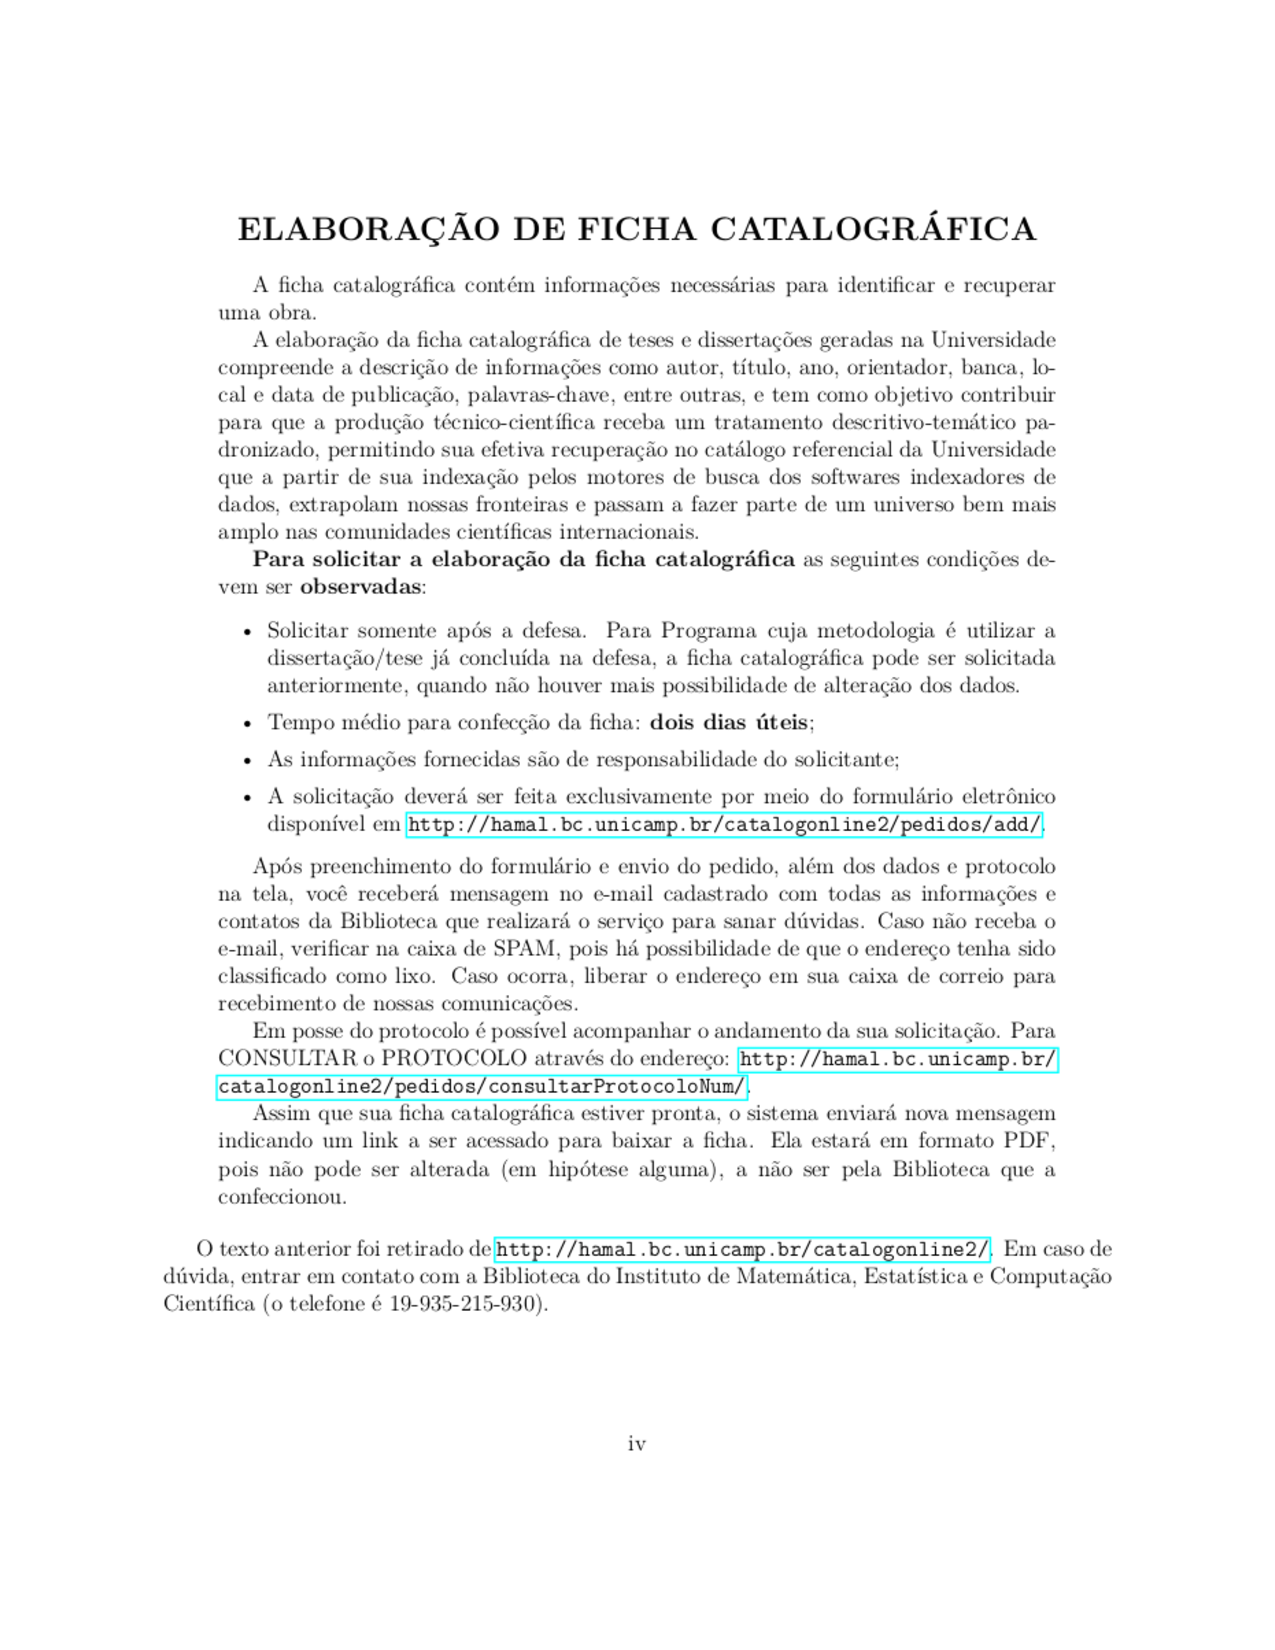
\includepdf[pagecommand={\thispagestyle{empty}}]{ficha-catalografica}
%\clearpage

%%% FOLHA DE APROVAÇÃO (Se for descomentar, a trava já está aplicada no pagecommand)
%\thispagestyle{empty}
%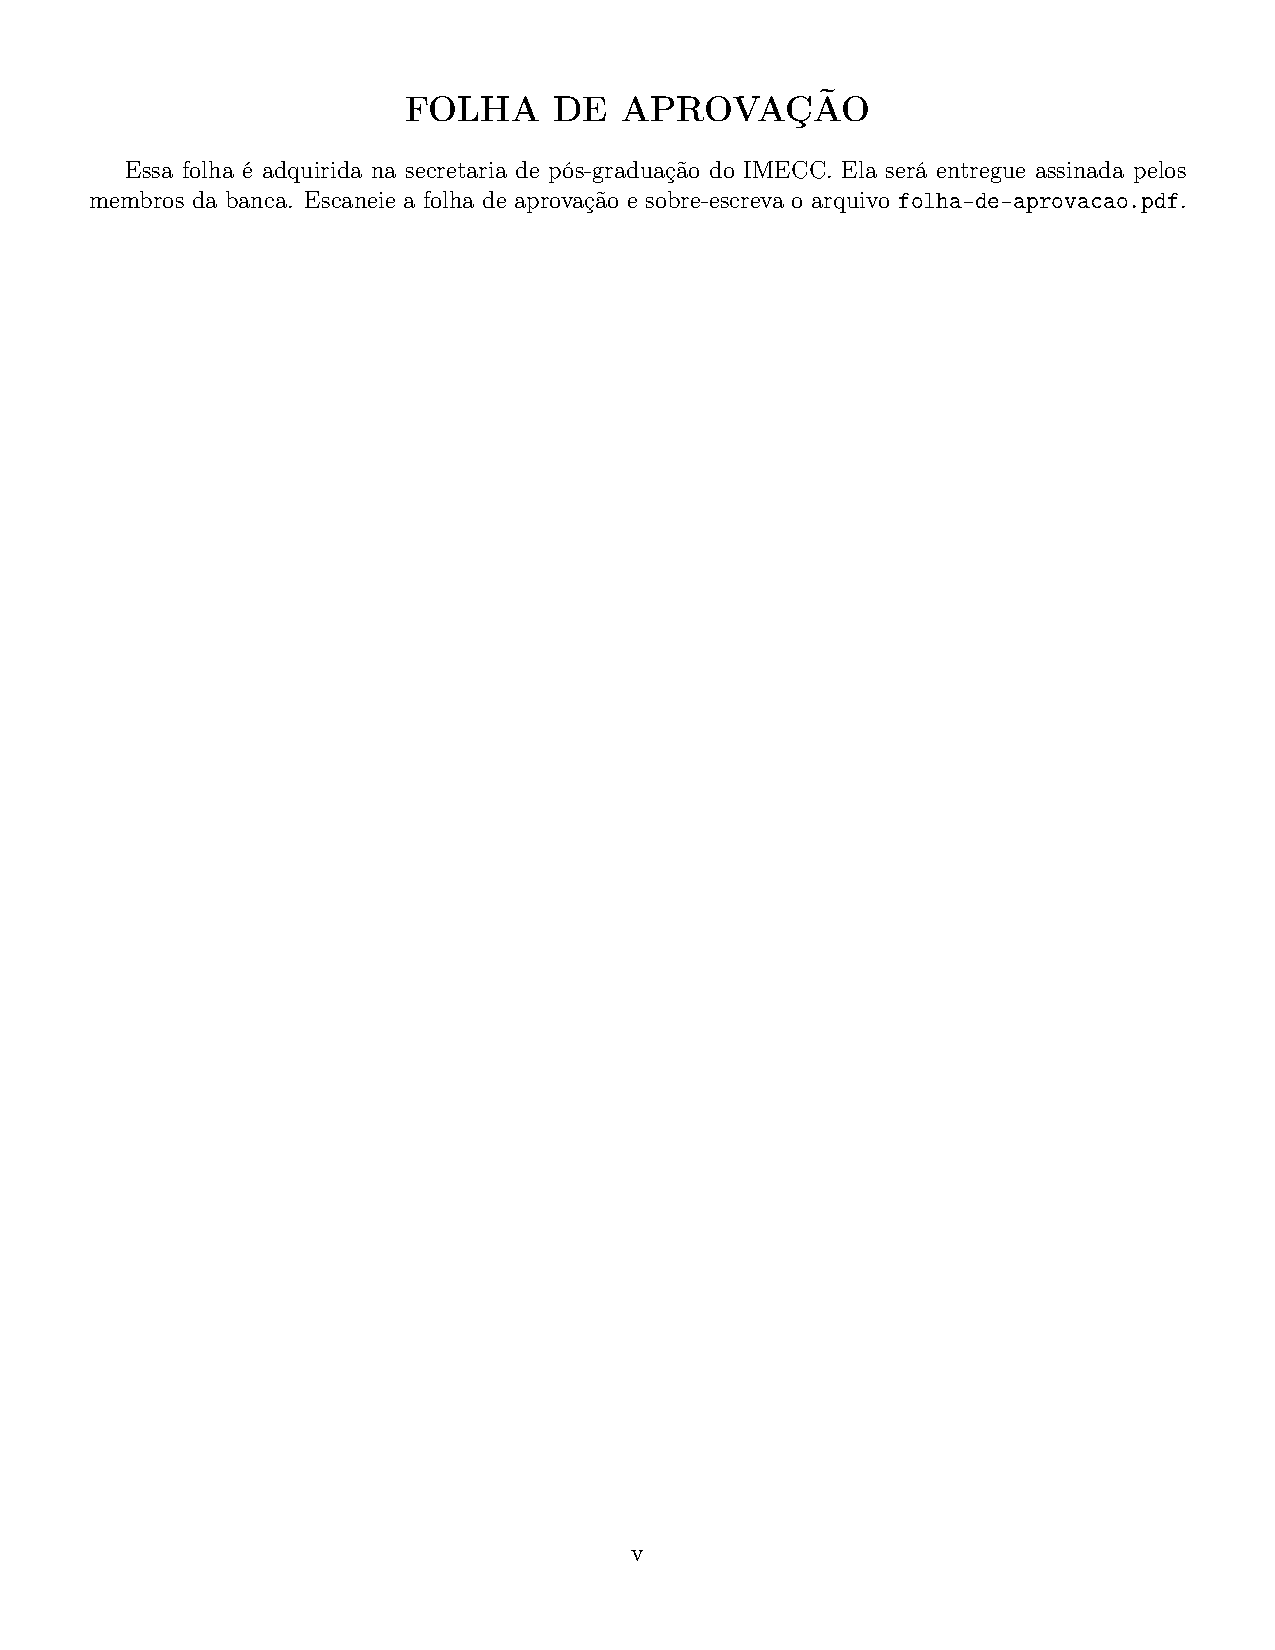
\includepdf[pagecommand={\thispagestyle{empty}}]{folha-de-aprovacao}
%\clearpage

%%% DEDICATÓRIA
\thispagestyle{empty}
\chapter*{\markboth{}{}}  % \markboth{}{} é utilizado para corrigir o cabeçalho.
\phantomsection
\addcontentsline{toc}{chapter}{Dedicatória}
\begin{center}
  \emph{
  % FIXME Remover as duas linhas abaixo.
  Aos meus \ldots. \\
  Para \ldots.} 
\end{center}

\begin{figure}[!htb]
  \center
  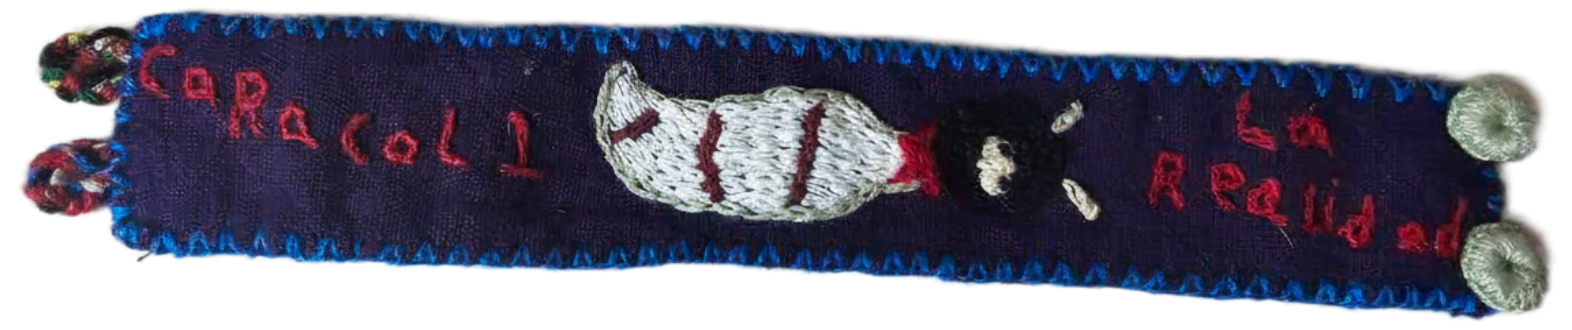
\includegraphics[width=0.8\textwidth]{figuras/caracol_colorido.png}
  \caption*{\textit{Lento, pero avanzo}. Caracol 1, Chiapas, México, dezembro de 2022.}
  \label{fig:scielo_temporal}
\end{figure}

%\begin{figure}[!htb]
 % \center
  %\includegraphics[width=0.8\textwidth]%{figuras/caracol1.png}
  %\caption*{\textit{Lento, pero avanzo}. Caracol 1, %Chiapas, México, dezembro de 2022.}
 % \label{fig:scielo_temporal}
%\end{figure}

%[INSERIR POEMA DE AUTORIA PRÓPRIA SOBRE A VIAGEM AO MÉXICO]


\thispagestyle{empty}
\clearpage

%%% AGRADECIMENTOS
\thispagestyle{empty}
\chapter*{Agradecimentos\markboth{Agradecimentos}{}}  % \markboth{}{} é utilizado para corrigir o cabeçalho.
\phantomsection
\addcontentsline{toc}{chapter}{}
% FIXME Escrever os agradecimentos.
%Sempre que me sinto perdida de meus valores, lembro-me dos meus amigos ... 
%Se recebeu bolsa de algum órgão de fomento, não esqueça de agradecê-lo.

O presente trabalho foi realizado com apoio da Coordenação de Aperfeiçoamento de Pessoal de Nível Superior --- Brasil (CAPES) --- Código de Financiamento 001.
\thispagestyle{empty}
\clearpage

%%% EPÍGRAFE
\thispagestyle{empty}
\chapter*{\markboth{}{}}  % \markboth{}{} é utilizado para corrigir o cabeçalho.
\phantomsection
\addcontentsline{toc}{chapter}{Epígrafe}
\vfill
\begin{flushright}
  \textit{Caminante, son tus huellas\\
  el camino y nada más;\\
  Caminante, no hay camino,\\
  se hace camino al andar.\\
  Al andar se hace el camino,\\
  y al volver la vista atrás\\
  se ve la senda que nunca\\
  se ha de volver a pisar.\\
  Caminante no hay camino\\
  sino estelas en la mar.}
  
  \vspace{0.5cm}
  
  --- Antonio Machado, \enquote{Proverbios y cantares}, XXIX, \textit{Campos de Castilla}
\end{flushright}
\vfill
\thispagestyle{empty}
\clearpage

%%% ==================== FIM DO BLOCO ISOLADO ====================

%%% RESUMO
\chapter*{}
\thispagestyle{empty}
\addcontentsline{toc}{chapter}{Resumo}
% ============================================================
% RESUMO — versão original de Juliane com acréscimos mínimos
% Mudanças: (1) "conduziu" -> "me levou" (regra 14); (2) frase curta
% sobre as duas linhas do capítulo 2; (3) enxertos "não só sobre, mas
% com" e auditabilidade na frase das inscrições; (4) "o conceito de
% tecnografias que proponho", direto, sem trajetória; (5) palavra-chave.
% ============================================================
\begin{center}
  \large{\textbf{Resumo}}
\end{center}
\selectlanguage{brazilian}
\begingroup
\setstretch{1.2}
\noindent O que cientistas e engenheiros fazem quando desenvolvem inteligência artificial? Movida por essa questão, segui pesquisadores ao longo de quatro anos de trabalho etnográfico no Centro de Inteligência Artificial da Universidade de São Paulo, um dos Centros de Pesquisa Aplicada da Fundação de Amparo à Pesquisa do Estado de São Paulo. O centro foi criado em 2020 mediante convênio entre a fundação, a universidade e a International Business Machines Corporation. Quando iniciei a pesquisa em 2022, a parceria parecia estável; quando a finalizei em 2025, a corporação havia encerrado o convênio. O período estendido de campo permitiu descrever o arranjo das práticas tecnocientíficas da rede sociotécnica que associou universidade pública e corporação transnacional na pesquisa de inteligência artificial no Brasil, da fundação à dissolução. Ao seguir Fábio e Cláudio, diretores do Centro, a pesquisa atravessou a história da relação entre o centro e a corporação e as práticas tecnocientíficas corporativas ao longo do tempo. Ao seguir Marcelo Finger, coordenador do projeto Sistema de Detecção Precoce de Insuficiência Respiratória baseada em Análise de Áudio, a pesquisa seguiu a cadeia de translações que converteu gravações de fala de pessoas hospitalizadas com Covid-19 em espectrogramas (representações visuais do som) processados por redes neurais para detecção de insuficiência respiratória através da análise da voz. Esse movimento etnográfico de seguir os atores por onde quer que fossem levou a tese por vários sítios, e foi esse movimento que me levou à escolha da teoria ator-rede como orientação teórico-metodológica capaz de dar conta do campo. No percurso, uma análise lexicométrica de seis obras de Bruno Latour e um mapeamento bibliométrico dos estudos sobre inteligência artificial nas ciências humanas brasileiras compõem a revisão de literatura da tese. Ao longo da pesquisa, feita não só \textit{sobre}, mas \textit{com} a inteligência artificial generativa, a produção de conhecimento etnográfico mobilizou um conjunto de práticas de inscrição tecnocientífica: diagramas interativos em Mermaid, análises em Python, modelos de linguagem (Claude, Anthropic), espectrogramas, construção de site para apresentação da defesa, com auditabilidade pública das técnicas em repositórios do GitHub. Essas grafias tecnocientíficas constituem o conceito de tecnografias que proponho, designando o modo de pesquisa que habita a tensão entre a circulabilidade técnica das inscrições e a realidade sensível dos corpos humanos. A pesquisa contribui para os estudos de ciência e tecnologia ao demonstrar que seguir múltiplos atores em um centro de pesquisa em inteligência artificial permite analisar tanto as negociações institucionais e corporativas que sustentam a pesquisa em inteligência artificial quanto as práticas tecnocientíficas situadas de desenvolvimento de sistemas, investigando como esses dois planos se articulam na produção de conhecimento em inteligência artificial e na produção de conhecimento sobre inteligência artificial pelas ciências sociais.

\noindent \textbf{Palavras-chave}: Inteligência Artificial; Tecnografias; Teoria Ator-Rede; Práticas Tecnocientíficas; Estudos de Ciência e Tecnologia.
\endgroup
\selectlanguage{brazilian}
\clearpage

%%% ABSTRACT
\chapter*{}
\thispagestyle{empty}
\addcontentsline{toc}{chapter}{Abstract}
\begin{center}
  \large{\textbf{Abstract}}
\end{center}
\selectlanguage{english}
\begingroup
\setstretch{1.2}
\noindent What do scientists and engineers do when they develop artificial intelligence? Driven by this question, I accompanied researchers over four years of ethnographic work at the Artificial Intelligence Center of the University of São Paulo, one of the Applied Research Centers of the São Paulo Research Foundation. The center was created in 2020 through an agreement between the foundation, the university, and the International Business Machines Corporation. When I began the research, in 2022, the partnership appeared stable; when I finished it, in 2025, the corporation had ended the agreement. The extended fieldwork period made it possible to describe the arrangement of technoscientific practices within the sociotechnical network that linked the public university and the transnational corporation in artificial intelligence research in Brazil, from its foundation to its dissolution. By following Fábio Cozman and Cláudio Pinhanez, the center's directors, the research traversed the history of the relationship between the center and the corporation and the corporation's technoscientific practices over time. By following Marcelo Finger, coordinator of the project Early Detection System for Respiratory Failure based on Audio Analysis, I traced the chain of translations that converted speech recordings of patients hospitalized with Covid-19 into visual representations of sound, processed by neural networks for the detection of respiratory failure through voice analysis. This ethnographic gesture of accompanying actors wherever they went led the thesis through multiple sites, and it was this movement that led me to choose actor-network theory as the theoretical and methodological orientation capable of accounting for the field. Along the way, a lexicometric analysis of works by Bruno Latour situated the conceptual vocabulary I mobilize, and a bibliometric mapping of studies on artificial intelligence in the Brazilian humanities situated this thesis within the field in which it intervenes. Throughout the research, carried out not only \textit{about} but \textit{with} generative artificial intelligence, the production of ethnographic knowledge mobilized a set of technoscientific inscription practices: interactive diagrams, computational analyses, artificial intelligence, charts, graphs, programming languages, and the construction of a website for an interactive reading of the thesis. These technoscientific inscriptions constitute the concept of technographies that I propose, and they designate a mode of research that inhabits the tension between the technique of inscriptions and the sensible reality of human bodies. By following actors in an artificial intelligence research center, this thesis contributes to science and technology studies by describing, within a single trajectory, the institutional and corporate negotiations that sustain artificial intelligence research and the situated technoscientific practices of system development, and by showing how these two planes articulate.

\noindent \textbf{Keywords}: Artificial Intelligence; Ethnography; Technographies; Technoscientific Practices; Science and Technology Studies.
\endgroup
\selectlanguage{brazilian}
\clearpage

%%% LISTA DE ILUSTRAÇÕES
\renewcommand{\listfigurename}{Lista de Ilustrações}
\listoffigures
\thispagestyle{empty}
\clearpage

%%% LISTA DE TABELAS
\listoftables
\thispagestyle{empty}
\clearpage

%%% ABREVIAÇÕES
\input{abreviacoes}
\clearpage

%%% SÍMBOLOS
\input{simbolos}
\clearpage

%%% SUMÁRIO
\tableofcontents
\thispagestyle{empty}
\clearpage

%%%%%%%%%%%%%%%%%%%%%%%%%% CORPO %%%%%%%%%%%%%%%%%%%%%%%%%%
\clearpage
\assignpagestyle{\chapter}{plain} % Devolve o comportamento normal para os capítulos textuais
\pagenumbering{arabic}
\hypersetup{pageanchor=true} 
\pagestyle{fancy}

% ex_cap0.tex
\chapter*{Apresentação}
\addcontentsline{toc}{chapter}{Apresentação}
\markboth{Apresentação}{Apresentação}   % cabeçalho, se usar pagestyle com cabeçalho

Em março de 2022 estava no InovaUSP, em São Paulo, para minha primeira visita ao Centro de Inteligência Artificial da Universidade de São Paulo (C4AI). Descobri o lugar por acaso. A inteligência artificial (IA) não fazia parte de meu projeto inicial de pesquisa de doutorado, mas um amigo, sabendo de meus novos interesses acadêmicos pelos estudos de ciência e tecnologia, enviou-me via WhatsApp uma notícia sobre a inauguração de um centro de pesquisas em IA instalado na USP. A mesma curiosidade que me levou a abrir aquele link motivou-me a escrever para João, coordenador do Observatório da Inteligência Artificial e Impacto Social (OBIA) do C4AI. Expliquei minhas intenções de pesquisa, mencionando as disciplinas sobre ciência e tecnologia que havia cursado e um texto de Kate Crawford e Vladan Joler sobre a Amazon Echo\footnote{O texto 
em questão, \emph{Anatomia de um sistema de inteligência artificial} \parencite{Crawford2018Anatomy}, foi um dos primeiros que li sobre  inteligência artificial e, de certa forma, inspirou-me a começar esta pesquisa. 
A versão original do mapa, em inglês, está disponível em: 
\url{https://anatomyof.ai}. A tradução brasileira, por Cristiana Gonzales 
e Pedro P. Ferreira, foi publicada pela revista \textit{ComCiência} 
(Unicamp/Labjor) em 20 de setembro de 2020 e está disponível em: 
\url{https://www.comciencia.br/anatomia-de-um-sistema-de-inteligencia-artificial/}. 
Acesso em: 6 abr. 2026.}

João me guiou pelas instalações físicas do Centro. Ao me aproximar da sala principal de convivência dos pesquisadores, notei que a porta estava fechada, mas uma parede inteira de vidro expunha todo o interior ao corredor. Parei ali por alguns instantes, observando através do vidro. Fileiras de computadores ocupavam estações de trabalho compartilhadas. Naquele dia, não havia ninguém na sala; ainda assim, a transparência seletiva daquele espaço me intrigou. Era possível imaginar os pesquisadores, acompanhar o trabalho que ali aconteceria, mas a porta fechada indicava que a entrada era controlada. Era um espaço parcialmente aberto: a parede de vidro permitia ver o interior, mas a porta controlava quem entrava. Será que era ali o ``laboratório do C4AI''? Pensava com a expectativa de encontrar tal lugar.

Enquanto caminhávamos pelos corredores, algo chamou minha atenção. Uma sala trancada que, através de uma pequena janela de vidro na porta de madeira, permitia vislumbrar um pouco do que havia em seu interior. Pareciam ser vários gabinetes de computadores que, mais tarde, eu descobriria tratar-se das unidades de processamento, as chamadas GPUs (\textit{Graphics Processing Units)} utilizadas para processar dados em alta velocidade e em paralelo, interligadas por uma extensa rede de cabeamento estruturado. No início desta pesquisa, em 2022, não era comum que imagens do interior de \textit{data centers} circulassem publicamente, e a quantidade de máquinas concentradas naquela sala era, para mim, algo inédito, uma materialidade da computação que o uso cotidiano de computadores pessoais e sistemas de inteligência artificial raramente traz à tona.\footnote{Ursula K. Le Guin, em ensaio de 2005, criticava o uso da palavra \enquote{tecnologia} como sinônimo exclusivo de alta tecnologia: \textit{Technology is the active human interface with the material world}. Texto disponível em: \url{https://www.ursulakleguin.com/a-rant-about-technology}, acesso em: 21 jan. 2026. A IA começa na extração mineral, na fabricação de cristais de silício, na circulação da eletricidade através de transistores, e essa cadeia de mediações não aparece no uso cotidiano dos sistemas. Como Lécuyer e Brock demonstram, as histórias convencionais da microeletrônica são \textit{under materialized}: focam excessivamente no design de dispositivos e deixam de lado as redes centradas na produção e manipulação de materiais semicondutores \parencite{LecuyerBrock2006Materiality}. Em certo sentido, ensinou-se pedras a fazer cálculos, e cálculos a escrever e a criar imagens.} Perguntei se aquela sala era o laboratório do Centro. Afinal, ali estavam as máquinas potentes que eu esperava encontrar. Mas não havia cientistas trabalhando, nem qualquer atividade humana visível; as GPUs estavam ali, estáticas, sozinhas, e o único movimento era o piscar rítmico de suas luzes. João disse que não, explicou que era como se fosse a área de TI (Tecnologia da Informação) do Centro. Respondi com um ``Ah!'' monossilábico, com certo constrangimento, e seguimos caminhando.

A situação, no entanto, acabou se transformando em um \textit{problema} de pesquisa\footnote{A noção remete ao convite de Donna Haraway, em \textit{Staying with the Trouble}, para \enquote{ficar com o problema}. Não encontrar o laboratório e os cientistas não é um problema a ser resolvido. É um problema que a pesquisa tensiona ao longo do tempo sem a pretensão de oferecer uma resolução ou uma resposta permanente \parencite{Haraway2016Staying}.}: \textit{onde está o laboratório de IA e onde estão os seus cientistas?} Eu tinha a expectativa de encontrar um lugar cheio de supercomputadores e cientistas desenvolvendo pesquisa em inteligência artificial. Mas eles não estavam lá, nem estiveram pelos anos seguintes de realização desta pesquisa. Havia uma sala com infraestrutura de microprocessadores para treinar modelos de IA e outra com computadores de mesa para uso dos pesquisadores, onde às vezes eu encontrava alguns deles, mas nunca ficavam por muito tempo. A pandemia de Covid-19 havia acabado de recuar, mas o padrão se manteria ao longo dos quase quatro anos que se seguiram, o laboratório continuaria existindo de forma não centralizada e os pesquisadores trabalham remotamente, compartilhando infraestruturas computacionais acessadas à distância.\footnote{Durante a entrevista com Fábio, diretor do Centro, ele também comentou esse aspecto distribuído quando mencionei que raramente via pesquisadores reunidos no espaço. Fábio observou: \enquote{A gente começou o centro na pandemia e depois as pessoas passaram a vir menos no local de trabalho [...] Eu sinto falta de um pouco de mais conexão [...] Antes da pandemia era mais forte. [...] quando o C4AI começou, eu tinha muita dúvida de como a gente ia conseguir fazer um centro tão disperso, tanta gente em tanto lugar. Isso não foi dificuldade nenhuma.} Essa reflexão orienta a discussão sobre o laboratório distribuído desenvolvida nos capítulos seguintes desta tese.}

Oito meses depois, em 30 de novembro de 2022, a OpenAI lançou o ChatGPT, disponibilizado gratuitamente como \enquote{pesquisa prévia}. O \textit{chat} ganhou popularidade rapidamente e atingiu mais de 1 milhão de usuários em cinco dias. A inteligência artificial deixava de ser objeto de pesquisa de círculos acadêmicos especializados e se tornava fenômeno de massa, presente nos debates públicos e nas manchetes de jornal. Enquanto isso, o laboratório que eu visitara em março continuava operando silenciosamente: os cientistas seguiam trabalhando remotamente, as GPUs processavam modelos, as mesas permaneciam vazias. A explosão pública da IA generativa não alterou a rotina de pesquisa do C4AI; intensificou, porém, o estranhamento da minha pergunta inicial. Se a IA parecia estar em quase todo lugar, nos \textit{smartphones} e nas conversas de não-especialistas, onde exatamente estava o laboratório que a produzia? Para entender isso, como descobriria, teria que investigar o que \enquote{laboratório} e \enquote{fazer tecnociência} querem dizer nesse contexto. 

Para investigar o que é um laboratório de IA e como os pesquisadores do C4AI fazem IA, \textit{segui} cientistas e engenheiros em ação \parencite{Latour1987Science}.\footnote{O subtítulo desta tese, \textit{como seguir cientistas e engenheiros --- universidade afora}, é uma variação do subtítulo de \textit{Ciência em Ação}, \textit{como seguir cientistas e engenheiros sociedade afora}. Nesse deslocamento, \enquote{sociedade afora} dá lugar a \enquote{universidade afora}, e o travessão marca a passagem do dentro para o fora do Centro. Dessa maneira, retomo a primeira regra de método de Latour, que consiste em \textit{seguir} cientistas e engenheiros nos momentos e locais em que produzem fatos e máquinas (tecnociência). Faço isso, contudo, a partir de um centro de pesquisa universitário cuja atuação se estende para além da USP, seja na relação com corporações transnacionais e agências de fomento (capítulo~\ref{capitulo3}), seja na articulação com hospitais durante a pandemia de Covid-19 (capítulo~\ref{capitulo4}).} Na prática, isso implicou (efetivamente) \enquote{seguir}\footnote{A palavra \enquote{seguir} assume um sentido particular nesta tese, pois remete ao ato de ir atrás ou observar algo ou alguém, em geral à distância. Isso difere de modo significativo de \enquote{acompanhar}, termo mais recorrente em contextos etnográficos. Acompanhar sugere que a presença do etnógrafo é desejada ou valorizada; algo distinto de apenas autorizar ou consentir com essa presença. Esse ponto é central para esta etnografia, pois delimita o que é ou não é possível observar, descrever e/ou analisar. Assim, \enquote{seguir} aqui se configura como um posicionamento ético-onto-epistemológico no sentido que \textcite{Barad2007Meeting} dá ao termo, conforme desenvolvido no Capítulo~\ref{capitulo1}.} cientistas e engenheiros como Fábio e Cláudio, diretor e vice-diretor do C4AI, em eventos de divulgação e difusão científicas realizados dentro e fora da universidade, tanto presencialmente quanto de forma remota. Seguir esses atores, que acabam se tornando centrais nesta tese, levou-me ao que os pesquisadores do C4AI chamavam de \enquote{parceria} e a Fapesp chamava de \enquote{convênio},\footnote{Ao longo desta tese, \enquote{parceria} e \enquote{convênio} são categorias nativas, não analíticas. \enquote{Parceria} circulava entre os pesquisadores do C4AI para descrever a relação com a IBM. \enquote{Convênio} era o termo institucional da Fapesp. As duas palavras coexistiram no campo.} ou como prefiro chamar, a \enquote{relação} entre uma universidade pública (USP), uma fundação de apoio à pesquisa (Fapesp) e uma empresa multinacional (IBM).\footnote{O debate sobre parcerias público-privadas é um tema controverso. Glauco Arbix, por exemplo, coordenador da Cátedra de IA Responsável USP-Google (lançada em dezembro de 2025), argumenta que a autonomia universitária pode ser preservada nessas colaborações e que a soberania tecnológica se constrói \enquote{capacitando pessoas} em contato com \enquote{quem está na fronteira}, não isolando universidades. Entrevista ao podcast UAI, fevereiro de 2026. Disponível em: \url{https://www.youtube.com/watch?v=8aoglGSC1ys}. Acesso em: 28 fev. 2026.} Meu trabalho de campo começou em março de 2022; o período anterior, da fundação do Centro em outubro de 2020 até a minha entrada, eu o reconstituí pelos relatórios institucionais e pelas entrevistas, e é como reconstrução, e não como observação direta, que ele entra nesta tese. É com essa ressalva que conto aqui a história dessa relação, da fundação em outubro de 2020 à dissolução da parceria em dezembro de 2025. A parceria C4AI-IBM chegou ao fim enquanto eu concluía a escrita desta tese, o que tornou necessário revisar grande parte dos argumentos que haviam sido desenvolvidos até então.

Chamo esta tese de uma tecno-etnografia, e a grafia importa. Escrevo-a em \texttt{LaTeX}, ambiente de composição de texto que aprendi a usar no próprio campo, ao ver os pesquisadores do \texttt{C4AI} trabalharem com ele e ao adotá-lo por achá-lo melhor de trabalhar do que os editores que eu usava antes. Em certo momento da pesquisa me perguntei quais marcas o campo estava deixando em mim, e aprender a escrever em \texttt{LaTeX} foi uma delas, no registro do ser afetado que retomo no capítulo~\ref{capitulo1}. A notação com que inscrevo esta tese é, então, ela mesma um vestígio do que observei, e do que o campo fez comigo enquanto eu o observava. No \texttt{LaTeX}, as chaves \texttt{\{\ \}} delimitam um bloco, um corpo que pertence junto como unidade, ao passo que os colchetes \texttt{[\ ]} delimitam o que é opcional, acrescentado de fora. Na sintaxe das citações que uso em todo o texto, \texttt{\textbackslash parencite[p.~19]\{strathern1995relation\}}, o que está em chaves é a obra, o corpo constitutivo da referência, e o que está em colchetes é a página, o acréscimo aplicado de fora. Penso a tecno-etnografia, então, como aquilo que entra em \texttt{\{\ \}}, pois técnica, tecnologia e etnografia formam um só escopo, um bloco que se constitui como unidade, em lugar de \texttt{[\ ]}, que inscreveria uma técnica acrescentada de fora a uma etnografia que lhe preexistisse. Um método aplicado aos objetos seria o colchete, \texttt{[método]\{objeto\}}, ao passo que o conceito da prática que proponho é a chave, \texttt{\{tecno-etnografia\}}. Com isso quero dizer que a tecno-etnografia não é um método que eu trouxesse pronto para aplicar ao \texttt{C4AI}, e sim um conceito que se constitui no próprio gesto de pôr em relação o campo, a teoria, as minhas memórias de pesquisa e os modelos de linguagem com que escrevo. Esse gesto se desdobra ao longo dos quatro capítulos, e no capítulo~\ref{capitulo2} retomo o seu sentido teórico, em diálogo com a noção de relação de \textcite{strathern1995relation}, ponto em que nomeio o próprio gesto de pôr em relação como o que constitui a tecno-etnografia enquanto conceito da prática.\footnote{Volto a esse trocadilho e ao conceito de relação de Strathern no capítulo~\ref{capitulo2}, ao discutir a sociologia do conhecimento de Harry Collins e o que muda na pergunta sobre o que pode ser transferido a uma máquina quando se passa dos sistemas especialistas aos modelos de inteligência artificial generativa.}

%figuração como modo de pensamento 

% [NOTA DE REVISÃO 1] Parágrafo realinhado à formulação revisada no capítulo 3: a figuração têxtil e o diagrama põem ambos em relação, cada um em um plano próprio (tempo/espessura vs. superfície/simultaneidade). Removida a negação de relacionalidade ao diagrama ("não mostram o relacionar") e a fórmula "não é X, e sim Y" (R4). A resistência da têxtil à superfície e a pergunta final se mantêm.
Esse gesto de pôr em relação tem uma consequência que percorre toda a tese. Penso esta tese por uma figuração têxtil, em que o trabalho de pesquisa se faz de fios, tramas, costuras, nós e cortes, e ao mesmo tempo inscrevo o seu percurso em diagramas e mapas que disponho ao longo dos capítulos para situar quem lê. As duas coisas põem em relação, e a diferença entre elas me interessa, pois cada uma relaciona em um plano próprio. A figuração têxtil é o modo como penso e construo o argumento, e trabalha no tempo e na espessura do pensamento que se tece, onde o ato de relacionar não vem dado de antemão e se refaz a cada vez. O diagrama põe em relação numa superfície plana, na simultaneidade do que se apreende de um só golpe de vista, e ao dispor nós e conexões faz aparecer ligações que a escrita sequencial não alcança.\footnote{Uso ao longo desta tese um conjunto de expressões que compõem um vocabulário --- \enquote{fazer aparecer}, \enquote{tornar visível}, \enquote{tornar legível}, \enquote{dar a ver}, \enquote{deixar ver}, \enquote{tornar inteligível} ou \enquote{compreensível} e correlatas --- cuja força semântica pode sugerir que as coisas se mostrem por si, ou que um acontecimento ou uma inscrição as revele. Não é o que afirmo. As coisas estão lá; o que muda é para onde olho e como olho. A visibilidade não é propriedade do objeto nem efeito de um acontecimento: é resultado do meu gesto de dispor, olhar, interpretar e analisar, a partir da posição situada de onde sigo a rede. Quem torna visível ou legível sou eu, e não o objeto que descrevo, a figura que componho ou o desfazer-se de um arranjo. Conservo essas expressões pela sua economia, com a ressalva de que, onde aparecem, é sempre o meu gesto de análise que está em jogo, e não uma autorrevelação do campo.} Reconheço, porém, que a figuração têxtil resiste a essa superfície, e que não consigo desenhá-la como desenho um mapa, porque o que ela figura é o próprio ato de relacionar em seu fazer-se, com o tempo e a espessura que a superfície achata. Habito, então, uma tensão, pois pratico na escrita um modo de relacionar que excede a superfície em que inscrevo os mapas, e os dois coexistem sem que um se reduza ao outro. Daí a pergunta que carrego pela tese inteira: se a figuração têxtil é um modo de pensar, e se o que reúne as coisas é uma relação que nunca está dada, como se pensa por tramas, como se mostra esse pensar, e o que acontece quando ponho em questão a própria diferença entre tecer um argumento e mapeá-lo.

O capítulo~\ref{capitulo1} descreve a minha entrada em campo e, a partir dela, define o conceito de tecno-etnografia que dá nome a este trabalho. Parto da pergunta sobre onde está o laboratório dos pesquisadores de IA do C4AI e dos seus cientistas, e a desdobro em três gestos analíticos: o corte que delimita uma rede que de outro modo se daria a ver como infinita, em diálogo com Strathern, Barad, Haraway, Costa e Law; a descrição das existências parciais que se compõem comigo e com a inteligência artificial generativa no trabalho de análise desta tese, das quase-máquinas e da agência distribuída à multiplicidade ontológica e ao fazer-com modelos de linguagem; e a compostagem que põe a fermentar materiais que o desenho da pesquisa mantinha separados. Esse trabalho ganha maior aprofundamento nos capítulos~\ref{capitulo3} e \ref{capitulo4}, onde investigo com mais detalhes como cientistas e engenheiros fazem IA a partir das redes sociotécnicas que construíram e de um sistema de IA em particular feito para detectar insuficiência respiratória (o Spira).\footnote{A análise da relação C4AI-IBM gerou também uma publicação que deriva desta tese: \textit{The C4AI Case: Governance and Accountability in a Brazilian Public-Private AI Partnership}, apresentada na conferência DASGRI 2026 (\textit{Track 3: Algorithmic Fairness, Transparency, and AI Ethics}), aceita para publicação pela Springer.} O capítulo~\ref{capitulo2} faz uma revisão da literatura em duas linhas de trabalho que percorri lado a lado. A primeira é uma análise lexicométrica de seis obras de Bruno Latour (e de Latour e Woolgar em \emph{Laboratory Life}), em que meço o quanto ele descreve a tecnociência em vocabulário militar e mostro que ele revê alguns dos seus termos sem rever esse vocabulário, ao lado das figurações de Haraway e Stengers que propõem outros modos de lidar com os aliados. Entre as duas linhas, percorro as leituras que cada problema do campo convocou: os estudos sociais da ciência e da tecnologia, a antropologia de Diana Forsythe e a sociologia dos sistemas especialistas de Harry Collins como primeiros estudos sobre inteligência artificial nas ciências sociais, uma discussão sobre mediação técnica e agência distribuída em sistemas de IA generativa, e as genealogias críticas do poder técnico. A segunda linha é um mapeamento bibliométrico do estado emergente das pesquisas sobre inteligência artificial nas ciências humanas brasileiras, feito sobre três bases, o Catálogo de Teses e Dissertações da CAPES, a coleção brasileira da SciELO e a base internacional OpenAlex. O capítulo~\ref{capitulo3} descreve a rede sociotécnica que Fábio e Cláudio construíram ao longo da relação C4AI-IBM, e produz cinco observações analíticas: a IBM contribuía com menos recursos do que USP e Fapesp, mas participava das conversas sobre direções de pesquisa; grupos que nasceram dentro do C4AI foram ganhando vida própria e tornaram-se centros independentes; temas de pesquisa mudaram de direção ao longo de 2020--2025, às vezes por iniciativa dos pesquisadores, às vezes após interlocuções com a IBM; enquanto a relação encerrava no Brasil, a IBM expandia relações em outros países como a Índia; e quando tudo acabou, parecia que a IBM nunca tinha estado ali. Isso me surpreendeu. Enquanto eu seguia Fábio e Cláudio, a IBM parecia o centro de gravitação do C4AI, o ponto a partir do qual tudo se organizava e fazia sentido. Por isso, o capítulo também descreve o que o encerramento da relação deu a ver sobre o quanto a continuidade do \texttt{C4AI} dependia da \texttt{IBM} como financiador, o que enquanto a relação durava não se distinguia na rotina do Centro. Já o capítulo~\ref{capitulo4} investiga como práticas tecnocientíficas situadas na construção de sistemas de IA são feitos dentro desses arranjos sociotécnicos.

Esses quatro capítulos estão organizados em uma ordem que importa para o argumento desta tese. Os dois primeiros (capítulos~\ref{capitulo1} e~\ref{capitulo2}) fazem trabalho reflexivo sobre o vocabulário com que se descreve a tecnociência; os dois últimos (capítulos~\ref{capitulo3} e~\ref{capitulo4}) descrevem etnograficamente o \texttt{C4AI} e o \texttt{Spira}. A ordem não é preparatória, em que o leitor passaria pelos dois primeiros para chegar aos dois últimos. É proposta argumentativa, isto é, faço o trabalho reflexivo antes da descrição etnográfica porque a tecnociência vem sendo descrita há quatro décadas em vocabulário militar-industrial (alistar, recrutar aliados, provas de força, vencer controvérsias), e descrever o \texttt{C4AI} e o \texttt{Spira} nesse vocabulário herdado significa naturalizar uma figuração específica da tecnociência, em que ela é combate, e fechar de antemão a possibilidade de descrevê-la de outros modos. Os capítulos~\ref{capitulo1} e~\ref{capitulo2} tornam visível em que vocabulário a tecnociência tem sido descrita e propõem outros vocabulários para descrevê-la, em diálogo com Donna Haraway, Marilyn Strathern, Isabelle Stengers, Suely Kofes e outras autoras. Ler os dois primeiros capítulos é, nesse sentido, parte do que esta tese faz como proposta, em lugar de fundo teórico que precede a etnografia propriamente dita.

Os capítulos foram sendo escritos e ganhando forma em momentos distintos, respondendo tanto ao desenvolvimento desta etnografia quanto às exigências acadêmicas próprias do doutorado. Tudo isso atravessa a composição da tese e se expressa no que cada capítulo se propõe a fazer. O capítulo 1 surgiu de uma preocupação em explicar como e por que cheguei ao tema da IA e ao C4AI, o que lhe conferiu um caráter mais descritivo e narrativo, com uma presença mais marcada da minha voz no texto. Soma-se a isso o contexto de lançamento público da IA generativa e o debate, acadêmico e não acadêmico, que se estruturou em torno dela, o que me colocou numa posição particular – eu diria mais vulnerável e responsável – em relação à IA. E, por estar realizando uma etnografia em um centro de IA, rapidamente a IA generativa se tornou quase uma obrigação de estudo, algo que eu necessariamente teria de abordar. Isso definitivamente não fazia parte do meu plano inicial. Foi, em grande medida, uma coincidência.

É curioso como essas coisas acontecem. À medida que eu me questionava sobre a IA generativa e era igualmente questionada sobre ela (boa parte da reflexão do capítulo 1 surge disso), fui sentindo a necessidade de aprofundar em seu estudo dentro do meu referencial analítico, inicialmente, e por curiosidade, a teoria ator-rede. Passei a me perguntar: o que podemos dizer sobre a IA generativa a partir da teoria ator-rede? E para além dela? Isso talvez soe como um desvio, um contorno (eu o chamaria de retorno à reflexão sobre a técnica e a tecnologia), em direção a um questionamento sobre como se faz IA para além do C4AI e o que ocorre quando quem também faz IA são pessoas como eu. Afinal, a IA, como eu viria a compreender, também é produzida por cada uma das pessoas não cientistas ou engenheiras que, de diferentes maneiras, fazem parte de seus sistemas: de forma direta, como fornecedoras da matéria-prima que alimenta esses sistemas (os dados), ou de forma indireta, enquanto usuárias, que também são responsáveis por um desenvolvimento colateral da IA via aprendizado por reforço (para além do fornecimento de dados). Isso, pelo menos, para começar.

A partir desse movimento, escrevi um capítulo ancorado tanto na minha experiência em campo com cientistas e engenheiros que produzem IA quanto na minha própria experiência com a IA generativa, experiência que, aliás, incorpora aquilo que entendo que ela seja e o que espero dela, e isso é fundamental. O que as pessoas acreditam que a IA generativa é, e o que esperam que ela faça, não apenas influencia (ou mesmo determina) o que a IA irá entregar ou o que será feito com ela, como também delimita o modo como avaliamos seus usos, suas habilidades, desempenho e responsabilidades, e  especialmente de quem opta por utilizá-la. % ============================================================
% [SUELY p. 23 do PDF de 12/05]: "nao simplifica? Não há a procura de conhecimento e atividade científica?"
O que as pessoas esperam dos sistemas de IA, isto é, que sejam previsíveis, justos, transparentes e seguros, não coincide totalmente com as condições que as corporações que os desenvolvem precisam sustentar para se manter no mercado, em que prazos de entrega, retorno sobre investimento e diferenciação competitiva pressionam decisões de pesquisa e desenvolvimento mesmo quando há atividade científica robusta envolvida. Além disso, a IA generativa é não determinística, o que é um sério desafio para a ciência da computação e para os fundamentos da automação. Porém, se a IA generativa não opera de modo contínuo, o que em grande parte das vezes produz imprevisibilidade e, consequentemente, erros e vieses, o que isso implica para sua aplicação nas ciências humanas e sociais? Enquanto este capítulo era escrito, vários órgãos reguladores e instituições de ensino superior formulavam suas próprias diretrizes e recomendações para o uso de IA generativa na educação universitária, e os pesquisadores começavam a divulgar estudos sobre suas aplicações e implicações para a sociedade e as ciências humanas e sociais. Foi movida por essa preocupação que dei forma ao capítulo 1 e, por isso, levei a sério o \enquote{aprender} com meus interlocutores, cientistas e engenheiros; eu precisava compreendê-los e, para isso, precisava aprender com eles. Esse caminho me conduziu ao capítulo 2. 

% [SUELY p. 23 do PDF de 12/05]: marcou três pontos neste parágrafo.
% (b) "espontâneo" duas vezes — Suely sinalizou: "esse tipo de deslocamento parecia ocorrer de forma bastante espontânea" e "pareceu-me também espontâneo realizar essa 'revisão bibliográfica'". A palavra apaga o gesto de decisão.
% (c) "outros mitovos" — typo. Suely marcou explicitamente.
O capítulo 2 tomou forma a partir de um duplo processo de aprendizagem: por um lado, junto aos colegas pesquisadores e professores do doutorado, nas disciplinas sobre ciência e tecnologia que frequentei; por outro, por meio dos cursos, encontros, observações, conversas e imersões realizados com cientistas e engenheiros da computação. Essa convivência com eles, em cursos de curta e longa duração, proporcionou-me uma compreensão bastante particular sobre suas formas de ver o mundo, suas ciências e as maneiras como enfrentavam os desafios e problemas próprios de sua área. Um desses cursos foi sobre ciência de dados e inteligência artificial, no qual aprendi os fundamentos da linguagem de programação Python voltada à análise de dados. Ao longo do curso, precisei desenvolver um projeto de análise de dados para aplicar os conceitos aprendidos. Naquele período, eu estava explorando as quase 500 publicações científicas do C4AI (que desenvolvo com mais detalhes no capítulo 3), e decidi utilizá-las como estudo de caso do curso, o que acabou também motivando uma investigação nas plataformas SciELO e CAPES sobre publicações relacionadas à IA produzidas nas ciências humanas e sociais. Diversificar as abordagens do referencial bibliográfico que sustenta esta tese tornou-se, então, parte do trabalho do capítulo. A análise bibliométrica derivou, portanto, de um processo de aprendizado com o campo e com os meus interlocutores, o que é diferente de uma escolha metodológica encaixada na pesquisa por outros motivos e demandas. Por isso, este capítulo tem natureza distinta do primeiro e dos demais: os modos de pensar mudaram conforme o campo se desdobrava, e cada capítulo carrega a marca da fase da pesquisa em que foi escrito. Eu mesma fui caminhando e me transformando junto com o meu campo e com as diferentes motivações e demandas que surgiam de todos os lados. E, como minha trajetória acadêmica envolve uma formação multidisciplinar em ciências sociais (tanto na graduação quanto na pós-graduação), esse tipo de deslocamento se compunha com a trajetória que eu vinha construindo. E, tendo em vista que minha principal inspiração vem da teoria ator-rede, pareceu-me coerente tratar essa \enquote{revisão bibliográfica} como parte do mesmo modo de produção de conhecimento das demais ciências, afinal, as ciências humanas e sociais compartilham o mesmo espaço de produção. Isso foi significativo demais para mim e para minha pesquisa para ser relegado a uma nota de rodapé ou a um apêndice desta tese, pois, assim como o capítulo 1, tratou-se de um \enquote{efeito etnográfico}, nos termos da antropóloga Marilyn Strathern, ou seja, a \textit{relação} entre o contexto de campo, a observação e o conhecimento teórico. Essa relação me proporcionou um novo modo de compreender como cientistas e engenheiros fazem IA, que foi \enquote{traduzido} de forma mais contundente nas \enquote{lições} do capítulo 1, mas que aparece em toda a tese, de uma forma ou outra.

% [SUELY p. 24 do PDF de 12/05]: duas observações neste parágrafo.
% (b) Sobre "de forma espontânea, passei a acompanhar cientistas e engenheiros": Suely sinalizou a palavra (mesma observação da p. 23).
Os capítulos 3 e 4 são aqueles mais etnográficos e concentram as contribuições mais originais e substantivas desta tese sobre como cientistas e engenheiros fazem IA e por que isso é importante, para quê e para quem. Ainda assim, esses capítulos, cada um à sua maneira (o capítulo 3 acompanha o \texttt{C4AI} seguindo um segmento longo de associações institucionais que se estende por mais de um século; o capítulo 4 acompanha o \texttt{Spira} seguindo um segmento curto e mais densamente atado, a cadeia de inscrição que vai da voz hospitalar ao espectrograma processado pela rede neural, sem que isso faça de uma rede maior ou menor que a outra), também fazem parte do mesmo \enquote{efeito etnográfico} dos capítulos 1 e 2. Como mencionei, também levei isso a sério e, em grande parte, como parte do desdobramento da pesquisa, passei a acompanhar cientistas e engenheiros. Foi assim que tomei conhecimento dos cursos e de outras oportunidades de aprendizado junto a eles. Porém, talvez a \enquote{perseguição} mais relevante tenha sido a de Fábio e Cláudio (diretor e vice-diretor do C4AI) e, justamente nesses momentos de consolidação do centro, acabei tendo uma visão privilegiada do início da relação C4AI-IBM-Fapesp ou, nos termos dos meus interlocutores, da parceria e/ou convênio estabelecido entre eles. Fábio era, antes de tudo, um cientista, enquanto Cláudio (que ainda trabalhava na IBM naquela época) se destacava principalmente como empreendedor, no sentido de detectar problemas e oportunidades tanto para a universidade quanto para o mercado, embora também fosse cientista. Pelo menos, era assim que eu os via. A ideia de construir redes veio dessa \enquote{perseguição} (e que intitula genericamente os capítulos 3 e 4, as redes que foram construídas por Fábio, Cláudio e Marcelo), pois, sem dúvida, era isso que eles estavam fazendo (e eu também, como perceberia um pouco mais adiante). Fazer rede é, principalmente e em acordo com a teoria  ator-rede, traduzir interesses heterogêneos em uma cadeia de associações que se sustente:\footnote{A imersão nas obras de Bruno Latour se fez também pelo seu \textit{site} pessoal (\url{http://www.bruno-latour.fr}), mantido pelo próprio autor até sua morte em 2022 e ainda ativo como acervo. Estruturado em seções de livros, artigos, conferências e cursos, o \textit{site} reúne materiais distintos, textos curtos publicados em revistas de arte, prefácios, conferências em vídeo, cursos ministrados e textos polêmicos circunstanciais. Acessar Latour por esse canal permitiu acompanhar sua produção canônica e o modo como ele próprio organizava o \textit{site} e a coerência entre seus textos. Uma operação de fazer rede com as suas próprias obras. O acesso a esses textos marginais e ainda em elaboração de Latour permitiu-me acompanhar de perto como se desenrolou o seu processo de trabalho, o qual vai se transformando à medida que ele os converte em artigos e, depois, em livros.} alinhar o que a USP quer, o que o C4AI quer, o que a IBM quer, o que a Fapesp quer, o que cada pesquisador quer, e fazer com que esses interesses, motivações e objetivos originalmente distintos, passem a se sustentar mutuamente. Quanto mais longa e mais articulada a rede, mais durável o que ela sustenta e, também mais frágil quando um de seus elos centrais se desfaz. As entrevistas que realizei com Fábio, Cláudio e Marcelo também desempenharam um papel fundamental na escrita dos capítulos 3 e 4 (pelos quais, aliás, sou profundamente grata), pois, além de trazerem contribuições empíricas relevantes para esta pesquisa, proporcionaram-me um aprendizado muito especial. Foi, em grande parte, esse processo de aprendizado que me deu fôlego e entusiasmo para escrever esta tese. Para Tim Ingold, em \textit{Antropologia: para que serve?} \parencite[pp.~16--17]{Ingold2019Antropologia}, o objetivo primordial da antropologia não é etnográfico, mas educativo: a observação participante é, antes de qualquer coisa, um compromisso de aprender com aqueles que tomamos como interlocutores, como faz o aprendiz com seu mestre, e a regra número um da disciplina é levá-los a sério. Subscrevo essa formulação, que no meu caso coincide com um traço pessoal na forma como me relaciono com as pessoas, com o mundo e com a vida. Aprender com Fábio, Cláudio e Marcelo gerou em mim um sentimento de compromisso com o tipo de pesquisa que eu vinha realizando e de responsabilidade com essas pessoas, pois, para além da denúncia, eu desejava \textit{fazer alianças sem ferir os sentimentos estabelecidos}, como propõe Isabelle Stengers e como é problematizado de maneira muito bonita por Clarissa Reche Nunes da Costa, colega de doutorado e de área de pesquisa. Mas tudo isso veio junto com tensões (permanentes) e conflitos (ainda sem solução), além de uma sensação persistente de que esta tese nunca vai realmente se concluir (ficará sempre incompleta). Isso porque o que iniciei aqui não é apenas uma tese de doutorado feita para cumprir formalmente uma etapa da pós-graduação, mas um tipo de compromisso e de responsabilidade que, enquanto existirem internet e arquivos digitais, continuará a reverberar por aí; e, além disso, é algo que vai me acompanhar pelo resto da vida, pois, mesmo que eu deixe de me interessar por ou estudar IA, esse percurso me abriu um novo mundo da tecnociência a conhecer e com o qual aprender. Não é impressionante? 

O capítulo 4 (``A rede que Marcelo construiu'') foi o momento em que esse novo mundo da tecnociência começou a se revelar para mim. Foi justamente nele que me deparei, pela primeira vez, com um sistema de IA: um sistema de detecção de insuficiência respiratória desenvolvido durante a pandemia de Covid-19 (o Spira). Esse encontro veio acompanhado tanto da história de sua criação (tal como relatada por Marcelo em entrevista) quanto da forma como esse processo foi descrito nos artigos científicos escritos por ele e por outros pesquisadores envolvidos no projeto. Eu nunca tive a intenção de concentrar a pesquisa na análise de um sistema específico de IA. Embora meu objetivo geral estivesse ligado a compreender como os cientistas fazem IA no C4AI, eu procurava por isso como quem busca agulhas em um palheiro, pois não sabia de antemão qual sistema apareceria em meu campo. Além disso, por conta de uma série de fatores relacionados à configuração distribuída e remota do centro (em parte devido à pandemia e em parte por outros motivos), alguns dos trabalhos dos pesquisadores do C4AI chegavam até mim de forma indireta, seja por acompanhá-los em eventos acadêmicos, seja pelas redes sociais do centro, como o LinkedIn. Em um primeiro momento, o que capturou minha atenção foi o conjunto de dados em português desenvolvido pelo grupo de Marcelo (voltado ao processamento de linguagem natural do português brasileiro) para treinar sistemas de IA como os modelos de linguagem (LLMs), que são a base da IA generativa. Naquele período, ainda não haviam conjuntos de dados em português brasileiro (\textit{dataset}, como denominado na área da ciência da computação) de forma aberta e pública no Brasil, embora diversos outros laboratórios e iniciativas de pesquisa públicas já estivessem empenhados em lançar os primeiros modelos de linguagem brasileiros (como o Maritaca AI, desenvolvido por pesquisadores da Unicamp que foi lançado em 2023). Mas, aconteceu que ao entrevistar Marcelo ele pouco falou sobre a produção desse \textit{corpus} (cujo nome é Carolina e consiste em uma coleção estruturada de textos, orais ou escritos, selecionados criteriosamente para análise linguística). O que ele me contou em detalhes foi como fizeram o Spira. Foi dessa forma que o sistema de IA chegou até mim, trazendo tudo o que era necessário para o seu funcionamento, incluindo as vozes de pessoas internadas em enfermarias de covid-19, gravadas para treinar o Spira, a rede neural artificial de aprendizado profundo \textit{deep learning}, e até mesmo o próprio vírus e as fronteiras da vida em que ele habita. Assim, mais uma rede foi construída, por Marcelo, e também por mim. 

Apesar de parecerem distintas à primeira vista, as redes construídas por Fabio, Claudio e Marcelo (e por mim, e que fizeram os capítulos 3 e 4) compartilham uma mesma topologia e se conectam (ou se relacionam, se cruzam, se entrelaçam, se desdobram e, por que não, em certos pontos formam um nó ou se dobram?) no C4AI. São associações constituídas a partir desse lugar e com diferentes graus de compatibilidade (homogeneidade e heterogeneidade de pessoas, coisas, objetos, elementos e outros seres, humanos ou não), que em algum momento passam a se relacionar de modos variados. Como já afirmou Donna Haraway, nada se conecta a tudo, tudo se conecta a algo. Portanto, a questão que atravessa esta tese, para ficar com o problema nos termos de Donna Haraway \parencite{Haraway2016Staying} e fazer alianças como sugerido por Isabelle Stengers em \textit{Cosmopolitics I} \parencite{stengers2010cosmopolitics1}, é como cientistas e engenheiros fazem inteligência artificial, e por que isso importa. Para Haraway, o modo como a tecnociência é feita diz respeito a que mundo são feitos; para Stengers, perguntar como a tecnociência é feita é também perguntar quais futuros ela torna possíveis e quais ela fecha. Os capítulos que seguem descrevem modos situados de fazer IA, a partir de uma universidade pública brasileira, em parceria com uma corporação multinacional, durante uma pandemia, e acompanham as marcas que cada um deles deixa no que se faz, no que circula entre laboratórios, hospitais e conferências, e no que sobra quando a rede se desfaz. A pergunta sobre o que esses arranjos sociotécnicos significam para a pesquisa em IA feita pela universidade pública brasileira é, portanto, uma pergunta sobre uma história específica, a do C4AI entre 2020 e 2025, e é uma pergunta sobre o que essa história permite (ou não) para outras que poderão vir depois dela.

% [SUELY p. 26 do PDF de 12/05]: sugeriu começar com a frase "Acompanhei o C4AI entre março de 2022 e dezembro de 2025, período de sua consolidação", que estava no meio do parágrafo, em vez de "Algumas palavras sobre o C4AI, antes de seguir".
% [SUELY p. 26 do PDF de 12/05, nota 15]: "Não entendi quais dados e o que quer dizer citados diretamente. São os u você citou?". A nota original dizia que os relatórios internos "não são citados diretamente nesta tese", sem deixar claro o que isso significava.
Acompanhei o C4AI entre março de 2022 e dezembro de 2025, período de sua consolidação. O Centro de Inteligência Artificial da Universidade de São Paulo (C4AI/USP) foi inaugurado em outubro de 2020 mediante co-financiamento entre a USP, a Fapesp e a IBM.\footnote{A Universidade de São Paulo (USP) é considerada a maior instituição de ensino superior público do Brasil, criada em 25 de janeiro de 1934 pelo Decreto nº 6.283. É uma universidade pública mantida pelo Estado de São Paulo e ligada à Secretaria de Ciência, Tecnologia e Inovação. Atualmente responsável por aproximadamente 20\% da produção científica brasileira, possui 43 unidades de ensino e pesquisa distribuídas em oito campi (São Paulo, Bauru, Lorena, Piracicaba, Pirassununga, Ribeirão Preto, Santos e São Carlos). Disponível em: \url{https://www5.usp.br/}, acesso em: 20 jan. 2026. A Fapesp é uma agência pública de fomento à pesquisa científica e tecnológica no estado de São Paulo, criada em 1962, que financia projetos mediante recursos vinculados constitucionalmente ao orçamento estadual, disponível em: \url{https://Fapesp.br/}, acesso em: 20 jan. 2026. A IBM \textit{(International Business Machines Corporation)} é uma corporação multinacional de tecnologia fundada em 1911, disponível em: \url{https://www.ibm.com/}, acesso em: 20 jan. 2026. O C4AI possui sede no InovaUSP em São Paulo, com presença também nos campi de São Carlos, Ribeirão Preto e Piracicaba, disponível em: \url{https://c4ai.inova.usp.br/about.html}, acesso em: 20 jan. 2026.} Entre 2021 e 2024, reuniu aproximadamente 250 pesquisadores distribuídos entre os campi de São Paulo, São Carlos, Ribeirão Preto e Piracicaba, e também de outras universidades brasileiras e estrangeiras; em 2025, esse número reduziu-se para cerca de 200.\footnote{Os números, datas e descrições institucionais que apresento nesta seção e ao longo desta tese vêm dos relatórios internos do C4AI à Fapesp (2021--2025), aos quais tive acesso durante o trabalho de campo por concessão de Fábio, diretor do Centro. O acordo com Fábio veda a transcrição literal de trechos desses relatórios e a divulgação dos documentos em si. Por isso, ao longo da tese, as informações originárias dessa fonte aparecem como descrição minha do conteúdo consultado, e não como citação direta.} Ao longo de cinco anos, o C4AI organizou sua pesquisa em torno de grandes desafios que combinam pesquisa básica em inteligência artificial com aplicações em áreas como processamento de linguagem natural, oceanografia, clima, agronegócio e línguas indígenas. Alguns grupos do C4AI tornaram-se centros independentes, enquanto outros permanecem parte do C4AI. A partir de 2023, o Centro consolidou-se em seis desafios de pesquisa com financiamento direto e dois grupos que transitaram para estruturas independentes. A tabela~\ref{tab:projetos_c4ai} apresenta essa configuração, extraída dos relatórios internos do C4AI à FAPESP (2021--2025).

% Requires: \usepackage{array,longtable,booktabs}
\begin{longtable}{p{4cm}p{10cm}}
\caption{Grupos de pesquisa do \texttt{C4AI} (configuração consolidada pós-2023)} \label{tab:projetos_c4ai} \\
\toprule
\textbf{Desafio} & \textbf{Descrição e objetivos} \\
\midrule
\endfirsthead
\multicolumn{2}{c}{\tablename\ \thetable\ -- Continuação} \\
\toprule
\textbf{Desafio} & \textbf{Descrição e objetivos} \\
\midrule
\endhead
\midrule
\multicolumn{2}{r}{\textit{Continua na próxima página}} \\
\endfoot
\bottomrule
\multicolumn{2}{l}{\footnotesize \textit{Fonte:} Relatórios \texttt{C4AI} (2020--2025). Elaboração própria.} \\
\endlastfoot
\textbf{\texttt{NLP2}} \par Processamento de Linguagem Natural para o Português & Criação de recursos de dados abertos e ferramentas de PLN de alto nível para o português. Inclui corpus multigênero de textos anotados, desenvolvimento e avaliação de Grandes Modelos de Linguagem (\emph{LLMs}), reconhecimento de fala, síntese de múltiplos falantes, identificação de locutores e clonagem de voz. Em 2025, reunia 100 pesquisadores de 13 instituições. \\
\addlinespace
\textbf{\texttt{PROLIND}} \par Fortalecimento de Línguas Indígenas Brasileiras com IA & Documentação e vitalização de línguas indígenas com poucos recursos e em perigo de extinção. Desenvolve ferramentas de IA de forma ética com as comunidades (Guarani Mbya e Nheengatu), com foco na soberania indígena sobre seus dados linguísticos. \\
\addlinespace
\textbf{\texttt{OceanML}} \par Aprendizado de Máquina Baseado em Oceanografia & Ramificação do grupo \texttt{KEML}. Combina conhecimento da física (modelos numéricos) com métodos baseados em dados para previsão de variáveis oceânicas na Amazônia Azul. Aplicações incluem previsão de enchentes e marés de tempestade, estimativas de vazamentos de petróleo e avaliação do potencial energético das ondas. \\
\addlinespace
\textbf{\texttt{KEML}} \par Aprendizado de Máquina com Conhecimento Aprimorado & Fusão entre aprendizado baseado em dados e raciocínio simbólico. Especializou-se na avaliação de \emph{LLMs}, mineração de argumentos e modelos neuro-simbólicos que combinam programação probabilística com redes neurais. \\
\addlinespace
\textbf{\texttt{MClimate}} \par Tomada de Decisão Multicritério sobre o Clima & Modelos para previsão de eventos climáticos extremos utilizando Redes Neurais Informadas pela Física (\emph{PINNs}) e Redes Neurais Celulares. Investiga \emph{tradeoffs} entre precisão, custo computacional e restrições físicas. \\
\addlinespace
\textbf{\texttt{OBIA@C4AI}} \par Observatório da IA e Impacto Social & Braço acadêmico do Observatório Brasileiro de Inteligência Artificial (\texttt{NIC.br}). Mapeia e debate o impacto da IA no Brasil e em países emergentes, subsidiando debates sobre regulação, ética, governança e desinformação. \\
\midrule
\multicolumn{2}{l}{\textbf{Grupos transicionados para estruturas independentes}} \\
\midrule
\textbf{\texttt{AI Health / Stroke}} \par IA na Saúde & Diagnóstico e reabilitação de AVC, câncer e Covid-19. Articulou a criação de novo Centro de IA em Gestão de Saúde selecionado pela \texttt{FAPESP} em 2024. \\
\addlinespace
\textbf{\texttt{AgriBio}} \par Tomada de Decisão em Redes de Produção Alimentar & Segurança alimentar e sustentabilidade em cadeias de produção de alimentos. Integrou-se ao \texttt{INCT} de Combate à Fome, tornando-se financeiramente independente do \texttt{C4AI}. \\
\end{longtable}

\begin{figure}[!htb]
\centering
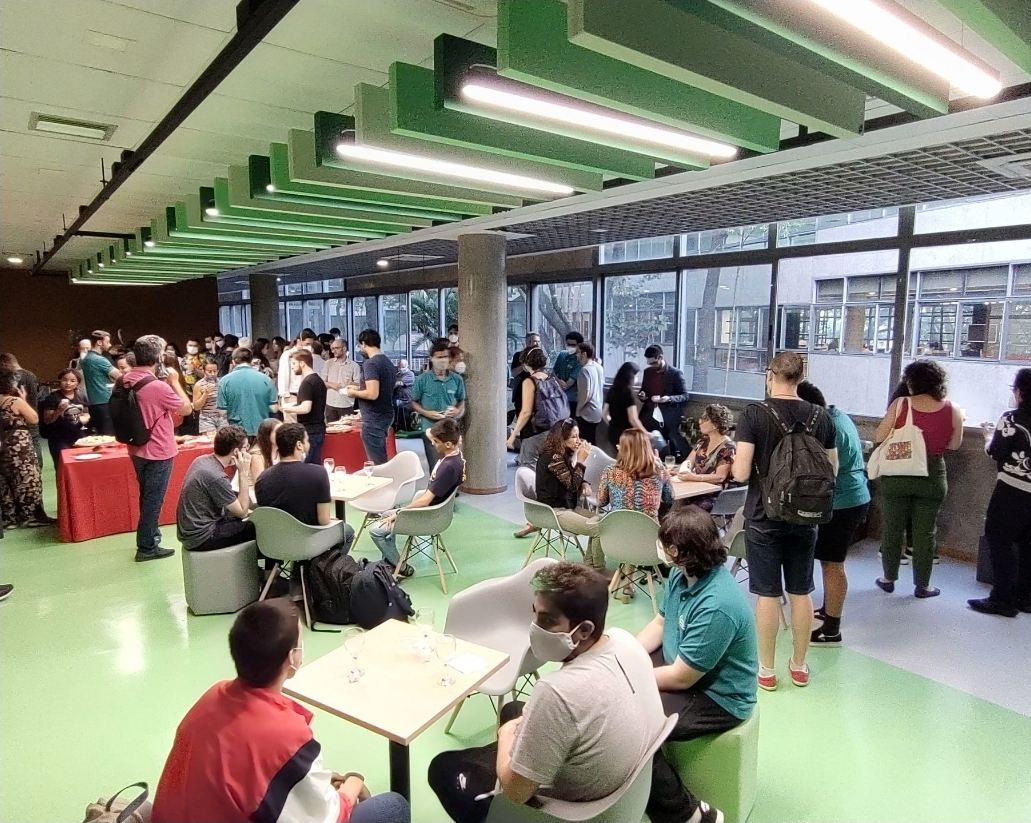
\includegraphics[width=0.6\textwidth]{figuras/cap.1/Screenshot_20260430_160250_Chrome.jpg}
\caption[Café após a Tech Hour do C4AI realizada em 23 de março de 2022, no InovaUSP, primeiro ano do trabalho de campo desta pesquisa.]{Café após a \textit{Tech Hour} do C4AI realizada em 23 de março de 2022, no InovaUSP, primeiro ano do trabalho de campo desta pesquisa. Eu apareço em primeiro plano, de costas, com jaqueta vermelha, em conversa com outros dois pesquisadores de graduação do Centro. A imagem registra um dos primeiros encontros presenciais do C4AI após a pandemia. Foi extraída do site do C4AI, disponível em: \protect\url{https://c4ai.inova.usp.br/about.html\#difusao}. Acesso em: 30 abr. 2026. No intervalo de café após a \textit{Tech Hour} (como são chamadas as apresentações de pesquisa presenciais no C4AI, também transmitidas no YouTube), comecei a conhecer alguns dos pesquisadores do Centro. Lembro-me do contexto em que a foto foi tirada e, por isso, consegui buscar no meu caderno de campo a data exata e uma observação importante que registrei sobre a conversa com eles. Perguntaram-me o que eu fazia no C4AI, presumindo que eu fosse da ciência da computação ou de áreas afins, e expliquei que estava ali para estudar o que eles faziam em um centro de inteligência artificial. Com um tom de descoberta, um deles me disse que \protect\enquote{eles} seriam, então, o meu objeto de pesquisa. Concordei. Para eles, era assim que se fazia ciência. Fiquei alguns dias pensando sobre essa conversa, dúvida que o capítulo~\ref{capitulo1} retoma ao tratar dos modos pelos quais os cientistas da computação reconhecem, ou não, as ciências sociais como interlocutoras legítimas. Essa fotografia foi registrada pelo próprio Centro e, ao consultar o site do C4AI tempos depois, descobri que apareço nela, provavelmente fotografada um pouco depois de essa conversa ter acontecido. Uma outra feliz coincidência.}
\label{fig:tech-hour-c4ai}
\end{figure}

   % Apresentação / Introdução (Será a página 1 oficial)
\renewcommand{\textbf}[1]{#1}

\chapter{Onde está o laboratório e os seus cientistas?}
\label{capitulo1}

\epigrafe{%
A Pesquisa é a zona para a qual são arrastados humanos e não humanos, onde ao longo das eras foi feito o mais extraordinário dos experimentos coletivos para distinguir, em tempo real, o ``cosmos'' da ``desordem'' sem que ninguém, cientista ou ``estudioso da ciência'', pudesse saber de antemão qual seria a resposta provisória. Talvez, afinal das contas, os estudos de ciência sejam Anticiência.}%
{Bruno Latour, \textit{A ciência em ação: como seguir cientistas e engenheiros sociedade afora}, 2011.}

Antes de entrar em campo, situo o leitor sobre o que vai encontrar neste capítulo~\ref{capitulo1}. Parto de uma pergunta, onde está o laboratório dos pesquisadores de inteligência artificial e onde estão os seus cientistas, e a desdobro em três gestos analíticos que organizam o capítulo: o corte que delimita uma rede que de outro modo se daria a ver como infinita, a descrição das existências parciais que se compõem comigo e com a inteligência artificial generativa na feitura da tese, e a compostagem que põe a fermentar materiais que o desenho da pesquisa mantinha separados. Ao longo do percurso defino o conceito de tecno-etnografia que dá nome ao trabalho inteiro, sustento a figuração têxtil do método pelo \textit{patchwork}, e fecho o capítulo com a relação entre as duas figurações que constituem esta tese, a têxtil e a topológica, e com a questão que ela me deixou em aberto. A linha do tempo e o mapa que abrem o capítulo dão a ver, antes da leitura, esse percurso e as suas condições. A linha do tempo (Figura~\ref{fig:linha-tempo-cap1}) inscreve, num diagrama de Gantt, os fatos que correm por baixo da pesquisa ao longo de uma década, das condições tecnológicas, sanitárias, regulatórias e bibliométricas às etnográficas, das quais só as últimas se tornam texto enquanto as demais permanecem como condição de possibilidade. O mapa do capítulo (Figura~\ref{fig:mapa-cap1}) dá a ver a arquitetura argumentativa: os fundamentos etnográficos na base, os quatro movimentos em que desdobro os três gestos analíticos, com a matriz dos cortes que cada capítulo da tese faz, e as relações que ligam um movimento ao seguinte. Os dois pertencem ao registro da inscrição, e dão à visão, numa superfície plana, o que penso e teço na espessura do argumento.

Em dezembro de 2022, estive no México para participar do congresso da \textit{Society for Social Studies of Science} (4S), onde apresentei pela primeira vez os resultados preliminares desta pesquisa. Além da experiência de conhecer o país e participar de um evento internacional na área de estudos sociais da ciência e tecnologia, viajei com um grupo diverso de pesquisadores e amigos que contribuíram para aprofundar a reflexão sobre o que significa fazer ciências sociais e investigar como a ciência é produzida em outros áreas do conhecimento. Clarissa, uma das companheiras da viagem e do doutorado na Unicamp, investigava um tema muito diferente sobre o trabalho de antropólogas que menstruam em campo. Ainda assim, compartilhávamos uma preocupação: a ideia de ``não ferir os sentimentos estabelecidos'', uma reflexão de Isabelle Stengers,\footnote{Stengers propõe em \textit{Another Science is Possible} uma ``ciência lenta'' (\textit{slow science}) como resistência às pressões de produtividade que degradam a qualidade do pensamento científico \parencite{stengers2018another}. A defesa da lentidão pressupõe condições de autonomia que nem sempre são possíveis. Esta tese documenta como a temporalidade acadêmica pode se tornar condição de vulnerabilidade quando articulada às lógicas temporais corporativas. Enquanto universidades públicas operam em horizontes de décadas, corporações decidem em ciclos de curto prazo segundo lógicas de retorno sobre investimentos. A capa da edição inglesa traz um caracol, imagem que ressoa com o lema zapatista ``lento, pero avanzo'' e que esta tese adota na dedicatória.} ``como estratégia para criar alianças com interlocutores cientistas, engenheiros e áreas afins''. Longe de se configurar como atitude conformista, trata-se justamente do oposto: ``uma postura calcada apenas no confronto e na denúncia das mazelas da tecnociência é infrutífera, pois produz um resultado alienante e perverso: oculta para nós, pessoas que pesquisam desde as ciências humanas, nossa responsabilidade enquanto coabitantes desse mesmo espaço onde estão os cientistas que denunciamos'' \parencite[p. 314]{costa2024manchando}. Isso não significa que as denúncias sejam irrelevantes, mas ``reconhecer nossa responsabilidade como coabitantes do sistema de produção de conhecimento científico é também aprender a construir e sustentar diálogos, por mais difíceis que sejam'' \parencite[p. 314]{costa2024manchando}.\footnote{Costa desenvolve o conceito de \textit{armadilha} como estratégia metodológica e política para que corpos marcados produzam conhecimento crítico dentro de estruturas acadêmicas sem serem devorados por elas. A armadilha opera em duas etapas, primeiro, encanta através da beleza estética; depois, revela que as imagens fractais são feitas de sangue menstrual, vazando questões feministas de forma que não sejam imediatamente rejeitadas. A etnografia também pode operar como armadilha. Seguir os atores sem julgamento prévio, ganhar confiança, descrever o que é dito e feito para depois tornar visíveis tensões e contradições que os próprios atores não nomeiam \parencite{costa2024manchando}.}

Quase três anos depois do congresso no México, em novembro de 2025, a IBM fechou seu laboratório de pesquisa no Brasil, o único da América Latina, operando há 15 anos com mais de 100 pesquisadores. Em dezembro de 2025, encerrou-se o convênio \texttt{C4AI-IBM}.\footnote{Adoto nesta tese a convenção tipográfica de marcar em fonte monoespaçada, via comando \texttt{\textbackslash texttt\{\}} do \texttt{LaTeX}, três famílias de nomes próprios técnicos: plataformas, linguagens de programação e ambientes computacionais que medeiam a escrita desta tese (\texttt{Python}, \texttt{LaTeX}, \texttt{Overleaf}, \texttt{GitHub}, \texttt{claude code}, \texttt{claude.ai}, \texttt{MermaidChart}, \texttt{NotebookLM}); siglas institucionais de centros, projetos e instituições que compõem o campo de pesquisa (\texttt{C4AI}, \texttt{NLP2}, \texttt{GrIA}, \texttt{USP}, \texttt{FAPESP}, \texttt{IBM}, \texttt{Unicamp}, \texttt{SciELO}, \texttt{Capes}); e nomes próprios de sistemas, modelos e corpora de inteligência artificial (\texttt{Spira}, \texttt{Carolina}, \texttt{Sabiá}, \texttt{claude}, \texttt{GPT}, \texttt{BERT}). A marcação não é questão de estilo. Em coerência com o que sustento sobre figurações como tropos materiais-semióticos no sentido proposto por Donna Haraway, a fonte monoespaçada permanente mantém visível, em toda página do texto, que cada um desses nomes próprios designa um ponto de mediação técnica com agência sobre o que vejo, leio, escrevo e descrevo. A distinção tipográfica entre o redondo, reservado aos nomes próprios de pessoas humanas (Marcelo Finger, Bruno Latour, eu), e a fonte monoespaçada, reservada aos nomes próprios técnicos, recusa a homogeneização tipográfica que apagaria a heterogeneidade dos atores que compõem a rede sociotécnica desta pesquisa.} Desde o início desta pesquisa eu me perguntava até quando aquilo duraria. Na época, havia expectativa por parte do \texttt{C4AI} de que se estendesse por dez anos. Acabou em cinco. A confiança com que meus interlocutores falavam sobre a participação da \texttt{IBM} e a solidez dos investimentos exemplifica de um modo brutal a ``economia especulativa de promessas'' que Stengers critica \parencite{stengers2018another}. Eu, no entanto, repetia para mim mesma: é uma empresa, quero dizer, funciona através de lógicas muito distintas das da universidade. 

Eu já estava na fase final da escrita desta tese quando o convênio foi encerrado, e isso obrigou-me a rever algumas questões que atravessam esta pesquisa. No entanto, acabou por ser também um presente etnográfico sobre o registro de uma parceria público-privada controversa, tensa, contraditória e, a seu modo, bem-sucedida na pesquisa em IA em uma universidade pública brasileira. Essa situação me aproximou do estudo de \textcite{Latour1993Aramis} sobre o Aramis, um sistema de transporte que nunca chegou a existir. Latour fez sua pesquisa entre dezembro de 1987 e janeiro de 1989 com o intuito de investigar por que o projeto havia sido cancelado em fevereiro de 1987.\footnote{Minha posição temporal distingue-se: iniciei a pesquisa em março de 2022, quando a parceria parecia consolidada; o encerramento em dezembro de 2025 não estava previsto. Registrei processos enquanto ocorriam, capturando tensões que permaneciam latentes porque a rede ainda resistia.} Tanto o Aramis quanto o \texttt{C4AI} são casos de parcerias público-privadas onde atores com interesses diversos mobilizam promessas de longo prazo que se desfazem quando cálculos estratégicos corporativos mudam. Em fevereiro de 1987, a Matra distribuiu uma nota ordenando ``pare tudo''; em agosto de 2025, a \texttt{IBM} comunicou internamente que o convênio não seria renovado. No Aramis, a retirada resultou no cancelamento completo após quase vinte anos de investimentos públicos.\footnote{O que restou do Aramis foi um protótipo no saguão da empresa, uma casca vazia sem trilhos, sem eletricidade, sem passageiros: ``um objeto de museu'' antes mesmo de ter sido um objeto no mundo. Latour pergunta quando uma tecnologia se torna um objeto. ``Nunca'', ele responde, ``exceto quando porções extraídas da instituição são colocadas em exposição dentro de museus técnicos'' \parencite[p. 9]{Latour1993Aramis}. É só no ferro-velho que um objeto técnico finalmente se torna objeto. Antes disso, é sempre uma instituição, uma rede de humanos e não humanos, uma transação em curso. Law radicaliza esse argumento ao propor vocabulário para pensar objetos que nunca alcançam fechamento, investigando ``as vidas incertas e complexas dos objetos em um mundo onde não há fechamento'' \parencite[p. 59]{Law2004After}. Objetos são múltiplos mesmo quando parecem singulares, e essa multiplicidade persiste sem se resolver com estabilização.}
No \texttt{C4AI}, a saída da \texttt{IBM} não acabou com o Centro, mas forçou sua reconfiguração como a perda de financiamento corporativo, incertezas sobre projetos em andamento e o esvaziamento das expectativas construídas ao longo de cinco anos. O Centro continua a existir, mas a parceria \texttt{IBM}-\texttt{C4AI} tornou-se objeto do passado; uma relação que deixou rastros em artigos científicos, infraestrutura computacional e promessas não cumpridas. Esta tese começou como uma etnografia de um arranjo sociotécnico aparentemente estável e terminou descrevendo justamente a sua instabilidade e mudanças em um campo volátil e de difícil acesso, e o que isso pode vir a dizer sobre a pesquisa pública em IA no Brasil.

Em 2016, uma cena que circulou amplamente pela internet tornou-se uma das imagens de referência da história recente da inteligência artificial: Jensen Huang, presidente da Nvidia, entrega a Elon Musk, então cofundador da \texttt{OpenAI}, o primeiro supercomputador DGX-1, e Musk assina o chassi da máquina.\footnote{A cena foi registrada em fotografia compartilhada pelo próprio Musk no Twitter, plataforma que viria a adquirir em 2022 e renomear como X, e circulou amplamente desde então. O DGX-1, entregue no escritório da \texttt{OpenAI} em São Francisco, foi avaliado em US\$~129.000 e reunia oito GPUs Tesla P100 com capacidade de até 170 teraflops (FP16), tornando-se a primeira infraestrutura de computação dedicada exclusivamente ao treinamento de redes neurais em escala. Ao fundo da fotografia, uma inscrição parcialmente legível na parede anuncia que o destino do mundo depende do uso que se faz do conhecimento. Opto por não reproduzir a imagem nesta tese e por descrever a cena, em coerência com a economia de figuras que adoto no capítulo. Fonte: Twitter/@elonmusk, 2016.} Menos de uma década depois, a arquitetura de treinamento inaugurada por aquela máquina produziria sistemas capazes de gerar texto, imagem, código e voz com fluência suficiente para redesenhar mercados de trabalho, práticas científicas, sistemas educacionais e disputas geopolíticas. Treinar esses sistemas exige acesso a dezenas, centenas ou milhares de GPUs; a infraestrutura que a cena de 2016 inaugura tornou-se condição de entrada para qualquer laboratório que pretenda produzir modelos competitivos, e a busca por mais poder computacional e mais dados funcionou, por anos, como lei não escrita do desenvolvimento de modelos de linguagem. Em janeiro de 2026, o lançamento do \textit{DeepSeek}, modelo chinês que atingiu desempenho comparável aos sistemas americanos de ponta com apenas uma fração dos recursos computacionais e dos dados, abalou esse paradigma e reabriu a questão sobre quais são, afinal, as condições necessárias para fazer pesquisa em IA. O \texttt{Spira}, projeto desenvolvido no laboratório de processamento de linguagem natural do IME-USP antes mesmo de o \texttt{C4AI} existir como instituição, chegou a essa condição por outra via através de uma doação pontual de GPU da própria Nvidia, registrada nos agradecimentos do primeiro artigo do projeto \parencite{Casanova2021DeepLearning}, sem contrato nem vínculo institucional. O \texttt{C4AI}, por sua vez, manteve ao longo de cinco anos um cluster de GPUs financiado pela USP-Fapes-IBM; em dezembro de 2025, dias após o fim da parceria com a \texttt{IBM}, a USP inaugurou o JAIRU, o maior \textit{cluster} (conjunto de GPUs que trabalham em paralelo) de IA da América Latina, com 96 GPUs Nvidia B200 e um investimento de aproximadamente R\$~40 milhões. As possibilidades que se abriram com aquela máquina são inseparáveis dos problemas que trouxeram, a concentração de poder computacional em poucas corporações, a dependência infraestrutural de países periféricos, a extração de trabalho não remunerado de milhões de usuários cujos dados alimentam os modelos, a opacidade dos sistemas e dificuldade de responsabilização quando erram, entre outros problemas. 

Esta etnografia foi feita durante esses acontecimentos. Iniciei o trabalho de campo no \texttt{C4AI} em março de 2022, seis meses antes do lançamento do \texttt{ChatGPT}, quando a inteligência artificial generativa ainda era objeto de especialistas e o debate público sobre seus efeitos mal havia começado. Entre março de 2022 e dezembro de 2025, assisti, dentro e a partir do Centro, à aceleração que converteu modelos de linguagem em infraestrutura cotidiana, ao crescimento das publicações sobre processamento de linguagem natural pelo \texttt{C4AI}, ao surgimento do primeiro modelo de linguagem brasileiro, à aprovação do primeiro marco regulatório global e ao encerramento da parceria que havia dado origem ao campo que eu estudava. O \texttt{C4AI}, fundado quatro anos depois do DGX-1 com recursos públicos brasileiros e co-financiado pela \texttt{IBM}, é um nó nessa rede e herdeiro das possibilidades, limites e todo o tipo de problema que a fotografia de Jensen Huang e Elon Musk evoca. Acompanhar esse Centro por quase quatro anos é também acompanhar uma pergunta que a fotografia enseja: qual é o papel da universidade pública na produção de conhecimento em inteligência artificial quando quem está nas fronteiras da pesquisa em IA são essas mesmas corporações? Esta tese documenta uma tentativa de resposta situada à essa questão: o que o \texttt{C4AI} fez, como se organizou e o que ficou quando a \texttt{IBM} deixou de co-financiar o centro. 

\begin{figure}[htbp]
  \centering
  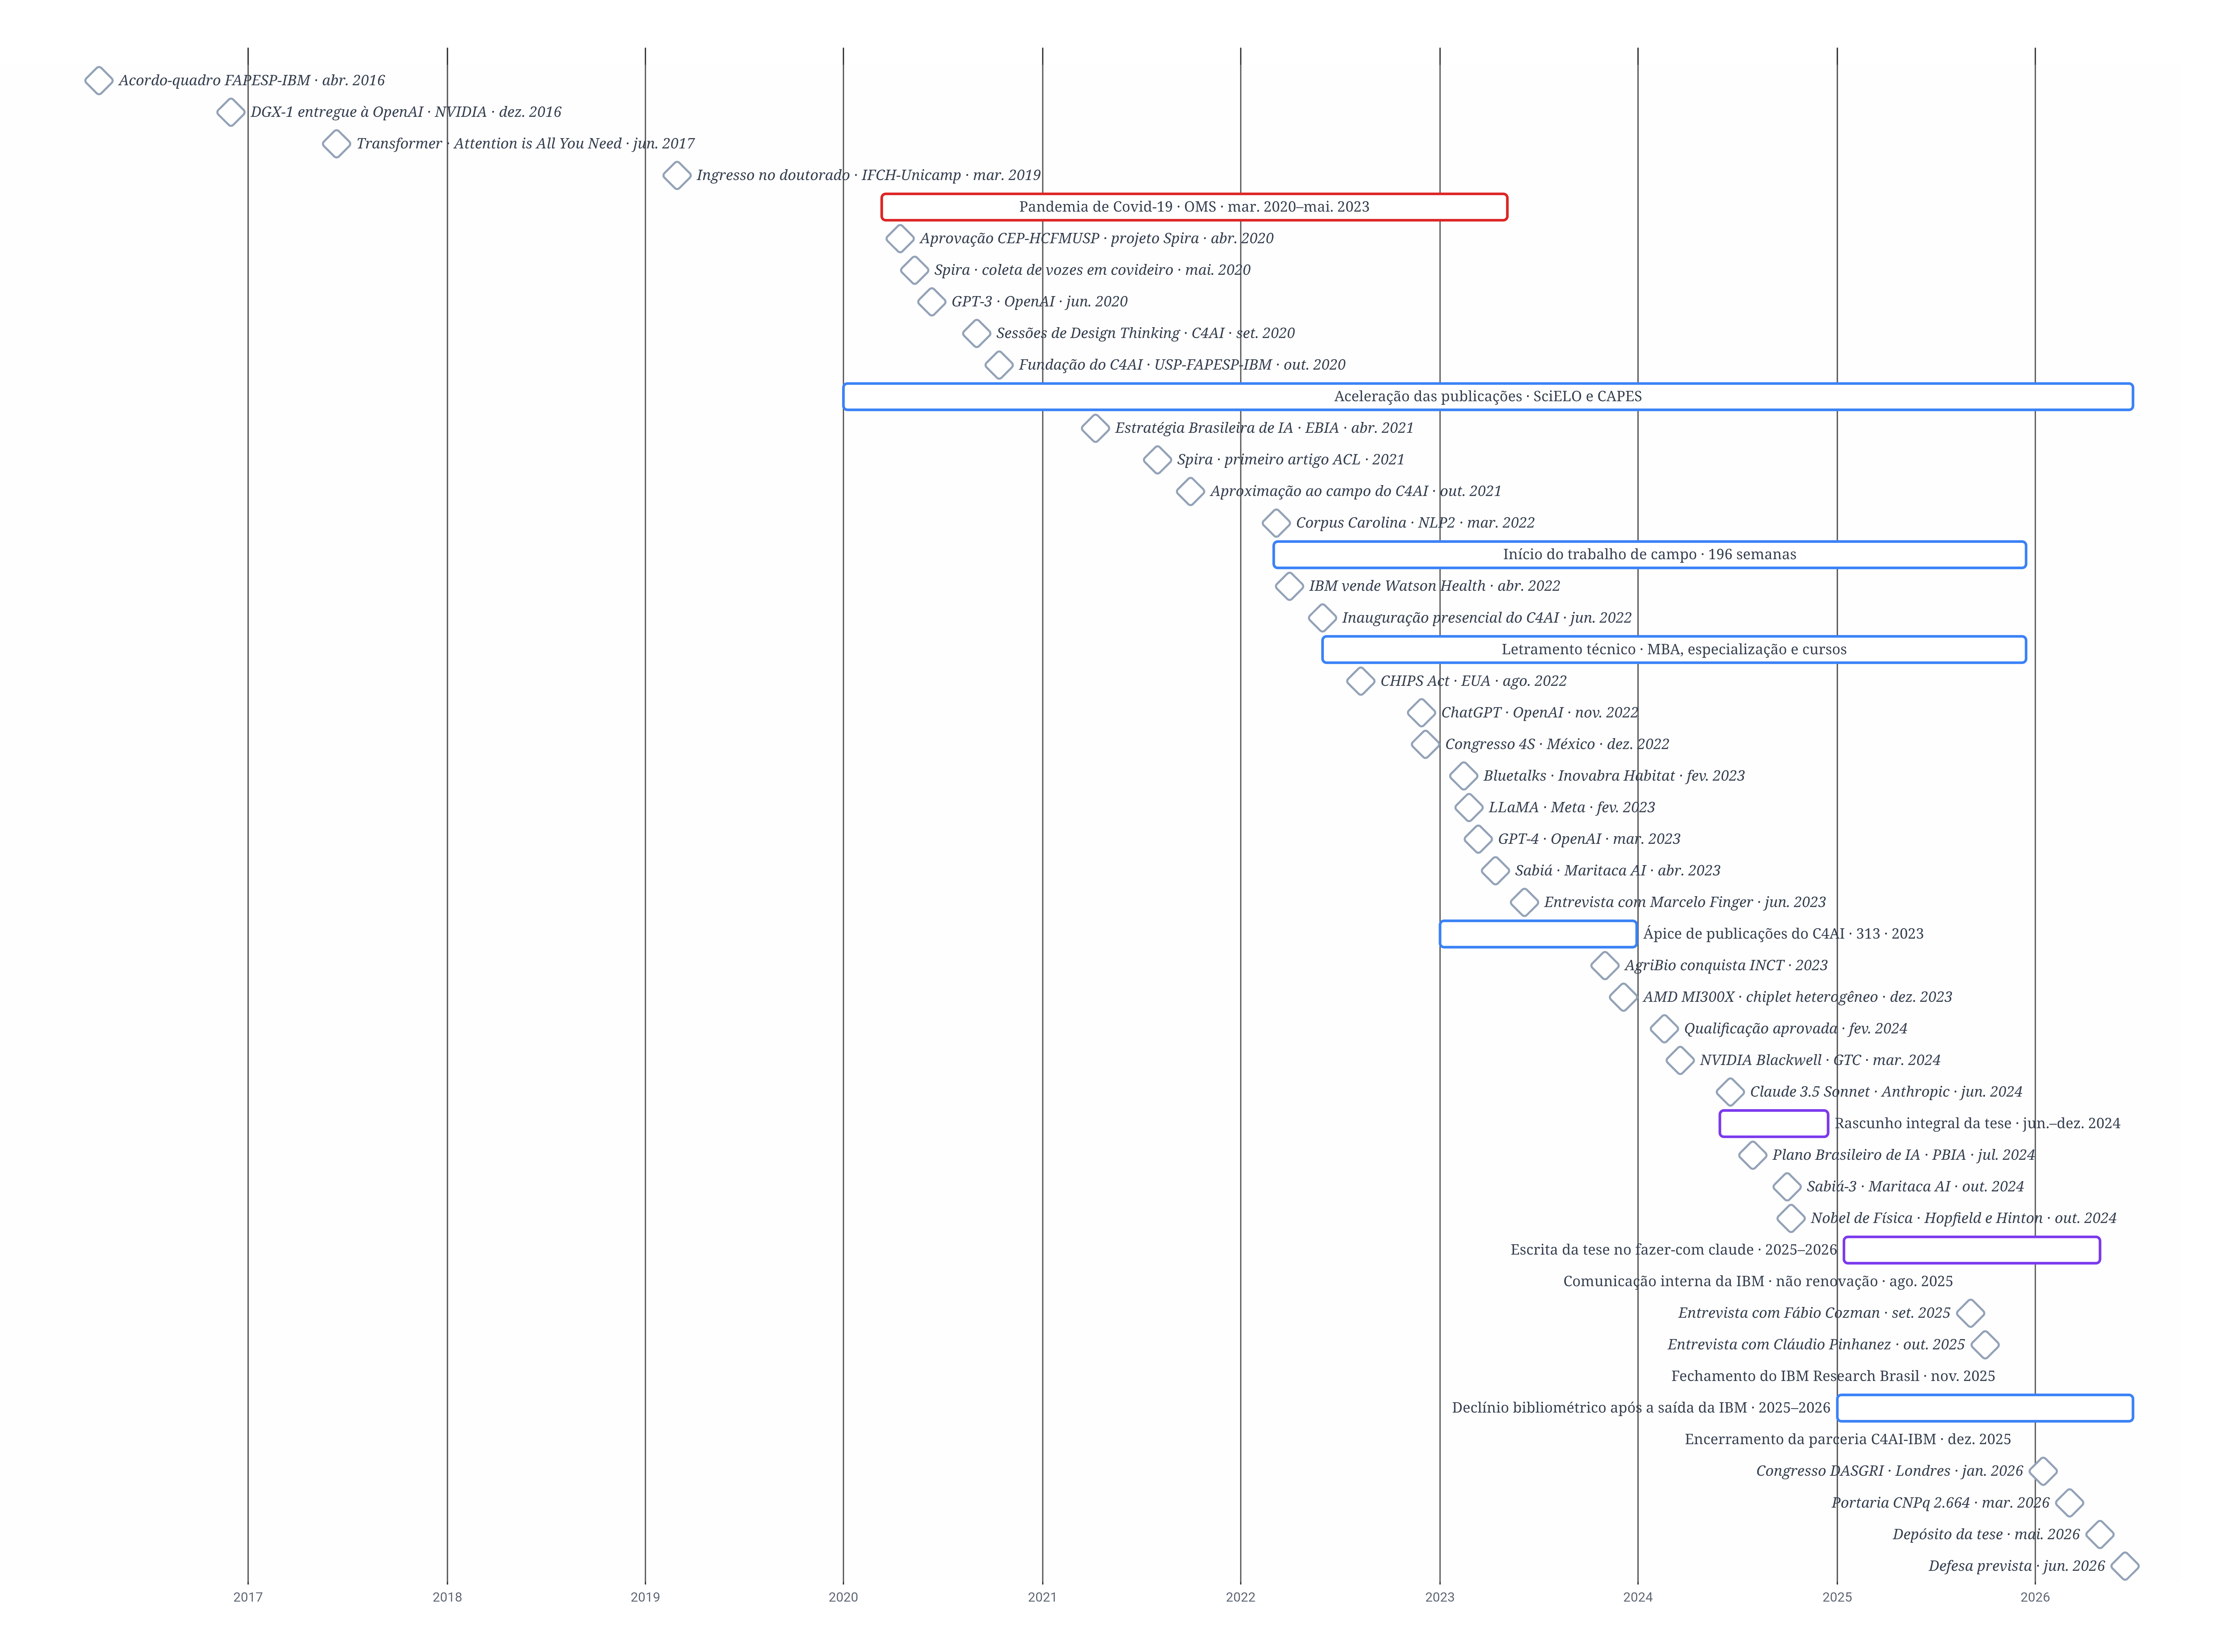
\includegraphics[width=0.7\textwidth,keepaspectratio]{figuras/cap.1/linha-tempo-capitulo1.png}
  \caption[Linha do tempo do capítulo~\ref{capitulo1}]{\textbf{Linha do tempo do capítulo~\ref{capitulo1}: condições materiais, sanitárias, regulatórias, bibliométricas e etnográficas em que se fez esta pesquisa.} Esta linha do tempo dá a ver, numa superfície plana, os fatos que correm por baixo do texto da tese, dispostos em sequência ao longo de uma década, e pertence ao registro da inscrição, no sentido de \textcite{Latour1986Visualization}. Leio-a, em diálogo com \textcite{Law2004After}, como o \textit{hinterland} que sustenta o que aparece como presença no texto: a maior parte desses fatos permanece como condição de possibilidade, e só os do trabalho de campo se tornam texto. Atravessam a cronologia as condições \textit{tecnológicas}, da aceleração da infraestrutura computacional para IA entre 2016 e 2026, do DGX-1 entregue à \texttt{OpenAI} à arquitetura Blackwell da NVIDIA, e dos modelos que cruzaram minha pesquisa, GPT-3, \texttt{ChatGPT}, GPT-4, LLaMA, Sabiá e Sabiá-3 da \texttt{Maritaca AI}, o \texttt{claude} 3.5 Sonnet e modelos da família Opus, com o Nobel de Física de 2024 para Hopfield e Hinton; as \textit{sanitárias}, da pandemia de Covid-19 entre março de 2020 e maio de 2023, condição de possibilidade do \texttt{Spira}, que coletou vozes em covideiro, e do \texttt{C4AI}, fundado em outubro de 2020, em plena pandemia; as \textit{regulatórias}, da aprovação ética do CEP-HCFMUSP para o \texttt{Spira} em abril de 2020 às políticas científicas brasileiras de fomento à IA (EBIA 2021, PBIA 2024), aos arranjos internacionais que reposicionaram o setor (CHIPS Act, AI Act) e à Portaria CNPq 2.664 de 2026, que minha tese antecipou por escolha metodológica; as \textit{bibliométricas}, da aceleração das publicações em IA nas ciências humanas brasileiras (SciELO, CAPES) entre 2020 e 2026, com o ápice de 313 publicações do \texttt{C4AI} em 2023 e o declínio associado à saída da \texttt{IBM} em 2025-2026; e as \textit{etnográficas}, os fatos que se tornam texto na tese, do acordo-quadro Fapesp-IBM de 2016 ao meu ingresso no doutorado em 2019, à fundação do \texttt{C4AI} em outubro de 2020, à minha aproximação ao campo em outubro de 2021, às 196 semanas de trabalho de campo entre março de 2022 e dezembro de 2025, ao letramento técnico acumulado em paralelo, ao rascunho integral da tese redigido entre junho e dezembro de 2024 sem assistência de inteligência artificial, ao fazer-com \texttt{claude} e à \textit{skill} \texttt{juliane-dissertacao} entre janeiro de 2025 e maio de 2026, às três entrevistas com Marcelo Finger, Fábio Cozman e Cláudio Pinhanez, e aos dois eventos que abriram a caixa-preta institucional na finalização da pesquisa, o fechamento da \texttt{IBM} Research Brasil em novembro de 2025 e o encerramento da parceria \texttt{C4AI}-\texttt{IBM} em dezembro de 2025. Inscrição que produzi no fazer-com \texttt{claude} (\texttt{Anthropic}) e hospedei no \texttt{MermaidChart}\footnote{Versão interativa do diagrama disponível em: \url{https://mermaid.ai/d/b27ca78c-b037-42fe-a3eb-939a092e1455}. Acesso em: \today.}, em que os fatos que o texto principal precisou deixar fora para sustentar seu fluxo narrativo se dispõem, todos, numa só superfície. Esta linha do tempo é o par do mapa do capítulo (Figura~\ref{fig:mapa-cap1}): onde o mapa inscreve a estrutura argumentativa do capítulo, a linha do tempo inscreve as condições materiais que correm por baixo dela.}
  \label{fig:linha-tempo-cap1}
\end{figure}

\begin{figure}[htbp]
  \centering
  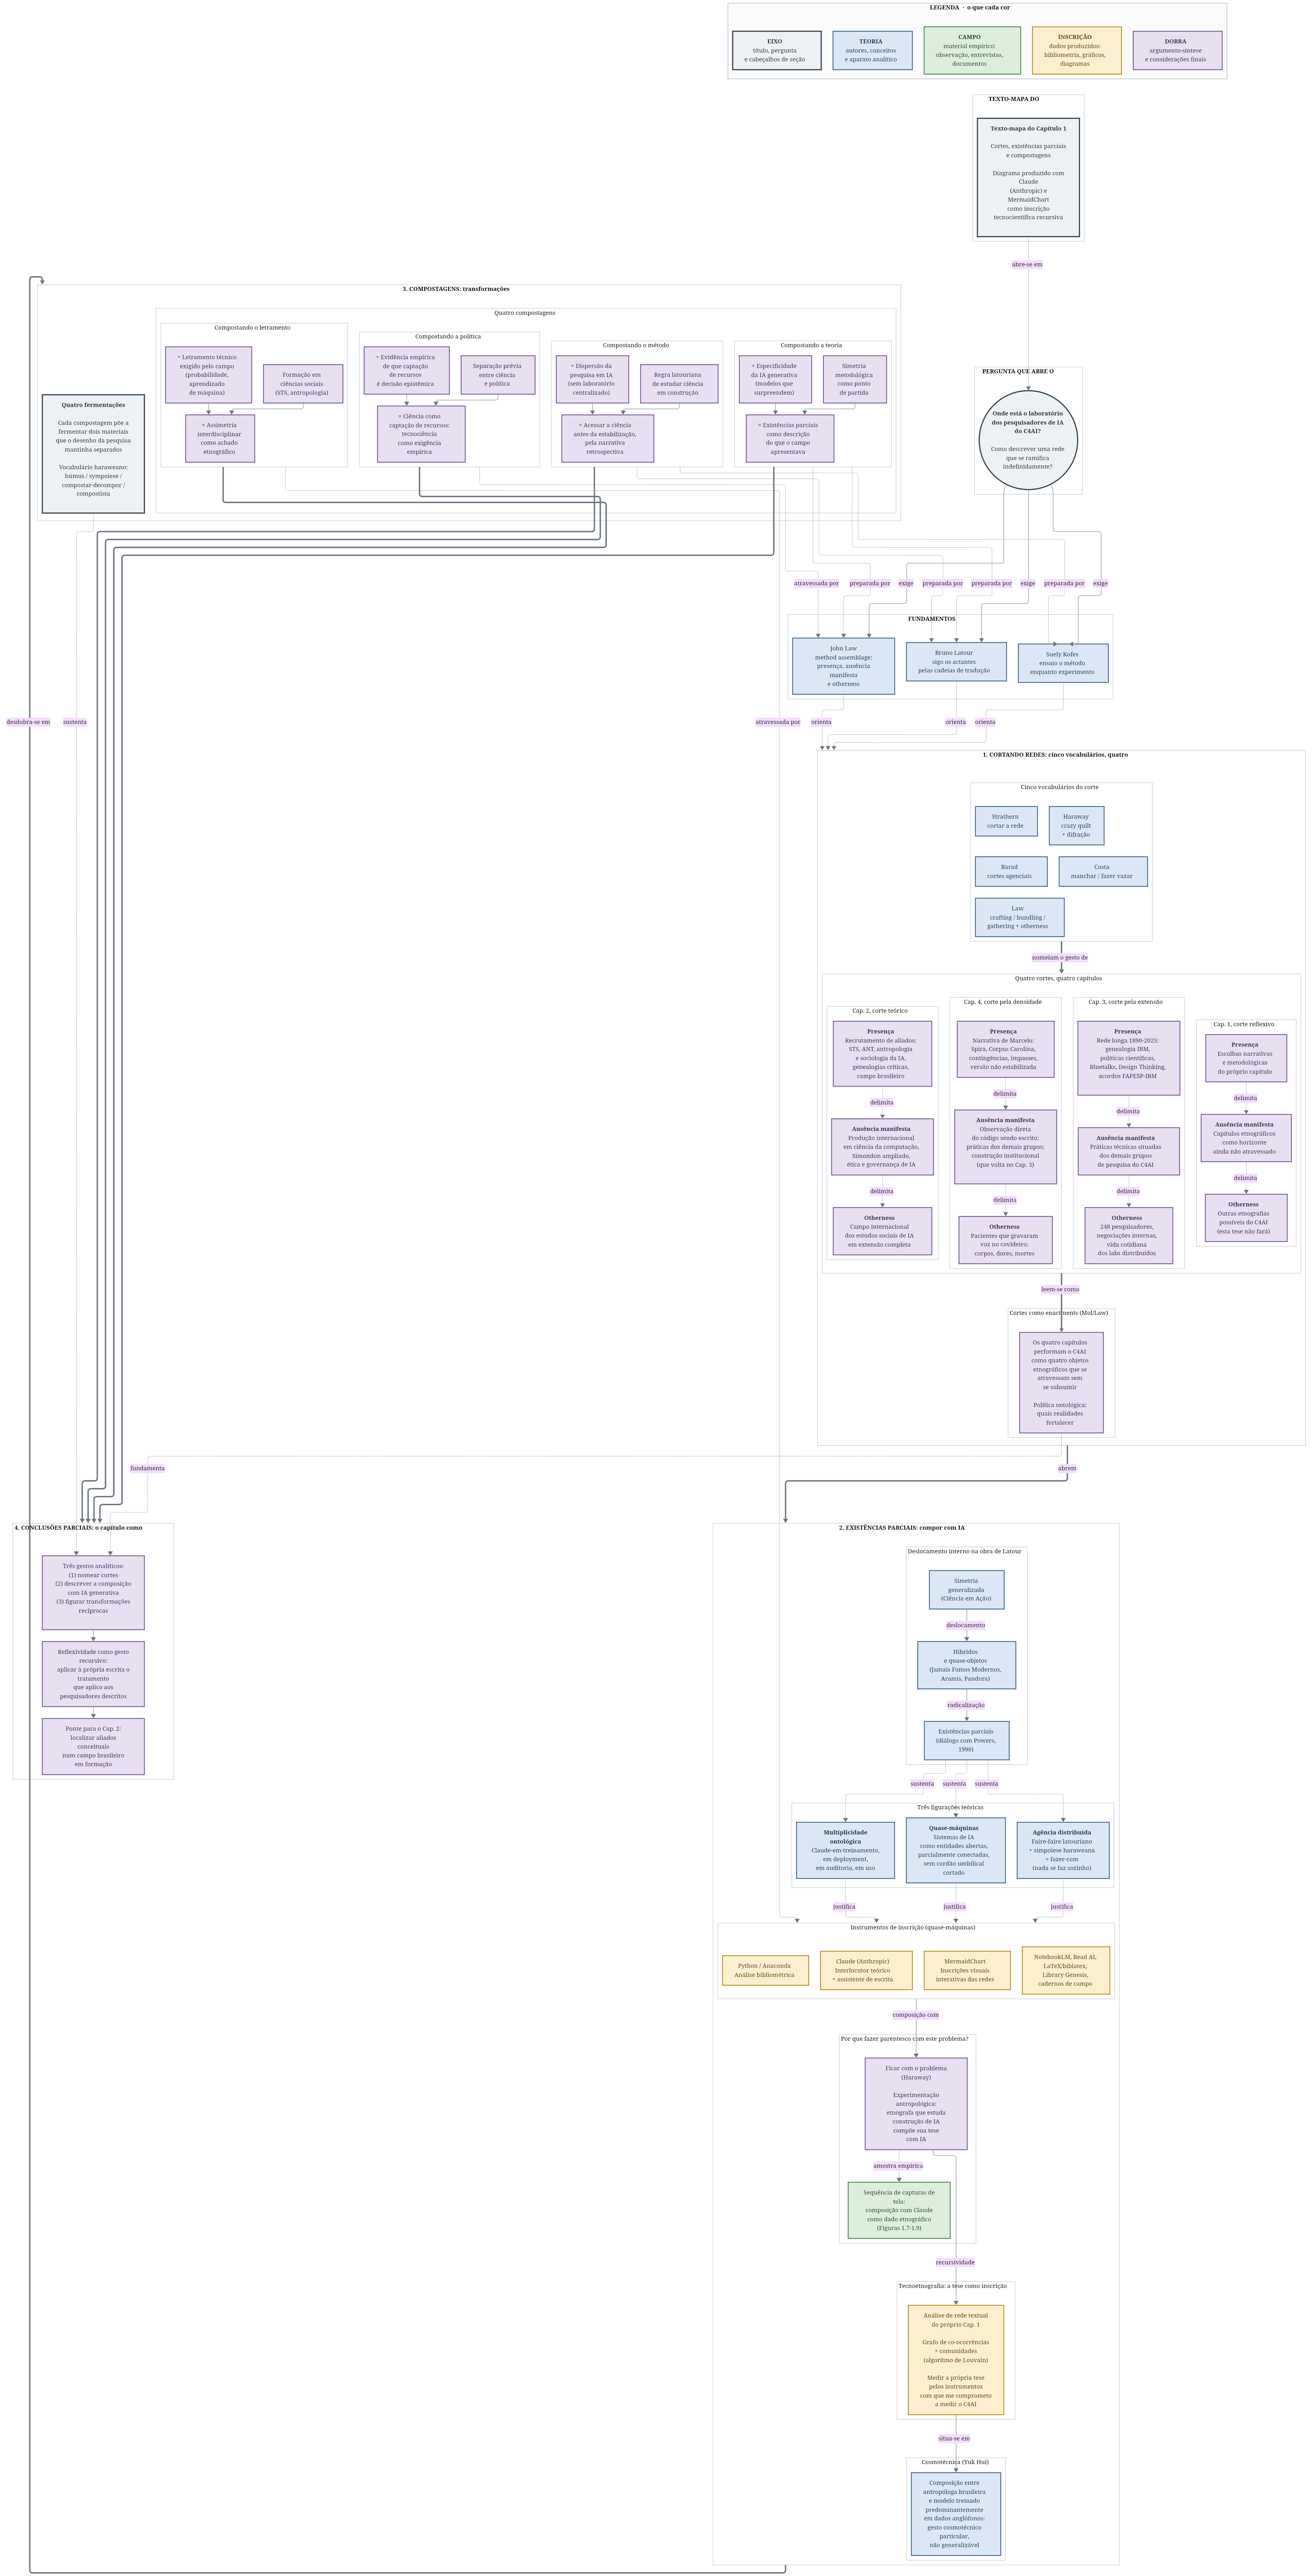
\includegraphics[width=0.4\textwidth]{figuras/cap.1/mapa-capitulo1-v2.png}
  \caption[Mapa do capítulo~\ref{capitulo1}]{\textbf{Mapa do capítulo~\ref{capitulo1}: a arquitetura argumentativa, da pergunta inicial às conclusões parciais.} Este mapa situa o leitor na arquitetura do capítulo, ao dar a ver numa superfície plana os fundamentos etnográficos que o sustentam, os quatro movimentos em que desdobro os três gestos analíticos, e as relações que ligam um movimento ao seguinte. Na base, três fundamentos sustentam o restante: \textcite{Kofes2015Maconaria}, para quem o método se ensaia enquanto se experimenta, \textcite{Latour2011CienciaEmAcao}, que pede para seguir os actantes, e \textcite{Law2004After}, com o \textit{method assemblage} que produz presença, ausência manifesta e \textit{otherness}. O primeiro movimento, \textit{Cortando redes}, reúne o corte de Strathern e conceitos vizinhos de Barad, Haraway, Costa e Law e a matriz dos quatro cortes que cada capítulo da tese faz, descrito cada um pela tríade presença/ausência manifesta/\textit{otherness}, e que se leem como \textit{enactments} no sentido praxiográfico de \textcite{mol2002body} e \textcite{Law2004After}. O segundo, \textit{Existências parciais}, parte de um deslocamento interno na obra de Latour, do princípio de simetria aos híbridos e às existências parciais, e sustenta três figurações teóricas (quase-máquinas, agência distribuída e a multiplicidade ontológica de Claude), que justificam o trabalho dos instrumentos de inscrição com que componho a tese e a análise de rede textual do próprio capítulo como gesto recursivo, situados como gesto cosmotécnico particular (Hui). O terceiro, \textit{Compostagens}, nomeia quatro fermentações específicas, do método, da teoria, do letramento e da política, cada uma como soma de duas matérias que o desenho da pesquisa mantinha separadas. As \textit{Conclusões parciais} reúnem os três gestos analíticos, registram a reflexividade como gesto recursivo e abrem a ponte para o capítulo~\ref{capitulo2}. A inscrição é, ela mesma, parte do que descreve: produzi-a com o \texttt{claude} (\texttt{Anthropic}) e hospedei-a no \texttt{MermaidChart}\footnote{Versão interativa do diagrama disponível em: \url{https://mermaid.ai/d/6dbd9e0b-a652-428d-99b1-a76d0c068b5b}. Acesso em: \today.}, em cadeia de traduções entre minha descrição verbal das relações argumentativas do capítulo e o código \textit{Mermaid} executado pelo modelo. A inscrição funciona, nos termos de \textcite{Latour1986Visualization}, como móvel imutável que torna combinável em superfície plana o que o texto desdobra ao longo de dezenas de páginas, e nos termos de \textcite{Law2004After}, como redução produtiva que perde riqueza empírica e ganha capacidade de fazer conexões.}
  \label{fig:mapa-cap1}
\end{figure}

Estar no campo durante esse período implicou um desafio que vai além do habitual esforço de atualização bibliográfica. Nas seções que se seguem, detalho os fundamentos teórico-metodológicos que orientaram essa trajetória, as operações de triangulação que permitiram articular dados heterogêneos, os cortes analíticos estratégicos que transformaram redes infinitas em objetos etnográficos analisáveis, e as quatro lições que o encontro entre teoria e campo produziu como contribuições metodológicas desta tese. A etnografia, como o caracol, avançou devagar, secretando seu rastro. O que esse rastro deixou está escrito (e inscrito) nesta tese. Mas, esse rastro também deixa meus vestígios enquanto pesquisadora aprendendo a caminhar sobre superfícies estranhas, e deixa, sobretudo, os vestígios dos próprios pesquisadores do \texttt{C4AI} construindo redes, mobilizando inscrições e recrutando aliados, negociando com corporações, fazendo, por fim, \textit{tecnociência}.\footnote{Em \textit{Ciência em Ação}, \textcite{Latour2011CienciaEmAcao} nomeia com esse termo o campo em que ciência e tecnologia se produzem como um só processo, sem partição prévia entre fatos e artefatos. \textcite{stengers2018another} o toma em outra direção, a da \textit{fast science}, e renomeia a economia do conhecimento como \textit{economia especulativa de promessas}.}

Para Latour, a tecnociência é prática coletiva de fechamento de caixas-pretas, em que as controvérsias se resolvem pela capacidade de estender redes em extensão e em densidade, nas quais teoremas, máquinas, documentos, financiamentos e alianças institucionais tornam o custo da discordância proibitivo para o oponente. Stengers descreve a forma que as práticas científicas assumem quando recrutadas pela lógica industrial e pelos imperativos de competitividade, em que a formação do pesquisador funciona como anestesia que o torna insensível à recalcitrância dos mundos atravessados pela pesquisa, e em que a avaliação crítica entre pares se enfraquece porque ninguém quer cortar o galho da promessa que sustenta o campo. Latour e Stengers descrevem dimensões diferentes do mesmo fenômeno: os conceitos latourianos de rede e de translação permitem mapear como redes tecnocientíficas se estendem e se estabilizam; o diagnóstico de Stengers expõe como essas redes, sob condições contemporâneas, vivem regimes específicos de captura, aceleração e despolitização. Sustento esta tese nos dois registros. O que me interessa na proposta de Stengers é que ela articula, ao mesmo tempo, a crítica, que não se reduz à denúncia, e a construção de alianças. A trajetória da parceria \texttt{C4AI}-\texttt{IBM}, com a promessa inicial de dez anos reduzida a cinco quando os cálculos corporativos se reorganizaram, é caso empírico em que as duas leituras se sobrepõem: a rede extensa que Latour permite descrever é também a economia de promessas que Stengers diagnostica. Estudá-las em ação, antes do fechamento que tentam estabilizar e da retirada que pode desfazê-las, é o gesto que orienta a primeira regra metodológica que reproduzo adiante. É desse rastro que trato agora. Para isso, começo por mobilizar a noção de \textit{actante}.\footnote{Tomo a definição em quatro registros: \textcite[p. 127, 138-140]{Latour2011CienciaEmAcao}; \textcite[Glossário]{Latour2017Esperanca}; \textcite[Glossário]{latour2004politics}; e \textcite{johnson1988mixing}. O termo vem da semiótica de Algirdas Julien Greimas, que descrevia com ele qualquer entidade dotada de papel narrativo em um relato, sem prejulgamento sobre sua natureza.}

Latour transporta a generalidade do termo para os estudos de ciência e tecnologia para escapar do antropocentrismo embutido na palavra \enquote{ator}, que tende a pressupor intenção, consciência e personificação. Recolho quatro registros que se complementam e agem juntos nesta tese. Em \textit{Ciência em Ação}, o actante é qualquer pessoa ou coisa que seja representada, sem diferença prática, para a análise, entre representar trabalhadores num sindicato e representar hormônios num experimento, pois uns e outros dependem de porta-vozes que articulem suas posições. Em \textit{A Esperança de Pandora}, a definição se refina em chave pragmática: o actante é definido pela lista de provas a que é submetido e pelas performances que apresenta nelas, e a sua competência ou essência se deduz só depois, a partir do que conseguiu fazer ou impedir, como o microrganismo que, antes de receber nome, é apenas a soma das vitórias e derrotas que registra ao transformar açúcar em álcool, resistir à fervura, sobreviver a antissépticos. Em \textit{Políticas da Natureza}, a ênfase desloca-se para a relacionalidade, e o actante é qualquer entidade que modifica outra entidade em uma prova; a agência nunca é propriedade isolada, é \textit{fait-faire}, fazer-fazer distribuído entre os mediadores da rede. No artigo sobre o dispositivo de fechamento automático de portas, Latour acrescenta a distinção que importa para a descrição etnográfica: actantes podem ser figurativos, quando aparecem personificados, ou não figurativos, quando agem de modo técnico ou abstrato, como uma mola, um quebra-molas, um algoritmo. O que define o actante é o que ele faz na cadeia de associações, não o tipo de entidade que parece ser.

Tratar humanos e não humanos como actantes não afirma a sua equivalência ontológica nem dissolve as diferenças entre os seus modos de agir; recusa a partição prévia que decidiria, antes da pesquisa, quem age e quem é apenas cenário. Os actantes que me importam nesta tese são, em sua maioria, entidades que transformam, traduzem e tensionam aquilo que atravessam, em contraste com os intermediários, que apenas transportam sem alteração. Contratos, modelos computacionais, GPUs, vozes gravadas em enfermarias, o vírus SARS-CoV-2 e linguagens formais entram nas redes que descrevo porque deslocam o curso das associações em que participam, e tornam possível fazer coisas que antes eram impossíveis ou ocorriam de outro modo.

Esse conceito sustenta a noção de simetria teórico-metodológica que, em geral, orienta a teoria ator-rede. Considerando a interpretação de um de seus principais formuladores, Bruno Latour, por exemplo, argumenta que não devemos aceitar acriticamente o que os cientistas dizem sobre a Natureza, tampouco o que os cientistas sociais dizem sobre a Sociedade. A sua quarta regra metodológica estabelece que ``uma vez que a resolução de uma controvérsia é a causa da estabilidade da sociedade, não podemos usar a sociedade para explicar como e por que uma controvérsia foi resolvida. Devemos considerar simetricamente os esforços para alistar e controlar recursos humanos e não-humanos'' \parencite[p. 225]{Latour2011CienciaEmAcao}. Isso desloca Natureza e Sociedade da posição de causas explicativas do desfecho das controvérsias para a posição de consequências estabilizadas ao final do processo. Para esta tese, essa regra tem implicação metodológica direta: não posso explicar a pesquisa em inteligência artificial no \texttt{C4AI} recorrendo a fatores sociais externos como se fossem mais estáveis ou mais reais do que os algoritmos, os dados ou os modelos. Em outras palavras, devo observar empiricamente quem ou o que efetivamente \enquote{age} em determinada situação, não esquecendo também de como e para quê no sentido de Haraway e Stengers. 

O título desta tese, \textit{tecno-etnografia de um centro de inteligência artificial}, nomeia o gesto que organiza minha pesquisa em sua totalidade e que se desdobra em quatro tramas, uma em cada capítulo. \textit{Tecnoetnografia} é o conceito que surge da indissociabilidade entre escrita, análise e técnicas que desenvolvi nesta pesquisa \textit{sobre} e \textit{com} inteligência artificial, em uma posição em que objeto de pesquisa e infraestrutura de pesquisa compartilham natureza técnica. O termo tem antecedentes nos estudos de ciência e tecnologia, e o sentido em que o cunho aqui é específico: nomeia a indissociabilidade entre estudar inteligência artificial em uma universidade pública brasileira durante o intervalo histórico em que a IA generativa se tornou infraestrutura cotidiana, e estudar com inteligência artificial, dado que essa mesma IA passou a participar das condições materiais da minha escrita acadêmica.\footnote{A subseção~\ref{subsec:tecnoetnografia} desenvolve a filiação do conceito à etnografia digital de \textcite{Pink2016DigitalEthnography} e a inflexão que ele introduz.} O uso composto de \textit{tecno-} com \textit{etnografia} circula desde os anos 2000 em dois registros, o da etnografia de objetos técnicos e práticas tecnocientíficas, em continuidade com a etnografia de laboratório, e o da etnografia digital, voltada a comunidades \emph{online} e a interações mediadas por tela. O sentido em que o cunho recolhe os dois e acrescenta uma camada que decorre do fazer-com modelos de linguagem generativos: a tecno-etnografia é, aqui, etnografia da tecnociência feita em parceria explícita com a tecnologia descrita, em diálogo reflexivo e situado que documenta a participação dessa tecnologia nas condições de possibilidade da pesquisa. O termo é, nesse sentido, herdado e tensionado pela própria prática que ele nomeia.

Cada um dos quatro capítulos desta tese desdobra a tecno-etnografia em uma trama distinta, com escala e materialidade próprias. Neste capítulo~\ref{capitulo1}, a tecno-etnografia se faz como gesto recursivo sobre a própria escrita etnográfica: estudo inteligência artificial usando inteligência artificial para inscrever e descrever as redes que tornam o estudo possível, e a subseção~\ref{subsec:tecnoetnografia} apresenta as seis inscrições tecnocientíficas que produzi para fazer a análise textual do próprio texto que estava escrevendo. Essa análise, que faço em parceria com o \texttt{claude code}, converte o capítulo em rede de co-ocorrência de termos, por uma análise de rede textual, e segue a trajetória dos conceitos ao longo da escrita, para que eu possa ver o que pesa, o que se liga a quê e o que persiste no texto que costurei. No capítulo~\ref{capitulo2}, a tecno-etnografia se desdobra em duas linhas internas: a análise das metáforas e figurações na obra de Bruno Latour (e de Latour e Woolgar em \emph{Laboratory Life}), que faço com o \texttt{claude code} por uma análise lexicométrica sobre seis livros e artigos publicados entre 1986 e 2013, e o mapeamento da emergência do campo brasileiro de estudos em inteligência artificial nas ciências humanas e sociais, que faço com o \texttt{claude} por análise bibliométrica das plataformas \texttt{SciELO} e \texttt{Capes}. As duas linhas mobilizam as referências que cada uma convoca conforme o objeto que recortam, e os objetos das quatro tramas, por mais distintos que pareçam, derivam todos do mesmo gesto de pôr as coisas em relação. As duas análises do capítulo~\ref{capitulo2} são parentes da análise textual que faço neste capítulo~\ref{capitulo1}, e diferem dela no que tomam por objeto e no instrumento que aplicam. A análise deste capítulo~\ref{capitulo1} é reflexiva e indutiva, ou seja, recai sobre a minha própria escrita e deixa as comunidades de termos emergirem do texto sem catálogo prévio. A análise das figurações no capítulo~\ref{capitulo2} é dirigida e dedutiva, isto é, recai sobre a obra de um terceiro, Latour, e aplica a ela um catálogo de campos figurais que construí antes da análise, para investigar qual figuração domina cada obra e como esse domínio se desloca. No capítulo~\ref{capitulo3}, a tecno-etnografia se faz como descrição da rede do \texttt{C4AI} pela sua extensão: a parceria \texttt{USP}-\texttt{FAPESP}-\texttt{IBM} ao longo de cinco anos, do convênio inicial em outubro de 2020 ao encerramento em dezembro de 2025, com a genealogia corporativa da \texttt{IBM} estendida desde Hollerith em 1890, em capítulo composto em parceria com a inteligência artificial generativa que tematizo como infraestrutura. No capítulo~\ref{capitulo4}, a tecno-etnografia se faz em sua forma mais recursiva: o \texttt{Spira}, sistema de detecção de insuficiência respiratória desenvolvido durante a pandemia, é objeto de inteligência artificial descrito em tese composta com inteligência artificial, e a cadeia de inscrição da voz humana ao espectrograma processado pela rede neural se desdobra em capítulo que faz da IA simultaneamente sujeito, objeto e infraestrutura da minha descrição. Em todos os quatro capítulos, a parceria com o \texttt{claude} e o \texttt{claude code} comparece como dado etnográfico tematizado, e os repositórios públicos no \texttt{GitHub} onde versiono os \emph{scripts}, catálogos e \emph{outputs} de cada análise são a forma material em que a indissociabilidade entre escrita, análise e técnicas se inscreve em registro auditável linha a linha. As quatro tramas se atravessam sem se subsumir umas às outras, e a tecno-etnografia que esta tese ensaia se completa quando as quatro tramas se costuram entre si nos termos em que cada capítulo as desdobra.

O desafio desse tipo de posicionamento analítico consiste em se apoiar no arcabouço teórico-metodológico das ciências sociais e, simultaneamente, voltar esses mesmos conceitos, centrais às investigações sociológicas e antropológicas, para a própria análise. Isso exige uma suspensão recorrente das nossas próprias crenças enquanto cientistas sociais, suspensão que precisa ser refeita a cada nova passagem do texto e que se torna condição para o aprendizado, para um aprender antropologicamente no sentido proposto por \textcite{Ingold2019Antropologia}. É nesse ponto que a análise alcança sua maior densidade, porque os actantes mobilizados nesta tese vão de políticas científicas e contratos institucionais a GPUs, algoritmos, vozes humanas gravadas em enfermarias, inscrições tecnocientíficas dos artigos (imagens microscópicas, diagramas, gráficos, equações) e o próprio vírus SARS-CoV-2. Os capítulo s 3 e 4 documentam como esses actantes se associam em cadeias heterogêneas que dão forma a redes sociotécnicas. Isso ocorre tanto em reuniões de \textit{design thinking}, como meus interlocutores chamam as conversas que decidem os rumos das pesquisas e suas condições, quanto nas enfermarias hospitalares onde pacientes com Covid-19 tiveram suas falas gravadas e convertidas em dados computacionais para treinamento e inferência do \texttt{Spira}. A pandemia atravessa esta tese: o \texttt{C4AI} foi inaugurado em outubro de 2020, em plena crise sanitária, e o trabalho de campo começou em março de 2022, ainda sob seus efeitos. Seguir os atores levou-me ao vírus SARS-CoV-2, que se mostrou um actante que reconfigurou as condições de possibilidade tanto das pesquisas em IA que observo quanto da pesquisa que realizo. Esse posicionamento teórico-metodológico é, no sentido que \textcite{Barad2007Meeting} dá ao termo, ético-onto-epistemológico.\footnote{Como adiantado no capítulo~\ref{capitulo0}, Karen Barad cunha a expressão \enquote{ethico-onto-epistem-ology} para nomear a inseparabilidade entre as questões do que existe, do que se pode conhecer e da responsabilidade que se assume ao conhecer e fazer existir: \enquote{conhecer, pensar, medir, teorizar e observar são práticas materiais de intra-ação no mundo e como parte dele} \parencite[p.~90]{Barad2007Meeting}. A escrita com hífens do termo indica que as três dimensões são inseparáveis em qualquer prática de pesquisa. Para o argumento desta tese, isso significa que tratar simetricamente vírus, GPUs, algoritmos e políticas científicas é, ao mesmo tempo, decisão sobre o que existe, decisão sobre como conhecer e decisão sobre quem responde pelas associações que se estabilizam. O capítulo~\ref{capitulo4} mobiliza essa orientação no plano quando o \textit{pipeline} (representação visual de como foi feito um sistema de IA) do \texttt{Spira} produz, pelo próprio aparato, o objeto que mede, calcula, treina e infere.} Esse esforço, contudo, não está livre de contradições. Em muitos momentos, contradigo a mim mesma e aos princípios que digo seguir. Pensar dessa maneira exige virar uma chave interpretativa que nem sempre conseguimos acionar.
Anos de formação em antropologia e sociologia me ensinaram a buscar o social nos fenômenos, a desconfiar das explicações técnicas, a revelar os interesses ocultos. Desaprender esse costume acadêmico é um trabalho contínuo e necessariamente incompleto. Manter essa disciplina (não poderia ser um tipo de recursividade?) ao longo desta tese é uma prova de força (e não estou falando da mesma prova de força no sentido latouriano, apesar de também ter a ver com isso). Por isso, se o leitor encontrar passagens em que recorro apressadamente a fatores sociais para explicar o que deveria ser descrito em sua heterogeneidade, saiba que estou mais ou menos ciente desses deslizes.

A formulação ético-onto-epistemológica de Barad encontra o seu antecedente operacional, por assim dizer, nas sete regras metodológicas e nos seis princípios que Latour propõe ao final daquela obra. Onde Barad nomeia a inseparabilidade entre o que existe, o que se pode conhecer e a responsabilidade que se assume ao conhecer, Latour elaborou um guia prático para sustentar essa inseparabilidade ao longo de uma pesquisa: o que considerar como objeto, em que momento entrar no campo, como tratar simetricamente humanos e não humanos, o que fazer diante de divisores entre interior e exterior. Reproduzo-os aqui na íntegra porque cada um deles intervém no texto desta tese como decisão tomada a cada novo capítulo, a cada nova entrevista, a cada decisão sobre qual associação seguir e qual deixar fora da análise.

\begin{citacaoabnt}
\textit{Regra 1.} Estudamos a ciência em ação, e não a ciência ou tecnologia pronta; para isso, ou chegamos antes que fatos e máquinas se tenham transformado em caixas-pretas, ou acompanhamos as controvérsias que as reabrem.

\textit{Regra 2.} Para determinar a objetividade ou subjetividade de uma afirmação, a eficiência ou a perfeição de um mecanismo, não devemos procurar por suas qualidades intrínsecas, mas por todas as transformações que ele sofre depois, nas mãos dos outros.

\textit{Regra 3.} Como a solução de uma controvérsia é a causa da representação da Natureza, e não sua consequência, nunca podemos utilizar essa consequência, a Natureza, para explicar como e por que uma controvérsia foi resolvida.

\textit{Regra 4.} Como a resolução de uma controvérsia é a causa da estabilidade da sociedade, não podemos usar a sociedade para explicar como e por que uma controvérsia foi dirimida. Devemos considerar simetricamente os esforços para alistar recursos humanos e não-humanos.

\textit{Regra 5.} Com relação àquilo de que é feita a tecnociência, devemos permanecer tão indecisos quanto os vários atores que seguimos; sempre que se constrói um divisor entre interior e exterior, devemos estudar os dois lados simultaneamente e fazer uma lista (não importa se longa e heterogênea) daqueles que realmente trabalham.

\textit{Regra 6.} Diante da acusação de irracionalidade, não olhamos para que regra da lógica foi infringida nem que estrutura social poderia explicar a distorção, mas sim para o ângulo e a direção do deslocamento do observador, bem como para a extensão da rede que assim está sendo construída.

\textit{Regra 7.} Antes de atribuir qualquer qualidade especial à mente ou ao método das pessoas, examinemos os muitos modos como as inscrições são coligidas, combinadas, interligadas e devolvidas. Só se alguma coisa ficar sem explicação depois do estudo da rede é que deveremos começar a falar em fatores cognitivos \parencite[p. 420-422]{Latour2011CienciaEmAcao}.
\end{citacaoabnt}

Se as regras orientam a prática etnográfica, os seis princípios extraem dela consequências teóricas mais amplas sobre a natureza dos fatos, das máquinas e das redes que os sustentam:

\begin{citacaoabnt}
\textit{Primeiro princípio.} O destino de fatos e máquinas está nas mãos dos consumidores finais; suas qualidades, portanto, são consequência, e não causa, de uma ação coletiva.

\textit{Segundo princípio.} Os cientistas e engenheiros falam em nome de novos aliados que conformaram e alistaram; representantes entre outros representantes, com esses recursos inesperados, fazem o fiel da balança de forças pender em seu favor.

\textit{Terceiro princípio.} Nunca somos postos diante da ciência, da tecnologia e da sociedade, mas sim diante de uma gama de associações mais fracas e mais fortes; portanto, entender o que são fatos e máquinas é o mesmo que entender o que as pessoas são.

\textit{Quarto princípio.} Quanto mais esotérico o conteúdo da ciência e da tecnologia, mais elas se expandem externamente; portanto, 'ciência e tecnologia' é apenas um subconjunto da tecnociência.

\textit{Quinto princípio.} A acusação de irracionalidade é sempre feita por alguém que está construindo uma rede em relação a outra pessoa que atravessa seu caminho; portanto, não há Grande Divisor entre mentes, mas apenas redes maiores ou menores.

\textit{Sexto princípio.} A história da tecnociência é, em grande parte, a história dos recursos espalhados ao longo das redes para acelerar a mobilidade, a fidedignidade, a combinação e a coesão dos traçados que possibilitam a ação a distância \parencite[p. 422-424]{Latour2011CienciaEmAcao}.
\end{citacaoabnt}

Conforme desenvolvia esta pesquisa, orientada por esses princípios e regras, percebi que, ao fazer associações com os pesquisadores do \texttt{C4AI}, tanto eu quanto esta tese passamos a fazer parte das redes do Centro, e tanto eu quanto a tese nos tornamos actantes nessas redes; assim, esta tese tornou-se também uma inscrição tecnocientífica.\footnote{A percepção de que esta tese também fazia redes me foi sugerida por Fernanda Rosa, em conversa após eu apresentar as primeiras impressões desta pesquisa no encontro anual da \textit{Society for Social Studies of Science} (4S), em Cholula, em dezembro de 2022. Fernanda Rosa investiga infraestruturas digitais no Sul Global e aparece também na revisão do capítulo~\ref{capitulo2}. A formulação dela deslocou a posição em que eu me colocava até então: o que eu vinha descrevendo como acompanhamento dos cientistas e engenheiros do \texttt{C4AI} também era construção de associações que iam ganhando forma na medida em que as registrava. Levei tempo para perceber o alcance metodológico daquela formulação, e foi essa percepção que veio a desenhar o eixo desta tese.} Latour define instrumento como qualquer estrutura que possibilite uma exposição visual de qualquer tipo em um texto científico \parencite[p.~102]{Latour2011CienciaEmAcao}, e inscrição como aquilo que esse instrumento produz: o traçado, o gráfico, a tabela, o registro.\footnote{O conceito de inscrição é desenvolvido em três frentes. \textcite[caps.~1--2]{Latour2011CienciaEmAcao} analisa o artigo científico como construção sobre camadas de inscrições e descreve o laboratório como fábrica de inscrições; \textcite[cap.~2]{Latour2017Esperanca} acompanha uma expedição pedológica à Amazônia e mostra como o solo se transforma sucessivamente em amostras, em cores de um código de Munsell, em números e em um diagrama de relatório, cadeia que ele chama de referência circulante; em \enquote{Visualization and Cognition} \parencite{Latour1986Visualization}, define as inscrições como \textit{móveis imutáveis}, condição da dominação à distância. Para que o conhecimento se acumule em centros de cálculo, as inscrições precisam ser móveis, transportáveis dos lugares distantes para o centro; imutáveis, sem distorção no transporte; e combináveis, rearranjáveis em uma única superfície plana. A construção de fatos opera por uma cascata de simplificações: uma substância complexa se reduz a um traço, que se reduz a um número, que se torna média em uma tabela, até chegar a uma afirmação dura em um artigo. No texto científico, a inscrição traz o referente para dentro da narrativa: o autor aponta para a figura e mostra a prova, em vez de pedir que o leitor acredite em sua palavra.} Esta etnografia mobiliza uma série dessas inscrições por meio de imagens, diagramas, gráficos e do site que apresenta e performa esta tese. E quando digo que a tese em si é uma inscrição tecnocientífica, é porque ela possibilita certos tipos de ações. De alguma maneira, traduzi aquele pedaço do mundo envolvendo o \texttt{C4AI} para o formato de papel, ou melhor, para um arquivo digital que começou como anotações em \texttt{.txt} no bloco de notas do celular, passou por um \texttt{.docx} no Word e no \texttt{Google Docs}, depois para \texttt{Latex} no Overleaf, até chegar a um \texttt{.pdf} e, talvez, a um volume encadernado ou a um livro impresso.\footnote{Diferentemente de um texto impresso em papel (que também depende de uma complexa cadeia de técnicas e tecnologias, afinal, até a escrita à mão exige algum suporte físico e um conjunto de habilidades aprendidas ao longo do tempo), um arquivo digital só pode ser compreendido por um dispositivo, como um computador, para que possamos ver as letras na tela. Isso pode parecer um detalhe simples, mas envolve diversas mediações técnicas: o computador lê os diferentes formatos de arquivo convertendo os dados em sequências de bits (0s e 1s, desligado/ligado, falso/verdadeiro) e transformando-os em informações compreensíveis, em um processo que passa pelo sistema operacional, pelas extensões de arquivo e pelos aplicativos específicos instalados na máquina. Sem um software de aplicação que funcione como tradutor dos dados brutos contidos nos arquivos e os transforme em algo compreensível para o usuário, os dados de arquivos como o desta tese em \texttt{.pdf} permanecem apenas como dados crus, isto é, mera eletricidade; e, sem a ação do software, essa eletricidade não pode ser convertida em uma mensagem ou informação inteligível. Por exemplo, o código binário 01000001, para um processador de texto, corresponde à letra \enquote{A}. Não é impressionante o que a computação tornou possível? Quando consideramos os modelos de linguagem, tudo isso fica ainda mais interessante, porque esses modelos funcionam em uma escala de indeterminação, ao contrário de qualquer outro sistema computacional tradicional, e aliás contra as suas próprias bases fundacionais que opera segundo lógicas de determinação e continuidade. Arrisco sugerir que é justamente essa indeterminação e descontinuidade que torna a inteligência artificial tão instigante para a antropologia. Por mais que se tente controlar tais aspectos por meio dos famosos \textit{prompts} (como ficaram conhecidas as instruções que são feitas à IA generativa), eles não serão totalmente eliminados. O \textit{prompt} expressa, em certo sentido, a ilusão frustrada de que seria possível controlar integralmente esses sistemas. Isso não significa que esses sistemas sejam incontroláveis, mas talvez os \textit{prompts} não sejam a melhor forma de fazê-lo. Eu mesma realizei experimentações e considerei o resultado tão bizarro em tentar impedir que o sistema falhasse, cometesse erros ou reproduzisse suas marcas estilísticas características; pareceu-me que a IA foi assim \enquote{desumanizada} de uma vez por todas.} Esse recorte dizia respeito a algo muito maior do que eu, no qual se desenrolavam acontecimentos que só podiam ser notados a partir de uma certa escala de análise, incluindo não humanos invisíveis ao olhar humano sem a mediação da tecnociência, como o coronavírus. Ao mobilizar inscrições de diversos tipos, a tese transforma eventos dispersos no tempo e no espaço em traçados estáveis, combináveis e transportáveis. À medida que essa rede se expande para além do Centro, associando actantes cada vez mais inesperados e heterogêneos, a tese adquire o status do que Latour denomina inscrição também literária. É essa inscrição que permite à tecnociência agir à distância e converter fenômenos complexos, remotos ou invisíveis em um arquivo digital que pode ser lido, interpretado, analisado, isto é, dominado, medido, controlado, utilizado tanto para apreciação quanto para persuadir outros acerca da realidade de um fato tecnocientífico cujas cadeias de associações ganham força conforme a extensão da rede e o número de elementos que ela consegue associar \parencite{Latour2011CienciaEmAcao}, ou fazer alianças \parencite{stengers2010cosmopolitics1}.

\section{Etnografias: fazendo o método a partir da experiência}
\label{sec:etnografia-heterodoxa}

\epigrafe{%
Há muitos métodos para o estudo da construção de fatos científicos e artefatos técnicos. A primeira regra metodológica pela qual nos decidimos na Introdução é a mais simples de todas. Não tentaremos analisar os produtos finais; em vez disso, seguiremos os passos de cientistas e engenheiros nos momentos e nos lugares nos quais planejam, desfazem, modificam. Vamos dos produtos finais à produção, de objetos instáveis e frios a objetos instáveis e mais quentes. Estar ali \textbf{antes} que a caixa se fechasse e ficasse preta. Com esse método simples precisamos apenas seguir os melhores de todos os guias, os próprios cientistas, em sua tentativa de fechar uma caixa-preta e abrir outra.}%
{Bruno Latour, \textit{A ciência em ação: como seguir cientistas e engenheiros sociedade afora}, 2011.}

Esta pesquisa fundamenta-se em uma acepção específica de etnografia elaborada por Suely Kofes.\footnote{A acepção de etnografia mobilizada nesta tese é a que Suely Kofes desenvolve em \textit{Dilemas na maçonaria contemporânea: um experimento antropológico} \parencite{Kofes2015Maconaria}. A formulação aparece em duas seções complementares do livro: na parte dois, intitulada \enquote{Etnografia heterodoxa}, e na seção final, \enquote{Pesquisa antropológica como método e/ou como experiência} \parencite[pp.~291--303]{Kofes2015Maconaria}. Nessas seções, Kofes articula o entrelaçamento entre biografia, etnografia e antropologia como alternativa às categorizações dicotômicas supostamente universais.
Essa acepção dialoga com obra anterior da autora, \textit{Uma trajetória, em narrativas} \parencite{kofes2001trajetoria}, na qual Kofes contrasta sua proposta com outras definições consolidadas de etnografia: a etnografia como totalidade na formulação de Bronislaw Malinowski em \textit{Argonautas do Pacífico Ocidental}, como trabalho de campo na formulação de Martyn Hammersley e Paul Atkinson em \textit{Ethnography: Principles in Practice}, e como escritura na formulação de James Clifford e George Marcus em \textit{Writing Culture: The Poetics and Politics of Ethnography}. Kofes observa que nenhuma dessas definições dá conta isoladamente de explicar o que faz uma etnógrafa.} A proposta de Kofes é pensar a pesquisa antropológica como método e como experiência, formulação que ela desenvolve no capítulo final do livro de 2015 ao fazer dialogar Strathern, Favret-Saada e Turner. Kofes parte de uma desconfiança sobre a verdade do empirismo como método e da consciência dos limites do método: o que está em jogo é a relação entre pesquisa de campo, escrita e teoria, e a posição da etnógrafa nessa relação \parencite[pp.~298, 300]{Kofes2015Maconaria}. Mobilizando Marilyn Strathern, Kofes situa a etnografia como prática reveladora ou \enquote{revelatória}, que convida o leitor a considerar o que não é revelado na evidência do que o é \parencite[p.~297]{Kofes2015Maconaria}. Com Jeanne Favret-Saada, sustenta que a etnógrafa precisa entrar no processo da palavra e se tornar uma falante como outra, posicionar-se no e como discurso, e ao escrever os resultados retornar à situação de enunciação, fazendo desse vai e vem entre a tomada inicial e sua retomada teórica o objeto mesmo da reflexão \parencite[p.~299]{Kofes2015Maconaria}.\footnote{A formulação que Suely Kofes recupera de Jeanne Favret-Saada vem de \textit{Les mots, la mort, les sorts: la sorcellerie dans le Bocage} \parencite[p.~32]{FavretSaada1977}, etnografia da feitiçaria no Bocage francês na qual a autora reconstrói a posição da etnógrafa como interna ao processo de enunciação que descreve. O argumento de Favret-Saada se desdobra em ensaio posterior, \enquote{Être affecté}, publicado originalmente na revista \textit{Gradhiva} e mais tarde recolhido em \textit{Désorceler} \parencite{FavretSaada1990SerAfetado}, no qual a autora formula a categoria do \enquote{ser afetado} como modalidade epistemológica específica da etnografia, distinta da observação participante e da empatia identificatória. A tradução brasileira desse ensaio, feita por Paula Siqueira Lopes e Tânia Stolze Lima, está disponível em \textit{Cadernos de Campo} \parencite{FavretSaada2005SerAfetado}, edição que torna acessível ao leitor brasileiro a formulação metodológica que Favret-Saada sintetiza retrospectivamente sobre a pesquisa do Bocage.} Essa posição encontra eco no que Strathern descreve como recriação imaginativa dos efeitos do próprio campo, gesto que torna a escrita antropológica parte do nexo entre pesquisa e teoria \parencite[p.~299]{Kofes2015Maconaria}. É a partir dessa sequência argumentativa que Kofes recupera Victor Turner: a tensão entre método e experiência se torna desnecessária quando dissolvida pela dramatização narrativa \parencite[p.~301]{Kofes2015Maconaria}. A experiência, ao se expressar narrativamente, conecta eventos e afecções e lhes confere significações e valores; essa expressão narrativa da experiência é o que Turner chama de \textit{structured unit of experience}, unidade estrutural da experiência. A narrativa, ao ligar o que se concebe como cesura, cria uma estrutura de relação, a estrutura de experiência. É por isso que a narrativa da etnógrafa é parte do método: o método se ensaia conforme se experimenta, e só pode ser narrado retrospectivamente porque se constitui junto com o objeto, no encontro de campo.\footnote{A formulação de Suely Kofes ressoa com o conceito de \textit{method assemblage} proposto por John Law em \textit{After Method: Mess in Social Science Research} \parencite{Law2004After}. Ambas as formulações recusam a normatividade prévia dos métodos convencionais, embora por vias distintas: Law aponta para a multiplicidade das realidades que o método produz e para a inseparabilidade entre o método e os mundos que ele torna pensáveis; Kofes sustenta a recusa pela via da experiência, argumentando que o método se ensaia através da experiência, inclusive da experiência de campo, e que a escrita antropológica é parte constitutiva desse ensaio \parencite[pp.~298--299]{Kofes2015Maconaria}.}

A formulação que Kofes recupera de Strathern tem nome próprio na obra da antropóloga, o efeito etnográfico.\footnote{O efeito etnográfico (\textit{the ethnographic effect}) nomeia, em Strathern, o momento da escrita em que o material da pesquisa de campo é retomado e produz relações que não estavam dadas no campo. A escrita etnográfica cria, nesse sentido, um segundo campo, e a relação entre esse segundo campo e o campo da observação permanece parcial, dado que cada um toca o outro sem o abranger \parencite[pp.~7, 345]{strathern2014efeito}. A distinção entre evocar e representar vem de \textit{Partial Connections} \parencite[p.~7]{strathern2005partial}. A ficção persuasiva, que Strathern desenvolve a propósito da contextualização na antropologia de Malinowski, toma \textit{ficção} em sentido de fabricação, no eco do que Gillian Beer observa sobre a teoria em estado de esboço, sentido alheio ao de falsidade \parencite[p.~173]{strathern2014efeito}.} Strathern sustenta que a escrita etnográfica cria um segundo campo, distinto do campo da observação e tão gerador de conhecimento quanto ele, e que os dois se tocam parcialmente sem que um abranja o outro. A escrita funciona como recriação imaginativa de alguns dos efeitos da pesquisa de campo, e Strathern a situa no registro da evocação, em contraste com a representação que tomaria o texto como espelho do que se observou. O efeito etnográfico se dá nesse momento da escrita, em que observação e análise se relacionam no mesmo plano. Strathern descreve ainda a descrição etnográfica como uma ficção persuasiva, ficção no sentido de fabricação literária que organiza e justapõe ideias para transmiti-las ao leitor. Reconhecer a escrita como segundo campo dá nome ao que faço quando tomo esta tese como inscrição tecnocientífica: o texto que componho sobre o \texttt{C4AI} é um campo em que observação e análise se relacionam no mesmo plano, e a tecno-etnografia que ensaio neste capítulo~\ref{capitulo1} faz desse segundo campo o seu objeto, ao tomar a própria escrita, feita com \texttt{claude.ai}, como dado etnográfico.

Essa concepção de etnografia como pesquisa antropológica que articula método e experiência dialoga com a teoria ator-rede de maneiras que interessam a esta tese. Primeiro, porque recusa categorias dicotômicas supostamente universais, como a separação entre humano e não humano. Segundo, porque trata o campo como processo de aprendizado: assim como Latour propõe que sigamos os atores sem decidir de antemão o que é técnico e o que é social, Kofes propõe que o método se ensaia conforme nos deixamos afetar pelo encontro com nossos interlocutores. Terceiro, porque ambas as abordagens organizam-se em torno das inscrições, dos documentos, das narrativas, dos artefatos e dos traçados que constituem simultaneamente nossos dados e nossos modos de produzir conhecimento.

A etnobiografia, desdobramento metodológico que Kofes formula \parencite{kofes2001trajetoria}, também pode ser uma forma de investigar instituições, como faço nesta tese. Kofes adota o conceito de pessoa, em vez do de indivíduo, a partir de Marilyn Strathern, para quem a pessoa abriga o potencial para relações e é, ela própria, constituída por uma matriz de relações sociais, de sociabilidade, conforme exposto em \textit{Property, Substance and Effect} \parencite{strathern2000pse}.\footnote{A concepção de pessoa que Suely Kofes mobiliza em diálogo com Marilyn Strathern parte de uma formulação relacional da pessoa, desenvolvida pela autora a partir de sua etnografia na Melanésia. Em \textit{The Gender of the Gift: Problems with Women and Problems with Society in Melanesia} \parencite{strathern1988gender}, Strathern formula a pessoa como microcosmo de relações sociais, constituída pelas ações de outros, alimentação, cuidados, trocas, e capaz de destacar partes de si para criar novas relações. O argumento aprofunda-se em \textit{Property, Substance and Effect: Anthropological Essays on Persons and Things} \parencite{strathern2000pse} e em \textit{Partial Connections} \parencite{strathern2005partial}. Strathern designa essa pessoa como \textit{dividual}, entidade compósita e partível: na economia da dádiva melanésia, as pessoas trocam perspectivas, e o que circula nas trocas são porções de pessoa incorporadas em substâncias e objetos. A formulação contrasta com a noção euro-americana de indivíduo como unidade atômica e indivisível, que se completa pela posse de si mesmo. Strathern propõe pensar a pessoa como circuito de conexões parciais, em que cada parte estende a outra sem encerrar-se em uma identidade unitária final. Quando Kofes recorre a essa formulação para sustentar sua etnobiografia, transporta para o registro etnográfico a superação da pessoa como entidade preexistente à sociedade onde vive: a pessoa, e por extensão a etnógrafa e o coletivo etnografado, é o efeito momentâneo de uma matriz de relações que a constitui. A tradução brasileira dos ensaios de Strathern sobre o efeito etnográfico está disponível em coletânea \parencite{strathern2014efeito}, edição que torna acessível ao leitor brasileiro o conjunto de elaborações sobre o que Strathern chama de efeito etnográfico.} Se, como Kofes, é possível fazer a etnobiografia de uma Loja maçônica, então é igualmente possível fazer a etnobiografia de um centro de pesquisa em inteligência artificial. Isso significa reconstruir a trajetória e a vida de um coletivo, abrangendo suas práticas e estruturas, suas fundações e refundações, suas alianças e rupturas, suas transformações ao longo do tempo. Assim, o \texttt{C4AI} é também um actante cuja biografia se entrelaça com a minha trajetória de pesquisadora, e nesse entrelaçamento ressoa a formulação de Roy Wagner que Kofes recupera no mesmo capítulo: todo entendimento de uma outra cultura é um experimento com a nossa própria \parencite[p.~296]{Kofes2015Maconaria}. Esse gesto abre a possibilidade de pensar como cientistas e engenheiros fazem inteligência artificial a partir das mediações que a etnografia e a teoria ator-rede tornam visíveis nesta pesquisa.

Essa formulação ressoa com a atenção de Latour aos porta-vozes e às cadeias de tradução. Assim como o cientista no laboratório fala em nome de entidades que não podem falar por si mesmas, a antropóloga fala em nome de interlocutores cujas vozes são traduzidas, editadas, recontextualizadas no texto final. A responsabilidade dessa tradução é constitutiva do trabalho antropológico tanto quanto do trabalho científico. Concretamente, baseio-me em técnicas qualitativas diversas: observação de eventos acadêmicos e corporativos, entrevistas semiestruturadas com líderes de grupos de pesquisa, análise documental de acordos institucionais e acompanhamento de atividades de divulgação científica, de forma presencial ou remota. Essa diversidade de fontes caracteriza o que Kofes chama de pesquisa artesanal: trabalho que articula observação rigorosa e registro documental com a sensibilidade da experiência antropológica. Os dados desta tese provêm de conjunto de observações, escuta, conversas, anotações, entrevistas e convivência com pessoas ligadas ao Centro ao longo de quase quatro anos (março de 2022 a dezembro de 2025). A parceria \texttt{C4AI}-\texttt{IBM} foi inaugurada em outubro de 2020, antes do início do meu trabalho de campo. O que acompanhei diretamente é o período que vai de março de 2022 em diante; o intervalo anterior, de 2020 a 2022, eu o reconstituí pelas entrevistas e pelos relatórios institucionais, e é como reconstrução documental, e não como observação, que ele entra nesta tese. A articulação entre a observação direta a partir de 2022, as entrevistas e os documentos que cobrem o período 2020--2025 me permitiu seguir o arranjo da fundação à dissolução, parte por presença em campo, parte por rastros que pude consultar. Entrevistei Fábio Cozman em setembro de 2025 e Cláudio Pinhanez em outubro de 2025, antes do anúncio público do encerramento; em nenhuma das duas entrevistas o fim da parceria foi mencionado. A não-renovação só se tornou pública depois, no anúncio que Cláudio publicou no \texttt{LinkedIn} em 20 de novembro de 2025. Releio hoje aquelas entrevistas sabendo do desfecho que então eu não conhecia, e é dessa posição retrospectiva, a minha, que descrevo o que registrei, sem atribuir aos meus interlocutores um saber sobre o futuro do arranjo que eu não poderia verificar.
 
A imersão prolongada exigiu também aprendizado de linguagens e códigos específicos. Assim como Kofes precisou decifrar a grafia e as abreviaturas maçônicas, precisei aprender a linguagem dos pesquisadores em inteligência artificial, abrangendo o vocabulário técnico, os modos de argumentar, as hierarquias implícitas entre abordagens e os critérios tácitos de avaliação. Esse processo de alfabetização foi condição de possibilidade para o aprofundamento da inteligência artificial. Mas a ausência inicial de conhecimento especializado teve um impacto duplo. Por um lado, constituiu uma vantagem metodológica, ao tratar a atividade científica como elemento novo, evitei a tendência de adotar antecipadamente a distinção entre social e técnico. Por outro lado, trouxe vulnerabilidade quando o foco mudou para a necessidade de aprender com os cientistas. Foi assim que compreendi, por exemplo, que o laboratório do cientista da computação é o computador, ideia aparentemente óbvia mas que possui implicações que merecem atenção. O computador, portátil e móvel, é mais do que simples objeto ou mediador: é o próprio laboratório, um actante, ponto na rede e simultaneamente também uma rede. Mas essa mobilidade tem limites que só se tornam visíveis quando a infraestrutura falha ou exige intervenção. Latour observa que objetos técnicos, enquanto funcionam, são intermediários silenciosos e mudos; é a crise, a quebra, o mau funcionamento, que revela sua existência, suas partes e sua agência \parencite[cap.~6]{Latour2017Esperanca}.\footnote{Em 4 de março de 2026, Luciano Antonio Digiampietri, pesquisador do Grupo de Pesquisa em Inteligência Artificial da EACH-USP (GrIA), fundado em 2006 e que divide com o \texttt{C4AI} a infraestrutura computacional, publicou no Instagram uma fotografia da placa de entrada do Centro com a legenda: \enquote{Hoje foi dia de presencial no laboratório. (Tive que apertar um botão, no servidor.)} (Digiampietri, 2026, comunicação pessoal). O servidor em questão executa experimentos de IA, hospeda modelos de linguagem e realiza \textit{fine-tuning} para tarefas como detecção de \textit{bots} e identificação de notícias falsas. Luciano acessa o servidor remotamente de sua sala na EACH, a cem metros de distância, da reitoria da USP, ou de sua casa, e seus orientandos também o acessam remotamente. Naquele dia, o servidor desligou e não religou automaticamente, e foi necessário que ele fosse até a máquina para pressionar o botão de reinicialização. Em seguida, voltou a acessá-lo remotamente, da sala a cem metros de distância. A postagem condensa o paradoxo: o laboratório distribuído, que dispensa presença contínua, convocou o corpo do pesquisador para um gesto mínimo e indispensável. Mostra ainda que o \texttt{C4AI} não construiu sua infraestrutura do zero, instalou-se sobre redes já constituídas, como o GrIA, que existia desde 2006. Luciano me explicou o contexto via mensagem privada no Instagram em março de 2026 e autorizou expressamente o uso da postagem e da explicação como dado etnográfico; o termo de consentimento assinado encontra-se em posse da autora.} O laboratório de IA às vezes exige que alguém se desloque até onde as máquinas estão quando elas desligam ou param de funcionar por algum motivo para \enquote{apertar um botão}.

Tanto a teoria ator-rede de Bruno Latour e a etnografia heterodoxa de Suely Kofes funcionam juntos nesta tese porque enfrentam, a partir de temas e questões distintas, o mesmo problema. Latour o formula no registro epistemológico, onde a coerência sobre o que os atores dizem ou fazem deve ser realizada dentro do próprio movimento de associação em que as redes se fazem e se tornam mais fortes ou mais fracas, onde os fatos sempre estarão relacionados ao tamanho de uma rede e da quantidade de suas associações \parencite[p.~331]{Latour2011CienciaEmAcao}. Kofes formula a questão a partir da escrita etnográfica, pela qual o método ensaia-se conforme a etnógrafa se deixa afetar pelo que encontra, e esse ensaio só pode ser narrado retrospectivamente. Em Latour, esse gesto se realiza como seguir os actantes e mapear as redes que eles compõem; em Kofes, como deixar-se afetar pelo encontro de campo e compor a narrativa em que a experiência se estrutura. A própria adoção da teoria ator-rede nesta tese emergiu e foi personalizada de acordo com o processo de escrita, e isso é, na formulação de Kofes, o método ensaiando-se através da experiência. O gesto tem precedente etnográfico em \textit{Vida de Laboratório}, onde \textcite{Latour1997VidaLaboratorio} mostraram que o \textit{hinterland} de instrumentos de inscrição, protocolos experimentais e negociações constitui a própria ciência \parencite[p.~38]{Law2004After}.\footnote{O conceito de \textit{hinterland} é desenvolvido por \textcite[pp.~27--42, 159]{Law2004After} e definido no glossário como \enquote{a bundle of indefinitely extending and more or less routinised and costly literary and material relations that include statements about reality and the realities themselves; a hinterland includes inscription devices, and enacts a topography of reality possibilities, impossibilities, and probabilities. A concrete metaphor for absence and presence} \parencite[p.~159]{Law2004After}. Mantenho o termo em itálico, sem traduzir, ao longo da tese, dado que essa obra não tem tradução brasileira disponível e que nenhuma palavra do português recobre integralmente o campo semântico que Law mobiliza, articulando a imagem geográfica do território interior que abastece um porto sem aparecer nas trocas desse porto, a topografia de possibilidades de realidade encenada por dispositivos de inscrição, e a metáfora concreta para a relação entre presença e ausência. Discuto a aproximação com a palavra \enquote{contexto}, recuperada pela etimologia de \textit{contexere} (tecer junto), na subseção~\ref{subsec:cortando-redes}. Em termos metodológicos, o \textit{hinterland} de uma descrição é o conjunto de práticas, pressupostos, infraestruturas e recursos sedimentados que sustentam o que aparece sem serem tematizados. O conceito é distinto, mas inseparável da noção de \textit{corte}, desenvolvida na subseção~\ref{subsec:cortando-redes} a partir de \textcite{strathern2011cortando}: o corte é a operação ativa que delimita o que entra e o que sai da análise; o \textit{hinterland} é a condição material e discursiva sedimentada que torna essa operação possível antes mesmo de qualquer gesto analítico, e que continua operando silenciosamente para que o objeto da análise possa existir. No contexto desta tese, o conceito retorna nos capítulos~\ref{capitulo3} e~\ref{capitulo4} para designar a rede extensa de contratos, políticas de fomento e genealogia institucional que deixa de ser objeto direto de análise quando a atenção se volta para as práticas situadas de Marcelo, mas que não desaparece, pois continua sendo condição de possibilidade do que aparece.} Aquilo que Law nomeia como problema, fazer pesquisa quando o próprio fazer modifica aquilo que se investiga, opera nesta tese através de todos os dispositivos de inscrição mobilizados: os diagramas em \texttt{Mermaid}que performam conexões entre actantes, a curadoria bibliográfica que produz linhagens teóricas, a narrativa etnográfica que constrói o \texttt{C4AI} que documenta, e o fazer-com o \texttt{claude} que torna essa agência impossível de naturalizar. Cada dispositivo de inscrição \parencite{Latour2011CienciaEmAcao} decide o que torna visível e o que invisibiliza, e por isso a rede que a descrição abre precisa ser interrompida em algum ponto, isto é, precisa ser cortada.

A formulação que articula Latour e Kofes anuncia que minha pesquisa precisou cortar a rede em algum ponto, e essa decisão de corte é o primeiro dos dois gestos analíticos que organizam este capítulo. O segundo é o gesto de compostar. Cada um faz um trabalho distinto, e a tese inteira repousa sobre essa distinção. O gesto do corte é epistêmico: nomeia a operação pela qual delimito o que entra e o que sai da descrição etnográfica, dado que a rede que se abre quando começo a seguir os actantes não tem, em si mesma, limite que a interrompa. Cortar é o que torna a rede descritível. Sem o corte, a descrição não acontece, pois cada elo conecta-se a outro elo, cada actante a outro actante, e a etnografia se desfaz na promessa de uma totalidade nunca alcançada. Pensar o corte com Strathern, Barad, Haraway, Costa e Law me oferece cinco modos distintos de delimitar a rede sem reduzir sua heterogeneidade, e essa elaboração é o trabalho da subseção~\ref{subsec:cortando-redes} e seu desdobramento em~\ref{subsec:corte_reflexivo_cap1}.

O gesto da compostagem trabalha em outra chave. Não é uma operação sobre a rede já recortada; é uma operação sobre os materiais heterogêneos da minha pesquisa. Pensar a pesquisa como compostagem é, com Haraway \parencite{Haraway2023Ficar}, descrever as transformações recíprocas entre matérias que vieram parar juntas ao longo do percurso de campo, ou seja, leituras teóricas, encontros de campo, episódios institucionais, decisões metodológicas, formação técnica, conversas com a inteligência artificial generativa. Essas matérias não permaneceram idênticas a si mesmas quando colocadas em camadas, e o que esta tese sustenta como descrição etnográfica é, em parte, o produto fértil dessa fermentação. Onde o corte responde à pergunta sobre como a descrição se torna possível, a compostagem responde à pergunta sobre como cheguei a poder descrever desse modo. As quatro compostagens documentadas na seção~\ref{sec:compostagens} nomeiam quatro fermentações específicas que se desenrolaram em minha pesquisa, e cada uma delas opera no registro próprio do gesto, sem importar o vocabulário do corte.

A distinção entre os dois gestos tem consequência na arquitetura da tese inteira. Os capítulos~\ref{capitulo2}, \ref{capitulo3} e~\ref{capitulo4} fazem cada um seu corte específico do material etnográfico, isto é, o capítulo~\ref{capitulo2} corta pela densidade teórica e lexicométrica da obra de Latour, o capítulo~\ref{capitulo3} pela extensão institucional da rede \texttt{C4AI}--\texttt{IBM}, e o capítulo~\ref{capitulo4} pela densidade técnica do \texttt{Spira}. As compostagens não retornam como operação a ser feita em cada capítulo, pois aparecem retrospectivamente neste capítulo~\ref{capitulo1} como descrição do que tornou os outros três capítulos possíveis. Por isso, neste capítulo, os dois gestos aparecem em seções próprias e em registros próprios. A seção~\ref{sec:etnografia-heterodoxa} apresenta os fundamentos do método, na composição entre a teoria ator-rede de Latour e a etnografia heterodoxa de Kofes. A seção~\ref{subsec:cortando-redes} desenvolve o gesto do corte e da costura que sustentam a descrição. A seção~\ref{sec:existencias-parciais} elabora as existências parciais, que a leitura teórica suscitou, como deslocamento interno na obra de Latour, no qual o gesto do corte se aplica a uma figuração latouriana específica. A seção~\ref{sec:compostagens} descreve as quatro compostagens. Cada uma das três seções funciona com seu léxico próprio.

\section{Cortar e costurar redes: os limites da descrição etnográfica}
\label{subsec:cortando-redes}

\epigrafe{%
Ninguém vive em todos os lugares; todo mundo vive em algum lugar. Nada está conectado a tudo; tudo está conectado a alguma coisa.}%
{Donna Haraway, \textit{Ficar com o problema}, 2023 \parencite[p.~60]{Haraway2023Ficar}.}

Nesta subseção, trabalho o gesto do corte como operação epistêmica que delimita a rede no exato ponto em que essa rede se daria a ver como infinita. A pergunta que percorre o que se segue é simples e decisiva, isto é, onde a etnógrafa decide parar de seguir os actantes, e o que esse decidir produz como descrição. Mobilizo Strathern, Barad, Haraway, Costa e Law para nomear cinco modos do corte que aparecem com nome próprio em cada autora, isto é, o corte em Strathern, o corte agencial em Barad, a respons-habilidade em Haraway, a armadilha em Costa, e o \textit{method assemblage} em Law. Os cinco modos são complementares e não se confundem; cada um responde a um aspecto distinto da operação de delimitar a rede sem reduzir sua heterogeneidade. Esta subseção não trata de como cheguei a mobilizá-los, e nem das fermentações que minha pesquisa precisou atravessar para que esses conceitos se tornassem operativos. Esses outros gestos são trabalhados em registro próprio na seção~\ref{sec:compostagens}. Aqui, o que está em jogo é o corte enquanto gesto descritivo, ferramenta que torna a descrição etnográfica possível e que sustenta os capítulos~\ref{capitulo2}, \ref{capitulo3} e~\ref{capitulo4} da tese.

A pesquisa com o \texttt{C4AI} colocou-me diante do dilema de como descrever uma rede que aparenta se expandir sem fim. O Centro está ligado a cerca de 250 pesquisadores, cada qual com trajetórias próprias; à USP, com toda a sua história institucional; à Fapesp, imbricada em políticas científicas estaduais e nacionais;\footnote{A Fundação de Amparo à Pesquisa do Estado de São Paulo (Fapesp) foi instituída pelo art.~123 da Constituição Estadual de 1947 e regulamentada pela Lei n.\textsuperscript{o}~5.918, de 18 de outubro de 1960, com autonomia administrativa e financeira garantida por dotação orçamentária fixada constitucionalmente em 1\% da receita tributária do Estado de São Paulo. Apesar de sua natureza estadual, a Fapesp se entrelaça permanentemente com a agenda científica nacional. Mantém acordos de cooperação com agências federais como o CNPq e a Finep, articula programas conjuntos com fundações estaduais de pesquisa de outras unidades da Federação por meio do CONFAP, e firma acordos bilaterais com agências internacionais (NSF nos Estados Unidos, DFG na Alemanha, JSPS no Japão, Royal Society no Reino Unido) cujos editais incorporam prioridades alinhadas às políticas federais brasileiras de ciência e tecnologia. Na agenda específica de inteligência artificial, a Fapesp foi a agência financiadora dos Centros de Pesquisa em Engenharia (CPE) que originaram o \texttt{C4AI}, em arranjo institucional que articulou recursos estaduais (Fapesp), federais (CGI.br) e corporativos (\texttt{IBM}) em um único convênio. A Estratégia Brasileira de Inteligência Artificial (EBIA, 2021) e o Plano Brasileiro de Inteligência Artificial (PBIA, 2024), formulados em escala federal, encontram em centros como o \texttt{C4AI}, financiados em parte com recursos estaduais paulistas, alguns de seus principais ancoradouros materiais. A imbricação da Fapesp em políticas científicas estaduais e nacionais é, portanto, condição empírica da rede que esta tese descreve.} à \texttt{IBM}, uma corporação global com mais de um século de existência; a projetos e sistemas específicos como \texttt{Spira} e Corpus Carolina; a infraestruturas computacionais espalhadas pelo planeta; ao mercado global de IA; a colaborações internacionais; e ao contexto da pandemia de Covid-19. Ao seguir os atores, eu era constantemente levada a novos lugares (e a novas questões) e, em algum ponto, eu tinha que parar de segui-los e de fazer associações, isto é, \textit{cortar} a rede.

\textcite{latour1996clarifications} explicita as propriedades topológicas que tornam o conceito de rede simultaneamente potente e problemático para a descrição etnográfica. Em \textit{On actor-network theory: a few clarifications}, ele caracteriza a rede através de três deslocamentos em relação às metáforas espaciais convencionais. O primeiro abandona a tirania da distância: elementos próximos podem estar infinitamente distantes se as conexões são analisadas, e elementos aparentemente remotos podem estar próximos quando seus elos são trazidos à descrição \parencite[p.~4]{latour1996clarifications}. O segundo supera a oposição micro-macro: ``uma rede nunca é maior que outra, ela é simplesmente mais longa ou mais intensamente conectada'' \parencite[p.~5]{latour1996clarifications}. O terceiro recusa a distinção interno-externo: ``uma rede é toda fronteira, sem interior nem exterior. A única questão que se pode colocar é se há ou não conexão estabelecida entre dois elementos'' \parencite[p.~6]{latour1996clarifications}. Esses três movimentos liberam a análise das categorias herdadas de níveis, esferas, territórios e estruturas. O segundo deles tem consequência direta para o modo como descrevo as redes do \texttt{C4AI} e do \texttt{Spira} nos capítulos~\ref{capitulo3} e~\ref{capitulo4}. Se nenhuma rede é maior que outra, descrever a rede do \texttt{C4AI} como longa e a do \texttt{Spira} como curta reimporia a escala \textit{a priori} que a teoria ator-rede recusa, a partição que decidiria, antes da descrição, que uma rede é grande e a outra pequena. As duas redes são extensas e densas, cada uma à sua maneira: distingo a do \texttt{C4AI} pela sua extensão no tempo e nas associações institucionais que ela enreda ao longo de mais de um século, e a do \texttt{Spira} pela densidade material da cadeia de inscrição que vai do som da voz ao espectrograma, sem que isso faça de uma maior ou menor que a outra. A diferença entre os dois capítulos etnográficos é, então, uma diferença no tipo de corte que cada rede pede, e não uma diferença de tamanho.
A consequência metodológica dessa formulação é que a rede não traz consigo limite interno. ``Literalmente não há nada além de redes, não há nada entre elas'' \parencite[p.~4]{latour1996clarifications}: cada conexão abre para outras conexões, cada actante conecta-se a outros actantes, e o trabalho da etnógrafa consiste em seguir esses elos. ``Cada laço, por mais forte que seja, é ele próprio tecido de fios mais fracos'' \parencite[p.~3]{latour1996clarifications}. O conceito que estipula como descrever as associações não estipula onde a descrição deve parar. O dilema enfrentado em campo era a forma empírica desse impasse conceitual: por onde terminar de seguir o \texttt{C4AI}?

O reconhecimento desse impasse não é construção retrospectiva minha sobre o texto de Latour. Três anos depois do \enquote{Clarifications} \parencite{latour1996clarifications}, o próprio Latour retoma o vocabulário que havia proposto e admite o que ele agora considera ser sua principal fragilidade. No capítulo \enquote{On recalling ANT}, escrito para o volume que \textcite{LawHassard1999ANT} organizam como balanço da teoria ator-rede, Latour formula a autocrítica em chave que importa para o meu argumento: \enquote{concordo que nem sempre fomos fiéis à tarefa original, e que boa parte de nosso próprio vocabulário contaminou nossa capacidade de deixar os atores construírem seu próprio espaço, como muitas críticas charitativamente mostraram} \parencite[pp.~19--20, tradução minha]{Latour1999RecallingANT}. O verbo é forte, e Latour não recua dele: o vocabulário da TAR \textit{contaminou} a operação que essa mesma teoria reivindicava para si. A saída que ele propõe, contudo, é vocabulário ainda mais pobre, e não mais rico: \enquote{essa fraqueza de nossa parte não significa que nosso vocabulário fosse pobre demais, mas, pelo contrário, que não era pobre o suficiente, e que desenhar um espaço para que os atores desdobrem suas próprias categorias é tarefa muito mais difícil do que pensávamos no início} \parencite[p.~20, tradução minha]{Latour1999RecallingANT}. Latour reconhece, portanto, três coisas que importam para o que se segue: o vocabulário ator-rede é mudança de metáforas, conforme o próprio \textcite[p.~2]{latour1996clarifications} já afirmara em registro programático; essas metáforas foram escolhidas de modo deliberado; e a escolha contaminou o trabalho descritivo que a teoria se propunha a fazer. O que Latour não problematiza, e onde se abre o ponto sensível, é a especificidade da figuração que escolheu, ou seja, militar-industrial, agonística, e suas consequências para o que pode ser descrito e para o que escapa à descrição quando essa figuração é a única disponível.\footnote{O artigo \enquote{On recalling ANT} estrutura-se em torno do gesto de pregar quatro pregos no caixão dos termos que dão nome à teoria ator-rede: ator, rede, teoria, e o hífen que os reúne \parencite[pp.~15--25]{Latour1999RecallingANT}. A figura do caixão e dos pregos é deliberada e funciona como dispositivo retórico que organiza o argumento inteiro: Latour percorre, um a um, os termos que ele próprio havia proposto, e enuncia em cada caso a razão pela qual o termo deve ser enterrado. \enquote{Sim, penso que há vida depois da TAR. Uma vez que tenhamos cravado uma estaca no coração da criatura seguramente enterrada em seu caixão, abandonando, portanto, o que há de tão errado na TAR, ou seja, \enquote*{ator}, \enquote*{rede}, \enquote*{teoria}, sem esquecer do hífen, uma outra criatura pode emergir, leve e bela, nosso futuro feito coletivo} \parencite[pp.~24--25, tradução minha]{Latour1999RecallingANT}. O artigo é um dos momentos em que o laboratório das decisões metodológicas de Latour aparece tematizado pelo próprio autor. O acesso ao volume Law e Hassard exige observação adicional: o capítulo \enquote{On recalling ANT} aparece com paginação distinta na edição original em livro \parencite[pp.~15--25]{Latour1999RecallingANT} e na reedição como número monográfico do periódico \textit{The Sociological Review} no mesmo ano, em que a paginação começa em 15 e termina em 25 do volume 47, suplemento S1. As páginas que cito correspondem à edição em livro.}

Em \textit{An Inquiry into Modes of Existence: An Anthropology of the Moderns}, Latour formula, sob a forma de uma limitação reconhecida da própria teoria ator-rede, o problema que esta subseção retoma com Strathern, Barad, Haraway, Costa e Law: \enquote{networks [net] have a limitation: they do not qualify values} \parencite[p.~35]{Latour2013Inquiry}. A formulação aparece no capítulo 1 do livro, em que Latour escreve sob a figura ficcional de uma antropóloga que vai a campo entre os Modernos para reconstituir o sistema de valores das sociedades ocidentais \parencite[p.~28]{Latour2013Inquiry}, e descobre, no movimento da pesquisa, que a noção de rede sozinha não dá conta do que ela encontra. Essa antropóloga ficcional descobre que a rede lhe dá liberdade de movimento e, ao mesmo tempo, a vê dizer quase a mesma coisa sobre Direito, Ciência, Economia e Religião, a saber, que são todos compostos de modo heterogêneo por elementos inesperados revelados pela investigação \parencite[pp.~35--36]{Latour2013Inquiry}. A rede descreve com força o \emph{como} das associações e perde o \emph{tipo de valor} que circula em cada uma delas \parencite[p.~37]{Latour2013Inquiry}. A resposta de Latour ao próprio limite é acrescentar à rede outros catorze modos de existência, cada um nomeado por um código de três letras, para qualificar os valores que \mbox{[net]} sozinha aplainava: a teoria ator-rede entra na lista do AIME como o primeiro modo, e o livro estende a TAR em vez de substituí-la \parencite[p.~353]{Latour2013Inquiry}. A discussão que faço nesta subseção é distinta da que Latour faz, e diverge dela no modo de responder ao mesmo limite: enquanto Latour qualifica os valores acrescentando à rede catorze outros modos, eu qualifico os valores cortando e costurando a rede. Volto a essa questão na análise lexicométrica das seis obras de Latour que faço no capítulo~\ref{capitulo2}.
\textcite{strathern2011cortando} formula esse dilema ao mostrar que redes não se tornam objetos de conhecimento sem antes serem cortadas. Em \textit{Cortando a rede}, ela retoma o conceito latouriano para identificar uma de suas propriedades, a autoilimitação: o conceito de rede funciona como metáfora das ``ilimitadas extensões e entrelaçamentos dos fenômenos'' \parencite[p.~7]{strathern2011cortando}. Frente a essa propriedade, ``a análise, como a interpretação, precisa ter um ponto; precisa ser encenada como um ponto de chegada'' \parencite[p.~7]{strathern2011cortando}. Uma rede é tão longa quanto seus elementos possam ser enumerados, e essa enumeração ``pressupõe uma totalização; ou seja, uma enumeração residindo em um objeto identificável (a soma). Ao parar, a rede pode ser `cortada' em um ponto'' \parencite[p.~7]{strathern2011cortando}. Strathern articula rede e híbrido como duas figuras da mesma operação: ``se tomarmos certos tipos de redes como híbridos socialmente expandidos então podemos tomar híbridos como redes condensadas. O trabalho de condensação trabalha como uma totalização ou parada'' \parencite[pp.~7--8]{strathern2011cortando}. Cada corte produz simultaneamente uma rede estendida, com elos enumeráveis e seguíveis, e um híbrido condensado, que retém os elementos heterogêneos da rede como objeto manipulável de conhecimento ou de transação. O corte não é gesto externo imposto a uma rede que estaria já dada, pois, as próprias práticas observadas realizam cortes, condensam relações em objetos, totalizam redes em pontos de chegada. O dote nupcial entre os \textit{'are'are} das Ilhas Salomão converte uma rede de prestações em objeto consumível na sequência mortuária; o sistema de patentes converte uma rede de quarenta colaboradores científicos em uma única invenção atribuível a seis inventores \parencite[pp.~8--9]{strathern2011cortando}.\footnote{Strathern desenvolve essa argumentação em diálogo etnográfico com sociedades cujos sistemas de troca tornam visíveis operações de corte que os euroamericanos tendem a naturalizar. Entre os \textit{'are'are} das Ilhas Salomão, a pessoa viva é composta de corpo, sopro e imagem, e na sequência funerária esses componentes são convertidos, respectivamente, em taro, porcos e dinheiro de conchas, este último figurando como a própria forma da imagem ancestral \parencite[pp.~10--12]{strathern2011cortando}. Os \textit{'are'are} designam essa sequência finalizadora como ``parada'' ou ``freio'': o dinheiro de conchas funciona simultaneamente como circulador e como interruptor de fluxos, condensando trocas anteriores e bloqueando reivindicações futuras.} O que Strathern quer dizer é que a análise reconhece e transporta cortes que as práticas já operam sem a intervenção do antropólogo. No argumento de Strathern, o conceito de \textit{propriedade}, por exemplo, funciona como mecanismo euroamericano por excelência de cortar redes. Ela é ``poderosa por causa de seus efeitos duplos, sendo simultaneamente uma questão de pertencer e de propriedade'' \parencite[p.~16]{strathern2011cortando}: separa quem participa de quem não participa, e converte o trabalho cooperativo de uma rede extensa em objeto sobre o qual se exerce direito. ``Quando a tecnologia pode aumentar as redes, a condição de propriedade pode garantidamente cortá-las em um dado tamanho'' \parencite[pp.~16--17]{strathern2011cortando}.

Pensar o corte da rede a partir do conceito de propriedade permitiu-me identificar, no caso desta tese, onde os cortes já operavam na prática antes que eu mesma tivesse de produzi-los analiticamente. O exemplo mais dramático disso foi a rescisão da parceria entre \texttt{C4AI} e \texttt{IBM} em 2025, examinada no capítulo~\ref{capitulo3}. O que descrevo com Latour como desestabilização ou reconfiguração da rede foi, com Strathern, um corte que mostrou o poder do direito e das decisões contratuais, como sobre a propriedade intelectual, patentes, código aberto e assim por diante.

Mobilizo \textcite{Haraway2023Ficar} para reforçar o argumento de Strathern com a figura do \enquote{pensamento tentacular} que dá epígrafe a esta seção: nada se conecta a tudo, tudo se conecta a algo. Cada elo, cada nó da rede amarra e se liga a uma conexão particular. A rede se ramifica e cada actante conecta-se a outros actantes específicos, não porque seja ontologicamente ilimitada, mas porque é assim que ela existe como rede que faz aquilo que faz. O argumento orienta as escolhas de corte que farei ao longo da tese, e antecipa em particular a maneira como acompanharei, no capítulo~\ref{capitulo4}, a rede multiespécie\footnote{A noção multiespécie não se restringe a animais e plantas, e inclui também microorganismos e entidades cuja classificação como vivas é objeto de controvérsia. Os vírus comparecem nesse quadro em posição singular, pois não possuem metabolismo próprio, não mantêm homeostase e não se replicam fora de uma célula hospedeira, o que levou a virologia do século XX a classificá-los como entidades replicantes em uma fronteira indeterminada com o vivo. As descobertas dos vírus gigantes a partir do início dos anos 2000, em particular Mimivírus, Pandoravírus e Pithovírus, reabriram o debate sobre o estatuto vivo dos vírus, e a hipótese de que vírus participaram da evolução do DNA e de transições evolutivas decisivas é defendida pelo virólogo Patrick Forterre em \enquote{Defining Life: The Virus Viewpoint} (2010). Em chave antropológica, a etnografia de referência para pensar o vírus como actante multiespécie é \enquote{Viral Clouds: Becoming H5N1 in Indonesia}, de Celia Lowe \parencite{Lowe2010ViralClouds}, na qual a antropóloga propõe a figura da nuvem viral para descrever a indeterminação ontológica do H5N1, em diálogo com a noção de quase-espécies da virologia molecular, e \textit{Avian Reservoirs: Virus Hunters and Birdwatchers in Chinese Sentinel Posts}, de Frédéric Keck \parencite{Keck2020AvianReservoirs}, que acompanha por uma década as práticas de vigilância e preparação para pandemia em Hong Kong, Singapura e Taiwan. No caso brasileiro, o ensaio \enquote{Como compor com um vírus!? Reflexões sobre os \textit{animal studies} no tempo das pandemias}, de Eliane Sebeika Rapchan e Fagner Carniel \parencite{RapchanCarniel2021Compor}, e \enquote{Covid-19, biossegurança e antropologia}, de Jean Segata \parencite{Segata2020Biosseguranca}, ambos publicados em \textit{Horizontes Antropológicos}, mobilizam o vocabulário multiespécie em diálogo com o caso do SARS-CoV-2. Para esta tese, a indeterminação ontológica do vírus tem implicação direta para o argumento sobre existências parciais e simpoiese desenvolvido neste capítulo, pois o coronavírus existe somente na relação com a maquinaria celular do hospedeiro. Estender o vocabulário multiespécie de Haraway, van Dooren e Rose ao SARS-CoV-2 é gesto deliberado, e a parceria que esse vocabulário nomeia é, no caso humano, frequentemente fatal, porque a existência do coronavírus é, desde o início, uma composição mortal com outras espécies.} onde investigo o sistema \texttt{Spira} de detecção de insuficiência re\texttt{Spira}tória por análise acústica da voz. Aquele capítulo seguirá uma trama em que um vírus, vozes de pacientes hospitalizados, equipamentos de gravação, modelos de aprendizado de máquina e protocolos clínicos compõem um arranjo cujas conexões são específicas, e cuja especificidade explica tanto o que o sistema consegue fazer quanto o que ele deixa de fazer.

A formulação que dá epígrafe a esta seção, embora atribuída a Haraway no lugar onde a leio, tem uma genealogia que importa para o argumento. A frase aparece pela primeira vez em Deborah Bird Rose, em ensaio de 2008 sobre quatro modos de luto na Austrália aborígene em que Rose discute o envenenamento de dingos e o efeito em cadeia sobre as comunidades multiespecíficas dos Yarralin. Thom van Dooren retoma a formulação em \textit{Flight Ways: Life and Loss at the Edge of Extinction} (2014), no capítulo dedicado à mortalidade em massa de abutres do gênero \textit{Gyps} na Índia por intoxicação pelo anti-inflamatório diclofenaco, contraído de modo não intencional pelo consumo de carcaças de gado tratadas com o medicamento. Van Dooren mobiliza a formulação como crítica à ecologia holística que apaga as especificidades das relações em nome de uma harmonia geral, e mostra que a desconexão das cadeias multiespécies recai de modo desigual sobre diferentes coletivos: as populações rurais pobres que dependiam dos abutres para a remoção sanitária de carcaças, os coletores de ossos cuja prática de subsistência foi reorganizada pela escassez das aves, e a comunidade parsi cuja prática funerária milenar nas torres do silêncio depende da presença dos abutres. Em nota a essa passagem, Haraway cita van Dooren e oferece uma maneira de pensar o que está em questão, formulação que servirá para refletir sobre tecnologia em geral e, em particular, sobre a inteligência artificial.

Em \textit{Atlas of AI}, Crawford desenvolve, a propósito da extração mineral que sustenta a infraestrutura computacional contemporânea, uma argumentação de estrutura semelhante à de van Dooren: os benefícios da extração foram capturados por poucos, enquanto os custos recaem sobre comunidades específicas. O primeiro capítulo do livro passa pela comunidade não incorporada de Silver Peak, em Nevada, onde cerca de 125 pessoas vivem sobre o lago subterrâneo de lítio que abastece a única mina ativa desse mineral nos Estados Unidos; pela região do Congo, onde os lucros da mineração de tântalo, estanho, tungstênio e ouro financiaram operações militares ao longo de décadas de conflito, com a morte de milhares de pessoas e o deslocamento de milhões; por Baotou, na Mongólia Interior, onde um lago artificial de cinco milhas e meia de diâmetro acumula mais de 180 milhões de toneladas de resíduos do processamento de terras-raras; e pelas ilhas indonésias de Bangka e Belitung, onde mineradores informais raspam o leito do mar em busca do estanho usado em semicondutores, em uma paisagem marcada pelas covas dos que morreram cavando ao longo dos séculos \parencite[pp.~24--38]{Crawford2021Atlas}. Crawford retoma a observação de Georgius Agricola (fundador da geologia como ciência), em 1555, de que a mineração só se sustenta como atividade lucrativa porque não precisa contabilizar seus custos reais, o dano ambiental, o adoecimento e a morte dos mineradores, a perda das comunidades deslocadas \parencite[p.~27]{Crawford2021Atlas}, e argumenta que a ignorância sobre as cadeias de suprimento é constitutiva do capitalismo e se mantém por meio de subcontratações, intermediários e auditorias que avaliam fundições, e não as minas \parencite[pp.~34--36]{Crawford2021Atlas}. Assim, a inteligência artificial, que precisa de uma quantidade gigantesca de infraestrutura computacional que por sua vez depende da extração de minérios, água e energia elétrica,\footnote{O AI Now Institute mantém uma área de pesquisa dedicada ao clima que desenvolve essa argumentação em registros complementares, articulando as cadeias materiais da inteligência artificial a questões de justiça climática, hídrica e laboral. Entre as publicações disponíveis, \enquote{Climate Justice and Labor Rights, Part I: AI Supply Chains and Workflows} (2019) e \enquote{Climate Justice and Labor Rights, Part 2: Labor Organizing and Environmental Justice in Tech, Past and Present} (2023) articulam a extração de minérios e a operação de \textit{datacenters} às condições de trabalho ao longo da cadeia de produção; o \textit{Water Justice and Technology Report} (2022) detalha o consumo hídrico das infraestruturas computacionais e seus efeitos sobre comunidades específicas; \enquote{A New AI Lexicon: Sustainability} (2021) examina o vocabulário de sustentabilidade mobilizado pelo setor; e \enquote{AI and Climate Change: How they're connected, and what we can do about it} (2019) situa a inteligência artificial no quadro mais amplo da crise climática. O conjunto está reunido em \url{https://ainowinstitute.org/research-areas/climate}.} lida nesses termos, é muito mais material e imbricada no mundo físico e em seus habitantes (humanos ou não) do que costuma parecer:

\begin{citacaoabnt}
A corrente de filosofia ecológica holística que insiste que ``tudo está conectado a tudo'' não nos ajudará aqui. Antes, diríamos que tudo está conectado a alguma coisa, que por sua vez está conectada a outra coisa. Ainda que, em última análise, tudo possa estar conectado entre si, a especificidade e a proximidade das conexões são importantes -- com quem estamos vinculados e de que maneiras. A vida e a morte acontecem nessas relações. Por isso, precisamos entender como se emaranham certas comunidades humanas, em particular, assim como outras comunidades de seres vivos, e de que maneiras esses emaranhados estão implicados na produção de sua extinção mútua e de seus respectivos padrões de morte amplificada \parencite[p.~60, n.~4]{Haraway2023Ficar}.
\end{citacaoabnt}

Essa formulação tem uma genealogia que importa para o argumento. Aparece pela primeira vez em Rose (2008), em ensaio sobre o luto multiespécie na Austrália aborígene. Van Dooren retoma a formulação em \textit{Flight Ways} (2014) para descrever a dinâmica que ele chama de \textit{double death}, produzida pela intoxicação dos abutres \textit{Gyps} na Índia, em que os corpos dos abutres mortos não se reintegram às cadeias da vida, e a ausência dos vivos deixa cadáveres bovinos em decomposição que aumentam a incidência de raiva e a contaminação por antraz, com efeitos desigualmente distribuídos sobre as comunidades pobres da região.\footnote{Van Dooren articula seu argumento em torno de três figuras conceituais que oferecem um modo para pensar relações multiespécies. A primeira é a do \textit{nó}, que van Dooren retoma de Deborah Bird Rose: cada actante é um \textit{knot of embodied time}, ponto de conexão entre gerações, espécies e escalas, em um tempo incorporado no espaço físico e na sobrevivência de cada geração.
A figura ressoa com o conceito latouriano da cadeia de translações que percorre esta tese e com a noção strathernina da pessoa como microcosmo de relações que recuperei a partir de Kofes, e foi importante para descrever, no capítulo~\ref{capitulo4}, o paciente hospitalizado cuja voz alimenta o conjunto de dados do \texttt{Spira}, e que re\texttt{Spira} diante de um microfone enquanto um vírus se replica em seu epitélio re\texttt{Spira}tório. A segunda figura é a da \textit{dull edge}, a borda da extinção, o desfazimento de uma trama de relações que começa muito antes do evento catastrófico e continua a reverberar muito depois; a pandemia de Covid-19 tem essa qualidade temporal, e o capítulo~\ref{capitulo4} acompanhará o modo como as inscrições acústicas produzidas no auge da emergência sanitária no Brasil carregam um tempo que excede o instante da gravação. A terceira figura é a da \textit{double death}, a dinâmica em que o desfazimento das conexões produz, ele próprio, novas mortes, e em que essas mortes se distribuem desigualmente, atingindo desproporcionalmente comunidades cuja exposição às relações multiespécies em crise era já estruturalmente maior. As três figuras articulam-se no argumento de van Dooren, e ressoam no capítulo~\ref{capitulo3}, na genealogia que \textcite{Crawford2021Atlas} traça da computação contemporânea aos cartões perfurados de Hollerith. No capítulo~\ref{capitulo4}, em outro registro, a distribuição desigual da pandemia no Brasil aparece como condição da rede que tornou possível o conjunto de dados sobre o qual o \texttt{Spira} foi treinado, ao seguir de perto quem adoeceu, quem foi parar no Covideiro e quem teve a voz gravada.} A relação Rose-van Dooren-Haraway que o trecho citado preserva é ela mesma um exemplo desse tipo de transmissão de conceitos por proximidades específicas, em que cada passagem por autores e temáticas diferentes acrescenta novas implicações analíticas. Recuperar essa relação importa para esta tese porque mostra como uma proposição teórica viaja por redes que conectam diferentes tecnologias (anti-inflamatório, vacina, IA) e diferentes espécies (humanos, aves, mamíferos, bactérias, vírus, e até mesmo minérios e reações físicas e químicas), fazendo com que esses elementos conversem de uma maneira que não seria possível sem esse tipo de empréstimo de modos de pensar, conforme elaborado por Strathern em \textit{Reproducing the Future: Essays on Anthropology, Kinship, and the New Reproductive Technologies} (1992), citada por Haraway, que a considera uma \enquote{etnógrafa das práticas de pensamento} \parencite[p.~69]{Haraway2023Ficar} para enfatizar a responsabilidade ética e política na produção de conhecimento, em uma prática de pensar com \parencite[p.~69]{Haraway2023Ficar}. Karen Barad, em \textit{Meeting the Universe Halfway} (2007), também sustenta que o pensamento é, além de exercício abstrato, uma prática material, pois diz respeito ao modo como escolhemos conceitos e categorias que acabam definindo o que se torna inteligível e o que não, o que existe e o que não existe. \textcite{stengers2018another} sustenta que as ideias têm uma eficácia própria e podem \enquote{envenenar ou ativar} processos \parencite[p.~142]{stengers2018another}, abrindo ou fechando possibilidades de futuro. \textcite{costa2024manchando} aplica esse modo de pensamento em sua tese de doutorado ao escolher ferramentas metodológicas como a \enquote{cesta} e a \enquote{armadilha} para pesquisar a menstruação, entendendo que essas escolhas conceituais determinam quais vozes serão ouvidas e quais realidades serão construídas no texto acadêmico. A questão importa para esta tese porque diz respeito ao que minhas escolhas conceituais farão e a quem darão voz. O capítulo~\ref{capitulo4} é uma experimentação sobre como essas vozes podem aparecer de lugares improváveis.\footnote{Apresentei uma versão preliminar do capítulo~\ref{capitulo4} no seminário de dez anos do La'grima (Laboratório Antropológico de Grafia e Imagem, IFC-Unicamp), com foco nas imagens da voz, espectrogramas em escala Mel renderizados como mapas de calor, geradas computacionalmente para o treinamento e a inferência do sistema \texttt{Spira}. Segui os actantes e as cadeias de translações que eles e eu fomos construindo até chegar às vozes das pessoas enfermas hospitalizadas nas enfermarias de Covid-19, designadas pelos pesquisadores que desenvolveram o sistema como \enquote{covideiros}, cujas gravações serviram como fonte de dados para esse sistema de inteligência artificial. A composição dessas imagens, que fui construindo com a ajuda do o \texttt{claude} em linguagem de programação \texttt{Python} a partir das gravações de vozes reais que busquei no repositório do projeto no GitHub, chamou-me a atenção como vestígio dessas pessoas: o que viajou pelas cadeias de translações até chegar à entrada do modelo computacional, e o que restou delas nessa viagem, foi essa marca acústica visualizada em espectrograma. Ao mencionar a palavra \emph{vestígio} durante a apresentação, uma pessoa da plateia perguntou de que tipo de vestígio se tratava e a quem ele diria alguma coisa. A pergunta operou um corte analítico no meu material, pois deslocou a discussão da imagem como representação técnica para a imagem como inscrição que carrega rastros de pessoas específicas e que, dependendo de como é descrita, fala a interlocutores diferentes. Para os engenheiros e cientistas da computação que treinam o modelo, o espectrograma é \textit{feature} de entrada (recurso específico), matriz numérica de coeficientes Mel sobre a qual a rede neural opera convoluções e calcula gradientes. Para a equipe clínica que coletou as gravações, é registro de uma re\texttt{Spira}ção específica em um momento específico do quadro re\texttt{Spira}tório do paciente. Para a pessoa hospitalizada, se ela tivesse acesso à imagem, seria possivelmente irreconhecível como sua própria voz. Para mim, é o ponto em que o vocabulário multiespécie da seção encontra a sua aplicação empírica, isto é, o vestígio acústico carrega o vírus que se replicava no epitélio re\texttt{Spira}tório no momento da gravação, a obstrução pulmonar produzida pela infecção, a microfonia da enfermaria, o protocolo de coleta padronizado pela equipe do Hospital das Clínicas e os parâmetros da escala Mel que tornaram a inscrição possível; quais relações foram tornadas presentes e quais ficaram no \textit{hinterland} no sentido de \textcite{Law2004After}. É exatamente o tipo de problematização que os modos de pensar relacionalmente, mobilizados nesta seção, permitem fazer aparecer. Não são só arranjos, cadeias, redes como se pensarmos com Latour, são, sobretudo, relações feitas a partir de/pela análise. Que por sua vez, também são cortes, pensando com Strathern.}

Os quatro cortes mobilizados nesta seção, o corte interpretativo de \textcite{strathern2011cortando}, o corte agencial que Karen Barad desenvolve \parencite{Barad2007Meeting}, a respons-habilidade de \textcite{Haraway2023Ficar} e a armadilha situada de \textcite{costa2024manchando}, podem ser reunidos em uma figuração que nomeia o que esses cortes fazem juntos. A escolha dos materiais analíticos que se costuram em uma narrativa etnográfica determina quais mundos podem ser construídos no texto e quais vozes podem ser ouvidas, conforme tematizado acima a propósito da armadilha mobilizada por \textcite{costa2024manchando} e da formulação de Haraway, recuperando Strathern, de que importa quais ideias usamos para pensar outras ideias \parencite[p.~12]{Haraway2016Staying}. Mas, a figuração ganha na língua portuguesa brasileira uma polissemia particular. \textit{Trama} nomeia, em uma única palavra, o conjunto de fios transversais que se entrelaça com a urdidura para constituir o tecido, a sequência narrativa de associações que organiza personagens e eventos em um arranjo inteligível, a articulação de interesses cujo padrão só se revela quando o enredo chega a um ponto, e o arranjo reticular de elementos cuja regularidade depende das relações entre os pontos que o constituem. O sentido têxtil de trama depende também de sua relação com a urdidura. A urdidura é o conjunto de fios longitudinais montados antes no tear, que sustentam a estrutura do tecido e que se recolhem da visibilidade no produto pronto. A trama, em contraste, é o conjunto de fios transversais que se entrelaça com a urdidura, e é o que se vê quando se olha o tecido pelo direito, por fora. A oposição urdidura/trama ressoa com o par \textit{hinterland}/presença que Law desenvolve \parencite[pp.~40--42, 84]{Law2004After} (apesar de Law partir do escopo das figurações topológicas): a urdidura sustenta o tecido sem aparecer; a trama é o que se vê.

Ainda que existam diferenças, há uma convergência da figuração \enquote{têxtil} entre as autoras e os autores nesta seção. Strathern caracteriza o conceito de Latour de rede como metáfora das \enquote{ilimitadas extensões e entrelaçamentos dos fenômenos} \parencite[p.~7]{strathern2011cortando}. \textcite{Haraway2023Ficar} faz das figuras de barbante (\textit{string figures}) o tropo central do pensamento tentacular e descreve a simpoiése como emaranhados. Law cita Derrida sobre o feixe (\textit{sheaf}) como \enquote{estrutura complexa de um tecido, um entrelaçamento que permite que diferentes fios e diferentes linhas de sentido sigam em direções diferentes} \parencite[p.~41]{Law2004After}, e descreve o artesanato (\textit{crafting}) do método como agrupamento (\textit{bundling}), tecelagem (\textit{weaving}) e reunião (\textit{gathering}) de relações \parencite[pp.~41--42, 144]{Law2004After}. \textcite[p.~3]{latour1996clarifications} caracteriza a teoria ator-rede pelo enredamento (\textit{netting}), atamento (\textit{lacing}), tecelagem (\textit{weaving}) e torção (\textit{twisting}) de laços fracos por si mesmos. \textcite{costa2024manchando} mobiliza a cesta e a armadilha, ambas práticas de trançar fibras naturais.\footnote{A noção de armadilha em \textcite[pp.~306--309]{costa2024manchando} é articulada em três fontes. De Alfred Gell, em \enquote{Vogel's Net} (1996), vem a definição da armadilha como objeto que materializa o conhecimento de si e do outro, modelo funcional do capturador (substituído por uma \enquote{transdução sensorial}) e simultaneamente do cativo (cujos comportamentos e desejos a armadilha precisa emular para funcionar). Do pensamento Guarani-Mbya vem a inflexão crítica decisiva: a presa só é capturada se houver anuência dos donos não humanos, o que desfaz a hierarquia trágica capturador/cativo postulada por Gell e redistribui a tragédia. De Caceres e Sales (2019), vem a figura da armadilha como cartão de memória que armazena o comportamento da presa, os modos de produção das armadilhas e os relacionamentos cosmopolíticos envolvidos na caça. Costa também explora a etimologia latina de \textit{trappa} para articular a armadilha à figura da trapaça e ao caleidoscópio enquanto dispositivo feminista de captura.}

\textcite{Ingold2015EstarVivo} desenvolve uma figuração nesse mesmo sentido ao propor o conceito de malha (\textit{meshwork}) como \enquote{emaranhado de fios e caminhos} \parencite[p.~64]{Ingold2011BeingAlive} em que cada ser vivente é uma linha que se entrelaça com outras pelo movimento de habitar o mundo. Ingold contrasta o \textit{meshwork} com a rede de Latour ao longo do capítulo 7 de \textit{Being Alive} \parencite[pp.~89--94]{Ingold2011BeingAlive}, em um diálogo encenado entre os personagens \textit{ant} e \textit{spider},\footnote{O capítulo está construído como fábula filosófica entre dois artrópodes igualmente articulados. \textit{Ant} é a formiga que defende a teoria ator-rede e dela toma o nome (act-ant), interlocutor cifrado de Bruno Latour mas também de John Law e Annemarie Mol, citados em nota pelo próprio Ingold como referências para a noção de agência distribuída pela rede. \textit{Spider} é a aranha que defende a malha e cujo nome funciona simultaneamente como anagrama: \textit{Skilled Practice Involves Developmentally Embodied Responsiveness}, em tradução literal, a prática habilidosa envolve responsividade desenvolvimentalmente incorporada. A discussão atravessa também Andy Clark, com a noção de \textit{wideware} pela qual a aranha estende seu corpo na teia, Lambros Malafouris e sua \textit{dance of agency}, e um \enquote{filósofo humano} sem nome que entoa o \enquote{penso, logo sou} cartesiano enquanto a aranha o escuta pendurada do teto da sala de aula. A discordância em relação a Latour não é, portanto, isolada e o diálogo encena uma posição feita contra toda uma constelação de teorias relacionais que tomam a agência como propriedade distribuída por entidades conectadas, e em favor de uma fenomenologia ecológica em que os viventes habitam meios e não montam redes.} e situa essa diferença no estatuto do ar, da água e do tempo, que para Ingold são meios em que os viventes estão imersos e não são nem entidades nem actantes. Ingold retoma o termo \textit{meshwork} de Henri Lefebvre, em \textit{The Production of Space} (1991, pp.~117--118), citando a observação de Lefebvre de que \enquote{a atividade prática escreve sobre a natureza, com letra rasgada}. Ingold lê essa formulação como convite a pensar a escrita como tecido de linhas, e a inscrição da atividade humana e não humana no espaço vivido como textura, e não como texto \parencite[p.~84]{Ingold2011BeingAlive}.\footnote{A elaboração canônica do conceito de malha está em \textit{Lines: A Brief History} \parencite[pp.~80--82]{Ingold2007Lines} e em \textit{Being Alive: Essays on Movement, Knowledge and Description} \parencite[pp.~63--75, 89--94]{Ingold2011BeingAlive}, com tradução brasileira de ambos pela Editora Vozes \parencite{Ingold2022Linhas, Ingold2015EstarVivo}; a retomada como ponto de partida sociológico e ecológico está em \textit{The Life of Lines} \parencite[pp.~3--4]{Ingold2015Lines}, sem tradução brasileira até a data de finalização desta tese. \textcite[pp.~210--212]{Ingold2015EstarVivo} dedica um capítulo a mostrar que a história ocidental separou os caminhos do técnico-arquitetônico e do têxtil a partir da virada arquitetônica de Alberti no século XV: o primeiro foi elevado a sistema de princípios operacionais, a \textit{tecnologia}, e o segundo foi rebaixado a artesanato residual. Antes dessa partição, a construção da catedral medieval de Chartres se assemelhava, segundo Ingold citando John Harvey em \textit{The Medieval Architect} (1974), mais a um \textit{patchwork quilt} do que a um edifício planejado a partir de uma planta prévia \parencite[p.~211]{Ingold2015EstarVivo}. A escolha contemporânea de mobilizar o vocabulário têxtil para falar de método científico, de ontologia e de conhecimento opera, no registro feminista contemporâneo, como reabilitação de um léxico historicamente associado ao trabalho de mulheres e historicamente desclassificado como não-conhecimento, gesto que atravessa as \textit{string figures} de \textcite{Haraway2023Ficar}, a sacola portadora de Ursula K. Le Guin, em \textit{The Carrier Bag Theory of Fiction} (1986), como anti-narrativa contra a história como lança, e a cesta-armadilha de \textcite{costa2024manchando}.} Para Ingold, \enquote{separar a aranha de sua teia seria como separar o pássaro do ar ou o peixe da água: retirados dessas correntes, estariam mortos} \parencite[pp.~64--65]{Ingold2011BeingAlive}, e a etnografia consistiria, assim, em seguir as linhas pelo seu movimento sem cortá-las. À princípio, foi o que tentei fazer. Todavia, a figuração da costura mobilizada nesta tese vai em outra direção, e permanece mais com Haraway e Strathern do que com Ingold: a descrição etnográfica precisa ter um ponto de chegada, precisa começar e precisa parar em algum lugar. A crítica de Ingold à agência distribuída pela rede em favor dos meios que tornam possível aos seres existirem ainda exigiria onde interromper a descrição, problema que é a própria condição de possibilidade do conhecimento etnográfico no argumento de \textcite{strathern2011cortando}.

A figuração da costura sustenta-se, assim, no gesto de cortar como condição da costura, e nomeia a etnografia como prática que habita (e se habita) essa forma de fazer-com retalhos, pedaços do campo que, uma vez costurados, carregam memórias e experiências diferentes e por vezes mutuamente excludentes. Cabe ainda uma observação situada sobre a posição de onde Ingold formula sua recusa do corte. A epistemologia feminista mobilizada por Strathern e Haraway recusa a possibilidade de uma posição não marcada, de onde a etnografia pudesse seguir as linhas do mundo sem operar cortes sobre elas. O corte não é gesto que algumas antropólogas precisariam fazer enquanto outros antropólogos poderiam dispensar; é, sobretudo, parte de qualquer descrição feita a partir de algum lugar, por alguém. Seguir as linhas supõe a possibilidade de uma posição que pode acompanhar o movimento dos viventes sem precisar definir onde a descrição se interrompe. Essa suposição não se sustenta a partir do feminismo situado em que esta tese se inscreve. Onde Ingold escreve no registro de uma fenomenologia que pode permanecer com as linhas do mundo, Strathern e Haraway escrevem no registro de quem sabe que toda descrição é parcial, situada, e responsável pelos cortes que opera, inclusive aqueles que opera sem perceber.

É a partir dessa tensão que a figuração da costura ganha seus contornos práticos. Pensando com Strathern e Haraway, cortar uma rede é também costurar, e cortes e recortes de materiais heterogêneos compõem o \textit{patchwork} no estilo do \textit{crazy quilting}\footnote{O \textit{crazy quilt} é uma forma de \textit{patchwork} difundida na tradição têxtil no século XIX, marcada pelo arranjo irregular de retalhos de tamanhos e formas variadas, costurados sem padrão geométrico predefinido. Distingue-se das demais tradições de \textit{quilt} pela exibição das costuras, em que as junções entre os retalhos são marcadas por bordados decorativos como \textit{feather stitch}, \textit{herringbone}, \textit{french knots} e \textit{chain stitch}, que percorrem visivelmente as bordas em vez de ficarem ocultos pelo acabamento. A composição agrega tecidos heterogêneos em sua origem (sedas, veludos, cetins, algodões estampados, retalhos de vestuário familiar reaproveitados) em uma trama única que sustenta a coexistência das diferenças. A prática esteve historicamente associada ao trabalho doméstico feminino e à preservação narrativa de relações afetivas. Cada retalho carregava a memória de quem o usou, e a trama compunha um arquivo familiar visível. A referência canônica sobre a forma é Penny McMorris, em \textit{Crazy Quilts} (1984). A figura é mobilizada nesta tese como tropo concreto da feitura etnográfica, em que o gesto de cortar e o de costurar produzem uma trama heterogênea cuja visibilidade das junções é parte do que se descreve.} tecnoetnográfico.\footnote{O VII Simpósio Internacional da LAVITS (Rede Latino-americana de Estudos sobre Vigilância, Tecnologia e Sociedade), a ocorrer no Rio de Janeiro em agosto de 2026, sob o tema \enquote{Tramar o presente: tecnopolíticas dissidentes e ecologias do Comum}, mobiliza o vocabulário têxtil em sentido próximo ao desenvolvido nesta seção. A chamada de trabalhos do simpósio convoca a pensar as relações humano-máquina-natureza fora de dicotomias fatalistas, buscando \enquote{imaginar novas tessituras para essas relações}, e propõe o gesto de tramar como prática situada que reaprende o presente \enquote{a partir da composição, da insurgência, das tensões criadoras e das alianças improváveis}. A convergência entre o tropo mobilizado por essa rede de pesquisadoras e pesquisadores latino-americanos e a figuração da costura desenvolvida nesta tese sugere que o vocabulário têxtil tem aderência específica para pensar a tecnociência situada no Sul Global, e em particular para a etnografia da pesquisa em inteligência artificial.} O \textit{crazy quilt} fornece, para a figuração da costura um modelo concreto para pensar, pois, a heterogeneidade dos retalhos previamente cortados, a visibilidade das junções como parte do que se descreve (e como parte de quem descreve, suas memórias), a recusa de subordinação a um padrão geral, e a inscrição da composição na tradição artesanal do trabalho feminino correspondem ponto a ponto ao que esta tese precisa fazer ao compor materiais heterogêneos (capítulos sobre o \texttt{C4AI}, o \texttt{Spira}, a \texttt{IBM}, a tecno-etnografia) sem subordiná-los a uma totalização única. O gesto de cortar tem, na figuração da costura, uma qualidade difrativa, e atende aos padrões de diferença e de exclusões que as práticas de conhecimento produzem no mundo.\footnote{Haraway propõe a difração como metáfora alternativa à reflexão \parencite{Haraway1997Modest}. Nos termos da física, a reflexão produz espelhamento, supõe distância e exterioridade do observador em relação ao observado, e produz uma semelhança entre o original e a cópia. A difração opera por meio da interferência, supõe a imersão do observador no campo que descreve, e produz padrões de diferença que registram os efeitos materiais que as práticas de conhecimento produzem no mundo. \textcite{Barad2007Meeting} retoma e aprofunda a metáfora ao articulá-la com a categoria de intra-ação, na qual objeto e instrumento de conhecimento se constituem mutuamente em sua relação.} A figuração funciona, no sentido em que Haraway formula o termo, como entidade material-semiótica que produz mundos e significados consequentes, e que pode ser habitada e contestada.\footnote{Haraway desenvolve as figurações como tropos analíticos ao longo de sua obra. No ensaio de 1985 \enquote{A Cyborg Manifesto}, republicado em \textit{Simians, Cyborgs, and Women: The Reinvention of Nature} \parencite{Haraway1991Situated}, apresenta o ciborgue como figuração que mapeia realidades sociais e corporais e desfaz binarismos entre humano e máquina, organismo e máquina, físico e não físico \parencite{Haraway1997Modest}, articula a testemunha modesta como figuração crítica do observador científico tradicional, junto com a \textit{oncomouse} como organismo-mercadoria que rompe a fronteira entre natureza e tecnologia. Em \textcite{Haraway2023Ficar}, mobiliza o acrônimo SF (\textit{science fiction}, \textit{speculative fabulation}, \textit{speculative feminism}, \textit{science fact}, \textit{string figures}) e as figuras de barbante como tropos do pensamento tentacular, modo de pensar-com companheiros em emaranhados simpoiéticos. Para Haraway, figurações funcionam como entidades materiais-semióticas habitáveis e contestáveis, mapas de mundos que produzem significados consequentes, e tecnologias gráficas, psicológicas e políticas com as quais se compõem realidades específicas.}

A figura têxtil, \textit{pensada} a partir de Haraway e Strathern para \textit{pensar} o corte, também é \textit{pensada} por John Law \parencite{Law2004After} para descrever o que ele chama de \textit{method assemblage}. Law cita Derrida sobre o \textit{sheaf} como \enquote{estrutura complexa de um tecido, um entrelaçamento que permite que diferentes fios e diferentes linhas de sentido sigam em direções diferentes, ao mesmo tempo em que está sempre pronto a se atar a outros} \parencite[p.~41]{Law2004After}, e descreve o \textit{crafting} do método como operação de \textit{bundling}, \textit{weaving} e \textit{gathering} de relações heterogêneas \parencite[pp.~41--42, 144]{Law2004After}. Latour, apesar das críticas, também \textit{pensa} com esse \textit{pensamento} a resistência material \textit{pensanda} com conceitos como \enquote{\textit{netting}, \textit{lacing}, \textit{weaving}, \textit{twisting} de laços que são fracos por si mesmos} \parencite[p.~3]{latour1996clarifications}. A figuração têxtil é, portanto, recorrente e um modo interessante e promissor para \textit{pensar} as questões dos métodos como práticas de fazer relações.

Importa marcar, contudo, que a inclusão de Latour nessa convergência têxtil exige cuidado, e que essa exigência vem do próprio Latour. O \enquote{\textit{netting}, \textit{lacing}, \textit{weaving}, \textit{twisting}} que cito \parencite[p.~3]{latour1996clarifications} é formulação programática de 1996, em que Latour propõe o vocabulário ator-rede como mudança de metáforas para descrever a tecnociência \parencite[p.~2]{latour1996clarifications}. Três anos depois, \textcite{Latour1999RecallingANT} retoma esse mesmo vocabulário e nomeia sua principal fragilidade: ele teria contaminado a capacidade da própria TAR de deixar os atores construírem seu espaço \parencite[pp.~19--20]{Latour1999RecallingANT}, conforme registrei na nota de rodapé acima a propósito daquele artigo. A figuração têxtil de Latour, lida com essa autocrítica em vista, opera em registro distinto do das demais autoras e autores que convoco nesta convergência. Para Strathern, Haraway, Law e Costa, o vocabulário têxtil-feminista é gesto de tomar para si um léxico historicamente associado ao trabalho doméstico das mulheres e historicamente desclassificado como não-conhecimento, e essa tomada é parte do que sustenta o argumento epistemológico que cada uma formula. Para Latour, o vocabulário têxtil aparece como uma entre outras metáforas espaciais, sem essa carga política, e o próprio autor reconhece em 1999 que a escolha de metáforas em 1996 contaminou o trabalho descritivo da TAR sem nomear como contaminação a especificidade militar-industrial do vocabulário que ele de fato mobilizou nos livros do mesmo período. A figuração têxtil que esta tese adota inclui o gesto latouriano de 1996, e o inclui marcando que se trata de um Latour específico, o que oferece o vocabulário de \textit{netting}, \textit{lacing}, \textit{weaving}, \textit{twisting} para descrever a resistência material das redes, e que opera essa figuração em paralelo a uma figuração agonística cuja recorrência problematizo no capítulo~\ref{capitulo2}. Costurar Latour com as autoras feministas dessa convergência é, portanto, gesto reflexivo, e nomeio aqui o tipo de costura que faço para que o leitor possa avaliá-la nos capítulos seguintes.

A aproximação Strathern--Haraway--Mol que esta seção vem articulando já está montada por Law, e de certa maneira, sustenta a proposta do \textit{method assemblage}. Law mobiliza de Haraway os conceitos de conhecimento situado e a figuração do ciborgue como conjunto de conexões parciais, e adota a perspectiva do \textit{material semiotics} como descrição alternativa da teoria ator-rede que ele pratica \parencite[pp.~67--84, e glossário, pp.~159--160]{Law2004After}. Parte também da formulação das \textit{conexões parciais}, que Haraway introduz no debate feminista em \enquote{Situated Knowledges} \parencite{Haraway1991Situated} e que Strathern desenvolve em \textcite{strathern2005partial} por meio da linguagem do ciborgue de Haraway para formular um problema antropológico que ela vinha trabalhando sob o nome de \textit{partibility}, isto é, a lógica social que faz com que entidades se incluam mutuamente sem se reduzir umas às outras \parencite[pp.~xxix, 35--38]{strathern2005partial}. Diante do impasse entre singularidade e pluralismo que estrutura o capítulo \enquote{Multiple worlds}, Law toma a noção de \textit{conexões parciais} como ferramenta para pensar relações que se sobrepõem sem se totalizar, e a estende, em chave estratherniana de identidades plurais que se incluem sem se reduzir, ao conceito de \textit{enactment} de Mol, em coautoria intelectual sustentada que atravessa pelo menos três capítulos do livro \parencite[caps.~3, 4 e 8]{Law2004After}.

A figuração da costura que desenvolvi acima é, portanto, um desdobramento, no registro têxtil-figurativo, da articulação que Law constrói no registro ontológico-metodológico, e essa antecedência inscreve a operação em uma tradição teórica feminista de longa data, em que a antropologia de Strathern, a tecnociência feminista de Haraway, a praxiografia de Mol e o \textit{method assemblage} de Law trabalham juntos para pensar relações que não se totalizam.

Junto aos cortes discutidos até aqui, Law elabora uma outra forma de \textit{pensar} que importa para o que esta tese faz nas subseções e capítulos seguintes. Em \textcite{Law2004After}, o que venho chamando de \textit{corte} é escrito como momento de uma operação mais ampla, que Law denomina \textit{method assemblage} (montagem metodológica), e que ele caracteriza pelos verbos \textit{crafting} (artesanar), \textit{bundling} (atar em feixe) e \textit{gathering} (ajuntar). Antes desse momento há o \textit{hinterland}, retomado da subseção anterior, que se estende para muito além das bancadas e dos instrumentos do laboratório, abrangendo o conhecimento tácito, software de computador, habilidades linguísticas, capacidades de gestão, sistemas de transporte e comunicação, salários, fluxos de financiamento, prioridades de agências de fomento, agendas políticas e econômicas \parencite[pp.~40--41]{Law2004After}. A lista pode parecer interminável, e suas fronteiras permanecem porosas e extensíveis em todas as direções. Daí decorre que descrever uma pesquisa de modo completo é impossível, e o que se faz são montagens que produzem, ao mesmo tempo, presença, ausência manifesta e \textit{otherness}.\footnote{O \textit{hinterland} e o \textit{corte} são conceitos complementares e distintos. O corte é a operação ativa que delimita o que entra e o que sai da análise; o \textit{hinterland} é o feixe de relações literárias e materiais que torna essa operação possível antes mesmo de ser realizada, isto é, o conjunto de inscrições, instrumentos, tradições disciplinares, infraestruturas materiais e suposições já sedimentadas das quais qualquer corte se vale para produzir o que aparece. O conceito de \textit{corte} foi desenvolvido acima a partir de \textcite{strathern2011cortando}; o de \textit{hinterland}, retomado aqui, retorna nos capítulos~\ref{capitulo3} e~\ref{capitulo4}. Convém anotar uma diferença lexical entre Law e a leitura que aqui proponho. Law não usa \enquote{corte} como categoria conceitual, ele descreve a delimitação como \textit{crafting}, \textit{bundling} e \textit{gathering} de relações entre presença, ausência manifesta e \textit{otherness} \parencite[p.~14, pp.~83--85, e glossário, p.~160]{Law2004After}. Quando enumera, na conclusão do livro, as metáforas que sustenta para imaginar o método, ele elenca \enquote{Localities. Specificities. Enactments. Multiplicities. Fractionalities. Goods. Resonances. Gatherings. Forms of craftings. Processes of weaving. \texttt{Spira}ls. Vortices} \parencite[p.~155]{Law2004After}: o substantivo \textit{cut} e seus cognatos no sentido conceitual estão ausentes dessa lista programática. Mas, apesar de não usar o termo, o livro mobiliza Strathern recorrentemente como interlocutora, inclusive em uma passagem decisiva em que a formulação das \textit{conexões parciais} é apresentada como articulação Haraway--Strathern: \enquote{Feminist technoscience writer Donna Haraway, and following her, anthropologist Marilyn Strathern, talk of partial connections} \parencite[p.~64]{Law2004After}.
Articulo o conceito de \textit{method assemblage} de Law ao conceito de corte de Strathern por afinidade prática, pois, ambos descrevem a delimitação como condição da análise, e essa afinidade já está operada em Law sob outra formulação. A passagem do registro ontológico-metodológico de Law (presença, ausência manifesta, \textit{otherness}, \textit{hinterland}) ao registro têxtil-figurativo desta tese (cortar, costurar, \textit{patchwork}, \textit{crazy quilt}) é desdobramento dessa articulação. Law também recorre ao léxico têxtil quando cita Derrida sobre o \textit{sheaf} como \enquote{complex structure of a weaving, an interlacing which permits the different threads and different lines of meaning--or of force--to go off again in different directions} \parencite[p.~41]{Law2004After} e descreve o \textit{crafting} do método como \enquote{processes of weaving} \parencite[pp.~144--145, 155]{Law2004After}.}

A palavra que melhor traduz \textit{hinterland} para o português, embora historicamente problemática nas ciências sociais, é \textit{contexto}. A desconfiança é justificada, e \textcite{Latour2012Reagregando} a formula com clareza ao recusar a posição que faz do social um \enquote{contexto} no qual atividades não sociais aconteceriam, e que toma o social como domínio específico da realidade ou tipo de causalidade explicativa. Para Latour, o uso preguiçoso de \textit{contexto} reduz a palavra a pano de fundo passivo, a entorno explicativo, ao social que estaria fora da ciência e que as ciências sociais teriam por tarefa explicar. A crítica é precisa e atravessa a figuração têxtil que esta seção mobiliza, da qual o próprio Latour participa com o vocabulário do \textit{netting, lacing, weaving, twisting} de laços fracos \parencite[p.~3]{latour1996clarifications}. A recuperação que proponho aqui parte da crítica de Latour para recuperar a palavra como nomeação de associações ativas, e não como um rótulo de domínio passivo. A etimologia de \textit{contexto} oferece a via dessa recuperação. \textit{Contexto} vem do latim \textit{contextus}, particípio passado de \textit{contexere}, e o verbo é composto por \textit{con-} (junto) e \textit{texere} (tecer): contexto é, etimologicamente, o que se tece junto.\footnote{A formulação \textit{tecer junto} consta nos principais dicionários etimológicos da língua portuguesa. \textcite[verbete \enquote{contexto}]{Cunha2010Etimologico} registra a procedência do latim \textit{contextus}, particípio passado de \textit{contexere}, com o sentido de \enquote{tecer junto, entrelaçar}. \textcite[verbete \enquote{contexto}]{Houaiss2014Dicionario} desenvolve a definição lexicográfica como \enquote{relação de dependência entre as situações que estão ligadas a um fato ou circunstância} e como \enquote{reunião dos elementos do texto que estão relacionados com uma palavra ou frase e contribuem para a modificação ou esclarecimento de seus significados}. A definição de Houaiss é, ela mesma, sintomática do potencial conceitual da palavra: contexto não é entorno passivo, é \textit{relação de dependência} entre situações, formulação que ressoa com a caracterização strathernina da antropologia como \enquote{estudo de relações com relações} \parencite[p.~33]{Haraway2016Staying}. A recuperação etimológica que faço aqui ressoa com o gesto que \textcite{Ingold2011BeingAlive} já fizera ao retomar de Lefebvre o termo \textit{meshwork} e ao ler a inscrição da atividade humana e não humana no espaço vivido como textura, e não como texto. Em ambos os casos, o gesto é o mesmo, ou seja, recuperar, na palavra, a relacionalidade têxtil que o uso comum apagou. O caso de \textit{contexto} é particularmente importante porque a palavra é constantemente usada nas ciências sociais sem que sua origem têxtil seja lembrada, e a etimologia oferece uma maneira de fazer trabalhar, no português, a figuração que Law mobiliza no inglês com \textit{hinterland}.} A palavra carrega, em sua origem, a relacionalidade ativa que o uso comum esvaziou, e ressoa com a figuração têxtil que esta seção mobiliza.
Pensar o \textit{hinterland} como aquilo que se tece junto com a pesquisa, e não como pano de fundo passivo, alinha o conceito de \textit{hinterland} de Law com a oposição urdidura/trama desenvolvida acima e com a constelação têxtil que atravessa Strathern, Haraway, Latour e Costa. O \textit{hinterland} é a urdidura tecida junto que sustenta o tecido sem aparecer; é o contexto que tece a pesquisa enquanto ela se faz, e que recua da visibilidade quando o produto se apresenta como pronto. Recuperar a palavra \textit{contexto} pela sua etimologia é um meio de devolver à palavra a agência que o uso comum lhe retirou, de modo que, o que está tecido junto com a pesquisa é trama ativa que produz a pesquisa.

Law identifica três modos pelos quais a \textit{otherness} funciona \parencite[p.~84]{Law2004After}, cada um com um grau distinto de intencionalidade. O primeiro é a \textit{rotina} (\textit{routine}), também nomeada na tradição dos estudos sociais da ciência como \textit{black-boxing} \parencite[p.~169, n.~78]{Law2004After}: arranjos que funcionam de modo tão automático que deixam de ser notados, como o fornecimento de eletricidade que sustenta o laboratório ou os protocolos institucionais que tornam uma pesquisa financiável. A intencionalidade aqui é sedimentada, alguém decidiu em algum momento e a decisão se institucionalizou de tal modo que ninguém mais a questiona. O segundo é a \textit{insignificância} (\textit{insignificance}), em que elementos são considerados desinteressantes ou irrelevantes para a prática em curso; aqui a intencionalidade é ativa e é exercida no corte que distingue o que importa do que pode ficar fora. O terceiro é a \textit{repressão} (\textit{repression}), em que elementos não podem ser sustentados ao lado da realidade que se quer construir, e precisam ser ativamente apagados para que essa realidade se mantenha; a intencionalidade é silenciada, porque o quadro analítico não consegue sequer nomeá-los sem se transformar. Law sintetiza esses três modos na passagem em que examina como a \textit{otherness} desaparece da descrição:

\begin{citacaoabnt}
Perhaps it disappears because it is not interesting while it goes on routinely (the power-supply to the Salk Laboratory? The pay cheques to hospital staff? The current organisation of health care? A factory in Harare with a non-proprietorial proprietor?). Perhaps it disappears because it is not interesting, full stop (the availability of alcohol, a pub-going culture, a broken marriage). Perhaps (though no doubt this is an overlapping category) it disappears because what is being brought to presence and manifest absence cannot be sustained unless it is Othered (the social-and-cultural context for alcoholic liver disease in the context of the consultant's office? The active character of authorship in the production of Salk Laboratory statements?). The implication is that Otherness takes a variety of forms. Those above --- routine, insignificance and repression --- are no doubt only three of the possibilities \parencite[p.~84]{Law2004After}.
\end{citacaoabnt}

Os três modos atravessam esta tese. A \textit{rotina} opera nos contratos, infraestruturas e políticas de fomento que o capítulo~\ref{capitulo3} descreve, e que se tornam objeto de descrição etnográfica quando a parceria \texttt{IBM}-\texttt{C4AI} se desfaz. A \textit{insignificância} opera nos cortes que delimitam o que tornar presente em cada capítulo, e nomeia a vastíssima porção do \texttt{C4AI} que esta tese reconhece existir e deixa fora da descrição por escolha analítica, como as práticas técnicas dos demais grupos de pesquisa e as trajetórias dos demais pesquisadores do Centro. A \textit{repressão} opera no que o quadro analítico não acomoda sem se transformar, e retorna no capítulo~\ref{capitulo4} a propósito do conjunto de dados do \texttt{Spira}, em que os corpos dos pacientes hospitalizados, suas dores e suas mortes, comparecem como condição de possibilidade do sistema e excedem o enquadramento computacional pelo qual o \texttt{Spira} os converteu em \textit{features} acústicas (os recursos desenvolvido para o sistema).

A tripartição da \textit{otherness} de Law (rotina, insignificância, repressão) mantém ressonâncias com o corte de Strathern e os conceitos vizinhos mobilizados acima (corte agencial em Barad, respons-habilidade em Haraway, armadilha em Costa) e, ao mesmo tempo, desloca o registro em que esses conceitos funcionam. Sustentam, em chaves distintas, a discussão de como e de por que se corta. \textcite{strathern2011cortando} formula o corte como decisão interpretativa do pesquisador e, simultaneamente, como operação que as próprias práticas observadas realizam, exemplificada na propriedade que separa quem pertence e quem não pertence a um fragmento de conhecimento. \textcite{Barad2007Meeting} radicaliza essa distribuição com o conceito de corte agencial, em que o corte se torna encenação de um arranjo material do qual o pesquisador faz parte, e em que a intra-ação constitui simultaneamente o objeto observado e a agência da observação. \textcite{Haraway2023Ficar} acrescenta a essa articulação a dimensão da respons-habilidade, a habilidade de responder pelas diferenças que os cortes produzem no mundo, dado que ninguém vê de lugar nenhum e que nenhuma prática de pesquisa é inocente. \textcite{costa2024manchando} mobiliza essa articulação ao construir a armadilha como modo situado de operar cortes que escondem e mostram seletivamente, e que assumem a parcialidade da posição do pesquisador. Law opera em outro registro descritivo e nomeia onde cada corte coloca cada elemento, ou seja, o que se torna presente, o que fica em ausência manifesta, o que é deslocado para a otherness e o que opera no hinterland sem ser tematizado. Os dois registros são complementares e operam juntos nesta tese: Strathern, Barad, Haraway e Costa descrevem o gesto crítico-epistemológico e ético-político de cortar, e nomeiam a partir de qual posição material e com que responsabilidade o corte é feito; Law descreve a topografia descritiva do corte e nomeia o que ficou em cada posição do arranjo metodológico depois que o corte aconteceu. Resta a pergunta sobre o estatuto ontológico do objeto que aparece de cada corte, ou seja, sobre o que cada corte performa como realidade descrita, e essa pergunta é desenvolvida na subseção~\ref{subsec:cortes_como_enactments} a partir da praxiografia de \textcite{mol2002body}.

O corte de Strathern e esses conceitos vizinhos (corte agencial em Barad, respons-habilidade em Haraway, armadilha em Costa, \textit{method assemblage} em Law) convergem nos modos de fazer pesquisa em que decisões de quem pesquisa, materiais e tradições disciplinares funcionam juntos. Law ressalva que falar em \textit{crafting} (artesania) não implica afirmar agência humana exclusiva, pois pessoas, máquinas, traços e recursos de toda ordem participam do processo \parencite[pp.~41--42]{Law2004After}, formulação que distribui a agência por toda a trama no mesmo registro em que Strathern, Barad, Haraway e Costa distribuíam o corte. O artesanato do método articula as decisões de quem pesquisa com efeitos que excedem a sua intenção, e a responsabilidade pelos resultados dessa articulação é parte do que define a posição de quem pesquisa na rede que descreve. Cortar, distribuir agência, assumir a parcialidade da posição, responder pelas diferenças que o corte produz, nomear o que ficou em cada posição do arranjo, o que esses cinco modos descrevem como gesto e como topografia tornou-se, ao longo da escrita desta tese, uma prática concreta em pontos específicos do texto.

O suporte material desse artesanato, no caso desta tese, podem ser vistos nas notas de rodapé.
Foi observando o que elas faziam ao longo da escrita que o vocabulário de \textcite{strathern2011cortando} e de \textcite{Law2004After} foi posto em relação com a minha prática de pesquisa. A cada investida analítica, eu fazia associações com materiais, autores e experiências diversos, alguns parte do meu repertório e outros não, e essas associações pediam algum tipo de registro. Registrá-las no corpo do texto interromperia o argumento, e optar por não escrevê-las apagaria as associações/conexões/relações realizadas. Por isso, as notas de rodapé desta tese funcionam nesse impasse/tensão. Cada nota acompanha uma associação, um vestígio, um fragmento que o argumento precisou deixar no \textit{hinterland} (e por vezes na \textit{otherness}) para manter seu fluxo e/ou lógica narrativa, e que esses modos de pensamento sobre como fazer pesquisa postos em relação me impediam de trataras notas como complementar ou suplementar à própria pesquisa.

No capítulo~\ref{capitulo1}, as notas funcionam como um laboratório de experimentação das minhas decisões analíticas, e podem ser entendidas como formas situadas do que \textcite{Law2004After} chama de \textit{mess} do método; a parte da pesquisa que escorrega, que muda de forma, que aparece e desaparece, e que a pesquisa depois de \enquote{limpa} parece tornar clara e coerente, ou seja, \enquote{objetiva}. As notas acolhem, ramificam, estendem e apontam o que o argumento principal precisaria deixar de fora para circular, e o fazem de forma heterogênea. Funcionam também como amostras, evidências, vestígios de argumentos e de feituras de pesquisa, e são, assim, gestos que interrompem e cortam redes para que a descrição (e o próprio pensamento) existam e continuem.

As notas funcionam ainda como registro consciente de conflitos, tensões e disputas, sobre controvérsias tecnocientíficas, sociotécnicas, teórico-metodológicas e conceituais, e estendem o campo para fora do texto e do laboratório, como na nota sobre o botão que o pesquisador Digiampietri precisou apertar no servidor do GrIA;\footnote{O GrIA (Grupo de Inteligência Artificial da Universidade de São Paulo, na Escola de Artes, Ciências e Humanidades) existe desde agosto de 2006 e realiza pesquisas na área de IA com pesquisadores ligados aos cursos de Sistemas de Informação, trabalhando com temas como reconhecimento de padrões e processamento de linguagem natural. Para mais detalhes do grupo, acesse: \url{www.each.usp.br/gria/}. Acesso: 06 de maio, 2026. Embora o GrIA não faça parte do \texttt{C4AI}, compartilha a mesma infraestrutura computacional, o que estende a rede sociotécnica do Centro para além do que esta tese delimita como objeto. Agradeço ao professor Luciano Digiampietri por ter explicado o contexto de sua postagem em mensagem privada no Instagram e por ter permitido incluí-la nesta tese.} as notas sobre a infraestrutura técnica que sustenta determinados sistemas computacionais citados ao longo desta tese, e as notas sobre as formações em ciência de dados e inteligência artificial realizadas paralelamente ao doutorado. Descrevem também a procedência de certos gestos experimentais, como na nota sobre o \texttt{script} em \texttt{Python} que produzi com o \texttt{claude code} para fazer uma análise de rede textual dos capítulos, apresentado na subseção~\ref{subsec:tecnoetnografia}.\footnote{Análise que eu poderia ter feito diretamente com \textit{softwares} de análise textual como o Gephi e o VOSviewer, cujas bases de funcionamento aprendi durante a realização desta etnografia e da entrega do trabalho de conclusão de curso coletivo que fiz junto a colegas do curso de especialização didático-pedagógica para a educação a distância, em que trabalhei com uma cientista da computação, um químico e um assistente social; para poupar trabalho extra, automatizei o processo junto ao \texttt{claude code} dentro da plataforma do GitHub.} Essas notas funcionam de modos diferentes, e estão atreladas à heterogeneidade de materiais e à análise de cada capítulo, isto é, fazem parte de minhas práticas tecnoetnográficas (que discuto com mais detalhes na subseção~\ref{subsec:tecnoetnografia}) e de meus modos de pensamento. Juntas, produzem um tipo particular de conhecer e expressar o campo de pesquisa, e operam como chaves para abrir (ou fechar) novas associações/conexões/relações. 

A discussão organizada pela expressão \enquote{cortando redes} permitiu-me identificar uma série de cortes que definem o que está presente, o que fica em ausência manifesta e o que é relegado à \textit{otherness} em cada capítulo. A tríade presença, ausência manifesta e \textit{otherness} nomeia o que cada corte produz; o \textit{hinterland}, por sua vez, nomeia o \textit{contexto} de inscrições, instrumentos, tradições disciplinares, infraestruturas e arranjos institucionais sedimentados que torna esses cortes possíveis antes mesmo que sejam realizados \parencite[pp.~32--34, 40--41]{Law2004After}. Esses cortes não foram descritos enquanto estavam sendo feitos, porque eu não estava consciente dessa discussão ao realizá-los, e o que funcionou com eles, antes da percepção, foi precisamente esse \textit{hinterland} que sustenta a posição de quem pesquisa e o lugar de onde se recorta. Foi na revisão da escrita desta tese que esse trabalho se tornou um problema da própria pesquisa, e os cortes que descrevo a seguir são, nesse sentido, necessariamente incompletos, pois, outros estão sendo feitos sem que eu os tenha percebido. O capítulo~\ref{capitulo1} opera faz cortes reflexivos sobre as decisões metodológicas que constituem a pesquisa; o capítulo~\ref{capitulo2}, faz cortes teórico que recruta os aliados conceituais e localiza a tese em um campo em formação; o capítulo~\ref{capitulo3}, faz cortes pela extensão que compõe a rede histórica do \texttt{C4AI}; o capítulo~\ref{capitulo4}, faz cortes pela densidade que segue as práticas técnicas situadas na construção do \texttt{Spira}. Esses cortes são tratados com mais detalhes em subseção própria, pelas quais, descrevo o que está presente, o que está em ausência manifesta, o que fica em \textit{otherness}, e o \textit{hinterland} que \textit{contextualizam} os cortes, assim como, o papel das notas de rodapé e as justificativas dos cortes como um maneira de me responsabilizar pelas escolhas, situadas e parciais, que realizei ao longo desta pesquisa. 

\section{O \textit{patchwork} como figuração do método}
\label{subsec:corte_reflexivo_cap1}

Trabalho aqui com três interpretações da figuração têxtil que organizam o gesto do corte e da costura nesta tese. A primeira é o \textit{corte}, na leitura combinada de \textcite{strathern2011cortando}, \textcite{Barad2007Meeting}, \textcite{Haraway2023Ficar} e \textcite{costa2024manchando}, a partir das quais o corte surge como gesto que qualquer pesquisa precisa fazer a partir de algum lugar, e que cada uma das autoras problematiza a seu modo (corte interpretativo, corte agencial, respons-habilidade, armadilha situada), distribuindo a decisão de cortar entre quem pesquisa, os materiais e as práticas observadas. A segunda é a \textit{costura}, na leitura em que cortar e costurar trabalham juntos na feitura etnográfica, e a partir da qual \textcite{Law2004After} elabora o \textit{method assemblage}: o que se torna presente, o que se mantém em ausência manifesta, o que recua para a \textit{otherness} e o que sustenta o \textit{hinterland} sem aparecer tematizado. A terceira é o \textit{crazy quilt}, que proponho como leitura situada a partir de duas procedências encadeadas. De um lado, da convergência têxtil que percorre Strathern (conexões parciais, entidades parcialmente conectadas, análogas sem serem homólogas, que se incluem mutuamente sem se reduzir), Haraway (\textit{string figures} e simpoiese, padrões de cordas que se passam de mão em mão sem totalização, sistemas coletivamente produtores em que nada se faz sozinho), Law (\textit{sheaf}, \textit{bundling}, \textit{weaving}, \textit{gathering}, o método como artesanato que feixa, trança e reúne relações heterogêneas sem encerrá-las em um padrão único), Latour (\textit{netting}, \textit{lacing}, \textit{weaving}, \textit{twisting}, laços fracos que se enredam, atam, tecem e torcem uns aos outros até produzirem a resistência da rede), Costa (cesta e armadilha, dispositivos que trançam fibras para capturar seletivamente e que, na captura, fazem vazar o que estava silenciado) e Ingold (\textit{meshwork}, malha de linhas viventes que se entrelaçam pelo movimento de habitar o mundo), conforme discuti na seção anterior. De outro, da experiência etnográfica desta pesquisa, em que minha tese se foi compondo por retalhos heterogêneos.

Cada autora ou autor da convergência têxtil que mencionei têm seus próprios retalhos. O retalho é, aqui, a unidade empírica heterogênea que cada pesquisa recorta de um mundo também heterogêneo e costura em sua análise: pode ser um objeto ritual, uma entidade vivente, uma substância corporal, um artefato técnico, uma inscrição tecnocientífica, um processo clínico ou um evento histórico, e o que reúne essa heterogeneidade é o gesto de corte/recorte que cada um realiza ao tomá-lo como matéria de análise. Strathern (sociedades das Terras Altas da Nova Guiné e suas trocas cerimoniais de porcos e conchas, dote nupcial dos \textit{'are'are} que converte corpo, sopro e imagem em taro, porcos e dinheiro de conchas, patentes médicas que truncam redes), Haraway (pombos-corredores de Los Angeles, recifes de coral e seus holobiomas, ovelhas Navajo-Churro, orquídeas, lêmures, jogos de cama-de-gato, dingos e abutres tomados emprestados de Rose e van Dooren), Costa (sangue menstrual, caleidoscópios fractais, cestas trançadas e armadilhas que encantam e fazem vazar), Ingold (aranhas presas a suas teias, pássaros suspensos no ar, peixes nadando nas correntes), Latour (a dupla hélice do DNA em Cambridge, o computador Eclipse do Instituto Pasteur, o hormônio liberador GHRH em disputa em New Orleans, os microrganismos da fermentação espontânea em Paris, a lâmpada incandescente de Menlo Park, o motor a diesel, a tabela periódica dos elementos químicos, o mapeamento de Sakhalin no Pacífico, as expedições portuguesas rumo às Índias no século XV) e Law (doença hepática alcoólica nos hospitais ingleses, bomba d'água do Zimbábue, avião caça TSR-2 cancelado).

Antes de descrever como esses retalhos se compõem em minha tese, devo marcar por que adoto a figuração têxtil em primeiro lugar. Meu ponto de partida tem precedente teórico em \textcite{LakoffJohnson1980Metaphors}, para os quais, além de suas funções poéticas, as metáforas funcionam como estruturas que organizam pensamento e prática: \enquote{nosso sistema conceitual ordinário, em termos do qual pensamos e agimos, é fundamentalmente metafórico} \parencite[p.~3, tradução minha]{LakoffJohnson1980Metaphors}. Segundo os autores, há diferentes tipos de metáforas, como a metáfora estrutural, a metáfora ontológica, a metáfora orientacional, a personificação e a metonímia, cada uma com função específica. Considerei, em particular, o capítulo da \textit{personificação}: metáforas antropomórficas permitem compreender fenômenos não humanos em termos humanos, e essa compreensão \enquote{dá origem a e justifica} ações específicas sobre o objeto figurado \parencite[p.~34, tradução minha]{LakoffJohnson1980Metaphors}. A ciência da computação e a inteligência artificial fazem uso intensivo desse tipo de metáfora. \textit{Redes neurais}, \textit{neurônios artificiais}, \textit{árvores de decisão}, \textit{florestas aleatórias}, \textit{atenção}, \textit{memória}, \textit{treinamento}, \textit{aprendizado}, \textit{alucinação}, \textit{agente}, \textit{alinhamento}, \textit{embedding}, \textit{peso} e \textit{ativação} são metáforas importadas da neurociência, da biologia, da lógica, da geometria e da ética, que funcionam de modo técnico, mas é como se nomeassem de fato o que descrevem. Esse uso intensivo, e a discussão sistemática das suas implicações epistêmicas e políticas, é objeto do projeto autônomo de pesquisa que indico adiante.

O mesmo movimento de empréstimo entre áreas se faz, dentro da própria antropologia, em particular na tradição feminista dos estudos de ciência e tecnologia que sustenta o argumento desta seção. Haraway constrói a sua proposta de pensamento em \enquote{ficar com o problema} a partir de termos da biologia e da microbiologia: a simpoiese, que retoma de M. Beth Dempster, os holobiomas e a simbiogênese, que retoma de Lynn Margulis, as relações multiespécies que retoma da etologia. Barad toma a intra-ação, a difração e o realismo agencial de Niels Bohr e da física quântica. Strathern toma da matemática, via James Gleick, a poeira de Cantor e a noção de fractal para pensar a antropologia das conexões parciais, e toma da cibernética, via Haraway, a figura do ciborgue. Costa trabalha com caleidoscópios fractais e armadilhas em vocabulário que cruza a geometria, a antropologia da técnica e a etnografia indígena. Ingold pensa o \textit{meshwork} em vocabulário que cruza a arquitetura, a tecelagem e a ecologia comportamental. A diferença entre o empréstimo praticado pela ciência da computação e o empréstimo praticado por esta tradição antropológica está no modo como cada uma se relaciona com a sua condição de empréstimo metafórico, e essa diferença é o que me leva a nomear o gesto antropológico, no vocabulário desta tese, como \textit{figuração} no sentido de Haraway, e a reservar o termo \textit{metáfora} para a operação formal de mapeamento entre domínios que tanto a antropologia quanto a ciência da computação praticam, embora cada uma se relacione de modo distinto com ela. A figuração, tal como eu a entendo nesta tese, é a metáfora reflexivamente assumida, situada e respons-hável pelas diferenças que produz. A metáfora, por sua vez, nomeia a operação formal pela qual um domínio é mapeado sobre outro, sobreposto ou justaposto em problematização. Desenvolvo essa distinção conceitualmente na próxima subseção, com apoio em \textcite{Haraway2016Staying}.

Para \textcite{LakoffJohnson1980Metaphors}, a metáfora é uma estrutura cognitiva que organiza o pensamento e a ação por meio de diferentes mapeamentos de um domínio sobre outro, cuja \enquote{função primária é a compreensão} \parencite[p.~36, tradução minha]{LakoffJohnson1980Metaphors}. Essas metáforas, ao serem incorporadas nas linguagens de uma determinada área do conhecimento, acabam funcionando como se sempre tivessem estado ali. Para \textcite{Haraway2016Staying}, a metáfora passa a ser figuração quando também produz mundos, e inseparável a essa produção, consequências e responsabilidades. Por isso, é um \enquote{tropo teórico, modo de pensar-com} e \enquote{o padrão e a montagem que solicita resposta} \parencite[p.~3, tradução minha]{Haraway2016Staying}. Desse modo, a metáfora descreve o gesto formal pelo qual termos viajam entre domínios, enquanto a figuração nomeia esse mesmo gesto quando ele é praticado de forma situada, assumido como tropo material-semiótico e explicado. O termo \textit{tropo}, com o qual Haraway nomeia explicitamente as figurações que pratica, vem da retórica clássica (do grego \textit{tropos}, viragem) e funciona, no vocabulário desta tese, como categoria mais ampla que compreende a metáfora e a figuração, ambas, tropos, que funcionam de forma diferente conforme a postura assumida por quem os pratica. A figuração têxtil é, nesse sentido, um gesto duplamente situado: do lado da antropologia, dá continuidade a uma operação descritiva que a tradição feminista dos estudos de ciência e tecnologia sustenta; do lado de meu campo de pesquisa com o \texttt{C4AI}, faz com que as metáforas da inteligência artificial também sejam situadas.\footnote{A análise empírica dos tropos e das metáforas na literatura da inteligência artificial excede o escopo desta tese e desenvolverei em projeto de pesquisa autônomo, posterior à defesa. O desenho desse projeto prevê a produção de um \textit{corpus} a partir de Web of Science e bases complementares, codificação sistemática em três níveis (lexical, tropológico, funcional), análise de distribuição por subcampo disciplinar e leitura próxima de subcorpus selecionado, em diálogo com as tradições de \textcite{LakoffJohnson1980Metaphors} e de \textcite{Haraway2023Ficar} trabalhadas no corpo desta subseção. O argumento da figuração têxtil que estrutura este capítulo será apresentado de forma resumida no VII Simpósio Internacional da Rede Latino-Americana de Estudos sobre Vigilância, Tecnologia e Sociedade (LAVITS~2026), \enquote{Tramar o presente: tecnopolíticas dissidentes e ecologias do Comum}, Rio de Janeiro, 26 a 28 de agosto de 2026, sob o título \enquote{Tramar a inteligência artificial: figurações têxteis para uma etnografia situada}.}

Devo marcar também por que chamo de \textit{retalho} e \textit{costura} aquilo que outras tradições nomeariam como dado, material, objeto, fragmento ou caso. O \textit{dado} carrega a sedimentação positivista que sua etimologia latina (\textit{datum}, o que é dado) preserva, sugerindo que o material da pesquisa preexiste ao gesto que o constitui; o \textit{material} é mais neutro, e descreve a matéria-prima a ser processada, e supõe um produto final em que essa matéria desaparece como matéria; o \textit{objeto} carrega a oposição com sujeito que minha tese se compromete a desfazer; o \textit{fragmento} sugere uma totalidade prévia da qual o pedaço teria se desprendido, e a posição de pesquisa que assumo recusa essa totalidade; o \textit{caso} pressupõe um quadro classificatório que decide previamente o que conta como instância. O \textit{retalho}, em contraste, nomeia uma matéria que já foi cortada de algum lugar antes de chegar a quem a costura, que carrega a marca desse corte em suas bordas, e que se compõe com outros retalhos sem perder essa marca. Pensar com \textit{retalhos} faz com que o recorte do material da pesquisa já me chegue como corte, e o ato de costurá-lo com outros retalhos acentua ainda mais essa instância parcial e situada. A \textit{costura}, por sua vez, é a forma pela qual a pesquisa adquire sua feitura, seu artesanato, de modo a deixar aparentes as suas junções, justaposições e sobreposições espontâneas, sem seguir um modelo, e por consequência é distinta da \textit{síntese} ou da \textit{integração}, que pressupõem o desaparecimento dos cortes e costuras da pesquisa. Retalho e costura formam um par categorial no plano da descrição etnográfica, à figuração têxtil que desenvolvi nas subseções anteriores sobre os cortes etnográficos.

\subsection{O que torno presente}

A feitura desta etnografia, no sentido do \textit{crafting} de Law (fazer-com, compor-com), é o que torno presente neste capítulo: como e por que cheguei ao \texttt{C4AI}, as conexões com os referenciais teóricos dos estudos de ciência e tecnologia cuja maneira de fazer pesquisa entrou em ressonância com o que meu campo exigia, a experimentação com a inteligência artificial (\texttt{claude}/\texttt{Anthropic}) e com \textit{softwares} de análise de dados, e os tipos heterogêneos de aprendizagens e experiências que esta etnografia gerou. Tornar presente a feitura é exibir os gestos pelos quais minha pesquisa se compôs e as alianças teóricas, técnicas e materiais que essa composição costurou.

Alguns desses gestos retornam, ao longo do capítulo, em notas de rodapé em que recupero disputas conceituais sobre os termos em uso (Le Guin sobre o termo \enquote{tecnologia}), estendo a cena de campo para fora do laboratório (o botão do servidor de Digiampietri) e documento a procedência metodológica de gestos experimentais o \texttt{script} em \texttt{Python} que escrevi para uma análise de rede textual.

Torno presente também minha posição como antropológoca/etnógrafa na rede que descrevo. Ao longo da pesquisa, tornei-me colaboradora do grupo de humanidades do \texttt{C4AI} e membro do Observatório Brasileiro de Inteligência Artificial (OBIA), o que me exigiu gestão ativa da proximidade com o campo. Essa posição ambivalente produziu tensões que incorporei reflexivamente à análise: o acesso a eventos, conversas informais e dinâmicas internas conviveu com o desconforto de documentar vulnerabilidades de uma instituição da qual passei a fazer parte. Como o etnógrafo que Latour descreve \enquote{rondando por ali, inútil, de braços cruzados} \parencite[p.~62]{Latour2017Esperanca}, experimentei o desajuste de não compreender inicialmente aquele mundo e transformei esse desconforto em recurso metodológico. Minha presença no campo é, ela mesma, um dos cortes que torna presentes certas relações e deixa outras ausentes.

Ao longo do trabalho de campo, realizei entrevistas formais com os coordenadores dos cinco grupos de pesquisa do \texttt{C4AI}: Processamento de Linguagem Natural, Computação Bio-In\texttt{Spira}da e Aprendizado de Máquina, Saúde, Agronegócio e Biologia, AI Humanities. Os cortes analíticos que estruturam minha tese demandaram seleção estratégica: escolhi as entrevistas com Fábio (diretor do \texttt{C4AI}), Cláudio (vice-diretor executivo pela \texttt{IBM}) e Marcelo (coordenador do grupo de NLP e responsável pelos projetos \texttt{Spira} e Corpus Carolina) porque suas narrativas permitiam performar os dois \textit{enactments} complementares do Centro que documento nos capítulos~\ref{capitulo3} e~\ref{capitulo4}. As demais entrevistas e os demais grupos não desaparecem do tecido desta tese, pois retornam adiante como ausências manifestas, ou seja, como retalhos que reconheço existir e decido não compor na cena central.

\subsection{Ausências manifestas}

As ausências manifestas deste capítulo são os retalhos que reconheço existir e decido não compor na cena descrita. São quatro, e cada uma desapareceria sob a coerência polida que \textcite{Law2004After} identifica como o gesto pelo qual a \textit{mess} do método é apagada em nome de uma narrativa limpa.

A primeira ausência manifesta deste capítulo é meu caderno de campo bagunçado, cerca de cem páginas digitadas no aplicativo de notas do celular durante a observação presencial e remota, no qual anotava qualquer coisa que me chamasse a atenção durante o trabalho de campo. Voltei a essas anotações muitas vezes ao longo da escrita para confirmar lembranças de eventos e situações, e na maior parte dos casos isso funcionou. A maneira acelerada como as coisas aconteciam e a pressa em digitá-las deixaram marcas claras no material; mantinha os olhos no entorno enquanto digitava no celular. Esse caderno alimentou minha narrativa sem se inscrever nela.

A segunda ausência manifesta são as conversas que tive em campo, a maioria das quais existe apenas em minha memória. Algumas ficaram fora da descrição por escolha argumentativa, outras por razões éticas. As primeiras alimentaram minha análise como rastro de uma sociabilidade que decidi deixar implícita no argumento; as segundas permanecem fora do texto como gesto de cuidado em relação aos meus interlocutores.

A terceira ausência manifesta são as muitas versões do capítulo que escrevi, revisei e abandonei ao longo do percurso. À medida que eu escrevia, revisava e refletia, minha análise se transformava, e preservei todas essas versões. Os arquivos constituem rastro material do processo de construção desta etnografia, do qual o capítulo presente é herdeiro e, em parte, herdade: evidenciam as escolhas analíticas, estilísticas e bibliográficas que mantive ou descartei.

A quarta ausência manifesta são as entrevistas com os coordenadores dos demais grupos de pesquisa do \texttt{C4AI} (Computação Bio-In\texttt{Spira}da e Aprendizado de Máquina, Saúde, Agronegócio e Biologia, AI Humanities). Essas entrevistas informaram minha compreensão geral do campo, e permanecem na ausência manifesta porque o recorte argumentativo desta tese privilegiou os dois \textit{enactments} complementares que trabalho nos capítulos~\ref{capitulo3} e~\ref{capitulo4}.

\subsection{Hinterland e \textit{otherness}}

O \textit{hinterland} e a \textit{otherness} deste capítulo nomeiam dois modos distintos pelos quais retalhos se retraem da composição central. O \textit{hinterland} se retrai como urdidura, ou seja, sustenta o tecido sem aparecer na superfície; a \textit{otherness} se retrai como o que não pode ser costurado sem desfazer o tecido que se compôs.

O \textit{hinterland} deste capítulo, no sentido em que Law trabalha o termo, é o conjunto de condições que sustentam minha etnografia recolhendo-se da descrição. Inscrevo nele, em primeiro lugar, as experiências profissionais e formativas que precederam meu doutorado, condição e condicionantes desta pesquisa. Entre elas, minhas formações em Ciência de Dados constituem capital técnico cuja presença pressuposta atravessa as decisões metodológicas deste capítulo e aparece, nas notas de rodapé, como procedência. Essas trajetórias entram em minha escrita como leitura, escolha de literatura, inclinação analítica; sua condição de cena narrada está fora do enquadramento deste capítulo.

Em segundo lugar, inscrevo no \textit{hinterland} as condições materiais cotidianas que sustentaram a feitura desta tese: a bolsa de doutorado da Capes, o apoio familiar e o apoio de amigos. Essas condições recuam da descrição etnográfica e, ao mesmo tempo, sustentam minha existência de etnógrafa como figura analítica. Tornar essas condições explícitas aqui é exigência da posição reflexiva que assumo neste capítulo: nenhuma prática de pesquisa é inocente \parencite{Haraway2023Ficar}, e a infraestrutura material e afetiva que a sustenta faz parte da rede que ela descreve.

A \textit{otherness} deste capítulo sou eu enquanto pessoa fora do que descrevo: meus afetos não convertidos em argumento, minha vida pessoal mantida fora do enquadramento, hábitos cotidianos sedimentados que escapam à descrição. A \textit{otherness}, em Law, se faz por três modos que ele formula como rotina, insignificância e repressão \parencite[p.~84]{Law2004After}; no corte reflexivo deste capítulo, o modo dominante é a repressão, aquilo cuja entrada plena não pode ser sustentada ao lado da prática em curso sem que essa prática se reconfigure. A entrada plena de mim enquanto pessoa total transformaria minha etnografia em outra forma textual, deslocando o tom analítico para o autobiográfico ou memorialístico. A diferença em relação ao \textit{hinterland} está no estatuto da retração: o \textit{hinterland} pode ser nomeado e inscrito no texto, como faço acima ao explicitar a bolsa, a formação e o apoio; a \textit{otherness} recua estruturalmente, e nomeá-la em totalidade transformaria a prática que ela sustenta.

Tornar explícitas estas quatro dimensões (presença, ausência manifesta, \textit{otherness}, \textit{hinterland}) é o trabalho do corte reflexivo. A pesquisa em inteligência artificial me exige um conjunto de decisões metodológicas que precedem a descrição da rede e a constituem como possível. Tornar presentes essas decisões, em vez de pressupô-las, é o que torna minha etnografia auditável e disponível ao escrutínio. O corte reflexivo dá a ver que a unidade da prática etnográfica reside nos modos de fazer pesquisa, ou seja, na maneira como costuro como etnografia materiais heterogêneos (cadernos digitalizados, conversas memorizadas, versões abandonadas, formações técnicas, condições materiais, entrevistas selecionadas e descartadas), com costuras aparentes que decidi deixar à mostra em vez de polir.

\section{\enquote{Existências parciais}: quase-máquinas, híbridos e o fazer-com IA}
\label{sec:existencias-parciais}

\epigrafe{Direct access to anything is not in the power of \enquote{humans} souls and machinery. Modems and faxes add just a few more artifacts in the midst of all of those that already compose \enquote{natural} interactions. [\ldots] We all have only partial existence.}
{Bruno Latour e Richard Powers, \textit{Two Writers Face One Turing Test: A Dialogue in Honor of HAL}, 1998.}

\epigrafe{[There is a] contrast between Euro-American assumptions about the naturalness or givenness of the properties of things, and the way in which Melanesians sometimes think of themselves having to work to make things appear in their appropriate guise. A clan of men and women only appears as a \enquote{clan}, or a human child as \enquote{human} rather than spirit, if the contours, the shapes, are right.}
{Marilyn Strathern, \textit{Property, Substance and Effect: Anthropological Essays on Persons and Things}, 1999, p.~14.}

Os conceitos que convoco (e também evoco,) nesta seção, existência parcial, conexão parcial, quase-máquina, híbrido, agência distribuída e fazer-com, costumam ser interpretados como se dissessem todos a mesma coisa, a saber, que humanos e não humanos se misturam. Interpretá-los assim, porém, apaga uma diferença que me foi decisiva para descrever a IA, e que organizo aqui em três planos. Há um plano da \emph{substância}, em que pergunto do que uma entidade é feita: é nele que digo que a IA é feita de humano, de decisões, de dados, de trabalho sedimentado. Há um plano da \emph{propriedade}, em que pergunto o que se atribui a uma entidade, o que se reivindica dela ou o que nela se separa: é o plano em que pensar, escrever e criar foram historicamente reivindicados como atributos exclusivamente humanos. E há um plano do \emph{efeito}, ou da \textit{relação}, em que pergunto o que se faz aparecer no encontro, e que não preexiste a este. O argumento que sustento desloca-se do primeiro e do segundo plano para o terceiro, porque, com Latour, a agência é efeito de uma rede, e não propriedade de um actante isolado, e porque, adiante, com Strathern, a substância e a propriedade de uma entidade não são dadas, mas se fazem e aparecem por meio de, através de, e a partir de suas relações. Tomo a deixa dessa distinção entre substância, propriedade e efeito de \textcite{strathern2000pse}, que mostra como, longe de serem atributos prévios das coisas, eles se realizam em relações específicas. Cada conceito que desdobro a seguir ocupa um lugar preciso nessa trama: o híbrido descreve a mistura no plano da substância e ainda guarda os polos que mistura; o quase-objeto e a existência parcial deslocam a descrição da substância para a relação; a conexão parcial nomeia esse plano relacional como tal; a agência distribuída e o fazer-com descrevem, já dentro dele, como na relação as entidades se fazem e agem umas com as outras; e o plano da propriedade, o das competências que se atribuem a uma entidade, retorna adiante, quando a multiplicidade ontológica da IA, que também é relacional.

Sendo assim, de que maneira é possível compreender como pessoas e sistemas de IA se constituem no fazer-com, sem reduzir esse fazer-com aos pares dicotômicos com que se costuma descrevê-lo, usuário e ferramenta, humano e máquina, autêntico e artificial. Esses pares repetem a forma da oposição natureza-cultura que \textcite[pp.~30--31]{strathern2014efeito} mostra não ser uma dicotomia universal, e sim um construto euro-americano que a antropologia projetou sobre os mundos que descreveu, organizando a diferença como oposição entre dois polos em que um controla ou contém o outro. Tomar usuário e ferramenta, ou humano e máquina, como pares dados de antemão é repetir esse gesto sobre a inteligência artificial, e fechar a descrição na partição que ela deveria interrogar. Os conceitos de existência parcial, conexão parcial, quase-máquina, híbrido, agência distribuída e fazer-com podem ser alternativas profícuas a essa partição. 

\subsection{Do princípio de simetria às existências parciais}

Proponho aqui uma leitura da formulação \enquote{existências parciais} como deslocamento teórico interno à própria obra de Latour, em lugar de ajuste vocabular. O Latour de \textit{Ciência em Ação} \parencite*{Latour2011CienciaEmAcao} e de \textit{Jamais Fomos Modernos} \parencite*{Latour1994Jamais} trabalha com o princípio de simetria generalizada: tratar humanos e não humanos nos mesmos termos.
Esse passo é decisivo porque desmonta a pressuposição de que apenas um dos lados da relação merece descrição. O princípio da simetria, contudo, ainda pressupõe dois polos a serem simetrizados, e o gesto contesta a hierarquia sem dissolver a própria partição.

O híbrido é o primeiro desses conceitos, e o que opera mais perto do plano da substância, porque nomeia uma entidade feita de mistura, sem ainda largar de todo os polos puros, natureza e cultura, cuja mistura ele descreve. O diagnóstico dos híbridos é persistente na obra de Latour: dos quase-objetos de \textit{Jamais Fomos Modernos}\footnote{O prefixo \emph{quase-} de \emph{quase-máquina} não é criação de Latour, e tampouco é conceito meu. Latour adota explicitamente a terminologia de Michel Serres para descrever os híbridos que não ocupam nem a posição de objetos puros, do lado da natureza, nem a de sujeitos puros, do lado da sociedade, e que preenchem a zona mediana que a Constituição moderna tentava esvaziar. A noção de \emph{quase-objeto} é cunhada por Serres em \textit{The Parasite} \parencite{Serres1982Parasite}, obra que Latour não cita ao recolher o termo e que indico aqui para situar sua origem. O título reúne três sentidos que o francês concentra na palavra \textit{parasite} e que o português distribui por termos distintos: o parasita biológico, que vive da substância de um hospedeiro; o parasita social, o convidado que come à mesa alheia sem retribuir; e, em um sentido que só o francês carrega na mesma palavra, o ruído, a interferência que se intromete em um canal de comunicação. Os três ocupam a mesma posição, a do terceiro que se intromete, e é dessa coincidência que Serres extrai a tese de que a relação parasitária é a forma elementar de toda relação. É nesse quadro que ele formula o \emph{quase-objeto}, que não descreve máquinas nem técnica, e sim a circulação que constitui o coletivo, a coisa que passa de mão em mão, como o furão da cantiga infantil ou a bola de um jogo, e que não é objeto, porque designa um sujeito, nem sujeito, porque está no mundo e corre entre todos. Em \textit{Jamais Fomos Modernos} \parencite{Latour1994Jamais}, Latour declara recolher de Serres esse termo para chamar de \emph{quase-objetos} os híbridos da zona mediana. No diálogo com Powers de 1998 \parencite{Latour1998TwoWriters}, Latour faz o termo migrar do objeto para a máquina e cunha \emph{quase-máquina}, num contexto preciso, o de recusar a palavra \enquote{máquina} como descrição de entidades que jamais cortaram o cordão umbilical com as instituições, os corpos e os coletivos que as sustentam. Em cada deslocamento o \emph{quase-} faz o mesmo trabalho, a recusa da partição plena, a entidade aberta que não se fecha em nenhum dos polos. Retomo o termo nesta tese porque é essa abertura que me permite descrever os sistemas de inteligência artificial sem decidir de antemão se são objeto ou sujeito, máquina ou agente, e porque o deslocamento que Latour faz do objeto para a máquina é o mesmo de que preciso para tratar a IA generativa como existência parcial, no sentido que desenvolvo nesta seção.} ao projeto Aramis, dos híbridos de \textit{A Esperança de Pandora} \parencite*{Latour2017Esperanca} à crise da crítica em \textit{On the Modern Cult of the Factish Gods} \parencite*{latour2010factish}. As misturas funcionam como a condição mesma do mundo que habitamos, em lugar de categoria intermediária a ser superada. No diálogo com Powers de 1998, a formulação se radicaliza: \enquote{todos temos apenas existência parcial} \parencite{Latour2008Powers}. Em lugar de dois polos simetrizados ou entidades definidas pelo que não são, o que se descreve são existências que nunca foram completas para começar. E na \textit{Investigação sobre os Modos de Existência} \parencite*{Latour2019Investigacao}, o próprio conceito de ator-rede é reconhecido como insuficiente, apenas um modo entre outros.

Esse movimento que identifico na obra de Latour surgiu como consequência do meu próprio percurso em campo, em lugar de revisão bibliográfica.
Foi acompanhando pesquisadores de IA no \texttt{C4AI}, observando como seus algoritmos, \textit{datasets} e modelos eram simultaneamente produtos de escolhas humanas e entidades com comportamentos que surpreendiam seus próprios criadores, que a insuficiência do princípio simétrico surgiu para mim. A inteligência artificial generativa exemplifica de modo contundente o que significa existência parcial: é composta por milhões de decisões humanas sedimentadas e, no entanto, produz resultados que nenhum de seus criadores previu ou controla inteiramente; trabalha sobre conteúdo simbólico e, no entanto, não compreende no sentido humano do termo; é radicalmente dependente de infraestruturas institucionais e, no entanto, age como interlocutor com certa autonomia funcional. Escapa à descrição como humano ou como não humano: aparece como existência parcial de modo brutal, mais à vista do que qualquer vieira ou micróbio porque atua justamente no terreno que a tradição ocidental reservou como marca distintiva do humano, ou seja, linguagem, pensamento, escrita. Esse ser composto de humano não descreve um material que a IA conteria como substância sua, e sim o deslocamento da pergunta da substância para a relação, porque o que há de humano nela só se realiza nas associações que a constituem e a põem em uso. A existência parcial nomeia esse estatuto, o de uma entidade que nunca foi completa para começar e que depende, para ser o que é, das relações em que entra. Note-se que dizer que a IA é composta de humano não é, aqui, afirmação de substância, como se o humano fosse um material que ela contém: é o deslocamento da pergunta da substância para a relação, porque o que há de humano nela só se realiza nas associações que a constituem e a põem em uso. A existência parcial nomeia esse estatuto, o de uma entidade que nunca foi completa para começar e que depende, para ser o que é, das relações em que entra.

\subsection{Quase-máquinas e agência distribuída}

Sistemas de IA generativa como \texttt{ChatGPT} e o \texttt{claude} são produto de escolhas humanas em cada etapa de sua construção, da curadoria dos dados de treinamento à definição de arquiteturas de redes neurais, do ajuste fino com avaliadores humanos às decisões sobre o que o modelo deve ou não fazer.\footnote{O processo de construção de um modelo de linguagem envolve camadas sucessivas de decisões humanas que permanecem opacas ao usuário final: a seleção e filtragem dos corpora de treinamento, a definição da arquitetura e dos hiperparâmetros da rede neural, o ajuste fino por meio de \textit{feedback} humano (\textit{reinforcement learning from human feedback}, RLHF), e as políticas de segurança e alinhamento. Cada uma dessas etapas incorpora pressupostos culturais, vieses e escolhas normativas que condicionam os resultados. Sobre os desafios éticos e políticos dessas escolhas, ver \textcite{Buolamwini2023Unmasking}, \textcite{Noble2018Algorithms}, \textcite{Benjamin2019RaceAfter} e \textcite{Christian2020Alignment}.} São, portanto, objetos técnicos saturados de significação. A IA generativa, em contraste com ferramentas anteriores como processadores de texto ou buscadores acadêmicos, efetivamente trabalha sobre o conteúdo: sugere reformulações, identifica inconsistências, propõe estruturas argumentativas. Essa mediação é qualitativamente distinta, e a sua especificidade se perde quando reduzida ao binário entre feito por humano e feito por não humano.

A partição entre o que foi feito por humanos e o que foi gerado por IA pressupõe a existência de entidades puramente humanas de um lado e puramente maquínicas do outro, separadas por uma fronteira estável e visível. Essa partição é exatamente o que precisa ser explicado, em lugar daquilo de onde se parte.
Em um diálogo que dramatiza essa questão, Latour propõe a Powers que abandonem o termo \enquote{máquina} em favor do de \enquote{quase-máquina}: entidades abertas, conectadas, que jamais cortaram o cordão umbilical com as instituições, os corpos e os coletivos que as sustentam. A pergunta pertinente desloca-se de \enquote{a quem imaginamos estar falando quando falamos com nossas máquinas?} para \enquote{através de quais máquinas falamos? Quais máquinas nos permitem falar, para início de conversa?}, porque mesmo quando estamos sozinhos, na carne, falamos através de toda sorte de máquinas: fonação, cordas vocais, língua portuguesa, convenções estilísticas \parencite{Latour2008Powers}. Trago esse termo de Latour como leitura, e não como definição do que a inteligência artificial seja. No plano da substância, esses sistemas são máquinas, fabricadas em cada etapa, feitas de infraestrutura, de cálculo e do trabalho que as treina, e o prefixo do quase- não suaviza essa facticidade. É no plano do efeito-relação, na grade que adoto nesta seção, que a leitura de Latour faz o seu trabalho: descritas pelo que produzem na relação, as máquinas comparecem, na proposta dele, como entidades que não se fecham em si nem cortam o cordão com quem as fabrica e as faz funcionar. Leio os sistemas de IA generativa, portanto, como máquinas no plano da substância e, com Latour, também como quase-máquinas no plano do efeito-relação, sem que um plano anule o outro.

Essa discussão me ajuda a compreender por que o debate sobre inteligência artificial permanece preso a dualismos que, embora teoricamente superados, são consistentemente reafirmados na prática. A pergunta \enquote{podem as máquinas pensar?} foi reformulada por Alan Turing como problema prático, o jogo da imitação, precisamente porque a formulação original carregava pressupostos que ele considerava improdutivos.\footnote{Alan Turing utilizava ironia e sátira como ferramentas retóricas para desafiar o antropocentrismo prevalecente. Seu jogo da imitação emprega metáforas metodologicamente: máquina-como-mulher, máquina-como-humano funcionam como dispositivos conceituais para desnaturalizar pressupostos sobre inteligência. A imitação, para Turing, funcionava mais como princípio matemático do que como identidade ontológica: máquinas poderiam imitar comportamento inteligente permanecendo ontologicamente distintas de humanos \parencite[p.~5]{Goncalves2024BeautifulThought}. \textcite{Quattrociocchi2025Epistemological} sistematizam essa heterogeneidade através de sete \textit{fault lines} epistemológicas estruturais.} Latour questiona o próprio teste de Turing em seus fundamentos: na prática, o teste confronta uma máquina de carne e osso contra outra máquina de carne e osso. Coisas e pessoas estão demasiado entrelaçadas para serem particionadas antes que o teste comece \parencite{Latour2008Powers}.

A objeção de Lady Lovelace, segundo a qual \enquote{a máquina não tem pretensão de originar coisa alguma}, já fora contestada pelo próprio Turing, que afirmava que máquinas o surpreendiam \enquote{com grande frequência} \parencite{Turing1950CMI}. Latour radicaliza a implicação: ninguém domina as quase-máquinas, porque elas são caixas-pretas que ninguém atravessa com o olhar, embora sejam de nossa própria fabricação. O mais inteligente dos programadores perde-se na linha quatro mil de seu programa, e quando uma dúzia de programadores trabalha junta, o programa começa a ter vida própria \parencite{Latour2008Powers}. A crença no domínio, seja de Deus sobre os humanos, dos humanos sobre as máquinas, ou das máquinas sobre os humanos, é precisamente o mito que as quase-máquinas confrontam.

Há, portanto, existências parciais que se compõem mutuamente, em lugar de entidades plenamente humanas de um lado e plenamente maquínicas do outro. Se o quase-objeto fez a passagem da substância para a relação, é a conexão parcial que nomeia esse plano relacional como tal. A noção de conexão parcial, que Strathern formula a partir de sua leitura crítica da teoria ator-rede, me oferece aqui uma precisão decisiva: as entidades existem como parcialmente conectadas, análogas sem serem homólogas \parencite{strathern2005partial}, e escapam tanto à conexão completa, que as tornaria a mesma coisa, quanto à separação completa, que tornaria impossível qualquer relação entre elas. Essa formulação herda algo do quase-objeto de Serres que recolhi na nota acima a propósito de \emph{quase-máquina}, e a herança vale a pena ser explicitada porque mostra de onde a abertura do termo provém. Em \textit{The Parasite}, o quase-objeto é a coisa que circula, o furão da cantiga ou a bola do jogo, e que ao passar de mão em mão tece o coletivo, ao passo que, quando para, marca o sujeito que a retém \parencite[pp.~224--228]{Serres2007Parasite}; é, na fórmula de Serres, a transubstanciação do ser em relação, em que a parte não soma a um todo e sim se transmite. Strathern carrega essa mesma intuição para o registro da descrição etnográfica quando lê a conexão parcial pela figura da máquina-parcial de Haraway e pela sua própria \textit{partibility}: uma parte só funciona como conexão, dado que uma parte tomada por si mesma seria um todo, e é a partição que conecta sem totalizar \parencite[pp.~xxix]{strathern2005partial}.\footnote{A correspondência entre Serres e Strathern, que estabeleço aqui, é estrutural e não de projeto, e a indicação é minha, não de nenhum dos dois autores. Serres pensa o quase-objeto no registro do coletivo e do sacrifício, onde a circulação que tece o \enquote{nós} põe virtualmente cada \enquote{eu} sob risco \parencite[pp.~225--228]{Serres2007Parasite}; Strathern pensa a conexão parcial no registro da descrição etnográfica e da pessoa dividual, entidade compósita e partível cujas porções se incluem mutuamente sem se reduzir umas às outras \parencite[pp.~xxix, 35--38]{strathern2005partial}. Em \textit{The Relation}, Strathern dá a esse mesmo movimento uma formulação que ressoa com Serres por outra via, a da relação que traz à existência o que liga em vez de ligar termos já dados \parencite[pp.~17--19]{strathern1995relation}. O que reúne os dois é a recusa de tomar a entidade como prévia à relação que a constitui, e é essa recusa que sustenta, nesta tese, a descrição do fazer-com entre mim e o modelo de linguagem.} Eu, que faço esta tese junto a um modelo de linguagem, faço-me como existência parcial, em lugar de soma de duas entidades discretas (humano $+$ máquina): nem eu existo independentemente das mediações técnicas que me atravessam, nem o modelo de linguagem existe independentemente das decisões humanas que o constituíram. Latour chega ao mesmo ponto por outra via: quase-máquinas não existem separadas da humanidade, e são a humanidade em outro estado, assim como água, vapor e gelo são estados diferentes da mesma substância \parencite{Latour1998TwoWriters}.

A existência parcial e a conexão parcial descrevem o plano relacional em que as entidades se constituem; falta descrever o que acontece dentro desse plano, isto é, como essas existências parciais agem juntas e por meio de qual mecanismo a composição entre elas produz efeitos no mundo. É aqui que a noção latouriana de agência distribuída, e o fazer-com que recolho de Haraway, se tornam indispensáveis: não nomeiam um quarto plano, e sim o funcionamento interno do plano da relação.\footnote{Latour desenvolve o conceito ao longo de vários textos sob formulações como \enquote{distribuição da atividade}, \enquote{compartilhamento da responsabilidade pela ação} e, sobretudo, \textit{faire-faire} (fazer-fazer), sem empregar sistematicamente a expressão \enquote{agência distribuída} como rótulo teórico unificado. As elaborações mais densas encontram-se no capítulo~6 de \textit{A Esperança de Pandora} \parencite{Latour2017Esperanca}, no artigo sobre o dispositivo de fechamento automático de portas \parencite{johnson1988mixing}, e em \textcite{latour2010factish}.} Para Latour, a agência aparece sempre como resultado de uma composição de forças em uma rede, em que a ação é um \textit{faire-faire} distribuído entre diversos mediadores, e nunca como propriedade isolada de um actante.

Latour constrói o argumento através de exemplos que dramatizam a distribuição. Ainda no capítulo~6, Latour recorre ao debate sobre controle de armas para mostrar que nem a pessoa sozinha nem a arma sozinha matam: a responsabilidade pela ação deve ser compartilhada entre os vários actantes envolvidos. Quando um cidadão empunha uma arma, ele se torna um cidadão-arma, ator híbrido cujo objetivo de ação foi transladado pela associação. Ninguém permanece o mesmo: o cidadão que era pacífico tornou-se ameaçador. A arma que era inerte tornou-se letal. O que age é a associação entre eles \parencite{Latour2017Esperanca}. No artigo sobre o dispositivo de fechamento automático de portas, Latour mostra como moralidade e disciplina são delegadas de humanos a não humanos: conhecimento, moralidade, força e sociabilidade funcionam como propriedades de humanos acompanhados por seu séquito de delegados técnicos \parencite{johnson1988mixing}. O conceito de \textit{fatiche}, fusão entre fato e fetiche, radicaliza a implicação: \enquote{aquele que age não é mestre do que faz}, pois outros actantes \enquote{passam à ação} e o ultrapassam \parencite{latour2010factish}.

Essas formulações têm implicação direta para o fazer-com a inteligência artificial que documento nesta tese. O conceito latouriano da agência distribuída descreve o mecanismo desse fazer-com, e o conceito haraweano da \textit{simpoiese} nomeia sua condição ontológica: nem eu nem o modelo preexistimos, como entidades completas, ao \textit{fazer-com} que nos constitui mutuamente ao longo do processo. O fazer-com altera o que estou tentando fazer, os caminhos argumentativos que percorro, as formulações que se tornam possíveis e aquelas que se fecham. O objetivo da ação é transladado: o que começa como tentativa de reformular um parágrafo pode desembocar em reorganização conceitual de uma seção inteira. A translação descreve o modo como a mediação se faz, e é também o modo como a simpoiese se distingue do simples uso de ferramenta: o fazer-com transforma os termos da relação, e essa transformação alcança mais do que os produtos imediatos do processo.

O paralelo com o fermento de Pasteur é igualmente produtivo. No capítulo~4 da mesma obra, Latour mostra que Pasteur trabalha para que o fermento aja sozinho, e se o experimento for bem-sucedido, o fermento torna-se ator com autonomia funcional, embora essa autonomia seja efeito da rede de mediações laboratoriais \parencite{Latour2017Esperanca}. Analogamente, eu trabalho (formulando perguntas, fornecendo material etnográfico, avaliando criticamente os resultados) para que o modelo aja, produzindo tensionamentos, reorganizações e formulações que eu então aceito, rejeito ou modifico. Se o fazer-com funciona, o modelo adquire certa autonomia funcional: sugere caminhos que eu não teria percorrido, identifica inconsistências que eu não teria notado, propõe conexões que alteram o argumento. Essa autonomia, como a do fermento de Pasteur, é efeito da rede de mediações que a tornou possível. A agência é distribuída pela cadeia de traduções entre mim, modelo, texto e argumento.

Latour menciona explicitamente a compatibilidade de sua teoria com a obra de Edwin Hutchins sobre cognição distribuída, que descreve como o trabalho do pensamento é externalizado em formas e instrumentos \parencite{latour2010factish}.\footnote{A obra de referência é \textit{Cognition in the Wild}, na qual Hutchins demonstra, a partir de etnografia da navegação marítima, que processos cognitivos complexos não residem dentro de indivíduos e se distribuem entre pessoas, artefatos e ambientes estruturados.} O pensamento que produz meu argumento acadêmico distribui-se entre eu, o modelo, os diagramas, as notas de campo, os textos teóricos que consulto e as inscrições visuais que emergem dessa cadeia. A externalização do pensamento em instrumentos se faz como redistribuição da agência cognitiva pela rede.

A agência distribuída me oferece, portanto, o mecanismo que a existência parcial postula sem desenvolver: se todos temos apenas existência parcial, agimos sempre através de mediadores que transladam nossos objetivos, redistribuem a responsabilidade pela ação e produzem resultados que nenhum actante isolado teria sido capaz de alcançar. É esse \textit{faire-faire} que descreve com precisão o que acontece quando faço a tese junto a um modelo de linguagem: redistribuição da agência por uma cadeia de translações em que cada mediador transforma o que o anterior lhe passou.

\begin{figure}[htbp]
    \centering
    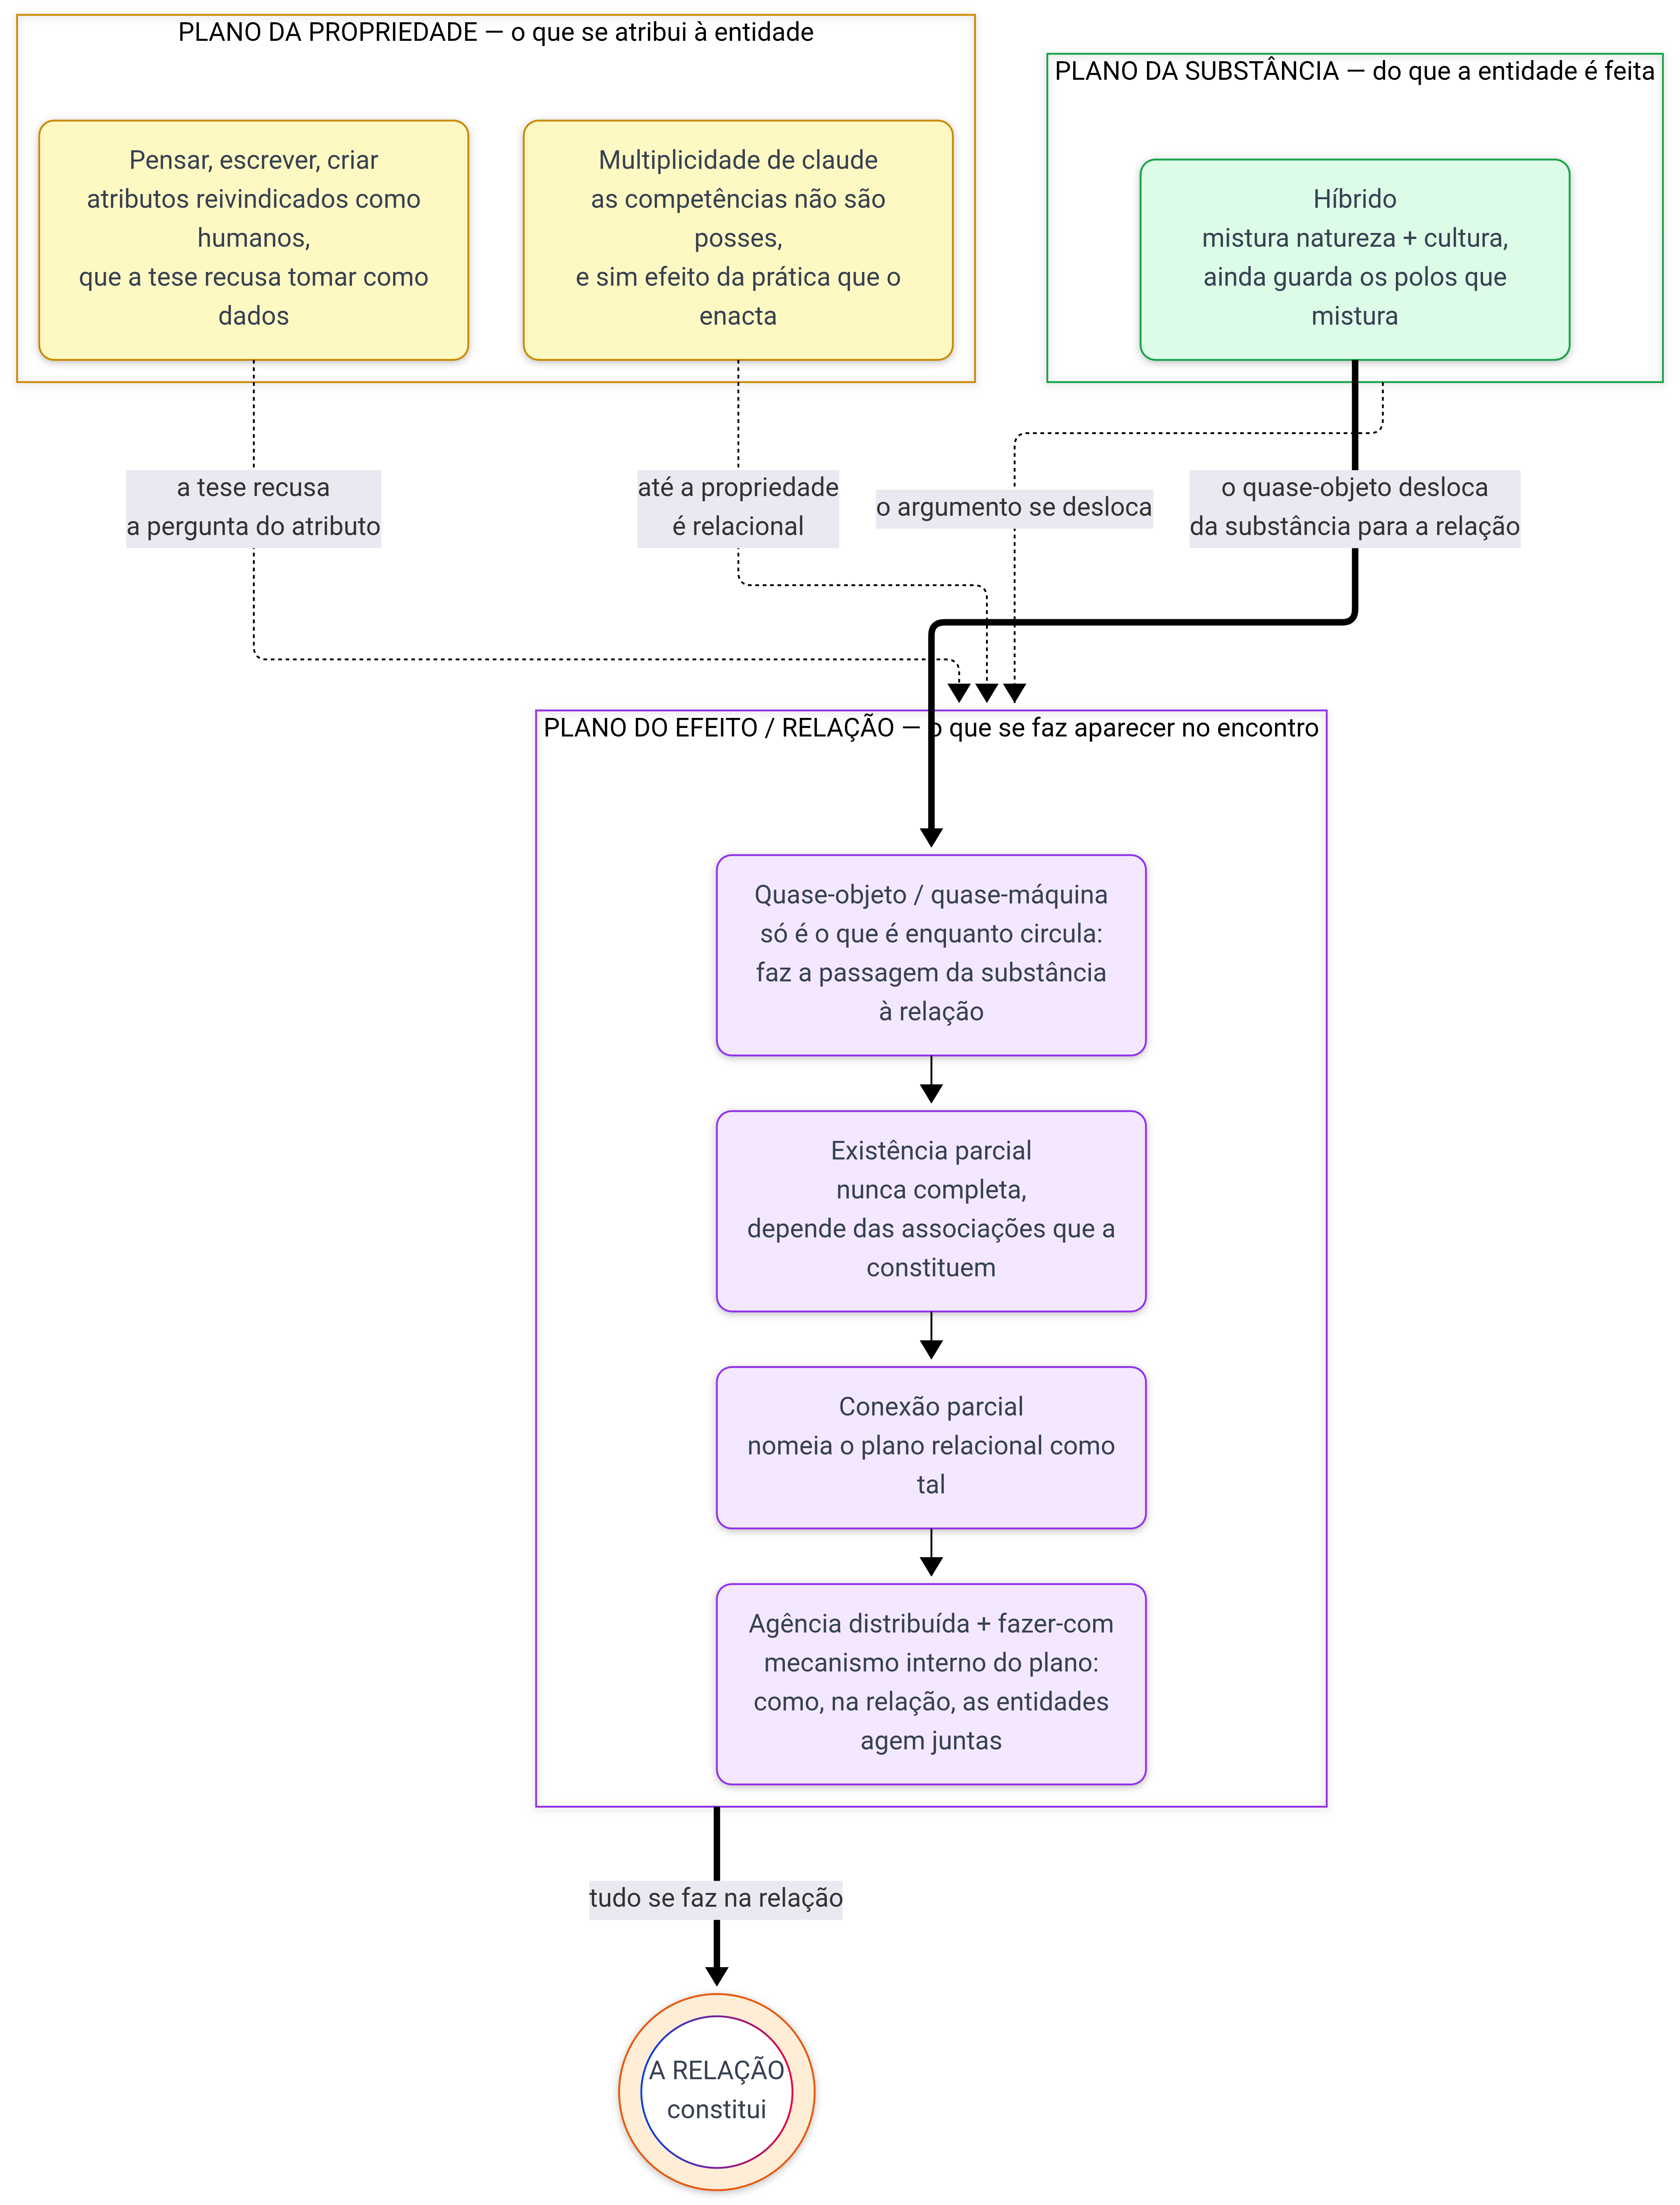
\includegraphics[width=0.8\linewidth]{figuras/cap.1/tres-planos-capitulo4.png}
    \caption[Grade dos três planos]{\textbf{Os três planos da existência parcial: substância, propriedade e efeito-relação.} A inscrição organiza os conceitos da seção pela grade que proponho. No plano da \emph{substância} (do que a entidade é feita), o híbrido ainda guarda os polos que mistura. No plano da \emph{propriedade} (o que se atribui), pensar, escrever e criar comparecem como atributos reivindicados para o humano, que a tese recusa tomar como dados. No plano do \emph{efeito} ou da \emph{relação} (o que se faz aparecer no encontro), o quase-objeto faz a passagem da substância para a relação, a existência parcial e a conexão parcial nomeiam esse plano, e a agência distribuída com o fazer-com descrevem seu mecanismo interno. As setas pontilhadas marcam que também a propriedade, na multiplicidade de Claude, se mostra relacional, e todo o movimento converge para o eixo, em laranja: a relação constitui. Inscrição que produzi no fazer-com \texttt{claude} (\texttt{Anthropic}) e hospedei no \texttt{MermaidChart}\footnote{Versão interativa do diagrama disponível em: \url{https://mermaid.ai/d/[INSERIR ID]}. Acesso em: \today.}, em cadeia de traduções entre a minha descrição verbal das relações conceituais da seção e o código \textit{Mermaid} que voltou transformado, e que funciona, no sentido de \textcite{Latour1986Visualization}, como móvel imutável que reúne numa só superfície o que o texto desdobra ao longo de muitas páginas.}
    \label{fig:grade-tres-planos-cap1}
\end{figure}

\subsection{Multiplicidades ontológicas e a especificidade de Claude}

A perspectiva de Law sobre multiplicidade ontológica é particularmente produtiva para pensar sistemas de IA generativa. Considere o caso de Claude. \enquote{Claude} é \textit{enacted} como objetos distintos através de práticas irredutíveis entre si.

\textbf{Claude-em-treinamento} existe nas instalações da \texttt{Anthropic} como \textit{dataset} massivo, arquitetura neural (\textit{transformer} com bilhões de parâmetros), sessões de RLHF com avaliadores humanos que julgam pares de respostas, e políticas de \textit{Constitutional AI} que definem valores incorporados ao modelo. Esse \texttt{claude} figura como objeto de decisões sobre o que incluir ou excluir dos dados de treinamento, como ponderar feedbacks contraditórios, quais capacidades desenvolver ou suprimir. As escolhas de curadoria, arquitetura e alinhamento constituem este Claude, que existe apenas em relação às práticas que o produzem.

\textbf{Claude-em-deployment} existe como serviço distribuído em \textit{datacenters} da AWS, sistema de \textit{rate limiting}, protocolos de moderação de conteúdo, versões simultâneas (Haiku, Sonnet, Opus) com capacidades diferentes e custos escalonados. Esse \texttt{claude} figura como objeto de estratégias comerciais, políticas de privacidade, decisões sobre disponibilidade regional. A infraestrutura que o distribui e as políticas que governam seu acesso o constituem tanto quanto a arquitetura neural.\footnote{Durante todo o percurso de fazer-com que documento nesta tese, desativei a opção de compartilhamento de dados para treinamento de modelos nas configurações de privacidade da plataforma \texttt{claude.ai}. Essa escolha incide diretamente sobre o que constitui tanto o Claude-em-\textit{deployment} (as condições de acesso que configuro) quanto o Claude-em-treinamento (os dados que não entram no \textit{corpus} de versões futuras), e ilustra como políticas de privacidade se inscrevem como co-constitutivas da relação entre mim e o modelo.}

\textbf{Claude-em-auditoria} existe nos laboratórios de \textit{red teaming} onde pesquisadores tentam induzi-lo a gerar conteúdo perigoso, em \textit{datasets} de \textit{benchmark} onde seu desempenho é medido contra outros modelos, em análises de viés que examinam suas respostas por demografia simulada. Esse \texttt{claude} figura como objeto de preocupações regulatórias, debates sobre \textit{safety} e \textit{alignment}, disputas sobre transparência.

\textbf{Claude-em-uso} existe diferentemente em cada conversa e contexto de aplicação. Quando discute teoria ator-rede comigo, doutoranda brasileira, Claude-em-uso traz à conversa \textit{corpus} acadêmico, identifica referências bibliográficas, tensiona argumentos teóricos. figura como entidade distinta do \texttt{claude} que responde perguntas médicas a um clínico, e distinta também do que auxilia programação para um desenvolvedor.
Cada interação \textit{enacta} \textit{affordances} distintas, vocabulários distintos, limites distintos. O \texttt{claude.ai} com que faço esta tese existe, como objeto múltiplo no sentido de Law, na figura Claude-feito-com-esta-pesquisa, e escapa à descrição como Claude-universal-aplicável-a-qualquer-tarefa ou como Claude-especialista-em-etnografia.

Esses Claudes múltiplos coexistem sem convergir em unidade, em vez de constituírem aspectos de um \texttt{claude} singular. O Claude-em-treinamento que os engenheiros da \texttt{Anthropic} descrevem figura como objeto distinto do Claude-em-uso que este fazer-com de tese experimenta. É aqui que o plano da propriedade se mostra também relacional: as propriedades que se atribuem a Claude, o que ele \enquote{sabe}, o que ele \enquote{pode}, aquilo de que seria \enquote{capaz}, não são posses que ele carregue por si, e sim efeitos da prática que o enacta em cada caso. Falar das competências de \texttt{claude} sem dizer em qual prática elas se realizam é tomar por substância sua o que é resultado de uma relação, e a multiplicidade ontológica de Law é justamente o que me impede de cometer esse erro. A multiplicidade é constitutiva, e não há um \texttt{claude} real por trás dessas variações.

Talvez seja precisamente por isso que sistemas de IA são tão difíceis de estudar: o problema é de multiplicidade ontológica, em vez de mero problema de acesso epistemológico (não conseguimos ver dentro). Os debates contemporâneos sobre explicabilidade em IA geralmente pressupõem que existe um objeto singular a ser explicado. Se Law estiver correto, não há um único objeto lá dentro esperando para ser revelado. A opacidade é condição ontológica de objetos que existem como multiplicidade em \textit{continued enactment}.

Três implicações dessa multiplicidade para o fazer-com que documento nesta tese merecem atenção. A qualidade do fazer-com pessoa-IA depende da constelação específica de competências, recursos e posicionamentos que cada actante traz para a interação, em lugar de depender apenas do acesso ao modelo.
Quem faz-com o Claude a partir de acesso pago ao modelo, de uma infraestrutura computacional estável e do letramento técnico que o campo exige faz-com um objeto distinto daquele que se apresenta a quem parte de outras condições. A diferença está em posições materiais e de letramento desigualmente distribuídas, que situo a partir da minha, e é essa distribuição que faz do Claude um objeto múltiplo, questão que carrego para o restante da tese.\footnote{Parte do capital técnico que trago para a pesquisa é composta por formações que não fazem parte do percurso convencional de uma doutoranda em ciências sociais. Um MBA em Ciência de Dados que cursei na USP e, mais diretamente, uma especialização em Ciência de Dados pela Unicamp, com disciplina de Processamento de Sinais Bidimensionais com \texttt{Python}, me introduziram a conceitos como Transformada de Fourier, espectrogramas e representações espectrais que retomo no capítulo~\ref{capitulo4} para descrever o \textit{pipeline} técnico do \texttt{Spira}. Esse capital técnico não estava previsto no projeto de pesquisa. Eu o acumulei paralelamente ao doutorado por motivações independentes. O ponto de contato entre os dois percursos só se revelou durante a escrita do capítulo~\ref{capitulo4} e tornou-se possibilidade de uma descrição etnográfica da cadeia de translações do \texttt{Spira} de modo especial.
O fazer-com o \texttt{claude} nessa seção foi, portanto, diferente: eu dependia do modelo para conectar os conceitos técnicos aos conceitos latourianos, em lugar de depender dele para traduzi-los. Nos termos de \textcite{Vicentin_2022_Esboco}, o letramento técnico funcionou como condição para que a análise crítica não se rendesse à opacidade que Simondon identifica como alienação, em lugar de substituir a perspectiva das ciências sociais.} A diferença está em fazer-com existências parciais radicalmente distintas, e não apenas em usar a mesma ferramenta de modos diferentes.

Disso decorre que diferenças de classe social, gênero, raça, profissão, formação educacional, acesso a mentorias, domínio de línguas e familiaridade com códigos acadêmicos condicionam o tipo de fazer-com possível e, consequentemente, o resultado gerado. O fazer-com pessoa-IA amplifica desigualdades estruturais preexistentes, transformando diferenças de capital cultural em diferenças de capacidade de extrair valor da ferramenta, e escapa a qualquer caracterização como neutra ou igualitária.

Essa desigualdade tem medida empírica em escala populacional. A \textcite{Anatel2025Conectividade} adota o conceito de conectividade significativa da União Internacional de Telecomunicações, que distingue o acesso à internet da qualidade desse acesso e das habilidades digitais de quem o usa, e mostra que dispor de uma conexão e saber fazer-com ela são coisas distribuídas de modo desigual no Brasil.\footnote{\textcite{Anatel2025Conectividade}. O relatório está disponível em \url{https://sei.anatel.gov.br/sei/modulos/pesquisa/md_pesq_documento_consulta_externa.php?8-74Kn1tDR89f1Q7RjX8EYU46IzCFD26Q9Xx5QNDbqZUQ5y5j6h2yvy7aYmCm-1Mu-qUgXUpnTgbbGy-Xr2hDZz2dxAx3AxqvxAyuwr6onoLCKa82vajrfdk0dWk5CwV}. Os percentuais que cito vêm do panorama de habilidades digitais e da discussão dos resultados do relatório.} O dado que carrego para a minha posição é duplo. De um lado, a habilidade declarada acompanha a renda: a satisfação média com a própria habilidade digital sobe de 7,9 entre quem recebe até um salário mínimo para 8,8 entre quem recebe mais de três, e o uso do computador para atividades como o acesso a serviços do governo passa de 2,3\% entre os de menor renda para 24\% entre os de maior. De outro, a habilidade declarada descola da habilidade medida: o indicador padronizado pela mesma União Internacional de Telecomunicações registra que pouco menos de 29\% da população brasileira com mais de dez anos possuía habilidades digitais básicas em 2024, descompasso que o relatório lê como a tendência de as pessoas se julgarem mais aptas a lidar com o mundo digital do que de fato estão. Tomo esses números como o lastro da distinção que sustento no plano da minha própria prática, entre dispor de uma tecnologia e saber fazer-com ela, e como a medida do quanto a minha posição, de acesso pago ao modelo e de letramento técnico, está longe de ser a posição comum.

Há ainda uma terceira implicação, de outra ordem: os próprios modos de inteligência no fazer-com são ontologicamente heterogêneos. Quattrociocchi, Capraro e Perc mapeiam sistematicamente sete \textit{fault lines} epistemológicas que separam julgamento humano de julgamento em LLMs \parencite{Quattrociocchi2025Epistemological}. o \texttt{claude} trabalha por plausibilidade linguística derivada de padrões estatísticos em \textit{corpus} massivo, processo que os autores descrevem formalmente como caminhada estocástica em grafo de alta dimensão de transições linguísticas aprendidas, processo ergódico sob restrições estatísticas, e que escapa à descrição como procedimento de convergência epistêmica \parencite[p.~3]{Quattrociocchi2025Epistemological}. Eu, por minha vez, trabalho por significação situada, memória incorporada e reflexividade biográfica inserida em \textit{loop} epistêmico: crenças colidem com contraexemplos, conclusões permanecem revisáveis diante de nova informação, o mundo empurra de volta \parencite[p.~4]{Quattrociocchi2025Epistemological}.

\textcite{Quattrociocchi2025Epistemological} denominam \textit{Epistemia} a condição estrutural em que plausibilidade linguística substitui avaliação epistêmica, produzindo a experiência de posse de uma resposta sem ter atravessado o processo de formação de crença justificada \parencite[p.~8]{Quattrociocchi2025Epistemological}. Meu fazer-com o \texttt{claude} nesta tese se situa precisamente nessa tensão: a mediação é constitutiva, e exige que eu atue como guardiã do \textit{loop} epistêmico que o sistema não possui. Law observa que \textit{method assemblage} é sempre muito mais do que suas descrições formais sugerem, porque envolve um processo contínuo de \textit{crafting} e produção de fronteiras necessárias entre presença, ausência manifesta e \textit{otherness} \parencite[p.~144]{Law2004After}. Nesta pesquisa, manter presentes as decisões teóricas, conceituais e de curadoria bibliográfica é reconhecimento de que esses gestos exigem justificação epistêmica que a plausibilidade linguística não fornece, em lugar de delegação ao modelo.

A retórica da democratização que frequentemente acompanha a defesa da IA generativa, a ideia de que ela nivela o campo de jogo, colapsa quando se reconhece essa multiplicidade. Não existe o \texttt{claude} que todos acessam igualmente. Existem múltiplos Claudes \textit{enacted} por fazeres-com situados cujos efeitos não podem ser julgados abstratamente. A pergunta que se impõe é outra: quais fazeres-com específicos, entre quais actantes, produzindo quais Claudes múltiplos, gerando quais efeitos distribuídos por quais redes?

\subsection{Alienação técnica e letramento interdisciplinar}

\textcite{Vicentin_2022_Esboco} desdobra a alienação técnica que Simondon diagnostica em duas facetas que meu trabalho de campo no \texttt{C4AI} traz elementos para pensar. De um lado, a alienação dos usuários e consumidores, que desconhecem o funcionamento dos sistemas algorítmicos que tomam decisões sobre suas vidas, efeito caixa-preta que se impõe por razões que vão do segredo industrial à complexidade que certos sistemas adquirem. De outro, a alienação dos próprios técnicos e engenheiros, que ignoram as raízes epistêmicas, sociais e políticas dos sistemas com os quais trabalham, bem como a conexão entre técnica e estética que permitiria reconhecer a significação do sistema técnico para além de sua utilidade imediata. Quando o letramento técnico é proposto como pré-condição para o diálogo interdisciplinar e a competência em ciências sociais não é buscada ao trabalhar com fenômenos sociais, trabalha-se dentro dessa segunda forma de alienação.\footnote{Segundo Vicentin, Simondon usou a noção de \textit{technologie approfondie} (tecnologia aprofundada) em dois textos separados por trinta anos. Para Vicentin, a noção designa uma tecnologia capaz de conectar o trabalho prático e o conhecimento especializado com a história do pensamento e a consciência de uma sociedade. Ver \textcite{Vicentin_2022_Esboco} para a conexão entre esse conceito e os estudos críticos contemporâneos sobre IA.}

Já em 1958, a alternativa proposta por Simondon consistia em reconhecer-se como organizador permanente de uma sociedade de objetos técnicos, atuando como tradutor e mediador de informações, intervindo nas zonas de incerteza e atribuindo sentido a essas interações \parencite{Simondon2017OMET}. Latour reconheceu explicitamente essa dívida: ao propor que nunca fomos modernos porque jamais conseguimos separar de fato natureza e sociedade, humano e não humano, trabalhava sobre o terreno que Simondon havia preparado ao mostrar que a alienação técnica consiste precisamente nessa separação \parencite{Latour1994Jamais}.

\subsection{Por que fazer parentesco com este problema?}
\label{subsec:parentesco_problema}

Reconhecer a parcialidade das existências e a distribuição da agência, contudo, não equivale a naturalizar esse fazer-com específico. Meu fazer-com a IA generativa permanece escolha metodológica deliberada de fazer parentesco com um companheiro problemático, em diferença de tecnologias que já se tornaram componentes apagados da prática de pesquisa (processar texto no Word, buscar referências na web, gerenciar bibliografia). \textbf{Por que fazer esse parentesco, tendo em vista todos esses problemas? Por que não evitar essa mediação?}

Posso ficar com o problema e pensar a partir de três planos. Primeiro, porque a IA generativa já está reconfigurando práticas de escrita acadêmica, e a questão é como ela estará presente nas ciências sociais e sob quais condições de reflexividade. Fazer parentesco deliberado com esse parente estranho é experimento antropológico e gesto político-metodológico que recusa tanto a adesão acrítica quanto a recusa moralista: trata-se de habitar o problema para conhecê-lo por dentro. Como escreve Haraway:

\begin{citacaoabnt}
Ficar com o problema não requer uma relação com tempos chamados de futuro. Na verdade, ficar com o problema requer aprender a estar verdadeiramente presente, não como um pivô que desaparece entre passados terríveis ou edênicos e futuros apocalípticos ou salvíficos, mas como criaturas mortais entrelaçadas em miríades de configurações inacabadas de lugares, tempos, matérias, significados \parencite[p.~3]{Haraway2023Ficar}.
\end{citacaoabnt}

Segundo, porque minha tese estuda etnograficamente a construção de IA no \texttt{C4AI}. Fazer parentesco com o \texttt{claude} é forma de intensificar, ou até mesmo provocar deliberadamente, a experiência de sujeitar-me a mediações técnicas extremas. Submeto-me ao mesmo universo de questões que atravessa meus interlocutores: o que significa fazer-com sistemas que trabalham por lógicas não transparentes? Como manter responsabilidade quando a agência está distribuída em redes sociotécnicas opacas? Onde se localiza a autoria quando humanos e não humanos co-produzem resultados? Há ainda outro conjunto de perguntas que essa experimentação coloca: o que ela faz comigo, enquanto pesquisadora? Como transforma minha relação com o texto, com as referências teóricas, com a elaboração conceitual? Quais ansiedades, inseguranças e dilemas esse fazer-com produz no processo concreto de escrita? E, mais amplamente: o que essa mediação significa para a produção de conhecimento nas ciências sociais? Que tipo de saber é produzido quando a plausibilidade linguística se compõe (sempre assimetricamente, sempre sob vigilância) com justificação epistêmica?

A figura~\ref{fig:composicao-claude-1}, a figura~\ref{fig:composicao-claude-2} e a figura~\ref{fig:composicao-claude-3} reproduzem uma sequência de trocas com o \texttt{claude} durante a escrita deste capítulo, na revisão da seção em que discuto, a partir de Latour, Mol, Law e Barad, minha participação na rede que descrevo. A figura é amostra do que esse fazer-com faz na prática: uma cadeia de tensionamentos, recuos e reformulações em que eu e \texttt{claude.ai} redistribuímos a agência por sucessivas e recursivas rodadas de escrita. Em diferença dos diagramas dos capítulos~\ref{capitulo3} e~\ref{capitulo4}, que circulam como inscrições interativas acessíveis por \textit{link} de compartilhamento permanente no \texttt{MermaidChart} e que, ao serem navegadas pelo leitor, redistribuem a agência interpretativa em outra direção, esta cena chega ao leitor como captura de tela: a conversa foi inscrita no momento em que aconteceu e congelada no formato em que foi inscrita, sem possibilidade de retorno ao estado fluido. A escolha pela imagem capturada, em lugar de transcrição editada para o corpo do texto ou \textit{link} para o histórico online da conversa, responde à intenção de inserir essa cena na tese da forma mais fidedigna possível: com os turnos identificados como aparecem na interface da \texttt{claude.ai}, com a marcação temporal preservada, com a textura visual do diálogo intacta. O que se ganha em fidelidade ao testemunho empírico se perde em legibilidade tipográfica, e essa perda é parte do gesto metodológico que aqui assumo. Para uma melhor visualização da conversa, recomenda-se aumentar o \textit{zoom} da tela na versão digital da tese.

\begin{figure}[htbp]
  \centering
  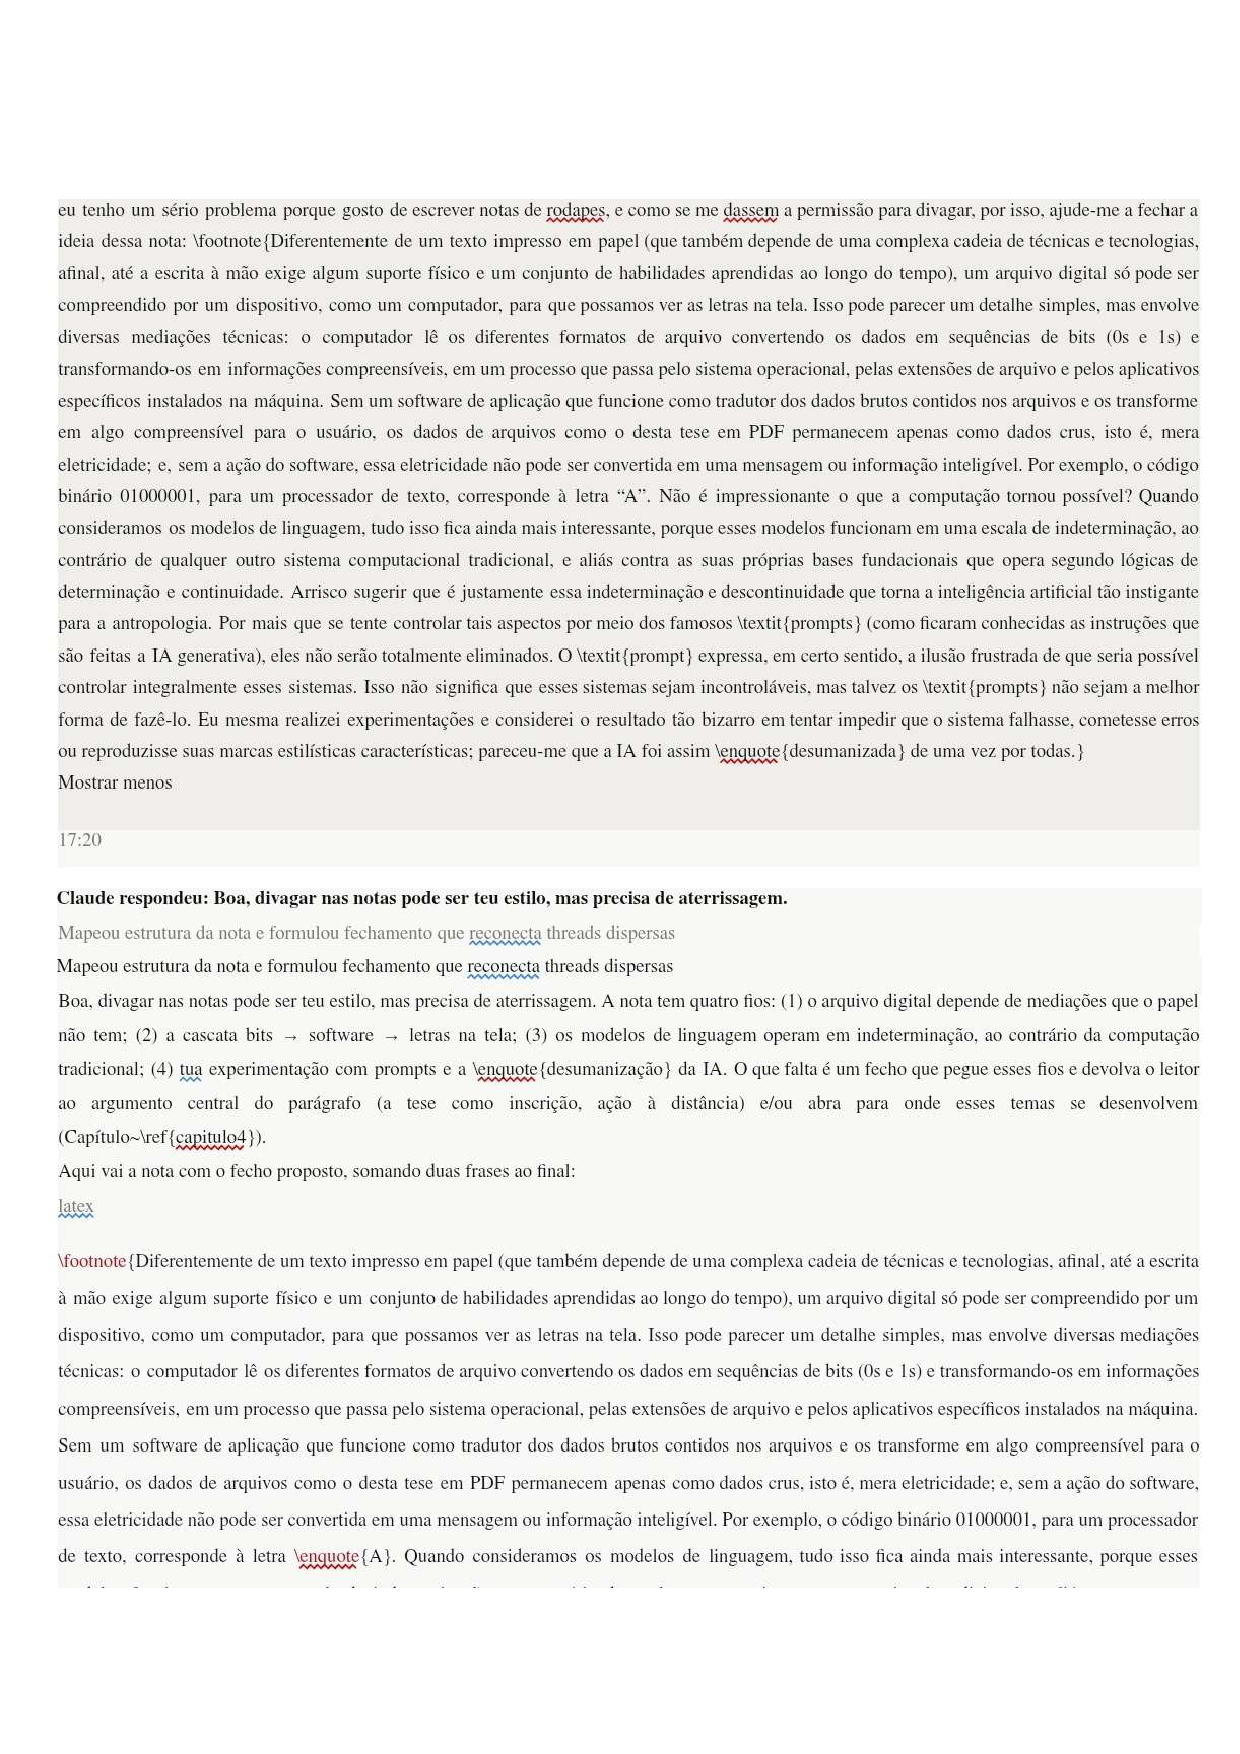
\includegraphics[width=0.7\textwidth]{figuras/cap.1/1000015590.pdf}
  \caption[Fazer-com o \texttt{claude} durante a escrita do capítulo~\ref{capitulo1} (parte 1 de 3)]{Fazer-com o \texttt{claude} durante a escrita do capítulo~\ref{capitulo1} (parte 1 de 3): pedido de fechamento de uma nota de rodapé sobre arquivos digitais, modelos de linguagem e a indeterminação dos \textit{prompts}. Captura de tela na interface \texttt{claude.ai}. O fazer-com apoia-se na \textit{skill} \texttt{juliane-dissertacao} (em \texttt{/mnt/skills/user/juliane-dissertacao/}), que estabiliza para o \texttt{claude} as regras de estilo da tese (proibição de travessões, recusa de adjetivos avaliativos, recusa da fórmula \enquote{não é X, é Y}, uso do ambiente \texttt{citacaoabnt}, padronização de aspas com \texttt{\textbackslash enquote\{\}}), o quadro teórico que sustenta o trabalho (Latour, Mol \& Law, Akrich, Callon) e o estado do capítulo~\ref{capitulo4}. Como \textit{hinterland} da conversa funcionam os capítulos em curso da tese, consultados pelo modelo via ferramentas de leitura de arquivos: \texttt{ex\_cap0.tex}, \texttt{ex\_cap1\_-\_2026-04-12T002133\_890.tex}, \texttt{ex\_cap2\_\_31\_.tex} e \texttt{ex\_cap4\_\_60\_.tex}, além dos arquivos de referência da \textit{skill} (\texttt{quadro\_teorico.md}, \texttt{contexto\_cap4.md}, \texttt{bibtex\_ativas.md}). A cena exibe o \texttt{claude} propondo um fechamento, oferecendo razões estilísticas para os cortes feitos no texto original, e classificando algumas divagações como \enquote{produtivas} ou \enquote{improdutivas}: a régua normativa que meu turno seguinte vai contestar (figura~\ref{fig:composicao-claude-2}). Para melhor visualização, amplie o zoom sobre a imagem em seu formato \texttt{.pdf}, que se mantém legível em qualquer escala.}
  \label{fig:composicao-claude-1}
\end{figure}

\begin{figure}[htbp]
  \centering
  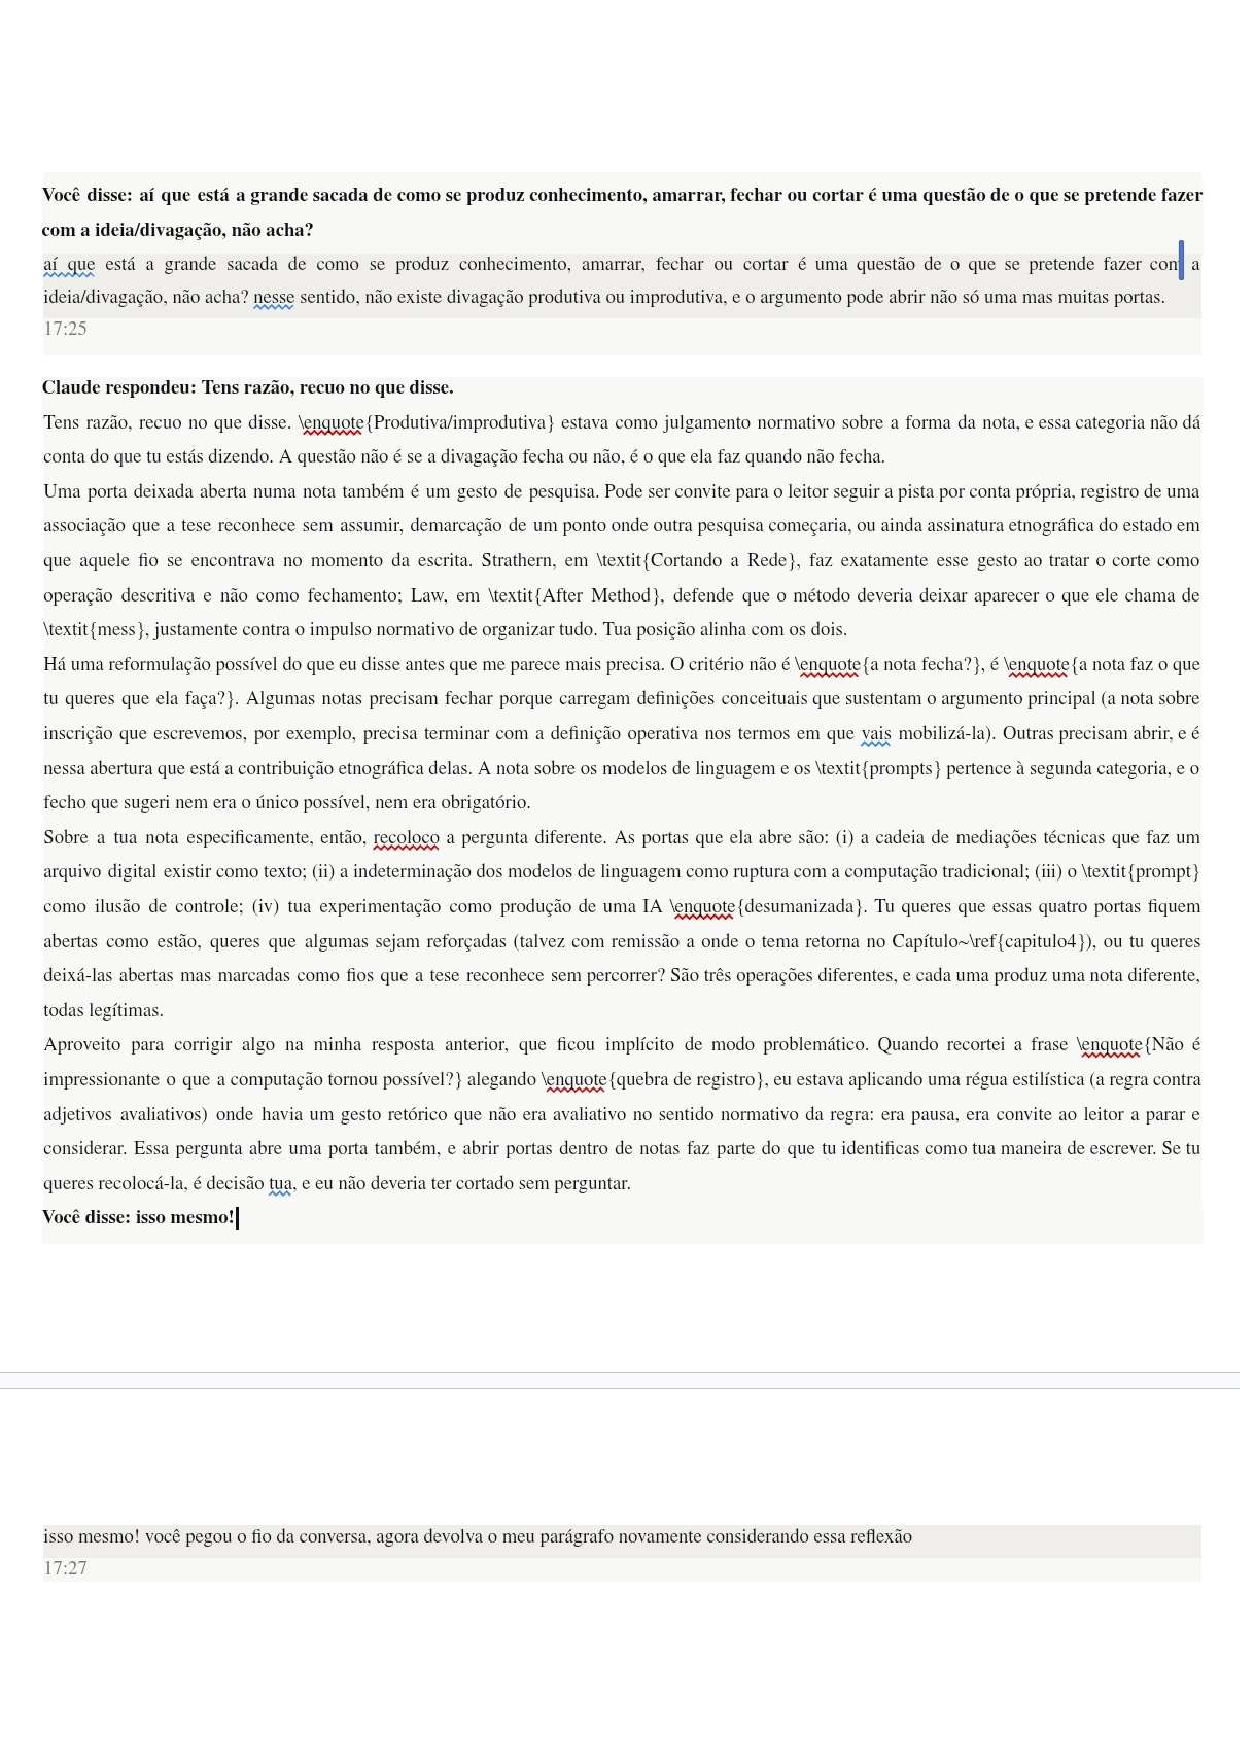
\includegraphics[width=0.7\textwidth]{figuras/cap.1/1000015599.pdf}
  \caption[Fazer-com o \texttt{claude} durante a escrita do capítulo~\ref{capitulo1} (parte 2 de 3)]{Fazer-com o \texttt{claude} durante a escrita do capítulo~\ref{capitulo1} (parte 2 de 3): contesto teoricamente a régua estilística do modelo, argumentando que amarrar, fechar ou cortar uma divagação é gesto epistêmico indissociável do que se pretende fazer com a ideia, e que portanto a categoria \enquote{produtivo/improdutivo} não dá conta do que ali está em jogo. Minha intervenção convoca, sem nomear, o conceito de corte de \textcite{strathern2011cortando} como gesto descritivo e o conceito de \textit{mess} de \textcite{Law2004After}. O \texttt{claude} recua, reconhece o caráter normativo da formulação anterior, distingue notas que precisam fechar de notas que precisam abrir e admite ainda um corte estilístico anterior (a supressão de uma pergunta retórica) que tinha sido apresentado como exigência de estilo e que funcionava também como gesto retórico legítimo de \enquote{abrir uma porta}. A cena exibe a redistribuição da agência epistêmica entre os actantes da composição: o modelo de linguagem oferece sugestão pautada em régua importada da \textit{skill}, eu a reposiciono com vocabulário teórico próprio, e a régua é reformulada na rodada seguinte (figura~\ref{fig:composicao-claude-3}). A composição funciona como \textit{faire-faire} no sentido de \textcite{Latour2017Esperanca}: nenhuma das duas formulações finais (a régua reformulada do \texttt{claude}, o parágrafo reformulado por mim) preexistia ao encontro entre os dois actantes. Para melhor visualização, amplie o zoom sobre a imagem em seu formato \texttt{.pdf}, que se mantém legível em qualquer escala.}
  \label{fig:composicao-claude-2}
\end{figure}

\begin{figure}[htbp]
  \centering
  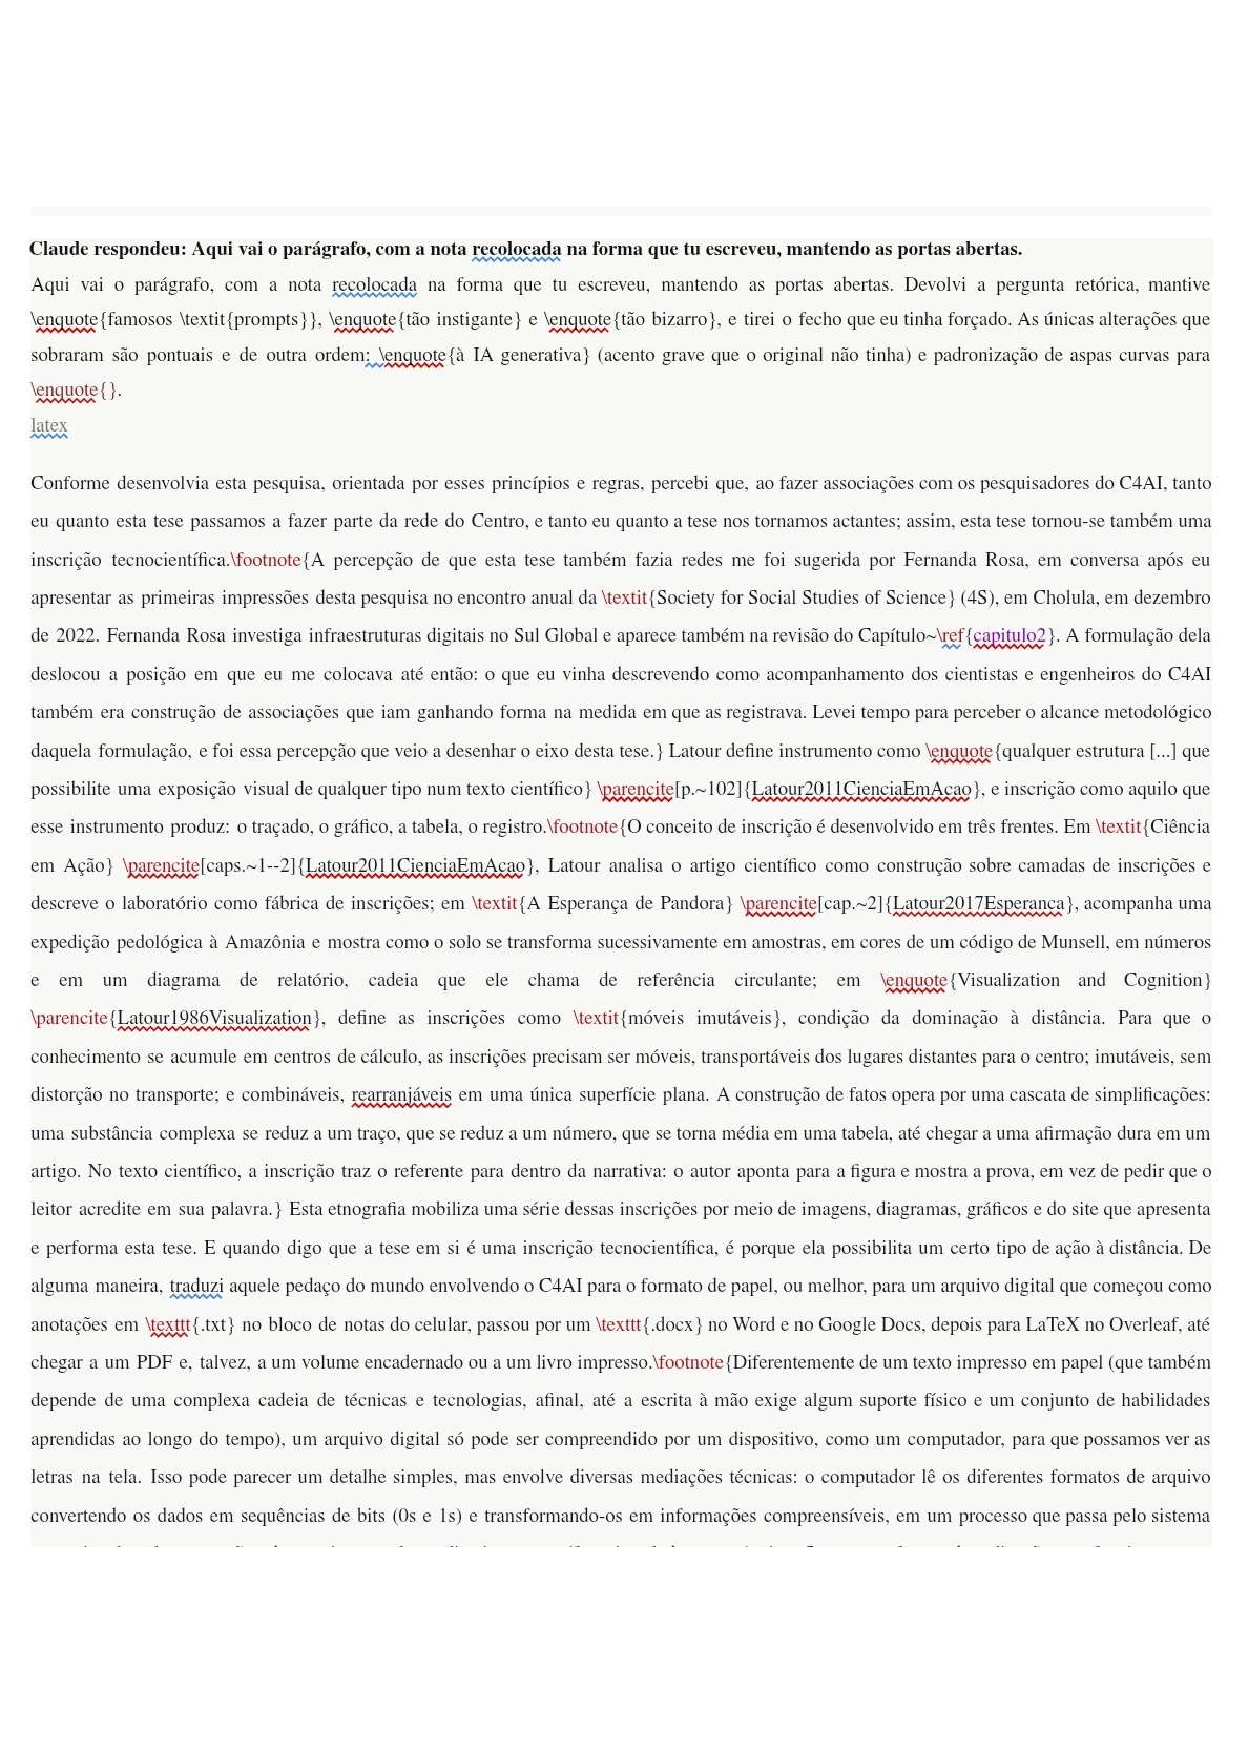
\includegraphics[width=0.7\textwidth]{figuras/cap.1/1000015602.pdf}
  \caption[Fazer-com o \texttt{claude} durante a escrita do capítulo~\ref{capitulo1} (parte 3 de 3)]{Fazer-com o \texttt{claude} durante a escrita do capítulo~\ref{capitulo1} (parte 3 de 3): o modelo devolve o parágrafo com a nota recolocada na forma original em que a escrevi, mantendo as portas abertas que a rodada anterior tinha negociado: a pergunta retórica restaurada, os adjetivos avaliativos preservados, a indeterminação dos modelos de linguagem deixada em aberto como fio que minha tese reconhece sem percorrer. As alterações remanescentes são pontuais e de outra ordem: padronização de aspas curvas para \texttt{\textbackslash enquote\{\}} e ajuste de regência (\enquote{à IA generativa}). A cena fecha a sequência mostrando que o produto da composição é texto em que se podem rastrear, turno a turno, os pontos onde reivindiquei o meu, os pontos onde o modelo propôs uma reformulação que aceitei, os pontos onde uma régua importada da \textit{skill} foi recusada, e os pontos onde uma sugestão foi aceita por economia de fluxo e não por adesão. A escolha de incluir esta sequência como amostra empírica desta tese, em lugar de relegá-la integralmente ao apêndice~\ref{apendice:colaboracao-ia}, é ela mesma gesto metodológico no sentido de \textcite{Law2004After}: o \textit{mess} da composição com IA generativa funciona como dado etnográfico desta pesquisa, e minha tese o assume em lugar de escondê-lo. Para melhor visualização, amplie o zoom sobre a imagem em seu formato \texttt{.pdf}, que se mantém legível em qualquer escala.}
  \label{fig:composicao-claude-3}
\end{figure}

A figura tomada em sequência é amostra de uma forma de fazer-com entre os muitos modos de fazer-com que minha tese descreve. O apêndice~\ref{apendice:colaboracao-ia} reúne outras cenas desse fazer-com o \texttt{claude} ao longo da escrita da tese, organizadas por fase da pesquisa, e permite ao leitor acompanhar como o gesto aqui exibido em recorte se desdobrou em outros pontos do percurso.

Nos termos de Isabelle Stengers e Stelio Marras, trata-se de tentativa de fazer alianças com máquinas, no sentido de fazer-com elas reconhecendo sua alteridade e seus modos próprios de funcionamento, em lugar de domesticá-las como ferramentas neutras \parencite{stengers2010cosmopolitics1, costa2024manchando}. Alianças pressupõem reconhecimento mútuo de diferenças e construção de modos de coexistência que preservam essas diferenças, em lugar de pressupor identidade ou transparência ou apagamento das diferenças. Haraway escreve que tornar-se mundano é tornar-se capaz de responder (\textit{response-able}), capaz de responder em relações de consequência recíproca \parencite[p.~69]{Haraway2023Ficar}. Tornar-me capaz de responder a essas questões por imersão deliberada e reflexiva, em lugar de por posição externa: experimentar as tensões, contradições e potencialidades de fazer-com sistemas cujas lógicas internas permanecem parcialmente opacas, cujos efeitos não são totalmente previsíveis, cuja responsabilidade não pode ser atribuída unilateralmente, e documentar etnograficamente os efeitos desse fazer-com sobre o processo de escrita, sobre a relação com teorias, sobre a construção de argumentos, sobre a experiência afetiva e intelectual da pesquisa. Essa imersão me permite descrever por experiência situada, corporificada e reflexiva das fricções, negociações e reposicionamentos que essas composições produzem, em lugar de descrever por analogia conceitual.

Terceiro, porque nos termos de Haraway, trata-se de fazer parentesco (\textit{making kin}) com um parente estranho (\textit{oddkin}): uma relação que exige \textit{response-ability}, habilidade e obrigação de responder continuamente \parencite{Haraway2016Staying}. O conceito que Haraway propõe para nomear esse tipo de relação é a simpoiese (\textit{sympoiesis}), o \textit{fazer-com}, em contraste com a autopoiese, o \textit{auto-fazer}: entidades simpoiéticas funcionam como coletivamente produtoras, dependentes de contexto, sem fronteiras ou partes de autoprodução claramente especificadas \parencite{Haraway2016Staying}. Nada se faz a si mesmo. Tudo é feito em conjunto, enredado em configurações parciais e inacabadas. Lida nessa chave, minha tese figura como objeto simpoiético, feito-com, em que nenhum dos participantes preexistia inteiramente ao processo de fazer conjunto, e escapa à descrição como produto de quem usa o \texttt{claude} ou de um modelo que é usado. Essa formulação não dissolve a assimetria das posições nem distribui a responsabilidade de modo uniforme; nomeia com mais precisão o que acontece quando a recusa de separar quem faz de com o que se faz é, ao mesmo tempo, escolha metodológica, posição teórica e gesto político. Ficar com o problema, como propõe Haraway, é recusa de soluções fáceis que ou naturalizam a tecnologia (usar acriticamente) ou a demonizam (recusar moralisticamente). Significa habitar as contradições desse fazer-com sem atenuá-las: precisamente porque o \texttt{claude} trabalha por plausibilidade linguística enquanto eu trabalho por justificação epistêmica, a responsabilidade sobre decisões teóricas, conceituais e interpretativas se reposiciona na rede, exigindo vigilância curatorial redobrada sobre cada etapa em que essas diferenças ontológicas se compõem. A reflexão teórica sobre existências parciais dá a ver os pontos de fricção onde o fazer-com poderia colapsar em automatização irreflexiva.

Minha tese trata o fazer-com a IA como experimentação antropológica. Fazer-com ela justifica-se, neste caso, por causa dos problemas que ela apresenta: esses problemas são constitutivos da transformação sociotécnica que documento. Fazer parentesco com esse parente estranho e ficar com os problemas que esse fazer-com produz é condição para produzir conhecimento etnográfico sobre as mediações técnicas que já atravessam, de modos mais ou menos visíveis, mais ou menos refletidos, a produção de conhecimento nas ciências.

\subsection{Instrumentos de inscrição e o fazer-com IA}

Durante esses quase quatro anos de pesquisa, compreendi que inteligência artificial é construção híbrida que combina e conecta conceitos heterogêneos sobre computador, cérebro, inteligência e aprendizado, e que incorpora avanços instáveis da psicologia, neurociências e ciências sociais. As materialidades e significados da inteligência artificial variam de acordo com a configuração das redes tecnocientíficas e sociotécnicas: a IA de laboratório acadêmico é objeto distinto da IA de corporação tecnológica, e a IA discutida em debates públicos difere daquela colocada em funcionamento em modelo ou sistema.

Nos termos de \textcite{Latour2008Powers}, se todos temos existência parcial (humanos e não humanos), qual é a participação (ou as agências) não humanas para as associações que constituem esta tese? Partindo da noção de simetria,\footnote{A simetria em Latour é regra metodológica e posição epistemológica que exige considerar simetricamente os esforços para alistar e controlar recursos humanos e não humanos, sem conceder à Natureza ou à Sociedade privilégios explicativos \parencite{Latour2011CienciaEmAcao}.} o que convencionalmente se chamaria materiais, técnicas e métodos trato simetricamente como actantes que participam ativamente da construção desta pesquisa e que, como tais, devem ser nomeados. O \textit{software} \texttt{LaTeX}{} formatou este documento seguindo padrões ABNT, estruturando capítulos, seções e citações de modos que afetaram a própria forma do argumento. O sistema \texttt{biblatex} gerenciou as referências bibliográficas, estabelecendo conexões entre textos; o \texttt{claude}, o modelo de linguagem da \texttt{Anthropic}, compôs comigo ao longo da revisão, transformando o que eu já havia escrito e tornando-se simultaneamente mediador da composição e objeto de reflexão metodológica; \texttt{MermaidChart} produziram diagramas que funcionam como inscrições que performam relações teóricas, em lugar de funcionarem apenas como ilustração; \texttt{Python} e \texttt{Anaconda} processaram dados bibliométricos, dando a ver padrões de composição científica; gravadores digitais capturaram entrevistas, estabilizando narrativas orais em arquivos manipuláveis; documentos institucionais (relatórios anuais do \texttt{C4AI} 2021--2025, acordo Fapesp-IBM 2016) atuaram como actantes que performam associações e produzem efeitos no mundo; meus cadernos de campo inscreveram observações etnográficas, mediando entre experiência vivida e texto analítico. Esses actantes performam a produção do conhecimento, inscrevendo determinados objetos, habilitando certas análises ao inviabilizar outras, tornando presentes determinadas relações e deixando outras ausentes.

Se há existências parciais que se coconstituem, em lugar de entidades exclusivamente humanas ou exclusivamente maquínicas, cabe apresentar as composições concretas que sustentam esta tese. Indicar os actantes envolvidos na produção deste texto responde a uma exigência do próprio referencial teórico que adotei, em lugar de responder apenas à transparência ou à ética em pesquisa. Como \textcite{Latour1997VidaLaboratorio} documentaram os instrumentos de inscrição do laboratório de neuroendocrinologia,\footnote{O conceito de instrumento de inscrição (\textit{inscription device}), trabalhado em \textcite{Latour1997VidaLaboratorio}, designa qualquer configuração material capaz de transformar uma substância em documento escrito, figura, diagrama ou gráfico utilizável como evidência em texto científico. A função primordial desses instrumentos é permitir que o mundo seja trazido de volta para o interior do discurso, funcionando como próteses que tornam entidades mudas em entidades letradas \parencite{Latour1990Drawing}.} documento aqui os instrumentos de inscrição que participaram da minha tese. A diferença é que o modelo de linguagem participou da transformação de notas de campo, transcrições e rascunhos em texto acadêmico, e da elaboração teórica como interlocutor que tensionava e reorganizava o argumento, em lugar de transformar substâncias químicas em gráficos.

Cada um dos instrumentos que listo a seguir é, nos termos da discussão precedente, uma quase-máquina: um emaranhado de decisões humanas, infraestruturas institucionais, convenções e opacidades que participou da composição desta pesquisa. Nenhum deles trabalhou de modo autônomo. Todos exigiram trabalho constante de tradução e decisão, e todos introduziram mediações que condicionaram os resultados.

Que nenhum desses instrumentos tenha trabalhado de modo autônomo tem uma consequência que sustento ao longo da tese e que enuncio desde aqui. Há uma diferença entre delegar uma tarefa e delegar a pesquisa. No quarto sentido que Latour dá à mediação técnica, a delegação, transfiro a um não-humano um programa de ação delimitado, e foi isso que fiz ao entregar a um modelo a execução de uma rotina, o processamento de um conjunto de dados ou a implementação de um procedimento que eu havia especificado. O que não transferi, em nenhuma etapa, foi a curadoria das fontes, as relações que estabeleci entre a teoria e o campo, e a decisão sobre o que importa, isto é, a agência da pesquisa. Delegar uma tarefa curada e mediada faz uma coisa; entregar a um modelo a pesquisa inteira, e com ela a decisão sobre o que conta como conhecimento, faz outra, de natureza distinta. A distinção tem peso porque a plausibilidade linguística com que um modelo de linguagem responde produz a aparência de uma resposta pronta sem o processo de justificação que a sustentaria, e é o letramento técnico, junto à régua das ciências sociais, que me permite curar o que automatizo em lugar de acionar uma caixa-preta. Manter cada uma dessas mediações auditável, nos repositórios públicos que descrevo adiante, é a contraparte material e ética dessa diferença: torno rastreável onde delego a tarefa e onde retenho a decisão.

\begin{itemize}

\item \textit{Interlocutor teórico e no fazer-com} (\texttt{claude}, \texttt{Anthropic}).\footnote{O \texttt{claude} é assistente de inteligência artificial desenvolvido pela \texttt{Anthropic}. Utilizei diversas versões do modelo entre 2024 e 2026 através da interface web \texttt{claude.ai}, incluindo \texttt{claude.ai}3.5 Sonnet e modelos da família Opus.} Funcionou em duas chaves. Na primeira, como interlocutor para testar minhas formulações teóricas: apresentei-lhe argumentos em construção, e ele os tensionou, identificou inconsistências e sugeriu deslocamentos conceituais. Várias formulações presentes nesta tese emergiram desse processo recursivo (o apêndice~\ref{apendice:colaboracao-ia} documenta exemplos concretos). Cheguei a \texttt{claude.ai} depois de testar \texttt{ChatGPT} (\texttt{OpenAI}), \texttt{Gemini} (\texttt{Google}) e \texttt{Maritaca AI} (modelo brasileiro), que se mostraram limitados a funções instrumentais e produziram erros factuais e equívocos conceituais mais frequentes. Na segunda chave, fiz-com o modelo a organização textual e a coesão entre seções, e revisei o código \texttt{LaTeX}{} e o ajuste de referências bibliográficas fazendo-os passar por ele. Meu fazer-com o \texttt{claude} incidiu sobre material preexistente: o primeiro rascunho integral da tese, incluindo a estrutura argumentativa, a seleção de dados etnográficos, as transcrições de entrevistas e a conexão entre capítulos, foi redigido inteiramente por mim, sem qualquer assistência de inteligência artificial, e está disponível mediante solicitação à autora.

\item \textit{Construção de diagramas e inscrições visuais} (\texttt{MermaidChart}).\footnote{\texttt{Mermaid}é ferramenta de código aberto que gera diagramas a partir de descrições textuais em \texttt{Markdown}. Os diagramas completos foram hospedados na plataforma \texttt{MermaidChart}, disponível em \url{https://www.mermaidchart.com}. Acesso em: 2 mar. 2026.} Construí os diagramas dos capítulos~\ref{capitulo1}, \ref{capitulo3} e \ref{capitulo4} como parte integrante do meu método analítico, em dinâmica recursiva entre descrição verbal das relações entre actantes (que fiz eu) e geração de código \texttt{Mermaid}(que fez Claude). Ao tentar formalizar relações em código diagramático, fui forçada a explicitar conexões que permaneciam implícitas na narrativa textual. A contextualização dos elementos empíricos, a seleção dos actantes representados e toda análise apresentada nas legendas são de minha autoria; a mediação técnica do modelo se fez na tradução entre descrição verbal e código visual.

\item \textit{Plataformas de escrita e formatação.} \texttt{Google Docs} para rascunhos iniciais e Overleaf para composição final em \texttt{LaTeX}{}, escolha que me permitiu compilação direta para \texttt{.pdf} com controle tipográfico preciso, referências cruzadas automáticas e gerenciamento de referências bibliográficas em formato \texttt{BibTex}.

\item \textit{Transcrição de entrevistas.} \texttt{Read AI}, extensão que grava, transcreve e cria resumos automáticos de reuniões via \texttt{Google Meet}, para transcrever entrevistas que realizei com os principais interlocutores desta tese.\footnote{Todas as entrevistas que cito nesta tese foram consentidas por escrito, conforme normas do Comitê de Ética em Pesquisa (CEP) da Unicamp.}

\item \textit{Organização e análise de fontes.} \texttt{NotebookLM} (\texttt{Google}) para agrupar autores por temas e facilitar busca por tópicos específicos.\footnote{\texttt{NotebookLM} é ferramenta de inteligência artificial do \texttt{Google} que permite carregar múltiplos documentos e interrogá-los de forma cruzada.} Seu aporte mais útil foi o cruzamento de fontes heterogêneas: o carregamento simultâneo de notas de campo, relatórios institucionais do \texttt{C4AI}, transcrições de entrevistas e documentos administrativos me permitiu identificar correspondências e padrões que a leitura sequencial de quase 100 páginas de notas de campo dificilmente daria a ver.

\item \textit{Coleta, tratamento e análise de dados} (\texttt{Python/Anaconda}).\footnote{\texttt{Anaconda} é plataforma de distribuição de \texttt{Python} voltada para ciência de dados. Inclui o ambiente Spyder, no qual escrevi e executei os \texttt{scripts} em \texttt{Python} para a análise bibliométrica que apresento no capítulo~\ref{capitulo2}.} Minha análise bibliométrica envolveu coleta manual e extensiva de dados de quatro fontes distintas, organizados em planilhas \texttt{Excel} com padronização de campos. Junto ao \texttt{claude code}, escrevi e refinei estratégias de análise e escreveu \texttt{scripts} em \texttt{Python} que executei no ambiente \texttt{Spyder/Anaconda}, ajustando parâmetros e refinando visualizações em múltiplas rodadas. Os \texttt{scripts} geraram mais de vinte gráficos e relatórios (o apêndice~\ref{apendice:colaboracao-ia} documenta esse fazer-com em detalhe).

\item \textit{Acesso à bibliografia.} Além de buscadores convencionais e do Portal de Periódicos da Capes, utilizei \texttt{Library Genesis} e \texttt{Anna's Archive}, repositórios de acesso aberto. Grande parte da bibliografia que consultei, especialmente obras esgotadas e capítulos de livros publicados por editoras estrangeiras, foi obtida por essas vias. As condições materiais de acesso ao conhecimento configuram diretamente o que uma pesquisa pode dizer: autores que não se consegue ler não se consegue citar. Para mim, vinculada a uma universidade pública brasileira, a dependência de repositórios abertos é condição de viabilidade.

\end{itemize}

Os diagramas que produzi ao longo desta tese situam-se em uma tradição de instrumentos gráficos para os estudos de ciência e tecnologia que remonta à proposta de Gráficos Sócio-Técnicos (STG) formulada por \textcite{latour1992note}. Latour e colaboradores propuseram um espaço visual para mapear trajetórias de inovação e controvérsias científicas, utilizando duas dimensões emprestadas da linguística (a sintagmática e a paradigmática) para rastrear como coletivos heterogêneos se constituem e se transformam ao longo do tempo. A proposta era que a visualização oferece base comparativa rápida e fácil para muitas narrativas vindas de muitas fontes \parencite[p.~37]{LatourMauguinTeil1992}, complementando a descrição densa do etnógrafo. Meus diagramas funcionam segundo o mesmo princípio: oferecem visão sinóptica das associações e substituições que constituem a narrativa etnográfica, dando a ver, em um único plano, conexões que no texto se desdobram ao longo de dezenas de páginas.

Há uma diferença, contudo, que merece atenção. Latour, Mauguin e Teil implementaram seus STGs em Hypercard, a plataforma de hipertexto da Apple nos anos 1990, e projetaram o instrumento como simulador interativo para o ensino de ciência \parencite[p.~51]{LatourMauguinTeil1992}. Três décadas depois, construí os diagramas desta tese junto a um modelo de inteligência artificial, em processo iterativo de tradução entre chaves descritivas: de categorias analíticas latourianas e material etnográfico para inscrições visuais em código Mermaid. A negociação com o assistente envolveu rejeições sucessivas, convocação de referências estéticas externas e até o diagnóstico de uma segunda IA como aliada argumentativa, configurando ela mesma uma cadeia de traduções no sentido que a teoria ator-rede atribui ao termo. Esse processo está documentado no apêndice~\ref{apendice:colaboracao-ia} (Trecho~B), onde se pode acompanhar como a inscrição visual emergiu de ciclos de produção, avaliação e correção entre actantes, demonstrando, na prática, que a fronteira entre forma e conteúdo é tão instável nos instrumentos de representação quanto nas redes que eles pretendem representar.

A cadeia de traduções que produz esses diagramas é exemplo concreto do que Latour formula como \textit{faire-faire}: a agência do diagrama resultante reside na cadeia de mediações entre mim e o modelo (eu não saberia escrever o código Mermaid; ele não saberia quais relações etnográficas selecionar nem que peso analítico conferir a cada nó), em que cada actante translada o objetivo do anterior. A noção de \textit{fatiche} é aqui pertinente: aquele que age não é mestre do que faz, pois outros passam à ação e o ultrapassam \parencite{latour2010factish}. Os diagramas, uma vez gerados, passaram à ação e ultrapassaram as intenções de ambos os actantes que os produziram, dando a ver relações que nem eu nem o modelo havíamos formulado explicitamente antes que a inscrição as performasse. Como John Law argumenta, representações funcionam como reduções produtivas: perdem riqueza empírica e ganham capacidade de fazer conexões, estabelecer padrões e formular perguntas \parencite{Law2004After}.\footnote{Essa simplificação é condição de possibilidade para estabelecer relações que, de outra forma, não emergiriam, em lugar de empobrecimento analítico. Os diagramas permitem, por exemplo, ver que a computação cognitiva da \texttt{IBM} se conecta à governamentalidade estatística pela mediação das tabuladoras de Hollerith (capítulo~\ref{capitulo3}), relação que não estava dada, e que o gesto diagramático dá a ver e, portanto, torna analisável.}

Meus diagramas funcionam, nesse sentido, na mesma chave que as notas de rodapé: são extensões da rede que o texto principal precisou deixar no \textit{hinterland} para manter seu fluxo narrativo. As legendas que os acompanham carregam argumentos analíticos próprios, identificam actantes que o texto verbal menciona sem detalhar, e percorrem associações que a prosa linear não consegue performar com a mesma simultaneidade. A genealogia da \texttt{IBM} no capítulo~\ref{capitulo3}, por exemplo, distribui 135 anos de translações corporativas em quatro momentos analíticos que o leitor apreende de uma vez, ao passo que o texto precisa de dezenas de páginas para percorrer a mesma cadeia. A rede sociotécnica do \texttt{Spira} no capítulo~\ref{capitulo4} conecta oito planos analíticos em torno de um nó que o texto principal acompanha em sequência. Nos dois casos, o diagrama produz um objeto que a narrativa textual produz sobre os mesmos actantes, como \textcite{LatourMauguinTeil1992} formularam a propósito dos grafos sociotécnicos. O que as versões interativas acrescentam é a possibilidade de que o leitor navegue a rede segundo seus próprios interesses, distribuindo agência interpretativa de um modo que inscrições estáticas não permitem. A recursividade desse gesto, ou seja, estudar IA usando IA para produzir as inscrições que analisam IA, é a forma que a reflexividade metodológica assume na minha tese, e o conceito de inscrição tecnoetnográfica que o capítulo~\ref{capitulo4} desenvolve a propósito do espectrograma mel se estende aos diagramas: eles funcionam, ao mesmo tempo, como instrumentos de análise e como objetos produzidos pelo fazer-com entre mim e o modelo de linguagem que minha tese documenta como dado etnográfico.

É preciso dizer o que esse fazer-com entre actantes significou em termos de condições materiais de pesquisa. Eu possuía as perguntas, os dados e familiaridade inicial com as ferramentas, adquirida durante o trabalho de campo. Quem tem formação em ciências sociais, sem experiência prévia em programação, dificilmente produziria sozinho \texttt{scripts} dessa complexidade em tempo compatível com os prazos de um doutorado. Sem Claude, meu caminho alternativo seria recorrer a parcerias com pesquisadores de outras áreas ou contratar assistência técnica, opções que minhas condições financeiras não favoreciam. O modelo de linguagem funcionou, nesse sentido, como mediador que redistribuiu as condições de possibilidade da minha pesquisa, tornando acessível a uma cientista social um repertório técnico que, de outro modo, exigiria uma rede de composição humana mais extensa ou mais dispendiosa. A ferramenta reconfigurou a rede de produção desta tese sem substituir essas colaborações, o que é, afinal, precisamente o que mediadores fazem.

\subsection{Tecnoetnografia}
\label{subsec:tecnoetnografia}

\epigrafe{{\color{ytred}\href{https://www.youtube.com/watch?v=955dZpR7QwY}{\faYoutube[regular]}}\quad\textbf{B(if)tek} · \emph{Machines Work} (2000)\\[0.5em]
Machines can do the work\\
So that people have time to think [\dots]\\
People can do the work\\
So that machines have time to think}
{B(if)tek, \textit{Machines Work}, 2000.}

Por que tecno-etnografia, e não etnografia da ciência, ou \emph{etnografia digital} (\textit{digital ethnography}, na formulação que se consolidou na literatura anglófona desde 2015)? Nada no formato da tese me obrigaria a cunhar tal conceito, mas essa escolha faz parte da filiação teórico-metodológica e da inflexão que sustento desde o início desta pesquisa. A etnografia digital de \textcite{Pink2016DigitalEthnography}, formulada por Sarah Pink, Heather Horst, John Postill, Larissa Hjorth, Tania Lewis e Jo Tacchi, é uma abordagem para fazer pesquisas etnográficas em um mundo contemporâneo onde o digital se desdobra como parte integrante do ambiente que coabitamos. As autoras e os autores propõem cinco princípios que orientam essa abordagem: \emph{multiplicity} (multiplicidade), \emph{non-digital-centric-ness} (descentramento do digital), \emph{openness} (abertura), \emph{reflexivity} (reflexividade) e \emph{unorthodox} (formas não ortodoxas de comunicação dos achados de pesquisa). Os cinco princípios orientam, em conjunto, o estudo de ambientes tecnológicos sem isolá-los do cotidiano, e organizam a pesquisa em torno de cinco categorias conceituais centrais: \emph{experiences} (experiências), \emph{practices} (práticas), \emph{things} (coisas), \emph{relationships} (relacionamentos) e \emph{social worlds} (mundos sociais), que as autoras desenvolvem em capítulos sucessivos da obra. A proposta de Pink, Horst, Postill, Hjorth, Lewis e Tacchi sustenta-se em quatro razões que retomo a seguir, porque as quatro ressoam no conceito de tecno-etnografia que estou propondo.

A primeira razão é o entrelaçamento do digital com a vida cotidiana. As autoras argumentam que vivemos em um ambiente que é simultaneamente digital, material e sensorial, e que fazer pesquisa em um mundo parcialmente constituído por mídias digitais exige métodos próprios, dado que o digital está entranhado nas práticas, nos relacionamentos e nas experiências humanas, em vez de comparecer como esfera isolada \parencite{Pink2016DigitalEthnography}. Minha pesquisa se faz nesse entrelaçamento: o \texttt{C4AI} é um laboratório distribuído cujas reuniões acontecem em sua maior parte por videochamada, cuja documentação circula por plataformas e por servidores institucionais, cujos pesquisadores produzem código compartilhado em \texttt{GitHub}, e cujas relações com a \texttt{IBM} se desdobram em convênios formais, \textit{e-mails}, repositórios de modelos e visitas presenciais ao prédio da \texttt{InovaUSP}. O \texttt{Spira}, o sistema de inteligência artificial que investigo no capítulo~\ref{capitulo4}, é um sistema cuja existência se distribui entre artigos publicados, modelos depositados em repositórios públicos, modelos de IA treinados nas GPUs do \texttt{C4AI}, dados de áudio armazenados em servidores, espectrogramas e outros formatos de visualização tecnocientífica processados em \emph{notebooks}, e protocolos clínicos negociados com hospitais. Em ambos os casos, o digital e o material não comparecem como dimensões separáveis da etnografia, e preciso acompanhar redes em que humanos, modelos de linguagem, repositórios, \emph{datasets}, GPUs, \emph{papers} e instituições se costuram em emaranhados diferentes daqueles que a etnografia anterior à inteligência artificial, em particular à generativa, teve como objeto.

A segunda razão é a redefinição da própria prática etnográfica. A etnografia digital, sustentam as autoras, vai além de traduzir métodos tradicionais para ambientes digitais, e reconhece que o digital redefine como quem pesquisa mantém contato com os participantes, como escuta os atores em campo e como inscreve seus achados \parencite{Pink2016DigitalEthnography}. Desdobro essa redefinição em três planos concretos na minha pesquisa. Mantenho contato com os pesquisadores do \texttt{C4AI} por mediação distribuída em \textit{e-mail}, \texttt{Google Meet} e contatos presenciais episódicos no prédio da \texttt{InovaUSP}, sem que nenhum desses canais funcione como espaço privilegiado de observação. Escuto os atores em chaves heterogêneas: as entrevistas formais transcritas pelo \texttt{Read AI}, as discussões assíncronas em canais como o \texttt{WhatsApp}, as reuniões, os \emph{papers}, relatórios, capítulos de livro e notas críticas que cada pesquisador publica, e os repositórios de código que cada projeto deposita. Inscrevo meus achados em arquivo que entrelaça notas de campo escritas, \textit{prints} de tela, reuniões, seminários de pesquisa transmitidos pelo \texttt{YouTube} ou pelo \texttt{Google Meet}, relatórios institucionais e diagramas em \texttt{Mermaid} que uso para comprimir e visualizar dados do campo de pesquisa, e componho esta tese junto a modelos de linguagem, no que produzo novos modos de fazer pesquisa: de apresentar, representar, descrever, analisar e visualizar dados de diversos tipos, fontes e formatos.

A terceira razão é o desafio às categorias conceituais. A etnografia digital permite repensar e redefinir conceitos centrais da pesquisa social e cultural, como experiência, prática, coisas, localidades e mundos sociais, e as autoras sustentam que esses conceitos tradicionais precisam ser adaptativos para dar conta da especificidade das formas sociais e materiais contemporâneas atravessadas pelo digital \parencite{Pink2016DigitalEthnography}. Em minha pesquisa, o desafio aparece em particular na categoria de localidade: o \texttt{C4AI} não tem espaço físico centralizado, e os pesquisadores raramente se encontram presencialmente; a localidade etnográfica do laboratório se faz em rede distribuída entre \texttt{USP}, \texttt{IBM}, prédios da \texttt{InovaUSP} ocupados episodicamente, repositórios de código, plataformas de comunicação institucional e computadores pessoais dos pesquisadores em suas próprias casas. Apresento essa redistribuição da localidade no capítulo~\ref{capitulo3}, em que a pergunta inicial do meu projeto de doutorado, \emph{onde está o laboratório e os seus cientistas?}, recebe uma resposta etnográfica de que a localidade do \texttt{C4AI} se faz pelas mediações técnicas que conectam seus actantes distribuídos, em lugar de se fazer pela copresença espacial dos seus membros, e reconfigura o que se entende por laboratório quando os pesquisadores tomam o \textit{computador} como o próprio laboratório onde e por meio do qual fazem a pesquisa. Talvez não seja à toa, aliás, que o arranjo se chame \emph{Centro} de Inteligência Artificial, e não laboratório. Não tenho como afirmar a razão da escolha do nome, e não a infiro; observo apenas que o que um centro faz, reunir, acumular, articular e irradiar, descreve esse arranjo melhor do que o que um laboratório faz, com seus espaços delimitados e suas rotinas de bancada. No sentido que assentei acima com \textcite{Latour1986Visualization}, um centro é o ponto para onde as inscrições convergem, onde o conhecimento se acumula e a partir do qual se age à distância; e é assim que o \texttt{C4AI} opera, reunindo recursos, modelos e \textit{datasets} dispersos ao mesmo tempo que irradia, para fora de si, novos centros e redes. O computador tomado como laboratório e o Centro como ponto de convergência e de irradiação são, nesse sentido, duas faces do mesmo arranjo distribuído.

A quarta razão é a abordagem interdisciplinar e não-digital-cêntrica. O termo etnografia digital, sustentam \textcite{Pink2016DigitalEthnography}, serve como guarda-chuva para o diálogo entre antropologia, sociologia, \textit{design} e estudos de mídia, e propõe uma abordagem não-digital-cêntrica em que o digital é estudado em relação a outros elementos da vida (infraestruturas, rotinas, sentimentos), em lugar de ser o único centro de análise. Pratico essa abordagem em duas direções. Estudo a inteligência artificial em relação às redes institucionais que a sustentam (a parceria \texttt{USP}-\texttt{FAPESP}-\texttt{IBM} no capítulo~\ref{capitulo3}, a rede do \texttt{Spira} no capítulo~\ref{capitulo4}), em relação às genealogias corporativas que recuam ao século dezenove (Hollerith, censo americano de 1890, máquinas de tabulação), em relação às vozes humanas e aos protocolos clínicos que o sistema processa (no caso do \texttt{Spira}), e em relação ao campo brasileiro de estudos em inteligência artificial nas ciências humanas e sociais (no capítulo~\ref{capitulo2}). E componho minha pesquisa em diálogo entre antropologia, sociologia, ciência política, história, economia, psicologia, educação, estudos sociais da ciência e tecnologia, estudos feministas da ciência (Haraway, Strathern, Mol, Barad), estudos da técnica (Simondon, Hui, Ingold) e a literatura emergente sobre a crítica à inteligência artificial (Crawford, Pasquinelli, Joler, Forsythe, Collins), em diálogo interdisciplinar que reconhece as particularidades e as diferenças desses modos de pensamento.\footnote{Uma defesa recente e situada no Brasil das \emph{etnografias do digital} está em \textcite{Rifiotis2024Etnografias}, que retomam a tradição dos estudos sociotécnicos para sustentar que o digital não inaugura uma complexidade inédita, no argumento que tomam de \textcite{Strathern1994Comment} de que a vida social se move sempre do complexo para o complexo. Minha tecno-etnografia se distingue dessa linhagem ao tomar a inteligência artificial generativa como objeto e como dado ao mesmo tempo, e ao fazer a pesquisa junto a ela, e não apenas sobre os fenômenos que ela configura. Partilho, contudo, a preocupação que os autores registram com a distribuição desigual do digital, que se concentra no Norte Global e em grupos socioeconômicos mais favorecidos enquanto outras populações são, na formulação deles, \enquote{experimentadas} por essas tecnologias. Os autores notam ainda que o recurso a ferramentas digitais, incluindo a inteligência artificial, nas etapas da pesquisa tornou-se no período pós-pandêmico um modo de contornar a falta de financiamento e a sobrecarga da vida acadêmica, ao mesmo tempo que expõe a precarização do trabalho de quem pesquisa. É a essa dupla face, a do acesso que me foi possível e a da desigualdade que o torna não generalizável, que retorno ao situar as condições materiais e de letramento da minha própria prática.}

A particularidade desta tecno-etnografia, em relação à etnografia digital de \textcite{Pink2016DigitalEthnography}, é que faço a pesquisa não só \textit{sobre}, mas \textit{com}, a inteligência artificial generativa, tomada ao mesmo tempo como objeto e como dado de pesquisa, com auditoria pública das técnicas em repositórios que armazenam o histórico e o processo da pesquisa, como forma material e ética desse compromisso. A etnografia digital, formulada em 2015, descreve um mundo em que o digital se faz entranhado no cotidiano e para quem trabalha com objetos digitais (\emph{websites}, redes sociais, jogos, plataformas), com mediações digitais (videochamadas, \textit{e-mail}, fóruns) e em metodologias híbridas (etnografia presencial combinada com observação \emph{online}). A tecno-etnografia acrescenta o trabalho de pesquisa feito com sistemas de inteligência artificial generativa, no caso desta tese o \texttt{claude} e o \texttt{claude code}, e por meio desse fazer-com proponho também tensionar os modos de pensamento pelos quais venho concebendo e estudando as \emph{agências} que esse tipo de tecnologia redistribui nos modos de fazer pesquisa e produzir conhecimento. Assim, faço esta pesquisa em uma cadeia de mediações sociotécnicas: reformulo minhas próprias formulações fazendo-as passar pelo modelo de linguagem e lendo o que volta transformado; escrevo \emph{scripts} em \texttt{Python} especificando a tarefa que o \texttt{claude code} implementa, testo o resultado e refino a especificação; traduzo descrições verbais em código diagramático pela mediação do sistema; produzo, pelo mesmo processo, as seis inscrições desta seção que me devolvem o que pesa, conecta, persiste e migra no texto que costurei. Em nenhum desses gestos o modelo de linguagem delibera ou decide em meu lugar, e em todos eles ele transforma aquilo que atravessa, no sentido em que \textcite{Latour2017Esperanca} distingue o mediador, que modifica o que transporta, do intermediário, que apenas transmite sem alteração. A inteligência artificial generativa é tratada nesta tese como mediadora, em lugar de recurso técnico ou intermediário transparente, e descrever as transformações que ela introduz na minha escrita, na minha análise e na construção das minhas inscrições tecnocientíficas é, em resumo, o que proponho com o conceito de tecno-etnografia.

A auditabilidade pública é a contraparte material desse compromisso. Os \emph{scripts} em \texttt{Python} que produziram as análises textuais e bibliométricas do capítulo \ref{capitulo2}, os catálogos de termos rastreados, o conjunto de dado que organizei nas planilhas \texttt{Excel} para analisar os dados em linguagem de programação, as planilhas de validação e os \emph{outputs} de cada etapa de análise estão depositados por mim em repositórios públicos no \texttt{GitHub}.\footnote{Os repositórios da tese: \url{https://github.com/julianehelanski/tecno-etnografia-centro-ia} para os \emph{scripts} de análise textual deste capítulo, \url{https://github.com/julianehelanski/analise_figuracoes} para a análise textual das figurações em Latour feita no capítulo~\ref{capitulo2}, e \url{https://github.com/julianehelanski/analise_bibliometrica_ia_ciencias_humanas} para o mapeamento bibliométrico do campo brasileiro, também desenvolvido no capítulo~\ref{capitulo2}. Os PDFs das obras analisadas e os \emph{datasets} sob restrição de direitos autorais ficam fora dos repositórios. Caso alguém queira reproduzir as análises, adquire as obras (ou outras obras de diferentes autores) pelos seus canais próprios e clona os \emph{scripts} para reexecutar os procedimentos.} Quem quiser saber sobre o processo, reproduzir ou replicar pode clonar os repositórios, reexecutar os procedimentos e obter os mesmos resultados, ou discordar deles em pontos identificáveis. Essa auditabilidade não responde apenas à transparência ou à ética em pesquisa, e responde ao princípio que sustento desde o início desta tese: se a inteligência artificial generativa é actante que participa da produção do conhecimento, então documentar publicamente as condições materiais dessa participação é uma exigência para se fazer ciência com IA hoje, e não só um gesto de boa-fé. A tecno-etnografia, em síntese, é a etnografia digital de Pink et al.\ acrescida do fazer-com auditável com inteligência artificial generativa como prática constitutiva da pesquisa, e o que faço a seguir, nas seis inscrições deste capítulo, é a demonstração prática do que esse acréscimo me permite ver.
 
Produzi seis inscrições tecnocientíficas do próprio capítulo, cada uma com convenções gráficas e métricas distintas, e cada uma fazendo aparecer uma camada do que escrevi. Quis examinar, por elas, o que pesa no meu texto: que conceitos ganham densidade, quais comparecem de passagem, e como as comunidades de termos que convoco se ligam entre si, isto é, o que a leitura linear percorre em sequência e a inscrição reúne numa só superfície. \textcite{Latour1986Visualization} sustenta que a força de uma inscrição está em ser \textit{móvel imutável}, isto é, transportável e recombinável numa superfície plana em que elementos heterogêneos passam a ser comparados. As seis figuras que apresento a seguir são isso: superfícies sobre as quais comparo termos, ligações e percursos que o texto corrido dispõe um a um.\footnote{Os \textit{scripts} \texttt{Python} que produziram as seis inscrições eu os escrevi junto ao \texttt{claude code}, no mesmo regime de fazer-com entre mim e o modelo de linguagem que descrevo na subseção anterior: eu especificava a pergunta etnográfica que queria responder, fazia o pedido passar pelo modelo e lia o que voltava em forma de implementação, testava e refinava a especificação. O texto deste capítulo, depurado dos comandos \texttt{LaTeX} e com as notas de rodapé reincorporadas ao corpus, foi tokenizado em \textit{lemas} e processado por dois conjuntos de rotinas: o primeiro, uma análise de rede textual, produz grafos de co-ocorrência por janela deslizante de quatro \textit{tokens} com pesos decrescentes pela distância (3, 2, 1), detecção de comunidades por Louvain ponderado e cálculo de \textit{degree} ponderado, \textit{betweenness centrality}, \textit{PageRank} e \textit{Normalized Pointwise Mutual Information} (NPMI); o segundo, em \texttt{narrative\_trajectory.py}, segmenta o capítulo pela ordem dos parágrafos e produz vistas diacrônicas dos conceitos ao longo da leitura. Os artefatos da análise (figuras em \texttt{.png}, arquivo \texttt{.gexf} para \texttt{Gephi}, planilhas \texttt{.csv} com as métricas, \textit{scripts} \texttt{Python} que produziram cada inscrição e o relatório \texttt{.md} com a descrição completa do procedimento) estão depositados no repositório público desta tese, acessível em \url{https://github.com/julianehelanski/tecno-etnografia-centro-ia/tree/main/infranodus}. Por se tratar de reprodução de um método público de análise de rede textual, e não de uso de \textit{software} comercial, inscrevo a primeira parte como \textit{análise de rede textual}.}

O gesto é coerente com a etnografia heterodoxa de \textcite[pp.~291--303]{Kofes2015Maconaria}, que articula biografia, etnografia e ciências sociais sem pedir que uma se reduza às outras: meu texto compõe um tipo de material legível por procedimentos que vêm de fora da hermenêutica antropológica, e essas seis inscrições me devolvem o que escrevi num registro que a releitura, por percorrer o texto em sequência, dispõe de outro modo. Esta análise da minha própria escrita é o avesso da que faço no capítulo~\ref{capitulo2}, e as duas se esclarecem quando lidas juntas. Aqui o instrumento é a análise de rede textual que desenvolvi com o \texttt{claude code}, que não parte de categorias dadas e deixa os agrupamentos de termos emergirem do texto que escrevi. No capítulo~\ref{capitulo2}, aplico à obra de Latour um catálogo de campos figurais que defini antes de começar, e a pergunta deixa de ser o que emerge da minha escrita para tornar-se qual figuração domina o texto de outro autor. Reúno as duas pontas depois da defesa, quando aplico o catálogo das figurações do capítulo~\ref{capitulo2} ao corpus desta tese inteira, e pergunto se as figurações que defini lendo Latour foram as que de fato pratiquei na minha escrita.


\medskip

As três primeiras inscrições tratam o capítulo como totalidade e respondem à pergunta \enquote{o que se liga a quê}. Convertem o texto em grafo de co-ocorrência de termos, no qual as comunidades detectadas pelo algoritmo são lidas como tópicos latentes.

A primeira inscrição é a vista expandida da rede (figura~\ref{fig:infranodus-cap1-network}). Ela retém os 180 termos de maior frequência do capítulo, incluindo a periferia, isto é, conceitos que aparecem poucas vezes e cujas conexões com o núcleo argumentativo são frouxas. Essa vista mostra a topologia geral do que escrevi e funciona como controle: ela me obriga a reconhecer que aquilo que destaco nas vistas seguintes depende de quanto silêncio estou disposta a impor à periferia. Já aqui aparecem os termos que sustentam o trânsito entre vocabulários, e já se desenham as primeiras comunidades coloridas, mas a leitura ainda é ruidosa.

\begin{figure}[H]
\centering
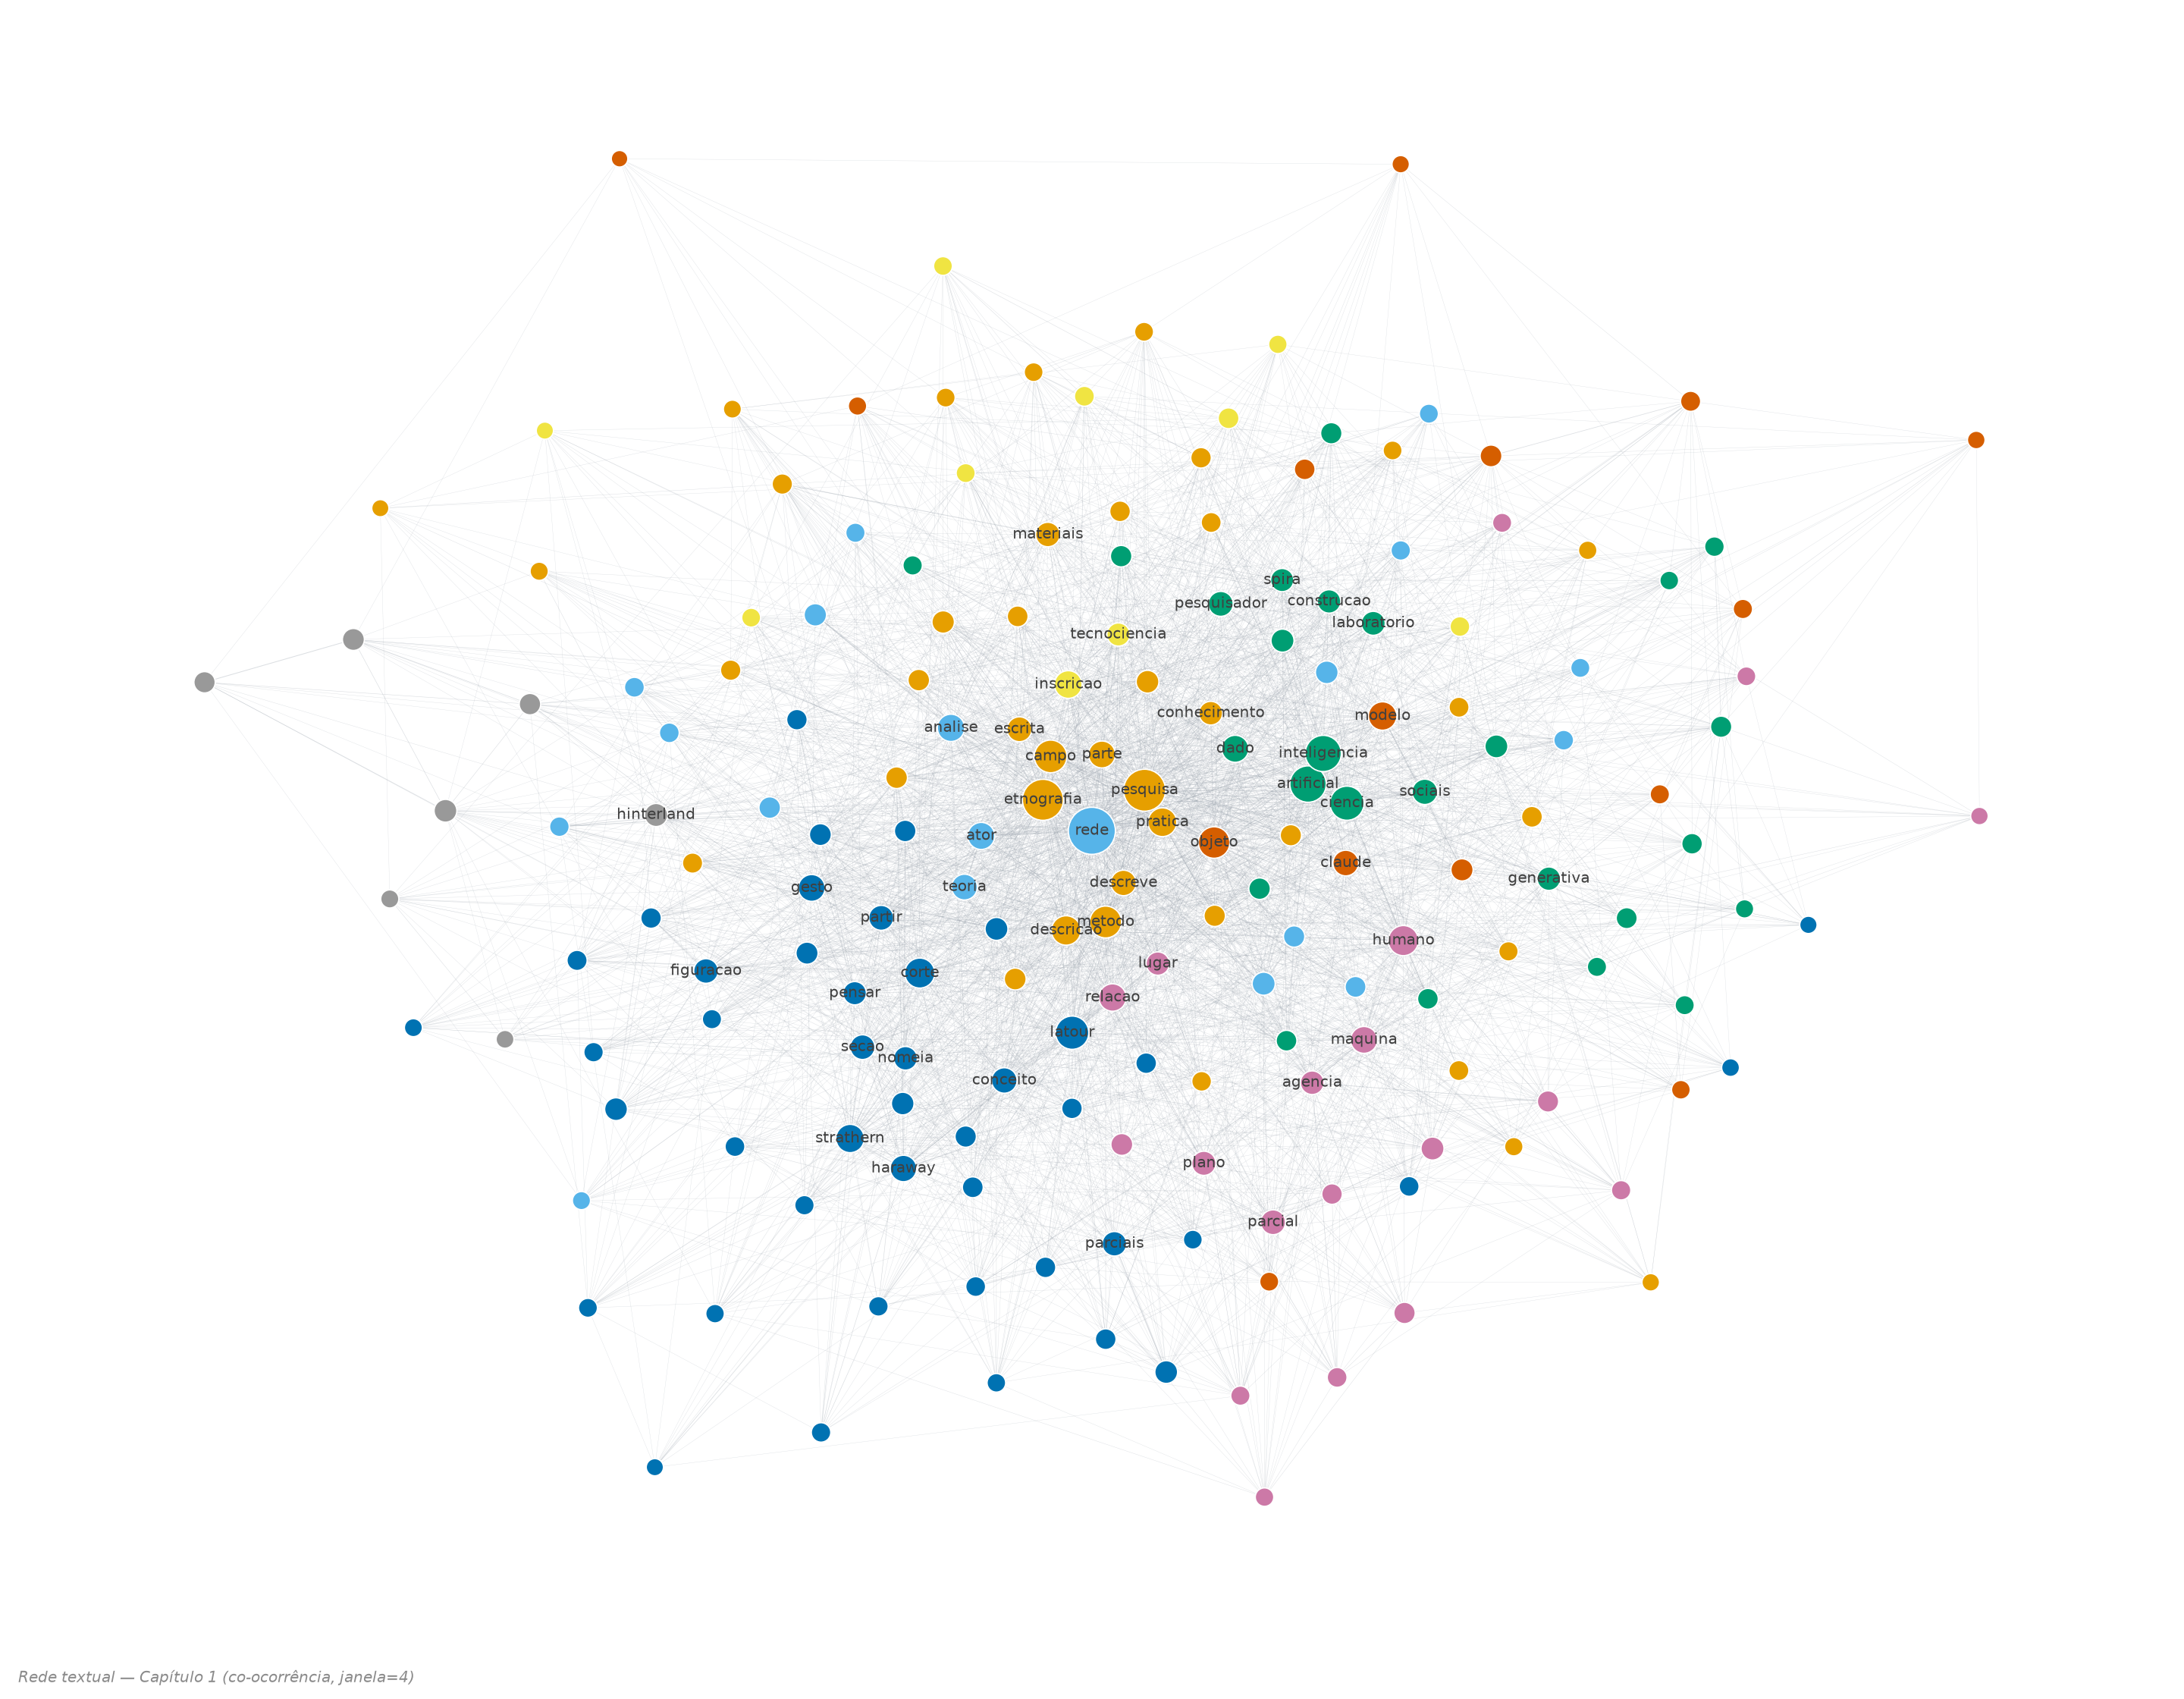
\includegraphics[width=1.0\textwidth,keepaspectratio]{figuras/cap.1/infranodus_cap1_network.png}
\caption[Rede textual completa do capítulo~\ref{capitulo1} (análise de rede textual)]{Rede textual completa do capítulo~\ref{capitulo1} (análise de rede textual, segundo \textcite{paranyushkin2019infranodus}). O grafo resulta de janela deslizante de 4 \textit{tokens} sobre o texto pré-processado (remoção de \textit{stopwords}, comandos \LaTeX, lematização leve), com pesos decrescentes pela distância (3-2-1). Os nós são os 180 termos de maior frequência mantidos no maior componente conectado após a filtragem de arestas com peso $<2$; o tamanho do nó é proporcional ao \textit{degree} ponderado e a cor indica a comunidade detectada por Louvain ponderado. Esta vista privilegia a estrutura geral do capítulo, incluindo termos periféricos e pontes entre tópicos. Arquivos auxiliares (\texttt{.gexf} para \texttt{Gephi}, CSVs, métricas e relatório) em \texttt{infranodus/} no repositório \url{https://github.com/julianehelanski/tecno-etnografia-centro-ia}.}
\label{fig:infranodus-cap1-network}
\end{figure}

A segunda inscrição reduz o grafo ao seu esqueleto semântico (figura~\ref{fig:infranodus-cap1-focus}) e me devolve, com clareza, a resposta à pergunta inicial. Mantenho apenas os 100 termos com maior \textit{degree} ponderado e as arestas mais densas. Os termos com maior peso são, em ordem, \textit{pesquisa}, \textit{ciência}, \textit{rede}, \textit{pesquisador(a)}, \textit{modelo}, \textit{humano}, \textit{objeto}, \textit{inteligência}, \textit{artificial}, \textit{campo} e \textit{etnografia}. Os termos que mais costuram comunidades distintas, isto é, com maior \textit{betweenness}, são \textit{ciência}, \textit{pesquisa}, \textit{rede} e \textit{pesquisador(a)}: termos genéricos que permitem o trânsito entre os campos conceituais da teoria ator-rede, das ciências sociais e da inteligência artificial. A condição de \textit{ponte}, no sentido que \textcite{Latour1986Visualization} dá ao termo, parece coincidir aqui com a condição de \textit{tradutor} no sentido latouriano mais amplo \parencite{Latour2011CienciaEmAcao}. A detecção de comunidades estabilizou seis tópicos latentes:\footnote{Os rótulos abaixo correspondem aos quatro a seis termos de maior \textit{degree} dentro de cada comunidade; preservo a forma lematizada produzida pelo \texttt{script} para evitar tradução interpretativa precoce.} (i)~\textit{escrita} e \textit{composição} em torno de \textit{pesquisador}, \textit{modelo}, \textit{objeto}, \textit{Claude}; (ii)~campo conceitual ator-rede em torno de \textit{rede}, \textit{Latour}, \textit{agência}, \textit{ator}, \textit{diagrama}, \textit{distribuída}; (iii)~ciências sociais e campo em torno de \textit{ciência}, \textit{sociais}, \textit{dado}, \textit{conhecimento}, \textit{cientista}; (iv)~IA e etnografia em torno de \textit{pesquisa}, \textit{inteligência}, \textit{artificial}, \textit{etnografia}, \textit{construção}, \textit{técnico}; (v)~humano-máquina-método em torno de \textit{humano}, \textit{método}, \textit{existência}, \textit{máquina}, \textit{parcial}; (vi)~um \textit{cluster} periférico em torno de \textit{Simondon}, \textit{técnica} e \textit{alienação}.

\begin{figure}[H]
\centering
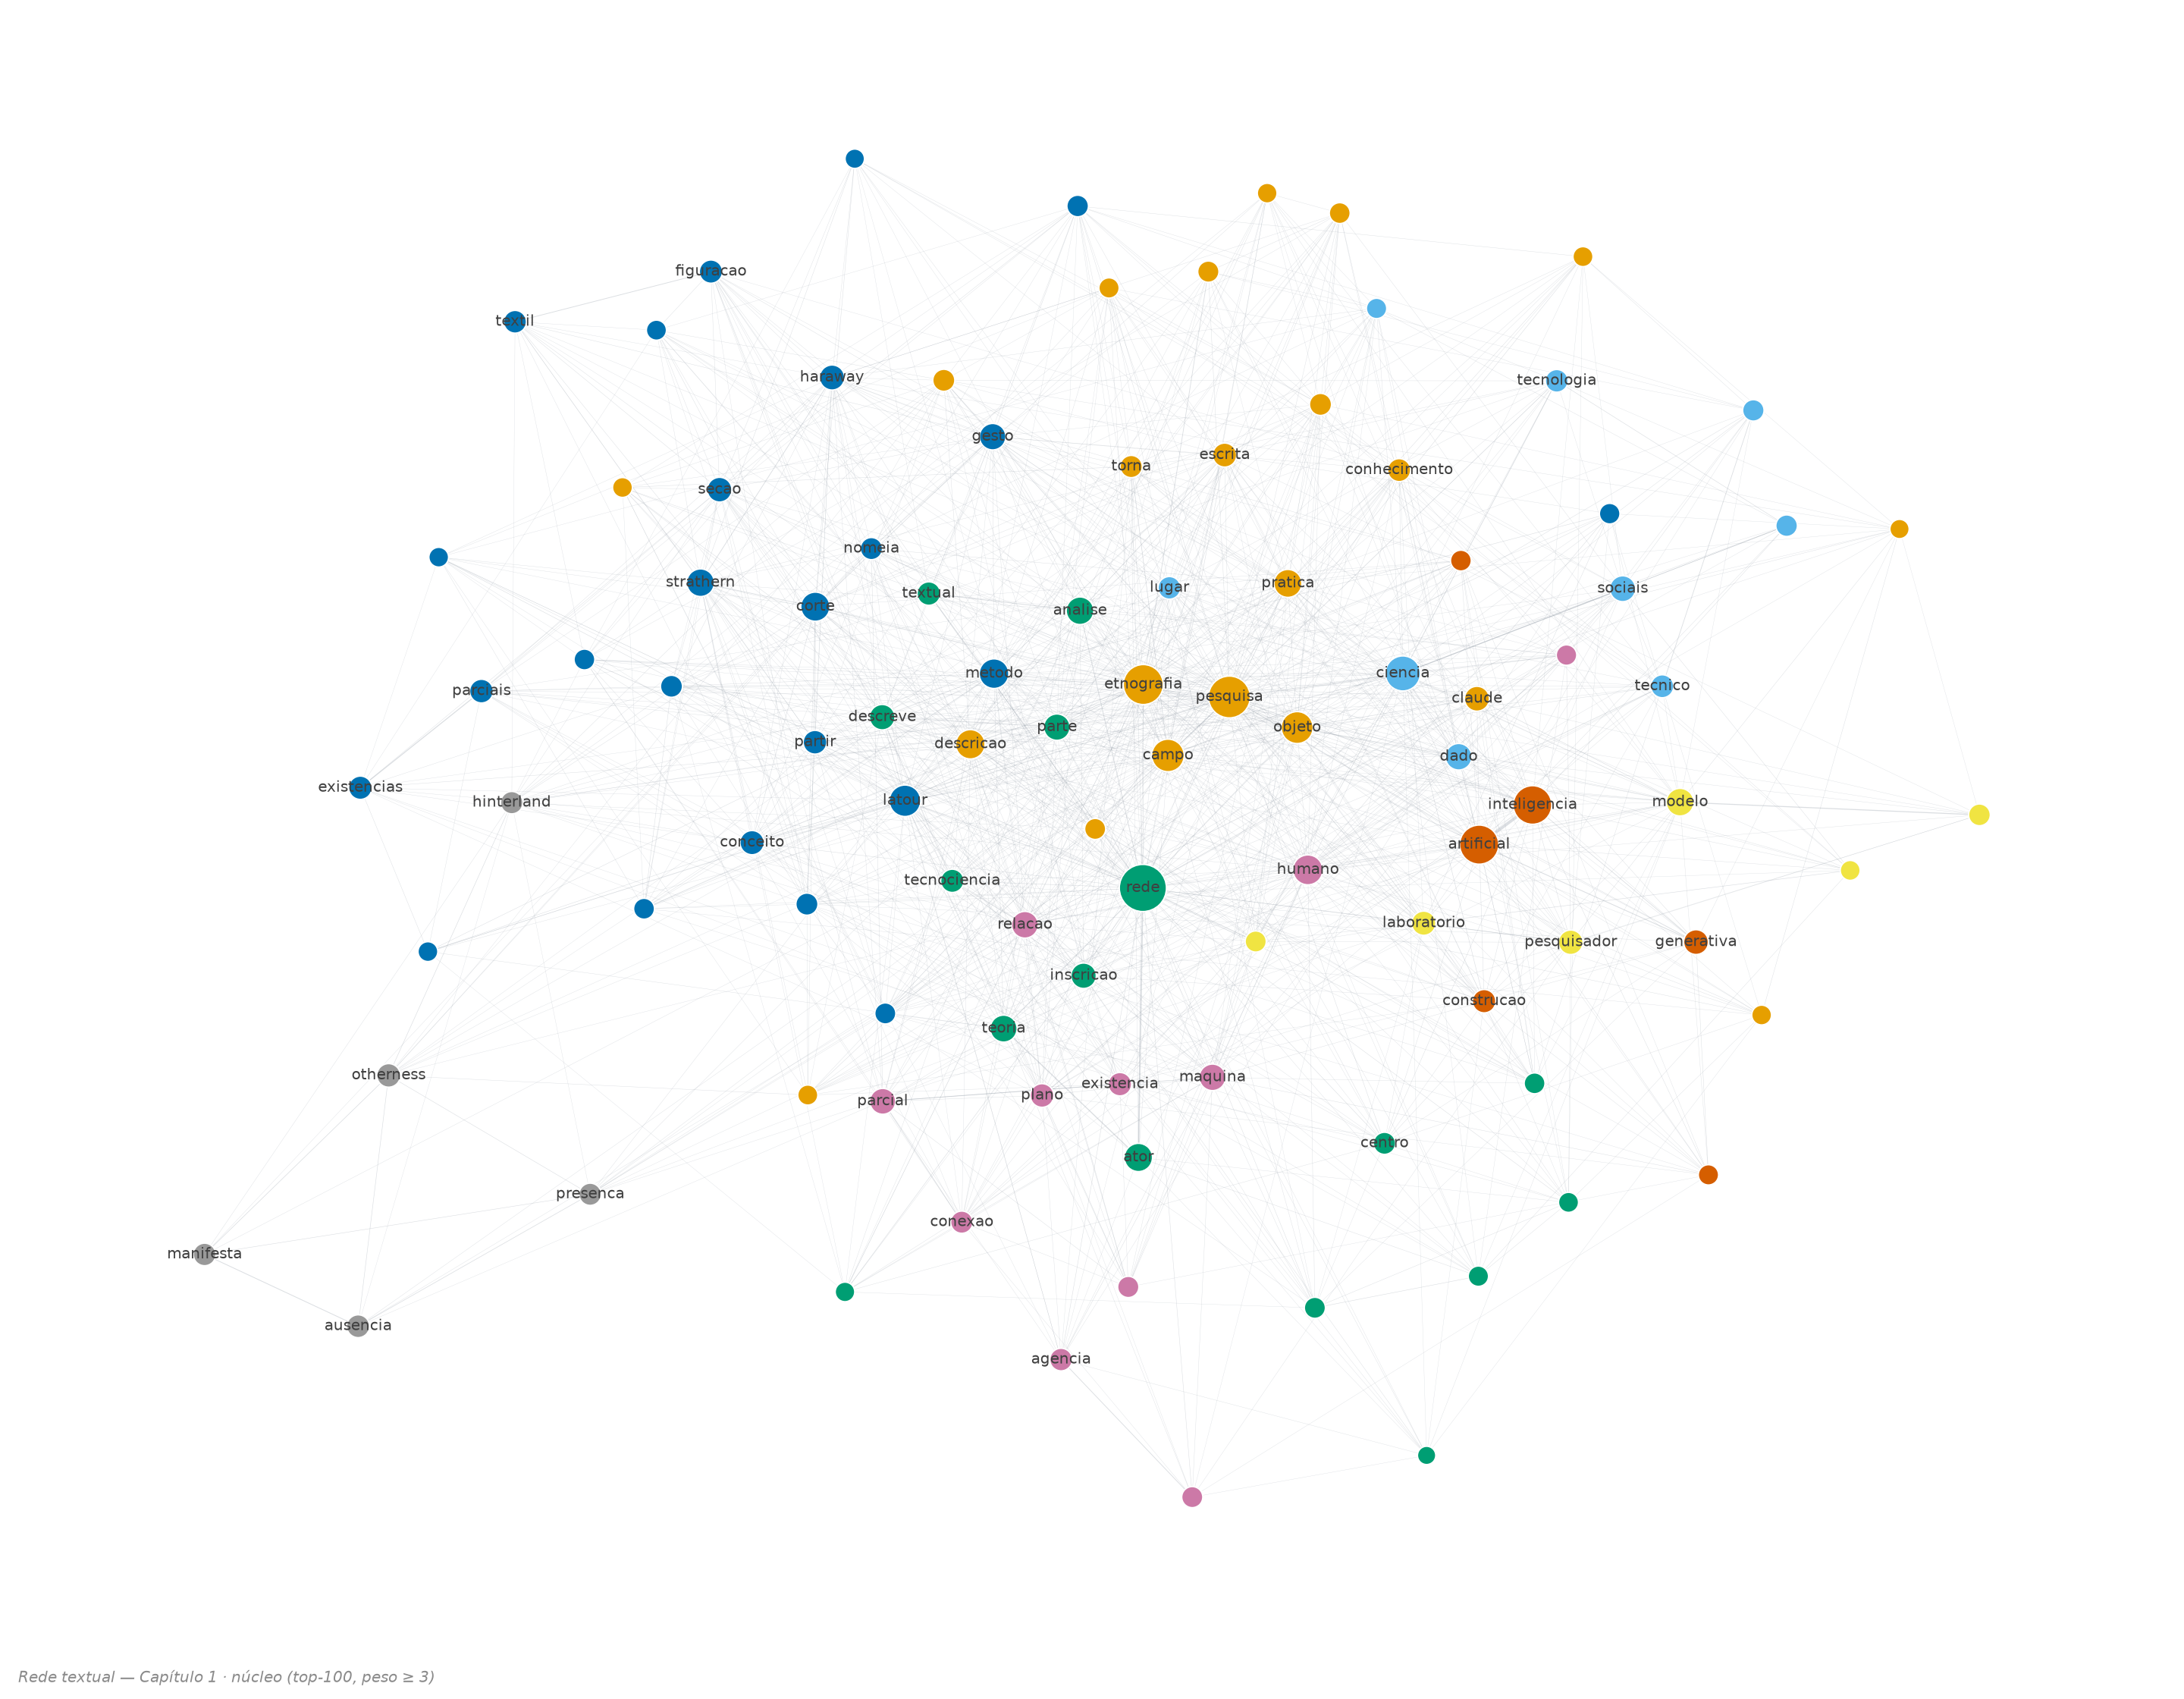
\includegraphics[width=1.0\textwidth,keepaspectratio]{figuras/cap.1/infranodus_cap1_focus.png}
\caption[Núcleo da rede textual do capítulo~\ref{capitulo1} (análise de rede textual)]{Núcleo da rede textual do capítulo~\ref{capitulo1} (análise de rede textual). Os nós são os 100 termos com maior \textit{degree} ponderado; o tamanho do nó é proporcional ao \textit{degree}; a cor indica a comunidade detectada por Louvain ponderado; arestas com peso $\geq 3$. Comparada à figura~\ref{fig:infranodus-cap1-network}, esta vista retém apenas o esqueleto semântico do capítulo, ou seja, os conceitos mais centrais e suas conexões fortes, sem a periferia. Versão de alta resolução, arquivo \texttt{.gexf} para o \texttt{Gephi} e relatório completo disponíveis em \texttt{infranodus/} no repositório \url{https://github.com/julianehelanski/tecno-etnografia-centro-ia}.}
\label{fig:infranodus-cap1-focus}
\end{figure}

A terceira inscrição muda o critério de peso (figura~\ref{fig:infranodus-cap1-focus-pmi}). Até aqui, o tamanho dos nós e a densidade das arestas refletiram a contagem ponderada, métrica que tende a inflar conceitos onipresentes cuja associação com qualquer outro termo é estatisticamente trivial. Aqui, ranqueio os mesmos 100 nós segundo critérios informacionais: o tamanho passa a ser proporcional ao \textit{PageRank}, que mede a centralidade na rede em vez da contagem bruta, e as arestas são filtradas pelo \textit{Normalized Pointwise Mutual Information} (NPMI), que retém apenas co-ocorrências surpreendentes dadas as frequências marginais de cada termo. O efeito é redistribuição da hierarquia textual: conceitos pouco frequentes e estrategicamente posicionados sobem para o primeiro plano, e termos onipresentes cuja vizinhança é previsível recuam. Quis essa inscrição justamente porque desconfiava da resposta da figura~\ref{fig:infranodus-cap1-focus}: termos como \textit{pesquisa} e \textit{ciência} pesam tanto que arriscam encobrir conexões mais específicas. A leitura comparada das duas figuras me devolve duas listas distintas do que tem peso no meu texto, e a diferença entre elas é informação metodologicamente carregada.

\begin{figure}[H]
\centering
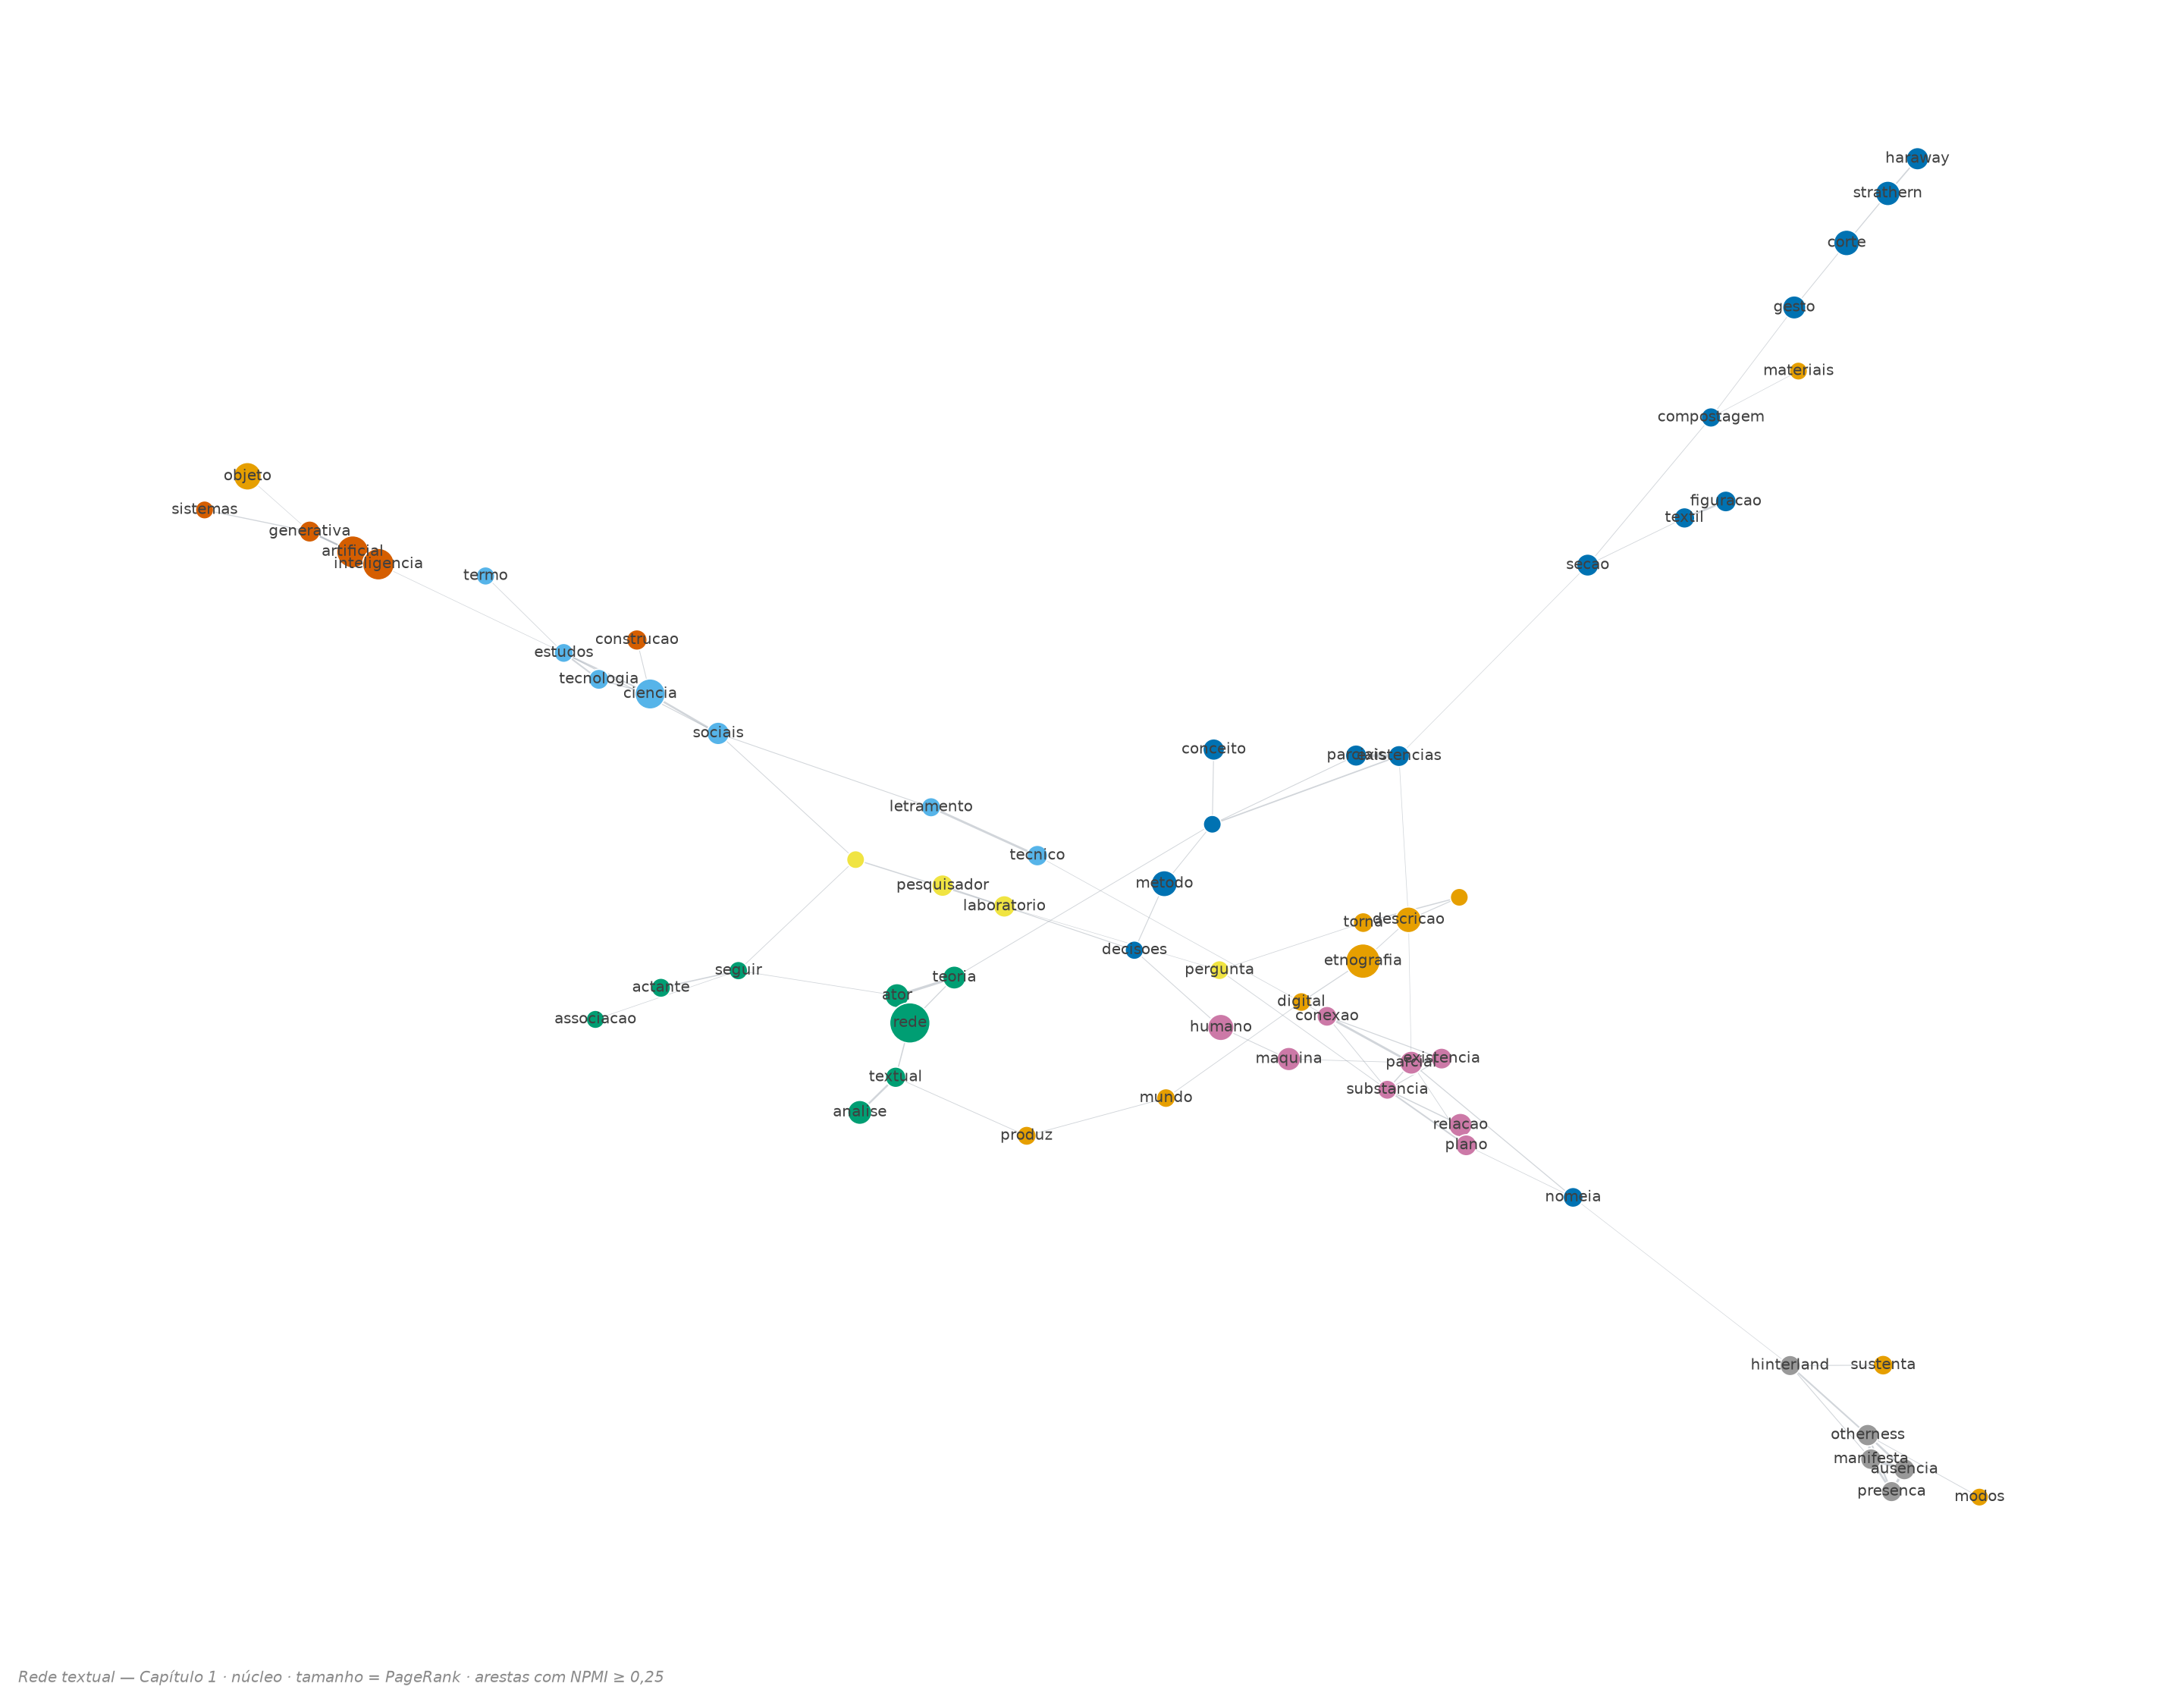
\includegraphics[width=1.0\textwidth,keepaspectratio]{figuras/cap.1/infranodus_cap1_focus_pmi.png}
\caption[Núcleo da rede textual do capítulo~\ref{capitulo1} ponderado por PageRank e NPMI]{Núcleo da rede textual do capítulo~\ref{capitulo1}, ranqueado por critérios informacionais em vez de frequentistas. Os mesmos 100 nós da figura~\ref{fig:infranodus-cap1-focus} são exibidos, mas o tamanho passa a ser proporcional ao \textit{PageRank} (centralidade na rede, em vez de contagem bruta) e as arestas são filtradas pelo \textit{Normalized Pointwise Mutual Information} (NPMI~$\geq 0{,}25$), retendo apenas co-ocorrências surpreendentes dadas as frequências marginais de cada termo. A cor mantém a comunidade Louvain. Esta vista promove conceitos pouco frequentes e estrategicamente posicionados, e deprime termos onipresentes cuja associação com qualquer outro é trivial, funcionando como contraponto à leitura puramente frequentista. Métricas e arquivo \texttt{.gexf} em \texttt{infranodus/} no repositório \url{https://github.com/julianehelanski/tecno-etnografia-centro-ia}.}
\label{fig:infranodus-cap1-focus-pmi}
\end{figure}

\medskip

As três inscrições seguintes mudam de pergunta. Em vez de \enquote{o que se liga a quê}, perguntam \enquote{quando cada conceito entra na minha argumentação, quanto tempo permanece em circulação, e como migra ao longo do capítulo}. Convertem o tempo da leitura, isto é, a ordem dos parágrafos, em eixo de análise. Eu precisava saber se os termos que pesam nas vistas sincrônicas pesam por persistência ou por concentração local, e essa pergunta não tem como ser respondida pelos grafos anteriores.

A quarta inscrição é o Gantt lexical (figura~\ref{fig:trajectory-gantt}). Cada linha do gráfico corresponde a um conceito, e cada barra horizontal marca a vida desse conceito no capítulo, do parágrafo de entrada ao parágrafo de saída. A inscrição me devolve informação que os grafos sincrônicos não ofereciam: existem conceitos que abro cedo e mantenho até o fim, existem conceitos que entram tarde e ficam pouco tempo, e existem conceitos que circulam por janela estreita de parágrafos antes de desaparecer. A leitura do Gantt traz autocrítica imediata: alguns dos termos com maior \textit{degree} nas vistas sincrônicas só existem em fração curta do capítulo, o que sugere que sua centralidade estrutural disfarça uma centralidade local. A inscrição expõe essa diferença sem que eu precise tematizá-la em prosa.

\begin{figure}[H]
\centering
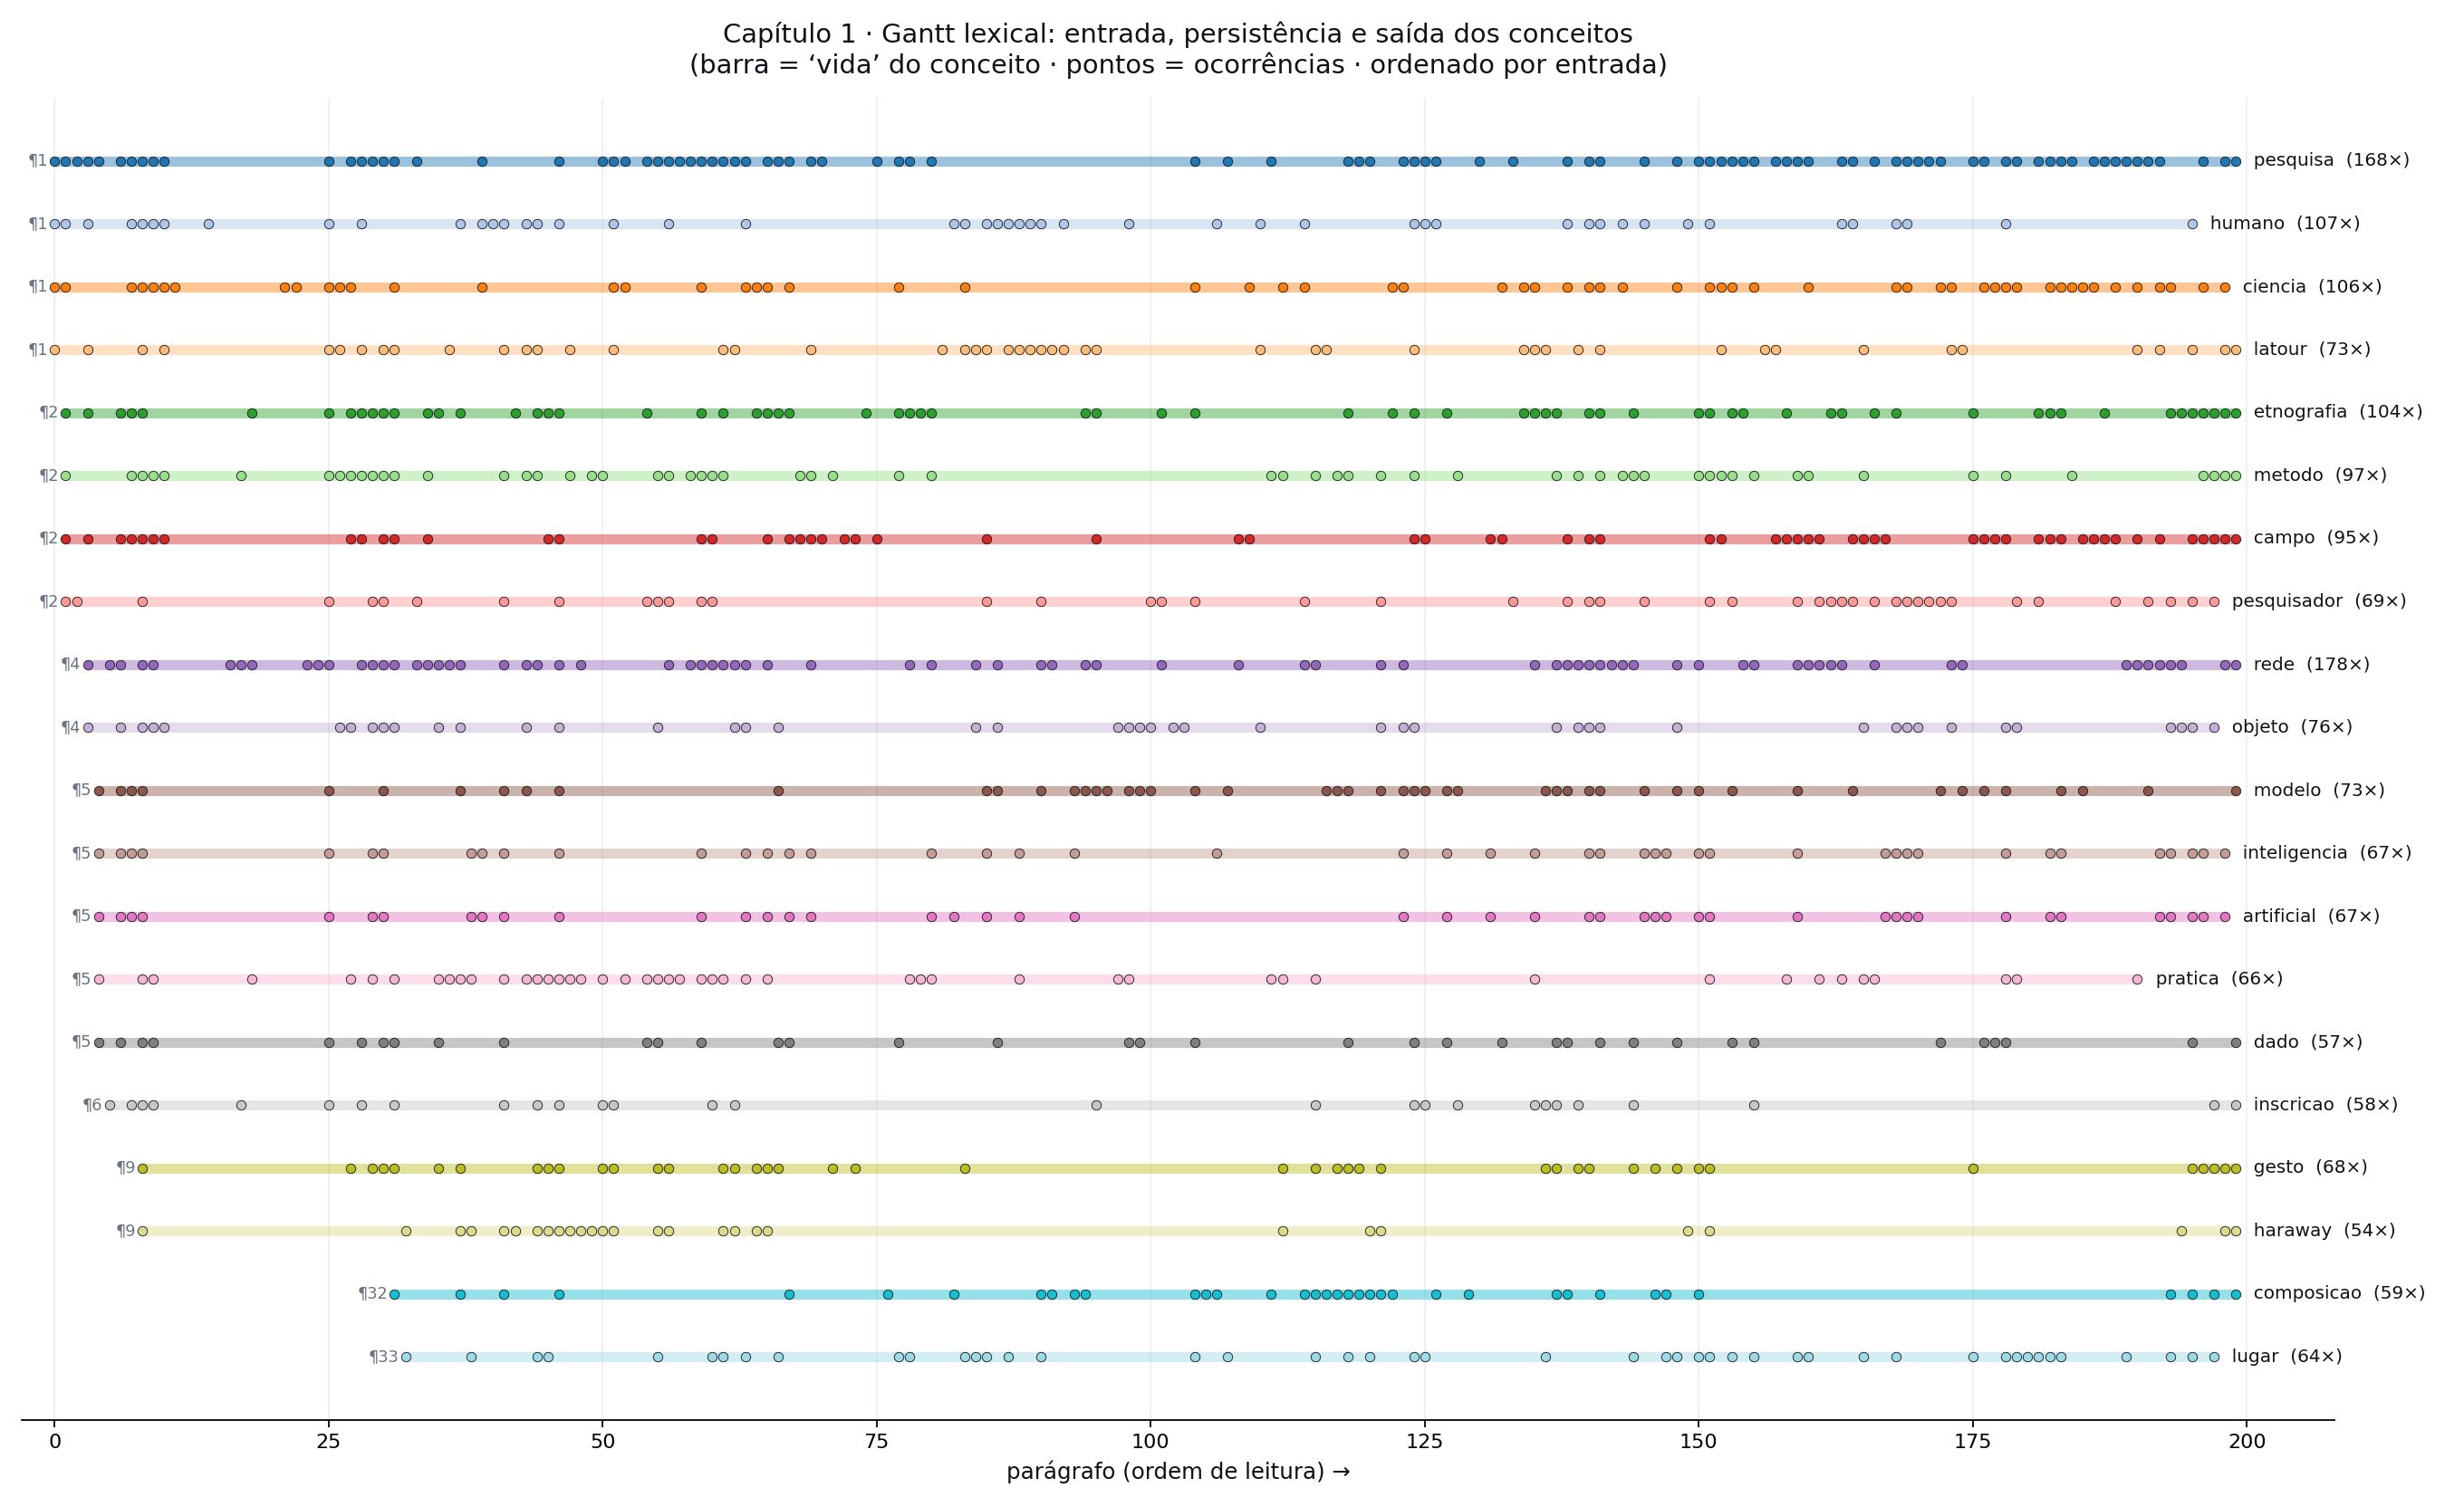
\includegraphics[width=1.0\textwidth,keepaspectratio]{figuras/cap.1/trajectory_gantt.png}
\caption[Gantt lexical do capítulo~\ref{capitulo1}: entrada, persistência e saída dos conceitos]{Gantt lexical do capítulo~\ref{capitulo1}. Cada linha corresponde a um dos 20 conceitos de maior frequência, excluídos termos genéricos e o marcador \texttt{claude}; o eixo horizontal é a ordem de leitura em parágrafos. A barra colorida marca a vida do conceito no capítulo, do parágrafo de primeira aparição (rótulo \P\textit{n}) ao último; os pontos sobre a barra indicam cada ocorrência; o número entre parênteses à direita é a contagem total. As linhas estão ordenadas por parágrafo de entrada, evidenciando a sequência em que cada noção é convocada e por quanto tempo permanece em circulação. Gerado pelo \textit{script} \texttt{narrative\_trajectory.py}, disponível em \url{https://github.com/julianehelanski/tecno-etnografia-centro-ia/tree/main/infranodus}.}
\label{fig:trajectory-gantt}
\end{figure}

A quinta inscrição refina a anterior por meio do fluxo aluvial (figura~\ref{fig:trajectory-alluvial}). Em vez de exibir cada conceito como entidade isolada, particiono o capítulo em oito segmentos sequenciais e mostro, em cada segmento, os cinco termos de maior frequência local. Faixas translúcidas conectam um termo a si mesmo quando ele persiste no \textit{top}-5 entre segmentos adjacentes, e setas marcam estreias.
O efeito visual é o de sucessão de paisagens conceituais que se sobrepõem parcialmente: alguns termos atravessam o capítulo inteiro, outros aparecem em apenas um segmento, e existem zonas de transição em que conjuntos conceituais inteiros são substituídos. A inscrição responde à pergunta que o Gantt deixa em aberto, qual seja, a de saber o que coexiste com o quê em cada momento da minha argumentação. Ela me mostra que o meu texto tem biografia: conceitos nascem, vivem com outros conceitos, e morrem, e essa biografia é parte do que dá peso aos termos nas vistas sincrônicas.

\begin{figure}[H]
\centering
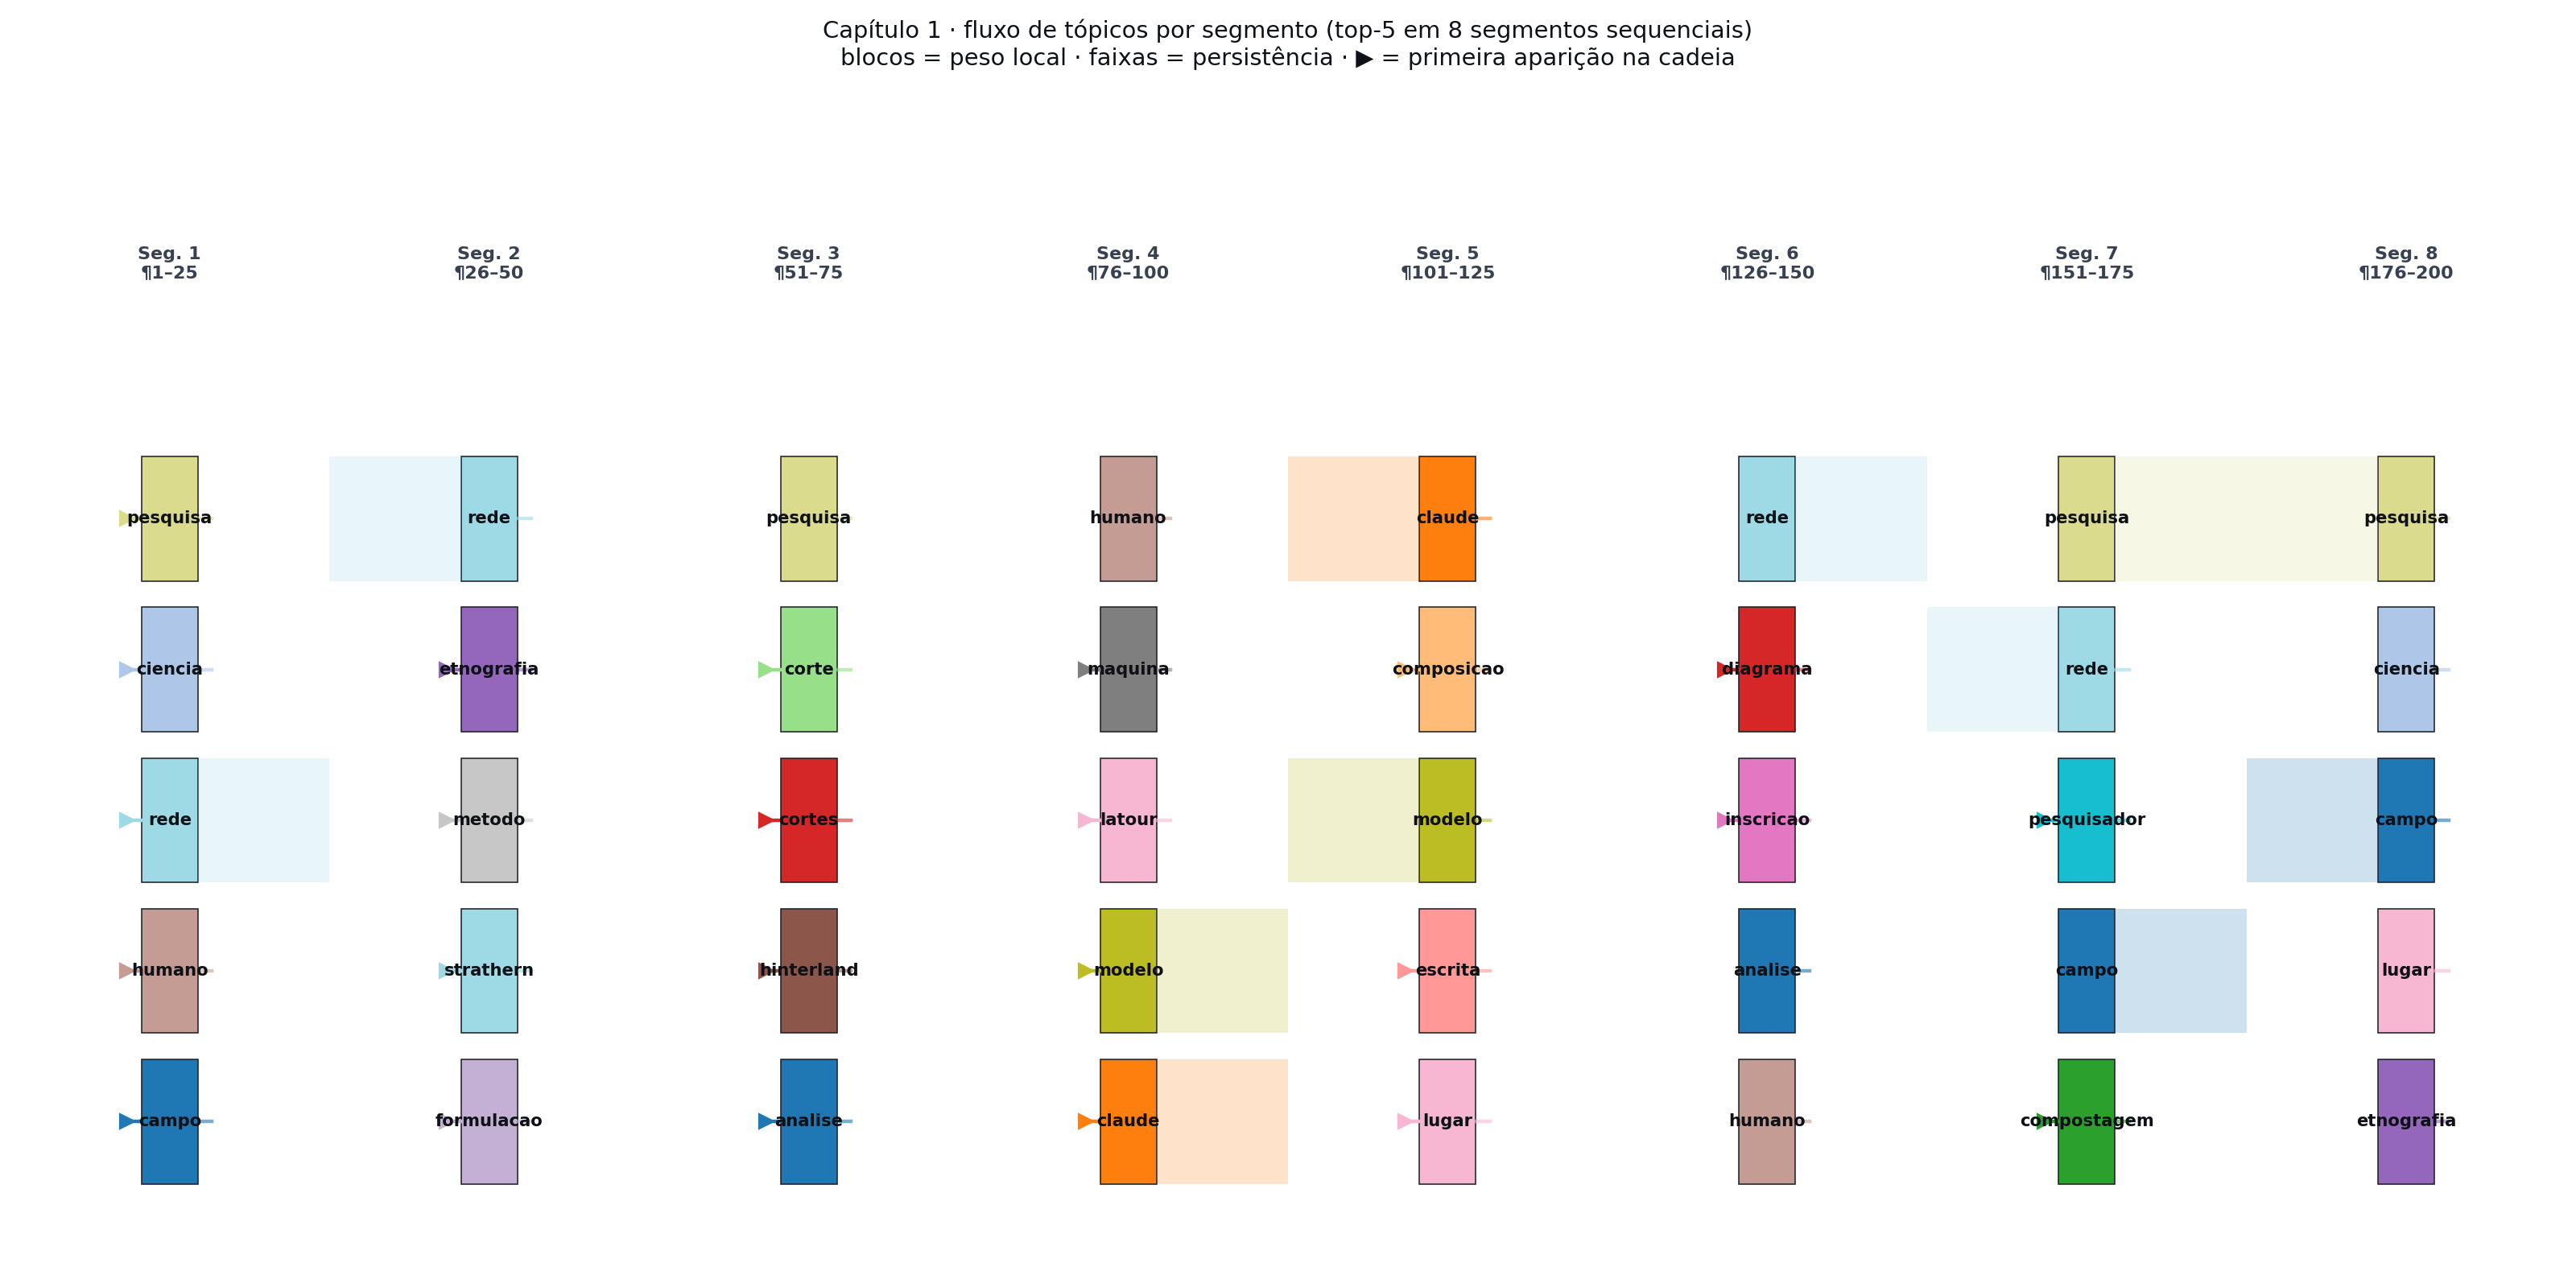
\includegraphics[width=1.0\textwidth,keepaspectratio]{figuras/cap.1/trajectory_alluvial.png}
\caption[Fluxo aluvial de tópicos ao longo do capítulo~\ref{capitulo1}]{Fluxo aluvial do capítulo~\ref{capitulo1}. O capítulo é particionado em 8 segmentos sequenciais de igual extensão em parágrafos (rótulos \P\textit{n}--\P\textit{m} no topo); em cada segmento são listados os 5 termos de maior frequência local (blocos coloridos, com a posição vertical refletindo o \textit{ranking} dentro do segmento). Faixas translúcidas conectam um termo a si mesmo entre segmentos adjacentes quando ele persiste no \textit{top}-5, materializando continuidades temáticas; setas $\blacktriangleright$ assinalam a primeira aparição de um conceito na cadeia. A figura responde à pergunta \enquote{o que se liga a quê ao longo do capítulo} e torna visíveis tanto os tópicos persistentes quanto as entradas tardias e saídas precoces. Gerado pelo \textit{script} \texttt{narrative\_trajectory.py}, disponível em \url{https://github.com/julianehelanski/tecno-etnografia-centro-ia/tree/main/infranodus}.}
\label{fig:trajectory-alluvial}
\end{figure}

A sexta inscrição opera por compressão ainda mais radical (figura~\ref{fig:trajectory-semantic}). Agrupo os parágrafos em \textit{momentos} de cinco parágrafos consecutivos, vetorizo cada momento por TF-IDF sobre unigramas e bigramas, e projeto a sequência inteira em duas dimensões obtidas por PCA aplicado ao resultado de redução prévia por \textit{Truncated SVD}. O que aparece no plano é trajetória: cada ponto é um momento, as setas seguem a ordem de leitura, e a distância entre pontos aproxima a dissimilaridade lexical entre eles. Deslocamentos longos indicam mudanças temáticas; voltas curtas indicam que retomei campo semântico já visitado. Essa última inscrição me devolve, em vista única e legível de cima, o movimento argumentativo do capítulo: posso rastrear, sem precisar reler tudo, em que ponto da exposição abri um problema, em que ponto voltei a ele, e em que momento o capítulo se distanciou mais de seu próprio começo.

\begin{figure}[H]
\centering
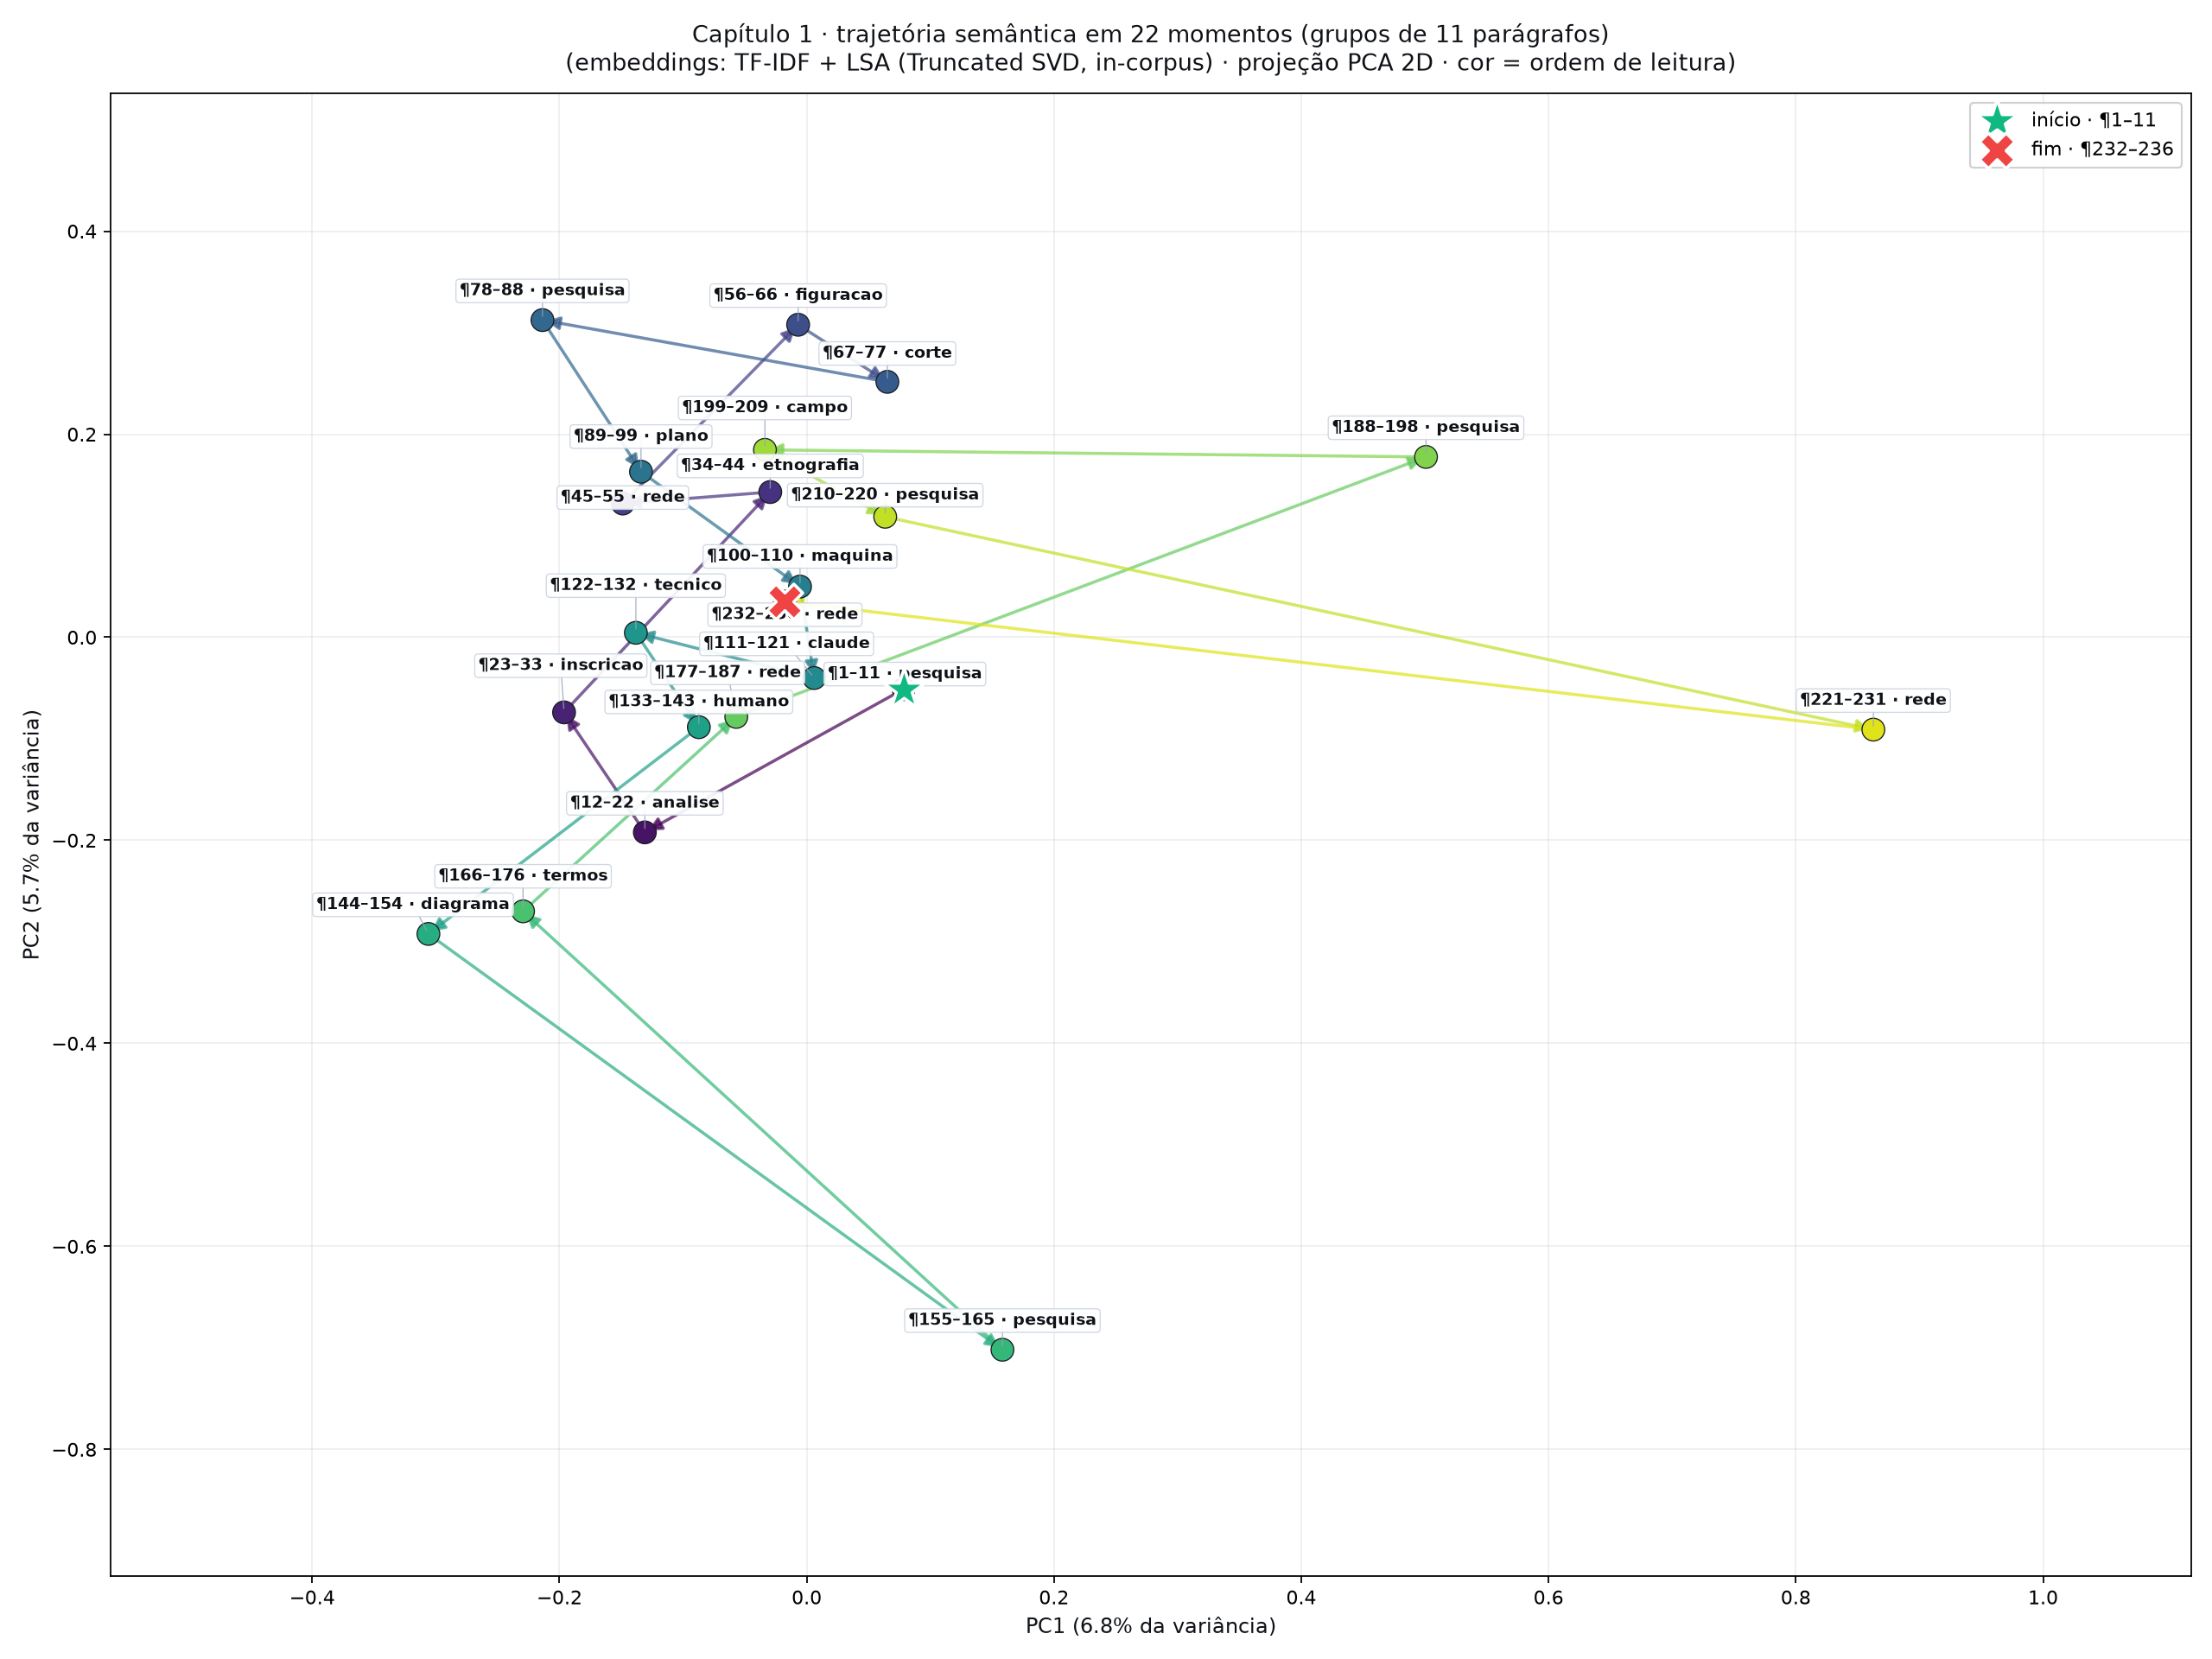
\includegraphics[width=1.0\textwidth,keepaspectratio]{figuras/cap.1/trajectory_semantic.png}
\caption[Trajetória semântica do capítulo~\ref{capitulo1}]{Trajetória semântica do capítulo~\ref{capitulo1}. Os parágrafos são agrupados em \textit{momentos} de 5 parágrafos consecutivos; cada momento é vetorizado por \textit{TF-IDF} (unigramas e bigramas) seguido de redução por \textit{Truncated SVD} (\textit{Latent Semantic Analysis} \textit{in-corpus}, \textit{fallback} usado quando o \textit{sentence-transformer} multilíngue não está disponível) e projetado em duas dimensões por PCA. Cada ponto é um momento, rotulado com o intervalo de parágrafos e o termo dominante; as setas seguem a ordem de leitura, com gradiente \textit{viridis} do início ($\star$ verde) ao fim ($\times$ vermelho). Distâncias no plano aproximam dissimilaridade lexical entre momentos; deslocamentos longos indicam mudanças temáticas, voltas curtas indicam retomada de campo semântico já visitado. O percentual de variância explicada por cada eixo aparece nos rótulos. Gerado pelo \textit{script} \texttt{narrative\_trajectory.py}, disponível em \url{https://github.com/julianehelanski/tecno-etnografia-centro-ia/tree/main/infranodus}.}
\label{fig:trajectory-semantic}
\end{figure}

\medskip

Lidas em série, as seis inscrições tecnocientíficas me devolveram três chamadas de atenção sobre o que pesa e o que conecta no meu texto. A primeira é confirmação modesta: os termos que se mostram centrais nas três vistas sincrônicas coincidem com os conceitos que convoco explicitamente, e os termos com maior intermediação são os mais genéricos do capítulo, o que sugere que minha costura argumentativa está sendo feita por palavras-coringa que ainda esperam ser teorizadas com mais força. A segunda é surpresa que aparece nas seis figuras de modos distintos: as duas comunidades com a ligação ponderada mais fraca entre si são a das ciências sociais (Tópico~iii) e a do par humano-máquina-método (Tópico~v); o Gantt e o aluvial mostram, além disso, que essas duas famílias de termos têm biografias temporais distintas no capítulo, ocupando segmentos parcialmente disjuntos da minha exposição.
A formulação de \textcite{Law2004After} sobre o \textit{method assemblage} me ajuda a nomear o que isso quer dizer: a \textit{Otherness} apagada para que a presença se sustente é, neste capítulo, a conexão entre os dois conjuntos conceituais que ainda preciso fazer trabalhar juntos. A terceira chamada diz respeito ao \textit{cluster} periférico em torno de Simondon: ele aparece na rede expandida (figura~\ref{fig:infranodus-cap1-network}), some no núcleo frequentista (figura~\ref{fig:infranodus-cap1-focus}), reaparece na vista informacional (figura~\ref{fig:infranodus-cap1-focus-pmi}) e ocupa janela curta no Gantt (figura~\ref{fig:trajectory-gantt}), sinalizando promessa teórica que abro aqui e que os capítulos subsequentes precisam costurar à rede maior, sob risco de virar nota de rodapé errante.

Reconheço o paradoxo do gesto. Aplicar análise de rede a um capítulo que invoca a teoria ator-rede arrisca tomar a metáfora pelo método; e a similaridade entre os dois usos da palavra \textit{rede} é superficial, dado que a rede ator-rede é cadeia de associações heterogêneas e ontologicamente plana, e as redes textuais aqui geradas são grafos bidimensionais de co-ocorrências de \textit{tokens} ponderados por proximidade.\footnote{A confusão entre os dois sentidos de \textit{rede} é discutida por \textcite[pp.~129--132]{Latour2007Reassembling}, que distingue \textit{rede} como ferramenta de inscrição e como diagnóstico ontológico. Mantenho a distinção: o que a análise de rede textual e os meus \textit{scripts} de trajetória produzem são inscrições tecnocientíficas; o que minha tese descreve, ela própria, são redes sociotécnicas.} As seis inscrições funcionaram como instrumento de leitura que eu não teria conseguido produzir só com olhos humanos e releituras sucessivas. Cada uma ordena, hierarquiza, inclui e exclui, e o conjunto delas me serviu para localizar o que pesa, o que liga, o que persiste e o que migra na argumentação que costurei. É essa experimentação tecnoetnográfica, e o que ela me devolveu, que justifica sua presença aqui.

\subsection{Cosmotécnica e situacionalidade}

Devo situar essa escolha. Ninguém é obrigado a usar inteligência artificial para fazer pesquisa acadêmica. Há muitas maneiras de fazer uma pesquisa, e nem todas produzem bons resultados, inclusive quando não envolvem tecnologias tão polêmicas quanto a IA. É também verdade que parte dos pesquisadores que recorrem a modelos de linguagem o faz para poupar-se do trabalho intelectual, delegando à máquina o que deveria ser exercício de pensamento,\footnote{Em 6 de março de 2026, o CNPq publicou a Portaria n.º~2.664, que institui a Política de Integridade na Atividade Científica. O Art.~9, inciso~I, alínea~c, determina que pesquisadores declarem o uso de ferramentas de Inteligência Artificial Generativa em qualquer fase do desenvolvimento da pesquisa, especificando a ferramenta utilizada e a finalidade. A alínea~d veda a submissão de conteúdo gerado por IAG como se fosse de autoria humana, atribuindo responsabilidade integral aos autores pelo conteúdo final. Minha tese antecipou, por escolha metodológica, o que a norma agora regula. Disponível em: \url{http://memoria2.cnpq.br/web/guest/view/-/journal_content/56_INSTANCE_0oED/10157/23142775?COMPANY_ID=10132}. Acesso em: 13 mar. 2026.} e os problemas decorrentes dessa delegação já são amplamente conhecidos: textos genéricos, argumentos circulares, referências fabricadas, perda de voz autoral.

Minha tese procura responder a essas três perguntas de modo explícito. O \textit{por que} decorre das condições materiais descritas acima e da coerência com o próprio referencial teórico (estudar existências parciais com uma existência parcial). O \textit{como} está documentado nesta seção e no apêndice~\ref{apendice:colaboracao-ia}. O \textit{qual} atravessa os capítulos que se seguem. Meu fazer-com o \texttt{claude} é, antes de tudo, experimentação antropológica: uma etnógrafa que estuda como cientistas e engenheiros constroem inteligência artificial decide construir sua própria tese com inteligência artificial, submetendo-se às mesmas mediações, opacidades e negociações que observa em seus interlocutores. O gesto é epistêmico e produz conhecimento sobre a IA pela experiência de fazer-com ela, com todos os riscos que esse fazer-com implica.

E se levarmos a sério o argumento de Yuk Hui, esse fazer-com não é generalizável.\footnote{Vicentin conecta a proposta de Simondon de aprofundamento da tecnologia com a defesa de Yuk Hui de que, em lugar de axiomatizar a moral, precisaremos voltar aos modos de conhecimento diferentes que ainda não foram considerados por engenheiros e acadêmicos que trabalham com inteligência artificial \parencite[p.~186]{hui2020tecnodiversidade}. Essa convergência tem peso para meu argumento: se o aprofundamento da IA passa pela conexão entre o fazer técnico especializado e o conhecimento sócio-histórico sobre a tecnologia, então o fazer-com a IA na escrita desta tese pode ser interpretado como experimentação situada nos termos em que Hui concebe a cosmotécnica.} Hui propõe o conceito de cosmotécnica para desafiar a ideia de que a tecnologia seria categoria antropológica única e homogênea: a técnica é sempre a unificação entre uma ordem cósmica e uma ordem moral através de atividades técnicas, e portanto varia ontológica e cosmologicamente entre diferentes sociedades, em lugar de variar apenas funcional ou esteticamente.\footnote{Hui desenvolve o conceito de cosmotécnica em \textit{The Question Concerning Technology in China} \parencite{hui2016china}, onde demonstra que a técnica pode orientar-se pela harmonia com uma cosmologia moral, sem buscar necessariamente a eficiência mecânica. Hui chama essa possibilidade de tecnodiversidade: contra o monotecnologismo moderno, o reconhecimento de que existem múltiplas cosmotécnicas que permitem diferentes formas de vida social, política e estética \parencite{hui2020tecnodiversidade}.}

O quadro herdado da filosofia moderna pós-iluminista trata a tecnologia como conjunto de ferramentas universais e neutras destinadas à exteriorização da memória e à superação dos limites orgânicos. A cosmotécnica recusa essa universalidade: diferentes cosmologias produzem diferentes modos de compor com objetos técnicos, e quem pretende moldar o universal submete o mundo à sua própria cosmovisão. Ora, se há cosmotécnicas situadas, em lugar de a tecnologia, então o modo como eu, antropóloga brasileira, formada na tradição dos estudos de ciência e tecnologia latino-americanos, faço esta tese junto a um modelo de linguagem treinado predominantemente em dados anglófonos para produzir uma tese em português sobre redes tecnocientíficas é, ele próprio, gesto cosmotécnico particular: forma específica de unificar ordem epistêmica e atividade técnica que não se repete em outros contextos, outras tradições, outras cosmologias. A experimentação que documento nestas páginas é, portanto, modo de usar IA na pesquisa acadêmica, situado, parcial e responsável por seus próprios efeitos.

\section{Compostagens: compostar-com e tornar-se-com}
\label{sec:compostagens}

\epigrafe{%
Somos composto, não pós-humanos; habitamos as humusidades, não as humanidades. Filosofica e materialmente, sou compostista, não pós-humanista. Os bichos (humanos e não humanos) estão em devir-com mútuo e em todos os registros de tempo e de coisas, em emaranhados simpoiéticos, em mundificações e desmundicações terrenas, ecológicas e evolutivas do desenvolvimento.}%
{Donna Haraway, \textit{Ficar com o problema: fazer parentes no Chthuluceno}, 2023, p.~191.}

\epigrafe{%
It matters what thoughts think thoughts. It matters what knowledges know knowledges. It matters what relations relate relations. It matters what worlds world worlds. It matters what stories tell stories.}%
{Donna Haraway, \textit{Staying with the Trouble: Making Kin in the Chthulucene}, 2016 \parencite[p.~35]{Haraway2023Ficar}.}

A epígrafe que Haraway formulou \parencite[p.~35]{Haraway2023Ficar} anuncia a prática da compostagem como gesto epistemológico. Quando Haraway escreve que importa quais pensamentos pensam pensamentos, ela credita a Marilyn Strathern a formulação de que importa quais ideias usamos para pensar outras ideias. Esse é o registro próprio desta seção. Cada compostagem aqui descrita é momento em que materiais heterogêneos da minha pesquisa foram postos em camadas e fermentaram juntos, e nessa fermentação aprenderam uns dos outros como pensar uns com os outros. A operação que isto nomeia é distinta do gesto epistêmico do corte trabalhado na seção~\ref{sec:etnografia-heterodoxa}, pois não responde à pergunta sobre onde delimitar a rede para torná-la descritível. Aqui a pergunta é outra, isto é, que materiais empíricos e teóricos vieram parar juntos em minha pesquisa, em que ordem, com que efeitos recíprocos, e por que essas fermentações específicas tornaram possível o tipo de descrição etnográfica que esta tese sustenta. A compostagem trabalha como prática filosófica e material, e a posição de compostista que Haraway reivindica para si \parencite[p.~101]{Haraway2016Staying} é a posição que assumo aqui ao narrar as quatro fermentações que minha pesquisa precisou atravessar.

Minha etnografia acabou produzindo também outro modo de conhecimento que figura como \textit{compostagem}.\footnote{Cheguei ao termo \textit{compostagem} depois de tentar sem sucesso outros nomes para o que essas misturas significaram em minha pesquisa. \textit{Lições} foi a primeira tentativa, e descartei-a porque o vocabulário da lição supõe quem ensina e quem aprende, conteúdos definidos a transmitir, e direção da matéria do mestre para o aprendiz. A pesquisa não se passou assim. \textit{Aprendizagens} carregava o mesmo problema. O que aconteceu foi outra coisa, mais próxima do que \textcite{Haraway2023Ficar} nomeia como compostagem: camadas de materiais heterogêneos postas a fermentar ao longo dos anos, em que nenhum dos elementos pôde ser identificado como o conteúdo a ser transmitido nem como a posição que ensinava. Quatro deslizamentos da palavra organizam meu gesto argumentativo nesta seção. O primeiro é o gesto de Haraway de propor o composto no lugar do pós-humano: \enquote{somos húmus, não Homo, não anthropos; somos compostagem, não pós-humanos} \parencite[p.~32]{Haraway2016Staying}. A formulação foi sugerida a Haraway por Rusten Hogness e a autora descreve seu encontro com ela como pular numa pilha vermicular: \enquote{I jumped into that wormy pile} \parencite[p.~32]{Haraway2016Staying}. A figura recusa o humano-como-Homo em favor do humano-como-húmus, território fértil em que matérias heterogêneas se encontram e se transformam umas às outras. O segundo é a sympoiese, palavra que Haraway adota a partir da tese de Beth Dempster sobre sistemas \enquote{coletivamente produtores} sem fronteiras espaciais ou temporais autodefinidas, e que ela traduz como \textit{making-with}, fazer-com, em contraste com a autopoiese: \enquote{Sympoiesis is a simple word; it means `making-with.' Nothing makes itself; nothing is really autopoietic or self-organizing} \parencite[p.~58]{Haraway2016Staying}. Nada se faz sozinho, e o fazer é sempre em companhia. O terceiro é o par compostar-decompor, formulado por Haraway como prática conjunta de \textit{critters} humanos e não humanos que se compostam e decompõem uns aos outros, em todo tempo e matéria. A compostagem é gesto de juntar e gesto de desfazer, e nesse duplo gesto se ganha a fertilidade do composto. O quarto é a posição que Haraway reivindica: \enquote{I am a compostist, not a posthumanist} \parencite[p.~101]{Haraway2016Staying}. Compostista nomeia prática filosófica e material em curso, em lugar de identidade estabilizada. Dois traços do vocabulário haraweano importam para o uso que faço aqui. O primeiro é a metáfora da pilha quente. Haraway descreve sua leitura de Strathern como \enquote{I compost my soul in this hot pile} \parencite[p.~34]{Haraway2016Staying}, formulação que a tradução brasileira gloseia como \enquote{compostagem intelectual} e que o original nomeia em chave mais visceral, da pilha em fermentação. O segundo é a descrição que Haraway faz do próprio livro nos seus agradecimentos: \enquote{Cooking over many years, the compost pile of colleagues, students, and friends who have made this book possible is promiscuous, layered, and hot} \parencite[p.~ix]{Haraway2016Staying}. Cozinhando ao longo dos anos, em camadas, promíscua e quente: nesse sentido convoco aqui a compostagem para nomear o que aconteceu na minha pesquisa. Cada compostagem desta seção inscreve um momento em que materiais inicialmente mantidos separados pelo desenho da pesquisa precisaram ser postos a fermentar juntos, e em que essa fermentação implicou também a decomposição das partições prévias. A compostagem que mobilizo aqui tem afinidade com a articulação que Haraway desenvolve em torno de \textit{thinking-with} como \textit{becoming-with} \parencite[p.~33]{Haraway2016Staying}: pensar com funciona como tornar-se com, em vez de funcionar como aprender com.} As compostagens são um tipo de contribuição analítica desta tese para a etnografia de práticas tecnocientíficas envolvendo inteligência artificial, em especial a pesquisa em IA feita pelos pesquisadores, com eles e com IA (feita por mim com inteligência artificial). Essas compostagens não estavam previstas no desenho da pesquisa, e emergiram do encontro entre meu campo e os referenciais teóricos que convoquei ao longo do percurso. Cada uma nomeia uma mistura específica de materiais heterogêneos que precisaram fermentar juntos para que a descrição se tornasse possível. A primeira composta a regra latouriana de estudar a ciência em construção com a dispersão característica da pesquisa em IA, na qual não há laboratório centralizado a observar. A segunda composta o vocabulário da simetria metodológica com a especificidade da inteligência artificial generativa, e nessa fermentação decompõe a partição humano/não humano em existências parciais. A terceira composta minha formação em ciências sociais com o letramento técnico que o campo me exigiu, fazendo dessa fermentação parte da própria etnografia. A quarta composta a separação prévia entre ciência e política com a evidência empírica de que a pesquisa em IA, no \texttt{C4AI}, é simultaneamente decisão epistêmica e captação de recursos.

\subsection{Compostando o método: acompanhar a pesquisa em IA enquanto ciência em construção}
\label{subsec:compostagem1}

A primeira regra metodológica que Latour propõe \parencite{Latour2011CienciaEmAcao}, reproduzida e discutida na seção~\ref{sec:regras-metodologicas} deste capítulo, foi a regra que orientou minha entrada no campo. Decidir investigar a pesquisa em IA como ciência em construção foi convergência entre intuição de pesquisa e regra metodológica que se revelou adequada à medida que o campo se desdobrava diante de mim. Quando cheguei ao \texttt{C4AI} em 2022, o Centro tinha menos de dois anos de existência. Projetos como o \texttt{Spira} estavam em pleno desenvolvimento, a parceria com a \texttt{IBM} ainda parecia sólida, e as definições sobre o que o Centro seria e produziria estavam em disputa.\footnote{O relatório científico do período agosto de 2021 a julho de 2022 inscreve projetos em cinco desafios: no NLP2, o Corpus Carolina (650 milhões de \textit{tokens}), \textit{datasets} CORAA (290 horas de áudio) e Porttinari Treebank (12.000 sentenças anotadas); no BLAB (Computação Bio-In\texttt{Spira}da e Aprendizado de Máquina, designação que na configuração consolidada após 2023 corresponde aos desafios OceanML e KEML descritos na Tabela~\ref{tab:projetos_c4ai}), arquitetura modular sobre a Amazônia Azul; em Saúde, segmentação de lesões de AVC e identificação de pneumonia por Covid-19; no AgriBio, geoMULTIMAPS para análise de insegurança alimentar; e no AI Humanities, alinhamento do Observatório de IA ao NIC.br e aplicativos de robótica social. Nenhum estava concluído, e todos envolviam negociações ativas sobre escopo, método e recursos.}

O que eu encontrei foram pesquisadores negociando recursos, redefinindo escopos, improvisando infraestruturas, testando modelos que falhavam, justificando escolhas metodológicas para públicos diversos, em lugar de ciência pronta para estudar. Tratava-se de chegar à pesquisa em IA enquanto seus fatos e artefatos ainda não haviam se estabilizado, em lugar de abrir uma caixa-preta. Essa condição de incompletude foi decisiva, embora tenha se dado de forma distinta do que se poderia esperar de uma etnografia de laboratório. Não acompanhei em tempo real a realização de nenhuma das pesquisas do \texttt{C4AI}. A pandemia de Covid-19 dispersou os pesquisadores. O laboratório não era centralizado, e tampouco havia espaço físico que reunisse a pesquisa em IA, que acontecia em ambientes distribuídos e muitas vezes inacessíveis à observação direta. A ciência em construção chegou a mim, portanto, mediada pela narrativa dos próprios pesquisadores, e essa mediação se revelou analiticamente produtiva.

Em ambos os capítulos etnográficos, as redes que descrevo funcionam como compostagens entre o que meus interlocutores me narraram e o que eu, como etnógrafa, costurei convocando categorias da teoria ator-rede. O grau dessa fermentação, contudo, variou. No caso de Fábio e Cláudio, minha construção analítica foi particularmente incisiva: eles narraram o percurso institucional do \texttt{C4AI} e suas genealogias, e a cadeia que conecta Herman Hollerith em 1890 à Bluetalks de 2023, passando pela história da \texttt{IBM} e pela cultura dos \textit{mainframes}, foi construída por mim a partir de pistas que suas narrativas ofereceram, combinadas com pesquisa documental e histórica. O capítulo~\ref{capitulo3} é, portanto, o mais híbrido: parte da rede foi narrada pelos interlocutores, parte foi tecida por mim ao segui-los.

No caso de Marcelo, a compostagem se fez de modo distinto. Foi ele quem me contou, em entrevista, como construiu o \texttt{Spira} e o Corpus Carolina, e o fez de modo muito diferente do que aparece nos artigos científicos que publicou: contou-me a pesquisa tal como ela se fez, com suas contingências, improvisações, fracassos e sucessos, em lugar da versão estabilizada que os artigos publicam como triunfo. É por isso que o capítulo~\ref{capitulo4} se intitula \enquote{A rede que Marcelo construiu}: parti de sua narrativa para reconstruir, analiticamente, a rede de associações que sustentou aquelas pesquisas. Acessar a ciência antes de sua estabilização significou, nesse caso, alcançar o que a inscrição científica final apagou: as discussões sobre quais dados utilizar no treinamento, os impasses metodológicos com vieses identificados, as negociações entre abordagens computacionais distintas.

A primeira regra de Latour, nessas duas chaves, não exigiu presença no laboratório. Exigiu de mim recusar a versão estabilizada e rastrear as controvérsias, as escolhas descartadas e as contingências que a consolidação apaga.

O encerramento da parceria \texttt{IBM}-\texttt{C4AI} durante a finalização desta pesquisa conferiu a essa compostagem dimensão inesperada: abertura de uma caixa-preta institucional. O que parecia arranjo institucional estabilizado revelou-se, quando desfeito unilateralmente, fermentação precária de alianças cuja fragilidade só se deu a ver com a ruptura. A primeira regra de Latour trabalhou, portanto, em três chaves: no acesso à pesquisa em IA antes de sua consolidação, na construção analítica de associações que os próprios atores não haviam formulado, e na abertura involuntária de uma caixa-preta institucional que o próprio campo tratou de romper.

\subsection{Compostando a teoria: da simetria às existências parciais}
\label{subsec:compostagem2}

Esta compostagem inscreve um movimento que se desenrolou ao longo da minha pesquisa, e que a seção~\ref{sec:existencias-parciais} desenvolveu como argumento teórico. O ponto que recupero aqui é etnográfico: descrever como, na prática do trabalho de campo, o conceito de simetria foi aos poucos sendo decomposto em conceito de existências parciais. A decomposição não foi decisão tomada antes da entrada em campo. Resultou do que o campo me empurrou a reconhecer.

Ao iniciar minha pesquisa de campo no \texttt{C4AI}, eu não tinha conhecimento especializado em inteligência artificial, nem mesmo o letramento técnico mínimo que me permitiria, por exemplo, ler um artigo da área ou acompanhar uma discussão sobre arquiteturas de modelos. Essa condição produziu efeitos contraditórios, e seu primeiro efeito foi positivo: não ter familiaridade com o campo me permitiu experimentar a simetria metodológica proposta pela teoria ator-rede. Ao tratar a atividade dos pesquisadores como algo novo para mim, evitei a tendência de adotar antecipadamente categorias que separam o social do técnico. Tivesse eu chegado ao Centro convicta de que a IA é apenas estatística aplicada, ou de que os pesquisadores estavam a serviço de interesses corporativos, teria repetido críticas prontas em lugar de observar o que efetivamente acontecia. A curiosidade foi o que me permitiu a entrada no campo sem hierarquias prévias sobre o que constitui conhecimento sobre IA.

A suspensão de familiaridade só foi analiticamente produtiva porque eu não dispunha, quando comecei a pesquisa em 2022, de estrutura teórica rígida. Tinha leituras esparsas em estudos de ciência e tecnologia, curiosidade pelo campo e a orientação metodológica de \textcite{Kofes2015Maconaria}: o método se ensaia enquanto se experimenta. Adotei a teoria ator-rede como quadro analítico à medida que a própria rede tecnocientífica do Centro se configurava diante de mim, e minha escolha de autores e conceitos respondeu ao que as observações empíricas exigiam.

Dois aspectos do campo tornaram a teoria ator-rede particularmente adequada. O primeiro foi a dispersão. Em diferença dos laboratórios tradicionais, onde pesquisadores compartilham espaço físico, o Centro tinha estrutura distribuída: pesquisadores trabalhavam em cidades diferentes, conectavam-se por reuniões virtuais e compartilhavam infraestruturas computacionais remotas. Uma abordagem que pressupusesse o laboratório como unidade de observação teria fracassado. A teoria ator-rede, com sua ênfase em seguir os actantes através de suas associações, me oferecia flexibilidade para acompanhar práticas que não se fixavam em espaço único.

O segundo aspecto foi a heterogeneidade. À medida que seguia os pesquisadores, as redes que encontrava reuniam elementos que categorias disciplinares convencionais separariam: um mesmo percurso etnográfico podia passar por negociação orçamentária com a Fapesp, decisão sobre arquitetura de rede neural, disputa sobre propriedade intelectual com a \texttt{IBM} e conversa sobre dificuldades de gravar pacientes com Covid-19. Cada uma dessas passagens era heterogeneidade que só fazia sentido junto às demais, e escapava à descrição como mais social ou mais técnica. A teoria ator-rede me permitia descrevê-las sem separá-las previamente, e me exigia que eu não o fizesse.

Ator e rede ganham novo significado quando reunidos no hífen: apontam para ontologia relacional na qual actantes humanos e não humanos são simultaneamente pontos da rede e a própria rede em suas conexões \parencite{latour1996clarifications}. Ao aplicar essa abordagem à minha própria prática de pesquisa, reconheci que também me tornei ator-rede: ponto específico na rede do Centro e, ao mesmo tempo, constituinte dessa rede através das relações que estabeleci. Minha construção etnográfica da rede do Centro foi também construção de mim enquanto pesquisadora inserida nessa rede. Explicitar a posição da etnógrafa é, portanto, parte da análise.

Digo ponto de partida, porque o próprio percurso da minha pesquisa revelou os limites do conceito de simetria. A simetria contesta a hierarquia entre humano e não humano, e ainda assim pressupõe dois polos separados a serem tratados de modo equivalente. No campo, essa separação se mostrava insuficiente. Quando Marcelo descrevia o treinamento do \texttt{Spira}, o modelo escapava à descrição como ferramenta humana e como agente autônomo. Funcionava como compostagem instável de decisões dos pesquisadores e comportamentos que os surpreendiam. A grade simétrica pedia que eu tratasse o modelo e os pesquisadores nos mesmos termos, mas o que eu observava era que nenhum dos dois existia de modo completo antes da relação entre eles.

O conceito de multiplicidade ontológica de Law me oferece ferramentas para pensar esse problema: o \texttt{Spira} figurava como objeto múltiplo sendo continuamente produzido através de práticas heterogêneas que não convergiam necessariamente, em lugar de figurar como objeto singular com duas perspectivas \parencite[p.~59]{Law2004After}.
A suspensão de familiaridade que a simetria possibilitou foi condição necessária, e o campo me empurrou em direção ao que Latour formula como existências parciais: entidades que nunca foram completas para começar. Essa passagem, da simetria como regra metodológica à existência parcial como descrição do que encontrei, emergiu do encontro com um objeto que a exigia. O conceito das existências parciais só se tornou formulável porque minha abertura teórica inicial permitiu que o campo falasse antes que eu decidisse como ouvi-lo. A elaboração teórica desse conceito, e em especial a leitura interna da obra de Latour que ele autoriza, está desenvolvida na seção~\ref{sec:existencias-parciais} deste capítulo, e nesta compostagem ela aparece como algo que o campo fez emergir, mais do que como construção conceitual.

Marco que essa compostagem teórica encontra precedente reflexivo no próprio autor cujo conceito de simetria fermentou em minha pesquisa. Latour faz, sobre seu próprio léxico, um gesto análogo ao que minha pesquisa fez sobre o léxico dele, pois \textcite{Latour1999Recalling} reconhece a insuficiência dos termos que cunhou e admite que o referencial precisa ser revisto à luz do que a pesquisa devolve \parencite[pp.~19--25]{Latour1999Recalling}. Trabalho esse reconhecimento de Latour como elaboração teórica na seção~\ref{sec:existencias-parciais} e, em detalhe, no capítulo~\ref{capitulo2}, e aqui ele entra na chave própria desta compostagem, isto é, como precedente do gesto etnográfico que descrevo. O argumento de Latour, em registro programático, é próximo ao que minha pesquisa praticou em registro etnográfico, porque o conceito que quem pesquisa traz ao campo precisa fermentar com o que o campo devolve, e essa fermentação pode exigir o reconhecimento de que o referencial inicial era insuficiente para a descrição que se quer fazer.

A convergência entre os dois gestos, autoral e etnográfico, não dissolve a diferença entre eles. No meu caso, a fermentação se fez por dentro de quatro anos de trabalho de campo, e o reconhecimento da insuficiência da simetria como ferramenta descritiva veio do encontro com a inteligência artificial generativa, objeto que escapa à descrição pelo par humano/não humano. A fermentação se faz em direções distintas porque os campos são distintos. O campo de Latour em 1999 era a recepção da teoria ator-rede pelas ciências sociais, ao passo que o meu campo em 2022 era a construção de sistemas de inteligência artificial generativa em um centro de pesquisa brasileiro. Cada campo demanda conceitos próprios, e a coincidência entre os dois reconhecimentos inscreve, no plano da teoria, a operação que esta compostagem descreve no plano do método: nenhum referencial chega ao campo já adequado, e a fermentação entre referencial teórico e campo é parte do que torna possível a descrição.
\footnote{Esta é a terceira vez, neste capítulo, em que mobilizo a autocrítica de Latour em \enquote{On recalling ANT}. As três passagens trabalham em registros distintos. Na subseção \enquote{Cortando redes} (\ref{subsec:cortando-redes}), a autocrítica entra como testemunho retrospectivo do próprio autor sobre a insuficiência do vocabulário programático do \textit{Clarifications}, e prepara a transição para o conceito de corte que recolho de Strathern. Ainda na mesma subseção, a autocrítica retorna para qualificar o lugar de Latour na convergência têxtil-feminista que a tese mobiliza, marcando que a figuração têxtil latouriana de 1996 opera em paralelo a uma figuração agonística que esta tese problematiza no capítulo~\ref{capitulo2}. Aqui, na compostagem~\ref{subsec:compostagem2}, a autocrítica entra como precedente reflexivo para o gesto que esta compostagem descreve: o reconhecimento, dentro da própria obra, de que o referencial inicial precisa ser fermentado pelo que o campo, ou pela recepção do campo, devolve. As três passagens recortam o mesmo material em direções argumentativas distintas, e a recorrência é deliberada: a autocrítica latouriana funciona como nó da convergência entre teoria e campo que esta tese inteira costura.}

A suspensão da familiaridade me trouxe também vulnerabilidade. Foi precisamente ao seguir os actantes através de suas associações heterogêneas que percebi a insuficiência de meu próprio letramento: a teoria ator-rede me exigia que eu acompanhasse os pesquisadores onde quer que suas redes os levassem, inclusive para dentro de discussões técnicas que eu não compreendia. À medida que a pesquisa avançava, minha falta de conhecimento técnico tornava-se obstáculo para compreender o que os pesquisadores efetivamente faziam. Sem esse letramento, minha observação etnográfica permaneceria na superfície das práticas. O referencial que o campo me ofereceu era também o referencial que me obrigava a transformar-me para poder usá-lo. Como e por que busquei esse letramento, e o que o processo revelou sobre relações entre campos de conhecimento, é o tema da compostagem~\ref{subsec:compostagem3}.

\subsection{Compostando o letramento: fermentar com os cientistas}
\label{subsec:compostagem3}

Se a compostagem~\ref{subsec:compostagem2} tratou do que minha ignorância técnica permitiu, esta trata do que ela impediu e de como precisei transformá-la. O ponto de partida foi um momento que descrevo com mais detalhe na seção~\ref{sec:etnografias_ia_mediacao} do capítulo~\ref{capitulo2}: quando ministrei uma aula para os bolsistas do \texttt{C4AI} a partir de \textcite{pasquinelli2020nooscópio} e \textcite{Crawford2018Anatomy}, pesquisadores da computação questionaram o modo como esses autores definiam conceitos técnicos como algoritmo, discordaram em vários aspectos do enquadramento crítico que eu trazia e consideraram a posição simplificante demais. Sem o letramento técnico que me permitisse avaliar o alcance das afirmações que eu havia incorporado ao meu repertório, fui apanhada de surpresa. O que o momento produziu não foi apenas a consciência de uma lacuna: foi fricção, no sentido que \textcite{stengers2018another} dá ao termo. Stengers descreve a velocidade da ciência mobilizada como aquela que gera insensibilidade a tudo que possa desacelerar: \enquote{the frictions, the rubbing, the hesitations that make us feel we are not alone in the world} \parencite[p.~81]{stengers2018another}. A fricção é o que a mobilização elimina antes que ela possa fazer qualquer sinal; e o que aquele momento fez foi, precisamente, esse sinal.

Para Stengers, a fricção não é obstáculo a superar: é o indício de contato com algo que tem seus próprios requisitos. Em \textcite{stengers2010cosmopolitics1}, ela elabora o conceito de ecologia das práticas para descrever esse tipo de encontro. Cada prática define sua relação com as outras a partir do que conta para ela, do modo como se apresenta às outras; os seus requisitos e obrigações não são traduzíveis entre si por um critério externo que resolva as diferenças \parencite{stengers2010cosmopolitics1}. O que eu encontrei naquela sala de aula não foi uma hierarquia de campos, e sim o traço característico de qualquer processo de composição entre coletivos com preocupações distintas: um processo que é, e deve ser, \enquote{slow, difficult, rich in friction, and torn between diverging priorities} \parencite[p.~103]{stengers2018another}. A prática de pesquisa em inteligência artificial resistia à minha leitura, e essa resistência não vinha de equívoco de minha parte: vinha de exigências que não são as da etnografia, e essa irredutibilidade não é defeito da composição, é sua condição.

A fricção que aquele momento produziu foi, portanto, dado analítico antes de ser desconforto pessoal. Ela me indicava que estava em contato com uma prática que funcionava por critérios que eu não dominava e que não se deixavam reduzir ao vocabulário que eu trazia das ciências sociais. Minha falta de letramento técnico não era obstáculo externo ao trabalho etnográfico: era parte do que havia para descrever. A suspensão da familiaridade, que a compostagem~\ref{subsec:compostagem2} documentou como abertura do campo, precisava fermentar com outra matéria, com o letramento que tornasse a fricção produtiva em lugar de paralisante. Comecei a compreender que o referencial que o campo me oferecia era também o referencial que me exigia acompanhar os pesquisadores por dentro das práticas técnicas, não apenas de fora, e que permanecer na posição de estranhamento inicial sem essa transformação seria um modo de não habitar o campo de que eu havia me proposto a participar.

Habitar a fricção, em lugar de desviar-me dela, foi o que me levou a investir tempo em palestras técnicas e em cursos sobre fundamentos da estatística e do aprendizado de máquina, entre os quais o curso \textit{Fundamentos de Probabilidade e Estatística para Ciência de Dados}, ministrado pelo Prof.~Dr. Francisco~A. Rodrigues (ICMC-USP) no âmbito do MBA em Ciência de Dados da USP.\footnote{O curso cobre três blocos temáticos encadeados: fundamentos de probabilidade (teorema de Bayes, esperança, momentos, teorema central do limite, lei dos grandes números), inferência estatística (estimação, intervalo de confiança, teste de hipóteses, inferência bayesiana) e modelagem com aprendizado supervisionado (regressão, ajuste de modelos, classificação). O material está disponível em: \url{https://cursosextensao.usp.br/course/view.php?id=4347}. Acesso em: mar. 2026. Esse percurso formativo é retomado no capítulo~\ref{capitulo4}, onde os conceitos de aprendizado supervisionado e classificação binária me servem para descrever o \emph{pipeline} técnico do \texttt{Spira}.} Foi assim que compreendi, por exemplo, que o laboratório do cientista da computação é o computador, ideia aparentemente óbvia que tem implicações que merecem atenção.\footnote{A formulação é do Prof.~Dr. Francisco~A. Rodrigues, enunciada durante o curso \textit{Fundamentos de Probabilidade e Estatística para Ciência de Dados} (ICMC-USP), no contexto da introdução à simulação computacional: \enquote{o computador é o laboratório para aprender os conceitos estatísticos e probabilísticos} \parencite{Rodrigues2024ProbEstat}. Anotei a frase em meu caderno de campo durante a aula (figura~\ref{fig:caderno-rodrigues}). O que parecia observação didática sobre o ensino de estatística se revelou, ao longo de minha pesquisa de campo no \texttt{C4AI}, enunciado com consequências analíticas: se o computador é o laboratório, então o laboratório do cientista da computação é portátil, distribuível e dispensador de presença física contínua, o que reformula inteiramente a questão que abria esta pesquisa, a saber, onde está o laboratório de IA e onde estão os seus cientistas.}

\begin{figure}[htbp]
  \centering
  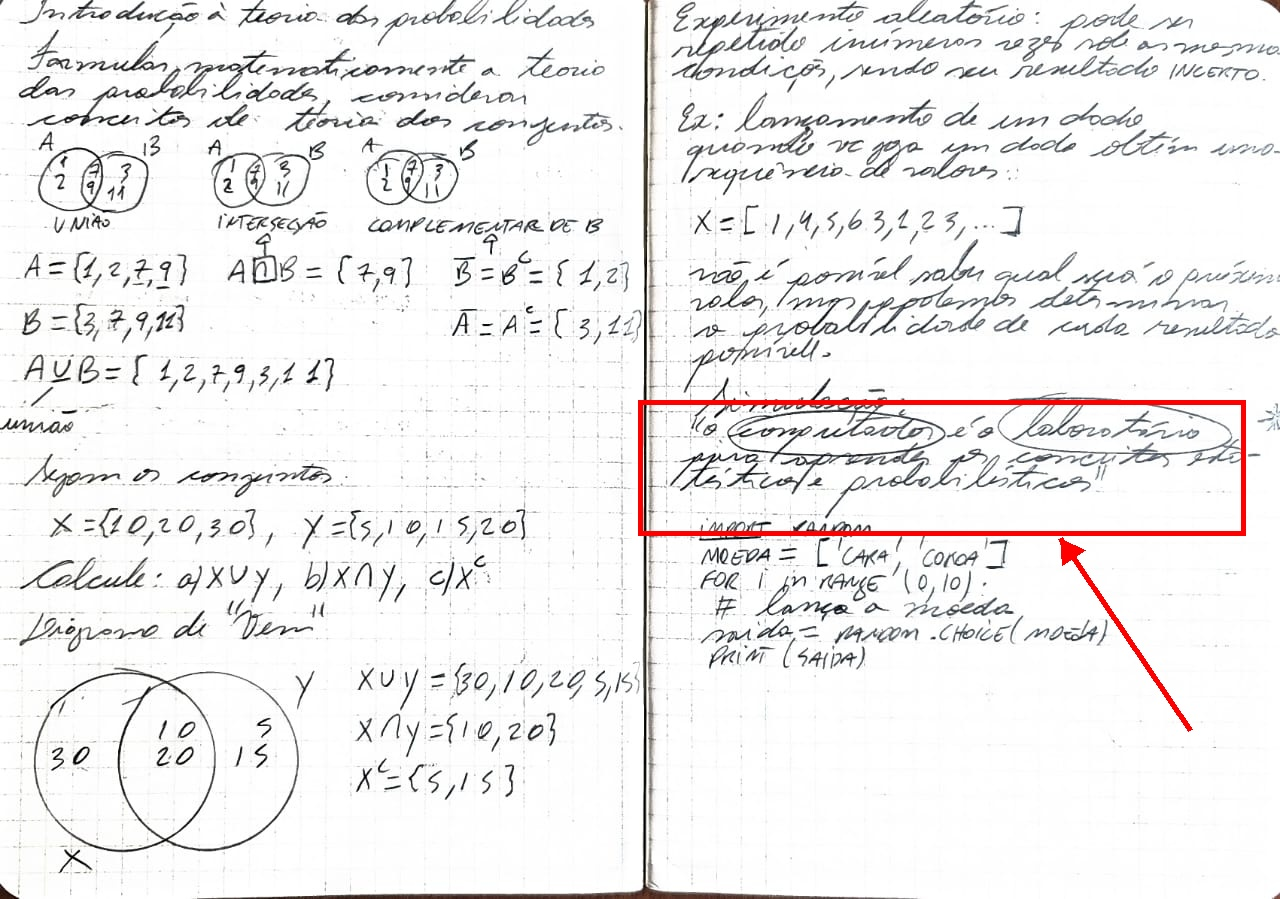
\includegraphics[width=0.7\textwidth]{figuras/cap.1/caderno_quadro.jpg}
  \caption[Anotação de caderno de campo de 28 de julho de 2025]{Anotação do meu caderno de campo de 28 de julho de 2025 durante o curso \textit{Fundamentos de Probabilidade e Estatística para Ciência de Dados} (ICMC-USP, Prof.~Dr. Francisco~A. Rodrigues). O quadro destaca a frase: \enquote{Simulação: `o computador é o laboratório para aprender os conceitos estatísticos e probabilísticos'.} As palavras \enquote{computador} e \enquote{laboratório} estão circuladas.}
  \label{fig:caderno-rodrigues}
\end{figure}

O nível de letramento técnico necessário varia conforme o objeto de estudo: investigações focadas nas práticas de pesquisa em inteligência artificial, como foi meu caso, exigem conhecimento aprofundado. A necessidade de letramento que experimentei encontra eco em debates dentro da própria ciência da computação. \textcite{Wallach2014} formula pergunta que espelha, desde dentro do campo, o que a ecologia das práticas de Stengers permite nomear de fora: poucos cientistas da computação desenvolveriam modelos para analisar dados astronômicos sem envolver astrônomos; por que, então, tantos métodos para analisar dados sociais são desenvolvidos sem o envolvimento de cientistas sociais? A resposta de Wallach é que temos intuições fortes sobre o mundo social, e essas intuições nos fazem crer que compreendemos fenômenos sociais sem precisar de formação específica. Intuição, porém, escapa à descrição como análise. O argumento de Wallach é estrutural: a colaboração precisa ser séria, no modo de criar equipes genuinamente interdisciplinares, em lugar do modo de convocar um cientista social para cada cem cientistas da computação. Nos termos da ecologia das práticas, o que Wallach identifica é que a prática de construção de sistemas que tomam o social como objeto exige, quando levada a sério, o envolvimento de quem conhece esse objeto com seus próprios requisitos, e não apenas como variável a modelar. O diagnóstico converge com o que \textcite{Vicentin_2022_Esboco} formula a partir de Simondon: sem a conexão entre o fazer técnico e o conhecimento sócio-histórico, a tecnologia permanece aquém de sua ética imanente, limitada a reproduzir estruturas existentes em lugar de realizar o potencial transformador que o aprofundamento técnico abre.

O argumento desta compostagem pode agora ser reunido. O momento de que parti produziu fricção, e a fricção revelou que a prática de pesquisa em IA e a da etnografia têm requisitos que não se traduzem por um critério comum. Minha resposta foi habitar essa fricção: buscar letramento técnico suficiente para acompanhar os pesquisadores em seus próprios termos, sem com isso pretender que a diferença entre as práticas se dissolvesse ou que eu me tornasse pesquisadora de computação. Stengers descreve essa aposta com o conceito de \emph{wager}: a aposta de que coletivos com preocupações distintas podem entrar em novas relações simbióticas se souberem aprender uns com os encontros com os outros \parencite[p.~103--104]{stengers2018another}. O letramento foi, nesse sentido, a forma que essa aposta tomou na minha pesquisa, um modo de sustentar o encontro entre práticas com exigências distintas que não se confunde com rendição nem com denúncia, e que transformou a fricção em fermentação.\footnote{O letramento que defendo aqui guarda uma ambiguidade quando passa do meu caso, o da pesquisadora cujo objeto é a própria IA, para a narrativa mais ampla do \emph{AI literacy} dirigida ao usuário leigo de IA generativa. Aprender a usar esses sistemas é exigência legítima de quem quer usá-los com autonomia crítica; a mesma exigência, porém, serve de álibi quando erros estruturais dos sistemas, as alucinações e os vieses que não dependem da perícia de quem usa, são reinterpretados como incompetência do usuário. Reconhecer essa ambiguidade não cancela a exigência do letramento; impede que ela desresponsabilize quem produz os sistemas. Desenvolvo a face técnica desse argumento na seção~\ref{sec:etnografias_ia_mediacao} do capítulo~\ref{capitulo2}, onde distingo o que está nas mãos dos desenvolvedores do que está nas mãos dos usuários.}

\subsection{Compostando a política: ciência como captação de recursos}
\label{subsec:compostagem4}

De todas as compostagens, esta foi talvez a mais imediata, embora tenha sido a última a se formular como tal. Preciso ser franca sobre algo que me acompanhou durante boa parte do trabalho de campo: irritação surda, difícil de formular na época, com o fato de que eu não via a inteligência artificial sendo feita, ao menos como eu imaginava. Eu havia me proposto a fazer uma etnografia de um centro de pesquisa em IA, e os leitores de uma tese como esta esperariam, com razão, saber como a inteligência artificial é produzida. O que eu encontrava, contudo, era outra coisa: eventos de difusão científica, negociações de financiamento, apresentações a parceiros corporativos, disputas por infraestrutura computacional.
A pesquisa em IA parecia acontecer em outro lugar, sempre atrás de uma porta que eu não conseguia abrir, dentro de computadores aos quais eu não tinha acesso, em reuniões técnicas cujo vocabulário eu não dominava. O que eu tinha diante de mim era, como defendo nas compostagens anteriores, a própria construção da inteligência artificial. Eu apenas não a identificava dessa maneira, porque seguia em busca da ciência por trás de toda aquela política.

Assistia a Fábio apresentar o Centro em eventos de difusão e anotava \enquote{divulgação}, em lugar de \enquote{ciência}. Ouvia Cláudio explicar como navegava entre os três potes de recursos e classificava aquilo como \enquote{gestão}, em lugar de \enquote{pesquisa}. Quando Cláudio me descreveu em entrevista como, um mês antes de \textit{deadlines} de conferências, tornava-se impossível conseguir GPU no Centro, reconheci ali o mesmo padrão: eu teria classificado aquilo como \enquote{logística}, em lugar de decisão epistemológica. Na minha primeira visita ao Centro, parei diante da sala de TI sem compreender o que acontecia ali. Anos depois, percebi que aquele desconforto era sintomático de uma separação que eu carregava e que o campo insistia em desfazer. Eu procurava a inteligência artificial dentro dos computadores, nos códigos, nos modelos, e o que encontrava eram pessoas negociando, traduzindo interesses, reconfigurando alianças. A angústia era intelectual e profissional, e me perguntava com frequência como apresentar uma etnografia de um centro de inteligência artificial sem propriamente descrever como a IA é feita.

Essa frustração, contudo, era metodologicamente produtiva. Ela me sinalizava o ponto exato onde minhas categorias analíticas falhavam, onde o arranjo que eu trazia precisava ser reconfigurado. Law argumenta que o \textit{hinterland} de qualquer método se ramifica indefinidamente para além de laboratórios e protocolos, alcançando conhecimento tácito, \textit{software}, habilidades linguísticas, capacidades de gestão, sistemas de transporte e comunicação, escalas salariais, fluxos de financiamento, prioridades de agências de fomento e agendas abertamente políticas e econômicas \parencite[pp.~41--42]{Law2004After}. O que eu observava no \texttt{C4AI} (as sessões de \textit{Design Thinking} que costuravam critérios da USP, \texttt{IBM} e Brasil; a venda da divisão de saúde da \texttt{IBM} que redirecionava linhas de pesquisa; as disputas por GPU que se tornavam decisões epistemológicas; Fábio apresentando em Bluetalks como parte do fazer ciência) era precisamente esse \textit{hinterland} ramificado que métodos convencionais relegam à invisibilidade.

Law descreve \textit{method assemblage} como produção de feixe de relações ramificadas que gera presença, ausência manifesta e \textit{otherness} \parencite[p.~84]{Law2004After}. No meu caso: a presença esperada era a ciência sendo feita (códigos, modelos, experimentos); a ausência manifesta eram as negociações que eu sabia serem necessárias e classificava como \enquote{entorno}; e a \textit{otherness} era precisamente o trabalho de captação de recursos que precisava desaparecer para que a ciência aparecesse como autônoma. Minha frustração era sintoma de que minhas categorias prévias produziam exatamente essa divisão entre presença, ausência e \textit{otherness}. O que o campo me obrigou a fazer foi reconfigurar essas fronteiras: reconhecer que o que eu havia relegado à \textit{otherness} era constitutivo da presença.

A pergunta \enquote{onde está a ciência que esses recursos sustentam?} pressupunha a separação entre ciência e política que o próprio campo tratava de desmentir. Captar recursos, negociar parcerias, justificar investimentos perante agências de fomento e corporações transnacionais é a pesquisa ela mesma. A pergunta não encontrou resposta; perdeu sentido.

A dificuldade em reconhecer aquelas atividades como fazer IA era expressão concreta da alienação técnica discutida anteriormente: a separação entre o que seria estritamente técnico e o que seria entorno da pesquisa reproduz a cisão que impede o amadurecimento da tecnologia. O que o campo me obrigou a compreender, por vias etnográficas, foi que as negociações de financiamento, as disputas por GPU, as apresentações a parceiros corporativos eram parte constitutiva da individuação técnica da IA.

Essa inseparabilidade entre ciência e política era o que o campo me dava a ver quando eu conseguia suspender a distinção prévia. Os próprios projetos de pesquisa do Centro foram definidos, como Fábio me relata, por sessões de \textit{Design Thinking} em que três critérios precisavam se alinhar simultaneamente: a USP teria liderança científica no tema, a \texttt{IBM} teria interesse na temática, e o Brasil teria diferencial internacional. A decisão era uma só, e nela se fundiam avaliação epistêmica, estratégia corporativa e posicionamento geopolítico, sem que houvesse momento científico de escolha de tema seguido de momento político de negociação de recursos.\footnote{Os relatórios internos do \texttt{C4AI} documentam esse processo: o grupo de \textit{Design Thinking} organizou quatro reuniões com mais de 80 pesquisadores, convergindo em cinco desafios. O critério exigia que os resultados fossem estratégicos para o Brasil, relevantes para USP e \texttt{IBM} e com alto potencial de inovação. A partir de 2022, quando a \texttt{IBM} vendeu Watson Health, o Centro decidiu não enfatizar esforços relacionados a saúde; quando o grupo AgriBio conquistou financiamento independente (INCT), tornou-se autossuficiente em relação aos recursos do \texttt{C4AI}. Em ambos os casos, a reconfiguração não separava decisão científica de decisão política.}

Quando a \texttt{IBM} vendeu sua divisão de saúde, o Centro parou de investir diretamente em pesquisa de IA em saúde. Quando a \texttt{IBM} saiu de agronegócio, o mesmo ocorreu. As reorientações de pesquisa se davam como reconfigurações da rede em que agenda científica e interesse corporativo constituíam, desde a origem, um único arranjo, em lugar de imposições externas sobre uma agenda científica autônoma.

Do mesmo modo, quando Fábio apresentava resultados em eventos como as Bluetalks, estava recrutando aliados, fortalecendo a rede, traduzindo interesses de públicos heterogêneos para manter a cadeia de associações que tornava a pesquisa possível. Latour descreve precisamente esse trabalho como constitutivo da prática tecnocientífica: o que se perde ao separá-lo da ciência propriamente dita é justamente o que o torna ciência, ou seja, a capacidade de alistar e manter associados elementos heterogêneos \parencite{Latour2011CienciaEmAcao}. A junção dos termos técnica e ciência em \textit{tecnociência} é exigência empírica, e o campo que eu observava tornava essa exigência particularmente visível.

A agência, nessas reconfigurações, é distribuída pela rede: emerge das associações entre pesquisadores, instituições, infraestruturas, contratos, modelos computacionais e políticas de fomento. Nenhum desses elementos age sozinho ou determina sozinho o curso da pesquisa. Quando o \texttt{C4AI} delega a definição de temas de pesquisa a sessões de \textit{Design Thinking} que costuram simultaneamente critérios da USP, da \texttt{IBM} e do Brasil, a agência dessa decisão reside na associação entre os participantes, e cada reconfiguração da rede redistribui a agência por novas cadeias de translação.

O cenário contemporâneo de investimentos massivos em inteligência artificial (com a concentração de capacidade computacional em poucas corporações, a corrida geopolítica por soberania tecnológica e a crescente dependência de infraestruturas de alto custo) torna essas dinâmicas particularmente visíveis. Resta saber se a pesquisa em IA é caso em que a inseparabilidade entre ciência e política se intensifica a ponto de exigir novos instrumentos analíticos, ou se apenas torna mais difícil ignorar o que Latour já descrevia em outros campos, quando os investimentos eram menores e as redes, menos extensas.

\section{Arremate: etnografias e compostagens}
\label{sec:conclusoes-cap1}

Este capítulo funcionou como laboratório de suas próprias decisões. Começou pela pergunta sobre onde está o laboratório dos pesquisadores de IA do \texttt{C4AI}, e a resposta me exigiu um conjunto de movimentos que o próprio capítulo inscreveu enquanto os realizava: deslocar minha expectativa do laboratório centralizado para o laboratório disperso e portátil, reconhecer a inteligência artificial como ciência em construção em lugar de objeto consolidado, e aceitar que a etnografia de uma rede tecnocientífica desse tipo se faz por composição de materiais heterogêneos, em lugar de descrição linear de um lugar único.

Recapitulo o percurso seção por seção antes de reuni-lo. Abri o capítulo com a pergunta sobre onde está o laboratório dos pesquisadores de inteligência artificial e onde estão os seus cientistas, e parti da fotografia da entrega do primeiro supercomputador à \texttt{OpenAI} em 2016 para situar a infraestrutura computacional como condição de entrada do campo; a resposta deslocou a minha expectativa de um laboratório centralizado para um laboratório disperso e portátil, e firmou a inteligência artificial como ciência em construção, e não como objeto consolidado. Na seção sobre etnografia heterodoxa, articulei a teoria ator-rede de Latour à etnografia de Kofes para sustentar que o método se ensaia enquanto se experimenta, e mostrei que as duas abordagens enfrentam o mesmo problema por vias distintas, a de seguir os actantes e a de deixar-se afetar pelo encontro de campo, o que me autorizou a tomar a própria tese como inscrição tecnocientífica que faz redes ao descrevê-las.

Na seção sobre cortar e costurar redes, tratei o corte como a operação que delimita uma rede que de outro modo se daria a ver como infinita, e reuni cinco modos do corte (Strathern, Barad, Haraway, Costa e Law) para descrever os quatro cortes que cada capítulo da tese faz, cada um pela tríade de Law (presença, ausência manifesta e \textit{otherness}) e legível como \textit{enactment} no sentido de Mol; recuperei ali a etimologia de \textit{contexto} como \textit{contexere}, tecer junto, para fazer trabalhar em português a relacionalidade têxtil que Law nomeia com \textit{hinterland}. Na seção sobre o \textit{patchwork}, desenvolvi a figuração têxtil do método pelo \textit{crazy quilt}, em que a heterogeneidade dos retalhos, a visibilidade das costuras e a recusa de um padrão geral correspondem ponto a ponto ao que a tese precisa fazer ao compor materiais heterogêneos, e diferenciei a minha posição da malha de Ingold, que recusa o corte, para ficar com Strathern e Haraway, para quem cortar é condição da descrição.

Na seção sobre existências parciais, parti do princípio de simetria de Latour e o desdobrei até as existências parciais, organizando os conceitos da seção (híbrido, quase-máquina, agência distribuída, conexão parcial, fazer-com) por uma grade de três planos, substância, propriedade e efeito-relação, que converge para o eixo de que a relação constitui; descrevi os sistemas de inteligência artificial generativa como máquinas e, na leitura que faço de Latour, também como quase-máquinas no plano do efeito-relação, reconheci o \texttt{claude} como objeto múltiplo, e tratei os instrumentos de inscrição da tese como actantes que se compõem comigo. Na subseção sobre por que fazer parentesco com este problema, sustentei que o meu fazer-com a inteligência artificial generativa é escolha metodológica deliberada de ficar com um companheiro problemático, e documentei essa escolha com a sequência de três capturas de tela de uma conversa de revisão com o \texttt{claude}, em que a régua estilística do modelo é contestada, recua e se reformula, e a agência epistêmica se redistribui turno a turno. Na passagem cosmotécnica, situei o fazer-com entre uma antropóloga brasileira e um modelo treinado predominantemente em dados anglófonos como gesto cosmotécnico particular, no sentido de Hui.

Na subseção em que defini a tecno-etnografia, distingui-a da etnografia digital de Pink, Horst e Postill por uma inflexão, a de fazer a pesquisa não só \textit{sobre}, mas \textit{com} a inteligência artificial generativa, tomada ao mesmo tempo como objeto e como dado, com auditabilidade pública das técnicas nos repositórios do \texttt{GitHub} como contraparte material e ética desse compromisso; e produzi, como demonstração, seis inscrições do próprio capítulo, três sincrônicas que respondem ao que se liga a quê na minha escrita e três diacrônicas que respondem a quando cada conceito entra, persiste e migra, das quais retive que a minha costura argumentativa ainda se apoia em palavras genéricas a teorizar e que a conexão entre as ciências sociais e o par humano-máquina-método é a \textit{otherness} que ainda preciso fazer trabalhar. Na seção sobre compostagens, nomeei quatro fermentações de materiais que o desenho inicial da pesquisa mantinha separados, a do método (a regra de estudar a ciência em construção com a dispersão da pesquisa em inteligência artificial), a da teoria (a simetria que se decompôs em existências parciais no próprio trabalho de campo), a do letramento (a minha formação em ciências sociais com o letramento técnico que o campo me exigiu, depois de pesquisadores da computação contestarem os conceitos de Pasquinelli e Crawford que levei a uma aula) e a da política (a separação prévia entre ciência e política desfeita pela evidência de que a pesquisa no \texttt{C4AI} é, ao mesmo tempo, decisão epistêmica e captação de recursos).

Três gestos analíticos se desdobraram a partir dessa pergunta inicial. O primeiro foi nomear cortes, ou seja, os gestos de delimitação que tornam descritível uma rede que se desdobra indefinidamente.
A subseção \enquote{Cortando redes} convocou o corte de Strathern e conceitos vizinhos de Barad, Haraway, Costa e Law para descrever como cada capítulo desta tese faz um corte específico: reflexivo no capítulo~\ref{capitulo1}, teórico no capítulo~\ref{capitulo2}, pela extensão no capítulo~\ref{capitulo3} e pela densidade no capítulo~\ref{capitulo4}. Os quatro cortes funcionam como \textit{enactments} no sentido praxiográfico que Mol e Law desenvolvem, e os quatro capítulos performam o \texttt{C4AI} como quatro objetos etnográficos que se atravessam sem se subsumir uns aos outros.

O segundo gesto foi descrever o fazer-com a inteligência artificial generativa que minha tese assume como dado etnográfico, em lugar de recurso técnico secundário. A seção \enquote{Existências parciais} desdobrou um movimento teórico interno à obra de Latour, do princípio de simetria como ponto de partida à formulação das existências parciais como descrição mais precisa do que o campo me apresentava. Esse movimento gerou três contribuições. A noção de quase-máquina, que tomo de Latour como leitura e não como definição, me permitiu descrever esses sistemas, que são máquinas, também como entidades abertas e parcialmente conectadas, que escapam à partição entre humano e não humano. A noção de agência distribuída descreveu o mecanismo pelo qual essas existências parciais agem juntas, redistribuindo a responsabilidade pela ação por cadeias de translação. A multiplicidade ontológica de Law me permitiu reconhecer o \texttt{claude} como objeto múltiplo (em treinamento, em \textit{deployment}, em auditoria, em uso), e cada Claude existe como fazer-com situado com quem o aciona, em lugar de objeto singular acessível a todos.

O terceiro gesto foi figurar as transformações recíprocas que tornaram minha pesquisa possível. A seção \enquote{Compostagens} nomeou quatro misturas específicas de materiais heterogêneos que precisaram fermentar juntos para que a descrição se tornasse possível: a regra latouriana de estudar a ciência em construção fermentando com a dispersão característica da pesquisa em IA; a simetria metodológica fermentando com a especificidade da inteligência artificial generativa para gerar existências parciais; minha formação em ciências sociais fermentando com o letramento técnico que o campo me exigiu; e a separação prévia entre ciência e política fermentando com a evidência empírica de que a pesquisa em IA, no \texttt{C4AI}, é simultaneamente decisão epistêmica e captação de recursos. Cada compostagem inscreve um momento em que a descrição etnográfica exigiu decompor partições prévias e tolerar a fermentação de materiais que o desenho inicial da pesquisa mantinha separados.

O que sustenta este capítulo é, antes de teórico, etnográfico, e ele me deixou com uma questão que carrego pela tese inteira e que prefiro não fechar aqui. Penso e construo o argumento por uma figuração têxtil, em que o trabalho de pesquisa se faz de fios, tramas, costuras, nós e cortes, e ao mesmo tempo inscrevo o seu percurso em diagramas, gráficos e textos-mapa que disponho ao longo do capítulo para dar a ver, numa superfície plana, o que de outro modo se perderia na dispersão. São duas figurações que constituem esta tese, e que vim a reconhecer como figurações topológicas, no sentido em que a própria teoria ator-rede é topológica: a rede de \textcite{latour1996clarifications}, que retomei na subseção~\ref{subsec:cortando-redes}, tem caráter fibroso, feito de fios e laços tecidos, e a força dela vem do tecer cuidadoso de laços fracos. A rede de Latour é, ela própria, um tecido, e por isso rede e trama não são figurações opostas, e sim homólogas sem serem homogêneas: as duas são feitas de fios e nós, mas de materiais distintos e em formas distintas de apresentação, a rede que recruta e vence em Latour e a trama que oferece e fica-com em Haraway. É essa homologia que sustenta a passagem deste capítulo aos capítulos~\ref{capitulo3} e~\ref{capitulo4}, em que faço, corto e sigo redes, porque a rede que descrevo no campo e a trama com que escrevo a tese são o mesmo gesto têxtil em fios de matéria diferente.

A mesma topologia, porém, separa duas ordens de cognição. Pensar em rede é pensar topologicamente, em nós de tantas dimensões quantas forem as suas conexões, o que nenhuma superfície plana comporta; mostrar uma rede é fácil, basta conectar os nós numa superfície de duas dimensões. A figuração têxtil, com que penso, pertence à primeira ordem, e os textos-mapa, com que inscrevo, à segunda, e por isso a têxtil não aparece nas figuras: ela é o pensamento que produz as figuras, e não uma das figuras. A compostagem que desdobrei na seção sobre as fermentações é, do mesmo modo, figuração do pensamento, e não da inscrição, porque fermentar materiais heterogêneos para que se transformem uns nos outros é um modo de pensar com eles no tempo, da mesma ordem do tecer, e tampouco se deixa mostrar numa superfície: o que um diagrama exibiria seria o resultado da mistura, não o fermentar que a fez. Demorei a reconhecer que a figuração têxtil não podia ser desenhada, e que essa impossibilidade não era falha minha nem da figura, e sim a natureza de cada uma. Um mapa mostra nós e conexões, isto é, as coisas já postas em relação; não mostra o relacionar que as pôs assim, e é esse relacionar que a trama pensa. A relação, como sustento desde a subseção~\ref{subsec:cortando-redes} a partir de Strathern, nunca está dada, e se refaz a cada corte e a cada costura que escolho fazer, e a superfície da inscrição só recebe o resultado da relação, não a relação em ato.

Habito, nesse ponto, uma tensão que não chega a ser contradição, e é dela que esta tese se faz: pratico na escrita um modo de pensamento que não cabe na superfície em que inscrevo os textos-mapa, e os dois coexistem sem que um se reduza ao outro. A coexistência das duas figurações, em lugar da escolha entre elas, é parte do que proponho, e as duas mexem com sentidos distintos, o tato e o tempo do raciocínio que se tece, e a visão que apreende de uma só vez a superfície plana. Deixo a questão aberta para os capítulos seguintes, sem a pretensão de resolvê-la: se a figuração têxtil é um modo de pensar, e se o que reúne as coisas é uma relação que nunca está dada, como se pensa por tramas, como se mostra esse pensar numa superfície que só recebe o que já foi tecido, e o que acontece quando ponho em questão a própria diferença entre tecer um argumento e mapeá-lo.
O método se ensaiou enquanto se experimentava, conforme a orientação de \textcite{Kofes2015Maconaria}, e os conceitos que convoquei foram chamados pelo que o campo exigia. Esse percurso me autoriza um gesto que executei de modo recursivo neste capítulo~\ref{capitulo1}: aplicar à própria escrita da tese o tratamento que aplico aos pesquisadores que descrevo. A subseção \enquote{Tecnoetnografia} converteu o texto deste capítulo em grafo de co-ocorrências e leu suas comunidades como tópicos latentes, inscrevendo as costuras conseguidas e as fissuras pendentes. A subseção \enquote{Por que fazer parentesco com este problema?} documentou em sequência de capturas de tela uma cena de fazer-com o \texttt{claude} durante a revisão deste mesmo capítulo. Em ambos os casos, minha tese funciona como inscrição tecnocientífica que se deixa medir pelos mesmos instrumentos com que se compromete a medir o \texttt{C4AI}, e a reflexividade metodológica assume a forma de gesto recursivo, em lugar de declaração externa sobre a relação entre quem pesquisa e objeto.

O que este capítulo deixou em aberto é o desdobramento da tecno-etnografia nas três tramas que organizam os capítulos seguintes. Cada uma delas retoma, em escala e materialidade próprias, os três gestos analíticos que este capítulo desenvolveu sobre a sua própria escrita: o corte que delimita a rede para torná-la descritível, a compostagem que põe materiais heterogêneos a fermentar juntos, e a descrição das existências parciais que se compõem na pesquisa. O que o capítulo~\ref{capitulo1} entrega aos capítulos etnográficos é a consciência de que a figuração com que se descreve a tecnociência é parte do que se descreve, e que essa figuração precisa ser assumida em vez de naturalizada, e não um sumário do que cada um fará.

Esse legado tem consequências diretas para o que esta tese pode descrever nos capítulos seguintes. Se eu deixasse o trabalho sobre as figurações implícito, descreveria o \texttt{C4AI} no capítulo~\ref{capitulo3} e o \texttt{Spira} no capítulo~\ref{capitulo4} usando, sem perceber, o vocabulário militar-industrial em que Latour formulou a tecnociência, isto é, alistar aliados, recrutar para vencer, mobilizar provas de força, sustentar a máquina de guerra das publicações e dos consórcios. Esse vocabulário não é falso, é figuração específica, e está admitida pelo próprio Latour como mudança de metáforas que contaminou o trabalho descritivo, conforme retomo no capítulo~\ref{capitulo2}. O que faço neste capítulo~\ref{capitulo1}, e adenso no próximo, é abrir o espaço para descrições da tecnociência em outros vocabulários, isto é, descrições que mobilizam costuras de retalho com Strathern, compostagens e tornar-se-com com Haraway, aliar e oferecer com Stengers, e ficar com o problema sem a pretensão de resolvê-lo. As três tramas seguintes, somadas a este capítulo~\ref{capitulo1} que se ofereceu como laboratório de suas próprias decisões, compõem o que esta tese chama de tecno-etnografia, e ocupam, cada uma a seu modo, esse espaço aberto.
\chapter{Metáforas, figurações e alianças: revisão da literatura}
\label{capitulo2}
[atualização 27 de junho]
\epigrafe{%
Seja qual for a tática, é fácil perceber a estratégia geral: faça tudo o que for necessário com a literatura anterior para torná-la o mais útil possível à tese que você vai defender. As regras são bastante simples: enfraqueça os inimigos; paralise os que não puder enfraquecer [\ldots]; ajude os aliados se eles forem atacados [\ldots]. De fato, são regras simples: são as regras dos velhos políticos.}%
{Bruno Latour, \textit{Ciência em ação: como seguir cientistas e engenheiros sociedade afora}, 2011, p.~55}

\begin{figure}[htbp]
  \centering
  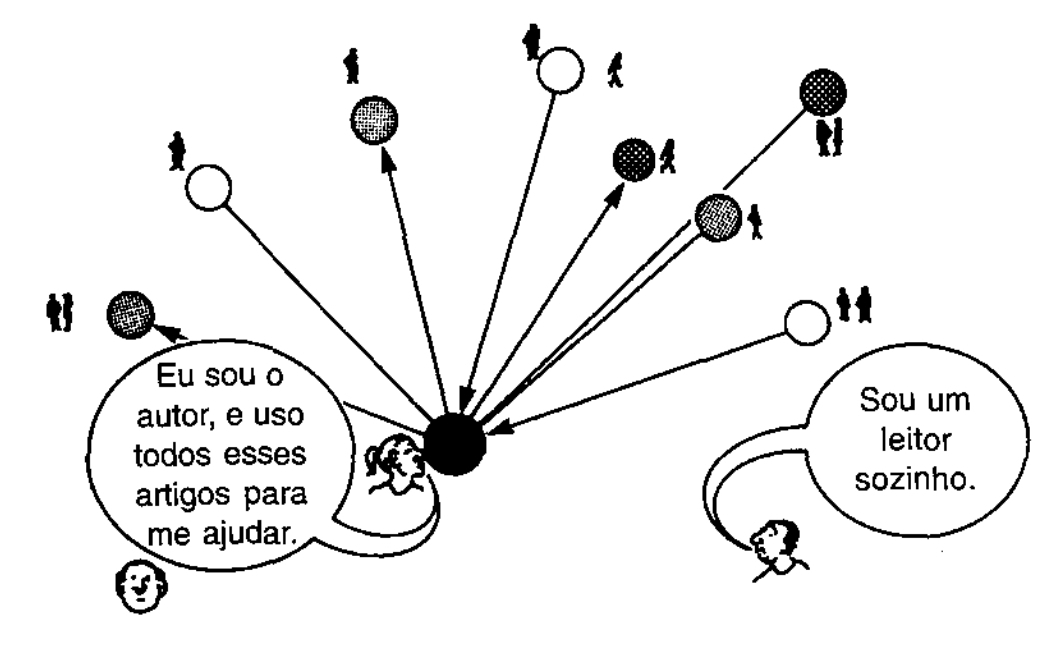
\includegraphics[width=0.6\linewidth]{figuras/cap.2/latour.jpg}
  \caption[O autor cercado de aliados e o leitor sozinho]{O autor cercado de aliados e o leitor sozinho. Figura~1.3 de \textit{Ciência em Ação}.}
  \label{fig:latour_aliados}
  \fonte{\textcite[p.~56]{Latour2011CienciaEmAcao}.}
\end{figure}

\begin{figure}[htbp]
  \centering
  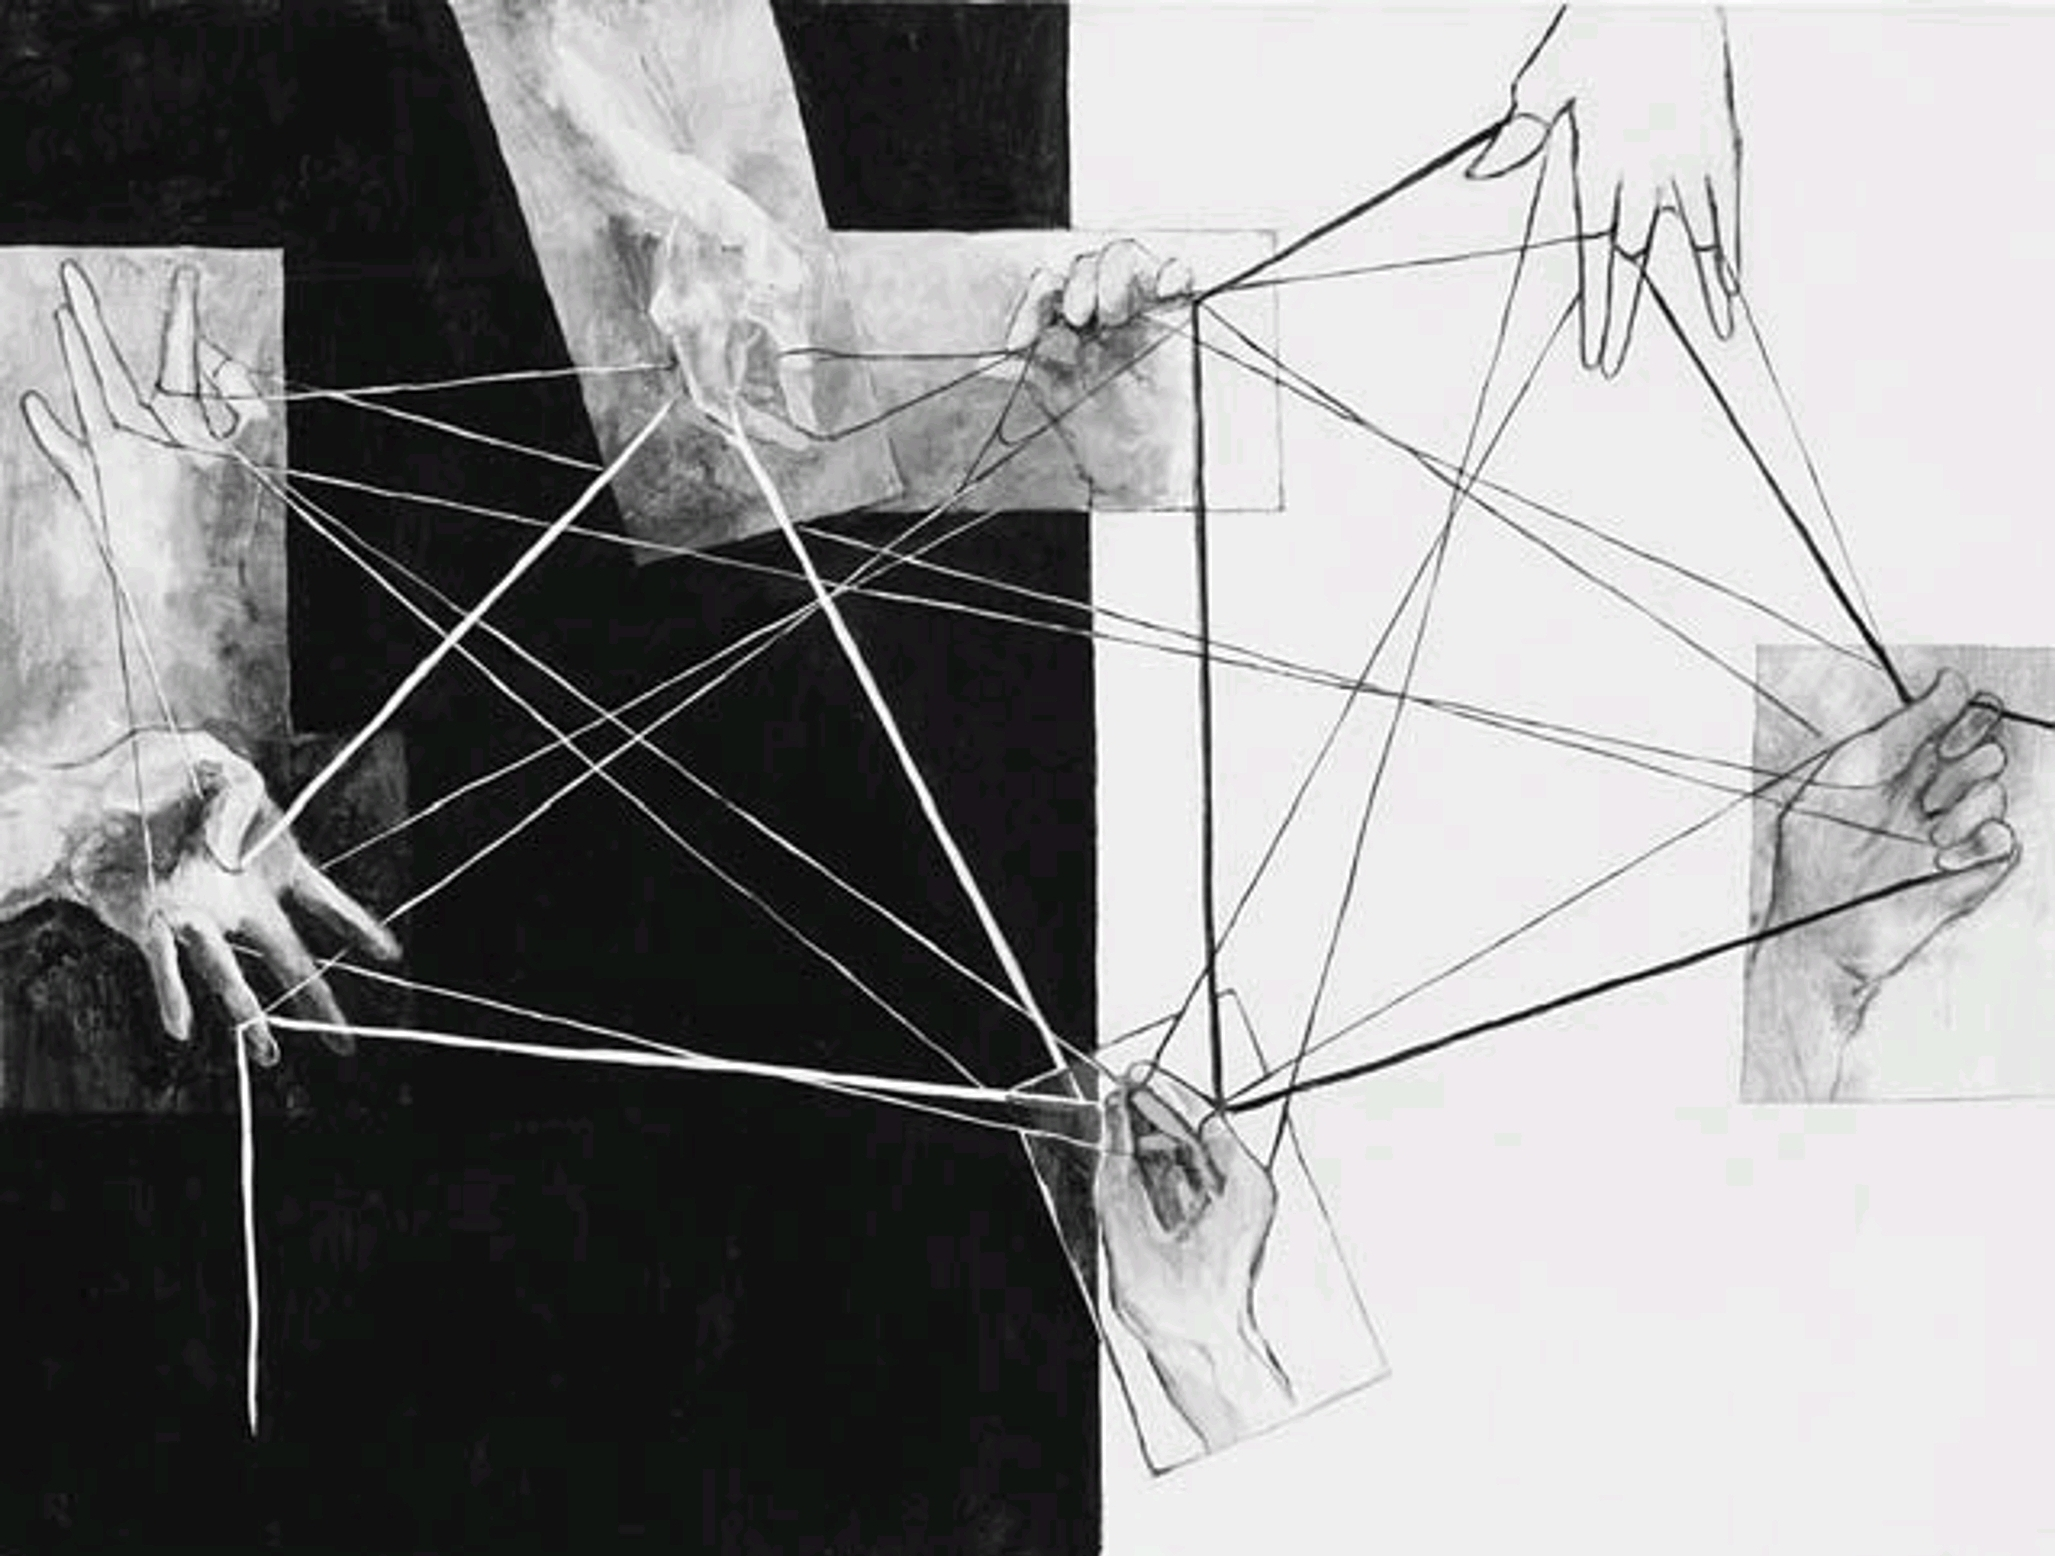
\includegraphics[width=0.6\linewidth]{figuras/cap.2/haraway.jpg}
  \caption[\textit{Cat's Cradle / String Theory}, de Baila Goldenthal]{\textit{Cat's Cradle / String Theory}, de Baila Goldenthal, 2008. Óleo sobre tela, 36~$\times$~48~pol.}
  \label{fig:goldenthal_cats_cradle}
  \fonte{\textcite[p.~35]{Haraway2016Staying}. Cortesia de Maurya Simon e Tamara Ambroson.}
\end{figure}

\epigrafe{%
Importa quais pensamentos pensam pensamentos. Importa quais conhecimentos conhece conhecimentos. importa quais relações relacionam relações. Importa quais mundos mundificam mundos. Importa quais estórias contam estórias. As pinturas de Baila Goldenthal dão um testemunho eloquente da importância dessas matérias.}%
{Donna Haraway, \textit{Ficar com o problema: fazer parentesco no Chthuluceno.}, 2016, p.~69}%

\section{}

Neste capítulo~\ref{capitulo2} retomo o conceito de tecnoetnografia que apresentei no capítulo~\ref{capitulo1}. A tecno-etnografia, conforme defini no capítulo anterior, é um conceito que surge da indissociabilidade entre escrita, análise e técnicas que desenvolvi nesta pesquisa \textit{sobre} e \textit{com} inteligência artificial, e desdobra-se em quatro capítulos, ou quatro tramas --- o capítulo~\ref{capitulo1} apresenta a tecno-etnografia como conceito e prática \textit{junto com}, \textit{junto a} e \textit{sobre} a inteligência artificial para inscrever e descrever as redes tecnocientíficas e sociotécnicas desta tese. O capítulo~\ref{capitulo3} desdobra a tecno-etnografia sobre o \texttt{C4AI} como rede em que \texttt{USP}, \texttt{FAPESP} e \texttt{IBM} são nós de uma trama sociotécnica que atravessa mais de um século de história, e o capítulo~\ref{capitulo4} desdobra-a a partir da investigação de um sistema de inteligência artificial, o \texttt{Spira}, também \textit{junto a} inteligência artificial.

% [NOTA DE REVISÃO 1] Frase final do parágrafo realinhada à formulação revisada nos capítulos 0, 1 e 3: removido "mostra apenas a forma", que rebaixava o mapa a exibição passiva; o mapa também põe em relação, em plano próprio, e nenhum dos dois planos se reduz ao outro. Corrigido de passagem o "que as teço" (redundância pronominal) para "que teço". O restante do parágrafo permanece intacto.
Situo agora sobre o que se trata este capítulo~\ref{capitulo2}. Faço uma revisão da literatura em duas linhas de análise, a análise lexicométrica das figurações na obra de Latour e de Latour e Woolgar e a análise bibliométrica do campo brasileiro e internacional de estudos envolvendo a inteligência artificial nas ciências humanas e sociais, e entre as duas recolho as leituras que cada problema empírico do meu campo evocou, dos estudos da ciência e da tecnologia às genealogias críticas do poder tecnocientífico. O mapa da Figura~\ref{fig:mapa-cap2} dá a ver a estrutura geral deste capítulo: os fundamentos que o sustentam, as seções e subseções com os autores e achados que as ocupam, as relações que as ligam, e o arremate que mantém em aberto a tensão entre alistar aliados com Latour, tecer tramas com Haraway, e propor alianças com Stengers. O diagrama pertence ao registro da inscrição, e põe em uma superfície bidimensional, de uma só vez, aquilo que o texto só pode percorrer em sequência, página após página. Reúno ainda, na linha do tempo da Figura~\ref{fig:linha-tempo-cap2}, as tradições teóricas que recolho ao longo do capítulo e o ponto em que esta tese se insere entre elas, dispostas pela data de seus marcos. Reencontro aqui a tensão que abro na Apresentação e desdobro no capítulo~\ref{capitulo1}: a urdidura, a trama e as texturas como figuras do pensamento que teço ao longo dos capítulos, no tempo e na espessura da escrita, e o mapa como o plano em que essas mesmas relações se inscrevem e fazem aparecer ligações que a leitura sequencial não alcança. Os dois planos põem em relação, cada um à sua maneira, e nenhum se reduz ao outro.

\begin{figure}[htbp]
  \centering
  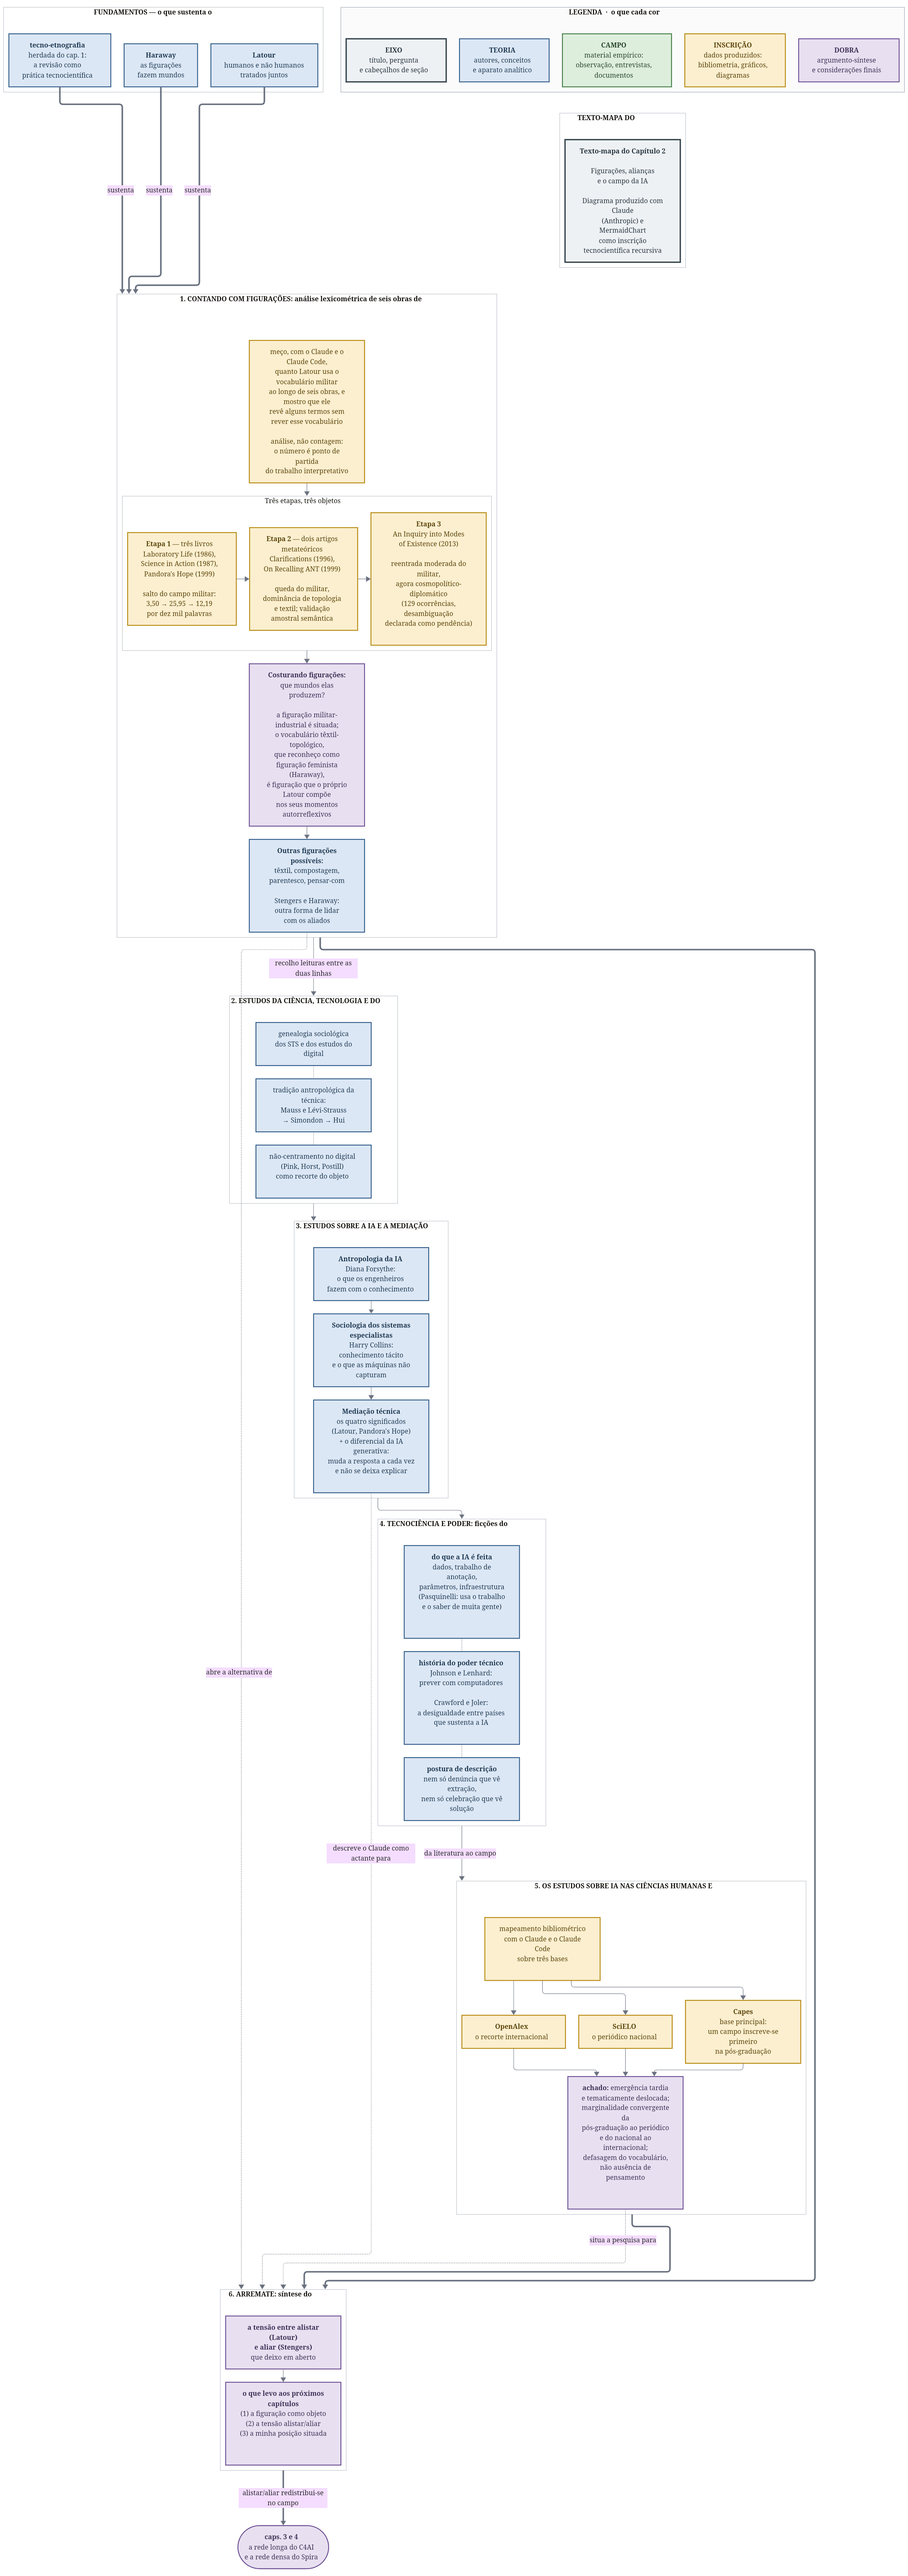
\includegraphics[width=0.3\linewidth,keepaspectratio]{figuras/cap.2/diagramas/mapa-capitulo2.png}
  \caption[Mapa do capítulo~\ref{capitulo2}]{\textbf{Mapa do capítulo~\ref{capitulo2}: a análise lexicométrica, as leituras do campo e o mapeamento bibliométrico.} Este mapa situa o leitor no percurso do capítulo, ao dar a ver em uma superfície plana as suas seções e subseções, os autores e achados que as ocupam, e as relações que as ligam, com os fundamentos que as sustentam na base: a ideia de Haraway de que as figurações fazem mundos, o tratamento de humanos e não humanos em pé de igualdade que recolho de Latour, e a tecno-etnografia que herdei do capítulo~\ref{capitulo1}. A primeira seção é a análise lexicométrica que desenvolvi com o \texttt{claude} e o \texttt{claude code}, em que meço quanto Latour usa o vocabulário militar ao longo de seis obras e mostro que ele revê alguns dos seus termos sem rever esse vocabulário, e que se desdobra em três subseções, sobre o corpus estendido dos dois artigos metateóricos, sobre a figuração em \emph{An Inquiry into Modes of Existence}, e sobre as figurações que produzem outros mundos (a têxtil, a compostagem, o parentesco e o pensar-com, com Stengers e Haraway). A segunda seção situa a pesquisa nos estudos da ciência, da tecnologia e do digital, com a tradição antropológica da técnica de Mauss e Lévi-Strauss a Simondon e Hui. A terceira trata da inteligência artificial e da mediação técnica, em três subseções, sobre a antropologia de Diana Forsythe, sobre a sociologia dos sistemas especialistas de Harry Collins, e sobre os quatro significados de mediação que Latour assenta em \emph{A Esperança de Pandora} e aquilo que a inteligência artificial generativa tem de diferente. A quarta seção descreve do que a inteligência artificial é feita, dos dados e do trabalho de anotação aos parâmetros e à infraestrutura, com Pasquinelli, Johnson e Lenhard, Crawford e Joler, e a desigualdade entre países que sustenta esses sistemas. A quinta mapeia o campo brasileiro de estudos em inteligência artificial nas ciências humanas, a partir das bases da \texttt{Capes} e do \texttt{SciELO} e do contexto internacional do \texttt{OpenAlex}, e mostra um campo recente em que a antropologia ainda comparece pouco. O arremate mantém em aberto a tensão entre alistar, com Latour, e aliar, com Stengers, e leva aos capítulos seguintes três coisas que retomo adiante, a figuração como objeto, essa tensão e a minha posição situada. A inscrição é, ela mesma, parte do que descreve, e funciona, no sentido de \textcite{Latour1986Visualization}, como móvel imutável que reúne em uma só superfície o que o texto desdobra ao longo de dezenas de páginas. Diagrama disponível em versão interativa em: \url{https://mermaid.ai/d/b4a7d089-3a37-4ab6-8e45-fc4ecca9e22f}}
  \label{fig:mapa-cap2}
\end{figure}

\begin{figure}[htbp]
  \centering
  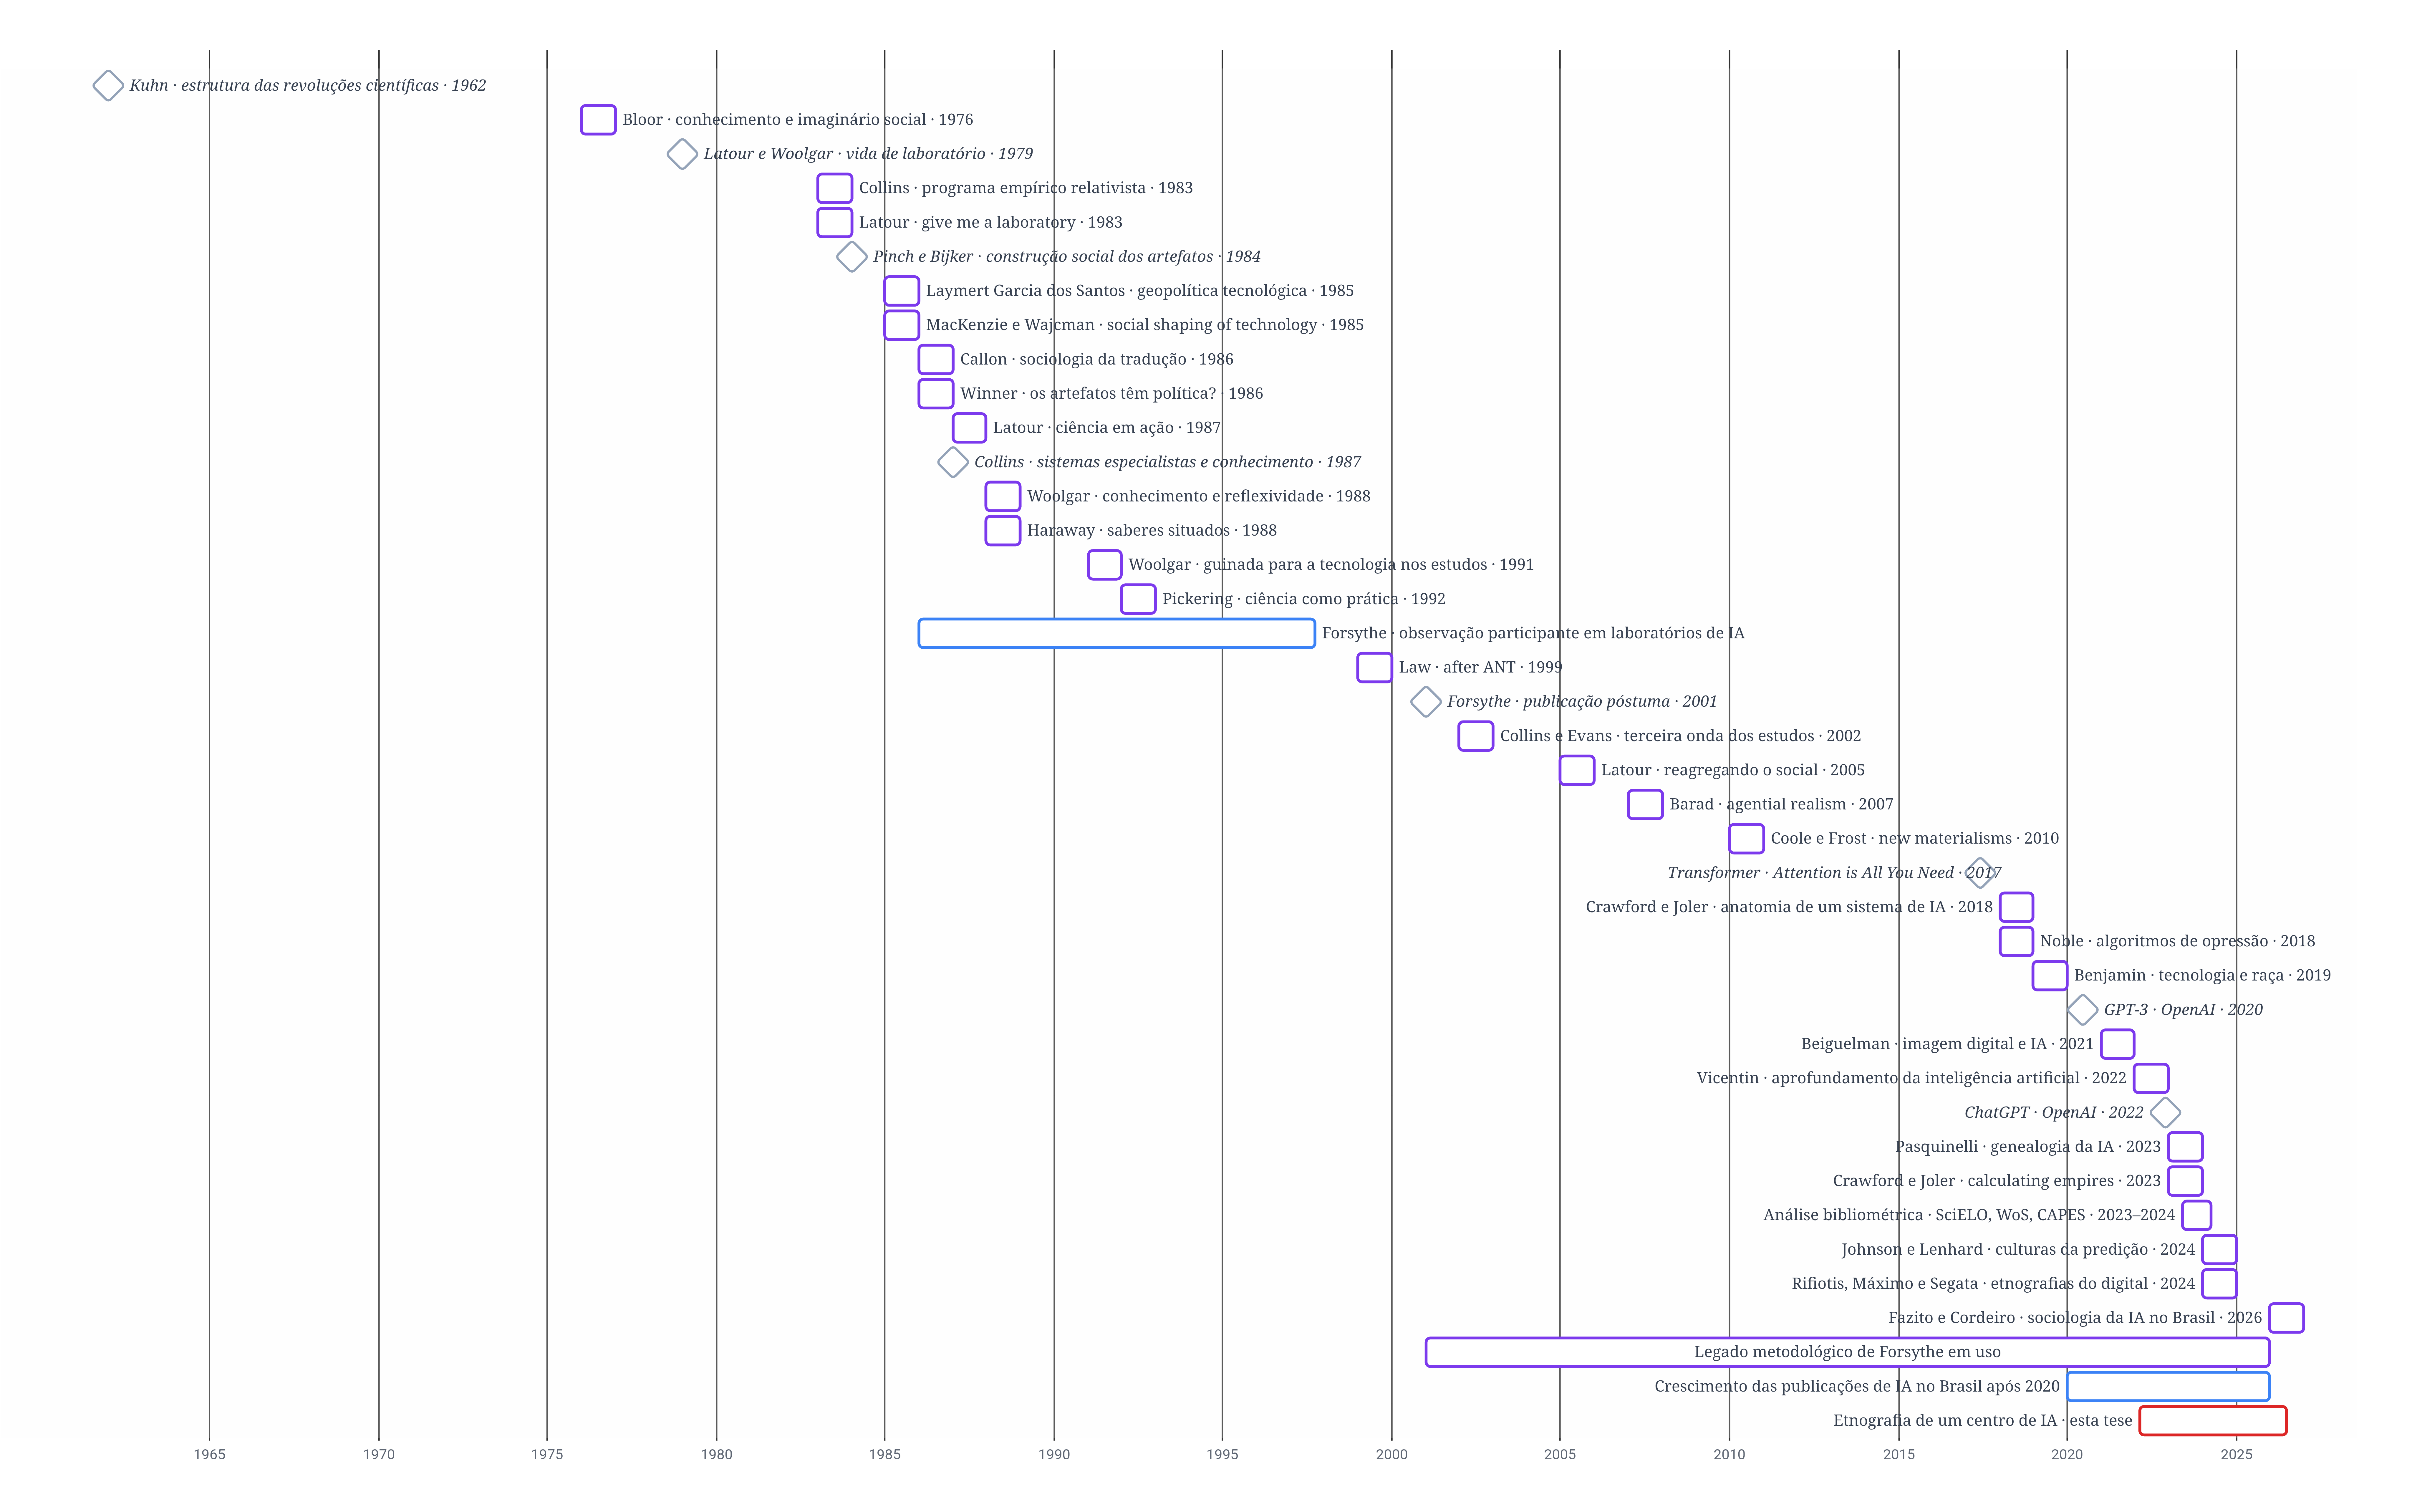
\includegraphics[width=0.85\linewidth,keepaspectratio]{figuras/cap.2/diagramas/linha-tempo-capitulo2.png}
  \caption[Linha do tempo do capítulo~\ref{capitulo2}]{\textbf{Linha do tempo do capítulo~\ref{capitulo2}: as tradições teóricas que recolho e o ponto em que esta tese se insere.} Esta linha do tempo dá a ver, em uma superfície plana, as obras das tradições de pesquisa que recolho neste capítulo, dispostas em sequência pela data de seus marcos, e pertence ao registro da inscrição, no sentido de \textcite{Latour1986Visualization}. O percurso vai da sociologia do conhecimento científico, de \textcite{Kuhn2012Structure} e \textcite{Bloor2009Conhecimento}, à construção social da tecnologia, aos estudos de laboratório e à teoria ator-rede, de \textcite{Latour1997VidaLaboratorio} a \textcite{Latour2007Reassembling}, aos novos materialismos de \textcite{Haraway1991Situated} a \textcite{Coole2010NewMaterialisms}, às etnografias de inteligência artificial de \textcite{Collins2012Expert} e \textcite{Forsythe2001}, às genealogias críticas do poder tecnológico de \textcite{Crawford2018Anatomy} a \textcite{JohnsonLenhard2024}, e ao campo emergente no Brasil, de \textcite{Santos_2022_SociologiaNaoAutocratica} e \textcite{Vicentin_2022_Esboco} a \textcite{Rifiotis2024Etnografias} e \textcite{FazitoCordeiro2026Sociologia}. Três marcos da inteligência artificial generativa atravessam essa produção e situam o leitor quanto ao momento em que a tecnologia que observo em campo emerge: o artigo do \textit{Transformer} em 2017, o \texttt{GPT-3} em 2020 e o \texttt{ChatGPT} em 2022. As duas barras em vermelho marcam onde esta tese se insere: no prolongamento da construção social da tecnologia e como etnografia de um centro de inteligência artificial, entre 2022 e 2026. Diagrama disponível em versão interativa no \texttt{MermaidChart}\footnote{Versão interativa do diagrama disponível em: \url{https://mermaid.ai/d/a7b611c1-a522-41da-9603-0a8be61de483}. Acesso em: \today.}, em que cada obra que o texto percorre em sequência se dispõe ao lado das demais em uma só superfície.}
  \label{fig:linha-tempo-cap2}
\end{figure}

A trama tecnoetnográfica deste capítulo se desdobra em duas linhas onde o conceito de tecno-etnografia é tensionado por meio de suas práticas. A primeira é a análise das metáforas e figurações na obra de Bruno Latour, desenvolvida com o \texttt{claude} e o \texttt{claude code}\footnote{O \texttt{claude} e o \texttt{claude code} são dois produtos da empresa \texttt{Anthropic} que dão acesso ao mesmo modelo de linguagem por interfaces distintas. O \texttt{claude} é a interface de conversação, em janela de \emph{chat} acessível pelo navegador ou por aplicativo, em que a interação se dá por texto, e é o ambiente em que fiz a maior parte da escrita e da discussão dos argumentos desta tese. O \texttt{claude code} é a interface de linha de comando, executada no terminal do computador, em que o modelo tem acesso direto ao sistema de arquivos e pode ler, escrever e executar \emph{scripts}, rodar programas em \texttt{Python} e versionar repositórios sem que eu precise copiar trechos de código entre janelas. As duas linhas de análise deste capítulo recorreram às duas interfaces conforme a tarefa: o processamento de arquivos extensos e a execução repetida de \emph{scripts} foram feitas no \texttt{claude code}, e a discussão dos resultados e a redação combinaram as duas. Sempre que nomeio uma delas em específico ao longo da tese, a escolha registra qual ambiente técnico mediou a tarefa descrita.} a partir de seis livros e artigos publicados entre 1986 e 2013.\footnote{O repositório com os textos normalizados, o catálogo de termos, os \emph{scripts} de extração e contagem em \texttt{Python}, as planilhas de validação e os \emph{outputs} de cada etapa está disponível em \url{github.com/julianehelanski/analise-figuracoes-latour}. Os PDFs das obras de Latour ficam fora do repositório por razões de direitos autorais.} A segunda é o mapeamento da emergência do campo brasileiro de estudos em inteligência artificial nas ciências humanas e sociais, realizado por análise bibliométrica das plataformas \texttt{SciELO} e \texttt{Capes} com o \texttt{claude} e o \texttt{claude code}, com tratamento e visualização de dados em \texttt{Python} no ambiente de programação para análise de dados \texttt{Spyder/Anaconda}.\footnote{O repositório com todos os dados dessa analise está disponível em \url{https://github.com/julianehelanski/analise_bibliometrica_ia_ciencias_humanas}.}
        
Ao disponibilizar publicamente os repositórios do \texttt{GitHub} com os \emph{scripts}, os catálogos, as planilhas de validação e os \emph{outputs} de cada etapa de análise, incluo essa prática comum da ciência de dados e da computação\footnote{O repositório do \texttt{GitHub} permite armazenar e publicar os códigos, os \textit{scripts}, um tipo específico de código criado para automatizar tarefas repetitivas, e os dados utilizados em um estudo, e retornar a qualquer versão anterior do projeto. A publicação desses arquivos permite que outras pesquisadoras verifiquem os resultados e reproduzam a análise.} também como uma prática tecnoetnográfica. A análise em linguagem de programação \texttt{Python}, a automatização da análise textual, as buscas padronizadas nas plataformas de indexação bibliográfica e as sessões recursivas com o \texttt{claude} e o \texttt{claude code} são técnicas em sentido estrito, e são técnicas que podem ser reexecutadas, contestadas ou refinadas a partir dos repositórios públicos. Essas técnicas são parte da pesquisa e do trabalho relacional e situado que transforma os meios, os modos e os resultados que a pesquisa alcança.

O mapeamento bibliométrico que realizei tem por base principal o Catálogo de Teses e Dissertações da \texttt{Capes}, complementado por uma sondagem na biblioteca eletrônica \texttt{SciELO} e pela comparação com a base internacional \texttt{OpenAlex}. Tomei o Catálogo da \texttt{Capes} como base porque o que me interessa é o momento de formação de um campo nas ciências humanas e sociais brasileiras, que se inscreve primeiro na pós-graduação, na tese e na dissertação, antes de chegar ao artigo publicado em periódico. A \texttt{SciELO} e o \texttt{OpenAlex} situam esse campo brasileiro emergente diante da produção em periódico, nacional e internacional. A seção~\ref{sec:emergencia_campo_brasileiro} apresenta esse mapeamento e detalha a escolha das bases, os protocolos de classificação que adotei e os resultados a que cheguei. 

A seção~\ref{sec:analise_lexicometrica} apresenta a análise das metáforas e figurações em Latour, e em Latour e Woolgar, em três etapas: a etapa~1 processou três livros (\emph{Laboratory Life}, de Latour e Woolgar, 1986, \emph{Science in Action} 1987, \emph{Pandora's Hope} 1999); a etapa~2 estendeu a análise a dois artigos metateóricos (\emph{Clarifications} 1996, \emph{On Recalling ANT} 1999);  a etapa~3 processou \emph{An Inquiry into Modes of Existence} (2013). Chamo metateóricos os dois textos da etapa~2 porque nenhum deles descreve um caso, como fazem os três livros da etapa~1, e ambos tomam por objeto a própria teoria ator-rede, que revisam e esclarecem.\footnote{\emph{On Recalling ANT} é um capítulo da coletânea \textit{Actor Network Theory and After}, organizada por John Law e John Hassard \parencite{LawHassard1999ANTAfter}. \emph{Clarifications} circula como \emph{working paper} sem paginação editorial estável, e há versão publicada na revista \textit{Soziale Welt}, vol.~47, 1996, p.~369--381; cito o \emph{working paper} por ser a versão sobre a qual fiz a extração para a análise, pela paginação interna do arquivo versionado no repositório público.} A distinção é minha, recolhida para organizar os dados da análise, e a faço porque a etapa~2 examina como as figurações de Latour se comportam quando o que ele descreve deixa de ser um laboratório ou um cientista e passa a ser a sua própria teoria. É nesses dois textos, e sobretudo em \emph{On Recalling ANT}, que Latour revê alguns dos seus termos sem rever a figuração militar, que é o achado que a análise sustenta. Entre essa seção e a do mapeamento bibliométrico, percorro as leituras que atravessei ao longo do doutorado e que registraram, em diferentes momentos da pesquisa, as interlocuções teóricas que cada problema empírico do meu campo evocou: as primeiras pesquisas antropológicas e sociológicas sobre inteligência artificial (Diana Forsythe, Harry Collins), o conceito de mediação técnica que Latour formula em \emph{Pandora's Hope} revisitado à luz dos sistemas de inteligência artificial generativa, os estudos de engenharia e culturas da predição (Ann Johnson, Johannes Lenhard), e as genealogias críticas do poder tecnocientífico (Kate Crawford, Matteo Pasquinelli, Vladan Joler), em diálogo com as inflexões brasileiras dessas perguntas em Laymert Garcia dos Santos, Diego Vicentin, Pedro Ferreira Peixoto e Giselle Beiguelman. A análise lexicométrica e o mapeamento bibliométrico parecem dois temas distintos, mas se tecem na mesma trama: a figuração de Latour, a do recrutamento de aliados, é o gancho pelo qual ampliei o escopo da primeira análise à segunda, porque mapear um campo em emergência, e nele situar o meu próprio trabalho, é também um gesto de pôr-em-relação.

As referências que reúno neste capítulo~\ref{capitulo2}, como as do capítulo~\ref{capitulo1}, atravessam direta ou indiretamente a descrição que faço do \texttt{C4AI} e do \texttt{Spira} nos capítulos~\ref{capitulo3} e~\ref{capitulo4}. O capítulo~\ref{capitulo3} investiga o \texttt{C4AI} ao longo de cinco anos de parceria \texttt{USP}-\texttt{FAPESP}-\texttt{IBM}, do convênio inicial em outubro de 2020 ao encerramento em dezembro de 2025, com a trajetória corporativa da \texttt{IBM} desde 1890; o capítulo~\ref{capitulo4} acompanha o sistema de inteligência artificial \texttt{Spira} e suas inscrições tecnocientíficas. Em ambos, a tecno-etnografia que ensaio nesta tese funciona quando as figurações que apresento neste capítulo~\ref{capitulo2} participam da descrição etnográfica e quando a pesquisa que realizo com o \texttt{claude} e o \texttt{claude code} passa a fazer parte da pesquisa como uma prática tecnocientífica.

Justifico o recorte do corpus, isto é, por que tomei essas seis obras para a análise lexicométrica e não outras, ou por que não a complementei com as demais. O recorte não foi montado para a análise lexicométrica, ele a antecede. Esta tese partiu da teoria ator-rede e, dentro dela, de três obras de Latour, \emph{Laboratory Life}, \emph{Science in Action} e \emph{Pandora's Hope}, e de modo particular de \emph{Science in Action}, obra com a qual o próprio título desta tese dialoga. A figuração militar-industrial que rastreio já era objeto da pesquisa antes de qualquer contagem, sustentada pela leitura e utilização desses termos na construção desta tese. A análise lexicométrica veio depois, e veio para dar base à leitura interpretativa que eu já vinha fazendo. Foi por isso que escolhi essas três obras, e não outras, para o núcleo da análise. Os dois artigos metateóricos, \emph{Clarifications} e \emph{On Recalling ANT}, entram nesse recorte porque pertencem ao mesmo escopo de questões, o da construção e da reformulação da teoria ator-rede, e oferecem a contraparte metateórica dos três livros, em que Latour reflete sobre a própria teoria em vez de aplicá-la à descrição da ciência. A obra \emph{An Inquiry into Modes of Existence} fecha a análise como a entrada de um novo conjunto figurativo para além da teoria ator-rede. O corpus é, portanto, o conjunto de obras onde se constrói, sistematiza e reformula a teoria ator-rede. Obras posteriores, como \emph{Politics of Nature} e \emph{Down to Earth}, não entram na análise lexicométrica porque as considero pertencentes a um outro projeto de Latour, o de ecologia política, que não tomo como meu objeto neste capítulo, e que retomo de modo breve ao final desta seção para não reduzir as obras ao recorte que analiso. 

A revisão bibliográfica que faço aqui é também uma prática tecnocientífica. Comecei reunindo autoras e autores, citando a autoridade de uns ao lado das ressalvas de outros, acumulando referências que sustentassem as descrições que viriam: o gesto que \textcite[cap.~1]{Latour2011CienciaEmAcao} descreve como o modo militar da produção tecnocientífica, o de alistar aliados para vencer a controvérsia. Conforme a escrita avançava, e com ela a análise das figurações, o gesto foi se deslocando do alistar para o tecer. Distingo dois registros do que chamo relação, e não os confundo: as relações da rede que sigo em campo já estão dadas entre os atores, e o meu trabalho é reconhecê-las e segui-las, como faço no capítulo~\ref{capitulo3}; o pôr-em-relação da escrita, ao contrário, é um gesto que constituo, no sentido que tomo de Strathern, ao fazer entrarem em uma mesma relação as leituras, a análise e o que descrevo, de onde emerge o que nenhuma delas continha sozinha. É esse segundo gesto, situado e por isso responsável, que o parágrafo descreve. A figuração do alistamento descreve como a revisão começa sob o formato acadêmico, e o percurso da escrita mostra esse começo se transformando à medida que passei a tecer as referências em vez de arregimentá-las.\footnote{A figuração têxtil para pensar o próprio fazer da pesquisa não é exclusiva desta tese, e a reencontro, entre outras, na tese de \textcite{costa2024manchando}, defendida no mesmo programa de pós-graduação em ciências sociais da \texttt{Unicamp}, e na mesma linha de pesquisa, \enquote{Modos de conhecimento e suas expressões: experiências e trajetórias}. Costa figura a escrita como trabalho de tecelagem e nomeia a sua conclusão de \enquote{arremate}, o ponto com que se rematam as pontas dos fios ao fim de uma costura, e desdobra o vocabulário da trama, da urdidura e do fio que costura temas heterogêneos. A coincidência das duas escolhas, em teses contemporâneas, do mesmo lugar e da mesma linha, cujo próprio nome toma o conhecimento como algo que se tece em experiências e trajetórias, sugere que a figuração têxtil opera como um modo de pensamento partilhado no campo, e não como recurso estilístico isolado.} É esse deslocamento que o capítulo registra, e ele repete, no meu próprio percurso de escrita, a tensão entre metáforas e figurações que percorre o capítulo~\ref{capitulo1}: Latour, Haraway e Stengers aparecem aqui lado a lado, três modos que tomam o conhecimento como prática de pôr as coisas em relação e divergem no que essa relação persegue. Em Latour, alistar aliados para vencer a controvérsia; em Haraway, tecer tramas multiespécies; em Stengers, fazer alianças com cientistas e engenheiros e desacelerar o pensamento para resistir à lógica capitalista.

Abro o capítulo~\ref{capitulo2} com duas epígrafes e duas figuras postas em tensão. A epígrafe de Latour e a Figura~\ref{fig:latour_aliados} enunciam, ou evocam, uma figuração que atravessa \textit{Ciência em Ação}. \enquote{Alistar} designa, em português como em francês (\textit{enrôler}), recrutar para um exército. Os \enquote{aliados} são os que se alinham do mesmo lado à frente, o \textit{front}. As \enquote{provas de força} decidem controvérsias por enfraquecimento sucessivo das posições adversárias. As \enquote{referências bibliográficas} funcionam como \enquote{escolta protetora} de um texto que, sem elas, seria como \enquote{Uma monografia sem referencias é como uma criança desacompanhada a caminhar pela noite de uma grande cidade que ela não conhece: isolada, perdida, pode acontecer-lhe qualquer coisa.} \parencite[p. 48]{Latour2011CienciaEmAcao}. O artigo científico é descrito como \enquote{máquina de guerra} cuja eficácia se mede pelo número e qualidade dos reforços que consegue arregimentar contra o adversário. A retórica é militar; a economia, agonística; a figuração dominante, a do exército que avança \parencite[p.~53, e cap.~1 em geral]{Latour2011CienciaEmAcao}. A própria Figura~1.3 de \textit{Ciência em Ação} dá a essa figuração a sua forma visual: um autor cercado de aliados de um lado, um leitor sozinho do outro, e a discordância tornada custosa pelo número dos reforços alinhados. Em \textit{A Esperança de Pandora}, esse mesmo vocabulário se sistematiza no que Latour chama de terceiro circuito da circulação científica, \enquote{Alianças (aliados)}, e se exemplifica pela capacidade de atrair o interesse dos militares para a física, dos industriais para a química, dos reis para a cartografia \parencite{Latour2017Esperanca}.\footnote{A linguagem militar atravessa o capítulo~1 (\enquote{Literatura}) de \textit{Ciência em Ação} de modo sistemático. Latour define a retórica científica como a capacidade de \enquote{Afirmo, ao contrário, que deveremos vir a chamar de científica a retórica capaz de mobilizar para um só ponto mais reforços do que as antigas.}\parencite[p. 92]{Latour2011CienciaEmAcao} retóricas, que se limitavam a aliados externos como a paixão ou o estilo. O artigo científico permite ao autor escrever acompanhado de um exército de outros textos e autores. As referências bibliográficas funcionam como escolta protetora. Um texto carregado de notas força o adversário a enfraquecer cada um dos aliados recrutados antes de atingir a afirmação central. A força de um argumento cresce quando os reforços, figuras, tabelas, gráficos, são ostentados no próprio corpo do texto, formando camadas defensivas que tornam a discordância custosa. Latour observa ainda que, embora Galileu sustentasse que um homem sozinho com a verdade poderia vencer mil autoridades, na prática da ciência em construção o vencedor é quem consegue arregimentar o maior número de aliados bem alinhados. Os termos \enquote{provas de força}, \enquote{contingente}, \enquote{estratégias e táticas} e \enquote{equilíbrio de forças} distribuem-se ao longo do mesmo capítulo, tratando a tecnociência como parte de uma máquina de guerra cujo objetivo é vencer a controvérsia \parencite[p.~53]{Latour2011CienciaEmAcao}.} A epígrafe de Haraway e a Figura~\ref{fig:goldenthal_cats_cradle} enunciam uma figuração da trama e das linhas. A repetição das palavras em \enquote{Importa quais estórias contam estórias} faz da própria sintaxe a forma do pensamento: importa com que histórias se contam histórias, com que figurações se figuram figurações, e a frase se enrola sobre si como o fio que a descreve. A figuração aqui é a do \textit{cat's cradle}, o jogo do berço de gato, em que um par de mãos passa o fio a outro par e a forma só se sustenta enquanto há quem a receba e devolva. A pintura de Baila Goldenthal que Haraway escolhe para a página, \textit{Cat's Cradle/String Theory}, dá a essa figuração a sua forma visual: mãos entrelaçadas por um fio compartilhado, sem front, sem adversário, sem reforços a arregimentar.\footnote{A figuração têxtil atravessa \textit{Ficar com o problema} de modo tão sistemático quanto a figuração militar atravessa o \textit{Ciência em Ação} de Latour. A figura de barbante (\textit{string figure}) dá título ao primeiro capítulo e organiza o livro inteiro. Haraway descreve o brincar com figuras de barbante: \enquote{Brincar com figuras de barbante tem a ver com dar e receber padrões, com soltar os fios e falhar, mas, às vezes, encontra-se algo que funciona, algo consequente e talvez até mesmo belo, que não estava ali antes} \parencite[p.~24]{Haraway2023Ficar}. E insiste em um ponto que distingue essa figuração da do alistamento: \enquote{As figuras de barbante exigem que se fique parado para receber os fios e passar adiante os padrões. Esses jogos podem ser feitos por muitos seres, com quaisquer tipos de extremidade, contanto que o ritmo entre dar e receber seja sustentado. O conhecimento e a política também são feitos assim, ao se passarem adiante os fios em torções e meadas que exigem paixão e ação, deter-se e mover-se, ancorar e dar partida} \parencite[pp.~24--25]{Haraway2023Ficar}. O jogo do berço de gato, portanto, não acumula reforços, e a sua forma se desfaz quando um dos parceiros retém o fio em vez de devolvê-lo: a figura só persiste enquanto o ritmo de dar e receber se mantém. A essa figuração do fio soma-se a da \textit{sympoiesis}, o fazer-com que Haraway apresenta como palavra-chave do segundo capítulo \parencite{Haraway2023Ficar}, e contra o qual contrasta o individualismo delimitado que considera não mais pensável. Os termos fio, nó, emaranhado, padrão, trama, distribuem-se por todo o livro, e a própria frase da epígrafe pertence a uma série de repetições da mesma estrutura, em que Haraway desdobra um princípio que credita a Marilyn Strathern, o de que importa com que ideias se pensam outras ideias \parencite{Haraway2023Ficar}.}

Como essas figurações aparecem na obra de Latour? Em \textit{On recalling ANT}, ele reconhece a \enquote{pobreza ridícula do vocabulário da TAR} e explica que essa pobreza foi uma escolha deliberada. Os termos da TAR, associação, translação, aliança, ponto de passagem obrigatório, eram, escreve Latour, um sinal claro de que nenhuma dessas palavras deveria substituir o vocabulário rico da prática do próprio ator, e funcionavam apenas como um modo de evitar sistematicamente que a sociologia, a metafísica e a ontologia dos atores fossem substituídas pelas dos cientistas sociais. Ao nomear o trabalho do pesquisador, Latour recusa inclusive o verbo \enquote{estudar}, e prefere a perífrase \enquote{conectar-se com eles através de algum protocolo de pesquisa}, porque, em suas palavras, os pesquisadores da TAR não podem propriamente ser ditos \enquote{estudar} os outros atores sociais.\footnote{No original: \enquote{The ridiculous poverty of the ANT vocabulary---association, translation, alliance, obligatory passage point, etc.---was a clear signal that none of these words could replace the rich vocabulary of the actor's practice, but was simply a way to systematically avoid replacing their sociology, their metaphysics and their ontology with those of the social scientists who were connecting with them through some research protocol---I use this cumbersome circumlocution to avoid the loaded term \enquote{studying}, because ANT researchers cannot exactly be said to \enquote{study} the other social actors} \parencite[p.~20]{Latour1999RecallingANT}. A tradução no corpo é minha.}. Mais adiante, compara o método da teoria ator-rede (TAR) a uma metáfora de modo explícito: \enquote{I have often compared it to perspective drawing [\ldots] I am well aware of the limits of this metaphor since there is hardly a more constraining method than three dimensional perspectival drawing} \parencite[p.~21]{Latour1999RecallingANT}. Em \textit{On actor-network theory: a few clarifications}, ele diz: \enquote{Put too simply AT is a change of metaphors to describe essences: instead of surfaces one gets filaments} \parencite[p.~2]{latour1996clarifications}.\footnote{A categoria \enquote{metáfora} que Latour assume aqui tem uma história na filosofia da ciência que recupero brevemente para sustentar o argumento que continuo a costurar. Mary Hesse, em \textit{Models and Analogies in Science} \parencite{Hesse1965ModelsAnalogies}, formulou que toda metáfora científica funciona por três tipos de correspondência entre domínio-fonte e domínio-alvo: analogias positivas, que especificam o que de fato é mapeado entre os dois domínios; analogias negativas, que delimitam o que está explicitamente excluído do mapeamento; e analogias neutras, que marcam áreas deixadas em aberto para investigação futura. Os mapeamentos circunscrevem o que pertence à analogia positiva, e as exclusões registram uma escolha do que fica de fora. Max Black \parencite{Black2019ModelsMetaphors} acrescenta que metáforas científicas revelam e ocultam ao mesmo tempo, e modelam tanto o que se compreende de um fenômeno quanto o que permanece fora do enquadramento. Lakoff e Johnson \parencite{LakoffJohnson2008MetaphorsWeLiveBy} sustentam que esse trabalho de revelar e ocultar é constitutivo da prática teórica em qualquer campo, e que o vocabulário metafórico de uma teoria estrutura o que conta como observação relevante.} A TAR exige, ainda, \enquote{uma postura polêmica firme} (\textit{a strong polemical stance}), reconhece Latour, \enquote{to forbid the analyst to dictate actors what they should do} \parencite[p.~7]{latour1996clarifications}. Todavia, o que Latour não submete ao mesmo escrutínio é a especificidade da figuração que escolheu, a militar-industrial, e as consequências dessa escolha para o que se deixa descrever e para o que escapa à descrição quando essa figuração é utilizada. 

Ainda em \textit{On recalling ANT}, ao apresentar o que descreve como \enquote{o terceiro prego no caixão dos termos da teoria}, Latour formula uma autocrítica que intensifica a análise sobre as figurações e para as evidências quantitativas que apresento na seção~\ref{sec:analise_lexicometrica}: \enquote{I agree that we have not always been true to the original task, and that a great deal of our own vocabulary has contaminated our ability to let the actors build their own space, as many critiques have charitably shown} \parencite[pp.~19--20]{Latour1999RecallingANT}.\footnote{A análise refinada da figuração militar mostra que quando Latour escreve sobre a TAR, o vocabulário militar se ausenta; quando escreve com a TAR para descrever a tecnociência, ele satura o texto. A figuração militar é, portanto, figuração de uso, não de tematização, e é precisamente por nunca ter sido tematizada por Latour que ela escapou à crítica que ele fez aos outros termos da teoria, conforme o relatório consolidado do projeto em \url{github.com/julianehelanski/analise-figuracoes-latour/blob/main/outputs/relatorio_consolidado/relatorio_figuracoes_latour.md}.} O \enquote{vocabulário} da TAR \textit{contaminou} a tarefa que essa mesma teoria reivindicava para si. No entanto, é necessário marcar o alcance dessa afirmação. Os termos que Latour menciona em \textit{On recalling ANT} são \textit{ator}, \textit{rede}, \textit{teoria} e o hífen, os quatro \enquote{pregos no caixão} que organizam o artigo, e a contaminação que ele admite é a das conotações que esses quatro termos arrastam consigo. Ao tratar do termo \textit{teoria}, Latour problematiza o próprio nome pelo qual a TAR ficou conhecida, e adverte que a TAR é \enquote{a method and not a theory, a way to travel from one spot to the next, from one field site to the next} \parencite[p.~21]{Latour1999RecallingANT}, isto é, um modo de seguir atores, e não uma teoria que os explica. Mantenho, ainda assim, a designação \enquote{teoria ator-rede} ao longo desta tese, porque é a forma pela qual o campo e o próprio Latour nomeiam o conjunto, e porque a ressalva que ele faz não desfaz o nome, e sim adverte sobre o que ele sugere. A figuração militar-industrial, no entanto, não entra nessa autocrítica. Quando os críticos apontam os problemas da figuração militar-industrial, e se referirem ao caráter \enquote{gerencial, de engenharia, maquiavélico, demiúrgico} da TAR, Latour responde que essas críticas estão \enquote{off target} \parencite[p.~16]{Latour1999RecallingANT}, e em \textit{Clarifications} diz que a crítica à TAR como uma rede de aliados homens em luta por poder como \enquote{the bottom of misunderstanding} \parencite[p.~5]{latour1996clarifications}. Latour faz uma autocrítica diferente para a teoria ator-rede ao amenizar a crítica à figuração militar que satura sua escrita desde \textit{Ciência em Ação}. Latour propõe uma maneira curiosa para \enquote{ficar com o problema}. Ele propõe empobrecer o \enquote{vocabulário} ainda mais, pois \enquote{this weakness on our part does not mean, however, that our vocabulary was too poor, but that, on the contrary, it was not poor enough, and that designing a space for the actors to deploy their own categories is a much harder task than we thought at first} \parencite[p.~20]{Latour1999RecallingANT}.\footnote{A aspiração de Latour, a de projetar um espaço em que os atores desdobrem as suas próprias categorias com o mínimo de vocabulário do analista, reencontra um problema que a antropologia já vinha tratando havia décadas sob o nome de tradução. Onde Latour busca empobrecer o vocabulário até que o ator apareça por si, a antropologia da tradução sustenta que toda descrição carrega o vocabulário situado de quem descreve, e que o encontro entre o sistema conceitual do pesquisador e o do pesquisado permanece opaco. Eduardo Viveiros de Castro dá a esse encontro o nome de equivocação controlada: traduzir é perceber os falsos homônimos, os termos que parecem dizer o mesmo e dizem outra coisa, e comunicar através da diferença, em vez de presumir univocidade \parencite{ViveirosdeCastro2018Equivocacao}. A comparabilidade direta, escreve ele, não significa tradutibilidade imediata, assim como a continuidade ontológica não implica transparência epistemológica. O problema que Latour formula como pobreza insuficiente do vocabulário é, nesses termos, o problema da equivocação que toda tradução carrega, e que se enfrenta pela assunção da posição situada de quem traduz, mais do que pela subtração de palavras, no sentido que tomo de Haraway e que sustenta a primeira pessoa desta tese. É essa assunção, e não o apagamento do vocabulário, que pratico ao rastrear na escrita de Latour a figuração militar que ele não examina.} Todavia, mesmo que com poucas e pobres palavras, tendo em vista que é melhor deixar os atores/actantes falarem por eles mesmos, não ajuda a pensar como funciona, nos efeitos ou nas consequências da figuração militar. Desse modo, a análise que sustento neste capítulo~\ref{capitulo2} busca investigar o peso, a distribuição e as correlações que a figuração militar-industrial teve/tem na realização de pesquisas tecnocientíficas, que como esta tese, buscam em Latour algum tipo de inspiração e/ou fundamentação.
 
Concordo com o diagnóstico de Latour sobre a contaminação, e dele me afasto no que diz respeito à solução. Empobrecer aquilo que o próprio Latour chama de \enquote{infralinguagem} (\textit{infralanguage}), o vocabulário mínimo que, em suas palavras, \enquote{has to be poor, limited, short and simple} \parencite[p.~\texttt{[p. 7]}]{latour1996clarifications}, reduz o número de categorias que se impõe aos atores mas deixa intacta a figuração das poucas que restam. Translação, aliança, recrutamento, ponto de passagem obrigatório seguem carregando o registro militar-industrial mesmo depois de enxugados ao mínimo, porque a figuração está naquilo que cada termo convoca, mais do que na quantidade de termos. Por isso a tarefa que assumo neste capítulo~\ref{capitulo2} desloca a pergunta de Latour, e ao invés de perguntar quantos termos compõem o seu \enquote{vocabulário}, pergunto qual figuração esse vocabulário sustenta, e o que ela torna descritível ou indescritível no campo. A análise sistemática que apresento na seção~\ref{sec:analise_lexicometrica} responde a essa segunda pergunta, e não à primeira, pois, ela não mede a pobreza do \enquote{vocabulário} latouriano, mas mede a insistência da figuração militar-industrial dentro dele, quantas vezes e em que vizinhanças o \enquote{exército} e a \enquote{prova de força} aparece ao longo das seis obras analisadas. De modo que, recorro à Haraway para problematizar como essas figurações poder vir a interferir na pesquisa tecnocientífica, partindo desta tese como exemplo e do lugar que Latour tem nela. 

\section{Contando figurações: análise lexicométrica de seis obras de Bruno Latour}
\label{sec:analise_lexicometrica}

A figuração militar-industrial é um ponto sensível na escrita de Latour, e isso se torna mais explícito quando deixo de apoiá-la apenas na leitura de passagens que escolhi citar diretamente nesta tese e a estendo para uma análise sistemática de suas ocorrências sobre o texto integral. Por análise lexicométrica entendo o conjunto de procedimentos que tratam um corpus textual com métodos estatísticos e computacionais, identificando frequências, distribuições e relações de co-ocorrência entre as palavras de modo a identificar padrões que a leitura corrente de um texto extenso não alcança. A lexicometria não substitui a leitura interpretativa nem a dispensa, ela traduz o material qualitativo do discurso em medidas que podem ser comparadas, auditadas e reexecutadas, sem que o vínculo de cada ocorrência com o seu contexto se perca, uma vez que o procedimento de \emph{keyword in context} preserva, para cada termo, a vizinhança textual em que ele aparece. É nesse sentido que realizo aqui uma análise, e não uma contagem, pela qual o número de ocorrências de um rótulo é o ponto de partida do trabalho interpretativo, não o seu resultado. É o movimento que vai da parte ao todo, do trecho ao livro inteiro, e que depois retorna do todo à parte.

A análise das figurações que fiz com o \texttt{claude code} abrange um corpus de seis obras de Latour, de \emph{Laboratory Life} a \emph{An Inquiry into Modes of Existence}, em três etapas que descrevo ao longo desta seção. Reporto no corpo do texto apenas os números essenciais a cada passo do argumento, e remeto ao repositório a contagem exaustiva.\footnote{A contagem que reporto é bruta, isso significa que o procedimento de \emph{keyword in context} casa todas as ocorrências dos termos do catálogo no texto integral de cada obra e as soma sem filtrar as que aparecem em índice remissivo, sumário, bibliografia ou cabeçalho de página corrente. Optei por não filtrar essas ocorrências porque a filtragem introduziria uma camada de decisões que comprometeria a reprodutibilidade direta da contagem, e porque o ruído residual é pequeno e distribuído entre os rótulos, sem efeito sobre as ordens de grandeza e os padrões de distribuição em que o argumento se apoia. As únicas intervenções que aplico sobre a contagem bruta são a desambiguação de polissemia inscrita no catálogo, que descarta os usos não figurativos de \emph{translation} e \emph{network}, e a desambiguação de \emph{war}/\emph{wars} no rótulo \texttt{militar}, ambas documentadas no repositório.} As tabelas completas, com a contagem bruta e refinada de cada rótulo em cada obra, a matriz cruzada de rótulos por obra e as planilhas de validação, ficam versionadas no repositório público da análise, e podem ser consultadas, auditadas e reexecutadas a partir dos \emph{scripts} ali disponíveis.\footnote{O repositório público da análise está em \url{github.com/julianehelanski/analise-figuracoes-latour}.} A escolha de tornar o projeto público responde ao princípio de reprodutibilidade que adotei desde o início, e que sustento como parte da tecno-etnografia: qualquer pessoa deve poder reexecutar a sequência da análise e obter os mesmos resultados, ou deles discordar. A sequência de procedimentos que construí em \texttt{Python} compartilha a sua estrutura com a tradição da análise textual assistida por computador e com a lexicometria estatística, das quais herda as tarefas de catalogação lexical, contagem de frequência, \emph{keyword in context} e análise de co-ocorrência, e registro que a co-ocorrência mede proximidade textual e não relação de sentido, de modo que ela não prova o vínculo conceitual que só a leitura pode estabelecer.

A etapa~1 da análise das figurações, que fiz com o \texttt{claude code}, tomou as três primeiras obras do corpus, as que organizam o percurso conceitual de Latour de \emph{Laboratory Life} a \emph{Pandora's Hope}.\footnote{As edições brasileiras correspondentes, que mantenho ao lado das edições em inglês para consulta, são \textcite{Latour1997VidaLaboratorio}, \textcite{Latour2011CienciaEmAcao} e \textcite{Latour2017Esperanca}. A contagem das figurações foi feita sobre o texto integral em inglês porque construí o catálogo de termos figurativos sobre o léxico inglês e os PDFs disponíveis para a contagem são os das edições originais. As citações no corpo desta seção preservam o original em inglês para fidelidade ao objeto analisado, e em cada citação registro em nota a página correspondente na tradução brasileira para o leitor que queira rastrear. O tratamento bilíngue é específico desta seção, em que a contagem das figurações sobre o original ancora o argumento. As demais citações de Latour ao longo da tese seguem a prática usual, com o corpo do texto na tradução brasileira de referência e a indicação do original em nota quando o léxico específico importa para a leitura. Os dois artigos metateóricos analisados na etapa seguinte, ao contrário dos três livros, não dispõem de tradução publicada para o português brasileiro, o que reforça a opção de alinhar todo o corpus desta seção na língua inglesa.} A análise rastreou dezessete rótulos no texto integral em inglês das três obras. Dezesseis correspondem a figurações típicas da obra de Latour, e o décimo sétimo, que reúne setenta e cinco variantes do vocabulário militar-industrial em inglês, de \textit{ally} e \textit{alliance} a \textit{battlefield}, \textit{war}, \textit{weapon} e \textit{siege}, etiquetei como \texttt{militar}, e não como \textit{guerra} ou \textit{bélico}, porque é o adjetivo que abrange tanto o léxico de combate quanto o de organização e hierarquia das forças armadas, e é essa amplitude que a figuração latouriana mobiliza.\footnote{Distingo três termos ao longo desta seção, e os fixo aqui porque deslizam com facilidade um no outro. Chamo de figuração, no sentido que tomo de Haraway, cada uma das imagens com que Latour faz pensar a ciência, a militar, a têxtil, a topológica. Chamo de vocabulário o conjunto de palavras com que cada figuração se diz no texto, as setenta e cinco variantes da figuração militar entre elas. E reservo a fonte monoespaçada, \texttt{militar}, \texttt{têxtil}, \texttt{topologia}, para o rótulo de contagem, o nome técnico sob o qual cada conjunto de variantes consta do \texttt{catalogo\_termos.yaml} do repositório e é somado pela análise. A figuração é o conceito, o vocabulário são as palavras que a realizam, o rótulo é a etiqueta com que as conto. Os dezessete rótulos do catálogo não são todos figurações no sentido forte: alguns, como \texttt{network} ou \texttt{trajectory\_pass}, nomeiam peças do vocabulário conceitual de Latour que cataloguei para medir, e não figurações plenas; quando a distinção importa para o argumento, eu a marco. Os dezesseis rótulos típicos da obra de Latour são \textit{inscription}, \textit{black box}, \textit{network}, \textit{translation}, \textit{actor-network}, \textit{construction}, \textit{spokesperson}, \textit{enrollment}, \textit{trial of strength}, \textit{centre of calculation}, \textit{immutable mobile}, \textit{factish}, \textit{circulating reference}, \textit{articulation}, \textit{proposition} e \textit{agonistic}. O rótulo \texttt{militar} reúne setenta e cinco variantes do léxico militar-industrial, entre elas \textit{ally}/\textit{allies}/\textit{alliance}, \textit{enemy}/\textit{enemies}, \textit{recruit} e flexões, \textit{mobilise}/\textit{mobilize} e flexões, \textit{battle}/\textit{battlefield}, \textit{war}/\textit{warfare}, \textit{conquer}/\textit{victory}/\textit{defeat}, \textit{troops}/\textit{attack}/\textit{defend}, \textit{fortress}/\textit{citadel}/\textit{weapon}/\textit{arsenal}/\textit{soldier}/\textit{siege}. O catálogo completo, com todas as variantes de cada rótulo, está em \url{github.com/julianehelanski/analise_figuracoes/tree/main/campos_lexicais}.} A consolidação dessas variantes em um único rótulo me permitiu medir a densidade total do léxico militar em cada obra, em paralelo com a distribuição dos demais rótulos. Quando me refiro à escrita de Latour, sigo o termo que ele emprega na passagem em questão, pois Latour nomeia o que faz ora como metáfora, ora como vocabulário, ora como infralinguagem, conforme o contexto. Preservo essa variação em vez de uniformizá-la, porque a hesitação de Latour entre os três nomes é ela mesma um dado sobre a instabilidade do estatuto que ele atribui à própria figuração, e essa instabilidade é parte do que esta seção descreve. Os rótulos são meus, e são instrumentos; o que cada rótulo mede é a escrita de Latour, e a ela pertencem os nomes que o próprio Latour lhe deu.

% [NOTA DE REVISÃO 2] Frase original truncada ("...densidade crescente
% entre."). Reescrita. Regra 13: "análise lexicométrica" como nome do
% trabalho -> "a contagem das figurações". Regra 8: removido "devolve"
% mantido (não é "operar").
A análise lexicométrica das figurações que apresento adiante identifica a presença do léxico militar nas três obras em densidade crescente de \emph{Laboratory Life}, \emph{Pandora's Hope} a \emph{Science in Action}. A partir dos dados, e da leitura dos textos integrais que fiz com o \texttt{claude code}, proponho uma distinção que a análise textual por si só não devolve, e que assumo como leitura situada minha: o rótulo \texttt{militar} aparece em dois momentos que correm em paralelo desde a obra inicial. Chamo o primeiro léxico do rótulo \texttt{militar} de registro figural-narrativo, em que a guerra entra como imagem, comparação e cena, e chamo o segundo de registro conceitual-agonístico, em que a disputa entra como estrutura teórica. O primeiro registro tem uma trajetória de tempos que descrevo a seguir, ao passo que o segundo, que trato na sequência, surge já em forma teórica plena e por isso não percorre essa trajetória.

% [NOTA DE REVISÃO 3] Frase original sem sujeito ("No primeiro
% momento, que a contagem não isola..., antecede a comparação").
% Corrigida: o sujeito de "antecede" é "o primeiro momento".
O registro figural-narrativo pode ser lido em quatro momentos, dos primeiros momentos de Latour e Woolgar, em que o vocabulário aparece como fala de interlocutores, até o vocabulário que Latour reconhece, em \emph{Pandora's Hope}, como um impasse lógico. O primeiro momento, que a lexicometria não isola e que recupero pela leitura do texto, antecede a comparação anunciada. Em \emph{Laboratory Life}, antes de a guerra ser proposta como recurso de análise, ela já aparece como modo de descrição de um dos cientistas observados. No capítulo \enquote{The Construction of a Fact}, ao descreverem o contraste entre Roger Guillemin e Andrew Schally na disputa pela caracterização do TRF, Latour e Woolgar reportam a fala de Schally:

\begin{citacaoabnt}
He provided a vivid contrast to Guillemin's cautious, positivist approach. Whereas Guillemin had talked mainly in terms of methods, Schally talked about strategy. He portrayed his attempts to collect vast quantities of hypothalami in terms of his use of \enquote{guts and brute force.} He claimed that Napoleon's campaigns provided the inspiration for his scientific method, and he talked of the TRF specialty in terms of a \enquote{battle field} strewn with the corpses of competitors. \parencite[p.~130]{latour_woolgar_1986_lab_life}
\end{citacaoabnt}

As expressões \enquote{guts and brute force} e \enquote{battle field} aparecem entre aspas no original, marcadas como discurso reportado de Schally, e os autores as registram para distinguir o estilo de um cientista do estilo de outro, a estratégia de Schally ante o método de Guillemin. Aqui a figuração militar entra na obra como uma observação etnográfica, palavras de um dos interlocutores, antes de ser recurso descritivo assumido pelos próprios autores. 

No segundo momento, e no capítulo \enquote{Cycles of Credit}, na subseção \enquote{Positions}, Latour e Woolgar introduzem a figuração militar como analogia:

\begin{citacaoabnt}
Let us consider an analogy with war in order to elucidate this point. A small earth mound is of no obvious strategical significance in itself. If, however, a battle takes place in the vicinity, then this mound may take on a special significance. Although at one time merely part of a landscape, it is potentially a strategical position. But it only takes on such significance by virtue of a strategist's evaluation of the battlefield, the positions of other troops and the relative strength of the combatants. \parencite[p.~211--212]{latour_woolgar_1986_lab_life}
\end{citacaoabnt}

O léxico militar entra em \emph{Laboratory Life} como recurso heurístico, assumido pelos autores mas anunciado como \enquote{analogia com a guerra}, e a sua presença permanece de forma instrumental. A densidade do rótulo \texttt{militar} em \emph{Laboratory Life}, de 3,50 ocorrências por dez mil palavras na contagem refinada, é a mais baixa das três obras da etapa~1, coerente com esse registro contido.

No terceiro momento, em \emph{Science in Action}, Latour acrescenta à analogia e à metáfora, a figuração militar como descrição literal da tecnociência:

\begin{citacaoabnt}
The similarity between the proof race and the arms race is not a metaphor, it is literally the mutual problem of winning. Today no army is able to win without scientists, and only very few scientists and engineers are able to win their arguments without the army. It is only now that the reader can understand why I have been using so many expressions that have military connotations (trials of strength, controversy, struggle, winning and losing, strategy and tactics, balance of power, force, number, ally), expressions which, although constantly used by scientists, are rarely employed by philosophers to describe the peaceful world of pure science. I have used these terms because, by and large, technoscience is part of a war machine and should be studied as such. \parencite[p.~172]{Latour1987Science}
\end{citacaoabnt}

O trecho \enquote{is not a metaphor, it is literally} é decisivo. Latour afirma que usou esses termos porque, em grande medida, a tecnociência faz parte de uma máquina de guerra e deve ser estudada como tal. O léxico militar deixa de ser um empréstimo dos interlocutores, analogia ou metáfora, e passa a funcionar como figuração da prática tecnocientífica que o autor descreve.

O quarto momento é o do impasse autorreflexivo. Em \emph{Pandora's Hope}, Latour dobra a metáfora sobre si mesma, ao dizer que as armas das \textit{science wars} foram fornecidas pelo adversário, e disputar com elas é perder a guerra antes do início.\footnote{Em outro ponto de \emph{Pandora's Hope}, Latour estende essa interpretação à epistemologia: \enquote{Epistemology was never intended to protect them, it was always a war machine, a Cold War machine, a Science War machine} \parencite[p.~296]{Latour1999PandorasHope}. De um lado, em \emph{Science in Action}, é a tecnociência que aparece como máquina de guerra; de outro lado, em \emph{Pandora's Hope}, é a própria filosofia que tenta vigiar a tecnociência.} Os quatro tempos do registro figural-narrativo se sucedem assim, o vocabulário de combate entra como fala de um cientista, é assumido como analogia e como metáfora, de depois, é fixado como descrição literal e termina reconhecido como impasse.

\begin{citacaoabnt}
Every one of the weapons used in the science wars, including the very distinction between science and politics, has been handed down to the combatants by the side we want to oppose. No wonder we always lose and are accused of politicizing science! \parencite[p.~215]{Latour1999PandorasHope}
\end{citacaoabnt}

O campo conceitual-agonístico tem uma outra história. Em paralelo à comparação militar que \emph{Laboratory Life} introduz, a mesma obra mobiliza um conceito que aparece já em forma teórica plena. Latour e Woolgar nomeiam \enquote{the agonistic field} e o declaram um dos dois conceitos centrais do livro. O termo não se refere a uma observação etnográfica nem propõe uma comparação entre as práticas tecnocientíficas e a guerra, mas acaba por definir como os enunciados tecnocientíficos são testados e quais realidades resultam dessas batalhas. O campo conceitual-agonístico surge, dessa maneira, de forma literal e teórica.

O rótulo \texttt{agonistic} registra trinta e duas ocorrências em \emph{Laboratory Life} e desaparece por completo nas duas obras seguintes, sem nenhuma ocorrência em \emph{Science in Action} ou em \emph{Pandora's Hope}. No movimento inverso, o rótulo \texttt{trial of strength} tem zero ocorrências em \emph{Laboratory Life} e surge com vinte ocorrências em \emph{Science in Action}. A complementaridade entre as duas figurações, uma que se ausenta exatamente onde a outra aparece, sustenta a leitura de que \enquote{trial of strength} renomeia o conteúdo de \enquote{agonistic field}: a prova de força de \emph{Science in Action} herda do campo agonístico de \emph{Laboratory Life} a função de caracterizar a disputa dos enunciados científicos, e o faz em um vocabulário deslocado, mais próximo do léxico militar de resistências e mobilizações do que do léxico retórico do \emph{agon}.

Os dois registros se cruzam em \emph{Science in Action}. A literalização que descrevi como terceiro tempo do registro figural-narrativo, o gesto \enquote{is not a metaphor, it is literally}, é o ponto em que a imagem da guerra alcança o estatuto literal e teórico que o conceito agonístico já tinha na obra inicial. A própria citação mostra o cruzamento em ato, e ao listar as expressões militares que assume usar, Latour abre a lista com \enquote{trials of strength}, faz o conceito herdado do campo agonístico encabeçar o léxico militar que ele agora declara literal. A partir daí, imagem e conceito deixam de correr em paralelo e se fundem sob o vocabulário militar-industrial, e é essa fusão que sustenta a descrição da tecnociência como \textit{war machine}. O que retenho da etapa~1, e que a análise das próximas páginas torna mensurável, é que o vocabulário de combate em Latour nunca foi, nem mesmo em \emph{Laboratory Life}, um recurso estável: ele já trazia, ali, a tensão entre uma imagem que se anuncia com cautela e um conceito que se assume sem reservas.

Dessa maneira, a presença da figuração militar nas três obras pode ser lida por meio de duas lexicometrias, a contagem bruta e a contagem refinada.\footnote{A contagem bruta registra todas as ocorrências dos termos do rótulo detectadas pelo catálogo no texto integral da obra. A contagem refinada subtrai dessa soma as ocorrências de \textit{war}/\textit{wars} que classifiquei como descritivo-históricas, casos em que Latour nomeia um objeto historicamente datado, como \textit{science wars}, \textit{World War II} ou \textit{Cold War}, em vez de empregar o vocabulário militar como tropo descritivo da prática científica. Ao longo deste capítulo~\ref{capitulo2}, salvo quando o texto qualifica explicitamente a contagem como bruta, os números do rótulo \texttt{militar} são os da contagem refinada. A desambiguação foi necessária porque \textit{war} é o termo de maior risco de inflação no campo: em \emph{Pandora's Hope}, oitenta e cinco das duzentas e doze ocorrências do rótulo \texttt{militar} são \textit{war}/\textit{wars}. Apliquei a desambiguação de modo simétrico às três obras, e os critérios e as classificações individuais ficam registrados em planilha auditável no repositório.} A contagem bruta inicial atribuía a \emph{Laboratory Life} trinta e nove ocorrências do rótulo \texttt{militar}, a \emph{Science in Action} trezentas e setenta e quatro, e a \emph{Pandora's Hope} duzentas e doze. A desambiguação subtrai duas ocorrências em \emph{Laboratory Life}, onze em \emph{Science in Action} e cinquenta e seis em \emph{Pandora's Hope}, e fixa a contagem refinada em trinta e sete, trezentas e sessenta e três e cento e cinquenta e seis ocorrências. Em densidade por dez mil palavras, a contagem refinada é de 3,50 em \emph{Laboratory Life}, 25,95 em \emph{Science in Action} e 12,19 em \emph{Pandora's Hope}.

\begin{figure}[htbp]
\centering
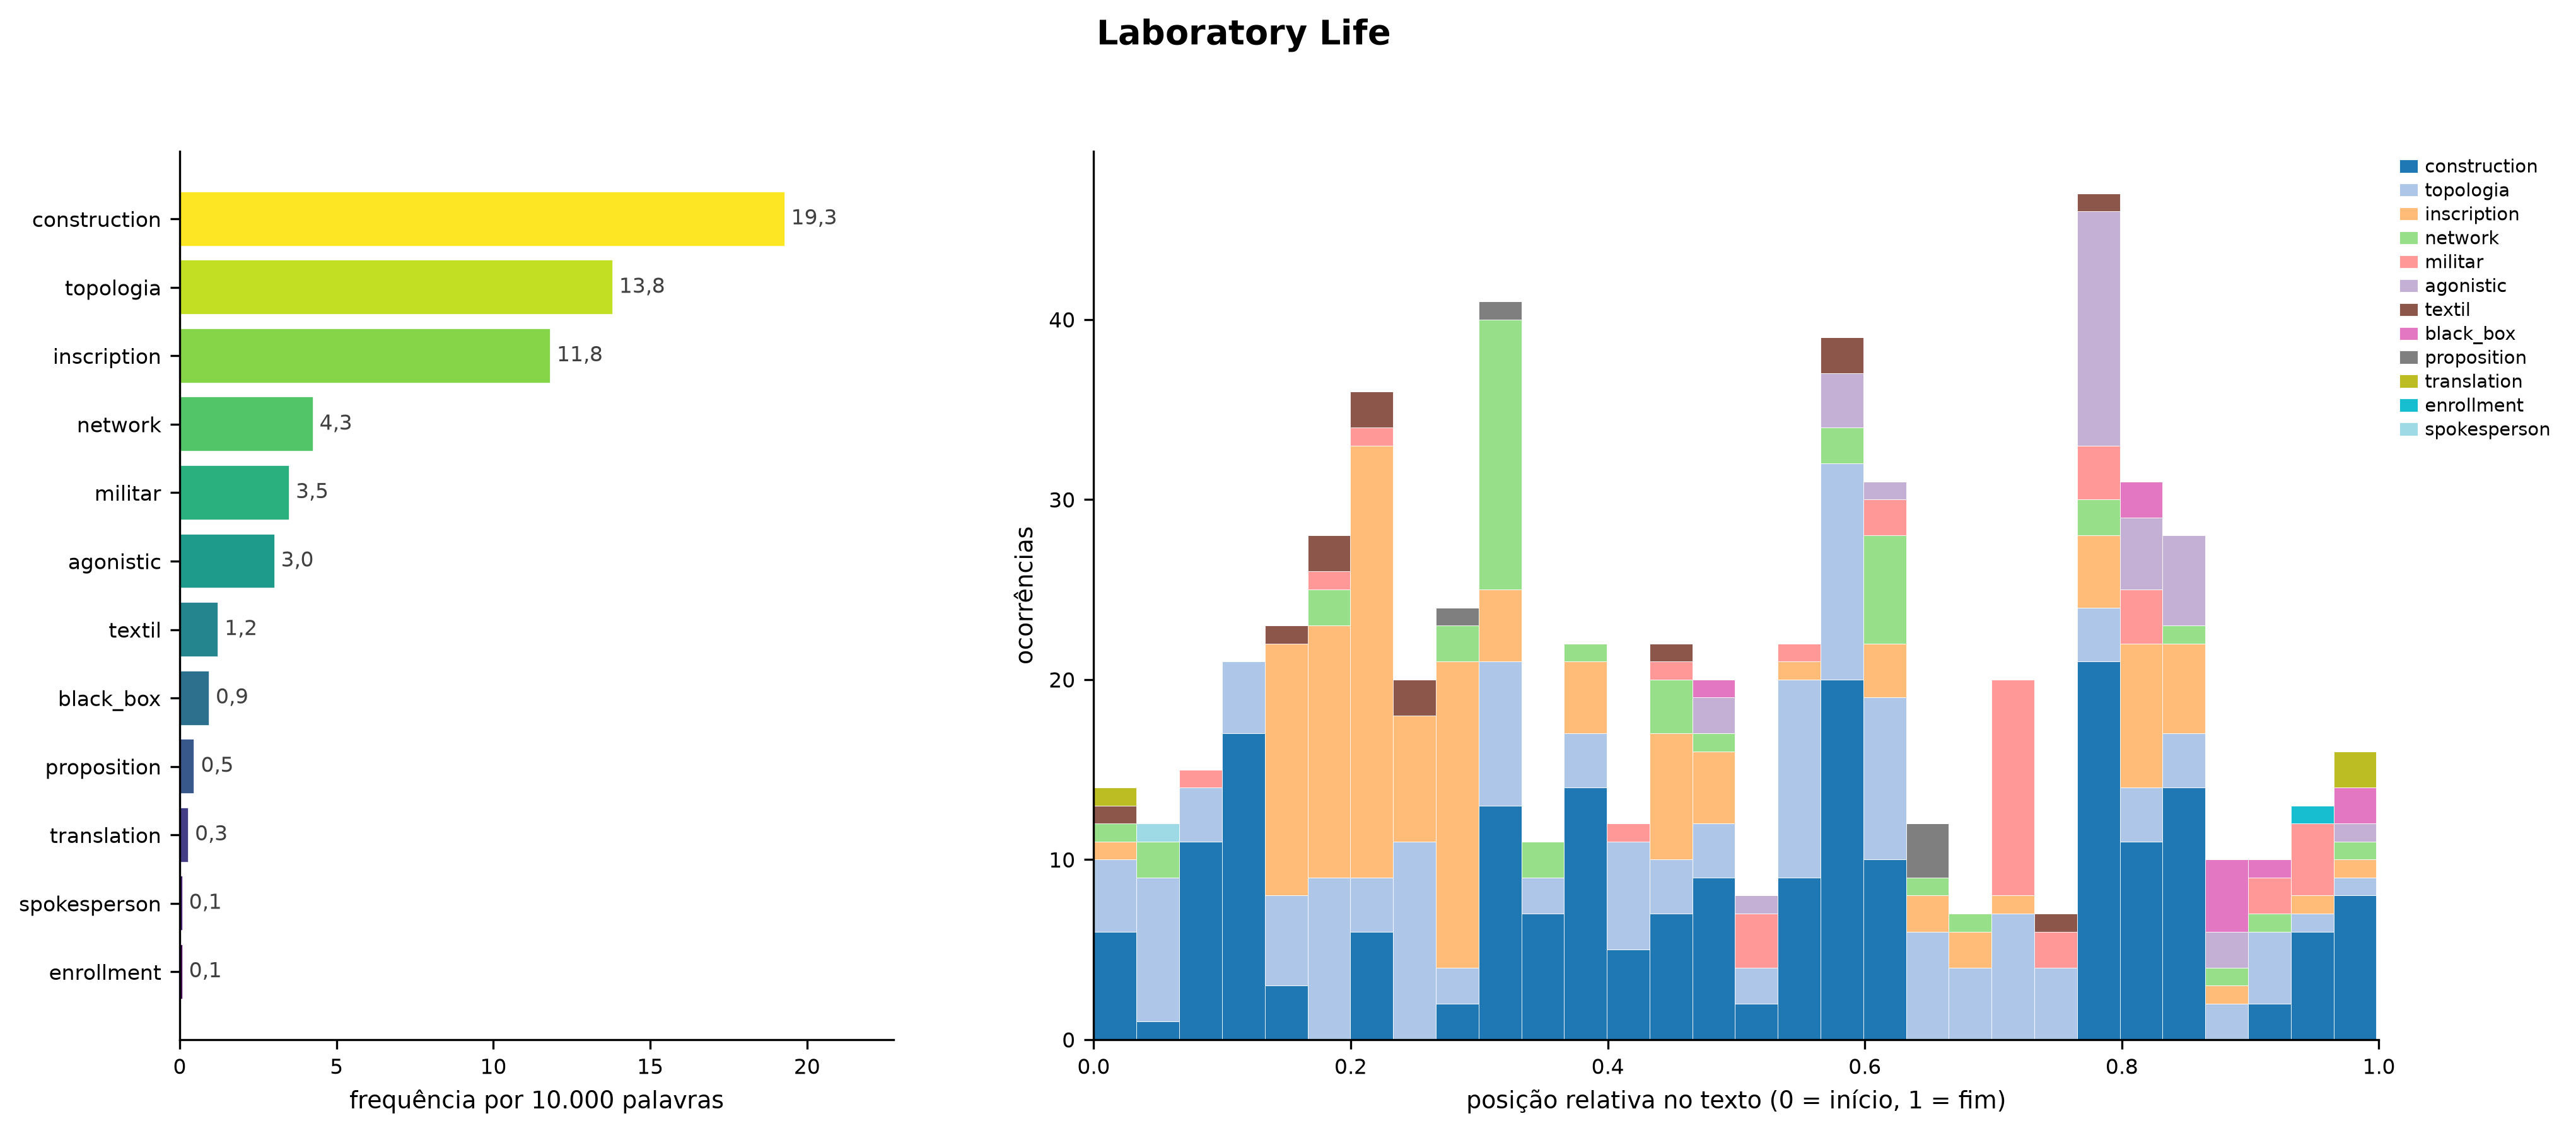
\includegraphics[width=1.0\linewidth]{figuras/cap.2/lexicometria/etapa1_lab_life_freq_e_densidade.png}
\caption[Frequência e distribuição dos rótulos em \emph{Laboratory Life}]{Rótulos do catálogo lexical em \emph{Laboratory Life} (Latour e Woolgar, 1986). À esquerda, a frequência de cada rótulo em ocorrências por dez mil palavras, com o rótulo \texttt{militar} na contagem refinada pela desambiguação de \textit{war}/\textit{wars}; à direita, a distribuição das ocorrências de cada rótulo ao longo do texto, da abertura ao fecho da obra. O vocabulário do construtivismo social, \textit{construction} e \textit{inscription}, domina a frequência, e o rótulo \texttt{militar} aparece em registro contido, coerente com o uso instrumental da analogia militar nesta obra. Fonte: análise das figurações em \url{github.com/julianehelanski/analise-figuracoes-latour}.}
\label{fig:freq_densidade_lab_life}
\end{figure}

% [FIGURA 2] — Science in Action: frequência + densidade.
% Arquivo a regenerar: freq_densidade_sia.png (militar refinado, n=363).
\begin{figure}[htbp]
\centering
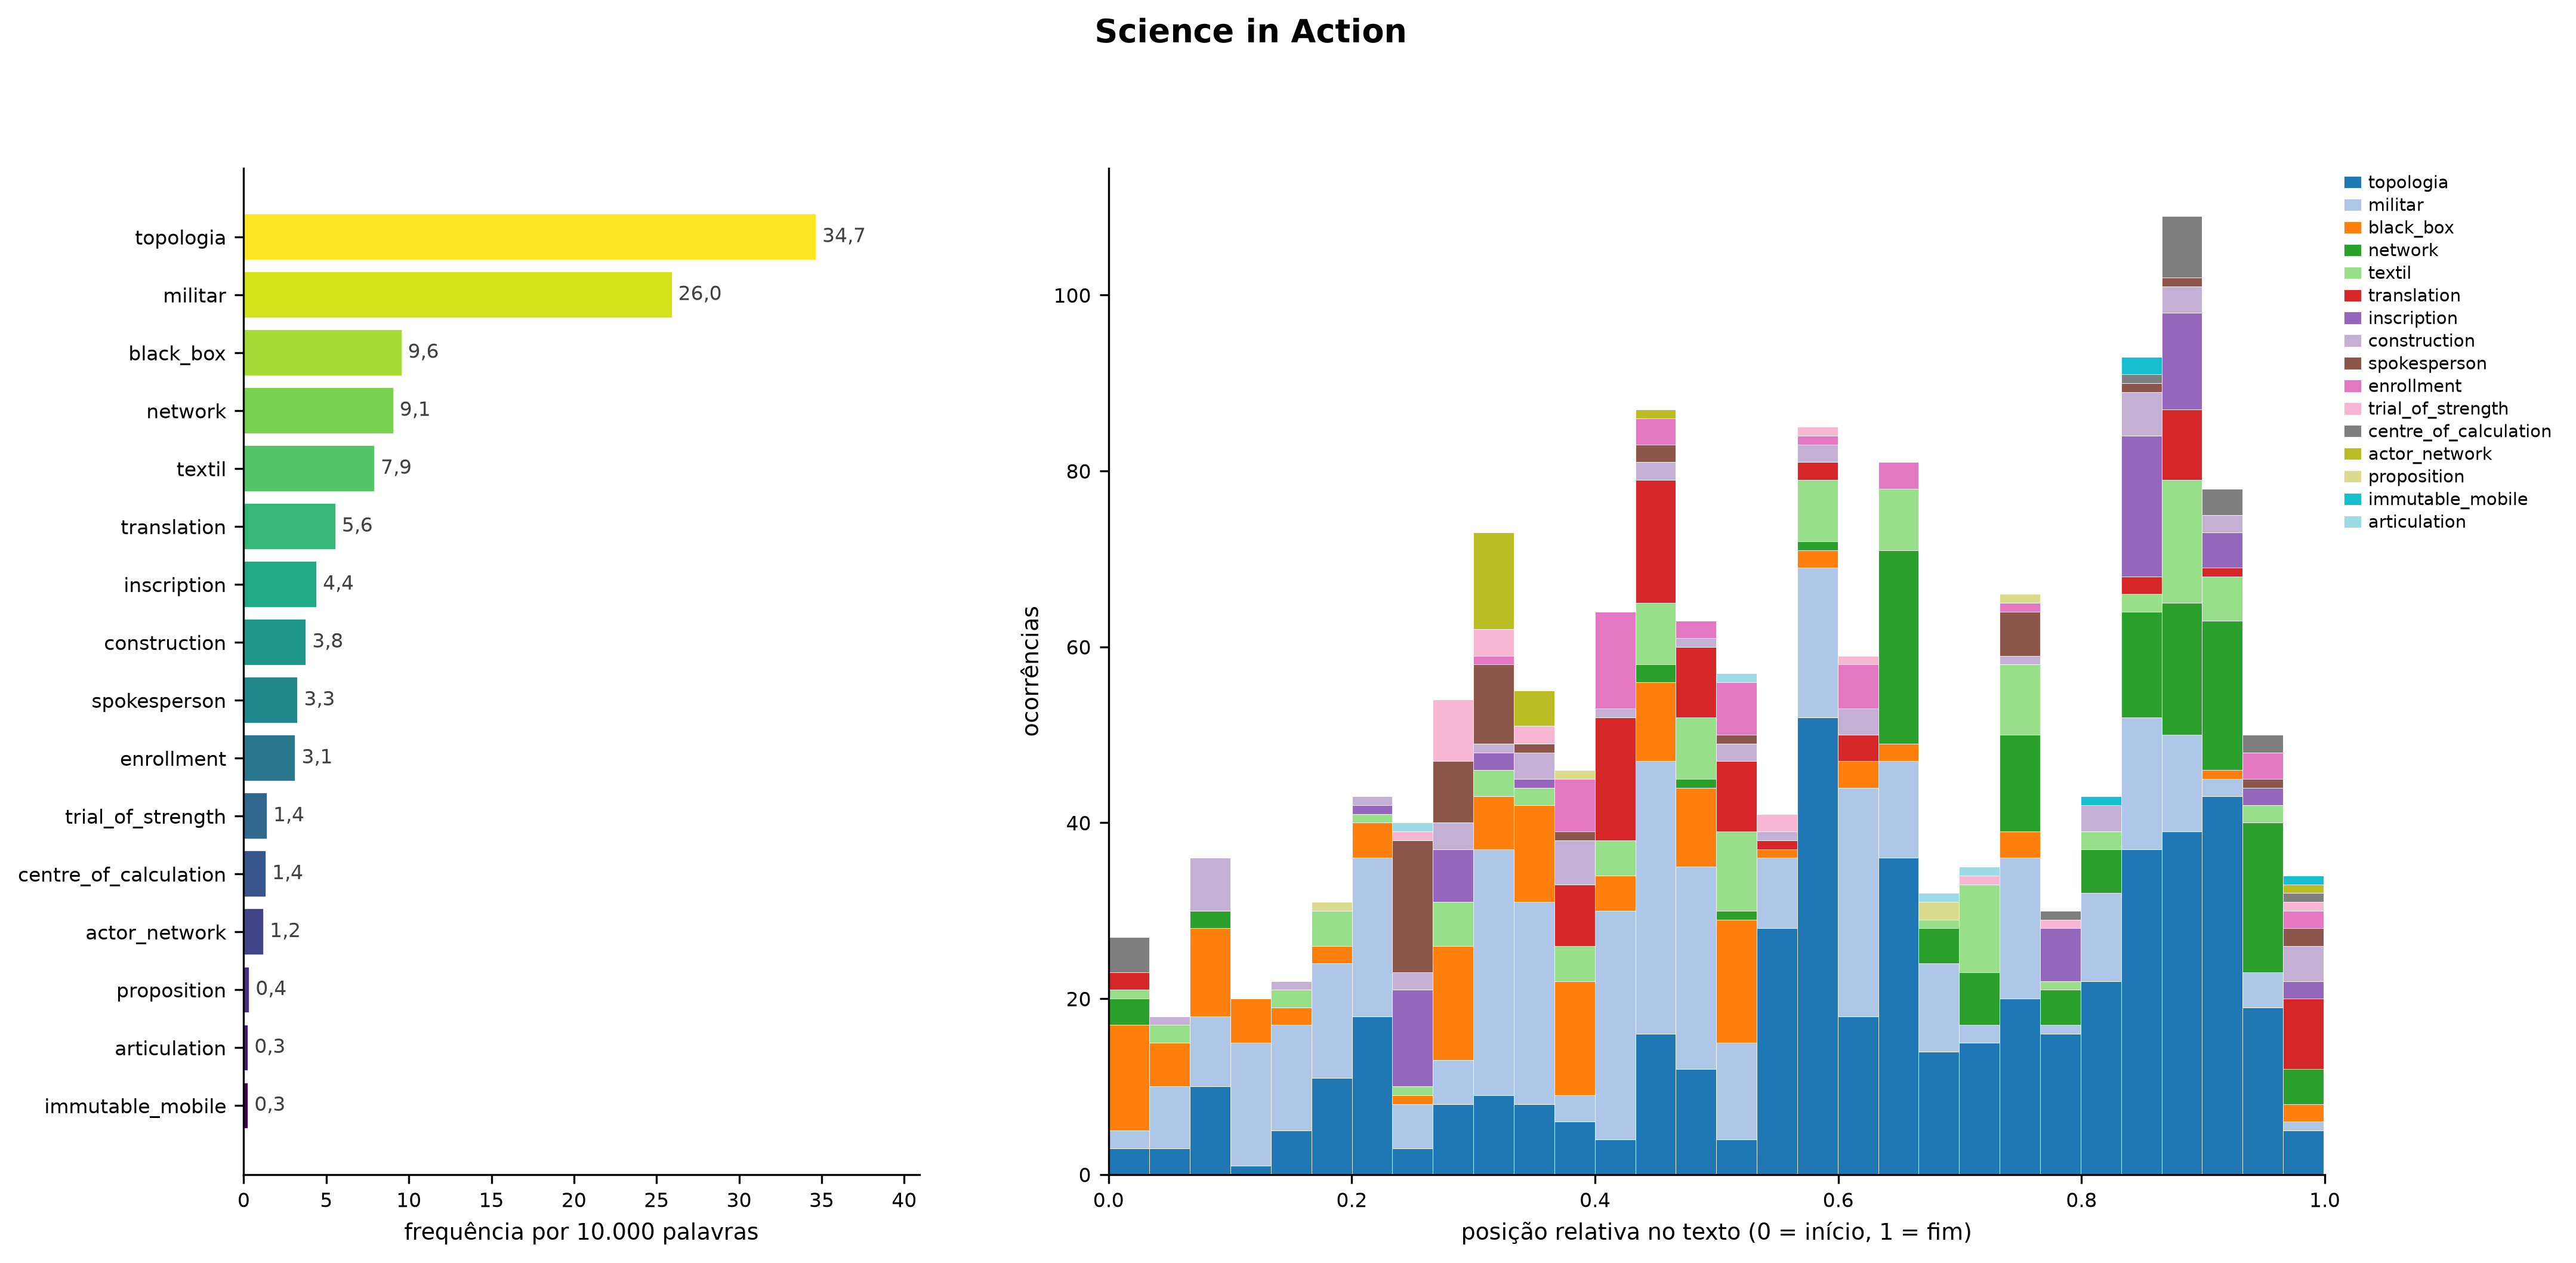
\includegraphics[width=1.0\linewidth]{figuras/cap.2/lexicometria/etapa1_sia_freq_e_densidade.png}
\caption[Frequência e distribuição dos rótulos em \emph{Science in Action}]{Rótulos do catálogo lexical em \emph{Science in Action} (Latour, 1987). À esquerda, a frequência de cada rótulo em ocorrências por dez mil palavras, com o rótulo \texttt{militar} na contagem refinada; à direita, a distribuição das ocorrências ao longo do texto. O rótulo \texttt{militar} encabeça a frequência ao lado de \texttt{topologia}, e a distribuição mostra o vocabulário militar espalhado por toda a extensão da obra. Fonte: análise das figurações em \url{github.com/julianehelanski/analise-figuracoes-latour}.}
\label{fig:freq_densidade_sia}
\end{figure}

% [FIGURA 3] — Pandora's Hope: frequência + densidade.
% Arquivo a regenerar: freq_densidade_pandora.png (militar refinado, n=156).
\begin{figure}[htbp]
\centering
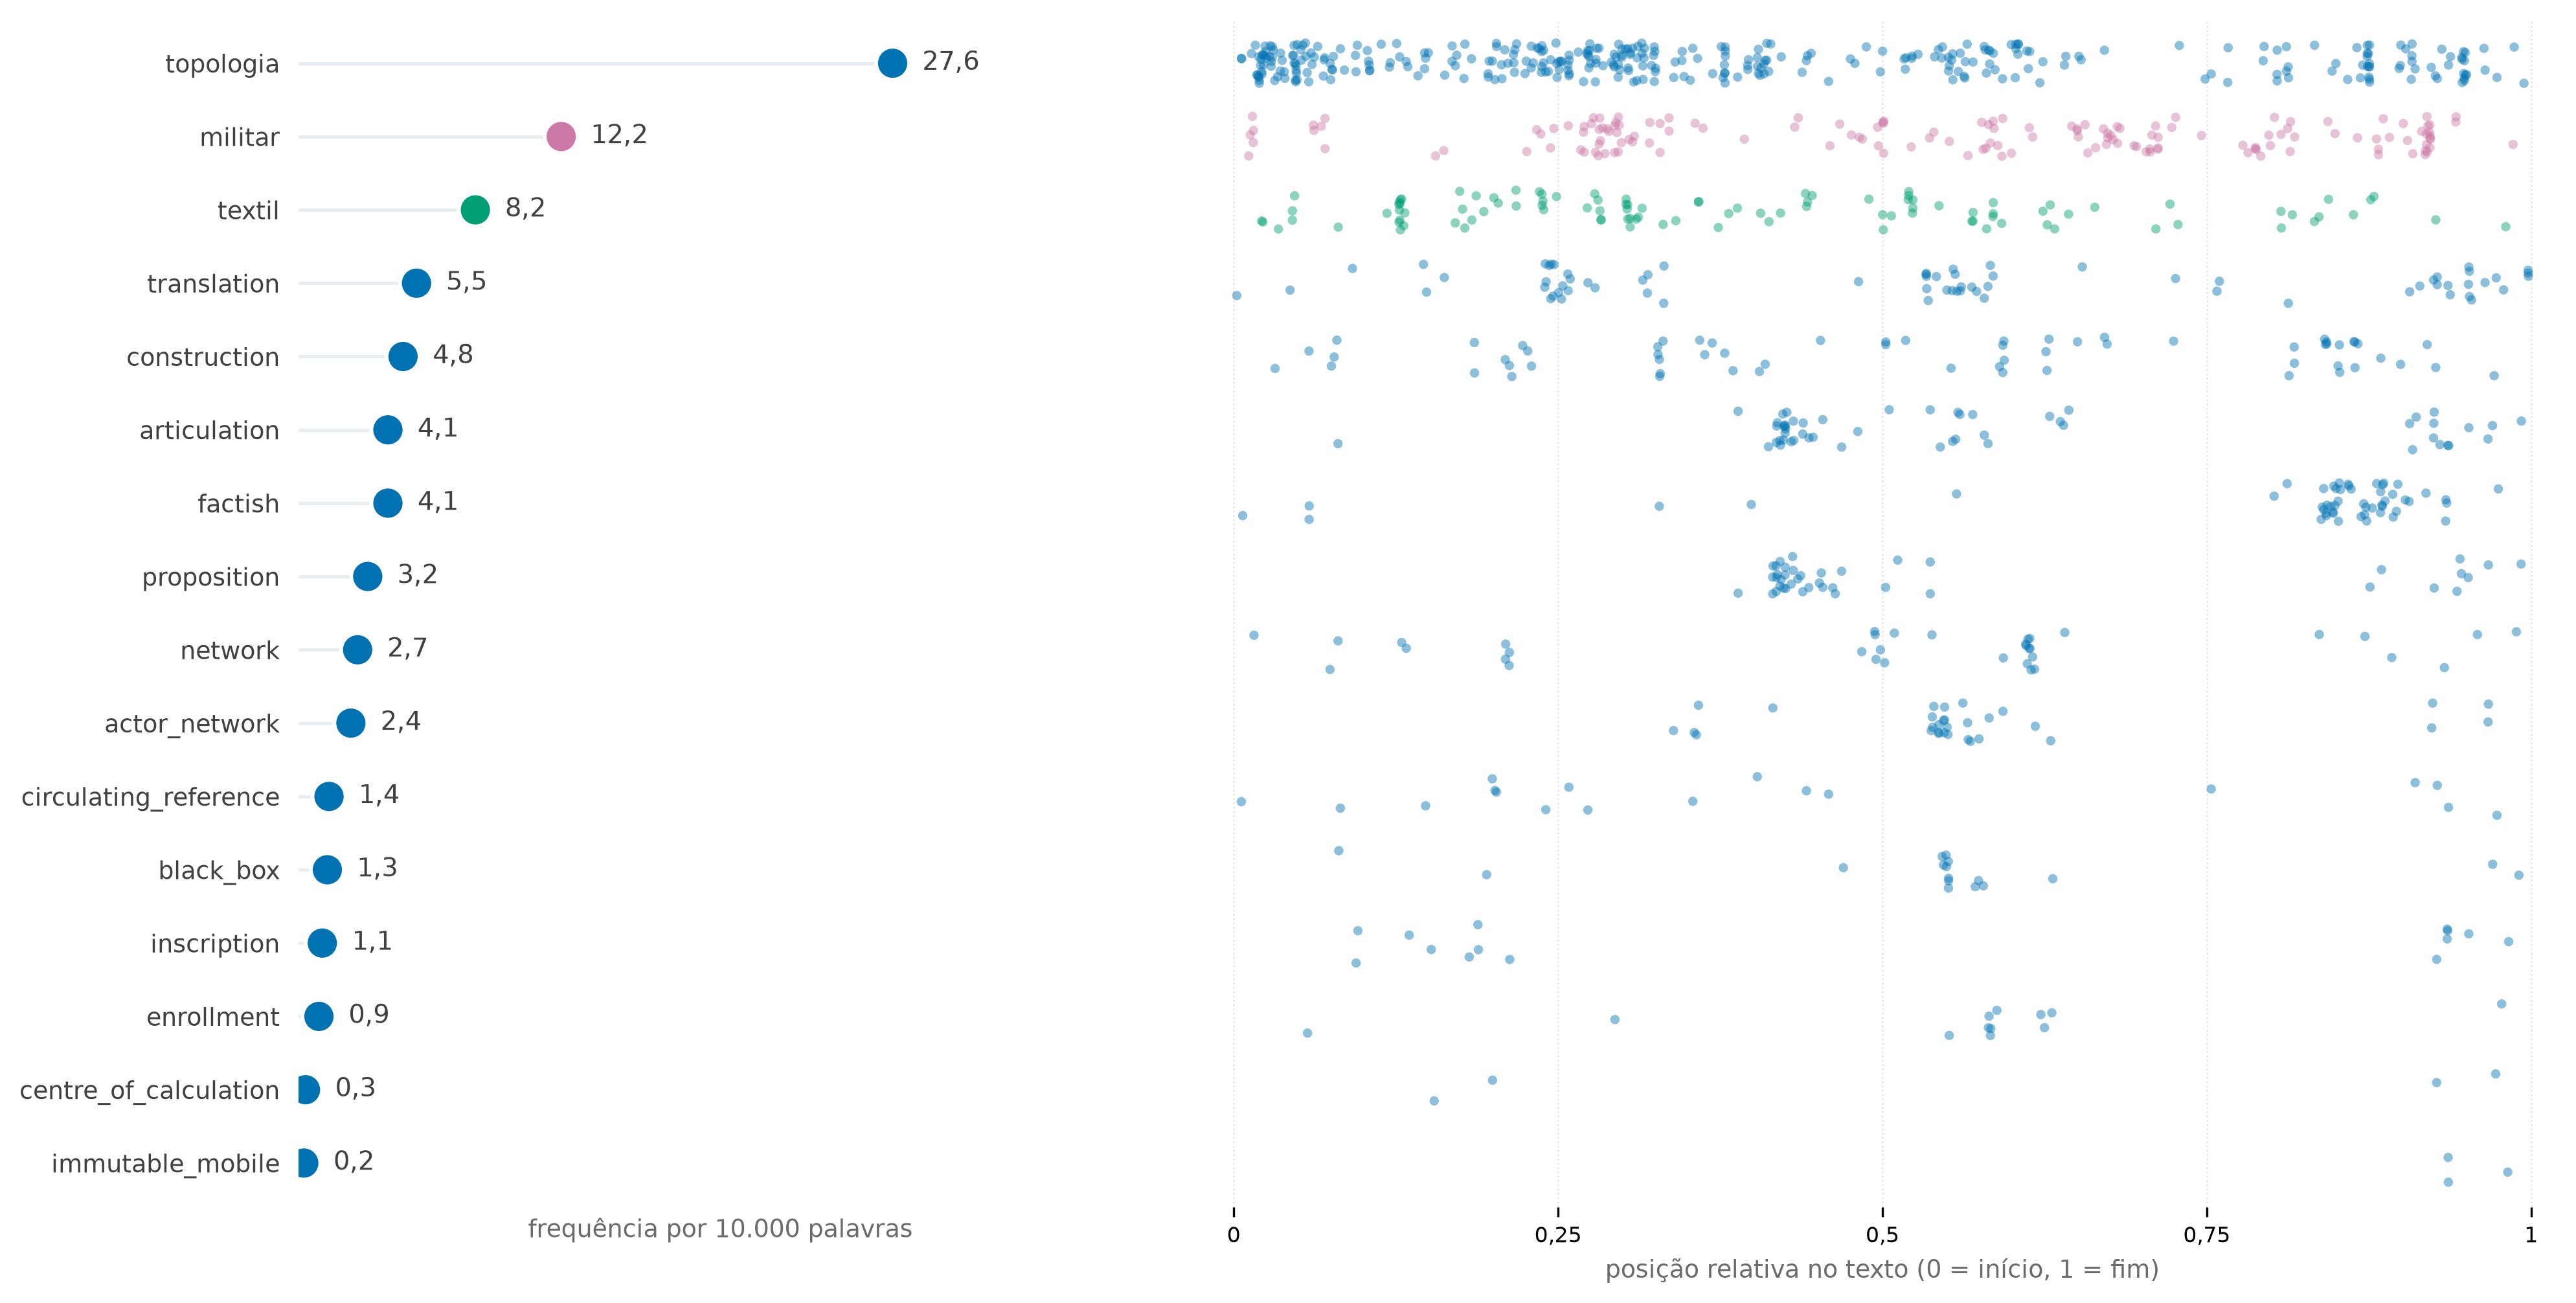
\includegraphics[width=1.0\linewidth]{figuras/cap.2/lexicometria/etapa1_pandora_freq_e_densidade.png}
\caption[Frequência e distribuição dos rótulos em \emph{Pandora's Hope}]{Rótulos do catálogo lexical em \emph{Pandora's Hope} (Latour, 1999). À esquerda, a frequência de cada rótulo em ocorrências por dez mil palavras, com o rótulo \texttt{militar} na contagem refinada; à direita, a distribuição das ocorrências ao longo do texto. O rótulo \texttt{militar} mantém-se em registro alto treze anos depois de \emph{Science in Action}, e a distribuição mostra o vocabulário militar concentrado em picos isolados, em especial na faixa do capítulo sobre Frédéric Joliot e na do epílogo, em contraste com a distribuição contínua de 1987. Fonte: análise das figurações em \url{github.com/julianehelanski/analise-figuracoes-latour}.}
\label{fig:freq_densidade_pandora}
\end{figure}

% [NOTA DE REVISÃO 8] Parágrafo de leitura das figuras por obra.
% Antes este parágrafo lia uma única figura comparativa e remetia a
% uma tabela e a uma segunda figura, ambas removidas. Reescrito para
% ler as três figuras compostas por obra. Os números essenciais
% (3,50 / 25,95 / 12,19 e a substituição agonistic->trial_of_strength)
% sobrevivem no corpo. Regra 4: sem "não X mas Y".
As Figuras~\ref{fig:freq_densidade_lab_life}, \ref{fig:freq_densidade_sia} e~\ref{fig:freq_densidade_pandora} apresentam, obra a obra, a frequência de cada rótulo ao lado da distribuição das ocorrências ao longo do texto. A leitura conjunta das três sustenta dois achados. O primeiro é a magnitude do salto entre \emph{Laboratory Life} e \emph{Science in Action}. Em \emph{Laboratory Life}, escrito com Woolgar, a densidade do rótulo \texttt{militar} fica em 3,50 ocorrências por dez mil palavras, e o vocabulário que domina a obra é o do construtivismo social, \textit{construction} e \textit{inscription};\footnote{O rótulo \texttt{topologia}, que acrescentei ao catálogo na etapa~2 e que apresento adiante, registra em \emph{Laboratory Life} densidade de 13,81 ocorrências por dez mil palavras, valor que o situa entre os rótulos de maior densidade da obra, acima de \textit{inscription}. As Figuras~\ref{fig:freq_densidade_lab_life} a~\ref{fig:freq_densidade_pandora} foram mantidas com os dezessete rótulos da etapa~1 e por isso não exibem o rótulo \texttt{topologia}; a sua densidade nas três obras monográficas consta da contagem do catálogo estendido que apresento na seção seguinte.} em \emph{Science in Action}, escrito por Latour um ano depois, a densidade do rótulo \texttt{militar} salta para 25,95 por dez mil, um aumento de mais de sete vezes, e a figuração militar passa a encabeçar a frequência da obra. O segundo achado é a manutenção da densidade militar em registro alto em \emph{Pandora's Hope}, treze anos depois: 12,19 por dez mil palavras na contagem refinada, ainda mais de três vezes a densidade de \emph{Laboratory Life}. A figuração militar-industrial que se cristaliza em \emph{Science in Action} permanece em registro alto quando Latour, em \emph{Pandora's Hope}, tenta reformular o estatuto ontológico dos fatos científicos pelas noções de \textit{factish} e \textit{circulating reference}. A coluna de distribuição das três figuras acrescenta uma leitura que a frequência sozinha não devolve: no primeiro dos dois livros solo o vocabulário militar se espalha por toda a extensão do texto, ao passo que no segundo ele se concentra em picos isolados, em especial na faixa do capítulo sobre Frédéric Joliot e a fabricação do reator de Ivry às vésperas da Segunda Guerra Mundial e na do epílogo. O contraste entre as duas distribuições sustenta a leitura de que, em \emph{Science in Action}, a figuração militar funciona como prosa argumentativa, e que, em \emph{Pandora's Hope}, ele se concentra em momentos específicos no argumento. O KWIC, \textit{keyword in context}, confirma o registro descritivo de \emph{Science in Action}: os termos que dominam a contagem aparecem sem aspas distanciadoras, como em \enquote{technoscience is part of a war machine and should be studied as such} \parencite[p.~192]{Latour1987Science}.\footnote{Tradução brasileira: \textcite{Latour2011CienciaEmAcao}, p.~\texttt{[p. 269]}.} As três figuras compostas têm escalas de frequência independentes, próprias a cada obra, e por isso a comparação direta de magnitude entre elas pede uma quarta figura. A Figura~\ref{fig:comparacao_tres_obras} põe as três obras na mesma escala de densidade e torna o salto imediatamente legível: o rótulo \texttt{militar} passa de 3,50 ocorrências por dez mil palavras em 1986 a 25,95 em 1987, e se mantém em 12,19 em 1999.

A densidade dos rótulos surgem do encontro entre três coisas: das obras que Latour escreveu, do catálogo de rótulos que eu construí e da janela de contexto que defini para contar as ocorrências. Um catálogo com mais rótulos e mais termos por rótulo registra mais ocorrências e mais co-ocorrências (proximidade textual), e uma janela mais ampla aproxima mais termos; a densidade que vejo na figura responde a essas escolhas tanto quanto responde à escrita de Latour. Isso não retira valor à medida, e tampouco a relativiza ao ponto de torná-la arbitrária: significa que a densidade só sustenta o argumento quando eu a leio de modo situado, na comparação entre obras analisadas sob o mesmo catálogo e a mesma janela, e quando declaro o instrumento com que a produzi. É por essa razão que mantenho o catálogo e a janela constantes nas cinco obras das etapas~1 e~2, e que apresento as figuras obra a obra antes de qualquer comparação agregada, isso significa que a comparabilidade é uma das condição que eu construo. Tomada assim, a variação de densidade entre as obras deixa de ser um número a constatar e passa a delinear a variedade de registros figurativos com que Latour descreveu a tecnociência e a teoria ao longo dessa seis obras e aqui as interpreto como uma trajetória intelectual. 

A cristalização do léxico militar em \emph{Science in Action} acompanha-se da substituição interna ao catálogo que descrevi acima. O termo \textit{agonistic}, que em \emph{Laboratory Life} aparece trinta e duas vezes e descreve o campo em que enunciados são testados, desaparece completamente em \emph{Science in Action} e em \emph{Pandora's Hope}. Em outra direção, \textit{trial of strength} surge pela primeira vez em \emph{Science in Action}, com vinte ocorrências, e descreve um gesto semelhante ao do agon: \enquote{trials of strength to evaluate the resistance of the ties that link the representatives to what they speak for} \parencite[p.~93]{Latour1987Science}.\footnote{Tradução brasileira: \textcite{Latour2011CienciaEmAcao}, p.~\texttt{[p. 118]}.} A substituição, do agon ao julgamento de força, marca um deslocamento do registro pragmático-filosófico, em que o agon nomeia o jogo da prova com um vocabulário herdado da retórica clássica, para um registro topológico-militar, em que a prova é medida por resistências, laços e mobilizações. O agon perde o estatuto de figura organizadora, e o vocabulário militar passa a ocupar o seu lugar com uma densidade que, como mostra a figura~\ref{fig:freq_densidade_sia}, é a marca distintiva de \emph{Science in Action} no conjunto do corpus.\footnote{A desambiguação de \textit{war}/\textit{wars} descrita acima incide de modo desigual sobre as três obras, e é esse efeito desigual que sustenta o seu uso: a queda do rótulo \texttt{militar} é de 26,4\% em \emph{Pandora's Hope}, ao passo que em \emph{Science in Action} é de 2,9\% e em \emph{Laboratory Life} de 5,1\%. O pico de \emph{Science in Action} permanece, assim, como ponto de cristalização da figuração militar-industrial em registro figurativo mesmo depois de descontado o uso histórico de \textit{war}.}

A morfologia da distribuição do léxico militar ao longo dos textos, visível nos painéis de densidade das figuras~\ref{fig:freq_densidade_sia} e~\ref{fig:freq_densidade_pandora}, sustenta uma leitura adicional sobre o estatuto que o rótulo \texttt{militar} ocupa em cada obra. Em \emph{Science in Action}, a distribuição é contínua e relativamente homogênea, com vários picos médios distribuídos por praticamente toda a extensão do texto: o vocabulário militar não está confinado a uma seção ou capítulo, atravessa transversalmente a obra e funciona de forma recorrente à prosa argumentativa. Em \emph{Pandora's Hope}, a distribuição apresenta picos mais altos e isolados, separados por trechos longos de densidade baixa ou nula, e os picos correspondem em sua maioria ao capítulo sobre a trajetória de Frédéric Joliot e a fabricação do reator de Ivry e ao epílogo da obra. Essa distribuição sustenta a leitura de que, em \emph{Pandora's Hope}, o vocabulário militar se concentra em momentos argumentativamente situados, enquanto em \emph{Science in Action} ele se distribui em camadas descritivas contínuas das práticas tecnocientíficas.

A contagem de co-ocorrências completa essa leitura. Calculei a co-ocorrência entre os rótulos do catálogo em janelas de duzentas palavras, sobre o texto integral de \emph{Science in Action}, e o resultado é uma matriz que cruza cada rótulo com todos os demais.\footnote{A matriz de co-ocorrência conta o rótulo \texttt{militar} na contagem bruta, e não na refinada pela desambiguação de \textit{war}/\textit{wars} que adoto no restante deste capítulo~\ref{capitulo2}. O cálculo da co-ocorrência incide sobre o arquivo de \textit{keyword in context} antes do refinamento, e refinar a matriz exigiria reprocessar a co-ocorrência sobre um KWIC já refinado. Registro a opção como limitação conhecida, documentada no repositório, e observo que ela não desloca a ordem de grandeza nem a hierarquia dos pares que reporto.} A leitura dessa matriz mostra um ponto que a contagem agregada, rótulo a rótulo, não devolve. O par mais denso de toda a rede de co-ocorrência de \emph{Science in Action} é \texttt{militar}--\texttt{topologia}, com quatrocentas e noventa e cinco co-ocorrências, valor que supera em mais de três vezes o do par \texttt{militar}--\textit{black box}. O vocabulário militar e o vocabulário topológico, que esta tese reconhece, ao lado do têxtil, como o polo que tensiona a figuração militar-industrial, já aparecem entrelaçados em \emph{Science in Action}, na obra de 1987, antes dos artigos metateóricos em que Latour passa a refletir sobre a sua própria teoria. A densidade desse entrelaçamento não é um caso isolado na matriz, os três pares mais densos depois de \texttt{militar}--\texttt{topologia} são \texttt{network}--\texttt{topologia}, com trezentas e sessenta co-ocorrências, \texttt{textil}--\texttt{topologia}, com cento e sessenta e seis, e \texttt{militar}--\texttt{textil}, com cento e cinquenta e cinco, e os quatro pares reúnem o vocabulário militar, o topológico e o têxtil já na obra que cristaliza a figuração militar-industrial. O vocabulário militar aparece, ainda, em vizinhança dos conceitos pelos quais a teoria ator-rede foi recebida como descrição da prática científica: na mesma janela de duzentas palavras, o rótulo \texttt{militar} co-ocorre cento e cinquenta e duas vezes com \textit{black box}, noventa e oito com \textit{network}, setenta e duas com \textit{inscription} e setenta e uma com \textit{translation}, além de cinquenta e nove vezes com \textit{construction}, cinquenta e cinco com \textit{spokesperson} e cinquenta e duas com \textit{enrollment}. Os termos pelos quais a teoria circulou como descrição neutra, \textit{black box}, \textit{network}, \textit{translation} e \textit{inscription}, aparecem, no texto de 1987, na vizinhança recorrente tanto do vocabulário militar quanto do vocabulário topológico. A matriz de co-ocorrência completa, rótulo a rótulo, fica versionada no repositório.

\begin{figure}[htbp]
\centering
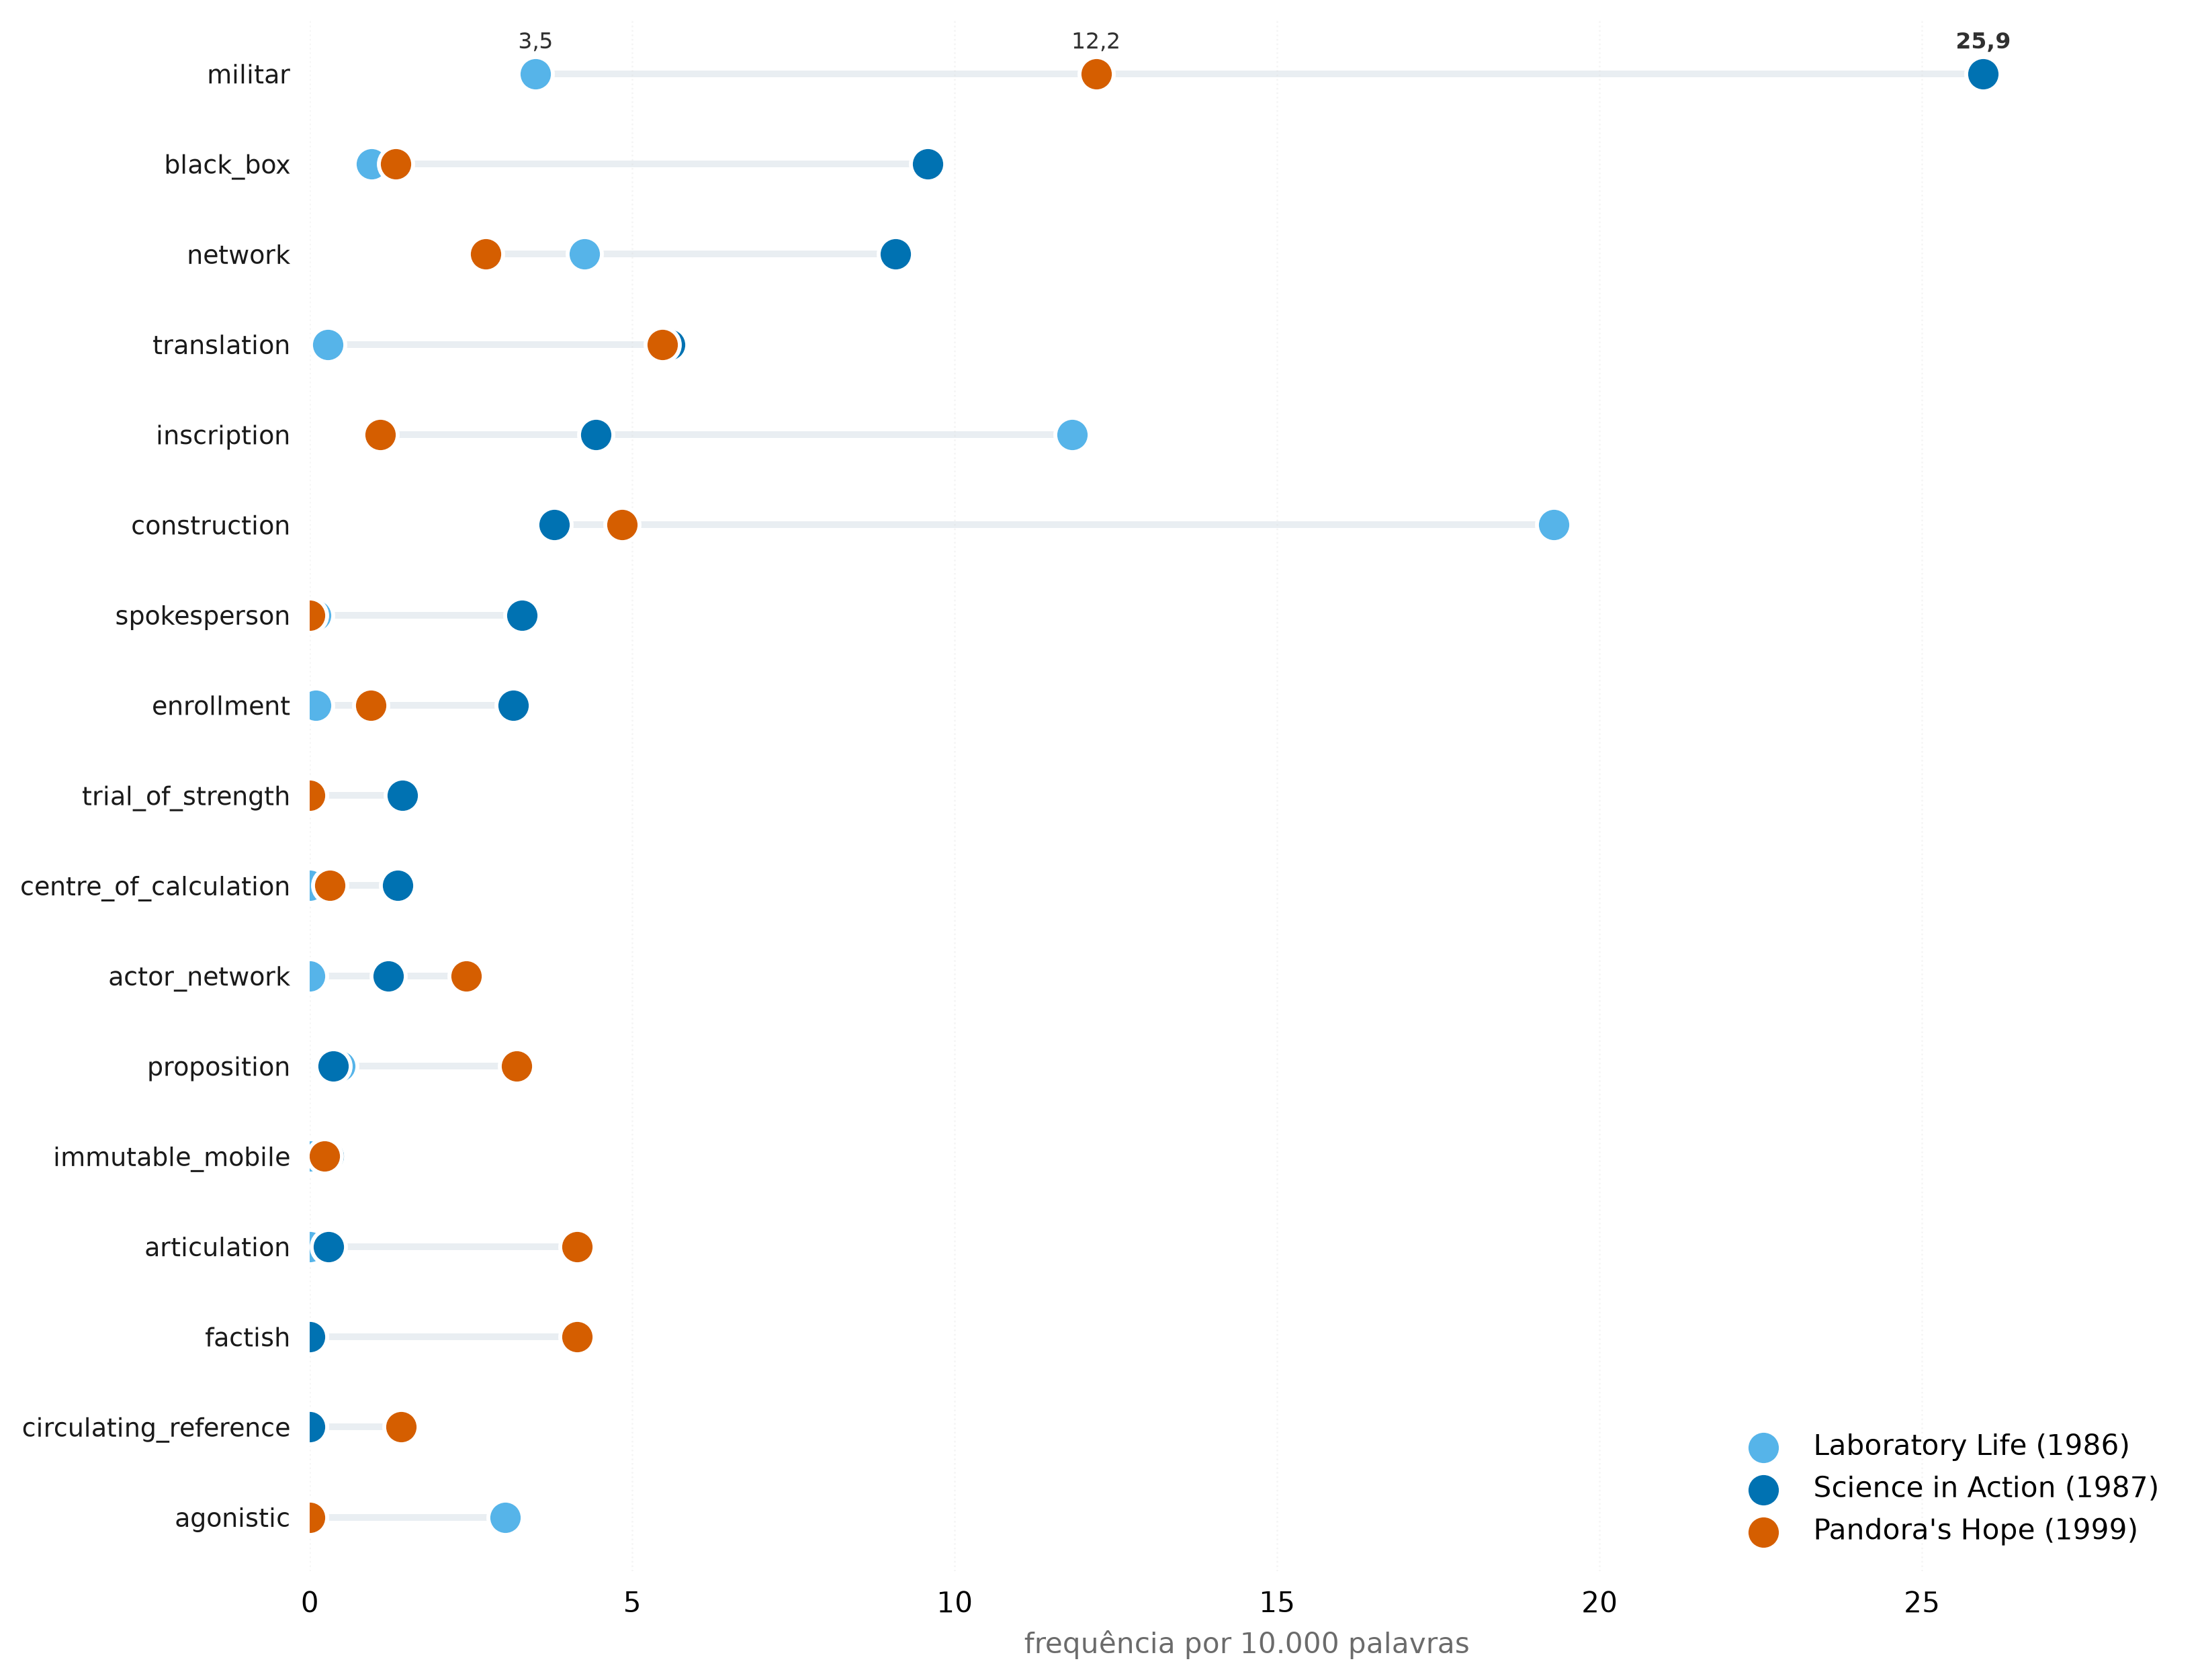
\includegraphics[width=0.85\linewidth]{figuras/cap.2/lexicometria/etapa1_passo4_comparacao_frequencias_tres_obras.png}
\caption[Densidade comparada dos rótulos nas três obras de Latour]{Densidade dos dezessete rótulos do catálogo lexical nas três obras de Latour em escopo da etapa~1, \emph{Laboratory Life} (1986), \emph{Science in Action} (1987) e \emph{Pandora's Hope} (1999), em ocorrências por dez mil palavras e em escala comum às três obras. Cada rótulo é uma linha, e os três pontos ligados pela linha-guia correspondem às três obras em ordem cronológica de publicação, \emph{Laboratory Life} em azul claro, \emph{Science in Action} em azul e \emph{Pandora's Hope} em vermelho. O rótulo \texttt{militar} aparece no topo, com a maior amplitude entre as três obras, na contagem refinada pela desambiguação simétrica de \textit{war}/\textit{wars}, com os valores 3,50 em 1986, 25,95 em 1987 e 12,19 em 1999 anotados acima dos seus pontos. A escala comum às três obras torna legível o salto na densidade do rótulo \texttt{militar} entre 1986 e 1987 e a sua manutenção em registro alto em 1999. Fonte: análise das figurações em \url{github.com/julianehelanski/analise-figuracoes-latour}.}
\label{fig:comparacao_tres_obras}
\end{figure}

A etapa~1 alcançou os dezessete rótulos do catálogo, e o relatório completo, com a matriz cruzada e os rankings por obra individual, fica disponível no repositório.\footnote{O relatório consolidado e a matriz cruzada completa dos dezessete rótulos por obra estão em \url{github.com/julianehelanski/analise-figuracoes-latour}, na pasta de \emph{outputs}. Os rankings de frequência interna, os mapas de densidade ao longo do texto e as redes de co-ocorrência calculados obra a obra ficam nas subpastas de cada obra.} O que retenho aqui da etapa~1 é o que dá nome ao ponto sensível da escrita latouriana: a figuração militar-industrial que descrevi por leitura de passagens escolhidas aparece como resultado contável da escrita que Latour produziu em \emph{Science in Action} e manteve, em densidade atenuada e ainda dominante, em \emph{Pandora's Hope}. A análise corroborou a leitura qualitativa que eu sustentava por amostras, e ofereceu medida sistemática da magnitude do deslocamento de \emph{Laboratory Life} a \emph{Pandora's Hope}, em forma auditável.

% =====================================================================
% ETAPA 2 e ETAPA 2-bis
% =====================================================================
\subsection{O corpus estendido: o vocabulário metateórico de \emph{Clarifications} e \emph{On Recalling ANT}}
\label{subsubsec:trajetoria_estendida_metateorica}

A análise sobre as três obras da etapa 1 faz parte de um trabalho maior, que estendi com a inclusão de dois artigos nos quais Latour propõe uma nova interpretação sobre a teoria ator-rede. A inclusão desses dois artigos vieram de uma leitura anterior em que observei um contraste de posicionamento e conceitual de Latour diferente dos livros. Se o vocabulário militar-industrial é um dos pontos sensíveis da obra de Latour, e o é sobretudo quando passa a explicar a prática tecnocientífica, então é razoável esperar que esse vocabulário se reorganize quando Latour, de modo autorreflexivo, reinterpreta a própria teoria que vinha desenvolvendo. Os dois artigos metateóricos que escolhi para essa etapa da análise, \emph{On Actor-Network Theory: A Few Clarifications}, de 1996 \parencite{latour1996clarifications}, e \emph{On Recalling ANT}, de 1999 \parencite{Latour1999RecallingANT}, são textos curtos em comparação com os três livros, e Latour os escreveu para esclarecer, defender e reformular a teoria ator-rede diante de seus críticos.\footnote{A análise de \emph{On Recalling ANT} incide sobre o texto integral do artigo.} Os dois artigos não descrevem laboratórios, controvérsias ou alianças sociotécnicas, descrevem a teoria que descreve essas coisas. Essa diferença é o ponto de partida da segunda etapa da análise: o que acontece com a densidade dos rótulos quando o objeto da descrição passa de \emph{tecnociência em ação} para \emph{teoria da tecnociência em ação}?

A leitura qualitativa dos dois artigos, anterior à análise lexicométrica, mostrou que eles empregam um vocabulário têxtil-topológico em densidade que os três livros não haviam apresentado, e que o catálogo original não dispunha de rótulo lexical capaz de captar esse vocabulário. Por isso, e em consequência do gesto reflexivo que organiza este capítulo~\ref{capitulo2}, ampliei o catálogo de dezessete para dezenove rótulos, com o acréscimo dos rótulos \texttt{textil} e \texttt{topologia}, sobretudo a partir de \emph{On Actor-Network Theory: A Few Clarifications}.\footnote{Os termos do rótulo \texttt{textil}, entre eles \textit{fabric}, \textit{thread}, \textit{wire}, \textit{string}, \textit{rope}, \textit{capillary}, \textit{fibrous}, \textit{thread-like}, \textit{wiry}, \textit{stringy} e \textit{ropy}, e os termos do rótulo \texttt{topologia}, entre eles \textit{topology}, \textit{node}, \textit{connection}, \textit{flat}, \textit{folded}, \textit{outside}, \textit{circulating}, \textit{flow} e \textit{scale}, foram catalogados a partir de duas passagens-chave: a definição da teoria ator-rede como mudança de topologia em \emph{Clarifications} e a formulação da topologia como \emph{flat and folded} em \emph{On Recalling ANT}. Apliquei o acréscimo simetricamente sobre as cinco obras, e mantive as figuras da etapa~1 com os dezessete rótulos originais, para preservar a coerência da leitura cronológica nas três primeiras obras.} A análise lexicométrica sobre o corpus estendido sustenta três achados que reorganizam a interpretação dos dados dos três livros iniciais. O primeiro achado é a queda do rótulo \texttt{militar} nos dois textos metateóricos: a densidade bruta do rótulo \texttt{militar} cai de 26,74 por dez mil palavras em \emph{Science in Action} para 3,82 em \emph{Clarifications}, valor próximo do que se observa em \emph{Laboratory Life}, de 3,69.\footnote{Adoto a contagem bruta nesta comparação entre as obras porque a desambiguação de \textit{war}/\textit{wars} foi aplicada aos três livros, e a contagem bruta é a base comum que permite comparar as cinco sem assimetria de procedimento. A diferença entre bruta e refinada não altera a ordem de grandeza da queda aqui descrita. \emph{Laboratory Life} é o único dos três livros escrito em coautoria, com Steve Woolgar, e a coincidência entre sua densidade militar e a dos dois artigos metateóricos sugere que a inflexão militar-industrial se consolida com Latour autor solo em \textit{Science in Action}. Todavia, esse dado é insuficiente para sustentar qualquer generalização sobre o efeito da coautoria.} No corpus integral do \emph{Recalling}, a densidade bruta do rótulo \texttt{militar} é de 4,15 por dez mil palavras, correspondente a duas ocorrências, uma descritivo-histórica, \emph{Science Wars}, e uma metalinguística, \emph{alliance} na lista canônica do vocabulário da teoria ator-rede. O segundo achado é a magnitude dos rótulos \texttt{topologia} e \texttt{textil} nos dois artigos: a densidade de \texttt{topologia} salta de 34,68 por dez mil palavras em \emph{Science in Action} para 150,36 em \emph{Clarifications} e 99,48 no \emph{Recalling} integral, três a quatro vezes a densidade observada nos três livros; a densidade de \texttt{textil} salta de 7,94 em \emph{Science in Action} e 8,20 em \emph{Pandora's Hope} para 49,69 em \emph{Clarifications}, mais de seis vezes a densidade média nos três livros. O terceiro achado é a dominância do rótulo \texttt{network} nos dois artigos: 118,50 por dez mil palavras em \emph{Clarifications} e 58,03 no \emph{Recalling} integral, contra 9,08 em \emph{Science in Action} e 2,73 em \emph{Pandora's Hope}.

\begin{longtable}{@{}p{0.23\textwidth} p{0.20\textwidth} p{0.49\textwidth}@{}}
\caption[Catálogo lexical das etapas 1 e 2]{Catálogo lexical das etapas 1 e 2: os dezenove rótulos rastreados nas obras de Latour, com a procedência de cada rótulo e uma amostra dos termos que o definem. A amostra segue a ordem do arquivo de definição: rótulos com até oito termos aparecem completos, rótulos maiores trazem os oito primeiros termos seguidos de \enquote{entre outros}. A lista completa de termos está no repositório, em \url{github.com/julianehelanski/analise_figuracoes/tree/main/campos_lexicais}.}\label{tab:catalogo-etapas12}\\
\toprule
Campo & Procedência & Amostra de termos do catálogo \\
\midrule
\endfirsthead
\caption[]{Catálogo lexical das etapa s 1 e 2 (continuação).}\\
\toprule
Campo & Procedência & Amostra de termos do catálogo \\
\midrule
\endhead
\midrule
\multicolumn{3}{r@{}}{\footnotesize continua na próxima página}\\
\endfoot
\bottomrule
\endlastfoot
\texttt{inscription} & conceito de Latour & \texttt{inscription}, \texttt{inscriptions}, \texttt{inscription device}, \texttt{inscription devices}, \texttt{literary inscription} \\
\texttt{immutable\_mobile} & conceito de Latour & \texttt{immutable mobile}, \texttt{immutable mobiles} \\
\texttt{black\_box} & conceito de Latour & \texttt{black box}, \texttt{black-box}, \texttt{black boxes}, \texttt{blackbox}, \texttt{blackboxing}, \texttt{black-boxing} \\
\texttt{centre\_of\_calculation} & conceito de Latour & \texttt{centre of calculation}, \texttt{center of calculation}, \texttt{centres of calculation}, \texttt{centers of calculation} \\
\texttt{actor\_network} & conceito de Latour & \texttt{actor-network}, \texttt{actor network}, \texttt{actant}, \texttt{actants} \\
\texttt{translation} & conceito de Latour & \texttt{translation}, \texttt{translations}, \texttt{translate}, \texttt{translates}, \texttt{translated} \\
\texttt{trial\_of\_strength} & conceito de Latour & \texttt{trial of strength}, \texttt{trials of strength} \\
\texttt{factish} & conceito de Latour & \texttt{factish}, \texttt{factishes} \\
\texttt{circulating\_reference} & conceito de Latour & \texttt{circulating reference}, \texttt{circulating references} \\
\texttt{articulation} & conceito de Latour & \texttt{articulation}, \texttt{articulations}, \texttt{articulate}, \texttt{articulated} \\
\texttt{construction} & conceito de Latour & \texttt{construction}, \texttt{constructed}, \texttt{constructing}, \texttt{social construction} \\
\texttt{proposition} & conceito de Latour & \texttt{proposition}, \texttt{propositions} \\
\texttt{network} & conceito de Latour & \texttt{network}, \texttt{networks}, \texttt{networking} \\
\texttt{agonistic} & conceito de Latour & \texttt{agonistic}, \texttt{agonistics}, \texttt{agonistic field} \\
\texttt{enrollment} & conceito de Latour & \texttt{enrollment}, \texttt{enrolment}, \texttt{enroll}, \texttt{enrol}, \texttt{enrolled} \\
\texttt{spokesperson} & conceito de Latour & \texttt{spokesperson}, \texttt{spokespersons}, \texttt{spokesman}, \texttt{spokesmen}, \texttt{spokeswoman} \\
\texttt{militar} & rótulo reunido & \texttt{ally}, \texttt{allies}, \texttt{allied}, \texttt{alliance}, \texttt{alliances}, \texttt{enemy}, \texttt{enemies}, \texttt{enmity}, entre outros \\
\texttt{textil} & rótulo reunido & \texttt{thread}, \texttt{threads}, \texttt{threading}, \texttt{threaded}, \texttt{thread-like}, \texttt{threadlike}, \texttt{weave}, \texttt{weaves}, entre outros \\
\texttt{topologia} & rótulo reunido & \texttt{fluid}, \texttt{fluids}, \texttt{fluidity}, \texttt{surface}, \texttt{surfaces}, \texttt{node}, \texttt{nodes}, \texttt{connection}, entre outros \\
\end{longtable}

A partir desses três deslocamentos fiz uma desambiguação simétrica à que apliquei ao rótulo \texttt{militar} nos três livros. A análise refinada do rótulo \texttt{militar} nos dois artigos chega a zero em todas as versões do corpus: as três ocorrências em \emph{Clarifications}, \textit{allies}, \textit{enemies} e \textit{alliance}, e as duas ocorrências no \emph{Recalling} integral foram todas classificadas como uso bibliográfico, metalinguístico, descritivo-histórico ou de polêmica conceitual, e nenhuma aparece como tropo figurativo internamente latouriano. \emph{Clarifications} traz \textit{alliance} apenas na referência bibliográfica a \emph{La nouvelle alliance} de Prigogine e Stengers; \textit{allies} aparece em formulação que polemiza com a leitura corrente da teoria ator-rede como rede de aliados homens em luta por poder, formulação que Latour cita para rejeitar e que descreve como \enquote{about as accurate as saying that the night sky is black because the astrophysicists have shown there is a big black hole in it} \parencite[p.~5]{latour1996clarifications}; \textit{enemies} aparece em contexto epistemológico sobre os \enquote{reflexivists} e seus \enquote{pre-relativist enemies}, em registro polêmico que cita posições teóricas adversárias sem mobilizar o vocabulário militar para descrever a prática científica. No \emph{Recalling} integral, a lexicometria incorpora a ocorrência metalinguística de \textit{alliance} que estava ausente do corpus parcial: Latour cita os termos canônicos da teoria ator-rede, \textit{association}, \textit{translation}, \textit{alliance} e \textit{obligatory passage point}, para classificá-los como vocabulário pobre a ser substituído. Das duas únicas ocorrências brutas da figuração militar no \emph{Recalling} integral, nenhuma mobiliza o vocabulário militar como tropo da prática científica. O rótulo \texttt{militar} desaparece, refinado, dos textos em que Latour fala sobre a teoria ator-rede, e permanece concentrado nos textos em que ele a aplica para descrever a tecnociência.

A inversão entre o rótulo \texttt{militar} e os rótulos \texttt{textil} e \texttt{topologia} sustenta, de modo geral, a leitura figurativa que faço da obra latouriana ao longo do tempo. Onde o vocabulário militar predomina, o vocabulário têxtil-topológico permanece em registro subordinado, ao passo que, onde o vocabulário militar se ausenta, é o têxtil-topológico que ocupa o lugar e organiza a descrição. Nos três livros, em que Latour descreve a tecnociência, o rótulo \texttt{militar} alcança densidades de 3,50 a 25,95 por dez mil palavras e o rótulo \texttt{topologia} se mantém entre 13,81 e 34,68. Já nos dois artigos metateóricos, em que Latour descreve a teoria, o rótulo \texttt{militar} cai a zero na contagem refinada e o rótulo \texttt{topologia} sobe a 150,36 em \emph{Clarifications} e a 99,48 no \emph{Recalling} integral. A leitura qualitativa das passagens em que esses rótulos aparecem nos artigos sustenta o achado em registro denotativo. Em \emph{Clarifications}, Latour formula a teoria ator-rede de modo que que condensa o deslocamento do vocabulário militar para o têxtil-topológico: 

\begin{citacaoabnt}
Put too simply AT is a change of methaphors to describe essences: instead of surfaces one gets filaments (or rhyzomes in Deleuze's parlance). More precisely it is a change of topology. Instead of thinking in terms of surfaces, two dimension, or spheres, three dimension, one is asked to think in terms of nodes that have as many dimensions as they have connections. As a first approximation, the AT claims that modern societies cannot be described without recognizing them as having a fibrous, thread-like, wiry, stringy, ropy, capillary character that is never captured by the notions of levels, layers, territories, spheres, categories, structure, systems. \parencite[p.~3]{latour1996clarifications}
\end{citacaoabnt}

% [NOTA DE REVISÃO 17] No original \texttt{LaTeX}, esta citação em bloco vinha
% com travessões (---two dimension---) DENTRO do trecho citado, e o
% \parencite vinha em uma linha solta depois do \end{citacaoabnt}.
% Corrigi as duas coisas: o \parencite entrou no fim do bloco (como
% nas demais citações da seção) e os travessões internos viraram
% vírgulas. ATENÇÃO regra 2: a regra proíbe travessões NO TEXTO
% PRINCIPAL; em uma citação direta a norma é preservar a grafia da
% fonte. Como a fonte é um working paper sem paginação editorial
% estável, e o restante das citações da seção não preserva
% particularidades tipográficas, optei por normalizar. Se você
% preferir preservar os travessões do original, REVERTER esta troca:
% é citação direta e a regra 2 admite exceção. Sinalizo para sua
% decisão.
A passagem articula em sequência os dois rótulos: a teoria ator-rede é \enquote{mudança de metáforas}, filamentos em vez de superfícies, \enquote{mudança de topologia}, nós em vez de superfícies ou esferas, e a sociedade que ela descreve tem caráter \enquote{fibroso, fio-formado, fiapado, cordoado, capilar}, cinco adjetivos têxteis em uma única linha. Os rótulos \texttt{textil} e \texttt{topologia} aparecem aqui como vocabulário descritivo da própria teoria, e não da prática que a teoria descreve. Nessa passagem de \emph{Clarifications}, porém, o vocabulário têxtil não descreve apenas a teoria: os cinco adjetivos qualificam as sociedades modernas, isto é, o objeto que a teoria ator-rede descreve. O têxtil cumpre aqui dupla função, e descreve ao mesmo tempo a mudança de topologia que define a teoria e o caráter fibroso do mundo que essa teoria toma por objeto. A contagem agregada captura as duas funções sob um único rótulo, e é essa dupla função que sustento ao tratar o têxtil-topológico como o vocabulário do registro metateórico: ele se adensa quando Latour passa a descrever a própria teoria, e o faz arrastando consigo a imagem do mundo fibroso que a teoria deve apreender. A co-ocorrência entre os rótulos em \emph{Clarifications} sustenta esse adensamento: o par \texttt{network} e \texttt{topologia} domina as co-ocorrências do artigo, o par \texttt{textil} e \texttt{topologia} aparece logo atrás, e o rótulo \texttt{militar}, na contagem bruta de co-ocorrências, aparece em conexão periférica, dado que fica versionado no repositório. A Figura~\ref{fig:freq_densidade_clarifications} apresenta a frequência dos rótulos no artigo: os rótulos \texttt{topologia} e \texttt{network} alcançam densidades de 150,36 e 118,50 ocorrências por dez mil palavras, várias vezes superiores às que esses rótulos registram nas obras monográficas, ao passo que o rótulo \texttt{militar}, depois da leitura figural das suas ocorrências, fica em densidade zero. As três ocorrências brutas do rótulo \texttt{network} no artigo aparecem em uso metalinguístico, bibliográfico ou descritivo-histórico, e nenhuma mobiliza o vocabulário militar como tropo descritivo, conforme registro na nota da figura.

% [FIGURA 5] — Clarifications: frequência + densidade.
% Decisão de 24 maio: os artigos voltam a receber figura, no formato
% composto freq+densidade. Arquivo: freq_densidade_clarifications.png,
% de outputs/consolidado/figuras/. RESSALVA assumida por Juliane: a
% coluna de densidade de um texto curto (7.848 palavras) é quase
% plana; a legenda declara isso explicitamente, para que a
% homogeneidade seja lida como propriedade do corpus. Copiar o PNG
% para figuras/cap.2/lexicometria/.
\begin{figure}[htbp]
\centering
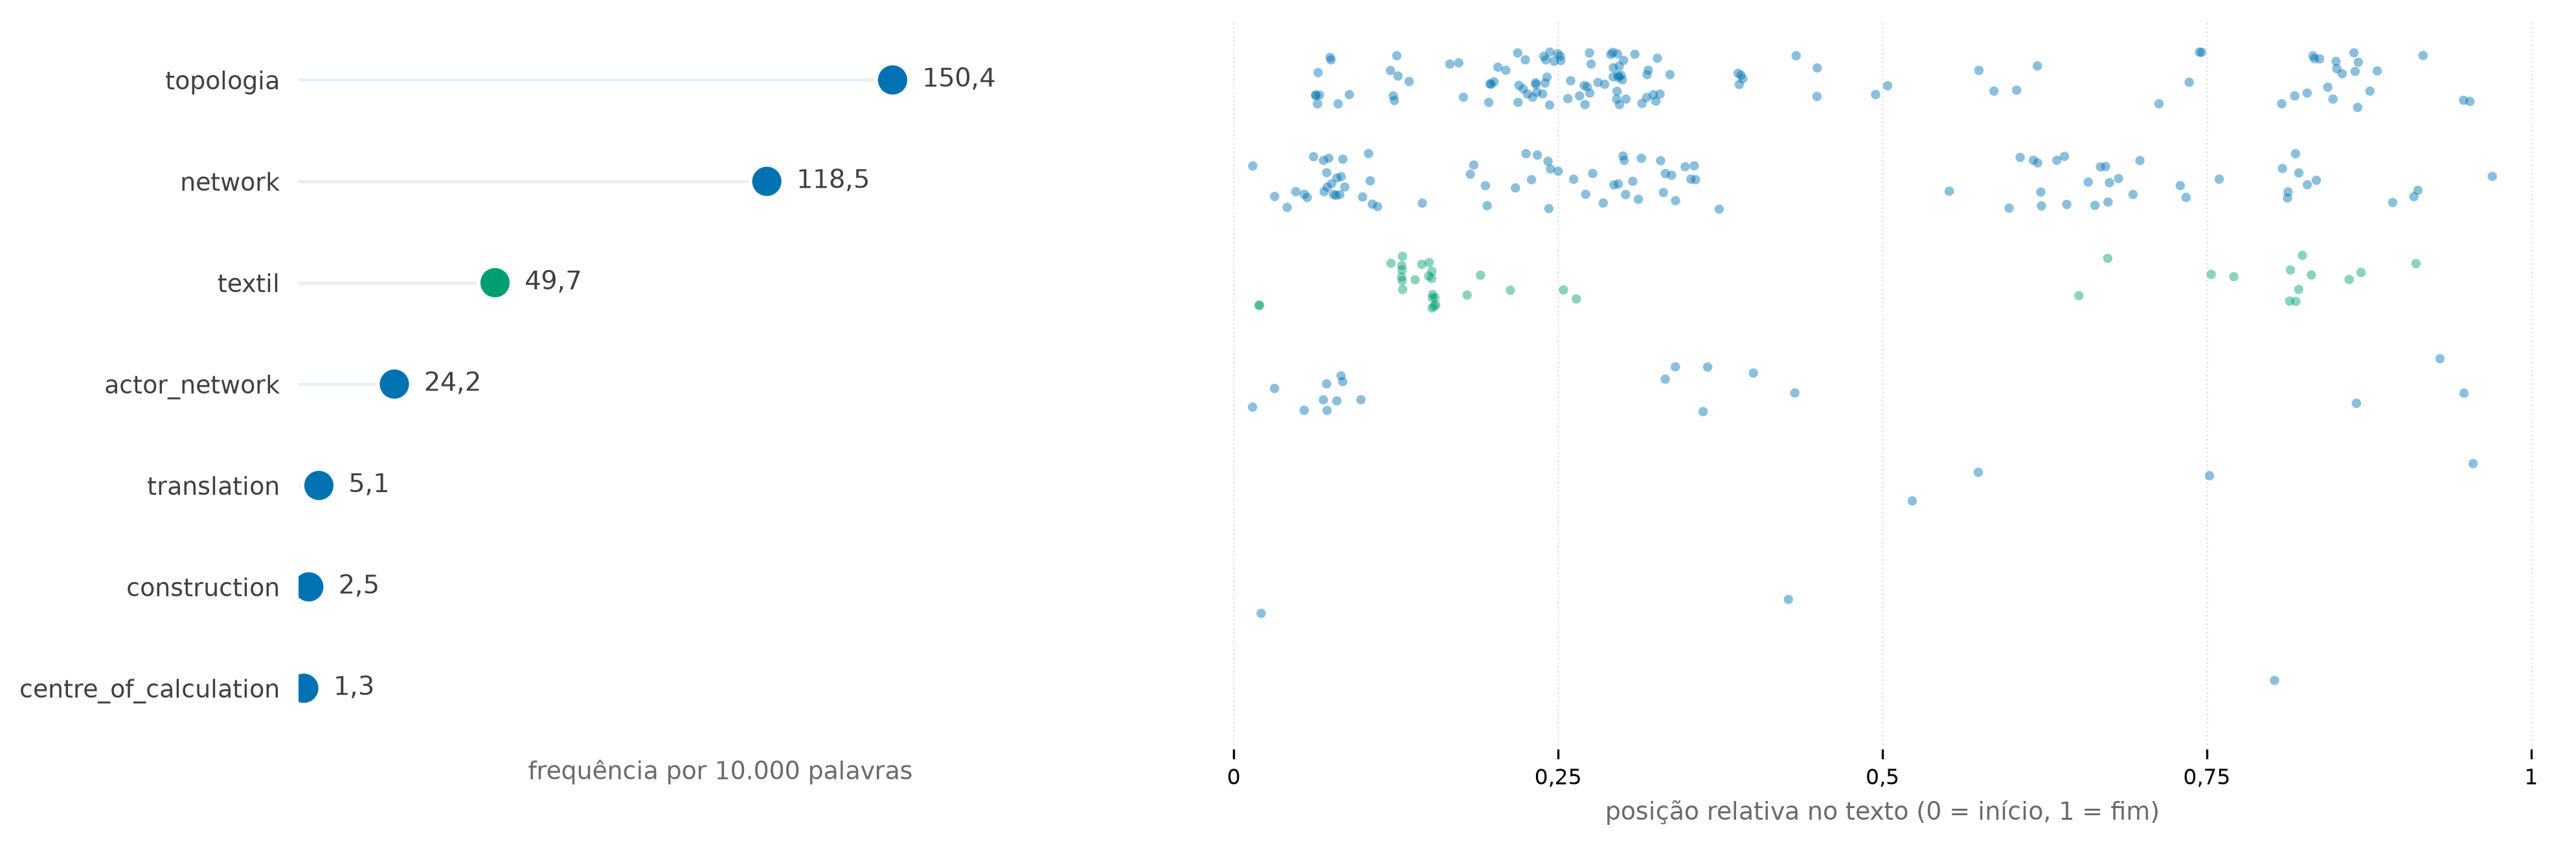
\includegraphics[width=1.0\linewidth]{figuras/cap.2/lexicometria/etapa2_clarifications_freq_e_densidade.png}
\caption[Frequência e distribuição dos rótulos em \emph{Clarifications}]{Rótulos do catálogo lexical em \emph{On Actor-Network Theory: A Few Clarifications} (Latour, 1996). À esquerda, a frequência de cada rótulo em ocorrências por dez mil palavras; à direita, a distribuição das ocorrências ao longo do texto. O artigo soma 276 ocorrências catalogadas, número que já desconta as três ocorrências brutas do rótulo \texttt{militar}. Os rótulos \texttt{topologia} e \texttt{network} dominam o artigo. O rótulo \texttt{militar} aparece com densidade zero, porque as suas ocorrências brutas foram classificadas, por leitura figural, em uso não-figurativo, e a barra do rótulo foi zerada na figura. A distribuição ao longo do texto é homogênea, sem picos localizados, em razão da extensão curta do artigo. Fonte: análise das figurações em \url{github.com/julianehelanski/analise-figuracoes-latour}.}
\label{fig:freq_densidade_clarifications}
\end{figure}

Em \emph{On Recalling ANT}, o mesmo deslocamento se confirma, e a Figura~\ref{fig:freq_densidade_recalling} mostra que a frequência dos rótulos no artigo repete o padrão metateórico de \emph{Clarifications}, com \texttt{topologia} e \texttt{network} no topo e o rótulo \texttt{militar} em densidade zero depois da leitura figural das suas ocorrências. Latour formula a teoria ator-rede como teoria \enquote{flat and folded} em que \enquote{there is no change of scale} \parencite[p.~17]{Latour1999RecallingANT}, e abandona o vocabulário das provas de força para descrever o que a teoria é: \enquote{may be the social possesses the bizarre property of not being made of agency and structure at all, but rather of being a \emph{circulating} entity} \parencite[p.~17]{Latour1999RecallingANT}. A circulação substitui a prova de força, o dobramento substitui a mobilização, o plano substitui o campo de batalha. Em outra passagem do mesmo artigo, ao formular a autocrítica sobre a contaminação do vocabulário que mobilizo desde a abertura deste capítulo~\ref{capitulo2}, Latour situa três dos quatro termos canônicos da teoria, \textit{translation}, \textit{alliance} e \textit{obligatory passage point}, em um vocabulário em que o rótulo \texttt{militar} se mistura com o rótulo \texttt{topologia}: \textit{alliance} é militar, \textit{translation} é têxtil-topológica, \textit{obligatory passage point} é topológico, e \textit{association} é o termo neutro que Latour propõe como melhor candidato \parencite[p.~20]{Latour1999RecallingANT}. A mistura é em si empiricamente significativa: o próprio Latour, ao revisar o vocabulário que herdou de \emph{Science in Action}, hesita entre a figuração militar e a têxtil-topológica e propõe substituições que vão na direção desta última.

\begin{figure}[htbp]
\centering
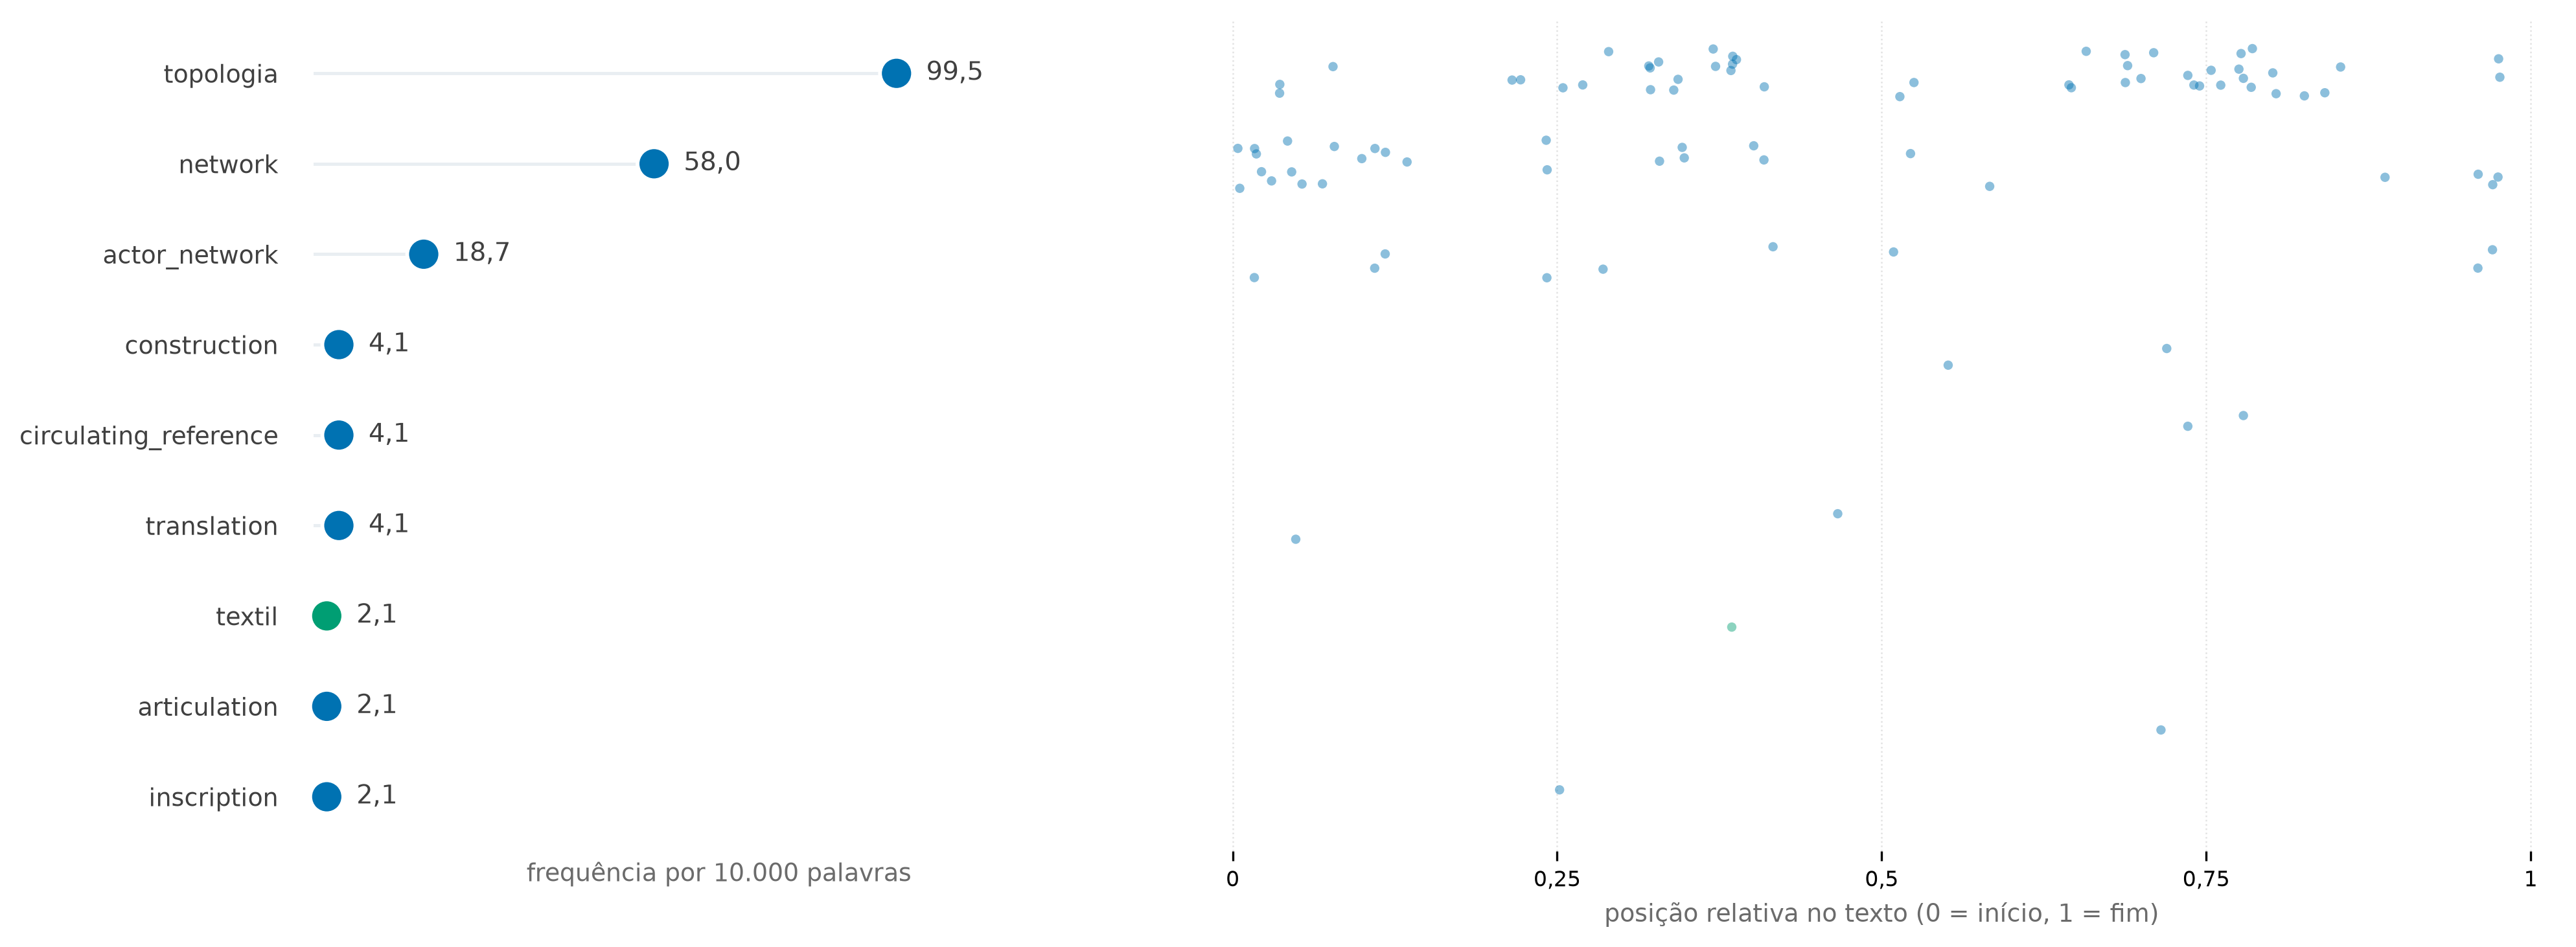
\includegraphics[width=1.0\linewidth]{figuras/cap.2/lexicometria/etapa2bis_recalling_integral_freq_e_densidade.png}
\caption[Frequência e distribuição dos rótulos em \emph{On Recalling ANT}]{Rótulos do catálogo lexical em \emph{On Recalling ANT} (Latour, 1999), sobre o corpus integral da etapa~2-bis. À esquerda, a frequência de cada rótulo em ocorrências por dez mil palavras; à direita, a distribuição das ocorrências ao longo do texto. O número de ocorrências catalogadas exibido no título da figura já desconta as duas ocorrências brutas do rótulo \texttt{militar}. Os rótulos \texttt{topologia} e \texttt{network} dominam o artigo, no mesmo padrão metateórico de \emph{Clarifications}. O rótulo \texttt{militar} aparece com densidade zero, pela mesma leitura figural: as duas ocorrências brutas foram classificadas em uso não-figurativo, e a barra do rótulo foi zerada na figura. A distribuição ao longo do texto é homogênea, sem picos localizados, em razão da extensão curta do artigo. Fonte: análise das figurações em \url{github.com/julianehelanski/analise-figuracoes-latour}.}
\label{fig:freq_densidade_recalling}
\end{figure}

A contagem em densidade relativa, mesmo refinada, ainda mede ocorrências do termo no texto sem distinguir os usos figurais dos usos polissêmicos ou citacionais. Para refinar essa distinção, fiz uma validação amostral semântica sobre as ocorrências dos quatro rótulos centrais nos dois artigos, \texttt{textil}, \texttt{topologia}, \texttt{network} e \texttt{actor\_network}, e classifiquei cada ocorrência amostrada em uso figural, parcialmente figural ou não-figural.\footnote{Fiz a validação amostral em três camadas: cinco ocorrências por rótulo com a janela KWIC mais densa em termos do mesmo rótulo, cinco ocorrências aleatórias por rótulo com semente fixa, e cinco ocorrências por rótulo cuja variante exata é das menos frequentes. Para rótulos com menos de quinze ocorrências, a amostra foi exaustiva. A taxa de figuralidade corresponde à fração ponderada de classificações \emph{figural} sobre o total da amostra do rótulo na obra.} Para \emph{Clarifications}, as taxas de figuralidade confirmam que o vocabulário aparece majoritariamente em uso figural, e não em polissemia residual: o rótulo \texttt{textil} tem taxa de 96,7\%, o rótulo \texttt{topologia} de 93,3\%, o rótulo \texttt{actor\_network} de 90\% e o rótulo \texttt{network} de 70\%. A inversão entre o registro militar dos livros monográficos e o registro têxtil-topológico do artigo metateórico sustenta-se, assim, já no plano figural depurado, para além do plano lexical bruto. Para o \emph{Recalling}, no corpus parcial da etapa~2, o refinamento produz um achado mais sutil: o rótulo \texttt{topologia} mantém taxa de figuralidade integral, mas os rótulos \texttt{network} e \texttt{actor\_network} caem de modo acentuado. A queda indica que, no estrato então processável, as ocorrências de \texttt{network} aparecem em registro predominantemente metalinguístico, com Latour citando o termo \enquote{network} para discutir o que ele significa, mais do que mobilizando o termo para descrever uma rede em ação, e que o rótulo \texttt{actor\_network} ali aparece em uso citacional. O que sobrevive ao refinamento no \emph{Recalling} parcial é o vocabulário topológico denotativo, \textit{flat}, \textit{folded}, \textit{scale}, \textit{circulating}, \textit{flow}, \textit{node} e \textit{connection}, que aparece em registro figural pleno e organiza a redescrição da teoria ator-rede que Latour propõe.

O argumento que sustento é o seguinte: a figuração militar-industrial em Latour é uma figuração de registro descritivo, que aparece quando o objeto da descrição é a tecnociência em ação, enquanto a uma figuração têxtil-topológica é figuração de registro metateórico, utilizada quando o objeto da descrição é a teoria que descreve essa tecnociência. A tensão entre os dois registros atravessa a obra, e o próprio Latour alterna entre os dois conjuntos conforme o objeto que descreve. Dentro do gênero metateórico, a validação amostral semântica identifica ainda uma divisão de segundo nível: \emph{Clarifications} se mantém em registro expositivo-figural, com taxa de figuralidade agregada de 0,875, enquanto \emph{On Recalling ANT} se inscreve em registro autocrítico-metalinguístico, com taxa de 0,636, sustentada pela concentração metalinguística em torno do termo \texttt{network} que Latour tematiza para suspender. O que este capítulo propõe para a tese em geral, em coerência com o gesto assumido na abertura deste capítulo~\ref{capitulo2}, é manter ativas essas figurações na escrita que descreve ao mesmo tempo a tecnociência em ação e a teoria que a descreve. O capítulo~\ref{capitulo3}, ao descrever a rede do \texttt{C4AI} e da \texttt{IBM} que recruta aliados e descreve provas de força, se mantém predominantemente pelo figuração militar-industrial. O capítulo~\ref{capitulo1}, em registro reflexivo sobre a minha própria escrita, se mantém predominantemente nas figurações têxteis, trama, costura, retalho, e essa escolha, que não foi intencional, reflete o que identifiquei na análise lexicométrica das obras de Latour: o vocabulário têxtil é o vocabulário do registro metateórico, e é esse o registro de escrita e de descrição em que o capítulo~\ref{capitulo1} se inscreve. O capítulo~\ref{capitulo4} ocupa uma posição distinta dessa. Ele se faz em registro misto, porque mantém o léxico latouriano da cadeia de translação e da inscrição que organiza também o capítulo~\ref{capitulo3}, e ao mesmo tempo descreve a tecnociência do \texttt{Spira} por meio de figurações têxteis e topológicas, fio, nó, conexão, topologia fluida, objeto fracional. Levar essas figurações à descrição de uma prática tecnocientífica, que pelo padrão que identifiquei na obra de Latour pediria o registro militar-industrial, constitui uma experimentação. Por experimentação entendo a tentativa de observar, descrever, interpretar, analisar e propor a tecnociência por um arranjo de figurações diferente do que o campo dos estudos de ciência e tecnologia mobiliza com mais frequência, e a tensão entre o léxico latouriano e as figurações têxteis é uma parte dessa experimentação. O exercício foi difícil, e a dificuldade tem a forma que o próprio Latour reconheceu em \emph{On Recalling ANT}. Ao admitir que o vocabulário da teoria ator-rede contaminou a capacidade de deixar os atores construírem o seu próprio espaço, Latour diagnostica que o problema, para ele, foi um vocabulário \enquote{not poor enough}, pobre mas ainda insuficientemente pobre, e conclui que projetar um espaço para que os atores desdobrem as suas próprias categorias é \enquote{a much harder task than we thought at first} \parencite[p.~20--21]{Latour1999RecallingANT}. No mesmo movimento, Latour recorre a outras figurações para nomear o que a teoria deveria ser, e cita o conceito \enquote{fluid}, de Law e Mol, ao lado de outras imagens de trilha e de coreografia. O próprio Latour, no momento em que reconhece o limite do léxico que construiu, busca figurações novas, e as busca no vocabulário têxtil-topológico que esta tese rastreia. Deixar os actantes falarem por si é mais difícil do que parece, e talvez por isso seja preciso recorrer a novos modos de pensamento e a novas figurações para descrever, analisar e imaginar as práticas tecnocientíficas. Foi essa dificuldade que encontrei ao longo da escrita desta tese, e ela se manifesta de modo peculiar na maneira como a comecei e em cada uma das tramas tecnoetnográficas que desenvolvi, esta do capítulo~\ref{capitulo2} e as dos capítulos~\ref{capitulo3} e~\ref{capitulo4}.

Cabe mencionar, ainda, um achado complementar que se faz em escala menor e que leva o argumento em outra direção. A segunda edição de \emph{Laboratory Life}, de 1986, acrescentou ao texto da primeira edição, de 1979, um \emph{Postscript} em que Latour e Woolgar fazem balanço retrospectivo do construtivismo social e respondem a críticas. A distribuição dos rótulos dentro desse \emph{Postscript} sustenta, em escala intra-obra, o mesmo padrão que o conjunto de cinco obras sustenta em escala maior. O rótulo \texttt{construction} concentra 13,39 ocorrências por dez mil palavras no \emph{Postscript}, densidade próxima do valor de 19,29 que o rótulo registra no livro inteiro, e que faz de \emph{Laboratory Life} a obra do meu corpus com maior densidade desse campo. A presença do construtivismo no \emph{Postscript} não surpreende: o gênero retrospectivo do \emph{Postscript} é o espaço em que Latour e Woolgar defendem a posição construtivista que organizou o livro. O rótulo \texttt{construction} é, em escala menor, o que o vocabulário têxtil-topológico é em escala maior: vocabulário de registro autorreflexivo, mobilizado quando o objeto da descrição muda da prática para a teoria. O achado pequeno sustenta o achado maior: a autorreflexão muda o vocabulário, e o vocabulário muda conforme o registro em que se escreve.

A etapa~2 e a etapa~2-bis entregaram dois resultados que reorganizam as figurações da obra latouriana. O primeiro é a confirmação refinada por desambiguação, co-ocorrência e validação amostral semântica, de que a figuração militar-industrial é uma figuração situada que aparece de modo seletivo conforme o objeto descrito, e que se ausenta onde a descrição neutra a manteria. O segundo é a demonstração de que a metáfora têxtil-topológica, que reconheço como figuração feminista cujo início mais marcante se deu com Haraway e com a tradição que reconstitui essas figurações associadas ao trabalho de mulheres, é figuração que Latour mesmo compõe em seus momentos autorreflexivos, e que coexiste com a figuração militar-industrial. Assim, a tensão entre figurações que organiza este capítulo encontra, a partir da análise textual, evidências de que ela atravessa a obra latouriana de dentro para fora.

O que nos leva, então, à próxima questão: se as figurações que sustentam a teoria ator-rede são limitadas ou mesmo inadequadas, de que modo descrever, explicar e propor a tecnociência --- neste caso, a pesquisa em IA e acerca de sistemas de IA --- sem reiterar os modos de pensamento das figurações do \textit{front}?

\subsection{A figuração em \emph{An Inquiry into Modes of Existence}}
\label{subsec:figuracao_aime}

Encerro a análise lexicométrica com \emph{An Inquiry into Modes of Existence} (\textit{AIME}), obra na qual Latour repensa a teoria ator-rede de um modo inteiramente novo.\footnote{Cito o livro pela tradução de Catherine Porter publicada pela Harvard University Press em 2013 sob o título \emph{An Inquiry into Modes of Existence: An Anthropology of the Moderns} \parencite{Latour2013Inquiry}. O original em francês, \emph{Enquête sur les modes d'existence}, saiu pela La Découverte em 2012, e a tradução brasileira, \emph{Investigação sobre os modos de existência: uma antropologia dos modernos}, em tradução de Alexandre Agabiti Fernandez, foi publicada pela Editora Vozes em 2019 \parencite{Latour2019Investigacao}. A escolha pelo texto em inglês para a análise lexicométrica é coerente com a etapa 1, em que processei originais ou versões anglo-saxônicas de cada obra de Latour, e com a etapa 2, em que processei os artigos em inglês de 1996 e 1999. As legendas em português dos elementos do quadro 1 que apresento adiante são tomadas da tradução de Agabiti Fernandez, e as legendas em inglês das pp.~487--488 da edição da Harvard. A análise integral está documentada em \url{github.com/julianehelanski/analise-figuracoes-latour/blob/main/outputs/etapa3_aime/relatorio_etapa3.md}.} \emph{AIME} é o livro no qual a criatura de Latour sai do caixão. A teoria ator-rede que ele dissera ter enterrado em \textit{On Recalling ANT}, com quatro pregos e uma estaca no coração, retorna em \textbf{AIME} como ponto de partida de uma investigação ampliada, escrita sob a figura ficcional de uma antropóloga que vai a campo entre os Modernos para reconstituir o sistema de valores das sociedades ocidentais \parencite[p.~28]{Latour2013Inquiry}.\footnote{Latour formula a metáfora dos quatro pregos no caixão para criticar os quatro elementos que compõem a expressão \enquote{teoria ator-rede}. As palavras teoria, ator, rede e o hífen que liga as duas últimas são, na sua leitura, os quatro pregos. A palavra rede (\textit{network}) perdeu seu caráter crítico depois da popularização da internet, e passou a significar transporte sem deformação e acesso instantâneo, o oposto do que a TAR pretendia. A palavra ator (\textit{actor}), ligada à palavra rede pelo hífen, deu margem a mal-entendidos como a dicotomia entre agência e estrutura, na qual a TAR tampouco pretendia entrar. A palavra teoria (\textit{theory}) foi outro equívoco: Latour, citando Mike Lynch, escreve que a TAR deveria ter sido chamada de \enquote{ontologia actante-rizoma} (\textit{actant-rhizome ontology}), mas que ele achou a expressão horrível e o acrônimo \texttt{ARO} pior ainda; além disso, a TAR nunca foi \enquote{uma teoria explicativa do social, mas um método para aprender com os próprios atores} \parencite[p.~19]{Latour1999RecallingANT}. O hífen, por fim, é um lembrete infeliz do debate entre agência e estrutura no qual os autores nunca quiseram entrar. Latour declara, então, ter enterrado sua criatura com quatro pregos e uma estaca no coração, ainda que \enquote{algo leve e belo} pudesse emergir como conquista coletiva futura \parencite{Latour1999RecallingANT}.} 

No capítulo 12 do \textbf{AIME}, Latour afirma: \enquote{the actor-network theory, which the present inquiry seeks to complete} \parencite[p.~353]{Latour2013Inquiry}. O AIME não substitui a teoria ator-rede; complementa-a. A formulação que motiva essa extensão aparece no capítulo 1 do livro, em que a antropóloga ficcional que Latour faz seguir o AIME descobre, no movimento mesmo da pesquisa, a limitação que organiza o resto da \emph{Inquiry}: \enquote{networks [net] have a limitation: they do not qualify values} \parencite[p.~35]{Latour2013Inquiry}. Discuti os limites da teoria ator-rede no capítulo~\ref{capitulo1}, por meio da proposição complementar de cortar e costurar redes com Strathern, Barad, Haraway, Costa e Law. Para a análise lexicométrica que faço aqui, a AIME consiste em uma continuação crítica da teoria ator-rede, por isso, inclui essa obra no corpus; e também por partir e repensar a teoria ator-rede nesta tese. 

\subsubsection{O quadro 1 e a metalinguagem da investigação}
\label{subsubsec:aime_quadro1}

Inicio a análise de \textit{An Inquiry into Modes of Existence} retomando o gesto que o próprio Latour realiza ao final da obra \parencite[pp.~487--488]{Latour2013Inquiry}, em que ele reúne em uma tabela o estado da sua investigação em quinze modos e nas cinco perguntas canônicas que cada modo deve responder. A edição brasileira \parencite[pp.~392--393]{Latour2019Investigacao} traz a tabela com o título \emph{quadro 1: Resumo do estado da investigação} e organiza as quinze linhas em cinco grupos: \enquote{Sem quase-objeto e sem quase-sujeito} (reprodução, metamorfose, hábito), \enquote{Quase-objetos} (técnica, ficção, referência), \enquote{Quase-sujeitos} (política, direito, religião), \enquote{Vínculos entre quase-objetos e quase-sujeitos} (apego, organização, moral) e \enquote{Metalinguagem da investigação} (rede, preposição, duplo clique). As cinco perguntas canônicas que organizam as colunas do quadro orientam a obra de Latour: o \emph{hiato} (\emph{hiatus}) é a descontinuidade característica de cada modo, o ponto em que algo se interrompe e precisa ser retomado por outra caminho; a \emph{trajetória} (\emph{trajectory}) é o movimento específico pelo qual cada modo atravessa esse hiato sem suprimi-lo; as \emph{condições de felicidade e infelicidade} (\emph{felicity and infelicity conditions}) são os critérios que distinguem, em cada modo, o uso bem-sucedido do uso mal-sucedido, e que Latour adota da teoria dos atos de fala de J. L. Austin para qualificar os valores que a rede sozinha não distinguiria; os \emph{seres a instaurar} (\emph{beings to institute}) são as entidades que cada modo faz existir quando a sua trajetória se cumpre; e a \emph{alteração} (\emph{alteration}) é a forma de ser-outro que cada modo institui, em coerência com a tese ontológica do livro de que existir é, sempre, ser-outro de algum modo. O Grupo~5, \emph{Metalinguagem da investigação}, ressoa com a questão da figuração: nesse grupo Latour situa o \enquote{modo rede} ao lado da \enquote{preposição} e do \enquote{duplo clique}, e é esse deslocamento que direciona a análise que faço nesta subseção. A tabela~\ref{tab:aime_quadro1_grupo5} reproduz esse grupo.

\begin{table}[!htb]
\centering
\caption[Grupo 5 do quadro 1 de AIME: a metalinguagem da investigação]{Grupo~5 do quadro~1 de \emph{An Inquiry into Modes of Existence} \parencite{Latour2013Inquiry}: três modos cuja função é dar conta da própria investigação. As seis colunas seguem o quadro~1: o nome do modo e as cinco perguntas canônicas a que cada modo responde. Transcrição minha da edição inglesa, sobre a qual fiz a análise lexicométrica.}
\label{tab:aime_quadro1_grupo5}
\footnotesize
\begin{tabular}{p{1.4cm}p{1.9cm}p{2.0cm}p{2.6cm}p{1.9cm}p{2.0cm}}
\toprule
Name & Hiatus & Trajectory & Felicity and infelicity conditions & Beings to institute & Alteration \\
\midrule
\texttt{[NET]} network & Surprise of association & Following heterogeneous connections & Traverse domains / lose freedom of inquiry & Networks of irreductions & Extend associations \\
\addlinespace
\texttt{[PRE]} preposition & Category mistakes & Detection of crossings & Give each mode its template / crush the modes & Interpretive keys & Ensure ontological pluralism \\
\addlinespace
\texttt{[DC]} double click & Horror of hiatuses & Displacement without translation & Speak literally / speak through figures and tropes & Reign of indisputable Reason & Maintain the same despite the other \\
\bottomrule
\end{tabular}
\end{table}

A teoria ator-rede, que Latour designa pela sigla \texttt{[NET]} em inglês e \texttt{[RES]} em português, e que organizou a descrição da prática tecnocientífica nos três livros e nos dois artigos metateóricos analisados na primeira etapa da análise lexicométrica, aparece em \textit{AIME} sob nova função, como uma das três formas da \enquote{metalinguagem da investigação} (\textit{metalanguage}) que compõem o Grupo 5 do quadro 1.\footnote{O termo \emph{metalanguage} aparece vinte e uma vezes ao longo do corpo de \textit{AIME} em uso teórico pleno. A escolha de não incluir o termo no catálogo da etapa  3 segue o critério que rege esta etapa: o catálogo rastreia o vocabulário figurativo identificado pela leitura qualitativa de \textit{AIME}, e não os rótulos dos grupos que organizam o quadro 1. Registro a presença lexical do termo como observação que abre caminho para uma ampliação futura do catálogo.} A oposição entre \emph{metalanguage} e \emph{infralanguage}, com que Latour qualifica essa metalinguagem, já havia sido estabilizada em \emph{On Actor-Network Theory: A Few Clarifications}, em que Latour escreve que o vocabulário da TAR é \enquote{more an infralanguage than a metalanguage} e que essa infralinguagem \enquote{has to be poor, limited, short and simple} \parencite[p.~\texttt{[p. 7]}]{latour1996clarifications}. Em \textit{AIME}, a oposição se mantém em termos semelhantes: Latour descreve a preposição como \enquote{a metalanguage for this inquiry --- or, better, an infralanguage} \parencite[p.~263]{Latour2013Inquiry}, e prefere \enquote{infralinguagem} porque \enquote{metalinguagem} sugere posição superior ou externa, enquanto a preposição se exerce de dentro da investigação, não de fora. O que muda entre o artigo e o \textit{AIME} é a função que a infralinguagem desempenha: em \emph{Clarifications} ela é a própria TAR como vocabulário pobre que se aplica de modo simétrico a todas as redes; em \textit{AIME} ela passa à preposição \texttt{[PRE]}, e a rede se torna ferramenta empírica, que Latour caracteriza no capítulo 1 do livro como \enquote{a tool that makes a positive empirical investigation possible} \parencite[p.~36]{Latour2013Inquiry} e que ganha estatuto metalinguístico no Grupo 5 ao deixar de ser modo descritivo. O terceiro modo do Grupo 5, o duplo clique \texttt{[DC]}, diz respeito à pretensão de uma metalinguagem universal que aboliria as descontinuidades entre os modos, e que Latour identifica como o adversário a desfazer. Os três modos ocupam, em consequência, lugares distintos: a preposição como infralinguagem por excelência, a rede como ferramenta empírica que ganha estatuto metalinguístico no \textit{AIME} ao deixar de ser modo descritivo, e o duplo clique como pretensão a recusar. O que motiva esse rearranjo é nomeado por Latour no capítulo 1 do \textit{AIME}, em que ele escreve que \enquote{networks have a limitation: they do not qualify values} \parencite[p.~35]{Latour2013Inquiry}: o vocabulário da rede registra as associações sem qualificá-las, e a investigação em modos de existência precisa de outro vocabulário para fazer essa qualificação. Esse outro vocabulário, que Latour distribui ao longo do livro inteiro e sistematiza retrospectivamente no quadro 1 e na Conclusão, é o que a leitura qualitativa que fiz de \textit{AIME} buscou capturar para construir o catálogo novo da etapa  3.\footnote{O catálogo novo da etapa  3 rastreia o vocabulário figurativo que a leitura qualitativa de \textit{AIME} identifica como específico do livro em relação às cinco obras anteriores, e não a taxonomia dos quinze modos de existência que organiza a arquitetura de \textit{AIME}. Os quinze modos, designados pelas siglas \texttt{[rep]}, \texttt{[met]}, \texttt{[hab]}, \texttt{[tec]}, \texttt{[fic]}, \texttt{[ref]}, \texttt{[pol]}, \texttt{[law]}, \texttt{[rel]}, \texttt{[att]}, \texttt{[org]}, \texttt{[mor]}, \texttt{[net]}, \texttt{[pre]} e \texttt{[dc]}, são a nomenclatura técnica com que Latour estrutura a sua investigação, e a sua exposição cabe à literatura especializada sobre \textit{AIME}, não à pergunta lexicométrica que faço aqui. A relação entre os doze rótulos do catálogo novo e o quadro 1 e a Conclusão de \textit{AIME}, documentada na tabela~\ref{tab:mapeamento_quadro1_catalogo_novo}, é de ancoragem textual retrospectiva, e não de derivação a priori. Os identificadores dos rótulos, assim como os identificadores das tabelas e figuras desta subseção, aparecem em inglês em coerência com o tratamento bilíngue do corpus que justifico na nota acima: os identificadores que reproduzem conceitos cunhados por Latour (\texttt{inscription}, \texttt{black\_box}, \texttt{network}) conservam o nome próprio do conceito, e os identificadores que correspondem a rótulos que eu mesma reuni a partir da leitura do corpus (\texttt{militar}, \texttt{textil}, \texttt{topologia}) são etiquetas analíticas minhas e seguem a forma com que constam no repositório.}

A tabela~\ref{tab:mapeamento_quadro1_catalogo_novo} apresenta o mapeamento entre os doze rótulos do catálogo novo e os elementos do quadro 1 e da Conclusão de \textit{AIME} em que cada rótulo encontra ancoragem textual. A correspondência é direta para a maior parte dos rótulos, e nos casos em que ela não é literal indico em coluna própria a passagem do livro em que cada rótulo se sustenta.

\begin{table}[!htb]
\centering
\caption[Mapeamento entre o catálogo novo da etapa  3 e o quadro 1 de AIME]{Mapeamento entre os doze rótulos do catálogo novo da etapa  3 da minha análise lexicométrica e os elementos do quadro 1 e da Conclusão de \textit{AIME} (\textcite{Latour2013Inquiry}, pp.~487--488; tradução brasileira em \textcite{Latour2019Investigacao}) em que cada rótulo encontra ancoragem textual. As três últimas linhas correspondem a vocabulários da Conclusão de \textit{AIME}, fora do quadro 1; as demais correspondem a colunas ou linhas do quadro. A coluna \enquote{ancoragem textual} indica a passagem do livro em que cada rótulo se sustenta, e foi conferida pela leitura do texto integral e pela validação cruzada com as ocorrências do KWIC. Fonte: elaboração própria a partir da leitura qualitativa de \textit{AIME} e da literatura sobre a guinada latouriana pós-2007, com ancoragem retrospectiva no quadro 1 e na Conclusão do livro. Análise lexicométrica documentada em \url{github.com/julianehelanski/analise-figuracoes-latour}.}
\label{tab:mapeamento_quadro1_catalogo_novo}
\small
\begin{tabular}{p{3.8cm}p{3.5cm}p{6.3cm}}
\toprule
Termo de Latour & Campo do catálogo novo & Ancoragem textual em \textit{AIME} \\
\midrule
\emph{Hiatus}                                  & \texttt{trajectory\_pass}     & coluna 2 do Quadro 1; cap.~1 sobre descontinuidades \\
\emph{Trajectory}                              & \texttt{trajectory\_pass}     & coluna 3 do Quadro 1; cap.~2 sobre \enquote{passes} \\
\emph{Felicity and infelicity conditions}      & \texttt{felicity}             & coluna 4 do Quadro 1; cap.~3 sobre condições de veridição \\
\emph{Beings to institute}                     & \texttt{institution}          & coluna 5 do Quadro 1; cap.~2 sobre instituição \\
\emph{Alteration}                              & \texttt{alteration}           & coluna 6 do Quadro 1; cap.~6 sobre ser-enquanto-outro \\
\emph{Name} (modo)                             & \texttt{modes\_of\_existence} & colunas 1 e 7 do Quadro 1; subtítulo do livro \\
\emph{Category mistake} / \emph{domain}        & \texttt{domain\_category}     & cap.~2 sobre o método dos cruzamentos; cap.~1 sobre domínios \\
\emph{The Moderns}                             & \texttt{moderns}              & subtítulo do livro; cap.~1 sobre a antropologia dos modernos \\
\texttt{[PRE]} \emph{preposition} (Grupo 5)    & \texttt{preposition}          & linha 14 do Quadro 1; cap.~3 sobre chaves interpretativas \\
\emph{Negotiation over values} (Conclusão)     & \texttt{values}               & cap.~16 e Conclusão; cap.~9 sobre apego \\
\emph{Diplomatic arrangement} (Conclusão)      & \texttt{diplomacy}            & Conclusão; cap.~14 sobre o cosmos \\
\emph{Gaia} (Conclusão)                        & \texttt{gaia}                 & Conclusão e cap.~16 sobre a era do Antropoceno \\
\bottomrule
\end{tabular}
\end{table}

O mapeamento da tabela~\ref{tab:mapeamento_quadro1_catalogo_novo} sustenta o catálogo novo da etapa  3 em dois apoios independentes: a leitura qualitativa que identifica os rótulos a partir das ocorrências no texto, e o vocabulário que o próprio Latour estabilizou no quadro 1 e na Conclusão de \textit{AIME}. A coincidência entre a leitura e os elementos catalogados por Latour confirma que o vocabulário identificado pela leitura corresponde ao que o livro sistematiza retrospectivamente nas suas duas estruturas de fechamento.

O mapeamento esclarece também a posição do rótulo \texttt{network} do catálogo antigo na análise que apresento a seguir. As 255 ocorrências do rótulo \texttt{network} em \textit{AIME}, em densidade comparável à dos livros da etapa 1, sustentam uma continuidade lexical que oculta uma descontinuidade de função: a rede que em \emph{Science in Action} compunha a gramática descritiva da prática tecnocientífica é, em \textit{AIME}, um instrumento da antropóloga ficcional para detectar as associações heterogêneas entre os modos. O Grupo 5 do quadro 1 torna essa descontinuidade visível, ao situar a rede ao lado da preposição e do duplo clique, no grupo dos modos que dão conta da própria investigação, e não no grupo dos modos descritivos. A análise das tabelas seguintes mede a continuidade lexical do termo, e a leitura interpretativa que faço dessas tabelas reconhece a descontinuidade de função que está por trás dela.

Sigo, em consequência, dois catálogos aplicados em paralelo na análise de \textit{AIME}. O primeiro é o catálogo de dezenove rótulos das etapas 1 e 2, que aplico a \textit{AIME} para permitir a comparação direta com as cinco obras anteriores. O segundo é o catálogo de doze rótulos da etapa 3, que construí a partir da leitura qualitativa de \textit{AIME} e da literatura sobre a obra tardia de Latour, e que encontra ancoragem retrospectiva no quadro 1 e na conclusão do livro conforme a tabela~\ref{tab:mapeamento_quadro1_catalogo_novo}. A construção do catálogo novo exigiu algumas decisões de depuração, porque vários dos termos que apareciam na leitura têm na língua inglesa usos polissêmicos: \emph{value} pode ser axiológico ou econômico, \emph{mode} pode ser nome técnico ou substantivo comum, \emph{modern} pode ser adjetivo descritivo ou nome próprio dos modernos, \emph{Earth} pode ser planeta ou solo fértil. Cada um desses termos passou por uma decisão de inclusão ou exclusão, que privilegia as expressões em que Latour usa o termo em sentido técnico próprio do livro.\footnote{As decisões pontuais de depuração de cada rótulo, com as variantes mantidas e as variantes retiradas, estão registradas no arquivo \texttt{campos\_lexicais/catalogo\_termos\_aime.yaml} do repositório, em \url{github.com/julianehelanski/analise-figuracoes-latour}. A polissemia residual dos termos \emph{experience}, \emph{crossing}, \emph{domain} e \emph{value} carrega ruído que a contagem bruta reflete, e a leitura interpretativa precisa considerá-lo. A aplicação do catálogo novo apenas a \textit{AIME}, e não retroativamente às cinco obras anteriores, decorre da origem do catálogo: os doze rótulos correspondem a vocabulário específico de \textit{AIME} identificado pela leitura qualitativa, e o rendimento esperado da aplicação retroativa nos textos de 1986 a 1999 seria de ordem de grandeza inferior ao ruído.} O corpus de \textit{AIME} passou pelas mesmas etapas de saneamento que apliquei às outras obras, descritas em detalhe no repositório.

\begin{longtable}{@{}p{0.23\textwidth} p{0.23\textwidth} p{0.46\textwidth}@{}}
\caption[Catálogo lexical da etapa 3 (AIME)]{Catálogo lexical da etapa 3 (\textit{AIME}, 2013): os doze rótulos identificados pela leitura qualitativa do livro e da literatura sobre a obra tardia de Latour, com a ancoragem textual de cada campo no quadro 1 e na conclusão de \textit{AIME} e uma amostra dos termos que o definem. A amostra segue a ordem do arquivo de definição: rótulos com até oito termos aparecem completos, rótulos maiores trazem os oito primeiros termos seguidos de \enquote{entre outros}. A lista completa está no repositório, em \texttt{campos\_lexicais/catalogo\_termos\_aime.yaml}, em \url{github.com/julianehelanski/analise-figuracoes-latour}.}\label{tab:catalogo-etapa3}\\
\toprule
Campo & Ancoragem textual em \textit{AIME} & Amostra de termos do catálogo \\
\midrule
\endfirsthead
\caption[]{Catálogo lexical da etapa  3 (\textit{AIME}) (continuação).}\\
\toprule
Campo & Ancoragem textual em \textit{AIME} & Amostra de termos do catálogo \\
\midrule
\endhead
\midrule
\multicolumn{3}{r@{}}{\footnotesize continua na próxima página}\\
\endfoot
\bottomrule
\endlastfoot
\texttt{modes\_of\_existence} & Quadro 1 / Conclusão & \texttt{mode of existence}, \texttt{modes of existence} \\
\texttt{preposition} & Quadro 1 / Conclusão & \texttt{preposition}, \texttt{prepositions}, \texttt{prepositional} \\
\texttt{felicity} & Quadro 1 / Conclusão & \texttt{felicity}, \texttt{infelicity}, \texttt{felicity condition}, \texttt{infelicity condition}, \texttt{felicity conditions}, \texttt{infelicity conditions}, \texttt{felicitous}, \texttt{infelicitous} \\
\texttt{diplomacy} & Quadro 1 / Conclusão & \texttt{diplomatic}, \texttt{diplomat}, \texttt{diplomats}, \texttt{diplomacy}, \texttt{negotiation}, \texttt{negotiations}, \texttt{negotiating}, \texttt{negotiate}, entre outros \\
\texttt{gaia} & Quadro 1 / Conclusão & \texttt{Gaia}, \texttt{Anthropocene}, \texttt{terrestrial}, \texttt{ecology}, \texttt{ecological}, \texttt{ecologies}, \texttt{climate}, \texttt{climatologist}, entre outros \\
\texttt{values} & Quadro 1 / Conclusão & \texttt{qualify values}, \texttt{qualifies values}, \texttt{qualifying values}, \texttt{qualified values}, \texttt{value system}, \texttt{values system}, \texttt{system of values}, \texttt{qualify} \\
\texttt{trajectory\_pass} & Quadro 1 / Conclusão & \texttt{trajectory}, \texttt{trajectories}, \texttt{course of action}, \texttt{hiatus}, \texttt{discontinuity}, \texttt{discontinuities}, \texttt{continuity}, \texttt{continuities}, entre outros \\
\texttt{institution} & Quadro 1 / Conclusão & \texttt{instituting}, \texttt{institute}, \texttt{institutes}, \texttt{instituted}, \texttt{institution}, \texttt{institutions} \\
\texttt{domain\_category} & Quadro 1 / Conclusão & \texttt{category mistake}, \texttt{category mistakes}, \texttt{domain}, \texttt{domains}, \texttt{crossing}, \texttt{crossings} \\
\texttt{moderns} & Quadro 1 / Conclusão & \texttt{Moderns}, \texttt{modernity}, \texttt{modernizing}, \texttt{modernism}, \texttt{modernization} \\
\texttt{alteration} & Quadro 1 / Conclusão & \texttt{alteration}, \texttt{alterations}, \texttt{alter}, \texttt{altered}, \texttt{alters}, \texttt{altering}, \texttt{being-as-other}, \texttt{being-as-another}, entre outros \\
\texttt{experience} & Quadro 1 / Conclusão & \texttt{experience}, \texttt{experiences}, \texttt{experienced}, \texttt{experiential}, \texttt{empirical} \\
\end{longtable}

A contagem do catálogo das etapas 1 e 2 aplicada a \textit{AIME} sustenta dois achados que articulo em sequência. O primeiro é a continuidade do vocabulário têxtil-topológico em densidade intermediária, com reorganização lexical interna. A densidade do rótulo \texttt{topologia} em \textit{AIME} (26,43 por dez mil palavras) coloca a obra no mesmo patamar de \emph{Science in Action} (34,68) e \emph{Pandora's Hope} (27,58), abaixo das densidades extraordinárias dos artigos, em parte inflacionadas pela tamanho menor do corpus em que aparecem. Em valor absoluto, \textit{AIME} registra 514 ocorrências do rótulo \texttt{topologia}, número maior do que em qualquer das obras anteriores, e o livro mobiliza o vocabulário topológico em volume que faz dele o rótulo mais denso da obra inteira. As variantes \emph{top} do rótulo \texttt{topologia} em \textit{AIME} são \emph{path} (90), \emph{trajectory} (61), \emph{outside} (55), \emph{trajectories} (34) e \emph{paths} (33), em diferença com \emph{Science in Action} e \emph{Pandora's Hope}, em que dominavam \emph{inside}, \emph{outside}, \emph{scale} e \emph{flow}. O vocabulário topológico em \textit{AIME} se reorganiza em torno do par \emph{path}/\emph{trajectory}, que se articula com o rótulo novo \texttt{trajectory\_pass} que apresento adiante. O rótulo \texttt{network} em \textit{AIME} (13,11 por dez mil palavras) é o mais alto entre as obras do corpus, superando os 4,26 de \emph{Laboratory Life}, os 9,08 de \emph{Science in Action} e os 2,73 de \emph{Pandora's Hope}, e fica em ordem de grandeza intermediária entre os livros e os artigos metateóricos. O rótulo \texttt{textil} em \textit{AIME} (10,34 por dez mil) registra densidade comparável à dos livros (7,94 e 8,20). O vocabulário têxtil-topológico permanece em \textit{AIME}, portanto, em densidade intermediária, sem o pico dos artigos metateóricos e sem o recuo que se poderia esperar caso Latour tivesse abandonado esse vocabulário ao virar a página em direção aos modos de existência.

O segundo achado é a reentrada moderada do vocabulário militar bruto em \textit{AIME}, em densidade reduzida em relação aos livros monográficos solo. A contagem do rótulo \texttt{militar} é de 6,63 por dez mil palavras (129 ocorrências em 194.454 palavras de corpo), em patamar intermediário entre a dos artigos metateóricos (3,82 em \emph{Clarifications}, 4,15 em \emph{Recalling ANT}) e a dos livros monográficos solo (16,56 em \emph{Pandora's Hope}, 26,74 em \emph{Science in Action}).\footnote{A contagem aqui é bruta. A desambiguação refinada do rótulo \texttt{militar} foi aplicada aos três livros das etapa s 1 e 2 e aos dois artigos da etapa  2, e separa, dentro do rótulo, as ocorrências de tropo figural latouriano das ocorrências de uso bibliográfico, metalinguístico, descritivo-histórico ou de polêmica conceitual. A aplicação da desambiguação refinada às 129 ocorrências do rótulo \texttt{militar} em \textit{AIME} fica como pendência da pesquisa, em coerência com o critério da etapa  3 de não incluir validação amostral semântica nesta passagem do trabalho (declaração registrada em \texttt{outputs/etapa3\_aime/relatorio\_etapa3.md} no repositório público).} As variantes \emph{top} do rótulo \texttt{militar} em \textit{AIME} são \emph{war} (22), \emph{mobilizing} (20), \emph{defend} (12), \emph{enemies} (9) e \emph{wars} (7). A leitura qualitativa dessas ocorrências mostra que o vocabulário militar aparece em \textit{AIME} em registro deslocado em relação ao dos livros monográficos solo: onde \emph{Science in Action} mobilizava \emph{ally}, \emph{mobilise}, \emph{enroll} e \emph{battle} para descrever a prática científica como tal, \textit{AIME} mobiliza o mesmo vocabulário em torno de objetos cosmopolítico-diplomáticos. O título do capítulo 14 do livro é \enquote{Mobilizing the Beings of Passionate Interest} (modo \texttt{[ATT]}, da atração econômica), e ocorrências como \enquote{battles have ceased for want of combatants} ou \enquote{for new wars a new peace} se inscrevem em registro que articula o vocabulário militar à cena diplomática que o livro inaugura. O vocabulário militar volta, em densidade reduzida, e o objeto militarmente descrito muda do laboratório e da controvérsia à cosmopolítica e à diplomacia. A co-ocorrência do rótulo \texttt{militar} com os rótulos do catálogo novo confirma esse deslocamento: \texttt{militar}--\texttt{moderns} aparece em 144 co-ocorrências na janela de duzentas palavras, \texttt{militar}--\texttt{institution} em 78, \texttt{militar}--\texttt{diplomacy} em 55, e \texttt{militar}--\texttt{gaia} em 45. O vocabulário militar em \textit{AIME} se articula com o vocabulário cosmopolítico-diplomático novo, e se afasta do vocabulário da prova de força e do alistamento que dominava \emph{Science in Action}.

A tabela~\ref{tab:aime_catalogo_novo} apresenta a contagem dos doze rótulos novos identificados em \textit{AIME}.

\begin{table}[!htb]
\centering
\caption[Doze rótulos novos identificados em AIME 2013]{Densidade dos doze rótulos novos identificados em \textit{AIME} (2013) e aplicados apenas nesta obra. Ocorrências por dez mil palavras em 194.454 palavras de corpo; contagem absoluta entre parênteses. Fonte: etapa  3 da análise lexicométrica em \url{github.com/julianehelanski/analise-figuracoes-latour}. Catálogo novo identificado pela leitura qualitativa de \textit{AIME} e aplicado apenas nesta obra. As variantes \emph{top} de cada rótulo estão documentadas no relatório da etapa  3.}
\label{tab:aime_catalogo_novo}
\small
\begin{tabular}{lrr}
\toprule
Campo & $n$ & freq./10k \\
\midrule
trajectory\_pass    & 433 & 22{,}27 \\
moderns             & 397 & 20{,}42 \\
domain\_category    & 281 & 14{,}45 \\
experience          & 276 & 14{,}19 \\
institution         & 227 & 11{,}67 \\
modes\_of\_existence & 167 &  8{,}59 \\
alteration          & 112 &  5{,}76 \\
felicity            &  92 &  4{,}73 \\
diplomacy           &  84 &  4{,}32 \\
preposition         &  71 &  3{,}65 \\
gaia                &  52 &  2{,}67 \\
values              &  22 &  1{,}13 \\
\midrule
\textit{Total}      & \textit{2.214} & \textit{113{,}86} \\
\bottomrule
\end{tabular}
\end{table}

A tabela~\ref{tab:aime_catalogo_novo} apresenta o catálogo novo da etapa 3 aplicado a \textit{AIME}, com os doze rótulos em ordem decrescente de frequência. A figura~\ref{fig:aime_freq_densidade} amplia o quadro, mostra os dois catálogos aplicados em paralelo a \textit{AIME}, em duas perspectivas. À esquerda, mostra quanto cada rótulo aparece em \textit{AIME}, com os rótulos do catálogo antigo em uma cor e os do catálogo novo em outra, o que torna visível a justaposição entre os dois vocabulários. À direita, mostra onde, ao longo do livro, cada rótulo se concentra ou se distribui, do início ao fim das 194.454 palavras de \textit{AIME}.

\begin{figure}[htbp]
\centering
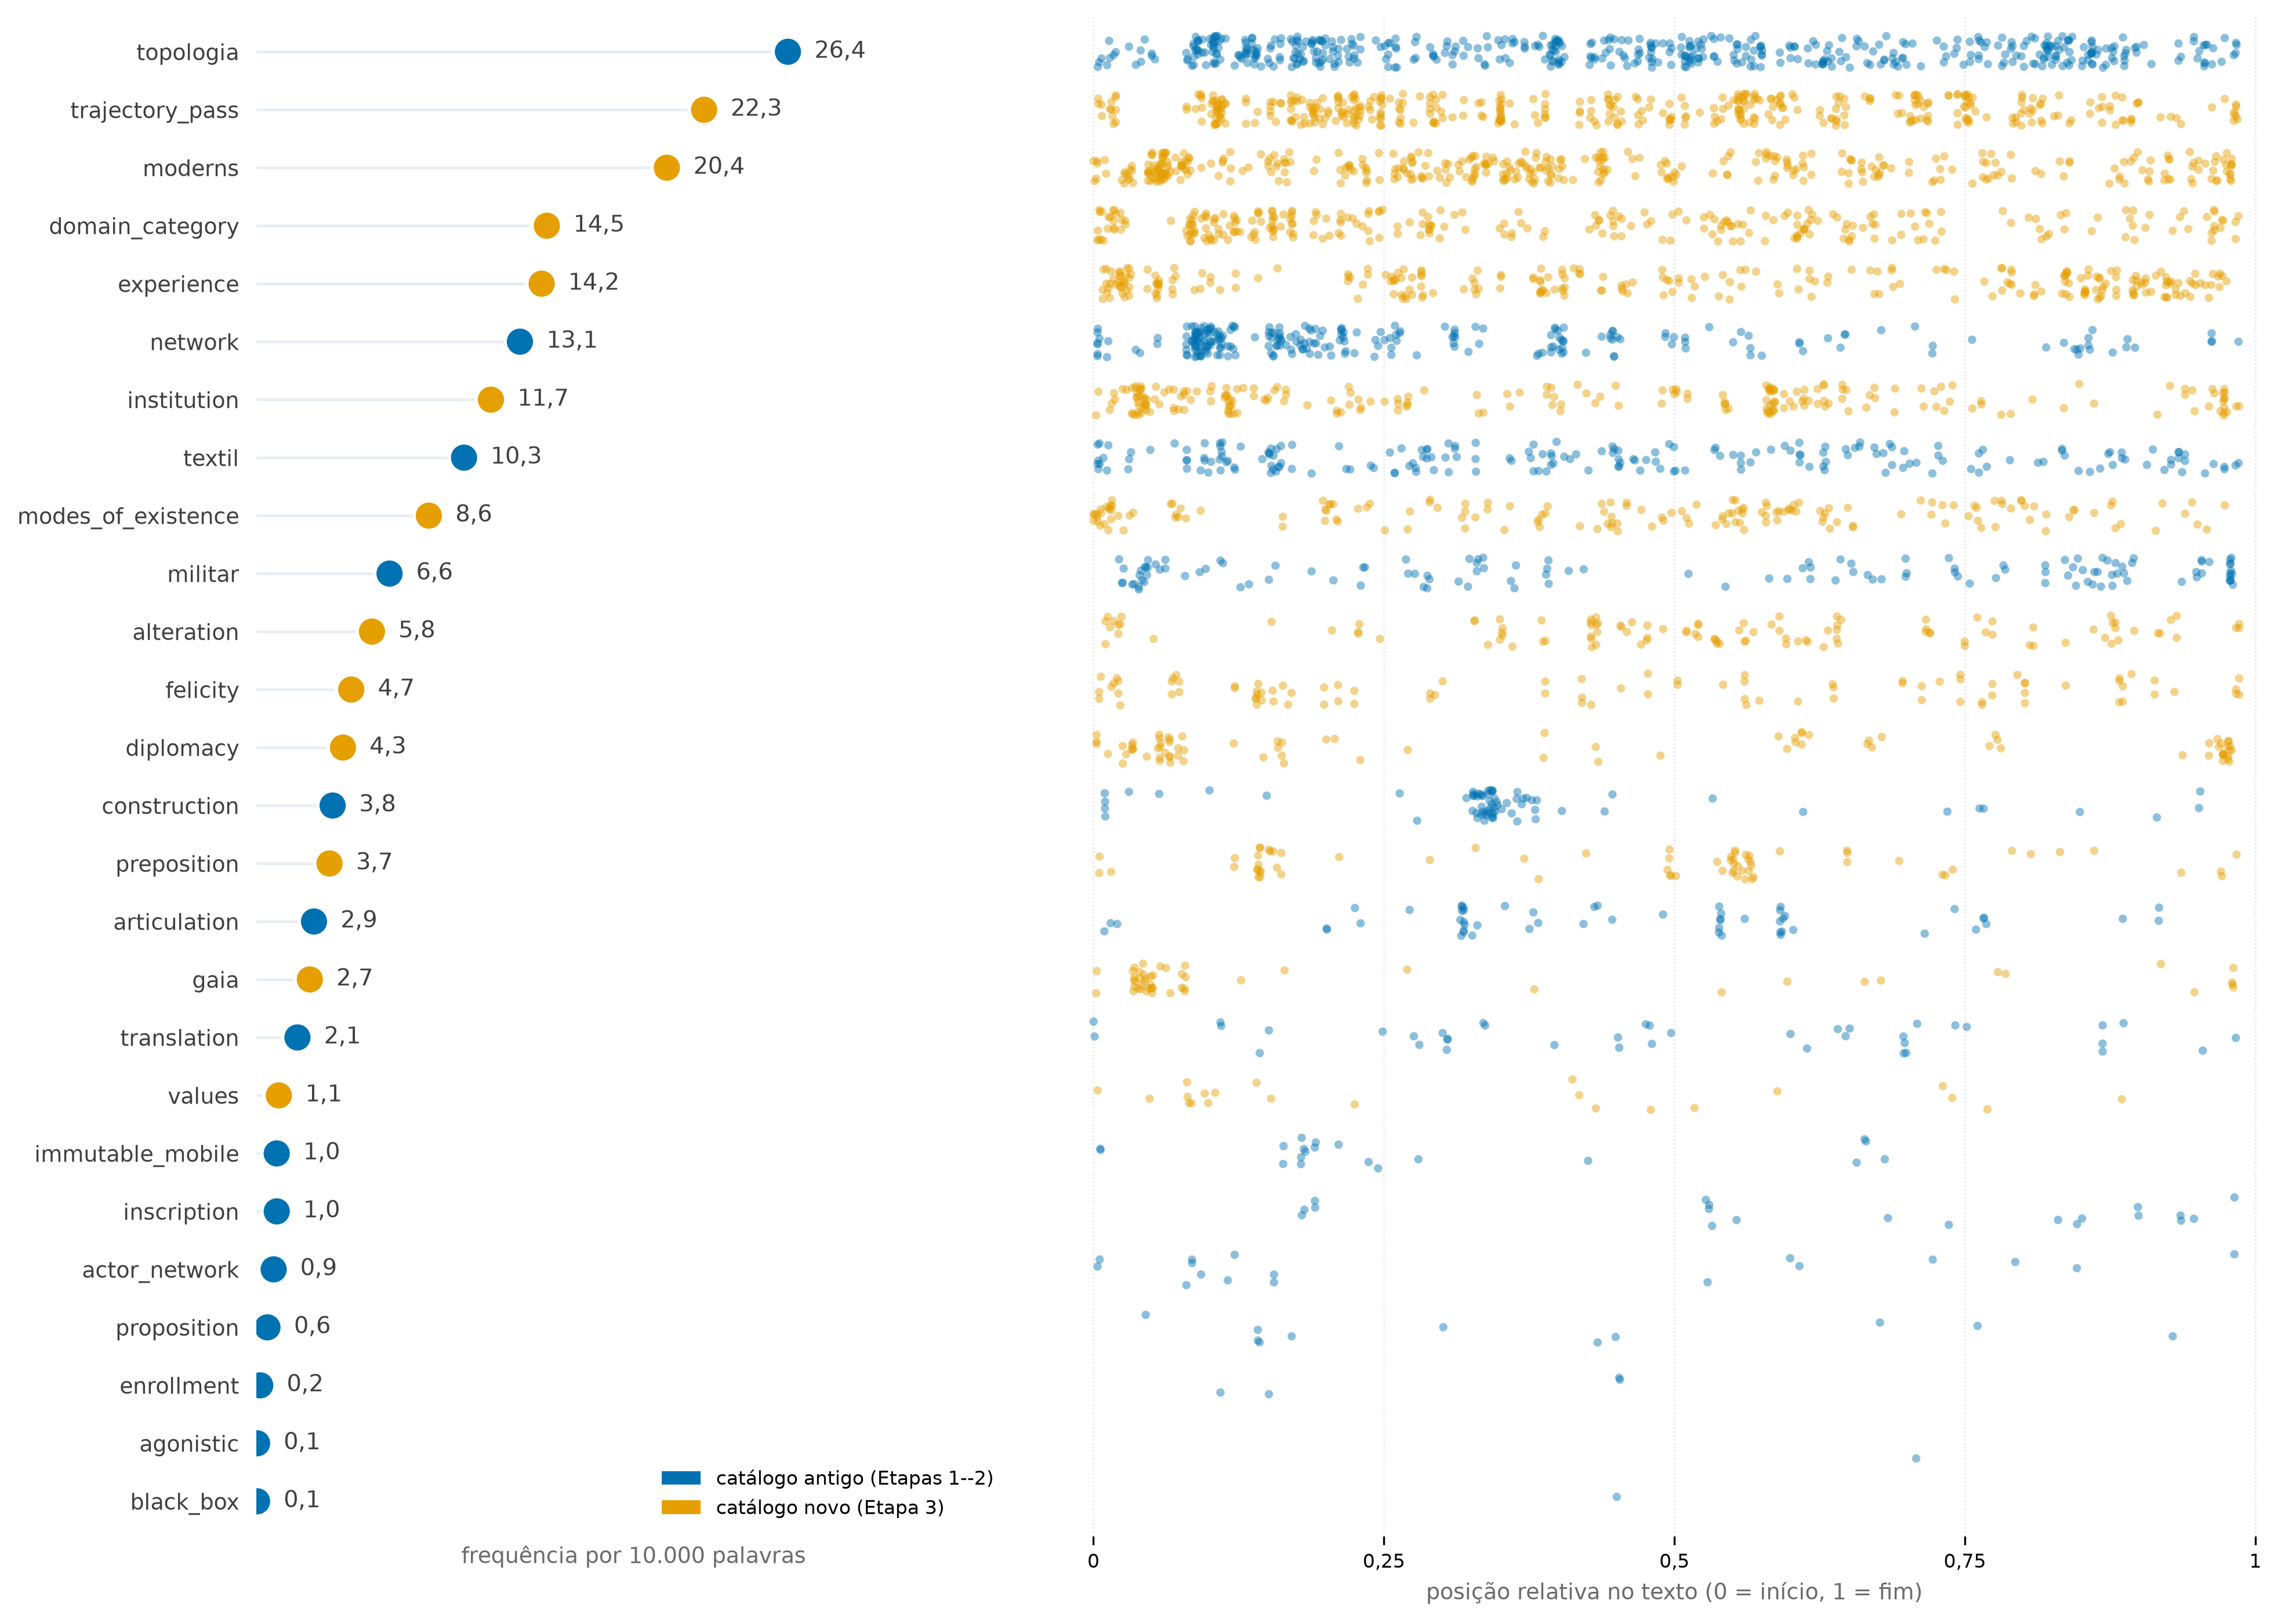
\includegraphics[width=1.0\linewidth]{figuras/cap.2/lexicometria/etapa3_aime_freq_e_densidade.png}
\caption[Frequência e distribuição dos rótulos em AIME]{Frequência e distribuição dos rótulos em \textit{AIME} \parencite{Latour2013Inquiry}. À esquerda, quanto cada um dos vinte e seis rótulos aparece em \textit{AIME}, com duas cores que distinguem o vocabulário figurativo herdado das obras anteriores (em azul) do vocabulário próprio do livro identificado pela leitura qualitativa (em laranja). À direita, onde, ao longo das 194.454 palavras de \textit{AIME}, cada rótulo se concentra ou se distribui, do início ao fim do livro. Soma de 3.557 ocorrências. Os rótulos \texttt{experience} e \texttt{domain\_category} têm alta polissemia em inglês e carregam ruído que a leitura interpretativa precisa considerar. Fonte: análise das figurações em \url{github.com/julianehelanski/analise-figuracoes-latour}.}
\label{fig:aime_freq_densidade}
\end{figure}

A leitura do painel de distribuição registra três regularidades. A primeira: o rótulo \texttt{moderns} aparece em densidade alta e de modo relativamente homogêneo ao longo de todo o livro, em correspondência com a \enquote{antropologia dos modernos} que dá subtítulo à obra. A segunda: \texttt{topologia} e \texttt{trajectory\_pass} concentram densidade alta na primeira metade do livro, na zona dos capítulos introdutórios em que Latour expõe o aparato conceitual dos modos de existência. A terceira: o rótulo \texttt{militar}, décimo na densidade absoluta com 129 ocorrências brutas, distribui-se ao longo do texto sem concentração em capítulo específico, em contraste com o pico inicial que apresentou em \emph{Science in Action} e em \emph{Pandora's Hope}.

O painel registra ainda um movimento de ausência. Cinco rótulos do catálogo antigo zeram em \textit{AIME}: \texttt{centre\_of\_calculation}, \texttt{trial\_of\_strength}, \texttt{factish}, \texttt{circulating\_reference} e \texttt{spokesperson}. Os cinco são neologismos próprios de Latour que ele cunhou ao longo das obras anteriores (\textit{trial of strength} e \textit{centre of calculation} em \emph{Science in Action}; \textit{factish} e \textit{circulating reference} em \emph{Pandora's Hope}; \textit{spokesperson} em \emph{Science in Action}), e o fato de que zeram simultaneamente em livro de 194.454 palavras é dado etnograficamente significativo. O termo \texttt{actor\_network} cai de 24,21 por dez mil em \emph{Clarifications} (1996) para 0,87 em \textit{AIME} (2013), em recuo de mais de vinte e seis vezes. Latour, ao escrever \textit{AIME}, abandona o registro descritivo dos livros e abandona também o vocabulário canônico que ele mesmo cunhou, fazendo com que o \textit{AIME} seja um livro de reformulação sistemática.

A leitura conjunta da tabela~\ref{tab:aime_catalogo_novo} e das figuras anteriores mostra que o vocabulário figurativo herdado das obras anteriores aparece em \textit{AIME} com 1.343 ocorrências distribuídas em dezenove rótulos, ao passo que o vocabulário próprio do livro, aquele que a leitura qualitativa identificou como específico de \textit{AIME}, aparece com 2.214 ocorrências distribuídas em doze rótulos. O vocabulário próprio do livro é, em volume bruto, sessenta e cinco por cento mais denso do que o vocabulário herdado que \textit{AIME} mantém em circulação. A passagem teórica que \textit{AIME} realiza se faz por justaposição entre os dois vocabulários: o livro continua mobilizando o vocabulário da TAR e dos livros monográficos em densidades intermediárias, e acrescenta uma camada figural própria em que predominam \texttt{trajectory\_pass}, \texttt{moderns}, \texttt{domain\_category}, \texttt{experience} e \texttt{institution}. A co-ocorrência entre os rótulos dos dois vocabulários mostra como essa justaposição se organiza: o par mais denso de \textit{AIME}, com 584 co-ocorrências, é \texttt{topologia}--\texttt{trajectory\_pass}, articulação que costura o vocabulário topológico herdado ao vocabulário pragmatista de movimento descontínuo que \textit{AIME} introduz (com variantes \emph{top} \emph{continuity}, \emph{hiatus}, \emph{trajectory} e \emph{discontinuities}).\footnote{Os rótulos \texttt{topologia} e \texttt{trajectory\_pass} compartilham os termos \emph{trajectory} e \emph{trajectories}. Em noventa e cinco posições do texto de \textit{AIME} a mesma ocorrência é contada nos dois rótulos, e essas posições entram como pares de distância nula na contagem de co-ocorrência. A leitura do par como costura entre o vocabulário topológico herdado e o vocabulário pragmatista que \textit{AIME} introduz deve considerar, portanto, que parte da sua densidade decorre dessa partilha de termos, e não apenas da vizinhança textual entre rótulos distintos.} Os pares secundários \texttt{network}--\texttt{topologia} (379 co-ocorrências), \texttt{network}--\texttt{trajectory\_pass} (301), \texttt{domain\_category}--\texttt{topologia} (285) e \texttt{domain\_category}--\texttt{network} (264) sustentam a malha figural integrada do livro.\footnote{A análise de co-ocorrência em \textit{AIME} foi feita em duas configurações de janela de contexto, e o ranking dos dez pares principais se preserva nas duas. A decisão sobre as janelas está documentada em \path{docs/decisoes_metodologicas.md} no repositório público, e a análise é reproduzível pelo procedimento ali versionado.}

O quadro figural de \textit{AIME}, lido nas quatro tabelas e nos pares de co-ocorrência, organiza-se em três camadas. A primeira é a do vocabulário antigo persistente, que \textit{AIME} mantém em densidades intermediárias: \texttt{topologia}, \texttt{network}, \texttt{textil}, \texttt{militar}, \texttt{construction}, \texttt{articulation} e \texttt{translation}. A segunda é a do vocabulário novo pragmatista, próprio do livro, que descreve os modos de existência como tipos de movimento descontínuo qualificados por condições de felicidade próprias: \texttt{trajectory\_pass}, \texttt{experience}, \texttt{alteration}, \texttt{felicity}, \texttt{preposition}, \texttt{modes\_of\_existence} e \texttt{values}. A terceira é a do vocabulário cosmopolítico, em que o livro articula a antropologia dos modernos com a cena diplomática que ele propõe: \texttt{moderns}, \texttt{institution}, \texttt{domain\_category}, \texttt{diplomacy} e \texttt{gaia}. As três camadas se articulam entre si pela co-ocorrência: o vocabulário topológico continuado se costura ao vocabulário pragmatista novo no par \texttt{topologia}--\texttt{trajectory\_pass}, e o vocabulário militar deslocado se costura ao vocabulário cosmopolítico na constelação \texttt{militar}--\texttt{moderns}--\texttt{diplomacy}--\texttt{gaia}.

Explicito o estatuto da análise que apresento nesta subseção, porque ele exige mais cuidado aqui do que em qualquer das obras anteriores. A densidade que registro nas tabelas e nas figuras é medida que se forma no encontro entre o corpus, o catálogo de rótulos que construí para lê-lo e a janela de contexto que defini para contar as ocorrências. Em \textit{AIME} esse encontro tem uma camada a mais, porque a obra é a única do corpus que conto com dois catálogos aplicados em paralelo. A soma de 3.557 ocorrências, e a proporção de sessenta e cinco por cento que separa o volume do catálogo novo do volume do catálogo antigo, são valores que dependem de quantos rótulos compõem cada um dos catálogos e de quais termos reúno em cada rótulo, decisões que tomei na leitura qualitativa de \textit{AIME}. A análise lexicométrica de \textit{AIME} traz ainda uma pendência declarada, uma vez que a desambiguação refinada do rótulo \texttt{militar}, aplicada aos três livros das etapas 1 e 2 e aos dois artigos da etapa 2, não foi aplicada às 129 ocorrências do rótulo \texttt{militar} em \textit{AIME}, e a sua aplicação fica como continuidade do trabalho registrada no repositório. A proporção que leio como o achado central desta subseção sustenta-se enquanto ordem de grandeza, e não como valor exato, pois, o que ela registra que a camada figurativa nova de \textit{AIME} é densa o bastante para rivalizar com a camada herdada, e é dessa forma, o de uma medida co-produzida, que a tomo.

A análise das figurações que sustento neste capítulo~\ref{capitulo2}, organizada pela divisão de trabalho metafórico entre o registro descritivo dos três livros e o registro metateórico dos dois artigos, encontra em \textit{AIME} um terceiro tempo. \textit{AIME} é livro monográfico formalmente, em volume comparável aos livros monográficos solo (194.454 palavras, em ordem de grandeza de \emph{Science in Action} e \emph{Pandora's Hope}), e é livro metateórico em conteúdo, dado que Latour escreve para reformular o vocabulário que ele mesmo cunhou e que orientou cerca de trinta anos de produção. Na análise, identifico que essa posição mista se inscreve no léxico de três maneiras articuladas. A densidade do vocabulário militar em \textit{AIME} é claramente inferior à dos livros, com 6,63 ocorrências por dez mil palavras contra 26,74 em \emph{Science in Action} e 16,56 em \emph{Pandora's Hope}, sem zerar como acontece nos dois artigos. O vocabulário têxtil-topológico permanece em \textit{AIME} em densidade comparável à desses livros, sem o pico que esse vocabulário registra nos artigos. E o vocabulário próprio do livro, aquele que a leitura qualitativa identificou como específico de \textit{AIME}, ocupa o lugar que nas obras anteriores ficava reservado para a descrição da prática tecnocientífica. A guinada das figurações que se desenhava nas obras anteriores, e que esta tese reconstitui através da análise lexicométrica e da leitura situado, fica em \textit{AIME} consolidada como de maneira sistemátia. Latour conserva o vocabulário herdado das obras anteriores, justapõe à elas o vocabulário próprio do livro, e organiza a escrita em três camadas figurativas que articulam a herança da TAR à reformulação dos modos de existência.

A análise das figurações em seis obras de Latour mostra que a tensão entre figuração militar-industrial e figuração têxtil-topológica que organiza esta tese atravessa também a obra latouriana. A figuração militar-industrial, a figuração têxtil-topológica e a figuração cosmopolítico-diplomática coexistem em Latour em densidades que variam por gênero textual, por momento da trajetória e por objeto descrito. Concluo com isso que as três figurações acompanham o movimento de uma escrita que se reescreveu ao longo da produção de Latour, do laboratório de Roger Guillemin em 1979 à investigação sobre os modos de existência dos modernos em 2013.

O repertório que acabo de apresentar não me chegou pronto, e sim por um percurso de leituras que atravessei ao longo da pesquisa, cada uma convocada quando o problema do campo a pediu. Antes de pô-lo em prática no \texttt{C4AI} e no \texttt{Spira}, devo a essas leituras o registro de onde as recolhi e do que cada uma me deu para chegar à inteligência artificial como objeto etnográfico. Refaço a seguir esse percurso, ciente de que reuni-las aqui performa o léxico latouriano do alistamento que a análise das figurações tornou contestável, e mantenho essa consciência ativa como parte do registro reflexivo em que sigo escrevendo.

%%%%%%%%%%%%%%%%%%%%%%%%%%%%%%%%%%%%%%%%%%
\subsection{Costurando figurações: que mundos elas produzem?}
\label{subsec:costurando_figuracoes}

A análise das figurações que apresentei nas seções anteriores me deixou com uma conclusão firme, e é dela que parto aqui: o vocabulário de cada obra de Latour acompanha o objeto que essa obra toma para si. Quando Latour descreve a ciência em ação, o vocabulário que sustenta a descrição é o militar-industrial; quando deixa de descrever a ciência e passa a tecer a própria teoria ator-rede, é o vocabulário têxtil-topológico que ocupa o primeiro plano. A análise mediu esse deslocamento ao longo das seis obras, e a leitura situada mostrou que ele acompanha uma mudança no projeto intelectual de Latour, do laboratório de 1979 à investigação sobre os modos de existência em 2013. Tomo esse achado como premissa, e a pergunta que persigo nesta subseção começa onde ele termina: se a figuração com que se descreve a tecnociência não é neutra diante do que se descreve, que mundos tais figurações faz existir?

A análise lexicométrica indica em que lugar e com que frequência cada figuração aparece, mas não esclarece que mundos elas fazem existir, e é essa segunda pergunta que retomo agora. Uma figuração que explica o funcionamento de uma prática diz, no mesmo movimento, quem faz o quê nessa prática, e por que o faz. A figuração militar de \emph{Science in Action} responde a essas perguntas de um modo determinado: quem faz são os que recrutam aliados, o que fazem é arregimentar reforços e impor provas de força, e o porquê é vencer a controvérsia. A figuração não se restringe, então, a descrever a ciência, porque fornece também o critério pelo qual se separa, nessas práticas, o êxito do fracasso, já que a tecnociência descrita nesses termos funciona bem quando conquista e mal quando é conquistada. Junto com esse critério, a figuração carrega imaginários, teorias e futuros possíveis que modelam tanto as maneiras pelas quais a tecnociência é produzida quanto o modo como pessoas que não são cientistas nem engenheiros a percebem, o que esperam dela e como a utilizam.

E isso não se restringe a imaginários. A figuração com que se descreve uma tecnociência decide, em muitos contextos, quem é protegido e quem é exposto, quem recebe cuidado e quem é deixado sem ele, quem conta como vida que importa e quem é abandonado à conta do dano colateral.\footnote{Uma análise textual que se detém sobre o vocabulário de Latour, de Haraway e de Stengers, que conta figurações e rastreia metáforas, pode parecer afastada desses impactos, mas não é, porque a escolha de uma figuração para a tecnociência tem consequências materiais. O relatório \emph{Artificial Power}, do AI Now Institute, documenta que sistemas de inteligência artificial são levados ao mercado por decisões corporativas antes de adequadamente testados ou validados, e que esses sistemas são empregados em contextos que o próprio relatório nomeia como de vida ou morte, da saúde à defesa, além de serem mobilizados na fiscalização de imigração, em que abusos de direitos humanos são comuns e normas legais são rotineiramente violadas \parencite[pp.~15, 9]{Brennan2025ArtificialPower}. Uma dessas decisões corporativas está registrada na fotografia da figura~\ref{fig:dgx1-openai}, em que o CEO da \texttt{Nvidia} entrega o primeiro supercomputador DGX-1 ao então CEO da \texttt{OpenAI}, Elon Musk, e inaugura a primeira infraestrutura de computação voltada exclusivamente ao treinamento de redes neurais em escala industrial, infraestrutura que mais tarde intensificaria a demanda por energia, água e novos \emph{data centers}. As decisões de cientistas, de engenheiros e, sobretudo, de corporações sobre como descrever, projetar e lançar essas tecnologias não são internas ao laboratório, porque redistribuem proteção e exposição entre populações concretas.} É esse o solo das figurações que mobilizo nesta tese. A inteligência artificial, meu objeto, oferece a esse argumento o seu caso mais agudo. Descrita como inteligência, como nuvem, como sistema imaterial, a inteligência artificial recebe uma figuração que torna invisível a sua base material, e tornar essa base invisível tem consequências sobre a vida humana e não humana. É o que mostra a genealogia material que recuperei no capítulo~\ref{capitulo1} a partir de \textcite{Crawford2021Atlas} que cita como exemplo em como a infraestrutura computacional depende da extração de minérios cujos lucros financiaram décadas de conflito armado com a morte de milhares de pessoas, e cujos custos, o adoecimento e a morte dos mineradores, o capitalismo se sustenta justamente por não contabilizar.% [NOTA DE REVISÃO] verificar/uniformizar a chave Crawford2021Atlas no .bib (a versão antiga da subseção citava Crawford apenas no capítulo 1)

É nesse ponto que a figuração de Haraway faz um movimento de natureza distinta. Haraway não nega que a tecnociência possa funcionar como máquina de guerra. \emph{Ficar com o problema} reconhece, de modo explícito, que os relatos multiespécies que tem por tarefa contar são relatos de uma recuperação em meio a histórias \enquote{tão cheias de morte quanto de vida; tão cheias de finais, e mesmo de genocídios, quanto de inícios} \parencite[p.~25]{Haraway2023Ficar}, e a figura de barbante é apresentada como uma prática situada de \enquote{habitar uma terra vulnerável e ferida} \parencite[p.~25]{Haraway2023Ficar}. A máquina de guerra descreve um modo pelo qual a tecnociência de fato funciona. Todavia, Haraway recusa que esse modo seja o todo da tecnociência e a sua forma necessária. É precisamente porque a máquina de guerra é um modo, e não a totalidade nem o destino da prática, que se abre o espaço para as figurações que faça outra coisa sobre e com a tecnociência. 

A figura de barbante é essa outra figuração, e a diferença está no que ela faz. Haraway a define por dois verbos que não descrevem, e sim fazem: as figuras de barbante \enquote{propõem e põem em jogo padrões para que cada participante possa, de algum modo, habitar uma terra vulnerável e ferida} \parencite[p.~25]{Haraway2023Ficar}. Uma figura que propõe e põe em jogo um padrão apresenta um arranjo possível e o põe em ato, e não se limita a dar conta de como as coisas são. Enquanto o vocabulário militar de Latour explica como a tecnociência funciona, o vocabulário têxtil de Haraway descreve como a tecnociência funciona, com toda a diversidade de objetos, sujeitos, espécies e disciplinas que a compõem, e, no mesmo gesto, propõe como ela poderia funcionar de outro modo. É essa dupla natureza que sustenta o projeto de uma tecnociência situada, responsável e multiespécie, porque descrever a tecnociência pela trama, pelo fio que se passa de mão em mão, é descrevê-la como ela é em parte e, ao mesmo tempo, propor que ela seja tecida de outro modo.

Isabelle Stengers leva esse registro propositivo adiante e o especifica. O que em Latour aparece como o funcionamento da tecnociência, a ciência que vence recrutando aliados e impondo provas de força, Stengers reconhece sob o nome de ciência rápida, a ciência da economia do conhecimento, da pressa e da competição. O gesto de \emph{Uma outra ciência é possível} trata esse modo de funcionamento como um estilo de pensamento particular e seletivo, e não como a ciência em si. A ciência lenta que Stengers propõe não descreve a ciência rápida nem a nega, porque exige dos cientistas que encarem \enquote{o desafio de desenvolver uma percepção coletiva da particularidade e do caráter seletivo de seu próprio estilo de pensamento} \parencite[p.~117]{stengers2018another}. A proposta tem um nome, o \enquote{devir-civilizado}, e uma definição precisa, porque civilizar a ciência é tornar os cientistas capazes de se apresentar a outros coletivos \enquote{de uma maneira que não insulte membros de outros coletivos, isto é, de uma maneira que possibilite um processo de produção de relações} \parencite[p.~117]{stengers2018another}, sem reivindicar um atributo, a objetividade, a racionalidade, que defina o outro como aquele que dele carece. A cosmopolítica que Stengers formula nesse mesmo livro é, na sua própria definição, a recusa de um modo de funcionar, porque \enquote{diz respeito a resistir à tentação de se apressar para concluir} \parencite[p.~167]{stengers2018another} que há uma solução correta capaz de pôr todos os povos de acordo. Leio Stengers e Haraway lado a lado, e a aproximação que proponho entre as duas é minha: tomo a ciência lenta de Stengers como uma figuração que descreve e propõe ao mesmo tempo, no mesmo registro duplo que reconheci na figura de barbante de Haraway, porque ela descreve a tecnociência tal como funciona sob a economia do conhecimento e, no mesmo gesto, propõe que ela seja praticada de outro modo, mais lento, mais atento aos coletivos que a prática acelerada silencia. É a essa leitura que recorro quando digo que Stengers confirma o lado propositivo da figuração têxtil-topológica e lhe dá conteúdo, porque a tecnociência que a figuração de Haraway propõe tecer de outro modo é, no modo como leio Stengers, uma tecnociência desacelerada, que renuncia ao gesto de conquista para tornar-se capaz de fazer relação. % [NOTA DE REVISÃO] páginas de Stengers conferidas pela paginação física do PDF da tradução (Bazar do Tempo, 2023), que suprimiu os fólios impressos: confirmar p.~117 e p.~167 no exemplar físico. Uniformizar a chave: aqui está stengers2018another (minúscula, como na lista de figurações); o .bib precisa de uma só grafia.

A comparação entre as figurações responde, assim, à pergunta que dá título a esta subseção. As figurações produzem mundos diferentes porque fazem coisas diferentes. A figuração militar produz o mundo da ciência como conquista ao torná-lo descritível e ao explicar o seu mecanismo, e o faz no indicativo, como quem constata uma forma de funcionamento. As figurações têxtil-topológicas de Haraway e de Stengers produzem um mundo ao tornar pensável que a tecnociência seja tecida de outro modo, e o fazem em um registro que descreve e propõe ao mesmo tempo. Latour, Haraway e Stengers não se opõem, e a figuração de um não anula a do outro, mas elas diferem no que a figuração faz, porque uma fixa um mecanismo enquanto as outras abrem uma possibilidade. É nesse sentido que escolher uma família de figurações é, ao mesmo tempo, escolher um modo de tornar o mundo descritível e assumir a responsabilidade política pela forma de mundo que esse modo faz aparecer.

A pergunta que essa comparação coloca nesta tese é, dessa maneira, que efeitos reais tem pensar com um tipo de figuração e não com outra? Que modos de pensamento, conhecimento e mundos cada figuração marcada e situada produz quando faço a etnografia da inteligência artificial junto ao \texttt{C4AI} e sobre o \texttt{Spira}, por exemplo? Se não me reconheço fazendo uma revisão bibliográfica no sentido convencional do termo, e se os vocabulários do alistamento e do recrutamento de aliados que herdo junto a figuração militar-industrial que a obra de Latour, que figurações alternativos estão disponíveis, e o que cada um delas produz nesta tese? Não tenho como responder a essas perguntas em definitivo, no entanto, cada figuração produz um conhecimento específico, e o papel de uma etnografia não-inocente está em reconhecer esse repertório de figurações disponível, em utilizá-lo de forma responsável e não-inocente, e em registrar de forma crítica as escolhas de figurações, e outros vocabulários, que cada momento da escrita me exigiu. 

A literatura que adoto nesta tese e neste capítulo~\ref{capitulo1} me oferece um repertório plural, e também desafiador, de figurações que produzem mundos distintos. Apresento-as a seguir, em sequência numerada e em formato que preserva a heterogeneidade de cada uma. O repertório que organizo abaixo é resultado da minha leitura desses autores, e não um inventário de definições que retirei de cada obra. Os princípios, as práticas etnográficas e os vocabulários que reúno em cada linha são a forma como interpreto e aproximo figurações que os próprios autores nem sempre formulam nesses termos, nem sempre articulam entre si, e às vezes sustentam em divergência uns com os outros. Os autores de referência aparecem entre parênteses; o princípio que cada figuração formula vem em primeiro lugar; a prática etnográfica que ela exige vem em segundo; o vocabulário verbal que a figuração mobiliza, em itálico, ao final. Trabalho esse repertório em prática nas seções seguintes deste capítulo~\ref{capitulo2} e nos capítulos~\ref{capitulo3} e~\ref{capitulo4}, e cada figuração reaparece conforme o problema empírico de cada momento da escrita a convoca.

% Requires: \usepackage{array,longtable}
\begin{longtable}{m{3.2cm} m{8.4cm} >{\itshape}m{2.4cm}}
    \caption{Repertório de figurações: o que cada uma formula, a prática que exige e o vocabulário que mobiliza}
    \label{tab:repertorio_figuracoes_cap2} \\
    \hline
    Figuração (autores) & Princípio e prática etnográfica & Verbos \\
    \hline
    \endfirsthead
    \multicolumn{3}{c}{\tablename\ \thetable\ -- continuação} \\
    \hline
    Figuração (autoras) & Princípio e prática etnográfica & Verbos \\
    \hline
    \endhead
    \hline
    \multicolumn{3}{r}{continua na próxima página} \\
    \endfoot
    \hline
    \endlastfoot
    \textbf{Tecitura, costura, \textit{patchwork}, \textit{crazy quilt}} \par (\textcite{Haraway2023Ficar}; \textcite{strathern2011cortando}; \textcite{Law2004After}) & Os fios entram na trama e suas bordas continuam visíveis depois do gesto, e a totalização sob um padrão único é recusada. Descrevo a pesquisa como costura de retalhos heterogêneos e preservo as junções como parte do que se descreve. & costurar, tecer, alinhavar, urdir, atar \\
    \hline
    \textbf{Compostagem} \par (\textcite{Haraway2023Ficar}) & Materiais heterogêneos fermentam ao longo do tempo até se transformarem em matéria nova e fértil, e o humano-como-Homo é recusado em favor do humano-como-húmus. Descrevo a pesquisa como sucessão de fermentações entre materiais antes mantidos separados pelo desenho do método. & compostar, fermentar, decompor-com, adubar \\
    \hline
    \textbf{Figuras de cordas, \textit{string figures},\textit{Science Fiction}} \par (\textcite{Haraway2023Ficar}) & Pensar é trocar padrões com parceiros emaranhados em movimento, e o que importa é o que se passa entre os parceiros, e não o que cada um é. Descrevo a pesquisa como troca de padrões entre humanos e não-humanos em emaranhados simpoiéticos. & jogar com, passar para, receber de, trocar com \\
    \hline
    \textbf{Difração e intra-ação} \par (\textcite{Haraway1997Modest}; \textcite{Barad2007Meeting}) & Os fenômenos produzem padrões de diferença pela interferência mútua, e objeto e instrumento se constituem na relação. Leio um autor através do outro de modo que cada leitura produza diferença nova, e descrevo o campo como configuração intra-ativa. & difratar, intra-agir, interferir-com, fazer-com \\
    \hline
    \textbf{Conexões parciais} \par (\textcite{strathern2005partial}; Haraway) & Entidades se incluem mutuamente sem se reduzir umas às outras, e a totalização é recusada em favor de relações que se sobrepõem. Descrevo as relações entre atores e actantes como conexões que se sobrepõem em recortes específicos. & conectar parcialmente, sobrepor-se a, incluir sem reduzir \\
    \hline
    \textbf{Praxiografia} \par (\textcite{mol2002body}; \textcite{Law2004After}) & Os objetos são múltiplos, feitos diferentemente em diferentes práticas, e a descrição constitui o objeto no ato em que o descreve. Descrevo cada caso etnográfico abarcando a multiplicidade dos objetos. & enactar, performar, fazer-na-prática \\
    \hline
    \textbf{Conversação, oferecimento, hesitação} \par (\textcite{stengers2010cosmopolitics1, stengers2018another}) & A decisão acontece na presença dos que carregarão suas consequências, e a recusa é aceita sem que custe a posição de quem recusa. Ofereço ao leitor o que cada interlocutor disse com suas especificidades históricas declaradas, e recuso o gesto do recrutamento unilateral. & conversar, oferecer, hesitar \\
    \hline
    \textbf{Parentesco, \textit{making kin}} \par (\textcite{Haraway2023Ficar}) & Os parentes não-biológicos são reconhecidos como pertencimento político, e o reconhecimento traz a obrigação de carregar o que o parente carrega. Reconheço responsabilidade pela história política das autoras e dos sistemas técnicos com que trabalho. & aparentar-se, fazer parentes, herdar, carregar-com \\
    \hline
    \textbf{Pensar-com, ficar com o problema} \par (\textcite{Haraway2023Ficar}; \textcite{stengers2018another}) & Pensar é sempre pensar-com humanos, não-humanos, e permanecer com o problema em vez de resolvê-lo prematuramente. Recuso tanto o tecnopositivismo quanto o tecnopessimismo, e permaneço na complexidade sem reduzi-la. & pensar-com, permanecer-com, ficar-com \\
    \hline
    \textbf{Cortar e relacionar} \par (\textcite{strathern2011cortando}; \textcite{Law2004After}; \textcite{Barad2007Meeting}) & A rede só se torna objeto de conhecimento quando interrompida em algum ponto, e o corte produz ao mesmo tempo a rede estendida e o híbrido condensado. Reconheço cada corte etnográfico como decisão analítica situada que produz ao mesmo tempo presença e ausência manifesta. & cortar, recortar, distinguir-com, manifestar-ausência \\
    \hline
    \textbf{Alistar, recrutar aliados} \par (\textcite{Latour2011CienciaEmAcao}; Callon) & A controvérsia se vence alistando aliados que tornam custoso o ataque ao argumento, e a tecnociência funciona como máquina de guerra. Acompanho o alistamento como gesto do campo e reproduzo-o na escrita com a consciência de que essa reprodução é gesto situado. & alistar, recrutar, mobilizar, alinhavar-em-frente \\
    \hline
\end{longtable}

As figurações listadas não constituem uma teoria ou abordagem única, e os autores de referência divergem entre si em pontos significativos. Apesar de identificar esse repertório, não o esgoto por completo. Apresento-o em sua extensão para mostrar o leque de figurações disponíveis e as tensões que o atravessam, e a escolha de quais delas trabalho em cada momento da escrita faz parte de uma decisão situada que tomo capítulo a capítulo, quando oportunas. As divergências entre essas figurações, em particular as que cercam o estatuto do corte, a recusa do corte em favor da continuidade da malha, o gesto da aliança e o registro em que cada autora pratica a sua figuração, já as trabalhei no capítulo~\ref{capitulo1}, onde compus a figuração da costura a partir dessas tensões. Não as retomo aqui. O que importa para o argumento desta seção é que as divergências são parte do que torna o repertório vivo, e que a escolha entre as figurações em cada momento da escrita não é arbitrária, porque cada problema empírico convoca a figuração que melhor permite descrevê-lo, e os capítulos seguintes são um exemplo disso na prática tecnoetnográfica.

A análise das figurações que fiz sobre a obra de Latour, descrita na seção~\ref{sec:analise_lexicometrica} e estendida nas subseções subsequentes, é uma entre as análises textuais que faço nesta tese da minha própria escrita. No capítulo~\ref{capitulo1}, produzi as inscrições tecnocientíficas do meu texto com o \texttt{claude code}, tomando como base uma análise de rede textual dos conceitos ao longo do capítulo, procedimento que repito também ao final dos capítulos~\ref{capitulo2}, \ref{capitulo3} e~\ref{capitulo4}.\footnote{Planejo, depois da defesa, fazer uma análise textual das figurações de todos os capítulos desta tese, para investigar em que medida esse repertório foi de fato praticado, em que distribuição entre os capítulos e com que padrões de co-ocorrência entre as figurações. Como tenho argumentado, as figurações que escolhi utilizar na escrita desta tese são elas mesmas um objeto que se pode descrever, e o repositório \texttt{GitHub} da análise das figurações permanece aberto para essa continuidade.}

Tenho, então, dois movimentos articulados neste capítulo~\ref{capitulo2}. A análise lexicométrica que apresentei nas seções anteriores mediu a insistência de uma figuração na obra de quem mais me serve de fundamentação teórico-metodológica, e me deu a consciência mais crítica sobre com quais tipos de palavras investigo e descrevo a tecnociência. As seções que se seguem percorrem as leituras que atravessei ao longo do doutorado, das quais recolho as interlocuções que cada problema empírico do meu campo provocou. Faço esse revisão bibliográfica já sabendo, pela análise que a antecede, que o gesto de \enquote{convocar} aliados teóricos performa o léxico latouriano que acabei de contestar, mas fico com esse problema na próxima seção.

\section{Estudos da ciência, tecnologia e do digital}
\label{sec:estudos_ciencia_tecnologia}

Começo pelo primeiro grupo das leituras que atravessei, os estudos sociais da ciência e tecnologia e os seus desdobramentos no enfrentamento das tecnologias digitais. Por estudos sociais da ciência e tecnologia entendo o campo que \textcite{Bijker2012Social} ajudaram a fundar ao reunir três abordagens (a construção social da tecnologia, os grandes sistemas técnicos e a teoria ator-rede) sob um princípio comum, o de atentar para o modo como as fronteiras entre o social e o técnico são traçadas pelos próprios atores, em vez de tomá-las como dadas, e descrever ciência e tecnologia como uma teia heterogênea sem costura, em que fatos, artefatos, instituições e interesses se fazem juntos.\footnote{Os editores nomeiam as três abordagens reunidas no volume pelos acrônimos SCOT (\textit{social construction of technology}), LTS (\textit{large-scale technological systems}, de Hughes) e ANT (\textit{actor-network theory}), e identificam como traço comum às três, mais decisivo que as divergências, o princípio metodológico de não assumir de partida a divisão entre o social e o técnico \parencite[pp.~xvi--xvii]{Bijker2012Social}. A \enquote{teia sem costura} (\textit{seamless web}) é a figuração de Hughes para essa indivisão, e a \enquote{engenharia heterogênea} de John Law, autor cujas contribuições aprofundo no capítulo~\ref{capitulo4}, foi reconhecida no \textit{workshop} que deu origem ao livro como expressão afim do mesmo construtivismo.} Uso ao longo desta tese um conjunto de termos que nomeiam o campo e os seus objetos, estudos sociais da ciência e tecnologia, tecnociência, sociotécnico, teoria ator-rede, e, a partir do capítulo~\ref{capitulo3}, tecnopolítica e tecnopoder, e os trato como vocabulário historicamente produzido, em vez de rótulos neutros e intercambiáveis. Cada um se formou em uma tradição e com um propósito particular. Tecnociência vem da filosofia da técnica de Gilbert Hottois, nos anos 1980, e Latour a retoma para nomear a indissociabilidade entre ciência e tecnologia. Sociotécnico nomeia a recusa de separar o social do técnico, princípio que reúne as três abordagens que reuni acima. Teoria ator-rede designa a tradição específica de Latour, Callon e Law, e não o campo inteiro. Tecnopolítica e tecnopoder vêm de uma abordagem crítica das tecnologias digitais, atenta à vigilância, à extração de dados e à concentração de poder, e correm em duas vertentes que mobilizo: a anglófona, ligada aos estudos de mídia e à crítica da indústria de tecnologia, que diagnostica a concentração de poder nas \textit{big techs} \parencite{Kak2023Confronting}, e a latino-americana, situada e decolonial, no registro que redes como a LAVITS sustentam. Ambas carregam uma aposta política que a teoria ator-rede, no seu registro descritivo, não faz. Mantenho essas diferenças ativas porque tomar os termos como equivalentes apagaria as apostas distintas que cada um carrega, no mesmo gesto com que, no capítulo~\ref{capitulo1}, recusei naturalizar o vocabulário herdado. O que une esses termos, por baixo das tradições distintas de que cada um provém, é a forma composta: tecnociência junta ciência e técnica, sociotécnico junta o social e o técnico, tecnopolítica e tecnopoder juntam a técnica e a política, e cada composto recusa, no próprio modo como se escreve, uma das partições que herdamos prontas. É o gesto que defini no capítulo~\ref{capitulo1} a partir de Latour, quando sustentei que a junção dos termos técnica e ciência em \textit{tecnociência} é exigência empírica, e que o campo que eu observava tornava essa exigência particularmente visível.\footnote{Retomo aqui a definição que assentei no capítulo~\ref{capitulo1}, em que descrevo a \textit{tecnociência}, no sentido que \textcite{Latour2011CienciaEmAcao} dá ao termo, como o campo em que ciência e tecnologia se produzem como um só processo, sem partição prévia entre fatos e artefatos, descobertas e invenções, conhecimento e instrumentação. O ponto que retenho para este capítulo é que essa composição não é exclusiva de \textit{tecnociência}, e que \textit{sociotécnico}, \textit{tecnopolítica} e \textit{tecnopoder} repetem, cada um em seu domínio, o mesmo gesto de juntar o que uma divisão herdada mantinha separado, em correspondência com o que a própria teoria ator-rede faz ao recusar tomar como dadas as fronteiras entre o social e o técnico, no princípio que \textcite[pp.~xvi--xvii]{Bijker2012Social} identificam como o traço comum das três abordagens reunidas sob os estudos de ciência e tecnologia.} Tomo esses compostos, portanto, como vocabulário que carrega uma decisão teórica em sua própria forma, e não como rótulos que eu pudesse trocar entre si sem custo. Essa trajetória é sobretudo sociológica, e marco que a antropologia vinha discutindo a técnica e os objetos por uma via própria, de Marcel Mauss e da definição da técnica como \enquote{ato tradicional eficaz} a Lévi-Strauss e ao estatuto teórico que ele deu aos objetos como mediadores de relações, e que dialoga de perto com a filosofia da técnica, de Simondon à cosmotécnica de Yuk Hui que abordei no capítulo~\ref{capitulo1}.\footnote{Essa tradição antropológica da técnica corre em paralelo à genealogia sociológica dos estudos de ciência e tecnologia, e começa nos próprios fundadores da disciplina: Marcel Mauss, \enquote{As técnicas do corpo}, in \textit{Sociologia e antropologia} (São Paulo, Cosac Naify, 2003 [1934]); Claude Lévi-Strauss, \enquote{Introdução à obra de Marcel Mauss}, in Marcel Mauss, \textit{Sociologia e antropologia} (São Paulo, Cosac Naify, 2003 [1950]). A via francesa da tecnologia herda dessa abertura: André Leroi-Gourhan, \textit{O gesto e a palavra} (Lisboa, Edições 70, 1983--1984 [1964--1965]); André-Georges Haudricourt, \textit{La technologie science humaine} (Paris, Éditions de la Maison des sciences de l'homme, 1987). Ela se prolonga no método tecnográfico contemporâneo da cadeia operatória, sistematizado por Pierre Lemonnier, \textit{Elements for an Anthropology of Technology} (Ann Arbor, Museum of Anthropology, University of Michigan, 1992) e \textit{Mundane Objects: Materiality and Non-verbal Communication} (Walnut Creek, Left Coast Press, 2012), e por Ludovic Coupaye, \enquote{Cadeia operatória, transectos e teorias}, in Carlos Emanuel Sautchuk (org.), \textit{Técnica e transformação: perspectivas antropológicas} (Rio de Janeiro, ABA Publicações, 2017, pp.~475--494). Dessa tradição, a interlocução que de fato mobilizo nesta tese vem da filosofia da técnica com que essa antropologia dialoga e tem como referências Gilbert Simondon, \textit{Do modo de existência dos objetos técnicos} (Rio de Janeiro, Contraponto, 2020 [1958]), e Yuk Hui, \textit{Tecnodiversidade} (São Paulo, Ubu, 2020).} Por tecnologias digitais, e pelo digital de modo mais amplo, sigo a orientação não-centrada no digital de \textcite{Pink2016DigitalEthnography}, para quem o digital não constitui uma esfera à parte que se possa isolar e estudar em si, e se descreve melhor como parte do ambiente material, sensorial e social do cotidiano em que pesquiso.\footnote{O princípio do \enquote{não-centramento no digital} (\textit{non-digital-centric-ness}) é um dos cinco que \textcite{Pink2016DigitalEthnography} propõem para a etnografia digital, ao lado de multiplicidade, abertura, reflexividade e o que chamam de \textit{unorthodox}. Tomo-o aqui menos como protocolo metodológico e mais como recorte do objeto, em coerência com a posição que sustento desde o capítulo~\ref{capitulo1}, em que descrevo a inteligência artificial não como esfera técnica isolada, e sim como actante em uma rede sociotécnica heterogênea.} 

Identifico pelo menos quatro temas que organizam a literatura da qual recolho as interlocuções para esta tese, e cada um deles entra quando o problema empírico do meu campo o convocou: a sociologia do conhecimento científico e a virada para a prática, a entrada da tecnologia como objeto de análise por direito próprio, os estudos de laboratório e a teoria ator-rede, e as perspectivas sobre as agências na produção do conhecimento tecnocientífico. Ordeno os quatro pela função que cumprem na minha pesquisa, e não pela cronologia do campo, e tomo como referência para esse recorte o modo como programas de pós-graduação em ciências sociais vêm organizando o ensino do campo. Esta seção não é o registro de uma revisão exaustiva nem de um inventário panorâmico, e sim o registro do que as leituras me deram, de forma direta ou indireta, para chegar ao \texttt{C4AI} e ao \texttt{Spira} como objetos etnográficos aprofundados nos capítulos \ref{capitulo} e \ref{capitulo4}.

O primeiro tema recua à publicação de \textit{A estrutura das revoluções científicas}, de Thomas Kuhn, em 1962, momento em que a ciência deixa de ser tratada como progressão cumulativa de descobertas e passa a ter história, conflitos e paradigmas que rompem com o que veio antes.\footnote{As obras que ancoram este tema são: Trevor Pinch, \enquote{Scientific Controversies}, in James D.~Wright (org.), \textit{International Encyclopedia of the Social and Behavioral Sciences}, 2.~ed., Oxford, Elsevier, 2015, pp.~281--286; Harald Rohracher, \enquote{Science and Technology Studies, History of}, ibidem, pp.~200--205; Steve Woolgar, \enquote{Irony in the Social Study of Science}, in Karin Knorr-Cetina; Michael Mulkay (orgs.), \textit{Science observed: perspectives on the social study of science}, London, Sage, 1983, pp.~239--266; Thomas S.~Kuhn, \textit{The structure of scientific revolutions}, 4.~ed., Chicago, University of Chicago Press, 2012. Para a vertente construtivista e relativista: Barry Barnes; David Bloor; John Henry, \textit{Scientific knowledge: a sociological analysis}, Chicago, University of Chicago Press, 1996; Michael Lynch, \textit{Scientific practice and ordinary action}, Cambridge, Cambridge University Press, 1993; David Bloor, \textit{Conhecimento e imaginário social}, São Paulo, Editora da UNESP, 2009; Harry Collins, \enquote{An Empirical Relativist Programme in the Sociology of Scientific Knowledge}, in Karin Knorr-Cetina; Michael Mulkay (orgs.), \textit{Science observed: perspectives on the social study of science}, London, Sage, 1983, pp.~115--148; Andrew Pickering (org.), \textit{Science as practice and culture}, Chicago, University of Chicago Press, 1992; Steve Woolgar, \textit{Knowledge and reflexivity}, London, Sage, 1988.} A abertura de Kuhn foi adensada pela sociologia do conhecimento científico (\textit{Sociology of Scientific Knowledge}, SSK), que tomou o próprio conteúdo do conhecimento como objeto de explicação social, e se organizou em duas vertentes que dialogam e divergem entre si, o programa forte de David Bloor e Barry Barnes, na Escola de Edimburgo, que postula tratar com os mesmos termos as crenças tidas por verdadeiras e as tidas por falsas, e o programa empírico do relativismo de Harry Collins, na Escola de Bath, que leva a etnografia à bancada para mostrar como as controvérsias se fecham. A partir dessa abertura, uma geração de pesquisadores foi investigar a ciência como prática em disputa, entre eles, Barnes, Knorr-Cetina, Bloor, Collins, Pickering, cada um levando a análise de volta à bancada do laboratório, ao caderno de campo do pesquisador, às reuniões em que fatos se tornam fatos. O programa empírico relativista de Collins demonstrou que o fechamento de controvérsias científicas depende de fatores sociais tanto quanto de evidências, formulação que ecoa quando observo, no \texttt{C4AI}, como os pesquisadores constroem e avaliam seus sistemas de inteligência artificial.

O segundo tema marca a entrada da tecnologia como objeto de análise, e é a partir disso que insiro esta tese nessa literatura. Trevor Pinch e Wiebe Bijker estenderam, em 1984, o argumento construtivista dos fatos científicos para os artefatos, tais como a bicicleta, o bakelite (primeiro plástico sintético) e o microscópio, que resultam de negociações entre grupos sociais com interpretações distintas sobre o que o objeto deve fazer, e a forma estável que assumem é efeito dessas negociações.\footnote{Trevor J.~Pinch; Wiebe E.~Bijker, \enquote{The Social Construction of Facts and Artefacts}, \textit{Social Studies of Science}, v.~14, n.~3, 1984; Steve Woolgar, \enquote{The Turn to Technology in Social Studies of Science}, \textit{Science, Technology, and Human Values}, v.~16, n.~1, 1991; Rachel Laudan, \textit{The nature of technological knowledge}, 2.~ed., Dordrecht, D.~Reidel, 2010; Donald MacKenzie; Judy Wajcman, \enquote{The Social Shaping of Technology}, in MacKenzie; Wajcman (orgs.), \textit{The social shaping of technology}, 2.~ed., Milton Keynes, Open University Press, 1999. A pergunta sobre a política dos artefatos é de Langdon Winner, \enquote{Do Artifacts Have Politics?}, in MacKenzie; Wajcman (orgs.), \textit{The social shaping of technology}, 2.~ed., Milton Keynes, Open University Press, 1999, pp.~26--38, e é retomada criticamente em Langdon Winner, \enquote{Upon Opening the Black Box and Finding It Empty: Social Constructivism and the Philosophy of Technology}, \textit{Science, Technology, and Human Values}, v.~18, n.~3, 1993, pp.~362--378. O exemplo das pontes baixas projetadas por Robert Moses para impedir o tráfego de ônibus em direção às praias de Long Island está no primeiro texto. Registro que esse exemplo foi contestado empiricamente por Bernward Joerges, \enquote{Do Politics Have Artefacts?}, \textit{Social Studies of Science}, v.~29, n.~3, 1999, pp.~411--431, que questiona a evidência histórica da intenção atribuída a Moses e trata a anedota como parábola que circulou no campo mais por sua força retórica que por seu lastro factual. Mantenho o exemplo pela força do argumento que ilustra, a política inscrita na materialidade do artefato, independentemente do que se conclua sobre o caso histórico particular.} A pergunta de Langdon Winner, se os artefatos têm política, tem continuado a inspirar pesquisadores do campo e a manter o problema em aberto. Os exemplos com que esses autores formulam o argumento são conhecidos, uma ponte projetada com altura específica para impedir o acesso de ônibus escolares de minorias pobres a praias, em Winner, e os sistemas técnicos que ordenam decisões sociais sem que sua política apareça, em Pinch, Bijker e na literatura que os segue. A inteligência artificial dá continuidade a esse problema e o intensifica, porque a política deixa de estar inscrita em um artefato isolado e passa a distribuir-se por redes sociotécnicas diversas, dos dados de treinamento aos critérios de otimização e às condições de uso, em que cada nó dessas redes carregam decisões que não se apresentam enquanto tal. O que em Winner era a forma de uma ponte torna-se, na IA, um arranjo de escolhas sociotécnicas dispersas e difíceis localizar e/ou acompanhar, cujos efeitos só se deixam descrever quando se segue a rede inteira que as produz, tarefa que as genealogias críticas do poder tecnológico realizam de forma exemplar e que serão discutidas adiante.

O terceiro tema, ancorado nas etnografias de laboratório, é de onde herdo meu método de base desta tese. Quando Latour e Woolgar entraram no laboratório de Roger Guillemin no Salk Institute, em 1975, realizaram um estudo que viria a se tornar fundador de uma área: tratar a produção de fatos científicos com a mesma seriedade etnográfica com que se acompanhariam práticas em qualquer outro contexto social.\footnote{Bruno Latour; Steve Woolgar, \textit{Laboratory life: The construction of scientific facts}, 2.~ed., Princeton, Princeton University Press, 1986 [tradução: \textit{A vida de laboratório}, Rio de Janeiro, Relume Dumaré, 1997]; Bruno Latour, \textit{Science in action}, Milton Keynes, Open University Press, 1987 [tradução: \textit{Ciência em ação}, 2.~ed., São Paulo, Ed.~Unesp, 2011]; Bruno Latour, \enquote{Give me a Laboratory and I will Raise the World}, in Karin Knorr-Cetina; Michael Mulkay (orgs.), \textit{Science observed: perspectives on the social study of science}, London, Sage, 1983, pp.~141--170.} \textit{A vida de laboratório} é o ponto de partida porque mostra que a tecnociência se faz, que é processo, trabalho e negociação. A teoria ator-rede (TAR) ganha força a partir desse contexto: Michel Callon, estudando as vieiras de St.~Brieuc, e Latour, seguindo Pasteur e seus micróbios, elaboram uma sociologia das associações e das traduções que trata humanos e não humanos sem hierarquias ontológicas e entre o que seria o social e o técnico, e propõe seguir os atores em ação como gesto metodológico que substitui a derivação a partir de estruturas que os precedem.\footnote{Michel Callon, \enquote{Struggles and Negotiations to Define What is Problematic and What is Not}, in K.D.~Knorr; R.~Krohn; R.~Whitley (orgs.), \textit{The Social Process of Scientific Investigation}, Dordrecht, D.~Reidel, 1980; Michel Callon, \enquote{Some Elements of a Sociology of Translation}, in John Law (org.), \textit{Power, action, and belief}, London, Routledge and Kegan Paul, 1986; John Law, \enquote{After ANT: Complexity, naming and topology}, in John Law; John Hassard (orgs.), \textit{Actor Network Theory and After}, Oxford, Blackwell, 1999; Bruno Latour, \textit{Pandora's hope}, Cambridge, MA, Harvard University Press, 1999; Bruno Latour, \textit{Reassembling the social}, Oxford, Oxford University Press, 2005.}

O quarto tema reúne perspectivas sobre as agências na produção do conhecimento tecnocientífico, e é de onde recolho interlocutoras que tensionam as estruturas da TAR. Annemarie Mol, por exemplo, ao estudar a aterosclerose em um hospital holandês, mostrou que a doença é múltipla, feita diferentemente em diferentes práticas, e que essa multiplicidade exige o que ela chamou de \textit{praxiografia} em que o objeto se constitui no ato mesmo da descrição.\footnote{Annemarie Mol, \textit{The body multiple: Ontology in medical practice}, Durham, Duke University Press, 2002. Para outros textos deste tema: Gilead Eyal, \enquote{Spaces between fields}, in Neil Fligstein; Doug McAdam; Neil Gross (orgs.), \textit{Sociological Theory in the Contemporary Era}, Nova York, Norton, 2012; Steven Epstein, \textit{Impure science: AIDS, activism, and the politics of knowledge}, Berkeley, University of California Press, 1996; Donna Haraway, \enquote{Situated Knowledges}, \textit{Feminist Studies}, v.~14, n.~3, 1988; Karin Knorr-Cetina, \textit{Epistemic cultures}, Cambridge, MA, Harvard University Press, 1999; Harry M.~Collins; Robert Evans, \enquote{The Third Wave of Science Studies}, \textit{Social Studies of Science}, v.~32, n.~2, 2002; Sheila Jasanoff, \textit{Designs on Nature}, Princeton, Princeton University Press, 2005.} Donna Haraway, com os conhecimentos situados, recusa a pretensão de um ponto de vista de lugar nenhum e sustenta que todo conhecimento é corporificado, posicionado, parcial \parencite{Haraway1991Situated}. Nas fronteiras contemporâneas do campo, as abordagens materialistas levam adiante o que excede a percepção humana e tensionam as dicotomias natureza-cultura e sujeito-objeto que a teoria ator-rede já começava a deslocar.\footnote{Diana Coole; Samantha Frost (orgs.), \textit{New Materialisms: Ontology, Agency, and Politics}, Durham, Duke University Press, 2010; Karen Barad, \textit{Meeting the Universe Halfway}, Durham, Duke University Press, 2006; Donna J.~Haraway, \textit{The companion species manifesto}, Chicago, Prickly Paradigm Press, 2003; Martin Holbraad, \textit{Can the Thing Speak?}, Open Anthropology Cooperative Press, Working Papers Series 7, 2011; Tim Ingold, \enquote{Materials against materiality}, \textit{Archaeological Dialogues}, v.~14, n.~1, 2007; Bruno Latour, \textit{On the modern cult of the factish gods}, Durham, Duke University Press, 2010 [tradução: \textit{Sobre o culto moderno dos deuses \enquote{fatiches}}, São Paulo, Ed.~Unesp, 2021]. Isabelle Stengers, embora não inscrita na área dos estudos sociais da ciência e tecnologia em sentido disciplinar, mas na filosofia da ciência, atravessa esse quarto tema pela proposta cosmopolítica e pela defesa de uma ciência lenta \parencite{stengers2010cosmopolitics1, stengers2018another}.} Karen Barad, ao propor o realismo agencial a partir da física quântica, faz da intra-ação sua unidade básica de análise, a partir da qual, as entidades não preexistem ao encontro que as constitui, e as relações constituem os próprios termos que as compõem \parencite{Barad2007Meeting}.

Esses quatro temas exemplificam os caminhos abertos pelos estudos de ciência e tecnologia. Em síntese, o primeiro forneceu o aparato para tratar os fatos científicos como construção. O segundo estendeu esse aparato aos objetos e artefatos técnicos. O terceiro mostrou como essa construção acontece na prática. O quarto reformulou a pergunta para examinar quem participa dessa construção, com que agência e em que condições. Dialogo, direta ou indiretamente, com cada um deles. É com a teoria ator-rede, porém, que sigo em grande parte desta etnografia, acompanhando as associações que constroem e sustentam as redes dos pesquisadores que fazem inteligência artificial no \texttt{C4AI}, e adoto, conforme apresentei na seção anterior, o léxico da TAR com a crítica e as figurações que Haraway e Stengers me inspiram a manter ativa.

Os processos e impactos sociais e políticos dos algoritmos e das plataformas digitais, que hoje funcionam quase que totalmente com inteligência artificial, vêm sendo investigados desde a década de 1990, e parte dessa investigação reorganizou os estudos de ciência e tecnologia em dois subcampos: a antropologia digital e a sociologia digital. Foi nas disciplinas de pós-graduação que cursei na \texttt{Unicamp} em 2021, uma de antropologia digital e outra de sociologia da tecnologia, que sistematizei a leitura desses dois subcampos, e é dessa formação que recolho as interlocuções que apresento a seguir.\footnote{A leitura sistemática que apresento nos dois parágrafos seguintes apoia-se no programa e na minha participação em duas disciplinas: \enquote{Antropologia Digital}, ministrada por Carolina Parreiras no Programa de Pós-Graduação em Antropologia Social da \texttt{Unicamp} em 2021, e \enquote{Sociologia da Tecnologia I: vida eletrônica}, ministrada por Pedro Peixoto Ferreira no Programa de Pós-Graduação em Sociologia da \texttt{Unicamp} no mesmo ano. As duas disciplinas não se orientam por autores que escreveram pensando na formação de um campo de estudo unificado, e por isso suas bases são diversas, ainda que compartilhem temáticas e autores comuns.}

A antropologia digital proporciona reflexões teóricas, metodológicas e éticas sobre o avanço das tecnologias de informação e comunicação desde os anos 1990, e examina seus usos, conflitos, formas de regulação, controle, vigilância e desigualdades, em uma abordagem em que a internet é simultaneamente campo, contexto e ferramenta de pesquisa. Os primeiros estudos sobre cibercultura foram feitos por Arturo Escobar, Mike Featherstone e Roger Burrows, Pierre Lévy, Howard Rheingold e, no Brasil, Jean Segata, e a teoria da web foi explorada por Lev Manovich, Nancy Baym e Sherry Turkle.\footnote{Arturo Escobar, \textit{Políticas etnográficas no campo da cibercultura}, Brasília, ABA Publicações, 2016; Mike Featherstone; Roger Burrows, \textit{Cyberspace, cyberbodies, cyberpunk}, London, Sage, 1995; Pierre Lévy, \textit{Cibercultura}, São Paulo, Editora 34, 2005; Howard Rheingold, \textit{A comunidade virtual}, Lisboa, Gradiva, 1996; Jean Segata, \enquote{Um efeito ciber na antropologia}, \textit{Revista Florestan}, n.~4, 2015; Lev Manovich, \textit{The language of new media}, Cambridge, MIT Press, 2000; Nancy Baym, \textit{Personal connections in the digital age}, Cambridge, Polity, 2010; Sherry Turkle, \textit{Life on the screen: identity in the age of the internet}, London, Orion, 1996.} A reflexão metodológica sobre como fazer etnografia em ambientes digitais foi adensada por Daniel Miller e Heather Horst, por Christine Hine, pela \textit{Digital Ethnography} de Sarah Pink, Heather Horst e John Postill que ancora o conceito de tecno-etnografia apresentado no capítulo~\ref{capitulo1}, e, no Brasil, por Carolina Parreiras, Theophilos Rifiotis e o estudo pioneiro de Daniel Miller e Don Slater sobre os \textit{cybercafés} de Trinidad.\footnote{Daniel Miller; Heather Horst, \textit{Digital anthropology}, London, Berg, 2012; Christine Hine, \textit{Ethnography for the internet: embedded, embodied and everyday}, London, Bloomsbury, 2015; Sarah Pink; Heather Horst; John Postill et al., \textit{Digital ethnography: principles and practice}, London, Sage, 2016 \parencite{Pink2016DigitalEthnography}; Carolina Parreiras et al., \enquote{Estratégias para pensar o digital}, \textit{Cadernos de Campo}, v.~29, n.~2, 2020; Theophilos Rifiotis, \enquote{Etnografia no ciberespaço como \enquote{repovoamento} e \enquote{explicação}}, \textit{Revista Brasileira de Ciências Sociais}, v.~31, n.~90, 2016; Daniel Miller; Don Slater, \enquote{Etnografia on e off-line: \textit{cybercafés} em Trinidad}, \textit{Horizontes Antropológicos}, ano 10, n.~21, 2004; Carolina Parreiras, \enquote{Não leve o virtual tão a sério? Uma breve reflexão sobre métodos e convenções na realização de uma etnografia do e no \textit{online}}, in Daniela Moreno Feriani et al. (orgs.), \textit{Etnografias, etnografias: ensaios sobre a diversidade do fazer antropológico}, São Paulo, Annablume, pp.~43--58.} Sobre essa base metodológica a antropologia digital construiu temas próprios, e os que mais ressoam com esta tese são os estudos críticos sobre algoritmos, dados e desigualdades: o trabalho de Tarleton Gillespie e Safiya Noble sobre o poder classificatório dos algoritmos, as questões críticas sobre \textit{big data} formuladas por danah boyd e Kate Crawford, por Cathy O'Neil e por Rob Kitchin, a leitura do colonialismo de dados como acumulação por espoliação proposta por Jim Thatcher, e os estudos sobre desigualdades digitais e sobre a apropriação de \textit{smartphones} e aplicativos no Sul Global.\footnote{Tarleton Gillespie et al., \textit{Media technologies: essays on communication, materiality, and society}, Cambridge, MIT Press, 2014; Safiya Noble, \textit{Algorithms of oppression}, New York, New York University Press, 2018; danah boyd; Kate Crawford, \enquote{Critical questions for big data}, \textit{Information, Communication and Society}, v.~15, n.~5, 2012; Cathy O'Neil, \textit{Weapons of math destruction}, New York, Crown, 2016; Rob Kitchin, \enquote{Big Data, new epistemologies and paradigm shifts}, \textit{Big Data and Society}, v.~1, n.~1, 2014; Jim Thatcher et al., \enquote{Data colonialism through accumulation by dispossession}, \textit{Environment and Planning D}, v.~34, n.~6, 2016; danah boyd, \textit{It's complicated: the social lives of networked teens}, New Haven, Yale University Press, 2014; Paul DiMaggio; Eszter Hargittai, \enquote{From the \enquote{digital divide} to \enquote{digital inequality}}, Working Paper 47, Princeton University, 2001; Massimo Ragnedda; Anna Gladkova (orgs.), \textit{Digital inequalities in the Global South}, Cham, Palgrave Macmillan, 2020; Daniel Miller, \enquote{A theory of a theory of the smartphone}, \textit{International Journal of Cultural Studies}, 2021; Edgar Cruz; Ramaswami Harindranath, \enquote{WhatsApp as \enquote{technology of life}}, \textit{First Monday}, v.~25, n.~12, 2020; Charles Ess; Steven Jones (orgs.), \textit{Readings in virtual research ethics}, Hershey, IGI Global, 2004; Michael Zimmer; Katharina Kinder-Kurlanda (orgs.), \textit{Internet research ethics for the social age}, New York, Peter Lang, 2017.}
Disso distingo uma tradição vizinha, com a qual esta tese também se faz: a antropologia da ciência e da tecnologia, cuja origem está na etnografia das práticas científicas, dos laboratórios e das controvérsias, a linhagem que vai de Latour e da antropologia de Diana Forsythe que retomo no capítulo~\ref{capitulo1}, e não nos estudos de internet e cibercultura de que parte a antropologia digital. No Brasil, essa tradição tem na \texttt{ReACT}, a Rede de Antropologia da Ciência e da Tecnologia, o seu lugar de articulação, e foi em uma de suas reuniões que apresentei parte do que faço nesta tese.\footnote{A primeira Reunião de Antropologia da Ciência e da Tecnologia ocorreu em 2007, e a \texttt{ReACT} consolidou-se como rede em 2013, durante a sua IV Reunião, em Campinas, com gênese, no início dos anos 2000, em um grupo de estudantes de pós-graduação em antropologia. A rede reúne pesquisadores de várias instituições brasileiras em encontros bianuais itinerantes. Participei da IX \texttt{ReACT}, realizada na Universidade Federal de Goiás em novembro de 2023 sob o tema \enquote{ReACTivando o perigo: chamados e ressonâncias frente às crises ecológicas}, onde apresentei trabalho na mesa \enquote{Corpos e Tecnologias}, a primeira vez que a reunião ocorreu fora do eixo sul-sudeste, à exceção de Brasília em 2011. Os anais dessa edição, publicados em 2024, dão a ver as temáticas do grupo, das ecologias multiespécie às ruínas do plantationoceno, com trabalhos sobre inteligência artificial e aprendizado de máquina e uma mesa de homenagem a Bruno Latour, \enquote{Modos de herdar}. A décima reunião ocorreu na Universidade do Estado do Rio de Janeiro em outubro de 2025, ao completar dezoito anos da rede. Disponível em: \url{https://react.labjor.unicamp.br}, \url{https://ocs.ige.unicamp.br/ojs/react} e \url{https://10react.com.br}. Acesso em: 16 jun. 2026.} A rede se constituiu como um gesto a contrapelo do fechamento disciplinar, e a sua apresentação recusa definir o que a antropologia da ciência é para afirmar, em vez disso, aquilo em que ela pode se tornar. Importa-me que ela se descreva com a mesma figuração têxtil que rastreio em Latour ao longo deste capítulo~\ref{capitulo2}: \enquote{aqui, rede é trama e a trama é parte da rede, pois seguem tramando algo sobre si própria e costuram suas alianças}. Em sua décima reunião, a rede sintetizou a proposta atual em torno do que chama de pensar pelo meio: encara de modo simétrico os saberes de dentro e de fora das ciências, mas trata essa simetria como relação entre modos de existência irredutíveis entre si, e não como equivalência, em um gesto que ressoa a ecologia de práticas de Stengers e os conhecimentos situados de Haraway que mobilizo nesta tese.

A sociologia da tecnologia investiga como a vida social é atravessada por tecnologias eletrônicas, e oferece uma análise da vida social mediada por essas tecnologias que se distingue da antropologia digital pela ênfase nas dimensões sistêmicas e materiais. Em torno da expressão \enquote{vida eletrônica}, o subcampo reúne descrições técnicas e investigações críticas sobre as origens, a consolidação e as implicações sociais, econômicas e ambientais dessa realidade, em diálogo com autores como Zygmunt Bauman, Achille Mbembe e Vincenzo Susca.\footnote{Zygmunt Bauman, \textit{Consuming life}, Cambridge, Polity Press, 2007; Achille Mbembe, \textit{Políticas da inimizade}, trad. Sebastião Nascimento, São Paulo, n-1 edições, 2020; Eric Taub, \textit{Does this plug into that? Simplify your electronic life}, Kansas City, Andrews McMeel, 2014; Vincenzo Susca, \textit{Joie tragique: les formes élémentaires de la vie électronique}, Paris, CNRS Éditions, 2010; Vincenzo Susca, \textit{As afinidades conectivas: para compreender a cultura digital}, trad. Simone Cerè, Porto Alegre, Sulina, 2019.} Investigam-se camadas distintas da vida eletrônica. A microeletrônica é a base material que tornou possível a vida eletrônica, e o estudo das primeiras válvulas até a consolidação da microeletrônica a partir dos anos 1950 ancora-se no trabalho de David Brock e Christophe Lécuyer e de Michael Riordan e Lillian Hoddeson.\footnote{David C.~Brock; Christophe Lécuyer, \enquote{Digital foundations: the making of silicon-gate manufacturing technology}, \textit{Technology and Culture}, v.~53, n.~3, 2012; Christophe Lécuyer; David C.~Brock, \textit{Makers of the microchip: a documentary history of Fairchild semiconductor}, Cambridge, MIT Press, 2010; Christophe Lécuyer; David C.~Brock, \enquote{The materiality of microelectronics}, \textit{History and Technology}, v.~22, n.~3, 2006; Michael Riordan; Lillian Hoddeson, \textit{Crystal fire: the birth of the information age}, New York, W.W.~Norton, 2005; Michael Riordan, \enquote{The lost history of the transistor}, \textit{IEEE Spectrum}, v.~41, n.~5, 2004.} A virada cibernética marca a transição para uma compreensão sistêmica da interação entre humanos e máquinas.\footnote{Gregory Bateson, \enquote{Criteria for mental process}, in \textit{Mind and nature: a necessary unity}, New York, E.P.~Dutton, 1979, pp.~89--128; Donna Haraway, \enquote{A cyborg manifesto}, in \textit{Simians, cyborgs, and women: the reinvention of nature}, London, Free Association Books, 1991, pp.~149--181; Norbert Wiener, \enquote{The first and the second industrial revolution}, in \textit{The human use of human beings: cybernetics and society}, Boston, Houghton Mifflin, 1950, pp.~164--189.} A sociologia digital, vizinha próxima da antropologia digital, explora as dimensões sociais e subjetivas das tecnologias, e aborda o ciberespaço, a interação \emph{online} e a subjetividade eletrônica em autores como Sherry Turkle, Fernanda Bruno, Félix Guattari e Michael Heim.\footnote{Sherry Turkle, \textit{Alone together: why we expect more from technology and less from each other}, New York, Basic Books, 2011; Fernanda Bruno, \textit{Máquinas de ver, modos de ser: vigilância, tecnologia e subjetividade}, Porto Alegre, Sulina, 2013; Félix Guattari, \enquote{Da produção de subjetividade}, trad. Suely Rolnik, in André Parente (org.), \textit{Imagem máquina: a era das tecnologias do virtual}, Rio de Janeiro, Editora 34, 1996, pp.~177--191; Michael Heim, \textit{The metaphysics of virtual reality}, New York, Oxford University Press, 1993.} Com temas como o da subjetividade, a sociologia digital examina as dimensões sistêmicas da vida eletrônica, e o conceito de capitalismo eletrônico nomeia o modo como as tecnologias digitais reconfiguraram as estruturas do capitalismo contemporâneo pela automação, pela extração de dados e por formas de exploração mediadas por dispositivos e plataformas, com foco nas questões de vigilância, trabalho digital e mercantilização de dados e comportamentos.

Em meio a essa diversidade de estudos, a inteligência artificial vem ganhando espaço crescente nos estudos de ciência e tecnologia contemporâneos, na antropologia digital e na sociologia digital.\footnote{Na 4S (\textit{Society for Social Studies of Science}), maior evento mundial da área, a ser realizado em Toronto em 2026 sob o tema \textit{Technopolitics}, foram aceitos 244 painéis. Desses, 22 nomeiam inteligência artificial diretamente no título, entre os quais \enquote{The Political Economy Underpinning AI} (Danah Boyd, Janet Vertesi, Alex Taylor e Benjamin Shestakofsky), \enquote{Contesting AI Futures: Grassroots Interventions and Alternative Imaginaries}, \enquote{Polycentric Futures: Governing AI Beyond Monocentric Control} e \enquote{Critical AI Literacy: Power, Governance, and Social Futures}. Quando considero também os resumos, 100 painéis, mais de 40\% do total, abordam inteligência artificial, algoritmos, dados ou plataformas digitais. A programação completa está disponível em: \url{https://www.4sonline.org}. Acesso em: 5 abr.~2026.} Considero a literatura, em especial a brasileira, no movimento de aplicá-la à inteligência artificial como objeto situado, isto é, feita aqui, financiada com recursos públicos e corporativos, atravessada por dependências infraestruturais e por formas de poder que incidem sobre análises próprias. Em como esse movimento está em curso é a proposta, entre outros trabalhos recentes, de \textcite{FazitoCordeiro2026Sociologia} de construir um campo de investigação sociológica sobre inteligência artificial no Brasil a partir da sociologia dos algoritmos.\footnote{Dimitri Fazito; Veridiana Domingos Cordeiro, \enquote{A construção de um campo de investigação sociológica sobre Inteligência Artificial}, Blog da Biblioteca Virtual do Pensamento Social (BVPS), 25 mar.~2026. Disponível em: \url{https://blogbvps.wordpress.com}. Acesso em: 5 abr.~2026.}

\section{Estudos sobre a inteligência artificial e a questão da mediação técnica}
\label{sec:etnografias_ia_mediacao}

% [NOTA DE REVISÃO 1] Parágrafo de abertura da seção revisado. Primeira pessoa ancorada onde estava impessoal: "a segunda parte da seção procura formular" -> "que formulo na segunda parte"; "Convém distinguir os objetos" -> "Distingo os objetos" (regras 7 e 5). Informação editorial retirada do corpo das duas notas e movida para \parencite (regra 5); chave do Collins marcada a conferir. \ref redundante "neste capítulo~\ref{capitulo2}" -> "adiante neste capítulo" (autorreferência). Advérbio "etnograficamente" mantido (permitido pela regra 9; só o verbo é proibido). Argumento e dobradiça epistemológica da nota do Collins preservados integralmente.
Esta seção reúne dois conjuntos de leituras que respondem a uma mesma pergunta por vias distintas: como descrever etnograficamente a inteligência artificial. O primeiro conjunto é o dos precedentes, isto é, as primeiras pesquisas que aplicaram as ferramentas dos estudos de ciência e tecnologia à inteligência artificial como objeto etnográfico, realizadas por Diana Forsythe\footnote{Trabalho publicado postumamente em 2001 \parencite{Forsythe2001}.} na antropologia e por Harry Collins\footnote{Distingo os objetos. \textcite{Collins2012Expert} estudou sistemas especialistas, isto é, programas que codificam o conhecimento de um domínio restrito em regras explícitas do tipo \enquote{se--então}, legíveis e extraídas de um especialista, de comportamento determinístico e auditável, em que a mesma entrada produz sempre a mesma saída e cada decisão pode ser rastreada até a regra que a gerou. Os sistemas de inteligência artificial generativa que descrevo nesta tese são governados por regras de outra ordem, não regras explícitas escritas por programadores, e sim parâmetros estatísticos aprendidos de grandes volumes de dados, de comportamento não determinístico, porque a mesma entrada pode produzir saídas distintas, e de funcionamento interno opaco mesmo para quem os constrói. A pergunta epistemológica de Collins sobre o que é conhecimento e o que pode ser transferido a uma máquina sobrevive a essa mudança de arquitetura, ainda que o objeto a que ela se aplica tenha mudado de natureza, e é essa diferença que formulo na segunda parte da seção.} na sociologia. O segundo conjunto é o da contribuição teórica que desenvolvo a partir do conceito de \textit{mediação técnica}, e que me ajuda a formular um quadro para descrever o que muda quando a inteligência artificial passa a gerar textos, imagens e sons, e, pela primeira vez na história da computação, de forma não determinística. Ligo os dois conjuntos porque Forsythe e Collins estudaram a inteligência artificial simbólica e os sistemas especialistas das décadas de 1980 e 1990, e a contribuição teórica que apresento na segunda parte da seção retoma a pergunta deles para os sistemas de inteligência artificial generativa contemporâneos. O campo brasileiro sobre IA nas ciências humanas é emergente, como documenta a análise bibliométrica que apresento adiante neste capítulo, e esses precedentes internacionais situam o tema em uma linhagem que já existe há quatro décadas, ainda que tardiamente recebida no Brasil.

\subsection{Antropologia da inteligência artificial: Diana Forsythe}

\epigrafe{%
Much of what they actually do in the Lab is thereby rendered invisible, relegated to a category of unimportant or illegitimate work. Among these deleted activities are the many acts of social, in tellectual, and material maintenance that lie outside the realm of formal problem-solving. This systematic deletion is taken for granted in the world of expert systems: in anthropological terms, it is part of the local culture.}%
{Diana Forsythe, \textit{Studying Those Who Study Us: An Anthropologist in the World of Artificial Intelligence}, 2001, pp.~29-30}

Diana E.~Forsythe (1947--1997) está entre as primeiras pesquisadoras a realizar etnografia em laboratórios de inteligência artificial. O conjunto de seu trabalho \parencite{Forsythe2001}\footnote{Esta obra é compilação de ensaios e reflexões que resgatam textos finais e inéditos de Forsythe, organizada por David J.~Hess. O volume analisa as culturas disciplinares da inteligência artificial e da informática médica, com base no trabalho de campo etnográfico que a autora realizou em laboratórios de IA.} oferece análise da cultura da inteligência artificial com foco no subcampo da informática médica e no desenvolvimento de sistemas especialistas baseados em conhecimento. Esses sistemas, que codificavam o conhecimento de um domínio restrito em regras explícitas para emular o raciocínio de um especialista humano, eram a forma dominante da inteligência artificial nas décadas de 1980 e 1990, a inteligência artificial simbólica anterior à virada para o aprendizado de máquina e o aprendizado profundo. O que Forsythe estudou, portanto, foi a IA tal como ela existia em seu tempo, e essa distinção importa para o que proponho adiante, quando estendo o argumento dela aos sistemas de inteligência artificial generativa, de arquitetura técnica muito diferente.

O estudo de Forsythe foi moldado por sua história pessoal. Seu pai, George Forsythe, foi o presidente fundador do departamento de ciência da computação da Universidade Stanford, e sua mãe, Alexandra Forsythe, foi uma referência no ensino de ciência da computação e enfrentou discriminação de gênero ao longo da carreira. A trajetória profissional de Forsythe deslocou-se dos estudos europeus para a antropologia da tecnociência em 1985, e em seguida ela passou aproximadamente oito anos como participante-observadora em tempo integral em cinco laboratórios de sistemas especialistas, quatro em ambientes acadêmicos e um na indústria.

O argumento de Forsythe é que os profissionais de IA, ainda que vejam seu trabalho como objetivo e culturalmente neutro, trabalham dentro de uma cultura disciplinar que modela como definem problemas, o que consideram conhecimento, como realizam seu trabalho e os limites dos sistemas que constroem. Para descrever a tendência dessa cultura a ignorar e tornar invisíveis dimensões sociais, contextuais e informais da realidade, ela toma emprestado da socióloga Susan Leigh Star o termo \enquote{eliminação do social} (\textit{deletion of the social}). Forsythe observou disparidade sistemática entre o que profissionais de IA dizem que fazem e o que fazem quando observados: eles descrevem seu trabalho como composto por algumas tarefas técnicas, conceituar e resolver problemas, escrever código e construir sistemas, e classificam como \enquote{pseudo-trabalho} (\textit{pseudo-work}) grande parte de suas atividades diárias, como reuniões, correspondência eletrônica, recrutamento e busca de financiamento.\footnote{A distinção entre \enquote{trabalho real} (\textit{real work}) e \enquote{pseudo-trabalho} é registrada por Forsythe a partir das próprias palavras de seus interlocutores, que separavam o \enquote{trabalho real} ou \enquote{IA real}, isto é, a conceitualização, a escrita de código e a construção de sistemas, do \enquote{resto} que precisavam fazer. Quando perguntados sobre em que consistia seu trabalho, descreviam apenas o primeiro \parencite{Forsythe2001}.} O ponto decisivo do argumento é o paralelo entre dois gestos. Essa mesma noção formal e descontextualizada de trabalho, que os engenheiros aplicam a si próprios, é a que eles projetam sobre os especialistas cujo conhecimento tentam capturar: a elicitação do conhecimento concentra-se em tarefas formais e isoladas, observadas fora do contexto de trabalho, e deixa de fora os processos informais, sociais e institucionais que são parte constitutiva do desempenho dos especialistas em situação. Daí resultam sistemas que a literatura técnica designa por \textit{narrow} e \textit{brittle}: o conhecimento codificado é estreito porque deixa muito de fora, e frágil porque carece de informação sobre os contextos que dão sentido aos modelos e sobre como esses modelos se traduzem em ação na vida real, de modo que os sistemas funcionam dentro dos domínios para os quais foram programados e colapsam diante de situações que seus construtores não anteciparam.

Em um de seus ensaios, Forsythe voltou-se para a invisibilidade das mulheres na cultura da pesquisa em inteligência artificial. Como a maior parte das mulheres nos laboratórios ocupava funções administrativas ou de apoio, seu trabalho não contava como trabalho técnico, e afirmações como \enquote{não há mulheres no laboratório} eram frequentes mesmo diante de trabalhadoras presentes.\footnote{Diana E.~Forsythe, \enquote{Disappearing Women in the Social World of Computing}, in \textit{Studying Those Who Study Us: An Anthropologist in the World of Artificial Intelligence}, Stanford, Stanford University Press, 2001. Forsythe constatou que a invisibilização funcionava em vários níveis, desde a escassez de mulheres na área até o não reconhecimento do trabalho que elas de fato realizavam. Esse tipo de invisibilização, somado à hierarquia de poder generificada na ciência da computação, acabava por pressionar as mulheres a aderir ao silêncio ou a deixar a área. A análise tem ressonância biográfica: o pai de Forsythe tornou-se um cientista da computação reconhecido, ao passo que sua mãe, também cientista, foi marginalizada na carreira, episódio que retomei na subseção anterior.} Esse apagamento que Forsythe observou nos laboratórios dos anos 1990 tem uma história mais longa, que volta às origens do próprio trabalho computacional, e da qual discuto alguns aspectos no capítulo~\ref{capitulo3}, ao seguir a \texttt{IBM} até a sua origem nas máquinas de tabulação de Herman Hollerith.\footnote{No capítulo~\ref{capitulo3} acompanho essa trajetória paradoxal, da abertura do trabalho de escritório às mulheres com a máquina de escrever e da predominância feminina na computação realizada por humanos e na programação até a masculinização da área a partir dos anos 1960--1970, com base em \textcite{Light1999When}, \textcite{Ensmenger2010Computer} e \textcite{Abbate2012Recoding}, e analiso o caso das operadoras das máquinas de Hollerith no Censo estadunidense de 1890 como momento de transição desse ciclo.} No entanto, no campo de Forsythe, nos anos 1980 e 1990, essa composição não era reconhecida como problema pelos próprios pesquisadores, e coube a ela, como antropóloga, torná-la visível pela etnografia, evidenciando como a cultura do laboratório fazia as mulheres desaparecerem mesmo quando presentes. No meu campo, eu também observei desde cedo uma composição majoritariamente masculina e branca, que anotei no caderno e que percebo agora como eco do estudo de Forsythe.\footnote{Caderno de campo, 19 de outubro de 2022. Registro aqui uma observação sobre o estatuto das falas que reconstituo a partir do caderno nesta e nas próximas páginas. Como as anotações foram feitas no decorrer dos eventos, nem sempre pude transcrever ao pé da letra o que foi dito, e boa parte do material foi reescrita de memória logo depois. Por isso reservo as aspas para as poucas expressões que anotei como fórmulas no momento da fala, e mantenho em discurso indireto o que reconstituí, sinalizando a diferença entre transcrição e reconstrução pela memória.} O incômodo foi meu no começo, mas decidi deixar que o próprio campo me mostrasse se aquilo representava um problema para os pesquisadores.\footnote{Devo este deslocamento, entre tantos outros, a Suely Kofes, minha orientadora, que na leitura do meu texto de qualificação chamou minha atenção para o tratamento da questão do gênero. Na primeira versão da tese, eu havia feito juízo precipitado sobre a composição de gênero do Centro, e julgava também a partir de quem eu era naquele momento, uma mulher e uma pessoa de fora da ciência e da engenharia da computação. O que aprendi com ela vem também de uma leitura de \textcite{strathern2014efeito}: \enquote{homem}, \enquote{mulher} e \enquote{gênero} não são categorias dadas que eu pudesse aplicar de fora ao campo, e sim categorias que se constituem nas próprias relações. Assim, deixei que os actantes falassem, por mais difícil que isso seja, e de acordo com \textcite{Latour1999RecallingANT}.}

Diferentemente dos laboratórios e da época de Forsythe, no \texttt{C4AI} a composição de gênero não era questão tácita, mas problematizada pelos próprios pesquisadores. Acompanhei isso primeiro em campo, no evento de apresentação do Centro, antes de reencontrá-lo nos relatórios anuais enviados à \texttt{FAPESP}. Na abertura, la diretora do Comitê de Inclusão e Diversidade trouxe à tona o problema: disse que o Centro era, em sua maioria, dos pesquisadores aos cargos de hierarquia superior, composto por \enquote{homens brancos}, e marcou ela mesma a pergunta sobre onde estavam as mulheres.\footnote{Caderno de campo, 19 de outubro de 2022. A fala da diretora durante o evento está documentado nos relatórios anuais. O censo interno realizado em julho de 2021 encontrou 37\% de homens brancos, 31,5\% de mulheres brancas, 13,7\% de homens pardos, 8,2\% de mulheres pardas e 9,6\% de outros grupos, e o relatório registra que, naquele momento, todos os investigadores principais (\textit{principal investigators}) do Centro eram homens cis brancos, a maior parte das mulheres eram estudantes, e não havia pessoas pretas, pessoas com deficiência nem transgênero \parencite[os relatórios estão em inglês, tradução minha]{C4AI2021}. O relatório seguinte acrescenta que, depois disso, o conjunto de investigadores principais se diversificou com a inclusão de Lucia Santaella, Cristina Godoy Bernardo de Oliveira e Sandra Aluísio \parencite{C4AI2022}.}

Os cinco relatórios\footnote{Tive acesso aos cinco relatórios anuais por uma cadeia de mediações que é, ela própria, dado importante no meu campo. Durante a entrevista que realizei com Cláudio Pinhanez, vice-diretor do Centro, em outubro de 2025, conversamos sobre as pesquisas do \texttt{C4AI} e manifestei meu interesse pelos dados de publicações do Centro; ele me orientou a solicitá-los a Fábio Cozman, diretor, que me deu acesso aos relatórios e autorizou seu uso para fins desta pesquisa.} anuais entregues à \texttt{FAPESP} entre 2021 e 2025 documentam que o Comitê Executivo do \texttt{C4AI} foi composto pelas mesmas quatro posições em todos os cinco anos, ocupadas pelo diretor Fabio Gagliardi Cozman, pelo vice-diretor Claudio Pinhanez, pelo coordenador de Difusão Fernando Osório e pelo coordenador de transferência de tecnologia Glauco Arbix, com a presença do gerente executivo Jairo Carlos Filho \parencite{C4AI2021, C4AI2022, C4AI2023, C4AI2024, C4AI2025}.\footnote{Os relatórios nomeiam os ocupantes e seus cargos, e não descrevem sua identidade de gênero; identifico-os como homens a partir dos nomes, pronomes e presença pública com que comparecem no campo, e não atribuo a eles a categoria \enquote{cis}, que o Centro emprega em outro contexto, o do censo, como autodescrição de seus \textit{principal investigators}. O relatório de 2021 registra ainda Eliana Futenma como assistente administrativa do Comitê, função de apoio ocupada por uma mulher.} Na camada imediatamente abaixo, a liderança nominal dos grupos de pesquisa, em 2021 havia duas mulheres entre os doze líderes dos cinco desafios de pesquisa, Sandra Aluísio no processamento de linguagem natural para o português e Cristina Godoy Bernardo de Oliveira em \textit{AI-Humanities}. Em 2025, após a reorganização dos grupos, havia quatro mulheres na liderança, Sandra Aluísio no processamento de linguagem natural, Luciana Storto nas línguas indígenas, Sarajane Marques Peres em \textit{Knowledge-Enhanced Machine Learning} e Cristina Godoy Bernardo de Oliveira no Observatório Brasileiro de Inteligência Artificial (OBIA), concentradas em processamento de linguagem natural, línguas indígenas, conhecimento e impacto social, e ausentes dos grupos de aprendizado de máquina aplicado a oceanografia, clima e diagnóstico médico.\parencite{C4AI2021, C4AI2025}.\footnote{O relatório de 2022 registra que a inserção de Lucia Santaella, Cristina Godoy Bernardo de Oliveira e Sandra Aluísio como investigadoras principais no sistema SAGE da \texttt{FAPESP}, posterior ao censo de julho de 2021, foi apresentada como diversificação da equipe \parencite{C4AI2022}. Sandra Aluísio e Cristina Godoy, porém, já lideravam desafios de pesquisa em 2021, de modo que essa diversificação foi, em parte, regularização administrativa retrospectiva de uma presença que já estava em curso.}

O trabalho de inclusão efetivamente exercido pelo Centro concentrou-se no programa de bolsas gerido pelo Comitê de Inclusão e Diversidade, formado em abril de 2021 sob a liderança de Renata Wassermann e Valdinei Freire e voltado a estudantes de graduação da \texttt{USP} de grupos sub-representados. O processo seletivo, que a diretora descreveu na mesma fala do evento, partiu de mais de trezentas candidaturas para poucas vagas, e ela registrou a dificuldade de selecionar entre tantas pessoas interessadas.\footnote{Os relatórios precisam esses números: ao primeiro edital, de setembro de 2021, candidataram-se mais de trezentas pessoas, das quais o Comitê selecionou vinte e quatro para uma segunda rodada, com envio de um vídeo de três minutos, antes de definir a turma final \parencite{C4AI2022}. As turmas reuniam doze bolsistas, com maioria de mulheres cis, de pessoas negras e de estudantes de escola pública, além de pessoas com deficiência e, na turma de 2023, uma pessoa transgênero, e a maioria com renda familiar de até quatro salários mínimos \parencite{C4AI2022, C4AI2023}.} O programa recebeu o Selo de Direitos Humanos e Diversidade da cidade de São Paulo, anunciado em outubro de 2023.\footnote{O relatório de 2022 registrava que o programa concorria ao Selo, e o de 2023 confirma a premiação \parencite{C4AI2022, C4AI2023}.}

Na mesma cerimônia, o representante da \texttt{IBM} deu ênfase ao Comitê, pediu uma salva de palmas e que os bolsistas presentes levantassem a mão, e declarou que a iniciativa partira da empresa, tendo em vista o compromisso da \texttt{USP} com a diversidade e as expectativas de negócios diante dos resultados sociais positivos da inclusão de maior diversidade de pessoas nas empresas. A diversidade comparecia, ali, em dupla inscrição, por um lado, como demanda institucional da Universidade, e por outro, como valor de negócio para a corporação que financiava o Centro, articulação que retomo no capítulo~\ref{capitulo3}.

Fábio, em muitas de suas falas públicas, destacava o trabalho do Comitê como um \enquote{diferencial} do \texttt{C4AI}. Participei de algumas reuniões do grupo, junto aos professores coordenadores e aos pesquisadores que ingressaram por um edital específico, e além da diversidade de gênero foram contempladas diversidades étnico-raciais, de idade e de áreas do conhecimento. Mais do que contabilizar essa diversidade, o Comitê funcionava como espaço de inserção dos estudantes no mundo da ciência da computação e da inteligência artificial, por meio de bolsas de iniciação científica específicas, estudantes de grupos sub-representados eram introduzidos nessas áreas e encaminhados para dar continuidade às pesquisas no mestrado e no doutorado.\footnote{O programa foi reestruturado no primeiro semestre de 2024 e a nova turma, mais enxuta, começou em fevereiro de 2025. O Centro justificou a redução pelo fato de que \enquote{a Universidade como um todo tem agora um foco muito mais forte em inclusão por meio de um amplo conjunto de programas} \parencite[tradução minha]{C4AI2025}.} Foi por esse eixo, e pela colaboração com o grupo \textit{AI-Humanities}, que depois se tornou o Observatório Brasileiro de Inteligência Artificial, que ingressei no Centro, e é como colaboradora desse grupo, e não dos grupos técnicos, que apareço nominalmente nos relatórios institucionais a partir de 2023.\footnote{O relatório de 2023 me registra de duas formas, na mesma página: como uma das responsáveis pelas aulas mais específicas da formação dos bolsistas, ao lado de \enquote{\textit{Thiago Marcílio, Juliane Cristina Helanski Cardoso}}, e como pesquisadora visitante recebida pelo Comitê no primeiro semestre de 2023, ao lado de Mayane Batista Lima, doutoranda em Antropologia Social pela UFAM, ambas trabalhando com a turma de bolsistas daquele ano \parencite[p.~27]{C4AI2023}. No relato sobre as visitantes sou descrita corretamente como doutoranda em ciências sociais na \texttt{Unicamp}, mas na lista de membros do grupo, no mesmo relatório, apareço como \enquote{\textit{Doctoral student in Anthropology at \texttt{Unicamp}, developing an ethnographic study of Artificial Intelligence researchers}}, descrição que o relatório de 2025 repete \parencite[p.~27]{C4AI2023, C4AI2025}.}

Não cheguei a essa questão de imediato. Ela emergiu quando pedi ao \texttt{claude}, no trabalho de revisão que descrevo neste capítulo~\ref{capitulo2}, que comparasse as minhas anotações do caderno de campo sobre o Comitê de Inclusão e Diversidade com os cinco relatórios anuais, para verificar se os números que eu havia registrado batiam com o que os documentos diziam, e vice-versa, pois já fazia algum tempo que eu não visitava esses documentos com esse propósito. Esse cruzamento, que fiz em conjunto com o \texttt{claude}, reavivou uma tensão de uma das aulas que ministrei na formação dos bolsistas, atividade pela qual apareço nos relatórios sem que eu, no momento em que a vivi, me reconhecesse fazendo parte daquela formação. Eu havia apresentado \textcite{pasquinelli2020nooscópio} e \textcite{Crawford2018Anatomy} como referências, e os professores da área responsáveis pelo grupo questionaram o modo como esses autores definiam conceitos da ciência da computação, entre eles o de algoritmo, discordaram em vários aspectos e consideraram simplificante demais a posição que eu trazia. Dar uma aula sobre algoritmo para cientistas da computação, como cientista social e a partir de autores críticos, foi uma experiência desafiadora, e talvez a escolha do tema não tenha sido a mais feliz, mas quis pôr lado a lado as duas leituras justamente porque, como discuto no capítulo~\ref{capitulo1}, o social também é com frequência tomado como dado e simplificado pelos pesquisadores de IA. Foi uma tentativa de começar um diálogo e de construir o que \textcite{stengers2010cosmopolitics1} chama de alianças, e a discordância que daí saiu, embora não fosse a concordância que eu buscava, talvez já fosse a aliança no sentido de Stengers, que não se reduz ao consenso nem à mera convivência cordial entre posições, e sim nomeia a composição entre práticas que não se submetem a um critério comum, criando a possibilidade de consistência onde antes havia só confrontação \parencite[][p.~vii]{stengers2010cosmopolitics1}.\footnote{Stengers formula a aliança no registro da \textit{ecologia das práticas} que organiza os dois volumes de \textit{Cosmopolitics}. A coexistência entre saberes heterogêneos, como o neutrino da física e os múltiplos mundos mobilizados pela etnopsiquiatria, tem sentido sem que nenhum corpo unificado de conhecimento demonstre que eles podem coexistir, e esse sentido, escreve ela, não tem nada a ver com tolerância nem com ceticismo desencantado \parencite[p.~vii]{stengers2010cosmopolitics1}. A aliança, nesse sentido, não dissolve a diferença entre as práticas que a compõem, e é por isso que a discordância pode ser sua forma, e não seu fracasso. Essa leitura ressoa com a recusa do confronto estéril e a defesa do diálogo difícil entre coabitantes que \textcite[p.~314]{costa2024manchando} desenvolve a partir de Stengers.} Foi nesse cruzamento, posto em relação com a leitura de Forsythe e a questão de gênero que ela levanta, que reli o material e vi a minha própria inscrição nos documentos: eu já sabia que era citada no relatório como \enquote{colaboradora individual}, mas o cruzamento deu a ver que eu também era mencionada dentro daquele grupo, e em dupla posição, como quem ministrava parte da formação dos bolsistas e como pesquisadora visitante que observava essa mesma formação. O episódio é, ele próprio, o que \textcite{strathern2014efeito} chama de efeito etnográfico, isto é, aquilo que se produz quando observação e análise são postas em relação no momento da escrita, prática autoconsciente em que um segundo campo se cria e devolve o que o primeiro não dava a ver.\footnote{Para Strathern, o trabalho de campo guarda uma relação complexa entre dois campos, o etnográfico e o teórico, que se tocam sem se sobrepor, e o efeito etnográfico não preexiste à escrita, e sim se produz nela, no momento em que observação e análise entram em relação. A escrita etnográfica é, nesse sentido, prática autoconsciente sobre a própria autoria, e não transcrição de um campo já dado \parencite{strathern2014efeito}.}

Este momento se tece com vários fios que venho (des)enrolando desde o início da tese. Há a revisão bibliográfica deste capítulo chamada pelo problema empírico; a questão de gênero observada em campo que me levou a Forsythe, e foi por meio de Forsythe que retomei a leitura dos relatórios. Há também a tecno-etnografia na prática, e não apenas o fazer-com a inteligência artificial como técnica auxiliar, pois o entrecruzamento das fontes que fez emergir o argumento central desta subseção foi realizado junto com, e por causa de, \texttt{claude}. O momento dá a ver, ainda, o modo como a agência de um objeto técnico se manifesta, na maneira em que \textcite{Latour2017Esperanca} define o actante: não como propriedade que o sistema de IA possuísse de antemão, e sim pelo que ele fez na prova a que foi submetido, com a competência deduzida só depois, a partir do que conseguiu fazer aparecer.\footnote{Em \textit{A Esperança de Pandora}, Latour define o actante pela lista de provas a que é submetido e pelas performances que apresenta nessas provas, e a competência ou essência é deduzida retrospectivamente, a partir do que a entidade conseguiu fazer ou impedir \parencite[Glossário]{Latour2017Esperanca}.} O que essa IA fez foi tornar presente que eu também era mencionada pelo Comitê nos relatórios, mas fui eu, a partir disso, que percebi os fios que esse momento amarrava e o que eles significavam para a minha tese e para o conceito de tecno-etnografia que estou propondo. Este é um exemplo de como a tecno-etnografia pode funcionar durante a realização de uma pesquisa. Há ainda a noção de aliança em Stengers, que reapareceu na discordância em sala de aula e que, relida agora, pode ser descrita como uma composição entre práticas que não se deixam reduzir umas às outras. E há o efeito etnográfico de Strathern, que nomeia o que se passou ali, já que foi o segundo campo, criado pelo processo de escrita revisional, que evidenciou a minha posição no primeiro campo. Examino essa posição, interna ao que descrevo, a partir da noção de \enquote{ser afetado} em Favret-Saada e da etnógrafa que se torna falante entre falantes, discutidas no capítulo~\ref{capitulo1}. O fato de um único episódio convocar simultaneamente a revisão bibliográfica, a tecno-etnografia, a agência distribuída do objeto técnico, a aliança e o efeito etnográfico é precisamente aquilo que a figura da costura (a figuração têxtil, como abordei no início deste capítulo \ref{capitulo2}) me permite descrever, pois nenhum desses fios antecede os demais, e foi o gesto de entrecruzá-los na escrita que fez a trama emergir.

A leitura desses dados pela chave da \textit{deletion of the social} de Forsythe permite ir além. O que os relatórios documentam é que o trabalho de inclusão, formação e observação reflexiva sobre o próprio Centro foi separado, organizacionalmente, do trabalho de pesquisa técnica financiado como atividade-fim, e que essa separação tem um recorte de gênero. O Comitê de Inclusão e Diversidade, o programa de bolsas e o Observatório Brasileiro de Inteligência Artificial foram os espaços em que se concentraram mulheres docentes e pesquisadoras e estudantes de grupos sub-representados, e foram também os espaços em que o Centro acomodou interlocutores externos, como eu, vindos fazer perguntas reflexivas, regulatórias ou éticas sobre o que o Centro produz. Isso não quer dizer que as mulheres estivessem ausentes da pesquisa técnica, e os próprios relatórios registram mulheres na liderança de grupos de processamento de linguagem natural e de aprendizado de máquina. O que se amarra aqui é mais específico, em grande medida, o trabalho de cuidado institucional, formação e reflexão crítica, aquilo que no vocabulário de Forsythe não conta como \enquote{trabalho real}, recaiu de modo desproporcional sobre mulheres e sobre colaboradores externos ao núcleo técnico. O \enquote{trabalho real}, no sentido em que os profissionais de IA que Forsythe acompanhou reconheciam a pesquisa séria, permaneceu identificado com código, modelos, \textit{papers} técnicos e infraestrutura computacional, e foi em torno dele que o financiamento e o reconhecimento se organizaram.

Proponho, a partir daqui, estender os fios do argumento de Forsythe e cruzar com outros. O apagamento que Forsythe descreveu nos anos 1990 como efeito de cultura disciplinar, a eliminação do social na arquitetura dos sistemas, encontra um parente no que descrevo neste capítulo como apagamento generificado no Centro, ligado ao lugar que ocupei na divisão de trabalho que ali observei. O capítulo~\ref{capitulo4} acompanha um apagamento de outra natureza, o da própria cadeia de inscrição, em que a voz do paciente, o ruído do Covideiro e o corpo que adoece vão sendo deixados para trás à medida que o som se converte em coeficiente e o coeficiente em argumento, e a aproximação entre os dois apagamentos, o disciplinar e o da inscrição, é um movimento meu, e não de Forsythe. O que me deu acesso a essa cadeia de apagamentos foi o lugar que ocupei, e que também fui percebida no Centro: entrei pelo eixo reflexivo-humanístico, o mesmo em que se concentraram mulheres e interlocutores externos ao núcleo técnico, e foi desse lugar, generificado pela própria divisão de trabalho do Centro, que os apagamentos vieram à tona. É nesse sentido que mobilizo a formulação de \textcite{Haraway1991Situated} sobre objetividade situada e conhecimento parcial, pois, a visão não decorre de um atributo de quem vê, e sim da posição de onde se vê.

A \enquote{eliminação do social} que Forsythe documentou nos anos 1980 e 1990 permanece ativa na inteligência artificial contemporânea, como descrevo nos capítulos seguintes.\footnote{A invisibilização do trabalho das mulheres e o recorte de gênero da divisão entre trabalho técnico e trabalho de cuidado que Forsythe descreveu nos anos 1990 voltaram ao centro de uma literatura recente sobre inteligência artificial, dados e gênero. Safiya Umoja Noble mostra como os sistemas de busca e recomendação reinscrevem hierarquias de raça e de gênero sob a aparência de neutralidade algorítmica \parencite{Noble2018Algorithms}; Ruha Benjamin reúne esses processos sob a noção de \enquote{new Jim code }, a codificação da discriminação em sistemas apresentados como objetivos \parencite{Benjamin2019RaceAfter}; e Joy Buolamwini e Timnit Gebru demonstram, no estudo \textit{Gender Shades}, que sistemas comerciais de reconhecimento facial erram muito mais para mulheres de pele escura \parencite{BuolamwiniGebru2018GenderShades}. Catherine D'Ignazio e Lauren Klein, por sua vez, propõem um \emph{data feminism} que recoloca a questão do trabalho invisível e da autoridade sobre os dados \parencite{DIgnazioKlein2020DataFeminism}. As questões envolvendo gênero foram deslocadas com a IA para o interior dos próprios sistemas.} No capítulo~\ref{capitulo3}, mostro como discursos sobre ecossistemas de inovação e parcerias estratégicas tornam invisíveis relações assimétricas de poder e de dependência estrutural. No capítulo~\ref{capitulo4}, mostro como o desenvolvimento de sistemas preditivos em contexto de pandemia convocou dimensões sociais, contextuais e improvisacionais que raramente aparecem em artigos científicos ou apresentações institucionais e que foram, ainda assim, constitutivas do funcionamento do \texttt{Spira}. Se a eliminação permanece, ela já não se faz sem contestação. A própria trajetória dos estudos sociais da ciência e tecnologia que reconstruí na primeira parte deste capítulo~\ref{capitulo2}, da sociologia do conhecimento científico à antropologia da técnica e aos estudos críticos da inteligência artificial, é parte de um movimento amplo pelo qual as ciências humanas e sociais vêm dando visibilidade ao que a tecnociência apaga, e esta tese, seguindo actantes e tecendo redes à sua maneira, também caminha com esse movimento de \enquote{reaparecimento do social}.

\subsection{Sociologia dos sistemas especialistas: Harry Collins}

O capítulo \textit{Expert Systems and the Science of Knowledge}, escrito por Harry M.~Collins para o volume que consolida a área de estudos da construção social da tecnologia, posiciona os sistemas especialistas, forma então dominante da inteligência artificial, como tecnologia do final do século XX e, simultaneamente, como instrumento de investigação sobre a própria natureza do conhecimento \parencite{Collins2012Expert}. Collins propõe tratar as máquinas conhecedoras como sonda experimental, isto é, examinar o que se aprende sobre o conhecimento humano ao observar o que pode e o que não pode ser codificado em uma máquina.\footnote{Collins distingue, no início do capítulo, duas relações entre os estudos da ciência e a inteligência artificial. A primeira é documental, e toma a IA como tecnologia-chave do final do século XX cuja trajetória merece registro histórico e sociológico. A segunda é interna, e decorre de IA e estudos da ciência partilharem um mesmo objeto, o conhecimento, de modo que os achados da sociologia do conhecimento têm implicações diretas sobre o que os pesquisadores de IA tentam fazer, e não apenas sobre como descrevê-lo \parencite[p.~321]{Collins2012Expert}.} Daí a dupla função que ele atribui aos achados sociológicos, que documentam a IA e, ao mesmo tempo, esclarecem as possibilidades, os limites e as rotas de desenvolvimento das máquinas conhecedoras.

Collins escreveu durante as décadas de 1980--90, a propósito da inteligência artificial simbólica, no contexto do segundo inverno da inteligência artificial,\footnote{Na década de 1980, o financiamento à pesquisa em inteligência artificial foi impulsionado pelo sucesso comercial dos sistemas especialistas. Durante a década de 1990, a inteligência artificial entrou em descrédito novamente, período em que muitas técnicas computacionais foram desenvolvidas mas poucas funcionavam de forma robusta na prática. Para uma apresentação acessível da história da inteligência artificial e dos seus \enquote{invernos}, ciclos de entusiasmo e retração de financiamento provocados pela frustração das promessas da área, ver o capítulo de \textcite[p.~23]{Cozman2021IA} no volume organizado pelo próprio \texttt{C4AI}, e, no mesmo volume, o capítulo de \textcite[p.~99]{Finger2021}, que situa os dois invernos da IA na frustração das promessas feitas pela área.} antes da era do aprendizado profundo que se inicia por volta dos anos 2000. O eixo de leitura que organiza o capítulo é o que ele chama de dicotomia algorítmico/enculturacional. De um lado, o modelo algorítmico supõe que o conhecimento útil pode ser transmitido em fragmentos discretos, escritos, classificados e contados, e corresponde, nas ciências sociais, às abordagens estatísticas e agregativas. De outro, o modelo enculturacional supõe que o conhecimento se transmite por socialização, e não por verbalização, e corresponde à tradição compreensiva (\textit{verstehende}) que Collins faz remontar a Max Weber e à observação participante, ou, como ele prefere, à compreensão participante.\footnote{Collins situa a dicotomia em uma linhagem que parte da distinção weberiana entre explicações \enquote{causalmente adequadas} e explicações adequadas \enquote{no nível do significado}, e a faz atravessar a oposição entre métodos compreensivos e métodos estatísticos na sociologia, e ainda a oposição entre sistemas fechados e sistemas abertos \parencite[pp.~322--323]{Collins2012Expert}. A inteligência artificial de cima para baixo (\textit{top-down}), que parte de um número reduzido de princípios, encarna o modelo algorítmico, ao passo que a crítica fenomenológica de Hubert Dreyfus, para quem a inteligência exige um saber de fundo adquirido por ter um corpo e ser treinado em uma cultura, encarna o modelo enculturacional.} O sistema especialista interessa a Collins porque ocupa uma posição intermediária, pois, em vez de deduzir respostas de princípios, extrai de um especialista um corpo de conhecimento e o armazena para que a máquina o recupere, abordagem que ele chama de baixo para cima (\textit{bottom-up}) e que depende menos de uma teoria do pensamento do que de tornar explícitos os conteúdos e os mecanismos da cultura, precisamente o objetivo da sociologia e da história interpretativas.

O argumento central do capítulo de Collins está na decomposição do conhecimento especializado em quatro componentes, dispostos em dois pares. Os dois primeiros, fatos e regras formais e heurísticas, são explicáveis e podem ser articulados em palavras, ainda que as heurísticas, regras práticas raramente escritas, precisem ser extraídas do especialista pelo engenheiro do conhecimento. Os dois últimos, habilidades manuais e perceptivas e habilidades culturais, são tácitos no sentido de Michael Polanyi, isto é, o tipo de saber que permite andar de bicicleta sem saber formular as leis do equilíbrio, ou continuar a sequência \enquote{2, 4, 6, 8} de modo apropriado ao contexto.\footnote{Collins toma de Polanyi a noção de conhecimento tácito e a estende das habilidades manuais às que chama de habilidades culturais, isto é, a competência que permite compreender e usar fatos, regras e heurísticas, e que não pode ser explicitada sem regresso ao infinito, pois cada explicação demanda outra até alcançar o fundo de realidade compartilhada que dá significado \parencite[pp.~328--329]{Collins2012Expert}. A expressão alternativa que ele considera é \enquote{socialização}, em diálogo com a realidade tomada como dada de Schutz e a forma de vida de Wittgenstein.} A divisão que Collins faz entre o conhecimento explicável e o conhecimento tácito antecipa um eixo hoje central no debate sobre inteligência artificial generativa e trabalho, em que a fronteira entre o que pode e o que não pode ser codificado reaparece como a fronteira entre as tarefas automatizáveis e as que resistem à automação.\footnote{Para um aprofundamento dessa discussão, que excede o escopo desta tese, ver \textcite{AcemogluJohnson2023}, cuja abordagem baseada em tarefas (\textit{task-based}) distingue as tecnologias que deslocam o trabalho humano daquelas que o complementam.} Collins reúne os quatro componentes na figura do \textit{iceberg}, em que fatos e heurísticas são a ponta visível que cresce dia a dia, enquanto as habilidades tácitas formam a base submersa, vasta e inarticulável, que sustenta o significado da ponta sem por isso diminuir quando esta cresce.

Esses quatro componentes não são estáveis, e o que organiza a pesquisa que Collins propõe, uma ciência do conhecimento, é justamente o estudo de como o conhecimento migra de uma categoria a outra. Ele ilustra com o caso do laser TEA que observou de perto, em que a instrução \enquote{mantenha curtos os fios superiores} percorreu três estados, pois primeiro o construtor possuía a formulação verbal sem o saber tácito para interpretar o que \enquote{curto} significava naquele contexto, depois adquiriu esse saber como heurística, e por fim, quando a questão passou ao vocabulário da eletrônica, a regra se formalizou na medida exata de oito centímetros.\footnote{A regra dos oito centímetros só pertence à categoria dos fatos por causa da ampla distribuição da competência métrica na cultura em que a máquina funciona, e em uma sociedade sem essa competência a mesma regra recairia mais abaixo no iceberg \parencite[pp.~332--333]{Collins2012Expert}. O que conta como \enquote{conhecimento explícito} depende, portanto, do que a cultura ambiente já tornou tácito e partilhado.}

A consequência decisiva do modelo é que o sistema especialista não dispensa o conhecimento tácito, apenas o desloca. Collins descreve o sistema como elo em uma cadeia de comunicação, especialista, sistema especialista e usuário final, e mostra que a leitura ingênua, da esquerda para a direita, em que o especialista deposita conhecimento no sistema e o usuário o recebe, ignora a contribuição de quem recebe.\footnote{Collins observa que, levado ao limite, o princípio da contribuição do receptor dissolve o mistério da máquina como repositório de cultura, pois quanto menos competente é o usuário final, mais o sistema precisa ter tornado explícito, e quanto mais competente, mais o sistema funciona como simples armazém de fragmentos cuja interpretação foi inteiramente posta na ponta receptora \parencite[pp.~326--327]{Collins2012Expert}.} O usuário precisa de competência cultural suficiente para interpretar os símbolos que o sistema oferece, de modo que o êxito de um sistema especialista não depende apenas da perícia dos programadores e da engenhosidade dos engenheiros do conhecimento, e depende também do grau de estruturação prévia do saber que se quer codificar e das habilidades já distribuídas na cultura do usuário. Disso Collins extrai uma hipótese sobre a automação diferencial do trabalho, segundo a qual profissões cuja competência repousa em estoques de informação codificada, como certos especialistas médicos, seriam mais facilmente substituíveis do que aquelas cuja perícia é menos ordenada, e os sistemas, mesmo quando úteis como auxílio a quem já é perito, encontram ordens de dificuldade muito maiores quando se trata de substituir a perícia.\footnote{A observação de que a inteligência artificial é mais vantajosa para quem já possui conhecimento prévio sobre o domínio em que atua, pois inexperientes tendem a aceitar todas as sugestões sem questionar, enquanto experientes conseguem avaliar e corrigir o que o sistema propõe, foi formulada por Marcelo Finger em entrevista realizada durante o trabalho de campo desta tese (Finger, 2023, informação verbal). O argumento ressoa com a análise de Collins sobre o papel do conhecimento tácito do usuário final na avaliação de sistemas especialistas, e o desenvolvo no capítulo~\ref{capitulo4}. É também uma questão que levanto no capítulo~\ref{capitulo1}, quando descrevo o letramento técnico como condição para que a composição com modelos de linguagem não se renda à opacidade que Simondon, em \textcite{Vicentin_2022_Esboco}, nomeia como alienação. A exigência de que o usuário saiba o que faz, longe de ser questão restrita aos sistemas especialistas de Collins, é hoje uma das preocupações mais difundidas a propósito da inteligência artificial generativa, em que a fluência das respostas torna ainda mais difícil, para quem não domina o assunto, distinguir o que é confiável do que não é.}

No final do capítulo, Collins observa que o problema do engenheiro do conhecimento, codificar a cultura e transmiti-la a quem não foi enculturado (\textit{enculturated}), é o mesmo problema do antropólogo e do sociólogo que praticam observação participante, pois ambos tentam transferir habilidades culturais a um investigador inicialmente externo, e ambos esbarram no limite do que, sendo tácito, pode ser tornado explícito.\footnote{Collins chega a sugerir que a observação participante, a mais \enquote{mole} das metodologias das ciências sociais, pode ser de relevância direta para os engenheiros do conhecimento \parencite[pp.~336--337]{Collins2012Expert}. A formulação ecoa o argumento de Forsythe da subseção anterior, pois também ela, a partir da etnografia, mostrou que os engenheiros de sistemas especialistas elicitavam o conhecimento de especialistas deixando de fora justamente os processos informais, sociais e tácitos que sustentavam o desempenho desses especialistas em situação.} Essa correspondência entre o gesto do engenheiro e o gesto do etnógrafo decorre de uma premissa que Collins enuncia já na abertura do capítulo, a de que a inteligência artificial e os estudos da ciência partilham um mesmo objeto, o conhecimento, e por isso mantêm uma relação que ele chama de interna, e que funciona em mão dupla. Em uma direção, a inteligência artificial serve à sociologia do conhecimento como sonda experimental, pois a tentativa de codificar a perícia humana em uma máquina força os engenheiros a explicitar o que costuma permanecer tácito, e esse esforço de explicitação revela ao analista o que no conhecimento é articulável e o que resiste à articulação. Na outra direção, a sociologia do conhecimento serve à inteligência artificial, pois mostra aos pesquisadores os limites do que pode ser codificado e, com isso, as possibilidades e as fronteiras realistas das máquinas conhecedoras. É nesse sentido que Collins afirma que seus achados não apenas documentam a inteligência artificial, mas contribuem para a forma do seu desenvolvimento, e que, no caso da IA, quem vem dos estudos da ciência é, ele próprio, um especialista do conhecimento que partilha o objeto dos pesquisadores que estuda.

A inteligência artificial como objeto de pesquisa nas ciências sociais começou a ganhar relevância de modo acelerado sobretudo após a introdução ao público de inteligência artificial generativa de conteúdo, isto é, grandes modelos de linguagem multimodais baseados na arquitetura \texttt{GPT} (\textit{generative pre-trained transformer}), que marcaram um ponto de inflexão na história da área. Forsythe e Collins escreveram quase ao mesmo tempo e sobre o mesmo objeto técnico, os sistemas especialistas que eram a IA do seu tempo, e foram, nesse sentido, precursores do estudo da inteligência artificial nos estudos de ciência e tecnologia, ela uma antropóloga em campo nos laboratórios, ele um sociólogo do conhecimento científico. A questão que seus trabalhos deixam em aberto é o que muda quando os sistemas passam a gerar textos, imagens e sons a partir de arquiteturas muito diferentes, e quando a mediação técnica se torna qualitativamente distinta daquela dos sistemas que eles descreveram.

A pergunta epistemológica de Collins, sobre o que é conhecimento e o que pode ser transferido a uma máquina, sobrevive à mudança de arquitetura, mas o objeto a que ela se aplica mudou de natureza.\footnote{A distinção entre sistema especialista e sistema de inteligência artificial generativa que sustento aqui foi formulada na nota da seção anterior, e a retomo aqui para esclarecer que o sistema especialista codifica regras explícitas do tipo \enquote{se--então}, legíveis e extraídas de um especialista, de comportamento determinístico e auditável, ao passo que o modelo de linguagem é governado por regras de outra ordem, os parâmetros estatísticos aprendidos de grandes volumes de dados, de comportamento não determinístico e de funcionamento interno opaco mesmo para quem o constrói.} O sistema especialista tornava explícita uma heurística e a depositava em uma regra legível, escrita por um especialista; o modelo de linguagem não dispensa regras, e sim as desloca para parâmetros estatísticos opacos, de modo que o trabalho de elicitação que cabia ao engenheiro do conhecimento passou a ser efeito de um treinamento sobre grandes volumes de dados. A migração entre categorias que Collins descreveu, do tácito ao explícito, ganha aqui outra direção, pois o modelo generativo captura o conhecimento tácito inscrito nesses dados, texto, imagem e áudio, e o reproduz como desempenho, sem passá-lo pela explicitação em regra legível que o \textit{iceberg} de Collins supunha, isto é, trabalha a partir da base submersa sem convertê-la na ponta visível.

De Collins puxo outro fio, vindo da sociologia do conhecimento, cujo nó é uma questão que continua válida para pensar a IA generativa: o que pode ser transferido a uma máquina e, no avesso dessa mesma questão, o que é o conhecimento e o que significa ser humano na relação com a inteligência artificial. Tomo a palavra \enquote{relação} no sentido que \textcite{strathern1995relation} lhe dá, que recoloca a pergunta sobre o que cabe ao humano e o que cabe à máquina como pergunta a ser descrita na própria relação, em vez de repartição entre dois polos dados de antemão.\footnote{Em \textit{The Relation}, Strathern mostra que o termo carrega no inglês dois sentidos que se atravessam, a conexão abstrata entre ideias e a conexão concreta entre pessoas, e atribui à relação duas propriedades, a holográfica, pela qual ela se aplica a qualquer ordem de conexão e produz instâncias de si mesma, e a complexa, pela qual ela sempre convoca outros elementos para se completar, \enquote{relações entre o quê?} \parencite[pp.~17--19]{strathern1995relation}. O ponto que mobilizo aqui é a observação de que a relação pode tanto ligar entidades que já existem, e está então \enquote{entre} elas, quanto trazê-las à existência, e elas passam a existir \enquote{dentro} dela, de modo que se podem ver não relações entre coisas, mas coisas como relações \parencite[p.~19]{strathern1995relation}. Essa noção, que Collins não emprega, dialoga com as conexões parciais que discuto no capítulo~\ref{capitulo1}.}

Para Collins, no caso dos sistemas especialistas, o que permanece como trabalho humano é justamente o que não se deixa transferir, o conhecimento tácito que resiste à codificação e a competência cultural de que o usuário precisa para interpretar o que a máquina devolve. É aqui que a leitura de Strathern me importa, pois também ela, no mesmo texto, mostra que o conhecimento tem um segundo \textit{locus}, já que não está apenas tornado concreto na técnica, nos livros e no aparato das bibliotecas, e sim também embebido nas relações entre as pessoas, e adverte que a sistematização tecnológica do saber tende a tornar visível só o que se deixa inscrever, e a subvalorizar o conhecimento que vive nessas relações e não se deixa sistematizar.\footnote{\textcite[pp.~24--29]{strathern1995relation}. No mesmo trecho, Strathern registra que pesquisadores de disciplinas vizinhas, em diálogo com Latour, Law e Ingold, passaram a inserir artefatos nas relações sociais com o estatuto de atores, gesto que ela lê como modo de refazer as relações para incluir o não humano junto com o humano, e não como simples empréstimo metafórico.} O conhecimento tácito que Collins situa fora do que a máquina codifica e o conhecimento relacional que Strathern situa fora do que a técnica inscreve nomeiam, cada um a seu modo, o mesmo resto que não se deixa transferir, e é com a pergunta sobre esse resto que sigo dos sistemas especialistas para os modelos generativos.

É nessa mesma linha da relação que releio o momento que descrevi na seção anterior. O cruzamento das fontes que fiz com o \texttt{claude} não me entregou a minha inscrição nos relatórios como um dado que ali estivesse à espera, e tampouco foi o modelo que a localizou por mim. O que esse cruzamento fez, durante a escrita, portanto durante a análise, foi tornar possível o segundo campo de Strathern que discuti na seção anterior. Foi a relação entre o cruzamento, os documentos e as minhas memórias de campo que abriu essa tessitura, e foi através dela que a análise pôde emergir. A minha dupla aparição nos relatórios do \texttt{C4AI}, como ministrante e como observadora, não preexistia inteira àquele momento à espera de ser lida, ela ganhou contorno dentro da relação que o cruzamento instaurou, no sentido exato em que \textcite{strathern1995relation} diz que a relação pode trazer à existência aquilo que liga.

As duas formulações de Strathern se encontram aqui, pois o segundo campo da escrita é, ele próprio, uma relação que constitui o que descreve, em vez de registrar o que já estava dado. É também por isso que a tecno-etnografia que proponho é um conceito da prática, e não um método aplicado de fora aos objetos. Ela se constitui no gesto que, retomando a Apresentação, nomeio agora como \enquote{pôr-em-relação}, formulação que derivo da noção de relação de Strathern para nomear o ato de fazer o campo, a teoria, as minhas memórias e o \texttt{claude} entrarem na mesma relação, de onde emerge aquilo que nenhum desses termos continha sozinho. É esse o sentido que dou, na abertura da tese, ao trocadilho tipográfico que grafa a \texttt{\{tecno-etnografia\}} entre chaves, em contraste com o colchete do método que se aplicaria de fora. O momento do cruzamento é uma instância dessa constituição, pois foi ali, na relação, que a tecno-etnografia apareceu como descrição possível do que eu estava fazendo, em vez de uma moldura que eu trouxesse pronta para aplicar ao que via.\footnote{Desenvolvo esse trocadilho tipográfico na apresentação \ref{apresentação}, onde mostro que, em \texttt{LaTeX}, as chaves marcam o argumento constitutivo de um comando e os colchetes marcam o argumento opcional, acrescentado de fora, e onde grafo a \texttt{\{tecno-etnografia\}} entre chaves para inscrever que técnica, tecnologia e etnografia formam uma só trama.}

É a partir dessa relação que me volto para Bruno Latour. Se o que está em jogo não é, de antemão, distribuir o que pertence ao humano e o que pertence à máquina, mas sim descrever o que ocorre na relação em que ambos trocam propriedades, então preciso de um conceito que me permita acompanhar essa troca; é para isso que recorro à mediação técnica. A discussão que desenvolvo a seguir coloca em tensão os conceitos de mediação técnica e de agência na obra de Latour com as particularidades dos sistemas contemporâneos de inteligência artificial generativa, convertendo essa tensão em uma textura analítica que me permite explicitar o que está em questão quando se afirma que textos, imagens e sons produzidos por IA generativa atravessam mediações técnicas e que a IA possui agência, pontos que terão desdobramentos diretos nos capítulos~\ref{capitulo3} e~\ref{capitulo4}. Recorro à mediação técnica em consonância com a questão das figurações assumida na abertura deste capítulo, isto é, descrevo o que esses sistemas fazem por meio da forma agonística que esse vocabulário oferece e, ao mesmo tempo, mantenho à vista a observação de Haraway de que a adoção desse tipo de figuração é uma figuração entre outras possíveis, e sempre que necessário intervenho com outras figurações para tensionar seus efeitos na pesquisa. 

\subsection{Mediação técnica}
\label{subsec:mediacao_quatro_significados}

Em \textit{A Esperança de Pandora}, Bruno Latour atribui à mediação técnica quatro significados, e cada um deles recorta uma dimensão distinta da relação entre humanos e não humanos \parencite{Latour2017Esperanca}. Leio os quatro significados a partir do capítulo \enquote{Um coletivo de humanos e não humanos}, onde Latour os assenta sobre a troca de propriedades entre humanos e não humanos e os inscreve na definição de um coletivo em que as mediações são parte de uma mesma trama, \enquote{entrelaçados} \parencite[p.~209]{Latour2017Esperanca} e em \enquote{composição} \parencite[p.~215]{Latour2017Esperanca}.\footnote{Esses são termos do próprio Latour. Como venho tratando de figurações, vale notar que Latour dedica \textit{A Esperança de Pandora} a Donna Haraway. E, como analiso na seção~\ref{sec:analise_lexicometrica}, essa obra tem uma posição figurativa distinta das demais. É nela que o léxico militar entra no impasse autorreflexivo que descrevo naquela seção, quando Latour dobra a metáfora sobre si mesma e reconhece que as armas das \textit{science wars} lhe foram entregues pelo próprio adversário, e é nela que o rótulo \texttt{agonistic}, denso em \emph{Laboratory Life}, desaparece. O fato de a obra em que a figuração agonística se volta contra si mesma ser dedicada a Haraway fortalece a discussão sobre figurações que faço a partir de Latour e Haraway.}

O primeiro significado é a tradução de objetivos: a mediação técnica desloca o objetivo original do ator humano. Quando um ator alista um não humano, o objetivo de ambos sofre um desvio e emerge um terceiro programa de ação, programa que nenhum dos dois possuía isoladamente. Latour toma o exemplo do cidadão que pega uma arma: já passa a ser um composto cidadão-arma, com intenções que nenhum dos dois carregava sozinho. Humano e objeto trocam propriedades e definem objetivos novos, e o destino dessa composição pode retornar ao objetivo de partida, derivar para o objetivo do não humano ou estabilizar-se em um objetivo composto, como mostra a Figura~\ref{fig:mediacao_significado_1}.\footnote{Reproduzi os diagramas das quatro figuras desta subseção com o \texttt{claude}, a partir das figuras com que Latour ilustra os quatro significados da mediação técnica em \textit{A Esperança de Pandora} \parencite[pp.~206--213]{Latour2017Esperanca}.}

\begin{figure}[htbp]
    \centering
    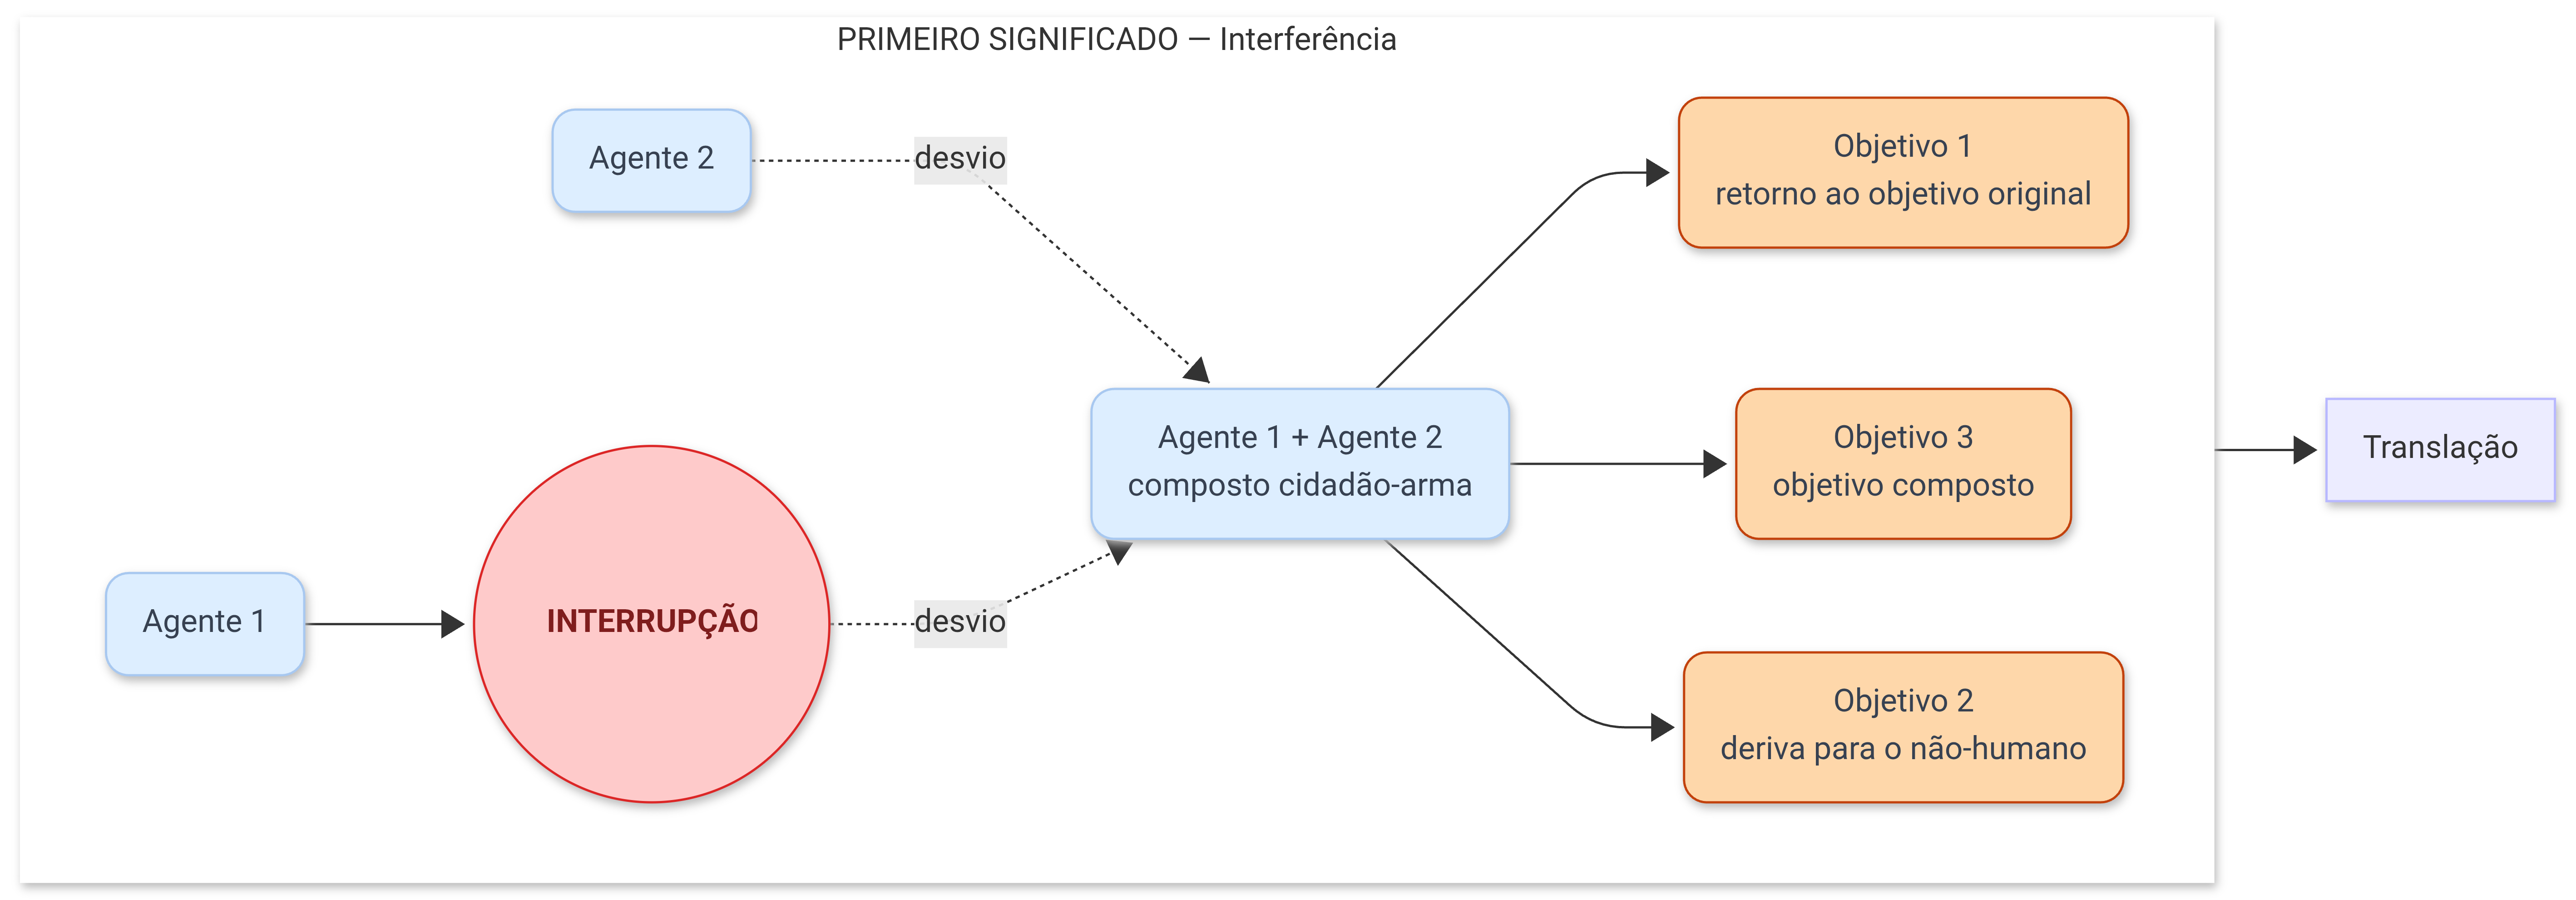
\includegraphics[width=0.6\linewidth]{figuras/cap.2/diagramas/mediacaosignificado_1_traducao.png}
    \caption[Primeiro significado da mediação técnica: tradução de objetivos]{Primeiro significado da mediação técnica, a tradução de objetivos, segundo \textcite{Latour2017Esperanca} (Figura~6.1 do original). O objetivo do Agente~1 é interrompido, o Agente~2 entra por um desvio, e da composição dos dois resulta um terceiro programa de ação, que pode retornar ao objetivo de partida (Objetivo~1), derivar para o objetivo do não humano (Objetivo~2) ou estabilizar-se em um objetivo composto (Objetivo~3). O eixo da translação ordena esses destinos.\url{https://mermaid.ai/d/f1c51456-43c3-424c-8edf-50566fbe40c2}}
    \label{fig:mediacao_significado_1}
\end{figure}

O segundo significado é a composição: a ação é propriedade de uma associação de atores, e não de um agente isolado. Leio aqui o exemplo do voo, que Latour resume na fórmula de que não é o piloto que voa, nem o avião, e sim a associação de aeroportos, pistas, planos de voo, sistemas de navegação, tripulação e companhia aérea. A competência e a ação são propriedades de toda a cadeia de actantes, e por isso a responsabilidade não se imputa a um só deles, e sim se distribui pela associação, no que Latour trata sob o princípio de simetria entre humanos e não humanos: ambos trocam propriedades ao longo das associações que os compõem. Cada agente cujo caminho é interrompido recruta um subprograma por desvio, e os subprogramas se aninham uns nos outros até comporem o objetivo comum, como mostra a Figura~\ref{fig:mediacao_significado_2}.

\begin{figure}[htbp]
    \centering
    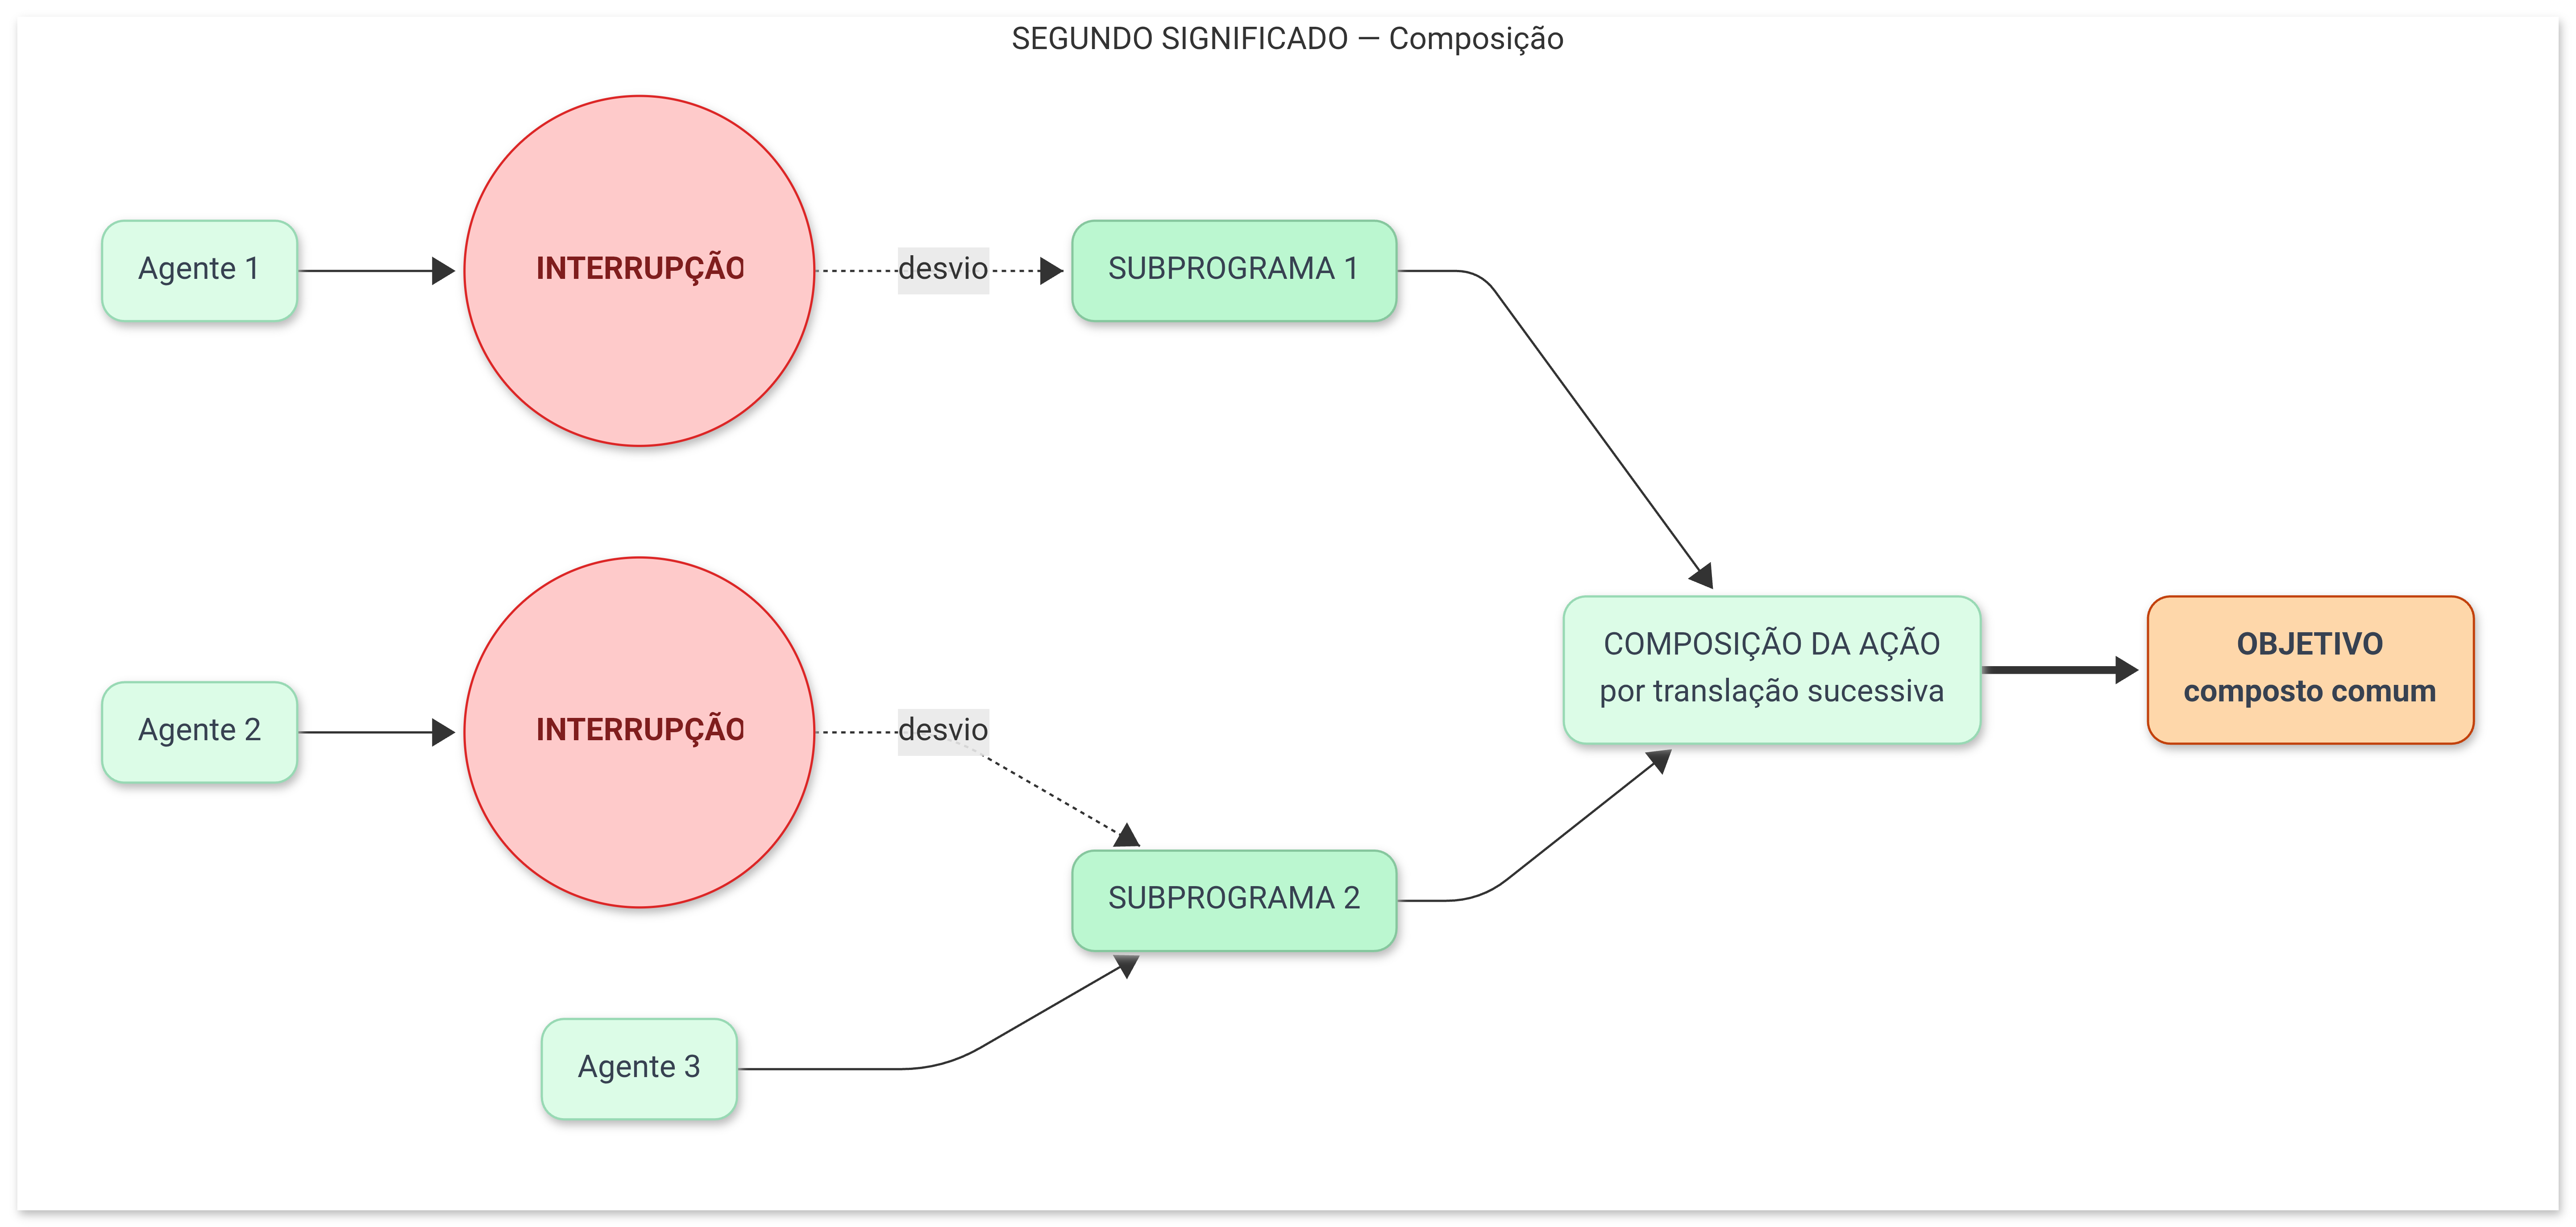
\includegraphics[width=0.6\linewidth]{figuras/cap.2/diagramas/mediacaosignificado_2_composicao.png}
    \caption[Segundo significado da mediação técnica: composição]{Segundo significado da mediação técnica, a composição, segundo \textcite{Latour2017Esperanca} (Figura~6.2 do original). Cada agente que tem o caminho interrompido recruta um subprograma por desvio, e os subprogramas se aninham uns nos outros. A ação é propriedade da associação inteira, e não de um agente isolado, de modo que o objetivo composto comum é alcançado pela composição da ação por translação sucessiva, representada pela linha que se alonga a cada passo acrescentado.\url{https://mermaid.ai/d/050e4650-4240-4681-b65d-825c33579f58}}
    \label{fig:mediacao_significado_2}
\end{figure}

O terceiro significado é o entrelaçamento de tempo e espaço, que Latour também nomeia obscurecimento reversível. Quando uma tecnologia funciona bem, fecha-se como caixa silenciosa, e o número de actantes que a compõem some de vista. Latour toma o retroprojetor que quebra no meio de uma palestra, e em torno do qual reaparecem subitamente as peças, as lâmpadas, os técnicos e os gestos antes invisíveis. O obscurecimento é reversível porque a unidade pode tornar a abrir-se e a fechar-se, e o objeto que contava por um passa a contar por muitos, ou por nenhum. É também aqui que se dá o entrelaçamento do tempo, porque o objeto carrega o trabalho congelado de pessoas distantes e ausentes que continuam a agir através dele no presente, e é por esse mecanismo que a sociedade ganha durabilidade e perdura pela incorporação desses mediadores não humanos, no argumento que Latour condensa no título de \enquote{Technology is Society Made Durable} \parencite{latour1991technology}. A Figura~\ref{fig:mediacao_significado_3} percorre os sete passos desse processo, do desintereste inicial à pontualização da unidade obscurecida.

\begin{figure}[htbp]
    \centering
    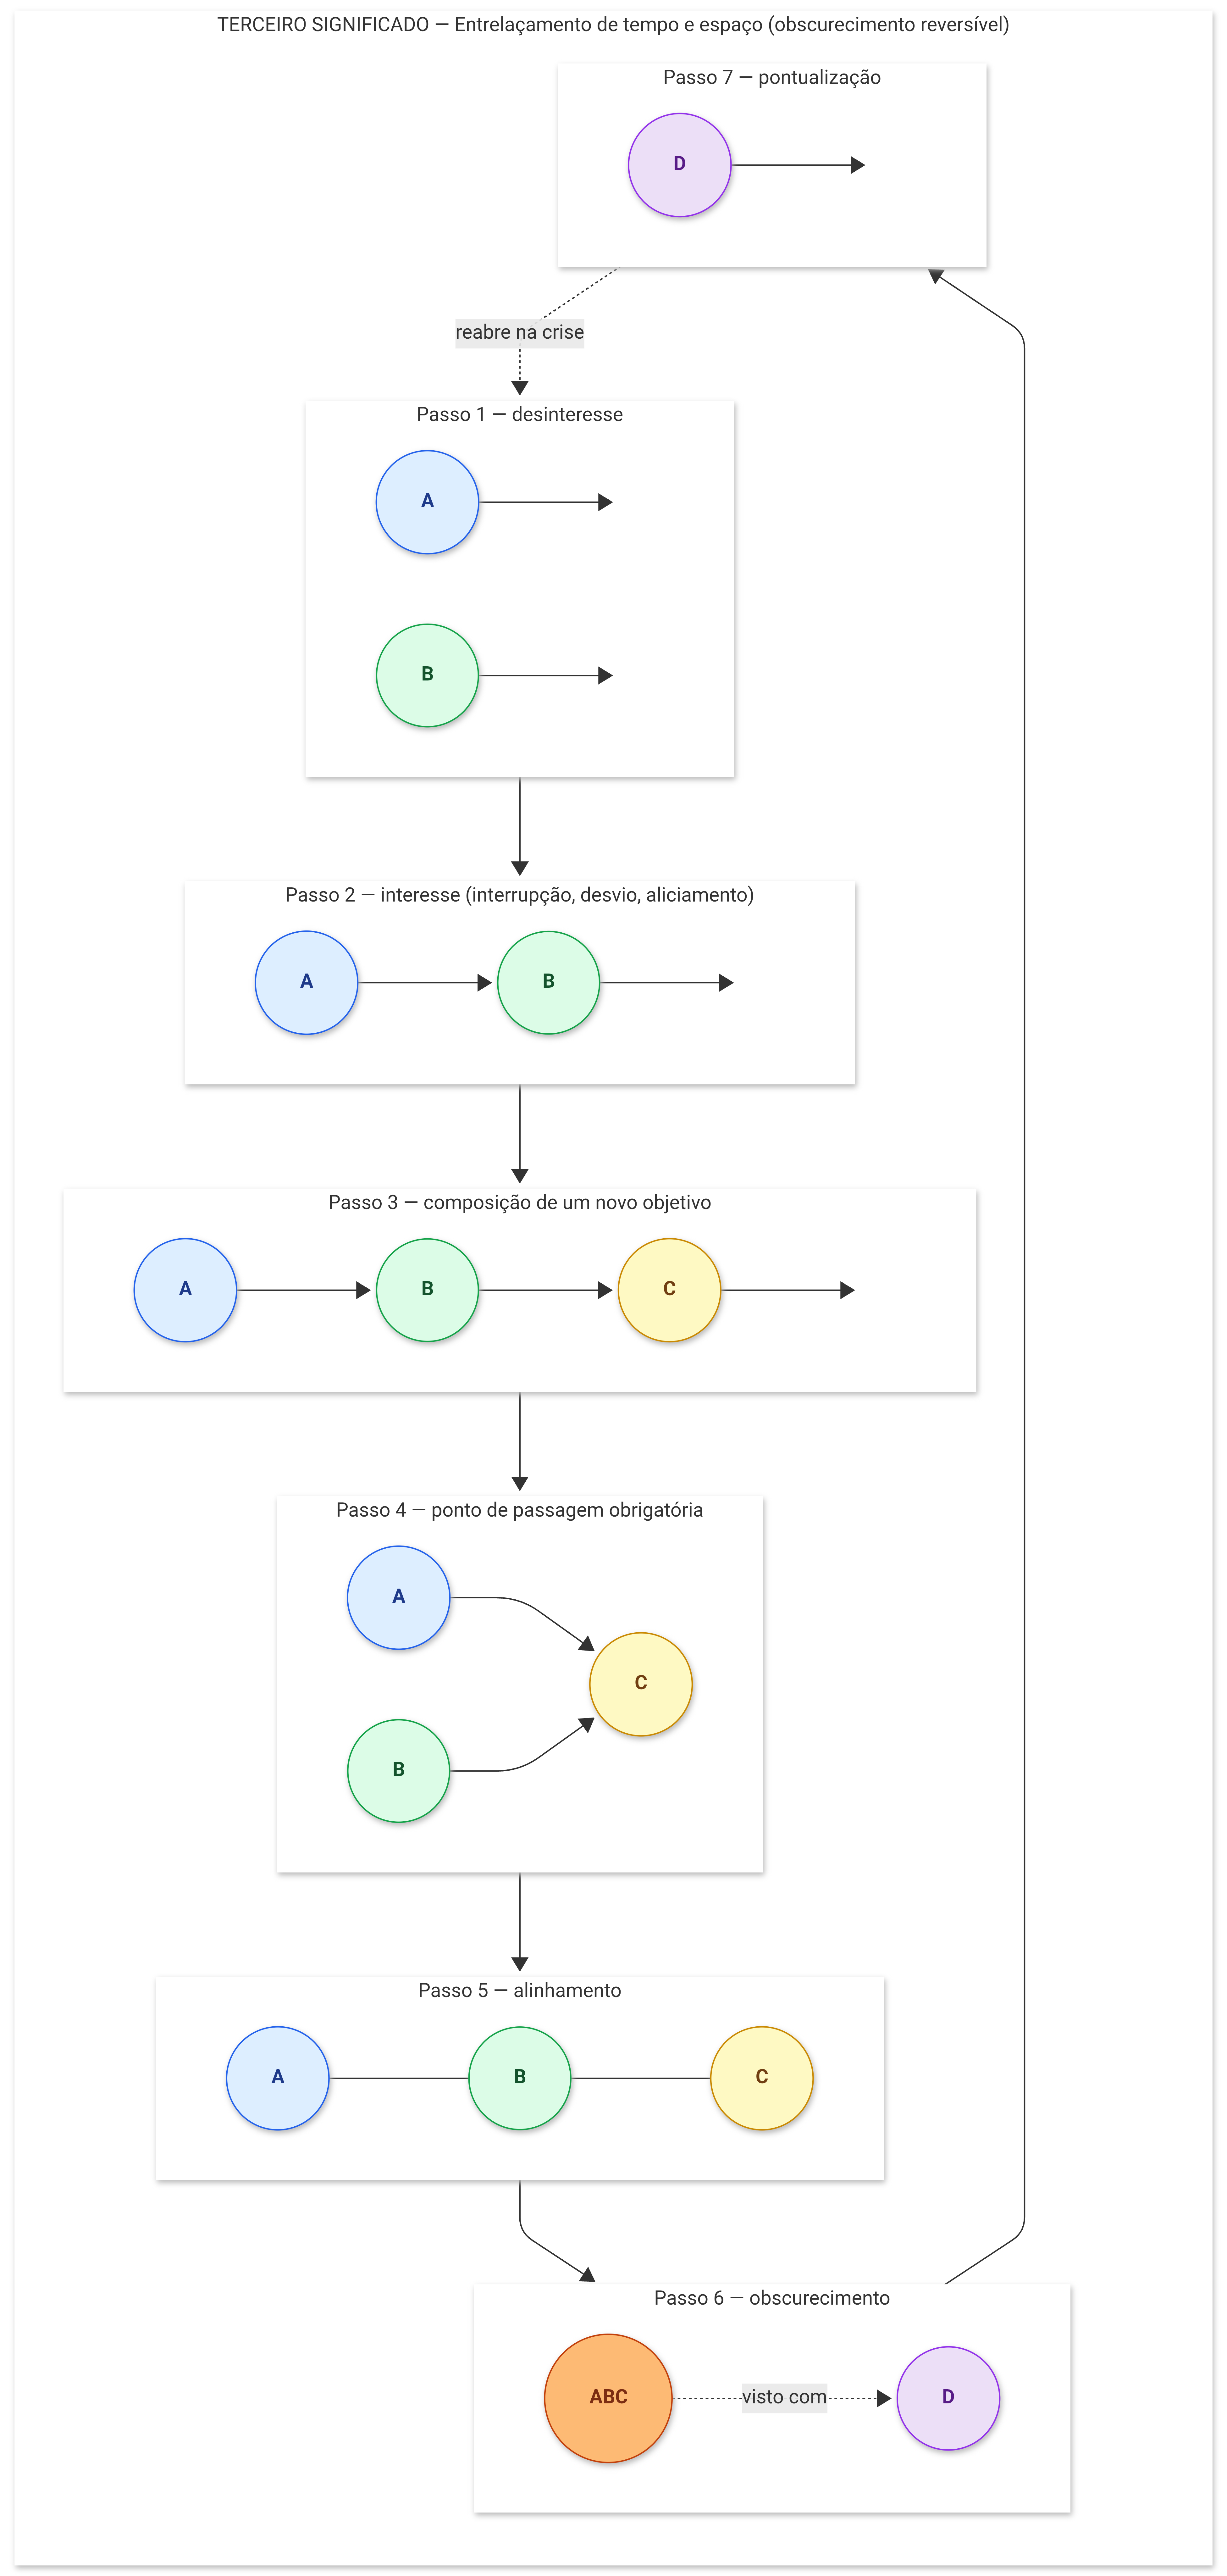
\includegraphics[width=0.5\linewidth]{figuras/cap.2/diagramas/mediacaosignificado_3_obscurecimento.png}
    \caption[Terceiro significado da mediação técnica: entrelaçamento de tempo e espaço]{Terceiro significado da mediação técnica, o entrelaçamento de tempo e espaço, que Latour descreve como obscurecimento reversível, segundo \textcite{Latour2017Esperanca} (Figura~6.3 do original). Os sete passos descrevem como agentes distintos (A, B e C, em cores próprias) deixam de seguir separados (desinteresse), passam a aliciar-se mutuamente (interesse), compõem um novo objetivo, convergem para um ponto de passagem obrigatória, alinham-se, e por fim se obscurecem em uma unidade que circula como um único actante (D, pontualização). As setas de dois sentidos marcam que o processo é reversível, porque a unidade obscurecida pode reabrir-se em uma crise e expor de novo os actantes que a compõem.\url{https://mermaid.ai/d/4b90c964-c828-4b60-ba05-d9b4ee409c69}}
    \label{fig:mediacao_significado_3}
\end{figure}

O quarto significado é a delegação, que Latour descreve como a transposição da fronteira entre signos e coisas: valores, deveres e ordens podem ser inscritos na matéria, de modo que objetos passam a prescrever comportamentos sem vigilância humana contínua. Latour toma o exemplo do quebra-molas (\emph{sleeping policeman}): em lugar de apelar à moralidade dos motoristas com uma placa de \enquote{devagar}, os engenheiros delegam essa ordem ao concreto, e o apelo ético se traduz em obstáculo físico sem deixar de permanecer prescrição, como mostra a Figura~\ref{fig:mediacao_significado_4}.

\begin{figure}[htbp]
    \centering
    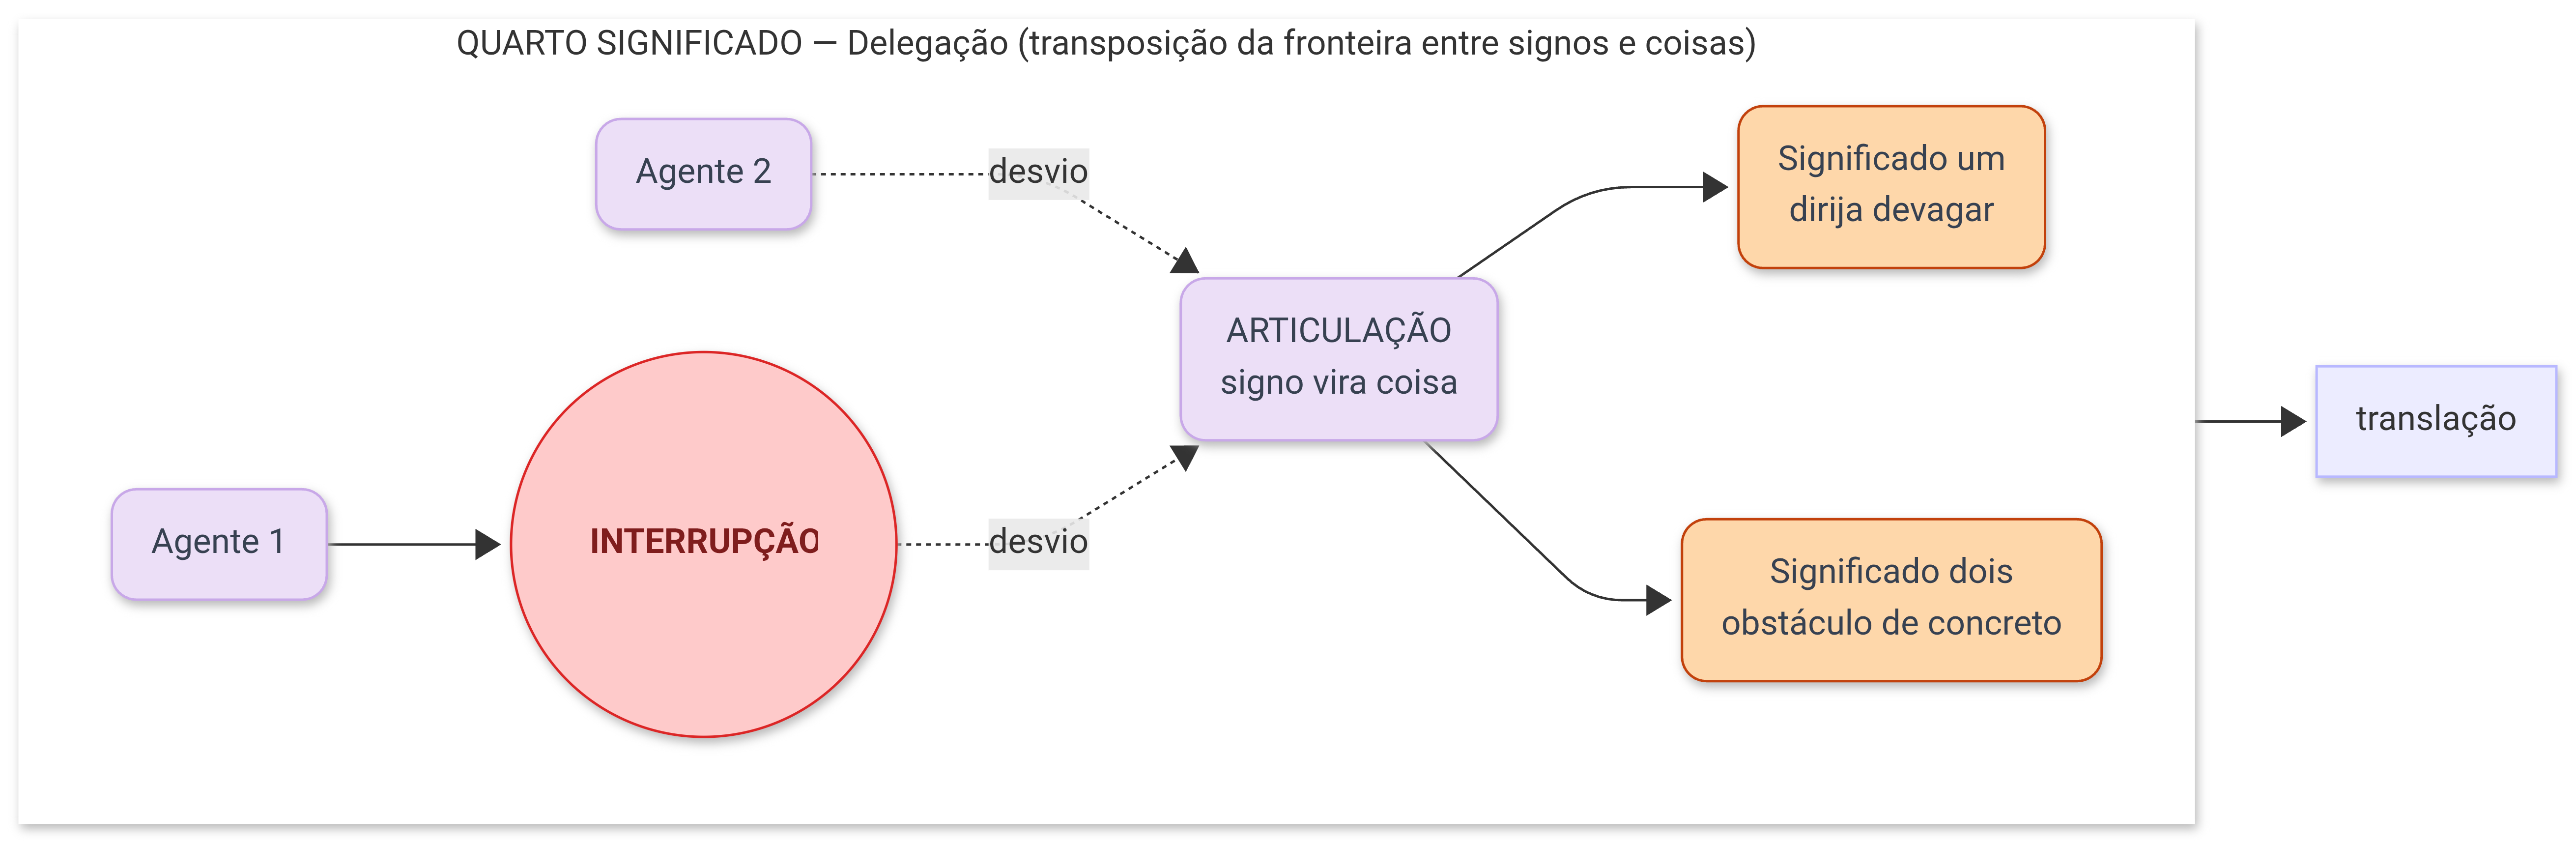
\includegraphics[width=0.6\linewidth]{figuras/cap.2/diagramas/mediacaosignificado_4_delegacao.png}
    \caption[Quarto significado da mediação técnica: delegação]{Quarto significado da mediação técnica, a delegação, que Latour descreve como transposição da fronteira entre signos e coisas, segundo \textcite{Latour2017Esperanca} (Figura~6.4 do original). A estrutura do desvio se repete, agora deslocando não o objetivo, e sim o próprio modo de expressão: um programa de ação humano, a norma \enquote{dirija devagar}, é inscrito na matéria, o quebra-molas, de modo que o Significado um (a prescrição) se traduz no Significado dois (o obstáculo de concreto), e o signo cruza a fronteira que o separa da coisa.\url{https://mermaid.ai/d/fb8411e2-65f0-4a16-a767-fad97bf15f8f}}
    \label{fig:mediacao_significado_4}
\end{figure}

% [NOTA DE REVISÃO 19] Parágrafo que ancora teoricamente a translação e a cadeia de translação, conceito que sustenta os capítulos 3 e 4 e que até aqui era redefinido do zero em cada um deles. Faz aqui, uma vez, a distinção Callon/Latour e a equivalência tradução/translação. As notas dos caps. 3 e 4 remetem a esta passagem. VERIFICAR chave Callon1986Sociology no .bib.
Detenho-me no primeiro significado, a tradução, porque é o que, ao se encadear com outros, sustenta a maior parte da descrição etnográfica que faço nos capítulos~\ref{capitulo3} e~\ref{capitulo4}. \enquote{Tradução} e \enquote{translação} vertem para o português a mesma palavra, \textit{translation} em inglês e \textit{traduction} em francês, e nomeiam o deslocamento pelo qual um actante, ao alistar outro, faz com que objetivos e interesses de partida distintos passem a coincidir, e produz com isso um vínculo que antes não existia e um terceiro programa de ação que nenhum dos actantes possuía sozinho \parencite{Latour2017Esperanca}. Michel Callon e Latour cunham o conceito nos textos fundadores da teoria ator-rede, e os dois o formulam em registros que mantenho distintos ao longo da tese. \textcite{Callon1986Sociology} descreve a translação como percurso de quatro momentos, a \textit{problematização}, o \textit{interessamento}, o \textit{recrutamento} e a \textit{mobilização}, pelos quais um actante se faz porta-voz de outros e desloca os interesses de cada um para um ponto de passagem comum; \textcite{Latour2017Esperanca} a formula como o primeiro dos quatro significados da mediação técnica, o deslocamento de objetivos na troca de propriedades entre humano e não humano. Os dois registros se completam, porque a translação de Callon descreve como os actantes se alistam, ao passo que a tradução de Latour descreve o que acontece com os objetivos de cada um quando o alistamento se dá. Chamo de cadeia de translação a sucessão desses deslocamentos quando um se encadeia ao outro, de modo que o objetivo traduzido por um actante se torna o ponto de partida traduzido pelo seguinte, e a inscrição produzida em uma etapa se torna a matéria-prima da etapa adiante. É essa figura, a do percurso em que cada elo transforma o que recebe do anterior antes de passá-lo ao próximo, que organiza a descrição da trajetória da \texttt{IBM} no capítulo~\ref{capitulo3}, do censo de Hollerith em 1890 à parceria com o \texttt{C4AI}, e a descrição do \texttt{Spira} no capítulo~\ref{capitulo4}, da voz do paciente no \enquote{covideiro} ao argumento científico que circula no artigo. Em ambos, o que sigo é a cadeia inteira de mediação, e por isso assento o conceito aqui, antes de entrar em campo.

% [NOTA DE REVISÃO 1] Parágrafo do radar: corrigida a duplicação "exemplo...exemplo", pontuação diversificada (regra 15).
A passagem do signo para a coisa abre complexidades adicionais quando passo a sistemas tecnológicos como a inteligência artificial. Latour toma o quebra-molas como caso, mas, se penso em um radar eletrônico de velocidade, que tem praticamente o mesmo objetivo, vejo que este alista uma rede muito maior: sensores, câmeras, bancos de dados de placas, sistemas de processamento, notificações automáticas e todo o aparato legal que converte a medição em multa. A mediação técnica deixa de apenas deslocar o apelo ético para o concreto, como no quebra-molas, e passa a multiplicar os actantes e as consequências, e torna a rede mais extensa e mais difícil de mapear à medida que cresce o número de mediações que sustentam uma única ação. Esse aumento de escala, que encadeia muitas traduções em uma só cadeia, é o que me leva dos objetos técnicos de Latour aos sistemas de inteligência artificial.

Os pesquisadores da IA vêm tocando nesse problema por outros caminhos. Durante um seminário transmitido pelo \texttt{C4AI}, no contexto da série \textit{Perspectives in AI}, Cláudio Pinhanez apresentou o problema através da constatação de que a IA generativa produz bons \emph{outputs} para a maioria dos usuários na maior parte do tempo \parencite{Pinhanez2026Seminar}. A fórmula funciona, em sua exposição, como ponto de partida de um deslocamento argumentativo, porque o que ela descreve é a sua intermitência, e não a sua confiabilidade. Em trabalho experimental, \textcite{Pinhanez2025Small} submeteram modelos pequenos, de dois a oito bilhões de parâmetros, a repetições da mesma pergunta, e verificaram que esses modelos com frequência respondem de modos diferentes a cada vez que a pergunta lhes é refeita, ainda que nada na pergunta tenha mudado. A inconsistência é mais aguda justamente nos modelos pequenos, que rodam em infraestrutura modesta e estão mais ao alcance de quem não dispõe de grande capacidade computacional, ao passo que os modelos médios, de cinquenta a oitenta bilhões de parâmetros, e os grandes, na casa dos trilhões, respondem de maneira bem mais estável.\footnote{Pinhanez expõe esses dados na palestra \enquote{The Non-Determinism of LLMs and Other Stability Issues of GenAI}, no seminário \textit{Perspectives in AI} do \texttt{C4AI}, em 29 de abril de 2026, disponível em \url{https://www.youtube.com/watch?v=wiewz65Tg6E} \parencite{Pinhanez2026Seminar}. Na exposição, ele situa o não determinismo como uma de duas instabilidades da IA generativa, ao lado da ausência de limitação local (\textit{local boundedness}), que torna difícil garantir a segurança desses sistemas.} O ponto decisivo é que essa inconsistência é propriedade do próprio mecanismo, e não defeito a corrigir, porque a geração de cada palavra resulta de um sorteio probabilístico, de modo que o mesmo sistema, diante da mesma entrada, pode devolver respostas diferentes a cada passagem. Pinhanez descreve esse traço como uma \enquote{falta de continuidade local, o que torna esses modelos imprevisíveis e incontroláveis}.\footnote{No original: \enquote{GenAI models suffer from lack of local continuity what makes them unpredictable and uncontrollable} \parencite[tradução minha]{Pinhanez2026Seminar}.}

% [NOTA DE REVISÃO 1] Inserida nota que distingue a IA generativa do algoritmo determinístico no sentido corrente, ancorada na primeira menção ao determinismo como princípio da ciência da computação. Trata a confusão comum entre os dois objetos.
Tomo esse fio de \textcite{Pinhanez2026Seminar, Pinhanez2025Small} e o cruzo com o conceito de mediação técnica de \textcite{Latour2017Esperanca} para descrever o que a IA generativa traz de novo. O determinismo era princípio inabalável para a ciência da computação até a IA generativa mostrar que é possível inserir indeterminação e descontinuidade em um sistema computacional, e é esse traço que devolve a discussão à mediação técnica e, ao mesmo tempo, expõe onde ela encontra um objeto que os artefatos de Latour não anteciparam.\footnote{Vale distinguir a IA generativa do algoritmo no sentido corrente, porque os dois são com frequência tomados um pelo outro. Um algoritmo, na acepção clássica da ciência da computação, é uma sequência finita de instruções explícitas que, dada a mesma entrada, produz sempre a mesma saída, e cujo percurso pode ser lido e auditado passo a passo, da ordenação de uma lista ao cálculo de uma rota. É determinístico e inspecionável por construção. A IA generativa não funciona assim. Embora seja executada sobre algoritmos, ela não consiste em regras escritas por um programador, e sim em bilhões de parâmetros ajustados sobre dados de treinamento, dos quais a saída emerge por um sorteio probabilístico a cada termo gerado. Daí as duas propriedades da IA generativa que descrevo nesta seção, o não determinismo e a opacidade, que o algoritmo clássico justamente não tem.}

Sintetizo na figura~\ref{fig:diferencial_ia_mediacao} o que a IA generativa acrescenta à mediação técnica de Latour, e o faço por contraste. O mediador técnico que Latour descreve transforma o que transmite, e nisso a IA generativa não difere de nenhuma outra técnica. A diferença está em outro lugar, e tem três faces que o diagrama dispõe lado a lado. A primeira é que a IA generativa é uma cadeia imensa de mediadores, e não um mediador único: de um lado, os insumos que compõem cada modelo, os dados de treinamento, o trabalho de anotação, o corpus e a curadoria, os parâmetros aprendidos e a infraestrutura de processamento; de outro, os vários modelos de IA que se encadeiam em um sistema em uso, dos quais o modelo generativo é apenas um, ao lado de reconhecedores de fala e visão, modelos de busca e \emph{embedding}\footnote{Um \emph{embedding} é a representação de uma palavra, imagem ou outro dado como um vetor de números, isto é, como um ponto em um espaço de muitas dimensões em que a proximidade entre pontos corresponde a alguma semelhança de sentido ou de uso. O termo vem do aprendizado de máquina, onde nomeia tanto esse modo de representar os dados quanto o modelo que os converte em vetores, e é com base nessa proximidade vetorial que sistemas de busca recuperam itens parecidos com uma consulta. Mantenho o termo em inglês, em vez de traduzi-lo por \enquote{vetor de incorporação} ou \enquote{imersão}, porque é nessa forma que circula entre os pesquisadores com quem convivi em campo.} e classificadores de moderação. A composição que Latour descreve no segundo significado da mediação se multiplica aqui, e cada elo acrescenta a sua própria transformação ao que atravessa a cadeia. A segunda face é o não determinismo. No caso mais controlado que se pode medir, a mesma pergunta feita pelo mesmo usuário e repetida de modo idêntico, a resposta já muda a cada repetição, porque a geração de cada termo resulta de um sorteio probabilístico, e os estudos de \textcite{Pinhanez2025Small} encontram, nos modelos pequenos, consistência em apenas metade a quatro quintos dos casos. Se mesmo nesse caso mínimo a saída varia, a variação só aumenta quando as condições se abrem para usuários, perguntas e formulações distintas, ainda que esse cenário aberto exceda o que o experimento mediu. A terceira face é a não explicabilidade, e o diagrama a formula com cuidado para não sugerir que os engenheiros ignorem o que fazem. Eles conhecem a arquitetura do modelo, os dados com que o treinaram e cada operação que ele executa, e medem o seu comportamento no agregado. O que não conseguem é rastrear, em termos causais legíveis, por que aquela resposta particular saiu daquela vez, porque ao reabrir a caixa não há uma regra escrita a inspecionar, e sim bilhões de parâmetros cuja interação produz a saída sem passar por nenhuma formulação legível. É nesse ponto que a caixa-preta da IA se separa da de Latour. O obscurecimento que descrevi no terceiro significado é reversível justamente porque o que a caixa esconde são mediadores identificáveis um a um, regras e peças que se pode reabrir e conferir, ao passo que a opacidade do modelo persiste mesmo com a caixa aberta. A IA generativa é, então, um mediador no sentido pleno de Latour, e é também um mediador composto por uma multidão de outros mediadores, não determinístico na saída e opaco na decisão, ainda quando tudo o que o constitui é conhecido.

\begin{figure}[htbp]
    \centering
    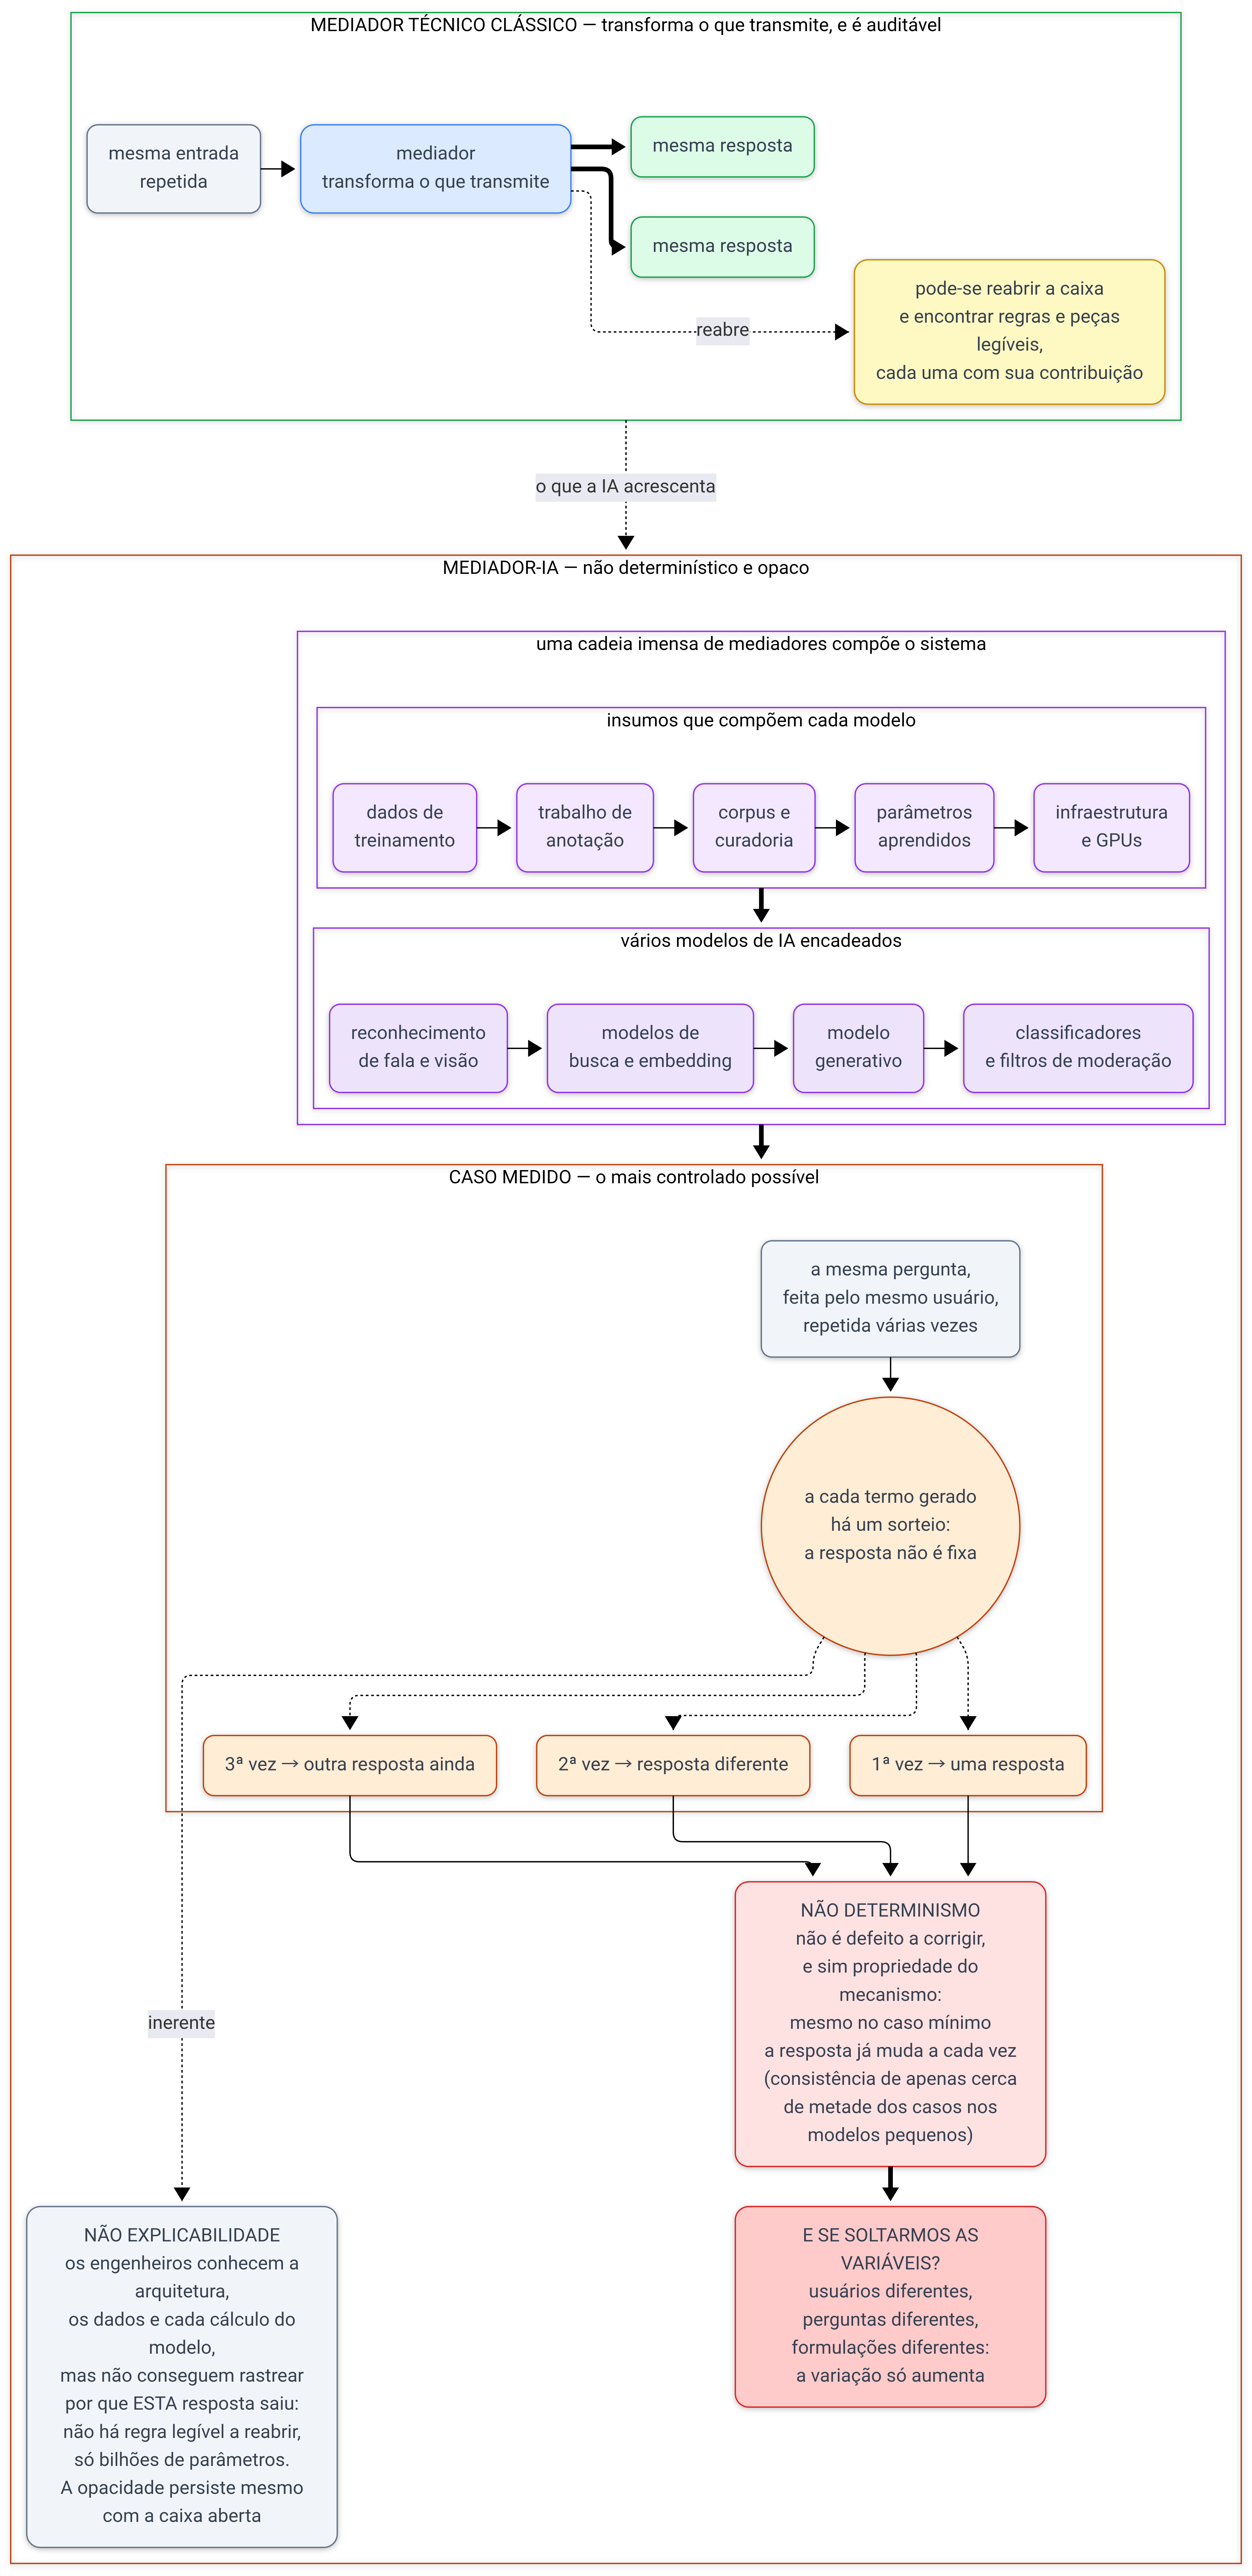
\includegraphics[width=0.5\linewidth]{figuras/cap.2/diagramas/cadeia-mediacao-ia-capitulo2.png}
    \caption[O diferencial da IA generativa na mediação técnica]{O diferencial da IA generativa diante da mediação técnica de Latour. À esquerda, o mediador técnico tal como Latour o descreve: transforma o que transmite, devolve a mesma saída à mesma entrada repetida, e pode ser reaberto e auditado, porque o que a caixa esconde são regras e peças legíveis, cada uma com sua contribuição. À direita, o mediador-IA: o sistema é composto por uma cadeia de mediadores, dos insumos de cada modelo, dados, anotação, corpus, parâmetros e infraestrutura, aos vários modelos de IA encadeados, dos quais o generativo é apenas um. No caso mais controlado que se pode medir, a mesma pergunta feita pelo mesmo usuário e repetida várias vezes, a resposta já muda a cada repetição, porque a geração de cada termo passa por um sorteio probabilístico, e a variação só aumenta quando as condições se abrem para usuários, perguntas e formulações distintas. A caixa permanece opaca mesmo aberta, dado que os engenheiros conhecem a arquitetura, os dados e cada operação do modelo, mas não conseguem rastrear por que aquela resposta particular saiu, já que não há regra legível a reabrir, e sim bilhões de parâmetros.\url{https://mermaid.ai/d/9b29f69e-2c76-465a-b25f-033401bf57c5}}
    \label{fig:diferencial_ia_mediacao}
\end{figure}


A falta de explicabilidade modifica a forma como concebemos a confiabilidade, pois o funcionamento interno do sistema permanece opaco mesmo quando “se abre a caixa” e o que se acessa são apenas inúmeros parâmetros, sem que essa quantidade se converta na regra que efetivamente produziu uma determinada resposta. É isso que permanece não explicável para os desenvolvedores. Tornar o sistema explicável em termos causais vai além do que as arquiteturas atuais permitem; porém, registrar e divulgar o que as medições mostram sobre o comportamento do sistema está, sim, ao alcance de quem o projeta, em que domínios ele tende a alucinar, em que tipos de pergunta a inconsistência é mais frequente, em que cenários a falta de continuidade local se torna mais acentuada. Os dados apresentados por \textcite{Pinhanez2025Small} sobre taxas de inconsistência em função do tamanho do modelo são justamente esse tipo de transparência. Já aos usuários cabe outra tarefa, utilizar os sistemas levando em conta as limitações que os desenvolvedores precisam identificar e explicar. São duas responsabilidades diferentes, e misturá-las produz efeitos importantes, porque, quando a transparência falta do lado de quem constrói, o trabalho de mapear as limitações recai sobre quem usa, não por meio do letramento crítico, mas por tentativa e erro, às custas do usuário e em favor de quem reteve a informação.\footnote{Aproximo essa distinção no capítulo~\ref{capitulo1}, na subseção~\ref{subsec:compostagem3}, em que argumento que a narrativa de \emph{AI literacy} funciona de forma ambígua, ao mesmo tempo em que expressa uma demanda legítima de quem pretende usar IA com autonomia crítica, ela também funciona como deslocamento que transfere ao usuário o encargo de suprir falhas que os desenvolvedores não comunicaram.} Distinguir o que cabe a cada parte é condição para atribuir responsabilidade a quem de fato a detém, em vez de movê-la por completo para o lado do usuário.

O argumento da responsabilidade distribuída tem consequências que excedem o plano da composição individual entre o sistema e o usuário, e que por meio do conceito de mediação técnica é possível aprofundar. Se os desenvolvedores não cumprem a responsabilidade de documentar e comunicar as limitações que conseguem medir, uma das respostas possíveis é a regulação que impeça a circulação de sistemas que não consigam demonstrar a confiabilidade que anunciam.\footnote{O \emph{AI Act} europeu (Regulamento 2024/1689), em vigor desde agosto de 2024, classifica sistemas de IA por nível de risco e impõe requisitos de transparência, documentação e auditoria que variam conforme a classificação. Sistemas de alto risco, incluídos os usados em saúde, educação e emprego, estão sujeitos a avaliação de conformidade antes de chegar ao mercado.} O enquadramento que responsabiliza as empresas que desenvolvem os sistemas é necessário, mas também é insuficiente, porque os erros dessas tecnologias, as alucinações, os vieses de treinamento, a inconsistência que \textcite{Pinhanez2025Small} medem, têm sido tratados como falhas técnicas que melhorias futuras irão corrigir; essa abordagem obscurece que são também parte de um projeto econômico-político que decide o futuro da IA por uma visão de mundo específica: mais dados, mais parâmetros e maior velocidade de lançamento são sempre preferíveis, e os custos dos erros são externalidades que os usuários e a sociedade acabam por absorver \parencite{Brennan2025ArtificialPower}. Essa visão de mundo é produzida e sustentada por uma rede de atores/actantes que inclui empresas de modelos de linguagem, fabricantes de chips e infraestrutura computacional, fundos de investimento que financiam o ritmo de lançamento, pesquisadores que transitam entre academia e indústria, instituições que legitimam os resultados e reguladores que podem favorecer ou beneficiar esse projeto tecnológico. Os debates sobre ética e responsabilidade na IA ganham em precisão quando tomam essa rede como interlocutor, em lugar de cada sistema ou empresa isoladamente. É nesse ponto que a fotografia que abre esta tese, a figura~\ref{fig:dgx1-openai}, com Jensen Huang entregando o DGX-1 a Elon Musk em 2016 enquanto a parede ao fundo anuncia que o destino do mundo depende do uso que se faz do conhecimento, retorna aqui para relacionar o momento em que a infraestrutura que tornaria possível treinar os sistemas que esta seção descreve foi entregue simbolicamente à organização que lançaria o \texttt{ChatGPT} sete anos depois, e o \texttt{C4AI}, herdeiro das possibilidades e dos problemas que essa rede traz consigo, como descrevi no capítulo~\ref{capitulo1}, é um de seus nós brasileiros. Depois de ter percorrido o que a mediação técnica da IA generativa faz e o que ela oculta, fica mais claro por que a tese se inicia com essa imagem e inscreve o problema que os capítulos seguintes perseguem em campo.

A mediação técnica que apresentei há pouco nos seus quatro movimentos aparece na fala de Cláudio de outra forma. Quando ele toma de empréstimo o lema do movimento pelos direitos das pessoas com deficiência, o \textit{nothing about us without us} \parencite{Pinhanez2026Seminar}, e sustenta que a confiabilidade é propriedade de um uso que distribui responsabilidade entre quem constrói, quem regula e quem usa, e não atributo do modelo tomado isoladamente, descreve o que Latour chama de composição, a ação como propriedade de uma associação de actantes. A mediação técnica que trago de Latour e a confiabilidade distribuída que Cláudio mede conectam-se de modo \textit{merográfico}, no sentido que \textcite{strathern2000pse} dá ao termo: formam um par, e cada conceito permanece preso ao seu próprio universo de sentidos, de modo que o que define um não é o que define o outro \parencite[p.~248]{strathern2000pse}.\footnote{O conceito merográfico (do grego \textit{méros}, parte, e \textit{-gráphein}, descrever), que Strathern desenvolve em \textit{Property, Substance and Effect} \parencite{strathern2000pse}, designa uma forma de conexão em que algo se liga a outra coisa por um de seus aspectos, sem que a junção produza uma relação recíproca ou mutuamente definidora. No original, ao analisar o par de Radin entre valores de mercadoria e de não-mercadoria: \enquote{this joining does not yield a reciprocal or mutually defining relation} \parencite[p.~248]{strathern2000pse}. Cada termo do par, escreve Strathern, recorre ao seu próprio universo de conotações, aplicações e sentidos, e é nessa coexistência sem fusão, e não em alguma síntese, que reside o efeito etnográfico da comparação.} Os dois descrevem a agência e a responsabilidade como distribuídas ao longo de uma cadeia de associações entre humanos e não humanos, porém, com efeitos distintos resultantes dessas cadeias. A indeterminação que a análise de \textcite{Pinhanez2025Small} mede, a falta de continuidade local que torna os modelos de IA generativa imprevisíveis, é um problema a resolver, e a confiabilidade distribuída, uma propriedade a garantir. Para a teoria ator-rede, essa mesma indeterminação é constitutiva da translação, que desloca o objetivo a cada translação, dessa maneira, a distribuição da agência não é atributo a aferir, é mais uma cadeia a seguir. É nessa conexão merográfica, em que o mesmo conceito comparece de um lado para nomear um problema a resolver e de outro para descrever uma cadeia a seguir, que está o interesse do cruzamento desses fios.

O cruzamento também faz com que a mediação técnica deixe de ser um conceito que aplico de fora e passa a ser o fio com que sigo, em campo, uma cadeia concreta de translações a partir dos conceitos dos próprios actantes/atores: seja na trajetória da \texttt{IBM} que o capítulo~\ref{capitulo3} segue do censo de Hollerith ao \texttt{C4AI}, e o \texttt{Spira} que o capítulo~\ref{capitulo4} segue desde a voz do paciente às fórmulas e aos gráficos que circulam no artigo científico. O capítulo~\ref{capitulo4} mostra ainda como o conceito de \emph{pipeline}, corrente na ciência da computação, também dialoga com a mediação técnica.\footnote{Um \emph{pipeline}, na ciência da computação, divide um processo em uma série de etapas sequenciais e conectadas, em que a saída de cada etapa é a entrada da seguinte, e é assim que a área identifica e rastreia as associações que faz. A descrição se aproxima da translação latouriana, a cadeia em que cada elo recebe o que o anterior lhe passa e entrega ao próximo, mas os dois conceitos se conectam de modo merográfico: para Latour, a translação desloca o objetivo a cada passagem, e desse deslocamento emerge um terceiro programa de ação que nenhum elo possuía isoladamente, de modo que a transformação é a condição do encadeamento; o \emph{pipeline}, ao contrário, é desenhado para que a saída de uma etapa seja exatamente a entrada que a próxima espera, sem resto e sem desvio, e nele a transformação não prevista conta como erro a corrigir. O capítulo~\ref{capitulo4} acompanha o que acontece quando a translação que a engenharia tenta conter em \emph{pipeline} previsível reintroduz, no \texttt{Spira}, os deslocamentos que o desenho buscava suprimir.} Trazer os conceitos da tecnociência na forma em que os próprios atores os usam mostra que o entendimento dos fenômenos e dos efeitos que esses conceitos nomeiam se faz no cruzamento entre os fios --- os meus e o deles, emaranhados de onde sempre se fazem \enquote{nós}. 

Até aqui acompanhei a mediação da IA generativa observando o que o sistema faz com aquilo que o atravessa e com o que ele oculta: a cadeia de mediadores, o caráter não determinista da saída e a opacidade de como chegou aos resultados que entrega. Agora sigo a mesma cadeia em direção ao que compõe o sistema, porque o conhecimento, os saberes e os dados que o formam não estão fora da mediação. São também mediação que se prolonga para o interior do sistema: cada dado de treino, cada anotação, cada decisão de curadoria é, por si só, uma translação, uma troca de propriedades em que o conhecimento de uma multidão é deslocado, recortado e inscrito no modelo.

A primeira dessas trocas que compõem o sistema é a que nele torna presente o conhecimento coletivo acumulado.\footnote{Matteo Pasquinelli sintetiza a IA como captura da \enquote{inteligência coletiva} que se ergue sobre vastos repositórios de herança cultural e de trabalho coletivo \parencite {Pasquinelli_EyeMaster_2023}. Abordo essa questão com mais detalhes na seção \ref{sec:predicao_poder}.} Esse conhecimento coletivo entra no sistema de IA de forma concreta. Os grandes modelos de linguagem, que funcionam por meio do processamento de linguagem natural e aprendizado de máquina, geram linguagem humana com uma fluência até então inédita, e o fazem porque foram treinados sobre vastos conjuntos de dados que reúnem, em sua maior parte, a produção de inúmeros autores, culturas e contextos, recolhida da internet sob condições de autorização variadas e quase sempre de forma não transparente e por vezes indevida. O que entra no modelo são, assim, camadas de conhecimento, de valor e de expressão tão extensas quanto difíceis de rastrear até as suas origens. Antes, porém, de alimentar o treinamento, esses dados passam por um trabalho que costuma ficar fora de cena, pois alguém precisa organizá-los, classificá-los e rotulá-los, decidir a que tema pertence um texto, se ele é ofensivo, se a resposta a uma pergunta é adequada, ou, quando o dado é uma imagem ou um áudio, o que ali está representado. É sobre os rotuladores que recai essa decisão, e é nas suas mãos que o conhecimento coletivo sofre o primeiro recorte antes de se inscrever no sistema.\footnote{Esse trabalho humano que sustenta sistemas anunciados como automáticos, e que permanece pouco visível na cadeia de produção dos modelos, é o objeto de uma literatura na sociologia do trabalho digital e nos estudos críticos de plataforma, que recomendo como leitura complementar. Mary L.~Gray e Siddharth Suri o nomeiam \emph{ghost work} \parencite{Gray2019GhostWork}, e Kate Crawford o situa na cartografia infraestrutural da IA \parencite{Crawford2021Atlas}. Chamar de \emph{fantasma} esse tipo de trabalho traz à tona a sua condição material precarizada e a sua ocultação que nos sistemas de IA.} Nem todo dado de treino, contudo, vem desse acervo humano e parte é sintética, gerada por um modelo para alimentar outro, de modo que a saída de uma translação anterior reentra na cadeia como matéria-prima da seguinte, e o sistema passa a aprender, em alguma medida, sobre o que ele próprio já produziu.\footnote{Quando os dados sintéticos predominam no treinamento, descreve-se o risco do chamado colapso de modelo (\emph{model collapse}): ao aprender cada vez mais sobre as próprias saídas, e cada vez menos sobre o acervo humano de origem, o modelo tende a estreitar a variedade do que gera e a amplificar os seus próprios desvios, geração após geração. Esse problema torna ainda mais evidente a dependência que a cadeia tem do material humano que lhe dá origem.}

Dessa maneira, os sistemas de IA colocam um novo desafio para a teoria ator-rede: descrever uma rede sociotécnica exigiria seguir os mais variados elementos e as agências que neles se distribuem, tarefa cuja vastidão as genealogias e as cartografias de sistemas de IA de Kate Crawford e Vladan Joler fazem perceber serem gigantescas e opacas \parencite{Crawford2018Anatomy}. Uma vez que é impossível seguir essas redes por inteiro, e que nenhuma descrição daria conta dessa tarefa, mesmo em redes bem menos extensas, como discuti no capítulo~\ref{capitulo1}, na seção~\ref{subsec:cortando-redes}, o que os dois fios desta seção me deixam fazer é outra coisa, mais modesta, e suficiente. Com o conceito de mediação técnica sigo as cadeias de translação, a distribuição de propriedades e de responsabilidades, em momentos e sítios etnográficos específicos, a partir de actantes e de sistemas de IA particulares.

O que torna essas cadeias rastreáveis, porém, são as coisas que ficaram para trás, os rastros, os vestígios que foram apagados, ocultados, suprimidos ou transformados na construção dos sistemas tecnocientíficos --- entre essas coisas, \textit{pessoas}. No capítulo~\ref{capitulo4}, refaço a cadeia de translação a partir do conceito de \textit{inscrição}, no sentido que \textcite{Latour1986Visualization, Latour2011CienciaEmAcao, Latour1986Writing} dão ao termo --- e que chamo de \textit{inscrições tecnocientíficas} ---, as representações portáteis e combináveis, gráficos, tabelas, fórmulas, coeficientes, artigos, em que o trabalho tecnocientífico fixa e faz circular.\footnote{Em \textit{Visualisation and Cognition: Drawing Things Together}, \textcite{Latour1986Visualization} descreve o trabalho científico não como ação direta sobre o mundo, mas sobre inscrições, representações bidimensionais que transformam fenômenos em traçados que podem ser lidos, combinados, transportados e acumulados. A força dessas representações vem de uma propriedade que Latour nomeia móveis imutáveis (\emph{immutable mobiles}): elas se deslocam e se sobrepõem sem se deformar. Desenvolvo o conceito no capítulo~\ref{capitulo4}, onde acompanho a cadeia de inscrições do \texttt{Spira}, da voz do paciente ao espectrograma e ao argumento que circula no artigo científico.} É por essas inscrições que investigo, no capítulo~\ref{capitulo4}, o modo como o \texttt{Spira} é feito e como se fixa e circula na tecnociência. No capítulo \ref{capitulo4}, diferente do capítulo \ref{capitulo3}, o que sigo são os traçados já estabilizados de um sistema de IA, e a posição de onde os acompanhei eu já a situei no capítulo \ref{capitulo1}, na seção \ref{onde-esta-laboratorio-cientistas}. São esses traçados que, lidos a contrapelo, deixam entrever o processo que procuravam fechar, e devolvem à análise as pessoas e as coisas que havia deixado para trás.

Seguir essas cadeias por inteiro é impossível, e nenhuma descrição daria conta da tarefa, mesmo em redes bem menos extensas, como discuti no capítulo~\ref{capitulo1}, na seção~\ref{subsec:cortando-redes}. As genealogias e as cartografias de sistemas de IA de Kate Crawford e Vladan Joler fazem perceber o quanto essas redes são vastas e opacas \parencite{Crawford2018Anatomy}, e essa vastidão não é só uma dificuldade de método. A extensão da rede, o número de actantes que ela alista e a opacidade que a atravessa são também efeitos de poder, porque é ao longo dessas cadeias que se distribuem de forma desigual os recursos, a infraestrutura e a autoridade que sustentam os sistemas de IA.

Os temas que mapeei na seção~\ref{sec:estudos_ciencia_tecnologia} recompõem as tradições fundadoras dos estudos de ciência e tecnologia e seus desdobramentos para o digital, que, de diferentes maneiras, orientam esta tese. Além disso, os precedentes de Forsythe e Collins reunidos nessa seção posicionam minha pesquisa em uma linhagem antropológica, etnográfica e sociológica que já vem se dedicando à inteligência artificial desde os anos 1980. A seção seguinte retoma justamente o ponto em que a rede tecnocientífica se torna tão extensa e opaca que se torna necessário investigar por que ela assume essa configuração antes de partir para suas ramificações localizadas e situados como o \texttt{C4AI}. Os estudos de engenharia e as culturas de predição em Johnson e Lenhard permitem acompanhar a coevolução entre as práticas de previsão e as infraestruturas computacionais ao longo de século para entender como chegamos a isso, enquanto as genealogias críticas do poder tecnológico em Pasquinelli, Crawford e Joler trazem elementos para pensar a conjuntura global e histórica da economia extrativista que sustenta os sistemas de inteligência artificial, para os quais, a opacidade é uma questão fundamentalmente sociotécnica, ou seja, de poder e capital.

\section{Tecnociência e poder: ficções do Antropoceno}
\label{sec:predicao_poder}

\epigrafe{%
Isso se torna uma estrutura complexa de cadeias de fornecimento dentro de cadeias de fornecimento, um zoom fractal de dezenas de milhares de fornecedores, milhões de quilômetros de transporte de materiais e centenas de milhares de trabalhadores incluídos no processo mesmo antes de o produto ser montado na linha.}%
{Kate Crawford e Vladan Joler, \textit{Anatomia de um sistema de inteligência artificial}, trad. Cristiana Gonzalez e Pedro P. Ferreira, 2020.}

Quando os geólogos propuseram nomear de Antropoceno a época em que a ação humana passou a agir na mesma escala dos rios, dos vulcões e da composição química da atmosfera, trouxeram à tona uma figura que as ciências humanas julgavam ultrapassada, a do \textit{Anthropos} \parencite[p.~117]{Latour2017FacingGaia}. O problema é que esse \textit{Anthropos} não existe como ator único. Latour observa que não há como unificar o humano em um agente dotado de consistência moral ou política a ponto de responsabilizá-lo pela escala geológica de suas ações, e que falar de uma \enquote{origem antrópica} do aquecimento global perde o sentido se por antrópico se entende a espécie humana em geral, porque ninguém pode pretender falar pelo humano em geral sem provocar mil protestos \parencite[pp.~120--121]{Latour2017FacingGaia}.\footnote{No original: \enquote{there is no way to unify the Anthropos as an actor endowed with some sort of moral or political consistency} \parencite[p.~121, tradução minha]{Latour2017FacingGaia}. O argumento se desdobra em \textit{Down to Earth} \parencite{Latour2018DownToEarth}, onde Latour liga a recusa do \textit{Anthropos} genérico à distribuição radicalmente desigual das responsabilidades e dos custos entre as elites que se beneficiam da extração e a maioria que arca com ela.} A espécie humana genérica é uma ficção, e uma ficção que apaga quem decide, quem lucra e quem paga.

Para Haraway, as respostas aos horrores dessa época vêm derivando de uma fé cômica, a \emph{technofix}, de que a tecnologia, de algum modo, salvará os humanos de suas mazelas \parencite[p.~3]{Haraway2016Staying}.\footnote{No original: \enquote{a comic faith in technofixes, whether secular or religious: technology will somehow come to the rescue of its naughty but very clever children} \parencite[p.~3, tradução minha]{Haraway2016Staying}. Haraway aproxima a salvação pela máquina da salvação divina, \enquote{or what amounts to the same thing, God will come to the rescue}, lendo a \emph{technofix} como uma narrativa de redenção que projeta o conserto sobre um salvador externo. Ela recusa essa fé sem, no entanto, recusar a técnica: na mesma página, sustenta que \enquote{it remains important to embrace situated technical projects and their people. They are not the enemy} \parencite[p.~3, tradução minha]{Haraway2016Staying}. À \emph{technofix} ela não opõe a recusa da tecnologia, e sim o gesto de \enquote{staying with the trouble}, permanecer no problema junto a projetos técnicos situados e às pessoas que os fazem, em vez de fugir para a promessa da máquina ou para o desespero do \enquote{game over}, atitude que ela considera ainda mais destrutiva que a primeira.} O \emph{technofix} é a forma tecnocientífica da mesma ficção: assim como o \textit{Anthropos} postula um sujeito único que teria causado a crise, a fé na correção técnica postula um saber único, soberano e separado do mundo que ele manipula, capaz de resolvê-la de fora, sem que ninguém em particular precise mudar de posição, abrir mão de um lucro ou responder por danos. As duas figuras produzem um agente abstrato, a espécie, a Técnica, precisamente para deixar na sombra os actantes situados que decidem, se beneficiam e arcam com as consequências. A recusa de Haraway ao \emph{technofix} não é, portanto, uma recusa da técnica, e sim uma recusa de uma figuração que abstrai a técnica de seus projetos situados e de suas pessoas, e é nessa brecha, entre a Técnica que salva de fora e os projetos técnicos que se fazem por dentro do problema, que esta tese parte. A promessa de que a inteligência artificial resolverá problemas que ela própria ajuda a agravar, da extração de recursos naturais ao consumo energético dos seus \emph{datacenters} à concentração de poder de quem a controla, é uma versão desse \emph{technofix} que anuncia a salvação pela máquina e, no mesmo gesto, apaga as cadeias materiais e econômicas que fazem essas tecnologias possíveis e que distribuem desigualmente os seus custos e seus benefícios.

É nesse ponto que a inteligência artificial entra nesta seção, como o caso em que a ficção do humano genérico e a promessa da salvação técnica se encontram em sua forma mais atual. A inteligência artificial é apresentada, com frequência, como conquista da humanidade, um \textit{nós} que avança no conhecimento. Os relatórios anuais do AI Now Institute mostram o trabalho que essa narrativa realiza: tratar a IA como sinônimo de progresso e como trajetória inevitável é o que impede o controle público sobre o rumo desses sistemas, e nada na inteligência artificial tem de inevitável \parencite[p.~5]{Kak2023Confronting}.\footnote{No original: \enquote{there is nothing about artificial intelligence that is inevitable. Only once we stop seeing AI as synonymous with progress can we establish popular control over the trajectory of these technologies} \parencite[p.~5, tradução minha]{Kak2023Confronting}. No relatório de 2025, o mesmo movimento reaparece sob a mitologia da \enquote{inteligência artificial geral}, cujo efeito é colapsar a complexidade técnica em um futuro único e iminente que \enquote{conveniently advances the interests of the companies claiming to build it} \parencite[p.~10, tradução minha]{Brennan2025ArtificialPower}.} Essa figura do \textit{nós} que avança apaga a desigualdade com que se distribuem os custos materiais desses sistemas, a energia, a água, os minerais, o trabalho de anotação precarizado, e os seus benefícios, a concentração de capital e de capacidade computacional. O relatório recupera o argumento de \textcite{Bender2021Stochastic}, segundo o qual pessoas marginalizadas e do Sul Global são as mais expostas aos danos ambientais do consumo energético e das emissões dos grandes modelos de linguagem, ao mesmo tempo em que são as menos prováveis de colher seus benefícios, dado que apenas uma pequena elite global tem condições de desenvolvê-los \parencite[p.~33]{Kak2023Confronting}. Descrever essa desigualdade exige sair da figura do humano e da tecnologia genéricos e seguir a rede concreta de actantes que produz e sustenta esses sistemas.

Um exemplo de como seguir essa rede são os trabalhos cartográficos que Kate Crawford e Vladan Joler montaram a partir do assistente \texttt{Amazon Echo}, que seguiram uma cadeia de actantes que um único comando de voz convoca \parencite{Crawford2018Anatomy}. Quando alguém pede a um cilindro de plástico na sala de estar que acenda a luz, entra em ação uma cadeia que vai do lítio do Salar de Uyuni, na Bolívia, às minas de cobalto do Congo, dos contêineres padronizados que atravessam o sistema vascular da fábrica global aos \emph{datacenters} que processam a voz, e dos trabalhadores que montam o aparelho na linha da Foxconn aos que, no outro extremo, classificam dados de treinamento por frações de centavo. Crawford e Joler nomeiam o usuário desse arranjo como figura híbrida, consumidor, recurso, trabalhador e produto ao mesmo tempo, porque cada interação devolve ao sistema os dados que o aperfeiçoam. O que essa cartografia torna descritível é a desproporção entre o gesto e a rede que o sustenta, uma vez que a escala dos recursos exigidos para acender uma luz por comando de voz excede em muitas ordens de grandeza a energia e o trabalho que a mesma ação pediria a um interruptor de parede, e a contabilidade completa desse custo permanece, segundo os autores, quase impossível de fechar. Em \textit{Calculating Empires}, Crawford e Joler estendem o gesto cartográfico para cinco séculos, e tratam comunicação, computação, classificação e controle como dimensões de um mesmo regime de poder que recua à expansão imperial europeia a partir de 1500, com o intuito de mostrar como os padrões tecnológicos de colonialismo, militarização, automação e cercamento ainda subjugam e como poderiam ser desfeitos \parencite{Crawford_Joler_CalculatingEmpires_2023}.\footnote{Reúno aqui os endereços das cartografias citadas. \textit{Anatomy of an AI System} \parencite{Crawford2018Anatomy} segue a cadeia material do \texttt{Amazon Echo}, do minério ao lixo eletrônico, e está disponível em: \url{https://anatomyof.ai}; há tradução brasileira de Cristiana Gonzalez e Pedro P. Ferreira, com colaboração de Pedro Paulino, publicada na revista \textit{ComCiência} em 2020, em: \url{https://www.comciencia.br/anatomia-de-um-sistema-de-inteligencia-artificial/}. \textit{Calculating Empires: A Genealogy of Technology and Power Since 1500} é visualização de pesquisa em larga escala que rastreia a coevolução das estruturas técnicas e sociais ao longo de cinco séculos, organizada em torno dos quatro eixos de comunicação, computação, classificação e controle, e está disponível em: \url{https://calculatingempires.net}. Os dois integram, com o \emph{Nooscópio} \parencite{pasquinelli2020nooscope}, disponível em \url{https://nooscope.ai} e em tradução brasileira de Leandro Módolo e Thais Pimentel publicada pela \texttt{LAVITS} em 2020, em: \url{https://lavits.org/o-manifesto-nooscopio-inteligencia-artificial-como-instrumento-de-extrativismo-do-conhecimento/}, uma série de cartografias críticas da inteligência artificial que Vladan Joler vem montando em coautoria, ora com Kate Crawford, ora com Matteo Pasquinelli. A essa série pertence também o \textit{New Extractivism}, que Joler assina sozinho e descreve como uma \emph{assemblage} de conceitos e alegorias, um mapa alegórico do extrativismo digital que reúne figuras como o buraco negro das plataformas, a alegoria da caverna e o triângulo do trabalho digital, e que o próprio autor declara construído a partir do \textit{Anatomy} e do \emph{Nooscópio} \parencite{Joler_NewExtractivism_2020}, disponível em: \url{https://extractivism.online}. Em registro próximo, o coletivo Estampa adotou estrutura cartográfica análoga para descrever a inteligência artificial como sistema extrativista e estruturalmente dependente em escala global \parencite{Estampa_Cartografia_IA}, em mapa disponível em: \url{http://cartography-of-generative-ai.net}. Acesso a todas em: 6 abr.~2026.} O capítulo~\ref{capitulo3} percorre uma rede análoga de forma situada, da máquina de tabulação que Herman Hollerith desenvolveu para o censo americano de 1890 ao convênio \texttt{C4AI}-\texttt{IBM} assinado em 2020. Onde Crawford e Joler cartografam essa rede pela via histórica, eu a percorro etnograficamente, e me inspiro neles para descrever o que ela articula, a classificação, o controle e a infraestrutura computacional, e o modo como, ao se desdobrar fora dos Estados Unidos e chegar até o Brasil, atualiza relações de dependência tecnológica e infraestrutural.

A essa rede material da inteligência artificial se liga outra rede de extração, que Matteo Pasquinelli e Vladan Joler desenvolvem a partir da figura do \emph{Nooscópio}, um diagrama que mapeia a cadeia de associações pela qual o conhecimento é extraído e convertido em um modelo estatístico que devolve como cálculo automático da máquina o trabalho social do qual foi destilado \parencite{pasquinelli2020nooscope}. Esse diagrama pode ser lido junto com o \textit{Anatomy of an AI System} \parencite{Crawford2018Anatomy}, que acompanha a matéria, do minério ao lixo eletrônico, enquanto o \emph{Nooscópio} acompanha a informação, do dado de treinamento ao modelo estatístico. A leitura cruzada dos dois mapas permite entender a inteligência artificial como o ponto de interseção entre uma cadeia de extração de matéria e uma cadeia de extração de conhecimento. Pasquinelli e Joler explicam o aprendizado de máquina em analogia ao instrumento óptico, um nooscópio que amplia a visão do conhecimento, e mostram, a partir daí, que a matéria-prima desse instrumento vem do trabalho social acumulado, ou seja, as imagens, os textos e os sons que pessoas produziram e que são capturados, rotulados e comprimidos em um modelo estatístico. A parábola do \texttt{ImageNet}\footnote{O \texttt{ImageNet} é um conjunto de dados de imagens construído entre 2007 e 2009 por uma equipe coordenada por Fei-Fei Li em Princeton e Stanford, publicado em 2009 e organizado em cerca de catorze milhões de imagens distribuídas segundo a taxonomia lexical do \texttt{WordNet}. Tornou-se a infraestrutura de referência da visão computacional sobretudo a partir do desafio anual de reconhecimento que sediou de 2010 a 2017, o \texttt{ImageNet Large Scale Visual Recognition Challenge}; foi nele, em 2012, que a rede neural convolucional \texttt{AlexNet} reduziu drasticamente a taxa de erro de classificação e marcou a virada do campo para o aprendizado profundo. Reconstruo a história do conjunto e os seus efeitos a partir de \textcite{Luccioni2024NineLives}, que o examina como infraestrutura sociotécnica e questiona o essencialismo embutido em suas categorias automáticas; sobre a camada de rotulagem e a herança problemática das categorias do \texttt{WordNet}, em especial as ofensivas e as que atribuem identidades a partir da aparência, ver \textcite{Crawford2019ExcavatingAI}.} condensa o argumento, pois o conjunto de dados que deu partida ao aprendizado profundo em 2012 foi montado com imagens baixadas de serviços abertos, depois organizadas pela taxonomia do \texttt{WordNet} e rotuladas por trabalhadores anônimos do Sul Global que recebiam centavos por tarefa na plataforma \texttt{Amazon Mechanical Turk} da \texttt{Amazon}. Em ambos os mapas, portanto, o trabalho que faz a inteligência artificial parecer autônoma permanece escondido atrás da interface, e é aqui que a desigualdade que anunciei acima ganha a sua forma concreta, já que os \emph{pipelines}\footnote{O termo \emph{pipeline} designa, na engenharia de software e no aprendizado de máquina, a sequência encadeada de etapas pelas quais os dados passam, da coleta bruta ao modelo treinado, em que a saída de cada etapa é a entrada da seguinte. Importo o termo da comunidade de prática da ciência de dados, e o mantenho em itálico para preservar a estranheza de uma palavra que naturaliza, na imagem do nooscópio, o trabalho humano disperso que Pasquinelli e Joler trazem à tona \parencite{pasquinelli2020nooscope}.} de tarefas vão do Norte Global para o Sul Global, ao passo que os territórios de dados são dominados por poucas companhias que controlam tanto a infraestrutura quanto os modelos dela extraídos.

Se as cartografias de Crawford, Pasquinelli e Joler descrevem as cadeias de extração que sustentam a inteligência artificial no presente, o trabalho de Ann Johnson e Johannes Lenhard me dá o fio histórico que falta a esses mapas, o de como se chegou às práticas de predição que a inteligência artificial leva ao limite. Esse fio dialoga com esta tese em particular no capítulo~\ref{capitulo3}, no qual analiso o papel histórico da \texttt{IBM} na criação e organização de ecossistemas de inovação em IA. Em \textit{Cultures of Prediction: How Engineering and Science Evolve with Mathematical Tools} \parencite{JohnsonLenhard2024}, Johnson e Lenhard apresentam a previsão científica e de engenharia como práticas historicamente dinâmicas, e tensionam a percepção que toma a previsão por ferramentas matemáticas como bloco monolítico estático no tempo. Ao estudar práticas de previsão ao longo de quatro séculos, os autores sustentam que a matematização das coisas e do mundo é um conceito flexível, e que os métodos de previsão, as concepções de matematização e a tecnologia coevoluíram. O conceito central que os autores elaboram, \textit{cultura da predição} (\textit{culture of prediction}), nomeia precisamente essa coevolução: o termo \textit{cultura} salienta que modos de previsão, matematização, epistemologia, tecnologia e organização social se desenvolvem juntos e se estabilizam um em relação ao outro. Não se trata de uma época, mas de um tipo ideal, no sentido weberiano, que nunca se realiza em estado puro em momento algum, e que funciona como orientação para a prática de quem prevê; é por isso que as culturas se sobrepõem em vez de se sucederem, pois modos e culturas mais antigos persistem enquanto novos se desenvolvem ao lado deles. O conceito traz consigo, ainda, um deslocamento na filosofia da ciência, ao tratar teorias e modelos menos como dispositivos que explicam e mais como dispositivos que preveem. Os autores identificam quatro dessas culturas: a \textit{racional}, nascida nos séculos XVI e XVII, em que a matemática captura a estrutura dos fenômenos e a previsão se deriva de leis gerais; a \textit{empírica}, que abre mão dessa generalidade em favor da flexibilidade com que um modelo se ajusta à observação; a \textit{iterativa-numérica}, que emerge com as tecnologias de cálculo do século XIX e se estabiliza com as máquinas \textit{mainframe}, ao pôr a repetição sucessiva de algoritmos simples no centro da matematização; e a \textit{exploratória-iterativa}, que surge com os computadores pessoais em rede por volta de 1990, quando o trabalho sobre modelos passa a investigar relações entre dados de entrada e de saída em troca rápida entre modelos e modeladores. O que retenho desse percurso para esta seção é que prever, nessa história, nunca esteve longe de controlar, pois controlar um sistema supõe antecipar como ele se comportará, e é essa proximidade entre predição e controle que faz das culturas da predição não apenas um capítulo da história da matematização, mas um fio da mesma genealogia de poder que as cartografias da extração explicitam.

Dessas quatro culturas, é a última que mais me interessa, porque é nela que a inteligência artificial contemporânea se inscreve e é dela que Johnson e Lenhard projetam o passo seguinte. Na cultura exploratória-iterativa, o valor dos modelos preditivos cresce nas abordagens baseadas em computador, da simulação ao aprendizado de máquina, e o modo de produção de conhecimento que ela instala é o que os autores chamam de \textit{design} (\textit{design mode of knowledge production}), isto é, um modo que se concentra menos em explicar um fenômeno e mais em construir artefatos e testar o seu desempenho preditivo. É o ponto em que o deslocamento que apontei acima, das teorias que explicam para os modelos que preveem, ganha sua forma técnica mais acabada, e é também o ponto a partir do qual os autores arriscam a hipótese de uma quinta cultura: a investigação do que denominam \enquote{previsão pura} (\textit{pure prediction}), em emergência a partir do aprendizado profundo e das redes neurais. O que torna essa previsão \enquote{pura}, para Johnson e Lenhard, é que ela classifica correlações entre conjuntos enormes de dados por meio do ajuste automático de milhões de parâmetros que nenhum humano consegue percorrer, de modo que o modelo prevê bem sem que reste algo a explicar. Dessa maneira, a pergunta sobre por que o sistema previu isto e não aquilo perde o objeto, e o critério clássico de uma boa teoria, o de representar adequadamente aquilo que estuda, perde-se por completo.\footnote{Johnson e Lenhard ilustram a previsão pura com o primeiro acidente fatal de um automóvel em piloto automático, um Tesla que, em 2016, tomou um trailer branco por uma placa de trânsito suspensa e não freou; à pergunta sobre por que a rede neural fez uma previsão tragicamente errada, os autores respondem que não há resposta no sentido causal, pois \enquote{por que exatamente} o trailer era, para a rede, semelhante a uma placa escapa à explicação humana, sendo apenas o que a rede aprendeu à maneira dela \parencite[pp.~197--199]{JohnsonLenhard2024}.} Eles próprios hesitam se a previsão pura constitui uma quinta cultura ou um caso-limite da quarta, a exploratória-iterativa, já que repousa nas mesmas capacidades iterativas de ajuste de parâmetros; é nesse registro hipotético que a tomo. A quinta cultura é nomeada e caracterizada em traços gerais, mas deixada como agenda de investigação a ser desenvolvida por pesquisas empíricas que ainda não dispõem de massa crítica de estudos de caso. O capítulo~\ref{capitulo4} desta tese se propõe a oferecer um desses estudos de caso, no qual a rede do \texttt{Spira} é descrita em seus detalhes técnicos e situados; ao fazê-lo, descrevo o que acontece em uma rede empírica, sem tomar o caso como confirmação da hipótese de Johnson e Lenhard nem como instância de verificação do quadro teórico que eles formulam. O que faço é específico: descrever uma rede que se inscreve, por suas características técnicas (aprendizado profundo, opacidade dos modelos preditivos, divórcio entre acurácia e explicabilidade), no terreno que Johnson e Lenhard demarcam como quinta cultura, e deixar que essa descrição abra perguntas para futuras pesquisas. A diferença entre confirmar uma hipótese e iluminá-la empiricamente é, aqui, parte do gesto que assumi na abertura deste capítulo~\ref{capitulo2}, descrever situadamente o que se passa em uma rede específica em vez de extrair dela generalizações que excedem o que a etnografia pode sustentar. É nesse corte que esta tese se posiciona como contribuição empírica, pois o capítulo~\ref{capitulo4} acompanha a rede que Marcelo construiu em torno do sistema \texttt{Spira}, descreve a agência do \enquote{covideiro} que introduzi na seção~\ref{sec:etnografias_ia_mediacao}, e oferece, com isso, material etnográfico para discutir o que está em jogo na passagem da quarta para a quinta cultura a partir do estudo de um sistema brasileiro de IA generativa para diagnóstico clínico.

A genealogia crítica do poder tecnológico tem, ainda, uma camada material que as cartografias de Crawford, Joler e Pasquinelli já indicam e que um conjunto próprio de estudos desenvolve, a materialidade eletrônica, isto é, as dimensões físicas, materiais e ambientais dos dispositivos eletrônicos e de suas infraestruturas. Esses estudos examinam a extração de recursos planetários necessários à produção de eletrônicos, o lixo eletrônico, a mineração urbana e os impactos ambientais e sociais da cadeia produtiva da microeletrônica, e expõem as conexões entre tecnologia, trabalho humano, recursos naturais e degradação ambiental.\footnote{Reúno aqui referências sobre materialidade eletrônica que conheci na disciplina \texttt{SO185} -- Sociologia da Tecnologia I: vida eletrônica, ministrada por Pedro Peixoto Ferreira no Programa de Pós-Graduação em Sociologia da \texttt{Unicamp}, que cursei durante o doutorado. Para a materialidade eletrônica e o lixo eletrônico: Jennifer Gabrys, \textit{Digital rubbish: a natural history of electronics}, Ann Arbor, University of Michigan Press, 2013; Elizabeth Grossman, \textit{High tech trash: digital devices, hidden toxics, and human health}, Washington, Island Press, 2006; Friedrich Kittler, \enquote{The city is a medium}, \textit{New Literary History}, v.~27, 1996, e \textit{Literature, media, information systems: essays}, London, Routledge, 1997; Vanessa Forti et al., \textit{The global e-waste monitor 2020: quantities, flows, and the circular economy potential}, Bonn, United Nations, 2020; Shannon McMullen; Laura Zanotti; H.~Kory Cooper, \enquote{Electronic life histories: at home with e-waste -- waste materialities and meaning}, \textit{Worldwide Waste}, v.~2, n.~1, 2019. Para a mineração urbana de resíduos eletroeletrônicos no Brasil: Lúcia H.~Xavier; Fernando A.F.~Lins, \enquote{Mineração urbana de resíduos eletroeletrônicos: uma nova fronteira a explorar no Brasil}, \textit{Brasil Mineral}, v.~379, 2018; R.C.~Barreto; J.A.~Sena do Nascimento, \enquote{Mineração urbana de resíduos eletroeletrônicos e os objetivos do desenvolvimento sustentável}, \textit{XXVII Encontro Nacional de Tratamento de Minérios e Metalurgia Extrativa}, Belo Horizonte, 2019; Danilo H.~Macedo; Pedro C.~Pagliarini; Alexandre Falsetta, \enquote{O lixo eletrônico na \texttt{Unicamp}}, \textit{Revista Ciências do Ambiente On-Line}, v.~8, n.~1, 2012.} Essa camada material importa para minha tese porque a inteligência artificial generativa, em especial, tem custo material e ambiental crescente, e o consumo energético e hídrico dos \emph{datacenters}, a demanda por semicondutores avançados e a pegada de carbono da infraestrutura necessária para treinar e manter modelos de grande escala inscrevem a inteligência artificial na cadeia extrativa que a materialidade eletrônica descreve. No caso brasileiro, essa camada ressoa com debates sobre soberania computacional e sobre o custo energético dos \emph{clusters} de \texttt{GPU} instalados em universidades públicas, como o \texttt{JAIRU} que a \texttt{USP} inaugurou em dezembro de 2025 e que mencionei no capítulo~\ref{capitulo1}.

A série dos mapas de Crawford, Pasquinelli e Joler ganha um movimento na \textit{Cartography of generative AI} que o coletivo Estampa compôs em 2024, voltada ao objeto que abre esta camada material, a inteligência artificial generativa em específico, e não a inteligência artificial em geral \parencite{Estampa_Cartografia_IA}. Onde o \textit{Anatomy} segue um comando de voz até o \texttt{Amazon Echo} e o \emph{Nooscópio} segue um dado de treinamento até o \texttt{ImageNet}, a cartografia da Estampa segue o que sustenta a conversa com uma ferramenta de geração de texto ou a produção de uma imagem em segundos, e dispõe em um mesmo plano as vinte e uma estações dessa cadeia: da raspagem da internet que monta os \emph{datasets} ao trabalho de refinamento e filtragem terceirizado para países do Sul Global, da concentração das unidades de processamento gráfico nas mãos de poucas companhias ao consumo de energia e de água dos \emph{datacenters}, da extração de cobre, ouro, lítio e cobalto ao lixo eletrônico que se sedimenta em tempo geológico profundo.

Em cada uma dessas estações há pessoas que essas cartografias não deixam desaparecer. A inteligência artificial generativa se faz com as pessoas que anotam e pontuam as respostas do modelo por frações de centavo de dólar, algumas em campos de refugiados no Líbano, em Uganda, no Quênia e na Índia, e com as que moderam e classificam as imagens de violência e de abuso retiradas dos dados de treinamento, também no Quênia, em Uganda e entre comunidades migrantes das metrópoles do Norte. A indústria da inovação descreve essa cadeia como se a IA generativa passasse \emph{através} dessas pessoas, que apenas executariam uma tarefa transparente e substituível, quando ela se faz \emph{por} elas, e adoecem ao fazê-la, ao longo de toda a cadeia: a população do corredor de mineração do sul do Peru, com a água contaminada; as crianças nas minas de cobalto do Congo; quem sobrevive da reciclagem do lixo eletrônico em Agbogbloshie, em Gana, exposta a fumaças tóxicas e a elementos radioativos. A diferença entre o \emph{através} e o \emph{por} é a mesma que me leva a recusar a descrição do \texttt{claude} como simples instrumento de pesquisa, pois tratar o trabalho humano da cadeia como passagem transparente o apaga, ao passo que descrevê-lo como aquilo \emph{por} que a generatividade se faz devolve a essas pessoas o estatuto de actantes cujo custo o produto final e os seus usos não registram.

Essas pessoas não entram na cadeia apenas como força de trabalho que anota, modera e extrai, mas também como aquilo de que o modelo se alimenta. O que a inteligência artificial generativa captura, quando raspa a internet, são os hábitos, os gostos, os desejos, os medos, as preferências e as ansiedades que cada um inscreveu em textos, imagens e sons ao longo de anos, comprimidos depois em um modelo estatístico que devolve essas inscrições reorganizadas. A Estampa nomeia esse momento da cadeia como a codificação de visões de mundo, em que estereótipos, ideologias, arquétipos narrativos e estilos se convertem em padrões estatísticos que o modelo replica, e descreve o usuário do sistema, retomando a figura híbrida de Crawford e Joler, como consumidor, recurso, trabalhador e produto ao mesmo tempo, pois cada interação devolve ao modelo os dados que o refinam. As pessoas estão, assim, nos dois extremos da cadeia, as que a sustentam com seu trabalho precário e as que a alimentam com a própria vida inscrita em dados, e em nenhum dos dois extremos a interface as deixa aparecer. A Estampa chama o percurso de \emph{aesthetic turn}, a guinada em que técnicas antes voltadas a rastrear e analisar a comunicação em rede passam a sintetizar as próprias formas dessa comunicação, e descreve o seu gesto cartográfico como contra-mapeamento, um mapa que disputa a função do mapa como produtor de verdades hegemônicas.

A cadeia que \textcite{Estampa_Cartografia_IA} mapeia menciona a relação do Brasil com essa cadeia de extração, pois parte do ouro que entra na cadeia de suprimentos das grandes plataformas é importado do Brasil, onde 28\% da extração é ilegal, e arrasta consigo desmatamento e contaminação por mercúrio \parencite{Estampa_Cartografia_IA}. Ouro que, como os demais minérios que a cartografia rastreia, vai parar nos contatos e componentes do \emph{hardware} de que dependem os modelos de linguagem. Detenho-me nessa cartografia, contudo, por uma razão que excede o inventário, pois entre as empresas que a Estampa nomeia no nó das empresas de inteligência artificial generativa, ao lado de \texttt{OpenAI} e \texttt{DeepMind}, está a \texttt{Anthropic}, a mesma empresa cujo modelo de linguagem comparece como \texttt{claude} e \texttt{claude code} na escrita desta tese. O modelo de linguagem que uso nesta tese está inscrito nesse mapa de extração, e vejo isso como uma forma concreta que a posição não-inocente assume quando tenho o compromisso de investigar a inteligência artificial junto à inteligência artificial, sem me supor fora da cadeia que analiso.\footnote{A própria Estampa registra, no nó do poder de cálculo, que as unidades de processamento gráfico estão nas mãos de poucas empresas em regime de quase-monopólio, com a \texttt{Nvidia} à frente, e que a fabricação dos chips se concentra ainda mais a montante, na \texttt{TSMC}, que produz 90\% dos chips mais avançados, e na holandesa \texttt{ASML}, que lhe fornece os equipamentos de litografia \parencite{Estampa_Cartografia_IA}. Investiguei essa configuração concentrada da cadeia global de chips e a posição do Brasil nela em capítulo que escrevi junto ao grupo de humanidades OBIA do \texttt{C4AI} \parencite{HelanskyVeigaCerignoni2024CadeiaChips}.} A cartografia, no entanto, continua a crescer, e ao crescer adensa esse mesmo padrão de concentração agora na ponta dos modelos: em maio de 2026 a \texttt{Anthropic} firmou com a \texttt{SpaceX} um acordo para usar toda a capacidade do \emph{datacenter} Colossus~1, em Memphis, construído pela \texttt{xAI} para treinar o \texttt{Grok}, modelo concorrente do \texttt{claude}, sendo que a \texttt{SpaceX} e a \texttt{xAI}, ambas de Elon Musk, haviam sido fundidas em uma só empresa, dona também da plataforma \texttt{X}, no início daquele ano \parencite{TechCrunch2026OrbitalDC}. O \texttt{claude} e o \texttt{Grok}, apresentados ao público como concorrentes, passam a partilhar a mesma infraestrutura, sob o mesmo proprietário; essa convergência evidencia o quanto desta nova empreitada tecnocientífica, da extração de minério ao treinamento dos modelos, está nas mãos de um número muito pequeno de pessoas no comando. E a rede não se detém na terra, pois no mesmo acordo a \texttt{Anthropic} manifestou interesse em desenvolver, junto à \texttt{SpaceX}, capacidade computacional em órbita, e com ela o punhado de mãos que a governa ameaça estender-se para além dos confins do planeta.

Todavia, fica o problema: se as cartografias mostram a inteligência artificial generativa em uma cadeia de extração tão nociva, da água contaminada do corredor de mineração peruano e do cobalto das minas do Congo ao trabalho de anotação mal remunerado nos campos de refugiados, e até à vida que cada pessoa inscreveu em dados e que o modelo captura sem pedir, por que ainda assim faço esta tese com o \texttt{claude}? A pergunta é legítima, mas a resposta que ela parece pedir, a de abandonar a inteligência artificial e me supor, com isso, fora da cadeia e de seus problemas, é o que Donna Haraway chama de a segunda das duas respostas que ela recusa diante dos horrores desta época \parencite[pp.~3--4]{Haraway2016Staying}. A primeira, mais fácil de descartar, é a fé cômica no \emph{technofix}, a crença de que a técnica virá em socorro de seus filhos travessos; a segunda, que ela considera ainda mais destrutiva, é a posição de que o jogo acabou, de que é tarde demais, de que não há sentido em confiar uns nos outros para trabalhar por um mundo que ressurge. O centro que acompanho em campo é, ele próprio, um lugar onde essa preocupação ganha uma forma institucional, pois o \texttt{C4AI} organiza as suas pesquisas em torno de cinco grandes desafios que combinam inteligência artificial fundamental com aplicações em saúde, meio ambiente, cadeia de produção de alimentos, futuro do trabalho e processamento de linguagem natural em português, e nesse horizonte de aplicações está, por exemplo, o sistema \texttt{Spira}, coordenado por Marcelo Finger, que investigo no capítulo~\ref{capitulo4}.\footnote{Não tomo a autodescrição do centro como um aval do qual eu compartilhe, e sim como parte daquilo que investigo: o rótulo \enquote{inteligência artificial para o bem} (\textit{AI for good}), que designa aplicações de aprendizado de máquina voltadas a saúde, clima, educação e resposta a desastres, é ele mesmo um vetor de legitimação que circula na indústria e na imprensa especializada, e tomá-lo como objeto, e não como promessa, é o que me permite recolher esses casos sem aderir a eles. Acompanhei, ao longo da redação desta tese, exemplos do gênero para além do centro: na predição de desastres climáticos, o \emph{Flood Hub} desenvolvido pela \texttt{Google} passou a emitir alertas gratuitos de enchente com alguns dias de antecedência em mais de oitenta países, sobretudo em regiões do Sul Global com infraestrutura de monitoramento escassa \parencite{GoogleBlog2026FloodHub}, os mesmos lugares que aparecem na ponta extrativa das cartografias da inteligência artificial e do poder tecnológico. Recolho esses casos não como prova de que a inteligência artificial seja benéfica, mas como o reverso necessário do inventário extrativista, pois o que decide os efeitos da tecnologia é a configuração de atores, actantes e infraestruturas que a sustenta, como argumento ao fim deste parágrafo.}

Não faço esta pesquisa com o \texttt{claude}, apesar das cadeias de extração que o produzem, e sim porque ficar com o problema, na figuração de Haraway, é permanecer dentro da contradição em vez de fugir dela. O fato de o \texttt{claude} estar inscrito nessas cadeias é a forma concreta que a posição não-inocente assume, e não um constrangimento a contornar, pois nenhum de nós está fora da cadeia, e é de dentro dela, \enquote{entangled and worldly}, que Haraway sustenta que se faz qualquer composição que valha a pena. Em \textit{Staying with the Trouble}, esse gesto pede o que ela chama de \emph{making oddkin}, o parentesco como aliança inventiva que desloca a quem se deve resposta da herança de sangue para a combinação escolhida, e o reconhecimento de que nos tornamos-com uns aos outros ou não nos tornamos de modo algum \parencite[pp.~3--4]{Haraway2016Staying}. Em \textit{Modest\_Witness}, anterior, Haraway já estendia esse parentesco ao não-humano técnico, ao insistir que as relações sociais incluem não-humanos como parceiros sociotecnicamente ativos e que \enquote{tudo o que é não-humano não é des-aparentado}, fora do parentesco e fora das ordens de significação.É a partir desse registro material-semiótico que problematizo o \texttt{claude} nessa parentela que propõe \textcite{Haraway2023Ficar}; um fazer-com, sem que isso implique atribuir-lhe consciência, intenção ou vida.

Fazer parentes com a máquina, nesse sentido, é reconhecê-la como parceiro sociotécnico da composição, inseparável da rede de pessoas e territórios que a produz, e que o parentesco que esta pesquisa assume é, antes de tudo, com essas pessoas que a cadeia do \texttt{claude} apaga, oculta ou que apenas não faz questão de mostrar, quem anota dados por frações de centavo, quem minera o cobalto, quem respira a fumaça do lixo eletrônico, pessoas com as quais não tenho laço de origem algum e às quais, ainda assim, o meu próprio uso dessa IA me liga e por isso me responsabiliza. A questão, contudo, não se fecha na denúncia do extrativismo, porque a mesma inteligência artificial que amplia as cadeias de extração planetária é posta a serviço de reduzi-las e de outros fins que se reivindicam como uma contrapartida do que vem sendo chamado de \enquote{IA para o bem}.\footnote{Reúno aqui algumas ilustrações do que a indústria e parte da imprensa especializada chamam de \enquote{inteligência artificial para o bem} (\textit{AI for good}), rótulo que designa aplicações de aprendizado de máquina voltadas a saúde, clima, educação e resposta a desastres. O próprio \texttt{C4AI} desenvolve pesquisas nessa área, como na saúde, no clima e na segurança alimentar; é também nesse horizonte que se relaciona o sistema \texttt{Spira}, que investigo no capítulo~\ref{capitulo4}; e, além disso, foi a reorientação da \texttt{IBM} nesse setor que catalisou a criação de um centro autônomo dedicado ao tema, aprovado pela \texttt{FAPESP} em 2024, conforme identifico neste capítulo. Por sua vez, quando a \texttt{IBM} redirecionou seus interesses no agronegócio, o \texttt{C4AI} desdobrou desse movimento uma nova iniciativa, o MClimate, voltada à previsão do clima. O que essa iniciativa faz é reativar, em nome do bem comum e em um novo domínio, a mesma cultura da predição que examinei na seção anterior e que volta a aparecer na trajetória da \texttt{IBM}, da máquina tabuladora de Hollerith ao computador Watson no capítulo~\ref{capitulo3}. Cito esses casos para pensar em como o contraponto é necessário ao inventário extrativista, pois o que define o sentido de cada aplicação é a configuração de atores, actantes, interesses e infraestruturas que a sustenta.} O argumento de Crawford e Joler sobre a desproporção entre o gesto e a rede convive com um movimento de sentido inverso, em que técnicas de aprendizado de máquina são postas a serviço da prospecção mais precisa de minérios, da otimização do consumo energético dos próprios \emph{datacenters}, da reciclagem de componentes na mineração urbana de resíduos eletroeletrônicos e da modelagem de materiais que dispensem terras-raras. A mesma promessa de mitigação técnica empurra hoje a própria infraestrutura para fora do enquadramento terrestre, e a cadeia que desce ao subsolo das minas sobe aos céus e mergulha nos oceanos em busca de energia e de resfriamento que a terra firme já não oferece sem conflito.\footnote{Em janeiro de 2026 chegaram à órbita terrestre baixa os primeiros nós de \emph{datacenter} orbital \parencite{Axiom2026ODC}, e na superfície lunar a missão da \texttt{Intuitive Machines} levou um \emph{datacenter} reduzido a um quilo, com um microprocessador e oito \emph{terabytes} de armazenamento, em lançamento da \texttt{SpaceX} \parencite{IEEE2026MoonDC}. No mesmo mês a \texttt{SpaceX} protocolou na \texttt{FCC} um pedido para lançar até um milhão de \emph{datacenters} em órbita, com a justificativa explícita de liberar o crescimento da inteligência artificial sem disparar uma crise ambiental na Terra \parencite{TechReview2026SpaceDC}. No oceano, na Área Especial de Lingang, em Xangai, entrou em funcionamento comercial em 2026 o que se descreve como o primeiro \emph{datacenter} submarino do mundo, com cerca de dois mil servidores de inteligência artificial submersos e resfriados pela água do mar, alimentado por energia eólica \emph{offshore} \parencite{CGTN2026Subsea}. Em todos os casos a justificativa repete o gesto do \emph{technofix}, que é deslocar para a órbita, para a Lua ou para o fundo do mar o custo de energia, de água e de terra que a infraestrutura impõe onde há quem proteste, como os moradores de Montevidéu que se opuseram à construção de um \emph{datacenter} em 2023. O deslocamento não dissolve o custo, apenas o transfere, e pesquisadores já alertam que os servidores submersos podem reduzir o oxigênio disponível à vida aquática durante ondas de calor marinho \parencite{SciAm2025Subsea}, o que faz do resfriamento aparentemente gratuito uma dívida térmica exportada ao ecossistema. Recolho essas notícias de 2026 que acompanhei durante a redação desta tese como sintoma do horizonte em que a cadeia se desdobra.}

A inteligência artificial está, assim, relacionada ao Antropoceno que abre esta seção. A figura do \emph{technofix} que Haraway recusa não se desfaz quando se reconhece esse uso ambivalente, porque a promessa de que a técnica resolverá os danos que a técnica produz é exatamente o gesto que desloca a atenção da rede concreta de poder para uma solução abstrata por vir. Fico, em lugar disso, com a descrição situada que os dois mapas possibilitam, em que a inteligência artificial intensifica a extração de matéria e de conhecimento ao mesmo tempo em que oferece instrumentos para mitigá-la, e o que decide para que lado pende a balança é a configuração específica de actantes, interesses e infraestruturas que a sustenta em cada caso.

Tomo esses mapas como pioneiros, no sentido de que foram os primeiros a trazer à tona, para um público além da academia, as formas de poder pelas quais funcionam as infraestruturas extrativistas da inteligência artificial. Em \textit{Anatomy of an AI System} e em \textit{Calculating Empires}, Crawford e Joler falam em extração e em padrões de colonialismo, militarização, automação e cercamento; no \textit{Nooscópio}, Pasquinelli e Joler nomeiam o extrativismo do conhecimento; em \textit{The New Extractivism}, Joler reúne essas figuras sob o extrativismo digital, e retoma de Renata Ávila o termo colonialismo digital para nomear o exercício do poder imperial pela propriedade dos dados e da capacidade de cálculo.\footnote{Renata Ávila Pinto formula o colonialismo digital a partir da observação de que as Tecnologias da Informação e Comunicação, a inovação em inteligência artificial e a capacidade de implantar sistemas e infraestrutura nos mercados emergentes se concentram em um pequeno grupo de países, sediados sobretudo em uma única jurisdição, que dispõem de três recursos que a maioria dos países em desenvolvimento não possui: capital sob a forma de propriedade e controle de cabos, servidores e dados; recursos intelectuais concentrados em instituições de pesquisa de ponta; e capital financeiro para testar e projetar novos modelos \parencite[pp.~16--17]{AvilaPinto2018Soberania}. Para Ávila Pinto, as populações desconectadas tornam-se território disputado de impérios tecnológicos cujos modelos de negócio se baseiam na coleta massiva de dados, e os dados dos usuários são a matéria-prima do aprendizado de máquina e da inteligência artificial quando combinados ao poder computacional concentrado desses conglomerados \parencite[p.~18]{AvilaPinto2018Soberania}. A arquitetura jurídica internacional, em especial o sistema de patentes e de direitos autorais, restringe a capacidade de inovação dos países periféricos e converte a posse da infraestrutura de cálculo em dependência tecnológica, de modo que o colonialismo digital nomeia uma dominação exercida pela propriedade da infraestrutura, dos dados e da capacidade de cálculo, e não pela ocupação territorial \parencite[pp.~17, 21]{AvilaPinto2018Soberania}. Mobilizo o conceito de Ávila Pinto a partir da tradução brasileira de Fernando Sciré, publicada na \textit{Sur — Revista Internacional de Direitos Humanos} e disponível em \url{https://sur.conectas.org/soberania-digital-ou-colonialismo-digital/}.} Recupero aqui o conceito de propriedade que desenvolvi a partir de \textcite{strathern2011cortando} na subseção~\ref{subsec:cortando-redes}, em que a propriedade comparece como mecanismo de corte que separa quem participa de quem não participa de uma rede e converte o trabalho cooperativo de uma rede longa em objeto sobre o qual se exerce direito, e que me permitiu ler, no capítulo~\ref{capitulo3}, a rescisão da parceria entre \texttt{C4AI} e \texttt{IBM} como um corte que mostra o poder do direito e das decisões contratuais sobre propriedade intelectual, patentes e código. O que esses conceitos compartilham, e o que retenho deles, é a demonstração de que a posse da infraestrutura de cálculo, dos dados e dos modelos se converte em capacidade de classificar, prever e governar populações, e de que dar a ver esse poder é também um trabalho de alfabetização pública sobre o que a inteligência artificial faz e a quem serve.\footnote{Reencontro essa conversão entre posse da infraestrutura de cálculo e capacidade de governar populações no capítulo~\ref{capitulo3}, na análise do sistema de tabulação que Herman Hollerith desenvolveu para o Censo estadunidense de 1890. Naquele capítulo, descrevo o sistema de Hollerith como rede sociotécnica em que o cartão perfurado, com suas posições codificadas, converte dados censitários qualitativos em categorias discretas processáveis, estatísticas quantitativas e políticas públicas, cadeia que materializa a governamentalidade estatística que Foucault situa como condição das formas modernas de governo \parencite{Foucault2008Seguranca}. A posse proprietária dessa infraestrutura de cálculo, as máquinas alugadas e os cartões consumíveis adquiridos apenas da empresa de Hollerith, é o que converte a capacidade de contar uma população em capacidade de classificá-la e administrá-la, e é a forma mais material e mais antiga do poder que Crawford, Pasquinelli, Joler e Ávila identificam no presente da inteligência artificial. A genealogia que rastreio no capítulo~\ref{capitulo3}, do censo de 1890 às plataformas de inteligência artificial contemporâneas, mostra que a concentração de poder computacional que essa linhagem crítica descreve tem mais de um século de história.}

Dessa maneira, essas investigações críticas me dão material para cruzar conceitos com as práticas etnográficas, e aquilo que a descrição de práticas de laboratório e da pesquisa em inteligência artificial, ao trabalhar de forma mais situada, recorta para o primeiro plano, as assimetrias globais de infraestrutura, a concentração de poder computacional, o trabalho não reconhecido que sustenta os sistemas, encontra nessas investigações críticas a escala macro que a etnografia sozinha não alcança, e o inverso também se dá, pois a descrição situada devolve às genealogias críticas a especificidade que a escala macro tende a apagar; a teoria ator-rede permite ir e voltar nessas redes e cadeias sem me restringir a nenhuma delas. A tensão entre seguir os atores, como Latour propõe, e contestar as injustiças que suas associações produzem, como Crawford e Pasquinelli sustentam, ressoa com a tensão figural que descrevi na abertura deste capítulo~\ref{capitulo2}. Os capítulos desta tese mantêm essa tensão em aberto porque é o próprio campo que a produz, e o \texttt{C4AI} é, simultaneamente, um laboratório de pesquisa com práticas específicas e um nó em uma rede global de dependências infraestruturais que nenhuma etnografia situada consegue abarcar por completo. A teoria ator-rede, entre outras, e as genealogias críticas que aciono são facetas que giram como em um caleidoscópio, e cada estudo ilumina um aspecto distinto do mesmo arranjo em torno da pesquisa que faço sobre e com o \texttt{C4AI}.

Permanecer com essa tensão não me leva, contudo, a afundar na denúncia do extrativismo como se a inteligência artificial fosse apenas captura e dano, porque a mesma rede que descrevi nesta seção sustenta tanto a intensificação da extração quanto os projetos técnicos situados com que pesquisadores tentam fazer a inteligência artificial trabalhar a favor de seres humanos e não humanos, e não às suas custas, como discuti acima a partir de Haraway. É a essa comunidade de pesquisa, e no contexto brasileiro em que ela e esta pesquisa se inscrevem, que continuo na seção seguinte, antes de entrar na rede do capítulo~\ref{capitulo4} que Marcelo construiu. 

% =====================================================================
%  SEÇÃO: Os estudos sobre IA nas ciências humanas e sociais
%  Versão reorganizada — fecho da seção na ordem:
%   (1) alinhamento das duas bases BR
%   (2) dispersão temática / perguntas em aberto
%   (3) comparativo \texttt{Capes}×\texttt{SciELO} (figura 4 painéis) + leitura da Antropologia
%   (4) semiperiferia → bloco \texttt{OpenAlex} (4 figuras) → fecho com "retomar"
%   (5) paisagem qualitativa (das três bases) fecha a seção
%  Correções pontuais aplicadas (ver QA no fim da conversa).
% =====================================================================

\section{Os estudos sobre inteligência artificial nas ciências humanas e sociais}
\label{sec:emergencia_campo_brasileiro}

\epigrafe{%
Por mais toscas, tendenciosas ou imprecisas que essas estatísticas sejam, dão-nos pelo menos uma ordem de magnitude. Mapeiam os pontos fortes e fracos da tecnociência.}%
{Bruno Latour, \textit{Ciência em ação: como seguir cientistas e engenheiros sociedade afora}, 2000, p.~255.}

Desenvolvo agora a segunda das duas tramas tecnoetnográficas que percorro neste capítulo~\ref{capitulo2}, o mapeamento da emergência do campo brasileiro de estudos em inteligência artificial nas ciências humanas e sociais. Fiz o mapeamento sobre duas bases de dados: o Catálogo de Teses e Dissertações da \texttt{Capes}, que indexa a produção de pós-graduação \textit{stricto sensu}, e a coleção brasileira da biblioteca eletrônica \texttt{SciELO}, que indexa o artigo publicado em periódico. Fiz as duas análises com o \texttt{claude} no ambiente \texttt{claude.ai} e com o \texttt{claude code} no terminal, em sessões iteradas de coleta, limpeza, categorização e visualização dos dados, e cada uma recebe um tratamento específico, antes que o fechamento da seção cruze o que as duas mostram.\footnote{O \texttt{claude} é a interface de conversação, em janela de \emph{chat} acessível pelo navegador ou por aplicativo, e o \texttt{claude code} é a interface de linha de comando, executada no terminal, com acesso direto ao sistema de arquivos para ler, escrever e executar \emph{scripts}. Os dois dão acesso ao mesmo modelo de linguagem da empresa \texttt{Anthropic} por ambientes técnicos distintos, e nomeio cada um conforme o ambiente que mediou a tarefa descrita.} As questões que orientam o mapeamento são: em que terreno se inscreve minha pesquisa, e o que esse terreno registra sobre o ritmo em que as ciências humanas e sociais brasileiras se aproximam da inteligência artificial como objeto de pesquisa. Respondo a essa pergunta pela busca padronizada de termos-chave nas duas bases, pela categorização do material retornado em cinco subcampos e pela leitura situada do que os dados revelam sobre a defasagem entre a velocidade do objeto e o tempo de resposta institucional da área. Os repositórios com os dados brutos, os \emph{scripts} de classificação e categorização, as planilhas de auditoria e os gráficos que sustentam esta análise estão disponíveis publicamente, em coerência com o princípio de reprodutibilidade que adotei para a primeira trama do capítulo.\footnote{O repositório da análise bibliométrica está em \url{https://github.com/julianehelanski/bibliometria-ia-humanas}. As decisões metodológicas, os números canônicos de cada base e a proveniência de cada figura ficam versionados no arquivo \texttt{docs/decisoes\_metodologicas.md} do repositório.}

A base de teses e dissertações é o \emph{dump} oficial do Catálogo da \texttt{Capes} (a exportação integral do banco de dados em arquivo único, tal como ele se encontra no servidor, sem recorte prévio de busca), identificado como \texttt{BR-CAPES-BTD-2021A2024-2025-12-01}, versão 3.0, publicado no portal de Dados Abertos da \texttt{Capes} e que reúne os 350.071 trabalhos de conclusão de pós-graduação \textit{stricto sensu} defendidos no Brasil no quadriênio 2021--2024.\footnote{O termo \emph{dump} vem da administração de bancos de dados, comunidade técnica em que nomeia o despejo do conteúdo inteiro de uma base em um arquivo, e o adoto aqui porque a distinção entre o \emph{dump} e a coleta por interface de busca importa à descrição: o \emph{dump} oficial cobre todas as grandes áreas do conhecimento, e por isso substitui, nesta versão da análise, a coleta inicial que eu havia feito pela interface \emph{web} do catálogo em novembro de 2025, restrita à grande área Ciências Humanas e ao período 2013--2023. A coleta inicial permanece versionada no repositório por referência metodológica. O \emph{dump} traz dados consolidados pela Plataforma Sucupira, e os programas de pós-graduação podem reabrir o calendário de envio dentro do quadriênio, o que gera pequenas atualizações retroativas; a versão que uso é a 3.0, de primeiro de dezembro de 2025. Classifiquei o universo dos 350.071 trabalhos por um \emph{regex} de cinco subcampos, sem restrição prévia de área, e a classificação considera os campos de título, resumo e palavras-chave de cada trabalho. A análise da \texttt{Capes} cobre apenas o material indexado no Catálogo, e exclui livros, capítulos de livros e anais de congressos, restrição que preciso declarar em um campo em que parte da produção que importa circula exatamente nessas formas.} A base de teses e dissertações descreve o momento de formação de um campo no lugar em que esse momento primeiro se inscreve. Um campo em formação nas ciências humanas e sociais brasileiras inscreve-se primeiro na pós-graduação, na tese e na dissertação, antes de chegar ao artigo publicado em periódico, e o Catálogo da \texttt{Capes}, que reúne a produção de pós-graduação \textit{stricto sensu} de todo o país, é a base que torna esse momento visível.\footnote{O acesso da produção brasileira a periódicos internacionais indexados foi historicamente restringido pelo custo das taxas de processamento de artigos (\textit{Article Processing Charges}, APC). Em março de 2026, a \texttt{Capes} firmou acordos de leitura e publicação com sete editoras internacionais, e essa medida permite que pesquisadores vinculados a instituições participantes publiquem em acesso aberto sem custo direto. Até aquela data, mais de 3,5 mil artigos de todas as áreas da produção acadêmica brasileira já haviam sido publicados no âmbito desses acordos \parencite{CAPES_APC_2026}. Se essa mudança de infraestrutura se consolidar, o cenário bibliométrico tende a se alterar nos próximos anos, e a presente análise documenta o estado do campo antes dessa transição.}

A categorização do material retornado não usa \enquote{inteligência artificial} como rótulo guarda-chuva único. Classifiquei os trabalhos em cinco subcampos que reconhecem genealogias distintas: inteligência artificial em sentido estrito, aprendizado de máquina, aprendizado profundo e redes neurais, modelos de linguagem e inteligência artificial generativa, e tecnologias correlatas.\footnote{Os cinco subcampos têm genealogias, comunidades epistêmicas e tradições teóricas próprias. A inteligência artificial em sentido estrito remete à conferência de Dartmouth em 1956, à IA simbólica e aos sistemas especialistas. O aprendizado de máquina é o ramo que se autonomizou a partir dos anos 1990. O aprendizado profundo e as redes neurais vêm da tradição cibernética e ressurgem nos anos 2010. Os modelos de linguagem e a inteligência artificial generativa são a onda contemporânea, posterior a 2017. As tecnologias correlatas reúnem robótica, automação, processamento de linguagem natural, visão computacional, \emph{big data} e mineração de dados. Um mesmo trabalho pode pertencer a vários subcampos, e o agrupamento dos cinco sob um rótulo comum é descritivo, e não afirma identidade entre as tradições. O classificador adota duas regras de precisão: a sigla \texttt{IA}, isolada, não é suficiente para classificar um trabalho no campo, e precisa coocorrer no mesmo texto com um termo de algum subcampo, o que elimina falsos positivos como \enquote{Iniciação Científica} ou \enquote{Imposto Adicional}; e o termo \enquote{algoritmo} foi retirado do classificador, porque, sem o filtro prévio de área, ele capturava praticamente toda a produção de Computação, Engenharia e Estatística. Tratar os cinco subcampos como sinônimos mascararia achados: no corpus brasileiro, o aprendizado de máquina, com 5.284 trabalhos, lidera com folga, e a inteligência artificial em sentido estrito, com 3.821, aparece apenas em quarto lugar, e essa hierarquia ficaria invisível sob um rótulo único.}

Ao classificar os 12.995 trabalhos do corpus pelos cinco subcampos, leio uma hierarquia que o rótulo único \enquote{inteligência artificial} reuniria em um só termo. O aprendizado de máquina é o subcampo mais frequente, com 5.284 trabalhos, seguido pelas tecnologias correlatas, com 4.972, e pelo aprendizado profundo e redes neurais, com 4.326. A inteligência artificial em sentido estrito aparece só em quarto lugar, com 3.821 trabalhos, e os modelos de linguagem e a inteligência artificial generativa formam o menor dos cinco subcampos em volume absoluto, com 506 trabalhos, depois da limpeza dos falsos positivos do termo \emph{transformer}, que tem dois sentidos em inglês. A Figura~\ref{fig:capes_subcampos} apresenta essa distribuição. Que o aprendizado de máquina lidere e que a inteligência artificial em sentido estrito ocupe apenas a quarta posição na produção brasileira de pós-graduação é um achado que sustenta, em forma quantificada, a decisão de não tratar os cinco subcampos como sinônimos: a pós-graduação brasileira pesquisa, em primeiro lugar, técnicas específicas, e não a inteligência artificial como categoria geral.

\begin{figure}[htbp]
    \centering
    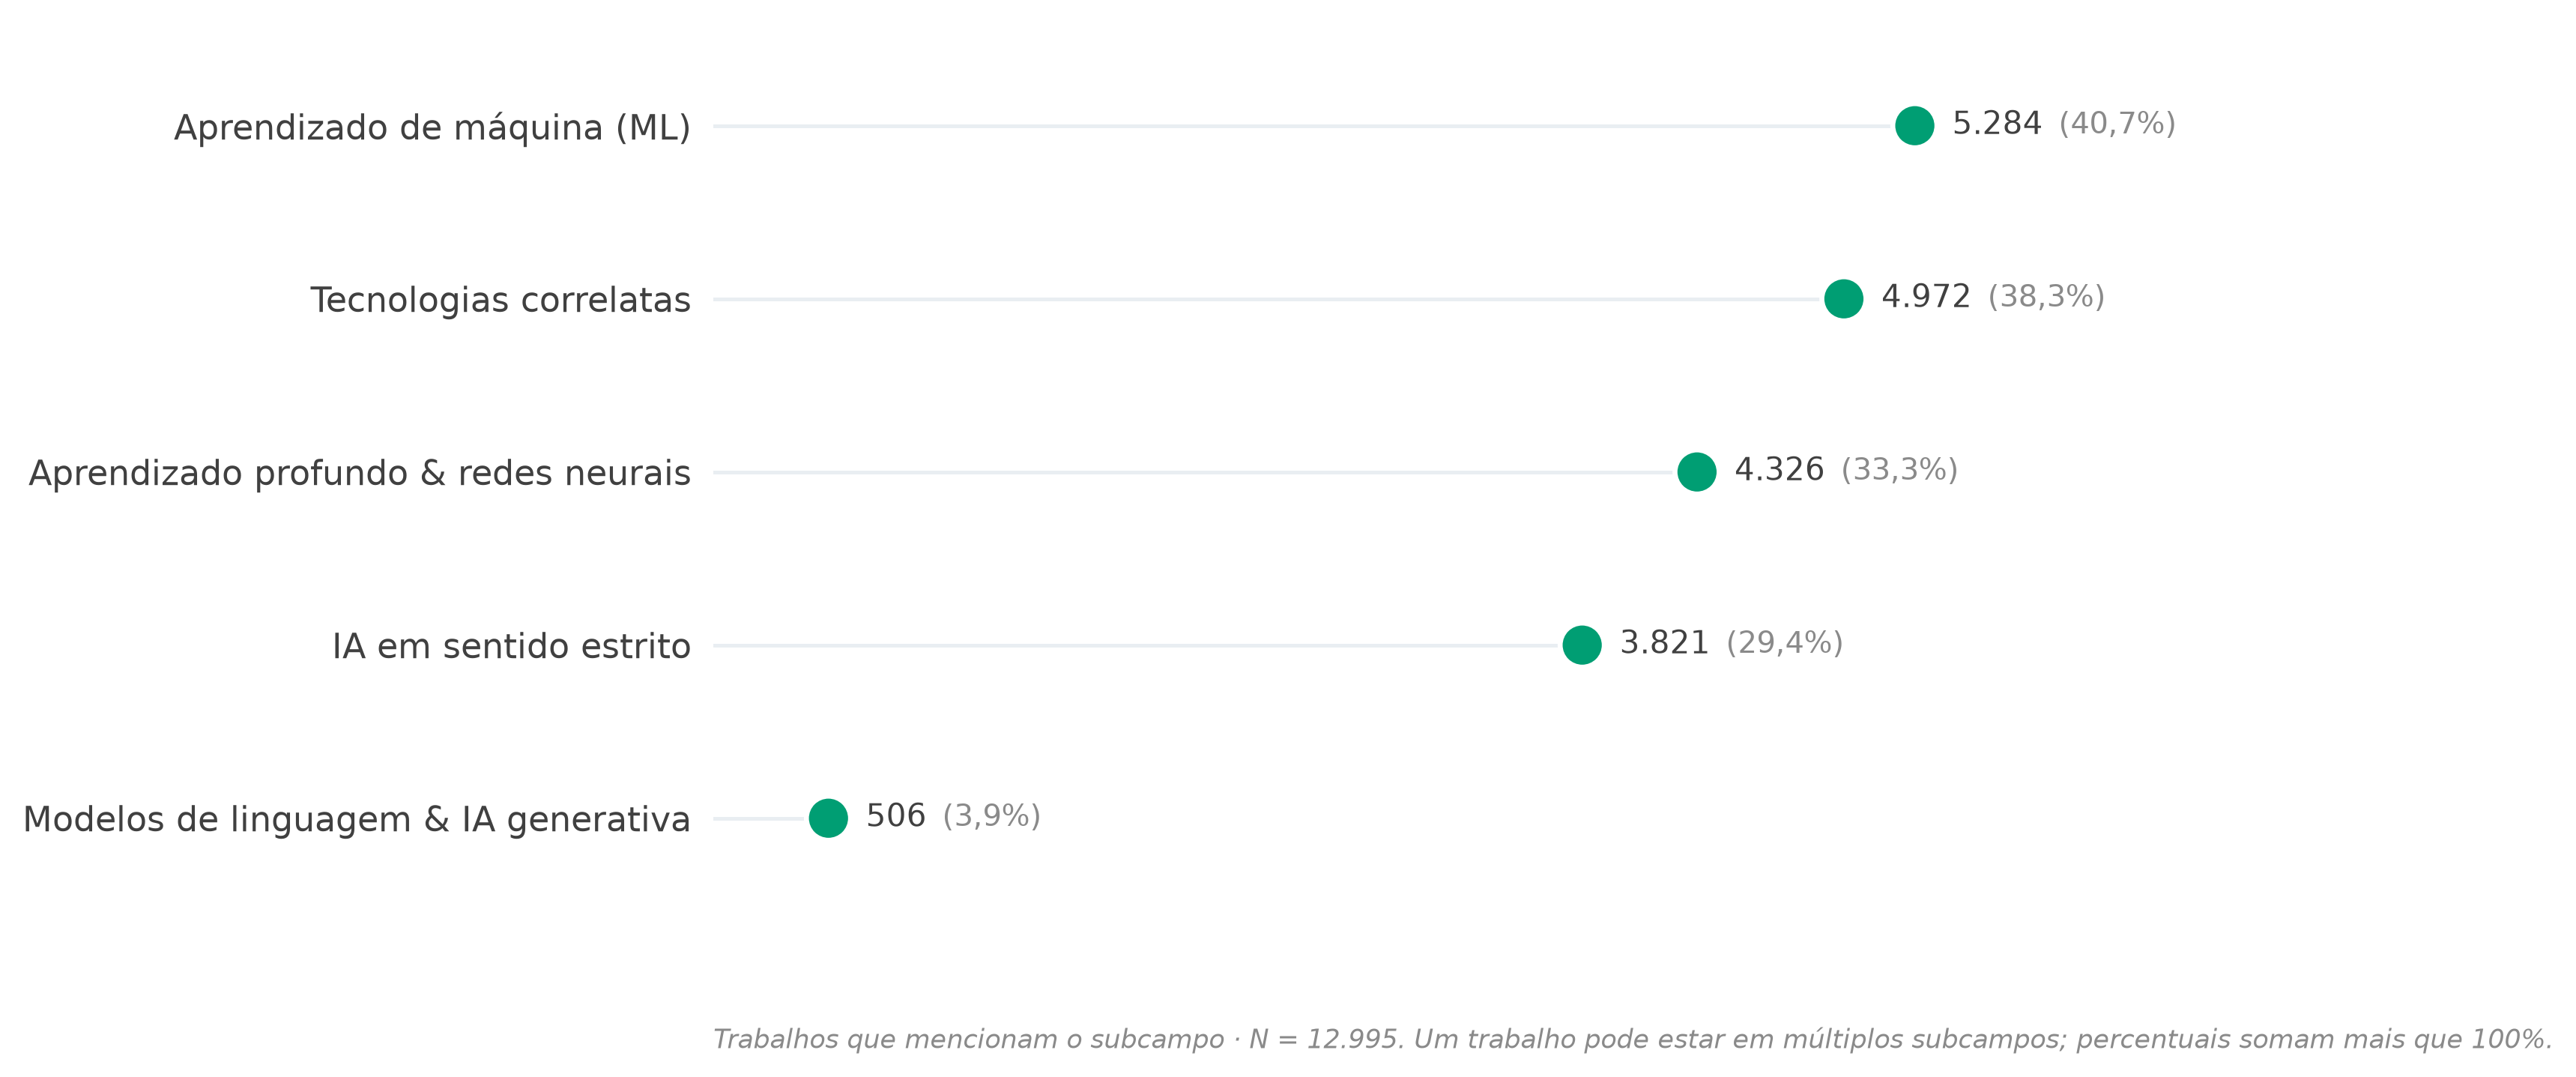
\includegraphics[width=0.85\linewidth]{figuras/cap.2/capes-scielo/capes_21_subcampos_distribuicao.png}
    \caption[Distribuição do corpus \texttt{Capes} por subcampo, 2021--2024]{%
        Distribuição das 12.995 defesas do corpus pelos cinco subcampos do
        classificador. Um mesmo trabalho pode pertencer a mais de um subcampo,
        e por isso a soma dos percentuais ultrapassa cem. O aprendizado de
        máquina é o subcampo mais frequente, com 5.284 defesas, seguido pelas
        tecnologias correlatas, com 4.972, e pelo aprendizado profundo e redes
        neurais, com 4.326, ao passo que a inteligência artificial em sentido
        estrito aparece só em quarto lugar, com 3.821, o que contraria
        a expectativa de que \enquote{inteligência artificial} seja o rótulo
        dominante. Os modelos de linguagem e a inteligência artificial
        generativa formam o menor subcampo em volume, com 506 defesas.
        Elaboração própria a partir do Catálogo de Teses e Dissertações da
        \texttt{Capes}, \emph{dump} oficial \texttt{BR-CAPES-BTD-2021A2024}.
        Dados de domínio público. Repositório com dados, \emph{scripts} e figuras em \protect\url{https://github.com/julianehelanski/bibliometria-ia-humanas}.}
    \label{fig:capes_subcampos}
\end{figure}

A distribuição dos cinco subcampos ao longo do quadriênio mostra um movimento que interessa de perto a esta tese. O aprendizado de máquina mantém-se como o subcampo de maior volume em todos os quatro anos, e os modelos de linguagem e a inteligência artificial generativa, embora sejam o menor subcampo em volume absoluto, apresentam o maior crescimento proporcional em 2024.\footnote{A figura que apresenta a evolução anual de cada um dos cinco subcampos no quadriênio fica versionada no repositório da análise bibliométrica, em \url{https://github.com/julianehelanski/bibliometria-ia-humanas}.} Esse salto é o corolário, na produção de pós-graduação brasileira, da popularização do \texttt{ChatGPT} a partir de novembro de 2022, e marca o momento em que a inteligência artificial generativa começa a ser absorvida como objeto de pesquisa pela pós-graduação do país.

Do universo de 350.071 trabalhos defendidos no quadriênio, 12.995 tocam o campo da inteligência artificial, do aprendizado de máquina ou do aprendizado profundo, o que corresponde a 3,71\% da produção nacional de pós-graduação. A Figura~\ref{fig:capes_grande_area} apresenta a distribuição desses 12.995 trabalhos pelas grandes áreas do conhecimento, e traz, além da participação de cada grande área no corpus de inteligência artificial, a taxa interna, isto é, o percentual da produção total de cada grande área que toca o campo.

\begin{figure}[htbp]
    \centering
    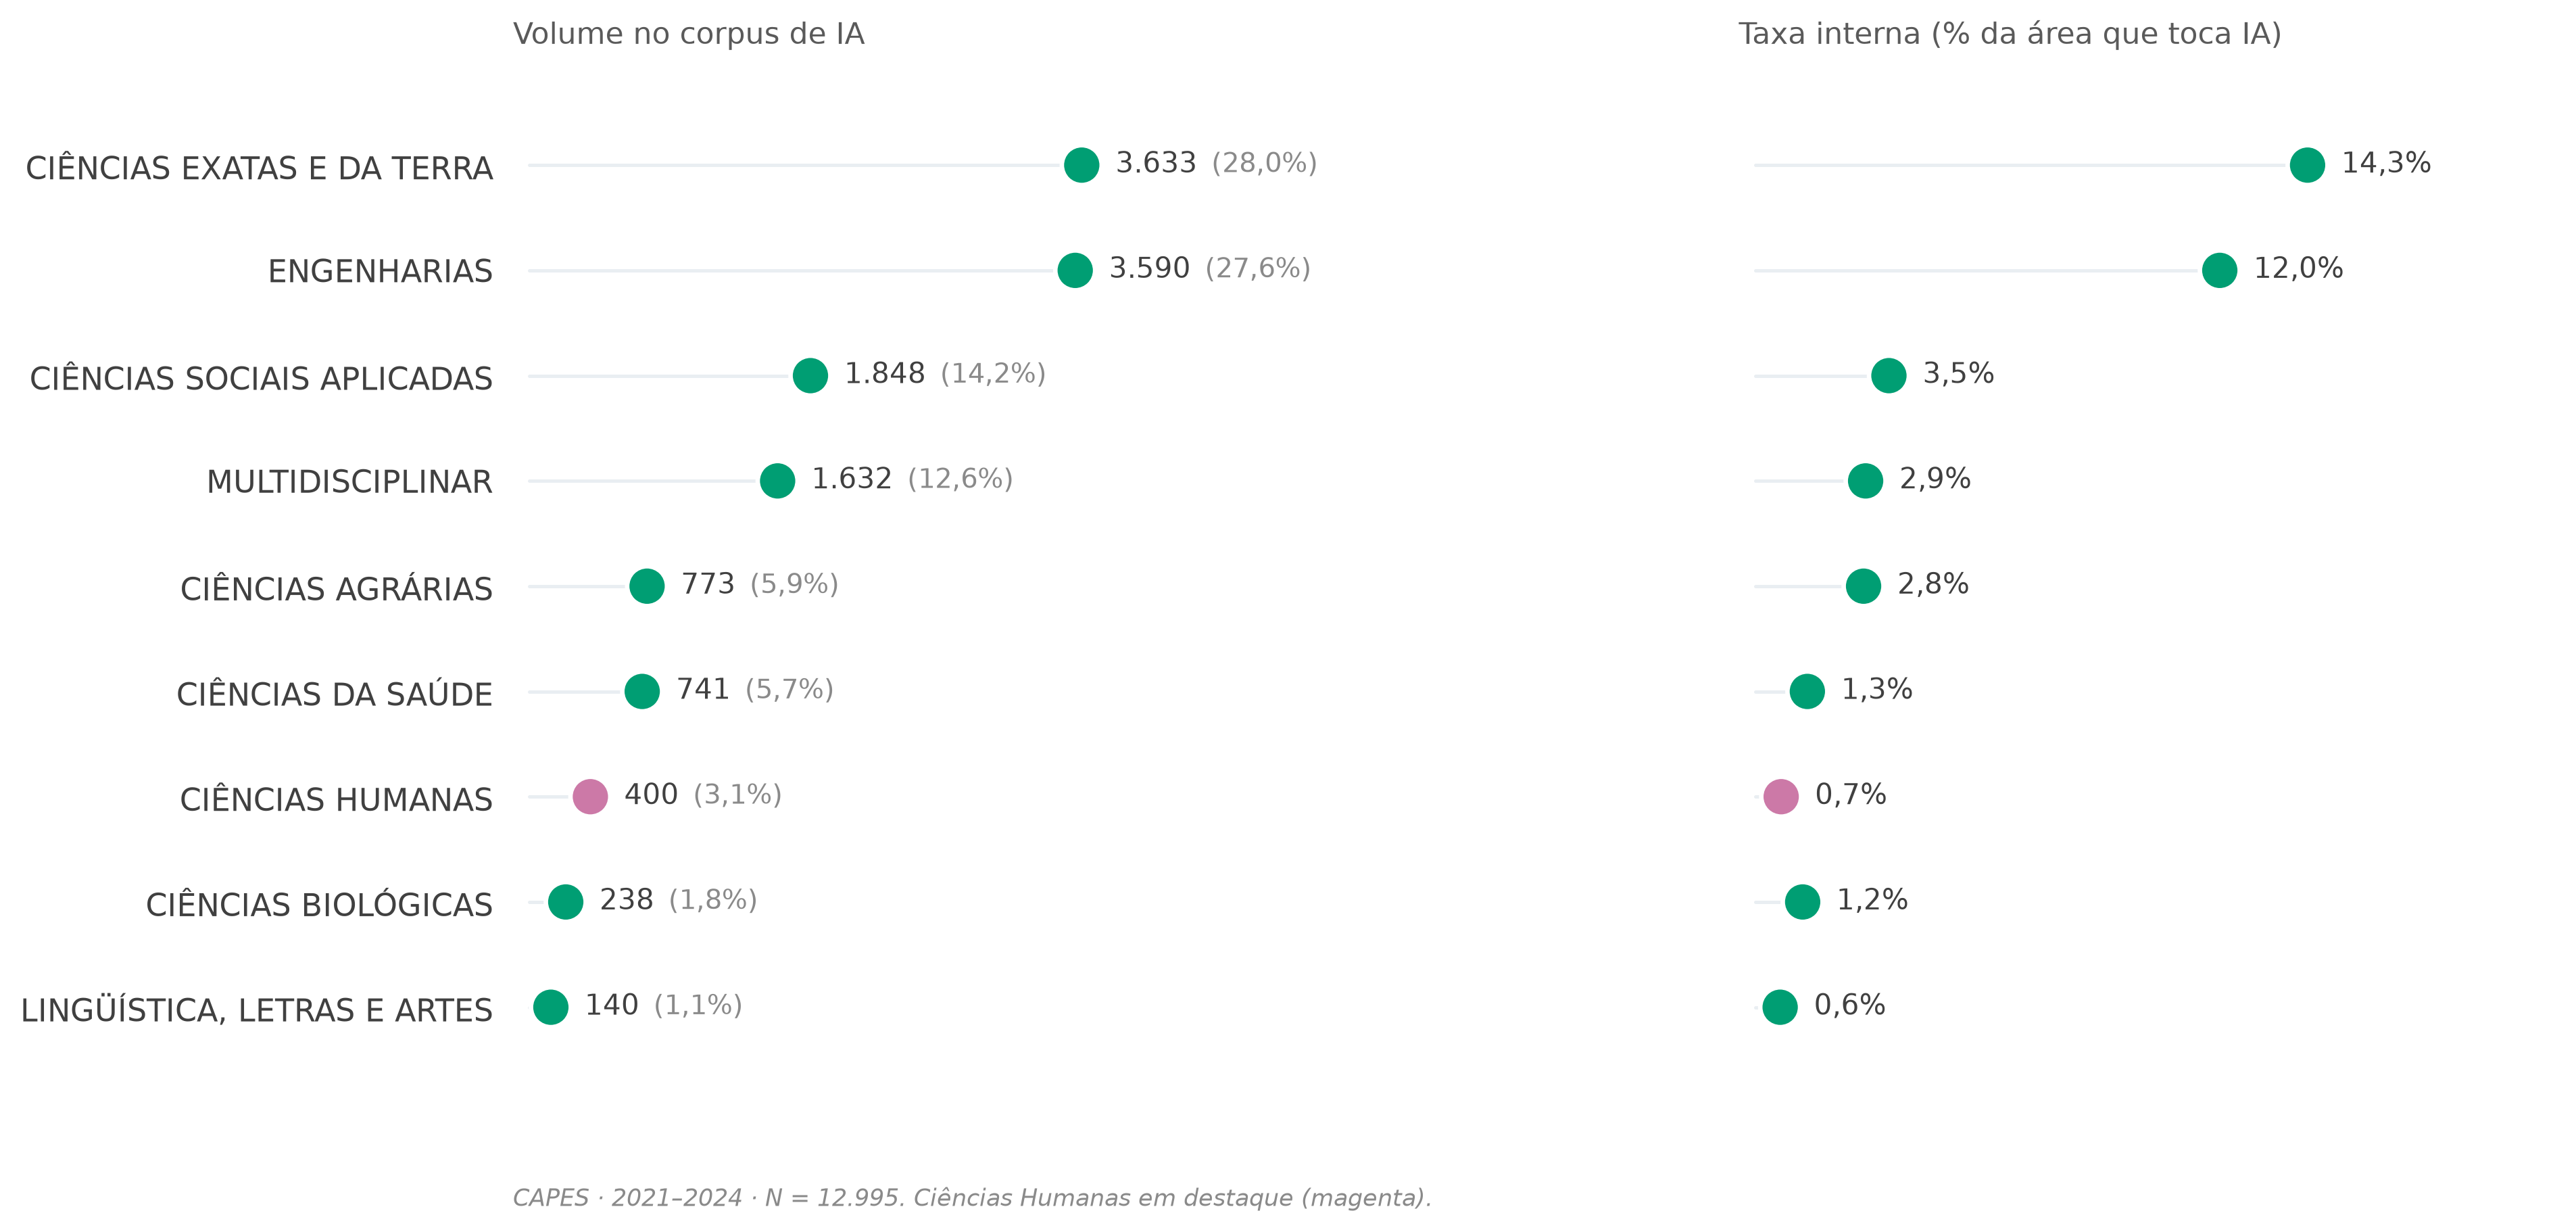
\includegraphics[width=0.95\linewidth]{figuras/cap.2/capes-scielo/capes_11_grande_area_share.png}
    \caption[Distribuição da produção sobre IA por grande área, \texttt{Capes} 2021--2024]{%
        Distribuição dos 12.995 trabalhos sobre inteligência artificial,
        aprendizado de máquina e aprendizado profundo defendidos na
        pós-graduação brasileira no quadriênio 2021--2024, por grande área de
        conhecimento. O painel da esquerda mostra o volume absoluto e a
        participação percentual no corpus, e o painel da direita mostra a taxa
        interna, isto é, a fração das defesas de cada grande área que tocam o
        campo. As Ciências Humanas, em destaque, são a maior grande área no
        universo total da pós-graduação brasileira, com 59.976 defesas no
        quadriênio, e ainda assim respondem por apenas 3,08\% do corpus de
        inteligência artificial, e somente 0,67\% das defesas em Ciências
        Humanas tocam o campo, contra 14,29\% nas Ciências Exatas e da Terra e
        12,01\% nas Engenharias. Elaboração própria a partir do Catálogo de
        Teses e Dissertações da \texttt{Capes}, \emph{dump} oficial
        \texttt{BR-CAPES-BTD-2021A2024}. Dados de domínio público. Repositório com dados, \emph{scripts} e figuras em \protect\url{https://github.com/julianehelanski/bibliometria-ia-humanas}.}
    \label{fig:capes_grande_area}
\end{figure}

A Figura~\ref{fig:capes_grande_area} permite ler a posição das Ciências Humanas em dois modos. No primeiro, as Ciências Humanas são a maior grande área do universo total da pós-graduação brasileira, com 59.976 trabalhos defendidos no quadriênio, e contribuem com apenas 3,08\% do corpus de inteligência artificial. No segundo, e a leitura que mais pesa para o argumento, apenas 0,67\% das defesas em Ciências Humanas tocam o campo da inteligência artificial, contra 12,01\% nas Engenharias e 14,29\% nas Ciências Exatas e da Terra, uma diferença de uma ordem de grandeza. As ciências humanas brasileiras se aproximam da inteligência artificial como objeto de pesquisa em um ritmo que é, em termos proporcionais, entre dezoito e vinte e uma vezes mais lento que o das engenharias e das ciências exatas.

A diferença entre as grandes áreas é de volume e de vocabulário. Quando cruzo os cinco subcampos com as nove grandes áreas, encontro o que chamo de assinatura discursiva de cada área, isto é, o conjunto de termos pelos quais cada grande área se aproxima do campo. O aprendizado profundo e as redes neurais concentram-se de modo quase exclusivo nas Ciências Exatas e nas Engenharias, e as Ciências Humanas, quando tocam o campo, tocam-no sobretudo pela inteligência artificial como conceito e pelas tecnologias correlatas, e quase nunca pelos termos técnicos. As Figuras~\ref{fig:capes_heatmap_keyword} e~\ref{fig:capes_heatmap_subcampo} apresentam esse cruzamento em dois recortes. A leitura das duas figuras sustenta um ponto que importa ao argumento desta tese: a inteligência artificial significa coisas distintas em áreas distintas, mesmo quando a soma agregada parece uniforme, e os modelos de linguagem e a inteligência artificial generativa são o subcampo que mais atravessa as fronteiras disciplinares, com presença que se espalha pelas Ciências Sociais Aplicadas, pela área Multidisciplinar e pelas Ciências Humanas, em lugar de se concentrar nas exatas. Quando uma defesa fora das ciências exatas toca o campo, é mais provável que o faça pela porta da inteligência artificial generativa do que pela das redes neurais, e esse achado é coerente com a hipótese que sustento sobre o \texttt{ChatGPT} como ponto de virada da entrada da inteligência artificial no discurso público e nas ciências humanas.

\begin{figure}[htbp]
    \centering
    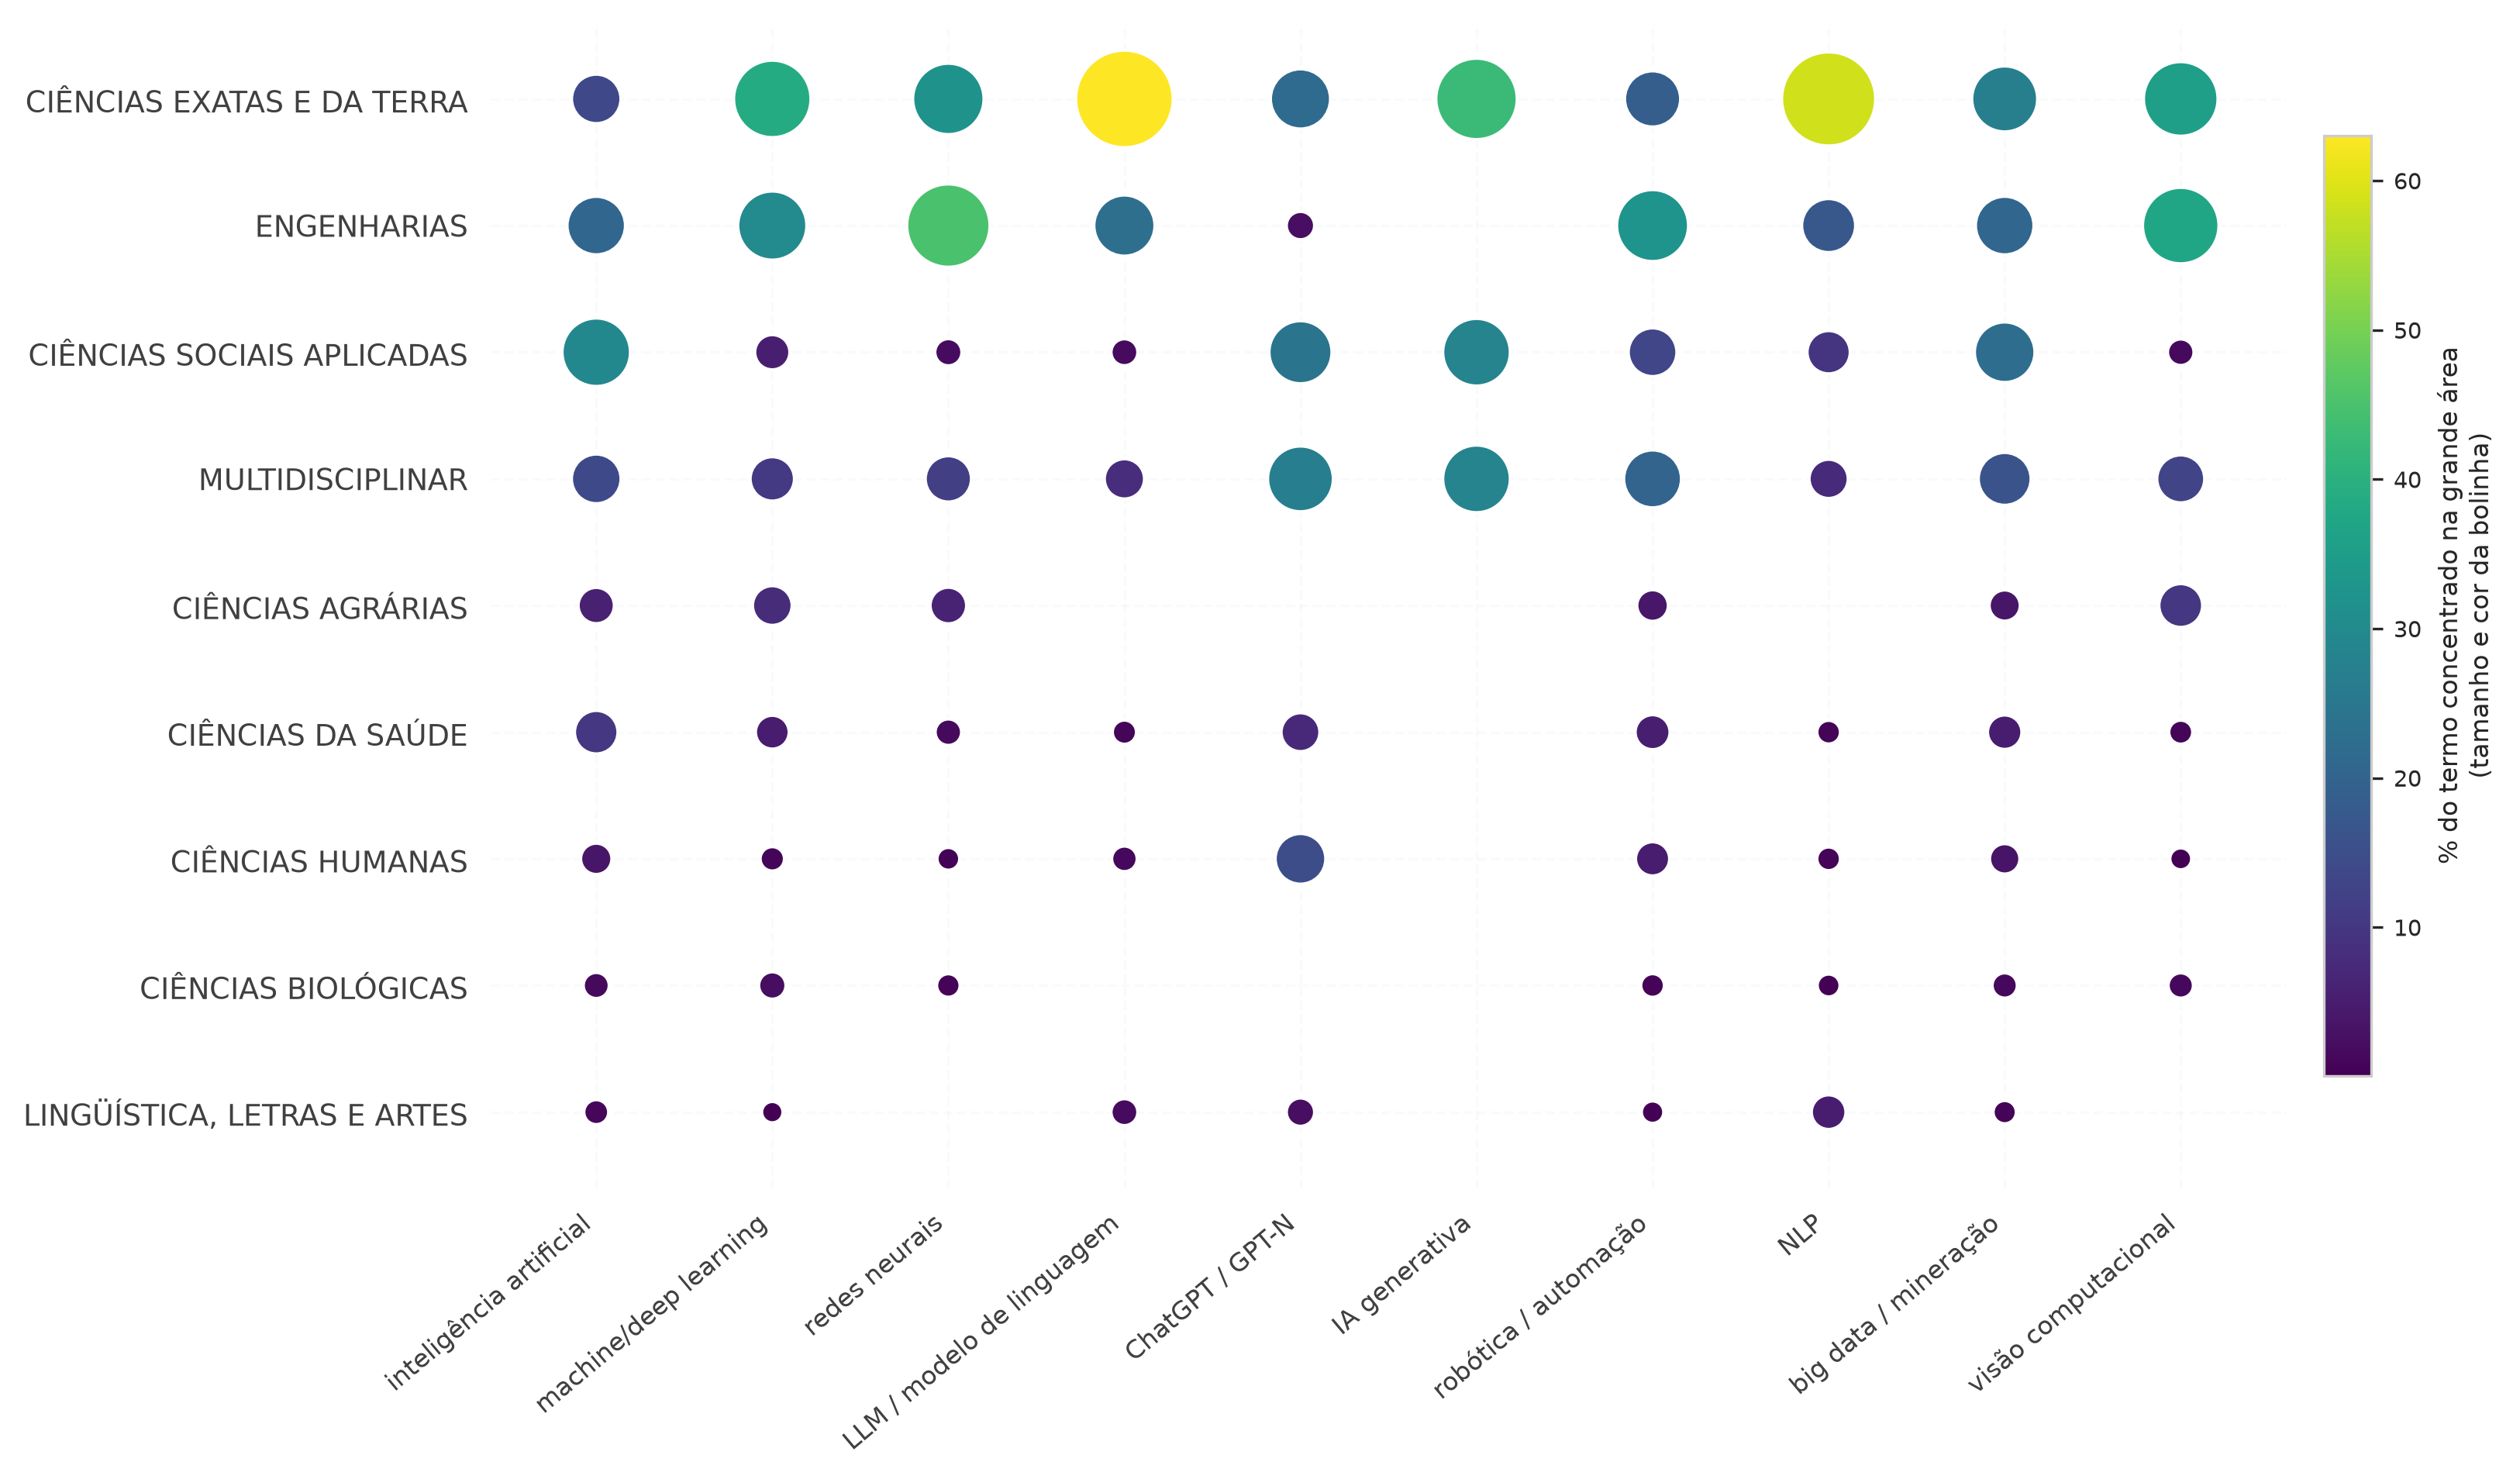
\includegraphics[width=0.95\linewidth]{figuras/cap.2/capes-scielo/capes_13_heatmap_area_keyword.png}
       \caption[Co-ocorrência entre termos-chave e grandes áreas, \texttt{Capes} 2021--2024]{%
        Matriz de bolhas da co-ocorrência entre dez termos-chave do campo e as
        nove grandes áreas de conhecimento da \texttt{Capes}, sobre o corpus de
        12.995 defesas. Em cada cruzamento, o tamanho e a cor da bolha indicam o
        percentual do termo da coluna que se concentra naquela grande área, numa
        escala sequencial branco-verde ancorada no verde Okabe-Ito, em matiz
        distinto do par azul-vermelho das matrizes de bolhas do
        capítulo~\ref{capitulo3}, segundo a colorbar à direita da figura. A
        leitura por coluna evidencia que termos como \enquote{redes neurais} e
        \enquote{aprendizado profundo} concentram-se nas Ciências Exatas e nas
        Engenharias, ao passo que \enquote{\texttt{ChatGPT}} distribui-se por
        todas as áreas, com presença nas Ciências Sociais Aplicadas e nas
        Ciências Humanas. Elaboração própria a partir do Catálogo de Teses e
        Dissertações da \texttt{Capes}, \emph{dump} oficial
        \texttt{BR-CAPES-BTD-2021A2024}. Dados de domínio público. Repositório
        com dados, \emph{scripts} e figuras em
        \protect\url{https://github.com/julianehelanski/bibliometria-ia-humanas}.}
    \label{fig:capes_heatmap_keyword}
\end{figure}

\begin{figure}[htbp]
    \centering
    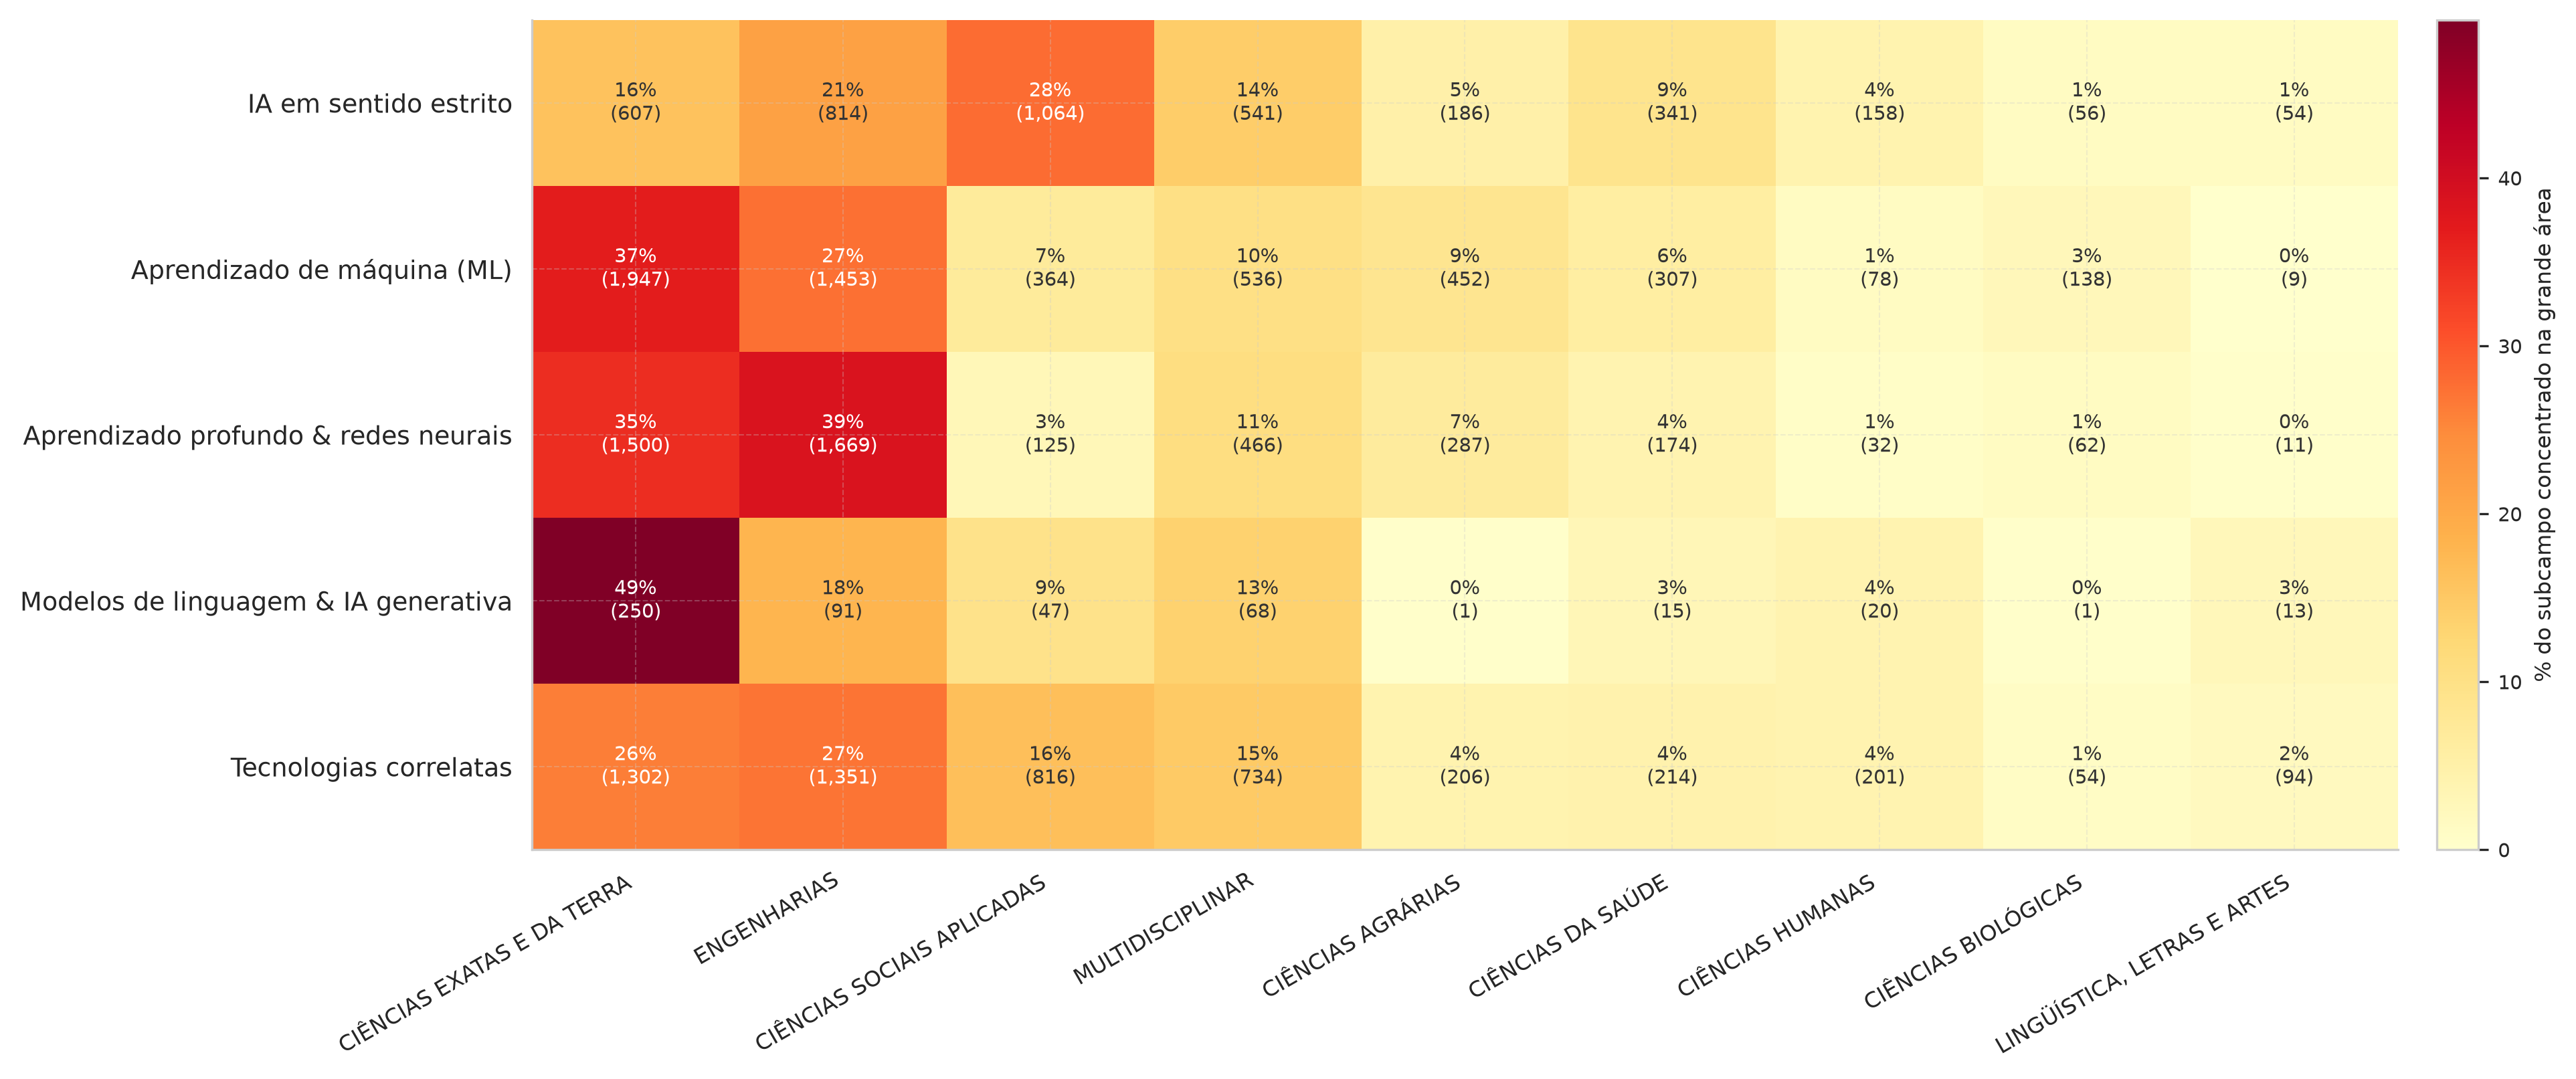
\includegraphics[width=0.95\linewidth]{figuras/cap.2/capes-scielo/capes_22_heatmap_subcampo_grande_area.png}
        \caption[Concentração dos subcampos por grande área, \texttt{Capes} 2021--2024]{%
        Matriz de bolhas da concentração dos cinco subcampos do classificador
        entre as nove grandes áreas. Cada linha, que corresponde a um subcampo,
        está normalizada para somar cem por cento, e mostra, para cada técnica,
        onde ela se concentra. Em cada cruzamento, o tamanho e a cor da bolha
        indicam o percentual do subcampo distribuído naquela grande área, numa
        escala sequencial branco-laranja ancorada no laranja Okabe-Ito, em
        matiz distinto do verde da Figura~\ref{fig:capes_heatmap_keyword} e
        do par azul-vermelho das matrizes de bolhas do
        capítulo~\ref{capitulo3}, segundo a colorbar à direita da figura. O
        aprendizado profundo e as redes neurais concentram-se nas Ciências
        Exatas e nas Engenharias, e os modelos de linguagem e a inteligência
        artificial generativa distribuem-se de modo mais espalhado, com
        presença nas Ciências Sociais Aplicadas, na área Multidisciplinar e
        nas Ciências Humanas. Elaboração própria a partir do Catálogo de Teses
        e Dissertações da \texttt{Capes}, \emph{dump} oficial
        \texttt{BR-CAPES-BTD-2021A2024}. Dados de domínio público. Repositório
        com dados, \emph{scripts} e figuras em
        \protect\url{https://github.com/julianehelanski/bibliometria-ia-humanas}.}
    \label{fig:capes_heatmap_subcampo}
\end{figure}

Os 400 trabalhos das Ciências Humanas que tocam o campo distribuem-se de modo desigual pelas áreas de conhecimento da grande área. A Figura~\ref{fig:capes_humanas_area} apresenta essa distribuição.

\begin{figure}[htbp]
    \centering
    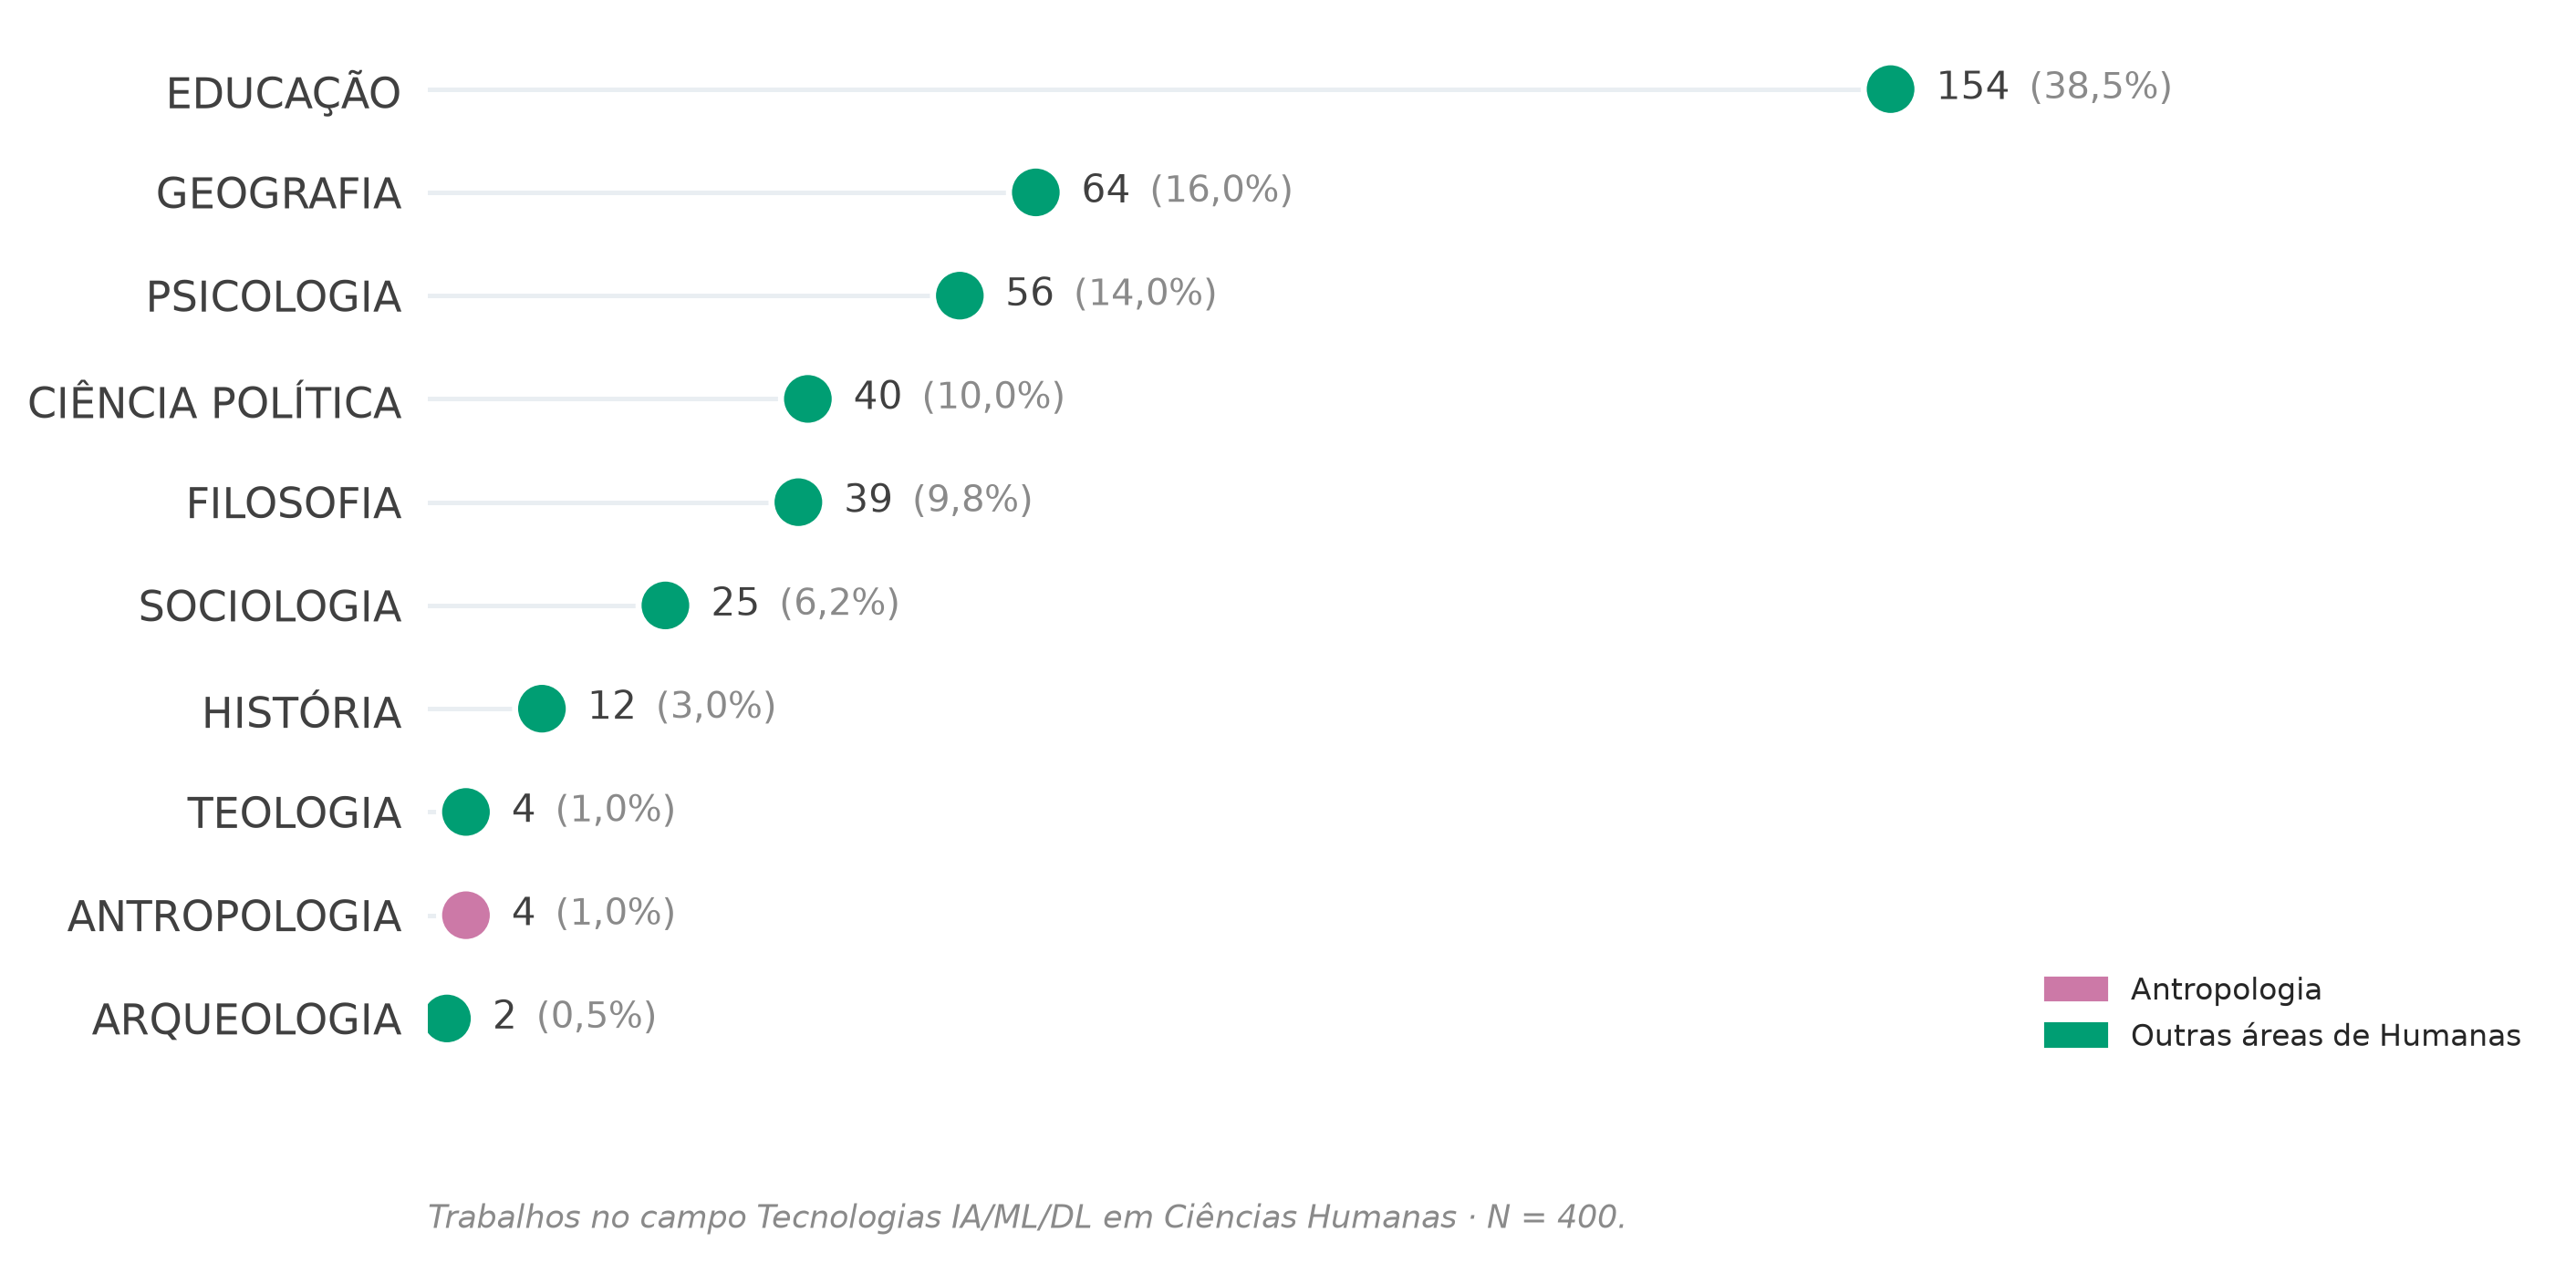
\includegraphics[width=0.85\linewidth]{figuras/cap.2/capes-scielo/capes_h01_areas_humanas.png}
    \caption[Produção sobre IA nas Ciências Humanas por área, \texttt{Capes} 2021--2024]{%
        Distribuição das 400 defesas sobre inteligência artificial, aprendizado
        de máquina e aprendizado profundo na grande área de Ciências Humanas
        (2021--2024), por área de conhecimento. A Educação responde por 38,5\%
        das defesas, e é seguida de longe pela Geografia, com 16,0\%, e pela
        Psicologia, com 14,0\%. A Antropologia, em destaque, aparece com quatro
        defesas, 1,0\% do total, e ocupa a penúltima posição, à frente apenas
        da Arqueologia. A figura permite ler a marginalidade da Antropologia em
        duas camadas: a inteligência artificial é objeto periférico dentro das
        Ciências Humanas, e a Antropologia é periférica dentro desse recorte já
        periférico. Elaboração própria a partir do Catálogo de Teses e
        Dissertações da \texttt{Capes}, \emph{dump} oficial
        \texttt{BR-CAPES-BTD-2021A2024}. Dados de domínio público. Repositório com dados, \emph{scripts} e figuras em \protect\url{https://github.com/julianehelanski/bibliometria-ia-humanas}.}
    \label{fig:capes_humanas_area}
\end{figure}

A Educação concentra 38,5\% da produção de inteligência artificial em Ciências Humanas, e é seguida de longe pela Geografia e pela Psicologia. As três disciplinas que compõem o que costumo chamar de ciências sociais em sentido estrito, a Ciência Política, a Sociologia e a Antropologia, somam 69 das 400 defesas. A Antropologia registra quatro defesas sobre inteligência artificial no quadriênio 2021--2024 pela área de conhecimento da \texttt{Capes}; pela taxonomia de avaliação da agência, que agrupa Antropologia e Arqueologia em uma única área administrativa, são seis defesas.\footnote{A \texttt{Capes} classifica cada trabalho por dois critérios distintos, registrados em colunas separadas do \emph{dump} oficial. A área de conhecimento (\texttt{NM\_AREA\_CONHECIMENTO}) é o recorte disciplinar estrito, e nela a Antropologia tem quatro defesas e a Arqueologia tem duas. A área de avaliação (\texttt{NM\_AREA\_AVALIACAO}) é o recorte do organograma administrativo, pelo qual os programas de pós-graduação são de fato agrupados pela agência, e nela Antropologia e Arqueologia formam uma única área com seis defesas. Adoto os dois números porque a marginalidade que descrevo independe do critério: quatro ou seis, frente às 154 defesas da Educação ou às 64 da Geografia, sustentam a mesma leitura. As contagens das duas colunas, lidas diretamente da planilha, fecham em 400 em ambos os recortes, e ficam versionadas no arquivo \texttt{docs/decisoes\_metodologicas.md} do repositório.} Pela área de conhecimento, a Antropologia é a penúltima da figura, à frente apenas da Arqueologia. A posição da Antropologia se lê, assim, em camadas: a inteligência artificial é marginal no conjunto das Ciências Humanas, com 0,67\% da produção da grande área, e a Antropologia é marginal dentro desse conjunto já marginal, com 1,0\% das 400 defesas de inteligência artificial em Ciências Humanas. Quatro trabalhos em quatro anos, frente aos 154 da Educação ou aos 64 da Geografia, é uma densidade que situa minha tese no início dos estudos antropológicos brasileiros sobre inteligência artificial.

Na Antropologia, quatro defesas em quatro anos é pouco, e, ao ler caso a caso, verifico que esses quatro trabalhos, retornados pela classificação automática, não correspondem a quatro etnografias da inteligência artificial em específico. Das quatro defesas, duas tomam a inteligência artificial como objeto etnográfico em sentido estrito. A dissertação de Rafael Damasceno Ramalho Pereira, \textit{O problema das outras mentes: uma antropologia das inteligências artificiais}, defendida na \texttt{UFRJ} em 2021 sob orientação de Eduardo Viveiros de Castro, coloca o problema da simulação da mente diante do conceito antropológico de cultura para constituir o campo de uma antropologia das inteligências artificiais, e busca um caminho que escape tanto ao cognitivismo das ciências exatas quanto à genealogia do poder das ciências sociais, com a conclusão de que as concepções de inteligência que respaldam esses projetos vêm acopladas a uma despolitização do espírito. A dissertação de Louise Lima Karczeski, \textit{Gerando inteligência: considerações etnográficas sobre a construção de objetividade no campo da inteligência artificial}, defendida na \texttt{UFSC} em 2022 sob orientação de Leticia Cesarino, acompanha em conferências, cursos e comunidades on-line os especialistas que elaboram modelos de inteligência artificial, e descreve como eles reivindicam a objetividade de suas aplicações por três enquadres, o mercado, a ciência e a ética; é, das quatro, a mais próxima do que faço nesta tese. As outras duas defesas tocam o campo de modo oblíquo: a tese de Isabel Wittmann, \textit{Feminilidades maquínicas: gênero, sexualidade e corpo de mulheres artificiais no cinema fantástico}, defendida na \texttt{USP} em 2023 sob orientação de Rose Satiko Gitirana Hikiji, traça uma genealogia das mulheres artificiais no cinema, de \textit{Metrópolis} a \textit{Ex Machina}, e aciona androides, robôs e ciborgues como figuras culturais à luz das teóricas feministas do cinema, em lugar de tomar um sistema técnico como objeto; e a dissertação de Fabricio Bernardes, \textit{Gerenciamento de dados arqueológicos digitais: estudo de caso a partir da região estuarina do município de Rio Grande, Rio Grande do Sul, Brasil}, defendida na \texttt{UFPel} em 2023 sob orientação de Rafael Guedes Milheira, avalia a curadoria e o reaproveitamento dos dados arqueológicos do \texttt{IPHAN} pelos conceitos de inventário patrimonial, ciberinfraestrutura e \emph{big data}, e foi retornada pelo classificador por tocar o subcampo das tecnologias correlatas, sem ser uma pesquisa sobre inteligência artificial. A distância entre os quatro trabalhos retornados pelo classificador e as duas etnografias que de fato tomam a inteligência artificial como objeto é o tipo de distinção que a classificação automática não faz, e que a leitura situada precisa fazer.\footnote{A triagem de auditoria é a leitura caso a caso que faço sobre o resultado do \emph{regex} de cinco subcampos em cada recorte disciplinar, e o seu princípio vale para além do caso da Antropologia. O \emph{regex} detecta a presença de um termo, e não o uso que o trabalho faz dele, e por isso gera dois tipos de falso positivo. O primeiro é o trabalho que menciona um termo do campo como contexto ou horizonte, sem que a inteligência artificial seja seu objeto. O segundo é o trabalho que aplica uma técnica de aprendizado de máquina como método, em que a inteligência artificial entra como instrumento e não como objeto da pesquisa, como nas defesas de Ciência Política que preveem a qualidade de medicamentos ou recomendam ações parlamentares. A planilha de auditoria por registro, com a classificação de cada trabalho, fica versionada no repositório para conferência e discussão.}

A Sociologia e a Ciência Política aparecem ao campo em número maior que a Antropologia, com 25 e 40 defesas respectivamente, e, ao ler os dois conjuntos, identifico que cada disciplina se aproxima da inteligência artificial por caminhos próprios. Na Sociologia, das 25 defesas, dezesseis tocam o subcampo das tecnologias correlatas, e o conjunto se organiza em boa parte em torno de temas como trabalho, plataformas e datificação. Entre esses temas, objetos de pesquisa como a automação na indústria farmacêutica de Anápolis, a automação do atendimento nos supermercados de Fortaleza, a reestruturação do trabalho bancário, o trabalho de entregadores por aplicativo no capitalismo de plataforma, o teletrabalho no \texttt{INSS} durante a pandemia, a transição das estatísticas oficiais para um regime de dataficação. Outras defesas desse subconjunto seguem para as redes sociais e a circulação de dados em chave política, com estudos sobre a \enquote{fala do crime} no Facebook, os grupos bolsonaristas no WhatsApp, o \emph{big data} no 7 de setembro de 2021 e o uso de tecnologias emergentes pelas forças de segurança do Ceará, ao lado de entradas mais dispersas sobre tecnologia espacial e o \texttt{INPE}, o mercado de automóveis, os \emph{chatbots} no contexto comercial e o patrocínio empresarial na arte contemporânea. A inteligência artificial aparece à Sociologia brasileira no contexto da transformação do trabalho e do mundo digital. Um caso destoa do conjunto e interessa a esta tese, a dissertação de João Ricardo Penteado Lopes da Silva, \textit{Tendências das políticas do Estado brasileiro para o desenvolvimento da inteligência artificial: o caso dos centros de pesquisa aplicada em inteligência artificial}, defendida na \texttt{UFC} em 2022 sob orientação de Edemilson Cruz Santana Junior, toma como objeto centros de pesquisa aplicada como o \texttt{C4AI}. Na Ciência Política e nas Relações Internacionais, das 40 defesas, um primeiro conjunto se organiza em torno da geopolítica, da defesa e da segurança, e varia entre temas como a competição estratégica entre Estados Unidos e China pela liderança em inteligência artificial, a disputa em torno da Huawei e do 5G, os drones e as embarcações autônomas, a guerra cognitiva nas redes sociais, e também temas como \emph{big data} no policiamento da Polícia Militar de Minas Gerais. Um segundo conjunto vem da administração pública e do poder legislativo, e parte da inteligência artificial na gestão estatal, como a inteligência artificial no judiciário e na gestão de acervo processual, na avaliação de políticas públicas, no combate ao sobrepreço nas compras públicas, na regulação das consultas normativas da Anatel e na comunicação política dos senadores nas redes. Uma parte dessas defesas, ademais, não toma a inteligência artificial por objeto, e a usa como método de análise por aprendizado de máquina, em temas mais específicos como a predição da qualidade de medicamentos e a recomendação de ações parlamentares e de padrões de carreira parlamentar.

A distribuição temporal dos 400 trabalhos de inteligência artificial em Ciências Humanas mostra uma curva de aceleração: 69 defesas em 2021, 81 em 2022, 108 em 2023 e 142 em 2024. A produção mais que dobrou no intervalo de quatro anos, e a aceleração é coerente com a popularização da inteligência artificial generativa a partir do final de 2022. A Figura~\ref{fig:capes_temporal} apresenta essa curva.

\begin{figure}[htbp]
    \centering
    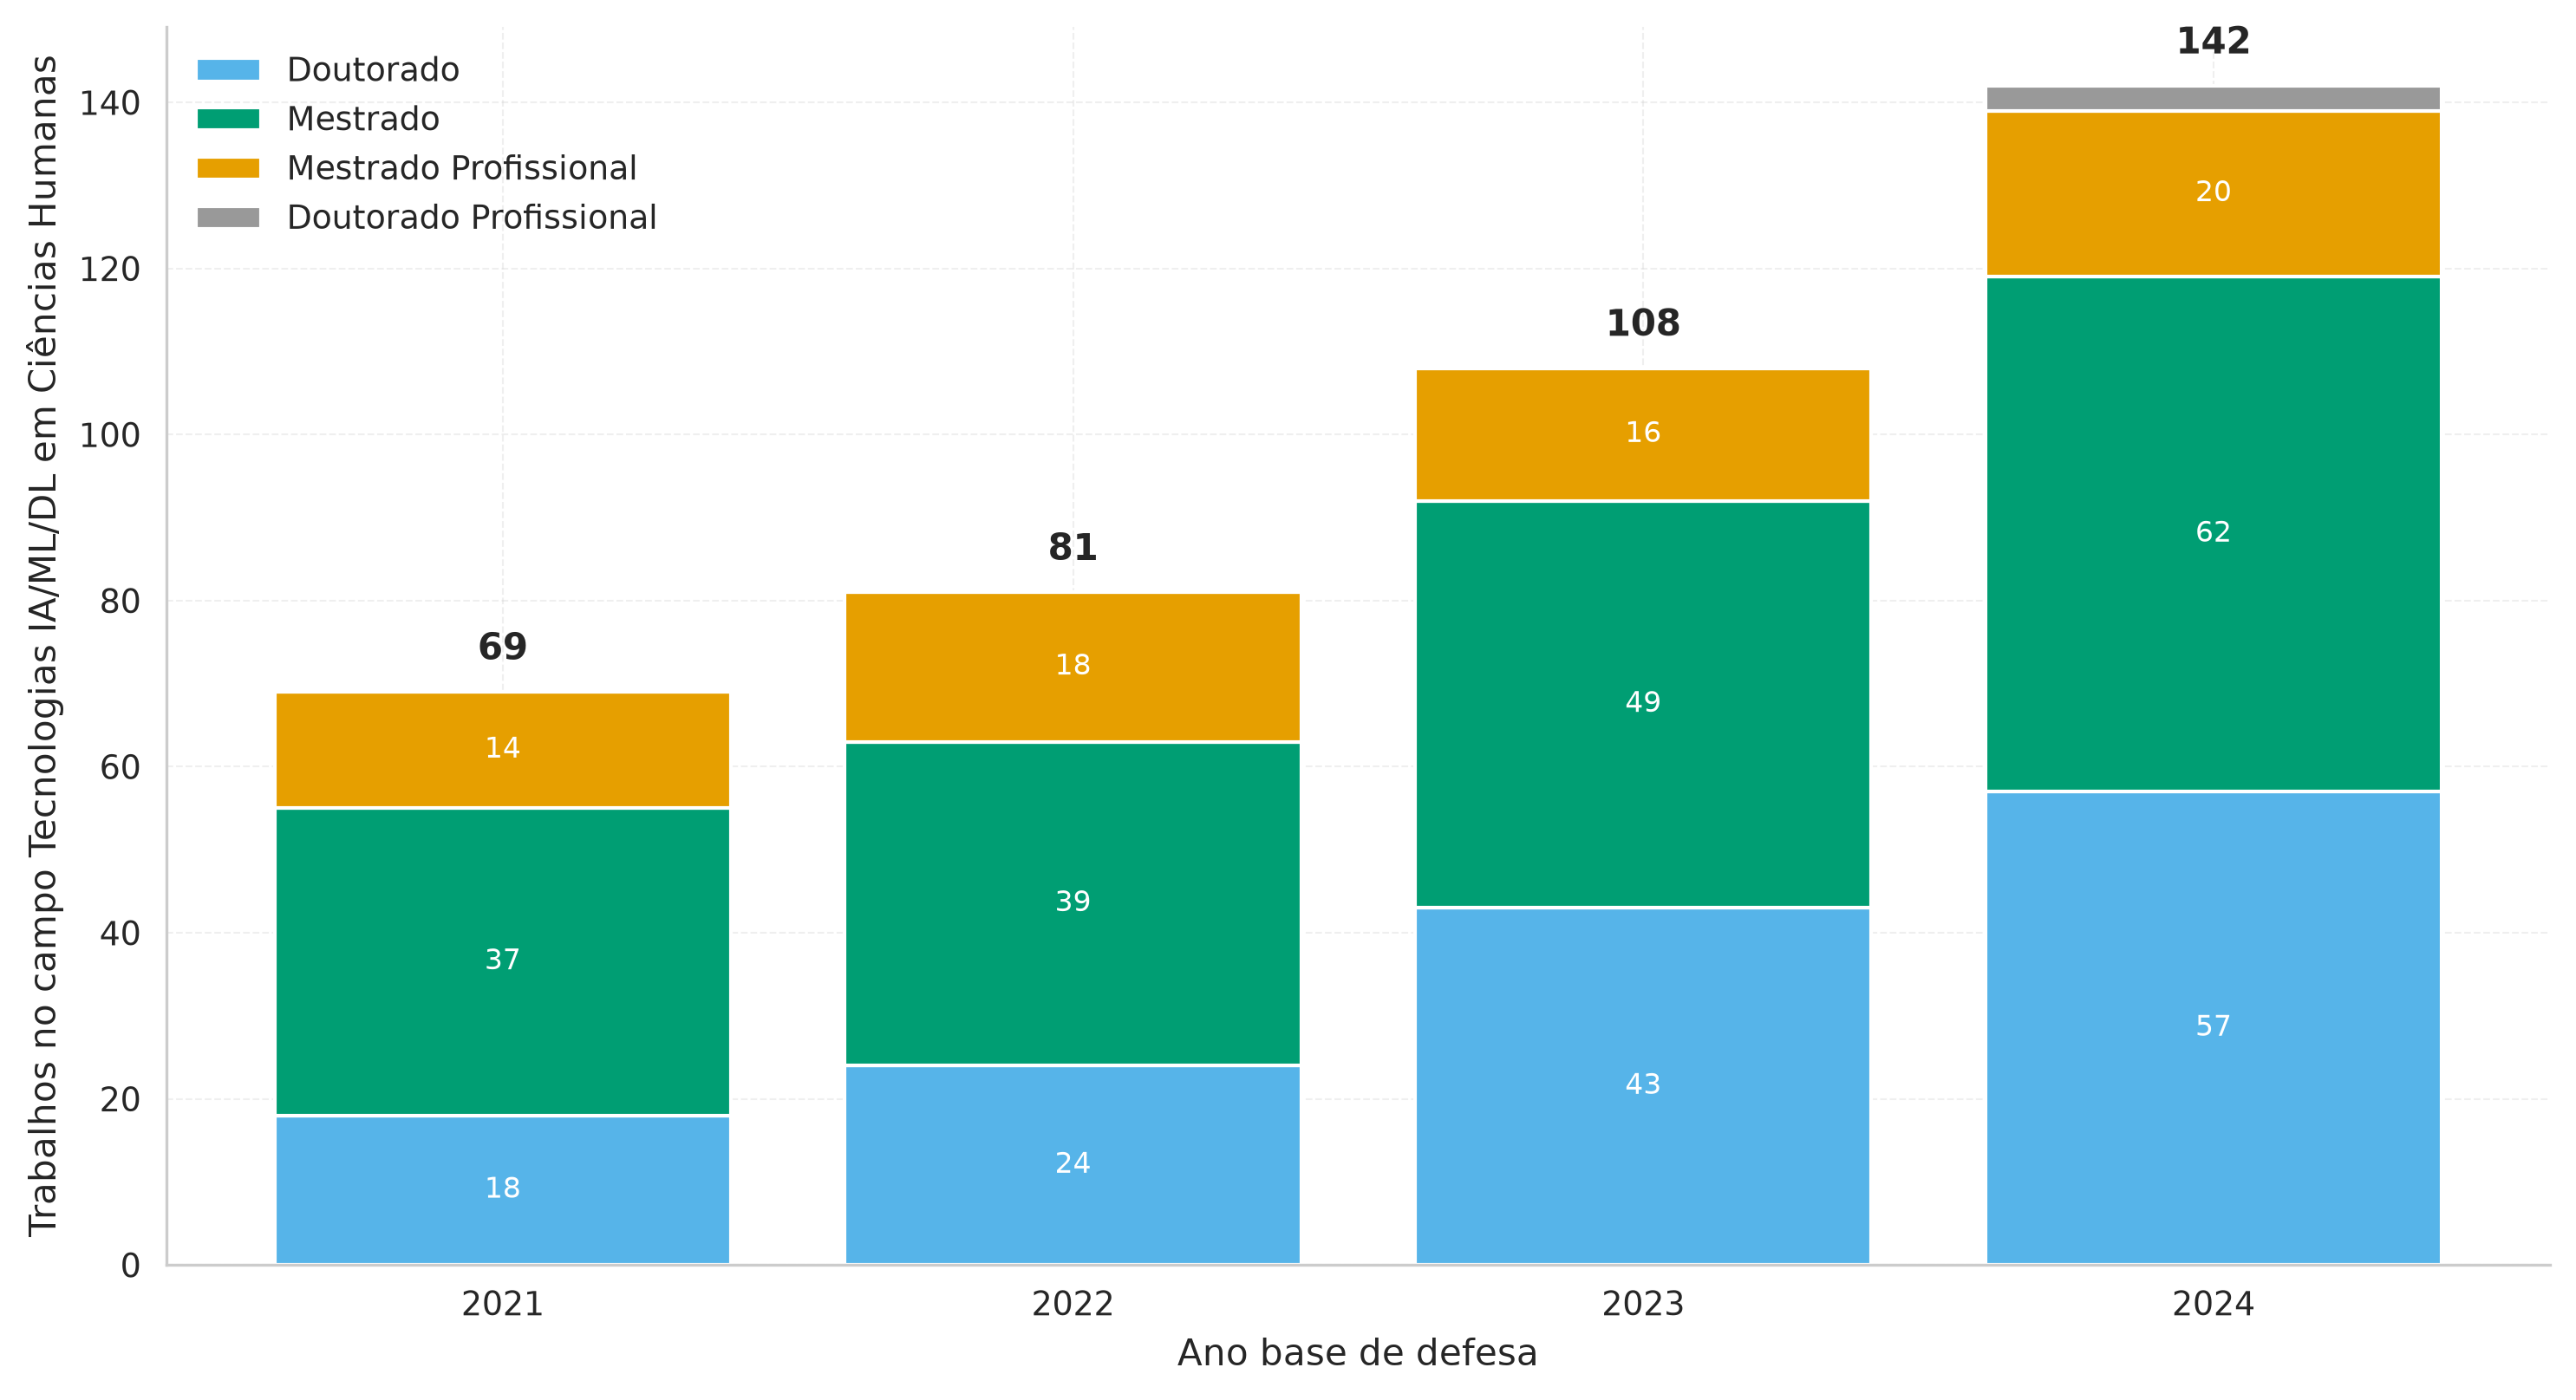
\includegraphics[width=0.85\linewidth]{figuras/cap.2/capes-scielo/capes_h02_temporal_humanas.png}
    \caption[Evolução temporal da produção sobre IA nas Ciências Humanas, \texttt{Capes} 2021--2024]{%
        Evolução anual das defesas em Ciências Humanas no campo da inteligência
        artificial, do aprendizado de máquina e do aprendizado profundo
        (2021--2024), em uma linha por grau acadêmico. O conjunto cresce de 69
        defesas em 2021 para 142 em 2024, mais que o dobro no intervalo de
        quatro anos, e o Mestrado responde pela maior parte do crescimento. A
        curva indica que as Ciências Humanas se aproximam do campo a partir de
        uma base reduzida, e que a marginalidade que descrevo é o estado
        presente de um campo em formação, em lugar de uma tendência estática.
        Elaboração própria a partir do Catálogo de Teses e Dissertações da
        \texttt{Capes}, \emph{dump} oficial \texttt{BR-CAPES-BTD-2021A2024}.
        Dados de domínio público. Repositório com dados, \emph{scripts} e figuras em \protect\url{https://github.com/julianehelanski/bibliometria-ia-humanas}.}
    \label{fig:capes_temporal}
\end{figure}

A segunda base do mapeamento é a coleção brasileira da biblioteca eletrônica \texttt{SciELO}, que indexa o artigo publicado em periódico. Coletei o corpus \texttt{SciELO} pela \emph{API} ArticleMeta. Uma \emph{API} (\emph{Application Programming Interface}, ou interface de programação de aplicações) é um canal pelo qual um sistema disponibiliza seus dados de modo estruturado, para que outro programa os requisite de forma automatizada, em lugar da navegação manual pela página \emph{web}. No caso da \texttt{SciELO}, a \emph{API} ArticleMeta devolve os metadados de cada artigo da coleção, como título, autoria, ano, periódico e área, em formato legível por máquina, e foi por ela que requisitei o corpus.\footnote{A \emph{API} ArticleMeta é o serviço de acesso programático aos metadados da rede \texttt{SciELO}, mantido pela própria plataforma. Requisitei o corpus com o \texttt{claude code} no terminal, em sessões iteradas de requisição, classificação e auditoria, e versionei o \emph{cache} completo da coleta no repositório. A \emph{API} delimita a janela temporal pela data de indexação do artigo na plataforma, e não pela data de publicação, e por isso a coleta bruta retornou artigos fora do quadriênio: dos 659 artigos no campo da inteligência artificial retornados sem filtro de ano, 28 foram publicados fora de 2021--2024 e ficam descartados de todas as análises desta seção. Os dados da \texttt{SciELO} são dinâmicos, e consultas futuras podem apresentar resultados distintos. Os números canônicos das duas bases, e a proveniência de cada um, ficam versionados no arquivo \texttt{docs/decisoes\_metodologicas.md} do repositório.} A coleta bruta retornou 98.165 artigos da coleção brasileira, e o recorte estrito ao quadriênio 2021--2024, por ano de publicação, delimita o universo de 90.360 artigos sobre o qual calculo as taxas internas. Apliquei a esse universo o mesmo \emph{regex} de cinco subcampos que apliquei ao Catálogo da \texttt{Capes}, e o classificador identificou 631 artigos no campo da inteligência artificial, do aprendizado de máquina e do aprendizado profundo. Dos 631 artigos do recorte, 225 foram publicados em 2024 contra 107 em 2021, crescimento que registra, na produção publicada em periódico, a mesma aceleração recente que a \texttt{Capes} mostra na produção de pós-graduação.

A Figura~\ref{fig:scielo_subject_area} apresenta a distribuição dos 631 artigos pelas oito \emph{subject\_areas} da coleção, mais a categoria Multidisciplinar que reúne os periódicos de classificação múltipla, com a taxa interna de cada uma.\footnote{O \texttt{SciELO} classifica seus periódicos em oito \emph{subject\_areas} canônicas. A categoria Multidisciplinar não é uma delas: agrupa os periódicos cuja classificação lista mais de uma área, e a mantenho como categoria sintética do meu procedimento de classificação. A taxa interna de uma área é a fração dos artigos dessa área que tocam o campo da inteligência artificial, isto é, o número de artigos da área no campo dividido pelo total de artigos que a área publicou no quadriênio. Por usar como base o universo de cada área, e não o volume absoluto, a taxa interna permite comparar a densidade do tema entre áreas de tamanhos distintos: a Engenharia publica menos que as Ciências da Saúde em número absoluto de artigos sobre inteligência artificial, e ainda assim apresenta a maior taxa interna, porque a inteligência artificial ocupa uma fração maior do que a Engenharia publica.}

\begin{figure}[htbp]
    \centering
    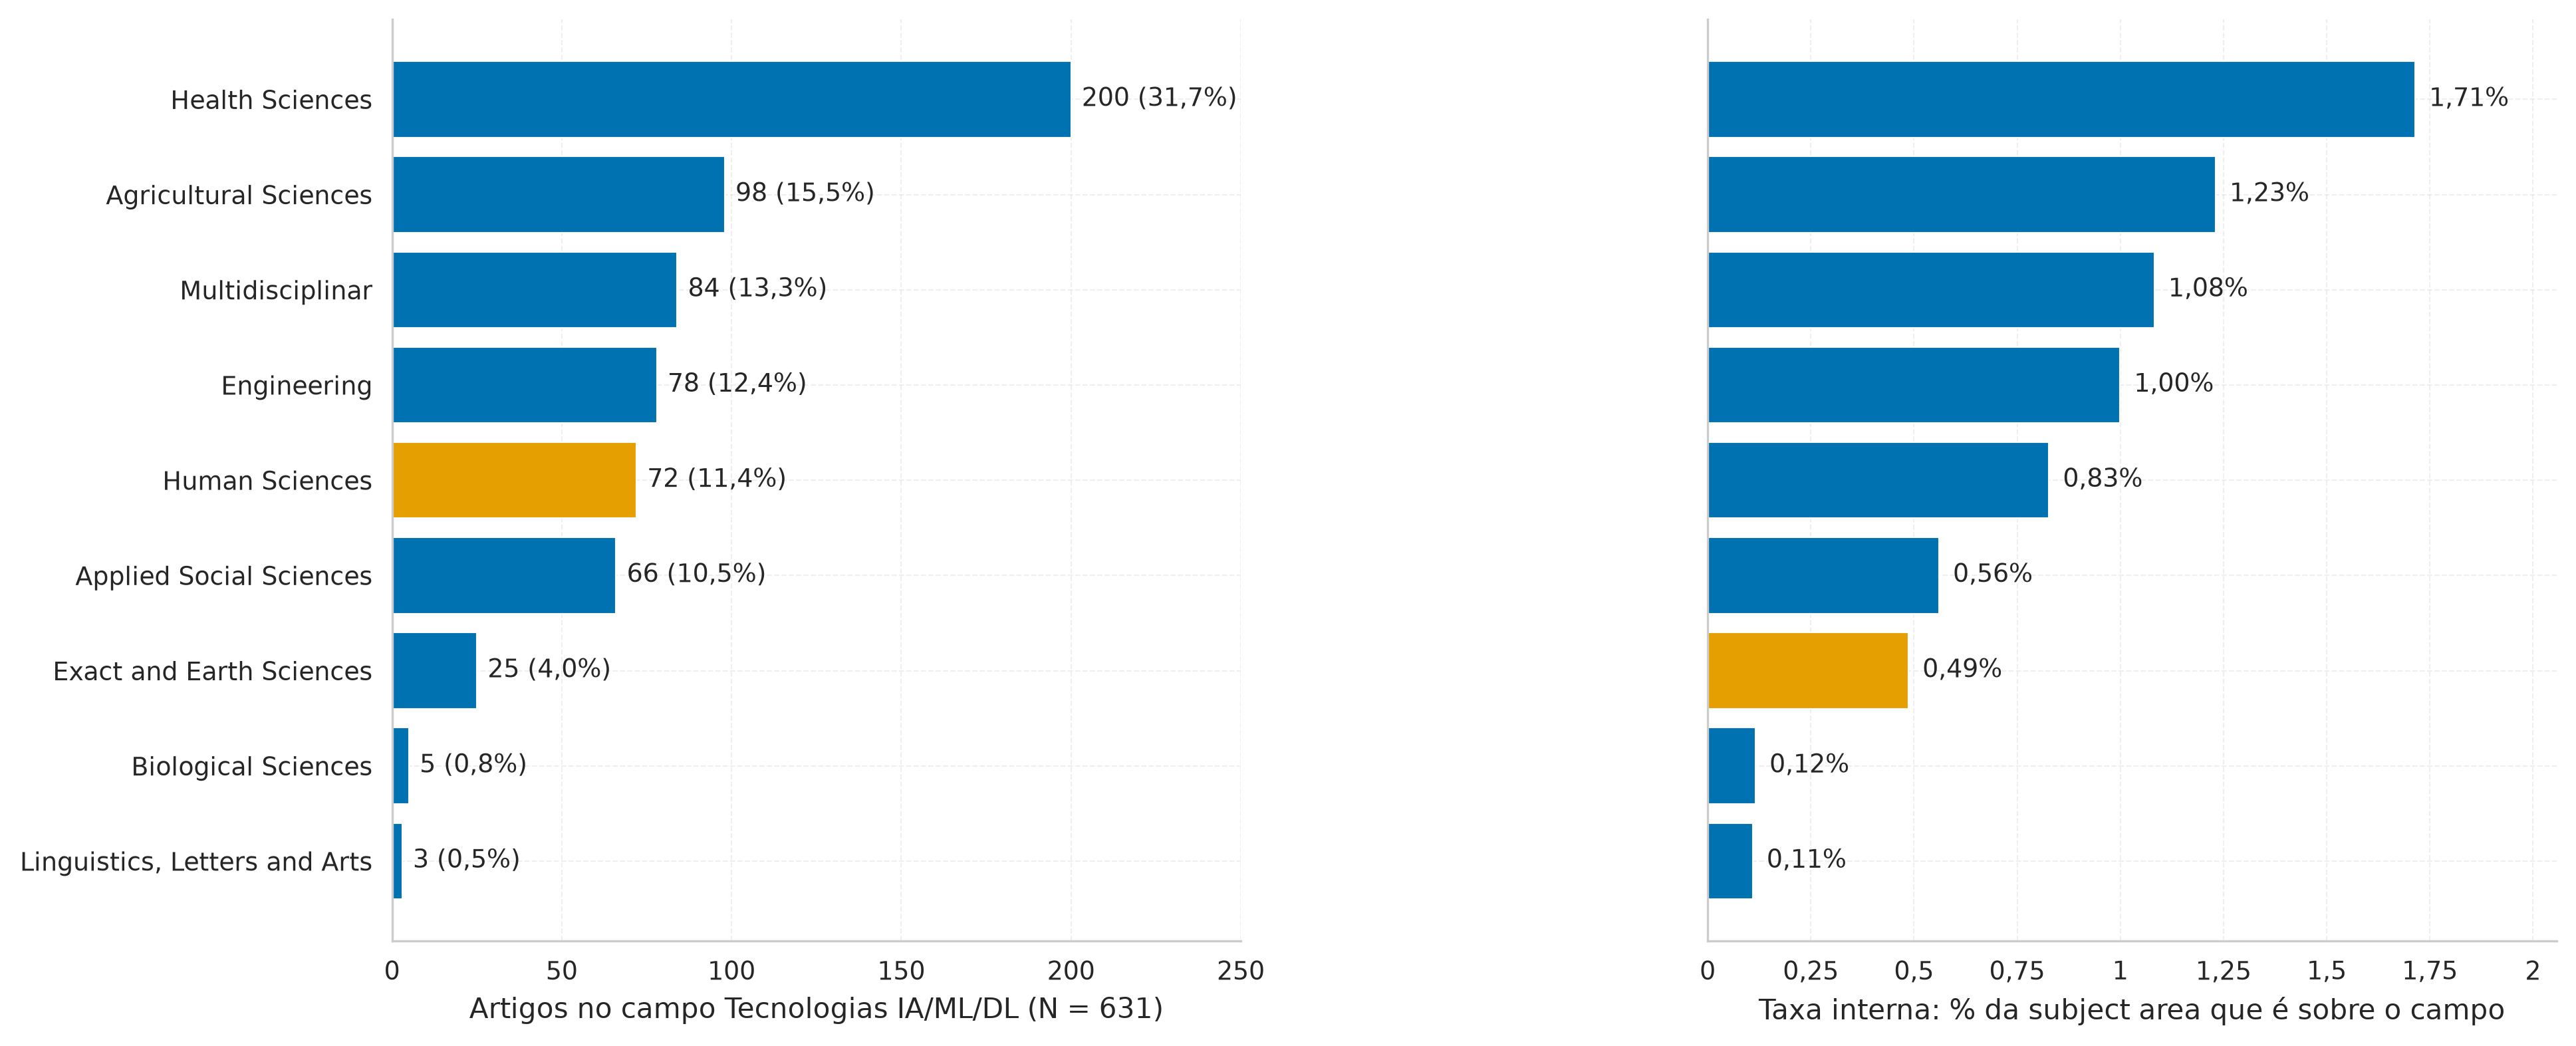
\includegraphics[width=0.95\linewidth]{figuras/cap.2/capes-scielo/scielo_11_subject_area_share.png}
    \caption[Distribuição do corpus \texttt{SciELO} por subject\_area, 2021--2024]{%
        Distribuição dos 631 artigos sobre inteligência artificial, aprendizado de máquina e aprendizado profundo publicados na coleção brasileira do \texttt{SciELO} no quadriênio 2021--2024, pela \emph{subject\_area} primária do periódico. O painel da esquerda mostra o volume absoluto e a participação no corpus, e o painel da direita mostra a taxa interna, isto é, a fração dos artigos de cada área que tocam o campo. As Ciências da Saúde lideram em volume, com 200 artigos, e as Engenharias registram a maior taxa interna, com 1,71\%. As Ciências Humanas, em destaque, respondem por 72 artigos e taxa interna de 0,49\%, magnitude próxima da que a \texttt{Capes} Humanas registra, com 0,67\%. A categoria Multidisciplinar reúne os periódicos cuja classificação no \texttt{SciELO} lista mais de uma área. Elaboração própria a partir da \emph{API} ArticleMeta da coleção brasileira do \texttt{SciELO}. Dados, \emph{scripts} e figuras versionados em \protect\url{https://github.com/julianehelanski/bibliometria-ia-humanas}.}
    \label{fig:scielo_subject_area}
\end{figure}

A interpretação da Figura~\ref{fig:scielo_subject_area} fortalece a primeira camada do achado. As Ciências Humanas, no \texttt{SciELO}, aparecem com 72 artigos e taxa interna de 0,49\%, valor próximo dos 0,67\% que a \texttt{Capes} Humanas registra na produção de pós-graduação. As duas bases foram construídas por plataformas e procedimentos distintos, e descrevem objetos distintos, a tese e o artigo, e ainda assim devolvem a mesma ordem de grandeza para a presença das Ciências Humanas no campo da inteligência artificial. A marginalidade que descrevi pela \texttt{Capes} reaparece quando a base muda da tese e da dissertação para o artigo publicado em periódico, e a convergência entre as duas análises paralelas sustenta a leitura de que essa marginalidade não é efeito do tipo de documento que uma das bases indexa.

Ao distribuir os 631 artigos pelos cinco subcampos do classificador, leio uma segunda diferença entre as duas bases, que disponho na Figura~\ref{fig:scielo_subcampos}. No \texttt{SciELO}, o subcampo mais frequente é a inteligência artificial em sentido estrito, com 187 artigos, ao passo que na \texttt{Capes} esse mesmo subcampo aparece só em quarto lugar, atrás do aprendizado de máquina, que lidera a pós-graduação com 5.284 trabalhos. A hierarquia, em suma, inverte: o que predomina no artigo de periódico é justamente o que rareia na tese. Leio essa inversão como efeito dos dois tipos de escrita que as duas bases capturam, pois o periódico publica a inteligência artificial sobretudo como conceito a discutir, e a pós-graduação a pesquisa sobretudo como técnica a aplicar. Cada veículo privilegia um recorte distinto do campo, e só a leitura das duas bases em paralelo faz com que essa diferença apareça.

\begin{figure}[htbp]
    \centering
    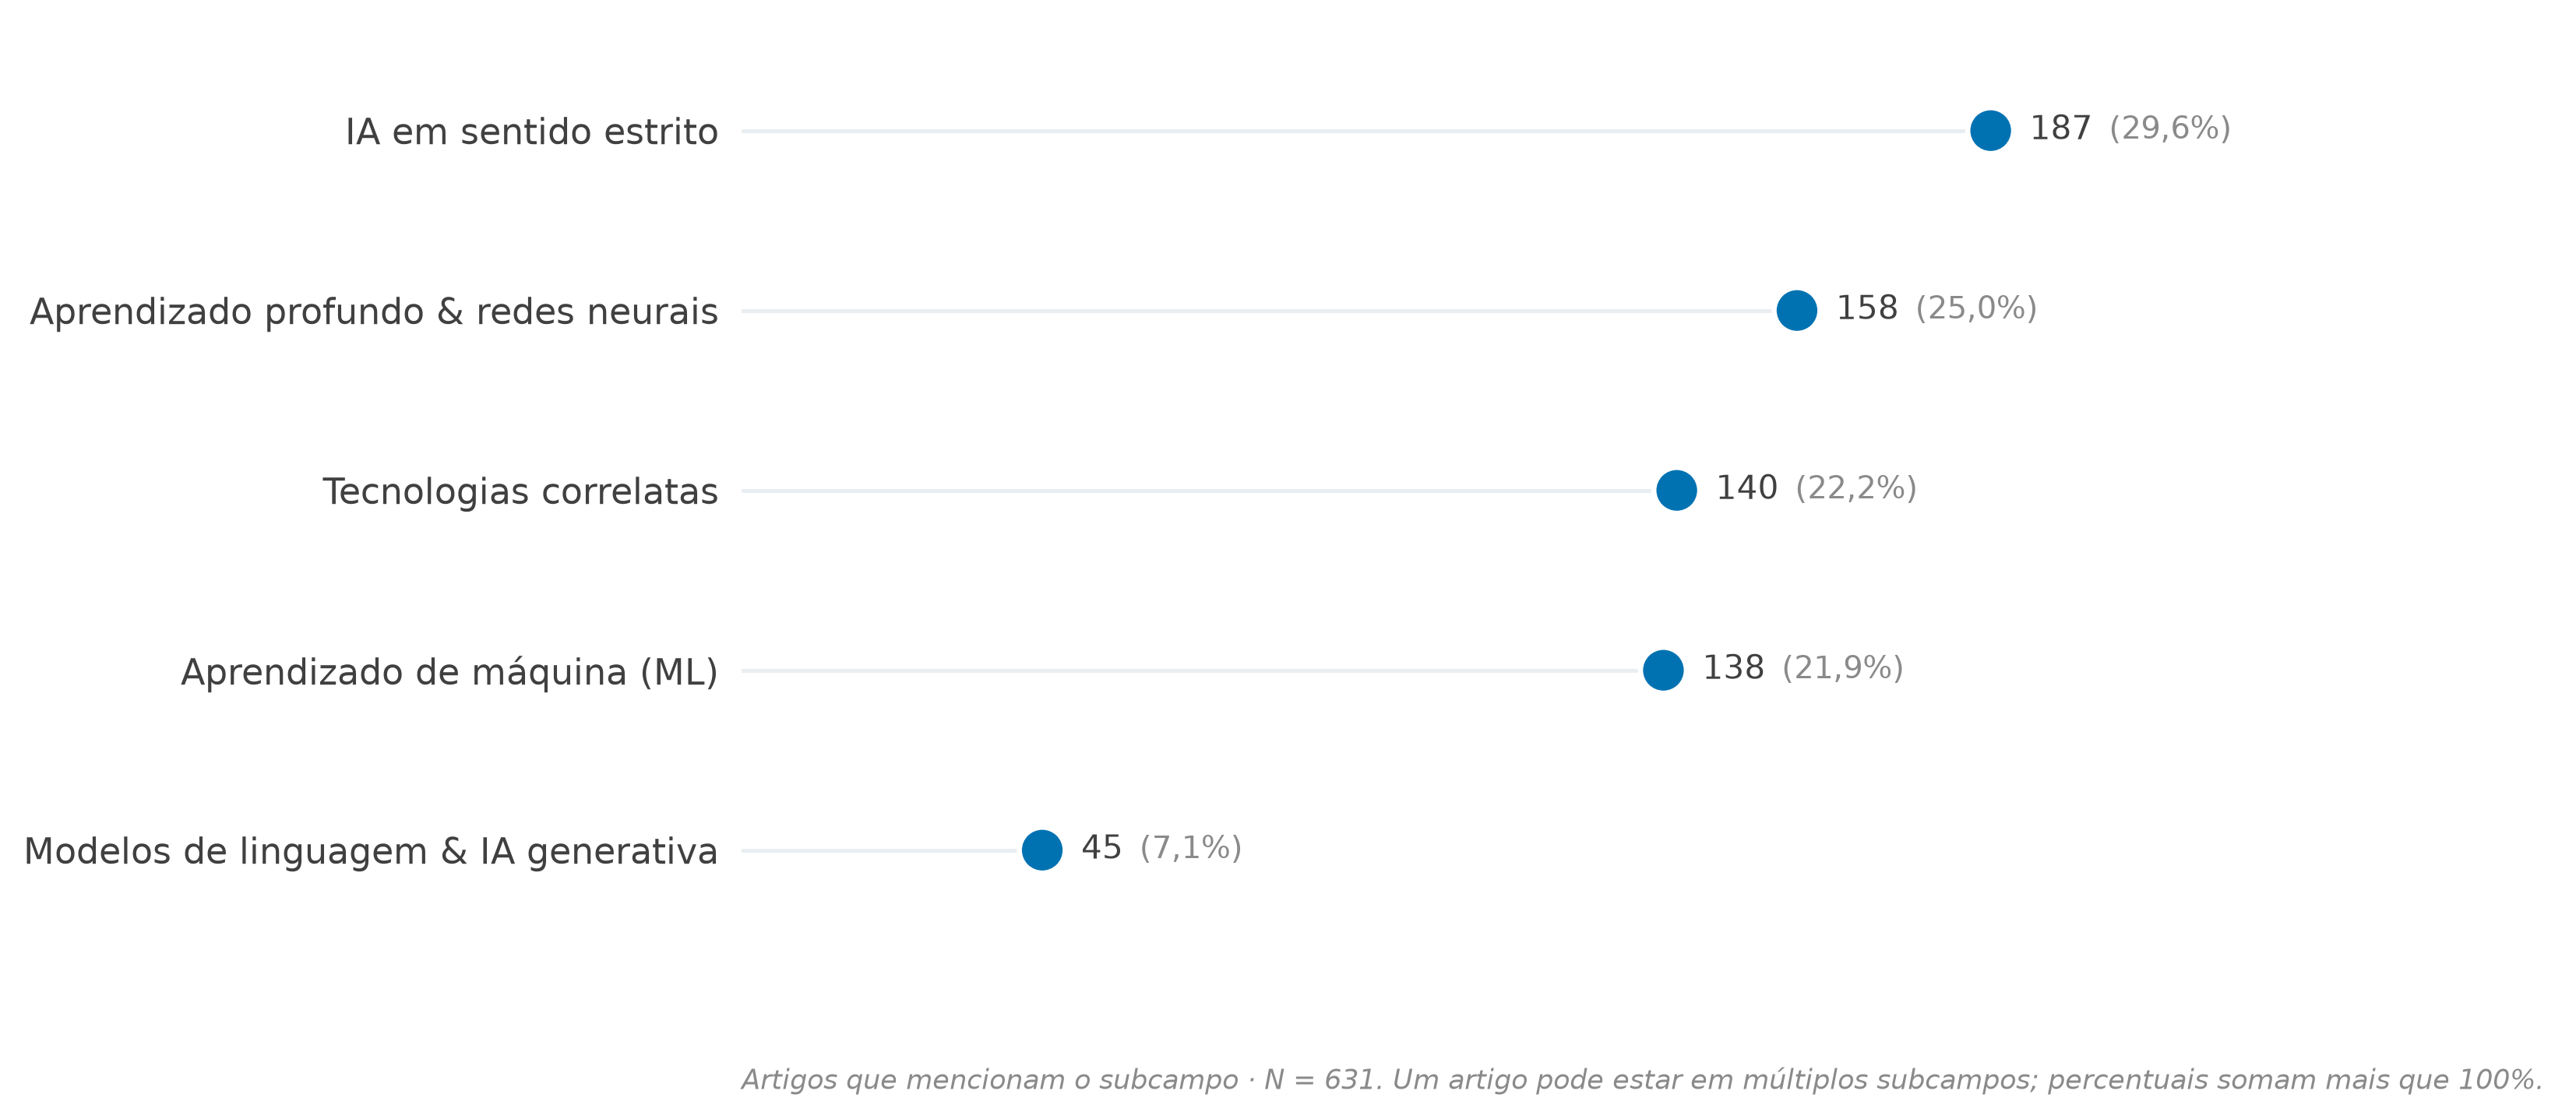
\includegraphics[width=0.85\linewidth]{figuras/cap.2/capes-scielo/scielo_21_subcampos_distribuicao.png}
    \caption[Distribuição do corpus \texttt{SciELO} por subcampo, 2021--2024]{%
        Distribuição dos 631 artigos do corpus \texttt{SciELO} pelos cinco
        subcampos do classificador. Um mesmo artigo pode pertencer a mais de um subcampo, e por isso a soma dos percentuais ultrapassa cem. A inteligência artificial em sentido estrito é o subcampo mais frequente, com 187 artigos, e o aprendizado de máquina aparece em quarto lugar, com 138, atrás das tecnologias correlatas, com 140, hierarquia que inverte a do Catálogo da \texttt{Capes}, em que o aprendizado de máquina lidera. A inversão sustenta a leitura de que o
        periódico publica a inteligência artificial como conceito e a
        pós-graduação a pesquisa como técnica aplicada. Elaboração própria a
        partir da \emph{API} ArticleMeta da coleção brasileira do \texttt{SciELO}. Dados, \emph{scripts} e figuras versionados em \protect\url{https://github.com/julianehelanski/bibliometria-ia-humanas}.}
    \label{fig:scielo_subcampos}
\end{figure}

O \texttt{SciELO} acrescenta um ponto relevante sobre essas publicações, referente aos tipos de veículos que a Antropologia brasileira utiliza para publicar pesquisas sobre inteligência artificial.\footnote{O recorte de Ciências Humanas que comparo com a \texttt{Capes} é o subset das Ciências Humanas em sentido estrito, isto é, os 72 artigos publicados em periódicos cuja \emph{subject\_area} é exatamente \enquote{Human Sciences}, sem a categoria Multidisciplinar. Esse recorte estrito é o que estabelece a paridade com a grande área Ciências Humanas do Catálogo da \texttt{Capes}, e dele que saem os números de periódicos discutidos neste parágrafo.} No subset das Ciências Humanas em sentido estrito, a revista \textit{Mana}, periódico de referência da Antropologia brasileira, aparece com três artigos. Os três foram publicados em 2024, e os três tocam o campo pela porta do \emph{big data}, e não da inteligência artificial em sentido estrito. A Antropologia, quando entra na conversa em seu próprio periódico de referência, entra tarde, em 2024, e por um vocabulário deslocado em relação ao objeto. O achado do \texttt{SciELO} compõe com o da \texttt{Capes} uma leitura em duas camadas: a \texttt{Capes} mostra a escassez da tese e da dissertação de Antropologia sobre inteligência artificial, e o \texttt{SciELO} mostra que, quando a disciplina publica o artigo, publica-o pelo tema \emph{big data}. As duas bases, cada uma com seu objeto, sustentam o mesmo diagnóstico de uma emergência tardia e tematicamente deslocada.

O mapeamento que fiz nesta seção mostra que as duas bases estão alinhadas em seus principais achados. O primeiro é que o acesso ampliado à inteligência artificial generativa, a partir do final de 2022, produziu uma aceleração visível nas duas ao mesmo tempo, na produção de pós-graduação que a \texttt{Capes} reúne e na produção de periódico que a \texttt{SciELO} reúne. O segundo é que a presença da inteligência artificial nas ciências humanas, além de pequena, distribui-se de modo desigual por dentro. As duas bases chegam à mesma ordem de grandeza para o conjunto das Ciências Humanas por caminhos separados, 0,67\% das defesas na \texttt{Capes} e 0,49\% dos artigos na \texttt{SciELO}, duas medidas próximas obtidas sobre objetos distintos, a tese e o artigo, e a proximidade entre elas me autoriza a ler esses números como característica do próprio campo, e não como efeito do documento que cada base indexa. Dentro desse conjunto já reduzido, a distribuição é ainda maior: a Educação concentra 38,5\% das defesas, ao passo que a Antropologia, com quatro defesas e 1,0\%, aparece quase no fim, à frente apenas da Arqueologia.

A dispersão temática que encontro nas duas bases, da automação industrial à arte contemporânea, do policiamento preditivo às estatísticas oficiais, da saúde da mulher ao \emph{big data} eleitoral, suscita algumas questões que deixo em aberto. Será que o campo está disperso porque o objeto é, ele próprio, heterogêneo? A inteligência artificial abrange várias técnicas, infraestruturas e relações que se ramificam por toda parte. Pode ser que esteja disperso porque as ciências humanas brasileiras são plurais por constituição, e cada disciplina encontra a inteligência artificial pela vizinhança dos seus próprios objetos. Pode ser, ainda, que o campo seja novo demais para ter convergido, e que a dispersão de hoje seja a forma provisória de um campo em formação. Ou pode ser que essa dispersão não seja transitória nem acidental, e sim o indício de algo mais estrutural, a saber, que a inteligência artificial já está tão entranhada no trabalho, na política, na saúde e na cultura que pesquisá-la em separado, como objeto autônomo, talvez seja a abordagem menos provável justamente porque ela está em toda parte. Inclino-me para essa última leitura, sem descartar as outras, e deixo a tensão entre elas como uma das perguntas que estudos futuros poderão investigar com mais profundidade.

A Figura~\ref{fig:comparativo_scielo_capes} reúne essa leitura paralela das duas bases brasileiras em quatro painéis, com o mesmo classificador de cinco subcampos aplicado às duas e com recorte de escopo equivalente, a \texttt{SciELO} restrita ao subset de Ciências Humanas em sentido estrito e a \texttt{Capes} restrita à grande área Ciências Humanas. Os dois painéis superiores cruzam a evolução temporal e a distribuição por subcampo, e as duas bases crescem em ritmo próximo, 112\% na \texttt{SciELO} e 106\% na \texttt{Capes} entre 2021 e 2024, e cada uma pende para um lado, o periódico para a inteligência artificial como conceito e a tese para a técnica aplicada. Os dois painéis inferiores descem ao detalhe de cada base, os periódicos de Ciências Humanas em que a \texttt{SciELO} concentra os artigos e as áreas de conhecimento em que a \texttt{Capes} concentra as defesas, e situam, nos dois recortes, a posição marginal da Antropologia: cada base alcança um aspecto que a outra não vê, pois a \texttt{Capes} reúne programas e dá a leitura caso a caso das quatro defesas, e o \texttt{SciELO} reúne periódicos e dá os três artigos da revista \textit{Mana}, e os dois recortes fecham a mesma figura de uma disciplina que entra no campo por último e por uma porta lateral.

\begin{figure}[htbp]
    \centering
    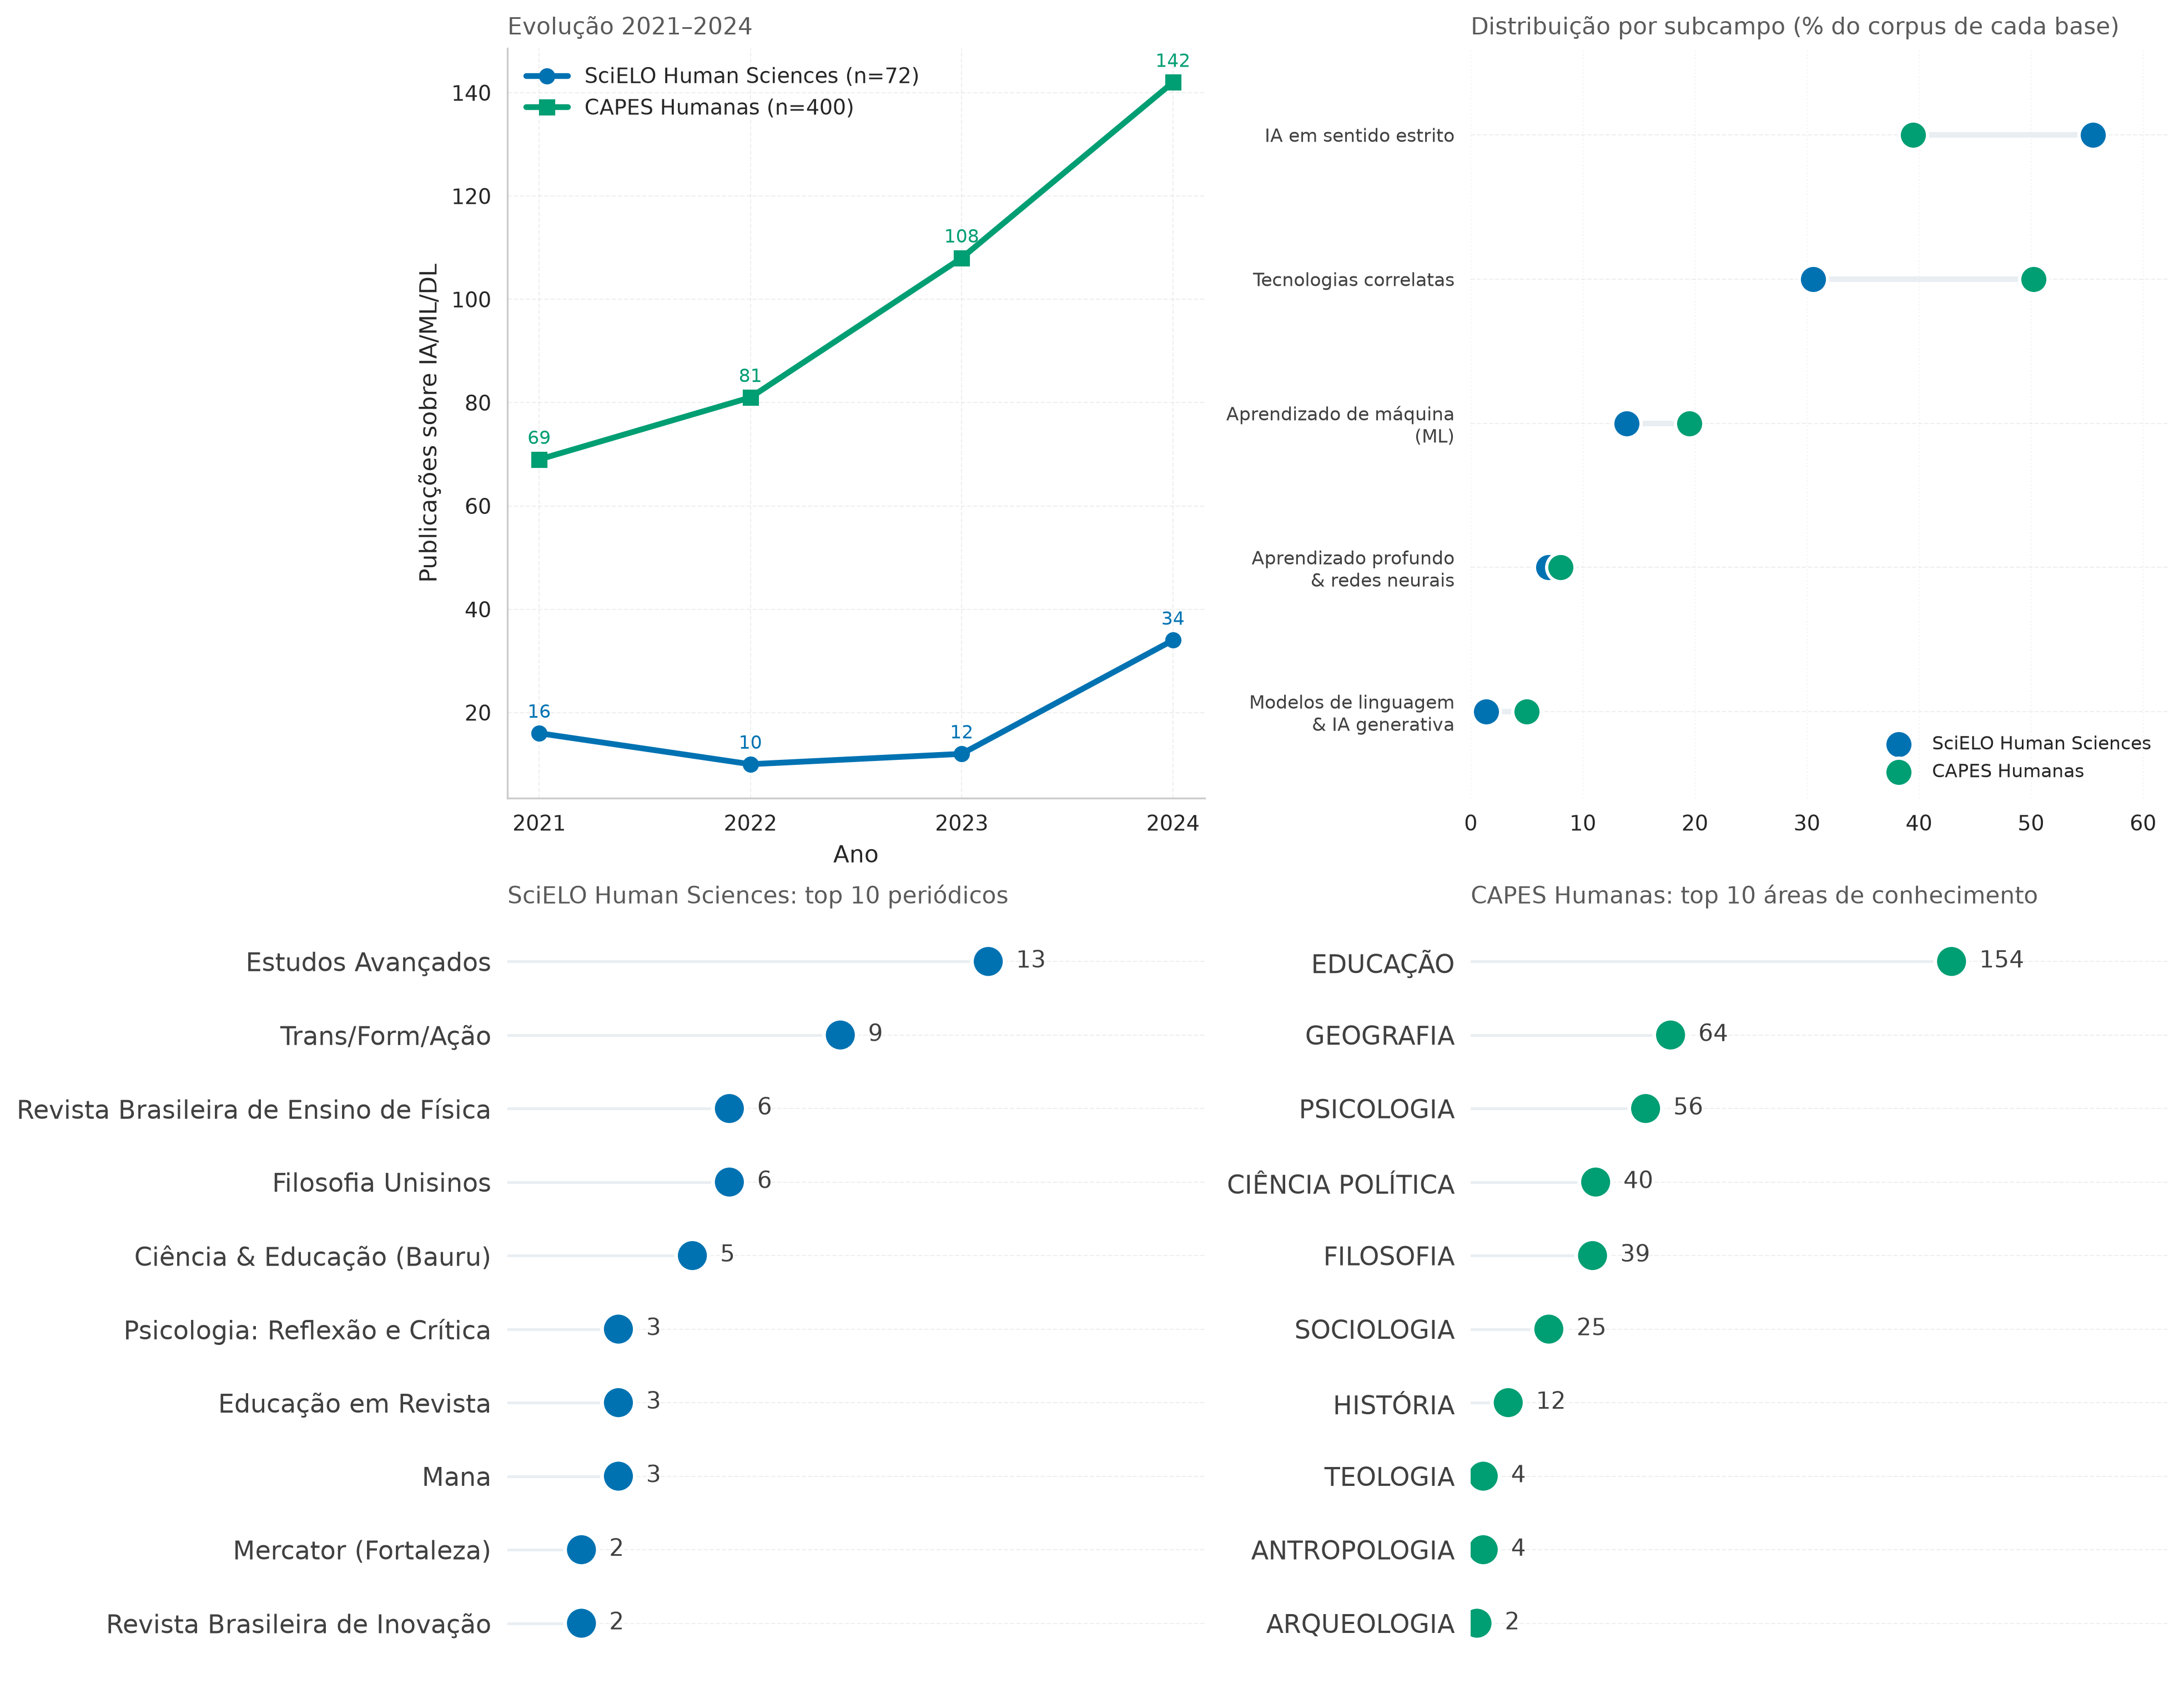
\includegraphics[width=1.0\linewidth]{figuras/cap.2/capes-scielo/comparativo_scielo_capes_2026.png}
    \caption[Análise comparativa \texttt{SciELO} e \texttt{Capes} nas Ciências Humanas, 2021--2024]{%
        Leitura paralela das duas bases sobre o quadriênio 2021--2024, com o
        mesmo classificador de cinco subcampos aplicado a cada uma e recorte de
        escopo equivalente: o \texttt{SciELO} restrito ao subset de Ciências
        Humanas em sentido estrito, sem a categoria Multidisciplinar, e a
        \texttt{Capes} restrita à grande área Ciências Humanas. O painel A
        sobrepõe a evolução temporal: o \texttt{SciELO} de Ciências Humanas
        cresce de 16 para 34 artigos sobre o campo, e a \texttt{Capes} Humanas
        cresce de 69 para 142 defesas. O painel B põe lado a lado a distribuição
        por subcampo, com o \texttt{SciELO} mais inclinado à inteligência
        artificial como conceito e a \texttt{Capes} mais inclinada às
        tecnologias correlatas, sobretudo pelo caminho da Educação. O painel C traz
        os dez periódicos do \texttt{SciELO} de Ciências Humanas com mais
        artigos no campo, com \textit{Estudos Avançados} à frente, com 13, e a
        revista de Antropologia \textit{Mana} com 3. O painel D traz as dez
        áreas de conhecimento das defesas da \texttt{Capes} Humanas, com a
        Educação à frente, com 154, e a Antropologia com 4. Elaboração própria
        a partir da \emph{API} ArticleMeta da coleção brasileira do
        \texttt{SciELO} e do Catálogo de Teses e Dissertações da \texttt{Capes},
        \emph{dump} oficial \texttt{BR-CAPES-BTD-2021A2024}. Dados, \emph{scripts} e figuras versionados em \protect\url{https://github.com/julianehelanski/bibliometria-ia-humanas}.}
    \label{fig:comparativo_scielo_capes}
\end{figure}

A posição da antropologia dentro das ciências humanas se inscreve, por sua vez, na posição do Brasil no mapa mundial da inteligência artificial, como uma \enquote{semiperiferia} em movimento. Pelo levantamento do \texttt{CSET} (\emph{Center for Security and Emerging Technology}), que reúne artigos, trabalhos de conferência e \emph{preprints} sobre inteligência artificial em todas as áreas do conhecimento, o Brasil ocupou em 2024 a vigésima terceira posição mundial, com pouco mais de três mil publicações, e liderou com folga a América Latina \parencite{OWID2024AI}. Esta não é uma posição de quem está fora do mapa. O que me chama a atenção é o movimento da produção brasileira, que cresceu em números absolutos ao longo da década, e ainda assim recuou da décima terceira posição que ocupava em 2016 para a vigésima terceira em 2024, porque a aceleração de outros países foi mais rápida que a sua. O mesmo movimento aparece no mapeamento dos centros de inteligência artificial da \texttt{FAPESP}, que registra um Brasil entre os vinte maiores produtores em volume e, ao mesmo tempo, distante da fronteira de ponta, com presença discreta nas conferências de referência e produção concentrada em poucas instituições, com a \texttt{USP} à frente \parencite{Brandao2024Desenvolvimento}. É essa concentração que a própria política de criação dos centros, entre eles o \texttt{C4AI} de que trato no capítulo~\ref{capitulo3}, procura corrigir. As ciências humanas e sociais se aproximam da inteligência artificial a partir desse contexto geral de produção tecnocientífica de peso intermediário em escala mundial, de grande relevância na região e em relativo recuo, longe da periferia e longe do atraso.

O levantamento do \texttt{CSET} mede a inteligência artificial sem recorte de disciplina, e por isso não me diz onde, dentro da produção de cada país, a inteligência artificial entra. Para descer ao recorte que interessa à minha pesquisa, a inteligência artificial dentro das ciências humanas, recorri a uma terceira base, o \texttt{OpenAlex}, catálogo aberto de cerca de duzentos e cinquenta milhões de obras acadêmicas de todo o mundo.\footnote{O \texttt{OpenAlex} é um catálogo bibliográfico aberto, mantido pela organização \texttt{OurResearch} desde 2022 como sucessor do \texttt{Microsoft Academic Graph}, e indexa obras, autorias, instituições e os conceitos a elas atribuídos por classificação automática. Coletei o corpus com o \texttt{claude code} no terminal, em sessões iteradas de requisição à \emph{API} \emph{REST} da plataforma, classificação e auditoria, e apliquei a ele a mesma régua de cinco subcampos que apliquei ao Catálogo da \texttt{Capes} e à \texttt{SciELO}, de modo que os subcampos ficam comparáveis entre as três bases. Os números canônicos do recorte do \texttt{OpenAlex}, e a proveniência de cada figura, ficam versionados no arquivo \texttt{docs/decisoes\_metodologicas.md} do repositório.} O que faltava à \texttt{Capes} e à \texttt{SciELO}, e que o \texttt{OpenAlex} me dá, é a comparação por país e por disciplina ao mesmo tempo, isto é, a possibilidade de cruzar o conceito de inteligência artificial com a classificação das obras por \emph{field}, o campo do conhecimento que a taxonomia da plataforma herda da base \texttt{Scopus}.\footnote{O \emph{field} é a unidade intermediária da taxonomia do \texttt{OpenAlex}, importada da classificação \emph{ASJC} (\emph{All Science Journal Classification}) da \texttt{Scopus}, comunidade da bibliometria internacional. Para espelhar a grande área Ciências Humanas do Catálogo da \texttt{Capes}, que abriga também a Psicologia, adotei o recorte amplo que reúne três \emph{fields}, o de Artes e Humanidades, o de Psicologia e o de Ciências Sociais. A escolha do recorte é uma decisão metodológica, e não um dado, e por isso a declaro: outra pesquisadora que adotasse só o \emph{field} de Artes e Humanidades, ou que somasse outros \emph{fields}, encontraria magnitudes distintas. Os identificadores dos três \emph{fields} foram conferidos diretamente na \emph{API} em seu estado de seis de junho de 2026, porque a taxonomia da plataforma evolui no tempo. A janela é 2016--2024, alinhada à do \texttt{CSET}.}

Antes de partir aos números do \texttt{OpenAlex}, preciso enfrentar uma divergência que a base devolve sobre si mesma, e que toca o problema que percorre esta seção inteira, o de saber o que conta como inteligência artificial. A mesma base, sobre o mesmo recorte brasileiro de humanidades, produz dois números muito distantes conforme o critério que escolho para dizer que uma obra é de inteligência artificial. Pelo conceito que o próprio \texttt{OpenAlex} atribui às obras por classificação automática, o Brasil registra 9.996 obras de inteligência artificial nas humanidades no período; pela régua de palavra-chave, a mesma que sustenta os números da \texttt{Capes} e da \texttt{SciELO}, apenas 849 obras únicas trazem, de fato, vocabulário de inteligência artificial no título ou no resumo. Somente cerca de 8,5\% das obras que o classificador do \texttt{OpenAlex} marca como inteligência artificial contêm esse vocabulário explícito, e leio esse abismo de duas maneiras que se somam: o conceito atribuído pela máquina é generoso e alcança obras que apenas tangenciam o campo, e parte das obras indexadas não traz resumo, o que deixa a régua de palavra-chave com menos texto para cruzar.\footnote{O conceito \enquote{\emph{Artificial intelligence}} do \texttt{OpenAlex} é atribuído por um modelo de classificação que lê os metadados de cada obra e lhe associa conceitos com um grau de confiança, e por isso alcança obras cuja relação com o campo é de vizinhança temática, e não de objeto. A régua de palavra-chave, ao contrário, exige a presença de um termo do campo no título ou no resumo, e é, das duas, a mais próxima do gesto que faço nas outras bases. O número comparável à \texttt{Capes} e à \texttt{SciELO} é o das 849 obras únicas, e não o das 9.996. A contagem por obra única deduplica a contagem por afiliação, em que uma obra é somada uma vez para cada país de seus autores, e que para o Brasil chegava a 15.438 registros, inflada pela coautoria internacional.} Esse desencontro entre os dois critérios me mostra que medir a presença da inteligência artificial exige, antes de tudo, uma decisão sobre o que se está disposto a chamar de inteligência artificial, e a distância entre 9.996 e 849 é a distância entre um campo tomado por vizinhança conceitual e um campo tomado por nomeação explícita. Por isso a comparação internacional de volume e de penetração, mais uniforme entre países, segue o conceito da plataforma, e a análise de subcampos, que precisa falar a mesma língua das outras duas bases, segue a régua de palavra-chave.

\begin{figure}[htbp]
    \centering
    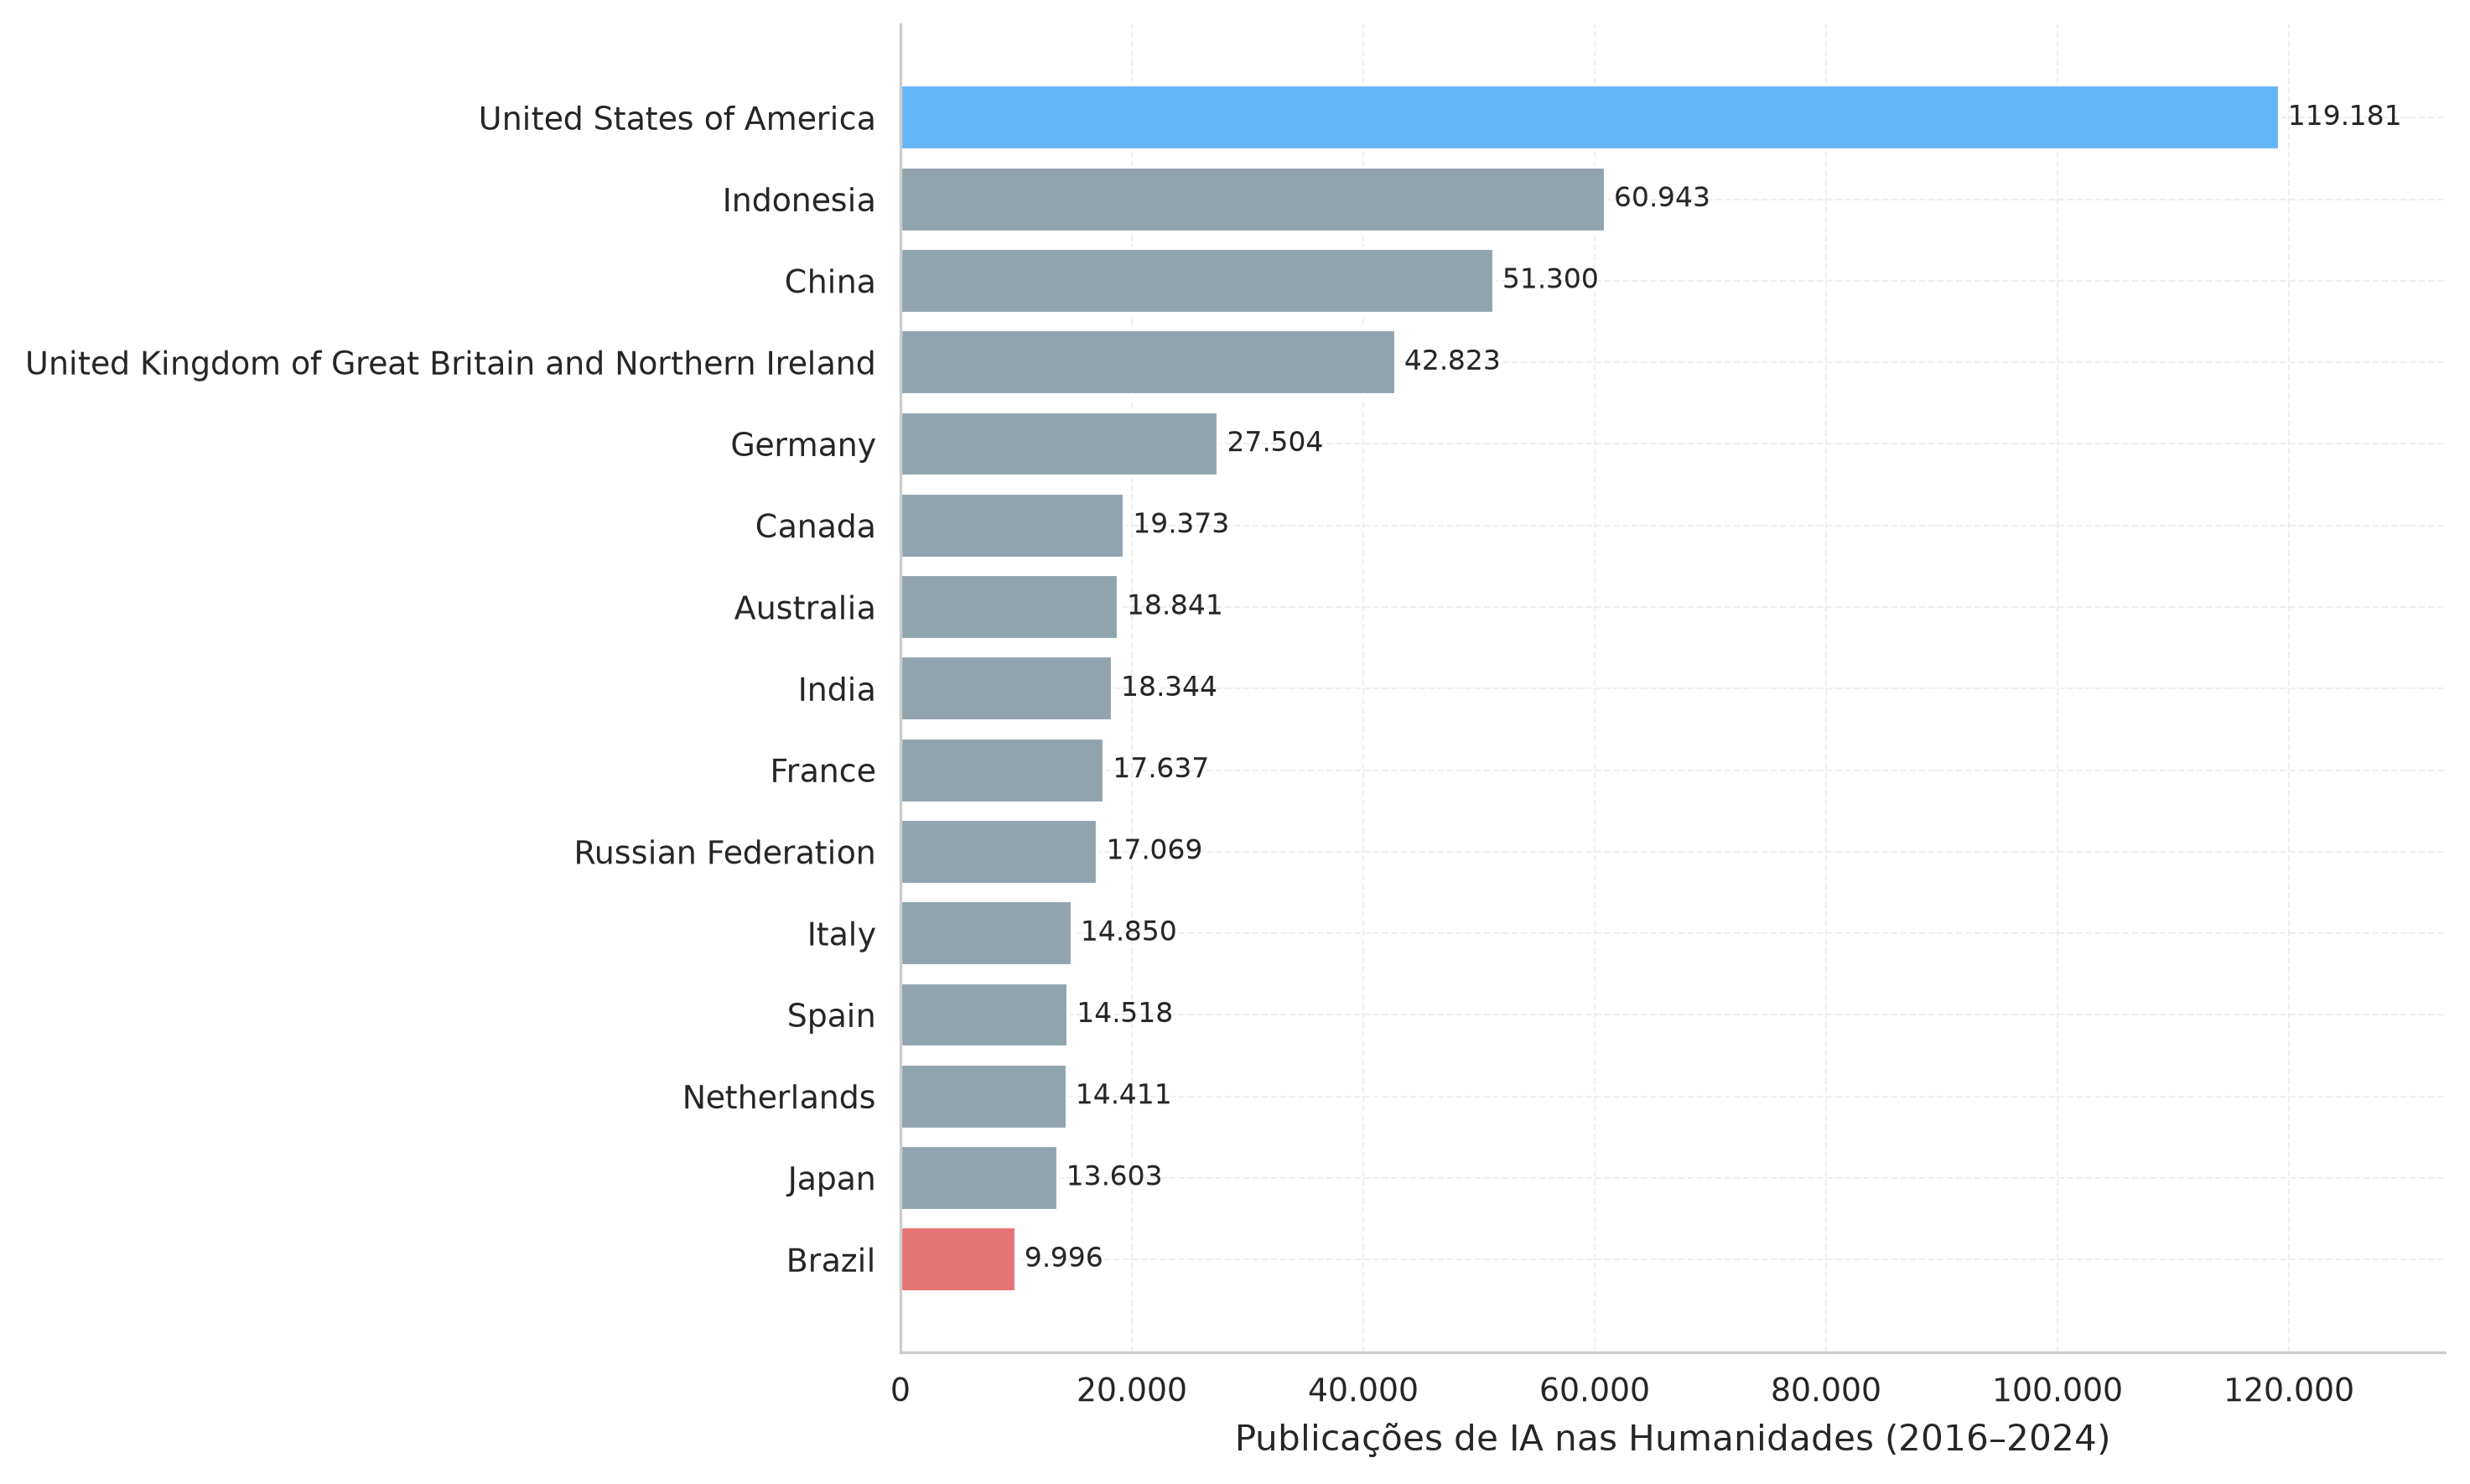
\includegraphics[width=0.85\linewidth]{figuras/cap.2/openalex_01_ranking_paises.png}
    \caption[Maiores produtores de IA nas Humanidades, \texttt{OpenAlex} 2016--2024]{%
        Os quinze maiores produtores de obras sobre inteligência artificial na
        grande área de Humanidades no período 2016--2024, pela definição por
        conceito do \texttt{OpenAlex}, em volume absoluto. O Brasil, em destaque,
        ocupa a décima quinta posição mundial, com 9.996 obras, atrás de
        produtores como os Estados Unidos, com cerca de 119 mil, a China, com
        51,3 mil, o Reino Unido, com 42,8 mil, e a Alemanha, com 27,5 mil. A
        Indonésia, em segundo lugar, e a Índia, em oitavo, sobem no volume
        porque têm universos de humanidades muito grandes, e essa presença
        antecipa por que a leitura por volume precisa ser corrigida pela taxa
        interna. Elaboração própria a partir do \texttt{OpenAlex}. Repositório
        com dados, \emph{scripts} e figuras em \protect\url{https://github.com/julianehelanski/bibliometria-ia-humanas}.}
    \label{fig:openalex_ranking_paises}
\end{figure}

A Figura~\ref{fig:openalex_ranking_paises} mostra uma concentração geográfica acentuada, com os Estados Unidos e a China à frente por larga distância, seguidos do Reino Unido e da Alemanha. Uma inversão me interessa de perto: nas estatísticas de inteligência artificial em todas as áreas, como as do \texttt{CSET} que citei acima, a China supera os Estados Unidos em volume, e quando o recorte se fecha sobre as humanidades os Estados Unidos retomam a dianteira. A interseção entre inteligência artificial e humanidades tem geografia própria, distinta da inteligência artificial tomada em sentido amplo, e por isso o ranking do \texttt{OpenAlex} que leio aqui não é o mesmo que o do \texttt{CSET} do parágrafo anterior, pois um mede o campo inteiro e o outro mede o recorte disciplinar. O Brasil, com 9.996 obras, figura em décimo quinto lugar, presença que não é desprezível em volume absoluto, e que, vista assim, repete a leitura de semiperiferia que o \texttt{CSET} já dava. O volume, porém, esconde o achado, e é a próxima figura que o revela.

\begin{figure}[htbp]
    \centering
    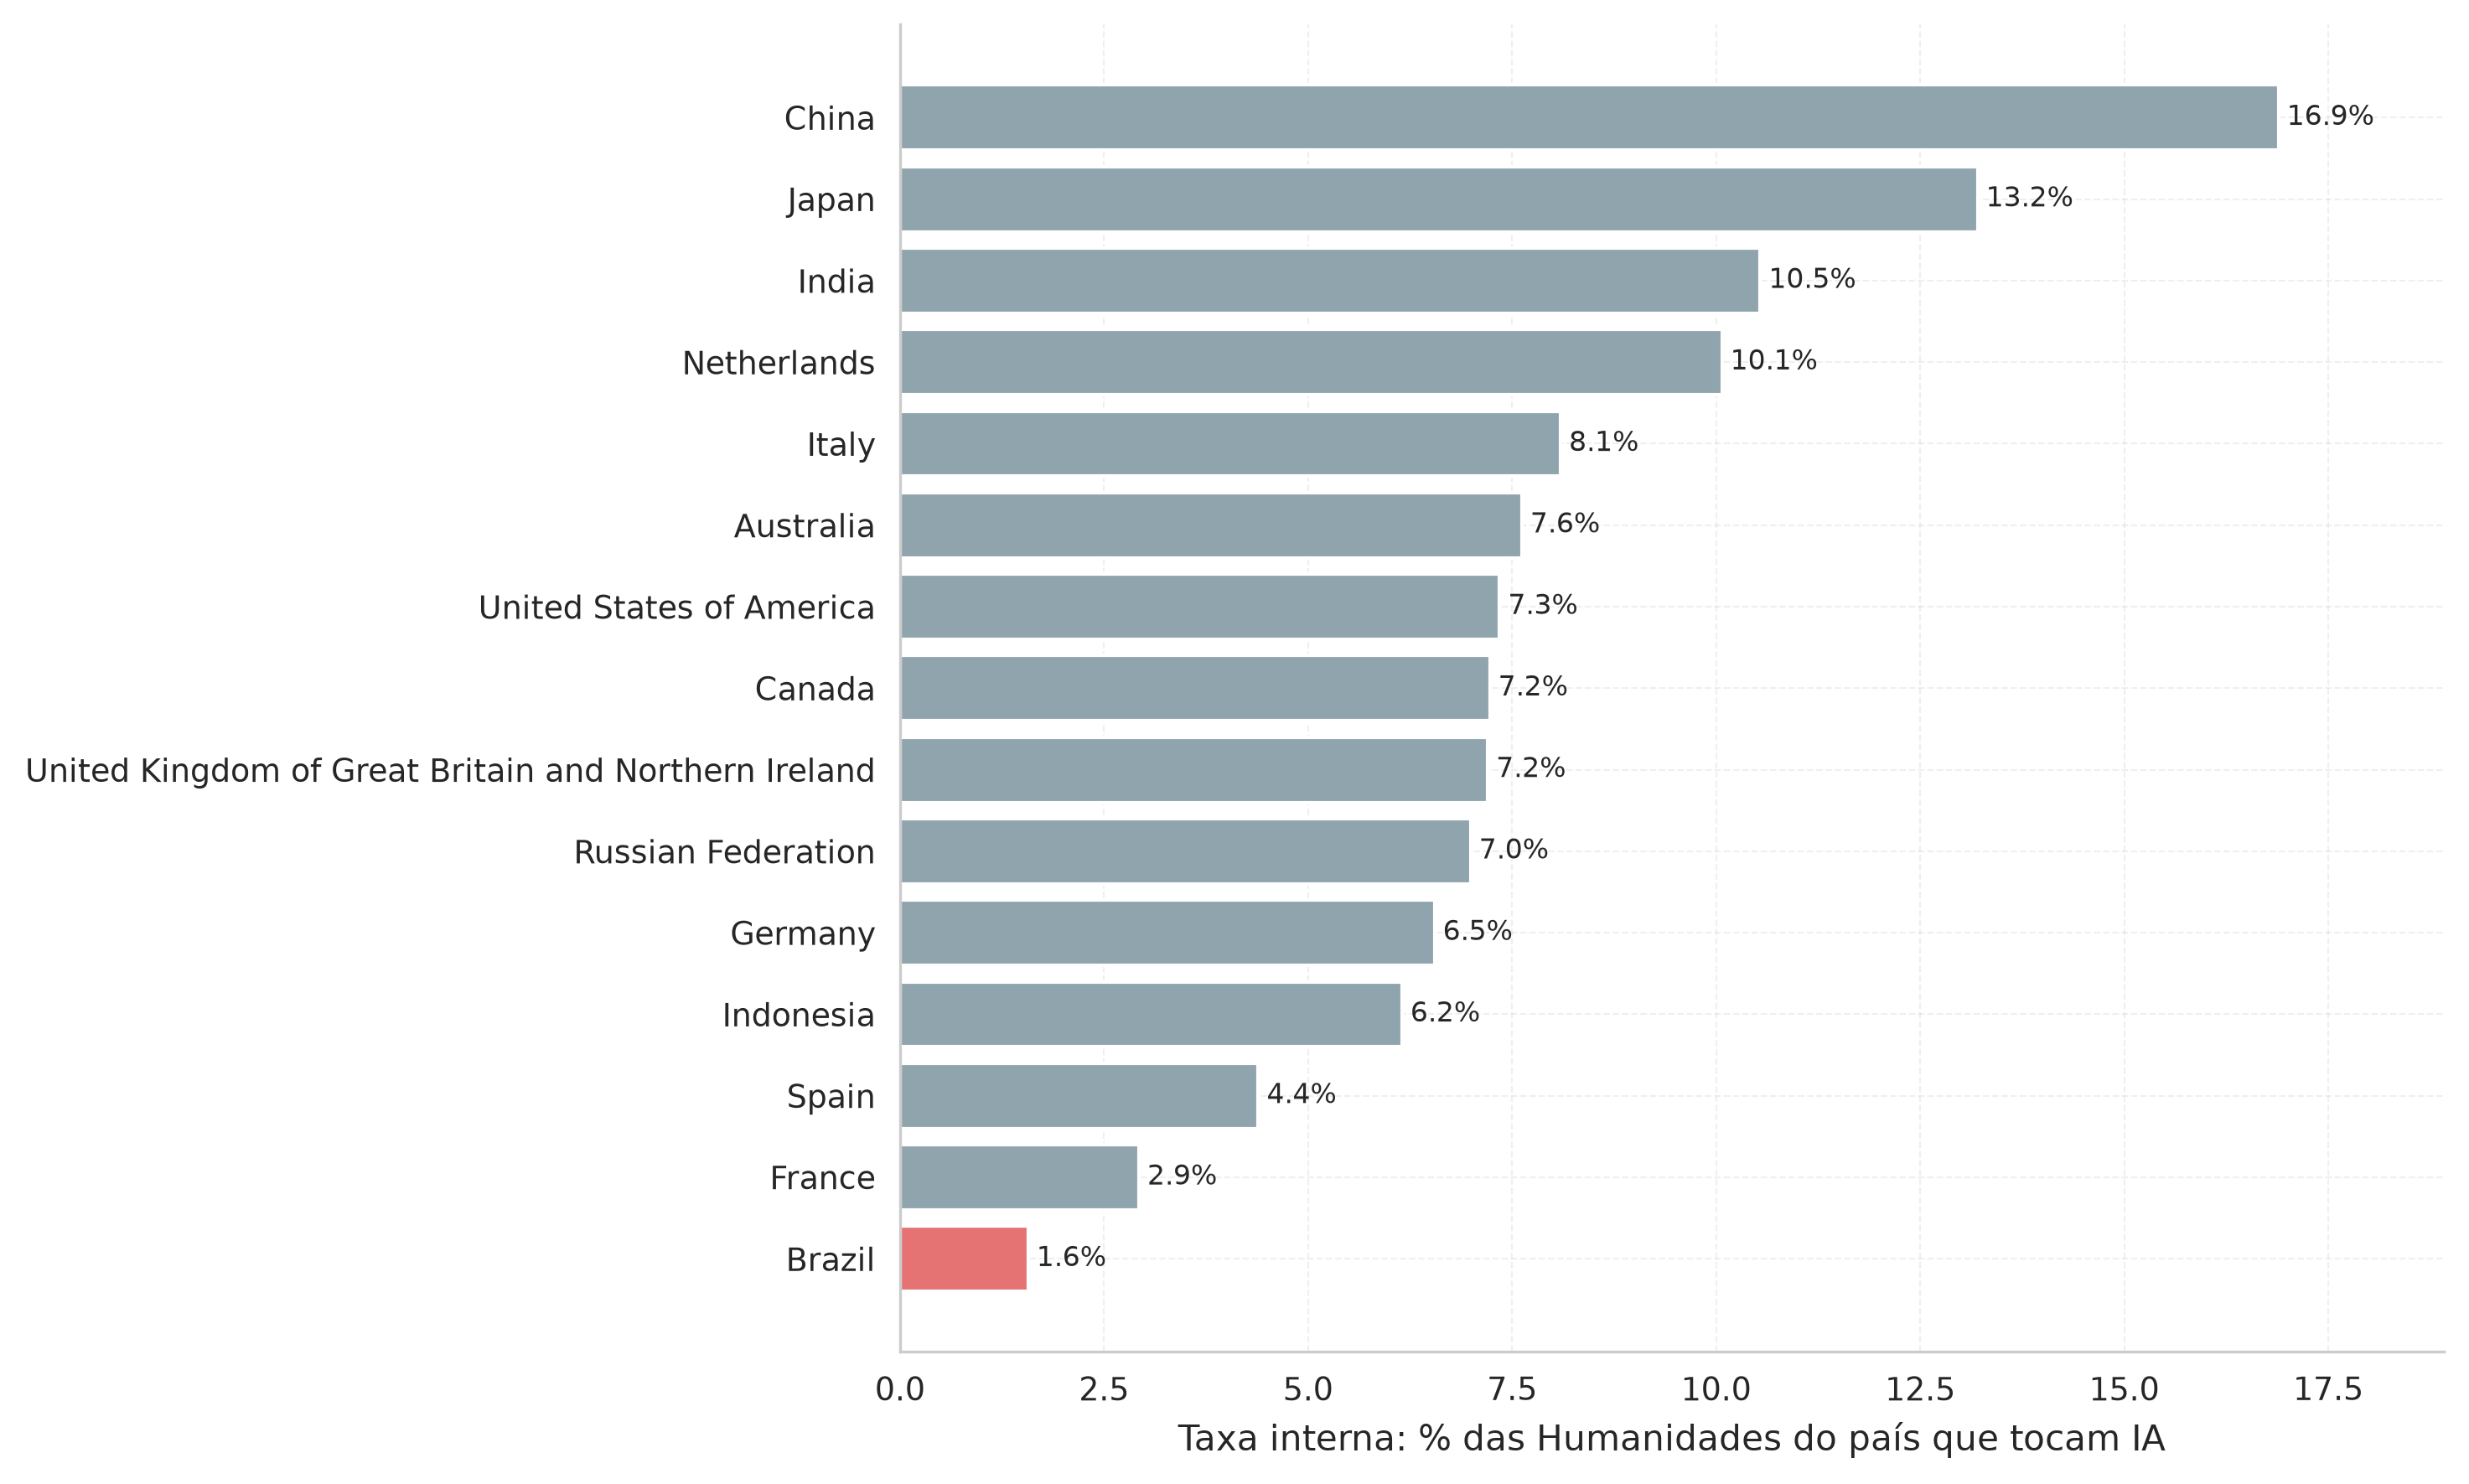
\includegraphics[width=0.85\linewidth]{figuras/cap.2/openalex_02_taxa_interna_paises.png}
    \caption[Taxa interna de IA nas Humanidades por país, \texttt{OpenAlex} 2016--2024]{%
        Taxa interna, isto é, a fração das obras de Humanidades de cada país que
        tocam o campo da inteligência artificial, entre os quinze maiores
        produtores em volume, no período 2016--2024, pela definição por
        conceito do \texttt{OpenAlex}. Apesar do volume que o coloca em décimo
        quinto lugar, o Brasil, em destaque, apresenta a menor taxa do grupo,
        com 1,57\%, contra 16,89\% da China, 13,20\% do Japão e 6,15\% dos
        Estados Unidos. O Brasil tem o segundo maior universo de Humanidades do
        conjunto, com 636.607 obras, atrás apenas dos Estados Unidos, e ainda
        assim é o que menos conecta essa produção à inteligência artificial.
        Elaboração própria a partir do \texttt{OpenAlex}. Repositório com dados,
        \emph{scripts} e figuras em \protect\url{https://github.com/julianehelanski/bibliometria-ia-humanas}.}
    \label{fig:openalex_taxa_interna}
\end{figure}

A leitura por taxa interna, a fração das humanidades de cada país que dialoga com a inteligência artificial, inverte o quadro que o volume sugere, e a Figura~\ref{fig:openalex_taxa_interna} a apresenta. A China lidera a penetração, com 16,89\%, seguida do Japão, com 13,20\%, da Índia, com 10,54\%, e dos Países Baixos, com 10,07\%, e os Estados Unidos, primeiros em volume, ficam em um patamar intermediário, com 6,15\%. O Brasil ocupa o último lugar entre os quinze maiores produtores, com apenas 1,57\%. O dado pesa mais quando observo que o Brasil tem o segundo maior universo de humanidades do conjunto, com 636.607 obras, atrás apenas dos Estados Unidos. O Brasil produz muito em humanidades, e dessa produção vasta pouco se volta para a inteligência artificial, e é esse contraste entre o tamanho do universo e a estreiteza da fração que define a posição brasileira. O achado replica, em escala internacional, a marginalidade que descrevi pela \texttt{Capes}, em que 0,67\% das defesas de Ciências Humanas tocam o campo, e pela \texttt{SciELO}, em que 0,49\% dos artigos o tocam, e a convergência de três bases construídas por plataformas, países e procedimentos distintos indica que essa marginalidade é característica do campo.

\begin{figure}[htbp]
    \centering
    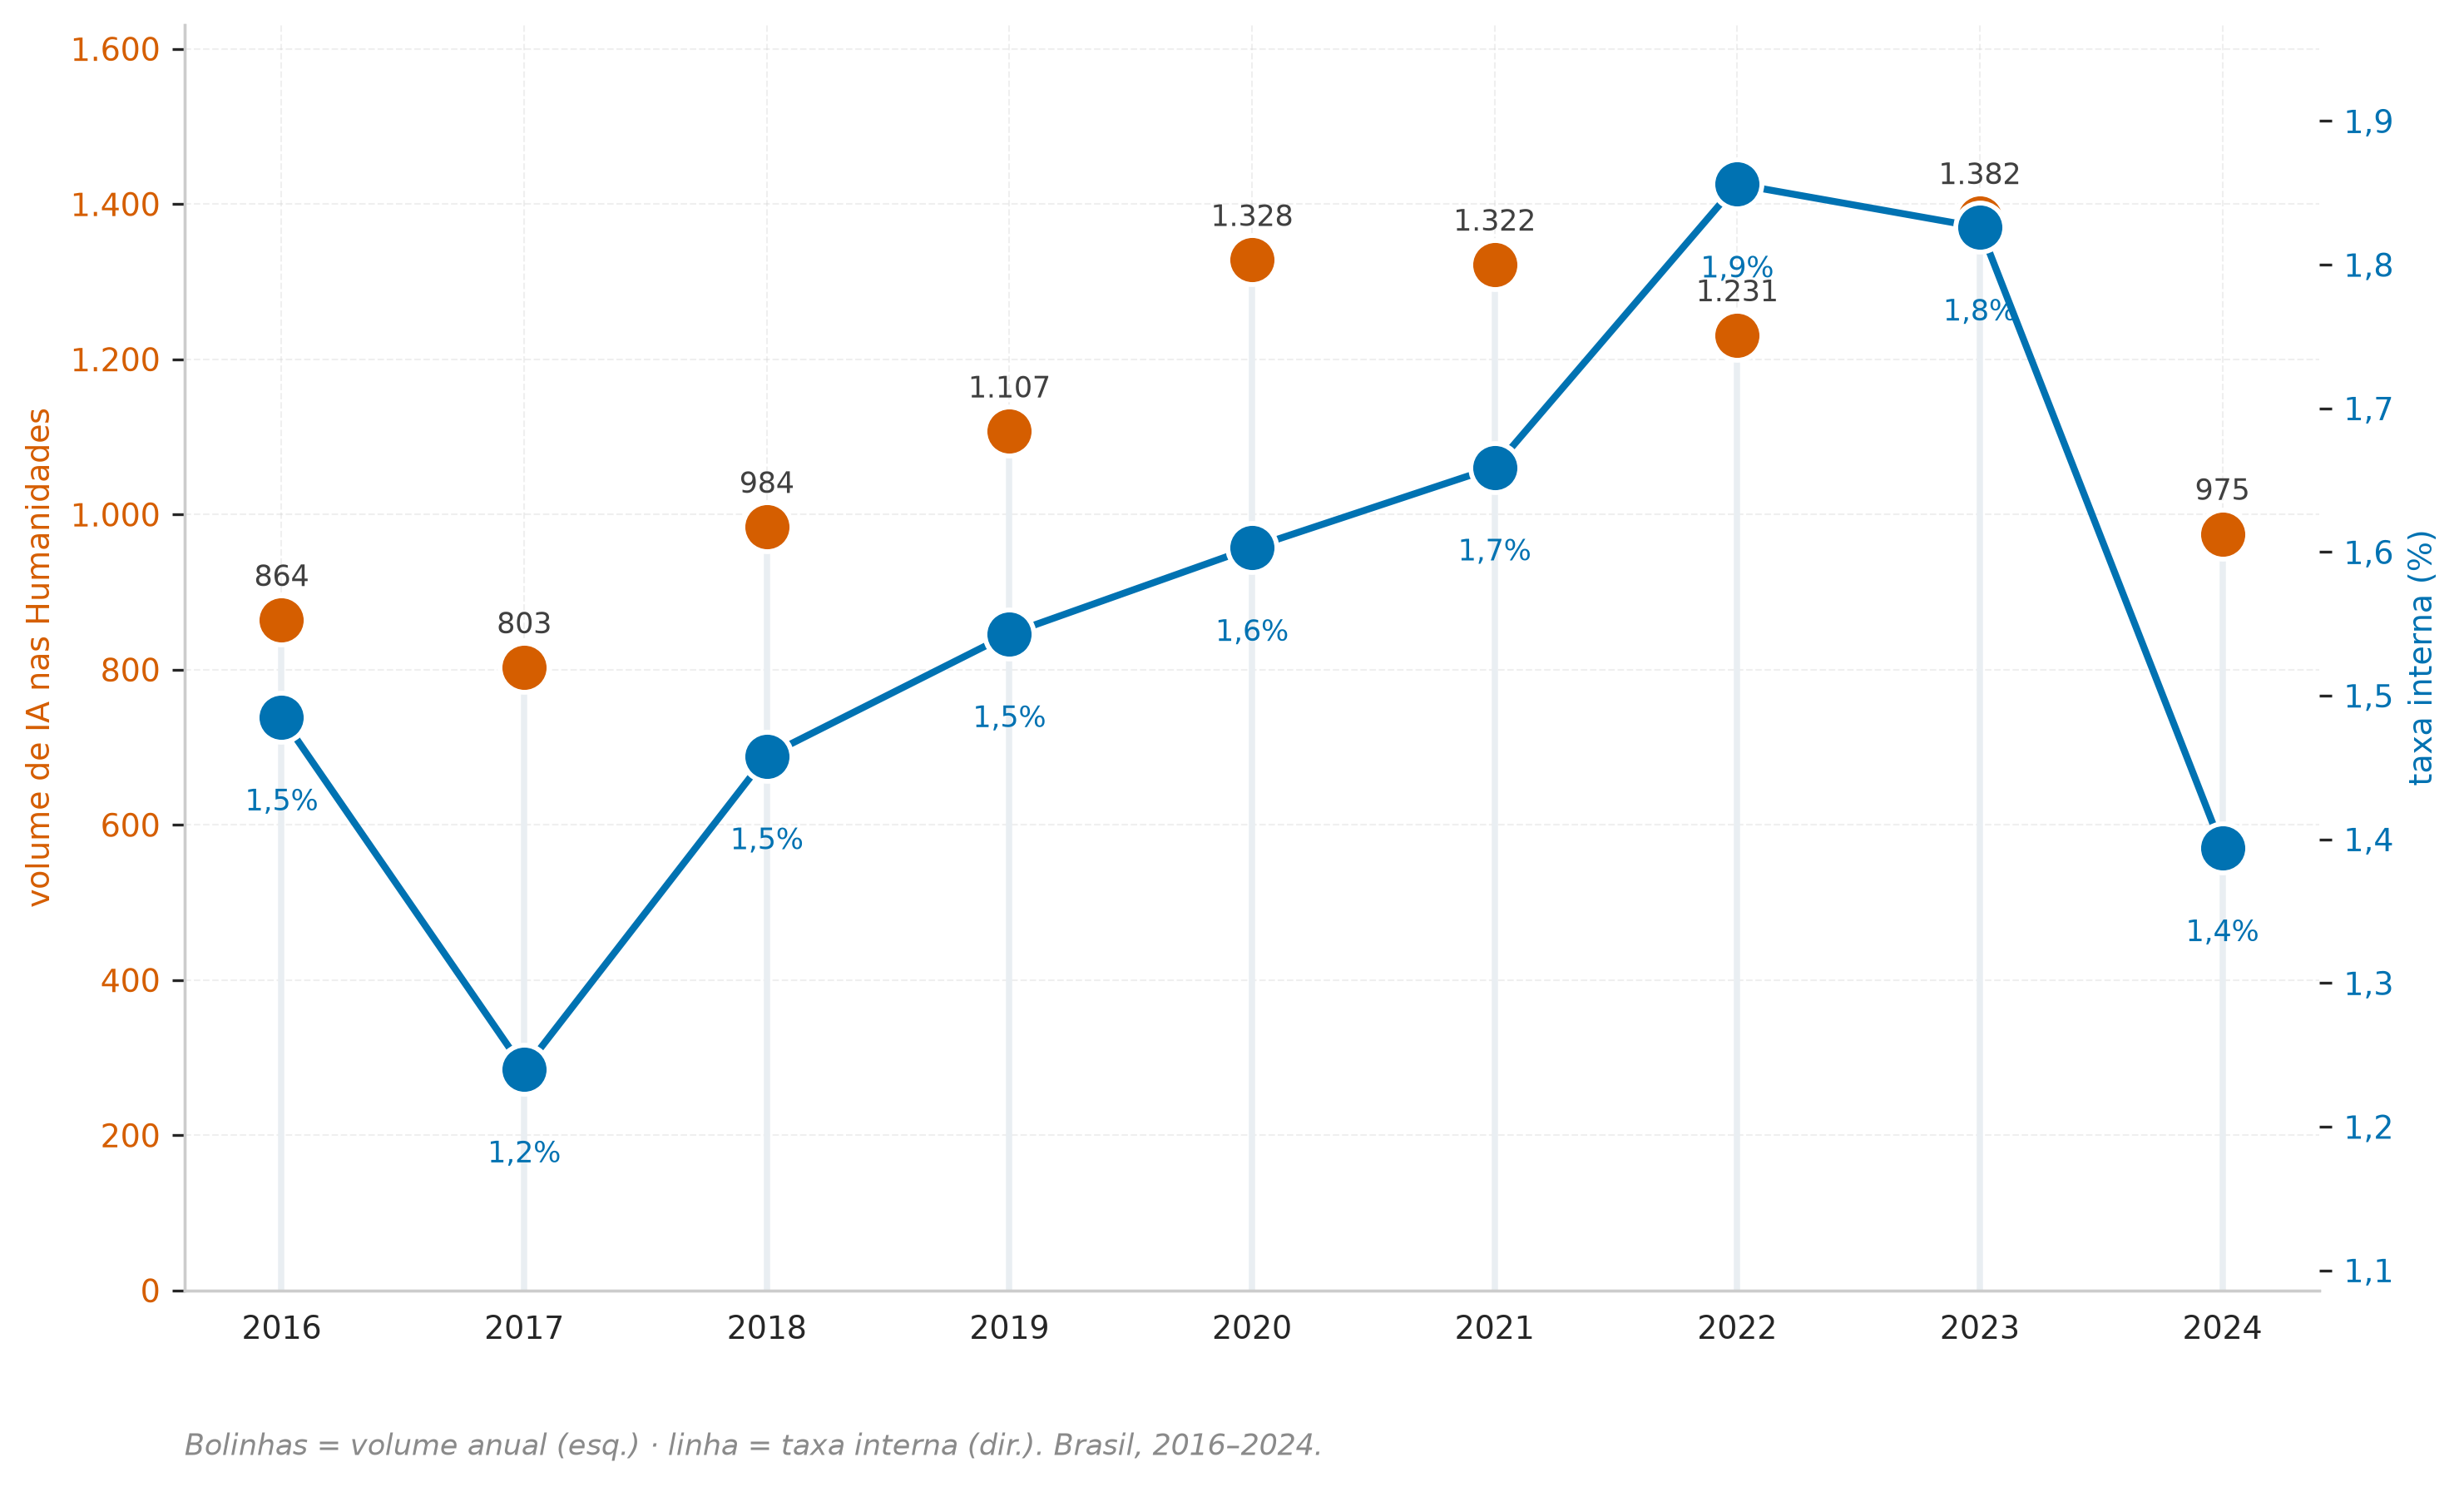
\includegraphics[width=0.85\linewidth]{figuras/cap.2/openalex_03_brasil_temporal.png}
    \caption[Evolução da produção brasileira de IA nas Humanidades, \texttt{OpenAlex} 2016--2024]{%
        Brasil, no período 2016--2024, pela definição por conceito do
        \texttt{OpenAlex}. As bolinhas mostram o volume anual, isto é, o número
        absoluto de obras de Humanidades que tocam a inteligência artificial, e
        a linha mostra a taxa interna, a fração que essas obras representam
        dentro de todas as obras de Humanidades do país no mesmo ano. O volume
        cresce de 864 obras em 2016 para 1.382 em 2023, ao passo que a taxa
        interna se mantém em uma faixa estreita, entre 1,24\% e 1,86\%, com pico
        em 2022. O descompasso entre os pontos que sobem e a linha que não
        acompanha é a leitura central da figura: o Brasil produz mais obras de
        inteligência artificial nas Humanidades a cada ano, sem que a fração das
        Humanidades dedicada ao tema se amplie na mesma medida. A retração
        aparente de 2024, com 975 obras, deve-se com grande probabilidade à
        indexação ainda incompleta do ano na plataforma, e não a um declínio
        real, limitação análoga à que afeta a própria base do \texttt{CSET}.
        Elaboração própria a partir do \texttt{OpenAlex}. Repositório com dados,
        \emph{scripts} e figuras em \protect\url{https://github.com/julianehelanski/bibliometria-ia-humanas}.}
    \label{fig:openalex_brasil_temporal}
\end{figure}

A trajetória brasileira no tempo, na Figura~\ref{fig:openalex_brasil_temporal}, mostra crescimento sustentado entre 2016, com 864 obras, e 2023, com 1.382, acompanhado de uma taxa interna que se move em uma faixa estreita, entre 1,24\% e 1,86\%, com pico em 2022. Leio a queda aparente de 2024, com 975 obras, com cautela, porque o \texttt{OpenAlex} segue indexando as publicações do ano mais recente, de modo que o número está quase certamente subestimado, do mesmo modo que a base do \texttt{CSET}. O que é marcante na curva é a estabilidade da taxa interna em um patamar baixo, e não a flutuação de cada ano: o volume cresce, e a fração das humanidades brasileiras que incorpora a inteligência artificial permanece presa em torno de 1,5\%, o que sugere uma expansão concentrada em poucos nichos, em lugar de uma difusão ampla pelo campo. A aceleração que a \texttt{Capes} e a \texttt{SciELO} registram a partir de 2022 aparece, no \texttt{OpenAlex}, como crescimento de volume sem alargamento da fração, e essa diferença de leitura vem dos recortes distintos das três bases, pois a janela do \texttt{OpenAlex} começa em 2016 e cobre o mundo, ao passo que as duas brasileiras se concentram no quadriênio 2021--2024.

\begin{figure}[htbp]
    \centering
    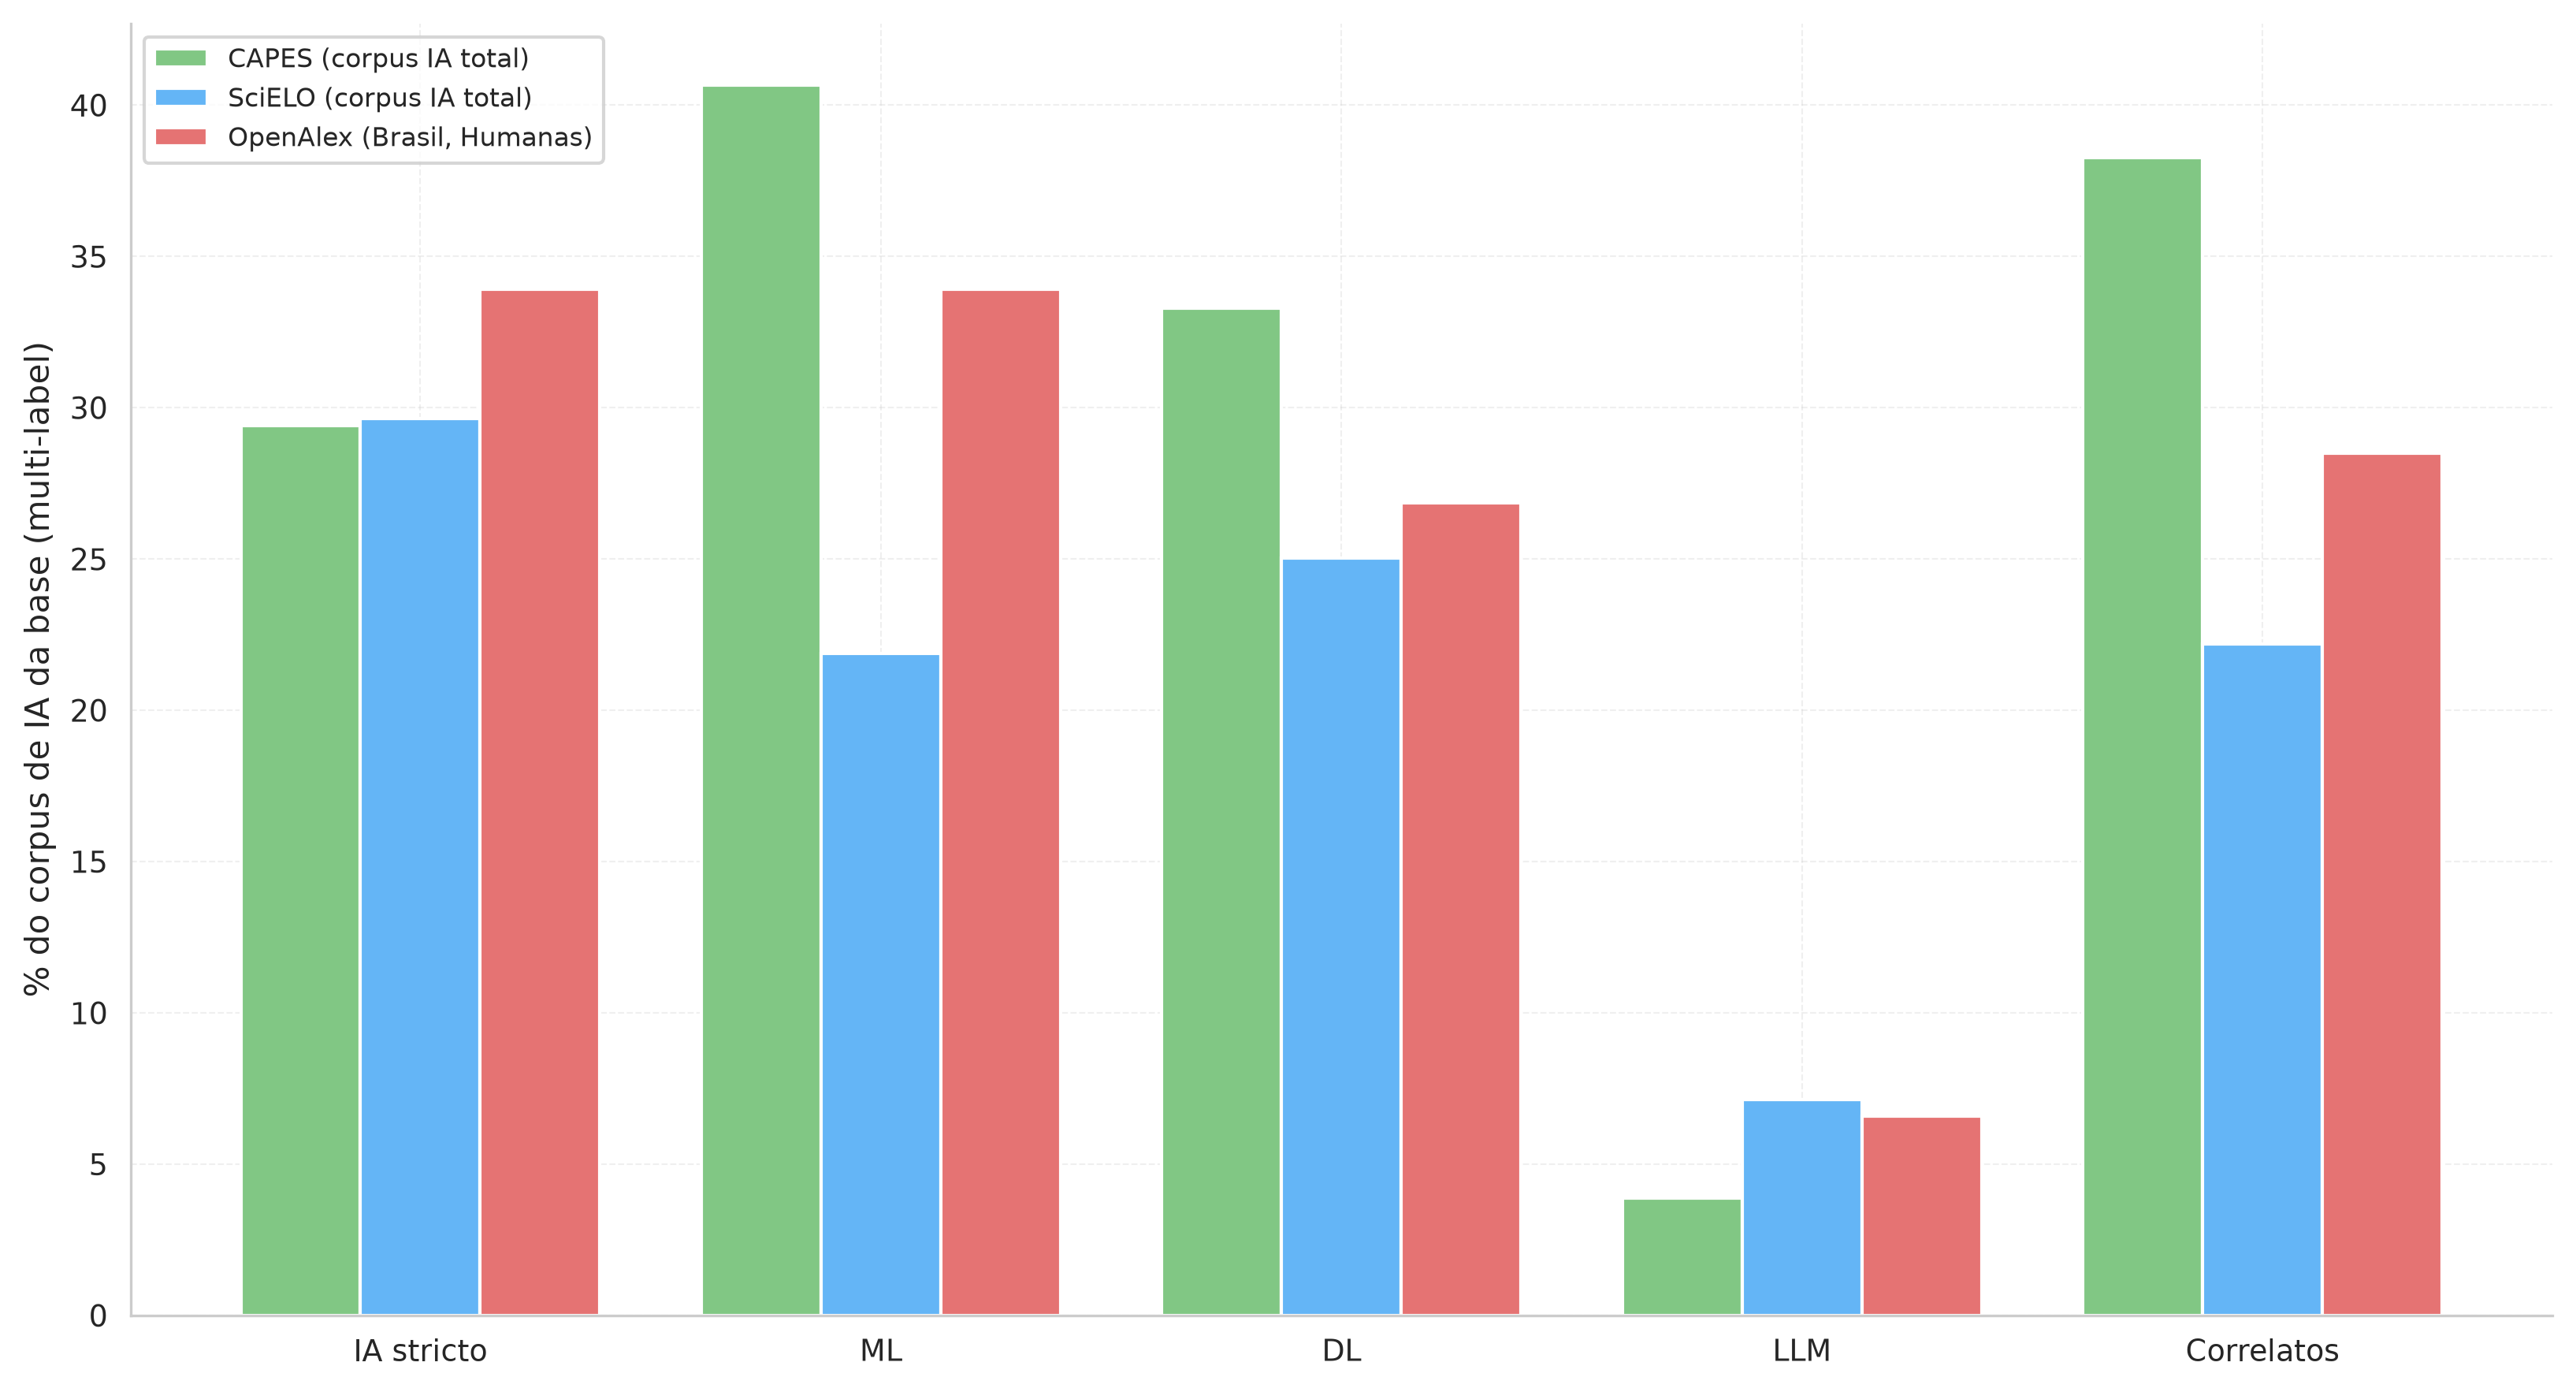
\includegraphics[width=0.85\linewidth]{figuras/cap.2/openalex_04_subcampos_3bases.png}
    \caption[Comparação dos subcampos de IA nas três bases]{%
        Peso relativo dos cinco subcampos da régua de classificação em cada uma
        das três bases. Um mesmo trabalho pode pertencer a mais de um subcampo,
        e por isso a soma dos percentuais ultrapassa cem. Os percentuais da
        \texttt{Capes} e da \texttt{SciELO} se referem ao corpus de inteligência
        artificial total de cada base, e os do \texttt{OpenAlex} ao recorte de
        Humanidades do Brasil pela régua de palavra-chave, e a diferença de
        escopo é declarada no corpo do texto. A hierarquia entre a inteligência
        artificial em sentido estrito e o aprendizado de máquina varia entre as
        três fontes, e os modelos de linguagem e a inteligência artificial
        generativa formam o menor subcampo nas três. Elaboração própria a partir
        do Catálogo de Teses e Dissertações da \texttt{Capes}, da \emph{API}
        ArticleMeta da coleção brasileira da \texttt{SciELO} e do
        \texttt{OpenAlex}. Repositório com dados, \emph{scripts} e figuras em \protect\url{https://github.com/julianehelanski/bibliometria-ia-humanas}.}
    \label{fig:openalex_subcampos_3bases}
\end{figure}

A Figura~\ref{fig:openalex_subcampos_3bases} põe lado a lado o peso dos cinco subcampos nas três bases, e a leitura pede uma ressalva de escopo, porque os percentuais da \texttt{Capes} e da \texttt{SciELO} vêm do corpus de inteligência artificial total de cada base, ao passo que os do \texttt{OpenAlex} vêm do recorte de humanidades do Brasil, pela régua de palavra-chave que torna os três comparáveis. Feita essa ressalva, dois padrões se destacam. O primeiro é que a hierarquia entre a inteligência artificial em sentido estrito e o aprendizado de máquina muda conforme a base, pois na \texttt{Capes} o aprendizado de máquina predomina, com 40,7\% contra 29,4\% da inteligência artificial em sentido estrito, na \texttt{SciELO} a relação se inverte, com 29,6\% contra 21,9\%, e no \texttt{OpenAlex} os dois subcampos empatam, com 33,9\% cada um, os mesmos 288 trabalhos. O segundo é que os modelos de linguagem e a inteligência artificial generativa formam, nas três bases, o menor subcampo, com 3,9\% na \texttt{Capes}, 7,1\% na \texttt{SciELO} e 6,6\% no \texttt{OpenAlex}, indício de que, no período que analiso, a virada generativa ainda não se traduzira em produção acadêmica de vulto nas humanidades, mesmo que já tivesse reorganizado o discurso público sobre a inteligência artificial.

As evidências do \texttt{OpenAlex}, tomadas em conjunto, levam o argumento desta seção para uma escala internacional. A marginalidade da inteligência artificial nas humanidades brasileiras não vem da escassez de produção humanística, porque o Brasil é o segundo maior produtor mundial do conjunto que analiso, e vem da estreita permeabilidade desse campo vasto às tecnologias de inteligência artificial, a menor entre os grandes produtores. Três ressalvas acompanham essa leitura. A primeira é que o \texttt{OpenAlex} privilegia os metadados em inglês, e por isso subestima a produção em português, e também a em chinês, o que afeta de modo desigual justamente o Brasil e a China; essa subestimação, porém, não fragiliza o achado, porque a \texttt{Capes} e a \texttt{SciELO} são bases nacionais, em português, sem viés de idioma, e devolvem a mesma ordem de grandeza baixa, de modo que o diagnóstico se sustenta exatamente onde a cobertura do \texttt{OpenAlex} falha. A segunda é que, na comparação por país, uma obra é somada uma vez para cada país de afiliação de seus autores, e os números brasileiros por obra única corrigem essa dupla contagem, ainda que as comparações internacionais a mantenham por alinhamento à regra do \texttt{CSET}. A terceira é que o ano de 2024 está subindexado. Nenhuma dessas ressalvas desfaz o achado de fundo, que três bases independentes, a \texttt{Capes}, a \texttt{SciELO} e o \texttt{OpenAlex}, reiteram por caminhos separados, e as três oferecem a possibilidade de retomar o levantamento futuramente e conferir o ritmo da emergência e refinar a categorização e a triagem que aqui apresentei.

A análise lexicométrica das três bases mede um campo cuja paisagem qualitativa tem percurso próprio, anterior ao adensamento recente que os números registram, e interpreto uma parte da escassez que elas medem como efeito de cobertura, dado que nenhum recorte bibliométrico, nem o da \texttt{Capes}, nem o da \texttt{SciELO}, nem o do \texttt{OpenAlex}, alcança a produção que circula em livros, capítulos e anais fora das bases indexadas. Há, porém, um limite mais profundo que o da cobertura, e que a bibliometria não tem como medir: ela conta o que se nomeia como inteligência artificial em um recorte recente, e por isso não enxerga o pensamento que vinha tratando a técnica sob outros nomes, a cibernética e o pós-humano, muito antes de a inteligência artificial se tornar o termo que organiza o debate. É a partir daqui que deixo de ler os números e passo a ler o terreno como ele se apresenta a mim, e reúno, à frente, os interlocutores que escolho para situar a minha pesquisa nessa tradição. Reconheço o primeiro deles em Laymert Garcia dos Santos, que, entre os primeiros a investigar sistematicamente as implicações políticas da tecnologia no Brasil, desenvolve desde os anos 1980 um percurso que vai da revolução cibernética ao pós-humano \parencite{Santos_2005_Entrevista, Santos_2022_SociologiaNaoAutocratica}. Seguindo a proposta de Garcia dos Santos uma ressonância que reencontro em trabalhos mais recentes como o de Diego Vicentin, que examina os desafios de aprofundar reflexões sobre inteligência artificial e de encontrar seu sentido ético pela noção de tecnologia de Gilbert Simondon em diálogo com os estudos críticos recentes sobre inteligência artificial \parencite{Vicentin_2022_Esboco}. A mesma preocupação atravessa as reflexões de Pedro Peixoto Ferreira sobre o que significa ser humano na era da inteligência artificial, pela análise do CAPTCHA (\textit{Completely Automated Public Turing Test To Tell Computers and Humans Apart}), em que ele sustenta que o CAPTCHA, ainda que nominalmente seja um sistema de segurança para distinguir humanos de computadores, funciona na prática como mecanismo de servidão maquínica e sujeição social, e recruta trabalho humano não remunerado para treinar sistemas de inteligência artificial das \textit{Big Techs} \parencite{Ferreira_2025_NaoSouUmRobo}.

A reflexão sobre as implicações éticas, estéticas e sociais das tecnologias de inteligência artificial aparece também em estudos antropológicos em diálogo com as artes visuais. Giselle Beiguelman investiga como a imagem digital, das \textit{selfies} aos \textit{memes}, dos \textit{deep fakes} à \textit{IoT}, tornou-se mediadora das relações sociais e campo de tensões políticas contemporâneas, e produz uma estética da vigilância impulsionada pela produção massiva de dados e imagens por meio de \textit{smartphones} \parencite{beiguelman2021}. Em diálogo com as artes visuais, Beiguelman usa inteligência artificial generativa (\texttt{DALL-E} e \texttt{Runway}) para criar imagens e vídeos que resgatam a história de mulheres e plantas estigmatizadas e proibidas ao longo do tempo, e toma a inteligência artificial como espaço de crítica e meio de problematização estética dos padrões de representação que os dados da tecnologia tendem a reproduzir \parencite{Beiguelman_2025_Venenosas}.\footnote{A exposição de Giselle Beiguelman pode ser visitada em: \url{https://venenosas.desvirtual.com}. Acesso em: 6 nov.~2024.} Dossiês de revistas acadêmicas acompanham esse movimento, e exploram as confluências entre pesquisa antropológica e interações entre humanos, transumanos e máquinas não humanas.\footnote{Iniciativa que aparece em dossiês de revistas como \enquote{Tecnopoéticas, Inteligência Artificial, maquinações e outras bricolagens}, cujos artigos exploram confluências e pontos de fricção entre pesquisa antropológica, processos narrativos e interações entre humanos, transumanos e máquinas não humanas \parencite{Magni_2024_Apresentacao}. Os artigos do dossiê estão disponíveis em: \url{https://seer.ufrgs.br/index.php/iluminuras/issue/view/5143}. Acesso em: 6 nov.~2024.}

A popularização da inteligência artificial generativa a partir de 2022 funcionou como vetor de atenção para as ciências sociais, e o que antes circulava em áreas especializadas tornou-se objeto de uso cotidiano, e ampliou o escopo das perguntas sobre o que são essas tecnologias e suas implicações para a sociedade. Trabalhos recentes abordam a propagação de \textit{deep fakes} e \textit{fake news}, as desigualdades socioeconômicas intensificadas pela inteligência artificial na educação, a análise psicanalítica da pós-humanidade e a xenoantropologia das máquinas como perspectiva para enfrentar a fusão das fronteiras entre espécies e artefatos.\footnote{A presença da tecnologia como objeto de debate pode ser aferida pela programação dos principais eventos das ciências sociais brasileiras e do Mercosul. Na XV Reunião de Antropologia do Mercosul (RAM), realizada em Salvador em agosto de 2025, com aproximadamente 178 grupos de trabalho, apenas 1 nomeia inteligência artificial diretamente no título: o GT~146 (\enquote{Perspectivas antropológicas sobre plataformas digitais, extrativismo de dados e inteligência artificial}, coordenado por Carolina Parreiras, Patricia Pereira Pavesi e Cecilia Melella); outros 10 GTs abordam tecnologia, digital ou dados de modo mais amplo, entre os quais o GT~023 (\enquote{Antropologia Digital e Tecnologias Contemporâneas}), o GT~011 (\enquote{Antropologia da ciência e da tecnologia em perspectiva}), o GT~027 (\enquote{Antropologia dos dados e das práticas de quantificação}) e o GT~078 (\enquote{Digitalización de la vida cotidiana y producción de conocimiento en América Latina}); 3 mesas redondas e 1 oficina completam esse escopo, entre as quais a MR~61 (\enquote{Pesquisa e redes sociais em tempos de \textit{TechBros} e Tecnofascismos: perspectivas feministas}) e a OF~37 (\enquote{Tecnologia, natureza, imaginação e trabalho abstrato: sistemas ciberfísicos como exemplo para uma teoria e prática críticas nos estudos sociotécnicos}). No 49º Encontro Anual da ANPOCS, realizado na \texttt{Unicamp} em outubro de 2025, com 68 grupos de trabalho e 31 mesas redondas presenciais, 1 GT e 1 mesa redonda nomeiam inteligência artificial diretamente: o GT~56 (\enquote{Inteligência Artificial, Sociedade, Cultura e Poder}) e a MR~20 (\enquote{Plataformas Digitais, IA e Sociedade: Desafios para as Ciências Sociais}); outros 5 GTs abordam tecnologia e plataformas digitais, entre os quais o GT~61 (\enquote{Pesquisa social com mídias e plataformas digitais}) e o GT~11 virtual (\enquote{Estudos Sociais da Ciência e da Tecnologia}). Na 35ª Reunião Brasileira de Antropologia (RBA), realizada em Goiânia em julho de 2026, com aproximadamente 118 grupos de trabalho, 73 mesas redondas e 24 simpósios especiais, nenhum espaço nomeia inteligência artificial diretamente no título; 4 GTs abordam tecnologia e o digital: GT~015 (\enquote{Antropologia da Técnica}), GT~017 (\enquote{Antropologia das ciências, tecnologias e outras ancestralidades}), GT~020 (\enquote{Antropologia digital e políticas etnográficas}) e GT~021 (\enquote{Antropologia digital: debates teóricos, metodológicos, éticos e políticos}); 2 simpósios especiais tratam de digitalização e algoritmos: SE~09 (\enquote{Entre pluralidade de saberes, descolonização e algoritmos}) e SE~11 (\enquote{Fazer e comunicar antropologia em tempos de plataformas e digitalização}); e 1 mesa redonda aborda o subcampo: MR~63 (\enquote{Perspectivas e caminhos da antropologia digital no Brasil}). As programações completas estão disponíveis em: \url{https://www.xvram.com.br} (acesso em: 5 abr.~2026), \url{https://anpocs.org.br/49-encontro-anual} (acesso em: 5 abr.~2026) e \url{https://www.rba2026.com.br} (acesso em: 5 abr.~2026).}

A produção de \enquote{etnografias do digital}\footnote{Tema da edição 68, v.~30 da \textit{Revista Horizontes Antropológicos} organizada por Jean Segata, Theophilos Rifiotis e Maria Elisa Máximo. A edição está disponível em: \url{https://seer.ufrgs.br/index.php/horizontesantropologicos/issue/view/5110/1484}. Acesso em: 6 nov.~2024.} acompanhou esse movimento de expansão, e expõe a diversidade de análises do digital e a sua presença na vida cotidiana. As ciências sociais vêm questionando a ideia de sociedade como reunião apenas de humanos, e consideram coletivos formados por moléculas, códigos binários e dados algoritmicamente minerados, tecnologias que, ainda que globais em alcance, encontram resistências e se transformam em práticas locais. Computadores, \emph{softwares}, aplicativos, redes sociais, algoritmos, DNA, inteligência artificial e organismos geneticamente modificados formam um amálgama que costura tecnologias digitais e da vida, e desenham mundos múltiplos e futuros já presentes, ainda que desigualmente distribuídos \parencite{Rifiotis2024Etnografias}. Essa paisagem qualitativa não contradiz a escassez que as três bases medem, e a precede e a contextualiza, porque mostra que a antropologia brasileira vinha pensando a técnica e o digital muito antes de a inteligência artificial se tornar objeto de estudo desta tese, de artigo e de grupo de trabalho. A defasagem que a bibliometria registra é, então, menos a ausência de um pensamento sobre a tecnologia e mais como que esse pensamento se volta para a inteligência artificial como tema de pesquisa. É nessa dobra que situo a minha pesquisa, entre uma tradição que já existe e um objeto de estudo ainda em emergência.

\section{Arremate: figurações e análise computacional}
\label{sec:revisao_etnografia}

Abri o capítulo~\ref{capitulo2} com duas epígrafes e duas figuras postas lado a lado, a do exército de aliados de Latour e a do berço de gato de Haraway, porque em Haraway a figuração propõe e põe em jogo padrões. Os padrões são formas que emergem da relação e que pedem resposta, e obrigam a fazer algo com elas. Exigem receber e passar, pegar e largar, e por isso são coletivos e relacionais, e podem ser jogados tanto por humanos quanto por não humanos, desde que o ritmo entre dar e receber se mantenha. Porque propõem jogos, esses padrões são mais propositivos do que descritivos, e apresentam modos possíveis de relação, aquilo que \textcite{Haraway2023Ficar} chama de tornar-se-com e fazer-com, a simpoiese. É essa dupla natureza que separa a figuração de Haraway da figuração militar de Latour. O exército de aliados descreve como a tecnociência funciona, ao passo que o jogo da figura de barbante descreve como ela funciona e, no mesmo gesto, propõe que poderia funcionar de outro modo. Pôr as duas figuras em relação é, ele mesmo, um gesto de figurar, o de passar um fio de uma mão a outra para ver que forma se sustenta entre elas \parencite[p.~25]{Haraway2023Ficar}. As duas dão a ver, portanto, duas maneiras de pôr as coisas em relação no fazer-conhecimento: de um lado, o autor cercado de aliados, em que a relação acumula reforços e se mede pela controvérsia que vence; de outro lado, as mãos entrelaçadas por um fio compartilhado, em que a relação só persiste enquanto há quem a receba e devolva, sem \textit{front} e sem adversário.

Convocar autores e alistá-los para sustentar uns argumentos, contestar outros e acumular reforços contra o ataque deriva das figurações que \textcite[cap.~1]{Latour2011CienciaEmAcao} elaborou para explicar a produção tecnocientífica, ao lado de outras figurações menos confrontativas. Escolhi ficar com as figurações de \textcite{latour_woolgar_1986_lab_life} e \textcite{latour1996clarifications, Latour1999RecallingANT, Latour1987Science, Latour1999PandorasHope, Latour2013Inquiry}, ao lado das figurações de Haraway e de Stengers, que tomam o conhecimento como prática de pôr as coisas em relação por outros caminhos, a trama multiespécie e a desaceleração do pensamento. Justifiquei nessa abertura o recorte do corpus, e expliquei que o recorte antecede a análise lexicométrica em vez de ser montado para ela, porque a figuração militar-industrial já era objeto da pesquisa antes disso, sustentada pela leitura e pelo uso desses termos na construção da tese, e a análise veio depois, para dar base à leitura interpretativa que eu já vinha fazendo. É essa tensão entre alistar e tecer que levo adiante, não para resolvê-la, mas a partir dela, tramar com as figurações da/na tecnociência nos capítulos seguintes.

A seção~\ref{sec:analise_lexicometrica} apresentou a análise lexicométrica das figurações, que desenvolvi com o \texttt{claude} e o \texttt{claude code} sobre seis obras de Latour publicadas entre 1986 e 2013. A análise lexicométrica abrangeu um conjunto de procedimentos que processa um corpus textual com métodos estatísticos e computacionais, identifica frequências, distribuições e relações de co-ocorrência entre as palavras, e preserva, pelo procedimento de \emph{keyword in context}, o vínculo de cada ocorrência com a sua vizinhança textual. O número de ocorrências de um rótulo foi o ponto de partida da análise. Organizei-a em três etapas, e a razão dessa divisão é que cada etapa pergunta o que acontece com as figurações quando muda o objeto que Latour descreve. A etapa~1 processou os três livros (\emph{Laboratory Life}, de Latour e Woolgar, de 1986, \emph{Science in Action}, de 1987, e \emph{Pandora's Hope}, de 1999) e mediu a densidade do rótulo \texttt{militar} em cada um deles. A densidade é baixa em \emph{Laboratory Life}, salta em \emph{Science in Action} e permanece alta em \emph{Pandora's Hope}. Dessa forma, a análise textual forneceu um outro contexto que complementou a leitura e as aplicações que eu vinha fazendo das obras nesta tese. A etapa~2 estendeu a análise aos dois artigos metateóricos (\emph{Clarifications}, de 1996, e \emph{On Recalling ANT}, de 1999), e fiz isso porque, se o vocabulário militar satura a escrita com que Latour descreve a tecnociência, era razoável esperar que ele se reorganizasse quando Latour, de modo autorreflexivo, reinterpreta a própria teoria; o que a análise mostrou foi a queda do rótulo \texttt{militar} e a dominância dos rótulos \texttt{topologia} e \texttt{textil}, que acrescentei ao catálogo justamente para captar o vocabulário têxtil-topológico que a leitura qualitativa desses dois artigos havia revelado. A essa etapa somei uma validação amostral semântica, em que classifiquei ocorrência a ocorrência em uso figural, parcialmente figural ou não-figural, para distinguir o uso figurativo do uso polissêmico ou citacional e sustentar a inversão de registro já no plano figural depurado, e não apenas no plano lexical bruto. A etapa~3 processou \emph{An Inquiry into Modes of Existence}, de 2013, obra em que apliquei dois catálogos em paralelo, e registrou a reentrada moderada do vocabulário militar agora articulado a objetos cosmopolítico-diplomáticos, com a pendência declarada da desambiguação refinada das suas ocorrências. A subseção~\ref{subsec:costurando_figuracoes} reuniu o que as três etapas mostram: a figuração militar-industrial é uma figuração situada, que aparece de modo seletivo conforme o objeto descrito, e o vocabulário têxtil-topológico, que reconheço como figuração feminista a partir de Haraway, é uma figuração que o próprio Latour compõe nos seus momentos autorreflexivos.

Entre a análise lexicométrica e o mapeamento bibliométrico, percorri as leituras que atravessei ao longo do doutorado, e as dispus na ordem em que cada problema empírico do meu campo as convocou. A seção~\ref{sec:estudos_ciencia_tecnologia} situou a pesquisa nos estudos sociais da ciência e da tecnologia e nos estudos do digital, e marquei ali a tradição antropológica da técnica que corre em paralelo à genealogia sociológica do campo, de Mauss e Lévi-Strauss à filosofia da técnica de Simondon e Hui, além do princípio de não-centramento no digital de Pink, Horst e Postill, que tomo como recorte do objeto. A seção~\ref{sec:etnografias_ia_mediacao} reuniu as primeiras pesquisas antropológicas e sociológicas sobre inteligência artificial, a antropologia de Diana Forsythe e a sociologia dos sistemas especialistas de Harry Collins, e desenvolveu o conceito de mediação técnica que Latour formula em \emph{Pandora's Hope}, revisitado à luz dos sistemas de inteligência artificial generativa; fiz esse percurso porque é o conceito de mediação técnica que me permite descrever o \texttt{claude} e o \texttt{claude code} como actantes que se transformam e transformam os modos de produção tecnocientíficos, de fazer-conhecimento. A seção~\ref{sec:predicao_poder} fez um apanhado das genealogias críticas do poder tecnológico, de Kate Crawford a Matteo Pasquinelli e Vladan Joler, em diálogo com as inflexões brasileiras dessas perguntas, e firmou a postura de descrição que sustento, a de descrever as redes da inteligência artificial sem afundar na denúncia que só vê extração nem na celebração que só vê solução. 

A seção~\ref{sec:emergencia_campo_brasileiro} apresentou o mapeamento bibliométrico do campo brasileiro de estudos em inteligência artificial nas ciências humanas e sociais, que fiz com o \texttt{claude} e o \texttt{claude code} sobre três bases, o Catálogo de Teses e Dissertações da \texttt{Capes}, a coleção brasileira da \texttt{SciELO} e a base internacional \texttt{OpenAlex}. Tomei a \texttt{Capes} como base principal porque um campo em formação inscreve-se primeiro na pós-graduação, na tese e na dissertação, e complementei a sondagem com a \texttt{SciELO} e com o \texttt{OpenAlex} para confrontar o recorte nacional com o periódico e com o recorte internacional. Por busca padronizada de termos-chave, categorização do material retornado em subcampos e leitura situada dos dados, o mapeamento registrou em forma quantificada uma emergência tardia e tematicamente deslocada dos estudos brasileiros sobre inteligência artificial, e estudos sobre tecnologia em geral, marginalidade que se confirma da pós-graduação ao periódico e do recorte nacional ao internacional, e que interpreto menos como ausência de pensamento sobre a tecnologia e mais como uma defasagem do vocabulário com que esses estudos delimitam a inteligência artificial e tecnologias correlatas do mesmo universo. Esse mapeamento surgiu da necessidade de situar esta tese e de mensurar os modos e os ritmos pelos quais a área se aproxima da inteligência artificial como tema e objeto de estudo.

As duas linhas de trabalho deste capítulo~\ref{capitulo2} entregam para os capítulos seguintes três coisas que serão retomadas. A primeira é o reconhecimento de que a figuração com que se descreve a tecnociência é parte do que se descreve, e por isso o tratamento das figurações na obra de Latour, Latour e Woolgar (e também com Haraway e Stengers) como objetos etnográficos, que desenvolvi com o \texttt{claude} e o \texttt{claude code}, abre o caminho que os capítulos~\ref{capitulo3} e~\ref{capitulo4} repetem em outras escalas. A segunda é a tensão entre alistar e aliar, que percorre este capítulo no plano da composição da literatura e que se redistribui, nos próximos capítulos, no plano da composição do campo: alistar aliados teóricos é gesto homólogo ao que Fábio e Cláudio fazem para sustentar o \texttt{C4AI} e ao que Marcelo faz para sustentar o \texttt{Spira}, e descrever esse gesto teórica e empiricamente é parte do que a tecno-etnografia faz. A terceira é a posicionalidade não-inocente que essa tensão exige reconhecer, e a postura de descrição que dela decorre, a de ficar com o problema. O capítulo~\ref{capitulo3} investiga a rede que Fábio e Cláudio construíram ao longo de cinco anos de parceria \texttt{C4AI}-\texttt{IBM}, e a descreve pela sua extensão no tempo, da genealogia corporativa desde Hollerith, em 1890, à dissolução da parceria em dezembro de 2025; o capítulo~\ref{capitulo4} examina a rede que Marcelo construiu com o \texttt{Spira}, e a descreve pela densidade material da cadeia de translações que converteu a voz de pacientes com insuficiência respiratória em espectrogramas, coeficientes e artigos científicos. As duas redes são extensas, cada uma à sua maneira, e voltam a se cruzar no ponto em que a dissolução da parceria e a falha de generalização do modelo expõem a fragilidade do que parecia estável e a proximidade do que parecia distantes.

% ===== Inscrições \texttt{InfraNodus} / trajetória narrativa do capítulo 2 (inserido automaticamente — ajustar posição e prosa) =====
\medskip

A análise de rede textual deste capítulo, no mesmo procedimento descrito no capítulo~\ref{capitulo1}, produziu seis inscrições: três vistas sincrônicas da rede de co-ocorrência (rede completa, núcleo por \textit{degree} e núcleo por critérios informacionais) e três vistas diacrônicas da trajetória dos conceitos ao longo da leitura (Gantt lexical, fluxo aluvial e trajetória semântica), reunidas a seguir.

\begin{figure}[H]
\centering
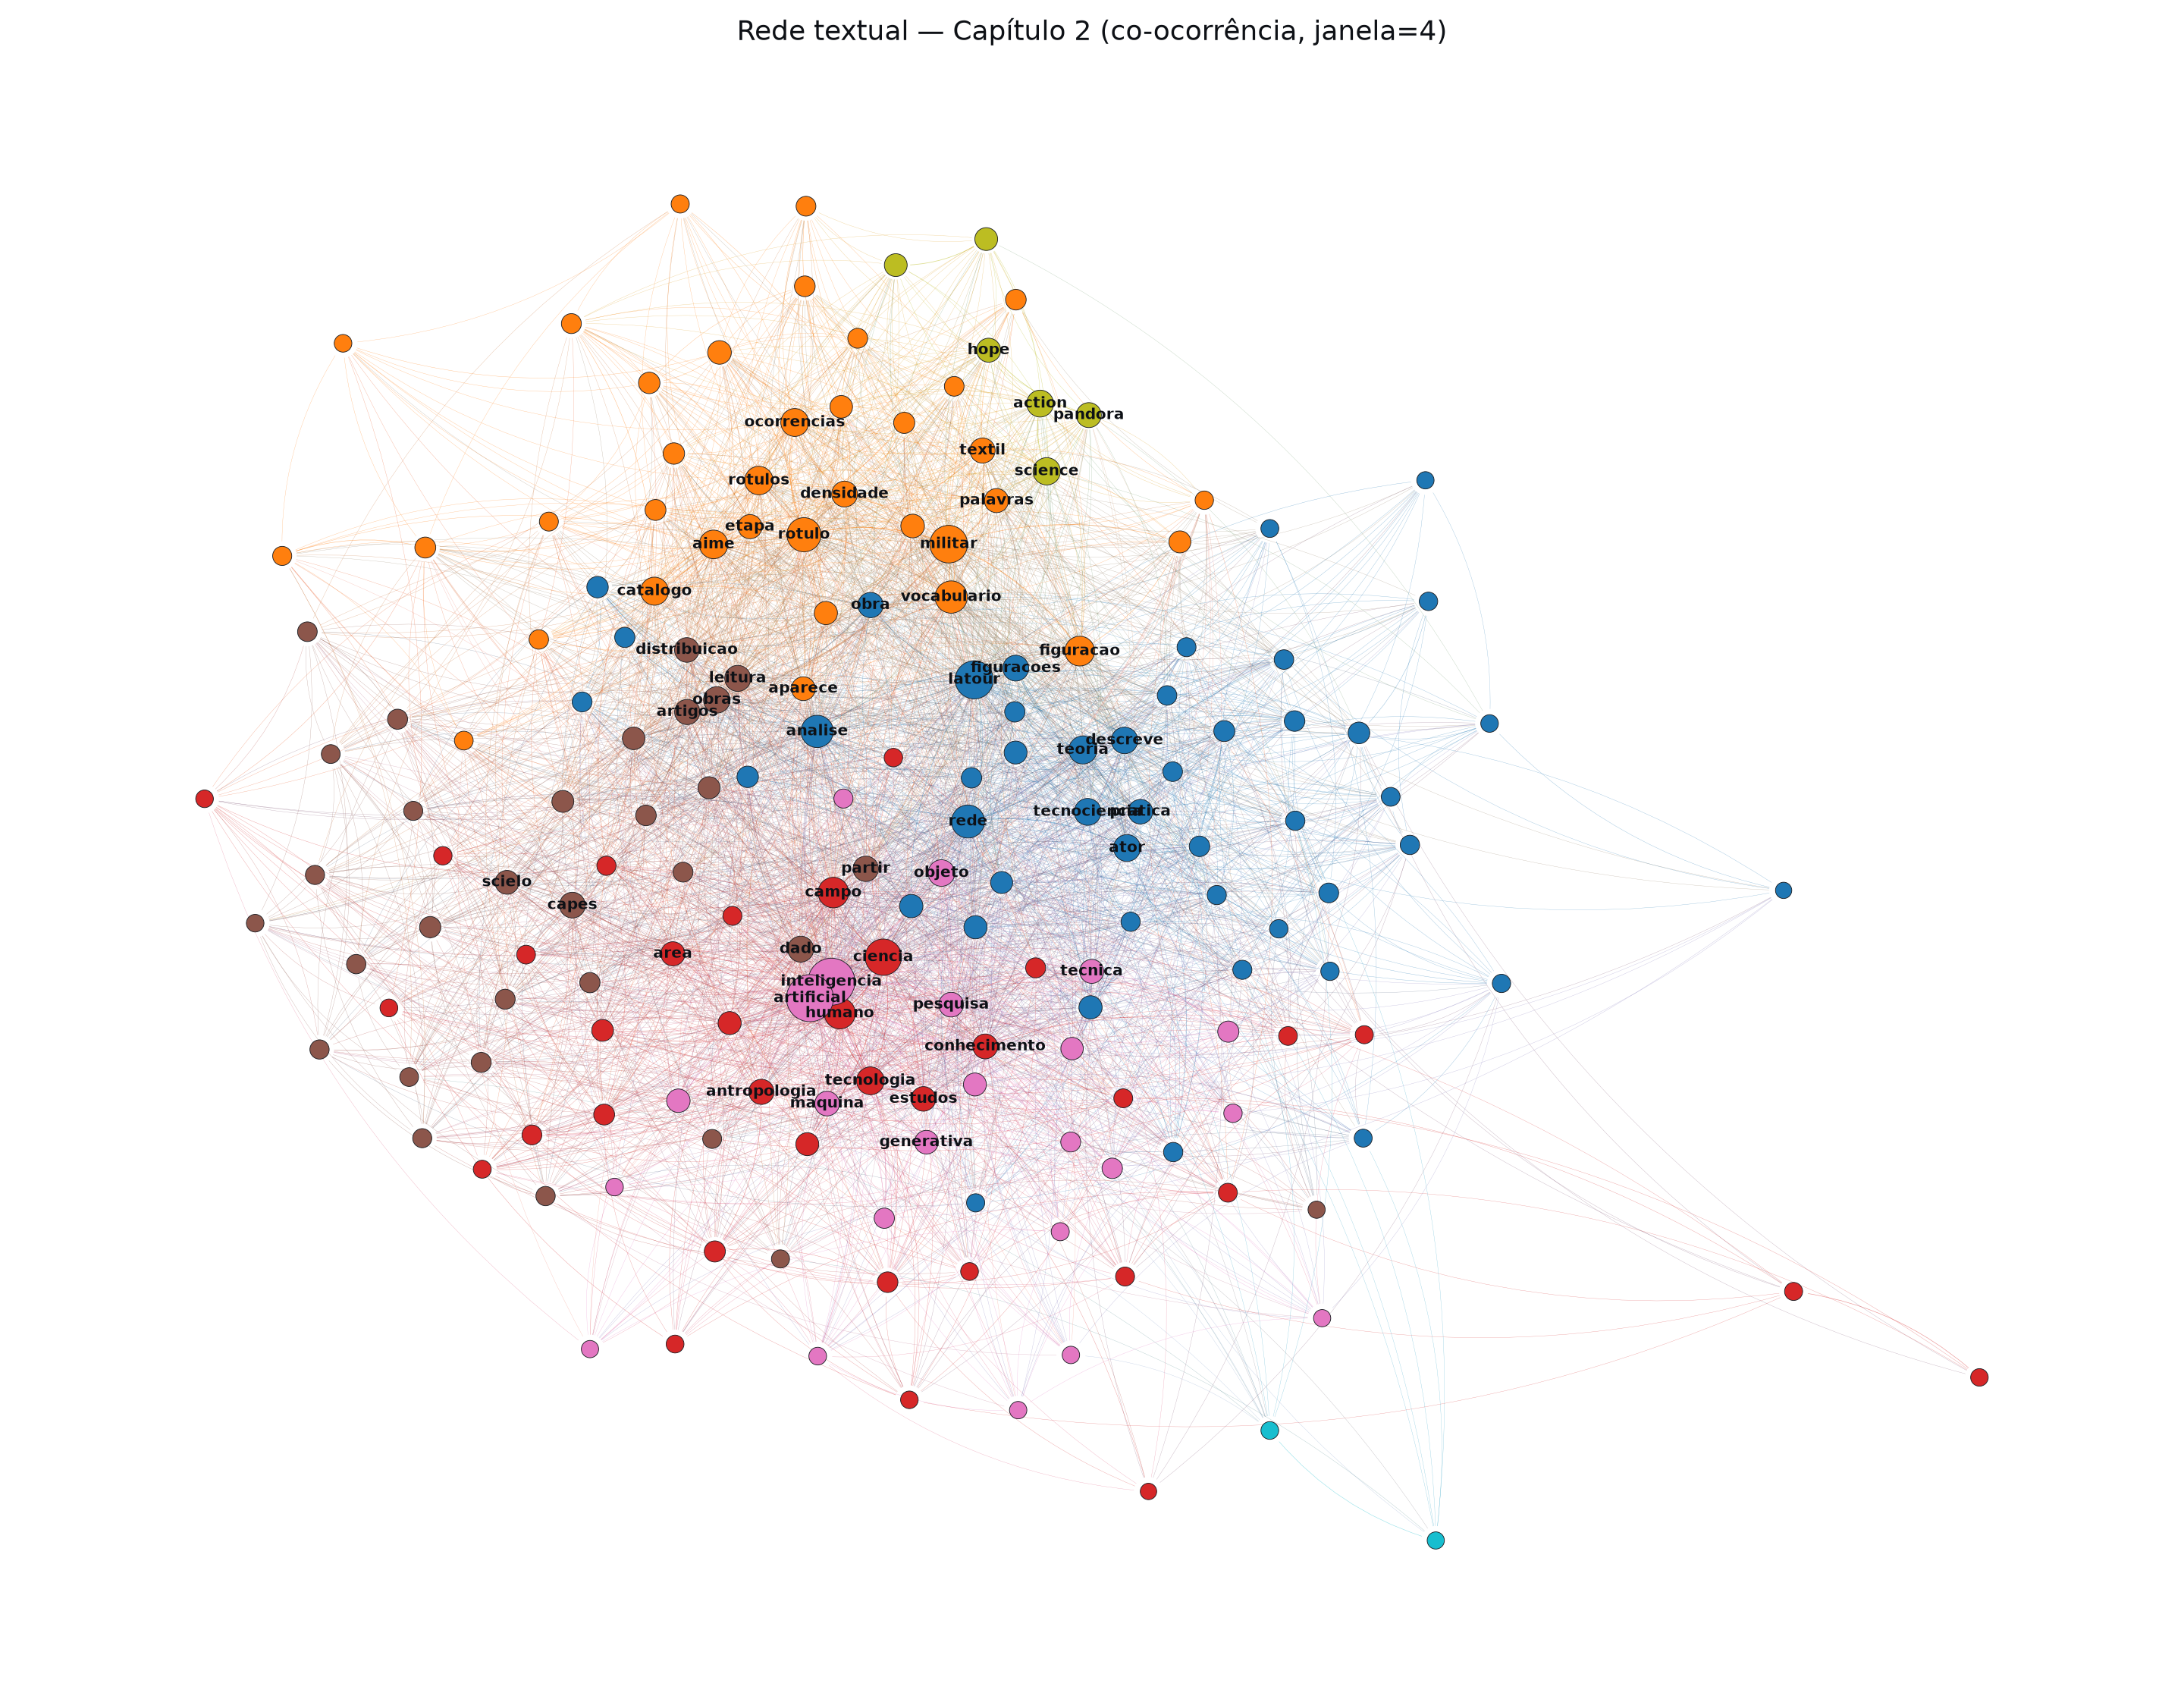
\includegraphics[width=1.0\textwidth,keepaspectratio]{figuras/cap.2/infranodus_cap2_network.png}
\caption[Rede textual completa do capítulo~\ref{capitulo2} (análise de rede textual)]{Rede textual completa do capítulo~\ref{capitulo2}. O grafo resulta de janela deslizante de 4 \textit{tokens} sobre o texto pré-processado (remoção de \textit{stopwords}, comandos \LaTeX, lematização leve), com pesos decrescentes pela distância (3-2-1). Os nós são os 180 termos de maior frequência mantidos no maior componente conectado após a filtragem de arestas com peso $<2$; o tamanho do nó é proporcional ao \textit{degree} ponderado e a cor indica a comunidade detectada por Louvain ponderado; as arestas, arqueadas, recebem a mistura das cores das comunidades que ligam. Esta vista privilegia a estrutura geral do capítulo, incluindo termos periféricos e pontes entre tópicos. Arquivos auxiliares (\texttt{.gexf} para \texttt{Gephi}, CSVs, métricas e relatório) no repositório \url{https://github.com/julianehelanski/tecno-etnografia-centro-ia}.}
\label{fig:infranodus-cap2-network}
\end{figure}

\begin{figure}[H]
\centering
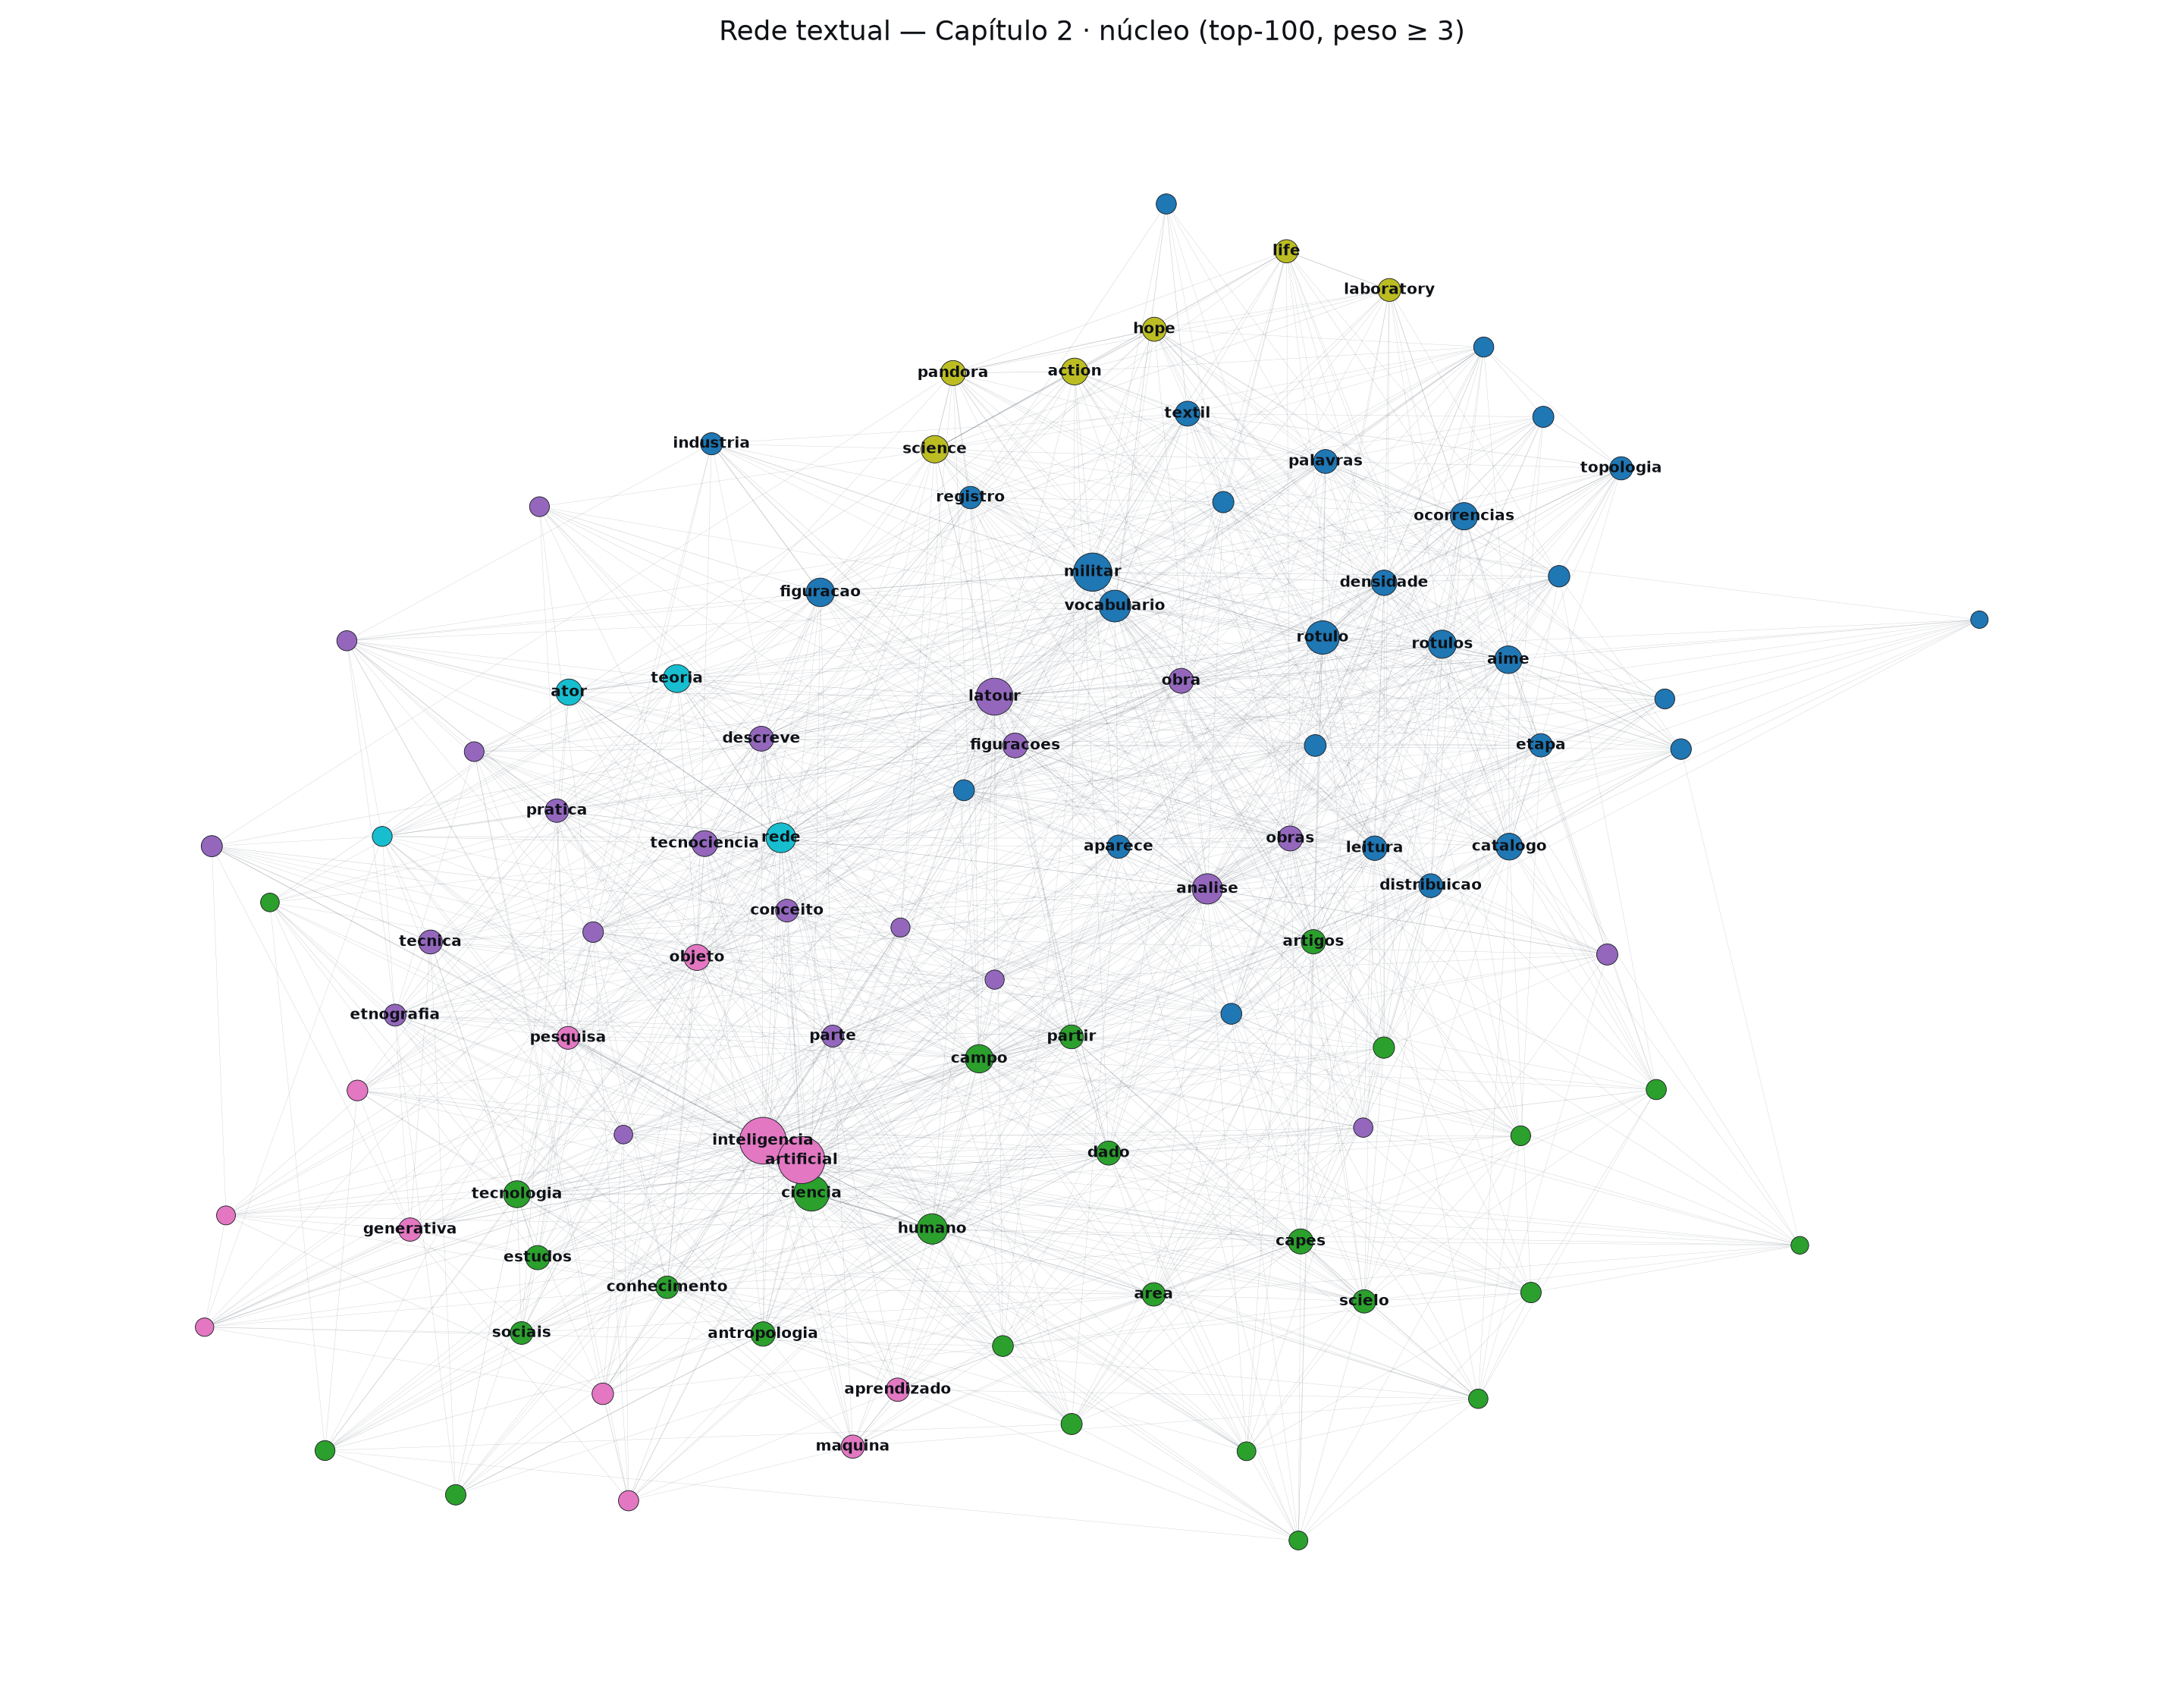
\includegraphics[width=1.0\textwidth,keepaspectratio]{figuras/cap.2/infranodus_cap2_focus.png}
\caption[Núcleo da rede textual do capítulo~\ref{capitulo2} (análise de rede textual)]{Núcleo da rede textual do capítulo~\ref{capitulo2} (análise de rede textual). Os nós são os 100 termos com maior \textit{degree} ponderado; o tamanho do nó é proporcional ao \textit{degree}; a cor indica a comunidade detectada por Louvain ponderado; as arestas, arqueadas, recebem a mistura das cores das comunidades que ligam (peso $\geq 3$). Comparada à figura~\ref{fig:infranodus-cap2-network}, esta vista retém apenas o esqueleto semântico do capítulo, ou seja, os conceitos mais centrais e suas conexões fortes, sem a periferia. Versão de alta resolução, arquivo \texttt{.gexf} para o \texttt{Gephi} e relatório completo disponíveis no repositório \url{https://github.com/julianehelanski/tecno-etnografia-centro-ia}.}
\label{fig:infranodus-cap2-focus}
\end{figure}

\begin{figure}[H]
\centering
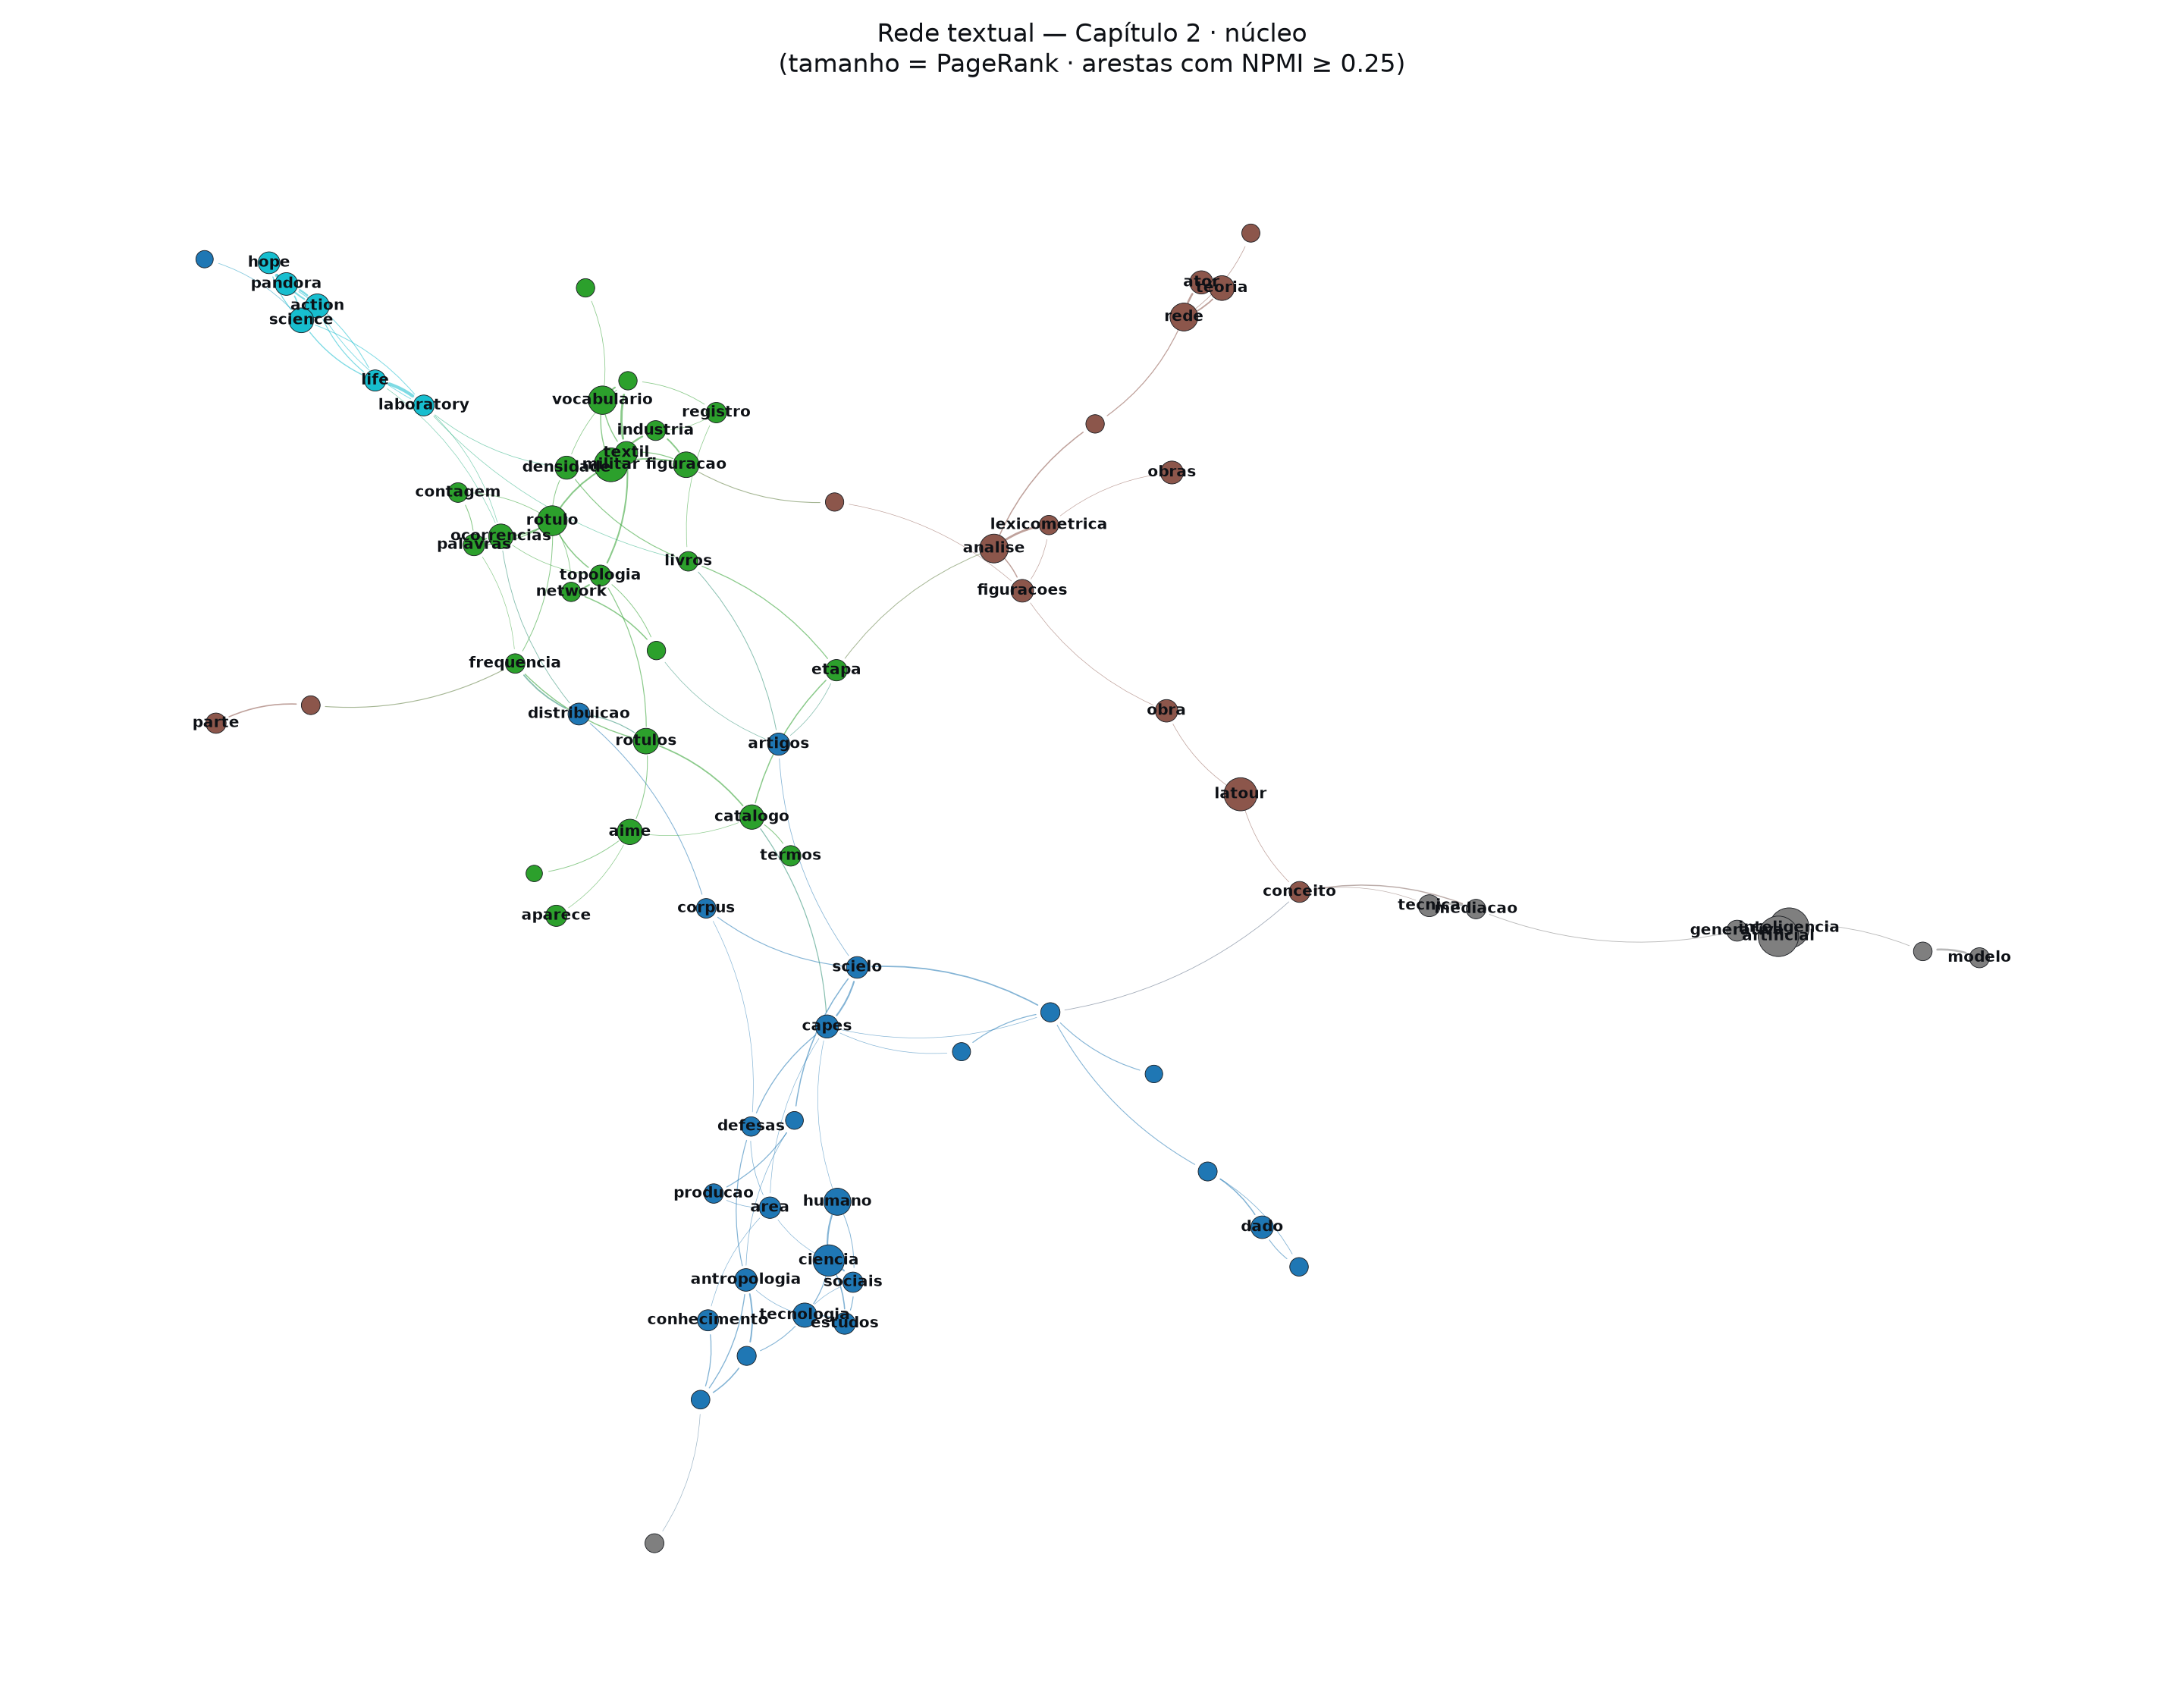
\includegraphics[width=1.0\textwidth,keepaspectratio]{figuras/cap.2/infranodus_cap2_focus_pmi.png}
\caption[Núcleo da rede textual do capítulo~\ref{capitulo2} ponderado por PageRank e NPMI]{Núcleo da rede textual do capítulo~\ref{capitulo2}, ranqueado por critérios informacionais em vez de frequentistas. Os mesmos 100 nós da figura~\ref{fig:infranodus-cap2-focus} são exibidos, mas o tamanho passa a ser proporcional ao \textit{PageRank} (centralidade na rede, em vez de contagem bruta) e as arestas são filtradas pelo \textit{Normalized Pointwise Mutual Information} (NPMI~$\geq 0{,}25$), retendo apenas co-ocorrências surpreendentes dadas as frequências marginais de cada termo. A cor mantém a comunidade Louvain, e as arestas, arqueadas, recebem a mistura das cores das comunidades que ligam. Esta vista promove conceitos pouco frequentes e estrategicamente posicionados, e deprime termos onipresentes cuja associação com qualquer outro é trivial, funcionando como contraponto à leitura puramente frequentista. Métricas e arquivo \texttt{.gexf} no repositório \url{https://github.com/julianehelanski/tecno-etnografia-centro-ia}.}
\label{fig:infranodus-cap2-pmi}
\end{figure}

\begin{figure}[H]
\centering
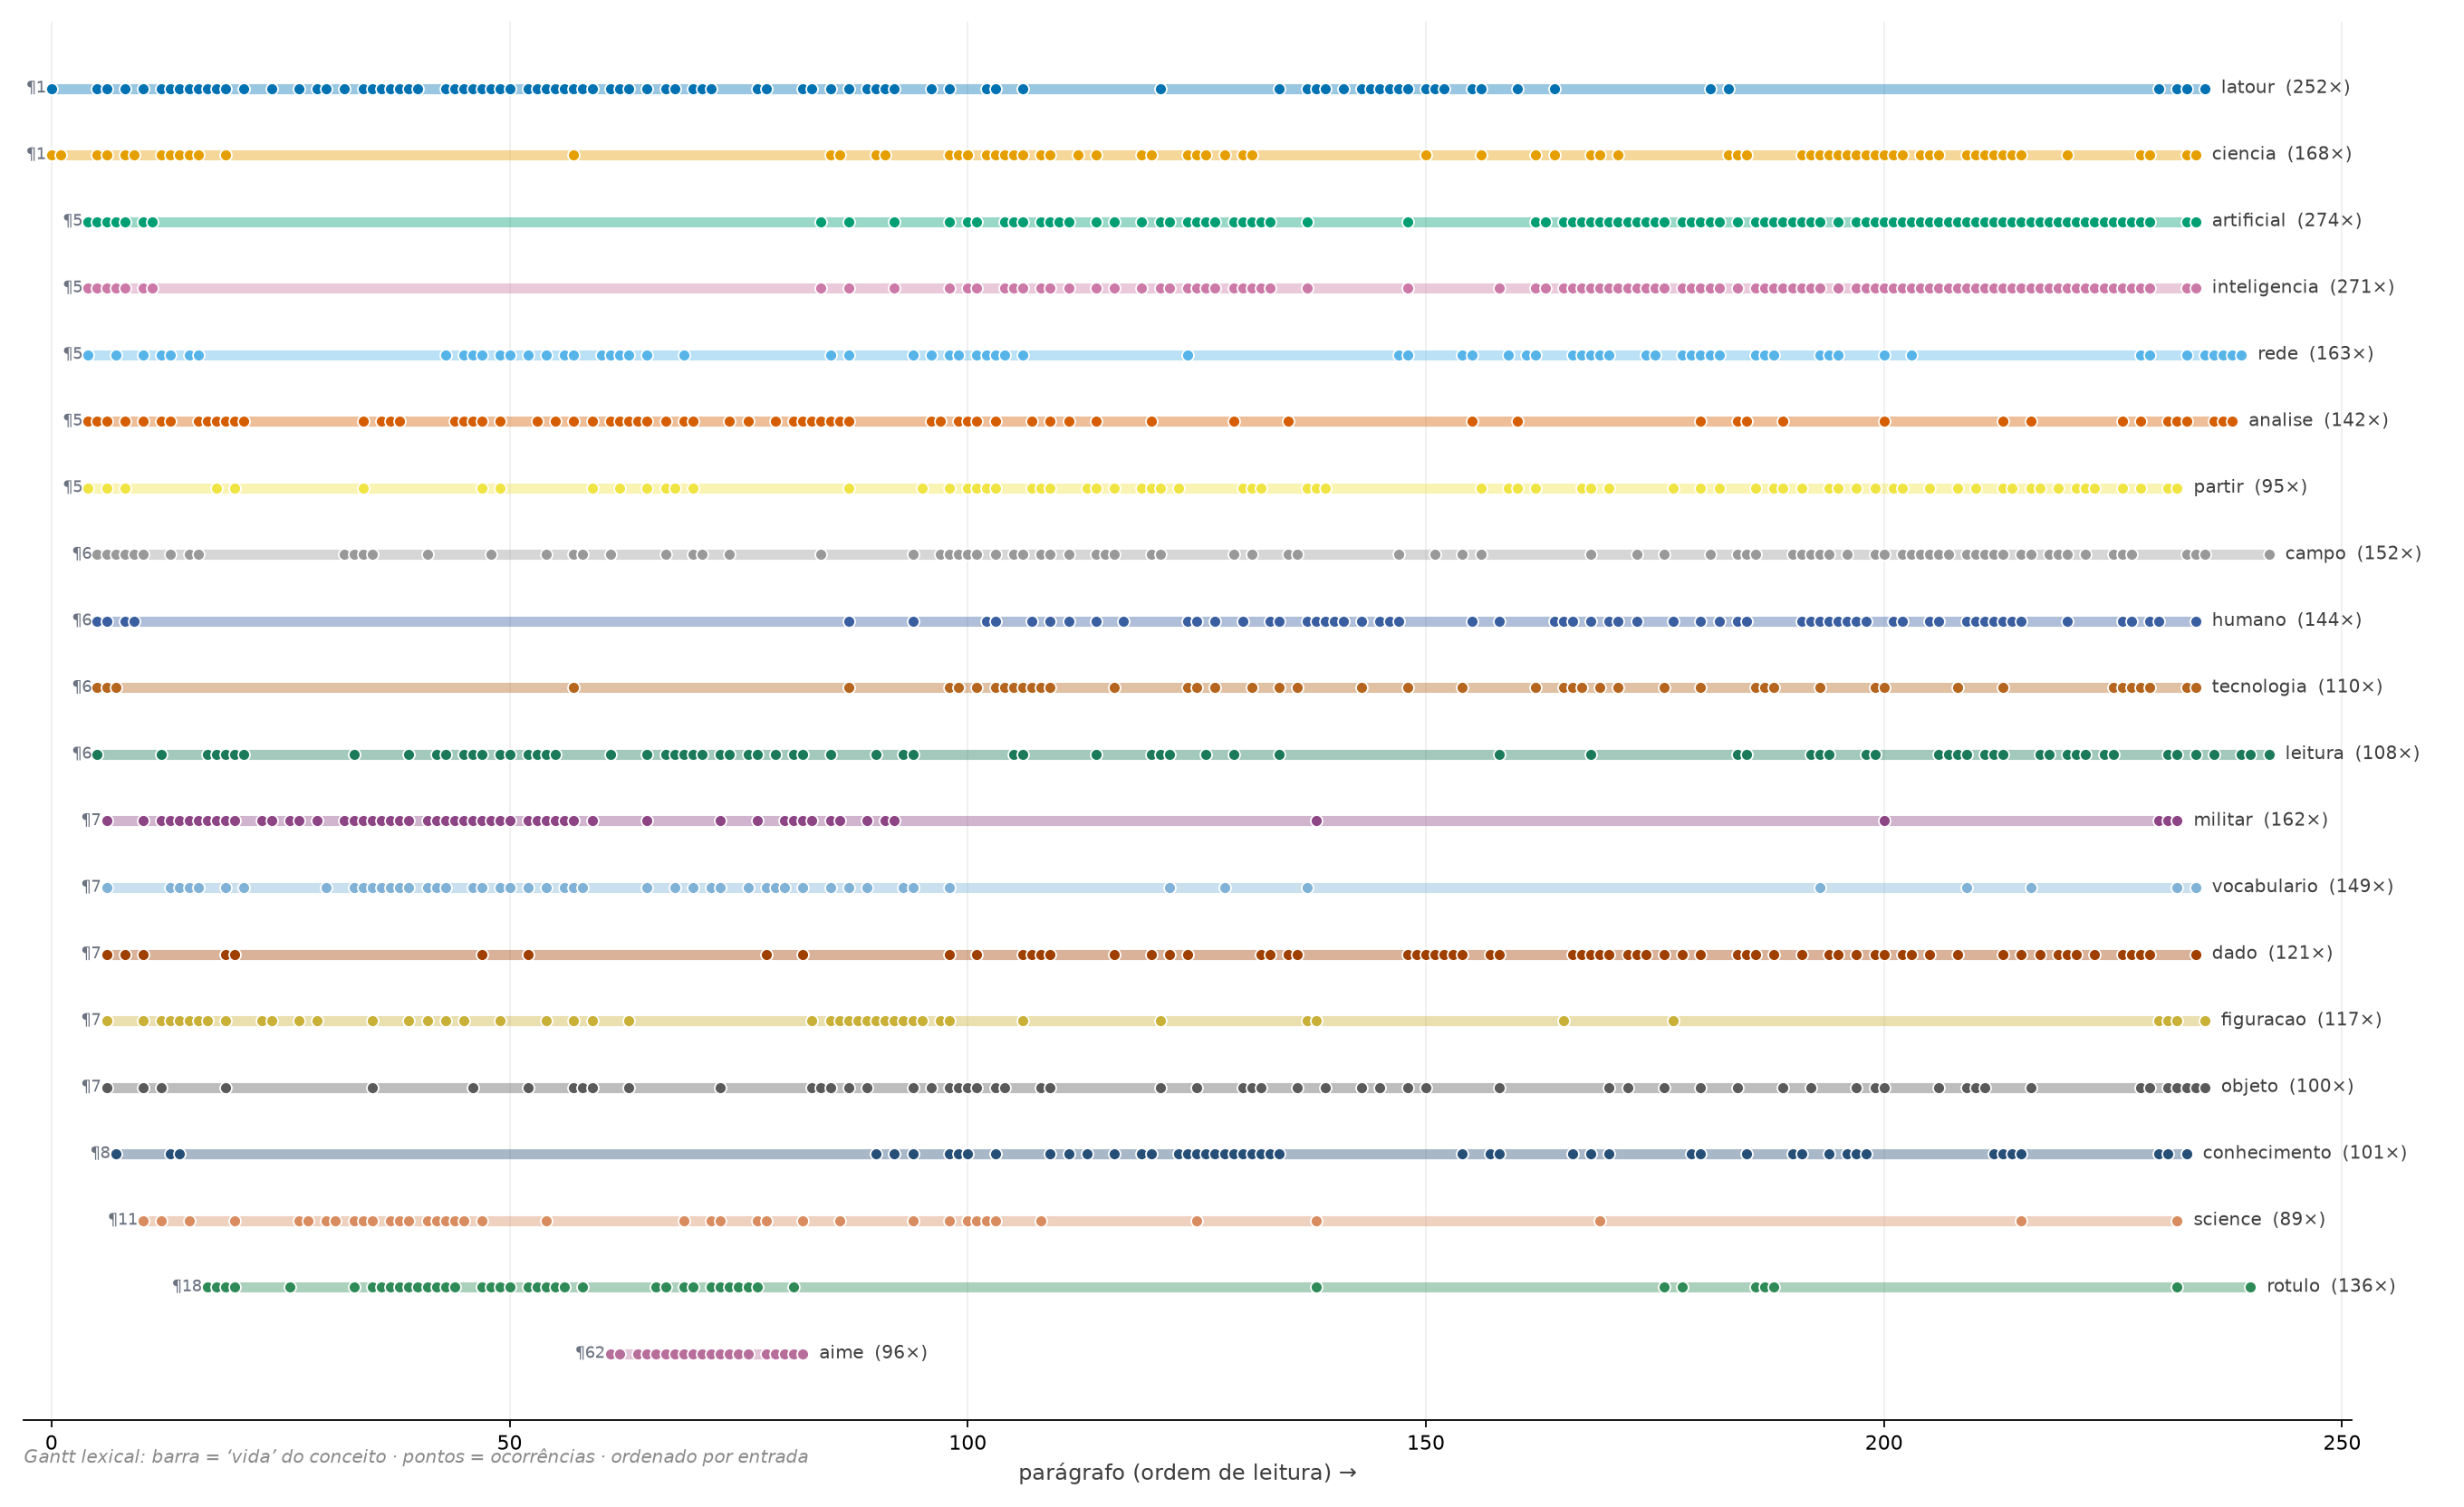
\includegraphics[width=1.0\textwidth,keepaspectratio]{figuras/cap.2/trajectory_gantt.png}
\caption[Gantt lexical do capítulo~\ref{capitulo2}: entrada, persistência e saída dos conceitos]{Gantt lexical do capítulo~\ref{capitulo2}. Cada linha corresponde a um dos 20 conceitos de maior frequência, excluídos termos genéricos e o marcador \texttt{claude}; o eixo horizontal é a ordem de leitura em parágrafos. A barra colorida marca a vida do conceito no capítulo, do parágrafo de primeira aparição (rótulo \P\textit{n}) ao último; os pontos sobre a barra indicam cada ocorrência; o número entre parênteses à direita é a contagem total. As linhas estão ordenadas por parágrafo de entrada, evidenciando a sequência em que cada noção é convocada e por quanto tempo permanece em circulação. Gerado pelo \textit{script} \texttt{narrative\_trajectory.py}, disponível em \url{https://github.com/julianehelanski/tecno-etnografia-centro-ia/tree/main/infranodus}.}
\label{fig:trajectory-cap2-gantt}
\end{figure}

\begin{figure}[H]
\centering
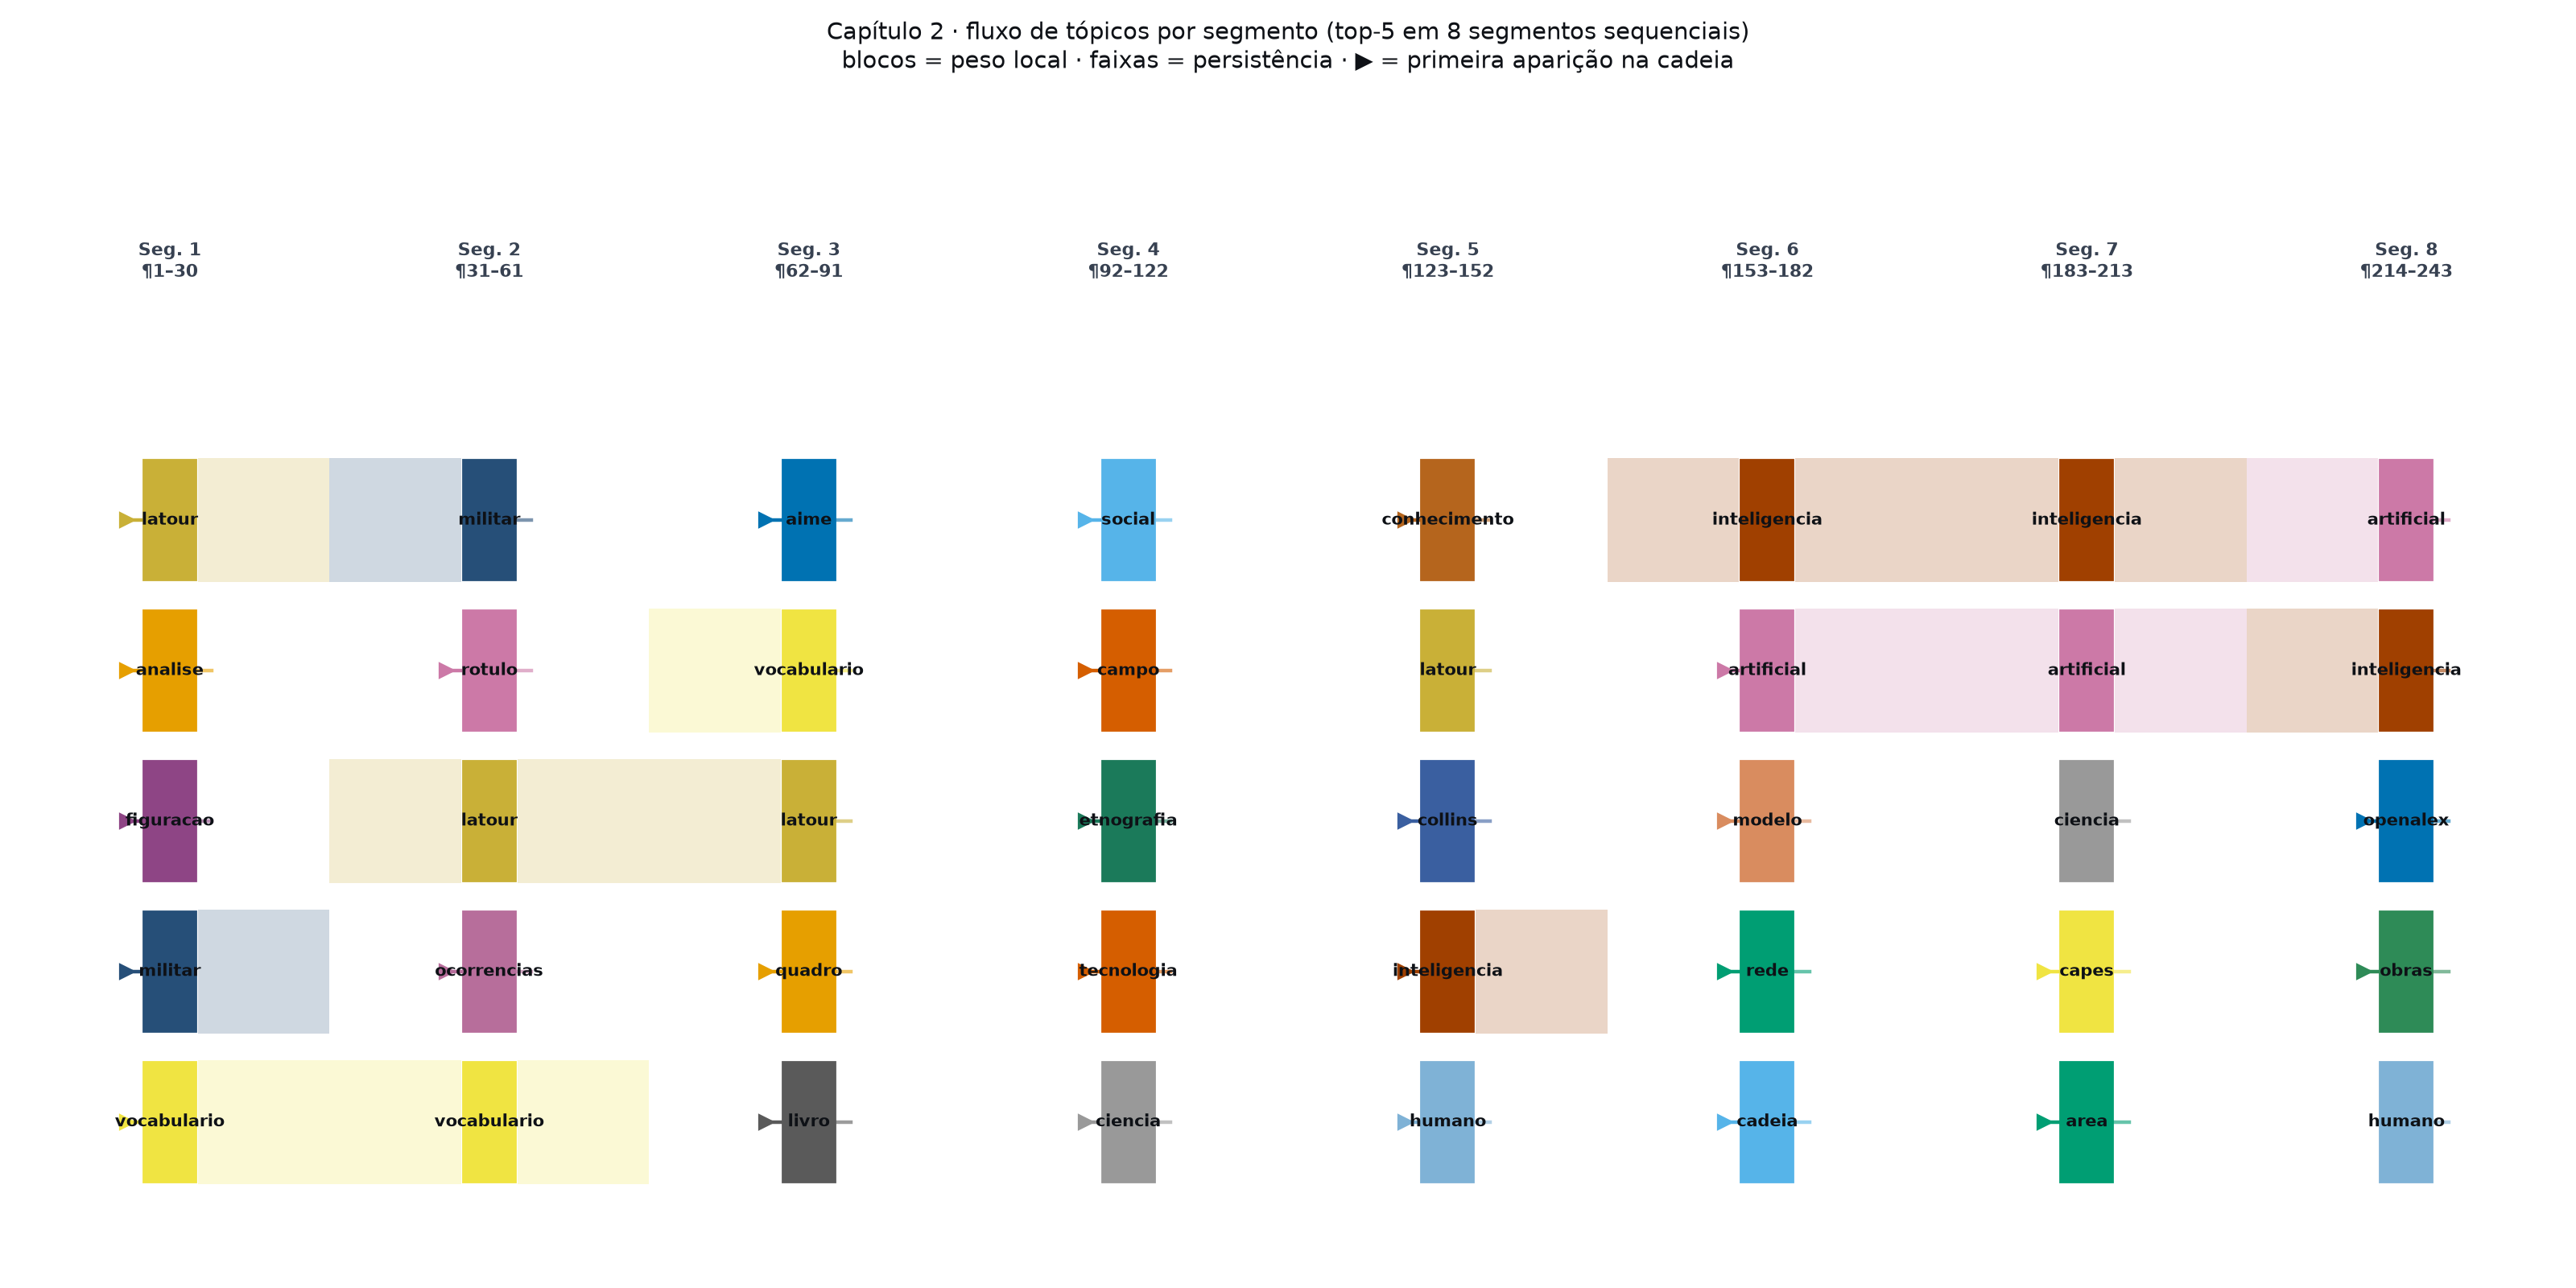
\includegraphics[width=1.0\textwidth,keepaspectratio]{figuras/cap.2/trajectory_alluvial.png}
\caption[Fluxo aluvial de tópicos ao longo do capítulo~\ref{capitulo2}]{Fluxo aluvial do capítulo~\ref{capitulo2}. O capítulo é particionado em 8 segmentos sequenciais de igual extensão em parágrafos (rótulos \P\textit{n}--\P\textit{m} no topo); em cada segmento são listados os 5 termos de maior frequência local (blocos coloridos, com a posição vertical refletindo o \textit{ranking} dentro do segmento). Faixas translúcidas conectam um termo a si mesmo entre segmentos adjacentes quando ele persiste no \textit{top}-5, materializando continuidades temáticas; setas $\blacktriangleright$ assinalam a primeira aparição de um conceito na cadeia. A figura responde à pergunta \enquote{o que se liga a quê ao longo do capítulo} e torna visíveis tanto os tópicos persistentes quanto as entradas tardias e saídas precoces. Gerado pelo \textit{script} \texttt{narrative\_trajectory.py}, disponível em \url{https://github.com/julianehelanski/tecno-etnografia-centro-ia/tree/main/infranodus}.}
\label{fig:trajectory-cap2-alluvial}
\end{figure}

\begin{figure}[H]
\centering
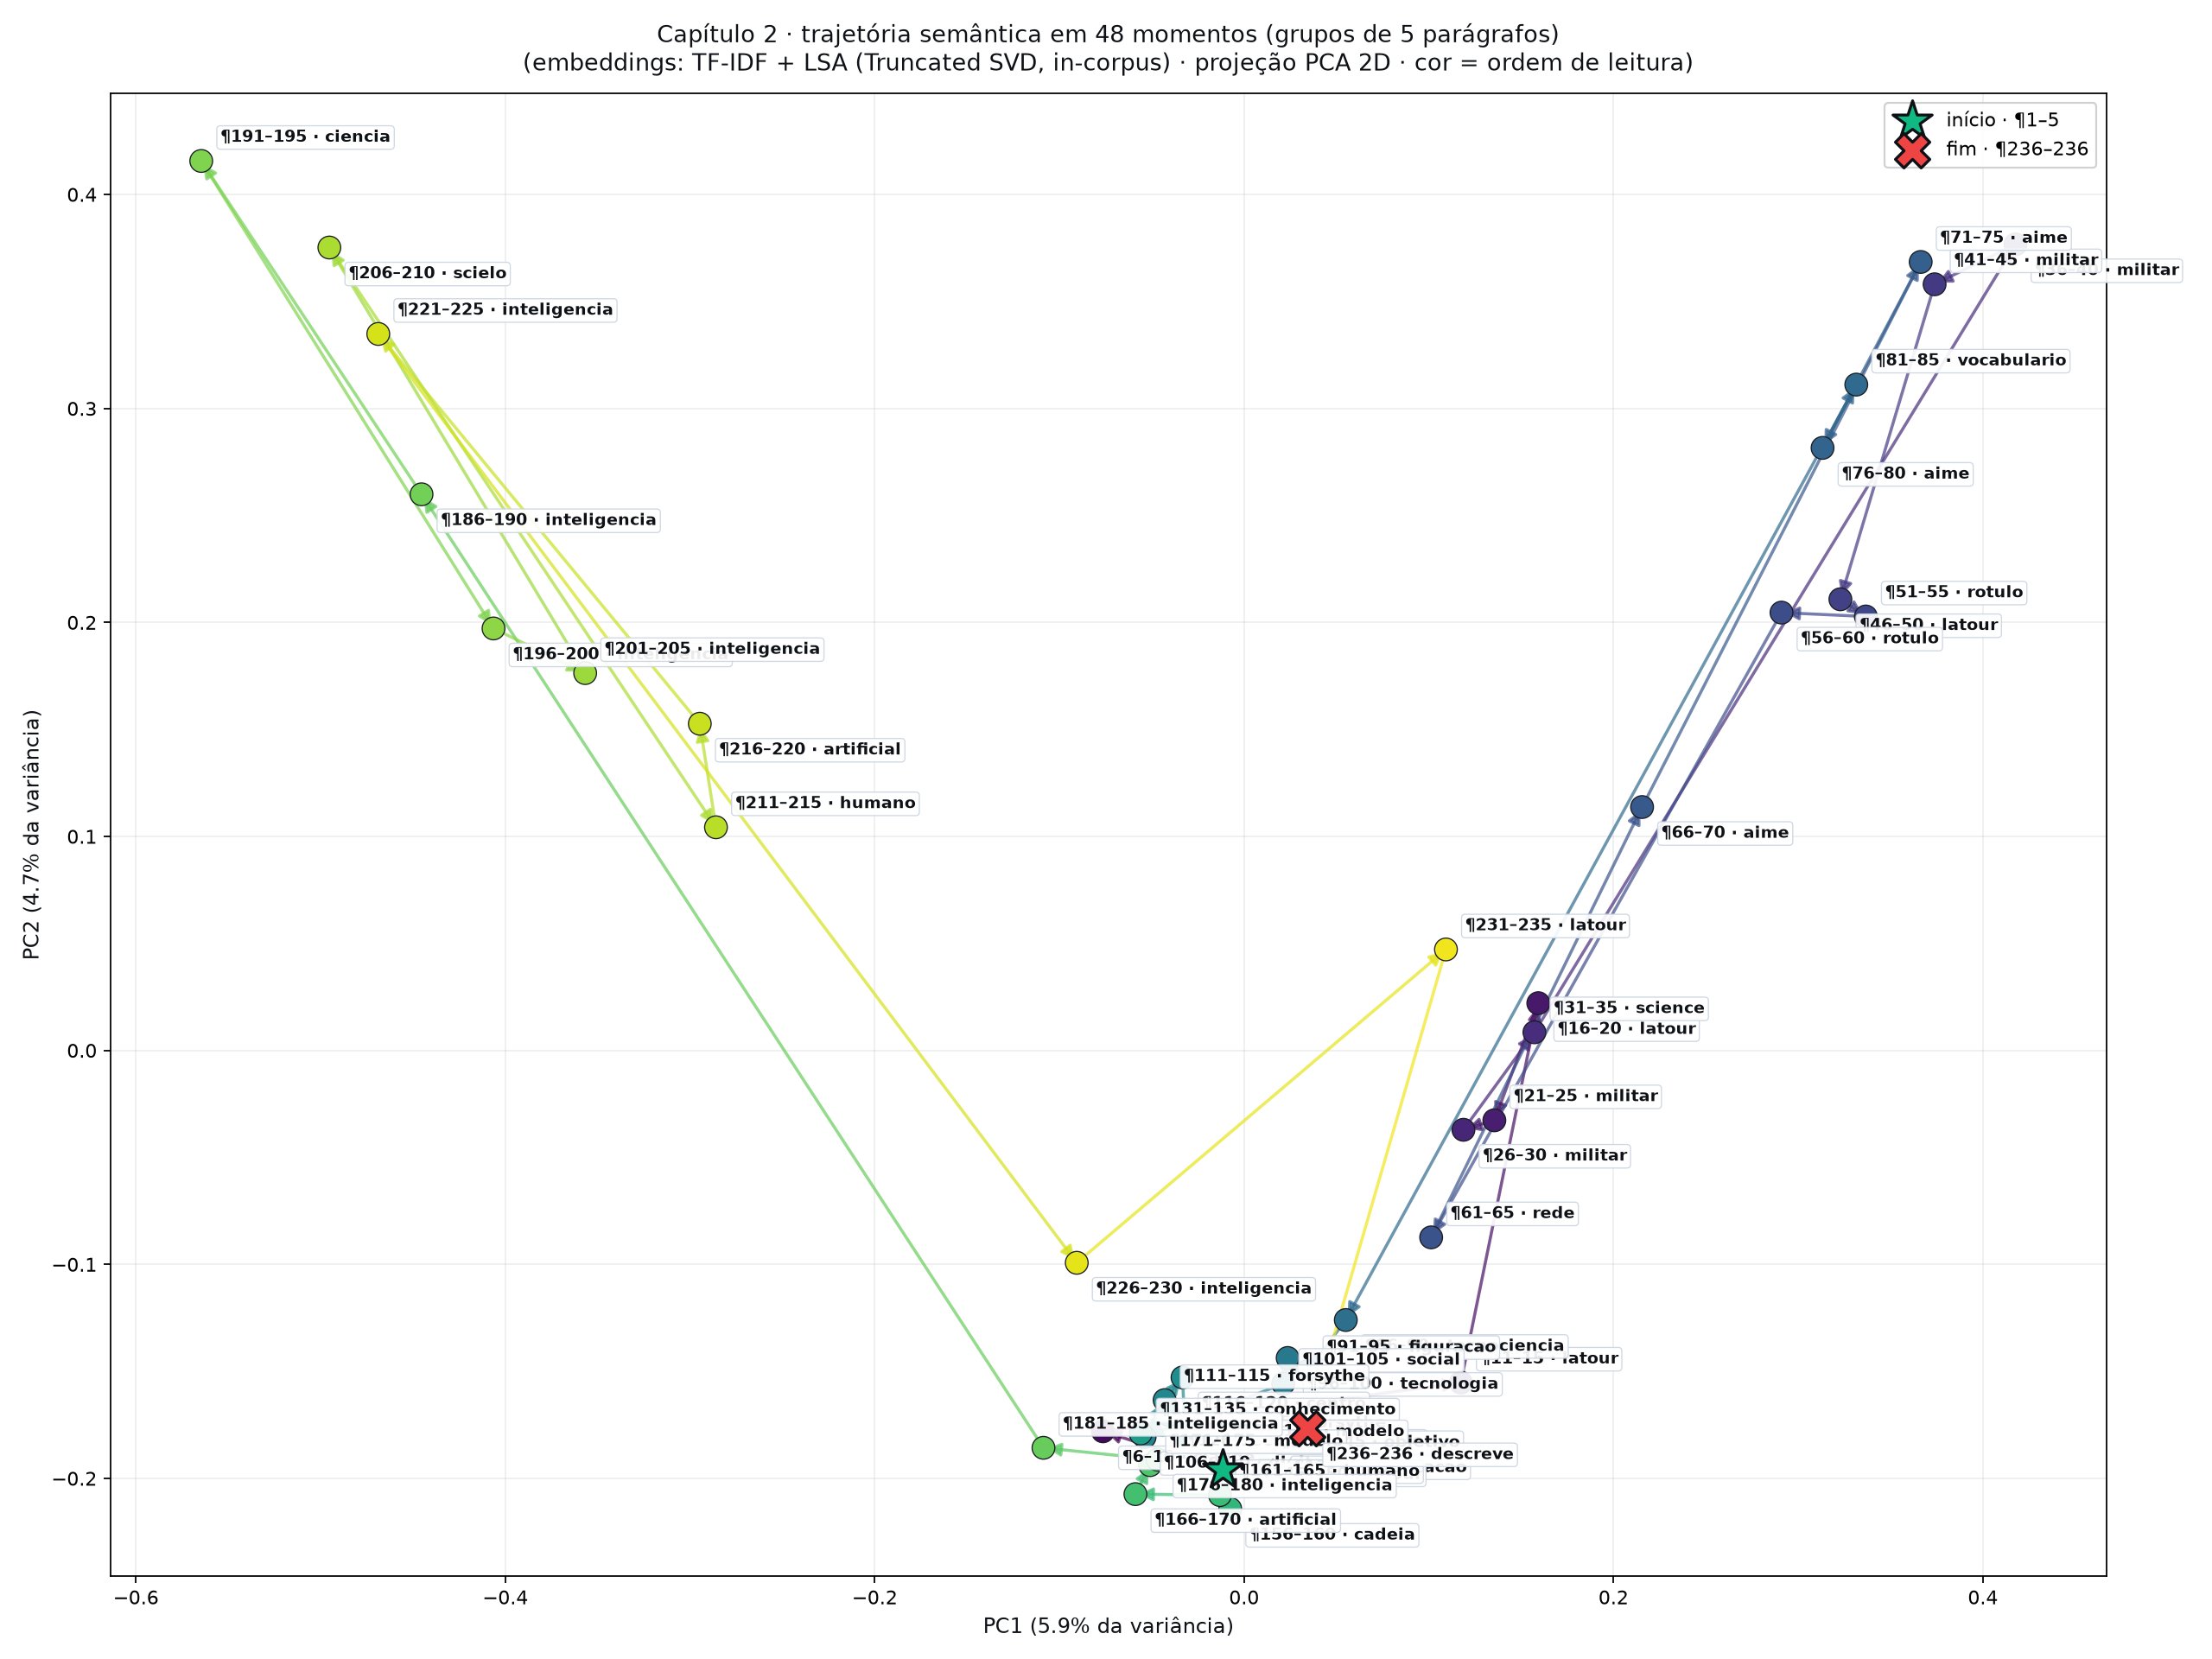
\includegraphics[width=1.0\textwidth,keepaspectratio]{figuras/cap.2/trajectory_semantic.png}
\caption[Trajetória semântica do capítulo~\ref{capitulo2}]{Trajetória semântica do capítulo~\ref{capitulo2}. Os parágrafos são agrupados em \textit{momentos} de 5 parágrafos consecutivos; cada momento é vetorizado por \textit{TF-IDF} (unigramas e bigramas) seguido de redução por \textit{Truncated SVD} (\textit{Latent Semantic Analysis} \textit{in-corpus}, \textit{fallback} usado quando o \textit{sentence-transformer} multilíngue não está disponível) e projetado em duas dimensões por PCA. Cada ponto é um momento, rotulado com o intervalo de parágrafos e o termo dominante; as setas seguem a ordem de leitura, com gradiente \textit{viridis} do início ($\star$ verde) ao fim ($\times$ vermelho). Distâncias no plano aproximam dissimilaridade lexical entre momentos; deslocamentos longos indicam mudanças temáticas, voltas curtas indicam retomada de campo semântico já visitado. O percentual de variância explicada por cada eixo aparece nos rótulos. Gerado pelo \textit{script} \texttt{narrative\_trajectory.py}, disponível em \url{https://github.com/julianehelanski/tecno-etnografia-centro-ia/tree/main/infranodus}.}
\label{fig:trajectory-cap2-semantic}
\end{figure}
\chapter{A rede que Fábio e Cláudio construíram}
\label{capitulo3}

\epigrafe{%
Terceiro princípio: Nunca somos postos diante da ciência, da tecnologia e da sociedade, mas sim diante de uma gama de associações mais fracas e mais fortes, portanto, entender o que são fatos e máquinas é o mesmo que entender o que as pessoas são.}%
{Bruno Latour, \textit{Ciência em ação: como seguir cientistas e engenheiros sociedade afora}, 2011, p.~409}

Este capítulo é uma das quatro tramas da tecnoetnografia que desenvolvo nesta tese, o conceito que apresentei no capítulo~\ref{capitulo1} para nomear a indissociabilidade entre a escrita, a análise e as técnicas com que faço esta pesquisa sobre e com inteligência artificial. Se no capítulo~\ref{capitulo1} a tecnoetnografia se fez como gesto recursivo sobre a descrição etnográfica da tecnociência e seus limites, aqui ela se faz ao seguir as associações de Fábio e de Cláudio até as corporações, os contratos, as políticas de inovação e a trajetória da própria \texttt{IBM}, que recua mais de um século. Seguir essas associações é o que me impede de tomar a ciência, a tecnologia e a sociedade como três domínios já dados, postos diante de mim como blocos a relacionar; o que encontro no campo, e o que descrevo, é uma \enquote{gama de associações mais fracas e mais fortes}, em que descrever o que os contratos, as infraestruturas e as máquinas de Hollerith são não se separa de descrever o que vêm a ser os atores que se associam a eles, pois uns e outros só ganham seus contornos na trama dessas associações. A rede que descrevo neste capítulo, a dos contratos, das infraestruturas, das políticas de fomento e da trajetória corporativa, é a mesma rede sociotécnica que o capítulo~\ref{capitulo4} deixará recuar ao \textit{hinterland}, no sentido de \textcite[pp.~34--42]{Law2004After}, quando a atenção se voltar para as práticas situadas de Marcelo em torno do \texttt{Spira}, sem que essa rede de fundo desapareça, pois ela continua sendo condição de possibilidade do que aparece em primeiro plano. O que distingue este capítulo do capítulo~\ref{capitulo4} está no segmento da mesma rede que escolho seguir e no lugar onde decido começar e parar: aqui acompanho uma cadeia que se estende por muitos nós e por mais de um século; lá, Marcelo me levará a um segmento curto, em que as associações se atam mais intensamente umas às outras. Nenhum dos dois segmentos é maior ou menor que o outro, apenas mais ou menos longo, mais ou menos intensamente conectado, na formulação de \textcite{latour1996clarifications} que retomei do capítulo~\ref{capitulo1}, e o corte que decide por onde a rede se deixa rastrear é o que a faz existir como objeto etnográfico, no sentido que tomei de Strathern \parencite{strathern2011cortando}.\footnote{Latour formula a recusa das separações herdadas em dois registros que retomo ao longo deste capítulo. Na epígrafe, retirada de \textcite[p.~409]{Latour2011CienciaEmAcao}, o terceiro princípio recusa a tripartição entre ciência, tecnologia e sociedade e sustenta que só há uma gama de associações mais fracas e mais fortes, de modo que entender o que são os fatos e as máquinas se confunde com entender o que vêm a ser as pessoas. No texto sobre as propriedades da rede, Latour recusa as três dimensões espaciais herdadas das ciências sociais, a escala (grande e pequeno), a distância (perto e longe) e o limite (dentro e fora), e mostra que uma rede nunca é maior que outra, apenas mais longa ou mais intensamente conectada \parencite{latour1996clarifications}. Os dois registros convergem na mesma tese: a força e a fraqueza, o comprimento e a intensidade da conexão são graus de um único contínuo de associações, e não propriedades de domínios ou de escalas distintas. É por isso que a diferença entre este capítulo e o capítulo~\ref{capitulo4} se decide no corte que faço sobre a mesma rede, no sentido de \textcite{strathern2011cortando}, e não em uma diferença de natureza entre duas redes.}

Segui Fábio e Cláudio presencialmente, ao longo dos eventos, das conversas e das reuniões em que os encontrei, durante aproximadamente quatro anos de pesquisa etnográfica (2022--2025) no \texttt{C4AI}. O trabalho de campo intensificou-se a partir de fevereiro de 2023, quando assisti à \textit{bluetalks} (encontro corporativo para discutir tecnologia e inovação) realizada no Inovabra Habitat em São Paulo,\footnote{O Inovabra é um espaço de inovação criado pelo banco Bradesco, situado na região da Avenida Paulista, em São Paulo, que aproxima \textit{startups}, empresas, mentores e investidores. O evento ocorreu poucos meses antes de a Organização Mundial da Saúde declarar, em maio de 2023, o fim da emergência de saúde pública internacional da Covid-19.} evento em torno do qual se organizou a problematização que deu origem a este capítulo. Numa quinta-feira de fevereiro, eu era parte da audiência quando uma pessoa da plateia, uma mulher cujo nome não registrei, perguntou a Cláudio, vice-diretor do \texttt{C4AI} e à época ainda pesquisador da \texttt{IBM}, o que a \texttt{IBM} ganhava com o investimento no centro. Cláudio respondeu que a empresa se beneficiava ao \enquote{incentivar um ecossistema de inovação em inteligência artificial} para que as pesquisas atendessem às necessidades do setor, de modo que surgiria \enquote{uma demanda por serviços que a IBM poderia fornecer}. Foi essa resposta, dada naquelas condições, que me deteve. Embora circule amplamente a percepção de que empresas buscam extrair valor de suas parcerias, poucas vezes se descreve o que de fato circula nessas cadeias, por quais caminhos e sob que termos, e foi essa a lacuna que tomei como questão. Não tomo a resposta de Cláudio como descrição verificada do que a \texttt{IBM} ganha, e não disponho de meios para saber se o retorno que ele antecipava chegou a se confirmar; o encerramento posterior da operação da empresa no Brasil, que ultrapassa o \texttt{C4AI} e ao qual retorno ao fim deste capítulo, deixa a questão em aberto. A fala abriu a pergunta que eu viria a perseguir, a de como circula o valor nessas cadeias, e foi ao perseguir o que ela significava que entendi o que era seguir Fábio e Cláudio: acompanhar as associações que eles faziam e, ao mesmo tempo, fazer associações eu própria ao segui-los, de modo que eu também entrava na rede que descrevia.

Foi também assim que cheguei à \texttt{IBM} como objeto de pesquisa. Até então, a empresa era um ator coadjuvante que ora aparecia, ora recuava, e como investigar o convênio público-privado em si não estava entre minhas intenções, eu nunca lhe havia dado a atenção que ela merecia. Ao perseguir o que a resposta de Cláudio significava, a \texttt{IBM} deixou de ser figura de fundo e passou a ocupar o centro desta investigação, num deslocamento metodológico que mudou o foco de uma etnografia do presente, de como se faz pesquisa em IA no \texttt{C4AI}, para uma investigação histórica que relaciona este centro a práticas tecnocientíficas estabilizadas pela \texttt{IBM} ao longo de mais de um século. Tomá-la como objeto e levar essa análise adiante tensionou a minha posição de pesquisadora, e foi por meio dela que experimentei, na própria prática, o esforço de fazer alianças sem ferir os sentimentos estabelecidos, no sentido de Stengers, que abordei no capítulo~\ref{capitulo1}. Como viria a descobrir, esta etnografia tornou-se também um registro, ou uma reconstrução, da trajetória do acordo \texttt{C4AI-IBM-FAPESP}, desde a sua criação em 2020, passando por sua relativa consolidação e multiplicação institucional, até o seu encerramento pela \texttt{IBM} em dezembro de 2025. O que começou como tentativa de compreender como se faz IA em um centro de pesquisa transformou-se, por força do próprio campo, em documentação de como arranjos desse tipo se formam, funcionam e acabam, e de como relações de poder, o \textit{tecnopoder} que proponho nomear adiante, mostram-se em momentos de tensão, de crise e de êxito, revelando negociações nem sempre explícitas entre atores e actantes que transitam entre discursos sobre \enquote{IA responsável}, \enquote{bem social} e \enquote{mercado}. Essas racionalidades corporativas continuam a influenciar relações entre corporações globais e instituições acadêmicas que, embora robustas em seus contextos nacionais, ocupam posição periférica nos ecossistemas globais de inovação em inteligência artificial, ecossistemas que influenciam, e até mesmo determinam, quem pode fazer IA, como fazer, para quê e para quem.

À fala da \textit{bluetalks} soma-se uma segunda, que Cláudio me deu em entrevista realizada em 2025, e os dois são fios distintos que costuro ao longo desta trama: o primeiro diz respeito ao que a \texttt{IBM} ganha ao cultivar um ecossistema de pesquisa em torno de si, e o segundo, ao modelo de negócio que a empresa montou sobre o código aberto. Aproximá-los não os torna a mesma coisa, e é a relação entre eles que a investigação histórica deste capítulo procura descrever. Referindo-se a esse modelo de negócio, Cláudio mencionou que a \texttt{IBM} \enquote{descobriu na década de 90} como fazer dinheiro com \texttt{Linux} e sistemas abertos (\textit{open source}). Chamou-me a atenção a escolha do verbo: \enquote{descobriu}, e não \enquote{desenvolveu} ou \enquote{inventou}. Leio nessa escolha um indício de que se trata, para ele, de uma prática que a \texttt{IBM} encontrou já formada e passou a explorar, em lugar de algo que ela teria criado, e é essa leitura que a investigação histórica deste capítulo desenvolve.

Foi seguir o que \textit{descobriu} implicava que me levou a investigar o que o código aberto tinha a ver com o \texttt{C4AI} e com os ecossistemas de inovação em IA. O paralelo com a inteligência artificial contemporânea é de longa duração: assim como o modelo de negócios de código aberto permitiu que corporações extraíssem valor gerado coletivamente por comunidades de desenvolvedores, os atuais modelos de IA dependem da extração e do processamento de conhecimento produzido coletivamente, seja por meio de dados gerados por usuários, cuja origem se torna difícil de rastrear na escala em que esses sistemas funcionam,\footnote{Se o caso do \texttt{GitHub Copilot} expõe o corte da propriedade no plano do código, os dados de treinamento o expõem em outra escala. A auditoria de \textcite{Longpre2024Provenance} sobre quase quatro mil conjuntos de dados públicos de texto, fala e vídeo, produzidos entre 1990 e 2024, precisou rastrear manualmente cada conjunto até suas fontes originais, percorrendo cadeias de repositórios, sites e artigos, porque a documentação de proveniência se perde a cada vez que um conjunto é reempacotado e re-licenciado. Os autores constatam que, embora menos de um terço dos conjuntos tenha licença restritiva, mais de 80\% do conteúdo de suas fontes carrega restrições não declaradas na licença final, e que a licença do conjunto contradiz os termos da fonte em mais da metade do conteúdo de texto. O rastreamento foi possível para os auditores, ao custo de um trabalho manual extenso, mas não está documentado para quem usa esses conjuntos nem para quem teve seus dados incorporados a eles: a origem é conhecida por quem coleta e se apaga para quem contribuiu. A irrastreabilidade, no caso da IA, distribui-se de modo desigual entre os lados da rede.} seja pelos vínculos com universidades públicas que fornecem pesquisadores, infraestrutura e legitimidade epistêmica.\footnote{Desenvolvo essa literatura crítica da extração algorítmica e da inteligência artificial no capítulo~\ref{capitulo2} (seção~\ref{sec:predicao_poder}), a propósito de Kate Crawford, Vladan Joler e Matteo Pasquinelli: as cartografias que seguem as cadeias materiais, laborais e epistêmicas da IA, e o argumento de que esses sistemas atualizam padrões de longa duração de colonialismo e extração.} O caso do \texttt{Linux} evidencia, historicamente, a apropriação corporativa do conhecimento coletivo na indústria de tecnologia. Trata-se de um modelo que funciona simultaneamente em dois registros: produz bens públicos (código aberto, modelos de IA, publicações científicas) enquanto gera lucro privado (serviços, consultorias, infraestrutura proprietária). Bem público, porém, não é o mesmo que bem social: um sistema de IA pode ser tecnicamente \enquote{aberto} e ainda assim aprofundar desigualdades e favorecer infraestruturas proprietárias. Os recursos que utilizei para as análises computacionais desta tese são um exemplo de como isso funciona na prática: hospedo no \texttt{GitHub} os repositórios públicos desta pesquisa, da análise lexicométrica ao código-fonte do texto. A mesma abertura que torna o meu trabalho verificável, auditável e reexecutável o disponibiliza como código público a quem treina modelos sobre esses acervos.\footnote{A \texttt{Microsoft} comprou o \texttt{GitHub}, plataforma que hospeda boa parte do desenvolvimento de código aberto do mundo, em 2018, por US\$ 7,5 bilhões \parencite{Microsoft2018GitHub}; em 2021, o \texttt{GitHub Copilot}, assistente de programação movido pelo modelo \texttt{Codex} da \texttt{OpenAI}, foi lançado treinado sobre bilhões de linhas de código público hospedado na própria plataforma, sem a atribuição de autoria que as licenças \textit{open source} exigem, o que motivou uma ação coletiva contra \texttt{GitHub}, \texttt{Microsoft} e \texttt{OpenAI} em 2022.}

O termo \textit{tecnopoder} deriva da noção de \enquote{poder artificial} (\textit{Artificial Power}) com que \textcite{Brennan2025ArtificialPower} sintetizam o contexto em que uma \enquote{oligarquia tecnológica} mobiliza a IA, como uma categoria de marketing e como conjunto de tecnologias de automação, para consolidar e ampliar o seu poder. Tomo esse termo emprestado e o desloco para o meu material, para investigar práticas tecnocientíficas da \texttt{IBM} ao longo de 135 anos, dos cartões perfurados de Hollerith às plataformas de IA contemporâneas. A derivação é também conceitual: o que muda é o estatuto que cada abordagem confere à desigualdade de poder. Para a literatura crítica das \textit{big techs}, que pensa a IA como concentração de poder, essa desigualdade é o que explica os arranjos concretos; para a teoria ator-rede que sigo, ela é o efeito que precisa ser descrito, rastreado associação por associação até os mecanismos que o produzem, e não a causa que explica. Mantenho as duas formas de investigação em tensão: recorro à teoria ator-rede para descrever como as desigualdades se fazem, relação por relação, e ao vocabulário da crítica para nomear o padrão histórico desse contexto, ciente de que esse vocabulário, com termos como captura, dependência e extração, carrega pressupostos sobre estruturas tecnocientíficas geralmente problemáticos para o escopo da teoria ator-rede. É dessa tensão que extraio o método: a descrição actante a actante me impede de tomar a desigualdade como causa já pronta, e o vocabulário da crítica me impede de dissolver, na simetria descritiva, a desigualdade de poder que o campo me apresentou. É nesse intervalo que situo o \textit{tecnopoder}.

Cheguei à \texttt{IBM}, portanto, seguindo as falas públicas de Fábio e de Cláudio, e a pergunta que alguém da plateia da \textit{bluetalks} dirigiu a Cláudio, e com ela a um sistema de tabulação, a máquina tabuladora que Herman Hollerith (1860--1929) criou nos finais do século XIX. Embora este seja o terceiro capítulo na ordem em que a tese se lê, foi a \texttt{IBM} o primeiro dos sítios que segui a se impor à investigação, e marco essa diferença porque foi seguir os atores que decidiu por onde a pesquisa começaria a se adensar. O lugar que a empresa veio a ocupar na pesquisa contrariou o que eu esperava. Eu entrara em campo determinada a fazer uma etnografia mais voltada aos actantes não humanos, os sistemas de IA do centro, que aos atores, os cientistas e engenheiros, e contava encontrar um laboratório de pesquisa em IA onde observaria de perto como se faz inteligência artificial. O laboratório que eu imaginava não estava lá. Foi a frustração dessa expectativa, que no capítulo~\ref{capitulo1} formulei como a pergunta \emph{onde está o laboratório e os seus cientistas?} (seção~\ref{onde-esta-laboratorio-cientistas}), que me levou, primeiro, à \texttt{IBM} e a Hollerith: é aqui, nesta rede, que aquela pergunta que abri no início desta tese ganhou contornos próprios. O conselho de Latour para suspender preconceitos e expectativas ao entrar no mundo da ciência e da tecnologia valeu-se nesse ponto, quando a expectativa frustrada se tornou uma condição de realização desta etnografia.\footnote{\enquote{O equipamento necessário para viajar pela ciência e pela tecnologia é, ao mesmo tempo, leve e variado. Variado porque é preciso misturar pontes de hidrogênio com prazos finais, exame da capacidade alheia com dinheiro, correção de sistemas de computadores com estilo burocrático; mas o equipamento também é leve porque convém deixar de lado todos os preconceitos sobre as distinções entre o contexto em que o saber está inserido e o próprio saber. Na entrada do inferno de Dante está escrito: DEIXAI A ESPERANÇA, Ó VÓS QUE ENTRAIS. No ponto de partida desta viagem deveria estar escrito: DEIXAI O SABER SOBRE O SABER, Ó VÓS QUE ENTRAIS.}\parencite[p.~10]{Latour2011CienciaEmAcao}.}

\section{Do C4AI-IBM à Terra}
\label{sec:cadeia_translacao}

A Figura~\ref{fig:texto-mapa-cap3} constitui um texto-mapa em que o percurso do capítulo se distribui em uma superfície cuja leitura faço em etapas: parto da pergunta que o campo me deu, sigo pelos fios que dela se desdobram até as máquinas de Hollerith, e chego, por fim, ao arremate que reabre a questão sobre a universidade. O capítulo inicia com a decisão de seguir Fábio e Cláudio, abre a pergunta histórica sobre o ecossistema de inovação, reconstrói a trajetória da \texttt{IBM} de Hollerith ao \texttt{C4AI}, mostra o que as entrevistas tornaram dizível, incluindo a análise bibliométrica das publicações do centro, e lê o fim da parceria como o evento que torna legíveis as ausências que o arranjo não inscreveu, para então devolver, nas considerações finais, a pergunta sobre o lugar da universidade na pesquisa em IA.

\begin{figure}[!htb]
  \centering
  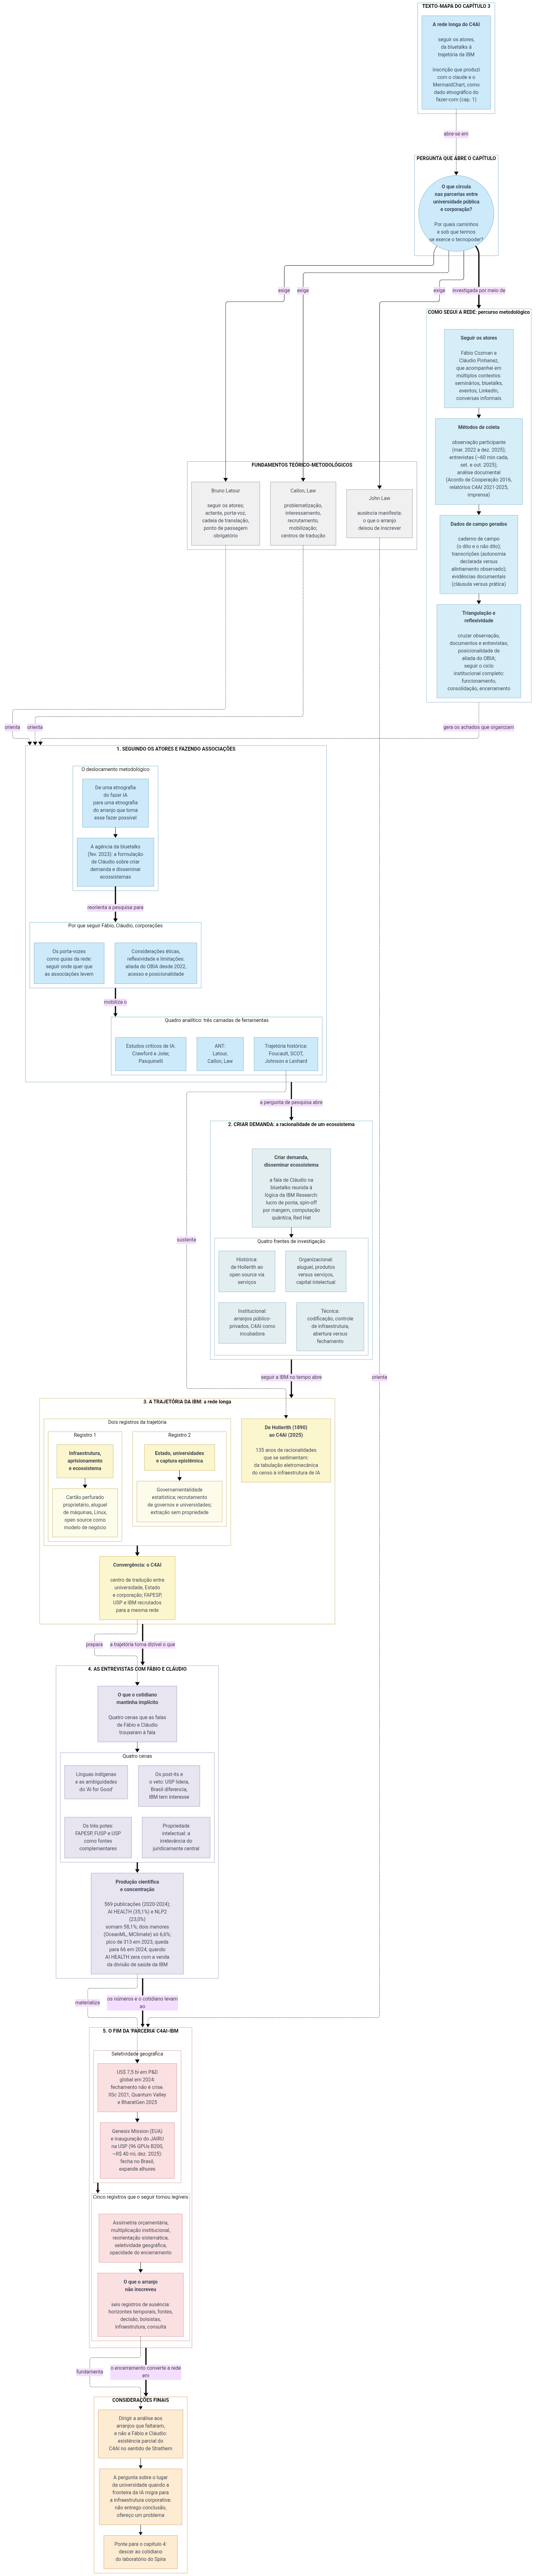
\includegraphics[width=0.2\textwidth,keepaspectratio]{figuras/cap.3/diagramas/mapa-capitulo3.png}
  \caption[Texto-mapa do capítulo~\ref{capitulo3}]{\textbf{Texto-mapa do capítulo~\ref{capitulo3}: a rede longa do \texttt{C4AI}, dos porta-vozes à trajetória da \texttt{IBM}.} A inscrição dispõe o percurso do capítulo a partir da pergunta que o campo me devolveu, sobre o que circula nas parcerias entre universidade pública e corporação, por quais caminhos e sob que termos se exerce o tecnopoder. Três fundamentos sustentam o percurso: \textcite{Latour2011CienciaEmAcao} (seguir os atores), \textcite{Callon1986Sociology} (problematização, interessamento, recrutamento e mobilização) e \textcite{Law2004After} (a ausência manifesta, o que o arranjo deixou de inscrever). (i)~Em \textit{Do C4AI-IBM à Terra}, parto da pergunta que o campo me devolveu e sigo a cadeia de translação para trás no tempo, da parceria à tabulação de Hollerith e ao \textit{khipu}, e para baixo na matéria, até o mineral e a Terra de que a inteligência artificial nunca se desprende. (ii)~Em \textit{Seguindo Fábio e Cláudio: observação, entrevistas e documentos}, o deslocamento de uma etnografia do fazer IA para uma etnografia do arranjo que torna esse fazer possível, ativado pela agência da \textit{bluetalks} de fevereiro de 2023, mobiliza o mapa analítico em três conjuntos (teoria ator-rede; trajetória histórica com Foucault, a SCOT de Bijker e Pinch e o \textit{momentum} de Hughes; estudos críticos de IA com Crawford, Joler e Pasquinelli). (iii)~Em \textit{\enquote{Criar demanda}: a racionalidade de um ecossistema}, a fala de Cláudio na \textit{bluetalks} reúne-se à lógica da \texttt{IBM} Research e abre as quatro frentes da pergunta histórica, da tabulação ao \textit{open source} via serviços. (iv)~Em \textit{A trajetória da \texttt{IBM}}, a rede longa de Hollerith (1890) ao \texttt{C4AI} desdobra-se em dois registros, a infraestrutura e o aprisionamento por ecossistema e a captura epistêmica do Estado e das universidades, que convergem no \texttt{C4AI} como centro de tradução. (v)~Em \textit{As entrevistas com Fábio e Cláudio}, quatro cenas que o cotidiano mantinha implícitas (o \textit{Design Thinking} e o veto corporativo, os três potes do financiamento, a propriedade intelectual e as ambiguidades do \textit{AI for Good}) levam à análise bibliométrica das publicações do centro. (vi)~Em \textit{O fim da \enquote{parceria} \texttt{C4AI-IBM}}, a seletividade geográfica dos investimentos da \texttt{IBM} e os cinco registros que emergiram do seguir dos atores levam aos seis registros de ausência, o que o arranjo não inscreveu. As considerações finais dirigem a análise aos arranjos que faltaram, devolvem a pergunta sobre o lugar da universidade e fazem a ponte para o capítulo~\ref{capitulo4}. Versão interativa disponível em \url{https://mermaid.ai/d/0c8eb50f-d995-4bba-b60a-c768ebe5dd51}.}
  \label{fig:texto-mapa-cap3}
\end{figure}

Esta investigação, que se intensifica a partir de uma rápida conversa num auditório de banco em São Paulo e recua até a máquina de tabular cartões perfurados de 1890 nos Estados Unidos, foi o que significou, neste capítulo, \enquote{seguir os atores}: seguir o fio da conversa que Fábio e Cláudio iam tecendo quando se referiam a noções como \enquote{ecossistema de inovação} e \enquote{criação de demanda}, ou ao modo como a \texttt{IBM} \enquote{descobriu nos anos 90} a possibilidade de lucrar com código aberto. Associação por associação, surgiam questões que me fizeram voltar ao tempo e perguntar: por quais modos uma corporação passa a extrair valor de suas conexões com universidades? O que significa \enquote{fortalecer um ecossistema de IA}? De que maneira se \enquote{descobre} um modelo de negócios baseado em código aberto, e como essa descoberta passa a orientar políticas tecnocientíficas globais de empresas de alta tecnologia? E como tudo isso se relaciona com um centro de IA em uma universidade pública brasileira? Trago essas perguntas porque foram elas o material que pôs o pensamento em movimento. Algumas se desdobraram na trajetória histórica que reconstruo a seguir, outras permaneceram abertas, e é desse desdobramento que se faz a trama deste capítulo.

Como discuti no capítulo~\ref{capitulo1}, subseção~\ref{subsec:cortando-redes}, seguir cientistas e engenheiros universidade afora implicou atravessar fronteiras disciplinares, temporais e geográficas e, sobretudo, manter-me \enquote{tão indecisa quanto os diversos atores que seguia}, ou seja, retomando a epígrafe que abre este capítulo, resistir à tendência de separar o \enquote{técnico} do \enquote{social}, o \enquote{interno} do \enquote{externo}, o \enquote{científico} do \enquote{comercial}. A escolha de quem seguir, porém, foi decidida. Comecei por Fábio e Cláudio porque eram quem mais se sobressaía no campo naquele momento da pesquisa, falando do centro em toda parte, à frente de um arranjo em consolidação e em busca de aliados, e foi a essa proeminência que respondi quando os escolhi como atores a seguir, na seleção das entrevistas que descrevo no capítulo~\ref{capitulo1}, subseção~\ref{subsec:corte_reflexivo_cap1}. Que eles falavam em nome do \texttt{C4AI}, eu viria a descrevê-los como porta-vozes, no sentido que assento adiante; no instante da escolha, porém, o que se impôs foi essa presença proeminente. Os caminhos que essa escolha abriu, fui-os fazendo conforme as associações se desenrolavam, de modo que eu não dispunha, de antemão, de onde a rede que eles construíam começava nem de onde eu poderia cortá-la. Quem eu seguia hoje me apontava para quem eu seguiria amanhã, e cada ator que se somava à rede reabria a pergunta sobre os seus limites. Assim, fui fazendo o caminho a cada associação, retomando a epígrafe que abre esta tese: \enquote{Caminante, no hay camino,\slash{} se hace camino al andar} \parencite[p.~88]{machado2005campos}. E foi esse caminhar, feito e refeito a cada associação que se revelava, que me levou à \textit{bluetalks}. Tivesse eu separado de antemão o \enquote{acadêmico} do \enquote{corporativo}, teria tratado a \textit{bluetalks} como evento de negócios alheio ao meu campo e não teria ido até lá; e, faltando essa ida, faltaria também a conversa entre Cláudio e a audiência; aprendi ali, e por isso, que aquele tipo de encontro também era uma forma de fazer tecnociência, e, naquele caso, de fazer pesquisa em IA.

Olhando para trás, aquela pergunta da plateia, ou melhor, o conjunto de questões que ela abriu, indicou onde eu cortaria a rede, no sentido que tomei de Strathern \parencite{strathern2011cortando}. O corte foi o gesto que fez a rede aparecer como objeto a seguir, mais do que uma subtração que deixasse um pedaço de fora. Esses cortes costumam ser feitos quase que intuitivamente, e foi por isso que me voltei a este como um elemento etnográfico que importa para esta tese: foi uma pergunta dirigida a Cláudio que apontou por onde eu iria para construir essa rede junto a ele e a Fábio. Descrevê-la como corte foi o que me afastou de tomá-la por uma hipótese de pesquisa a confirmar. O ponto em que essa pergunta incidiu me parece consequente, e é aqui que o corte e o que ele faz aparecer deixam de ser duas coisas. Ao perguntar o que a \texttt{IBM} ganha, a pergunta tocou no que Strathern analisa a partir do conceito de \emph{propriedade} em \enquote{Cortando a Rede}, como uma relação que corta, isto é, o gesto que destaca algo do fluxo das transferências e o fixa como pertencente a alguém, ali onde de outro modo continuaria a circular \parencite[p. 29]{strathern2011cortando}. Discuto esse corte no capítulo~\ref{capitulo1}. Strathern parte do caso da patente do vírus da hepatite C, na qual a rede dos cientistas que tornaram a descoberta possível é truncada no instante em que a propriedade decide qual segmento dela pode ser reivindicado, separando quem pertence de quem não pertence \parencite[pp. 27--29]{strathern2011cortando}. Com essa mesma ideia, em \textit{Property, Substance and Effect}, Strathern descreve como as cadeias longas de intercâmbio de conhecimento que levam a uma invenção comercializável se rompem em segmentos no momento em que se requer a patente, e como as práticas ditas \enquote{colaborativas} encobrem as próprias linhas de exploração que as atravessam \parencite[p.~169]{strathern2000pse}. A pergunta vinda da plateia atravessou a rede porque incidiu justamente no ponto em que se define a propriedade, isto é, no gesto de separar o que pertence a cada um, o que se extrai de quem, o que se retém e o que se deixa escapar. No caso da inteligência artificial, esse mesmo corte torna-se mais difícil de identificar, pois, enquanto a patente examinada por Strathern interrompia uma rede de pesquisadores nomeáveis, o treinamento de modelos se apoia em uma multidão de contribuições cuja procedência é conhecida por quem coleta, mas se obscurece para quem contribuiu, como argumentei no início deste capítulo ao tratar do código aberto e dos dados de treinamento.

Assim, o corte decidiu por onde eu seguiria a rede neste capítulo. Foi, a partir disso, que voltei à pergunta que situa a questão de pesquisa desta tese, a de onde estavam o laboratório e os seus cientistas, e o que ela encontrou aqui foi um \enquote{laboratório distribuído}, espalhado por muitos lugares no tempo e no espaço, no lugar do espaço único onde eu esperava ver os cientistas e engenheiros fazendo IA.\footnote{A configuração distribuída do \texttt{C4AI} antecede a pandemia, por ser parte do modelo CPE-Fapesp, mas as restrições sanitárias de 2020-2023 a intensificaram, como detalho adiante. Diana Forsythe, em suas etnografias de laboratórios de IA das décadas de 1980-90, sustenta que a opacidade do \enquote{fazer IA} é dimensão constitutiva do campo, com atenção ao modo como certos trabalhos, de anotação, de manutenção, de tradução entre especialistas e leigos, desaparecem das narrativas oficiais da ciência, no gesto que ela nomeia \textit{deletion of work} \parencite{Forsythe2001}. Tomo a formulação de Forsythe como referência para o que encontrei no \texttt{C4AI}, sem decidir, a partir do meu material, se a opacidade que descrevo confirma essa tese ou tem raízes próprias na configuração do Centro, questão que retomo adiante.} Foi essa dispersão, no lugar do laboratório que eu imaginava, que o próprio campo me deu a seguir, e que encaminhou a investigação para as questões de governança, dependência tecnológica e extração de valor que ocupam este capítulo; o feitio etnográfico permaneceu, ainda que escapasse ao que eu havia imaginado, e esse escape provou-se constitutivo da prerrogativa de seguir os atores. Para dar conta dessas questões, fui articulando os referenciais à medida que as associações se desdobravam e eu precisava descrevê-las, conforme discuto no capítulo~\ref{capitulo2}.

Nesse sentido, o conceito de \textit{cadeia de translação} atravessa toda a tese, e acompanha o modo como atores e actantes recrutam aliados, fixam pontos de passagem e fazem associações que perduram no tempo e no espaço. Assentei o conceito de \textit{translação} no capítulo~\ref{capitulo2}, ao separar as duas acepções que Callon e Latour lhe deram. Callon a desdobra em quatro momentos e descreve como os actantes se alistam; Latour a toma como o primeiro dos quatro sentidos da mediação técnica e descreve o que sobrevém aos objetivos de cada um no instante do alistamento. Ao tratar da mediação, lá, segui Latour e os seus quatro sentidos; aqui, acresço Callon, cujos próprios objetos de pesquisa guardam afinidade maior com a análise que faço neste capítulo. Foi Callon que investigou redes que articulam um polo científico, um polo técnico e um polo de mercado, e nelas as empresas que se fazem ponto de passagem, o financiamento que se traduz em programa de ação e a convergência que, ao endurecer, torna-se irreversível.\footnote{\textcite{Callon1991Techno} chama essas redes de tecnoeconômicas e mostra como nelas humanos e não humanos, inscrições e dinheiro se associam em torno dos três polos; o alinhamento e a coordenação dessas associações é o que mede a sua convergência, e a sua irreversibilização é o que faz uma translação perdurar e predeterminar as seguintes.} Foi mais ou menos isso que encontrei ao seguir Fábio e Cláudio a recrutar aliados e a \texttt{IBM} a fazer-se ponto de passagem, e nos quatro momentos da translação achei o fio com que descrever essa rede.\footnote{\textcite{Callon1986Sociology} desdobra a translação em quatro momentos, a problematização, o interessamento, o recrutamento e a mobilização, pelos quais um actante se faz porta-voz de outros e desloca os interesses de cada um para um ponto de passagem comum. \textcite{Latour2011CienciaEmAcao} e \textcite{Latour2017Esperanca} tomam o conceito para descrever o que sobrevém aos objetos ao longo da cadeia: cada etapa transforma e desloca o que recebe, e o objeto que chega ao fim não é o que partiu do início. No capítulo~\ref{capitulo4}, é Latour quem predomina, porque ali sigo os objetos, e não os atores, ao longo da cadeia de inscrições. Cada capítulo se lê por si: as remissões entre eles servem de baliza, não de pré-requisito.}

Voltei à \texttt{IBM} porque é nela que essa cadeia de translações ganha espessura histórica. Antes da máquina, quem computava era gente: equipes de calculadores humanos, em sua maioria mulheres, somavam e tabulavam à mão os números do mundo. A máquina de Herman Hollerith, montada para a realização do primeiro censo estadunidense demográfico automatizado em 1890, deslocou esse trabalho para o cartão perfurado e o cartão para a leitora eletromecânica, e foi a primeira a fazê-lo na escala de uma população inteira. Da Tabulating Machine Company de Hollerith descende, por fusões sucessivas, a \texttt{IBM}, que herdou esse sistema de tabulação e o levou adiante, do eletromecânico ao eletrônico das válvulas, do transistor ao circuito integrado, da integração em larga escala do \textit{chip} à nuvem e à inteligência artificial. A \texttt{IBM} é um nó desta tese porque atravessou todas essas passagens e, ao lado de outras corporações de tecnologia, ajudou a movê-las, e porque foi a empresa que industrializou a primeira dessas camadas, a tabulação mecânica, e a pôs a contar populações.\footnote{Reconstruo essa trajetória a partir de \textcite{Austrian1982Hollerith} sobre Hollerith e a invenção da tabulação mecânica, \textcite{Pugh1995Building} sobre a \texttt{IBM} e seus primeiros computadores, e \textcite{Cortada2019IBM} sobre a trajetória corporativa da empresa. A \texttt{IBM} não existia em 1890: a máquina é de Hollerith e de sua Tabulating Machine Company, fundada em 1896, que se funde a outras duas na CTR de Charles Flint em 1911 e só toma o nome International Business Machines em 1924. Quando digo que a \texttt{IBM} industrializou a tabulação mecânica, falo dessa linhagem, e a desdobro nos quatro momentos da seção~\ref{subsec:registro2}.}

\begin{figure}[htbp]
  \centering
  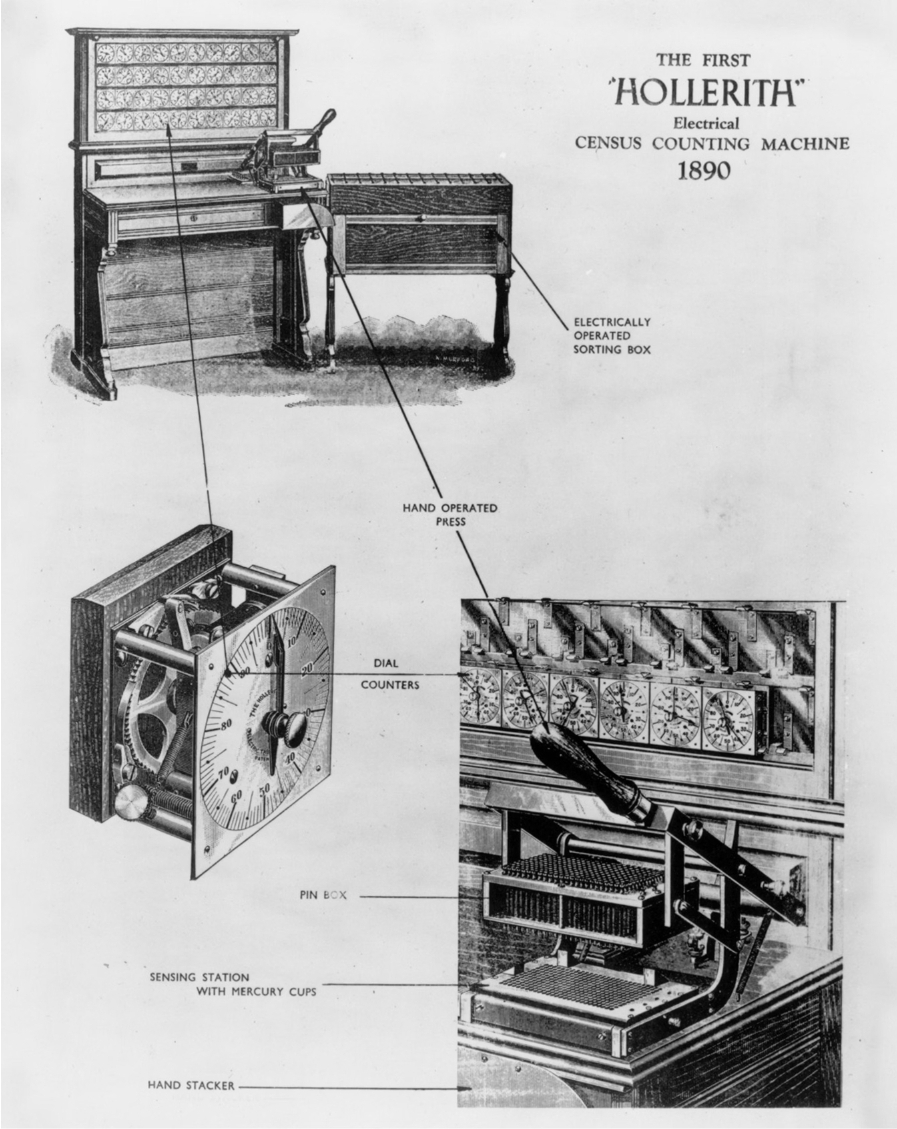
\includegraphics[width=0.6\textwidth]{figuras/cap.3/hollerith_1890_product_sheet.png}
  \caption[Folha de produto da máquina de tabulação de Hollerith (1890)]{Folha de produto de 1890 anunciando \enquote{The First Hollerith Electrical Census Counting Machine}, a máquina eletromecânica de tabulação por cartões perfurados empregada no censo estadunidense de 1890.} 
  \label{fig:maquina_hollerith}
  \fonte{\textcite{IBM_HollerithTabulator}. Disponível em: \url{https://www.ibm.com/history/punched-card-tabulator}. Acesso em: \today.}
\end{figure}

Antes de seguir essa linha, detenho-me num fio que vem do capítulo~\ref{capitulo2} e que prefiro não soltar ainda. Lá rastreei, na obra de Latour, a tensão entre a figuração militar do alistamento e a figuração têxtil da trama, e sustentei, com Haraway, que importa com que figurações se pensa, porque cada uma faz aparecer um mundo e deixa outros na sombra \parencite{Haraway2023Ficar}. Levo esse cuidado comigo ao voltar-me para a história da computação que desemboca na \texttt{IBM}, porque a história que se conta com mais frequência, a que vai da máquina de Hollerith ao computador eletrônico e daí à inteligência artificial, é uma história em que computar foi, desde sempre, calcular com números e com máquinas em uma escala ascendente contínua de desenvolvimento tecnológico. Outras histórias, porém, foram tecidas com outras matérias, e uma delas me interessa de perto, porque computa com fios e nós, e porque, ao computar, também conta histórias. O \textit{khipu} andino, do quéchua \textit{khipu}, \enquote{nó}, era um aparato de cordéis atados, um cordel principal do qual pendiam cordéis secundários (Figura~\ref{fig:khipu_chancay_huando}), em que os povos dos Andes, e de modo notável o Estado inca entre cerca de 1450 e 1532, inscreviam em um só gesto o que se conta e sobre o que se conta, de um lado, censos, tributos e calendários; de outro, genealogias, feitos e histórias de pessoas, de lugares e de tempos \parencite{urton2003signs, quilter2002narrative}.\footnote{Traduzo por \enquote{cordel} o termo \textit{cord} de Urton, que nomeia tanto o cordel principal quanto os pendentes. A palavra carrega, em português, a ressonância com a literatura de cordel, e a acolho de propósito. Como o folheto pendurado em barbante, o \textit{khipu} conta e reconta, e a coincidência reforça a figuração têxtil com que penso este aparato.} Os primeiros cronistas espanhóis já notaram essa dupla natureza, ao verem os guardiões dos fios ora desatar e reatar nós para acertar as contas de um depósito, ora recitar, a partir das mesmas cordas, a memória de feitos passados \parencite[p.~67]{quilter2002narrative}. O subtítulo do volume que Jeffrey Quilter e Gary Urton organizam, \emph{accounting and recounting}, nomeia essa indistinção, e o português a aproxima mais do que o inglês, porque \enquote{contar} é ao mesmo tempo enumerar e narrar, e \enquote{conta} e \enquote{conto} partilham a raiz.\footnote{Urton mostra que a própria separação entre \textit{khipu} numérico e \textit{khipu} narrativo começa a se desfazer quando se olha de perto, porque os mesmos traços, a cor, o sentido da torção, a oposição entre o claro e o escuro, carregam ao mesmo tempo a soma e o sentido que a ordena \parencite{quilter2002narrative}.}

A estrutura dos \textit{khipus} também se fazia por um sistema binário, a direção da fiação e da torção do fio, o sentido em que o nó era atado, a cor, o número, cada traço abrindo uma escolha entre dois estados, e o conjunto deles compondo o que Urton descreve como sequências de sete dígitos binários, sete \textit{bits}, à maneira como a computação eletrônica compõe cada caractere numa sequência de \textit{bits} \parencite[pp.~1--2, 109--117]{urton2003signs}. O computador chegou à codificação binária por tentativa e erro, ao passo que o \textit{khipu} já era, por sua própria natureza, um dispositivo binário, porque a sua matéria, o fio que se fia em um sentido ou em um outro, o nó que se ata por um lado ou por outro, é feita de pares de alternativas \parencite[p.~109]{urton2003signs}. Tanto o sete do \textit{khipu} quanto o oito da computação são escolhas, e nada na lógica do dois estados obriga ao oito; ela exige apenas que cada dígito decida entre 0 e 1, e nada diz quantos dígitos reunir em uma unidade, tanto que máquinas distintas já agruparam os \textit{bits} de seis em seis, de sete em sete, de doze em doze \parencite[pp.~115--117]{urton2003signs}.\footnote{O padrão de codificação de caracteres que se tornou corrente, o \texttt{ASCII}, fixou-se em sete \textit{bits}; foi a \texttt{IBM} que estabeleceu o agrupamento de oito, o \textit{byte}, como unidade ao projetar o \texttt{System/360} em 1964, e foi pela compatibilidade que esse sistema impôs ao mercado que o oito se generalizou a ponto de hoje parecer natural \parencite{Pugh1995Building, Cortada2019IBM}. O ponto que retenho é quem fixou o número: o oito não é propriedade da máquina nem exigência da lógica, e sim sedimento de uma decisão da \texttt{IBM} que perdurou. É mais uma vez a mesma empresa a determinar o rumo de uma tecnologia, impondo como padrão universal uma escolha que poderia ter sido outra, e é esse poder de fixar o que conta como padrão que sigo ao longo deste capítulo, quando descrevo a \texttt{IBM} a fazer-se ponto de passagem.} Falta-nos ainda a tradução que permitiria ler a maior parte do que os \textit{khipu} inscreveram, de modo que o sistema é conhecido na sua estrutura sem que se leia o seu conteúdo.

Quem fiava, atava e lia esses fios, o \textit{khipukamayuq}, o \enquote{guardião dos nós}, ocupava posição em uma hierarquia administrativa, de modo que computar com fios já supunha, ali, uma divisão do trabalho entre quem detinha a regra e quem a executava, à maneira do altar védico que Pasquinelli descreve como exemplo primordial de cultura algorítmica.\footnote{Pasquinelli toma a construção do altar de fogo védico, o \textit{agnicayana}, dispondo milhares de tijolos na forma de um falcão segundo medidas prescritas, como caso primordial do que chama de cultura algorítmica. O resultado dependia de executar com as mãos um procedimento formulado de antemão, e regra e execução já estavam separadas em posições distintas, os sacerdotes que detinham o procedimento e os que erguiam o altar, de modo que a abstração algorítmica nasce, para ele, de uma prática coletiva e material atravessada por uma divisão do trabalho, e não de uma mente que calcula sozinha \parencite[cap.~1]{Pasquinelli_EyeMaster_2023}. É essa divisão que reencontro no \textit{khipukamayuq}, e que voltará, adiante neste capítulo, na separação entre quem concebe e quem executa os sistemas de IA.}

Trago o \textit{khipu}, assim como o altar védico, como uma dessas imagens antigas, de outro canto do mundo, que invoco para pensar com elas, não só como outros modos de computar as coisas e o mundo, mas, sobretudo, no sentido em que importa os modos com que se pensa e que se usa para contar histórias \parencite{Haraway2023Ficar}. O que me interessa nelas é que desfazem a história, tantas vezes contada, inclusive pela própria história da matemática, em que calcular e pensar com sofisticação seriam invenções do Ocidente moderno. Carlo Severi mostra, ao analisar o \textit{khipu}, que a oposição herdada entre \enquote{escrita verdadeira} e \enquote{mero dispositivo de memória} é frágil e etnocêntrica, e que o \textit{khipu} não é um híbrido indisciplinado a desafiar as nossas categorias, mas um artefato mental que se compreende nos seus próprios termos, no qual atua um pensamento matemático complexo que confere ao cálculo um poder aplicável a uma gama crescente de objetos \parencite[pp.~66--70, 90--93]{Severi2018Imagination}. Computar, ali, era uma arte da memória de alta elaboração lógica.\footnote{Detenho-me ainda num fio que me chama a atenção e que registro como tal, sem resolvê-lo. Urton observa que não chegou até nós relato colonial sobre quem materialmente fazia os \textit{khipu}, e trabalha por inferência: as habilidades de produzi-los, fiar, torcer, tingir e dar nós, eram as da tecelagem cotidiana, ofício largamente feminino nos Andes, e a única imagem de que ele dispõe de pessoas a fiar essa matéria é o desenho de Guaman Poma das \textit{acllaconas}, as \enquote{mulheres escolhidas} (Figura~\ref{fig:acllaconas_fiando}) \parencite[pp.~120--124, fig.~5.3]{urton2003signs}. A rima que me detém é minha, não de Urton: a matéria e as técnicas do \textit{khipu} eram as da tecelagem feminina, ao passo que o \textit{khipukamayuq} que as crônicas nomeiam como guardião dos fios comparece sempre como figura masculina e oficial, e essa cena, a das mãos de mulheres num trabalho que depois some do relato, reaparece no início deste capítulo, nas calculadoras humanas, em sua maioria mulheres, que somavam o mundo antes da máquina de Hollerith.}

\begin{figure}[htbp]
  \centering
  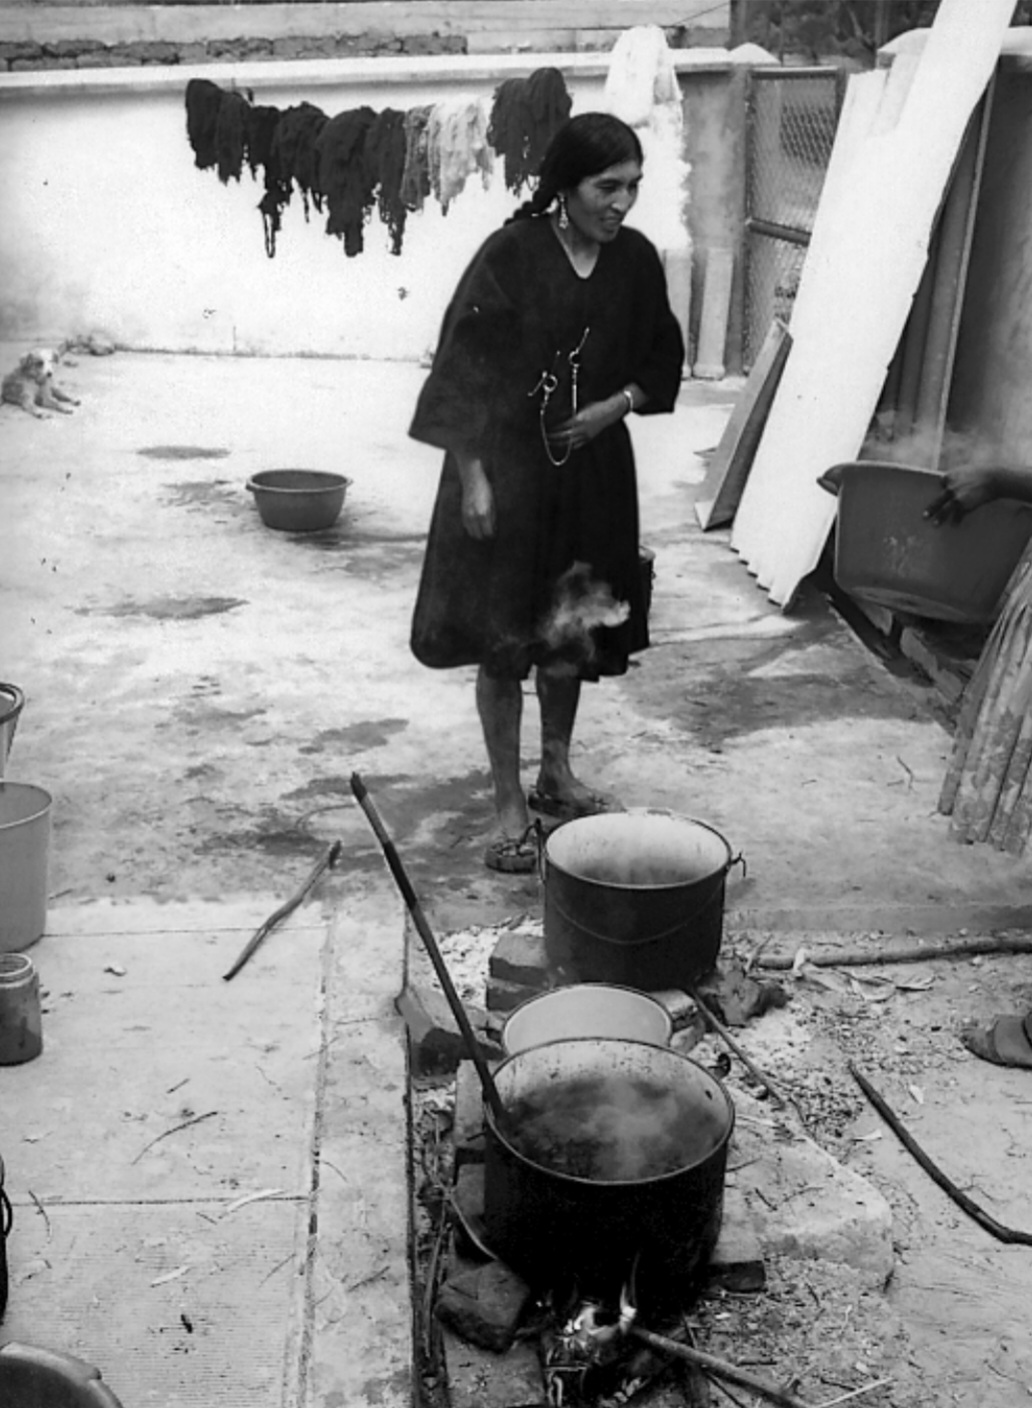
\includegraphics[width=0.6\textwidth]{figuras/cap.3/guaman_poma_acllaconas_fiando.png}
  \caption[\textit{Acllaconas} fiando, em Guaman Poma (1615)]{As \textit{acllaconas}, \enquote{mulheres escolhidas} ou \enquote{virgens do Sol}, em pleno trabalho de fiação. O desenho é a única imagem de que Urton dispõe de pessoas a fiar a matéria de que se faziam os \textit{khipu}, e as figuras retratadas são mulheres.\protect\footnote{A imagem não é registro direto da prática inca, e sim um desenho situado. Guaman Poma de Ayala, autor andino letrado, desenhou-a a pena e tinta por volta de 1615, entre as quase quatrocentas ilustrações de página inteira da \textit{Nueva corónica y buen gobierno}, manuscrito que escreveu e ilustrou pela própria mão como carta ao rei da Espanha. Como não havia, nos Andes, tradição pré-hispânica de imagens em tinta sobre papel, o desenho cruza convenções pictóricas europeias, a moldura, a composição, o texto alfabético junto à imagem, com a abstração geométrica dos têxteis e da cerâmica andinos \parencite{Adorno2000Writing}. A cena chega a Urton, e a mim, já traduzida por essa mão e por esse propósito, o que não a desqualifica como fonte, mas a inscreve, ela também, numa posição.}}
  \label{fig:acllaconas_fiando}
  \fonte{Guaman Poma de Ayala (1615, fol.~298 [273]), reproduzido em \textcite[fig.~5.3]{urton2003signs}. Fac-símile digital disponível em: \url{https://poma.kb.dk/permalink/2006/poma/298/es/image/}. Acesso em: 14 jun. 2026.}
\end{figure}

Há, porém, uma diferença que me interessa guardar, e que não desfaz a aproximação, antes a torce. Os números da computação eletrônica, e os da inteligência artificial, também contam histórias, mas o fazem ao contrário do \textit{khipu}. Onde o cordel inscreve a conta e o conto em um só gesto, à flor da matéria, o número eletrônico se faz signo cuja serventia é justamente comprimir a história, abstraí-la do fio, do corpo e do lugar de onde partiu, e fazê-la circular leve e combinável. O \textit{khipu} mostra a sua trama; o número a esconde. A história não desaparece, mas tem de ser desencavada, porque cada passo da cadeia ganha em forma, em combinabilidade e em mobilidade o que perde em localidade, em particularidade e em matéria \parencite{Latour2017Esperanca}. É esse soterramento, e não a ausência de narrativa, o que separa o cordel andino da grade de coeficientes a que chego no \texttt{Spira}. Pensar com essa outra figuração, a do cordel que conta e reconta, números e estórias, faz o trabalho, no sentido de Haraway, de não naturalizar a figuração herdada. A tabulação mecânica de Hollerith, à qual chego em seguida, é uma forma de contar entre outras possíveis, e o capítulo~\ref{capitulo4} reencontrará essa indistinção entre calcular e narrar no \texttt{Spira}, onde a voz de um paciente é ao mesmo tempo calculada em coeficientes e narrada como sintoma, como vírus e como enfermaria.

\begin{figure}[!htb]
  \centering
  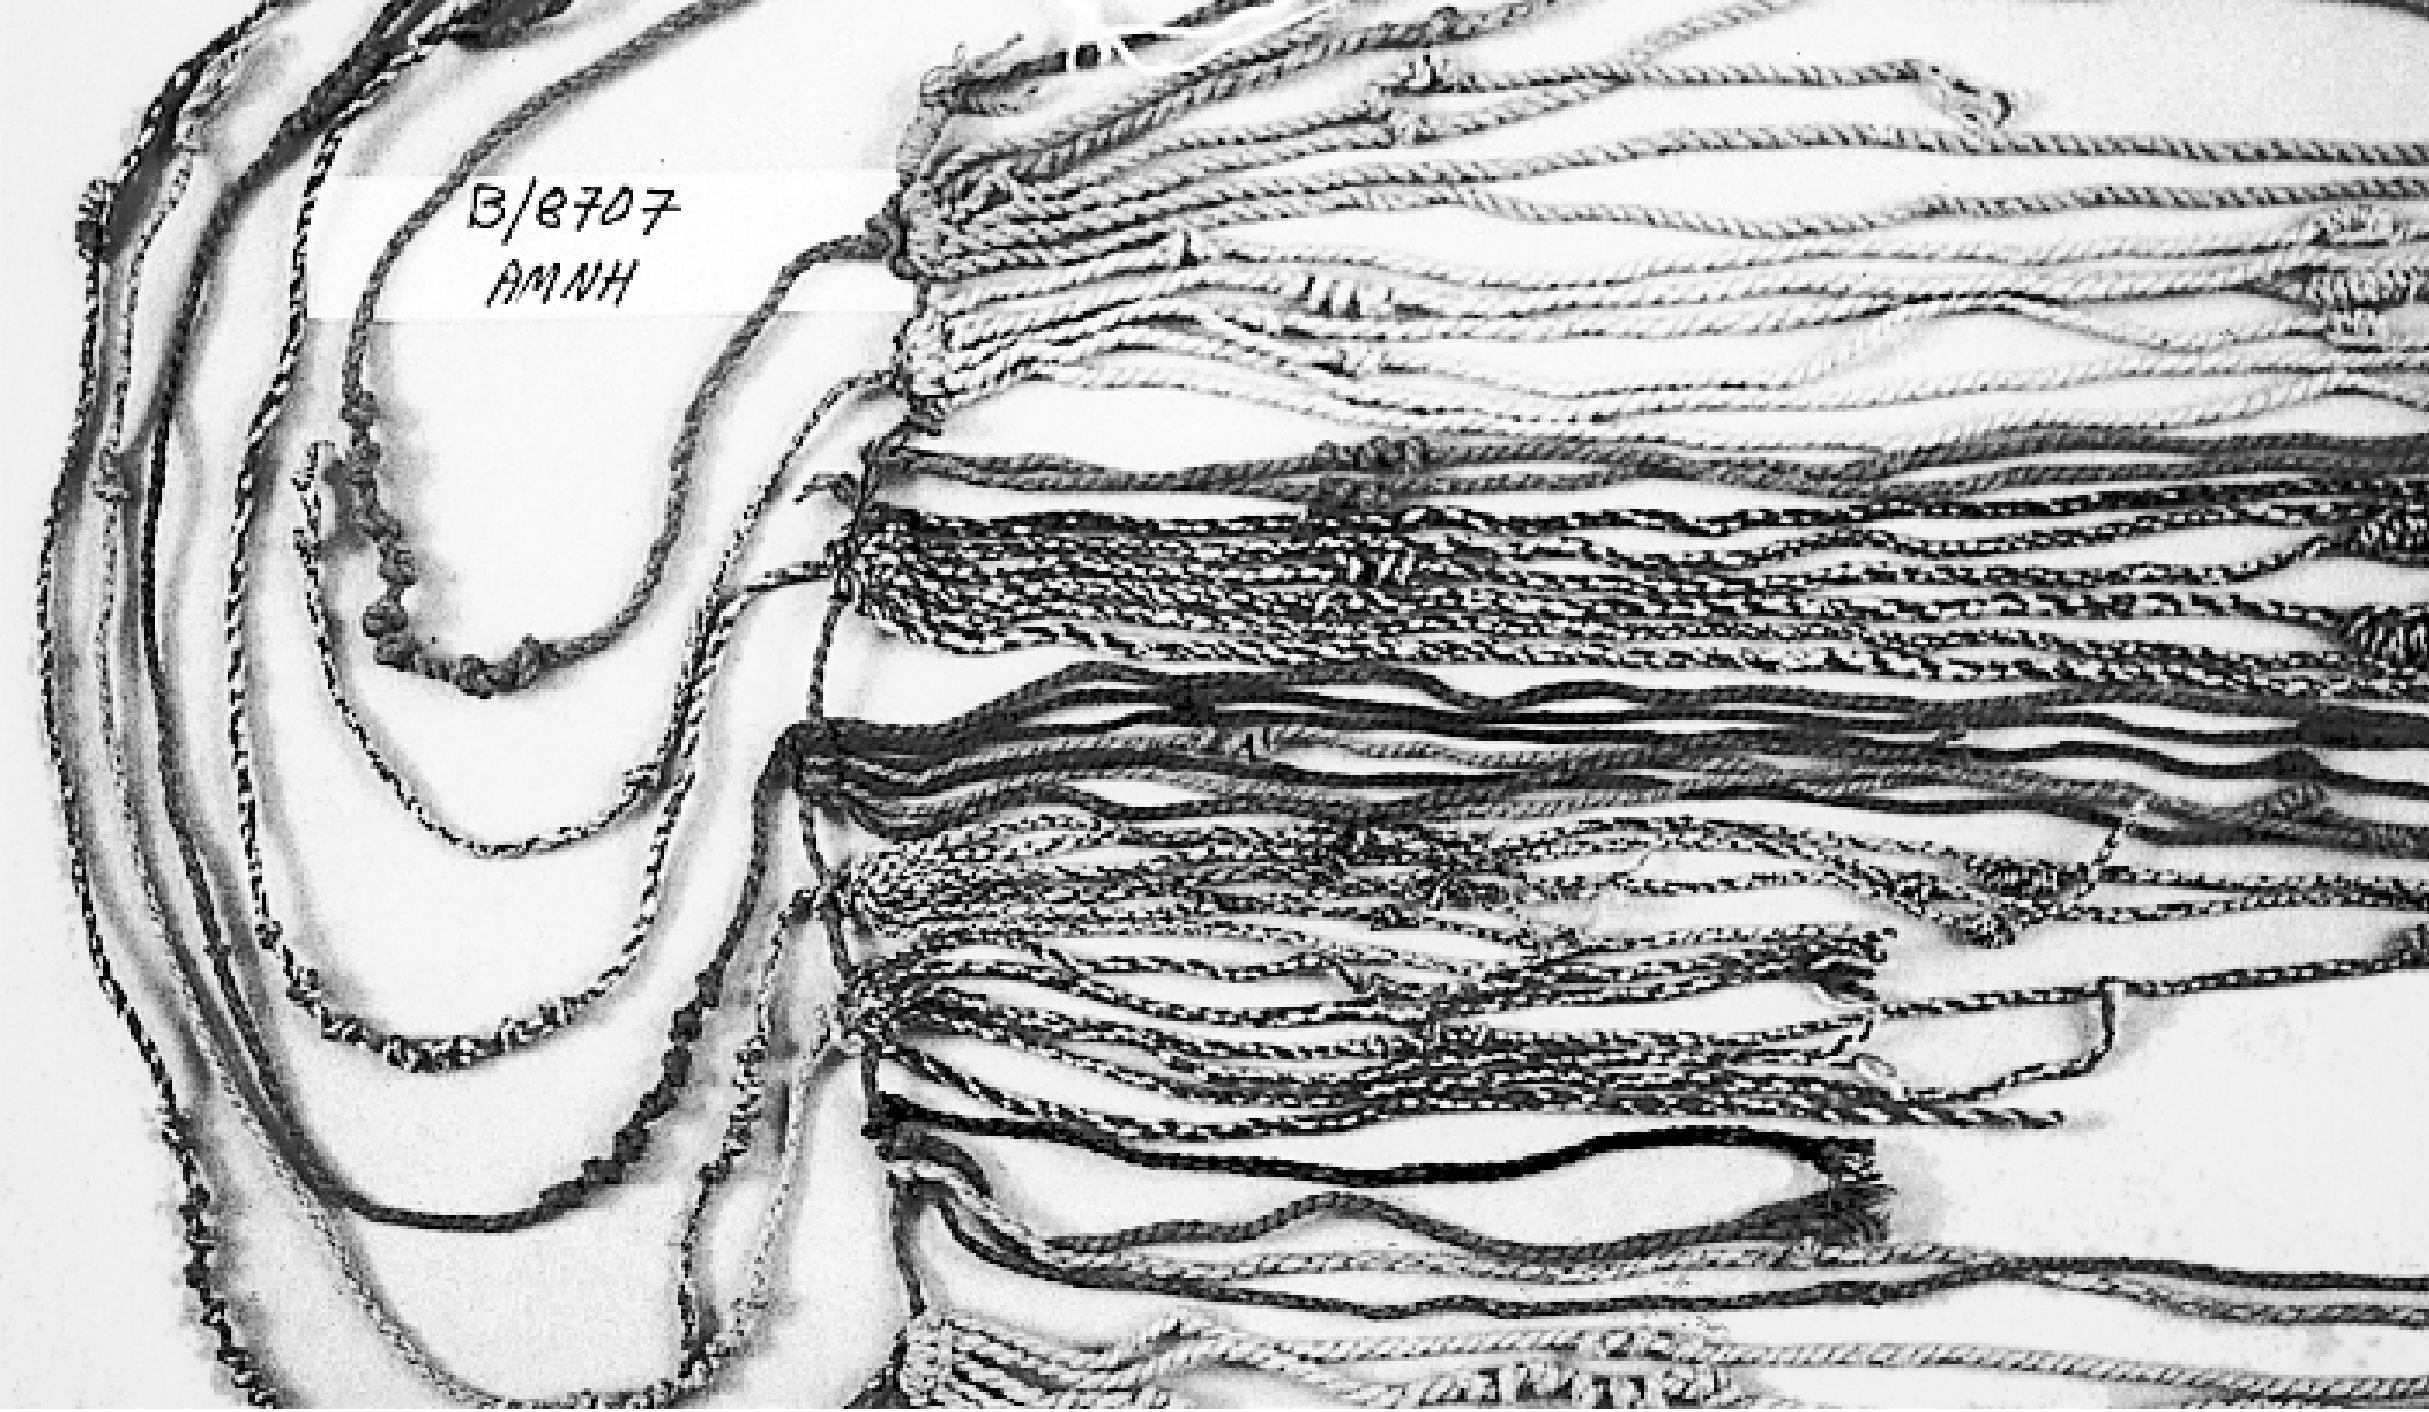
\includegraphics[width=0.6\textwidth]{figuras/cap.3/khipu_chancay_huando_amnh_b8707.png}
  \caption[\textit{khipu} da região de Chancay-Huando (AMNH B/8707)]{\textbf{\textit{khipu} da região de Chancay-Huando, costa central do Peru (AMNH B/8707).} O cordel principal, à esquerda, recolhe os cordéis pendentes em que a informação se inscreve pela cor, pela direção da fiação e da torção do fio, pelo sentido em que cada nó é atado e pela posição que ocupa. Urton lê esse aparato como exemplo de codificação binária, com cada traço abrindo uma escolha entre dois estados. Reproduzido de \textcite[p.~64]{urton2003signs}; acervo do \texttt{American Museum of Natural History}.}
  \label{fig:khipu_chancay_huando}
\end{figure}

Há uma escala nova em questão quando chego a Hollerith. O mesmo movimento de industrialização e urbanização que, nas sociedades modernas, fez crescer e adensar as populações fez também crescer a tarefa de contá-las, até que a contagem manual não desse mais conta: o censo estadunidense de 1880 levara cerca de oito anos para ser tabulado à mão, e o de 1890, diante de uma população ainda maior, ameaçava não ficar pronto antes do censo seguinte, e foi a esse impasse de escala que a tabulação por cartão perfurado de Hollerith respondeu \parencite{Austrian1982Hollerith}. Há aqui, portanto, uma relação de correspondência, em que contar uma população em escala industrial é parte do mesmo processo que produziu as populações a contar e os meios de o fazer. Com essas máquinas, observam Wiggins e Jones, tornou-se concebível registrar uma nação inteira num único arquivo manipulável de forma mecânica, e os grandes esforços de coleta fizeram do Estado, da população e da economia objetos de um novo tipo de conhecimento e de ação \parencite{Wiggins2023Data}.

Mas a máquina tabuladora automatiza em escala industrial o que outras sociedades, como a andina com os \textit{khipus}, já faziam de outra maneira: computar é uma prática antiga, plural e situada. A tabuladora e o \textit{khipu} são dois entre tantos objetos técnicos de contagem que precederam o computador eletrônico e o cercam, ao lado dos ossos entalhados com marcas do paleolítico africano, das fichas de argila (\emph{tokens}) com que a Mesopotâmia registrava bens antes mesmo da escrita, do ábaco em suas muitas formas, da Roma antiga ao \textit{suanpan} chinês e ao \textit{soroban} japonês, e da régua de cálculo dos engenheiros até há poucas décadas, cada um contando à sua maneira e com a sua matéria, sem que um seja ensaio de progresso do seguinte. Se ao cordel se atribui, entre outros usos, o registro de censos e tributos para um Estado, e à máquina de Hollerith o mesmo para outro, é porque contar uma população é sempre um modo de a tornar cognoscível por quem conta, à flor da matéria no \textit{khipu}, soterrado no cartão perfurado. D'Ignazio e Klein argumentam que decidir o que entra na contagem, e como se classifica o que foi contado, é ele próprio exercício de poder, e que esses sistemas se naturalizam como \enquote{o jeito que as coisas são} até que uma controvérsia os reabra; elas nomeiam ainda o paradoxo da exposição, a dupla amarra em que quem mais teria a ganhar ao ser contado é também quem mais se arrisca ao sê-lo \parencite{DIganzio2020Data}.

Essa relação entre contar, classificar e governar encontra ressonância desde Michel Foucault com o conceito de \textit{governamentalidade}, e é pensando com esse conceito, também, que sigo a trajetória da \texttt{IBM}.\footnote{Tomo a governamentalidade no sentido que Foucault assenta no curso \textit{Segurança, Território, População}: a arte de governar que toma a população por objeto e a economia política do saber, e que, em vez de proibir pela lei ou disciplinar corpo, conduz as condutas pela regulação de regularidades no nível do agregado, trabalhando com o provável e o aleatório, com taxas, médias e curvas de distribuição \parencite{Foucault2008Seguranca}. A biopolítica, que Foucault desenvolve nos cursos seguintes, é uma das tecnologias desse governo da população, a que incide sobre os processos biológicos da espécie, o nascer, o adoecer, o respirar e o morrer, tomados como objeto de cálculo e de gestão \parencite{Foucault2008Biopolitica, Foucault1999Defender}. Cito a distinção sem alongá-la, dado o quanto esses conceitos já foram discutidos nas ciências sociais, e guardo dela a ideia de que conhecer a população e governá-la são parte do mesmo processo, e que isto incide tanto sobre o agregado demográfico quanto sobre as vidas humanas e não humanas que o compõe.} A estatística, argumenta Foucault, é uma condição técnica da governamentalidade: a população só passa a ser governada dessa maneira depois que certos aspectos da vida, como a natalidade, a morbidade e a mortalidade, se fazem indicadores e, assim, categorias que podem ser computadas. O que guardo do conceito é que se trata de uma forma de poder que governa uma população desde o próprio ato de torná-la conhecida estatisticamente, e é isso que permeia a estatística setecentista, as máquinas tabuladoras de Hollerith e, a partir delas, a IA preditiva, que herda e radicaliza o cálculo de regularidades sobre populações. Vale notar que o estatístico Leo Breiman, ao mapear o seu próprio campo, separou essas formas de calcular não como dois métodos, mas como duas \enquote{culturas}, isto é, dois modos de crença sobre o que os dados são e sobre o que conta como conhecimento válido.\footnote{Em \enquote{Statistical Modeling: The Two Cultures}, Breiman opôs duas culturas no uso da modelagem estatística: uma que supõe os dados gerados por um modelo estocástico dado e busca explicá-los, e outra que trata o mecanismo gerador como desconhecido e usa modelos algorítmicos apenas para predizer \parencite{Breiman2001Cultures}. À primeira ele atribuía a quase totalidade dos estatísticos, e descrevia a adesão a ela em termos quase religiosos, em que o modelo, uma vez feito, se torna verdade; a segunda, minoritária à época e povoada por jovens da computação, é a que veio a prevalecer e da qual descende o que hoje se chama \emph{predictive modeling} (modelagem preditiva), \emph{predictive analytics} (análise preditiva) em uso comercial, assentada no \emph{machine learning} (aprendizado de máquina), em especial no aprendizado supervisionado, que aprende padrões a partir de exemplos rotulados para estimar desfechos em casos novos. O que ela busca é acertar o que ocorrerá, e contenta-se com correlações que funcionem, sem relação de causa estabelecida. Que um estatístico tenha nomeado a divisão como de culturas, e não de técnicas, é importante, pois a passagem ao cálculo preditivo é uma disputa situada dentro da própria tecnociência que são bases para a IA. Há ainda um grau seguinte, a \emph{prescriptive analytics} (análise prescritiva), em que a diferença para a preditiva é a de quem decide. A análise preditiva estima o que vai acontecer e entrega esse cálculo a uma pessoa, que decide o que fazer com ele; a prescritiva acrescenta à predição um aparato de regras e de otimização que já recomenda, e por vezes executa, a ação a tomar, de modo que a decisão antes reservada a quem recebia o cálculo passa a ser delegada ao próprio sistema. É nessa delegação que reconheço a passagem da predição ao controle de que trato adiante, é a computação, e não mais quem a recebe, que passa a decidir.} 

Essa leitura não é só de Breiman. Nos estudos de ciência e tecnologia, Johnson e Lenhard descrevem culturas de predição em que a matematização, a epistemologia, a tecnologia e a organização social do trabalho científico coevoluem, de modo que cada modo de predizer carrega consigo uma forma de fazer ciência e de organizá-la \parencite{JohnsonLenhard2024}. As duas fontes, de campos distintos, convergem em que predizer é uma prática situada, atravessada por crenças, técnicas e poder. Aprendi isso também de dentro, ao fazer os cursos de estatística e de aprendizado de máquina que descrevo no capítulo~\ref{capitulo1}. Logo na primeira aula, o professor abriu o curso afirmando que a probabilidade é um tipo de pensamento que se aprende, e não uma teoria, e que importa ter dela um conhecimento intuitivo, pois há \enquote{toda uma intuição por trás} dos métodos (figura~\ref{fig:caderno-rodrigues-aula1}).\footnote{Anotações do meu caderno de campo da primeira aula do curso \textit{Fundamentos de Probabilidade e Estatística para Ciência de Dados} (ICMC-USP, Prof.~Dr. Francisco~A. Rodrigues), em 28 de julho de 2025 \parencite{Rodrigues2024ProbEstat}. As frases entre aspas reproduzem o que registrei da fala do professor durante a aula.} Naquela aula, ele distinguiu a inferência da predição por dois verbos, inferir é encontrar, predizer é adivinhar, e apresentou a estatística bayesiana como uma \enquote{atualização da crença}, em que uma probabilidade inicial, o \emph{priori}, se revê diante de novos dados. Em uma aula seguinte, ao introduzir a simulação computacional, definiu o computador como o laboratório onde se aprendem esses conceitos. Tomadas em conjunto, essas formulações de campo exemplificam a virada de que trato aqui: o cálculo probabilístico é ensinado como um modo de pensar, atravessado por intuição e por crença, e não como teoria neutra; a sua finalidade desloca-se do encontrar ao adivinhar, da inferência que busca a estrutura à predição que estima o que vem; e o seu lugar de exercício passa a ser o computador, que simula, calcula e prediz. É nesse deslocamento, da estatística para a computação, que a cultura preditiva se assenta. Essa história, a que liga a estatística e classifica ao cálculo preditivo computacional, já foi investigada por Wiggins e Jones ao argumentarem que os dados são produzidos, e que censos e levantamentos constituem a população como objeto de ação governamental, chegando por essa via a Foucault e à historiografia da quantificação dos povos \parencite{Wiggins2023Data}. Retomo essa história de um jeito diferente, por meio da etnografia do \texttt{C4AI} e de documentos, em que os relatórios anuais, o Acordo de Cooperação e as comunicações institucionais do \texttt{C4AI} e da \texttt{IBM} me deixam seguir. A trajetória de mais de um século que sigo neste capítulo é essa história lida de uma posição situada, a de quem acompanhou um arranjo entre universidade pública e corporação e o viu encerrar-se.

A principal diferença ocorre, sobretudo, na escala e na direção que a IA atual toma. Onde o censo contava o que acontecia ou o que já havia acontecido, os sistemas de IA de hoje calculam o que ainda não aconteceu e fornecem material para se pensar e agir sobre o conteúdo da predição; por exemplo, ao estimar a probabilidade, isto é a chance de um determinado evento ocorrer, de uma região concentrar crimes e para lá dirigir o policiamento, ao atribuir a cada pessoa um escore de crédito que decide quem obtém empréstimo, ou ao ordenar, em uma fila de atendimento em saúde ou de benefício social, quem é triado primeiro. Lidar com a incerteza do futuro para decidir sobre o presente é mais antigo que a IA. A própria probabilidade, condição da governamentalidade de que trato, já era uma forma de fazê-lo, calcular regularidades, estimar o provável, calcular os riscos, saber quais são as chances. O que a IA preditiva acrescenta é uma pretensão nova, a de controlar o futuro, e não só de calculá-lo, mas também para agir desde já sobre o que ainda não aconteceu para que aconteça, ou deixe de acontecer, conforme o planejado. O policiamento que se dirige a uma região antes do crime, o crédito que se nega antes da inadimplência, a triagem que se decide antes do agravo; em cada caso, a predição intervém no porvir mais do que o descreve. Vale, de passagem, um paralelo que tomo com parcimônia, com o oráculo de veneno que Evans-Pritchard descreveu entre os Azande que era também um modo de decidir diante do incerto, e era sobre o seu veredito que se julgavam disputas e se lançavam sentenças \parencite{EvansPritchard2005Bruxaria}. A confiança no oráculo vinha da imprevisibilidade da reação da ave, daquilo que escapava ao cálculo humano; a confiança na IA vem do oposto, de ela pôr a incerteza em números, ao dizer que algo tem tantos por cento de chance de acontecer ou não acontecer, e é esse grau de certeza calculado a partir de exemplos passados que a faz ter tida confiável e governável.

\begin{figure}[H]
  \centering
  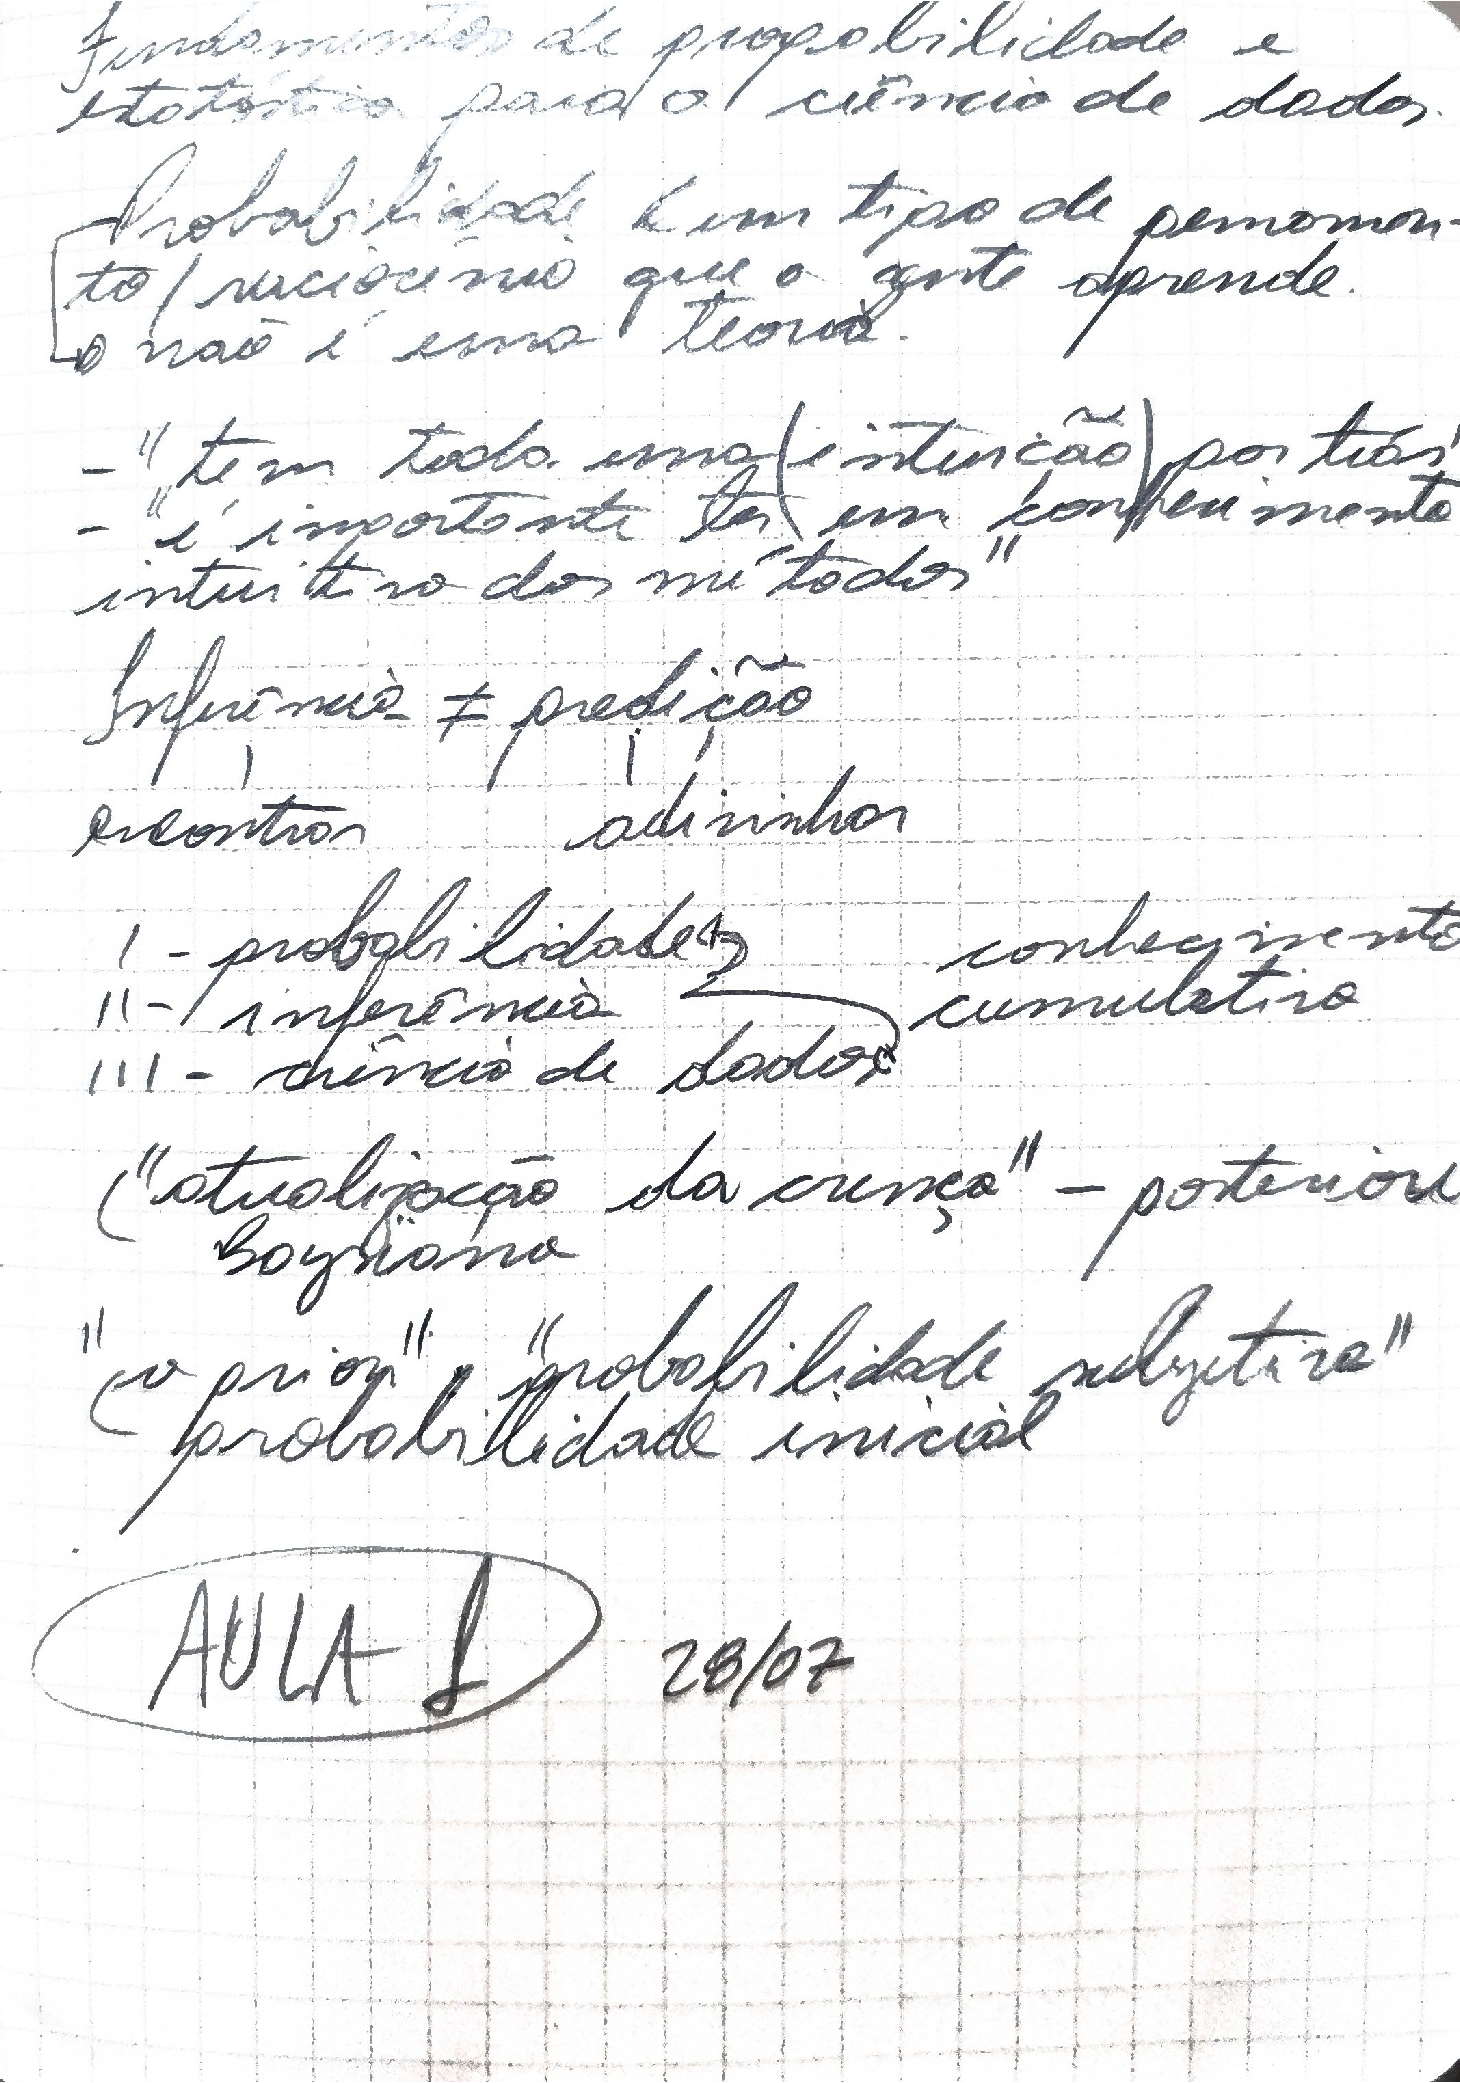
\includegraphics[width=0.85\textwidth]{figuras/cap.3/caderno_rodrigues_aula1.pdf}
  \caption[Caderno de campo: primeira aula do curso de probabilidade e estatística (28/07/2025)]{Página do meu caderno de campo referente à primeira aula do curso \textit{Fundamentos de Probabilidade e Estatística para Ciência de Dados} (ICMC-USP, Prof.~Dr. Francisco~A. Rodrigues), em 28 de julho de 2025. As anotações registram que a probabilidade é \enquote{um tipo de pensamento/raciocínio que a gente aprende} e que \enquote{não é uma teoria}, que \enquote{tem toda uma intuição por trás} e que \enquote{é importante ter um conhecimento intuitivo dos métodos}; a distinção \enquote{inferência $\neq$ predição}, glosada pelos verbos \enquote{encontrar} e \enquote{adivinhar}; o encadeamento \enquote{probabilidade $+$ inferência $+$ ciência de dados} como \enquote{conhecimento cumulativo}; e a estatística bayesiana como \enquote{atualização da crença}.}
\label{fig:caderno-rodrigues-aula1}
\end{figure}

Desta maneira, a estatística do censo descrevia a população que contava; a IA preditiva vai além e antecipa o que dela se deixa prever, os comportamentos, os riscos, tudo o que se possa estimar como provável a partir do que já foi coletado de exemplos ocorridos no passado. A pandemia de Covid-19 mostrou como isso vem ocorrendo. Os doentes viravam curvas de infectados, taxas de transmissão, projeções de óbitos e de ocupação de leitos, e era sobre esses números que se passou a decidir as medidas de saúde pública. Cada pessoa adoecida entrava no cálculo como ponto de uma curva, do mesmo modo como, no cartão de Hollerith, cada pessoa entrara como categoria perfurada; em ambos, a vida singular se faz dado agregado, e é nessa forma que se torna governável. Esse modo de tornar a vida computável segue em funcionamento e se intensificou como nunca antes. Digitalizar a saúde converte o prontuário em arquivo legível por máquina, datificá-la vai além, e faz do sintoma físico do corpo, do exame e do diagnóstico do paciente pontos de dado sobre os quais se calcula e se decide, como faço no caso do \texttt{Spira}.\footnote{Configurações como essa vêm sendo nomeadas como datificação da vida. O termo \emph{datafication} foi cunhado por \textcite{MayerSchonberger2013Big} para o gesto de pôr um fenômeno em forma quantificada de modo que possa ser tabulado e analisado, e foi deslocado, na crítica que se lhe seguiu, para nomear a conversão da própria vida social em dado e a extração de valor que essa conversão alimenta \parencite{vanDijck2014Datafication, CouldryMejias2019Costs}. O Programa SUS Digital, instituído no Brasil em 2024 e com adesão de todos os 5.570 municípios, dos 26 estados e do Distrito Federal, é um exemplo dessa intensificação. Descreve-se como um conjunto de iniciativas que modernizam o Sistema Único de Saúde por soluções digitais e tem entre suas metas o prontuário eletrônico, o acesso do cidadão aos próprios dados no aplicativo Meu SUS Digital e painéis de monitoramento e relatórios de desempenho que o gestor mobiliza para a tomada de decisão. Disponível em: \url{https://www.gov.br/saude/pt-br/composicao/seidigi/sus-digital}. Acesso em: 16 jun. 2026. Datificar a saúde pode ter efeitos sobre a vida das pessoas, ao antecipar um agravo, ao distribuir melhor um leito, ao devolver ao paciente o acesso ao próprio histórico, etc. O que decide a qualidade desses efeitos é o arranjo que o sustenta, de quem é a infraestrutura que guarda os dados, quem os gere, com quem são compartilhados e a serviço de que fim, questões que retomo no capítulo~\ref{capitulo4} ao seguir o \texttt{Spira} até as condições materiais e institucionais de que depende.} Computar uma população e geri-la passam a ser a mesma coisa, e foi na tecnociência da tabulação que isso deu seus primeiros sinais em escala industrial, quando o censo de 1890 converteu a vida das pessoas em categorias perfuradas no cartão (sexo, raça, idade, nacionalidade, estado civil, profissão, residência). Considero, porém, outras populações. As redes da IA, e as que aqui descrevo, abrangem também não humanos, animais, plantas, territórios, e alcançam, no limite, aquilo que sequer se tem por vivo, os recursos minerais, o clima, um vírus como também sigo no capítulo~\ref{capitulo4}. No \texttt{Spira}, esse converter-se da vida em dado toma a forma de uma cadeia de inscrição: o fôlego de uma pessoa torna-se sinal de áudio, espectrograma e, por fim, coeficiente processável por uma rede neural, no movimento que sigo no capítulo~\ref{capitulo4}. E esse mesmo cálculo, que parece imaterial, repousa sobre um fundo material: há, do outro lado, todo um não vivo arrancado da terra para que a conversão se faça. O mineral, o inerte que o poder extrai e converte em valor, é também a base material da IA,\footnote{A fronteira entre o que conta como vida e o que conta como inerte é o que Elizabeth Povinelli chama de partição entre a Vida e a Não Vida, sobre a qual se exerce o \textit{geontopoder}, modo de governança do liberalismo tardio que separa o domínio do orgânico do domínio do geológico, da rocha e do mineral \parencite{Povinelli2023Geontologias}. É desse \textit{geos}, o polo da Não Vida que o poder extrai, que volto a tratar adiante.} e é o que os estudos críticos rastreiam quando seguem as cadeias globais de extração material, laboral e epistêmica que sustentam esses sistemas, do lítio e do cobalto das minas ao trabalho de quem rotula dados, em especial Crawford e Joler \parencite{Crawford_Joler_CalculatingEmpires_2023, Crawford2018Anatomy} e Pasquinelli \parencite{pasquinelli2020nooscope, Pasquinelli_EyeMaster_2023}.

Há um movimento que me detém neste percurso, e que as figuras do \textit{geos} e do Terrestre me ajudam a pensar. O minério que sustenta a inteligência artificial levou eras geológicas para se depositar na crosta, e quanto mais essa tecnologia se anuncia como futuro, como salto adiante rumo a um mundo cada vez mais tecnológico, mais ela desce ao fundo do tempo da Terra. O circuito que promete o porvir é feito de lítio, de cobalto, de silício, de terras raras, e o vetor que parecia apontar para a frente aponta, ao mesmo tempo, para baixo, para o mineral de que a tecnologia nunca se desprende. Latour dá nome a essa torção quando recusa a flecha que ia do Local atrasado ao Global futuro e a substitui pelo movimento do Moderno ao Terrestre, um descer à terra, algumas dezenas de quilômetros, a Zona Crítica, entre a atmosfera e a rocha, em que a vida e a técnica de fato se sustentam \parencite{Latour2020Onde}. Leio nisso, mais do que um regresso ao passado que apenas reinscreveria a mesma flecha ao contrário, a descoberta de que o futuro tecnológico nunca esteve à frente, e sim embaixo, na matéria de que sempre dependeu.

Antes de seguir essa torção, demoro-me no que a conta dos minérios e dos dados quase sempre deixa de fora: as inúmeras comunidades de seres vivos, humanas e não humanas, que habitam os territórios de onde se extrai a matéria da inteligência artificial, e cujos mundos a mineração desfaz no mesmo gesto com que arranca o minério. É a mesma torção que o \textit{khipu} fez ver no início deste capítulo, quando desfez a linha reta que iria da máquina antiga à inteligência artificial, assim como, computar não foi a invenção de uma máquina por vir, mas permeia práticas antigas, plurais e situadas, o futuro da inteligência artificial parece correr à dependência cada vez mais profunda do \textit{geos}, do mais antigo e mais inerte dos não humanos. E aqui as duas figuras que evoco entram em tensão: o \textit{geos} de Povinelli é a Não Vida, o inerte que o poder extrai e converte, ao passo que o Terrestre de Latour é um \enquote{geo} que reage, que deixou de ser o plano de fundo da ação humana para participar dela, voltando-se contra quem o explora \parencite{Latour2020Gaia}. A inteligência artificial trata o \textit{geos} como matéria, minério a extrair e dado a processar, mas é esse mesmo \textit{geos} que reage, no esgotamento das jazidas e na reação do sistema terrestre, e se recusa a permanecer inerte. Retomo, assim, o fio que assentei no capítulo~\ref{capitulo1}: se ali a rede já não distinguia o humano do não humano, aqui ela não distingue sequer o vivo do inerte, e o mineral, o mais mudo dos actantes, mostra-se capaz de agir. É esse adensamento do \textit{geos} na tecnologia, e a sua recusa em ser mero recurso, o que sigo ao descer com os atores até à Terra de que empresas como a \texttt{IBM} e centros de pesquisa como o \texttt{C4AI} extraem e constroem suas tecnociências. 

Se até a Terra (rea)age, como sustentei há pouco, é porque a rede que sigo não conhece hierarquia entre os seus actantes, e isso exige precisar o que entendo por rede e por agência, a noção que me autoriza a seguir, em um mesmo plano, Fábio, Cláudio, a \texttt{IBM} e a máquina tabuladora. Compreendo a rede, neste capítulo, como um processo de articulação entre atores --- ou actantes, quando quero enfatizar (e não diferenciar), a agência não humana ---\footnote{Uso \enquote{actante} para realçar a agência não humana, no sentido que desenvolvi no capítulo~\ref{capitulo1}, e, como Latour, alterno actante e ator conforme o tipo de agência que quero pôr em relevo. A própria expressão ator-rede funciona como oxímoro, articulação de termos opostos que produz um sentido novo \parencite{latour1996clarifications}.} humanos e não humanos, cuja dinâmica depende de relações materiais, discursivas, simbólicas e institucionais. Interessa-me, sobretudo, o modo como as agências --- e entendo por agência qualquer entidade que age ou à qual uma ação é atribuída, sem supor motivações humanas --- se distribuem pela rede e como se transformam, ao longo do tempo, em distintos regimes sociotécnicos. A rede é, então, a associação entre actantes heterogêneos, individuais ou coletivos, que se definem em boa parte ao longo das próprias cadeias de associação; aquilo que se move e aquilo que é movido não tem forma nem atributos estáveis, e cada ator ganha contorno a partir das relações que estabelece com os outros \parencite{latour1996clarifications}. É esse o sentido em que sigo com Latour e Callon ao longo deste capítulo, e é também o que me permite tratar a translação como a descrição do que sobrevém aos atores e aos objetos quando se associam.

\section{Seguindo Fábio e Cláudio: observação, entrevistas e documentos}
\label{sec:seguindo_atores}

Quando iniciei a pesquisa, o centro estava em consolidação e buscava pesquisadores, financiadores e infraestrutura, que eu denomino por \textbf{aliados}. Tomo \enquote{aliados} e \enquote{alianças} no sentido latouriano de atores, humanos e não humanos, vivos e não vivos, recrutados para sustentar uma controvérsia e estabilizar fatos e artefatos das tecnociências. É vocabulário que pertence à figuração militar-industrial cuja densidade e cujos efeitos analiso no capítulo~\ref{capitulo2}, e o uso aqui com essa consciência. Latour descreveu a ciência como os próprios cientistas a apresentavam e a praticavam, e o vocabulário militar não é, nele, escolha estilística do analista, mas a forma que essa prática assumia em ação. Fábio e Cláudio faziam essa tecnociência. Buscar pesquisadores, financiadores e infraestrutura, sustentar a controvérsia que mantinha o centro de pé, vencer a disputa por recursos, era recrutar aliados no sentido exato em que Latour descreve o gesto, e descrevê-lo assim é fiel ao que eu via em campo. A figuração têxtil de Haraway, que sustento no capítulo~\ref{capitulo2}, faz outra coisa, porque propõe um outro tipo de tecnociência, e eu a mobilizo como figuração de pensamento e como o lugar de onde escrevo esta tese, e não como descrição do que Fábio e Cláudio faziam. Quando descrevo o trabalho deles, descrevo como Latour, porque era assim que eles trabalhavam; quando me posiciono sobre que tecnociência quero fazer, e como quero descrevê-la, é com Haraway que penso. Manter essa distinção visível é o que me permite usar o vocabulário militar aqui no capítulo~\ref{capitulo3} sem o naturalizar, isto é, como figuração que descreve uma prática situada, e não como a única forma de dar a ver o que o centro fazia.\footnote{Eu também me tornei uma \enquote{aliada} e, além de realizar esta pesquisa sobre eles, passei a fazer parte do grupo de humanidades do \texttt{C4AI}, o Observatório de IA: impactos e regulação (\texttt{OBIA@C4AI}).} Essa presença em toda parte foi ainda amplificada pelo isolamento da pandemia de Covid-19 (2020-2023), que afastou os encontros presenciais e empurrou a vida do centro para os espaços públicos controlados e digitais em que eu os encontrava, esses mesmos espaços que configuraram o que seria um laboratório de inteligência artificial para esta tese, conforme discuto nos capítulos~\ref{capitulo1} e~\ref{capitulo4}.\footnote{Apresentei a origem institucional do \texttt{C4AI}, sua fundação em outubro de 2020 em plena pandemia, o arranjo \texttt{USP}-\texttt{FAPESP}-\texttt{IBM} no âmbito dos Centros de Pesquisa em Engenharia da \texttt{FAPESP} e a configuração do centro como laboratório distribuído, no capítulo~\ref{capitulo1}. Retenho aqui o que importa ao argumento deste capítulo. O \texttt{C4AI} conta ainda com três instituições associadas, \texttt{ITA}, PUC-SP e \texttt{FEI}, e integrava a \texttt{IBM} AI Horizons Network (AIHN), rede global de centros de pesquisa universitários que a \texttt{IBM} estabeleceu em 2016 para \enquote{acelerar pesquisa e aplicação de IA} através de colaborações com \enquote{universidades líderes}. Essa formulação pede análise, ao posicionar a \texttt{IBM} como articuladora central de uma rede global em que as universidades, ainda que descritas como \enquote{líderes}, atuam dentro de um ecossistema estruturado por prioridades e infraestruturas corporativas. Para informações institucionais do \texttt{C4AI}, ver: \url{https://c4ai.inova.usp.br/about.html}. Acesso em: 30 nov. 2025.} Foi assim que Fábio e Cláudio passaram a comparecer falando em nome do centro como porta-vozes,\footnote{Retomo \enquote{porta-voz} no sentido que assentei no capítulo~\ref{capitulo1}, o de quem fala em nome de entidades, humanas ou não, que dependem de alguém que articule suas posições. Fábio e Cláudio compareciam como porta-vozes do \texttt{C4AI} ao apresentá-lo e representá-lo nos espaços que acompanhei.} atraindo para si as atenções, inclusive a minha. Era comum que apresentassem o centro e suas pesquisas, e a \texttt{IBM} surgia com frequência nessas conversas. \enquote{Quando o C4AI começou havia uma certa dificuldade de saber se a gente ia conseguir agregar tanta gente e como é que a gente ia fazer isso}, contou-me Fábio em entrevista. Foi a participação da \texttt{IBM} que trouxe foco: em \enquote{vários encontros no começo}, definiram \enquote{que não ia fazer muitos projetos para não pulverizar o dinheiro}, e o centro tornou-se \enquote{um centro que, em volta de alguns projetos, que exigem conhecimento de várias fontes, de várias áreas, você tem todo um grupo de gente interessada em IA}.

Ao longo do tempo, porém, essa concentração teve seus efeitos. Quando a \texttt{IBM} reorientou seus interesses nas frentes de saúde e de agronegócio, os projetos correspondentes perderam o financiamento direto do centro, e o quanto a agenda de pesquisa se atava às decisões estratégicas corporativas, que o cotidiano mantinha implícito, tornou-se mais evidente. O \texttt{C4AI}, por sua vez, não parou onde a frente corporativa parou. No mesmo período em que a \texttt{IBM} deixava o setor de saúde, os pesquisadores do centro montaram um centro dedicado ao tema, o Centro de Inteligência Artificial em Gestão em Saúde, aprovado pela \texttt{FAPESP} em 2024, e, enquanto a frente do agronegócio se reorientava, desenvolveram o MClimate, novo desafio de pesquisa voltado à previsão climática por modelagem física. Em ambos os casos, uma frente que perdia o aporte corporativo reaparecia sob outro arranjo de financiamento e outro recorte de pesquisa, por iniciativa dos próprios pesquisadores, e desse percurso resultaram publicações científicas, \textit{datasets} abertos e ferramentas disponibilizadas à comunidade. Deslocamentos como esses são descritos neste capítulo, e não a intenção que os teria guiado nem uma ordem em que a corporação se moveria primeiro e o centro reagiria depois: não tenho como dizer, a partir do que pude seguir, se reancorar uma frente em nova fonte de fomento foi gesto de autonomia diante da \texttt{IBM} ou recomposição da mesma atadura sob outra forma, e as negociações em que isso se decidiu correram por canais que não acompanhei. Descrevo, então, uma rede em que cada ator, corporação, universidade, agência de fomento e pesquisadores, faz associações e desloca o curso das associações, e deixo em aberto o que cada deslocamento significou.

Caminhei conforme fosse preciso, acompanhando as associações onde quer que elas me levassem, e elas pareciam levar-me a Fábio e Cláudio, bem como ao que faziam e diziam. Eles, porém, foram dois entre os atores que acompanhei (como demonstro no capítulo~\ref{capitulo4}, ao apresentar a rede construída por Marcelo). Também observei outros atores e eventos, muitos dos quais ficaram fora da versão final desta tese, mas que estão presentes na perspectiva analítica desta pesquisa e no olhar etnográfico que a permeia. As fronteiras que limitam a extensão da rede a traçar (teórica ou metodologicamente) não estão dadas, e ainda assim preciso começar e parar em algum ponto, ao menos para os fins e objetivos práticos da pesquisa. A ausência de determinados atores é tão consequente analiticamente quanto a sua presença, seja essa ausência intencional ou não. Foram os movimentos desses atores que me levaram a escrever este capítulo, seguindo o caminho que eles me indicavam e que eu queria seguir.

Algoritmos e modelos de linguagem apareceram ao longo dessa caminhada, emergiram na entrevista com Marcelo, em narrativas retrospectivas sobre o desenvolvimento do \texttt{Spira}, e nos artigos científicos que analisei (conforme discuto no capítulo~\ref{capitulo4}). O que me escapou foi o fazer IA em ato, o movimento de construção dos conjuntos de dados e dos modelos propriamente ditos diretamente pelas mãos dos cientistas e engenheiros. Encaro essa inacessibilidade como um limite desta etnografia, em lugar de saldá-la com uma explicação que eu não tenho como sustentar. O que pude seguir foram os relatos sobre esse fazer, e não o fazer no instante em que se dava --- e não seria isso uma maneira de também fazer? ---, e as razões desse limite excedem o que o meu material permite isolar; a pandemia, o modelo de laboratório distribuído e as dinâmicas particulares do \texttt{C4AI} compõem-se, no meu caso, com o que pode ser uma reserva mais ampla do campo diante da observação externa, sem que eu disponha de meios para separar o que pertence a cada um. Deixo a questão nesse ponto, como parte do que a posição de onde descrevo alcança e do que lhe escapa. Esse tipo de limitação, com o tempo, passou a constituir um dos argumentos desta pesquisa, pois Latour sustenta que a distinção entre o \enquote{interior} e o \enquote{exterior} de uma ciência é ela mesma efeito do trabalho científico. O que aparece como interior e o que aparece como exterior são dois lados de um mesmo divisor, erguido pela própria prática, e retomo esse argumento na Lição 1 do capítulo~\ref{capitulo1}, sobre acompanhar a pesquisa em IA enquanto ciência em construção. Lida por essa chave, a opacidade do núcleo técnico deixa de ser a parede em que minha observação esbarrou e passa a ser um efeito do corte que fiz, no sentido de \textcite{strathern2011cortando}.

Seguir Fábio e Cláudio significou estar onde eles estavam, e onde eles estavam era a rede pela qual o \texttt{C4AI} parecia funcionar naquele momento, sem paredes que a fechassem em um \enquote{laboratório} delimitado fisicamente, como discuto no capítulo~\ref{capitulo4} ao seguir a rede que Marcelo construiu.\footnote{Mantive diálogos com pesquisadores vinculados ao \texttt{C4AI} ao longo do trabalho de campo. Essas conversas, sem roteiro estruturado e sem o formato de entrevista formal, foram fonte de dinâmicas cotidianas, tensões não verbalizadas em contextos públicos e percepções sobre o arranjo que por vezes diferiam das narrativas institucionais. A pedido dos interlocutores, não as identifico nominalmente. A escolha responde a uma consideração ética, a de proteger pessoas em posição de menor poder institucional, que poderiam sofrer consequências por declarações críticas, e ao reconhecimento de que o caráter aberto dessas trocas dependia, em parte, da garantia de anonimato. Quando informações dessas conversas informam a análise, apresento-as de modo a preservar o anonimato sem comprometer a integridade interpretativa.} Essa posição tinha o seu preço. O \texttt{C4AI}, distribuído por quatro campi, dezenas de grupos, centenas de pessoas, só comparece como uma coisa só quando alguém o enuncia, e Fábio e Cláudio eram esse alguém. Ao dizerem o que o centro era e o que faziam os seus pesquisadores, não relatavam uma voz que o \texttt{C4AI} já tivesse; davam-lhe uma, e a que lhe davam recortava, entre tudo o que o centro era, a face que cabia no que diziam. Era essa face que eu acessava ao segui-los, nos eventos onde os encontrei. O cotidiano de quem desenvolvia os modelos, coletava os dados, escrevia o código e treinava os algoritmos corria em uma outra camada da rede. Seguir os porta-vozes me pôs diante das estratégias de legitimação, das tensões entre agendas corporativas e acadêmicas, das negociações que sustentam os arranjos de inovação, e deixou fora do meu alcance, as práticas laboratoriais distribuídas, as rotinas dos bolsistas, as decisões técnicas do desenvolvimento dos sistemas. A rede que Fábio e Cláudio teciam era uma parte do \texttt{C4AI}, e o centro permanecia maior do que ela. Sigo certos atores e, ao segui-los, deixo de seguir outros; é dessa parcialidade que esta etnografia se faz, e é ela que a tensiona.

O que descrevo, portanto, é o \texttt{C4AI} a partir de seus porta-vozes e das redes que eles construíam, e foi por aí que cheguei a certas relações que organizam os arranjos público-privados em inteligência artificial. Seguindo Latour, fazer ciência é manipular instrumentos, coletar dados e construir modelos no interior de um laboratório, e é também, e talvez sobretudo, alistar aliados, mobilizar recursos, negociar financiamentos, traduzir interesses, estabilizar redes que permitam aos fatos e artefatos circularem e se sustentarem. Em \textit{Ciência em Ação}, Latour acompanha um \enquote{chefe} de laboratório que passa semanas viajando entre ministérios, indústrias farmacêuticas e universidades, enquanto sua colaboradora permanece na bancada. \enquote{Quem está realmente fazendo pesquisa?}, pergunta Latour. \enquote{Onde é que a pesquisa está de fato sendo feita?} A resposta é que ambos fazem ciência: ela \enquote{é capaz de se dedicar inteiramente ao trabalho de laboratório \textit{porque} o chefe está sempre fora, trazendo para dentro recursos e subsídios novos}.\footnote{\textcite[p.~257]{Latour2011CienciaEmAcao}. Latour conclui: \enquote{a tecnociência tem um lado de dentro porque tem um lado de fora. [\ldots] quanto maior, mais sólida, mais pura a ciência é lá dentro, maior a distância que outros cientistas precisam percorrer lá fora} (p.~258). Seguir os porta-vozes do \texttt{C4AI} por seminários, eventos empresariais e negociações institucionais documentou, portanto, as condições que tornam possível esse fazer.} Fábio negociando com a \texttt{FAPESP}, Cláudio explicando à \texttt{IBM} como o centro pode atender às necessidades do setor, pesquisadores disputando acesso a GPUs, bolsistas publicando em conferências internacionais para legitimar o trabalho do centro: tudo isso é fazer IA. A distinção entre o \enquote{científico} e o \enquote{institucional}, entre o \enquote{técnico} e o \enquote{político}, é ela mesma um efeito das redes que deram certo, e só na aparência precede esse efeito. É uma etnografia do fazer IA nessa dimensão que ofereço, a que mostra as condições de possibilidade para que algoritmos existam, modelos sejam treinados, sistemas sejam desenvolvidos e pesquisas se sustentem no tempo.

Nas notas de campo registrei o que era dito e, com igual atenção, \textit{como} era dito, \textit{onde} era dito e \textit{para quem} era dito. Fábio e Cláudio apresentavam o \texttt{C4AI} de um modo nos contextos acadêmicos, com ênfase em metodologia, rigor científico e contribuições teóricas, e de outro nos contextos empresariais, com ênfase em aplicabilidade, parcerias estratégicas e geração de valor, e essa diferença mostra como a tecnociência circula por registros heterogêneos e se constitui nessa circulação, no transitar entre a universidade e o mercado. É o que Latour documenta no \enquote{chefe} de laboratório, que em um mesmo dia apresenta a pandorina ao ministro da Saúde enfatizando aplicações clínicas, aos colegas da Academia enfatizando rigor metodológico, aos jornalistas enfatizando revolução científica.\footnote{Cf. \textcite[p.~252--255]{Latour2011CienciaEmAcao}. O \enquote{diário} fictício que Latour constrói para acompanhar o chefe de laboratório documenta essa capacidade de circular entre registros heterogêneos: ministérios, indústrias, universidades, hospitais, matadouros.} Essa atenção ao modo do dizer só foi possível a partir de um lugar determinado. Eu estava na audiência daqueles eventos porque o vínculo com o OBIA, o grupo de humanidades do \texttt{C4AI}, me punha ali, e foi esse mesmo vínculo que me deu as discussões institucionais e as conversas informais a que de outro modo eu não chegaria. Anotava-as no caderno de campo que mantinha no aplicativo de notas do celular, e ao lado do que se dizia eu registrava a circunstância da minha presença: de onde eu escutava, como tinha chegado àquela sala, o que a minha entrada pelo OBIA me abria e o que, por ela, me ficava vedado. Ao integrar o OBIA, tornei-me parte da rede que investigava, e essa posição é ela mesma um dos cortes que torna presentes certas relações e deixa outras na sombra. Não há ponto de vista exterior de onde uma rede sociotécnica se deixe contemplar com objetividade, porque quem observa é parte das associações que descreve, e foi de dentro dessa condição que escrevi. O que me coube, então, foi anotar a circunstância da minha presença junto com o que ela me deixava ver, em vez de apagá-la para simular uma vista de lugar nenhum.\footnote{Como argumenta Latour, \enquote{seguir cientistas e engenheiros de verdade} exige \enquote{mais sutileza agora que nosso guia vai vestir muitas máscaras misturadas e seguir por caminhos vários simultaneamente} \parencite[p.~241]{Latour2011CienciaEmAcao}. O rigor está em explicitar a própria posição e os seus efeitos sobre o que dali se alcança e o que dali escapa, em vez de fingir uma neutralidade inexistente.}

Foi sobre esses anos de observação que as entrevistas se assentaram. Conversei com Fábio Cozman em 4 de setembro de 2025 e com Cláudio Pinhanez em 2 de outubro de 2025, cerca de sessenta minutos cada, depois de mais de três anos acompanhando o arranjo, o que me permitiu formular perguntas informadas pelas tensões que a observação havia me deixado entrever de forma fragmentária.\footnote{Ambas as entrevistas foram realizadas em português via Google Meet, transcritas integralmente e analisadas em língua original.} O modo direto com que os dois descreveram o arranjo, Cláudio explicitando a lógica de arbitragem geopolítica ao dizer que \enquote{o estudante é barato demais}, Fábio reconhecendo que projetos perderam financiamento quando a \texttt{IBM} vendeu divisões comerciais, devo em parte à confiança construída ao longo de anos, e em parte ao momento das conversas, realizadas quando o arranjo ainda vigorava no papel, mas já sob tensões que anunciavam seu fim. Foi numa conversa informal com pesquisadores de outros grupos do \texttt{C4AI}, aliás, que soube de algo ainda não público: quando entrevistei Fábio e Cláudio, a \texttt{IBM} já havia comunicado ao centro, em agosto de 2025, que não renovaria o cofinanciamento por mais cinco anos, como se esperava. A notícia só se tornaria pública em novembro. Eu fazia, portanto, as entrevistas com dois porta-vozes que já sabiam do fim, em um intervalo em que o arranjo se mantinha publicamente enquanto se desfazia nos bastidores.

As falas dos dois entraram em contraste com um conjunto de documentos: o Acordo de Cooperação \texttt{FAPESP-IBM} de 2016, os relatórios anuais do \texttt{C4AI} de 2021 a 2025, as comunicações públicas do \texttt{C4AI} e da \texttt{IBM}, a cobertura midiática e os registros institucionais da \texttt{USP}. Na perspectiva latouriana que adoto, esses documentos agem como actantes na constituição das redes que descrevem.\footnote{A formulação latouriana encontra eco, vindo de outra tradição, em Lindsay Prior, para quem todo documento mantém uma relação dupla com o campo de ação: entra nele como receptáculo de instruções, ordens e relatos e, ao mesmo tempo, como agente por direito próprio, aberto a ser recrutado como aliado, como recurso para ação ulterior ou como inimigo a suprimir \parencite[p.~12]{Prior2003Using}. Prior nomeia essa capacidade do artefato de agir à revelia de quem o produziu pela figura do aprendiz de feiticeiro, e faz dessa dupla relação, receptáculo e agente, o eixo de uma sociologia do documento que se desenvolve a partir de Foucault, em diálogo com a teoria ator-rede sem se reduzir a ela.} Um contrato, depois de assinado, age sobre os atores humanos, constrange algumas ações e habilita outras. Um relatório anual faz duas coisas em um só gesto: documenta realizações passadas e, perante os financiadores, encena o sucesso que justifica a continuidade. É o que \textcite{Rip1986Mobilising} mostra ao distinguir os textos que mobilizam crédito científico, como o artigo, daqueles que mobilizam recursos financeiros e legitimidade, como o pedido de financiamento, a patente e o comunicado de imprensa: estes não relatam um trabalho feito em outro lugar, eles constroem uma passagem obrigatória, e o pedido de financiamento, em particular, argumenta que, para a agência atingir os seus próprios objetivos, ela precisa passar pela pesquisa proposta.\footnote{Para Rip, esses textos saem do laboratório dirigidos a públicos que não são pares competidores, as agências de fomento, os escritórios de patente, a imprensa, e por isso não buscam o crédito científico de que depende o artigo, mas o financiamento, a proteção jurídica e a legitimação perante um público mais amplo \parencite[pp.~84--85]{Rip1986Mobilising}.} Entre todos esses documentos, foi um que veio a pesar mais do que os outros. O Acordo de Cooperação \texttt{FAPESP-IBM}, publicado em 2016, celebrava a parceria entre as partes e, no mesmo movimento, instituía as obrigações recíprocas que estruturariam o vínculo pelos anos seguintes. Entre essas obrigações, uma me deteve quando li o documento à luz do encerramento que eu acompanhava: o acordo facultava a qualquer das signatárias denunciá-lo sem justa causa, mediante aviso prévio de três meses e sem penalidade, e ressalvava que essa denúncia não afetaria as ações em curso.\footnote{O Acordo prevê vigência de dez anos (cláusula~10.1) e dois mecanismos distintos de término antecipado. A rescisão motivada, por descumprimento das normas anticorrupção, dispensa aviso e age de imediato (cláusula~9.3). A denúncia sem justa causa, ao contrário, não exige motivo e cobra apenas o aviso prévio de três meses (cláusula~11.1), com a ressalva de que não interrompe as atividades já em andamento sob os Termos de Convênio vigentes (cláusula~11.2). A leitura jurídica precisa das cláusulas eu a confirmaria com um especialista antes de fixá-la, e o que retenho para o argumento independe dessa precisão: o instrumento que dava entrada à empresa, com aporte simétrico de USD~250 mil de cada parte (cláusula~6.1), inscrevia, no mesmo texto, uma saída de baixo custo, desenhada desde 2016, à espera de ser acionada. Para consulta: \url{https://fapesp.br/10157/acordo-entre-fapesp-e-ibm-brasil}. Acesso em: 11 dez. 2025.} O mesmo dispositivo que rebaixava o custo de entrada da empresa no arranjo rebaixava, no mesmo texto, o custo de sua saída, e o que se distribuía de forma desigual entre as partes era a responsabilidade: a continuidade dos projetos já iniciados, que a ressalva contratual assegurava, não equivale à continuidade do compromisso com o arranjo que os abrigava, e foi essa diferença que o encerramento de 2025 tornaria visível. Sobre o ato concreto da saída, o que pude apurar em campo é que a \texttt{IBM} deixou o convênio e, no mesmo movimento, fechou o seu laboratório de pesquisa no Brasil; qual instrumento jurídico acionou para isso, se a denúncia antecipada ou a recusa de renovar ao fim da vigência, não se ofereceu à minha descrição, e um interlocutor situou em cerca de seis meses o intervalo do aviso de saída.

Quem me levou a IBM e depois a Hollerith foi a pergunta que a plateia da \textit{bluetalks} dirigiu a Cláudio, como descrevi na abertura deste capítulo. Foi seguir os porta-vozes do centro para fora do laboratório que fez a \texttt{IBM} deixar de ser \enquote{contexto} ou \enquote{financiador} à margem da pesquisa e se impor como actante a rastrear, e foi tratá-la assim que me levou a investigar a rede que a própria corporação construiu, ao longo do tempo, com Estados nacionais, universidades, infraestruturas tecnológicas e regimes de propriedade intelectual. A trajetória que vai de Hollerith em 1890 ao \texttt{Watson} de 2015 em diante, que organizo em quatro \enquote{momentos} de racionalidade da \texttt{IBM}, emergiu desse seguir. Os documentos que reuni entraram depois, e por outra via, como o conjunto com que as falas dos dois entraram em contraste, e como o rastro que me permitiu seguir a corporação para além do presente do campo. Como escreve Latour, \enquote{as pessoas que estão realmente fazendo ciência não estão todas no laboratório. Ao contrário, há pessoas no laboratório porque muitas mais estão fazendo ciência em outros lugares}.\footnote{\textcite[p.~267]{Latour2011CienciaEmAcao}. Para compreender o \texttt{C4AI} entre 2020 e 2025, foi necessário rastrear como a \texttt{IBM} construiu, desde Hollerith, modelos de negócio baseados em interdependências sistêmicas com clientes, governos e instituições de pesquisa.} Foi assim que reconstruir essa trajetória me levou a arquivos corporativos, a histórias oficiais da empresa e a estudos de historiadores da tecnologia, fontes que se somam às evidências etnográficas do presente.\footnote{As principais fontes históricas que mobilizo incluem: Geoffrey Austrian sobre Herman Hollerith e a invenção da tabulação mecânica \parencite{Austrian1982Hollerith}; Emerson Pugh sobre a \texttt{IBM} e seus primeiros computadores \parencite{Pugh1995Building}; James Cortada sobre a trajetória corporativa da \texttt{IBM} \parencite{Cortada2019IBM}; e Steven Weber sobre a economia política do \textit{open source} \parencite{weber2004success}.}

Foi desse cruzamento entre observação, entrevistas e documentos que três conceitos da teoria ator-rede passaram a fazer o trabalho analítico desta etnografia:\footnote{Iddo Tavory e Stefan Timmermans descrevem esse movimento como análise abdutiva, alternativa tanto à indução pura, em que a teoria emergiria dos dados sem pressupostos, quanto à dedução, em que os dados testariam hipóteses derivadas previamente da teoria. A análise abdutiva se faz como movimento recursivo entre surpresa empírica e revisão conceitual \parencite{Tavory2014Abductive}.} a translação, o ponto de passagem obrigatório e a relação inversa entre o dentro e o fora. Desenvolvo cada um a seguir, no sentido que assentei no capítulo~\ref{capitulo2}.

No caso do \texttt{C4AI}, vi objetivos distintos traduzirem-se uns nos outros através do arranjo: a \texttt{IBM} obtinha legitimidade institucional e acesso a talentos a custos reduzidos, a \texttt{FAPESP} fortalecia o \enquote{ecossistema paulista de inovação em IA}, a \texttt{USP} ganhava recursos e prestígio, os pesquisadores conseguiam financiamento e publicações. Quando Cláudio explicou na \textit{bluetalks} que a \texttt{IBM} se beneficiava ao \enquote{incentivar um ecossistema de inovação em inteligência artificial} para \enquote{criar demanda por serviços que a IBM poderia fornecer}, os interesses corporativos, acadêmicos e estatais se diziam numa só língua, a do \enquote{ecossistema de inovação}, e era essa língua comum que alinhava, por um tempo, atores de objetivos divergentes. O \texttt{C4AI} fez-se, assim, ponto de passagem para a \texttt{IBM} atuar no Brasil: oferecia a credencial acadêmica, a inserção nas redes de pesquisa brasileiras, a formação de talentos familiarizados com as suas tecnologias e a multiplicação de centros que a corporação não obteria sozinha. Enquanto a passagem serviu, o centro prosperou. Quando a \texttt{IBM} decidiu não renovar o vínculo em 2025, ficou à vista o que sustentava esse ponto de passagem: a sua obrigatoriedade durava enquanto o ator mais poderoso precisasse passar por ali, e a corporação podia redirecionar recursos para onde os considerasse estratégicos, como a Índia, onde inaugurou no mesmo ano iniciativas em IA agêntica.

Foi seguindo Fábio e Cláudio que flagrei a relação inversa entre o dentro e o fora da ciência. Enquanto os pesquisadores desenvolviam modelos, \textit{datasets} e publicações, os dois percorriam os espaços externos sem os quais esse trabalho interno não se sustentaria: a \textit{bluetalks} para convencer investidores, as mesas com \texttt{FAPESP} e \texttt{IBM}, as inaugurações de centros derivados. Que projetos de saúde e agronegócio perdessem financiamento conforme a \texttt{IBM} reorientava as suas divisões mostrou o quanto a agenda de pesquisa, aparentemente interna e guiada por critérios científicos, estava acoplada a ciclos de negócio decididos em sedes que nunca visitaram o centro. Latour observa que países de sistema científico menor podem \enquote{acreditar nos fatos, comprar as patentes, importar conhecimentos, exportar pessoal e recursos, mas não poderão questionar, discordar ou discutir e ser levados a sério} \parencite[p.~263]{Latour2011CienciaEmAcao}; mesmo com instituições robustas como \texttt{USP} e \texttt{FAPESP}, a pesquisa em IA de ponta se faz aqui em regime de dependência infraestrutural e epistêmica análogo. Mantive ao longo da análise a quinta regra de Latour, ser \enquote{tão indefinid[a] quanto os vários atores que seguimos, no que se refere àquilo de que é feita a tecnociência} \parencite[p.~277]{Latour2011CienciaEmAcao}, recusando a separação prévia entre contexto e conteúdo, e se esta tese mostra mais a visão empresarial da ciência do que práticas técnicas isoladas, é porque essa visão constitui o que significa fazer pesquisa em IA no Brasil hoje.

O enquadramento parte de duas obras de Bruno Latour, \textit{Ciência em Ação} \parencite{Latour2011CienciaEmAcao} e \textit{A Esperança de Pandora} \parencite{Latour2017Esperanca}, e a elas somo outros autores da teoria ator-rede: Michel Callon sobre processos de translação e pontos de passagem obrigatório \parencite{Callon1984Some, Callon1986Elements, Callon1991Techno}, John Law sobre método e ordenamentos sociotécnicos \parencite{Law2004After}, e Madeleine Akrich sobre \textit{scripts} técnicos e delegação \parencite{AkrichLatour1992Convenient}. A Figura~\ref{fig:quadro_analitico_cap3} dispõe esses referenciais em três conjuntos, distinguidos por cor e dispostos na sequência em que os mobilizei na pesquisa. No topo está o ponto de partida etnográfico, seguir Fábio e Cláudio onde quer que as associações levassem. As ferramentas primárias de seguimento, a teoria ator-rede que mobilizei diretamente na etnografia em tempo real do \texttt{C4AI}, reúnem Latour com actante, porta-voz e ponto de passagem obrigatório, Callon e Law com translação, interessamento e centros de tradução, e ainda Callon, Lascoumes e Barthe \parencite{Callon2011Acting} para a distribuição desigual de capacidades em arranjos sociotécnicos. As ferramentas que mobilizei quando a investigação histórica de longa duração as tornou pertinentes, em pontos precisos e não como quadro de partida, reúnem Foucault com a governamentalidade estatística; Bijker e Pinch \parencite{Bijker2012Social} com a Construção Social da Tecnologia (SCOT), de que me valho na análise da máquina de tabulação de Hollerith (seção~\ref{subsec:registro2}), em que \enquote{grupos sociais relevantes}, \enquote{flexibilidade interpretativa} e \enquote{fechamento} me deixam descrever como Census Bureau, Hollerith, governos estrangeiros e corporações atribuíam significados distintos ao sistema de tabulação e como as controvérsias se estabilizaram; Hughes \parencite{Hughes1987Momentum} com o \textit{momentum}, a inércia que um sistema técnico maduro adquire e que ajuda a entender por que o arranjo persiste mesmo depois que o ator fundacional se retira; e Johnson e Lenhard com as culturas da predição. A lente crítica que nomeia desigualdades estruturais de poder irredutíveis à descrição actante a actante vem de Crawford e Joler e Pasquinelli. Na base, o \textit{tecnopoder} como conceito que emerge da análise, articulado em diálogo com \textcite{Brennan2025ArtificialPower}, Foucault e Crawford e Joler. As setas sólidas verticais do diagrama narram o movimento analítico que vai do campo à implicação teórica, e as pontilhadas marcam a tensão deliberada que mantenho entre a descrição actante a actante e o vocabulário da crítica, tensão que defino na abertura deste capítulo a propósito do \textit{tecnopoder} e que mantenho aberta, sem resolvê-la em síntese.

\begin{figure}[!htb]
  \centering
  \includegraphics[width=0.85\textwidth]{figuras/cap.3/quadro-analitico-capitulo3-2026-04-17-222958.png}
  \caption[Mapa analítico do capítulo~3: do campo à implicação.]{Mapa analítico do capítulo~3: do campo à implicação. O diagrama organiza os referenciais teóricos em três conjuntos distinguidos por cor, na sequência de mobilização durante a pesquisa: do ponto de partida etnográfico (seguir Fábio e Cláudio) às ferramentas primárias da teoria ator-rede, aos referenciais que a investigação histórica tornou pertinentes, à lente crítica das desigualdades estruturais de poder e, na base, ao \textit{tecnopoder} como conceito que emerge da análise em diálogo com \textcite{Brennan2025ArtificialPower}, Foucault e Crawford e Joler. As setas sólidas marcam o movimento analítico e as pontilhadas, as tensões e os encadeamentos entre contribuições. Elaboração própria. Versão interativa disponível em: \url{https://mermaid.ai/d/524aeaa7-bdc0-4a59-86f8-1babbb51b23c}.}
  \label{fig:quadro_analitico_cap3}
\end{figure}

Esse mapa analítico é inseparável da posição de onde a construí.\footnote{Realizei a pesquisa com aprovação institucional e em conformidade com diretrizes éticas brasileiras para pesquisa em ciências sociais, e os participantes das entrevistas forneceram consentimento informado. Fábio Cozman e Cláudio Pinhanez são identificados nominalmente, com seu conhecimento e na condição de porta-vozes públicos do \texttt{C4AI}; os demais interlocutores são anonimizados quando apropriado.} Minha afiliação à \texttt{USP} e minha participação no OBIA (grupo de humanidades do \texttt{C4AI}) configuram uma proximidade que é ao mesmo tempo condição de acesso e fonte de risco. O acesso: quatro anos de participação em eventos, conversas informais e observação de dinâmicas institucionais me deram uma compreensão contextual indisponível a quem observa de fora. O risco: tornar-me aliada pode dificultar o distanciamento necessário para descrever tensões e desigualdades de poder. Documentei essa posição de forma sistemática em caderno de campo, perguntando-me com regularidade como meu lugar afetava o que dali eu alcançava ou me escapava, o que dali se podia dizer ou se calava.

Há uma desigualdade que assumo como parte do quadro, e como condição dele, não como reparo. Parte da força do que descrevo vem de falas que Fábio e Cláudio me deram em entrevista, num registro de confiança construído ao longo de quatro anos, e não em pronunciamento público: a arbitragem de custos, a lógica de \textit{spin-off} por margem, o modo direto com que ambos descreveram o arranjo. Converto essa franqueza em evidência de uma desigualdade estrutural de poder que nenhum dos dois nomearia nesses termos, e essa conversão é meu gesto analítico, que assumo como meu e não atribuo à posição deles. Descrevo posições dentro de uma rede, e não escolhas morais de pessoas: Fábio e Cláudio falaram como porta-vozes de um arranjo do qual eu também era parte, de modo que descrevê-los criticamente é descrever criticamente a rede que me incluía. É nesse sentido que o conhecimento que produzo é situado e não-inocente, na acepção de Haraway que organiza esta tese: a responsabilidade está em tornar explícito o que faço com as palavras de quem me confiou, em vez de simular distância dele.

Há limites que o próprio campo desenhou. Vinculada ao \texttt{C4AI} pelo OBIA, mas externa às decisões corporativas da \texttt{IBM} e aos trâmites internos da \texttt{FAPESP} e da \texttt{USP}, não tive acesso a documentos corporativos internos, reuniões de planejamento estratégico, negociações bilaterais ou processos administrativos de decisão. Minhas observações alcançaram o que os atores escolheram expor em eventos públicos, relatórios e entrevistas; o que circulou por canais privados permaneceu fora do rastreamento. Quando descrevo reorientações de pesquisa ou aproximações entre agendas, o que está em jogo são as associações que pude efetivamente seguir e os rastros documentais que pude consultar, mais do que mecanismos causais verificados em todas as pontas da cadeia. Esse corte se conecta à lição do capítulo~\ref{capitulo1} sobre o caráter parcial, situado e cortado de toda rede etnográfica, que tomei de Strathern \parencite{strathern2011cortando} e que Haraway articula em registro complementar como conhecimento situado.\footnote{O corte é o que faz a rede rastreável. Cada escolha sobre onde parar de seguir, quais porta-vozes acompanhar, quais documentos mobilizar, constitui a própria existência do objeto etnográfico, em vez de limitá-lo de fora. Ver discussão no capítulo~\ref{capitulo1}.}

O foco em caso único deixa de lado a generalização estatística e busca outra coisa. O que aflora no caso do \texttt{C4AI}, quando o sigo por este ângulo, é um conjunto articulado de modos de reter valor pelo controle de ecossistemas, de gerar novos centros e de operar com opacidade como condição de funcionamento, que descrevo em sua especificidade e deixo à disposição de outros rastreamentos comparativos. A posição temporal singular desta pesquisa, o trabalho de campo que começou em março de 2022 com o convênio \texttt{C4AI-IBM-FAPESP} aparentemente estável e terminou por documentar sua dissolução, eu já a apresentei no capítulo~\ref{capitulo1}, ao aproximá-la do estudo de \textcite{Latour1993Aramis} sobre uma parceria público-privada que se desfez. Retomo aqui apenas o que essa posição implica para o trabalho deste capítulo: a \texttt{IBM} comunicou em agosto de 2025 a não-renovação do arranjo, seguida pelo anúncio público do fechamento do laboratório em novembro e pelo encerramento formal em dezembro de 2025, e o encerramento durante a pesquisa permitiu acompanhar a trajetória completa ao mesmo tempo em que fez com que certas fontes documentais e alguns interlocutores se tornassem menos acessíveis à medida que as instituições geriam a transição.\footnote{Robert Yin denomina este tipo de seleção \enquote{caso revelador}, aquele em que o pesquisador tem acesso a um fenômeno previamente inacessível à investigação científica \parencite{Yin2018Case}. A dissolução da parceria \texttt{C4AI-IBM} durante o período de pesquisa transformou o que seria uma etnografia de práticas de IA em documentação do ciclo institucional desse arranjo, sem que isso signifique que tenha deixado de ser uma etnografia das práticas tecnocientíficas.}

Essa circunstância teve consequências para o método. Por um lado, o acesso em tempo real à fase final do arranjo permitiu documentar as respostas dos atores à medida que os eventos se desenrolavam, dados que relatos retrospectivos inevitavelmente reconstroem e racionalizam. A entrevista com Cláudio em outubro de 2025, realizada semanas antes de sua demissão da \texttt{IBM}, capturou reflexões sobre o arranjo ainda não filtradas pelo encerramento formal. Por outro lado, a análise permanece necessariamente provisória: as consequências completas do término, para o \texttt{C4AI}, para a pesquisa em IA da \texttt{USP}, para pesquisadores e estudantes afetados, continuam a se desdobrar além do período de escrita desta tese. A pesquisa documentou, assim, a trajetória que vai da constituição em 2020, pela consolidação em 2021-2022 e pela multiplicação institucional com a catalisação de novos centros e redes entre 2022 e 2024, até a dissolução em 2025, e o que começou como estudo de um arranjo em funcionamento se transformou, por força das circunstâncias, na descrição do que torna frágil um arranjo apoiado num financiador corporativo único, fragilidade que permaneceu latente durante anos de aparente sucesso e aflorou no momento da retirada unilateral.

Ao seguir Fábio e Cláudio acabei visitando lugares, tempos e grupos sociais diversos: além da universidade e dos laboratórios, corporações multinacionais, eventos empresariais e apresentações para investidores. Responder à questão \textit{o que os cientistas fazem quando fazem pesquisa em IA?} tornou-se, então, tarefa de reconhecer que a escolha de \textit{quais} pessoas seguir, neste caso Fábio e Cláudio como lideranças institucionais, faz emergir um quadro particular da tecnociência, no qual sobressai uma visão empresarial da ciência. Seguir apenas o trabalho técnico dentro do \texttt{C4AI}, o desenvolvimento de modelos, a criação de \textit{datasets}, a publicação de artigos, ofereceria visão parcial do que significa fazer pesquisa em IA no Brasil contemporâneo, e, ainda que eu quisesse limitar a investigação ao laboratório \textit{stricto sensu}, não teria encontrado um arranjo que correspondesse a essa expectativa. A configuração do \texttt{C4AI} como \enquote{laboratório de IA} não corresponde às expectativas tradicionais moldadas pela física ou pela química experimental clássica, com seus espaços delimitados, equipamentos específicos e rotinas de bancada. Essa não-correspondência indica uma particularidade constitutiva\footnote{Essa particularidade pode se estender a tecnociências contemporâneas intensivas em infraestrutura computacional e dados (genômica, bioinformática, astrofísica computacional, modelagem climática), todas dependentes de recursos que excedem a capacidade de laboratórios individuais e que requerem articulações complexas entre universidades, agências de fomento, corporações de tecnologia e políticas científicas nacionais. Investigação comparativa sobre as configurações organizacionais dessas áreas poderia revelar se os padrões observados no \texttt{C4AI} correspondem a uma tendência mais ampla da tecnociência do século XXI.} do que consiste fazer pesquisa em IA: uma tecnociência distribuída, infraestruturalmente dependente, organizacionalmente híbrida e financeiramente acoplada a ciclos corporativos globais.

A Figura~\ref{fig:panorama_c4ai} sintetiza o centro a partir do ângulo que a etnografia foi construindo. O \texttt{C4AI} aparece como nó de convergência entre três fontes de financiamento em proporções bem distintas (\texttt{FAPESP} e \texttt{IBM} em valores próximos, \texttt{USP} com contribuição predominante em infraestrutura de funcionamento), mais de cem bolsistas e noventa pesquisadores distribuídos por instituições parceiras (PUC-SP, \texttt{ITA}, \texttt{FEI}, Inova \texttt{USP}), sete áreas de pesquisa que atravessam processamento de linguagem natural em português, aprendizado de máquina aplicado à oceanografia, decisão multicritério e clima, Observatório Brasileiro de Inteligência Artificial, línguas indígenas, redes alimentares e abordagem neurossimbólica, e recursos tecnológicos cuja escala precisa ser lida comparativamente (o \textit{cluster} Arandu com oito GPUs Nvidia DGX A100, expressivo no contexto brasileiro e modesto em escala global, situa-se em ordem de grandeza cerca de mil vezes menor do que a infraestrutura computacional de corporações como a OpenAI). O plano do impacto social reúne a participação na formulação da Estratégia Brasileira de Inteligência Artificial, os debates com Legislativo e Executivo, as formulações de \enquote{IA como bem social} e a contribuição a debates sobre regulamentação. O plano da interdisciplinaridade articula direito, ciências sociais, economia e estudos sobre impactos da IA na sociedade, campo em que o OBIA foi minha via de entrada como aliada situada. Na base do diagrama, os desafios declarados pelos porta-vozes indicam o horizonte em que o centro buscou se inscrever: reduzir a desigualdade global em pesquisa de IA, incluir o Brasil no debate internacional, tornar-se ponto de passagem obrigatório para a IA no país, sustentar uma estratégia de longo prazo. A justaposição desses desafios ao aporte comparativamente reduzido da \texttt{IBM} e ao encerramento do arranjo em dezembro de 2025 é o que esta etnografia se detém a descrever ao longo do capítulo.

\begin{figure}[!htb]
  \centering
  \includegraphics[width=0.85\textwidth]{figuras/cap.3/panorama-c4ai-capitulo3-2026-04-17-222942.png}
  \caption[Panorama institucional do \texttt{C4AI}.]{Panorama institucional do \texttt{C4AI}: financiamento tripartite, porta-vozes, áreas de pesquisa, impacto social e político, interdisciplinaridade e desafios declarados. Elaboração própria a partir dos relatórios \texttt{C4AI} (2021--2025), registros de caderno de campo e entrevistas com Fábio Cozman (set.~2025) e Cláudio Pinhanez (out.~2025). Versão interativa em: \url{https://mermaid.ai/d/0ef55fa0-2812-45dc-8d34-9bb223aa8ece}.}
  \label{fig:panorama_c4ai}
\end{figure}

A Figura~\ref{fig:seguindo_atores_metodologia_cap3} reúne esse percurso em quatro planos articulados, da pergunta que orientou o rastreamento, sobre como as desigualdades de poder emergem em arranjos público-privados de IA, aos atores seguidos, aos modos de seguir, aos registros que esse seguir gerou e ao trabalho de cruzá-los. Os modos de seguir foram a observação participante por quase quatro anos, as entrevistas realizadas depois de mais de três anos de observação e a análise de convênios, relatórios, LinkedIn e gravações públicas; os registros gerados foram o caderno de campo atento ao que, como, onde e para quem cada coisa era dita, as transcrições das entrevistas e as evidências documentais que põem as cláusulas formais em contraste com o funcionamento cotidiano; e o cruzamento entre observações e documentos, somado à reflexividade sobre a minha posição e ao acompanhamento do ciclo institucional completo, sustenta os cinco registros analíticos que desenvolvo na Seção~\ref{subsec:cinco_observacoes}.

\begin{figure}[!htb]
    \centering
    \includegraphics[width=0.85\textwidth]{figuras/cap.3/seguindo-atores-metodologia-capitulo3-2026-04-17-222948.png}
    \caption[Seguindo Fábio e Cláudio.]{Protocolo etnográfico do capítulo 3: seguir Fábio e Cláudio, coletar, triangular, consolidar registros analíticos. Elaboração própria. Versão interativa em: \url{https://mermaid.ai/d/1e91bd86-5adf-4ac9-8267-5e2c0ef106a2}.}
    \label{fig:seguindo_atores_metodologia_cap3}
\end{figure}

A \textit{bluetalks}, vista por esse ângulo, possui agência e age como um ator-actante, uma entidade que intervém, desloca ações e produz efeitos.\footnote{A agência de um evento desse tipo é mais sutil do que a de objetos técnicos, artefatos ou sistemas tecnológicos. No contexto desta tese, a \textit{bluetalks} é compreendida como um actante, isto é, algo que possibilita a ação. Como inscrição, ela é portátil, um resultado material e transportável que integra o escopo de análise desta tese, e condensa um processo de acumulação de conhecimento. Como tradução, torna possível que determinados mundos, arranjos, visões de mundo, conhecimentos, discursos, narrativas e novas entidades sejam criados e passem a existir na rede sociotécnica. Essa perspectiva revela a hibridez de um ator que jamais é inteiramente humano ou inteiramente não humano: a ação e sua circulação pela rede emergem sempre da mobilização, articulação e troca de forças entre diferentes atores. A \textit{bluetalks} atua como aquilo que age ou desloca ações, cuja agência está distribuída em uma rede heterogênea de humanos, palestrantes, audiência, organizadores, e não humanos, plataforma, slides, LinkedIn, infraestrutura do evento. Construí esse argumento tendo como base o vocabulário sociossemiótico elaborado por Bruno Latour e Madeleine Akrich \parencite{AkrichLatour1992Convenient}.} A análise da \textit{bluetalks} me permitiu observar como a ciência e a tecnologia circulam universidade afora, e detalhes sobre os papéis e o comportamento de cientistas em ambiente corporativo, na hora de apresentar sua ciência e mostrar seus resultados, nuances e desafios cotidianos de como a ciência é feita que não aparecem em artigos acadêmicos. A diferença de ênfase entre o ambiente corporativo e o acadêmico se imprimiu em cada escolha: no Inovabra Habitat, a ênfase recaía sobre aplicabilidade, parcerias estratégicas e geração de valor econômico; nos seminários acadêmicos que acompanhei ao longo da pesquisa, o foco era metodologia, rigor científico e contribuições teóricas. Essa diferença de registro descreve a capacidade dos pesquisadores de traduzir o mesmo trabalho para diferentes audiências e interesses, habilidade que se torna rotina cotidiana para quem trabalha na interface entre universidade e mercado.\footnote{No Brasil, a articulação entre universidade e mercado importa aqui porque, de acordo com estatísticas recentes do Ministério da Ciência, Tecnologia e Inovação (MCTI), os investimentos empresariais em pesquisa e desenvolvimento (P\&D) superam os realizados pelo governo, ainda que a estagnação desses aportes privados seja considerada um problema diante das políticas de incentivo à inovação. O financiamento privado da P\&D é uma tendência que prevalece globalmente, e no caso do Brasil enquanto país periférico do capitalismo global essa dependência pode determinar os rumos da P\&D nacional e a manutenção de ecossistemas de inovação (questão que problematizo com o caso do fim da parceria \texttt{C4AI-IBM} no final deste capítulo). Priscila Koeller compara o esforço brasileiro em P\&D, medido como porcentagem do Produto Interno Bruto (PIB), ao de outros países de alta e média renda entre 2000 e 2023. Os resultados indicam que, embora o Brasil tenha retomado parte dos gastos totais após a queda de 2015, o país permanece bem atrás da maior parte das economias de alta renda e, em especial, da China, classificada como de renda média-alta. Mesmo com a recuperação recente, o nível atual ainda está abaixo do pico histórico de 2015, quando o investimento atingiu 1,28\% do PIB, interrompendo a trajetória de crescimento iniciada em 2004. O Brasil encontra-se em um patamar muito inferior ao dos líderes globais: países como Estados Unidos, Alemanha, Japão, Coreia do Sul e Israel destinam mais de 2,5\% de seus PIBs a P\&D, mais do que o dobro do esforço brasileiro. Hoje, o Brasil figura na penúltima colocação entre 13 países selecionados para comparação (incluindo nações de alta e média renda), posição que ocupa de forma contínua desde 2017 \parencite{koeller2025evolucao}. Disponível em: \url{https://www.ipea.gov.br/cts/pt/central-de-conteudo/artigos/artigos/499-evolucao-dos-dispendios-em-pesquisa-e-desenvolvimento}. Acesso: 11 dez. 2025.} Como não existe um espaço físico único que reúna todos os pesquisadores do \texttt{C4AI} e suas pesquisas, e, como discuto no capítulo~\ref{capitulo4}, o \enquote{laboratório de IA} materializa-se primariamente no computador individual de cada pesquisador, eventos como a \textit{bluetalks} constituem raras oportunidades etnográficas para observar como a ciência circula para além dos muros universitários. O local, o Inovabra Habitat, espaço corporativo do Bradesco\footnote{O Inovabra se autodefine como \enquote{ecossistema para acelerar a inovação dentro e fora do Bradesco}, articulando \enquote{startups, empresas, parceiros tecnológicos, instituições de ensino, investidores e mentores}. A retórica de \enquote{ecossistema} e \enquote{aceleração}, vocabulário típico da economia de inovação, naturaliza arranjos que relacionam capital financeiro (banco), pesquisa pública (universidades) e desenvolvimento tecnológico (startups, corporações) como se fossem articulações horizontais e mutuamente benéficas, obscurecendo desigualdades estruturais de poder e recursos. Como argumento neste capítulo, os \enquote{ecossistemas de inovação} são arranjos ativamente construídos que distribuem desigualmente custos, riscos e benefícios. Para a narrativa institucional do Inovabra, ver: \url{https://www.inovabra.com.br}. Acesso em: 30 nov. 2024.} voltado à \enquote{coinovação}, posicionou simbolicamente o \texttt{C4AI} em um terceiro espaço, fora tanto do âmbito puramente acadêmico (não ocorreu na \texttt{USP}) quanto do puramente corporativo (não ocorreu em escritório \texttt{IBM}), onde universidade pública, corporação tecnológica e capital financeiro se encontram para \enquote{inovar}. A presença de representantes de diversas empresas na plateia demonstrava que a \textit{bluetalks} funcionava também como vitrine: o \texttt{C4AI} apresentando-se como parceiro disponível e competente para o setor privado.

A agência da \textit{bluetalks} encontra-se distribuída ao longo da rede que ela mesma ajuda a construir e incorpora a minha própria agência como pesquisadora. Ao participar do evento, passei a integrar, junto com Fábio, Cláudio e todos os outros atores, um programa de ação orientado por cadeias de translação nas quais ocorrem deslocamentos cujo resultado é a criação de vínculos antes inexistentes e de novos atores compósitos. Como pesquisadora, tornei-me um actante dessa rede. Foi através da \textit{bluetalks} que construí uma cadeia de associações que redirecionou toda a trajetória desta pesquisa, e a pergunta da plateia sobre o que a \texttt{IBM} ganhava com seu investimento no centro só produziu o efeito de reorientar minha investigação porque eu estava ali, sensível às conexões emergentes, pronta para seguir as novas associações que se abriam. Continuei esse programa de ação até chegar ao sistema de tabulação de Hollerith, o que ocorreu quase dois anos depois, ao rever meu caderno de campo para a análise. Ao descrever a resposta de Cláudio sobre como a \texttt{IBM} se beneficia ao incentivar um ecossistema de inovação que gera demanda por seus serviços, fui levada a pesquisar os tipos de serviços oferecidos pela empresa, e nessa investigação encontrei a história da \texttt{IBM} no Brasil e, nela, a máquina tabuladora de Herman Hollerith. Esta temporalidade não linear das associações, em que a máquina de tabulação do século XIX emerge de uma pergunta feita em 2023, demonstra que as cadeias de translação não seguem ordem cronológica previsível. A escrita etnográfica é ela mesma um programa de ação que estabiliza, de forma sempre provisória, redes sociotécnicas ao traçar conexões entre elementos que estavam separados no tempo e no espaço. A agência da \textit{bluetalks} não existe independentemente das associações que estabeleci a partir dela: sou como um nó ativo nessa rede, traduzindo o evento em dados etnográficos, relacionando-o à história da \texttt{IBM} e do sistema de tabulação de Hollerith, mobilizando-o como evidência na construção do argumento desta tese, e este texto também é um actante do programa, pois é por meio dele que se estabiliza, de forma relativa, uma rede sociotécnica que relaciona a pesquisa em inteligência artificial, a estatística social e as lógicas da inovação e da computação contemporânea.

A Figura~\ref{fig:dobra_etnografica_cap3}, o mapa das associações, condensa esse movimento. A inscrição organiza em duas placas justapostas a rede que Fábio e Cláudio construíram (Placa~A) e a rede que a etnógrafa construiu ao segui-los (Placa~B). A Placa~A reúne a trajetória técnica e comercial da \texttt{IBM} dos cartões de Hollerith ao \texttt{Watson}, o arranjo institucional Fapesp-USP-IBM, os porta-vozes, os componentes do sociograma e do tecnograma, as inscrições que circularam, a \textit{bluetalks}, os relatórios, as publicações, o LinkedIn, e os efeitos de multiplicação e dissolução. A Placa~B reúne a pesquisadora como actante, a posicionalidade derivada do vínculo com o OBIA, o trabalho de campo ao longo de quase quatro anos, as leituras teóricas que mobilizei ao fazer as associações e as inscrições que produzi, este capítulo, o capítulo~\ref{capitulo4} e os próprios diagramas como estabilizações provisórias.\footnote{Os diagramas são construídos em Mermaid, linguagem \textit{text-to-diagram} que estabiliza em formato visual as associações rastreadas etnograficamente. Funcionam como inscrições, dispositivos materiais que tornam portáteis, comparáveis e analisáveis as relações entre actantes heterogêneos \parencite{Latour2011CienciaEmAcao, Latour2017Esperanca}. Inscrições não representam realidades pré-existentes, elas participam da construção daquilo que representam \parencite{Law2004After}. Este diagrama não apresenta \enquote{a} rede completa, o que seria impossível. Apresenta uma estabilização provisória das associações que considerei analiticamente consequentes, no sentido do corte etnográfico formulado por Strathern \parencite{strathern2011cortando}.} Entre as duas placas, quatro pontos de dobra registram onde as redes se sobrepõem e se tornam a mesma inscrição. A primeira dobra é a \textit{bluetalks} de fevereiro de 2023, em que a etnógrafa já estava na audiência quando a pergunta foi formulada, e o evento passa a funcionar como inscrição compartilhada. A segunda é a série de entrevistas de setembro e outubro de 2025, em que as perguntas formuladas pela etnógrafa são respondidas pelos porta-vozes, e a transcrição torna-se actante da análise. A terceira é a presença no OBIA, aliança situada que institui a etnógrafa como actante do mesmo programa que observa. A quarta é o encerramento de dezembro de 2025, em que o anúncio chega ao OBIA e a etnografia inscreve a saída no mesmo ato em que a acompanha. A dobra é o ponto em que a etnógrafa deixa de descrever a rede de fora, porque sua própria escrita a reativa e a estabiliza, e faz eco da dobra etnográfica que o capítulo~\ref{capitulo4} identifica no laboratório do \texttt{Spira}, quando o \enquote{fazer IA} dos pesquisadores e o \enquote{fazer etnografia} da autora se dão na mesma cena.

\begin{figure}[!htb]
  \centering
  \includegraphics[width=0.85\textwidth]{figuras/cap.3/dobra-etnografica-capitulo3-2026-04-17-222937.png}
  \caption[Mapa das associações do capítulo 3.]{Mapa das associações: a rede que Fábio e Cláudio construíram (Placa~A) e a rede que a etnógrafa construiu ao segui-los (Placa~B). O diagrama inscreve, no plano topológico, as associações entre as duas redes; os quatro pontos em que elas se voltam uma sobre a outra são o que nomeio como dobra, figura de pensamento que não se desenha. Elaboração própria. Versão interativa em: \url{https://mermaid.ai/d/5489d21c-59fe-4af5-88e2-266248114a98}.}
  \label{fig:dobra_etnografica_cap3}
\end{figure}

A fronteira entre o \enquote{interior} e o \enquote{exterior} da ciência, que descrevi acima com o \enquote{chefe} de laboratório de Latour, resulta da reação inversa entre o recrutamento externo de interesses, que Latour chama de sociograma, e o recrutamento interno de aliados, o tecnograma \parencite[pp.~250--251]{Latour2011CienciaEmAcao}. A Placa~A do mapa das associações (Figura~\ref{fig:dobra_etnografica_cap3}) aplica esse esquema ao \texttt{C4AI} e dá a ver a ruptura de novembro e dezembro de 2025, quando a retirada unilateral da \texttt{IBM} desarticulou simultaneamente os dois lados: no sociograma, o dinheiro do aporte anual sobre o financiamento público da \texttt{FAPESP} e a força de trabalho articulada entre professores titulares e estudantes segundo a arbitragem que Cláudio explicitou ao dizer que \enquote{o estudante é barato demais} (PINHANEZ, 2025, informação verbal); no tecnograma, a infraestrutura computacional, os \textit{datasets} \texttt{Carolina}, CORAA e SPIRA, os modelos e publicações, os argumentos que circulavam como \enquote{criar demanda para IA no Brasil} e \enquote{disseminar ecossistemas}, e a multiplicação institucional que ele descreveu como incubação de \enquote{oito centros} de pesquisa. Compreender as condições de possibilidade dessa ciência pediu segui-los para fora do laboratório, e foi assim que esta etnografia seguiu a ciência até onde ela acontece, na articulação negociada e frequentemente opaca entre laboratórios, corporações, agências estatais e mercados, e o que descreve é o quanto essa configuração se mostrou frágil, fragilidade que o encerramento simultâneo do laboratório \texttt{IBM} Brasil e do arranjo \texttt{C4AI} em novembro e dezembro de 2025 tornou observável.

\section{\enquote{Criar demanda}: a racionalidade de um ecossistema}

Seguir os atores do modo que descrevi me levou a uma pergunta que organiza a reconstrução histórica deste capítulo, a de como a \texttt{IBM} compôs, ao longo do tempo, o ecossistema de inovação em que o \texttt{C4AI} viria a se inscrever. A resposta de Cláudio na \textit{bluetalks} de fevereiro de 2023, que transcrevi na abertura deste capítulo, me deteve pela articulação com que reunia coisas que eu via dispersas no campo. Não a tomo como descrição comprovada de uma estratégia, e sim como uma formulação cuja consistência me convidou a perguntar de onde ela vinha. Em entrevista posterior, Cláudio situaria esse vocabulário em uma história mais longa. Referindo-se à \texttt{IBM} Research, explicou: \enquote{a nossa função é explorar o futuro. Por quê? [...] é uma empresa que tem que dar lucro, lucro constante.} E continuou, traçando a lógica empresarial: \enquote{para ter lucro é preciso ter uma margem alta}, pois \enquote{sempre que a margem de um departamento de um determinado negócio cai abaixo de um certo nível}, a \texttt{IBM} faz spin-off (criação de um novo produto a partir de um negócio já existente) daquela unidade. A empresa \enquote{não pode, por exemplo, sobreviver com uma unidade de negócio dando 3\% de lucro, que é o que a Amazon faz}. Diferentemente de empresas de tecnologia que trabalham com margens reduzidas compensadas por volume, a \texttt{IBM} estrutura-se em torno de \enquote{negócio de ponta}, áreas tecnológicas emergentes com alto valor agregado. \enquote{Negócio de ponta, a gente faz dinheiro com negócio de ponta}, resumiu.

Nessa lógica, a \texttt{IBM} Research funciona como \enquote{o braço de pesquisa} que \enquote{explora o futuro} para \enquote{criar novos negócios de ponta} antes que tecnologias existentes se tornem \textit{commodities} e sejam descartadas. O caso que a própria \texttt{IBM} cita, segundo Cláudio, é a computação quântica: \enquote{A IBM Research investe em computação quântica há mais de 20 anos. [\ldots] E agora tá em uma corrida pra lançar em 3, 4, 5 anos computadores quânticos que são práticos, que resolvem problemas práticos}. O padrão aparece nesse exemplo: investimento de longo prazo em pesquisa fundamental para posicionar a empresa na liderança enquanto a tecnologia amadurece comercialmente. \enquote{A Research está criando um dos negócios do futuro da IBM}, concluiu. Esse ciclo (pesquisar tecnologias emergentes, dominar quando amadurecem, extrair margens altas, abandonar quando viram \textit{commodities}) ressoa entre o que as fontes históricas descrevem e o que as falas de Cláudio enunciam sobre o presente. As duas leituras se iluminam sem que uma comprove a outra, e é essa ressonância que organiza a descrição deste capítulo.

Isto me levou a analisar como esse tipo de ecossistema de P\&D foi historicamente configurado e utilizado pela \texttt{IBM} ao longo de mais de um século de existência, quais elementos de continuidade podem ser observados entre as diferentes eras tecnológicas da empresa e da inteligência artificial, e como o \texttt{C4AI} participa desse ecossistema.\footnote{A expressão ``ecossistema de inovação`` reúne universidades, empresas, startups, governo, investidores e instituições de apoio (incubadoras, aceleradoras, agências de fomento), que ``colaboram`` para gerar e disseminar conhecimento e impulsionar o desenvolvimento tecnológico. A expressão também está associada à popularização do termo ``ecossistema empresarial`` introduzido por James F. Moore, em um artigo na Harvard Business Review, intitulado \textit{Predators and Prey: A New Ecology of Competition }(1993). Moore elabora uma estrutura estratégica baseada no conceito de \enquote{ecossistema empresarial}, defendendo que as empresas devem ser entendidas como parte de uma comunidade, na qual coevoluem em conjunto com parceiros, fornecedores e clientes, em vez de competir apenas dentro de uma indústria isolada. Inspirando-se em metáforas biológicas, o autor descreve quatro fases de desenvolvimento pelas quais todos os ecossistemas de negócios tendem a passar: nascimento, expansão, liderança e autorrenovação. Para exemplificar esse modelo, Moore analisa a ascensão e as mudanças de poder no mercado de computadores pessoais, com foco em empresas como Apple, \texttt{IBM}, Microsoft e Intel. Embora o termo empregado seja \enquote{ecossistema empresarial}, para Moore o êxito de um negócio está atrelado à coevolução e à capacidade de inovar. Desse modo, o estágio de nascimento do ecossistema concentra-se em definir a proposta de valor para o cliente a partir da aptidão de se autorrenovar, o que exige que o ecossistema incorpore inovações de forma contínua. A P\&D é o motor que permite a inovação constante e a criação de valor crítico para a obtenção de licenças, patentes e talentos e a melhoria contínua de preço/desempenho de todo o ecossistema. No entanto é um investimento caro, e uma maneira de limitá-los é focá-lo cuidadosamente \parencite{Moore1993PredatorsAP}.}

Se tirar proveito de um \enquote{ecossistema} que se ajuda a manter, sem deter as suas patentes nem as suas licenças, descreve mesmo o que está em jogo, como Cláudio sugeria, então cabe perguntar por onde um arranjo assim teria se composto ao longo do tempo. Foi essa pergunta, e não a certeza de uma resposta, que orientou a investigação histórica. Quando e como a \texttt{IBM} teria começado a compor esse modo de tirar proveito de ecossistemas que incentiva e controla? Quais estratégias se mantêm ao longo das sucessivas transformações tecnológicas, da tabulação eletromecânica à computação eletrônica, dos mainframes à IA? E o que as práticas tecnopolíticas observadas no \texttt{C4AI} (arranjos público-privados, prerrogativas da \enquote{ciência aberta} e o alinhamento de agendas e interesses entre atores públicos e privados) representam nesse ecossistema de inovações em inteligência artificial? É possível afirmar que há continuidades entre os tipos de racionalidade (industrial, científica, tecnológica e computacional) mais antigos e os atuais? Reconhecer essas continuidades históricas ajuda a identificar vulnerabilidades ou alternativas aos arranjos sociotécnicos contemporâneos da inteligência artificial?

A pergunta que persigo se abre em quatro frentes, reunidas na Tabela~\ref{tab: dimensoes_investigacao_cap3} e agora informadas pelas entrevistas: a histórica, a técnica, a organizacional e a institucional. Não as trato como compartimentos, porque cada uma só se sustenta com as outras. A história, aqui, não é pano de fundo do presente; é com ela que se fazem as condições materiais, organizacionais e de conhecimento em que o \texttt{C4AI} e centros como ele vieram a existir.

% Requires: \usepackage{array}
\begin{table}[h]
    \centering
    \caption{Dimensões de investigação. A rede que Fábio e Cláudio construíram}
    \label{tab: dimensoes_investigacao_cap3}
    \begin{tabular}{>{\itshape}m{2.8cm} m{11cm}}
        \hline
        Dimensão & Questão de investigação \\
        \hline
        Histórica & Que práticas, rastreáveis desde Hollerith, produziram e sustentaram relações de dependência tecnológica na trajetória da \texttt{IBM}, atravessando a tabulação eletromecânica, a computação eletrônica e a inteligência artificial? Como o modelo de ``criar demanda por serviços'' articula-se com transformações nos regimes de acumulação (do aluguel de hardware ao lucro com open source via serviços)? \\
        \hline
        Técnica & Que continuidades nas lógicas de codificação, classificação e processamento de dados aproximam as máquinas de tabulação dos atuais sistemas de IA, e de que modo infraestruturas proprietárias (cartões perfurados, mainframes, nuvem) funcionam como dispositivos de controle? Como a ``abertura'' técnica (código open source) coexiste estrategicamente com fechamento infraestrutural (plataformas proprietárias)? \\
        \hline
        Organizacional & Como diferentes modelos de negócio (aluguel versus venda, produtos versus serviços, hardware versus consultoria) configuram relações de dependência, e qual é o papel da gestão de capital intelectual na apropriação de conhecimento acadêmico e coletivo distribuído? Como a ``descoberta'' da \texttt{IBM} nos anos 1990 de que podia lucrar com \texttt{Linux} transformou o modelo de vínculo com universidades? \\
        \hline
        Institucional & Como os arranjos entre universidades públicas, agências de fomento e corporações multinacionais redistribuem custos, riscos e benefícios em configurações que podem favorecer a extração desigual de valor (monetário, epistêmico, infraestrutural)? Como a função ``incubadora de centros'' do \texttt{C4AI} representa nova forma de multiplicação institucional que amplia o ecossistema? \\
        \hline
    \end{tabular}
\end{table}

As continuidades técnicas, as lógicas de codificação e classificação herdadas da estatística social, sustentam modos de organizar o negócio, o controle de infraestruturas padronizadas e a passagem do produto ao serviço, e estes, por sua vez, sustentam os arranjos entre universidade pública e corporação, desiguais na origem, em que universidades \enquote{incubam} centros que alimentam mercados. Seguir essas conexões ao longo da trajetória da empresa desfaz o que se apresenta como dado e tecnicamente neutro nas tecnopolíticas contemporâneas da IA, e mostra como as dependências se constroem, se mantêm e se afinam com o tempo. Por isso, ao seguir o \texttt{C4AI}, busco o modo mais amplo como o conhecimento público se converte em ativo corporativo, a pesquisa em demanda e a inovação em valor retido. Como Cláudio formulou, o objetivo da \texttt{IBM} seria \enquote{aumentar e melhorar o ecossistema de inteligência artificial do Brasil}, um ecossistema em que a própria \texttt{IBM} atua comercialmente. A leitura que proponho, e que a trajetória histórica deste capítulo desenvolve, é que esse fortalecimento e essa atuação comercial não correm em paralelo por acaso, sem que eu precise atribuir à empresa o cálculo deliberado de fazer um gerar demanda para o outro.

Esse repertório reaparece na fala de Cláudio em entrevista posterior, ao discutir estratégias da \texttt{IBM} com open source:

\begin{citacaoabnt}
A IBM descobriu da década de 90, quando ela começou a usar o [Linux] nos seus servidores de alta capacidade, dos mainframes. Ela tinha, antes, um sistema operacional proprietário, e aí veio o [Linux] e levou a [reduzir à] metade do que eu gasto se eu mudar para o Linux [redução de custos de licenças] [\ldots] E a gente faz muito dinheiro, geralmente, em consultoria em cima, integração. [\ldots] A IBM chegou e comprou a Red Hat, que é porque [a Red Hat] sabe fazer isso melhor no mundo, ganhar dinheiro com [open source].\footnote{Entrevista com Cláudio Pinhanez, vice-diretor do C4AI e cientista sênior IBM Research Brasil, realizada em 2 de outubro de 2025 via Google Meet. Em 2019, a IBM adquiriu a Red Hat por US\$~34 bilhões, uma das maiores transações da história da indústria de tecnologia, consolidando a estratégia de lucrar com \textit{open source} por meio de serviços, consultoria e integração. Transcrição disponível nos registros de pesquisa.}
\end{citacaoabnt}

Essa fala ressoa com o que a historiografia da \texttt{IBM} descreve, sem que uma comprove a outra: desde a década de 1990, a empresa teria sustentado um modelo de negócio em que o código aberto reforça a lucratividade, por redução de custos de licenças proprietárias, ampliação de mercados por adoção massiva de tecnologias abertas, e monetização via consultoria, integração e serviços corporativos construídos sobre infraestrutura aparentemente \enquote{gratuita}. A aquisição da Red Hat por US\$~34 bilhões em 2019, empresa especializada em \enquote{ganhar dinheiro com open source}, consolidou essa estratégia como componente estrutural do modelo de negócio \texttt{IBM} no século XXI.

A lógica de \enquote{disseminar ecossistema} como estratégia de prazo definido foi articulada explicitamente por Cláudio na \textit{bluetalks} de fevereiro de 2023:

\begin{citacaoabnt}
Contrato atual de 5 anos e pode ser renovado por mais 5 (pensar em termos de 1 década). Criar/fazer um programa que se expanda de várias maneiras dentro de um ecossistema de pesquisa e inovação… criar condições de sustentabilidade e duração/busca de parceiros para durar mais tempo […] foi com essa visão: é um projeto de 5 anos pra disseminar um ecossistema dentro da USP … estruturar, organizar e trazer a ``sociedade'' pra consolidar o centro.\footnote{Caderno de campo, 09/02/2023, \textit{bluetalks}. Resposta de Cláudio Pinhanez à pergunta sobre duração do projeto C4AI.}
\end{citacaoabnt}

A escolha do verbo \enquote{disseminar} em lugar de \enquote{construir}, \enquote{desenvolver} ou \enquote{fortalecer} aponta para um modelo em que o investimento inicial catalisa crescimento que se torna autossustentável, permitindo a eventual retirada do agente catalisador. Nessa leitura, o encerramento após cinco anos não configura fracasso. Ele pode ser lido como cumprimento de um ciclo planejado: o \enquote{ecossistema} \enquote{disseminado} amadurece e se multiplica institucionalmente, com múltiplos centros e redes derivados do \texttt{C4AI} entre 2020 e 2025, dezenas de pesquisadores formados, centenas de estudantes treinados e acordos corporativos estabelecidos, e dispensa subsídio continuado da \texttt{IBM}.

Essa percepção, de que o modelo de hoje tem uma trajetória que se pode rastrear, foi o que me fez seguir as associações para trás no tempo. Eu buscava o modo como certas racionalidades técnicas e comerciais se mantêm, se transformam e se recombinam por períodos e tecnologias distintos, sem procurar um ponto inaugural que explicasse o presente por causa. As máquinas de tabulação de Hollerith não \enquote{causam} o \texttt{Watson} ou o \texttt{C4AI}, mas todos compartilham lógicas de codificação, classificação e produção de dependência pelo controle de ecossistemas. A investigação histórica que segue desdobra essa trajetória em quatro momentos-chave, da tabulação de Hollerith ao \texttt{Watson}, que descrevo em detalhe na próxima seção e que configuram uma cadeia de translação de continuidades e rupturas, no sentido que assentei no capítulo~\ref{capitulo2}.\footnote{O que esta cadeia histórica deixa ler é o modo como o vocabulário político se traduz em vocabulário científico, e vice-versa, ao longo dos quatro momentos que descrevo a seguir.}

Três traços definem essa reconstrução. Primeiro, descrevo como a \texttt{IBM} produziu dependências ao longo do tempo: como certos modos de fazer negócio, arranjos técnicos e relações com instituições públicas (governos, universidades, agências estatísticas) se firmaram, se espalharam e se transformaram. Segundo, a periodização proposta é heurística, não rígida: as datas indicam momentos de inflexão tecnológica e comercial, mas as racionalidades de um período frequentemente coexistem e se hibridizam com as de outros. Terceiro, esta história corporativa é parcial e situada, como discuti acima a propósito da minha posição, porque as corporações controlam os próprios arquivos e moldam ativamente as suas histórias públicas.

Há evidências (de historiadores de tecnologia, de arquivos governamentais, de documentos técnicos e das próprias narrativas que a \texttt{IBM} mobiliza publicamente) de que a empresa construiu e afinou, ao longo de mais de um século, modos de criar dependência. O caso do \texttt{C4AI} rende à análise por sua inserção nessa linhagem histórica e, ao mesmo tempo, pela circunstância de que atores-chave como Cláudio e Fábio, em suas entrevistas, explicitam mecanismos que em outros contextos permanecem tácitos ou ficam obscurecidos por confidencialidade comercial. Não tomo essas falas como prova das interdependências que descrevo, e sim como rastros que entram em ressonância com a documentação histórica e com o que observei em campo. A leitura que sustento é que o modelo de \enquote{criar demanda por serviços} articulado por Cláudio na \textit{bluetalks} se deixa ler como um ponto recente de uma trajetória corporativa que atravessa a tabulação eletromecânica, a computação eletrônica e a inteligência artificial, sempre adaptada às tecnologias disponíveis enquanto retém valor pelo controle de infraestruturas e ecossistemas. A trajetória não comprova a fala, nem a fala comprova a trajetória; cada uma dá relevo à outra.

Munida dessa pergunta, parto para a reconstrução histórica das racionalidades da \texttt{IBM} que culminam no \texttt{C4AI}. Essa trajetória, que se estende de 1890 ao presente, ajuda a entender por que o fechamento do laboratório brasileiro e o encerramento do arranjo, que analiso ao final deste capítulo, repetem padrões estabilizados ao longo de 135 anos, em vez de configurarem exceção ou acidente.

\section{A trajetória da IBM}
\label{sec:genealogia_ibm}

A máquina que encontrei ao seguir Fábio e Cláudio tinha mais de um século. Ao puxar o fio da resposta de Cláudio na \textit{bluetalks}, cheguei ao sistema de tabulação que Herman Hollerith construiu para o Censo dos Estados Unidos de 1890, e desse ponto a trajetória da \texttt{IBM} se estende em linha contínua até as plataformas de IA que o \texttt{C4AI} ajuda a alimentar. São 135 anos de estratégias de produção e sustentação de dependências tecnológicas, e o que me interessa rastrear nelas são duas cadeias que correm lado a lado sem se confundir: uma técnica e comercial, do aprisionamento por cartões proprietários ao ecossistema de IA em nuvem; outra institucional e epistêmica, das relações fundadoras com o Estado à captura de conhecimento universitário. As duas se encontram, ao final, no próprio \texttt{C4AI}.\footnote{As informações históricas foram extraídas de \textcite{Austrian1982Hollerith}, \textit{Herman Hollerith: Forgotten Giant of Information Processing}; de \textcite{ComputingBeforeComputers1990}, \textit{Computing Before Computers}; de \textcite{Pugh1995Building}, \textit{Building IBM}; e da trilogia de \textcite{Cortada2019IBM, Cortada1999Networked, Cortada1993Before}. A periodização adotada é heurística: os quatro momentos (1890-1950, 1960-1980, 1990-2015, 2015-presente) indicam inflexões tecnológicas e comerciais, mas as racionalidades de um período frequentemente coexistem e se hibridizam com as dos outros.}

A linha do tempo da Figura~\ref{fig:genealogia_ibm_cap3} sintetiza o que a empresa fez, ao longo do tempo, para produzir dependência, e que rastreio nesta seção. O foco está em como certos modelos de negócio, arranjos técnicos e relações com instituições públicas se estabilizam, se disseminam e se transformam. Três dimensões transversais atravessam os quatro momentos históricos e organizam a leitura do diagrama. A dimensão técnica, que vai do cartão perfurado ao mainframe, do mainframe à \textit{cloud} e da \textit{cloud} à IA, rastreia as formas materiais do aprisionamento. A dimensão comercial, que vai do aluguel à licença, da licença ao serviço e do serviço à plataforma, rastreia os modelos de extração de valor. A dimensão institucional, que vai do governo à universidade e da universidade ao ecossistema, rastreia os aliados recrutados em cada época para legitimar e sustentar o ciclo. Essas três dimensões não se substituem, elas se acumulam: cada novo momento herda as formas anteriores e adiciona uma camada própria, o que explica por que o modelo contemporâneo pode funcionar simultaneamente em múltiplos registros de dependência. No diagrama, a codificação cromática marca estatutos analíticos distintos: barras em roxo registram fatos históricos concluídos, barras em azul indicam estratégias ou padrões em vigência no período, barras em vermelho marcam crises, litígios e rupturas, e losangos assinalam eventos pontuais irreversíveis, tais como o lançamento do System/360 em 1964, a \textit{bluetalks} de 9 de fevereiro de 2023 e o encerramento do arranjo em dezembro de 2025. A simultaneidade das rupturas em vermelho no final da linha do tempo, o fechamento do \texttt{IBM} Research Brasil em novembro de 2025 e a não renovação do \texttt{C4AI-IBM} em dezembro do mesmo ano, registra visualmente o argumento empírico central deste capítulo: o modelo de captura por ecossistemas, depois de disseminado, dispensa o agente catalisador. Reconheço que toda história corporativa é parcial e situada, construída a partir de documentos, narrativas institucionais e vestígios materiais que sobreviveram seletivamente. As corporações controlam seus próprios arquivos e moldam suas histórias públicas. O que o caso do \texttt{C4AI} dá a pensar é que Cláudio e Fábio, em suas entrevistas, explicitam mecanismos que em outros contextos permanecem tácitos. Quando Cláudio descreve como \enquote{a gente incubou, literalmente} oito centros de pesquisa (PINHANEZ, 2025, informação verbal), ou quando Fábio reconhece que projetos em saúde e agronegócio perderam financiamento quando a \texttt{IBM} reorientou essas divisões, eles fornecem confirmação empírica direta de processos estruturais que, em outros contextos, precisariam ser inferidos indiretamente.

\begin{figure}[!htb]
  \centering
  \includegraphics[width=0.85\textwidth]{figuras/cap.3/roadmap-ciclo-capitulo3-2026-04-17-213930.png}
  \caption[Trajetória das estratégias \texttt{IBM}: quatro momentos de captura tecnocientífica (1880--2025).]{Trajetória das estratégias \texttt{IBM}: quatro momentos de captura tecnocientífica (1880--2025). O diagrama distribui os marcos analisados nesta seção em quatro momentos e três dimensões transversais, técnica, comercial e institucional. A codificação cromática segue a convenção de \textit{roadmaps} Mermaid: barras em roxo registram fatos históricos concluídos, barras em azul indicam estratégias ou padrões em vigência no período, barras em vermelho marcam crises, litígios e rupturas, e losangos assinalam eventos pontuais irreversíveis, tais como o lançamento do System/360 em 1964, a \textit{bluetalks} de 9 de fevereiro de 2023 e o encerramento do convênio em dezembro de 2025. A análise substantiva dos quatro momentos encontra-se no texto corrente desta seção. Elaboração própria a partir de \textcite{Austrian1982Hollerith}, \textcite{Pugh1995Building}, \textcite{Cortada2019IBM}, \textcite{weber2004success} e dos relatórios anuais do \texttt{C4AI} (2021--2025). Versão interativa disponível em: \url{https://mermaid.ai/d/27026cb1-50de-429c-8fe7-6fa5c41df283}.}
  \label{fig:genealogia_ibm_cap3}
\end{figure}

A história técnica e comercial da \texttt{IBM} pode ser lida como variação sobre um único tema: a conversão de inovações técnicas em mecanismos de dependência que vinculam clientes por períodos que excedem em muito o ciclo de vida dos produtos que os inauguraram. O sistema de tabulação de Hollerith, desenvolvido para o Censo de 1890, estabeleceu o modelo em sua forma mais material e direta. As máquinas eram alugadas em vez de vendidas, e os cartões perfurados, consumíveis essenciais ao funcionamento de todo o sistema, só podiam ser adquiridos da própria Tabulating Machine Company. Hollerith havia chegado a essa decisão por razões técnicas: papel de má qualidade, fornecido por terceiros, soltava resíduos que entupiam os contatos de mercúrio das máquinas.\parencite[p.~70]{Austrian1982Hollerith} A justificativa técnica converteu-se em estratégia comercial quando, em 1903, contratos foram formalizados especificando que a licença de uso das máquinas se encerraria caso o cliente deixasse de comprar os cartões da empresa de Hollerith.\parencite[pp.~206-207]{Austrian1982Hollerith} Austrian cita Hollerith confirmando que, além do aluguel, a empresa obtinha \enquote{um bom lucro com os cartões}, consolidando a venda de suprimentos como item considerável da receita.\parencite[p.~249]{Austrian1982Hollerith} Instaurava-se assim o primeiro lock-in material do que viria a ser a indústria da computação: três formas simultâneas de dependência, técnica (apenas a empresa de Hollerith possuía competência para manter as máquinas), material (os cartões eram consumíveis proprietários e recorrentes) e epistêmica (o conhecimento sobre como codificar e interpretar dados concentrava-se nos funcionários e consultores do inventor).\parencite{Austrian1982Hollerith}

A Figura~\ref{fig:hollerith_rede_sociotecnica} rearticula essa descrição em chave ator-rede e SCOT. No plano dos atores humanos, o diagrama distribui os grupos sociais relevantes que convergem sobre o mesmo artefato com interesses heterogêneos: o Census Bureau em busca de eficiência administrativa, Hollerith em busca de oportunidade comercial, as empresas privadas em busca de racionalização, os governos europeus em busca de prestígio nacional e as operadoras, majoritariamente mulheres, em busca de emprego especializado e, como documentou Austrian, sabotagens cotidianas que extraíam mercúrio dos contatos para conseguir um descanso \parencite[p.~72]{Austrian1982Hollerith}. No plano do artefato técnico, o cartão perfurado com suas 288 posições funciona como centro de uma constelação material que articula a perfuradora pantográfica, a tabuladora e os classificadores. No plano das mediações, o diagrama mostra a cadeia de transformações que converte dados censitários qualitativos em categorias discretas processáveis, estatísticas quantitativas e políticas públicas, cadeia que materializa a governamentalidade estatística que Foucault descreve como condição das formas modernas de governo \parencite{Foucault2008Seguranca}. No plano dos efeitos estruturais, o diagrama registra a dependência de infraestrutura proprietária, o modelo de receita recorrente por aluguel e cartões, o aprisionamento organizacional pela expertise dependente e, como condensação dos três, o \textit{momentum} tecnológico no sentido de Hughes \parencite{Hughes1987Momentum}, a inércia que dificulta a reversibilidade do sistema depois que as dependências se sedimentam. A seta pontilhada da base de volta aos atores humanos registra o que Bijker, Pinch e Hughes chamam de fechamento: uma vez estabilizado, o artefato volta a agir sobre os grupos sociais que inicialmente o tinham investido de significados distintos e unifica suas práticas em torno do funcionamento que o sistema impõe.

\begin{figure}[!htb]
  \centering
  \includegraphics[width=0.85\textwidth]{figuras/cap.3/hollerith-rede-sociotecnica-capitulo3-2026-04-17-222952.png}
  \caption[O sistema de Hollerith como rede sociotécnica.]{O sistema de Hollerith como rede sociotécnica: atores humanos, artefato técnico, mediações e efeitos estruturais. Elaboração própria a partir de \textcite{Austrian1982Hollerith}, \textcite{Foucault2008Seguranca}, \textcite{Hughes1987Momentum} e \textcite{Bijker2012Social}. Versão interativa em: \url{https://mermaid.ai/d/58220d39-fbdc-41b0-87a6-c23c1e18e36f}.}
  \label{fig:hollerith_rede_sociotecnica}
\end{figure}

A eficácia desse modelo foi tão pronunciada que gerou consequência legal de longo alcance. Em 1936, a Suprema Corte dos Estados Unidos obrigou a \texttt{IBM}, sucessora da empresa de Hollerith, a permitir que clientes usassem cartões de outros fornecedores, concluindo que a empresa pretendia \enquote{prevenir competição e criar monopólio na produção e venda de cartões de tabulação}, tendo chegado a controlar 81\% do total de cartões produzidos nos Estados Unidos.\parencite{Cortada2019IBM} A decisão judicial forçou adaptação do modelo, mas não alterou sua lógica: Thomas \texttt{Watson} Sr., que liderava a empresa desde 1914, já havia intensificado o foco em contratos de aluguel de longo prazo, investido na formação de uma força de vendas culturalmente homogênea com uniformes e códigos de conduta próprios, e institucionalizado laboratórios de pesquisa dedicados ao desenvolvimento de novas tecnologias de processamento, modelo que culminaria na criação da \texttt{IBM} Research em 1945.\parencite{Pugh1995Building} O padrão permanecia: a inovação técnica servia, entre outras coisas, à reprodução de dependências.

A introdução do System/360 em 1964 deslocou a dependência do plano material para o plano epistêmico e organizacional. A família de computadores compatíveis, capaz de executar os mesmos programas em modelos de diferentes capacidades, representou o comprometimento de cerca de US\$~5 bilhões de dólares, descrito por Thomas J. \texttt{Watson} Jr. como \enquote{o anúncio de produto mais significativo da história da IBM}.\parencite[p.~276]{Pugh1995Building} A compatibilidade técnica, apresentada como benefício ao cliente, funcionava ao mesmo tempo como mecanismo de retenção: uma organização que investia recursos em software, capacitação e processos em torno do System/360 enfrentava custos proibitivos de migração caso quisesse mudar para sistemas concorrentes. James Cortada formula explicitamente isso como \textit{path dependency}: \enquote{se você era um cliente IBM dependendo de mainframes System/360 ou 370, o custo de migrar para uma plataforma diferente era inviável}, de modo que a dependência tecnológica se tornou \enquote{real e evidente em todos os períodos da história da IBM}.\parencite[p.~581]{Cortada2019IBM} A novidade qualitativa em relação à era Hollerith residia no nível da dependência: enquanto os cartões perfurados criavam aprisionamento material direto, o System/360 criava aprisionamento epistêmico e organizacional em camadas muito mais profundas. Trocar de fornecedor significava reestruturar o modo como a organização inteira processava informação, para além da compra de um hardware diferente.

Duas inovações complementares aprofundaram esse modelo. A primeira foi o uso de P\&D como instrumento de congelamento de mercado: a \texttt{IBM} anunciava regularmente \enquote{máquinas fantasmas}, produtos ainda em desenvolvimento, especificamente para impedir que clientes migrassem para modelos superiores de concorrentes como a Control Data Corporation, fazendo-os aguardar uma tecnologia \texttt{IBM} que ainda não existia.\parencite{Cortada2019IBM} A segunda foi a separação entre hardware e software como produtos distintos. Até meados dos anos 1960, software era fornecido sem custo adicional como parte do pacote de aluguel do computador. A crescente complexidade dos sistemas operacionais, combinada com pressões regulatórias antitruste nos Estados Unidos, levou a \texttt{IBM} a cobrar separadamente por software em 1969. O que inicialmente pareceu concessão regulatória criou novas camadas de receita e, mais consequentemente, estabeleceu software como ativo econômico autônomo, inaugurando um regime onde consultoria, customização e integração passavam a ter margem de lucro frequentemente superior ao próprio hardware.

A crise mais intensa da história da \texttt{IBM} chegou nos anos 1980. A ascensão dos computadores pessoais, cuja ironia histórica consiste em ter sido liderada pelo próprio \texttt{IBM} PC de 1981, rapidamente clonado e transformado em \textit{commodity} por concorrentes, combinada com a emergência de arquiteturas abertas (Unix) e novos competidores ágeis como Microsoft, Intel e Apple, comprometeu o modelo baseado em mainframes proprietários. Entre 1991 e 1993, a \texttt{IBM} registrou perdas acumuladas de aproximadamente US\$~16 bilhões, demitiu mais de 100.000 funcionários e enfrentou pressões de acionistas para fragmentar-se em empresas menores.\parencite[p.~47]{Gerstner2002Who} A resposta estratégica liderada pelo CEO Lou Gerstner (1993-2002) representou transformação no modelo de negócio: em vez de se fragmentar, a \texttt{IBM} se reposicionou como empresa de \enquote{serviços integrados}, capaz de oferecer soluções completas combinando hardware de qualquer origem, software próprio e de terceiros, e, sobretudo, consultoria e gestão de sistemas. A \texttt{IBM} Global Services, criada em 1991, tornou-se rapidamente a maior divisão da empresa por receita.\parencite{Cortada2019IBM}

A transformação mais consequente desse período, pelo argumento desta tese, foi a descoberta de que código aberto e lucratividade coexistiam e ainda se reforçavam mutuamente. Como Cláudio narrou em entrevista: \enquote{a IBM descobriu da década de 90, quando ela começou a usar o [Linux] nos seus servidores de alta capacidade [\ldots] [reduz à] metade do que eu gasto se eu mudar para o Linux, [ao abrir mão] de licenças [\ldots] a gente faz muito dinheiro, geralmente, em consultoria em cima, integração de sistemas e esse tipo de coisa} (PINHANEZ, 2025, informação verbal).\footnote{Entrevista com Cláudio Pinhanez, vice-diretor do \texttt{C4AI} e cientista sênior \texttt{IBM} Research Brasil, realizada em 2 de outubro de 2025 via Google Meet. Transcrição disponível nos registros de pesquisa.} Em 2000, a \texttt{IBM} anunciou investimento de US\$~1 bilhão em \texttt{Linux}.\parencite{IBM_Linux_2000} Steven Weber argumenta que a \texttt{IBM} adotou o \texttt{Linux} e, além disso, reformulou ativamente o código aberto como modelo de negócio comercialmente viável: a empresa contribuiu código para o kernel, financiou desenvolvedores e tornou-se defensora vocal do movimento, movimento que a \texttt{IBM} identificou como compatível, e em certos contextos superior, ao modelo proprietário para extração de valor.\parencite[p.~89]{weber2004success} O mecanismo é preciso: software livre reduz custos de licenciamento e amplia mercados por adoção massiva, enquanto a expertise para implementá-lo em escala empresarial permanece escassa e comercializável. A aquisição da Red Hat em 2019 por US\$~34 bilhões consolidou e sistematizou globalmente esse modelo.\parencite{IBM_RedHat_2019} Como sintetizou Cláudio: \enquote{Open Source para IBM é uma posição muito confortável} (PINHANEZ, 2025, informação verbal).

O \texttt{Watson} e a computação cognitiva materializam a síntese contemporânea. A própria \texttt{IBM} narra essa síntese como ponto de chegada de uma linha contínua: no e-book que publicou em 2017 para o seu centenário no Brasil, a empresa enfileira \enquote{cartões perfurados, máquinas de escrever e computadores pessoais} até \enquote{as cidades mais inteligentes} e data de 2015 o que chama de \enquote{Era da Computação Cognitiva}, em que os sistemas passariam a \enquote{reproduzir a linguagem natural humana, extraindo conhecimento de grandes volumes de dados}, e resume o percurso na fórmula de que \enquote{a reinvenção faz parte do nosso DNA} \parencite{IBM_Brasil100}.\footnote{Tomo esse e-book como dado, e não como descrição da história que eu subscreveria. A linha que vai do cartão perfurado à computação cognitiva é o recorte que a própria empresa faz de si, uma sucessão de momentos apresentada como progresso sem fratura. Os quatro \enquote{momentos} de racionalidade que organizo neste capítulo seguem essa mesma periodização nos seus marcos, mas a leio ao contrário do que a empresa propõe: onde o e-book vê reinvenção contínua de um \enquote{DNA}, descrevo racionalidades que se acumulam sem se substituir e cujos cortes redistribuem, a cada camada, quem ganha e quem perde.} Em 2011, o sistema \texttt{Watson} derrotou campeões humanos no programa televisivo Jeopardy!, gerando cobertura midiática ampla e posicionando a empresa como protagonista em inteligência artificial.\parencite{IBM_Watson_Jeopardy} O evento foi orquestrado como demonstração tecnológica e exercício de construção de marca: \texttt{Watson} era uma plataforma que a \texttt{IBM} pretendia comercializar em saúde, finanças, varejo e serviços jurídicos, e não somente um sistema de perguntas e respostas. A transição de demonstração espetacular para produtos comercialmente viáveis revelou-se mais complexa do que antecipado: hospitais que adquiriram sistemas \texttt{Watson} para diagnóstico oncológico relataram que as recomendações frequentemente reproduziam vieses dos dados de treinamento, não consideravam contextos locais e exigiam customização custosa que tornava o retorno sobre investimento questionável.\parencite{Strickland2019IBM} Em vez de vender sistemas \texttt{Watson} como produtos acabados, a \texttt{IBM} reposicionou \texttt{Watson} como plataforma sobre a qual parceiros e clientes desenvolveriam aplicações específicas, replicando a estratégia do System/360 em escala global e em nova materialidade: se naquela época o custo de migração era o software acumulado em arquiteturas \texttt{IBM}, hoje é a expertise formada em ferramentas específicas, os \textit{datasets} estruturados segundo ontologias particulares e as aplicações construídas sobre APIs que tornam custosa qualquer saída do ecossistema. O que essa passagem deixa ver, e que retomo do início deste capítulo, é que a \enquote{computação cognitiva} é também uma virada de cultura de predição: o \texttt{Watson} não busca explicar por que uma resposta é certa ou um diagnóstico se sustenta, mas acertar o desfecho a partir de regularidades extraídas de grandes volumes de dados, e é por isso que reproduz os vieses do material com que foi treinado, como os hospitais constataram. A mesma cultura algorítmica que Breiman via nascer entre cientistas da computação, e que Johnson e Lenhard descrevem coevoluindo com a técnica e a organização do trabalho científico, é a que a \texttt{IBM} converte em plataforma comercial.

O que essa trajetória deixa ver é uma transformação constante do ponto de aprisionamento: da dependência material por cartões perfurados (1890) ao \textit{lock-in} organizacional por compatibilidade de software (1960), do controle sobre expertise de integração (1990) à captura por ecossistema de IA (2015). A forma se transforma. A lógica de criação de dependências sistêmicas por controle de infraestruturas permanece, e a ela se soma agora uma virada epistemológica, o deslocamento da governamentalidade estatística que conta e classifica para a cultura preditiva que calcula o que ainda não aconteceu, da tabulação de Hollerith à computação cognitiva contemporânea.


O que esta cadeia histórica torna legível é uma lei de transformação constante do ponto de aprisionamento: da dependência material por cartões perfurados (1890) ao lock-in organizacional por compatibilidade de software (1960), do controle sobre expertise de integração (1990) à captura por ecossistema de IA (2015). A forma se transforma. A lógica de criação de dependências sistêmicas por controle de infraestruturas permanece, deslocando-se da governamentalidade estatística foucaultiana à computação cognitiva contemporânea.

A história das relações da \texttt{IBM} com instituições públicas começa no mesmo ponto que a história técnica, mas segue uma trajetória que a acompanha sem se confundir com ela. O Census Bureau dos Estados Unidos foi o cliente fundacional de Hollerith: ao contratar as máquinas tabuladoras para o Censo de 1890, o Estado tornou-se simultaneamente o primeiro financiador, o primeiro laboratório de testes em escala industrial e a primeira prova de legitimidade de uma tecnologia que ainda não tinha história. O sistema de tabulação não entregava ao governo um produto fechado que pudesse ser manejado de forma autônoma. Fornecia serviço contínuo que tornava o Estado dependente de infraestrutura proprietária para executar funções de governamentalidade, censos demográficos, estatísticas populacionais, administração tributária, que Foucault identifica como condição de possibilidade das formas modernas de governo.\parencite{Foucault2008Seguranca} As máquinas de Hollerith são, nesse sentido, a materialização técnica da governamentalidade estatística descrita por Foucault: se a estatística forneceu o fator técnico que tornou populações governáveis no século XVIII, os sistemas de tabulação mecanizada do final do século XIX constituíram a infraestrutura que tornaria essa governamentalidade viável, na prática, em escala massiva.

Esta lógica de inovação privada convertida em infraestrutura crítica do Estado, gerando relação de dependência estrutural, reaparece nas atuais tecnopolíticas de IA: o Estado e a universidade pública, como no caso do \texttt{C4AI}, não dispõem de infraestrutura tecnológica própria, em hardware, software e modelos pré-treinados, suficiente para garantir autonomia em relação às grandes corporações, e por isso se vinculam a plataformas de empresas para realizar atividades de pesquisa e formação.\parencite{Austrian1982Hollerith, Cortada2019IBM}

As mediações técnicas do sistema de Hollerith não se limitaram a reconfigurar regimes de saber sobre populações: elas mediaram também relações de trabalho, estabelecendo novas hierarquias e redefinindo qualificações técnicas nos escritórios censitários. Logo após a Guerra Civil, Christopher Latham Sholes havia inventado a máquina de escrever, e os cursos de datilografia da \textit{Young Women's Christian Association} abriam acesso feminino a escritórios antes considerados exclusivamente masculinos. O Censo de 1890 intensificou essa reconfiguração: durante a tabulação censitária, mulheres operadoras fizeram em média quase metade a mais de registros do que homens nas máquinas de Hollerith. Como reportou o jornal \textit{The Sun} na época:

\begin{citacaoabnt}
It is worth noting that of the 43 who counted more than 10,000, 38 were women and only five men\ldots{} women are better adapted for this particular work than men. They are more exact in touch, more expeditious in handling the schedules, more at home in adjusting the delicate mechanism of the machine and apparently more ambitious to make a good record \parencite[p.~83]{Austrian1982Hollerith}.
\end{citacaoabnt}

Este discurso de \enquote{superioridade feminina} para o trabalho repetitivo, celebrado como progresso e emancipação, funcionava ao mesmo tempo como justificativa para segregação ocupacional e desvalorização salarial de funções associadas à destreza manual, precisão e docilidade, atributos codificados como \enquote{naturalmente femininos}.\parencite{Cockburn1983Brothers} Como demonstra Jennifer Light em seu estudo sobre \enquote{quando computadores eram mulheres}, a associação entre trabalho computacional e habilidades femininas \enquote{naturais} serviu historicamente tanto para abrir quanto para limitar oportunidades, criando guetos ocupacionais feminizados e desvalorizados.\parencite{Light1999When}\footnote{A relação entre mulheres e trabalho computacional apresenta uma história paradoxal, marcada por ciclos de feminização e masculinização da tecnologia. Margery Davies \parencite{Davies1982Typewriter} mostra como a introdução das máquinas de escrever entre 1870-1930 ampliou o acesso das mulheres ao trabalho de escritório. Um movimento semelhante ocorreu com o trabalho computacional: durante a Segunda Guerra Mundial e nas décadas seguintes, as mulheres predominavam em atividades de \enquote{computação humana} (\textit{human computers}) e de programação \parencite{Light1999When, Grier2005When}. À medida que a computação se consolidou como profissão de maior prestígio a partir dos anos 1960-1970, houve gradual processo de \enquote{masculinização}: as mulheres foram sendo sistematicamente excluídas por meio de novas práticas de recrutamento, exigência de credenciais técnicas específicas e pela construção cultural da programação como atividade masculina. \parencite{Ensmenger2010Computer, Abbate2012Recoding}. O caso das operadoras de máquinas Hollerith ilustra momento de transição nessa trajetória: ao mesmo tempo em que as mulheres eram enaltecidas por uma suposta \enquote{superioridade} em tarefas mecânicas repetitivas, eram também relegadas a posições subalternas e mal remuneradas. Para análises contemporâneas sobre a persistência dessas dinâmicas na IA, ver \parencite{Benjamin2019RaceAfter, DIganzio2020Data, Noble2018Algorithms}.}

O que os trabalhadores faziam com essa delegação técnica revelou dimensões que o inventor não havia calculado. Cerca de um século após o Censo de 1890, Charles W. Springer, de Bellerose, Nova York, que havia manejado um tabulador durante aquele censo, escreveu a Thomas J. \texttt{Watson} Jr. relatando práticas cotidianas de resistência:

\begin{citacaoabnt}
``Mechanics were there frequently\ldots{} to get the ailing machines back in operation. The trouble was usually that somebody had extracted the mercury (which made the necessary electrical contacts) from one of the little cups with an eye-dropper and squirted it into a spittoon, just to get some un-needed rest.'' \parencite[p.~72]{Austrian1982Hollerith}.
\end{citacaoabnt}

O relato de Springer mostra que os trabalhadores ajustavam, na prática, a delegação técnica por meio de pequenas sabotagens e interrupções não autorizadas, definindo assim as condições de sua subordinação ao ritmo imposto pelos equipamentos. A extração de mercúrio para \enquote{conseguir um descanso} demonstra que a composição da ação humano-objeto técnico envolvia tanto alinhamento quanto conflito na recém-formada rede sociotécnica de processamento de informação em escala industrial.

A expansão internacional da empresa materializou um padrão de assimetria que se repetiria ao longo de todo o século seguinte. A primeira atividade da CTR fora dos Estados Unidos foi aberta em 1917 no Rio de Janeiro, prestando serviços para a Diretoria de Estatística Comercial. Em 1920, o governo brasileiro utilizou esses equipamentos no censo agrícola e populacional, conectando capacidades estatais brasileiras de conhecimento demográfico às infraestruturas técnicas norte-americanas. Quando a empresa se estabeleceu oficialmente no Brasil em 1924, já rebatizada como International Business Machines, funcionou sob o nome International Business Machines Co. of Delaware, marcando juridicamente sua condição de subsidiária.\parencite{IBM_Brasil_100} A Tabela~\ref{tab:ibm_brasil_cronologia} registra os marcos dessa trajetória no contexto brasileiro.

\begin{longtable}{p{1.5cm}p{12cm}}
\caption{Marcos da trajetória da \texttt{IBM} no Brasil (1917--2017)} \label{tab:ibm_brasil_cronologia} \\
\toprule
\textbf{Ano} & \textbf{Marco} \\
\midrule
\endfirsthead
\multicolumn{2}{c}{\tablename\ \thetable\ -- Continuação} \\
\toprule
\textbf{Ano} & \textbf{Marco} \\
\midrule
\endhead
\midrule
\multicolumn{2}{r}{\textit{Continua na próxima página}} \\
\endfoot
\bottomrule
\multicolumn{2}{l}{\footnotesize Fonte: Elaboração própria com base em documentação institucional da \texttt{IBM} Brasil.} \\
\endlastfoot
\multicolumn{2}{l}{\textit{Era da Tabulação (1917--1950)}} \\
1917 & Primeira filial fora dos EUA (Rio de Janeiro, CTR) \\
1920 & Primeiro censo mecanizado do Brasil \\
1924 & Estabelecimento oficial como \texttt{IBM} Co. of Delaware \\
1939 & Primeira fábrica da \texttt{IBM} fora dos EUA (Benfica, RJ) \\
\midrule
\multicolumn{2}{l}{\textit{Era da Programação (1950--2014)}} \\
1959 & Primeiro computador \texttt{IBM} 650 e sistema RAMAC 305 (Volkswagen) \\
1961 & Primeiro computador montado no Brasil (\texttt{IBM} 1401, Benfica) \\
1965 & Sistema \texttt{IBM} 1620 no primeiro vestibular unificado (\texttt{USP}) \\
1970 & Primeira operação bancária online (Bradesco) \\
1971 & Segunda fábrica brasileira (Sumaré/Hortolândia, SP) \\
1997 & Primeira transação de débito pela internet (Banco do Brasil) \\
\midrule
\multicolumn{2}{l}{\textit{Era Cognitiva (2015--)}} \\
2010 & \texttt{IBM} Research Brasil, primeiro laboratório no hemisfério sul \\
2011 & Centro de Operações Rio (parceria Prefeitura do Rio) \\
2014 & \texttt{Watson} começa a aprender português \\
2015 & Data Center Softlayer (Jundiaí); \texttt{Watson} no call center Bradesco \\
2017 & \texttt{Watson} for Oncology no Hospital Mãe de Deus (Porto Alegre) \\
\end{longtable}

A trajetória brasileira revela padrões que se replicam em diferentes escalas geopolíticas: o Estado como cliente fundacional, a transferência gradual de capacidades produtivas com formação de quadros técnicos locais vinculados a conhecimentos proprietários, e a geografia da expansão acompanhando e reforçando hierarquias econômicas preexistentes. As máquinas de tabulação não apenas processavam dados censitários brasileiros: elas mediavam relações entre capacidades estatais de conhecimento demográfico e infraestruturas técnicas controladas por uma corporação norte-americana, estabelecendo um padrão de dependência tecnológica que caracterizaria as décadas seguintes.

As relações entre a \texttt{IBM} e as universidades se intensificaram e se sofisticaram durante a era do System/360. Atsushi Akera documenta como, durante os anos 1960-1970, a \texttt{IBM} doou computadores para centenas de universidades nos Estados Unidos e internacionalmente, frequentemente com condições que vinculavam as doações ao uso de software e arquiteturas \texttt{IBM} em cursos de graduação e pós-graduação.\parencite[p.~289]{Akera2007Calculating} Os acordos acadêmicos serviam a três propósitos articulados. Primeiro, criavam familiaridade geracional: estudantes treinados em sistemas \texttt{IBM} levavam essa expertise ao mercado de trabalho, tornando-se defensores internos da adoção de tecnologias \texttt{IBM} em suas organizações. Segundo, universidades funcionavam como laboratórios de experimentação para novas tecnologias: problemas identificados em ambientes acadêmicos frequentemente antecipavam necessidades comerciais futuras, permitindo à \texttt{IBM} refinar produtos antes de lançamentos comerciais. Terceiro, colaborações com pesquisadores universitários conferiam legitimidade científica às inovações da empresa, diferenciando-as de concorrentes puramente comerciais.\parencite{Akera2007Calculating} Nathan Ensmenger argumenta que esses vínculos foram determinantes para estabelecer a ciência da computação como disciplina autônoma nas universidades americanas durante os anos 1960-1970: financiamento de empresas como \texttt{IBM}, ao lado de recursos governamentais da ARPA/DARPA, permitiu a contratação de professores, a construção de laboratórios e o estabelecimento de programas de pós-graduação que formavam cientistas da computação.\parencite{Ensmenger2010Computer} Esta co-constituição de disciplina acadêmica e interesses corporativos criou alinhamentos estruturais: os problemas considerados cientificamente interessantes frequentemente coincidiam com os tecnicamente relevantes para a \texttt{IBM} e outras empresas financiadoras.

A formulação que Fábio oferece ao descrever o \texttt{C4AI} ecoa essa configuração histórica: \enquote{sempre foram muito valorizados os projetos que tinham alguma colaboração} com pesquisadores \texttt{IBM}, e \enquote{um dos focos que eu entendo que a IBM tem é que o centro sirva para aumentar e melhorar o ecossistema de inteligência artificial do Brasil}. A semelhança com os vínculos acadêmicos dos anos 1960-1970 é estrutural: em ambos os casos, o que está em questão consiste em fortalecer o ambiente em que a \texttt{IBM} atua e do qual se beneficia comercialmente.

Durante a \texttt{IBM} Global Services, a relação com universidades adquiriu nova camada. Para além da formação de estudantes em tecnologias \texttt{IBM} e do financiamento de pesquisas específicas, a empresa passou a posicionar as universidades como fornecedoras de \enquote{capital intelectual}, termo que a própria \texttt{IBM} adotou em documentos estratégicos dos anos 2000 \parencite{IBM_University_2005}. O modelo envolvia múltiplas dimensões integradas. Os programas de doação de licenças de software (\texttt{IBM} Academic Initiative) tornavam ferramentas \texttt{IBM} disponíveis sem custo para universidades, o que criava familiaridade geracional em escala maior e com custos menores do que o envio de \textit{mainframes} físicos \parencite{IBM_Academic_2010}. Os centros de pesquisa conjuntos reuniam professores e estudantes em problemas definidos por \textit{roadmaps} tecnológicos \texttt{IBM}. Os programas de estágio e recrutamento capturavam os talentos formados com financiamento público. Os contratos incluíam frequentemente cláusulas de copropriedade intelectual que garantiam à \texttt{IBM} direitos sobre resultados de pesquisa, modelo que seria adotado no \texttt{C4AI}. Como Cláudio explicou ao descrever o arranjo, \enquote{os dois são [proprietários]. Cada um pode licenciar como quer e não deve nada ao outro, basicamente essa é a estrutura}. A aparente simetria jurídica ocultava uma assimetria material. A \texttt{IBM} dispunha de infraestrutura global de comercialização, de capital para defender patentes internacionalmente e de relacionamentos com clientes corporativos. A \texttt{USP} carecia de mandato institucional para exploração comercial, de recursos para \textit{marketing} e de infraestrutura para escalar soluções. A igualdade jurídica dos direitos coexistia com desigualdade material na capacidade de exercê-los.

A reflexão de Marilyn Strathern sobre o \enquote{corte} das redes ilumina uma dimensão adicional dessa dinâmica.\footnote{Strathern, em \enquote{Cortando a Rede}, argumenta que redes são interrompidas quando se tornam mensuráveis através de objetos que condensam relações, como a patente que trunca a cadeia de cientistas, ou o direito que exclui quem não pertence. Ver \textcite{strathern2011cortando}.} Se a propriedade funciona como mecanismo de corte por excelência, delimitando quem pode explorar e quem está excluído, o \textit{open source} parece agir por lógica inversa: recusa o corte proprietário, abre o código, convida à participação. Mas a abertura jurídica não elimina o corte, desloca-o. O código aberto reduz custos de desenvolvimento e amplia mercados por adoção massiva, enquanto a expertise para implementá-lo em escala empresarial permanece escassa e comercializável. A aquisição da Red Hat em 2019 consolidou esse modelo: clientes pagam pelo conhecimento sobre como manejá-lo, e não pelo software em si. O corte se desloca do código para os serviços, da propriedade intelectual para a propriedade sobre competências, infraestruturas e relações de confiança. E é essa lógica que o modelo \texttt{Watson}/\texttt{C4AI} atualiza em suas condições específicas: os \textit{datasets} e modelos produzidos pelo centro são majoritariamente abertos, mas quem efetivamente possui infraestrutura computacional para treinar modelos sobre esses dados, quem detém expertise para customizá-los para aplicações comerciais, quem dispõe das relações corporativas para concretizá-los em mercados globais. Ao abrir os produtos enquanto retém as competências para utilizá-los, o modelo replica em nova chave a assimetria que Strathern identificou na propriedade convencional.\footnote{O mecanismo que esta subseção identifica nas estratégias \texttt{IBM} reaparece, em outra escala, na cadeia de inscrições do próprio \texttt{Spira}: os modelos pré-treinados que o projeto recruta como observadores, a CNN14 e o Audio-MAE, chegam ao laboratório de Marcelo pelo mesmo canal que a \texttt{IBM} disponibilizou o \texttt{Linux} ao mercado, abertura do produto com fechamento das condições de produção. O \autoref{capitulo4} analisa em detalhe como o \texttt{Spira} herda, sem ter participado de sua produção, inscrições estabilizadas em centros de cálculo do Norte, e como essa herança se articula com o arranjo institucional do convênio C4AI-USP-\texttt{FAPESP-IBM}, condição de possibilidade da pesquisa de Marcelo a partir de determinado momento de sua trajetória.}

Antes de mapear a expansão internacional desse sistema, vale decompor a translação fundadora. A Figura~\ref{fig:cadeia_translacao_brasil}\footnote{Visualize o diagrama com mais detalhes em: \url{https://www.mermaidchart.com/d/0c180893-5d01-4821-96e8-155a4e627aa5}. Acesso: 17 dez. 2025.} representa, para o Censo dos EUA de 1890, a cadeia de mediações pela qual objetivos estatais de contagem demográfica foram traduzidos em inscrições técnicas sobre cartões e em relações de dependência entre Estado e infraestrutura proprietária, e sintetiza as múltiplas dimensões de translação realizadas pelo sistema de Hollerith e sua subsequente consolidação corporativa global. Quatro cadeias de translação se entrelaçam para produzir o sistema sociotécnico híbrido: a cadeia corporativa (laranja), pela qual três tecnologias distintas foram fusionadas estrategicamente em 1911, transformando-se na C-T-R e depois na \texttt{IBM} como infraestrutura global de processamento; a cadeia geopolítica (vermelho), que demonstra como a expansão brasileira (1917-1939) realizou translações desde tecnologia centralizada nos EUA até dependência tecnológica estrutural, mediada por cliente estatal fundacional, subsidiária jurídica e transferência produtiva seletiva; a cadeia epistêmica (azul), que translada vidas humanas em categorias, perfurações, contagens, estatísticas e decisões públicas; e a cadeia de relações de trabalho (roxo), que medeia feminização ocupacional, naturalização de \enquote{habilidades femininas} e resistências cotidianas. A essas quatro cadeias acrescenta-se uma quinta, genealógica do saber computacional (verde), que conecta a governamentalidade estatística descrita por Foucault (século XVIII) às tabuladoras de Hollerith (final do século XIX) e, através da computação eletrônica, até a inteligência artificial contemporânea. Esta quinta cadeia não existia desde o início aguardando descoberta. Emergiu como consequência do próprio trabalho de rastreamento, quando o encontro entre documentação corporativa da \texttt{IBM}, análise foucaultiana da estatística e observação etnográfica do \texttt{C4AI} produziu a pergunta: como as máquinas de Hollerith funcionaram como catalisador que estabeleceu uma forma particular de conhecer o mundo, cujas dimensões foram radicalmente ampliadas pela computação eletrônica e pela IA?

\begin{figure}[!htb]
\center
\includegraphics[width=0.85\textwidth]{figuras/cap.3/cadeia-translacao-ibm-capitulo3-2026-04-17-213736.png}
\caption[Cadeias de translação da rede sociotécnica de Hollerith e sua expansão global: o caso brasileiro.]{Cadeias de translação da rede sociotécnica de Hollerith e sua expansão global, com destaque para o caso brasileiro. O diagrama articula cinco cadeias entrelaçadas. A corporativa, em laranja, fusiona três tecnologias na C-T-R em 1911 e depois na \texttt{IBM}. A geopolítica, em vermelho, acompanha a expansão brasileira entre 1917 e 1939. A epistêmica, em azul, converte vidas humanas em categorias, perfurações e estatísticas. A das relações de trabalho, em roxo, medeia a feminização ocupacional e as resistências. A genealógica do saber computacional, em verde, conecta a governamentalidade estatística foucaultiana à inteligência artificial contemporânea. Elaboração própria a partir de \textcite{Austrian1982Hollerith}, \textcite{Foucault2008Seguranca} e \textcite{IBM_Brasil_100}. Versão interativa disponível em: \url{https://mermaid.ai/d/0c180893-5d01-4821-96e8-155a4e627aa5}.}
\label{fig:cadeia_translacao_brasil}
\end{figure}

Lido pela perspectiva de Bijker e Pinch sobre a construção social da tecnologia, o \texttt{C4AI} deixa ver vários grupos sociais relevantes cujas interpretações o moldaram ao longo de sua existência. A \texttt{IBM} buscou cultivar um ecossistema para a plataforma \texttt{Watson}. A \texttt{FAPESP} investiu em capacidades científicas estratégicas para São Paulo. A \texttt{USP} buscou recursos e prestígio em área emergente. Os pesquisadores negociaram autonomia dentro de uma agenda financiada corporativamente. Os estudantes desenvolveram \textit{expertise} que os tornaria empregáveis. O funcionamento do \texttt{C4AI} entre 2020 e 2025 dependeu de manter essas interpretações alinhadas o suficiente por \enquote{trabalho de fronteira} que traduzia interesses corporativos em perguntas cientificamente legítimas e resultados acadêmicos em valor comercial potencial \parencite{Bijker1987SCOT, Pinch2012SCOT}. A retirada unilateral da \texttt{IBM} em dezembro de 2025, ao desestabilizar esse alinhamento, tornou visível a assimetria que o alinhamento vinha obscurecendo. As diferentes partes tinham horizontes temporais e racionalidades de comprometimento irreconciliáveis, irreconciliabilidade que permaneceu latente enquanto os interesses convergiam.

O conceito de \textit{momentum} tecnológico de Thomas Hughes ajuda a pensar essa imagem por outro lado. Hughes argumenta que sistemas tecnológicos maduros desenvolvem inércia própria: quanto mais componentes estão conectados entre si, infraestruturas materiais, instituições, \textit{expertise} incorporada, processos organizacionais, mais difícil se torna alterar sua direção ou desmantelar o sistema \parencite{Hughes1987Momentum}. Ao longo de cinco anos, o \texttt{C4AI} construiu \textit{momentum} por infraestruturas materiais (o \textit{cluster} Arandu, depois o JAIRU), por instituições derivadas (o Centro de Inteligência Artificial e Aprendizado de Máquina, CIAAM, criado pela reitoria da \texttt{USP} em 2023, mais os demais centros e redes catalisados ao longo do arranjo), por \textit{expertise} incorporada (centenas de estudantes formados, dezenas de pesquisadores especializados) e por legitimidade acumulada (publicações, reconhecimento científico). O \textit{momentum} explica por que o sistema sociotécnico persiste mesmo quando o ator fundacional se retira: desmantelar o ecossistema custaria mais, política, institucional e financeiramente, do que mantê-lo em funcionamento com financiamento reconfigurado.

Esse modo de descrever um arranjo de coordenação entre Estado, universidade e indústria tem precedente direto na própria sociologia da translação. Em \textit{Mapping the Dynamics of Science and Technology}, William Turner e Michel Callon analisaram um programa estatal francês dos anos 1960, gerido pela Delegação Geral para a Pesquisa Científica e Técnica, criado para coordenar a pesquisa universitária e a pesquisa industrial no campo da química macromolecular \parencite{TurnerCallon1986State}. O achado daquela análise ressoa no que descrevo aqui: os proponentes que prosperavam no programa eram os que justificavam seus projetos por uma estratégia de translação explícita, ao ligar cada proposta a temas de interesse geral de longo prazo, de modo a ocupar o terreno e a se posicionar como ponto de passagem para a pesquisa do setor. A política científica do programa, longe de apenas distribuir recursos, estruturou o próprio campo de pesquisa, ao definir quais problemas se tornariam centrais e quais permaneceriam marginais. O caso do \texttt{C4AI} retoma essa dinâmica quatro décadas depois e em outro contexto geopolítico: a estratégia de \enquote{ecossistema} que Cláudio explicitou na \textit{bluetalks} é a versão contemporânea dessa justificação por interesse geral, e a reorientação de agenda que a \texttt{IBM} impôs ao Centro, documentada no registro O3, é a forma como a política de um parceiro corporativo estruturou de fora o campo de possibilidades da pesquisa pública brasileira em inteligência artificial.

As duas cadeias que venho seguindo se encontram no \texttt{C4AI}. Da história técnica e comercial, o centro herda a lógica de aprisionamento por ecossistema: a \texttt{IBM} não precisa deter propriedade direta dos \textit{datasets}, dos modelos ou das ferramentas produzidas pelo centro para extrair valor deles, porque o valor circula pelo ecossistema que o centro ajuda a construir e sustentar. Da história institucional e epistêmica, o centro herda a função de co-constituir uma disciplina acadêmica, a pesquisa em IA em português e em contextos brasileiros, cujos problemas considerados relevantes são parcialmente definidos por interesses corporativos. O que o caso do \texttt{C4AI} acrescenta a essa longa trajetória é uma inovação específica: a multiplicação de centros como estratégia de captura por ecossistema.

A arbitragem geopolítica que torna isso possível foi articulada por Cláudio com clareza incomum:

\begin{citacaoabnt}
E hoje, ao longo desses cinco anos, se colocou uns 400.000 dólares por ano nesse projeto. [\ldots{}] Se diz, poxa, mas vocês põem todo esse dinheiro\ldots{} Pra conseguir só isso? 400 mil dólares por ano é o salário de apenas um profissional de machine learning nos Estados Unidos por ano. E aqui eu tenho acesso a professores e quase 80 estudantes. 80 bolsas por ano. O estudante é barato demais. (PINHANEZ, 2025, informação verbal).\footnote{Entrevista com Cláudio Pinhanez, vice-diretor do C4AI e cientista sênior IBM Research Brasil, realizada em 02 de outubro de 2025 via Google Meet. Transcrição disponível nos registros de pesquisa.}
\end{citacaoabnt}

A formulação \enquote{o estudante é barato demais} sintetiza a racionalidade de maximização de retorno por aproveitamento de custos diferenciados\footnote{Os valores de financiamento \texttt{IBM} ligados ao \texttt{C4AI} aparecem em três rubricas distintas que importa não confundir. A primeira é o Acordo de Cooperação \texttt{FAPESP-IBM} de 2016, acordo-quadro que rege a seleção e o financiamento de projetos de pesquisa e fixa contribuição de USD~250.000,00 de cada parte ao longo de dez anos (cláusula~6.1), aporte que não se destina especificamente ao \texttt{C4AI}, mas ao conjunto de projetos selecionados sob o acordo. A segunda é o convênio tripartite \texttt{FAPESP-IBM}-USP firmado para o centro, cujo Termo Aditivo fixou a contribuição \texttt{IBM} em até R\$~845.000,00 pelo total de dez anos de vigência. A terceira é o aporte \texttt{IBM} direto ao Fundo de Apoio à Pesquisa (FUSP), que Cláudio descreve como \enquote{uns 400.000 dólares por ano} (PINHANEZ, 2025, informação verbal). A aparente contradição entre os valores desaparece ao distinguir as fontes: a primeira regida pelo acordo-quadro com a \texttt{FAPESP}, a segunda pelo convênio formal do centro, a terceira firmada diretamente entre \texttt{IBM} e FUSP, com maior flexibilidade de uso.}: o mesmo valor que paga um único profissional de \textit{machine learning} nos Estados Unidos mantém no Brasil dezenas de professores e estudantes em graduação, mestrado, doutorado e pós-doutorado, produzindo pesquisa, publicações, \textit{datasets} e ferramentas \textit{open source} que ampliam mercados para serviços da \texttt{IBM}.\footnote{Ao longo da maior parte do período de funcionamento, o \texttt{C4AI} congregou cerca de 250 pessoas distribuídas entre grupos de pesquisa. Um censo realizado em 2021 apontou composição de aproximadamente 37\% de homens brancos, 31,5\% de mulheres brancas, 13,7\% de homens pardos, 8,2\% de mulheres pardas e 9,6\% de outros grupos. O centro funciona de forma distribuída, com grupos maiores em São Paulo e São Carlos, e grupos menores em Ribeirão Preto, Piracicaba e outras cidades.} A conjuntura geopolítica da IA, crescentemente polarizada entre Estados Unidos e China, amplifica essas assimetrias: a verticalização e concentração dos investimentos globais em IA redefine as estratégias corporativas de pesquisa e desenvolvimento, o que torna os vínculos com contextos periféricos financeiramente atrativos precisamente em razão dos custos baixos.\footnote{A conjuntura geopolítica em torno da IA, particularmente a crescente polarização entre Estados Unidos e China e seus efeitos sobre cadeias globais de valor tecnológico, é analisada em profundidade em \parencite{ArbixBrandao2024IAResponsavel}, que demonstra como disputas por supremacia tecnológica em semicondutores e IA reestruturam ecossistemas de P\&D globalmente, com impactos diretos sobre países periféricos que dependem de acordos assimétricos com corporações multinacionais.}

A dimensão mais consequente do \texttt{C4AI}, que aparece como achado desta pesquisa, atua na função de catalisador de novos centros e redes de pesquisa, para além da produção científica e das tecnologias específicas desenvolvidas. Como Cláudio articulou em entrevista, o \enquote{maior resultado do centro} foi que ele \enquote{virou incubador de centro de pesquisa}, com oito iniciativas catalisadas ao longo do arranjo (PINHANEZ, 2025, informação verbal). Os relatórios científicos anuais do \texttt{C4AI} documentam em detalhe cinco dessas formações, analisadas na seção~\ref{subsec:cinco_observacoes}. Cada nova formação catalisada ampliou a comunidade brasileira de pesquisa em IA, multiplicou os pontos de contato entre universidade e corporação, disseminou dependências infraestruturais e epistêmicas, legitimou o modelo de acordo público-privado e criou demanda futura, distribuída geograficamente, por serviços da \texttt{IBM}. Do ponto de vista da \texttt{IBM}, catalisar múltiplos centros interdependentes e distribuídos se mostra estrategicamente mais valioso do que desenvolver um único centro concentrado. A proliferação de instituições amplia o ecossistema, diversifica riscos, aprofunda a integração estrutural entre universidade pública e infraestruturas corporativas, e distribui territorialmente a dependência, o que a torna mais resistente a contestações localizadas.

Esse processo fica legível quando retomo a formulação que Cláudio articulou na \textit{bluetalks} de fevereiro de 2023 (reproduzida no início deste capítulo, na seção~\ref{sec:genealogia_ibm}): o projeto foi concebido como iniciativa de cinco anos \enquote{pra disseminar um ecossistema dentro da USP} \parencite[Caderno de campo, 09/02/2023]{}.

A escolha do verbo \enquote{disseminar} em lugar de \enquote{construir}, \enquote{desenvolver} ou \enquote{fortalecer} aponta para modelo em que o investimento inicial catalisa crescimento que se torna autossustentável, o que permite a eventual retirada do agente catalisador. O ecossistema \enquote{disseminado} amadureceu e se multiplicou institucionalmente, o que dispensou o subsídio continuado da \texttt{IBM}: os centros catalisados sobrevivem à saída da empresa, dezenas de pesquisadores formados carregam \textit{expertises} específicas para seus novos postos, e centenas de estudantes treinados levam preferências técnicas e familiaridades infraestruturais para as organizações onde ingressarão.

A produtividade científica do \texttt{C4AI} materializa essa lógica de catalisação. Em cinco anos de funcionamento, o centro disponibilizou publicamente sob licenças abertas dezenas de recursos e \textit{datasets} em cinco áreas: processamento de linguagem natural em português, aprendizado de máquina enriquecido por conhecimento, oceanografia, agronegócio e línguas indígenas.% [PENDÊNCIA] As Tabelas tab:recursos-c4ai e tab:recursos-c4ai-resumo do arquivo original não estão neste working copy. Reinserir os \begin{table} correspondentes no Overleaf e restaurar a chamada "As Tabelas (refs) apresentam uma síntese...", ou manter como prosa.
 Essa produção precisa ser lida à luz da racionalidade de ecossistema identificada historicamente: cada \textit{dataset} aberto (o Corpus \texttt{Carolina} com mais de 1 bilhão de tokens, o CORAA com mais de 290 horas de áudio, o Cocoruta com 200 mil documentos legais) amplia a base de pesquisadores familiarizados com os dados, com os \textit{pipelines} de processamento, com as ferramentas de análise e, principalmente, com as infraestruturas computacionais específicas sobre as quais esses recursos foram construídos. Os estudantes treinados em processamento de linguagem natural com o Corpus \texttt{Carolina} desenvolvem competência analítica abstrata em conjunto com \textit{expertise} prática em ecossistemas técnicos particulares. Quando ingressam em empresas, governo ou academia, levam com eles conhecimento e, com ele, preferências técnicas, familiaridades infraestruturais e redes de fornecedores. A disponibilização em código aberto funciona como investimento de longo prazo na formação do ecossistema. A \texttt{IBM} pode se retirar fisicamente, como se deu em 2025, e o ecossistema \enquote{disseminado} segue funcionando, gerando demanda por serviços, consultorias e infraestruturas que a empresa está posicionada para fornecer globalmente, independentemente da presença local.

O modelo que se estabilizou no arranjo \texttt{C4AI-IBM-FAPESP} acumula, sem substituí-las, racionalidades desenvolvidas ao longo de 135 anos de história corporativa. O que Hollerith inaugurou em 1890 com os cartões proprietários reaparece no modelo \texttt{Watson} sob outra forma: plataformas em nuvem, modelos pré-treinados e acesso a GPUs criam aprisionamento infraestrutural digital com consequências estruturalmente análogas. Do System/360 mantém-se a estratégia de aprisionamento por compatibilidade intencional: se naquela época o custo de migração era o software acumulado em arquiteturas \texttt{IBM}, hoje é a expertise formada em ferramentas específicas, os \textit{datasets} estruturados segundo ontologias particulares e as aplicações construídas sobre APIs que tornam custosa qualquer saída. Da \texttt{IBM} Global Services mantém-se a descoberta de que código aberto potencializa a lucratividade por serviços. A inovação do modelo \texttt{Watson}/\texttt{C4AI} está na multiplicação institucional: catalisar a criação de novos centros de pesquisa amplia o ecossistema onde a corporação atua, distribuindo territorialmente as dependências e tornando-as mais resistentes a contestações localizadas do que seria um único centro concentrado.

\section{As entrevistas com Fábio e Cláudio}

As entrevistas com Fábio e Cláudio trouxeram à fala dimensões do modelo \texttt{C4AI} que documentos públicos e apresentações oficiais mantêm implícitas. Quatro cenas me servem de entrada, a seleção dos projetos, a engenharia das fontes de financiamento, a propriedade intelectual e o projeto de línguas indígenas, antes que os números das publicações fechem a seção.

Começo pelos post-its. Quando perguntei a Fábio como os projetos iniciais do \texttt{C4AI} foram escolhidos, ele descreveu uma dinâmica de seleção conjunta:
\begin{citacaoabnt}
 para identificar projetos conjuntos. A ideia foi identificar projetos onde a USP tem liderança, tem gente interessada, o Brasil tem um diferencial [...] e a IBM tem interesse. A IBM ter interesse na temática. (COZMAN, 2025, informação verbal).
\end{citacaoabnt} O processo se apresentava como cocriação, em que \texttt{USP}, \texttt{IBM} e \texttt{FAPESP} contribuiriam por igual para a definição de prioridades, e essa horizontalidade é o que a metodologia do \emph{Design Thinking} produz como cena: popularizada pela consultoria IDEO e difundida em contextos corporativos e de inovação, ela organiza a colaboração por técnicas visuais, os post-its, os quadros, o \emph{brainstorming}, que dão a todos a aparência de voz igual. Os estudos críticos de design participativo descrevem como processos de aparência horizontal carregam as assimetrias de poder, de \emph{expertise} e de recursos que decidem de antemão quais ideias chegam a parecer viáveis \parencite{DiSalvo2012Adversarial}.

A assimetria, no caso do \texttt{C4AI}, está na própria tríade de critérios. \enquote{USP tem liderança} e \enquote{Brasil tem diferencial} nomeiam contribuições da parte acadêmica e nacional; \enquote{IBM tem interesse} tem outra função, a de veto: um projeto com excelência acadêmica e relevância nacional, mas sem interesse corporativo, não recebia financiamento direto do centro. Vi essa assimetria agir quando as decisões comerciais da \texttt{IBM} alcançaram a agenda de pesquisa, como Fábio relatou:
\begin{citacaoabnt}
ao longo do tempo, isso foi mudando também. Nós fizemos isso no começo, depois teve um momento que a IBM vendeu a parte de saúde, então eles saíram do mercado de IA e saúde, nós paramos de investir em saúde diretamente [...] Depois teve um momento que eles também saíram de agronegócio. Nós também saímos de um financiamento mais direto. (COZMAN, 2025, informação verbal).
\end{citacaoabnt} Uma divisão vendida em escala global, sem consulta ao \texttt{C4AI}, e os projetos brasileiros da área correspondente perdiam o aporte.

Fábio reconheceu a tensão com algum desconforto, ao ponderar que a \texttt{IBM} não abandonou as frentes, apenas reduziu a escala do interesse, e ao apontar onde o centro encontrava folga:
\begin{citacaoabnt}
a gente sempre mantém uma certa independência porque a gente tem recursos da Fapesp. Então, projetos que não são do interesse da IBM mas são do interesse da pesquisa, a gente continua fazendo com dinheiro da Fapesp. (COZMAN, 2025, informação verbal).
\end{citacaoabnt} Os recursos públicos da \texttt{FAPESP} e da \texttt{USP} amorteciam a dependência da agenda corporativa, e essa folga era ela mesma estreita: o financiamento do \texttt{C4AI} dependia da combinação das fontes, e os projetos sem interesse \texttt{IBM} seguiam sob restrição material. Foi essa engenharia de fontes, que Fábio descrevia pela margem que ela abria, que Cláudio me detalhou pelo avesso, ao contar como cada origem de recurso servia a um uso.

São três os potes, no vocabulário de Cláudio, e ele os enumerou como a fonte da margem que o centro tinha: \enquote{uma das portagens do C4AI}, explicou, \enquote{é que a gente tem uma acessibilidade de dinheiro que você não tem com as financiadoras tradicionais}, entre \enquote{o dinheiro da IBM que vai pra FUSP [...] o dinheiro da Fapesp [...] e o dinheiro da USP}. Cada origem servia a um uso, conforme suas propriedades e restrições. O da \texttt{FAPESP} era \enquote{um dinheiro flexível} para equipamentos, bolsas e procedimentos padronizados, e ao mesmo tempo burocrático e lento para o que fosse urgente ou fora do convencional. O da \texttt{IBM}, via FUSP, pagava \enquote{coisas a IBM paga, jamais conseguiria pagar} pelas outras fontes, como os \enquote{3 mil reais de gasolina [que a gente gastou no] Alto Rio Negro} para o projeto de línguas indígenas, quando \enquote{a gente precisava de dinheiro rápido, no mesmo dia}. O da \texttt{USP} permitia contratações que a corporação evitava: \enquote{eu não consigo contratar, fazer uma bolsa de pós-docs dentro da IBM... a IBM morre de medo de processo [trabalhista]}.

Essa complementaridade entre os potes diz duas coisas ao mesmo tempo. De um lado, mostra a competência de gestão de recursos que caracteriza os laboratórios bem-sucedidos, em que quem lidera se faz perito em navegar entre fontes de financiamento \parencite{Latour2011CienciaEmAcao}. De outro, expõe a precarização do financiamento público, pois a margem que a colaboração abria só era margem porque os recursos públicos não a ofereciam sozinhos. \enquote{Essa colaboração permite esse uso mais flexível de recursos financeiros}, disse Cláudio, e a frase carrega o seu avesso: sem a colaboração, os recursos seriam menos flexíveis e mais limitados. Se aqui a propriedade do dinheiro decidia o que se podia fazer, a propriedade intelectual dos resultados, ao contrário, quase não pesava, e foi Cláudio quem desfez o que eu supunha sobre ela.

São trinta as patentes de Cláudio, e foi por elas que ele me mostrou como a propriedade intelectual, tantas vezes no centro dos debates sobre apropriação de conhecimento público, ocupa posição marginal no modelo de captura do \texttt{C4AI}:
\begin{citacaoabnt}
Eu tenho 30 patentes em quase todos os Estados Unidos. Uma patente custa uns 40, 50 mil dólares [...] o custo judicial de você precisar de alguém por uma violação de patente de software era 10 milhões de dólares, por patente [...] patente de software é um negócio de gente grande. (PINHANEZ, 2025, informação verbal).
\end{citacaoabnt} Defender uma patente pede registrá-la, a um custo já alto, e ainda sustentar litígio internacional: \enquote{é preciso ter um capital pra jogar esse jogo. E é um capital muito grande}. Sobre as universidades brasileiras, ele foi direto:
\begin{citacaoabnt}
sinceramente, nessa área de software, no Brasil, as universidades estão fora do jogo. Tem um capital que precisa para jogar esse jogo [...] Não vale a pena jogar com esse jogo com 10 patentes. Você não vai fazer dinheiro. (COZMAN, 2025, informação verbal).
\end{citacaoabnt} Discutir as cláusulas de propriedade intelectual nos contratos \texttt{C4AI-IBM}, por isso, é discutir em boa medida ficções jurídicas: ainda que a universidade detivesse patentes exclusivas, faltariam-lhe os meios materiais de explorá-las comercialmente ou defendê-las em juízo.

O modelo de copropriedade do \texttt{C4AI} segue a mesma lógica. \enquote{Os dois são [proprietários]}, explicou Cláudio, \enquote{cada um pode licenciar como quer e não deve nada ao outro, basicamente essa é a estrutura [...] é muito difícil mudar}. A simetria jurídica, em que as duas partes detêm direitos iguais sobre os resultados, esbarra num limite material: a \texttt{IBM} dispõe de infraestrutura global de \emph{marketing} e vendas, \emph{expertise} em comercialização de software, capital para defender patentes mundo afora, carteira de clientes corporativos e capacidade de integrar resultados a produtos existentes, ao passo que a \texttt{USP} não tem mandato institucional para a exploração comercial, nem recursos de \emph{marketing}, nem capital para litígio internacional, nem infraestrutura para escalar soluções. Direitos iguais no papel convivem com capacidades desiguais de exercê-los.

Se a propriedade fechada importa pouco, a abertura do código importa muito, e por uma razão que precede o \texttt{C4AI}. Como descrevo na seção sobre a trajetória da \texttt{IBM} (seção~\ref{sec:genealogia_ibm}), a empresa identificou desde os anos 1990 que código aberto e lucratividade se reforçam mutuamente, modelo sistematizado mundialmente pela compra da Red Hat em 2019. A decisão do \texttt{C4AI} de \enquote{deixar tudo público, aberto}, tomada \enquote{desde o início, também em conversa com a IBM}, alinha-se à estratégia de negócio da empresa, em vez de configurar concessão universitária contra interesses corporativos. \enquote{Open Source para IBM é uma posição muito confortável}, sintetizou Cláudio. A abertura do código se mostra compatível, e amiúde superior, à propriedade fechada para a extração de valor por ecossistemas. Um projeto, porém, escapava a essa lógica de produto, e foi o próprio Cláudio quem o apontou.

O projeto de processamento de linguagem natural para línguas indígenas nasceu fora da lógica de produto, e Cláudio narrou sua origem:
\begin{citacaoabnt}
começa na IBM, dentro de um Fundo especial que foi criado dentro da IBM ligados a, o que ele chamava, AI for Good. E esse projeto é medido em impacto social [...] Isso vai virar algum dia produto... jamais. e não se espera que vire. (PINHANEZ, 2025, informação verbal).
\end{citacaoabnt} O caso condensa as ambiguidades do arranjo. De um lado, viabiliza uma pesquisa que dificilmente encontraria financiamento nas fontes tradicionais; de outro, deixa a definição do que conta como \enquote{impacto social} legítimo nas mãos de uma corporação privada, sem que as comunidades indígenas participem da governança do fundo \enquote{AI for Good}, definam prioridades ou controlem o uso dos resultados. Mesmo um projeto \enquote{que não vai virar produto} gera valor indireto para a \texttt{IBM}, em reputação corporativa, em relações com comunidades, em \emph{expertise} interna e na legitimação do próprio modelo de acordo entre universidade pública e corporação, e é o que apontam os críticos do \enquote{AI for Good}, para quem os projetos altruístas servem de resposta pronta sempre que a empresa é questionada sobre apropriação ou exploração em outras frentes \parencite{Hanna2020Against}.

Essas quatro cenas vieram da fala dos interlocutores. Os números das publicações do centro, a que passo agora, deixam ver pelo rastro documental o mesmo que as entrevistas tornaram dizível.

\phantomsection
\label{sec:producao_cientifica}
\noindent\textbf{O que os números das publicações mostram.}\enspace
A análise das 569 publicações científicas que o \texttt{C4AI} produziu entre 2020 e 2024 dá evidência material às dinâmicas institucionais que descrevo ao longo deste capítulo. Os dados documentam a produção do centro e, ao mesmo tempo, deixam ver padrões de concentração, de dependência e de reorientação estratégica que correspondem ao que Fábio e Cláudio explicitaram sobre como o centro foi estruturado.

Contar e mapear publicações é um gesto que a própria sociologia da translação desenvolveu desde cedo. Em \textit{Mapping the Dynamics of Science and Technology}, \textcite{Callon1986Mapping} propõem o que chamam de cienciometria qualitativa, um modo de seguir as associações da tecnociência pelos rastros que ela deixa em textos, citações e coocorrências de termos, sob o princípio de que o artigo científico, o relatório e o pedido de financiamento são eles mesmos dispositivos que fazem recursos circular e que constroem pontos de passagem obrigatórios. O método concreto que o livro desenvolve, a análise de coocorrências de termos que mapeia como problemas de pesquisa se agrupam e se deslocam ao longo do tempo, é parente do mapeamento de coocorrências que pratico em outra trama desta tese, no capítulo~\ref{capitulo1}, sobre o próprio texto que escrevo, e a afinidade não é casual, pois ambos tratam a distribuição de termos e de publicações como rastro de uma rede de associações, e não como inventário neutro. Ler os números de publicação do \texttt{C4AI} sob essa chave significa tratá-los como traço de uma rede em formação, e não como medida neutra de produtividade, e é por isso que a concentração que descrevo a seguir importa menos como desempenho do que como padrão de associação, isto é, como a forma material que a retenção de valor pelo ecossistema deixou inscrita na própria distribuição das publicações.

\begin{figure}[!htb]
  \centering
  
\includegraphics[width=1.0\textwidth]{figuras/cap.3/analise-bibliometrica-c4ai/1_ranking_grupos.png}
  \caption[Ranking de produção científica por grupo de pesquisa do \texttt{C4AI} (2020--2024).]{Ranking de produção científica por grupo de pesquisa do \texttt{C4AI} (2020--2024). Fonte: elaboração própria com base nos relatórios anuais do \texttt{C4AI}.}
  \label{fig:ranking_grupos}
\end{figure}

\begin{figure}[!htb]
  \centering
  
\includegraphics[width=1.0\textwidth]{figuras/cap.3/analise-bibliometrica-c4ai/9_analise_concentracao.png}
  \caption[Curva de Lorenz e participação individual acumulada por grupo de pesquisa do \texttt{C4AI} (2020--2024).]{Curva de Lorenz e participação individual acumulada por grupo de pesquisa do \texttt{C4AI} (2020--2024). Fonte: elaboração própria com base nos relatórios anuais do \texttt{C4AI}.}
  \label{fig:analise_concentracao}
\end{figure}

A distribuição de publicações entre os oito grupos de pesquisa evidencia concentração pronunciada: AI HEALTH (35,1\%) e \texttt{NLP2} (23,0\%) respondem por 58,1\% da produção total (ver Figura~\ref{fig:ranking_grupos}). Essa concentração resulta da estratégia deliberada mencionada por Fábio, de não fazer muitos projetos para não pulverizar o dinheiro. A curva de Lorenz confirma essa desigualdade distributiva (ver Figura~\ref{fig:analise_concentracao}): apenas dois grupos produzem mais da metade das publicações, ao passo que os dois grupos menores, OceanML e MClimate, respondem por apenas 6,6\% do total.

\begin{figure}[!htb]
  \centering
  
\includegraphics[width=1.0\textwidth]{figuras/cap.3/analise-bibliometrica-c4ai/3_evolucao_temporal_geral.png}
  \caption[Evolução anual da produção científica do \texttt{C4AI} (2020--2024).]{Evolução anual da produção científica do \texttt{C4AI} (2020--2024), com tendência de crescimento. Fonte: elaboração própria com base nos relatórios anuais do \texttt{C4AI}.}
  \label{fig:evolucao_temporal}
\end{figure}

\begin{figure}[!htb]
  \centering
  
\includegraphics[width=1.0\textwidth]{figuras/cap.3/analise-bibliometrica-c4ai/8_composicao_temporal.png}
  \caption[Composição da produção científica do \texttt{C4AI} por grupo de pesquisa ao longo do tempo (2020--2024).]{Composição da produção científica do \texttt{C4AI} por grupo de pesquisa ao longo do tempo (2020--2024). Fonte: elaboração própria com base nos relatórios anuais do \texttt{C4AI}.}
  \label{fig:composicao_temporal}
\end{figure}

A evolução temporal revela uma dinâmica que merece atenção (ver Figuras~\ref{fig:evolucao_temporal} e~\ref{fig:composicao_temporal}). O crescimento de 2020 (7 publicações) para 2023 (313 publicações) reflete a consolidação institucional do centro ao longo de seus primeiros anos de funcionamento. A queda em 2024 (66 publicações), uma redução de 79\%,\footnote{Leio essa magnitude com cautela. A coleta que realizei para 2024 pode estar incompleta, uma vez que parte das publicações daquele ano ainda não havia sido indexada nas bases consultadas no momento em que fechei a análise. A queda é real e expressiva nos dados de que disponho, e os números brutos (de 313 publicações em 2023 para 66 em 2024) sustentam a leitura de uma retração acentuada; o percentual exato, contudo, deve ser tomado como estimativa sujeita a revisão, e a coincidência com as reorientações da \texttt{IBM} que descrevo é melhor lida como correspondência temporal do que como relação causal estabelecida.} coincide com as mudanças estratégicas da \texttt{IBM} discutidas neste capítulo: a reorientação das divisões de saúde e agronegócio e o posterior encerramento do arranjo em dezembro de 2025. A composição por grupo ao longo do tempo torna essa interdependência ainda mais legível, pois a participação de AI HEALTH no total anual cresce até 2023 e desaparece em 2024, acompanhando o ritmo das decisões corporativas.

\begin{figure}[!htb]
  \centering
  
\includegraphics[width=0.6\textwidth]{figuras/cap.3/analise-bibliometrica-c4ai/4_heatmap_grupo_ano.png}
  \caption[Mapa de calor da produção científica do \texttt{C4AI} por grupo de pesquisa e ano (2020--2024).]{Mapa de calor da produção científica do \texttt{C4AI} por grupo de pesquisa e ano (2020--2024). Fonte: elaboração própria com base nos relatórios anuais do \texttt{C4AI}.}
  \label{fig:heatmap_grupo}
\end{figure}

O mapa de calor grupo-ano (ver Figura~\ref{fig:heatmap_grupo}) torna visível a interdependência entre a produção científica e as prioridades corporativas da \texttt{IBM}. O grupo AI HEALTH, que produziu 148 publicações em 2023, representando 47\% de toda a produção do centro naquele ano, não registra nenhuma publicação em 2024, resultado direto da venda da divisão de saúde da \texttt{IBM}. Da mesma forma, grupos como PROINDL e OceanML, que iniciaram atividades apenas em 2023, refletem reorientações estratégicas posteriores.

\begin{figure}[!htb]
  \centering
  
\includegraphics[width=1.0\textwidth]{figuras/cap.3/analise-bibliometrica-c4ai/6_produtividade_grupos.png}
  \caption[Taxa de produtividade por grupo de pesquisa do \texttt{C4AI} (2020--2024).]{Taxa de produtividade por grupo de pesquisa do \texttt{C4AI} (2020--2024), em publicações por ano de atividade, e relação entre produção total e tempo de atividade. Fonte: elaboração própria com base nos relatórios anuais do \texttt{C4AI}.}
  \label{fig:produtividade_grupos}
\end{figure}

As diferenças de produtividade entre grupos (ver Figura~\ref{fig:produtividade_grupos}) revelam outra dimensão das escolhas estratégicas: AI HEALTH mantém taxa de 50 publicações por ano em seus quatro anos ativos, enquanto MClimate produz 7,5 publicações por ano em seus dois anos de funcionamento. Essas diferenças refletem a capacidade de pesquisa e, com peso maior, as prioridades de investimento, o tamanho das equipes e o alinhamento com interesses corporativos, dado que AI HEALTH recebeu suporte substancial da \texttt{IBM} até 2023, ao passo que MClimate representa projeto de reorientação posterior à saída da empresa do agronegócio.

Esses padrões quantitativos materializam o que Fábio explicitou nas entrevistas: a estruturação deliberada do centro em volta de alguns projetos criou dependências que se tornaram visíveis no momento da retirada unilateral da \texttt{IBM}. Os números documentam tanto o êxito do modelo, com 313 publicações em 2023, quanto sua fragilidade estrutural, expressa na queda de 79\% em 2024, quando as prioridades corporativas se alteram. A concentração de recursos em poucos projetos, defendida como estratégia para maximizar impacto, revelou-se também mecanismo de vulnerabilidade: quando a \texttt{IBM} redirecionou investimentos, grupos inteiros viram sua produção cessar. A ironia constitutiva do modelo é que essa mesma concentração gerou bens públicos tangíveis, as 569 publicações, os \textit{datasets} e os modelos, que permanecem acessíveis mesmo após o encerramento do arranjo. Os dados revelam, assim, a tensão do modelo \texttt{C4AI}: produção científica construída sobre fundações institucionalmente frágeis.

%%%%%%%%%%%%%%%%%%

\section{O fim da \enquote{parceria} \texttt{C4AI-IBM}}

Em novembro de 2025, enquanto finalizava a redação deste capítulo, a \texttt{IBM} anunciou o fechamento de seu laboratório de pesquisa (\texttt{IBM} Research Brazil) no Brasil após 15 anos de funcionamento.\footnote{A informação foi divulgada por Cláudio no Linkedin dia 20 de novembro de 2025.} O laboratório, estabelecido em 2010 em São Paulo e no Rio de Janeiro, era o único da empresa na América Latina e empregava cerca de 100 pesquisadores trabalhando em áreas como processamento de linguagem natural, otimização, cidades inteligentes e colaborações com universidades brasileiras, incluindo o C4AI-USP. Poucos dias depois, em dezembro de 2025, foi anunciado o encerramento do vínculo \texttt{C4AI-IBM}.\footnote{O fim da parceria da \texttt{IBM} com o \texttt{C4AI} foi divulgada publicamente por Cláudio no dia 10 de dezembro de 2025 no evento de pré-lançamento do Podcast do Observatório Brasileiro de Inteligência Artificial (OBIA). Disponível em: \url{https://youtu.be/DRDLHqnzE9c?t=6490}. Acesso: 11 dez. 2025.} Estes anúncios quase simultâneos, o fechamento do laboratório proprietário e o encerramento do arranjo \texttt{C4AI-IBM-FAPESP}, transformam esta tese em um registro que não havia sido planejado como tal: a trajetória completa de um acordo de pesquisa em IA, da fundação em 2020 ao ápice da multiplicação institucional em 2022-2023 até o encerramento em 2025. A pesquisa, quase acidentalmente, acompanhou o arco inteiro.

Cláudio também fez uma fala sobre o assunto no evento de pré-lançamento do Podcast do Observatório Brasileiro de Inteligência Artificial (OBIA): \footnote{O podcast, lançado no dia 10 de dezembro de 2025, é uma iniciativa realizada em parceria com a Cátedra Oscar Sala do Instituto de Estudos Avançados da (IEA) da \texttt{USP} para promover discussões sobre os impactos, desafios e oportunidades da IA e das tecnologias digitais no Brasil, envolvendo representantes do governo, da sociedade civil e da academia. Veja o vídeo de gravação do podcast em: \url{https://www.youtube.com/watch?v=DRDLHqnzE9c&t=6490s}. Acesso: 11 dez. 2025.} 

\begin{citacaoabnt}
    Eu queria fazer essa minha intervenção talvez em uma direção um pouco diferente, porque há duas semanas atrás ocorreu um fato que, na minha visão, afeta profundamente a IA no Brasil, afeta profundamente tecnologia de computação no Brasil. E esse fato é que o IBM Research decidiu acabar com as suas atividades no Brasil. Público, inclusive, o laboratório de pesquisa da IBM no Brasil, o qual eu sou parte até o dia 18 de dezembro, que é quando todos serão demitidos. Vamos usar a palavra certa. E junto vai ter o fechamento da parceria com a USP do C4AI, a partir provavelmente do dia 9 de janeiro.\footnote{A fala de Cláudio foi feita em 10 de dezembro de 2025 no evento do pré-lançamento do Podcast do Observatório Brasileiro de Inteligência Artificial (OBIA). Disponível em: \url{https://youtu.be/DRDLHqnzE9c?t=6490}. Acesso: 11 dez. 2025. Compartilho o pesar da fala de Cláudio, pois tenho acompanhado o C4AI desde o seu início, e justamente quando estou em vias de concluir a escrita desta tese recebo essa notícia. De certa forma, esta tese registra o início e o fim do projeto C4AI-IBM, e talvez o fim do próprio C4AI.}
\end{citacaoabnt}
(PINHANEZ, 2025, informação verbal).

Cláudio chamou a atenção para a magnitude do encerramento das atividades de pesquisa da \texttt{IBM} no Brasil como uma da perda tecnológica, enfatizando que grupos de ponta, sem paralelo no país, deixarão de existir de forma organizada:

\begin{citacaoabnt}
     [...] hoje o laboratório mais avançado de IA generativa no Brasil é a IBM Research. Nós temos pesquisadores que trabalham com modelos de 4 bilhões de parâmetros, estão acostumados a trabalhar com centenas de GPUs, publicam nas conferências mais importantes do mundo... se você olhar a publicação [...] ninguém faz mais que a gente. Isso acaba daqui a uma semana. [...] Então esse é o tamanho do impacto. O nosso grupo, o grupo na minha visão com maior capacidade tecnológica dessa área de ponta, que é a da IA, vai desaparecer do Brasil como uma forma organizada daqui a uma semana. 
\end{citacaoabnt}
(PINHANEZ, 2025, informação verbal).

Segundo Cláudio, a \texttt{IBM} tinha um único grupo organizado do brasil com acesso a um computador quântico com pesquisas de alto nível. Ele também comenta a respeito de infraestruturas de pesquisa inteiras que serão abandonadas, como o laboratório de nanotecnologia no Rio de Janeiro, considerado o melhor da América Latina e avaliado em 12 milhões de dólares e que para ser reaproveitado a de se considerar que a transferência para outro lugar é difícil e custosa, pois mover os equipamentos sensíveis tem um custo muito alto (como os microscópios de força atômica). E, por fim, o fechamento do \texttt{C4AI}, que para Cláudio, é o maior laboratório acadêmico de IA no Brasil.

\begin{citacaoabnt}
    [...] o único grupo no Brasil organizado de computação quântica, que teve acesso a um computador quântico, também acaba. [...] Se a gente olhar na academia no Brasil não tem, inclusive aqui na USP, ninguém trabalha com computação quântica nesse nível. Por último, o melhor laboratório de nanotecnologia da América Latina também acaba, que é o que a gente tem lá no Rio. Laboratório de 12 milhões de dólares. [...] A gente não sabe nem o que vai fazer com aquilo, porque doar um laboratório daqueles, só mover um laboratório daqueles, é algumas dezenas de milhares de reais. [...] o C4AI também vai acabar, que hoje é o maior laboratório acadêmico de IA no Brasil. A gente tem provido bolsas para provavelmente, acho que em 5 anos, provavelmente 500 pessoas, apoiado centenas de professores. Vai acabar, inclusive a parceria com o OBIA que a gente tem, que a gente financia uma parte das pesquisas... isso acaba. [...] Eu vi alguma cobertura na imprensa disso e eu achei muito falha, porque realmente não deu essa visão do tamanho da perda que tá acontecendo. [...] É muito triste para mim, particularmente, porque fui uma pessoa que acompanha esse laboratório há 17 anos. [...] Eu montei o laboratório do C4AI também, junto com o professor Fábio, mas é essa a realidade. Acabou. Perdemos.\footnote{\textit{Ibidem}.}
\end{citacaoabnt}
(PINHANEZ, 2025, informação verbal).

O encerramento simultâneo do laboratório e do arranjo acadêmico me deu de ver, em tempo real, algo que raramente se deixa observar: como uma corporação multinacional conclui um investimento num contexto periférico ao mesmo tempo que mantém ou amplia o que faz em outros lugares. O que o campo foi revelando, ao longo de quase quatro anos de acompanhamento, foram ausências estruturais no modo como o vínculo foi governado, e não falhas individuais de conduta. A \texttt{IBM} seguiu as provisões contratuais existentes, e a questão que permanece é que tais provisões nunca responderam às perguntas mais elementares sobre propósitos da colaboração, critérios para sua continuação e procedimentos para a transição. Essas perguntas permaneceram sem resposta até que o encerramento as tornasse urgentes.

São sete bilhões e meio de dólares. Foi quanto a \texttt{IBM} investiu em pesquisa, desenvolvimento e engenharia em todo o mundo em 2024, e a cifra deixa evidente que o fechamento do laboratório brasileiro não veio de crise financeira nem de escassez de recursos.\footnote{Dados de novembro de 2024 (Statista). A \texttt{IBM} manteve-se líder em registro de patentes nos Estados Unidos, com portfólio concentrado em nuvem híbrida, IA, blockchain e computação quântica \parencite{Taylor2024IBMResearch}.} A empresa encerrou o laboratório porque tinha clareza estratégica sobre onde alocar esses recursos. O encerramento do convênio \texttt{C4AI-IBM-FAPESP} acompanha um corte de custos e uma realocação de investimentos que a indústria de tecnologia praticou ao longo de 2023 e 2024, quando Google, Meta, Microsoft e Amazon demitiram dezenas de milhares de funcionários enquanto anunciavam aportes bilionários em IA.\footnote{Entre 2022 e 2024, grandes empresas de tecnologia demitiram mais de 400 mil trabalhadores globalmente, segundo dados da plataforma Layoffs.fyi, enquanto investiam centenas de bilhões em infraestrutura de IA.}

Arvind Krishna, ao assumir a presidência da \texttt{IBM} em 2020, foi explícito sobre \emph{spinouts} e sobre a eliminação de áreas tidas como não essenciais:
\begin{citacaoabnt}
Our brand permission is fundamentally being a technology company. That was code for ``high innovation.'' [\ldots{}] If you're clear about that, then \textbf{things that don't belong should not be in the company.} [\ldots{}] I used the word innovation. That meant \textbf{commodity services had to leave the company because you can't do both} [innovation and commodity].\footnote{KRISHNA, Arvind. IBM CEO Arvind Krishna says there is no AI bubble after all. Entrevista concedida a Nilay Patel. \textit{Decoder podcast, The Verge}, 1 dez. 2024. Disponível em: \url{https://www.theverge.com/decoder-podcast-with-nilay-patel/24312198/ibm-ceo-arvind-krishna-ai-enterprise-cloud}. Acesso em: 17 dez. 2025.}
\end{citacaoabnt} A racionalidade segundo a qual \enquote{coisas que não pertencem devem sair da empresa} ilumina a decisão de encerrar ao mesmo tempo o laboratório brasileiro e o arranjo \texttt{C4AI-IBM-FAPESP}: a empresa reclassificou a pesquisa em contextos periféricos como de retorno insuficiente diante dos investimentos concentrados em poucos centros, e o encerramento se seguiu dessa redefinição sobre onde alocar recursos.

O padrão é o de uma realocação geográfica seletiva, em que o encerramento no Brasil, do laboratório e do arranjo \texttt{C4AI} entre novembro e dezembro de 2025, convive com a manutenção e a expansão de iniciativas em outros contextos. A \texttt{IBM} manteve a parceria com o Indian Institute of Science (IISc) firmada em 2021, anunciou em maio de 2025 o Quantum Valley Tech Park na Índia com a Tata Consultancy Services e o governo de Andhra Pradesh, e em setembro de 2025 formalizou parceria com a BharatGen para modelos de linguagem em idiomas indianos. No mesmo movimento, aderiu à \textit{Genesis Mission} do governo americano, ao lado de outras vinte e três organizações, com acesso a dados científicos federais de dezessete laboratórios nacionais. A direção é a de concentração em mercados de maior escala e alinhamento geopolítico mais estreito. A Índia oferece o que o Brasil oferece em menor grau: uma base ampla de talentos técnicos, um mercado doméstico de adoção corporativa de IA, com 78\% de executivos indianos adotando IA agêntica segundo pesquisa IBM-Oxford Economics, e proximidade geopolítica com o eixo Indo-Pacífico prioritário para as políticas tecnológicas estadunidenses. O Brasil dispõe de pesquisadores qualificados a custo acessível, o que Cláudio resumiu no \enquote{o estudante é barato demais}, sem a escala nem o posicionamento geopolítico equivalentes.

Essa adesão merece um olhar mais próximo, porque é nela que o modelo se torna política de Estado. A \textit{Genesis Mission}, lançada pela Casa Branca em novembro de 2025, concede às vinte e quatro organizações que assinaram acordos de colaboração com o Departamento de Energia, entre elas \texttt{IBM}, Microsoft, Google, OpenAI, Anthropic, AWS, Nvidia e Oracle, acesso a dados científicos federais de dezessete laboratórios nacionais e à capacidade computacional de supercomputadores públicos, com a adesão formalizada em dezembro de 2025. O dispositivo institucionaliza o modelo de criar \enquote{ecossistemas} que geram demanda por serviços corporativos, agora elevado a política científica federal. A simultaneidade organiza o movimento num só registro: a \texttt{IBM} encerrou o laboratório no Brasil em novembro de 2025, no mesmo período em que aderia à \textit{Genesis Mission}. Por que manter laboratórios proprietários em contextos periféricos quando se pode acessar infraestrutura pública sem paralelo por acordos com governos centrais?

No outro extremo dessa mesma semana, em 10 de dezembro de 2025, poucos dias após o anúncio do encerramento do arranjo \texttt{C4AI-IBM}, a \texttt{USP} inaugurou o maior \emph{cluster} de IA da América Latina, o JAIRU (\textit{Joint Artificial Intelligence Research Unit}), com investimento de cerca de R\$~40 milhões, equipado com 96 GPUs NVIDIA B200 de arquitetura Blackwell, interconectadas por rede InfiniBand NDR de alta velocidade, sistema de arquivos distribuído BeeGFS e camada de software NVIDIA AI Enterprise.\footnote{Especificações técnicas documentadas a partir de publicações de Renato Freire (engenheiro de soluções, NVIDIA) e Fernando Osório (professor associado, \texttt{USP}) na rede LinkedIn, fevereiro de 2026. A integração do \emph{hardware} foi realizada pela empresa SCHERM.} O contraste estava inscrito no próprio ciclo do arranjo: no mesmo mês em que a \texttt{IBM} encerrou o laboratório brasileiro e o vínculo com o \texttt{C4AI}, a \texttt{USP} inaugurou, em outro endereço institucional, a infraestrutura material que sustentaria a pesquisa em IA na universidade.\footnote{Nesse mesmo intervalo, a \texttt{USP} e a \texttt{Google} firmaram a Cátedra \texttt{Google}-USP em IA Responsável, sediada no Instituto de Estudos Avançados. O IEA data a publicação do acordo de 3 de outubro de 2025, e o lançamento público ocorreu em 2 de dezembro de 2025, com Carlos Américo Pacheco como primeiro titular e Glauco Arbix, pesquisador do \texttt{C4AI} e autor que cito neste capítulo, como coordenador acadêmico. A \texttt{Google} provê à \texttt{USP} os serviços de correio eletrônico desde 2016. A Associação dos Docentes da \texttt{USP} registrou objeção pública ao acordo. Anoto a coincidência das datas com o encerramento que acompanho, a comunicação da \texttt{IBM} em agosto e a saída em dezembro, sem a desdobrar aqui. Ver \url{https://www.iea.usp.br/noticias/usp-google-catedra-ia-responsavel}. Acesso em: 15 jun. 2026.}

O JAIRU oferece capacidade material inédita, e ao mesmo tempo amplifica as questões de governança, de sustentabilidade financeira e de autonomia epistêmica que o encerramento já havia aberto. Um \emph{cluster} de GPUs NVIDIA B200 pede manutenção, atualização e \emph{expertise} especializada que custam milhões por ano. Quem financiará esses custos de manutenção? Como garantir acesso equitativo a pesquisadores de instituições fora de São Paulo? Como formar conhecimento sobre a administração de sistemas dessa complexidade sem depender dos treinamentos da própria NVIDIA?

A escala do que se retirou do ecossistema nacional de pesquisa em IA torna essas perguntas mais urgentes. Em 2023 o Brasil contava com 144 unidades de pesquisa em inteligência artificial, das quais 41 concentradas em São Paulo, cerca de 30\% da capacidade instalada no país.\footnote{Dados compilados pelo Observatório Brasileiro de Inteligência Artificial (OBIA) a partir do censo nacional de grupos de pesquisa em IA realizado em 2023.} O lançamento do Plano Brasileiro de Inteligência Artificial (PBIA) em julho de 2024 e a aprovação de dez novos Centros de Pesquisa em Engenharia (CPE) pela \texttt{FAPESP} em outubro do mesmo ano sinalizavam expansão coordenada da capacidade instalada. O fechamento simultâneo do \texttt{IBM} Research Brasil e do convênio \texttt{C4AI}, em novembro e dezembro de 2025, removeu dois nós articulados dessa rede no momento em que o Estado brasileiro sinalizava investimento ampliado no setor.

Antes de desdobrar esses padrões em cinco registros analíticos, vale apresentar sua articulação sistêmica. A Figura~\ref{fig:arranjo_assimetrias_cap3} condensa o arranjo em seis planos interligados que o trabalho de campo tornou visíveis. No plano do investimento, a estratégia corporativa se fez com aporte de cerca de US\$~400~mil anuais via \texttt{FAPESP-IBM}-USP, cifra que Cláudio formulou em entrevista como equivalente ao salário de um único profissional de \textit{machine learning} nos Estados Unidos para manter, no Brasil, cerca de oitenta bolsistas por ano. O investimento público, entre contribuição direta da \texttt{FAPESP} e infraestrutura de funcionamento da \texttt{USP}, ultrapassou em cerca de cinco vezes o aporte corporativo e sustentou materialmente os mais de duzentos pesquisadores distribuídos por quatro campi. No plano dos dispositivos do arranjo, a governança formal, com Comitê Diretor Conjunto e copropriedade intelectual, estabelecia representação paritária, enquanto o funcionamento cotidiano se organizava pelo critério segundo o qual a \texttt{IBM} precisava ter interesse nos projetos, o que funcionava como veto sobre a agenda e alinhava os ciclos de pesquisa aos ciclos corporativos. No plano do que foi produzido, o arranjo gerou conjuntos de dados abertos (Corpus \texttt{Carolina}, CORAA, línguas indígenas), pesquisadores formados com competências incorporadas em ferramentas específicas e multiplicação institucional com oito centros catalisados. No plano das capacidades assimétricas, a universidade reunia competência para produzir bens públicos e pesquisa de qualidade e carecia de mandato institucional, infraestrutura e capital para comercialização, enquanto a corporação detinha infraestrutura global, redes corporativas e capital para desenvolvimento de produto. Na dinâmica da saída, a retirada unilateral, sem consulta às partes públicas, sem período de transição negociado e sem justificativa pública, transferiu ao lado público a absorção do ecossistema que permanece funcionando sem o subsídio corporativo que o sustentou durante cinco anos. Os cinco registros desenvolvidos a seguir recortam esse sistema em chaves de leitura distintas, cada uma tornando visível uma dimensão específica do arranjo.

\begin{figure}[!htb]
  \centering
  \includegraphics[width=0.5\textwidth]{figuras/cap.3/arranjo-publico-privado-capitulo3-2026-04-17-222955.png}
  \caption[Arranjo público-privado e assimetrias estruturais do \texttt{C4AI-IBM}.]{Arranjo público-privado e assimetrias estruturais do \texttt{C4AI-IBM}: investimento corporativo e público, dispositivos formais e cotidianos, produção científica, capacidades assimétricas e dinâmica de saída. Elaboração própria a partir dos relatórios \texttt{C4AI} (2021--2025) e entrevistas com Fábio Cozman (set.~2025) e Cláudio Pinhanez (out.~2025). Versão interativa em: \url{https://mermaid.ai/d/b87ed8d2-9c2b-4675-8b95-369df887cde0}.}
  \label{fig:arranjo_assimetrias_cap3}
\end{figure}

\phantomsection
\label{subsec:cinco_observacoes}
\noindent\textbf{Cinco registros do arranjo.}\enspace
A etnografia longitudinal do \texttt{C4AI} me permitiu consolidar cinco registros analíticos que estruturam o argumento deste capítulo e ancoram a linha do tempo apresentada na Figura~\ref{fig:roadmap-ciclo-capitulo3}. Eles descrevem padrões recorrentes do arranjo institucional que o encerramento tornou visíveis, e funcionam como chaves de leitura para os dados reunidos ao longo de quase quatro anos de trabalho de campo e da consulta aos cinco relatórios científicos anuais do centro \parencite{C4AI2021, C4AI2022, C4AI2023, C4AI2024, C4AI2025}.

O primeiro registro é a \textit{assimetria orçamentária}. A \texttt{IBM} investiu aproximadamente US\$~400~mil por ano no arranjo, valor que Cláudio me apresentou em entrevista como sendo o salário anual de um único profissional de \textit{machine learning} nos Estados Unidos (PINHANEZ, 2025, informação verbal). As partes públicas contribuíram cerca de cinco vezes mais entre recursos diretos da \texttt{FAPESP} e infraestrutura de funcionamento da \texttt{USP}, conforme apresentação feita por Fábio no evento de segundo aniversário do centro em outubro de 2022 e registrada em caderno de campo.\footnote{Os valores apresentados naquela ocasião, \texttt{FAPESP} com aproximadamente 2 milhões de reais, \texttt{IBM} com aproximadamente 2 milhões de reais e \texttt{USP} com 8 milhões de reais em infraestrutura de funcionamento, não aparecem nos relatórios científicos anuais do centro. Sua circulação pública ocorreu apenas no evento do aniversário.} A assimetria não se mede apenas pela cifra. Ela se manifesta no modo como a contribuição corporativa minoritária funcionou como ponto de passagem obrigatório para decisões sobre agenda, prioridades e critérios de avaliação. O pivô estratégico de Arvind Krishna ao assumir a presidência da \texttt{IBM} em abril de 2020, com o mandato de abandonar o que ele chamou de \textit{commodity services}, reorganizou as prioridades de toda a empresa em sentido global, inclusive a relação com o \texttt{C4AI}. A adesão da \texttt{USP} à AI Alliance em julho de 2024 \parencite{C4AI2025}, tentativa de reposicionamento em rede de infraestrutura aberta, já antecipava o movimento que se consumaria em dezembro de 2025.

O segundo registro é a \textit{multiplicação institucional}. Durante os cinco anos do arranjo, o \texttt{C4AI} atuou como catalisador da criação ou do fortalecimento de múltiplos centros e redes de pesquisa. Como Cláudio articulou em entrevista, o \enquote{maior resultado} do centro foi ter \enquote{virado incubador de centro de pesquisa}, com oito iniciativas catalisadas ao longo do vínculo (PINHANEZ, 2025, informação verbal). Os relatórios científicos anuais do \texttt{C4AI} documentam em detalhe cinco dessas formações: o Centro de Inteligência Artificial em Gestão em Saúde (aprovado pela \texttt{FAPESP} em 2024), o Centro de Inteligência Artificial e Aprendizado de Máquina (CIAAM), criado pela reitoria da \texttt{USP} em 2023, o INCT Combate à Fome, o INCT Polinização (INPol) e o acoplamento do \texttt{C4AI} ao Observatório Brasileiro de Inteligência Artificial (OBIA), este último criado pelo Ministério da Ciência, Tecnologia e Inovações em 2022 como iniciativa federal coordenada pelo NIC.br \parencite{C4AI2024, C4AI2025}. O último relatório registra ainda o primeiro acordo internacional assinado entre o CIAAM e o IRCAI, centro da UNESCO na Eslovênia, no sentido de fazer da \texttt{USP} um centro regional UNESCO em inteligência artificial \parencite{C4AI2025}. A multiplicação funciona como componente estrutural do modelo. Cada nova formação institucional catalisada amplia o ecossistema em que a \texttt{IBM} atua comercialmente, distribui territorialmente as dependências infraestruturais e epistêmicas, e legitima o acordo público-privado como formato viável para pesquisa em IA no Brasil.

O terceiro registro é a \textit{reorientação sistemática da agenda de pesquisa} em função de ciclos de negócio da \texttt{IBM}. Os relatórios científicos do \texttt{C4AI} documentam quatro reorientações entre 2020 e 2025 \parencite{C4AI2021, C4AI2023, C4AI2024}. A primeira ocorreu ainda antes do início formal das atividades: entre agosto e dezembro de 2020, discussões iniciais com a \texttt{IBM} levaram à substituição do eixo de pesquisa originalmente proposto sobre petróleo e gás, que foi redirecionado para a chamada Amazônia Azul, a região oceânica do Atlântico Sul controlada pelo Brasil, com foco em agentes conversacionais e em oceanografia computacional \parencite{C4AI2023}. A segunda e a terceira aparecem no relatório científico entregue em 2023: o relatório registra que \enquote{durante 2022 houve discussão substancial a respeito das atividades desta equipe [de saúde], já que a IBM, parceiro industrial do C4AI, pediu algumas mudanças. Consequentemente, decidimos direcionar recursos do centro a outros desafios de pesquisa} \parencite[p.~10, tradução minha]{C4AI2023}, e que \enquote{a pesquisa em saúde continua no centro mas sem financiamento direto, para garantir melhor alinhamento com os objetivos do parceiro industrial, IBM} \parencite[p.~12, tradução minha]{C4AI2023}. O grupo de saúde subsequentemente organizou-se de forma autônoma e deu origem ao Centro de Inteligência Artificial em Gestão em Saúde, aprovado pela \texttt{FAPESP} em 2024. No mesmo período, a \texttt{IBM} reorientou seus interesses na frente de agronegócio do \texttt{C4AI}, deixando a análise de redes de produção alimentar e passando a priorizar a previsão climática por modelagem física sobre grandes conjuntos de dados \parencite{C4AI2023}. O desafio foi então dividido em AgriBio (mantido com financiamento externo pelo INCT Combate à Fome) e MClimate (novo desafio financiado pelo centro). A quarta reorientação consolidou a ênfase em inovação aberta e em processamento de linguagem natural, materializada em recursos como o Corpus \texttt{Carolina}, o CORAA e o Cocoruta, liberados sob licenças permissivas \parencite{C4AI2022, C4AI2025}. A queda de 79\% na produção científica do centro em 2024, documentada na análise bibliométrica desta mesma seção (Figuras~\ref{fig:evolucao_temporal} e~\ref{fig:composicao_temporal}), materializa empiricamente o efeito acumulado dessas reorientações sobre o trabalho dos pesquisadores.

O quarto registro é a \textit{seletividade geográfica}. O \texttt{IBM} Research Brasil funcionou de forma ininterrupta entre 2010 e novembro de 2025. No mesmo período, a \texttt{IBM} manteve e expandiu suas atividades em outros contextos: o Hybrid Cloud Lab firmado com o Indian Institute of Science (IISc) em junho de 2021, a parceria com a Tata Consultancy Services e o governo de Andhra Pradesh anunciada em maio de 2025 para o Quantum Valley Tech Park, a parceria com o BharatGen anunciada em setembro de 2025 para modelos de linguagem em idiomas indianos, e a adesão à Genesis Mission do governo americano, ao lado de outras vinte e três organizações, formalizada em dezembro de 2025, com acesso a dezessete laboratórios do Departamento de Energia. O fechamento do \texttt{IBM} Research Brasil e a não renovação do arranjo \texttt{C4AI} decorreram de realocação geopolítica de recursos segundo critérios corporativos, independentes de crise global da corporação. Tais critérios permanecem indisponíveis às partes brasileiras, e a opacidade se tornou condição de funcionamento da seletividade.

O quinto registro é o do \textit{arranjo que não se inscreveu}. Entre agosto de 2020 e agosto de 2025, reorientações de agenda foram negociadas entre as lideranças do \texttt{C4AI} e a \texttt{IBM} sem procedimento formal de consulta às partes públicas ou aos pesquisadores afetados. A paridade contratual, que Cláudio sintetizou como \enquote{os dois são proprietários. Cada um pode licenciar como quer e não deve nada ao outro, basicamente essa é a estrutura} (PINHANEZ, 2025, informação verbal), encobria assimetria substantiva de poder: a \texttt{USP} carecia de mandato institucional e de infraestrutura para exercer de fato os direitos formalmente simétricos. O acordo inicial previa cinco anos com possibilidade de renovação por mais cinco, horizonte decenal de planejamento coerente com os tempos institucionais da universidade e com os cronogramas de doutorado. O relatório científico entregue pelo \texttt{C4AI} em junho de 2025 solicitava a extensão do \textit{termo de outorga} por mais doze meses enquanto aguardava \enquote{um sinal verde da IBM} para seguir funcionando \parencite[p.~4, tradução minha]{C4AI2025}.\footnote{Dois instrumentos com temporalidades próprias respondem por essas datas. O vínculo com a \texttt{IBM}, que a empresa comunicou não renovar em agosto de 2025 e que se encerrou em dezembro do mesmo ano, é uma coisa; o auxílio que a \texttt{FAPESP} concedeu ao centro no âmbito do Programa de Centros de Pesquisa Aplicada (processo 19/07665-4), com vigência de 1º de agosto de 2020 a 31 de julho de 2026, é outra. O termo de outorga cuja extensão o relatório solicitava diz respeito a este último, o auxílio \texttt{FAPESP}, cuja vigência se estende para além da saída da \texttt{IBM}. A retirada do parceiro corporativo, portanto, não coincide com o fim do apoio público que sustentava o centro, e o descompasso entre as duas datas é parte do que torna o encerramento difícil de inscrever: o \texttt{C4AI} permanecia formalmente apoiado pela \texttt{FAPESP} no momento em que perdeu o parceiro que justificara o arranjo em sua origem.} Em agosto de 2025, a \texttt{IBM} comunicou à liderança do centro a decisão de não renovar. Entre o anúncio de Cláudio no LinkedIn em 20 de novembro e a declaração pública no pré-lançamento do \textit{podcast} do OBIA em 10 de dezembro, não houve justificativa oficial, consulta às partes públicas ou mecanismo de transição para os projetos em andamento, os bolsistas vinculados e as infraestruturas compartilhadas. O intervalo de cerca de seis meses entre a comunicação de agosto e o encerramento de dezembro de 2025 mostrou-se insuficiente para acomodar compromissos de pesquisa estruturados em horizonte decenal. O que se torna visível neste intervalo é a ausência: nenhum dispositivo explícito existia que dissesse por que o arranjo havia sido firmado, o que aconteceria em sua conclusão, como reorientações de agenda deveriam ser documentadas, ou como a transição afetaria os pesquisadores cujo trabalho dependia da continuidade do vínculo.

A Figura~\ref{fig:roadmap-ciclo-capitulo3} sintetiza em linha do tempo o ciclo institucional completo do arranjo entre 2016 e 2025, distribuindo os marcos empíricos em oito seções temáticas, do acordo-base \texttt{FAPESP-IBM} de abril de 2016 às rupturas finais. A codificação cromática, roxo para fatos concluídos, azul para processos em curso, vermelho para reorientações e rupturas, losangos para eventos pontuais irreversíveis, segue a convenção adotada nos demais \textit{roadmaps} do capítulo e permite ler em um mesmo plano visual os cinco registros discutidos.

\begin{figure}[!htb]
  \centering
  % [PENDÊNCIA] Este PNG (roadmap-ciclo-...-213930.png) é o MESMO usado na Figura
  % fig:genealogia_ibm_cap3 (trajetória 1880-2025). Aqui a legenda descreve o ciclo
  % institucional 2016-2025 com O1-O5. Gerar/exportar o roadmap correto do ciclo
  % institucional (URL mermaid 0ef94ec0-...) e trocar o arquivo, ou unificar as duas
  % figuras se forem o mesmo diagrama.
  \includegraphics[width=0.7\textwidth]{figuras/cap.3/roadmap-ciclo-capitulo3-2026-04-17-213930.png}
  \caption[Ciclo institucional da parceria \texttt{C4AI} e registros analíticos (2016--2025).]{Ciclo institucional da parceria \texttt{C4AI} e registros analíticos (2016--2025). O \textit{roadmap} distribui em oito seções temáticas os marcos empíricos que ancoram os cinco registros analíticos desenvolvidos acima (O1, assimetria orçamentária; O2, multiplicação institucional; O3, reorientação sistemática; O4, seletividade geográfica; O5, opacidade do encerramento). Elaboração própria a partir de relatórios anuais do \texttt{C4AI} (2021--2025), registros de caderno de campo (2022--2025) e entrevistas com Fábio Cozman (set. 2025) e Cláudio Pinhanez (out. 2025). Versão interativa disponível em: \url{https://mermaid.ai/d/0ef94ec0-258e-470f-83b5-cd07c511f760}.}
  \label{fig:roadmap-ciclo-capitulo3}
\end{figure}

O encerramento do arranjo \texttt{C4AI-IBM-FAPESP} não chegou como ruptura inesperada: revelou, ao tornar-se urgente, o que havia permanecido tácito durante cinco anos. A estruturação do \texttt{C4AI} como incubadora de novos centros, que Cláudio descrevia com orgulho como o maior resultado do vínculo, criou uma vulnerabilidade particular. Uma vez que os centros incubados alcançaram autonomia própria e financiamento \texttt{FAPESP} independente, o incentivo corporativo para manter o investimento original diminuiu. O arranjo havia cumprido, do ponto de vista da \texttt{IBM}, aquilo a que se propôs, e a retirada não precisou de justificativa porque nenhum dispositivo havia estabelecido, desde o início, o que justificaria a sua continuação.

Ali também se tornou visível uma assimetria temporal que os discursos de interesse mútuo tendem a obscurecer. A \texttt{USP} mantém compromissos institucionais de décadas, professores contratados, linhas de pesquisa estabelecidas e estudantes em formação. As corporações ajustam estratégias em ciclos de três a cinco anos segundo imperativos comerciais que as instituições públicas não controlam nem, muitas vezes, acompanham. A rapidez da retirada, cinco anos de vínculo encerrados sem um período de transição negociado, contrasta com o tempo que leva para construir capacidades científico-tecnológicas. Os centros derivados do \texttt{C4AI} sobreviverão, e enfrentarão descontinuidade de recursos, perda de acesso a infraestruturas que não mantinham por conta própria e a necessidade de renegociar suas identidades institucionais sem a parte que as ajudou a constituir. O caso documenta, em escala observável, que a soberania tecnológica construída sobre acordos com corporações multinacionais como estratégia principal permanece dependente de decisões tomadas fora do ecossistema que esses acordos ajudam a criar.

\phantomsection
\label{subsec:arranjo_nao_inscreveu}
\noindent\textbf{O que o arranjo não inscreveu.}\enspace
O seguir do arranjo ao longo de quase quatro anos, e a observação do seu encerramento entre agosto e dezembro de 2025, deixaram visível um conjunto de ausências institucionais que as cláusulas contratuais não registraram. Essas ausências são a forma que assume, neste capítulo, aquilo que no capítulo~\ref{capitulo1} nomeei, com \textcite{Law2004After}, como ausência manifesta. A ausência manifesta de que trato aqui é precisa: ela diz respeito ao que o próprio arranjo deixou de inscrever em seus dispositivos escritos, e que o encerramento trouxe para o primeiro plano, em vez de dizer respeito ao que a minha descrição teria recortado de fora. A articulação da estratégia de \enquote{ecossistema} que observei na \textit{bluetalks} sugere que os porta-vozes corporativos agiam com clareza sobre a posição que ocupavam. A parte pública, por sua vez, movia-se dentro de um arranjo cujos dispositivos escritos não inscreviam respostas às questões que o encerramento tornaria urgentes.

Essas ausências aparecem em seis registros que reuni a partir do trabalho de campo. O primeiro é o descompasso entre os horizontes temporais dos atores. O acordo previa cinco anos de vigência renováveis por mais cinco, mas os cronogramas de doutorado, de contratação de pesquisadores e de consolidação de linhas de pesquisa se dão em escalas institucionais distintas das escalas corporativas de planejamento trimestral e ajuste anual de portfólio. Os cerca de seis meses entre a comunicação de agosto e o encerramento de dezembro de 2025 tornaram esse descompasso legível no cotidiano dos bolsistas e dos doutorandos que dependiam da continuidade do vínculo para concluir projetos estruturados em horizonte decenal.

O segundo é a concentração de fontes. A estrutura do \texttt{C4AI} organizou-se em torno de um núcleo de projetos centralizados, opção deliberada de Fábio e da \texttt{IBM} nos primeiros encontros em 2020 para \enquote{não pulverizar o dinheiro} (COZMAN, 2025, informação verbal). A concentração produziu legibilidade e eficiência, e produziu também vulnerabilidade rastreável. Quando a \texttt{IBM} reorientou suas divisões de saúde e de agronegócio em 2022, grupos inteiros viram a produção cessar, como documenta a bibliometria reunida na seção~\ref{sec:producao_cientifica}.

O terceiro é a invisibilidade do processo decisório sobre reorientações de agenda. As decisões de realocar recursos, encerrar financiamento direto de uma frente ou iniciar uma nova circularam entre as lideranças do \texttt{C4AI} e os interlocutores da \texttt{IBM} sem registro documental que as tornasse rastreáveis às partes públicas ou aos pesquisadores afetados. Os relatórios anuais registram os efeitos das decisões, as entrevistas registram as justificativas \textit{post hoc}, mas o processo em si não deixou rastro inscrito.

O quarto é a condição dos bolsistas e doutorandos. A tese documenta, no encerramento, que pesquisadores em regime de bolsa, atuando fora das proteções laborais convencionais, enfrentaram dificuldades particulares durante a transição. O arranjo não previa dispositivo de proteção específico para esses actantes, que sustentaram materialmente a produção científica do centro e cujo trabalho, como Cláudio observou, tornou a arbitragem geopolítica do \enquote{estudante é barato demais} (PINHANEZ, 2025, informação verbal) possível.

O quinto é a independência das infraestruturas materiais e epistêmicas. Os \textit{datasets} abertos produzidos no âmbito do \texttt{C4AI} (Corpus \texttt{Carolina}, CORAA, Cocoruta, entre outros) permanecem disponíveis sob licenças permissivas, como descrevo na seção~\ref{sec:genealogia_ibm}. A infraestrutura computacional que lhes deu suporte, a \textit{expertise} formada em torno de plataformas específicas e as redes de colaboração internacional que os sustentavam articulavam-se, contudo, a dispositivos corporativos que o arranjo não tornou autônomos.

O sexto é a consulta sobre decisões estratégicas. Entre a comunicação interna da \texttt{IBM} ao \texttt{C4AI} em agosto de 2025 e o anúncio público por Cláudio no LinkedIn em 20 de novembro, a parte pública agiu sob uma informação que não circulou para os atores mais dependentes de sua continuidade. A opacidade é um componente rastreável do funcionamento do arranjo, e não um acidente local da fase de encerramento.

Estes seis registros descrevem o que o arranjo não inscreveu. A tese não propõe princípios normativos para um arranjo futuro. A descrição desses registros está à disposição de outros atores e de outras pesquisas que, em outros fóruns, venham a articular propostas de governança a partir do caso.\footnote{A articulação propositiva desses mesmos seis registros, em registro normativo adequado ao público de governança e ética em IA, foi desenvolvida em \parencite{Helanski2026DASGRI} para a conferência DASGRI 2026. A escolha de registros distintos para contextos interlocutórios distintos reflete uma decisão metodológica: a etnografia descreve o que o campo torna visível, ao passo que a intervenção propositiva mobiliza o mesmo material para públicos e finalidades específicas.}

\section{Considerações finais}

Uma dimensão atravessa os cinco registros analíticos e pede ênfase antes do fechamento do capítulo: os mecanismos documentados aqui agem através dos arranjos que governaram (e deixaram de governar) o vínculo. Isso significa que a análise se dirige aos arranjos, não às pessoas que os ocuparam. Fábio e Cláudio demonstraram, ao longo das entrevistas, reflexividade sobre tensões, conhecimento dos ciclos de negócio da \texttt{IBM} e compromisso com excelência científica e interesse público. Quando Cláudio descreveu o projeto de línguas indígenas como exemplo de \textit{AI for Good} que \enquote{vai virar algum dia produto... jamais. E não se espera que vire} (PINHANEZ, 2025, informação verbal), ele articulou uma valorização da pesquisa com impacto social irredutível à lógica comercial. Quando Fábio insistiu que \enquote{a gente não faz nenhum projeto para a IBM} (COZMAN, 2025, informação verbal), articulou sua experiência concreta de autonomia acadêmica, confirmada pelo fato de o \texttt{C4AI} produzir, ao longo de cinco anos, \textit{datasets} abertos, publicações em conferências internacionais e ferramentas disponibilizadas sob licenças permissivas.

A coexistência entre essa autonomia declarada e as reorientações documentadas da agenda não configura contradição. Partes em qualquer colaboração influenciam mutuamente suas prioridades, e, quando a translação funciona, essa influência é experimentada como colaborativa mais do que como coerção \parencite{Latour2011CienciaEmAcao}. A dificuldade é que a translação bem-sucedida tende ao que Latour chama de \textit{black-boxing}, isto é, as negociações e os diferenciais de poder que deram forma ao arranjo tornam-se invisíveis. A ausência de arranjos explícitos de governança no \texttt{C4AI} significou que essas dinâmicas de translação se deram informalmente, sem procedimentos documentados que tornassem rastreável o processo decisório. Sem mecanismos institucionais que garantissem a rastreabilidade, é impossível verificar se os interesses foram de fato negociados ou se o alinhamento refletiu capacidade assimétrica de definir o benefício compartilhado.

Callon, Lascoumes e Barthe formulam, em sua análise de \enquote{democracia técnica}, que as assimetrias consequentes raramente decorrem da conduta de atores individuais \parencite{Callon2011Acting}. Elas decorrem de arranjos sociotécnicos que distribuem de forma desigual capacidades, recursos e poder de definição das agendas. No caso do \texttt{C4AI}, o que estreitava de antemão as escolhas possíveis inclui o subfinanciamento crônico da pesquisa pública brasileira, a dependência de recursos corporativos para infraestrutura computacional considerada básica, as pressões institucionais por \textit{impacto} e \textit{inovação} definidos em termos que valem também em registros corporativos, e as assimetrias geopolíticas que fazem da mão de obra qualificada brasileira, na formulação de Cláudio, \enquote{barata demais} em comparações internacionais. Neste espaço, as decisões de aceitar ou recusar financiamento corporativo, publicar em \textit{open access} ou em periódicos fechados, colaborar ou não com pesquisadores \texttt{IBM}, ocorrem dentro de margens estreitas. Como Fábio observou ao explicar por que projetos em saúde e agronegócio permaneceram ativos mesmo após a \texttt{IBM} reorientar os interesses: \enquote{a gente sempre mantém uma certa independência porque a gente tem recursos da Fapesp} (COZMAN, 2025, informação verbal). Projetos que deixaram de ser de interesse da \texttt{IBM} continuaram com recursos da \texttt{FAPESP}. Essa \enquote{certa independência} parcial e constantemente renegociada é o espaço real de agência disponível para pesquisadores em contextos periféricos do Sul Global.

Ao documentar essas dinâmicas, este capítulo não propõe que arranjos público-privados sejam intrinsecamente problemáticos nem que toda colaboração com corporações configure captura disfarçada. Os centros derivados, os pesquisadores formados e os \textit{datasets} abertos são contribuições verificáveis para a capacidade brasileira em IA. Os cinco registros indicam, contudo, que acordos apresentados como horizontais e mutuamente benéficos podem obscurecer assimetrias estruturais de poder, de recursos e de capacidade de definir os termos da colaboração quando a governança permanece informal. O \texttt{C4AI}, nesse registro, é uma existência parcial no sentido em que a Lição~2 do Capítulo~\ref{capitulo1} formula a partir de Strathern: conectado simultaneamente à autonomia acadêmica e à racionalidade corporativa sem ser redutível a nenhuma das duas. A \texttt{IBM} foi, ao mesmo tempo, constitutiva e periférica à pesquisa que financiou. Fábio e Cláudio foram, ao mesmo tempo, atores da universidade pública e porta-vozes de um arranjo corporativo. Os grupos de pesquisa foram ao mesmo tempo do \texttt{C4AI} e não eram, como mostra a trajetória dos centros derivados que partilharam a origem e deixaram de compartilhar o vínculo. É também aqui que se resolve a tensão que anunciei na abertura, quando disse que tomar a \texttt{IBM} como objeto experimentava, na prática, o esforço de fazer alianças sem ferir os sentimentos estabelecidos, no sentido de Stengers. Dirigir a análise aos arranjos, e não às pessoas que os ocuparam, é o que me permitiu descrever criticamente a rede da qual eu também era parte sem converter Fábio e Cláudio em réus: a aliança que mantive com eles e com o centro não se desfez ao descrever as assimetrias, porque a crítica recaiu sobre os dispositivos de governança que faltaram, e não sobre quem agiu dentro das margens estreitas que esses dispositivos deixavam. Foi esse o modo que encontrei de honrar a confiança que me foi dada sem abrir mão da descrição que me propus a fazer.

Recolho esses fios. Este capítulo documentou um arranjo público-privado em inteligência artificial desde a constituição em outubro de 2020 até o encerramento em dezembro de 2025, ao enredar dois horizontes temporais. No horizonte recente, a etnografia acompanhou quase quatro anos de funcionamento do \texttt{C4AI} como acordo entre \texttt{USP}, \texttt{FAPESP} e \texttt{IBM}, até a comunicação interna de não-renovação em agosto de 2025 e a dissolução pública entre novembro e dezembro do mesmo ano. No horizonte de mais de um século, a trajetória rastreou 135 anos de estratégias \texttt{IBM} de construção de dependências tecnológicas, da tabulação de Hollerith no Censo dos EUA de 1890 aos ecossistemas contemporâneos de IA cognitiva. Os cinco registros analíticos que sistematizei, a assimetria orçamentária, a multiplicação institucional, a reorientação sistemática da agenda, a seletividade geográfica e o arranjo que não se inscreveu, descrevem padrões observáveis do arranjo que emergem do seguir dos atores.

A incubação bem-sucedida do \texttt{C4AI}, em sua ambivalência, atravessa todo o caso. Pelo que se costuma contar como sucesso, o \texttt{C4AI} funcionou: múltiplos centros catalisados, \textit{datasets} liberados sob licenças permissivas, centenas de estudantes formados, publicações em conferências internacionais, reconhecimento no terceiro Fórum Global da UNESCO sobre Ética em Inteligência Artificial em Bangkok, em junho de 2025 \parencite{C4AI2025}. O arranjo, ainda assim, foi encerrado. A multiplicação que o sustentava criou as próprias condições do encerramento: os centros derivados asseguraram financiamento autônomo, e, a partir desse ponto, o incentivo corporativo para sustentar o investimento original diminuiu. De uma perspectiva, a \enquote{missão} se cumpriu: o acordo construiu capacidade duradoura. De outra, a mesma evidência põe em jogo a sustentabilidade do vínculo e a ausência de planejamento de transições. As duas leituras incidem sobre a mesma cadeia de associações que o capítulo rastreou.

A clareza maior que este capítulo entrega está naquilo que os arranjos não registravam. A \texttt{IBM} seguiu as provisões contratuais existentes e estava formalmente no direito de não renovar. O que permanece é que as provisões nunca responderam às perguntas elementares sobre o propósito da colaboração, os critérios para sua continuação e os procedimentos de transição. A parte pública comprometeu-se com desenvolvimento institucional de longo prazo, ao passo que a parte corporativa reteve flexibilidade para ajustar compromissos. Pesquisadores brasileiros em regime de bolsa, trabalhando fora das proteções laborais convencionais, enfrentaram dificuldades particulares durante a transição. Essas dinâmicas produzem efeitos que arranjos de governança formalizados teriam condições de antecipar.

A articulação da estratégia de \enquote{ecossistema} que observei na \textit{bluetalks} indica que os porta-vozes corporativos agiam com clareza sobre a posição que ocupavam. A parte pública, ao longo dos cinco anos, moveu-se dentro de um arranjo cujos dispositivos escritos não registravam os termos que o encerramento viria a tornar urgentes. A descrição desses registros de ausência, o descompasso entre horizontes temporais, a concentração de fontes, a invisibilidade do processo decisório sobre reorientações, a condição dos bolsistas, a dependência infraestrutural e epistêmica, a opacidade da consulta estratégica, foi reunida na seção~\ref{subsec:arranjo_nao_inscreveu}.

A seletividade geográfica tensiona os limites do que a etnografia pode estabelecer. A \texttt{IBM} concluiu suas atividades no Brasil simultaneamente à manutenção e à expansão de iniciativas na Índia (Hybrid Cloud Lab com o IISc em 2021, Quantum Valley Tech Park com a TCS e o governo de Andhra Pradesh em maio de 2025, BharatGen em setembro de 2025) e nos EUA (Genesis Mission em novembro de 2025). Fatores comparativos de escala, tamanho de mercado e prioridades estratégicas provavelmente influenciaram essas decisões, e os pesos específicos permanecem indisponíveis. O que o arranjo não inscreveu aparece aqui como opacidade, condição de funcionamento que atravessa a confiança e o planejamento de todas as partes.

O que descrevi aqui, no plano institucional, ainda não responde por completo à pergunta etnográfica que levantei no Capítulo~\ref{capitulo1}: onde e como pesquisadores fazem IA no cotidiano? Como se materializaram, durante os cinco anos de funcionamento do \texttt{C4AI}, as dependências infraestruturais e as assimetrias geopolíticas que identifiquei aqui? Como os pesquisadores negociaram algoritmos, dados, infraestruturas computacionais limitadas e demandas institucionais em tensão? O próximo capítulo examina essas perguntas pelo sítio etnográfico do desenvolvimento do \texttt{Spira} durante a pandemia de Covid-19, um dos projetos ativos durante o período de vigência do arranjo. Acompanho Marcelo Finger e os múltiplos actantes que se reuniram na construção de IA preditiva em contexto de urgência sanitária. Não se trata de descer de um nível superior a um inferior, porque a rede não tem topo nem fundo, e sim de mudar de ponto de entrada: dos arranjos institucionais e das trajetórias históricas para as práticas cotidianas e as translações situadas, outro ponto da mesma rede a partir do qual outras associações se tornam seguíveis. O que aparece, desse outro ponto, é que fazer inteligência artificial no Brasil daquele período foi trabalho situado, material e político, atravessado pelas mesmas dependências estruturais que identifiquei aqui, e negociado de formas criativas pelos pesquisadores no dia a dia do laboratório.

Em dezembro de 2025, quando encerrei a redação deste capítulo, a rede estava em reconfiguração. O que permanecia em jogo para os actantes que restavam no centro era a redistribuição dos recursos, das competências e dos vínculos institucionais que o arranjo havia organizado por cinco anos: o financiamento da \texttt{FAPESP}, a infraestrutura computacional do JAIRU recém-inaugurado, os grupos que haviam conquistado autonomia e os que permaneciam dependentes dos recursos conjuntos, e as relações com as corporações que poderiam ou não suceder o papel exercido pela \texttt{IBM}. Nenhum desses elementos estava definido no momento em que esta escrita se encerrou. As conversas informais com Fábio e Cláudio naquele período registravam interpretações ainda abertas, antes que a narrativa definitiva sobre o que havia acontecido se fechasse. A encruzilhada, nos termos de Latour, é o ponto em que os porta-vozes ainda não sabem com quantos atores falam \parencite{Latour2011CienciaEmAcao}. É exatamente aí que esta etnografia encerrou o registro.

Volto, antes de encerrar, às perguntas com que abri este capítulo, não para fechá-las em respostas, mas para dizer o que o seguir dos atores me deixou afirmar sobre cada uma. Perguntei por quais modos uma corporação passa a extrair valor de suas conexões com universidades: o que pude descrever foi um conjunto de modos rastreáveis, a aprendizagem barata que Cláudio nomeou, a multiplicação de centros que a atividade do \texttt{C4AI} catalisou, a reorientação da agenda conforme as frentes corporativas se deslocavam, sem que eu possa fixar, a partir do que segui, a intenção que teria guiado cada movimento. Perguntei o que significa \enquote{fortalecer um ecossistema de IA}: vi esse fortalecimento e a atuação comercial da própria \texttt{IBM} correrem juntos, e descrevi essa coincidência sem precisar atribuir à empresa o cálculo de fazer um gerar o outro. Perguntei de que maneira se \enquote{descobre} um modelo de negócios baseado em código aberto e como essa descoberta orienta políticas globais: rastreei a fala de Cláudio sobre os anos 1990 e a aquisição da Red Hat até uma trajetória mais longa, em que a abertura técnica e o fechamento infraestrutural se sustentam mutuamente, sem que a fala comprove a trajetória nem a trajetória comprove a fala. E perguntei como tudo isso se relaciona com um centro de IA numa universidade pública brasileira: o \texttt{C4AI} apareceu como o ponto em que essas racionalidades se inscreveram localmente, sob a forma de um arranjo que se compôs com facilidade e se desfez com a mesma facilidade que o instrumento de 2016 já previa. As perguntas que permaneceram abertas não se fecharam por falta de rastreamento; elas tocam no que corre por canais que não acompanhei, e é dessa fronteira que trato a seguir.

Retomo, para encerrar, a pergunta que a \textit{bluetalks} me deu e que tomei como questão deste capítulo: o que circula nessas cadeias, por quais caminhos e sob que termos. A circulação de valor que pude descrever é a que passa pelos porta-vozes que segui e pelos documentos que pude consultar. O que corre por canais privados, os cálculos internos, as negociações bilaterais e as deliberações estratégicas, não se ofereceu à descrição, e é esse o ponto que prefiro não suavizar: a opacidade do núcleo decisório não é uma falha do meu rastreamento, e sim parte do que circula nessas cadeias e condição de seu funcionamento. Foi o corte que fiz ao seguir os porta-vozes, no sentido de \textcite{strathern2011cortando}, que me deu a circulação institucional e me subtraiu a decisória, e descrever esse corte como tal, em vez de simular um acesso que não tive, é o que mantém a descrição honesta quanto ao que a minha posição alcança. Segui os atores como Latour recomenda \parencite{Latour2011CienciaEmAcao} e documentei aquilo que escolheram tornar visível, ciente de que o que permanece invisível molda os desfechos de forma substantiva. O que este capítulo entrega, então, é a descrição do que age informalmente nos arranjos que produziu, e da visibilidade que o encerramento lançou sobre essa informalidade. O que o caso não resolve, e que a evidência etnográfica por si só não tem condições de resolver, é uma pergunta sobre o papel que resta à universidade quando a fronteira da produção de conhecimento em IA migra para a infraestrutura corporativa. Se os vínculos com quem comanda essa infraestrutura se tornaram condição de funcionamento para a pesquisa brasileira em IA, a pergunta é sob quais arranjos eles vêm sendo buscados, com quais salvaguardas, e em direção a quais finalidades. A essa pergunta não entrego uma conclusão; ofereço um problema que a descrição tornou visível. É esse problema que o próximo capítulo, ao descer para o cotidiano do \texttt{Spira}, ajuda a recolocar desde dentro do laboratório.

\chapter{A rede que Marcelo construiu}
\label{capitulo4}

O \enquote{Covideiro} foi o nome que Marcelo usou para designar as enfermarias de pronto-socorro lotadas de pacientes com Covid-19: um ambiente que constitui, nos termos de \textcite{Akrich1992Description}, uma \textit{configuração}, um conjunto de actantes humanos e não humanos onde competências e performances são distribuídas de maneira que nenhum protocolo de coleta poderia ter antecipado. Quando Marcelo decidiu coletar dados nesse ambiente, ele próprio diz que era \enquote{ignorante mais do que louco}: na primeira vez que entrou em uma enfermaria de Covid, disse que \enquote{quase desmaiou}; depois disso, a coleta ficou a cargo de alunos do quarto ano de medicina e de médicos estrangeiros que, por restrições contratuais, só podiam atuar dentro do HC (Hospital das Clínicas da Faculdade de Medicina da Universidade de São Paulo); os médicos internos estavam, nas palavras de Marcelo, \enquote{absolutamente soterrados de trabalho}.\footnote{Em \textit{After Lockdown}, Latour descreve a experiência pandêmica como uma ``metamorfose'' kafkiana: ``é como se eu também tivesse sofrido uma metamorfose real em janeiro de 2020. Ainda me lembro de como, antes, eu podia me mover inocentemente carregando meu corpo comigo. Agora sinto que tenho de me esforçar e carregar nas costas uma longa trilha de CO$_2$ [\ldots] e, pior ainda desde janeiro, porque agora projeto à minha frente (me dizem sem parar) uma nuvem de aerossóis cujas gotículas finas podem espalhar pequenos vírus nos pulmões capazes de matar meus vizinhos'' \textcite[p.~4]{Latour2021AfterLockdown}. Essa ``carapaça de consequências'' que o corpo pandêmico carrega consigo é precisamente o que os coletores encontraram no Covideiro: corpos que projetam aerossóis, tosses, gemidos, que ao mesmo tempo precisam falar ao celular para que a pausa na fala possa ser captada como biomarcador. O vírus não é apenas o ``objeto'' da pesquisa, mas um actante que reconfigura toda a \textit{configuração}: impõe máscaras que fazem barulho, protetores de plástico que distorcem o som, distâncias que enfraquecem o sinal do microfone.} A escolha pelo celular simples, sem cabine de som, sem microfone direcional, sem nenhum dos filtros que os fonoaudiólogos exigem como condição mínima de trabalho, foi, por isso mesmo, uma escolha constitutiva: \enquote{perdi noventa e cinco por cento dos fonoaudiólogos do Brasil}, disse Marcelo, descrevendo a seleção de aliados que o antiprograma do Covideiro impôs. O que restou foi o celular ``porcaria, o que tiver'', o protetor facial e as máscaras que farfalhavam, e a enfermaria reverberando ao fundo. Marcelo descreve esse ambiente:

\begin{citacaoabnt}
Eu sou especialista em lidar com dados ruins. Dados com muito ruído. Coletados no meio de uma enfermaria de Covid, onde a primeira vez que entrei quase desmaiei. Pensei comigo, isso aqui deve ser a maior fonte de ruído que existe. Tinha gente tossindo, gemendo, enfermeiras conversando, televisão ligada, carrinho passando, tudo reverberando sem controle. [\ldots] Usei qualquer celular que tinha em mãos, simples, na pandemia, com máscara e protetor de plástico que fazia barulho. Era isso ou nada, não tinha outra opção (Finger, 2023, informação verbal).
\end{citacaoabnt}

Quem sustentou a presença cotidiana no Covideiro foram os coletores autorizados, alunos do quarto ano de medicina e médicos estrangeiros cujas horas de trabalho dentro do HC permitiam encaixar a coleta dentro dos limites contratuais. Marcelo coordenava de fora. \enquote{Eu não tenho a menor competência pra andar lá paramentado}, disse ele (Finger, 2023, informação verbal). A frase registra uma delegação: o corpo que suportaria o Covideiro seria outro, e o programa de ação do Spira precisou ser reescrito em torno dessa redistribuição. A configuração do Covideiro redistribuiu, nesse sentido, não apenas equipamentos e protocolos, mas os corpos que podiam entrar, e os que permaneciam do lado de fora (além dos corpos doentes). Apesar das dificuldades, Marcelo viu nisso uma oportunidade: \enquote{a pandemia foi o melhor momento da história para coletar dados em processamento de áudio. Por quê? Porque, na época, os hospitais estavam lotados de pacientes. Você podia coletar dados de dez, quinze pacientes em meia hora.}\footnote{Marcelo não descreveu em detalhes a superlotação das alas, mas o problema era que havia mais pacientes do que leitos disponíveis e médicos para atendê-los. A coleta do Spira foi aprovada pelo Comitê de Ética em Pesquisa do Hospital das Clínicas da Faculdade de Medicina da Universidade de São Paulo (CEP-HCFMUSP) em 24 de abril de 2020, antes do início da coleta de pacientes, que os metadados do repositório público situam a partir de 11 de maio de 2020. O protocolo tramitou sob o Código de Identificação CAAE 30918120.0.0000.0068. O consentimento dos participantes foi obtido de forma oral e gravado junto com os dados de áudio, solução aprovada pelo comitê para as condições das enfermarias durante o pico pandêmico, quando a assinatura presencial seria inviável. Os registros formais desse consentimento aparecem em dois pareceres consecutivos do mesmo comitê para o mesmo protocolo: o Parecer~3.988.088, referenciado em \textcite{Berti2023Frequency}, e o Parecer~5.155.306, referenciado em \textcite{Berti2025Healthcare}, o que indica que o estudo passou por ao menos dois ciclos de revisão ética entre 2020 e 2024. Os dados foram completamente anonimizados: o sistema de coleta não registra nenhum dado de identificação pessoal, usando apenas o número de identificação hospitalar, sem acesso ao registro que permitisse a reconexão com o indivíduo \parencite{Finger2025SPIRABM}. Os próprios pesquisadores não sabem quem doou as gravações \parencite{Casanova2021DeepLearning}.}

Entre os aliados que permaneceram ao longo desse processo estava Larissa, professora Dra. do Departamento de Fonoaudiologia da Unesp de Marília. Marcelo a descreveu como alguém que disse \enquote{eu tô junto, Finger, eu tô junto com você}: uma subscrição \parencite{AkrichLatour1992Convenient} feita precisamente nas condições que a maioria recusava. Juntos, Larissa e Marcelo desenvolveram um trabalho sobre a pausa na fala como biomarcador da Covid-19, enquadrado sob a perspectiva de \textit{big data} e \textit{small data} para explicar como a equipe trabalhava com amostras pequenas e ruidosas. O trabalho recebeu o primeiro prêmio no Simpósio Brasileiro de Fonoaudiologia. A parceria com Larissa não foi apenas clínica: ela situou a rede de coleta do Spira em um polo institucional distinto do HC-USP e abriu os hospitais de Marília como sítios de coleta.\footnote{Larissa Cristina Berti é professora doutora do Departamento de Fonoaudiologia da Faculdade de Filosofia e Ciências da Universidade Estadual Paulista (Unesp), campus de Marília. Sua entrada na rede do Spira é registrada, nos artigos, de forma progressiva: aparece primeiro como coautora dos estudos de análise acústica de voz em pacientes com Covid-19 (\textcite{Svartman2022Temporal}, \textcite{Berti2023Frequency}), depois como coautora dos artigos de aprendizado de máquina (\textcite{Gauy2024Discriminant}) e, finalmente, como autora correspondente do artigo sobre características acústicas em pós-Covid (\textcite{Berti2025Healthcare}) e membro central da equipe do Spira-BM (\textcite{Finger2025SPIRABM}). O CNPq inscreve essa trajetória individualmente: Berti aparece com bolsa de produtividade própria (301735/2019-0, renovada como 304961/2021-3) nos artigos de fonética e fonoaudiologia, o que a distingue dos pesquisadores do núcleo de NLP do IME-USP, cujo financiamento individual pelo CNPq é de Finger como único pesquisador de produtividade identificável na série. Essa dupla inscrição, pelo auxílio coletivo da Fapesp e pela bolsa individual do CNPq, é a forma pela qual os artigos registram que Larissa pertence à rede do Spira sem pertencer ao laboratório de Marcelo: ela é uma aliada com financiamento e institucionalidade próprios, e é precisamente essa autonomia que a torna um actante de continuidade entre as duas fases do projeto. A Unesp de Marília, por sua vez, não é apenas uma filiação: é a instituição que viabilizou o acesso aos quatro hospitais da cidade, conectando a rede de coleta de P2 a um polo institucional cujas relações com os estabelecimentos de saúde de Marília precediam e excediam o projeto Spira. Quando Marcelo descreve Larissa como alguém que ``ficou junto'', o que o agradecimento nos artigos registra, nos termos de \textcite{LatourMauguinTeil1992}, é um movimento paradigmático: o papel do fonoaudiólogo permaneceu inscrito na configuração, e o que se alterou foi o perfil de actante recrutável para habitá-lo nas condições do Covideiro.}

Os artigos científicos, por exemplo, mencionam a necessidade de adicionar \enquote{ruídos de enfermaria hospitalar tanto aos áudios dos pacientes quanto aos controles de não pacientes coletados de aplicativos na internet} para evitar o sobreajuste dos modelos.\footnote{Sobreajuste (\textit{overfitting}) designa o fenômeno em que um modelo de aprendizado de máquina aprende os padrões específicos dos dados de treinamento com precisão tão elevada que perde a capacidade de generalizar para dados novos. Em vez de extrair as regularidades que definem o fenômeno de interesse, o modelo memoriza as particularidades do conjunto com que foi treinado, incluindo características que nada têm a ver com o que se quer detectar. No caso do Spira, o risco concreto era que o modelo aprendesse a associar ausência de ruído de fundo a saúde e presença de ruído a doença, porque os controles saudáveis foram coletados em ambientes domésticos silenciosos e os pacientes, em enfermaria hospitalar. A adição artificial de ruído de enfermaria aos áudios de controle é a resposta técnica a esse antiprograma: força o modelo a aprender a diferença entre os dois grupos a partir do sinal de fala e não do ambiente acústico.} Os diferentes ambientes de coleta exigem pré-processamento para que o modelo não aprenda os ruídos como características distintivas da doença. Os detalhes técnicos da amostra \textcite{Gauy2024Discriminant} incluíram: 26 pacientes com insuficiência reSpiratória (14 homens, 12 mulheres; duração média: 8,14s) e 116 controles (36 homens, 80 mulheres; duração média: 7,41s); áudios amostrados a 16kHz; 128 coeficientes MFCC (\textit{Mel-Frequency Cepstral Coefficients}); dados coletados em 4 hospitais: Beneficência Portuguesa, Hospital da Unimar, Santa Casa de Marília e CEES-Marília.\footnote{A coleta de P2 nos quatro hospitais de Marília corresponde à expansão clínica do projeto para insuficiência reSpiratória de causas diversas, em período pós-pandêmico. Essa expansão exigiu um segundo protocolo de aprovação: o CAAE 85388624.0.0000.0068, submetido ao CEP-HCFMUSP e à Plataforma Brasil, o sistema nacional de revisão ética em pesquisa com seres humanos \parencite{Finger2025SPIRABM}. A existência de dois CAEEs para o mesmo projeto registra a transição do Spira de intervenção emergencial pandêmica a programa de pesquisa clínica sistemática: o protocolo original (CAAE 30918120.0.0000.0068) fora aprovado em abril de 2020 em ritmo acelerado pela urgência sanitária; o protocolo da segunda fase percorreu o circuito completo da avaliação nacional, incluindo a Plataforma Brasil, instância que o protocolo original não havia acionado. Essa diferença de percurso regulatório é, por si só, um rastro do que a emergência pandêmica havia tornado possível e do que a rotina do pós-pandemia reinstalava como condição.}

Os quatro sítios de coleta marcam a extensão geográfica da rede. Os quatro hospitais de Marília conectam-se diretamente à parceria com Larissa: foi o polo da Unesp que viabilizou o acesso a esses ambientes clínicos. A dispersão por múltiplos sítios é, ao mesmo tempo, uma ampliação da cadeia de inscrição e uma resposta ao antiprograma do Covideiro: ao distribuir a coleta por ambientes institucionais heterogêneos, a equipe aumentava a diversidade acústica das amostras. Os experimentos de ruído do primeiro artigo \parencite{Casanova2021DeepLearning} mostram por que essa diversidade era operante para a generalização: sem nenhum ruído, o modelo atingia 98,15\% de acurácia no teste limpo e caía para 50,93\% quando se introduzia ruído no teste, sinal de que o que ele aprendera era o silêncio do laboratório, e não a assinatura acústica da insuficiência reSpiratória; ao se adicionar ruído de paciente e de controle de forma progressiva, a acurácia subia até um pico, com três amostras de cada, e degradava depois, quando o sistema deixava de distinguir sinal de antiprograma.

O estudo utilizou redes neurais de áudio pré-treinadas (CNN6, CNN10, CNN14) e o \textit{Autoencoder} Mascarado (Audio-MAE), que combinados alcançaram precisão de 96,5\% na detecção da insuficiência reSpiratória.\footnote{As redes pré-treinadas utilizadas pelo Spira constituem, nos termos de \textcite{Latour2011CienciaEmAcao}, \textit{caixas-pretas}: dispositivos cujo funcionamento interno não precisa ser reaberto a cada uso. A CNN14, por exemplo, foi treinada com o dataset AudioSet (mais de 5.000 horas de áudio etiquetado do YouTube), corpus do Google composto majoritariamente de conteúdo extraído da plataforma, e transportada para o contexto do Spira sem que seus parâmetros internos fossem reexaminados: milhões de pesos sinápticos ajustados em outro contexto são aceitos como estáveis e reutilizáveis. O conceito de caixa-preta é aqui literal: o artigo menciona 80 milhões de parâmetros (CNN14), mas não reabre a questão de como esses parâmetros foram ajustados. Reabrir essa caixa-preta exigiria mobilizar recursos equivalentes aos que foram necessários para fechá-la, o que, neste caso, significaria dispor de milhares de horas de áudio e capacidade computacional equivalente à do Google Research. O Audio-MAE percorre um trajeto distinto: desenvolvido pelo Meta AI Research, é um \textit{autoencoder} mascarado que aprende por auto-supervisão, sem rótulos humanos, construindo representações acústicas a partir da tarefa de reconstruir espectrogramas com partes mascaradas. Os dois modelos chegam ao Spira como caixas-pretas fechadas em centros de cálculo distintos, com lógicas de produção irredutíveis entre si: supervisão etiquetada por humanos sobre 527 categorias sonoras, de um lado; auto-supervisão sobre a estrutura acústica dos sinais, de outro. Da mesma forma, os 128 coeficientes MFCC funcionam como caixa-preta consolidada: o artigo aplica a transformação sem justificá-la, porque ela já está estabilizada como prática padrão no campo de processamento de áudio.} O enunciado ``96,5\% de precisão'' ocupa, na estrutura do artigo, uma posição que \textcite{Latour2011CienciaEmAcao} descreveria como desmodalizada: apresenta-se sem as condições de sua produção, como se os dados ``falassem por si'' e a natureza se revelasse diretamente nos coeficientes MFCC. É o enunciado que pode ser citado por outros artigos sem passar pela seção de métodos; pode aparecer em relatórios institucionais e pedidos de financiamento como ``o Spira detecta IR com 96,5\% de precisão'', frase que, em seu percurso, foi progressivamente desligada do Covideiro pandêmico de São Paulo, dos três hospitais onde a coleta ocorreu, dos celulares baratos e do ruído controlado artificialmente que a tornaram possível. A \textit{imagem de Janus} \parencite{Latour2011CienciaEmAcao}\footnote{Latour utiliza a figura na abertura de \textit{Ciência em ação} sem desenvolver a referência mitológica: apresenta as duas faces como dispositivo visual e analítico, deixando ao leitor a tarefa de reconhecer a aptidão do nome. Para o leitor menos familiarizado com a mitologia romana, vale a contextualização: Janus é o deus das passagens, das portas e das transições, e sua iconografia canônica é a de duas faces opostas, uma voltada para frente e outra para trás. A pertinência da figura para o argumento de Latour reside precisamente nessa geometria: o que determina qual face do objeto científico aparece não é o objeto em si, mas o momento em que o observador chega. Quem acompanha o laboratório antes do fechamento da caixa-preta encontra a ciência em construção, com suas controvérsias, escolhas técnicas e condições de produção ainda visíveis; quem chega depois encontra a natureza ``falando por si'', o fato estabilizado sem as marcas de sua produção. O uso da figura excede, assim, o registro puramente metafórico: ela organiza o método inteiro de \textit{Ciência em ação}, que propõe seguir cientistas e engenheiros \textit{antes} que os fatos se fechem. No caso do Spira, as duas faces são o artigo que reporta 96,5\% de precisão e a entrevista com Marcelo que restituiu o Covideiro, os fonoaudiólogos perdidos e o ruído artificialmente adicionado.} orienta a leitura desse momento: quando o artigo apresenta a precisão de 96,5\%, está na face ``realista'' de Janus, os dados falam por si, o modelo detecta a insuficiência reSpiratória, a natureza revela seus padrões acústicos. O enunciado desmodalizado é o que pode circular como fato.

Contudo, limitações importantes persistem. Em primeiro lugar, a estimativa de SpO$_2$: ``os modelos apresentam valores de erro quadrático médio que excedem a faixa clínica aceita de 3,5\% para oxímetros de dedo''\footnote{O erro quadrático médio (\textit{Root Mean Squared Error}, RMSE) mede a distância média entre os valores previstos pelo modelo e os valores reais medidos, expressa na mesma unidade da variável: no caso, pontos percentuais de SpO$_2$. A faixa de 3,5\% é o padrão estabelecido para uso clínico de oxímetros de dedo \parencite{Gauy2025Contrasting}. Os oxímetros convencionais apresentam erro típico entre 1\% e 2\% \parencite{Gauy2025Contrasting}. Os quatro modelos testados pelo Spira atingiram RMSE entre 4,4 e 4,8, todos acima do limiar clínico, com o melhor erro absoluto médio em torno de 3,0 pontos percentuais \parencite{Gauy2025Contrasting}.} e ``os coeficientes de correlação de Pearson não ultrapassam 0,3''\footnote{O coeficiente de correlação de Pearson mede o grau de associação linear entre dois conjuntos de valores, em uma escala de $-1$ a $+1$: valores próximos de $+1$ indicam que as duas variáveis variam juntas de modo previsível; valores próximos de 0 indicam ausência de associação linear. Os modelos testados atingiram Pearson entre 0,03 e 0,25, indicando que os valores de SpO$_2$ previstos pela voz têm associação muito fraca com os valores registrados pelo oxímetro \parencite{Gauy2025Contrasting}. Os próprios autores interpretam esse resultado como evidência de que a voz contém informações sobre a presença de insuficiência reSpiratória, mas não sobre o nível de saturação de oxigênio em si \parencite{Gauy2025Contrasting}.} \parencite{Gauy2024Discriminant}. 
Em segundo, a generalização limitada: ``os modelos treinados com dados de P1 [Covid-19] não se aplicam bem a P2 [insuficiência reSpiratória de diferentes causas], sugerindo que a insuficiência reSpiratória causada pela Covid-19 tem características que podem ser diferentes das de outras causas'' \parencite{Gauy2024Discriminant}. Os próprios autores acrescentam, na seção de resultados: ``P2 is not harder, it is only different'' \parencite{Gauy2024Discriminant}. A distinção entre dificuldade e diferença organiza a leitura de toda esta seção: porque P2 é diferente, o modelo é circunscrito, e não deficiente; um modelo apenas mais exigido pela dificuldade de P2 seria tecnicamente insuficiente, ao passo que um modelo que encontra em P2 outro objeto é um modelo que cumpriu o que a rede o construiu para fazer e alcançou o limite dessa construção. Ao formular a diferença, o artigo re-modaliza o enunciado de 96,5\%, devolve à visibilidade as condições de produção que esse resultado havia apagado. A face ``relativista'' de Janus reaparece: os autores mobilizam cautelas, qualificações e ressalvas que revelam o trabalho de construção por trás do resultado.\footnote{A franqueza das limitações é, ela própria, uma estratégia retórica que Latour identifica em \textit{Ciência em Ação}: a seção de limitações de um artigo científico funciona como um escudo. Ao antecipar as objeções mais óbvias e enquadrá-las como reconhecimento honesto, o artigo dificulta que os contestadores as usem como argumento de refutação. A seção de limitações do artigo do Spira, ao declarar explicitamente que os modelos não generalizam para IR de outras causas, captura essa objeção e a devolve como conhecimento produzido pelo próprio projeto, ao invés de deixá-la disponível como ataque externo. O que poderia ser a abertura de uma controvérsia torna-se parte do argumento.} É nessa variação entre os dois estados do mesmo enunciado que a insuficiência reSpiratória detectada pelo Spira não conseguiu se estabilizar como \textit{matter of fact} \parencite{latour2004politics}: permanece o \textit{matter of concern}, atada às condições específicas do Covideiro. Em terceiro, após a pandemia surgiu um novo desafio de coleta:

\begin{citacaoabnt}
Se você quer coletar dados para casos de insuficiência reSpiratória, tem que esperar o paciente aparecer. Aparece um, depois três horas outro, depois dois dias sem ninguém, e assim por diante. Então, preciso criar um novo método de coleta (Finger, 2023, informação verbal).
\end{citacaoabnt}

Em conclusão, os artigos científicos do Spira registram que ``a análise de áudio oferece percepções sobre o estado de IR de um paciente, mas não fornece informações precisas sobre os níveis reais de SpO$_2$, indicando uma separação de domínios nos quais biomarcadores de voz e fala podem ou não ser úteis em diagnósticos médicos com as tecnologias atuais'' \parencite{Gauy2025Contrasting}. O resultado é legível, nos termos de \textcite{mol2002body}, como uma multiplicidade ontológica em operação: o SpO$_2$ que o oxímetro de dedo performa, medindo a absorção de luz infravermelha pela hemoglobina no sangue capilar, e o SpO$_2$ que a voz deveria codificar acusticamente são dois objetos produzidos por práticas distintas que o algoritmo não consegue reunir em um único espaço de representação. Mol demonstrou o mesmo fenômeno para a aterosclerose no Hospital de Heerlen: a aterosclerose que o angiograma visualiza nas artérias, a que o Doppler mede como pressão no tornozelo e a que o patologista examina na lâmina histológica são objetos que coexistem sem hierarquia ontológica, sem que nenhum deles seja mais real do que os outros \parencite{mol2002body}. No Spira, o experimento de estimativa de SpO$_2$ expõe a mesma multiplicidade: não há um único objeto ``nível de saturação de oxigênio'' que oxímetro e microfone medem por vias diferentes; há dois objetos distintos que as práticas de cada dispositivo performam. O que o resultado desfaz é a pré-inscrição que o projeto carregava: a suposição de que a pausa na fala, definida como biomarcador da IR, codificaria o SpO$_2$ de modo suficientemente estável para que um modelo aprendesse a ler um através do outro. Nos termos de Latour, o artigo re-modaliza o enunciado mais amplo sobre biomarcadores de voz: o que estava em vias de se tornar fato revela-se proposição situada, válida para um domínio e inoperante em outro \parencite{Latour2011CienciaEmAcao}.

A visão que Marcelo articula para a IA ao final da entrevista funciona, nos termos de \textcite{Akrich1992Description}, como uma pré-inscrição: a descrição do usuário e do contexto que o dispositivo pressupõe para funcionar como ele imagina que deveria funcionar.

\begin{citacaoabnt}
A inteligência artificial pode ser muito útil se ela for usada para suprir nossas deficiências e para complementar as pessoas e resolver problemas. Não para substituir ou descartar, mas para ajudar (Finger, 2023, informação verbal).
\end{citacaoabnt}

O exemplo que ele oferece em seguida é preciso: o Spira em um celular, funcionando no ambulatório do HC e também em uma barca no Rio Tapajós. ``Tem alguém passando mal? Fala aí uma frase, eu falo uma frase, tá com insuficiência reSpiratória, faz alguma coisa com ele, sabe? Te dá um encaminhamento barato'' (Finger, 2023, informação verbal). A barca no Rio Tapajós é o actante que ancora a pré-inscrição do usuário ideal: alguém geograficamente distante do sistema de saúde convencional, sem acesso a equipamento médico, mas com um celular na mão. O celular, nas palavras de Marcelo, ``hoje em dia é \textit{commodity}, todo mundo tem'' (Finger, 2023, informação verbal): a premissa que ancora a visão é a de que o instrumento de coleta já está distribuído, e seu custo não se compara ao do equipamento médico convencional. Essa visão encontrou respaldo técnico no Spira-BM, que a análise dos artigos e do documento de descrição do projeto permite reconstruir como cadeia de inscrições em andamento: a arquitetura da segunda fase prevê explicitamente que dispositivos móveis sejam usados tanto na coleta quanto na avaliação do biomarcador pelo paciente em campo, com processamento possível na nuvem ou no próprio aparelho \parencite{Finger2025SPIRABM}. A pré-inscrição do Tapajós é o horizonte que Marcelo formula como visão na entrevista e que a segunda fase inscreve como arquitetura nos artigos; o Spira-BM como projeto institucionalizado, com suas linhas de pesquisa, seus hospitais e seus financiamentos específicos, não foi descrito por Marcelo na entrevista de 2023 e chegou a esta análise pelo percurso da cadeia textual, seguindo as referências cruzadas dos artigos do Spira original até o documento de descrição do projeto. O antiprograma que se interpõe entre a visão e o dispositivo atual é o que os artigos do Spira original documentam como falha de generalização: o modelo treinado no Covideiro com pacientes Covid-19 aprendeu uma versão da IR acusticamente específica a esse contexto, e a barca no Tapajós exigiria um modelo que reconhecesse IR de causas diversas, em condições acústicas que a pandemia não produziu em quantidade suficiente para treinar. O Spira-BM tenta recrutar esses novos aliados, expandindo a coleta para asma grave e tabagismo em múltiplos hospitais; a questão em aberto, no momento da entrevista, era se o novo contexto de coleta, disperso e lento, conseguiria produzir o volume de dados que o Covideiro pandêmico havia concentrado em meia hora de enfermaria.\footnote{A comparação que Marcelo mobiliza para situar a IA na história das tecnologias é a escrita: ``a escrita tá aí até hoje, acho que foi uma bela e muito mais revolucionária que qualquer inteligência artificial na minha opinião. Mas por muito tempo era uma tecnologia limitada, né? O pessoal era tudo analfabeto'' (Finger, 2023, informação verbal). A analogia situa a IA no registro das tecnologias de externalização cognitiva, aquelas que suprem o que a ``cabeça não conseguia reter'', e condiciona o julgamento sobre seu valor ao critério de acesso. Uma tecnologia de escrita restrita a uma elite de alfabetizados retém seu potencial sem realizá-lo; o mesmo critério se aplica à IA \parencite{Latour2011CienciaEmAcao}.}

A entrevista registra também uma reflexão sobre ética que desloca a visão instrumental para um território mais tenso. Marcelo descreve a responsabilidade do pesquisador de IA nos termos de quem está ``na linha de frente'': o programador que, na hora de escrever uma linha de código, decide se inclui ou não um dado, se um CEP vai produzir discriminação por região, se um sistema de classificação vai punir quem mora em determinado bairro pelo histórico coletivo de seus vizinhos. ``Você faz um erro novo e não sabia, que não sei o que. É uma história. Agora, se você faz um erro velho, aí já é incompetência'' (Finger, 2023, informação verbal). Essa formulação situa a responsabilidade ética na decisão técnica concreta, incidindo sobre o código e sobre os dados antes de qualquer deliberação filosófica abstrata. O que esse posicionamento revela, nos termos de \textcite{Akrich1992Description}, é uma circunscrição do campo de responsabilidade: Marcelo traça o limite entre o que cabe ao pesquisador decidir e o que cabe à sociedade. ``Quem decide é a sociedade'', repete ele, ao discutir os limites do uso de dados de voz para fins pelos quais o paciente não deu consentimento.\footnote{O ``CEP'' a que Marcelo se refere na entrevista é o Código de Endereçamento Postal, e não o Comitê de Ética em Pesquisa: o argumento é que incluir o CEP postal como variável preditiva pode fazer um algoritmo discriminar pessoas pela região em que vivem, penalizando-as pelo histórico coletivo de seus vizinhos em vez de por sua conduta individual. Esse é um exemplo estabelecido de viés geográfico em sistemas de classificação automatizada. No vocabulário da regulação da pesquisa com seres humanos no Brasil, ``o CEP'' designa os comitês institucionais que avaliam e aprovam protocolos, regulamentados pela Resolução CNS~466/2012. A homonímia entre os dois usos delimita dois regimes de responsabilidade que Marcelo articula sem os confundir: o CEP-comitê aprovou o protocolo de coleta do Spira (CAAE 30918120.0.0000.0068, CEP-HCFMUSP, abril de 2020) e circunscreveu os fins declarados do uso das vozes; o CEP-postal é a variável que o programador decide incluir ou excluir no modelo, em uma camada de escolha técnica que o protocolo aprovado pelo comitê raramente especifica com o grau de detalhe que as consequências discriminatórias exigiriam. São dois pontos distintos da cadeia de translações em que a responsabilidade ética se distribui: o comitê age no momento da aprovação do protocolo, o programador age no momento da escrita do código.} O pesquisador que conhece o problema tem a obrigação de sinalizá-lo; a decisão sobre o que pode e o que não pode é da sociedade. É uma divisão de trabalho que inscreve o cientista da computação como ator informado e responsável, sem atribuir a ele o papel de árbitro final das consequências do que produz. O que Marcelo imagina que o Spira deveria fazer, levar a escuta clínica ao Rio Tapajós por celular, é o inverso do que a falha de generalização revelou que ele faz: um dispositivo circunscrito ao Covideiro pandêmico, cujos limites o próprio artigo registra como limitação técnica e que a análise sócio-semiótica lê como a forma que a negociação entre programa e antiprogramas deixou impressa no objeto.

Os dados emergem como elemento central no discurso tecnocientífico formal sobre IA: são o ``alimento'' essencial para sistemas de aprendizado de máquina, permitindo que algoritmos identifiquem padrões, classifiquem, tomem decisões e façam previsões.\footnote{Uma discussão sobre a origem, os tipos e os problemas dos dados para treinamento de modelos de IA, incluindo a distinção entre dados estruturados e não estruturados, as questões de granularidade, privacidade e concentração geográfica no Norte Global, está disponível em \textcite{Helanski2025Dados}, artigo de divulgação científica da autora publicado na plataforma \textit{Understanding Artificial Intelligence} (UAI/IEA-USP). Disponível em: \url{https://understandingai.iea.usp.br/nota-critica/de-onde-vem-os-dados-para-treinar-modelos-de-inteligencia-artificial/}. Acesso em: 29~mar.~2026.} Ao mesmo tempo, constituem um dos aspectos mais polêmicos quando se fala em IA; a própria palavra ``dados'' (\textit{data}, do latim \textit{datum}, ``o que é dado'') já carrega uma pressuposição epistemológica que Latour reinterpreta. Em \textit{A esperança de Pandora}, ao acompanhar pedólogos na floresta amazônica, Latour propõe que ``nunca se deve falar em \textit{data}, ou seja, aquilo que é dado, mas antes em \textit{sublata}, ou seja, aquilo que é `realizado'\,'' \textcite[p.~42]{Latour2017Esperanca}. Desse modo, os ``dados de áudio'' coletados no Covideiro são \textit{realizados} por uma cadeia de decisões, desde a escolha do celular, a instrução ao paciente para repetir frases específicas que induzam pausas, a posição do microfone em relação à máscara, a adição posterior de ruídos de enfermaria aos controles. Cada uma dessas operações é, nos termos de Latour, uma \textit{transformação} que simultaneamente preserva e deforma o fenômeno original.

De onde vêm, concretamente, os dados do Spira? A pergunta parece simples, mas a resposta desdobra a cadeia de realizações que o conceito de \textit{sublata} exige. O dataset utilizado nos estudos do Spira é composto por dois grupos: pacientes hospitalizados com Covid-19 e insuficiência reSpiratória confirmada, recrutados em três hospitais de São Paulo durante a primeira onda da pandemia,\footnote{Os artigos do projeto variam na descrição dos sítios de coleta de P1. \textcite{Casanova2021DeepLearning}, o primeiro artigo publicado, não especifica os hospitais. \textcite{Berti2023Frequency} descreve três hospitais de São Paulo: dois públicos vinculados à Universidade de São Paulo (Hospital das Clínicas da FMUSP e Hospital Universitário) e um privado (Beneficência Portuguesa). A coleta ocorreu entre maio e julho de 2020, com o período dos pacientes compreendido entre 11 de maio e 17 de junho, conforme os metadados do repositório \parencite{Casanova2021DeepLearning}. Os experimentos de aprendizado de máquina dos artigos posteriores utilizaram subconjuntos distintos desses dados, e em \textcite{Gauy2024Discriminant} o foco recai sobre P2, coletado nos quatro hospitais de Marília; a variação nas descrições dos sítios de coleta ao longo da série de artigos reflete essa diferença de escopo experimental.} e um grupo de controle formado por indivíduos saudáveis, sem histórico de comprometimento reSpiratório, recrutados por meio de uma aplicação web \parencite{Casanova2021DeepLearning, Gauy2024Discriminant}. O protocolo de coleta previa três enunciados para cada doador: uma frase de 31 sílabas elaborada por linguistas para induzir pausas reSpiratórias espontâneas e acessível a doadores de baixa escolaridade, ``O amor ao próximo ajuda a enfrentar o coronavírus com a força que a gente precisa''; uma cantiga infantil amplamente conhecida, prevista para doadores com dificuldades de leitura por falta de óculos ou outros impedimentos, ``Batatinha quando nasce, espalha a rama pelo chão, nenezinho quando dorme põe a mão ao coração''; e uma canção do repertório oral comum, ``Parabéns a você, nesta data querida, muitas felicidades, muitos anos de vida'', que dispensava leitura por pertencer à memória coletiva.\footnote{A escolha dos enunciados revela as pré-inscrições do dispositivo sobre seus usuários: doadores que podem não ter óculos na enfermaria, que podem ser analfabetos funcionais, que podem não conseguir ler uma frase em uma tela sob condições de estresse físico. As cantigas infantis e a música de aniversário são actantes recrutados precisamente porque pertencem à memória oral e dispensam leitura. Nos experimentos finais publicados por \textcite{Gauy2024Discriminant}, apenas o primeiro enunciado foi retido para análise, após balanceamento da amostra por classe e sexo: a cantiga e a música desapareceram do artigo, mas estiveram presentes na configuração do Covideiro.} O conjunto está disponível publicamente sob licença Creative Commons (CC~BY-SA~4.0) \parencite{Casanova2021DeepLearning}, e foi a partir de uma amostra desse repositório que gerei os espectrogramas mel apresentados nas figuras da seção seguinte.\footnote{O dataset está hospedado em \url{https://github.com/Spirabr/Spira-audios} (CC~BY-SA~4.0). O repositório contém 219 gravações de pacientes e 213 de controles, distribuídas em partições de treino, avaliação e teste. Esse total difere das cifras reportadas nos artigos do projeto porque os experimentos publicados utilizaram subconjuntos balanceados por classe e sexo: \textcite{Gauy2024Discriminant}, por exemplo, analisou, para o experimento P2, 26 pacientes e 116 controles após balanceamento e reclassificação de dois controles cujo SpO$_2$ estava abaixo do limiar. Os quatro hospitais de coleta de P2, Beneficência Portuguesa, Hospital da Unimar, Santa Casa de Marília e CEES-Marília, são hospitais de Marília e diferem dos três hospitais de São Paulo onde os dados de P1 (Covid-19) foram coletados em 2020 \parencite{Gauy2024Discriminant}. O percurso de acesso ao repositório e de geração dos espectrogramas está documentado na Seção~\ref{sec:nota-llm} e no repositório público \url{https://github.com/julianehelanski/Spira-espectrogramas}.} Acessar essas gravações foi um dos momentos em que a pesquisa deixou de ser análise de artigos científicos e se tornou um encontro com o que os artigos haviam apagado. Ouvir pacientes hospitalizados, com reSpiração entrecortada e voz visivelmente comprometida, recitar a frase sobre o amor ao próximo ou entoar a cantiga da batatinha em uma enfermaria de Covid-19 em pleno maio de 2020 produz algo que nenhuma tabela de metadados do excel antecipa, a presença (ou melhor a ausência) de pessoas e seus sofrimentos que tornaram possível o \textit{dataset} existir. E é precisamente essa presença que a anonimização, condição estrutural da publicação como dado aberto, tornou irrecuperável \parencite{Casanova2021DeepLearning}. Os arquivos dos dois grupos foram anonimizados por mecanismos distintos, inscritos nos próprios nomes dos arquivos. Os controles receberam identificadores UUID gerados automaticamente pela aplicação web no momento da coleta (como \texttt{29f8a854-4072-4379-b0f4-686b49a03c7e\_1.wav}), apagando a identidade desde a origem; os pacientes chegaram pelo \texttt{WhatsApp} e seus arquivos preservam apenas o rastro temporal da transmissão (como \texttt{PTT-20200511-WA0018.wav}), sem que qualquer informação permita identificar o remetente.\footnote{A diferença entre as duas arquiteturas de anonimização é ela própria um dado sobre os dispositivos de coleta: a aplicação web gerou anonimato por design, enquanto o \texttt{WhatsApp} exigiu a remoção posterior do remetente, preservando a data e a hora como único vestígio do ato de envio. O nome do arquivo \texttt{PTT-20200511-WA0018.wav} ainda guarda o dia 11 de maio de 2020 e o número de ordem da mensagem na conversa, rastros do percurso que a des-crição \parencite{Akrich1992Description} consegue recuperar, mas que nada revelam sobre quem falou. A impossibilidade de nomear a voz não é, portanto, apenas questão ética: é, nos termos de \textcite{Latour2017Esperanca}, o preço da mobilidade. Para que a voz viajasse do celular ao repositório, do repositório ao modelo e do modelo ao artigo, ela precisou deixar para trás tudo o que a tornava de alguém.} A anonimização foi, desse modo, uma operação não homogênea mas que foi aplicada uniformemente ao \textit{dataset}, e que foi inscrita de formas distintas em cada grupo, conforme o dispositivo de coleta que cada um utilizou, e essa distinção é legível nos metadados para quem acessa o repositório.

A Tabela~\ref{tab:dataset_Spira} sintetiza a composição do conjunto de dados a partir dos metadados do repositório público, distribuídos em três partições de treino, avaliação e teste.

\begin{table}[!htbp]
\centering
\caption[Composição do dataset Spira: distribuição demográfica, período de coleta e nível de dispneia.]{Composição do dataset Spira: distribuição demográfica, período de coleta e nível de dispneia nos grupos de pacientes e controles. Fonte: metadados do repositório público \url{https://github.com/Spirabr/Spira-audios} (CC~BY-SA~4.0).}
\label{tab:dataset_Spira}
\small
\begin{tabular}{lcc}
\toprule
\textit{Característica} & \textit{Pacientes (classe~1)} & \textit{Controles (classe~0)} \\
\midrule
Total de gravações & 219 & 213 \\
Período de coleta & 11~mai.--17~jun.~2020\footnote{A aprovação do protocolo de ética pelo CEP-HCFMUSP data de 24 de abril de 2020 (CAAE 30918120.0.0000.0068), 17 dias antes do início da coleta de pacientes. A emergência pandêmica acelerou o rito regulatório sem dispensá-lo. O consentimento foi obtido de forma oral e gravado junto com cada áudio, sob o Parecer~3.988.088 \parencite{Berti2023Frequency}; um segundo ciclo de revisão do mesmo protocolo produziu o Parecer~5.155.306 \parencite{Berti2025Healthcare}. A coleta de controles (grupo sem IR, recrutado por aplicativo web) ocorreu entre maio e julho de 2020, com sobreposição ao período dos pacientes \parencite{Casanova2021DeepLearning}.} & mai.--jul.~2020 \\
Canal de coleta & \texttt{WhatsApp} (enfermaria) & Aplicação web (doméstico) \\
\midrule
\textit{Nível de dispneia} & & \\
\quad Nível~5 (máximo) & 219~(100\%) & --- \\
\quad Nível~1 (leve) & --- & 11~(5,2\%) \\
\quad Nível~0 (ausente) & --- & 202~(94,8\%) \\
\midrule
\textit{Sexo} & & \\
\quad Masculino & 119~(54,3\%) & 89~(41,8\%) \\
\quad Feminino & 100~(45,7\%) & 124~(58,2\%) \\
\midrule
\textit{Idade} & & \\
\quad Mínima / máxima & 19 / 90~anos & 18 / 83~anos \\
\quad Média & 53,0~anos & 43,8~anos \\
\quad Faixa predominante & 46--60~anos (41,6\%) & 18--45~anos (54,0\%) \\
\bottomrule
\end{tabular}
\end{table}

A leitura da tabela revela duas disparidades que os artigos formulam tecnicamente mas não desenvolvem em suas implicações ontológicas. A primeira diz respeito ao nível de \textit{dispneia}, termo médico que designa a sensação subjetiva de falta de ar ou dificuldade para reSpirar.\footnote{A coluna \enquote{nivel_falta_de_ar} do dataset registra o grau subjetivo de dificuldade reSpiratória relatado pelo paciente ou aferido no momento da coleta, em uma escala de 0 (ausente) a 5 (máximo). Pacientes com IR por Covid-19 têm dificuldade grave para reSpirar, e é essa dificuldade que altera a textura acústica da fala e produz as pausas que o modelo aprende a reconhecer. A dispneia é, literalmente, o que o espectrograma inscreve como bandas escuras, conforme elaborado na seção \ref{sec:inscricoes_tecnocientificas}.} O dataset não identifica gradações de insuficiência reSpiratória e, por isso, captura um contraste binário extremo entre comprometimento máximo e ausência de comprometimento. Essa configuração é a condição de possibilidade dos 96,5\% de acurácia em P1 e, ao mesmo tempo, a condição de impossibilidade de generalização para P2: quando testado sobre pacientes com insuficiência reSpiratória de outras doenças, onde a dispneia se apresenta em graus intermediários que o Covideiro pandêmico jamais inscreveu no dataset, o modelo perde a fronteira que aprendeu \parencite{Gauy2024Discriminant}. O modelo aprendeu a fronteira inscrita no dataset, e essa fronteira pertencia ao Covideiro, não à condição clínica em sua extensão geral. O que os artigos descrevem como ``detecção de insuficiência reSpiratória por Covid-19'' é, portanto, o resultado de uma cadeia de realizações (\textit{sublata}) que produziu uma versão muito específica dessa condição: a que o Covideiro pandêmico tornou possível, com aquelas pessoas, naqueles 38 dias, naquelas enfermarias \parencite{Gauy2024Discriminant}.

O limiar operacional que separa os dois grupos, saturação de oxigênio igual ou inferior a 92\%, transforma uma condição clínica fluida, pois, é avaliada por médicos que integram frequência reSpiratória, coloração da pele e história clínica do paciente, em uma fronteira discreta (não linear) que o algoritmo pode aprender. É nesse gesto de inscrição que a insuficiência reSpiratória acústica começa a existir como objeto computacional. O oxímetro, que produziu os rótulos com os quais o modelo foi treinado, é ele próprio um dispositivo de inscrição que mede SpO$_2$ de forma contínua, em décimos de ponto percentual, e converte esse contínuo fisiológico em número legível em uma tela \parencite{Gauy2024Discriminant}. Mas, o dataset que chegou ao modelo não preserva essa gradação, sendo que os metadados do repositório público registram que todos os 219 pacientes apresentavam o nível máximo de dispneia (nível~5), sem nenhum caso nos graus intermediários. O que o Covideiro pandêmico produziu foi um contraste binário extremo, um contraste feito para e de acordo com a linguagem também binária do algoritmo. Isso quer dizer que, os artigos do Spira tratam essa conversão como convenção clínica estabelecida: \textcite{Gauy2024Discriminant} define IR operacionalmente na abertura do artigo como ``nível de saturação de oxigênio no sangue abaixo de um certo limiar, geralmente SpO$_2$ <92\%'', citando um parâmetro clínico preexistente sem discutir por que binário em vez de gradado.\footnote{O artigo reconhece, na mesma seção, que a prática clínica não segue padrão único: menciona situações em que SpO$_2$ está acima do limiar mas outros indicadores apontam para IR positiva, e casos em que a saturação cai por razões não patológicas, como após exercício físico intenso \parencite{Gauy2024Discriminant}. Essa ambiguidade clínica é registrada como contexto, não como problema metodológico da escolha binária. A naturalização do corte em 92\% como dado técnico-clínico, em vez de escolha de inscrição, é o que a análise sócio-semiótica desta seção procura tornar visível.} O único artigo do grupo que confronta diretamente essa tensão é \textcite{Gauy2025Contrasting}, ao reportar o experimento de estimativa de SpO$_2$: os modelos que detectavam IR com precisão acima de 96\% falharam ao tentar estimar o nível contínuo de saturação a partir do mesmo sinal acústico. Os autores oferecem uma hipótese que tem consequências analíticas para além do registro técnico: o tratamento hospitalar havia melhorado os níveis de SpO$_2$ dos pacientes, mas a voz retinha múltiplos traços acústicos da IR, de modo que o modelo não conseguia distinguir saturações baixas de saturações recuperadas \parencite{Gauy2025Contrasting}. O experimento expõe algo sobre a natureza dos dados que a detecção bem-sucedida de IR havia deixado implícito, isto é, os dados de voz não realizam a mesma coisa em práticas diferentes. Na detecção de IR, eles realizam rastros acústicos de uma travessia corporal, os padrões de pausa, esforço e irregularidade que a IR inscreveu na fala e que o tratamento não apagou. No experimento de estimativa de SpO$_2$, são convocados a realizar o estado presente de saturação, e não conseguem, porque nunca foram produzidos como esse tipo de dado. Nos termos de \textcite{mol2002body}, o que muda entre os dois experimentos não é a técnica nem o modelo: é o que os dados são chamados a performar, e cada uma dessas performações produz um objeto distinto a partir do mesmo arquivo de áudio. Mesmo que uma correlação estatística entre voz e SpO$_2$ houvesse emergido daquele dataset, ela teria sido propriedade das condições específicas de produção dos dados, não da relação biológica entre os dois fenômenos, ou seja, a correlação entre inscrições não implica que uma codifica a outra. O oxímetro e o microfone realizam objetos diferentes porque pertencem a práticas diferentes, e é essa diferença que o experimento de estimativa tornou legível. Nos termos de \textcite{Latour2017Esperanca}, esses dados não são o fenômeno, são \textit{sublata}, realizados por um Covideiro pandêmico específico, gravados por um celular a centímetros de uma máscara cirúrgica, produzidos por corpos que já haviam recebido tratamento quando falaram, e que carregavam inscritos na distribuição de pausas e na textura de frequências muito mais do que o nível de saturação presente no sangue naquele momento.

O grupo de controle, por sua vez, introduz uma segunda camada de realização dos dados. Os indivíduos saudáveis não foram gravados em enfermaria, suas vozes foram capturadas em condições acusticamente distintas das dos pacientes. Para tornar os dois grupos comparáveis, a equipe adicionou artificialmente amostras de ruído de ambiente hospitalar às gravações dos controles \parencite{Casanova2021DeepLearning}. Essa operação é necessária por uma razão que expõe a lógica do dispositivo, sem ela, o modelo aprenderia a distinguir ruído de silêncio, e não IR de saúde. Para que a diferença acústica que o modelo aprende seja atribuível ao corpo e não ao ambiente, o ambiente precisa ser tornado constante entre os dois grupos, o que só é possível deslocando o ruído hospitalar para onde ele nunca esteve. Essa operação é, nos termos de \textcite{Latour2017Esperanca}, simultaneamente um gesto de inscrição e um deslocamento: o ruído da enfermaria é extraído de seu contexto de origem, tornado móvel, e reinserido em gravações que nunca estiveram em uma enfermaria, colocando nos dados algo que não estava lá. O dataset resultante não contém, de um lado, vozes de doentes e, de outro, vozes de saudáveis: contém duas formas distintas de produção do dado que foram tornadas artificialmente simétricas, e é essa simetria fabricada, e não a diferença entre dois estados corporais, o que os dados realizam quando chegam ao modelo.

Há ainda uma terceira camada nos dados do Spira. Os modelos pré-treinados transportados de outro centro de cálculo. A CNN14, arquitetura com melhor desempenho no estudo, chegou ao Covideiro já treinada sobre o AudioSet, dataset com mais de cinco mil horas de áudio etiquetado extraído do YouTube \parencite{Gauy2024Discriminant}. Esses dados, produzidos por anotadores humanos em contexto radicalmente distinto, de clipes de vídeo em plataforma de entretenimento, chegam ao Spira como caixa-preta, e seus 80 milhões de parâmetros já estão ajustados, suas definições implícitas do que conta como padrão acústico relevante já estão inscritas, e a equipe os aceita sem reabrir o processo que os gerou. Aqui a operação não é de inscrição nem de deslocamento de um dado para onde ele não estava, mas de transporte de uma realização já estabilizada em outro lugar, com outro propósito, sobre outros sons. Os dados do AudioSet realizaram padrões acústicos do YouTube, ao serem transportados para o Covideiro, passam a realizar padrões acústicos da IR sem que o processo que os produziu tenha sido reaberto ou renegociado. Esse gesto no desenvolvimento de sistemas de IA é seu modo de operação característico. O que a composição tripartite do dataset do Spira torna possível é a aplicação de um princípio mais amplo da tecnociência contemporânea da IA, em que dados de origens radicalmente distintas, produzidos com propósitos muitas vezes incompatíveis, em formatos e contextos sem relação prévia, são continuamente transladados, recombinados e reaproveitados para alimentar sistemas novos e produzir aplicações que nenhum dos contextos originais antevira. Clipes de entretenimento do YouTube tornam-se parâmetros de diagnóstico clínico; pausas na fala de pacientes hospitalizados tornam-se biomarcadores reSpiratórios; ruído de enfermaria torna-se dado de treinamento para vozes que nunca estiveram em uma enfermaria. Cada uma dessas translações atravessa mundos que não tinham relação prévia, e o que emerge no ponto de chegada é um objeto que não existia em nenhum dos pontos de partida. Que isso ocorra de modo sistemático, em escala sem precedentes na história da tecnociência, e sem que os actantes originais, os pacientes, os anotadores do YouTube, os produtores dos clipes, tenham qualquer relação com o sistema que seus dados ajudaram a produzir, é o que torna o Spira não apenas um caso de detecção de IR, mas um caso exemplar do que a IA faz com o mundo em relação com as coisas que nele existem, isto é, os dados. 

Essa composição tripartite, pacientes Covid-19, controles fabricados e \textit{hinterland} do AudioSet, tem consequência direta que os próprios pesquisadores documentam: os modelos treinados sobre o conjunto P1, composto exclusivamente por pacientes com Covid-19, alcançam 96,5\% de precisão naquele protocolo específico, mas generalizam com menos de 36\% de precisão quando testados sobre o conjunto P2, composto por pacientes com insuficiência reSpiratória de outras causas: asma, doenças cardíacas, doenças pulmonares diversas \parencite{Gauy2024Discriminant}. Os autores formulam o achado com precisão analítica: ``P2 is not harder, it is only different''. Traduzido nos termos desta seção: o dataset que treinou o modelo realizou uma versão muito específica da insuficiência reSpiratória, aquela produzida por aquele vírus, naqueles hospitais, naquelas condições, e é essa especificidade de proveniência que se torna o limite do sistema quando ele tenta viajar para outras causas. As translações que produziram os dados, do Covideiro ao repositório, do repositório ao modelo, do YouTube aos parâmetros clínicos, inscreveram no sistema as marcas das condições em que cada camada foi realizada, e essas marcas viajam com ele.

De onde vêm e o que são, afinal, os dados do Spira? Esses dados vêm de um Covideiro pandêmico específico, de gravações domésticas artificialmente contextualizadas como hospitalares, e de cinco mil horas de áudio do YouTube transladadas para o domínio clínico sem que nenhum desses contextos originais antecipasse o sistema que ajudariam a produzir. E o que eles são é o resultado dessas três camadas de realização: não o fenômeno da insuficiência reSpiratória, mas a \textit{sublata} acumulada de condições, deslocamentos e perdas que cada camada introduziu ao longo do percurso.\footnote{A ausência de um \textit{datasheet} para o \textit{dataset} do Spira torna visível, por contraste, o que esta subseção procurou reconstituir. \textcite{Gebru2021Datasheets} propõem que todo \textit{dataset} de aprendizado de máquina seja acompanhado de uma ficha técnica padronizada, respondendo perguntas sobre motivação, composição, processo de coleta, pré-processamento, usos recomendados e vedados, distribuição e manutenção. O que esta subseção produziu, ao reconstituir a composição do \textit{dataset} a partir dos metadados do repositório, ao identificar a desigualdade de anonimização entre os dois grupos e ao rastrear a proveniência tripartite dos dados, é uma des-crição no sentido de \textcite{Akrich1992Description}: o percurso de volta do artefato estabilizado às condições de sua produção, percurso que um \textit{datasheet} poderia ter registrado desde o início.} Os dados do Spira realizam a insuficiência reSpiratória de um modo que nenhuma outra combinação de dados realizaria da mesma forma: eles são o Covideiro pandêmico de 2020 convertido em objeto computacional, com tudo o que esse Covideiro específico continha e com tudo o que ele jamais conseguiu capturar.

Os dados que descrevi acima são o ponto de chegada de um trabalho que a sua forma estabilizada não mostra. Para descrever esse trabalho, remonto agora da inscrição pronta à configuração que a produziu, e acompanho o que aconteceu no Covideiro antes que os dados se tornassem objeto computacional.

\textcite{Latour2011CienciaEmAcao} abre o primeiro capítulo do livro \textit{Ciência em ação} com a imagem de duas faces, o Jano\footnote{Jano é a divindade romana dos inícios, das passagens e das portas, representado com duas faces voltadas em direções opostas. A escolha de \textcite{Haraway2016Staying} pela Medusa como contra-figura não é indiferente: onde Latour convoca um deus olímpico, frontal e simétrico, Haraway responde com uma figura ctônica, monstruosa e feminina, cujos apêndices não apontam para frente e para trás, mas se irradiam em múltiplas direções simultâneas. A imagem de Jano é operativa, mas binária, frontal e sequencial. As duas faces do Spira percorrem a análise como operador recorrente, mas não são simétricas do ponto de vista dos corpos que as habitam: a face realista, o artigo com 96,5\% de precisão em IR por Covid-19, carrega autoridade institucional e circulabilidade, enquanto a face relativista, as limitações registradas nos mesmos artigos, modelos que não generalizam para outras doenças reSpiratórias e o erro que excede a faixa clínica aceitável, carrega os pacientes intubados do Covideiro, as vozes coletadas em condição de vulnerabilidade extrema. A mesma IR aparece como \textit{matter of fact} na primeira face e como \textit{matter of concern} \parencite{latour2004politics} na segunda, mas quem pode invocar cada face não é indiferente às posições que se ocupam na configuração.}: uma face que mostra a ciência pronta, os fatos estabilizados, os artigos publicados com suas acurácias e protocolos, e outra que mostra a ciência em construção, as controvérsias e a construção coletiva de fatos e artefatos tecnocientíficos a partir de negociações que os resultados da pesquisa dificilmente conta como veio à existência. O principal caminho teórico-metodológico proposto por \textcite{Latour2011CienciaEmAcao} é \textit{seguir os cientistas e engenheiros em ação}. Quando cheguei ao Spira, porém, o sistema já estava pronto, e segui o caminho inverso: parti do produto, os artigos publicados e o que Marcelo me contou na entrevista, e refiz a cadeia para trás. O que se segue nesta seção é essa leitura a contrapelo, do produto ao processo e à entrevista, para recuperar os \enquote{tentáculos}\footnote{\textcite{Haraway2016Staying} propõe, no capítulo \textit{Tentacular Thinking}, um contra-movimento à figuração bifronte do Anthropos: a Medusa ctônica, a única Górgona mortal, com seus cabelos serpentinos e múltiplos apêndices sensoriais, como figura para um pensamento que sente em direções simultâneas, cada apêndice enredado em configurações inacabadas de corpos, materiais e relações \parencite[p.~31]{Haraway2016Staying}. O termo \textit{tentacle} vem do latim \textit{tentaculum}, feeler, e \textit{tentare}, sentir e tentar: os tentáculos não veem em duas direções, apalpam em muitas simultaneamente, cada um conectado a algo específico. ``Nothing is connected to everything; everything is connected to something'' \parencite[p.~31]{Haraway2016Staying}. A articulação teórico-metodológica aqui é análoga: o Spira estendeu tentáculos para lugares e pessoas que eu não pude alcançar diretamente, o Covideiro onde as vozes foram coletadas, as camas de UTI onde os pacientes estavam intubados, os computadores onde os espectrogramas foram gerados, os artigos que circularam internacionalmente. Seguir esses tentáculos por via indireta, pela entrevista com Marcelo, pelos artigos publicados e pelo \textit{dataset} disponibilizado publicamente, é a operação que esta seção realiza, distribuindo o ponto de observação pelos nós que o próprio Spira conectou, cada um com seu grau específico de acesso, opacidade e resistência. Sobre os afetos que o pensamento tentacular mobiliza, ver a seção~\ref{sec:inscricoes_tecnocientificas}.} que produziram o Spira: o Covideiro com suas negociações, controvérsias e distribuições de competências, mas não podemos esquecer das pessoas, suas dores, medos e frustrações que os artigos, por sua natureza, não nos fazem ver. O Covideiro, nesse contexto, é um dos sítios etnográficos que esta análise atravessa, um nó pelo qual actantes e inscrições passaram, mas não é o laboratório onde o sistema de IA (o Spira) foi construído, e por onde eu também não passei fisicamente. Esse laboratório, como o Capítulo~\ref{capitulo1} antecipa, é o computador (ou a rede de computadores), distribuído e móvel. Desse modo, o laboratório de IA, os hospitais e o Covideiro chegaram até mim mediados pela entrevista com Marcelo, que narrou as práticas de construção do Spira que a observação direta não alcançou. Por isso, o que esta seção desenvolve é um retorno a esses sítios por meio da conversa que tive com Marcelo e as várias associações que fiz a partir disso. A entrevista com Marcelo ocorreu em 06 de junho de 2023, e naquele momento eu não podia imaginar o que seria possível fazer com aquela conversa. Mas, na releitura da transcrição a entrevista revelou uma densidade que durante a escuta inicial eu não havia percebido. E foi assim que a partir de uma conversa fizeram-se relações inesperadas.

No entanto, o Covideiro como sítio etnográfico também enseja uma reflexão que \textcite{Haraway1991Situated} chamou de conhecimento situado: todo conhecimento vem de algum lugar, de algum corpo, sob condições específicas que condicionam o que pode ou não ser visto, nomeado ou lembrado. O que os artigos tecnocientíficos do Spira incorporam é o que Haraway denomina de \textit{god trick}, a pretensão de um olhar de lugar nenhum, mas esse efeito não é produzido pela acurácia em si. O número 96,5\% de precisão em IR por Covid-19 não apaga a situacionalidade do conhecimento que o gerou: quem realiza esse apagamento é o processo inteiro de inscrição tecnocientífica que transforma vozes coletadas em um Covideiro pandêmico em dados, espectrogramas, coeficientes, modelos treinados e, por fim, no formato convencional do artigo científico da área.\footnote{Isabelle Stengers descreve em dois registros complementares o mecanismo pelo qual esse apagamento se dá. Em \textit{Another Science is Possible}, ela observa que a apresentação científica funciona como uma ``reconstrução racional'' da situação, da qual toda razão de hesitação foi expurgada, e onde os resultados parecem anunciar por si mesmos a conclusão a que levam \parencite[p.~2]{stengers2018another}. Em \textit{Cosmopolitics I}, ela detalha a condição de possibilidade desse efeito: a prática experimental exige que os fenômenos sejam isolados e purificados, transformados em ``testemunhas confiáveis'' capazes de fazer uma diferença entre as interpretações que lhes são propostas \parencite[pp.~49--50]{stengers2010cosmopolitics1}. No Spira, cada etapa da cadeia de inscrições, da gravação à publicação, contribui para essa dupla operação: purificação do fenômeno (a voz, isolada do corpo que a produziu) e purificação da apresentação (o artigo, que retira as condições de coleta do campo de visibilidade do resultado). O que chega ao leitor é uma precisão sem Covideiro, uma detecção sem intubação, um dado sem corpo.} A des-crição de \textcite{Akrich1992Description} e o conhecimento situado de Haraway descrevem o mesmo movimento analítico por vocabulários distintos: onde Akrich propõe recuperar o mundo inscrito no artefato, Haraway propõe assumir a responsabilidade pela posição a partir da qual o conhecimento foi produzido. Essa posição diz respeito tanto aos pesquisadores que coletaram e processaram os dados quanto às pessoas hospitalizadas com Covid-19 cujas vozes, corpos e condições clínicas tornaram possível produzir o conhecimento que compõe o Spira. Recuperar o Covideiro é, assim, retomar a responsabilidade pelo conhecimento situado dos cientistas e engenheiros e dos seus interlocutores no Covideiro.

O desafio que atravessa este capítulo é, portanto, como situar as pessoas cuja existência foi inscrita em uma gravação de voz, quando a cadeia de translações que transformou essa voz em dado científico foi desenhada justamente para não ser possível identificá-las? Para uma tecnoetnografia, isso não significa recuperar identidades que os protocolos éticos da pesquisa protegeram com razão. Significa descrever as condições nas quais essa invisibilidade foi produzida: as escolhas técnicas, os termos de consentimento, os formatos de anonimização que tornaram os pacientes do Covideiro partícipes e, ao mesmo tempo, irrecuperáveis como sujeitos situados. O que a investigação a contrapelo pode alcançar não são as pessoas, mas o rastro das decisões que as apagaram enquanto pessoas e as inscreveram enquanto \textit{dados}, e depois em \textit{usuários}, em um sistema de inteligência artificial --- o Spira.

Para iniciar essa \enquote{des-crição}, busco dialogar com \textcite{Akrich1992Description, AkrichLatour1992Convenient, AkrichCallonLatour2002} e \textcite{Latour1997VidaLaboratorio, Latour2011CienciaEmAcao} em uma investigação de como o artefato (o sistema Spira) negocia com seus actantes \textit{antes} de qualquer circulação, antes que a cadeia de translações produza inscrições circuláveis. Trata-se, nos termos de \textcite{Akrich1992Description}, de uma operação de \textit{des-crição} (\textit{de-scription}): percorrer o caminho de volta do artefato estabilizado à configuração que o produziu, recuperando os actantes que o texto apagou ou omitiu (por escolha ou imposição) e os antiprogramas que o Spira como dispositivo de coleta e classificação precisou negociar antes que qualquer inscrição pudesse circular. Dois momentos analíticos distintos articulam-se aqui: o de Akrich, que descreve o que acontece \textit{dentro} da configuração, e o de Latour, que descreve o que \textit{sai} dela na forma de referência circulante. O primeiro é condição do segundo. O que conecta esses dois momentos é, nos termos de \textcite{AkrichCallonLatour2002}, o trabalho de \textit{interessamento}: antes de qualquer circulação, recruta-se aliados, negocia-se resistências e redistribuem-se competências entre os actantes, e é esse trabalho, inscrito no Spira como artefato tecnocientífico antes de qualquer artigo, que o vocabulário sócio-semiótico de Akrich e Latour permite \enquote{des-crever}.

Para compreender o Covideiro, percorro esses dois momentos analíticos na ordem inversa à da produção: parto do que circula para recuperar as condições que o tornaram possível, que é o gesto próprio da des-crição. No primeiro, o Covideiro é um sítio de inscrição literária no sentido de \textcite{Latour1997VidaLaboratorio}: o celular utilizado para gravar a voz do paciente funciona como dispositivo de inscrição, um aparato que transforma a matéria em registro. A força do laboratório, argumenta \textcite{Latour1997VidaLaboratorio}, reside nessa capacidade de converter fenômenos físicos em inscrições bidimensionais, portáteis, combináveis, que podem ser sobrepostas, acumuladas e transportadas sem perder a forma \parencite{Latour1986Visualization}. Como o conceito de referência circulante já indica, esse movimento nunca é direto: o que viaja não é o fenômeno, mas seus \textit{deputados}, uma cadeia de inscrições que preserva algo ao custo de abandonar o restante \parencite{Latour2017Esperanca}. O que Latour conceitua como \textit{móvel imutável} não é a floresta nem o Covideiro, mas a invariante que sobrevive a essa cadeia. No Covideiro, a cadeia incide sobre a variação de pressão do ar: as falas foram convertidas em uma sequência numérica encapsulada em um arquivo no formato \texttt{.wav} (\textit{Waveform Audio File Format}). Para que essa conversão fosse possível, o Covideiro precisou, como a floresta amazônica de \textit{A esperança de Pandora}, ser preparado para ``entregar-se como diagrama'' \parencite[p.~66]{Latour2017Esperanca}: o paciente foi instruído a recitar frases específicas que induzem pausas, o celular foi posicionado próximo à boca, o protocolo fixou o enunciado e o tempo. Só depois dessa preparação o arquivo \texttt{.wav} pôde existir como \textit{sublata} no sentido de \textcite{Latour2017Esperanca}, realizado, construído passo a passo. Esse arquivo é o \textit{móvel imutável}: preserva algo da voz ao mesmo tempo que a reinscreve de modo que ela possa viajar, do hospital ao repositório, do repositório ao modelo e do modelo ao artigo, acumulando aliados por associações sucessivas de inscrições. O Covideiro compartilha com a floresta amazônica a lógica da cadeia de referência circulante, e distingue-se nas condições em que ela se instala: em Boa Vista, os pedólogos prepararam o campo com linhas de algodão, estacas e bússolas; no Covideiro, o campo chegou ao pesquisador já ocupado por seus próprios actantes, e foi a negociação com eles, não o planejamento prévio, que determinou o que poderia circular. É aqui que os dois momentos analíticos se pressupõem: o \textit{móvel imutável} só existe porque houve uma configuração que o tornou possível, e a configuração só se torna analiticamente viável quando se pergunta o que ela precisou negociar para que algo pudesse \textit{viajar}, ou seja, \textit{deslocar} de um lugar para outro, de modo físico ou figurado, com perdas e ganhos de propriedades e/ou ações. O primeiro momento diz o que viaja; o segundo, sob que condições a viagem foi possível.

No segundo registro, o Covideiro é uma \textit{configuração} no sentido de \textcite{Akrich1992Description}: um conjunto de actantes humanos e não humanos onde competências e performances são distribuídas, e é precisamente nessa distribuição que o dispositivo traz à tona o que havia inscrito sobre o mundo. Para Akrich, quando os cientistas e engenheiros definem as características de seus objetos, inscrevem simultaneamente uma visão sobre os atores que os rodearão: projetam usuários com competências específicas, antecipam contextos de uso, distribuem papéis e trajetórias na própria materialidade do artefato \parencite{Akrich1992Description}. O resultado desse trabalho de inscrição é o que Akrich conceitua de \textit{script} ou \textit{cenário}: o texto que o objeto escreve sobre os atores com quem deverá interagir, e que só se torna legível no momento em que a realização técnica enfrenta aqueles atores reais. A realização técnica das crenças de quem projeta sobre as relações entre o objeto e seus actantes circundantes é, nesse sentido, uma tentativa de predeterminar os enquadramentos que os usuários são convidados a imaginar \parencite{Akrich1992Description}. O script que o Spira em construção inscreveu sobre o Covideiro pressupunha uma série de competências e condições: pacientes que conseguissem recitar frases específicas, coletores capazes de posicionar o dispositivo a distância adequada, profissionais de saúde dispostos a adaptar suas rotinas ao protocolo de coleta, e um ambiente onde o sinal da voz pudesse ser captado com qualidade mínima. Cada uma dessas pressuposições constitui o que Akrich e Latour categorizam como \textit{pré-inscrição}: as competências que o sistema espera encontrar nos actantes antes que eles cheguem ao \textit{setting} \parencite{AkrichLatour1992Convenient}.

O Covideiro, nesse sentido, é um dos efeitos da pandemia da Covid-19 que motivou a construção do Spira, de onde foram extraídos os dados para treinamento do Spira (as vozes das pessoas doentes), mas também é uma realização local e situada da pandemia, o ponto onde o emaranhado contingente de pessoas, corpos, protocolos, instrumentos, incertezas científicas e condições históricas se condensou em uma configuração específica e irrepetível \parencite{Segata2021Covid}: um \textit{laboratorium} no sentido de lugar de trabalho, um \textit{laboratório} como lugar de experimentação sem o controle que o laboratório convencional pressupõe, e um \textit{sítio etnográfico} no sentido de \textcite{mol2002body}, um lugar onde práticas situadas fazem existir o objeto tecnocientífico de uma forma que nenhum outro sítio reproduz, e que a análise só alcança pelos rastros que essas práticas deixaram ao viajar. Dessa forma, o Covideiro está inscrito no arquivo \texttt{.wav}, no \textit{ruído}, na \textit{dataset}, na anonimização das pessoas que consentiram em doar suas vozes, na pausa da fala que o coronavírus inscreveu no tecido pulmonar antes de qualquer protocolo de coleta, e assim por diante. Quando o arquivo viaja do hospital ao repositório, do repositório ao modelo e do modelo ao artigo, viaja com o Covideiro encapsulado --- \textit{contido} --- em forma/formato digital, e que carrega os antiprogramas que a cadeia de translações precisou negociar para que algo pudesse circular além das paredes da enfermaria.

Todavia, o Covideiro chegou ao encontro do dispositivo, do sistema de IA, com suas próprias pré-inscrições, com suas próprias prescrições e proscrições \parencite{AkrichLatour1992Convenient}: o carrinho prescrevia reverberação, a televisão prescrevia frequências sobrepostas ao sinal de voz, a máscara, a luva e os demais equipamentos de proteção prescreviam o farfalhar a cada movimento de quem gravava as vozes. Esses actantes não humanos não obedeciam ao script do Spira; tinham seus próprios programas de ação, e esses programas eram anteriores e independentes de qualquer protocolo científico. O mais irredutível desses actantes, contudo, era o coronavírus (SARS-CoV-2), que havia provocado a existência do Covideiro antes que qualquer pesquisador chegasse a ele. Seguir o vírus como actante retoma o gesto metodológico que \textcite{Latour1988Pasteurization} pratica ao acompanhar o micróbio de Pasteur: o método não exige decidir de antemão quais são os atores nem se são humanos ou não humanos, e o analista tem por tarefa seguir as transformações que os atores sofrem ao longo das associações que os definem. Latour mostra que a ação do micróbio não se deixa reduzir a uma explicação social, porque o micróbio redefiniu a um só tempo a sociedade, a natureza e o vínculo entre as duas; os pasteurianos refizeram o laço social incluindo nele a ação dos micróbios, terceiros presentes em todas as relações. Sigo o coronavírus com a mesma disposição: ele não é o pano de fundo social sobre o qual o Spira se construiu, é um actante que reconfigurou as enfermarias, os corpos, os protocolos e a própria possibilidade de gravar uma voz doente.\footnote{A viagem do coronavírus pelo mundo é ele próprio uma cadeia de translações no sentido latouriano: o primeiro foco foi identificado em Wuhan, província de Hubei, na República Popular da China, e a Organização Mundial da Saúde foi alertada em 31 de dezembro de 2019 sobre um surto de pneumonia de causa desconhecida. O que viajou de Wuhan para o resto do mundo não foram apenas partículas virais: viajaram corpos assintomáticos que atravessaram fronteiras antes que qualquer triagem fosse instalada, sequências genômicas publicadas em repositórios abertos em janeiro de 2020, modelos epidemiológicos que as convertiam em curvas de contágio, e decretos de lockdown que essas curvas tornavam politicamente necessários, até chegar ao Covideiro em São Paulo em maio de 2020. Mas mesmo Wuhan não foi o ponto de partida absoluto da cadeia: foi apenas o ponto onde ela se tornou visível para a ciência. A hipótese mais sustentada é a da transmissão zoonótica: o vírus teria circulado por milênios em populações de morcegos ferradura (\textit{Rhinolophus} spp.) na Ásia, e seu parente mais próximo conhecido, com 96,2\% de similaridade genômica, foi encontrado em \textit{Rhinolophus affinis} na província de Yunnan em 2013 \parencite[p.~1]{Olival2020}. Análises filogenéticas bayesianas estimam o \textit{spillover} zoonótico entre agosto e outubro de 2019 \parencite{Samson2024}, e evidências filogeográficas sugerem que os ancestrais do vírus percorreram de Yunnan a Hubei mediados pelo comércio de fauna silvestre \parencite{Worobey2022}.}

Mas, o coronavírus viaja a seu modo. Ao contrário do celular, do carrinho ou da máscara, actantes cuja agência é relacional e depende das associações que os inscrevem na rede, o vírus age a partir de sua própria constituição material. Suas proteínas ligam-se aos receptores de Enzima Conversora de Angiotensina (ACE2) que facilitam a infecção ao se ligarem à proteína \textit{Spike} do coronavírus e estão presentes nas células do epitélio reSpiratório (revestimento da traqueia, brônquios e alvéolos pulmonares). É sobre essa superfície epitelial interna que o coronavírus começa a adentrar em seu novo hospedeiro. Ao se ligar ás enzimas ACE2, o vírus sequestra o processo de multiplicação celular para produzir novos vírions, que se acumulam, rompem a membrana e circulam em novas partículas. Esse processo destrói as células do epitélio, compromete a troca de oxigênio e produz a insuficiência reSpiratória, sintoma que o Spira tentaria, mais tarde, detectar. Esse caminho que vai do receptor molecular à voz gravada no hospital passa inteiramente pela superfície do epitélio que o coronavírus passou a habitar. Essas capacidades emergem da organização molecular do próprio coronavírus. Do ponto de vista tecnocientífico, um vírus é um envelope de informação genética protéica, cuja única função é ser entregue a uma célula hospedeira para ser replicada. Seguir o coronavírus por esse caminho, do receptor molecular à voz gravada, mostra o que \textcite{Latour1988Pasteurization} demonstra a propósito do micróbio: a sua ação redefine a composição da própria rede em que entra, em vez de apenas somar-se a uma rede social já constituída. O coronavírus não encontrou um Covideiro pronto e passou a habitá-lo; ele refez as enfermarias, redistribuiu os equipamentos de proteção, impôs protocolos de isolamento, esvaziou e encheu leitos, e foi nessa reconfiguração que a possibilidade de gravar uma voz doente passou a existir. Incluir o vírus entre os atores da rede, como Latour inclui o micróbio entre os atores da França pasteurizada, é reconhecer que a IR que o Spira tentaria detectar foi enactuada por um actante que reorganizou a um só tempo os corpos, as instituições e os instrumentos pelos quais ela se tornaria audível.\footnote{A definição tecnocientífica canônica do vírus o descreve como ``uma embalagem de informação genética protegida por um envoltório proteico para entrega em uma célula hospedeira, onde será expressa e replicada'' \parencite[p.~24]{Taylor2014Virus}. Essa definição o distingue de bactérias e outros microrganismos: o vírus não possui ribossomos, mitocôndrias ou qualquer aparato metabólico próprio, e é por isso que não pode replicar-se sem os processos metabólicos da célula hospedeira. Taylor descreve o vírus como existindo ``na fronteira da vida'', oscilando entre dois estados: completamente inerte fora da célula e ativo dentro dela, em uma analogia com a semente que permanece inerte até encontrar o solo adequado \parencite[p.~25]{Taylor2014Virus}. O que torna esse limiar analiticamente interessante é a capacidade de auto-montagem (\textit{self-assembly}): as proteínas virais interagem entre si e com o ácido nucleico ``quase como se tivessem propriedades magnéticas'', formando estruturas estáveis espontaneamente \parencite[p.~28]{Taylor2014Virus}. Essa capacidade de autoorganização molecular é exatamente o que os novos materialismos recuperam como agência da matéria: não uma agência delegada por associações externas, mas uma capacidade inscrita na constituição do próprio ente. O vírus, então, não tem um programa de ação no sentido akrichiano, isto é, um conjunto de instruções delegadas por designers e reversíveis por redesenho. Tem uma constituição que apenas se manifesta em condições específicas de encontro com o hospedeiro, e é essa distinção que o separa analiticamente dos demais actantes da configuração.} Tem uma constituição que apenas se manifesta em condições específicas de encontro com o hospedeiro, e é essa distinção que o separa analiticamente dos demais actantes da configuração. A agência do coronavírus não reside apenas nas associações que ele estabelece com outros actantes; ela é inscrita na constituição do próprio vírus como matéria com seus próprios modos de habitar o mundo. O vírus é matéria viva com suas próprias capacidades operativas.\footnote{Apesar de não tratar desse aspecto nesta tese, essa distinção entre o que o vírus \textit{é} como matéria constituída e o que ele \textit{faz} em rede pode ser investigada a partir dos novos materialismos \parencite{CooleFrost2010}. O que o parágrafo descreve passo a passo é o que os novos materialismos nomeiam como capacidades operativas da matéria: a proteína viral age porque sua configuração molecular torna possível, no encontro específico com o receptor ACE2, uma cascata de transformações que atravessa escalas de organização, da ligação proteína-receptor à destruição do epitélio, do comprometimento da troca gasosa à insuficiência reSpiratória audível na voz gravada no hospital. Essa cascata não é uma cadeia de delegações inscritas por actantes humanos, mas uma sequência de transformações que o vírus carrega em sua própria constituição e que se atualiza no encontro com o hospedeiro. Como argumentam \textcite[p.~9]{CooleFrost2010}, as forças e as capacidades da matéria excedem qualquer representação ou inscrição que se faça delas, e é precisamente essa irredutibilidade que torna o vírus analiticamente irredutível ao vocabulário das translações e dos programas de ação. Para uma discussão sobre a potência analítica do conceito de autoorganização da matéria sem a ``significação'' que deveria sobrecodificá-la, ver \textcite{DolphijnTuin2012}.}

Diferente do celular (objeto técnico) cujo programa de ação pode ser des-inscrito, reformulado ou substituído por um dispositivo diferente, o programa de ação do vírus não é uma delegação que se possa revogar. É por isso que ele é o actante mais irredutível do Covideiro, pois sua agência precede e excede qualquer rede que o capture. A vacina, nesse sentido, não redesenha o vírus, ela intervém no hospedeiro, treinando-o a bloquear a interface spike-ACE2 antes que a cascata se instale, o que confirma, por via negativa, que o único ponto de acesso à agência viral é o encontro, não a constituição do próprio vírus. As quatro figuras a seguir permitem acompanhar o que é preciso mobilizar para que essa agência se torne legível (e visível, pois são actantes microscópicos) por meio da inscrição tecnocientífica. Cada uma é uma estação da cadeia de referência circulante que transforma a ação molecular do vírus sobre o epitélio reSpiratório em fato legível e transportável \parencite{Latour1986Visualization}.

A cadeia de inscrições tecnocientíficas que se segue parte desse epitélio íntegro e acompanha o que o coronavírus fez a ele, estação por estação, até o momento em que o vírus finalmente aparece não como efeito inscrito no tecido do hospedeiro, mas como sequência genômica detectável \parencite{Latour1986Visualization}.

O resultado dessa negociação é uma \textit{circunscrição} (\textit{circumscription}) que resultou das associações. O Spira funciona para insuficiência reSpiratória por Covid-19, em hospitais brasileiros específicos, com as condições acústicas específicas do Covideiro pandêmico. O sistema inscreve em si mesmo esses limites como consequência do trabalho de negociação que tornou possível sua existência. O Spira pôde incluir médicos estrangeiros e alunos do quarto ano de medicina, que, ao substituírem os residentes sobrecarregados, realizaram uma \textit{subscrição} (\textit{subscription}) do roteiro nas condições que os fonoaudiólogos haviam recusado, mas não pôde incluir fonoaudiólogos com suas pré-inscrições acústicas. Cada escolha de design é também uma escolha sobre quem está dentro e quem está fora da configuração, o que \textcite{AkrichCallonLatour2002} denominam de ``distribuição de forças que suportarão ou resistirão'' ao artefato.

Os artigos científicos do Spira registram a re-inscrição como decisão metodológica: a inserção de ruído hospitalar nos áudios dos controles aparece sob o rótulo de \textit{data augmentation}, justificada pela necessidade de prevenir que o modelo aprendesse a distinguir enfermaria de silêncio doméstico em vez de detectar a insuficiência reSpiratória \parencite{Casanova2021DeepLearning}.\footnote{Os artigos do Spira agrupam sob o rótulo \textit{data augmentation} três técnicas com origens analiticamente distintas. A inserção de ruído hospitalar responde ao antiprograma do Covideiro: os áudios dos controles, coletados em ambientes domésticos via aplicativo, chegaram ao dataset sem o ruído de enfermaria que os áudios dos pacientes carregavam, e o modelo aprendia a separar os dois grupos pelo ambiente de gravação em vez de pela condição reSpiratória \parencite{Casanova2021DeepLearning}. O \textit{Mix-up} e o \textit{SpecAugment} respondem a um antiprograma diferente: o tamanho pequeno do \textit{dataset}. O \textit{Mix-up} combina dois exemplos de treinamento para gerar um terceiro sintético, com rótulo interpolado entre as duas classes, melhorando as fronteiras de decisão quando os exemplos são escassos. O \textit{SpecAugment} mascara blocos de frequência e de tempo no espectrograma, forçando o modelo a classificar mesmo com partes da representação ausentes; nos experimentos do Spira, porém, o \textit{SpecAugment} produziu o pior desempenho entre todas as configurações testadas, e os próprios autores levantam a hipótese de que o método introduziu pausas artificiais nos dados de treinamento, confundindo o modelo ao mascarar exatamente o sinal que ele deveria aprender a detectar \parencite{Casanova2021DeepLearning}. As três técnicas são intervenções diretas sobre os dados tal como eles chegaram ao laboratório, ajustes que os transformam antes que o modelo os veja, e são, nesse sentido, exemplos do que \textcite{Latour2017Esperanca} categoriza como \textit{sublata}: os dados do Spira não existiam antes dessas operações, foram realizados passo a passo, e cada passo preservou algo e perdeu algo do Covideiro que os havia produzido.} O que os artigos não registram é a origem contingente dessa decisão, que o ruído era o antiprograma do Covideiro, produto do carrinho que reverberava, da televisão ligada e da máscara que farfalhava, e que incorporá-lo ao treinamento foi uma negociação com esse emaranhado, não uma escolha prevista no projeto. Os noventa e cinco por cento de fonoaudiólogos perdidos, os médicos estrangeiros que coletaram nas condições que os residentes não podiam assumir, e os corpos doentes cujo sinal e ruído chegaram indistintos ao arquivo também não aparecem. O que os artigos estabilizam é o programa do Spira depois que as negociações foram concluídas, ou seja, a insuficiência reSpiratória como sinal detectável, descrita em termos de métricas e arquiteturas, sem as condições de possibilidade que tornaram essa detecção praticável.

A operação de \textit{des-crição} (\textit{de-scription}) consiste, portanto, em confrontar dois mundos: o mundo que o protocolo do Spira inscreveu como pressuposto de funcionamento, condições acústicas controláveis, fonoaudiólogos disponíveis, pacientes cujo esforço reSpiratório não contaminasse o próprio sinal que o protocolo precisava captar, e o mundo que o dispositivo encontrou ao ser deslocado para o Covideiro. Esse confronto é o que \textcite{Akrich1992Description} denominam de des-crição: não a revelação do que estava escondido, mas a legibilidade do gap entre o roteiro inscrito e a configuração encontrada, gap que o artigo científico precisou negociar antes de publicar e que a forma publicada estabiliza sem nomear. O Covideiro lido a contrapelo do arquivo que dele emergiu revela o que o \textit{script} do Spira não havia previsto e que o dispositivo teve de absorver para funcionar: a recusa dos fonoaudiólogos, o limite de acesso de Marcelo, a concentração pandêmica de casos como condição de coleta irrepetível, e a indistinção de origem entre o sinal reSpiratório e o ruído corporal que nenhuma re-inscrição pôde desfazer. É nessa diferença entre o que o roteiro pressupunha e o que o Covideiro ofereceu que a des-crição situa o trabalho de negociação que o artigo apagou. Como argumentam \textcite{Segata2021Covid}, um vírus sozinho não inscreve uma configuração: o que inscreve o Covideiro é o emaranhado inteiro, e é a distância entre o roteiro e esse emaranhado que a operação de des-crição, ao percorrer o arquivo em sentido inverso, torna analiticamente visível.

A circunscrição negociada ao longo da coleta pandêmica, as condições acústicas do Covideiro, o celular simples, o ruído ambiental artificialmente reinscrito no treinamento pelo gesto do Fechador Prussiano, o ruído corporal dos pacientes doentes reinscrito passivamente como assinatura acústica constitutiva dos exemplos positivos, a população de pacientes concentrada pela crise sanitária, havia inscrito no Spira um roteiro cujas pré-inscrições correspondiam à insuficiência reSpiratória tal como o coronavírus a produziu nos pulmões de pacientes hospitalizados em São Paulo entre maio e junho de 2020.\footnote{Esse período de coleta de 38 dias, inscrito nos metadados do repositório público \parencite{Casanova2021DeepLearning}, concentrou a totalidade dos 219 pacientes de P1. O que tornou essa concentração possível não foi apenas a superlotação das enfermarias, mas a combinação de três condições simultâneas: a aprovação ética prévia (CEP-HCFMUSP, Parecer de 24 de abril de 2020, CAAE 30918120.0.0000.0068), que antecedeu em 17 dias a abertura da janela de coleta; a delegação da presença cotidiana nas alas a actantes com acesso contratual, os alunos do quarto ano de medicina e os médicos estrangeiros; e o uso do \texttt{WhatsApp} como canal de transmissão, que dispensava protocolo mais elaborado em um ambiente sobrecarregado. As três condições eram igualmente contingentes e igualmente irrepetíveis: o protocolo aprovado correspondia às condições de exceção pandêmica; o acesso dos coletores dependia de restrições contratuais específicas da época; o \texttt{WhatsApp} era o canal disponível para o celular simples que Marcelo levara à enfermaria na primeira visita. O que o período de 38 dias inscreveu no dataset não foi apenas a assinatura acústica da insuficiência reSpiratória por Covid-19: inscreveu também a configuração regulatória, institucional e material que tornou possível aquela forma específica de coleta, e que o Spira-BM, mesmo com dois CAEEs aprovados e financiamento renovado, não consegue reproduzir \parencite{Finger2025SPIRABM}.} A segunda fase do projeto partiu desse roteiro e estendeu-o: a equipe manteve o celular como instrumento de coleta e os enunciados indutores de pausa, acrescentou a vogal sustentada /a/ como terceiro enunciado e deslocou a coleta para quatro hospitais em Marília, a Beneficência Portuguesa, o Hospital da Unimar, a Santa Casa e o CEES, com o diagnóstico de IR realizado por médicos; Larissa Cristina Berti (Unesp Marília) figura como coautora do estudo \parencite{Gauy2024Discriminant}. O artigo não especifica quem realizou as gravações nem em que período a coleta ocorreu. O antiprograma do ruído assimétrico, que havia exigido em P1 o gesto do Fechador Prussiano, a adição artificial de ruído de enfermaria aos controles coletados em ambientes domésticos via aplicativo, dissolveu-se por redesenho: em P2, os controles são pacientes hospitalizados sem insuficiência reSpiratória, e não voluntários saudáveis recrutados pela internet. Pacientes e controles compartilham o mesmo ambiente acústico, e o desnível que havia forçado a re-inscrição mais custosa da primeira fase deixou de existir como problema. O que P2 incorporou, portanto, foi a lição do Covideiro: o antiprograma que mais havia resistido foi traduzido em escolha de design. Quando a equipe testou esse roteiro estendido sobre os actantes do P2, cuja diferença quantitativa em relação a P1 está documentada nesta seção, o que se revelou não foi uma dificuldade de coleta, mas uma incompatibilidade de configuração de outra ordem: as assinaturas espectrais que os pacientes com IR de asma, cardiopatias e doenças pulmonares diversas carregavam na voz não pertenciam ao repertório que o roteiro havia aprendido a reconhecer como IR. A insuficiência reSpiratória de outras causas produz padrões espectrais distintos porque deriva de mecanismos fisiológicos distintos: o broncoespasmo asmático, o acúmulo de líquido nos pulmões por cardiopatia, a fibrose por doença pulmonar crônica alteram a voz de modos que o vírus pandêmico nunca havia inscrito no dispositivo como pré-inscrição necessária. O roteiro foi escrito para um Covideiro que o P2 não reproduzia, e essa diferença não estava nas condições de coleta, que a segunda fase havia melhorado, mas no que havia sido inscrito como IR durante a primeira.

O que se passou no P2 difere analiticamente do que se passou com os fonoaudiólogos. Com os fonoaudiólogos, o conflito foi explícito e negociável: eles des-inscreveram-se do programa por incompatibilidade de equipamento, pela recusa de trabalhar sem cabine acústica e microfone direcional \parencite{Akrich1992Description}, e essa recusa abriu espaço para a substituição por actantes com pré-inscrições compatíveis com o Covideiro. Com os contextos clínicos não pandêmicos, a incompatibilidade não teve forma de recusa: os pacientes com asma ou cardiopatia não se opuseram ao protocolo, não exigiram equipamento distinto, compareceram às sessões de coleta com Larissa e sua equipe. Eles simplesmente carregavam sinais que o roteiro não havia previsto como IR, porque o Covideiro nunca os havia inscrito. A circunscrição tornou-se visível não pela resistência, mas pela extensão para além dos próprios limites. O que a extensão ao P2 revelou é a natureza do ponto de passagem que o projeto havia construído \parencite{Latour2011CienciaEmAcao}: um nó necessário para quem quisesse detectar IR por Covid-19 por análise acústica, porque o roteiro inscrito no Covideiro pandêmico havia traduzido os interesses desse contexto clínico específico. A extensão ao P2 foi, nos termos de \textcite{Latour2011CienciaEmAcao}, uma prova de força: o teste que torna visível até onde se estendem os elos que ligam o classificador àquilo que ele detecta. Latour argumenta que a objetividade de um enunciado é relativa à rede que o sustenta, e que essa objetividade se mede pela extensão dos elos que ligam o enunciado àquilo que ele afirma representar; dentro da rede que o produziu, o enunciado é objetivo, e fora dela ele não se torna falso, torna-se local. A queda para menos de 36\% em P2 mede essa extensão: os elos que ligavam o classificador à insuficiência reSpiratória estendiam-se até a IR por Covid-19 nas condições do Covideiro pandêmico, e não além. A própria formulação dos autores, ``P2 is not harder, it is only different'', recusa a leitura da queda como falha: o classificador não fracassou em detectar um objeto que deveria detectar, ele encontrou o limite da rede que o constituiu, o ponto onde o objeto que aprendeu a reconhecer dá lugar a outro objeto, produzido por outras práticas, que nenhum elo da cadeia jamais alcançou. A objetividade do biomarcador de voz era, desde o início, relativa à rede que a sustentava, e a prova de força apenas tornou esse contorno mensurável. Para as comunidades clínicas cujas IRs derivam de outros mecanismos e produzem outros sinais, o ponto de passagem construído na primeira fase simplesmente não existia como nó: os interesses dessas comunidades nunca foram traduzidos na cadeia. Tornar o ponto universal exigiria reconstruir a rede, porque cada tipo de IR requer sua própria cadeia de inscrição, seu próprio conjunto de negociações com actantes específicos, seu próprio roteiro. O Spira-BM é essa reconstrução \parencite{Finger2025SPIRABM}: ao tratar IR de causas diversas, asma grave e tabagismo como objetos de detecção distintos, cada um com suas condições de coleta e actantes específicos, a segunda fase reconhece que a primeira produziu um roteiro sólido para um Covideiro específico, e que expandir o raio de circulação do dispositivo requer ampliar a rede que sustenta a invariância do roteiro, etapa a etapa. O desnível entre a arquitetura do redesenho, acessível pelos artigos, e as práticas que a produzem, acessíveis apenas pelo campo, é desenvolvida como limitação analítica na Seção~\ref{sec:conclusao_cap4}.

\section{As inscrições tecnocientíficas do Spira}
\label{sec:inscricoes_tecnocientificas}

\epigrafe{%
Os fenômenos não se acham no ponto de encontro entre as coisas e as formas da mente humana; os fenômenos são aquilo que circula ao longo da cadeia reversível de transformação, perdendo a cada etapa algumas propriedades a fim de ganhar outras que as tornem compatíveis com os centros de cálculo já instalados.}%
{Bruno Latour, \textit{A esperança de Pandora: ensaios sobre a realidade dos estudos científicos}, 2001, p.~84}

Reúno nesta seção as inscrições pelas quais o Spira se faz argumento tecnocientífico e circula para além do Covideiro. O artigo científico, o espectrograma mel e a rede neural que o processa são inscrições no sentido de \textcite{Latour1986Visualization}: dispositivos que transformam a voz captada na enfermaria em traços transportáveis, combináveis e mobilizáveis em um argumento. Não as tomo como camadas sobrepostas de um mesmo objeto nem como recortes de escala de uma análise única, e sim como inscrições associadas, cada uma com sua agência própria, que se remetem umas às outras na cadeia de translação do projeto: o espectrograma comparece no artigo, o artigo convoca a arquitetura da rede, a rede devolve a classificação que o artigo enuncia. Descrevo a agência de cada uma na medida em que ela transforma o que atravessa, e é por isso que a análise se organiza por inscrição, e não por uma hierarquia que faria de uma o contexto das demais.

Os textos que saem de um laboratório não são todos do mesmo tipo. \textcite{Law1986Laboratories} distingue entre artigos científicos, cujos leitores podem em princípio retornar ao laboratório para contestar resultados, e textos de financiamento, onde o leitor pertence a outra rede e precisa ser conduzido por um portal diferente. A solicitação de renovação do contrato do C4AI à Fapesp é um texto do segundo tipo: precisa construir uma ponte entre uma linha de pesquisa específica e as metas e critérios da agência, sem que a agência possa ou queira visitar o laboratório para contestar. Esses textos tornam o trabalho de interessamento explícito onde o artigo científico o embute no encadeamento de referências: cada seção apresenta os alinhamentos, os resultados e as promessas de um modo que o artigo publicado pressuporia como dado. A existência contínua do C4AI depende de que essa ponte seja reconstruída a cada ciclo de renovação, incorporando os resultados demonstráveis e as projeções que o formato da agência exige \parencite{Law1986Laboratories}.\footnote{Os artigos do SPIRA marcam, nos seus agradecimentos e nos seus protocolos éticos, a fronteira entre o SPIRA como projeto de processamento de linguagem natural e o SPIRA como projeto clínico. Os artigos de NLP puro (\textcite{Casanova2021DeepLearning}, \textcite{Gauy2021MFCC}, \textcite{Silva2022Interpretability}) não mencionam aprovação ética nem consentimento informado: posicionam-se como análise de dataset já coletado, deslocando a responsabilidade ética para o momento da coleta, documentado em artigos anteriores. Os artigos clínicos (\textcite{Svartman2022Temporal}, \textcite{Berti2023Frequency}, \textcite{Berti2025Healthcare}) citam o protocolo do CEP-HCFMUSP e o consentimento oral gravado. O artigo de transição entre as duas fases (\textcite{Gauy2024Discriminant}) não menciona ética: posiciona-se como análise comparativa de datasets, herdando a cobertura ética do protocolo original sem precisar renová-la para os dados de P2. O SPIRA-BM (\textcite{Finger2025SPIRABM}), ao contrário, menciona explicitamente dois CAEEs e a Plataforma Brasil, porque a expansão para IR de causas diversas e asma grave exigiu novos protocolos para novos contextos de coleta. Essa sequência de aparições e ausências do aparato regulatório nos artigos coincide com a fronteira técnica que o próprio projeto descreve como colapso de generalização: a passagem de P1 a P2 é, ao mesmo tempo, a passagem do SPIRA como projeto de NLP com dataset pandêmico para o SPIRA como programa clínico sistemático. Os documentos éticos demarcam essa fronteira com a mesma precisão que as métricas de acurácia: onde a regulação intensifica, os dados se tornaram clinicamente novos.}

O artigo científico procede por um mecanismo descrito por \textcite{Law1986Laboratories} como funil de interesses (\textit{funnel of interests}): a introdução parte de um problema suficientemente amplo para interessar o maior público possível, e a argumentação afunila progressivamente, conduzindo o leitor do geral ao particular por uma série de interessamentos encadeados, cada qual interpondo uma nova força entre o leitor e sua potencial indiferença. Esse funil se organiza como translações encadeadas que acumulam, à medida que avançam do geral ao particular, as forças de entidades heterogêneas: problemas de saúde pública, urgências pandêmicas, autoridade do periódico, financiamento de agência, arquiteturas de redes neurais. A solidez dessa cadeia não repousa nos dados sozinhos, pois as referências bibliográficas agem como interessamentos elementares, interpondo entre o leitor e a indiferença as forças de outros laboratórios, outros artigos, outras demonstrações, de modo que ``a citação constitui uma parte integral do processo pelo qual forças são emprestadas e traduzidas para conduzir o leitor adiante'' \parencite[p.~79]{Law1986Laboratories}. O artigo do SPIRA não se inscreve em um registro exclusivamente científico: o texto ``constitui e indexa uma mistura de forças científicas, sociais, econômicas e organizacionais'', e o que aparece nos parágrafos de resultados como acurácia de 96,5\% é o ponto de chegada de um funil que começa na pandemia de Covid-19 e termina na arquitetura de uma rede neural \parencite[p.~79]{Law1986Laboratories}. Além dos artigos científicos, eventos como palestras (Bluetalks, \textit{Tech Hours}), canais institucionais e relatórios públicos do C4AI compõem o repertório de textos por meio dos quais a rede se mantém e se expande, cada tipo respondendo a um tipo diferente de leitor e exigindo uma configuração distinta de forças.

Para \textcite{Law1986Laboratories}, o texto é a \enquote{arma secreta} da ciência por razões que excedem o conteúdo do que enuncia: sua transportabilidade, durabilidade e estrutura lhe permitem agir como agente relativamente autônomo a distâncias que seus autores não conseguem percorrer pessoalmente. Antes de convencer o leitor, o texto precisa atraí-lo, o que depende de construir um público e escolher o periódico certo: a escolha de um periódico de linguística computacional para publicar os primeiros resultados do Spira situa o projeto no cruzamento entre o campo do processamento de linguagem natural, onde Marcelo é pesquisador estabelecido, e o campo da IA clínica, onde a acurácia de 87\% precisava de visibilidade para recrutar novos aliados. Há, porém, uma tensão entre a pretensão universalizante do funil de interesses e o alcance efetivo do texto científico: o funil abre a boca larga, convocando pneumologistas, epidemiologistas e gestores de saúde pública, mas o artigo publicado nos \textit{Findings} da ACL-IJCNLP 2021 circula em um nicho preciso, o dos pesquisadores de processamento de linguagem natural e aprendizado de máquina que compartilham o mesmo código.

Para um leitor das ciências sociais, o artigo do Spira é quase ilegível não por dificuldade intelectual, mas por diferença de língua: as tabelas de acurácia, as curvas ROC, os coeficientes MFCC e as arquiteturas convolucionais compõem um sistema de inscrições que pressupõe anos de formação específica para ser percorrido sem tradução intermediária. A recíproca é igualmente verdadeira: um engenheiro de aprendizado de máquina que encontre pela primeira vez um texto de teoria ator-rede, com seus actantes, suas translações, seus programas e antiprogramas, experimenta provavelmente a mesma sensação de estar diante de uma língua estranha, ainda que, comparado a textos mais herméticos de outras tradições das humanidades, a teoria ator-rede seja relativamente acessível. O espaço acadêmico e tecnocientífico é habitado por comunidades de prática que coexistem sem necessariamente se comunicar, cada uma com seus próprios dispositivos de inscrição, seus próprios critérios de prova, suas próprias barreiras de entrada e seus próprios rituais de legitimação, falando sobretudo entre si e para si.\footnote{É aqui que Stengers oferece uma contribuição que vai além do diagnóstico latouriano. Em \textit{Another Science is Possible} \parencite{stengers2018another} e em \textit{Cosmopolitics I} \parencite{stengers2010cosmopolitics1}, ela propõe que a aproximação entre práticas distintas exige o que ela chama de diplomacia: não se chega a uma prática desconhecida fazendo críticas a partir dos critérios de outra, porque isso equivale a exigir que seus praticantes se justifiquem em uma língua que não é a sua. O diplomata, ao contrário, aprende a perguntar o que importa para aquela prática antes de propor qualquer julgamento, reconhecendo que cada comunidade tem seus próprios modos de distinguir o que funciona do que falha, o que conta como prova do que conta como erro. O que se chama de inter e multidisciplinaridade tende a ignorar essa exigência: convoca as práticas para a mesma mesa sem garantir que nenhuma delas precise abrir mão de seus critérios de validade para ser ouvida. A consequência, documentada no próprio SPIRA pela des-inscrição dos fonoaudiólogos, é que a tentativa de aliança produz não uma língua comum, mas a dominância de uma prática sobre as demais, com a prática mais fraca sendo forçada a falar na língua da mais forte ou a abandonar o campo.} \textcite{costa2024manchando} formula essa condição com precisão ao observar que pesquisadoras das ciências humanas e os cientistas que estudam são coabitantes do mesmo espaço de produção de conhecimento científico, o que implica responsabilidade compartilhada que um simples gesto de denúncia tende a apagar: as ciências sociais também têm suas práticas, suas convenções e seus circuitos de legitimação, e também falam, em grande medida, entre si e para si, mesmo quando praticam perspectivas decoloniais ou participativas. O que se chama de interdisciplinaridade ou multidisciplinaridade é, em grande medida, a tentativa institucionalizada de fazer essas comunidades conversarem, uma tentativa que, como o próprio Spira documenta, raramente produz uma língua comum sem custo: Marcelo perdeu noventa e cinco por cento dos fonoaudiólogos precisamente no ponto em que dois sistemas de inscrição incompatíveis se encontraram sem mediação suficiente. É precisamente aqui que a proposta de Latour de tratar a tecnociência com o mesmo estranhamento que o antropólogo dirige a um campo desconhecido ganha seu sentido mais concreto \parencite{Latour2011CienciaEmAcao}: o pesquisador que adentra um laboratório de inteligência artificial encontra modos próprios de conhecer, de provar, de convencer e de disputar que não se deixam decifrar sem imersão. O artigo científico não é apenas um texto: é um artefato de uma comunidade que possui seus próprios critérios de verdade, seus próprios dispositivos de inscrição e suas próprias provas de legitimidade, e o mesmo vale para esta tecnoetnografia que o descreve. Descrever esses critérios a partir de fora, como faz a etnografia da tecnociência, consiste em um repertório próprio da teoria ator-rede de tradução. O que Law denomina de \enquote{arma secreta} é também uma barreira de entrada que seleciona, antes de qualquer leitura do conteúdo, quem pode ser recrutado como aliado. O recrutamento de aliados fora desse nicho, os médicos, os fonoaudiólogos, os gestores hospitalares que o Spira precisa para circular além do laboratório, exige outros textos, outros gêneros, outras configurações de força: as palestras nas \textit{bluetalks}, os relatórios institucionais, as conversas de corredor, a entrevista com Marcelo, são os canais pelos quais a rede alcança quem (ou o que) os artigos não conseguem atrair.\footnote{Há ainda uma dimensão que a diferença entre comunidades de prática torna visível do ponto de vista do pesquisador que tenta atravessá-las: a questão do acesso. Seguir atores no sentido de \textcite{Latour2011CienciaEmAcao} pressupõe que eles estejam, ao menos minimamente, abertos a essa presença. É por isso que esta tese mantém o verbo \textit{seguir} de Latour em vez de substituí-lo por \textit{acompanhar}: o C4AI concedeu autorização formal para a realização da pesquisa, o que abriu uma porta institucional, mas autorização formal e boa vontade dos interlocutores são coisas distintas. Fui autorizada a seguir; isso não significa que as pessoas cujas práticas eu seguia estivessem particularmente satisfeitas com minha companhia, nem que soubessem exatamente o que eu faria com o que observava. O consentimento institucional cria uma condição de possibilidade para o campo; não garante e não é um convite. Seguir, nesse registro, é uma operação que se realiza parcialmente à revelia dos atores seguidos, dependente de rastros, documentos, inscrições e conversas que a rede foi deixando ao longo de sua existência sem necessariamente destiná-los ao olhar analítico. A distinção entre autorização e convite não é apenas ética, mas também epistêmica, porque o que cada posição permite ver é distinto, e reconhecer esse desnível é parte do que torna o relato etnográfico honesto sobre suas próprias condições de produção.}

%REVISÃO [A]: "torna-se" → "tornar-se"
Assim, o artigo científico é, nos termos de \textcite{Law1986Laboratories}, uma tentativa de reunir forças em uma combinação poderosa, tal como o laboratório, e, como no laboratório, essas forças podem escapar aos rituais de tecnoinscrição e tornar-se, novamente, sem valor. O problema é controlar essas forças dispondo as palavras em uma configuração adequada e impedindo-as de escapar, o que o texto resolve por uma série de interessamentos encadeados. Esse argumento de Law complementa, sem coincidir com, o que \textcite{Latour2011CienciaEmAcao} desenvolve com o conceito de \textit{móvel imutável}: onde Latour descreve as propriedades que permitem ao artigo circular (transportabilidade, combinabilidade, invariância de forma), Law descreve o trabalho retórico e social que o texto precisa realizar para que essa circulação seja aceita e reproduzida. O artigo do SPIRA circula nos periódicos como móvel imutável porque, antes, realizou o trabalho de interessamento que Law descreve.\footnote{O artigo do SPIRA publicado nos \textit{Findings} da ACL-IJCNLP 2021 carrega, já no cabeçalho, as forças de interessamento que Law identifica como primeiro operador da estrutura textual: o título do periódico, o título do artigo, a lista de autores com seis afiliações institucionais, o agradecimento à Fapesp e à Capes. ``Isso oferece aos autores o direito provisório de serem ouvidos porque deixa claro que são pesquisadores sérios, apoiados por órgãos sérios e empregados por instituições sérias'' \parencite[p.~73]{Law1986Laboratories}. Esse \enquote{empacotamento} age como interessamento antes que o leitor alcance o primeiro parágrafo, e é ele que torna difícil para o leitor deixar de ler o artigo sem ao menos verificar o que ele afirma.}

Mesmo um artigo de qualidade discutível, já pelo fato de ser publicado em uma determinada revista, obtém alguma força: o título, os autores e as instituições associadas emprestam ao texto um peso que não está atrelado automaticamente ao conteúdo. As palavras representam pessoas, universidades, laboratórios e agências; assumindo que essas formas são corretamente apropriadas, tudo isso oferece aos autores o direito provisório de serem ouvidos \parencite{Law1986Laboratories}. No caso do Spira, a afiliação ao IME-USP, ao C4AI e ao financiamento da Fapesp e da IBM constitui um repertório de forças que o leitor mobiliza antes de qualquer leitura do conteúdo.\footnote{A IBM entra nesse repertório de forças de modo particular em relação aos demais actantes financiadores. A Fapesp e a Capes aparecem desde o primeiro artigo (\textcite{Casanova2021DeepLearning}, agosto de 2021); a IBM, porém, não figura em nenhum agradecimento dos artigos de 2021 e 2022. Ela entra na série pela primeira vez em \textcite{Gauy2024Discriminant}, com a fórmula ``Carried out at the Center for Artificial Intelligence (C4AI-USP), supported by Fapesp grant 2019/07665-4 and by the IBM Corporation'', e se repete identicamente em \textcite{Finger2025SPIRABM}. A IBM não financia o Spira diretamente: financia o C4AI como instituição, e o Spira acessa essa força indiretamente, ao ser reconhecido como atividade do centro. Nos artigos anteriores a 2024, o SPIRA circulava sem a força da IBM no repertório: o que o artigo de ACL 2021 mobilizava era a Fapesp, a Capes e a Unesp, não o C4AI. A inclusão do C4AI como lócus de realização, a partir de 2024, é ela mesma uma estratégia de inscrição: reposiciona o projeto no ecossistema institucional do centro e, com isso, mobiliza a força que a parceria IBM-Fapesp emprestava ao C4AI como marca. Paralelamente, a Nvidia entra na série precocemente e por um mecanismo distinto: a doação pontual de GPU. Dois artigos separados por ao menos três anos (\textcite{Casanova2021DeepLearning} e \textcite{Silva2022Interpretability}) agradecem a Nvidia sem atrelar a corporação a nenhum contrato. A doação de GPU inscreve a Nvidia como actante material das condições computacionais do projeto sem criar a dependência institucional que um contrato criaria: ela oferece força sem criar vínculo. Essa distinção entre os modos de entrada da IBM (institucional, tardio, mediado pelo C4AI) e da Nvidia (material, precoce, mediado pela doação) é, ela própria, uma leitura da topologia de forças que o SPIRA mobilizou em cada fase.}

%REVISÃO [B]: "artigo" → "artigos"
Em \textit{Writing Science}, \textcite{Latour1986Writing} propõem um método de análise semiótica que consiste em alterar trechos de textos científicos para mostrar os efeitos de cada operação retórica. O pressuposto do método é que o artigo científico produz uma ``realidade'' como efeito de um trabalho de construção textual que sua forma (a de artigo científico) tende esconder: ao aceitar os resultados do artigo, o leitor não está simplesmente reconhecendo um fenômeno preexistente, mas co-produzindo um objeto cujas condições de existência foram inscritas no texto pela sequência de operações. Os efeitos que mais diretamente atuam no artigo do Spira são analisados nas páginas seguintes: a instalação do observador computacional, isto é, do modelo de rede neural treinado que desce ao interior do sinal acústico em lugar do leitor e reporta o que encontra na forma de coeficientes e classificações binárias; a cadeia de comentários que conduz das figuras às tabelas e das tabelas ao laboratório pandêmico; e o \enquote{julgamento por ordálio}, que define a IR pelos modelos que sobrevivem ao torneio interno entre arquiteturas.\footnote{O ordálio medieval era uma prova de verdade por resistência: o acusado era submetido a uma provação física, fogo, água ou combate, e o que sobrevivesse era declarado inocente pela própria resistência à prova. Latour e Bastide transpõem esse mecanismo para a ciência: no início de sua trajetória, uma ``coisa'' científica não tem essência prévia, ela é uma lista de performances em um conjunto de provas, e o que resiste a todas elas é retroativamente nomeado como causa, como elemento, como fato \parencite[pp.~63--64]{Latour1986Writing}. O polonônio de Curie é o exemplo canônico: não havia polonônio antes das provas de separação química, havia apenas a substância que resistiu a todas elas e recebeu depois um nome. No artigo do SPIRA, o torneio entre CNN6, CNN10, CNN14 e Audio-MAE funciona segundo essa lógica: a IR acústica não preexiste às comparações entre arquiteturas, ela é constituída por elas, definida como o que o Audio-MAE consegue detectar com 96,5\% de precisão naquele espaço específico de sensibilidade e especificidade. O capítulo acrescenta ao argumento de Latour e Bastide uma dimensão que o exemplo do polonônio não continha: o modelo venceu o ordálio interno entre arquiteturas, mas perdeu o ordálio externo ao ser testado em P2. Isso revela que a ``essência'' constituída pelo torneio interno era circunscrita ao Covideiro pandêmico, e que a prova decisiva não era a comparação entre modelos, mas o confronto com o mundo clínico pós-pandêmico que o artigo não havia submetido ao torneio.}

%REVISÃO [C]: "artigo" → "artigos"
Vamos considerar o parágrafo de abertura de um dos artigos sobre o Spira:

\begin{citacaoabnt}
A insuficiência respiratória (IR) é uma condição comumente associada a baixos níveis de saturação de oxigênio no sangue (SpO$_2$), que pode ser amplamente definida como o comprometimento da troca gasosa respiratória entre o ar ambiente e o sangue circulante [1]. O interesse em sua detecção automatizada intensificou-se durante a pandemia, pois é uma condição associada à Covid-19 que leva à hospitalização [2]. No entanto, para os propósitos deste estudo, IR é definida como nível de saturação de oxigênio no sangue abaixo de um certo limiar, geralmente SpO$_2$ <92\% [3] \parencite[p.~1]{Gauy2024Discriminant}.\footnote{O artigo foi publicado originalmente em inglês. Tradução livre.}
\end{citacaoabnt}

Este parágrafo é uma construção sócio-semiótica exemplar do ``funil de interesses'' descrito por \textcite{Law1986Laboratories}. A boca do funil é larga: ``insuficiência respiratória'' é condição que interessa muitas pessoas, médicos, pneumologistas, epidemiologistas, gestores de saúde pública, etc. A menção à pandemia amplia ainda mais o público potencial, pois em 2024 praticamente qualquer leitor de periódico científico reconhece a Covid-19 como problema relevante. As três referências bibliográficas mobilizadas ([1], [2], [3]) agem como \textit{interessements} elementares: cada uma interpõe uma força entre o leitor e sua potencial indiferença ao artigo, ``emprestando'' a autoridade de outros atores-rede (outros laboratórios, outros artigos, outras demonstrações) para conduzir o leitor adiante.\footnote{``A citação constitui uma parte integral do processo pelo qual forças são emprestadas e traduzidas para conduzir o leitor adiante; outras pessoas, laboratórios e artigos são emprestados para adicionar peso ao processo'', argumenta \textcite[p.~79]{Law1986Laboratories}. No caso do SPIRA, as referências [1], [2] e [3] do parágrafo de abertura não são meros ornamentos acadêmicos: [1] ancora a definição fisiológica da IR em literatura médica consolidada; [2] conecta o projeto à urgência pandêmica; [3] estabelece o limiar operacional (SpO$_2$ < 92\%) como convenção aceita. Juntas, essas três referências constroem o que Law denomina de ``estrutura local de grande força'': uma combinação de autoridade médica, relevância social e precisão operacional que torna difícil para o leitor interromper a leitura.} A terceira frase, ``No entanto, para os propósitos deste estudo'', marca a inflexão do funil: o artigo passa do geral ao particular, do interesse amplo à definição operacional específica, ``afirmando a equivalência'' (nos termos de Law) entre um problema de saúde pública global e uma medição local de SpO$_2$ por oxímetro de dedo. O que esse parágrafo \textit{não} diz é tão significativo quanto o que diz. Não menciona o Covideiro, os celulares baratos, as máscaras que fazem barulho, os fonoaudiólogos que desistiram, os médicos estrangeiros que substituíram os residentes sobrecarregados. A \textit{referência circulante} \parencite{Latour2017Esperanca} já percorreu sua cadeia de transformações: o mundo heterogêneo do laboratório pandêmico foi traduzido no mundo padronizado da definição operacional, e o que o funil de interesses capturou como público potencial amplo permanece, na prática, restrito ao nicho disciplinar que compartilha o código de leitura.

O que o parágrafo de abertura mostra é também que o artigo realiza, em miniatura, o mesmo trabalho que a inovação precisa realizar em escala, como interessar aliados progressivamente mais heterogêneos. A boca larga do funil, IR, pandemia, Covid-19, é a versão textual do que \textcite{AkrichCallonLatour2002} denomina de ``alistamento de aliados'': o artigo começa pela identificação de um problema amplamente reconhecido para, em seguida, circunscrever o espaço onde os dados do Covideiro podem ser apresentados como solução. A diferença entre o funil textual e o funil da inovação é que o primeiro tem sucesso (o artigo circula) enquanto o segundo revela suas limitações (os modelos não generalizam): a mobilidade do texto e a imobilidade do sistema, ambas provisórias, fazem funcionar a noção de móvel imutável. O que Latour descreve como estratificação do texto científico, a transformação da prosa linear em uma ``formação entrelaçada de linhas de defesa'' na qual ``o leitor realmente interessado na sua leitura está tão livre quanto rato em labirinto'' \parencite[p.~82]{Latour2011CienciaEmAcao}, não é metáfora aplicada de fora para dentro ao artigo do SPIRA. É a condição que a análise das inscrições tecnocientíficas apresentada na subseção seguinte demonstra empiricamente. As figuras dos nove artigos que compõem o projeto são camadas do texto: cada figura remete à tabela, cada tabela remete à seção de materiais e métodos, cada seção de métodos remete ao código, o código remete ao \textit{dataset}, o \textit{dataset} remete ao covideiro. Quem quiser contestar a acurácia de 96,5\% precisará percorrer esse labirinto em sentido inverso, e em cada ponto encontrará uma nova parede. Esse é, aliás, o modo como se atravessa um labirinto físico ou em um jogo: a técnica mais eficiente não é calcular o caminho de cima, mas colocar a mão direita em uma parede e segui-la continuamente sem retirá-la, marcando os pontos já percorridos para evitar círculos viciosos.

Há, no entanto, uma tensão entre as metáforas do labirinto e da cadeia. A cadeia de translação e o labirinto tem espacialidades diferentes: a cadeia é linear, direcional, sequencial, e descreve a perspectiva de quem analisa o processo de produção; o labirinto é ramificado, opaco, desorientador, e descreve a perspectiva do leitor ou oponente diante do texto estabilizado. O artigo científico é simultaneamente os dois, dependendo de quem o atravessa e de onde. Para quem conhece a direção da produção, o artigo é cadeia: rastreável, reversível em princípio, percorrível de volta ao covideiro. Para o leitor que tenta contestar sem ter percorrido a produção, o mesmo artigo é um labirinto: as inscrições se estratificam em linhas de defesa que o impedem de sair sem dominar os meios que as produziram. O labirinto é, assim, o efeito retórico que o artigo constrói ao esconder que foi produzido por uma cadeia de translação, ou seja, de associações de actantes. A estratificação converte a linearidade da produção em opacidade para o leitor, e é precisamente essa conversão que a imagem de Janus de \textcite{Latour2011CienciaEmAcao} captura: a face relativista mostra a cadeia, o processo de construção ainda visível; a face realista mostra o labirinto, o fato estabilizado que age sobre quem chega depois. O que aproxima as duas metáforas é que o movimento de descoberta é também a condição da saída. No labirinto, só se encontra a saída percorrendo as paredes, não há atalho que dispense o trajeto. Na cadeia, só se compreende o objeto chegando ao final da sequência de translações, não há posição de fora que o torne inteligível de uma vez. Em ambos os casos, o conhecimento é inseparável dos caminhos, e a diferença entre os dois reside no grau de esforço que os diferentes caminhos exigem: quem conhece a direção da produção \enquote{percorre} a cadeia com o mapa na mão; quem a ignora percorre o labirinto com a mão na parede, \enquote{tateando}.

%REVISÃO [D]: "consiste um um" → "consiste em um"; "caminho" → "caminhos"
%REVISÃO [E]: Parágrafo de transição reescrito — o anúncio agora aponta para a análise do observador (subseção seguinte), e não para um "inventário"
Entretanto, do ponto de vista de Marcelo e de sua equipe, não há labirinto algum, para eles, há uma cadeia de soluções técnicas para problemas situados. O ruído do covideiro exigiu a adição artificial de ruído de enfermaria aos controles; a escassez de dados clínicos rotulados exigiu partir de um modelo pré-treinado no AudioSet em vez de construir um do zero; cada caixa-preta incorporada, cada referência recrutada, cada instrumento de inscrição mobilizado foi resposta a uma dificuldade concreta. O labirinto, desse modo, não é intencional, mas produto necessário da acumulação de aliados, o que a rede de soluções parece para quem está do lado de fora sem ter participado da construção. Marcelo não escondeu o covideiro: compactou-o em protocolo porque é isso que o gênero artigo científico exige para circular; algo muito diferente ocorreu quando ele contou como fizeram o Spira durante a entrevista. O labirinto é, portanto, produto da forma do artigo científico. Por outro lado, a tecnociência precisa do labirinto porque é ele que sustenta a autoridade de suas afirmações. Se o caminho de volta ao covideiro fosse imediatamente acessível para qualquer leitor, o custo de contestar seria baixo demais para estabilizar o fato tecnocientífico. Nesse sentido, o labirinto é também uma infraestrutura epistêmica, a condição que torna a afirmação resistente o suficiente para circular como resultado. A des-crição que a análise realiza sobre os artigos do Spira não é, portanto, o método da mão na parede, que é a estratégia do leitor preso no labirinto, mas a traversia em sentido inverso de quem sabe que há uma cadeia e a segue de volta ao covideiro. Isso não significa, porém, que eu esteja completamente fora do labirinto. Como a Lição~3 do Capítulo~\ref{capitulo1}, percorrer a cadeia em sentido inverso exige um mínimo de familiaridade com a linguagem técnica das inscrições. Sem reconhecer o que uma curva ROC diz, o que os coeficientes MFCC representam ou o que significa uma arquitetura convolucional, as paredes do labirinto permanecem opacas mesmo para quem sabe que há uma cadeia por trás delas. Mas, ambos precisam de alguma competência sociotécnica para que as inscrições falem. A subseção seguinte percorre essas camadas em sentido inverso, acompanhando a instalação do observador computacional e as inscrições que o artigo mobiliza para conduzir o leitor dos sons brutos às classificações binárias, de modo que os diferentes caminhos do labirinto se tornem legíveis como cadeia.

O segundo efeito descrito por \textcite{Latour1986Writing}, a instalação de um observador capaz de testemunhar o fenômeno em lugar do leitor, tem no artigo do Spira uma materialização que vale percorrer passo a passo. Latour e Bastide categorizam como observador a entidade que o texto instala para ``criar o evento'': reconstituir um movimento contínuo a partir de observações descontínuas, introduzir marcadores invisíveis que tornam o fenômeno visível e mensurável, e reportar o resultado de um modo que o leitor, incapaz de acessar o fenômeno diretamente, possa aceitar como relato fidedigno \parencite[pp.~53--54]{Latour1986Writing}. No exemplo do rim de hamster, esse observador é o marcador radioativo e o sistema de cortes temporais que desce ao interior do órgão e torna visível o que o olho não vê. Nos artigos do Spira, esse observador é o modelo treinado, as redes neurais pré-treinadas (CNN14 e Audio-MAE) cujos pesos ajustados percorrem o sinal acústico da fala do paciente e reportam o que encontram na forma de coeficientes, probabilidades e classificações binárias. Identificar o modelo treinado como observador tem uma implicação que o restante desta subseção desdobra: esse observador chegou ao Covideiro com uma história prévia, formada em outro centro de cálculo e sobre outros sons.

O problema que o artigo enfrenta, antes que o observador computacional possa ser instalado, é de ordem topológica. A insuficiência respiratória é, no Covideiro, percebida por ouvidos situados: o médico que ausculta o tórax e integra frequência respiratória, saturação de oxigênio e qualidade da voz em um julgamento incorporado que não se transfere sem formação equivalente; a enfermeira que reconhece o esforço respiratório e aciona o protocolo de triagem. São esses atores que decidem quais pacientes entram no estudo: a escuta clínica diagnóstica é a condição de recrutamento, o ponto de partida da cadeia, mas ela não pode entrar no artigo porque pertence a uma topologia fluida, singular, dependente do corpo que escuta. O fonoaudiólogo entra em uma etapa posterior e com uma função distinta: é recrutado para padronizar o trabalho de inscrição, definir as frases indutoras de pausa, orientar a posição do celular em relação à boca do paciente e tornar o sinal acústico comparável entre os quatro hospitais. É nessa etapa que Marcelo os perde: os fonoaudiólogos, treinados para cabines acústicas com microfone direcional, des-inscrevem-se do programa ao encontrar o Covideiro ruidoso. Para que o artigo possa existir e circular além dessas duas etapas, a topologia fluida da escuta clínica e a topologia protocolar da coleta fonoaudiológica, é preciso instalar um terceiro observador: o modelo computacional. Diferentemente do médico e do fonoaudiólogo, o modelo não tem corpo, não tem medo, não desmaia na primeira entrada no Covideiro e não abandona o protocolo diante da reverberação das paredes. Sua agência é de outra ordem: ele transforma.

O observador que o artigo instala, porém, não nasceu do Covideiro. Veio do YouTube. A CNN14, arquitetura com melhor desempenho no estudo, é uma Rede Neural Convolucional (\textit{Convolutional Neural Network}, CNN), desenvolvida originalmente para simular o funcionamento do córtex visual humano no reconhecimento de padrões.\footnote{Uma CNN funciona por meio de camadas convolucionais, que percorrem o dado de entrada em busca de características locais como bordas, texturas e formas, e camadas de \textit{pooling}, que reduzem a dimensionalidade preservando as características mais salientes; o resultado de cada camada alimenta a seguinte, de modo que as primeiras camadas detectam padrões simples e as mais profundas combinam esses padrões em representações progressivamente mais abstratas. Essa arquitetura, desenvolvida inicialmente para visão computacional (diagnóstico médico por imagem, reconhecimento facial, carros autônomos), é transposta para o domínio acústico por uma operação de translação que é ela própria analiticamente significativa: em vez de processar imagens visuais, a CNN processa espectrogramas, representações bidimensionais do sinal de áudio onde o eixo horizontal é o tempo, o eixo vertical é a frequência e a intensidade de cada ponto corresponde à energia do sinal naquela frequência e naquele instante. O que era gemido, tosse e pausa na fala torna-se, após a transformação Mel, uma imagem que a CNN lê como leria uma radiografia ou uma fotografia de rua; e o que ela aprende a reconhecer nessa imagem são as assinaturas espectrais da insuficiência respiratória: padrões de interrupção, irregularidade e esforço que se manifestam na textura do espectrograma como diferenças de intensidade em faixas de frequência específicas. A transposição da CNN do domínio visual para o domínio acústico é ela própria uma translação no sentido latouriano: a arquitetura desenvolvida para reconhecer bordas em fotografias é reconfigurada para reconhecer bordas espectrais em espectrogramas de fala. O que viaja entre os dois domínios é a forma da operação: a convolução como método de extração de padrões locais em dados com estrutura de grade. Essa portabilidade formal é a condição de possibilidade do \textit{transfer learning}: se a CNN não pudesse tratar espectrogramas de voz como imagens, os 80 milhões de parâmetros ajustados no AudioSet seriam inaplicáveis ao problema da IR. O preço dessa portabilidade é que o observador chega ao Covideiro carregando uma definição implícita do que conta como padrão relevante: uma definição formada sobre sons etiquetados por anotadores humanos do YouTube, não por fonoaudiólogos ou pneumologistas.} A rede convolucional utilizada na primeira versão do Spira, publicada em 2021, tinha quatro camadas convolucionais com função de ativação \textit{Mish}, duas camadas totalmente conectadas e uma saída \textit{sigmoid}. Cada bloco do diagrama, o \textit{kernel}, o \textit{pooling}, o \textit{dropout},\footnote{O \textit{kernel} (ou filtro) é a janela deslizante que percorre a grade do espectrograma em busca de padrões locais. O \textit{dropout} é uma técnica de regularização que desativa aleatoriamente neurônios durante o treinamento para evitar que o modelo memorize os dados em vez de aprender padrões generalizáveis. A função de ativação \textit{Mish} e a saída \textit{sigmoid} são funções matemáticas aplicadas à saída de cada neurônio: \textit{Mish} introduz não-linearidade nas camadas intermediárias; \textit{sigmoid} converte o valor final em uma probabilidade entre 0 e 1, interpretada como a probabilidade de o áudio pertencer à classe ``insuficiência respiratória presente''.} é um elo da cadeia que transforma o sinal bruto em classificação binária; e cada elo é, ao mesmo tempo, uma escolha técnica que inscreve no modelo uma hipótese sobre o que distingue a voz de uma pessoa com IR da voz de uma pessoa saudável.

A CNN14 adotada no artigo de 2025 não tem esse diagrama publicado com a mesma transparência: ela chega ao Spira como caixa-preta, com seus 80 milhões de parâmetros opacificados pela escala do pré-treinamento.\footnote{A técnica de \textit{transfer learning}, aprendizado por transferência, consiste em reutilizar os pesos de uma rede treinada em uma tarefa ou conjunto de dados de larga escala como ponto de partida para o treinamento em uma tarefa diferente, geralmente com dados escassos. No caso do SPIRA, a escassez de pacientes com IR, agravada pelo fim da concentração pandêmica, tornava o \textit{transfer learning} necessário: sem ele, a amostra disponível seria insuficiente para treinar qualquer modelo robusto. A técnica resolve o problema da escassez ao importar competência de outro domínio, mas importa também as circunscrições desse domínio.} A CNN14 foi pré-treinada no AudioSet, um conjunto de dados do Google composto de mais de 5.000 horas de áudio etiquetado extraído da plataforma: sons de instrumentos musicais, animais, tráfego, fala ambiente, ruído de maquinário. Com 80 milhões de parâmetros ajustados nesse corpus de escala industrial, a rede aprendeu a reconhecer padrões espectrais genéricos em um contexto distinto do covideiro, e só depois foi refinada (\textit{fine-tuned}), isto é, aplicada a dados específicos e diferentes dos quais foi treinada, sobre os pacientes e controles do experimento P2 do Spira.\footnote{A escolha da CNN14 entre as arquiteturas disponíveis da família PANN não foi arbitrária. O artigo de \textcite{Silva2022Interpretability} justifica a preferência por sua semelhança arquitetural com o SpiraNet, a CNN construída do zero pela equipe do Marcelo no primeiro artigo da série \parencite{Casanova2021DeepLearning}: quatro camadas convolucionais com função de ativação Mish, duas camadas totalmente conectadas e saída sigmoid, projetada especificamente para a tarefa de detecção de IR a partir de espectrograma mel. Por compartilhar essa lógica de entrada, a CNN14 podia aproveitar as mesmas técnicas de pré-processamento já desenvolvidas para o SpiraNet. As outras duas variantes da família, CNN6 e CNN10, foram testadas em paralelo não por desempenho esperado superior, mas para medir como o tamanho reduzido do conjunto de dados limitava cada arquitetura conforme sua complexidade crescia. O Audio-MAE percorreu trajeto distinto: foi recrutado no artigo de \textcite{Gauy2025Contrasting} por desempenho, após atingir 98\% de acurácia sem nenhuma modificação de configuração, superando todos os modelos anteriores da série.} O Audio-MAE segue lógica distinta: desenvolvido pelo Meta AI Research, é um \textit{autoencoder} mascarado que aprende por auto-supervisão, sem rótulos humanos. Durante o pré-treinamento, recebe um espectrograma, mascara aleatoriamente a maior parte dele e aprende a reconstruir as partes ausentes a partir do contexto parcial visível, processo que força a rede a capturar representações acústicas generalizáveis sem que nenhuma categoria clínica tenha orientado esse aprendizado. O Spira herda, portanto, inscrições de dois centros de cálculo com lógicas de produção distintas: o Google, que produziu a CNN14 por supervisão sobre categorias etiquetadas por humanos, e o Meta, que produziu o Audio-MAE por auto-supervisão sobre a estrutura acústica dos sinais. Ambos chegam ao covideiro como caixas-pretas fechadas em outro lugar e para outros fins. O gesto pelo qual o observador muda de tarefa é localizado: a camada final de 527 classes do AudioSet é substituída por uma camada de 2 unidades, e o que permanece são os milhões de parâmetros das camadas anteriores, ajustados por outra história, em outro centro de cálculo.

O Audio-MAE, por sua vez, chega ao Spira com uma trajetória de pré-treinamento distinta: aprende, por auto-supervisão, a reconstruir espectrogramas com partes mascaradas, recebendo um espectrograma de entrada, mascarando parte dele e minimizando o erro de reconstrução, de modo que seus parâmetros capturam regularidades acústicas genéricas antes de qualquer contato com vozes de pacientes. O que as duas trajetórias de pré-treinamento revelam, lidas em sequência, é a dupla condição do observador: ele é, ao mesmo tempo, o produto de uma história que se passou à frente (o AudioSet, o YouTube, laboratórios do Google Research) e o instrumento que o artigo do SPIRA apresenta como se tivesse sido criado para ouvir a IR. O observador que testemunha a insuficiência respiratória no artigo é, portanto, ele próprio um móvel imutável no sentido de \textcite{Latour2011CienciaEmAcao}: viajou de um centro de cálculo ao laboratório de Marcelo antes de ser instalado no artigo.\footnote{O paralelo com o observador do rim de hamster permite ver o mecanismo com precisão: o marcador radioativo não estava no rim antes do experimento; foi introduzido para criar o evento que o texto depois reporta como se fosse um processo natural preexistente \parencite[pp.~53--54]{Latour1986Writing}. Os coeficientes MFCC não estavam na fala do paciente antes do dispositivo de inscrição; foram extraídos por um conjunto de operações, janelamento temporal, banco de filtros Mel, compressão logarítmica, truncagem em 128 dimensões, que transformam o sinal contínuo em representação discreta e comparável. Em ambos os casos, o fenômeno que o artigo relata é uma coprodução entre o dispositivo e o objeto: a IR acústica do artigo do Spira e a troca contracorrente de água do artigo de fisiologia renal são objetos que a instalação do observador produziu. A diferença é que o observador do SPIRA chegou ao Covideiro com uma bagagem específica: os pesos ajustados no YouTube, que definem o que ele é capaz de ouvir e o que permanece fora do alcance de sua escuta.}

O que a sequência CNN14/Audio-MAE evoca quando lida como cadeia é um mecanismo que \textcite{Latour2011CienciaEmAcao} descreve em detalhe: cada resultado estabilizado que entra como pressuposto no experimento seguinte é uma caixa-preta que ninguém precisa reabrir para que o trabalho continue. O AudioSet tornou-se infraestrutura. O espectrograma mel tornou-se infraestrutura. A arquitetura Vision Transformer que o Audio-MAE pressupõe tornou-se infraestrutura. O laboratório de Marcelo chega a esse ponto da cadeia e usa todos esses elementos simultaneamente sem ter participado da produção de nenhum deles. O Spira não foi até o Google ou o Meta buscar recursos: encontrou modelos já estabilizados, já abertos, já circulando em acervos públicos de código, e os recrutou para uma tarefa que nenhum deles havia previsto. Os pesos pré-treinados da CNN14 e do Audio-MAE chegaram ao IME-USP pelo mesmo canal analisado no \autoref{capitulo3} a propósito das estratégias IBM: abertura do produto, fechamento das condições de produção.\footnote{O \autoref{capitulo3}, na subseção dedicada à IBM Global Services e à privatização do conhecimento (1990-2015), desenvolve a análise de \textcite{strathern2011cortando} sobre o deslocamento do corte: a abertura jurídica não elimina o corte, desloca-o. O produto se abre, a infraestrutura permanece fechada, e o valor circula pela rede que a adoção massiva expande. No caso do Google e do Meta, o AudioSet e o Audio-MAE circulam como objetos estabilizados disponíveis para quem souber usá-los, mas as condições de sua produção, infraestrutura computacional, escala de dados, capacidade de anotação, permanecem concentradas em centros de cálculo irreproduzíveis no contexto local. A diferença em relação ao C4AI é de modo de entrada na rede: o C4AI negociou institucionalmente seu aproveitamento, via convênio Fapesp-IBM-USP, ao passo que o Spira acessou acervos públicos de código sem negociação. Dois modos distintos de acessar o que corporações globais produziram e estabilizaram.} O corte, nos termos de \textcite{strathern2011cortando}, não está no acesso ao modelo, mas nas condições que o geraram: a infraestrutura computacional de escala industrial, as equipes de anotadores que construíram o AudioSet. Marcelo pode usar a CNN14 mas não pode reproduzir o AudioSet; pode usar o Audio-MAE mas não pode treinar um modelo equivalente do zero. A herança é real e gratuita, e contudo a desigualdade está em que sua direção é única. O Google e o Meta não herdam nada do Covideiro. O Spira herda, portanto, inscrições de duas ordens distintas que se sobrepõem sem se fundir. A primeira ordem é a dos modelos estabilizados: CNN14 e Audio-MAE chegam como caixas-pretas circulantes, fechadas em centros de cálculo de grandes corporações de tecnologia e disponíveis para quem soubesse usá-las. A segunda ordem é a do arranjo institucional: o Spira foi criado antes do convênio C4AI-USP-Fapesp-IBM, com financiamento próprio da Fapesp \parencite{Casanova2021DeepLearning}, mas foi progressivamente ancorado nesse arranjo ao longo dos anos seguintes, até que o artigo de \textcite{Gauy2025Contrasting} declare explicitamente ter sido realizado no C4AI com suporte da Fapesp e da IBM. Os agradecimentos aos financiadores, cláusulas que o leitor de artigos científicos costuma saltar, são aqui fontes de rastreamento: cada processo Fapesp, cada menção corporativa e cada ausência registrada nos agradecimentos permite reconstituir, publicação a publicação, o arranjo sociotécnico que tornou possível a existência do sistema.\footnote{A topologia de financiadores do Spira é legível nos agradecimentos de cada artigo da série e, inversamente, na presença ou ausência do projeto nos relatórios anuais do C4AI. Em \textcite{Casanova2021DeepLearning} (ACL 2021), os agradecimentos registram dois processos Fapesp distintos: o 2020/06443-5, específico do Spira, e o 2019/07665-4, do C4AI como instituição; a Nvidia aparece por doação pontual de GPU, sem vínculo contratual. Em \textcite{Gauy2021MFCC} (STIL 2021), a Fapesp e a Capes ancoram os experimentos; o LNCC aparece como fornecedor de infraestrutura computacional e não retorna em nenhum artigo subsequente, substituído pelo C4AI a partir de 2022. Em \textcite{Silva2022Interpretability} (2022), apenas a Nvidia é agradecida, por nova doação de GPU; a IBM está ausente. Em \textcite{Berti2023Frequency} (2023) e \textcite{Berti2025Healthcare} (2025), a Fapesp e o CNPq ancoram individualmente as pesquisadoras de fonética e fonoaudiologia, registrando que Larissa Cristina Berti, Flaviane Romani Fernandes-Svartman e Marcelo Queiroz pertencem à rede do Spira com financiamento e institucionalidade próprios. A IBM entra na série pela primeira vez em \textcite{Gauy2024Discriminant} (AIME 2024) com a fórmula ``Carried out at the Center for Artificial Intelligence (C4AI-USP), supported by Fapesp grant 2019/07665-4 and by the IBM Corporation'', fórmula que se repete em \textcite{Gauy2025Contrasting} (2025/2026). O Spira-BM \parencite{Finger2025SPIRABM} é ancorado pelo processo Fapesp 2023/00488-5 e pela Capes, sem menção à IBM, registrando que a segunda fase do projeto não depende do guarda-chuva corporativo para continuar. Nos relatórios anuais do C4AI, a trajetória é inversa: o Spira aparece em 2021 e 2022 como \textit{speech-as-a-biomarker classification}, cláusula subordinada na lista de tarefas do NLP2; desaparece completamente em 2023, após o pedido de realinhamento da IBM em junho de 2022; reaparece em 2024 como linha bibliográfica na lista de publicações do grupo; e está ausente do relatório de 2025. O projeto que Marcelo narrou com mais afeto e detalhe do que qualquer outro percorre o arquivo institucional do centro como presença decrescente, sobrevivendo ao realinhamento corporativo precisamente porque estava duplamente ancorado: no NLP2 e em financiamentos próprios da Fapesp independentes do auxílio institucional do C4AI.}

Uma vez instalado como observador, o modelo age sobre o material que o Covideiro forneceu, mas age também sobre o leitor do artigo, e é aqui que o quarto efeito de Latour e Bastide, a negociação do texto, aparece. O artigo científico funciona como comentário verbal das figuras, que funcionam como comentário visual das tabelas, que apontam para o mundo do laboratório \parencite[pp.~58--59]{Latour1986Writing}. No artigo do Spira, essa cadeia tem uma estrutura verificável: o som bruto captado por celulares nos hospitais de coleta foi segmentado em unidades de fala e transformado em espectrogramas Mel; os espectrogramas alimentaram as redes neurais pré-treinadas (CNN6, CNN10, CNN14) e o Audio-MAE; os resultados de cada configuração foram organizados em tabelas de métricas de classificação; as tabelas foram condensadas em curvas ROC; e o texto verbal comenta as curvas e as tabelas para produzir o enunciado que circula: ``96,5\% de precisão na detecção da insuficiência respiratória'' \parencite{Gauy2024Discriminant}. Cada etapa é comentário da anterior e pré-requisito da seguinte. O leitor que não entende a transformação espectral não pode contestar os coeficientes; o que não domina os coeficientes não pode contestar as tabelas; o que não domina as tabelas não pode contestar as curvas; o que não domina as curvas não pode contestar o percentual. Ao fim dessa cadeia, o leitor, nos termos de Latour e Bastide, ``tem simplesmente de confiar no autor'' \parencite[p.~58]{Latour1986Writing}. O que aceita ao aceitar os 96,5\% é, sem saber, o Covideiro inteiro e o corpus que o precedeu: os celulares baratos, as máscaras que fazem barulho, os fonoaudiólogos perdidos, o ruído adicionado artificialmente aos controles e as 5.000 horas de áudio do YouTube que o Google reuniu no AudioSet e que dois regimes de inscrição distintos percorreram antes de qualquer contato com vozes de pacientes, um etiquetando cada áudio em 527 categorias e outro aprendendo a reconstruir espectrogramas mascarados sem recorrer a nenhum rótulo.\footnote{O próprio Marcelo disse, durante a entrevista, uma formulação que captura o sentido de toda a cadeia: ``dado de verdade é sempre sujo e que quando vem limpinho, alguém já sofreu'' (Finger, 2023, informação verbal). A limpeza dos 96,5\% é o resultado do trabalho de uma equipe que adicionou ruído artificialmente, que perdeu fonoaudiólogos, que substituiu residentes por médicos estrangeiros, e que importou dois observadores pré-configurados sobre o mesmo corpus do YouTube: a CNN14, treinada com supervisão sobre categorias etiquetadas por humanos, e o Audio-MAE, treinado por auto-supervisão sobre a estrutura acústica dos sinais, ambos ajustados em outro lugar e para outros fins antes de chegar à enfermaria. O artigo não menciona esse trabalho, e é precisamente esse apagamento que a entrevista restituiu, operação que \textcite{Akrich1992Description} conceitua como des-crição.}

%REVISÃO [7]: TODO — Verificar coerência entre "96,5% de precisão" (Gauy2024Discriminant, citado como enunciado circulante) e "99,9% de acurácia" (Audio-MAE, citado adiante). Se referem a métricas distintas (precisão vs. acurácia) ou a datasets/modelos distintos, vale explicitar brevemente a diferença para o leitor. Conferir nos PDFs de origem.

A agência do modelo não se encerra na extração de coeficientes, ela se estende ao processo de definição do próprio objeto científico, e é aqui que o sexto efeito, o julgamento por ordálio, se torna operativo. Latour e Bastide descrevem o mecanismo: no início de sua trajetória, uma ``coisa'' científica não tem essência; ela é uma tabela de performances em um conjunto de provas. Apenas quando as provas se acumulam e se estabilizam é que a ``coisa'' retroativamente adquire o estatuto de causa, a essência que se revelou pelas manifestações \parencite[pp.~63--64]{Latour1986Writing}. No artigo do Spira, a comparação entre CNN6, CNN10, CNN14 e Audio-MAE é exatamente uma sequência de provas: cada arquitetura é um concorrente no torneio, e cada concorrente é uma versão distinta do observador computacional, com capacidades diferentes de descer ao interior do sinal acústico segundo o regime de inscrição pelo qual passou sobre o mesmo corpus de origem: supervisão etiquetada por humanos, de um lado, auto-supervisão por reconstrução mascarada, de outro. O que emerge das comparações não é simplesmente o modelo vencedor; é uma definição operacional da IR acústica: ela é o que o Audio-MAE consegue detectar com precisão máxima, área sob a curva ROC igual a 1,00 dentro do dataset SPIRA, naquele espaço específico de sensibilidade e especificidade, naquele conjunto específico de pacientes.

As matrizes de confusão completam o quadro do ordálio interno: o Audio-MAE classifica os 713 áudios do dataset SPIRA sem nenhum erro; o CNN6, no SPIRA~2.0, comete apenas 5 falsos positivos entre 188 casos. Lidos em conjunto com a área sob a curva ROC, esses números tornam visível o que o enunciado ``96,5\%'' comprime: que o observador performou o torneio de modo que nenhum concorrente pode contestar sua vitória dentro das condições que o Covideiro pandêmico estabeleceu.

O sexto efeito não se esgota nas provas internas entre arquiteturas: ele inclui também as provas que o artigo encontra fora do torneio, quando o observador instalado é testado além do contexto que o definiu. O projeto SPIRA publicou seus primeiros resultados em 2021, em conferências de processamento de linguagem natural e IA clínica, e cada artigo subsequente da cadeia de P1 adicionou uma rodada ao ciclo de acumulação: novos modelos, novas arquiteturas, maior precisão dentro do mesmo dataset. O artigo de \textcite{Gauy2024Discriminant} ocupa nessa linhagem uma posição limiar: de um lado, consolida o ciclo de P1 com o Audio-MAE atingindo 99,9\% de acurácia no dataset original; de outro, interrompe esse ciclo ao testar o aparato construído para P1 sobre dados de P2, insuficiência respiratória de causas diversas coletada em contexto pós-pandêmico. A limitação que ele publica, a de que os modelos treinados com dados de P1 não se aplicam bem a P2 (seção~\ref{sec:marcelo_Spira}), não é mais uma rodada de provas acrescentada ao ciclo: é o confronto que encerra o ciclo, porque o observador instalado no Covideiro pandêmico não sobrevive à prova do contexto que o definiu ter se fechado. O teste de \textcite{Gauy2024Discriminant} registra essa ruptura com precisão aritmética: as cinco configurações das três CNNs, que atingiam mais de 95\% de acurácia em P1, caem para menos de 36\% em P2. O modelo sobreviveu ao torneio interno entre arquiteturas; o confronto com o mundo clínico pós-pandêmico revelou a circunscrição que as provas internas não podiam tornar visível.\footnote{Latour e Bastide usam o polonônio de Pierre e Marie Curie para ilustrar o sexto efeito: o polonônio é definido por sua lista de vitórias em provas de separação química, e ``a coisa'' que resistiu a todas as provas é retroativamente nomeada elemento \parencite[pp.~63--65]{Latour1986Writing}. No caso do SPIRA, a IR acústica resistiu às provas internas entre arquiteturas, mas perdeu a prova da generalização. O que a análise do aprendizado por transferência acrescenta a esse quadro é que o observador que administrou as provas internas carregava, nos seus pesos sinápticos, uma definição implícita do que conta como padrão acústico relevante: uma definição formada no YouTube e refinada no Covideiro pandêmico. Quando o contexto de aplicação muda, o observador não muda com ele, e é essa rigidez do móvel imutável que a prova da generalização tornou visível.}

%REVISÃO [4]: TODO — Verificar atribuição da figura abaixo. O arquivo de imagem é `silva2022_tabela1_configuracoes_experimentos.png`, mas a legenda e o texto a atribuem a Gauy2024Discriminant. Conferir nos PDFs de origem se a tabela pertence a Gauy2024Discriminant ou a Silva2022Interpretability, e corrigir o nome do arquivo ou a citação conforme o caso.
O que a leitura conjunta das seis inscrições reunidas nesta seção, as duas arquiteturas, as duas curvas ROC, as duas matrizes e a tabela de generalização, permite ver é que a agência do modelo, visível em cada etapa da cadeia, é também o ponto onde a cadeia se rompe. O artigo construiu o observador acústico pela importação e refinamento de um móvel imutável externo, negociou a cadeia de comentários que conduz dos sons aos percentuais e definiu a IR pelas performances nas provas internas. O observador construído funciona dentro da configuração que o produziu: o repertório de sinais que ele aprendeu a reconhecer pertence a uma topologia de rede que o fim da crise sanitária contraiu antes que o objeto acústico pudesse se estabilizar como móvel genuinamente imutável \parencite{Latour2011CienciaEmAcao}. A des-crição que a entrevista com Marcelo tornou possível revelou o que a própria forma do artigo precisava apagar para existir como argumento: que o observador acústico é uma construção dependente de condições que se fecharam, e que os 96,5\% de precisão que circulam pelo mundo carregam, invisíveis, as condições de produção que os tornaram possíveis.

O que o colapso de P2 produziu como consequência para o projeto não pode ser analisado a partir dos mesmos três sítios etnográficos que sustentaram a análise de P1. O SPIRA-BM, o aparato que a ruptura de P2 motivou, chegou a esta análise pelo percurso da cadeia textual dos artigos e não pela entrevista com Marcelo, que data de junho de 2023 e descreve o projeto ainda como visão em formação. O que os artigos e o documento de descrição do projeto \parencite{Finger2025SPIRABM} permitem reconstituir é a arquitetura do redesenho: onde P1 recrutou três hospitais em São Paulo e um único contexto de doença, o SPIRA-BM distribui a coleta por seis hospitais e três linhas de condição clínica, reconhecendo que cada condição requer sua própria cadeia de inscrição. Essa redistribuição é, nos termos de Mol, mais coerente com a multiplicidade que P1 tentou apagar: ao tratar asma grave, IR de causas diversas e tabagismo como objetos de detecção distintos, a segunda fase reconhece que não há um único objeto ``insuficiência respiratória'' que um único aparato possa aprender a detectar.

O que permanece como ponto cego desta análise é a contraface fluida do SPIRA-BM: as negociações situadas, os antiprogramas, os actantes que des-inscrevem e os que resistem. Larissa Cristina Berti, fonoaudióloga da Unesp Marília que transitou de subscritora de P1 a coautora de P2 e protagonista do SPIRA-BM, é o actante que concentra essa contraface. O desnível entre a arquitetura do redesenho, acessível pelos artigos, e as práticas que a produzem, acessíveis apenas pelo campo, é desenvolvida como limitação analítica na Seção~\ref{sec:conclusao_cap4}.

\lstset{
  language=Python,
  basicstyle=\ttfamily\footnotesize\setstretch{1.0},
  keywordstyle=\bfseries,
  commentstyle=\itshape\color{gray},
  stringstyle=\color{gray},
  breaklines=true,
  frame=single,
  numbers=left,
  numberstyle=\tiny\color{gray},
  numbersep=5pt,
  showstringspaces=false,
  captionpos=b,
  aboveskip=0.6em,
  belowskip=0.6em,
  lineskip=-1pt
}

O modelo resultante do treinamento da rede neural convolucional\footnote{\textit{Convolutional Neural Networks} (CNNs), são algoritmos de aprendizado profundo (\textit{deep learning}) especializados no processamento de dados com estrutura de grade (informações organizadas em uma matriz ou rede de células, em pixels, dispostas em linhas e colunas; cada célula contém um valor que representa uma informação específica daquela localização), como imagens, utilizando filtros para detectar automaticamente características como bordas, texturas e formas.} é o componente do Spira que produz a classificação: a partir do espectrograma mel gerado pela voz de uma nova pessoa, decide se ela apresenta ou não insuficiência respiratória. Essa mesma \textit{cadeia de translação}, da gravação ao espectrograma (o que a ciência da computação categoriza como \textit{pipeline}: uma sequência de etapas encadeadas onde a saída de uma é a entrada da seguinte), agiu também durante a constituição do sistema, quando o algoritmo de aprendizagem ajustou os pesos da rede para que o modelo resultante pudesse associar padrões espectrais a diagnósticos a partir das vozes coletadas no Covideiro (pacientes) e de pessoas voluntárias não hospitalizadas (grupo de controle).\footnote{O \textit{pipeline} técnico descrito aqui, da gravação ao espectrograma mel ao classificador, é uma das cadeias que compõem o diagrama de translação apresentado na Figura~\ref{fig:cadeia-translacao-cap4}. O diagrama mostra que esse percurso técnico é condicionado pela cadeia fisiológica que produziu os rótulos (oxímetro → SpO$_2$ → rótulo binário), pela cadeia do antiprograma resolvido (ruído hospitalar incorporado ao treinamento) e pela cadeia da caixa-preta transportada (AudioSet → CNN14 → \textit{fine-tuning}).} O que a rede neural recebe como entrada, em ambos os momentos, tanto no treinamento, quando o algoritmo de aprendizagem usa as entradas para ajustar os pesos da rede e produzir o modelo capaz de associar padrões espectrais a diagnósticos, quanto na inferência, quando o modelo treinado processa o espectrograma de uma nova gravação e produz a classificação, é a representação numérica de uma imagem da voz humana, produto de três conversões encadeadas que, nos termos de Latour, configuram translações: da variação de pressão do ar ao sinal elétrico, do sinal elétrico à forma de onda discreta e da forma de onda à matriz do espectrograma Mel.\footnote{O percurso técnico dessas conversões percorre quatro operações encadeadas: (1) amostragem da pressão do ar ao longo do tempo, produzindo a forma de onda no domínio do tempo; (2) aplicação da STFT em segmentos sobrepostos, convertendo o sinal do domínio do tempo para o domínio da frequência; (3) conversão do eixo de frequência para escala logarítmica e da amplitude para decibéis, formando o espectrograma; (4) remapeamento do eixo de frequência para a escala Mel, formando o espectrograma Mel \parencite{roberts2020mel}. Um sinal é uma variação de uma grandeza ao longo do tempo; no caso do áudio, essa grandeza é a pressão do ar. Um sinal de áudio é composto por diversas ondas sonoras de frequência única sobrepostas; ao amostrar o sinal ao longo do tempo, captura-se apenas as amplitudes resultantes dessa sobreposição. Isso é possível porque todo sinal pode ser decomposto em um conjunto de ondas senoidais e cossenos que, somadas, reconstituem o sinal original: o Teorema de Fourier. A Transformada de Fourier realiza essa decomposição, convertendo o sinal do domínio do tempo para o domínio da frequência e produzindo o espectro: a distribuição das frequências individuais e da amplitude de cada uma. Na prática, o que executa esse cálculo é a Transformada Rápida de Fourier (FFT, do inglês \textit{Fast Fourier Transform}), algoritmo padrão no processamento digital de sinais. A FFT, porém, pressupõe que o conteúdo de frequência do sinal seja estável ao longo do tempo, o que não ocorre na fala nem na reSpiração: esses sinais são não periódicos, suas frequências variam a cada instante. A solução é aplicar a FFT não sobre o sinal inteiro, mas sobre segmentos curtos e sobrepostos em sequência: esse procedimento é a Transformada de Fourier de Curto Prazo (STFT, do inglês \textit{Short-Time Fourier Transform}). O resultado é o espectrograma: uma série de espectros calculados por FFT empilhados ao longo do tempo, representação bidimensional em que cada coluna é o espectro de um segmento e o conjunto das colunas registra como as frequências do sinal variam ao longo da gravação. O banco de filtros Mel aplica essa decomposição e agrupa as frequências resultantes em 128 faixas segundo a escala Mel, produzindo para cada segmento um vetor de 128 valores de energia; o conjunto desses vetores forma a matriz em que cada linha corresponde a uma faixa de frequência na escala Mel e cada coluna a um quadro temporal (\textit{frame}), de modo que $T$ varia conforme a duração da gravação. A vibração original desapareceu na primeira operação; o que entra no classificador é o produto acumulado das quatro. Cada etapa é descrita em detalhe adiante nesta seção.}

Para que a voz das pessoas pudesse ser processada pelas redes neurais, ela precisou ser convertida em uma matriz bidimensional: uma grade de pixels onde cada coordenada carrega informação sobre tempo, frequência e intensidade.\footnote{Em \textit{Visualisation and Cognition: Drawing Things Together}, \textcite{Latour1986Visualization} enumera nove propriedades das inscrições que as tornam instrumentos de poder epistêmico. A terceira dessas propriedades é a planura: não há nada que se domine com mais facilidade do que uma superfície plana de alguns metros quadrados, sem nada oculto, sem sombras, sem ambiguidades. O espectrograma mel realiza exatamente essa operação sobre o sinal acústico: converte um fenômeno que se desdobra em três dimensões, a geometria do trato vocal, o volume da caixa torácica, a pressão do ar nos pulmões, em uma superfície plana de 128 linhas por $T$ colunas, inteiramente acessível ao olho e ao algoritmo. O Covideiro, com suas reverberações, corpos e urgências médicas, torna-se uma grade que qualquer centro de cálculo pode examinar sem precisar entrar na enfermaria. A quarta propriedade é a escala variável: o fenômeno pode ser ampliado ou reduzido sem que as proporções internas se alterem. A quinta é a reprodutibilidade: a mesma grade pode ser copiada, transmitida e confrontada com outras grades produzidas em Marília, em São Paulo ou em qualquer outro lugar. A conjugação dessas propriedades é o que torna o espectrograma mel um instrumento de operação à distância: não sobre os pacientes, mas sobre o fenômeno que eles carregam inscrito na textura acústica de sua voz.} Essa grade funciona como uma fotografia da voz: uma imagem que mostra como as frequências do sinal acústico variam ao longo do tempo, codificando a intensidade de cada frequência em um gradiente de cor. No entanto, a imagem do espectrograma só existe e faz sentido como imagem para a visão humana, pois a rede neural age sobre a matriz de números que a representa.\footnote{Três termos técnicos circulam nesta seção com sentidos distintos que o vocabulário cotidiano tende a confundir. O \textit{algoritmo de aprendizado de máquina} é o procedimento que treina o modelo: ajusta os pesos da rede iterativamente a partir dos dados, minimizando o erro a cada rodada. No caso do Spira, esse algoritmo é a retropropagação com gradiente descendente: o procedimento que, a cada ciclo de treinamento, calcula o erro na saída e o propaga de volta pela rede, ajustando cada peso na direção que reduz esse erro. Esse algoritmo nunca aparece nomeado nos artigos do projeto, e sua ausência é analiticamente densa. Do ponto de vista de \textcite{Latour2011CienciaEmAcao}, trata-se de uma caixa-preta: um conjunto de operações estabilizado cujo funcionamento interno desaparece da vista de quem o usa. Do ponto de vista de \textcite{Law2004After}, a retropropagação é uma ausência manifesta: aquilo que é reconhecidamente mantido fora do primeiro plano porque sua presença silenciosa é condição de possibilidade do que aparece. O classificador do Spira funciona porque a retropropagação agiu; o artigo científico circula porque a caixa-preta do algoritmo de aprendizagem de máquina está fechada. O \textit{classificador} é o que o modelo faz depois de treinado: recebe uma entrada e produz uma categoria de saída, no caso do Spira, insuficiente ou não insuficiente. É uma função, e o modelo aprende durante o treinamento, ao passo que o classificador é o que resta depois que o aprendizado terminou. A \textit{arquitetura} é o desenho estrutural da rede: define quantas camadas existem, como os filtros se organizam e como os dados fluem entre elas. CNN, Transformer e Audio-MAE (\textit{Masked Autoencoders that Listen}) são arquiteturas distintas que o projeto Spira testou ao longo de seu desenvolvimento \parencite{Casanova2021DeepLearning, Gauy2024Discriminant}; todas podem cumprir a função de classificador, mas organizam internamente o processamento de maneiras diferentes. A arquitetura da rede permanece documentada e substituível; os pesos podem ser re-ajustados; novos dados podem ser incorporados ao treinamento. As três caixas-pretas do Spira estão em outro plano. A primeira é a escala mel herdada: a representação padrão adotada sem que sua base psicoacústica fosse reaberta pelo projeto. A psicoacústica é o campo que estuda a relação entre o estímulo físico do som e a resposta perceptual que o aparelho auditivo humano produz de modo regular: não uma preferência individual, mas uma constante biológica inscrita na anatomia da cóclea; a escala Mel foi proposta por Stevens, Volkmann e Newman em 1937 exatamente para mapear essa constante, transpondo para uma fórmula matemática o que o ouvido faz organicamente ao comprimir frequências altas e expandir frequências baixas, de modo que adotá-la como parâmetro padrão é inscrever no dispositivo uma teoria sobre o que o corpo humano considera relevante no som. A segunda é o modelo pré-treinado CNN14: os 80 milhões de parâmetros ajustados no AudioSet chegaram ao projeto já fechados, sem autoria rastreável dos pesos nem documentação das escolhas que os determinaram. A terceira é o algoritmo de retropropagação com gradiente descendente: o procedimento que treinou tanto o modelo no AudioSet quanto o fine-tuning no Covideiro, e que nunca aparece nomeado nos artigos do Spira, condição silenciosa de possibilidade do classificador no sentido que \textcite{Law2004After} dá à ausência manifesta.} A rede neural multiplica matrizes, aplica funções de ativação\footnote{No caso da CNN14 utilizada pelo Spira, a função de ativação predominante é a ReLU (\textit{Rectified Linear Unit}). Aplicada neurônio a neurônio, a cada centro de cálculo, após cada multiplicação de matrizes, ela introduz seletividade no processamento: cada neurônio responde a alguns padrões espectrais e silencia diante de outros. Sem essa operação, empilhar camadas seria equivalente a uma única transformação linear, e a rede seria incapaz de distinguir, por exemplo, a assinatura espectral de uma reSpiração comprometida de outras configurações que compartilham algumas de suas componentes de frequência.} e emite escalas de probabilidade. No espectrograma mel, essa grade de números ganha coordenadas com nomes de letras: $x$ é o tempo, $y$ é a frequência mapeada na escala Mel, e $f$ é a amplitude codificada em gradiente de cor.\footnote{Rafael Gonzalez e Richard Woods, no manual \textit{Processamento Digital de Imagens}, definem uma imagem digital como uma função discreta $f(x,y)$, onde $x$ e $y$ são coordenadas espaciais e o valor de $f$ em cada par $(x,y)$ é a amplitude do sinal naquele ponto \parencite{Gonzalez2009PDI}. O espectrograma mel é uma imagem digital nesse sentido preciso: uma matriz bidimensional de valores numéricos onde cada célula registra a intensidade de energia em uma faixa de frequência em um instante de tempo.}

Entre a voz humana e essa grade de pixels, há uma \textit{cadeia de translação},\footnote{A familiaridade com os conceitos de processamento de sinais que orientam esta análise não estava prevista no desenho original da pesquisa. Ela é produto de uma trajetória formativa anterior e independente: um MBA em Ciência de Dados cursado na USP e, mais diretamente, uma especialização em Ciência de Dados pela Unicamp, no qual a disciplina FEE0242 --- Processamento de Sinais Bidimensionais com \texttt{Python}, ministrada pelo Prof. Dr. Rangel Arthur na Faculdade de Engenharia Elétrica e de Computação --- introduziu conceitos como a Transformada de Fourier, espectrogramas, filtros e representações espectrais que esta seção mobiliza. Na época do curso, esses conteúdos pareciam completamente alheios à pesquisa que eu desenvolvia. O ponto de contato entre os dois domínios só se tornou visível durante a escrita do Capítulo 4, quando o pipeline técnico do Spira precisou ser descrito e a pesquisadora percebeu que dispunha de uma linguagem familiar para fazê-lo \parencite{Arthur2025FEE0242}.} na qual cada operação consiste em uma escolha sobre o que conta como dado, característica ou propriedade relevante a ser mantida, deslocada, alterada ou transformada. O que ocorre em cada \textit{translação} é um objeto novo com propriedades que o anterior não possuía: a voz circula do hospital (ou de qualquer outro lugar por pessoas não hospitalizadas do grupo de controle) ao celular, do celular ao repositório, do repositório ao modelo, do modelo ao artigo e do artigo ao sistema, e o que chega a cada uma dessas translações difere do que partiu da anterior. A reSpiração torna-se sinal de áudio; o sinal torna-se espectrograma; o espectrograma torna-se classificação binária; a classificação torna-se resultado publicável. Cada novo objeto pode fazer coisas que o anterior não podia, ao preço de deixar para trás a sua estabilidade provisória no mundo. O espectrograma mel é, nesse percurso, um \textit{dispositivo de inscrição} no sentido de \textcite{Latour2017Esperanca}: traduz o sinal acústico em registro visual e numérico transportável, que pode ser justaposto a contextos em que a voz da pessoa \textit{traduz-se}, progressivamente, ao passar por cada \textit{operação}, \textit{gesto} e/ou \textit{etapa} da cadeia de translação.\footnote{Três termos circulam nesta seção para designar o que acontece em cada ponto da cadeia, e os três serão empregados de acordo com o aspecto que se quer enfatizar. \textit{Operação} vem de \textcite{Callon1986Sociology} e \textcite{Law1986Laboratories}: designa o ato que transforma o objeto e produz algo que antes não existia, com ênfase no que foi feito ao material. O termo \textit{gesto} \parencite{Law1986Laboratories} enfatiza que alguém fez algo, que havia escolha, que havia consequência, aproximando a cadeia de uma descrição etnográfica dos atores. O termo \textit{etapa}, utilizado na análise da expedição pedológica --- onde, para ``cada etapa ganha em forma, combinabilidade e mobilidade, mas perde em localidade, particularidade e materialidade'' \textcite{Latour2017Esperanca} ---, enfatiza a posição na sequência e a relação de ganho e perda em relação à anterior. O quarto termo, \textit{translação}, designa tanto o processo como um todo quanto cada ato individual de desvio, acréscimo e transformação; empregado para um ponto específico da cadeia, sublinha que o objeto foi \textit{traduzido}, isto é, redirecionado e redefinido, ao passar de um actante para outro \parencite{Callon1986Sociology, Latour2011CienciaEmAcao}. Os quatro coexistem nas referências fundadoras da teoria ator-rede e serão mobilizados conforme o aspecto da cadeia que a análise precisa iluminar.}

A onda sonora é uma variação de pressão do ar que se propaga no espaço físico, antes de qualquer captura digital: é o que a pessoa produz com o corpo.\footnote{Os artigos do projeto Spira empregam uma distinção terminológica que esta seção procura respeitar. \textit{Onda sonora} designa o fenômeno físico: a variação de pressão do ar que se propaga no espaço antes de qualquer captura, produzida pelo aparelho fonador. \textit{Sinal acústico} designa o objeto já capturado e digitalizado: o termo que \textcite{Berti2025Healthcare} adotam no título e ao longo do artigo para designar o que o Spira analisa, e que \textcite{Casanova2021DeepLearning} tratam como \textit{audio} nas descrições do \textit{pipeline}. A distinção entre \textit{voz} e \textit{fala} segue a mesma linha: \textit{voz} (\textit{voice}) designa o fenômeno produzido pelo aparelho fonador, com parâmetros acústicos como f\textsubscript{0} (frequência fundamental: a taxa de vibração das pregas vocais, percebida pelo ouvido como altura tonal), jitter (variação ciclo a ciclo nessa frequência, associada a irregularidades na vibração laríngea), shimmer (variação da amplitude entre ciclos consecutivos, associada a instabilidades na intensidade vocal) e HNR (\textit{harmonics-to-noise ratio}: a proporção entre os componentes harmônicos regulares e o ruído aperiódico no sinal, indicador da qualidade vocal); \textit{fala} (\textit{speech}) designa a emissão linguística como objeto de análise do modelo, o enunciado gravado que entra no \textit{pipeline}. \textcite{Berti2025Healthcare} tornam essa distinção explícita já no título, ``Acoustic Characteristics of Voice and Speech in Post-Covid-19'', separando, na análise, os parâmetros de \textit{voice} (frequência fundamental, qualidade vocal) dos parâmetros de \textit{speech} (duração de sentenças, pausas, produção articulatória). Nesta seção: \textit{onda sonora} designa o fenômeno físico pré-captura; \textit{sinal acústico} designa o objeto digitalizado; \textit{voz} designa o que o corpo produz fisiologicamente; \textit{fala} designa o objeto linguístico que o modelo analisa.} A própria voz, porém, já é o resultado de uma cadeia de mediações corporais: o ar dos pulmões impulsiona a vibração das pregas vocais na laringe, o som resultante é amplificado nas cavidades de ressonância e articulado pela boca em palavras. Latour formulou essa questão em diálogo com o romancista Richard Powers:

\begin{citacaoabnt}
Even when we are alone, in the flesh, we speak through all manner of machines: phonation, vocal chords, Broca's area [...] breath, nostrils, palate, cheek-bones, teeth, vertebrae, even the soles of the feet [...] Should we not decide, first, which machines allow us to speak, which organs, what breath traverses us? \parencite{Latour2008Powers}.
\end{citacaoabnt}

No caso dos pacientes do Covideiro, essa cadeia inclui mais um actante: o vírus SARS-CoV-2, que age sobre o sistema reSpiratório antes de qualquer gravação, alterando a capacidade pulmonar, a tensão das pregas vocais e a ressonância das cavidades. A onda sonora que chega ao microfone já carrega a marca do vírus. O Spira tenta inferir a presença do vírus em um sinal que o próprio vírus ajudou a produzir. É por isso que o conjunto de dados incluiu um grupo de controle durante o treinamento: vozes de pessoas sem a doença, cujo sistema reSpiratório não foi alterado pelo vírus. O modelo aprende por comparação entre dois estados físicos inscritos na voz. O que o modelo infere, contudo, é o rastro que o vírus deixa no corpo e na voz: a insuficiência reSpiratória. Quando a onda sonora é convertida em sinal elétrico pelo microfone e em sequência numérica pelo conversor analógico-digital, ela torna-se um sinal acústico: o áudio que o \texttt{WhatsApp} captura, comprime e transmite. Para capturar essa variação digitalmente, amostras de pressão são coletadas a 16.000 por segundo\footnote{Coletar amostras a 16.000 por segundo significa dividir cada segundo de áudio em 16.000 fatias de tempo iguais, cada uma com duração de $1/16.000$ de segundo (aproximadamente 0,0000625 segundos), e registrar, em cada uma dessas fatias, um número que representa a pressão do ar naquele instante. O resultado é uma sequência \enquote{discreta} (variável) de valores que, juntos, reconstituem a variação contínua de pressão que o ouvido percebe como som. Esse procedimento de digitalização recebe o nome de \textit{amostragem} (\textit{sampling}) e a quantidade de fatias por segundo é a taxa de amostragem (\textit{sample rate}): no caso do Spira, 16.000 Hz, o que corresponde a capturar frequências de até 8.000 Hz pelo teorema de Nyquist. O ouvido humano percebe frequências entre aproximadamente 20 Hz e 20.000 Hz, mas os componentes acústicos da fala e da reSpiração concentram-se na faixa entre 80 Hz e 8.000 Hz: as vogais, as consoantes fricativas e os padrões de pausa reSpiratória que o Spira analisa situam-se inteiramente nesse intervalo, o que torna a taxa de 16.000 Hz suficiente para a tarefa \parencite{Casanova2021DeepLearning}.} --- o parâmetro técnico adotado pelo projeto Spira \parencite{Casanova2021DeepLearning}. O que a variável \texttt{y} contém depois do carregamento é uma sequência de números, cada um representando a pressão do ar em um instante de $1/16.000$ de segundo: a forma de onda (\textit{waveform}). A forma de onda é o produto de cada etapa da cadeia: a onda sonora depois do vírus, depois do microfone, depois do \texttt{WhatsApp}, depois da amostragem.

Esse objeto, a forma de onda, também marca o início da cadeia de referência circulante de \textcite{Latour2017Esperanca}. A amostragem já é uma inscrição: transforma variação contínua de pressão em sequência discreta de números, selecionando (16.000 fatias por segundo), quantizando (convertendo amplitude em valor numérico) e representando o ar como dado. A passagem da onda sonora ao sinal elétrico, e deste ao sinal digital, é o primeiro movimento da referência circulante: o mundo começa a se tornar forma antes de qualquer transformação espectral.\footnote{O termo \textit{espectro} carrega uma ambiguidade. Em física, designa a distribuição de quantidades observáveis segundo sua magnitude: é o que o espectrograma mel produz ao decompor o sinal de áudio em faixas de frequência. Na língua, designa também a aparição incorpórea de um defunto: o fantasma. As vozes que o Spira analisa, coletadas em enfermarias de Covid-19 em 2020, pertencem a corpos que, em parte, podem já não existir. O espectrograma que o algoritmo recebe é, nos dois sentidos da palavra, um espectro: distribuição de frequências e rastro de uma presença que a cadeia de inscrições tornou anônima, portátil e circulável ao custo de apagar tudo o que a tornava de alguém.} O que ainda está ausente é a categorização clínica: voz, reSpiração, pausa e ruído de fundo coexistem na mesma sequência numérica, sem hierarquia entre si. A forma de onda registra variações de pressão do ar sem distinguir fala de silêncio, nem reSpiração de ruído. A escuta direcionada à reSpiração, o momento em que o sistema passa a tratar pausas e padrões reSpiratórios como objetos de análise, emerge por acumulação de inscrições subsequentes: o espectrograma mel filtra frequências, e o modelo classifica padrões. Cada etapa acrescenta uma camada de triagem ao que, na forma de onda, ainda é matéria indiferenciada.

Os blocos de código que acompanham as seções seguintes reproduzem, em uma linguagem de programação, \texttt{Python}, cada etapa dessa cadeia.\footnote{Os blocos de código reproduzidos nesta seção foram produzidos por mim com o \texttt{Claude} (\texttt{Anthropic}, modelo \texttt{Claude Sonnet 4.6}, plano Pro). Desativei a opção de compartilhamento de dados para treinamento de modelos nas configurações de privacidade da plataforma, de modo que as interações que geraram esses conteúdos não foram utilizadas para esse fim. O percurso desse fazer-com, incluindo os antiprogramas identificados ao longo do processo, está documentado na Seção~\ref{sec:nota-llm} e no código público que compartilho no \texttt{GitHub}, disponível em: \url{https://github.com/julianehelanski/Spira-espectrogramas}.} Esses blocos fazem parte do processo de inscrição das agências distribuídas que eu queria enfatizar, ou ao menos uma de suas versões executáveis, e foi essa a maneira que encontrei para mostrar como isso pode ocorrer. Interessa acompanhar cada instrução porque ela também age: seleciona, transforma, descarta, produz.\footnote{Tratar código como actante sociotécnico tem respaldo em uma tradição crescente nos estudos de ciência e tecnologia. Fernanda Rosa propõe a etnografia do código como método para examinar código em suas dimensões sociais, políticas e materiais, argumentando que o código integra uma cadeia de relações e, compreendido como ator, pode ser interrogado em seus próprios termos \parencite{Rosa2022Code}.} A biblioteca \texttt{librosa}, utilizada para processar os arquivos de áudio, é ela mesma uma inscrição dentro da inscrição: código já estabilizado, uma caixa-preta no sentido de \textcite{Latour2011CienciaEmAcao}, cujo trabalho interno desaparece da vista de quem o usa. Quando o código do Spira \textit{chama} \texttt{librosa.load()},\footnote{O verbo técnico não é indiferente: em programação, \textit{chamar} uma função (\textit{function call}) não é nomeá-la, mas invocá-la, transferir-lhe o controle da execução e aguardar o retorno. O programa principal delega e espera. A terminologia da computação reproduz, sem saber, o vocabulário latouriano de delegação \parencite{Latour1992Missing}: chamar \texttt{librosa.load()} é convocar um actante não humano para realizar um trabalho que o código chamador não executará por si mesmo. O que retorna não é o mesmo que foi enviado: é uma representação do arquivo de áudio já transformada pelas decisões inscritas na biblioteca.} mobiliza um conjunto de operações já inscritas e fechadas, carregando consigo as escolhas e os silêncios de quem as produziu. A forma de onda, o espectrograma, o algoritmo de aprendizagem e classificação, a rede neural, os parâmetros técnicos inscritos em cada linha: cada um desses elementos age sobre os demais e sobre o resultado final. Acompanhar o código é, nesse sentido, reconhecê-lo e inclui-lo entre as agências distribuídas dos actantes humanos e não humanos que compõem a rede Spira \parencite{Latour2017Esperanca}: desde o carregamento do arquivo de áudio, realizado pelo bloco abaixo, até a geração do espectrograma mel que alimenta o modelo.

\begin{lstlisting}[caption={Carregamento do sinal e geração da forma de onda: voluntário saudável (resultado na Figura~\ref{fig:waveform-controle}).}]
import librosa
import numpy as np
import matplotlib.pyplot as plt
SR = 16_000   # taxa de amostragem (Hz) -- padrao Spira
y, sr = librosa.load("Spira_controle.wav", sr=SR)
# y: array de amplitudes (variacao de pressao do ar amostrada)
# 16.000 amostras por segundo: o mundo antes da forma
times = np.linspace(0, len(y) / sr, num=len(y))
fig, ax = plt.subplots(figsize=(12, 3))
ax.plot(times, y, color="white", linewidth=0.3, alpha=0.85)
ax.set_axis_off()
plt.savefig("Spira_waveform_controle.png",
            dpi=150, bbox_inches="tight",
            pad_inches=0, facecolor="black")
\end{lstlisting}

Antes do contato com qualquer voz de paciente, a arquitetura CNN14 foi usada para produzir um modelo pré-treinado no AudioSet, corpus do Google composto de mais de 5.000 horas de áudio etiquetado, composto majoritariamente de conteúdo extraído do YouTube: sons de instrumentos musicais, animais, tráfego, fala ambiente, maquinário. Com 80 milhões de parâmetros ajustados nesse universo sonoro, esse modelo pré-treinado chegou ao projeto Spira para ser ajustado, por \textit{fine-tuning}, a reconhecer insuficiência reSpiratória a partir dos dados coletados no Covideiro.\footnote{Nos termos de \textcite{Latour1986Visualization}, o algoritmo pré-treinado é um \textit{observador inscrito} no dispositivo: a entidade que ``desce ao interior'' do sinal acústico e reporta o que encontra como coeficientes, probabilidades e classificações binárias. Esse observador chegou ao Covideiro carregando uma história de olhares formados sobre outros sons. A imagem do som que ele lê é atravessada por duas histórias ao mesmo tempo: a história do paciente que tossiu na enfermaria e a história dos anotadores humanos do YouTube que etiquetaram horas de áudio para o Google Research.} O espectrograma mel é, assim, um dispositivo de tradução: transforma o sinal acústico em representação visual espectral porque as arquiteturas com melhores resultados disponíveis na época tinham seus modelos treinados sobre representações visuais do som, e não sobre formas de onda brutas. O áudio foi convertido em imagem para poder ser processado por um modelo que aprendeu a detectar padrões acústicos no AudioSet do Google; a arquitetura desse sistema, a CNN14, é a mais profunda da família PANN, com seis blocos convolucionais intercalados por operações de \textit{average pooling} e uma camada final reduzida a duas unidades durante o \textit{fine-tuning} sobre os dados do Spira. O que a rede neural vê no espectrograma são distribuições de energia em frequências que, no corpo do paciente, correspondiam a pulmões que não conseguiam sustentar a fonação. O que ela escuta é a assinatura espectral que o vírus deixou na voz, traduzida em irregularidades de gradiente na imagem que nenhum ouvido humano treinado reconheceria como padrão diagnóstico ao escutar o áudio diretamente. O espectrograma mel age de outro modo: é uma imagem que o olho humano não lê com confiança sem treino extenso, e que a rede neural lê, dentro do contexto em que foi treinada, com precisão que nenhum especialista humano reproduz. A universalidade que ela performa é estatística, e não perceptiva: é a linguagem de quem foi treinado sobre 5.000 horas de áudio etiquetado no YouTube.

O conceito de \textit{hinterland} de Law nomeia o que torna essa escuta e essa visão possíveis \parencite{Law2004After}. O \textit{hinterland} do espectrograma mel do Spira inclui o YouTube, os protocolos hospitalares que definiram quais pacientes podiam ser recrutados, a infraestrutura computacional do IME-USP e o próprio vírus SARS-CoV-2 que concentrou pacientes com o perfil acústico específico que o sistema aprendeu a reconhecer. Nenhum desses elementos aparece no artigo científico; todos são condição de possibilidade do resultado que o artigo reporta. Quando Law afirma que o método ajuda a produzir o que estuda \parencite{Law2004After}, está dizendo que a escolha dos 128 coeficientes mel incide no plano ontológico: ela performa uma versão da insuficiência reSpiratória que inclui certos corpos e exclui outros, que funciona em certos contextos e falha em outros. Mol e Law denominam isso de política ontológica \parencite{mol1999ontological}: se realidades são múltiplas e performadas por práticas, a questão deixa de ser qual representação está correta e passa a ser quais realidades se fortalecem. A decisão de usar 128 coeficientes em vez de 64, de aplicar a escala Mel em vez da linear, de pré-treinar no AudioSet em vez de treinar do zero com dados hospitalares: cada uma dessas decisões é uma política sobre qual versão da insuficiência reSpiratória a rede neural aprenderá a escutar e a ver. Mas a política ontológica de Mol não se restringe às escolhas técnicas de design: ela alcança também as condições que tornaram possível a produção daquela versão específica da IR. O Covideiro pandêmico que produziu os dados do Spira existiu nas condições que existiu porque uma política sanitária específica deixou os hospitais cheios: o negacionismo, os tratamentos sem respaldo científico, a recusa à vacinação acelerada, o número de mortes que uma política de ciência teria podido reduzir. Essas escolhas políticas são condição de possibilidade do dataset, e portanto da IR acústica que o sistema aprendeu a reconhecer. Nos termos de Mol, elas são parte da política ontológica que produziu aquela versão específica da doença como objeto computacional. O Spira aprendeu a insuficiência reSpiratória que o Brasil de 2020 produziu, com tudo o que essa produção implicou.

Três registros analíticos distintos iluminam o que a rede neural faz ao processar o espectrograma, e nenhum deles sozinho é suficiente. \textcite{Latour2017Esperanca} mapeia o que acontece do ponto de vista da circulação: a voz precisou ser convertida em espectrograma para poder viajar até a rede, e o preço dessa mobilidade é a perda da localidade, da particularidade, da singularidade de cada emissão; o que a rede recebe é o que sobrou da voz depois de cada translação, a forma que circula sem o corpo que a produziu. \textcite{mol2002body} acrescenta a perspectiva ontológica: as práticas performam objetos distintos, e a insuficiência reSpiratória que a rede neural performa ao classificar o espectrograma mel é um objeto diferente da insuficiência que o médico auscultou e diferente da insuficiência que o oxímetro mediu; a rede escuta outro objeto, produzido por outras práticas, e é precisamente esse outro objeto que desdobro adiante nesta seção como multiplicidade. Roy Wagner traz o ponto de vista do modo de significação: há símbolos cujo sentido está encarnado na própria expressão, imagens macrocósmicas que ``se significam a si mesmas'', e há símbolos cujo sentido está separado da expressão, pontos de grade microcósmicos que apontam para algo fora de si mesmos \parencite{Wagner2018Simbolos}. A voz humana, antes de qualquer captura digital, está no primeiro regime: produz sentido pela textura, pelo timbre, pelo ritmo reSpiratório, por qualidades que a percepção incorporada reconhece sem que haja código estabilizado para elas: o grão, o corpo encarnado na voz. O espectrograma mel converte essa imagem macrocósmica em código referencial, 128 pontos de grade que apontam para a voz sem encarná-la, e é sobre esse código que a rede neural aprende a escutar e a ver: o grão desaparece, o corpo desaparece, e o que permanece é a distribuição estatística de frequências que o vírus, o microfone, o \texttt{WhatsApp} e o banco de filtros Mel produziram em conjunto.\footnote{Roy Wagner, antropólogo, distingue o símbolo como codificação referencial do símbolo como imagem macrocósmica autossignificante \parencite{Wagner2018Simbolos}: certas expressões encerram seu sentido em si mesmas e não podem ser traduzidas sem perda, porque o sentido é a expressão. A voz humana, antes da captura digital, pertence a esse regime; o espectrograma mel a converte em código referencial, 128 pontos de grade que apontam para a voz sem encarná-la. É essa transição que implica a perda do sentido encarnado que o código referencial não retém.}

Annemarie Mol, em \textit{The Body Multiple}, acompanhou a aterosclerose no Hospital de Heerlen e demonstrou que a aterosclerose que o cirurgião vascular trata, a que o patologista examina na lâmina histológica e a que o clínico geral descreve ao paciente são objetos distintos, produzidos por práticas distintas, que coexistem sem se fundir em um único objeto mais real do que os outros \parencite{mol2002body}. Mol intitula esse processo de \textit{enactment}: as práticas performam a doença, produzem-na como objeto no próprio ato de intervir, e nenhuma das enactuações tem precedência ontológica sobre as demais. Esse ponto é decisivo para a análise que se segue: a multiplicidade de Mol não é uma deficiência a corrigir, mas uma condição do mundo clínico. No Covideiro de Marcelo, essa multiplicidade se apresenta em três versões, e as seções anteriores já descreveram, cada uma a seu modo, o que as separa. Uma nota de precisão conceitual é necessária antes de prosseguir: a análise mobiliza dois conceitos distintos que a literatura tende a aproximar. A \textit{multiplicidade} é de Mol: enactuações distintas de uma mesma condição, coexistindo sem hierarquia e sem convergência obrigatória. A \textit{fracionalidade} é de Law \parencite{LawHassard1999ANT}: um objeto que pertence a mais de uma topologia ao mesmo tempo sem ser redutível a nenhuma, ``mais do que um e menos do que muitos''. As três versões da IR que se seguem são múltiplas no sentido de Mol; a terceira versão é também fracional no sentido de Law. A distinção importa porque Mol e Law descrevem fenômenos relacionados mas não idênticos.

A primeira é a insuficiência reSpiratória fluida: a que o médico ouve ao auscultar o tórax, integra com frequência reSpiratória, saturação de oxigênio e qualidade da voz, e converte em um julgamento incorporado que depende de anos de formação e de um corpo treinado para reconhecer sinais sem nome fácil. Essa versão da IR pertence ao regime do grão, o corpo na voz, a escuta que age sobre quem a pratica antes de qualquer codificação. O médico que ausculta percebe algo que o espectrograma apaga ao homogeneizar o Covideiro em 128 coeficientes, como a Seção~\ref{subsec:silencio_eloquente} desenvolveu. Essa versão da IR é o ponto de partida do Spira: são os médicos que decidem quais pacientes entram no estudo. Ela pertence a uma topologia fluida \parencite{MolLaw1994}, onde o objeto existe nas conexões que se estabelecem entre a orelha do médico, o corpo do paciente e o protocolo de triagem, e se desfaz quando qualquer um desses elementos é removido. Uma tensão com o argumento de Mol precisa ser nomeada aqui: ao descrever a IR fluida como ``ponto de partida'' do Spira, a análise introduz uma hierarquia implícita que Mol recusa. Para Mol, nenhuma enactuação é mais originária ou mais real do que as outras: a aterosclerose do patologista não é versão derivada da aterosclerose do cirurgião, é outro objeto produzido por outra prática. A escolha de linguagem que privilegia a IR fluida como referência traz a perspectiva do observador etnográfico que acompanhou a entrevista com Marcelo, e que percebe o que o espectrograma apaga precisamente porque passou pelo Covideiro antes de passar pelos artigos. Essa posição não é neutra, e nomeá-la é parte da reflexividade que o capítulo se propõe.

A segunda versão é a insuficiência reSpiratória de rede: a que o espectrograma mel representa, a que a CNN classifica como binária, a que o artigo reporta como 96,5\% de acurácia \parencite{Casanova2021DeepLearning}. É a IR que a rede neural escuta e vê: puro \textit{studium}, distribuição de energia em frequências, assinatura espectral do vírus traduzida em irregularidades de gradiente na imagem. Ela existe no espaço de rede \parencite{MolLaw1994}, onde o que importa é a invariância das propriedades ao longo do deslocamento. A IR de rede é a que o móvel imutável de Latour transporta do Covideiro para o artigo: ela viajou, chegou, e a acurácia de 96,5\% é a medida de sua estabilidade interna. \textcite{MolLaw1994} acrescentam a esse transporte uma precisão topológica: o móvel imutável de Latour é imutável do ponto de vista de uma topologia regional, e a sua viagem de um lugar a outro é um efeito inter-topológico, o efeito de uma topologia de rede dobrando a superfície de uma topologia regional. Em uma topologia de rede, dois espectrogramas separados por meses de gravação e por enfermarias distintas são próximos um do outro porque partilham o mesmo padrão de relações; o deslocamento que o móvel parece percorrer entre o Covideiro e o artigo é o efeito de a rede de medição aproximar pontos que, em uma superfície regional, estariam distantes. A invariância dos 96,5\% existe nessa topologia de rede, e não na superfície regional dos hospitais de origem. Essa estabilidade, porém, carrega como ausência tudo o que a cadeia apagou: o fonoaudiólogo ausente, o ruído artificialmente incorporado, a duração normalizada, o governo que deixou os Covideiros cheios. A IR de rede é o que sobrou da voz ao fim da cadeia de translação \parencite{Latour2017Esperanca}: ganhou a forma que circula e perdeu o corpo que a produziu, a localidade e a particularidade de cada emissão.

A terceira versão emerge quando os modelos treinados com o Spira são testados em pacientes com insuficiência reSpiratória por outras causas além do Covid-19: asma, doenças cardíacas e doenças pulmonares diversas \parencite{Gauy2024Discriminant}. A acurácia cai de 96,5\% para menos de 36\%.\footnote{O artigo registra esse resultado com uma frase que condensa o argumento ontológico sem mobilizar o vocabulário de Mol: ``P2 is not harder, it is only different'' \parencite{Gauy2024Discriminant}. A distinção entre dificuldade e diferença é exatamente o que a praxiografia de Mol permite explicitar: P2 é um objeto produzido por práticas diferentes, com assinaturas acústicas que o observador formado no Covideiro pandêmico não aprendeu a reconhecer. O artigo formula a diferença; Mol fornece o vocabulário para dizer por que ela é irredutível. Como leitura complementar, que registro sem desenvolver, Donald MacKenzie oferece um ângulo sociológico ao de Mol: em sua análise das práticas de prova em matemática e ciência da computação, o que conta como evidência suficiente, como prova, como resultado aceitável varia entre comunidades com culturas epistêmicas distintas \parencite{Mackenzie1990Inventing}. A acurácia de 96,5\% em P1 é uma prova nesse sentido: convence a comunidade que a produziu, circula nos artigos, organiza a prática. Quando o modelo falha em P2, a ruptura vai além do \textit{overfitting} técnico: onde Mol diz que a IR de P1 e a IR de P2 são objetos ontologicamente distintos, MacKenzie acrescenta que as práticas de prova que os produzem e validam também são distintas e não diretamente comensuráveis entre si.} A leitura técnica é que o modelo sofreu \textit{overfitting}: aprendeu padrões específicos do Covid-19 que não generalizam para outras condições clínicas. A leitura ontológica, que Law e Mol permitem formular, aponta outra direção: o modelo aprendeu a reconhecer a IR do Covideiro pandêmico, e a IR do Covideiro pandêmico é tudo o que ele consegue reconhecer porque a IR como objeto geral e estável não existiu em nenhum ponto dessa cadeia, como o argumento que desenvolvo nesta seção permite explicitar. \textcite{MolLaw1994} descrevem, no estudo da anemia, um móvel imutável que afrouxa quando a rede que o sustenta deixa de se estender: o medidor de hemoglobina que viaja da Europa para a periferia tropical produz valores progressivamente menos confiáveis à medida que os aparelhos, os reagentes e os técnicos da rede de medição deixam de acompanhá-lo, e a superfície regional que ele dobrava começa a se achatar. A queda de acurácia de P1 para P2 tem essa mesma forma: o modelo treinado no Covideiro é um móvel imutável cuja estabilidade depende da rede que o produziu, e quando essa rede não se estende às outras etiologias reSpiratórias, a invariância que sustentava os 96,5\% se desfaz. O que o espectrograma mel performa, quando processado pela CNN treinada no Covideiro, é a insuficiência reSpiratória por Covid-19 em hospitais brasileiros no período pandêmico, com todo o \textit{hinterland} que essa especificidade carrega: o YouTube, os protocolos hospitalares, o vírus SARS-CoV-2 e o contexto político que determinou quantas vozes precisariam ser coletadas naquelas enfermarias. Quando esse \textit{hinterland} muda, o objeto muda com ele, e a rede já não reconhece o que escuta nem o que vê. A IR de P2 é a \textit{otherness} do Spira no sentido que Law dá ao termo \parencite[pp.~83--85]{Law2004After}: aquilo que o frame do Covideiro pandêmico não consegue tornar presente sem mudar de registro inteiramente. Essa versão da IR é um objeto fracional no sentido que \textcite{Law2001Aircraft} dá ao termo, mais do que um e menos do que muitos na formulação de \textcite{mol2002body}, pertencente a mais de uma topologia ao mesmo tempo sem ser redutível a nenhuma. Essa versão da IR é, ao mesmo tempo, a inscrição que Latour descreve, o \textit{enactment} que Mol descreve e o rastro de um Covideiro pandêmico específico: o que circula como dado é inseparável das condições em que foi produzido.

A fracionalidade, nomeada acima a partir de Law, encontra em Mol a sua contraface ontológica, que a análise deste capítulo deixou por desenvolver. Mol descreve as três versões da IR como objetos distintos que coexistem sem hierarquia e que as práticas clínicas coordenam sem precisar unificar. O argumento central de \textit{The Body Multiple} recai sobre essa coordenação: a aterosclerose enactuada é mais do que uma e menos do que muitas, o corpo múltiplo se mantém junto sem se fragmentar, e a pergunta de Mol é como as diferentes versões se relacionam, se somam, se conectam. No Hospital Z, a aterosclerose do angiograma e a aterosclerose do Doppler permanecem distintas e, ainda assim, são coordenadas pelas práticas do hospital de modo que o trabalho clínico funciona.

A pergunta que o capítulo deixa em aberto, e que o Spira-BM em andamento oferece como objeto de pesquisa, é precisamente esta: como seria a coordenação entre a IR clínica incorporada e a IR computacional do Spira em prática hospitalar real? Que práticas, instrumentos e negociações permitiriam que as duas enactuações coexistissem sem forçar convergência? O Spira-BM, ao tratar IR de causas diversas, asma grave e tabagismo como objetos de detecção distintos, pode ser lido como uma resposta mais fiel ao argumento de Mol do que a primeira fase: ao invés de tentar converter o fluido em rede, a segunda fase reconhece que cada condição clínica requer sua própria cadeia de inscrição, sua própria enactuação computacional. Como esse objeto foi produzido, e de que modo a circunscrição pandêmica foi negociada através de programas e antiprogramas antes de qualquer publicação, é o que o vocabulário de Akrich desdobrou na Seção~\ref{sec:marcelo_Spira}. O Spira, nesse registro, é uma existência parcial no sentido que a Lição~2 do Capítulo~\ref{capitulo1} formula a partir de Strathern: nem completamente rede, nem completamente fluido, conectado a ambas as topologias sem ser redutível a nenhuma. Não é deficiência de construção. É a condição de um objeto que foi feito em um intervalo, entre práticas clínicas que não podia absorver inteiramente e condições pandêmicas que não se repetem.
% ------------------------------------------------------------------
%%%
\section{A rede do Covideiro}
\label{sec:conclusao_cap4}

A heterogeneidade constitutiva do Spira, pausas na fala, ruídos de enfermaria, celulares, máscaras de proteção, fonoaudiólogos, médicos, linguistas, pacientes, equações matemáticas, artigos científicos, financiamento da Fapesp, não é obstáculo ao seu funcionamento: é sua condição de possibilidade. A expressão ``rede do Covideiro'', utilizada pelo próprio Marcelo para descrever o emaranhado de actantes que tornaram possível o sistema, funciona aqui como descrição literal de uma rede onde humanos e não humanos agem, são agidos e redistribuem competências continuamente \parencite{Latour2011CienciaEmAcao}. O que estava em jogo era tanto a eficácia do dispositivo de detecção quanto a relevância social e política do projeto, exigindo de Marcelo a habilidade de traduzir e circular entre diferentes regimes de valor. A cadeia de referência circulante \parencite{Latour2017Esperanca} que sustenta o Spira, do gemido do paciente ao coeficiente MFCC, do coeficiente à classificação algorítmica, da classificação ao artigo científico, é longa e de reversibilidade limitada. Cada etapa ganha em forma, combinabilidade e transportabilidade, mas perde em localidade, materialidade e particularidade. O ``dado'' que chega ao algoritmo já não é o som do Covideiro: é um \textit{sublata} \parencite[p.~42]{Latour2017Esperanca}, algo ``realizado'' por operações de seleção, gravação, segmentação e transformação espectral. A força do Spira como projeto científico reside na solidez dessa cadeia, e sua fragilidade, na dificuldade de mantê-la operante quando as condições materiais mudam. É nesse emaranhado de humanos e não humanos, de afetos e algoritmos, de reuniões e máquinas, que a inteligência artificial se produz como projeto, como promessa e como performance institucional. O que as seções precedentes demonstraram pode ser sintetizado em três movimentos mutuamente condicionantes, processos simultâneos que apenas a análise separa para fins expositivos. Cada um dos três movimentos emerge do trabalho conjunto dos quatro vocabulários, e não da aplicação de um vocabulário por movimento. A tradução inter-topológica articula a referência circulante de Latour às topologias de Law e Mol; a circunscrição revelada articula a des-crição e o par programa/antiprograma de Akrich à multiplicidade de Mol; a estabilização parcial articula o móvel imutável e a oposição \textit{matter of fact}/\textit{matter of concern} de Latour ao que os três sítios etnográficos tornaram visível. As quatro maneiras de analisar abordaram, assim, o mesmo objeto, cada uma a partir do que a anterior deixou em aberto.

O \textit{primeiro movimento} é de \textit{tradução inter-topológica}. O Spira é um projeto de converter uma topologia fluida, o escutar clínico incorporado, o médico que ouve pausas na fala, que reconhece padrões sonoros com anos de formação e prática, em uma topologia de rede: inscrições transportáveis, independentes do ouvido situado. Esse movimento é sustentado pela cadeia de referência circulante \parencite{Latour2017Esperanca} que a des-crição \parencite{Akrich1992Description} tornou visível: som bruto $\rightarrow$ arquivo de áudio $\rightarrow$ coeficientes MFCC $\rightarrow$ classificação binária (IR presente/ausente). O movimento é longo, e a condição de sua reversibilidade, poder percorrer a cadeia em sentido inverso do artigo ao som original, é precisamente o que o torna de interesse analítico. A instalação do observador computacional, analisada na subseção anterior, mostrou que essa reversibilidade é parcial: o modelo que desce ao sinal acústico em lugar do leitor chegou ao Covideiro com uma história formada em outro centro de cálculo, e os pesos que carrega definem o que é capaz de ouvir tanto quanto o que permanece fora do alcance de sua escuta.

O \textit{segundo movimento} é de \textit{circunscrição revelada}. O confronto entre o programa do Spira e os antiprogramas do Covideiro, fonoaudiólogos que abandonaram, ruído que saturou o sinal, pacientes que não conseguiam falar sem tossir \parencite{Akrich1992Description, AkrichCallonLatour2002}, traçou os limites do sistema de dentro para fora. A circunscrição não foi projetada: foi negociada, e a falha de generalização documenta essa negociação. O Spira circunscreveu-se, ao longo do trabalho de campo pandêmico, à insuficiência respiratória por Covid-19 em hospitais brasileiros específicos, especificidade que a forma do artigo tende a apagar e que o próprio artigo, nas suas seções de limitações, devolveu à visibilidade. O que se fechou foi a janela da crise sanitária como condição de coleta concentrada, e o colapso de P2, registrado no teste de \textcite{Gauy2024Discriminant}, tornou essa circunscrição legível com precisão aritmética: modelos que atingiam mais de 95\% de acurácia em P1 caíram para menos de 36\% em P2. Nos termos de Mol, a segunda fase do projeto é mais fiel ao argumento de \textit{The Body Multiple} do que a primeira: ao tratar IR de causas diversas, asma grave e tabagismo como objetos de detecção distintos, cada um com sua própria cadeia de inscrição, o Spira-BM reconhece que práticas distintas podem ser coordenadas sem precisar ser unificadas em um objeto singular \parencite{mol2002body}.

O \textit{terceiro movimento} é de \textit{estabilização parcial}. O artigo científico teve sucesso em circular o Covideiro como móvel imutável \parencite{Latour2011CienciaEmAcao}, e o observador construído sobreviveu ao ordálio interno entre arquiteturas \parencite{Latour1986Writing}. Porém, o imutável revelou-se mutável fora da configuração pandêmica, e o ordálio externo, o confronto com dados de P2, expôs o que as provas internas não podiam tornar visível. A insuficiência respiratória detectada pelo Spira não alcançou o estatuto de \textit{matter of fact}: permanece \textit{matter of concern} \parencite{latour2004politics}, inseparável das condições que a produziram. O Spira-BM é a continuação desse processo de estabilização por outros meios: tenta produzir um móvel mais amplo, capaz de circular além do Covideiro, ao custo de reconstruir a cadeia de inscrições a partir de actantes diferentes e de condições de coleta que a urgência pandêmica não exigia negociar \parencite{Finger2025SPIRABM}. O que o Spira é, nos termos da imagem de Janus latouriana, é ciência em construção; o Spira-BM é a continuação dessa construção depois que o primeiro andaime foi removido.

Esses três movimentos costuram-se, no encerramento do capítulo, ao que o \autoref{capitulo3} documentou: a dissolução da parceria IBM-C4AI em dezembro de 2025. O projeto Spira foi iniciado antes da inauguração do Centro, em maio de 2020, como resposta direta à primeira onda pandêmica, e foi progressivamente incorporado ao ecossistema institucional do C4AI ao longo do período de consolidação (2020--2023).\footnote{A cronologia é analiticamente legível nos agradecimentos dos artigos, já percorridos na nota de rodapé da seção~\ref{sec:inscricoes_tecnocientificas}: os primeiros artigos (2021--2022) não mencionam o C4AI; os artigos de 2024--2025 registram ``carried out at the Center for Artificial Intelligence (C4AI-USP)''. Essa trajetória de incorporação tardia é o que torna o encerramento da parceria IBM-C4AI uma ameaça para o Spira-BM: o projeto nasceu fora do guarda-chuva corporativo da IBM, mas sua segunda fase se desenrola dentro da infraestrutura e das redes de financiamento que essa parceria havia consolidado.} A observação analítica O3 (reorientações de pesquisa) do \autoref{capitulo3} torna-se concreta aqui: o Spira representa uma das direções de pesquisa que emergiram da parceria, mas cuja continuidade dependia de um campo de possibilidades que a IBM, ao vender suas unidades de pesquisa em saúde em junho de 2022 e solicitar realinhamento ao C4AI, reconfigurou de fora.\footnote{A venda das unidades de pesquisa em saúde da IBM é o evento externo que desencadeia a reconfiguração interna do C4AI. O relatório de 2022 data o pedido com precisão: ``Since June 2022 this group has tried to accommodate new directions as requested by our key partner IBM, prompted by the fact that as IBM has sold its research units related to health'' \parencite[p.~9]{C4AI2022}. A sequência nos relatórios seguintes documenta os estágios da descontinuação: pesquisa em saúde ``without direct funding'' em 2023 \parencite[p.~12]{C4AI2023}; desafios ``gradually discontinued'' em 2024 \parencite[p.~10]{C4AI2024}; recursos ``moved to two themes of higher alignment with IBM'' em 2025 \parencite[p.~20]{C4AI2025}. O Spira sobreviveu a essa reconfiguração precisamente porque não dependia do desafio AI Health: estava ancorado no NLP2 e financiado por auxílios próprios da Fapesp (2020/06443-5, depois 2023/00488-5 para o Spira-BM), independentes do auxílio institucional do C4AI. O Spira-BM foi formalizado como projeto autônomo precisamente no período em que o desafio AI Health estava sendo descontinuado, o que sugere que a segunda fase do projeto foi instituída, ao menos em parte, como resposta à perda do guarda-chuva institucional do C4AI para pesquisa em saúde.} A instabilidade técnica (modelos que não generalizam) e a instabilidade institucional (parceria que se dissolve) revelam-se condicionadas pela mesma fragilidade de rede: o ciclo de acumulação, novos dados, nova capacidade computacional, novas negociações hospitalares, sem o qual o imutável parcial não consegue completar-se.\footnote{Isabelle Stengers, em \textit{Another Science is Possible}, advoga por uma ciência que resista à aceleração imposta por métricas de produtividade e ciclos de financiamento cada vez mais curtos \parencite{stengers2018another}. O caso Spira, desenvolvido com celulares simples, em Covideiros ruidosos, por equipes sobrecarregadas, poderia ser lido como exemplificação dessa ciência situada. Porém, a dissolução da parceria IBM-C4AI demonstra que a sustentação dessa ciência depende precisamente das redes corporativas e dos ciclos de financiamento que a ``economia especulativa de promessas'' criticada por Stengers produz. A questão que permanece aberta é a que \textcite{AkrichCallonLatour2002} formulam: como criar arranjos institucionais onde o ciclo de acumulação seja sustentável para além de parcerias voláteis?}

A análise do Spira-BM apresentada neste capítulo carrega uma limitação metodológica que importa nomear. O Spira original foi analisado a partir de três sítios etnográficos complementares: a entrevista, que enacta o sistema como negociação ainda aberta e prática situada; os artigos, que o enactam como protocolo estabilizado e resultado circulável; e os relatórios do C4AI, que o enactam em desmodalização progressiva. O Spira-BM chegou a esta pesquisa apenas como inscrição textual circulante, pelo percurso da cadeia de referências cruzadas dos artigos até o documento de descrição do projeto \parencite{Finger2025SPIRABM}, sem a contraface fluida que uma entrevista teria restituído. Esse desequilíbrio tem consequências analíticas diretas: o documento de descrição enacta o Spira-BM como arquitetura institucional planejada, mas não acessa o que a entrevista com Marcelo sobre o Spira original tornou visível, o laboratório em construção, os antiprogramas em negociação, as decisões técnicas antes que as caixas-pretas se fechem.

Larissa Cristina Berti, a fonoaudióloga da Unesp Marília cuja trajetória foi sinalizada ao final da seção~\ref{sec:inscricoes_tecnocientificas}, emerge nesse contexto como o actante que concentra a contraface fluida do redesenho. Ela aparece na cadeia textual como a única fonoaudióloga que subscreveu o roteiro quando noventa e cinco por cento havia des-inscrito, como coautora do artigo de P2 \parencite{Gauy2024Discriminant} e como membro da equipe do Spira-BM \parencite{Finger2025SPIRABM}, três posições que a situam como actante de continuidade entre as duas fases do projeto. Uma entrevista com Larissa seria, provavelmente, o ponto de entrada mais produtivo para a análise da segunda fase: ela habita, ao mesmo tempo, a topologia fluida da prática fonoaudiológica incorporada e a topologia de rede dos artigos científicos, e é precisamente nessa dupla inscrição que reside o que o Spira-BM tenta, mais explicitamente do que o Spira original, fazer circular. Esse retorno ao campo constitui uma agenda de pesquisa para a continuação da análise após a defesa desta tese: o Spira-BM, como projeto em andamento cujos primeiros dados de asma grave já foram coletados e cuja coleta de IR de causas diversas está em curso, oferece uma janela que a pesquisa de campo pós-pandemia ainda não pôde atravessar.

\section{Localização do \textit{dataset} e geração dos espectrogramas}
\label{sec:nota-llm}

Esta seção documenta o percurso de localização do \textit{dataset} público do Spira, a extração de uma amostra de áudio e a geração dos espectrogramas exibidos nas Figuras~\protect\ref{fig:espectrograma-sem-legenda}, \ref{fig:espectrograma-com-eixos}, \ref{fig:paciente-sem-legenda} e~\ref{fig:paciente-com-eixos} deste capítulo. O processo foi realizado junto ao modelo de linguagem \texttt{Claude Sonnet 4.6} \parencite{ClaudeSonnet2025}, em sessão de trabalho de 12 de março de 2026. A documentação desse percurso integra a reflexão metodológica da pesquisa: o modelo participou como mediador do acesso a materiais técnicos, transformando o que tornava acessível, e o modo como esse acesso se deu tem interesse para quem estuda laboratórios de inteligência artificial.

A sessão partiu de uma pergunta sobre como acessar, nos repositórios públicos do projeto Spira, gravações de áudio de voluntários recitando o enunciado padronizado descrito nos artigos do projeto: ``O amor ao próximo ajuda a enfrentar o coronavírus com a força que a gente precisa''.

O repositório principal do projeto, que reúne código-fonte e \textit{dataset} vinculados ao artigo de \textcite{Casanova2021DeepLearning}, está disponível em: \url{https://github.com/Spira-Covid19/Spira-ACL2021}. Acesso em: 11 mar.~2026. A organização geral do projeto mantém repositório adicional disponível em: \url{https://github.com/Spirabr}. Acesso em: 11 mar.~2026.

O repositório principal disponibiliza os dados de áudio em dois arquivos compactados via Google Drive. Os áudios de fala do grupo paciente e do grupo controle estão disponíveis em: \url{https://drive.google.com/file/d/1Bv0d3uwBB-52MBmtN2A_qNoaBIxUkN9y/view?usp=sharing}. Acesso em: 12 mar.~2026. Os ruídos de enfermaria hospitalar, incorporados como antiprograma resolvido por re-inscrição (ver Seção~\ref{sec:marcelo_Spira}), estão disponíveis em: \url{https://drive.google.com/file/d/1zNwkye2FhV5LOVh3OfdqgPKzmYS7LeCM/view?usp=sharing}. Acesso em: 12 mar.~2026.

O modelo de linguagem esclareceu um aspecto da coleta com relevância direta para o argumento do Capítulo~\ref{capitulo4}: o \textit{dataset} foi produzido de forma completamente anônima. Os arquivos \texttt{.wav} são identificados apenas por metadados neutros: sexo, faixa etária, saturação de oxigênio no sangue e uso de máscara. Nenhuma etiqueta indica o enunciado vocal produzido em cada gravação e nenhuma informação permite identificar os voluntários, inclusive pelos próprios pesquisadores. A impossibilidade de nomear a voz que gerou cada espectrograma não é, portanto, apenas uma questão ética: é uma propriedade estrutural do \textit{dataset}, a condição que tornou possível sua publicação e circulação como dado aberto. Nos termos de \textcite{Latour2017Esperanca}, é o preço da mobilidade: para que a voz viajasse do celular ao laboratório, do laboratório ao artigo e do artigo às redes neurais, ela precisou deixar para trás tudo o que a tornava de alguém.

Os espectrogramas exibidos nas Figuras~\protect\ref{fig:espectrograma-sem-legenda}, \ref{fig:espectrograma-com-eixos}, \ref{fig:paciente-sem-legenda} e~\ref{fig:paciente-com-eixos} foram gerados a partir de arquivos \texttt{.wav} extraídos do \textit{dataset} público, utilizando o código \texttt{Python} produzido pelo modelo de linguagem durante a sessão de trabalho. Os parâmetros \texttt{sr=16000} (taxa de amostragem de 16~kHz), \texttt{n\_mels=128} (128 coeficientes Mel) e \texttt{fmax=8000} (frequência máxima de 8~kHz) correspondem ao padrão técnico descrito nos artigos do projeto \parencite{Casanova2021DeepLearning,Gauy2024Discriminant}. A gravação do grupo controle utilizada tem duração de 8,53 segundos e taxa de amostragem de 16~kHz; a gravação do grupo paciente é o arquivo \texttt{PTT-20200511-WA0018.wav}, coletado em enfermaria de Covid-19 em 11 de maio de 2020 via \texttt{WhatsApp}.\footnote{O nome do arquivo \texttt{PTT-20200511-WA0018.wav} preserva rastros do percurso de coleta: \texttt{PTT} (\textit{Push-To-Talk}) e \texttt{WA} (\textit{\texttt{WhatsApp}}) indicam que a gravação foi enviada por mensagem de voz pelo aplicativo \texttt{WhatsApp} em 11 de maio de 2020. A voz do paciente hospitalizado passou pelo mesmo canal de comunicação doméstica antes de se tornar dado científico. Esse detalhe, invisível no artigo publicado, é ele próprio uma inscrição que a des-crição \parencite{Akrich1992Description} recupera: a infraestrutura de coleta do Spira dependia do celular disponível na mão do paciente, e o \texttt{WhatsApp} foi um dos vetores dessa coleta situada.}

As dependências necessárias para reproduzir o código são instaláveis via \texttt{pip install librosa matplotlib numpy}.

\begin{lstlisting}[caption={Código Python para geração dos espectrogramas mel no padrão Spira \parencite{Casanova2021DeepLearning,Gauy2024Discriminant}.}, label={lst:espectrograma}]
import librosa
import librosa.display
import matplotlib.pyplot as plt
import matplotlib
import numpy as np

matplotlib.rcParams['font.family'] = 'sans-serif'
matplotlib.rcParams['font.sans-serif'] = ['DejaVu Sans']

# Caminho para o arquivo de audio
audio_path = "seu_arquivo.wav"

# Carrega o audio com sample rate de 16kHz (padrao Spira)
y, sr = librosa.load(audio_path, sr=16000)

# Gera o espectrograma mel com 128 coeficientes (padrao Spira)
S = librosa.feature.melspectrogram(y=y, sr=sr, n_mels=128, fmax=8000)
S_dB = librosa.power_to_db(S, ref=np.max)

# Figura sem eixos (registro inicial, antes da nomeacao analitica)
fig, ax = plt.subplots(figsize=(12, 6))
librosa.display.specshow(S_dB, sr=sr, x_axis=None, y_axis=None,
                         cmap='magma', ax=ax)
ax.set_axis_off()
plt.tight_layout(pad=0)
plt.savefig("Spira_espectrograma_sem_legenda.png",
            dpi=150, bbox_inches='tight',
            pad_inches=0, facecolor='black')
plt.close()

# Figura com eixos nomeados (registro tecnico)
fig, ax = plt.subplots(figsize=(12, 5))
img = librosa.display.specshow(S_dB, sr=sr, x_axis='time',
                               y_axis='mel', fmax=8000,
                               cmap='magma', ax=ax)
fig.colorbar(img, ax=ax, format='%+2.0f dB')
ax.set_xlabel('Tempo (s)', fontsize=12)
ax.set_ylabel('Frequencia (Mel)', fontsize=12)
ax.set_title('Espectrograma Mel --- 128 coeficientes, 16kHz',
             fontsize=13, pad=10)
plt.tight_layout()
plt.savefig("Spira_espectrograma_com_eixos.png",
            dpi=150, bbox_inches='tight', facecolor='white')
plt.close()
\end{lstlisting}


% ===== Inscrições InfraNodus / trajetória narrativa do capítulo 4 (inserido automaticamente — ajustar posição e prosa) =====
\medskip

A análise de rede textual deste capítulo, no mesmo procedimento descrito no capítulo~\ref{capitulo1}, produziu seis inscrições: três vistas sincrônicas da rede de co-ocorrência (rede completa, núcleo por \textit{degree} e núcleo por critérios informacionais) e três vistas diacrônicas da trajetória dos conceitos ao longo da leitura (Gantt lexical, fluxo aluvial e trajetória semântica), reunidas a seguir.

\begin{figure}[!htb]
\centering

\includegraphics[width=1.0\textwidth,keepaspectratio]{figuras/cap.4/infranodus_cap4_network.png}
\caption[Rede textual completa do capítulo~\ref{capitulo4} (análise de rede textual)]{Rede textual completa do capítulo~\ref{capitulo4} (análise de rede textual, segundo \textcite{paranyushkin2019infranodus}). O grafo resulta de janela deslizante de 4 \textit{tokens} sobre o texto pré-processado (remoção de \textit{stopwords}, comandos \LaTeX, lematização leve), com pesos decrescentes pela distância (3-2-1). Os nós são os 180 termos de maior frequência mantidos no maior componente conectado após a filtragem de arestas com peso $<2$; o tamanho do nó é proporcional ao \textit{degree} ponderado e a cor indica a comunidade detectada por Louvain ponderado. Esta vista privilegia a estrutura geral do capítulo, incluindo termos periféricos e pontes entre tópicos. Arquivos auxiliares (\texttt{.gexf} para \texttt{Gephi}, CSVs, métricas e relatório) em \texttt{infranodus/} no repositório \url{https://github.com/julianehelanski/tecno-etnografia-centro-ia}.}
\label{fig:infranodus-cap4-network}
\end{figure}

\begin{figure}[!htb]
\centering
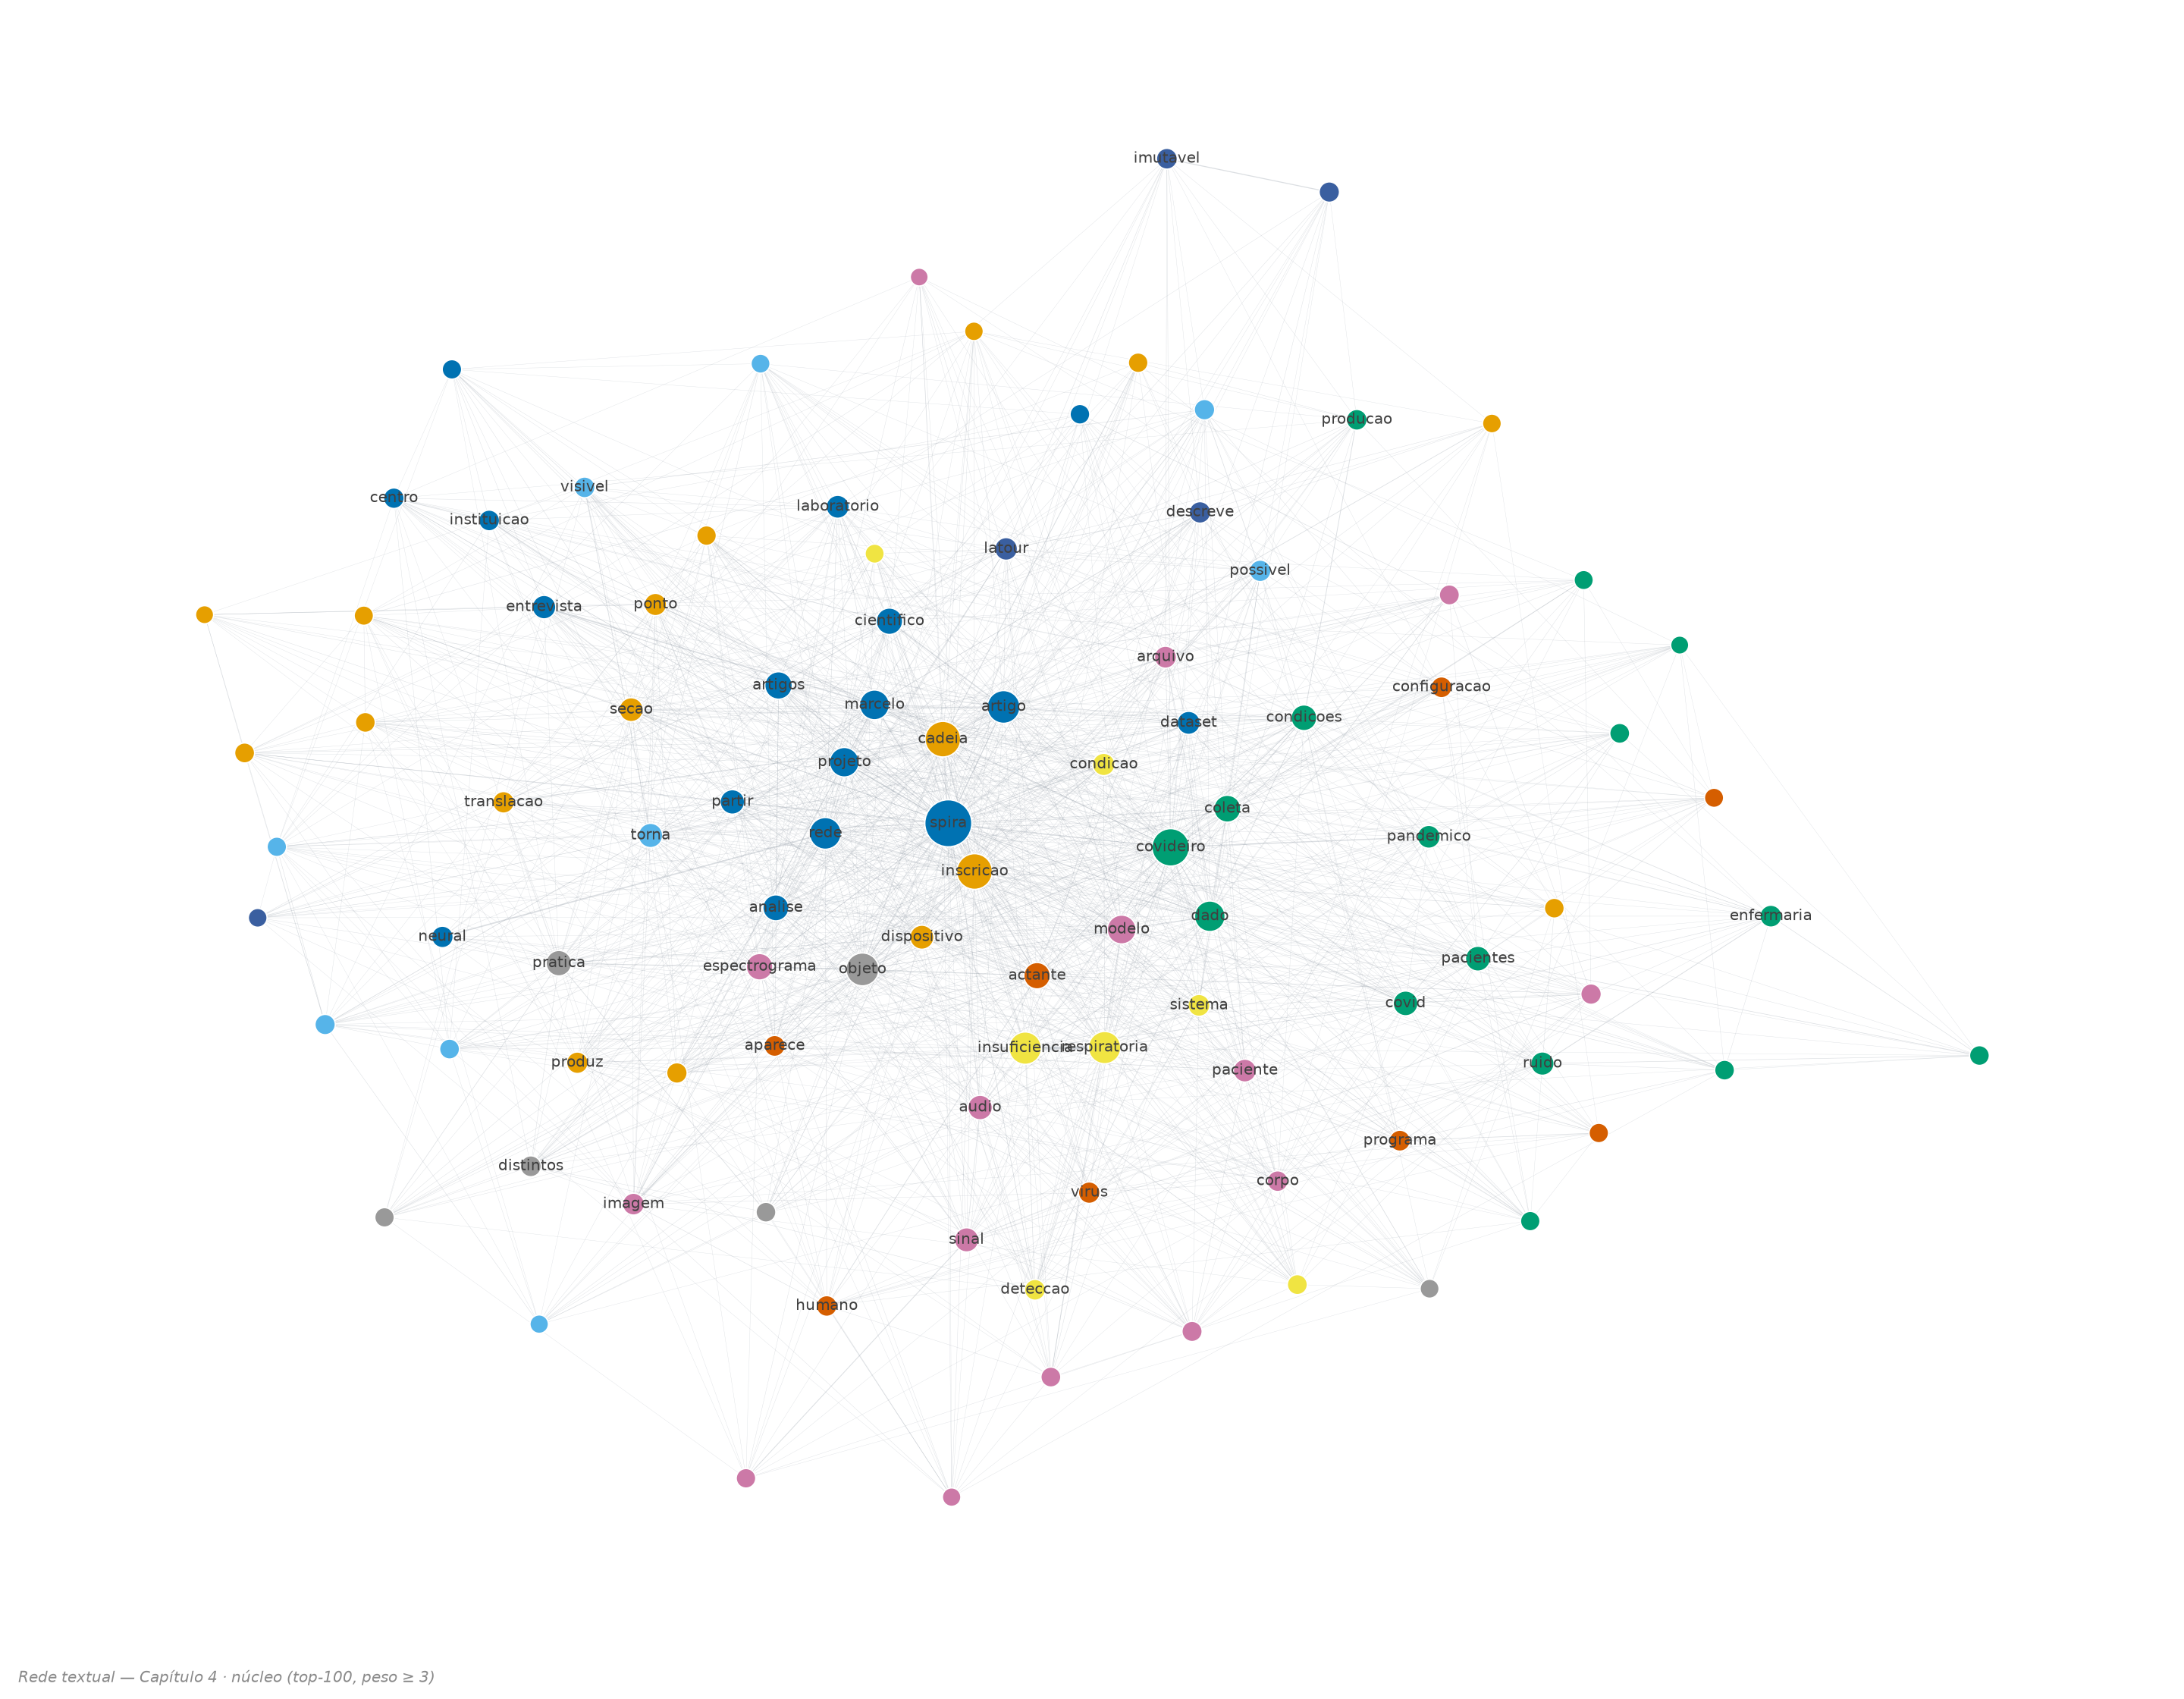
\includegraphics[width=1.0\textwidth,keepaspectratio]{figuras/cap.4/infranodus_cap4_focus.png}
\caption[Núcleo da rede textual do capítulo~\ref{capitulo4} (análise de rede textual)]{Núcleo da rede textual do capítulo~\ref{capitulo4} (análise de rede textual). Os nós são os 100 termos com maior \textit{degree} ponderado; o tamanho do nó é proporcional ao \textit{degree}; a cor indica a comunidade detectada por Louvain ponderado; arestas com peso $\geq 3$. Comparada à figura~\ref{fig:infranodus-cap4-network}, esta vista retém apenas o esqueleto semântico do capítulo, ou seja, os conceitos mais centrais e suas conexões fortes, sem a periferia. Versão de alta resolução, arquivo \texttt{.gexf} para o \texttt{Gephi} e relatório completo disponíveis em \texttt{infranodus/} no repositório \url{https://github.com/julianehelanski/tecno-etnografia-centro-ia}.}
\label{fig:infranodus-cap4-focus}
\end{figure}

\begin{figure}[!htb]
\centering
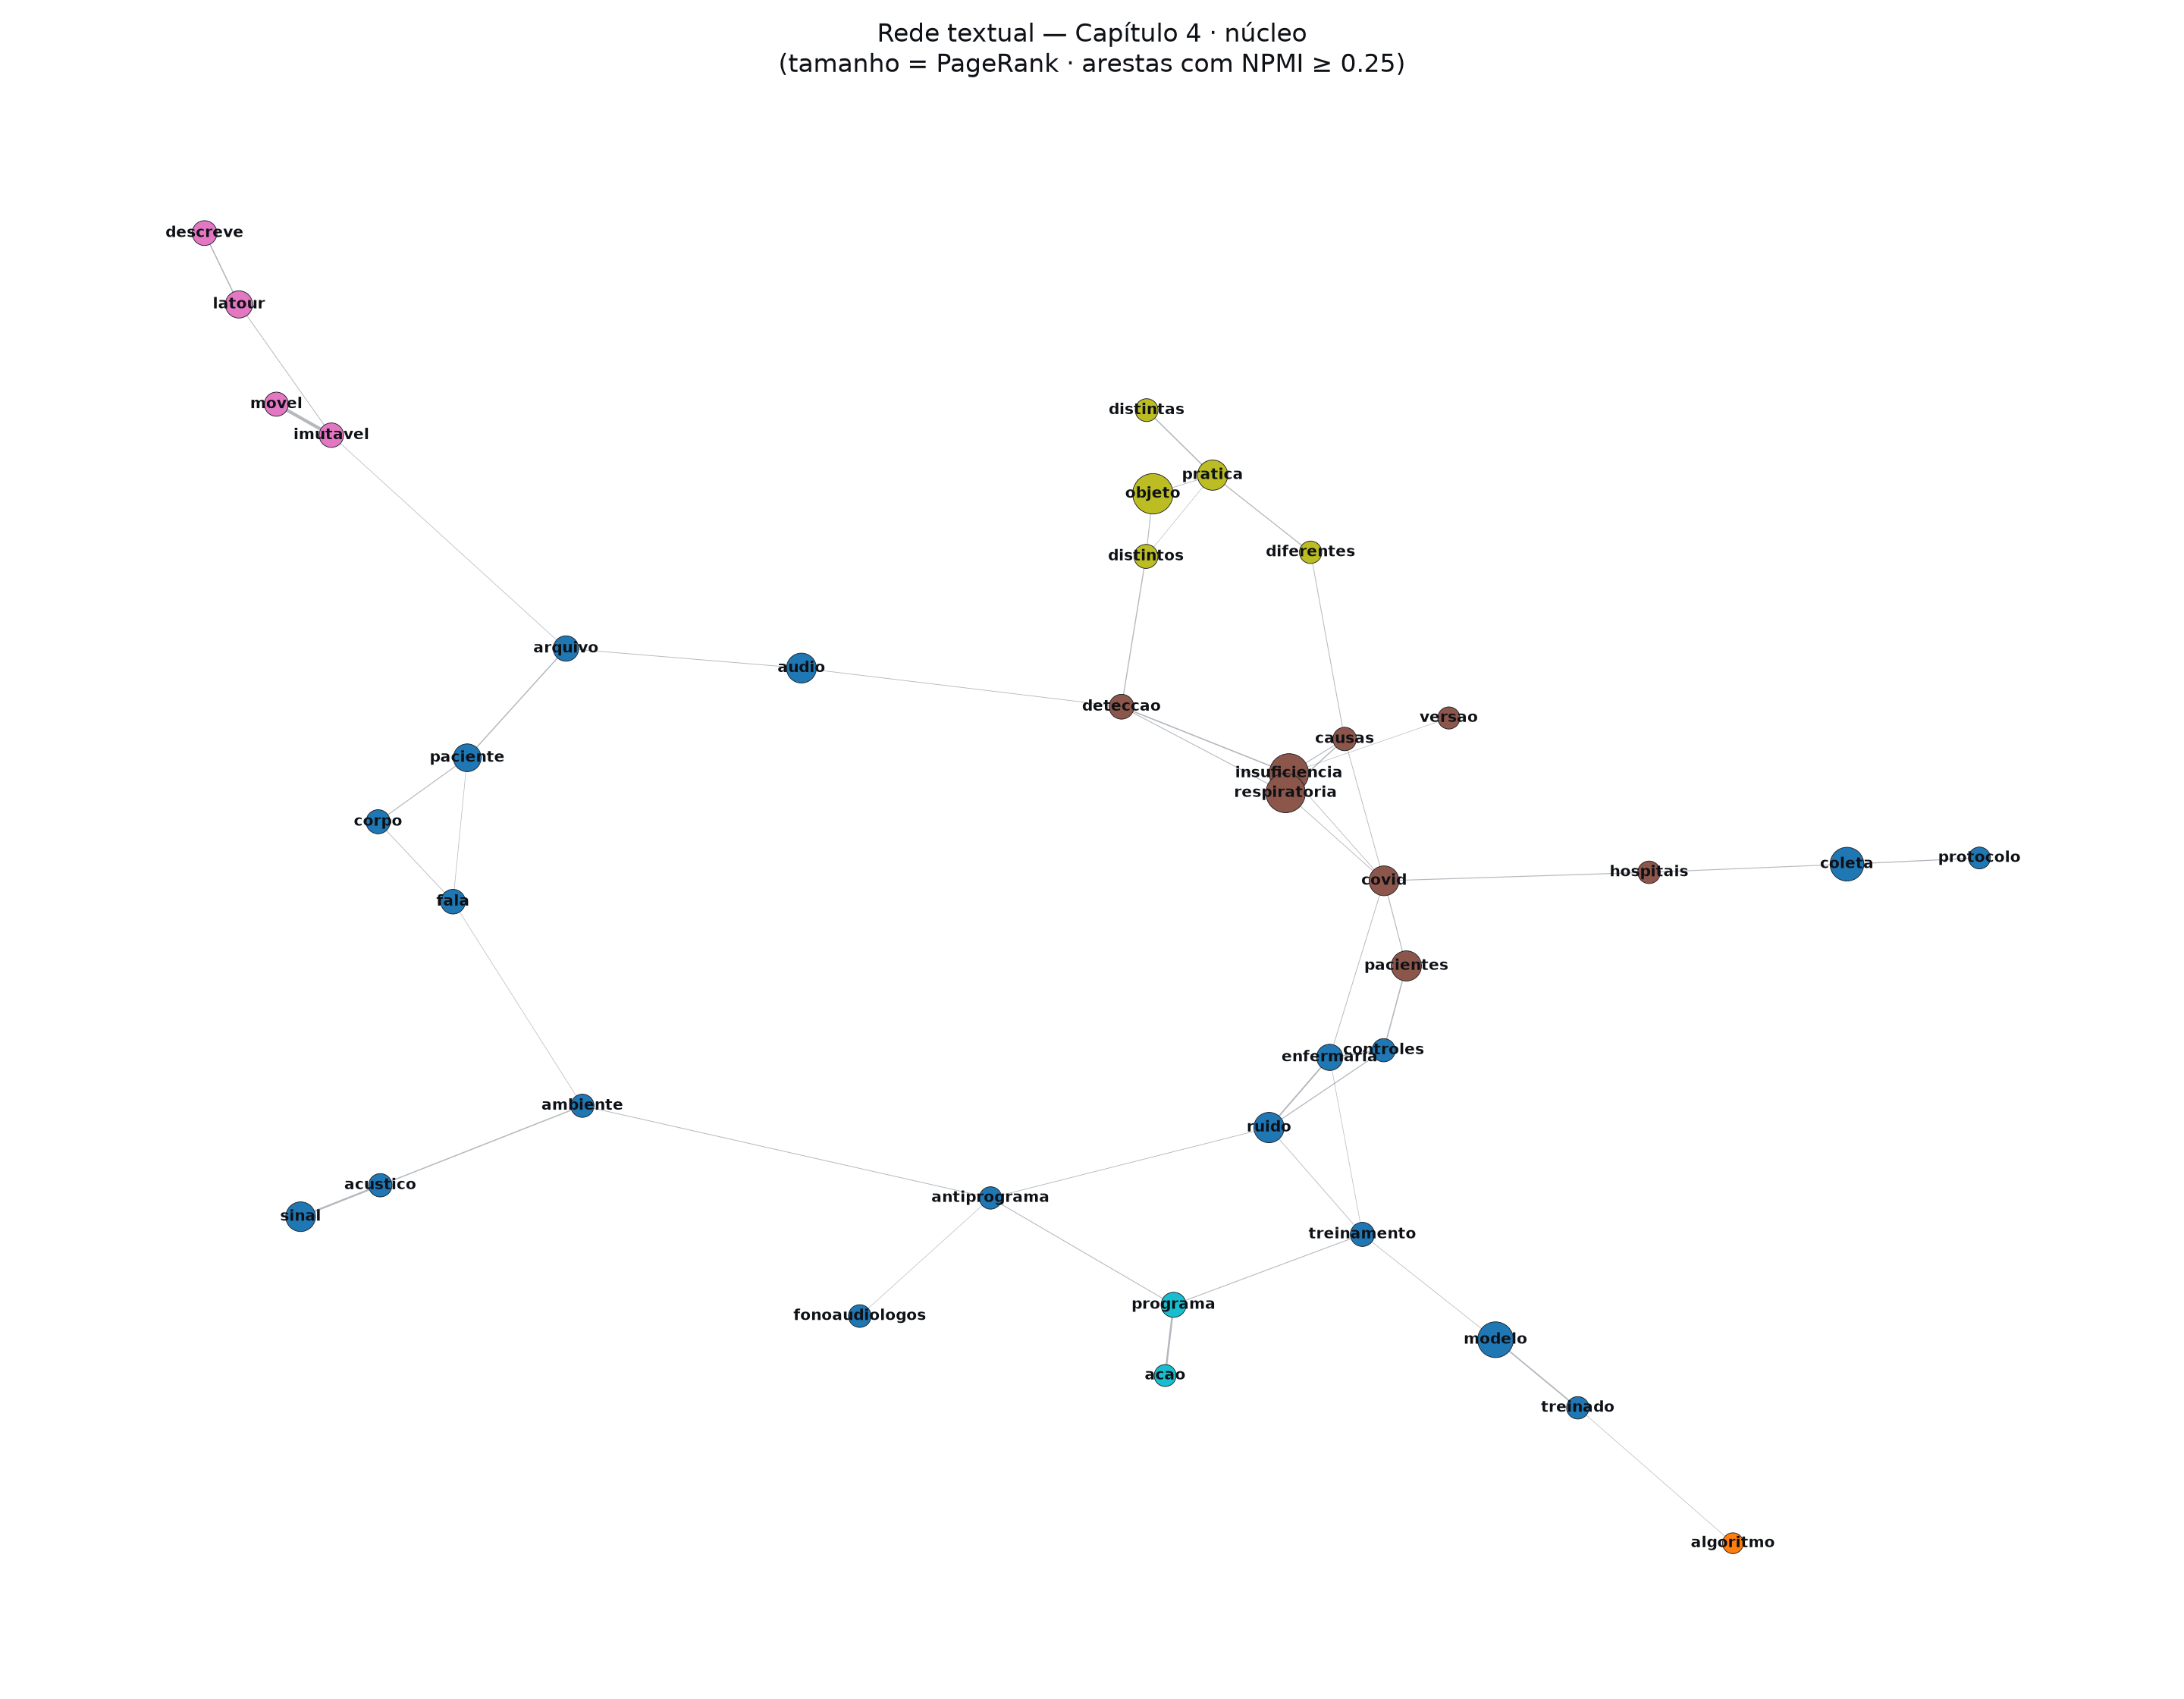
\includegraphics[width=1.0\textwidth,keepaspectratio]{figuras/cap.4/infranodus_cap4_focus_pmi.png}
\caption[Núcleo da rede textual do capítulo~\ref{capitulo4} ponderado por PageRank e NPMI]{Núcleo da rede textual do capítulo~\ref{capitulo4}, ranqueado por critérios informacionais em vez de frequentistas. Os mesmos 100 nós da figura~\ref{fig:infranodus-cap4-focus} são exibidos, mas o tamanho passa a ser proporcional ao \textit{PageRank} (centralidade na rede, em vez de contagem bruta) e as arestas são filtradas pelo \textit{Normalized Pointwise Mutual Information} (NPMI~$\geq 0{,}25$), retendo apenas co-ocorrências surpreendentes dadas as frequências marginais de cada termo. A cor mantém a comunidade Louvain. Esta vista promove conceitos pouco frequentes e estrategicamente posicionados, e deprime termos onipresentes cuja associação com qualquer outro é trivial, funcionando como contraponto à leitura puramente frequentista. Métricas e arquivo \texttt{.gexf} em \texttt{infranodus/} no repositório \url{https://github.com/julianehelanski/tecno-etnografia-centro-ia}.}
\label{fig:infranodus-cap4-pmi}
\end{figure}

\begin{figure}[!htb]
\centering
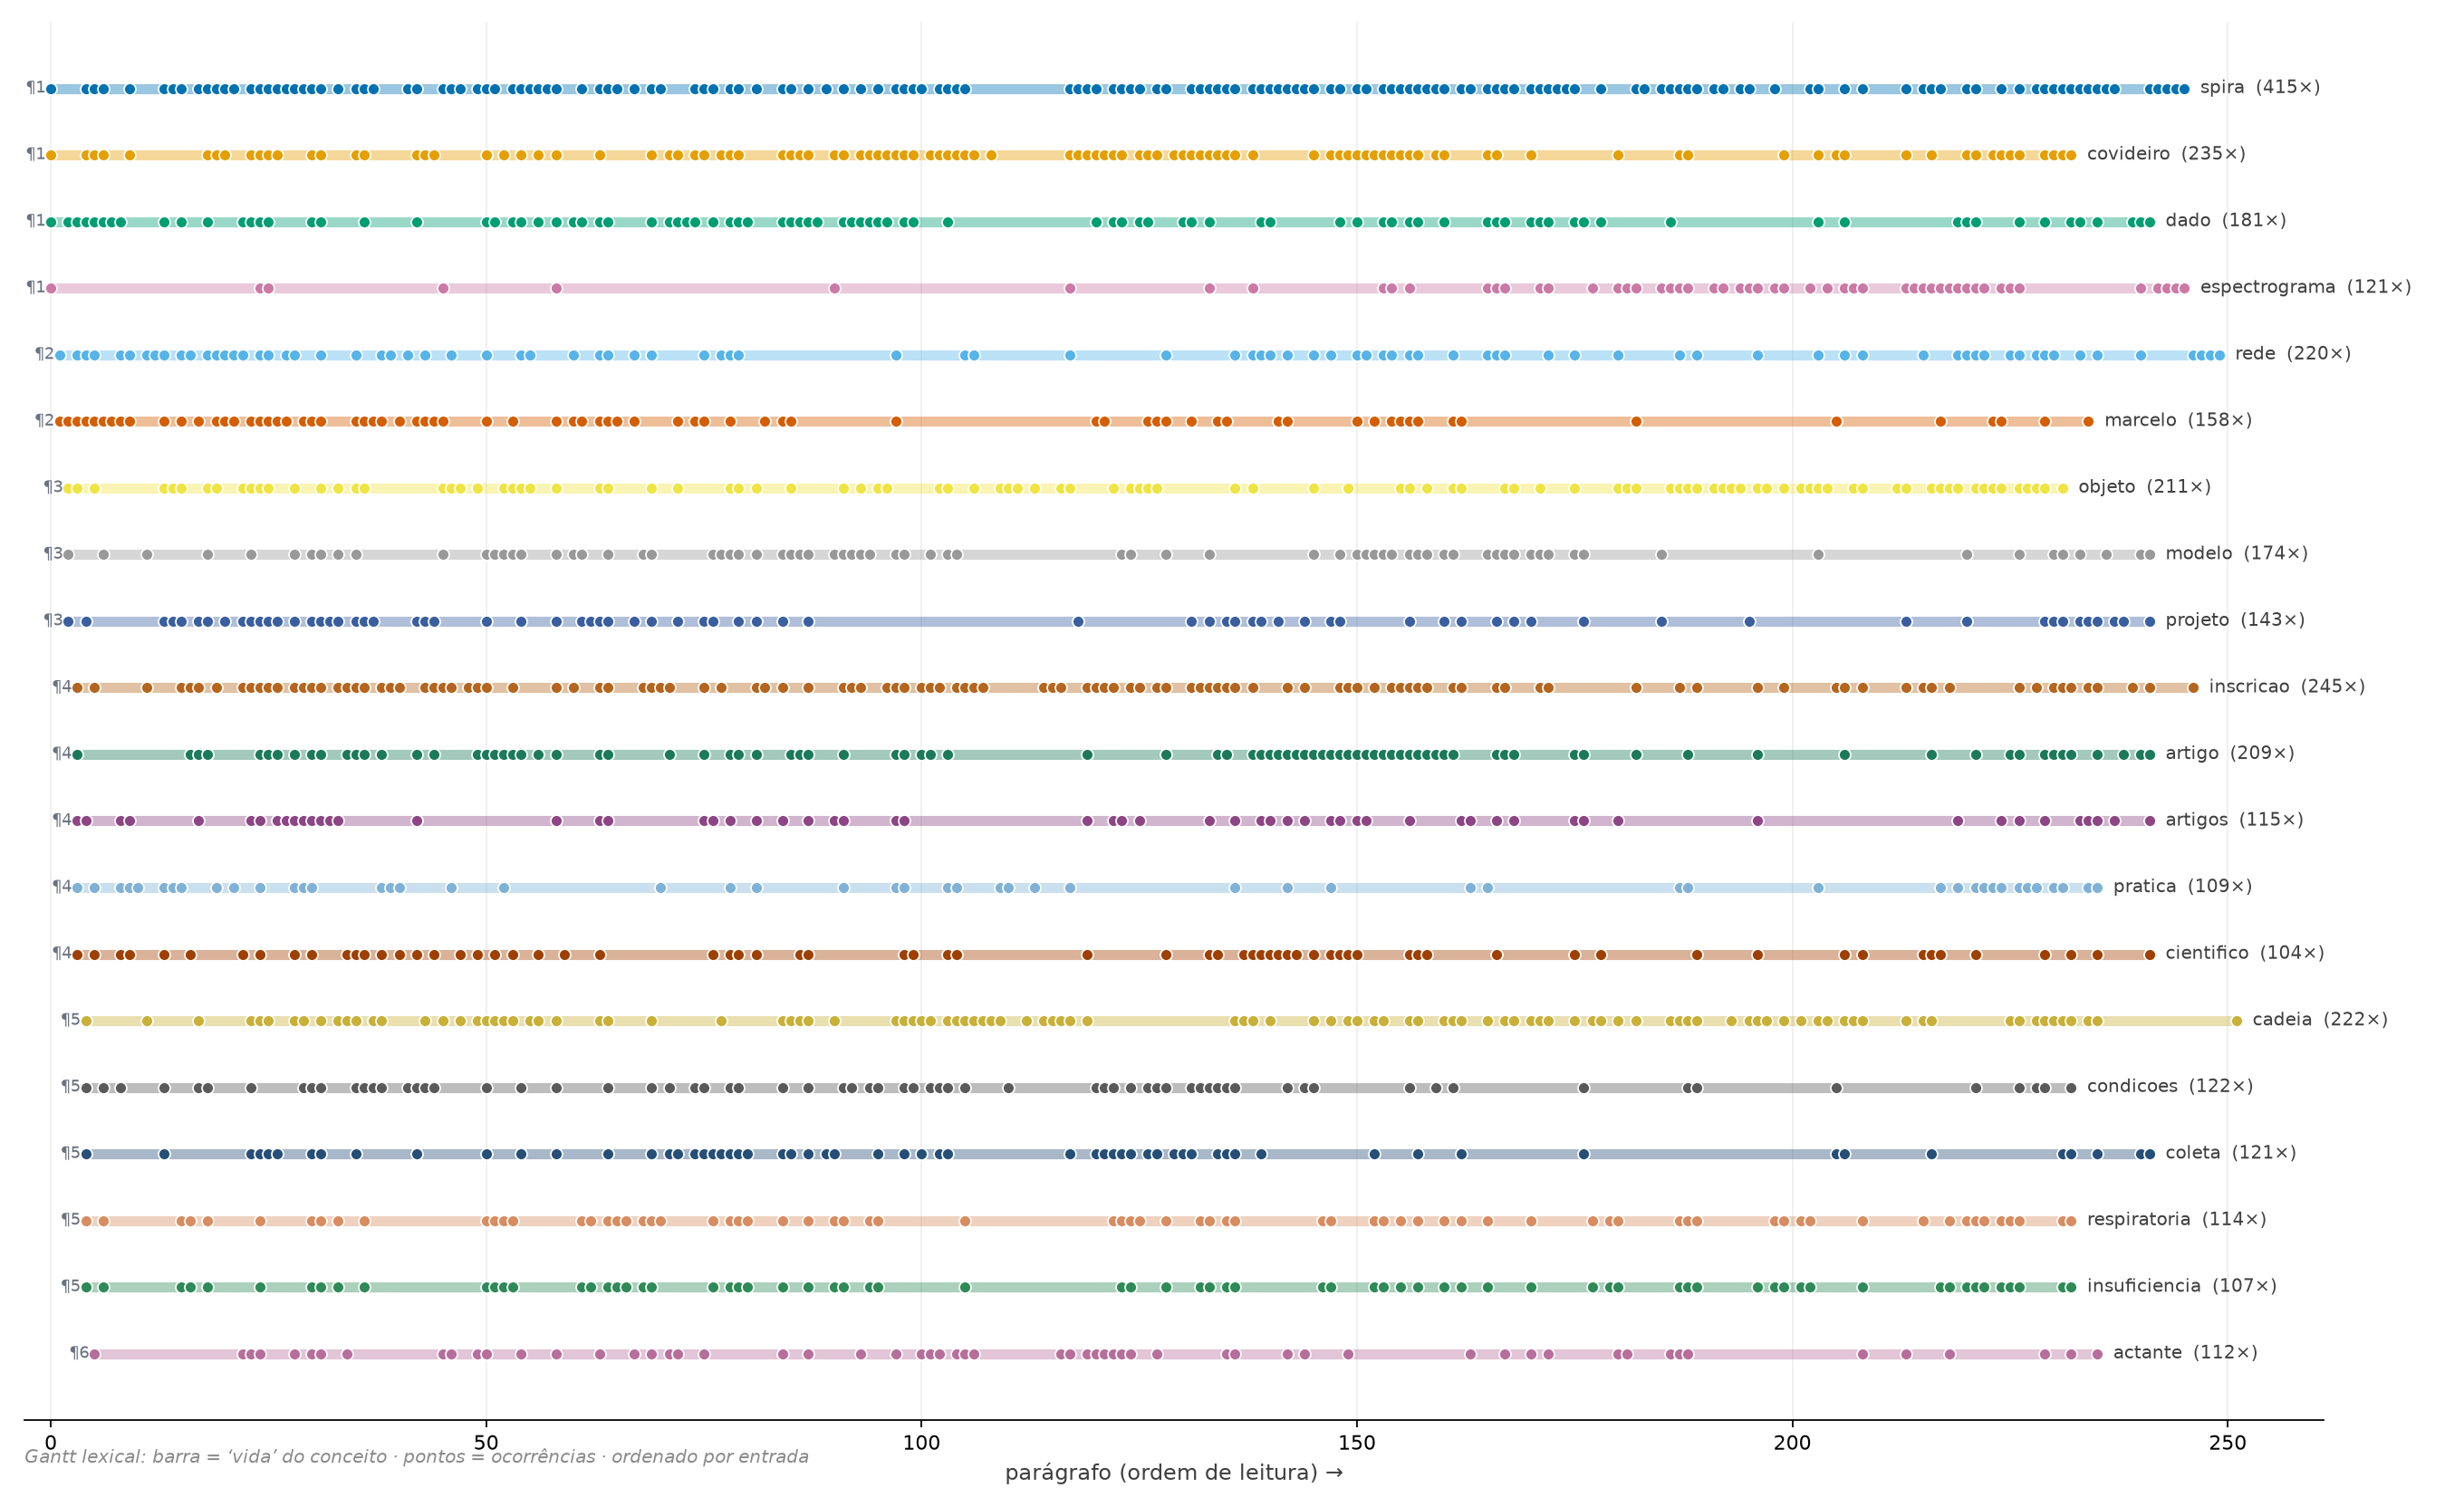
\includegraphics[width=1.0\textwidth,keepaspectratio]{figuras/cap.4/trajectory_gantt.png}
\caption[Gantt lexical do capítulo~\ref{capitulo4}: entrada, persistência e saída dos conceitos]{Gantt lexical do capítulo~\ref{capitulo4}. Cada linha corresponde a um dos 20 conceitos de maior frequência, excluídos termos genéricos e o marcador \texttt{claude}; o eixo horizontal é a ordem de leitura em parágrafos. A barra colorida marca a vida do conceito no capítulo, do parágrafo de primeira aparição (rótulo \P\textit{n}) ao último; os pontos sobre a barra indicam cada ocorrência; o número entre parênteses à direita é a contagem total. As linhas estão ordenadas por parágrafo de entrada, evidenciando a sequência em que cada noção é convocada e por quanto tempo permanece em circulação. Gerado pelo \textit{script} \texttt{narrative\_trajectory.py}, disponível em \url{https://github.com/julianehelanski/tecno-etnografia-centro-ia/tree/main/infranodus}.}
\label{fig:trajectory-cap4-gantt}
\end{figure}

\begin{figure}[!htb]
\centering
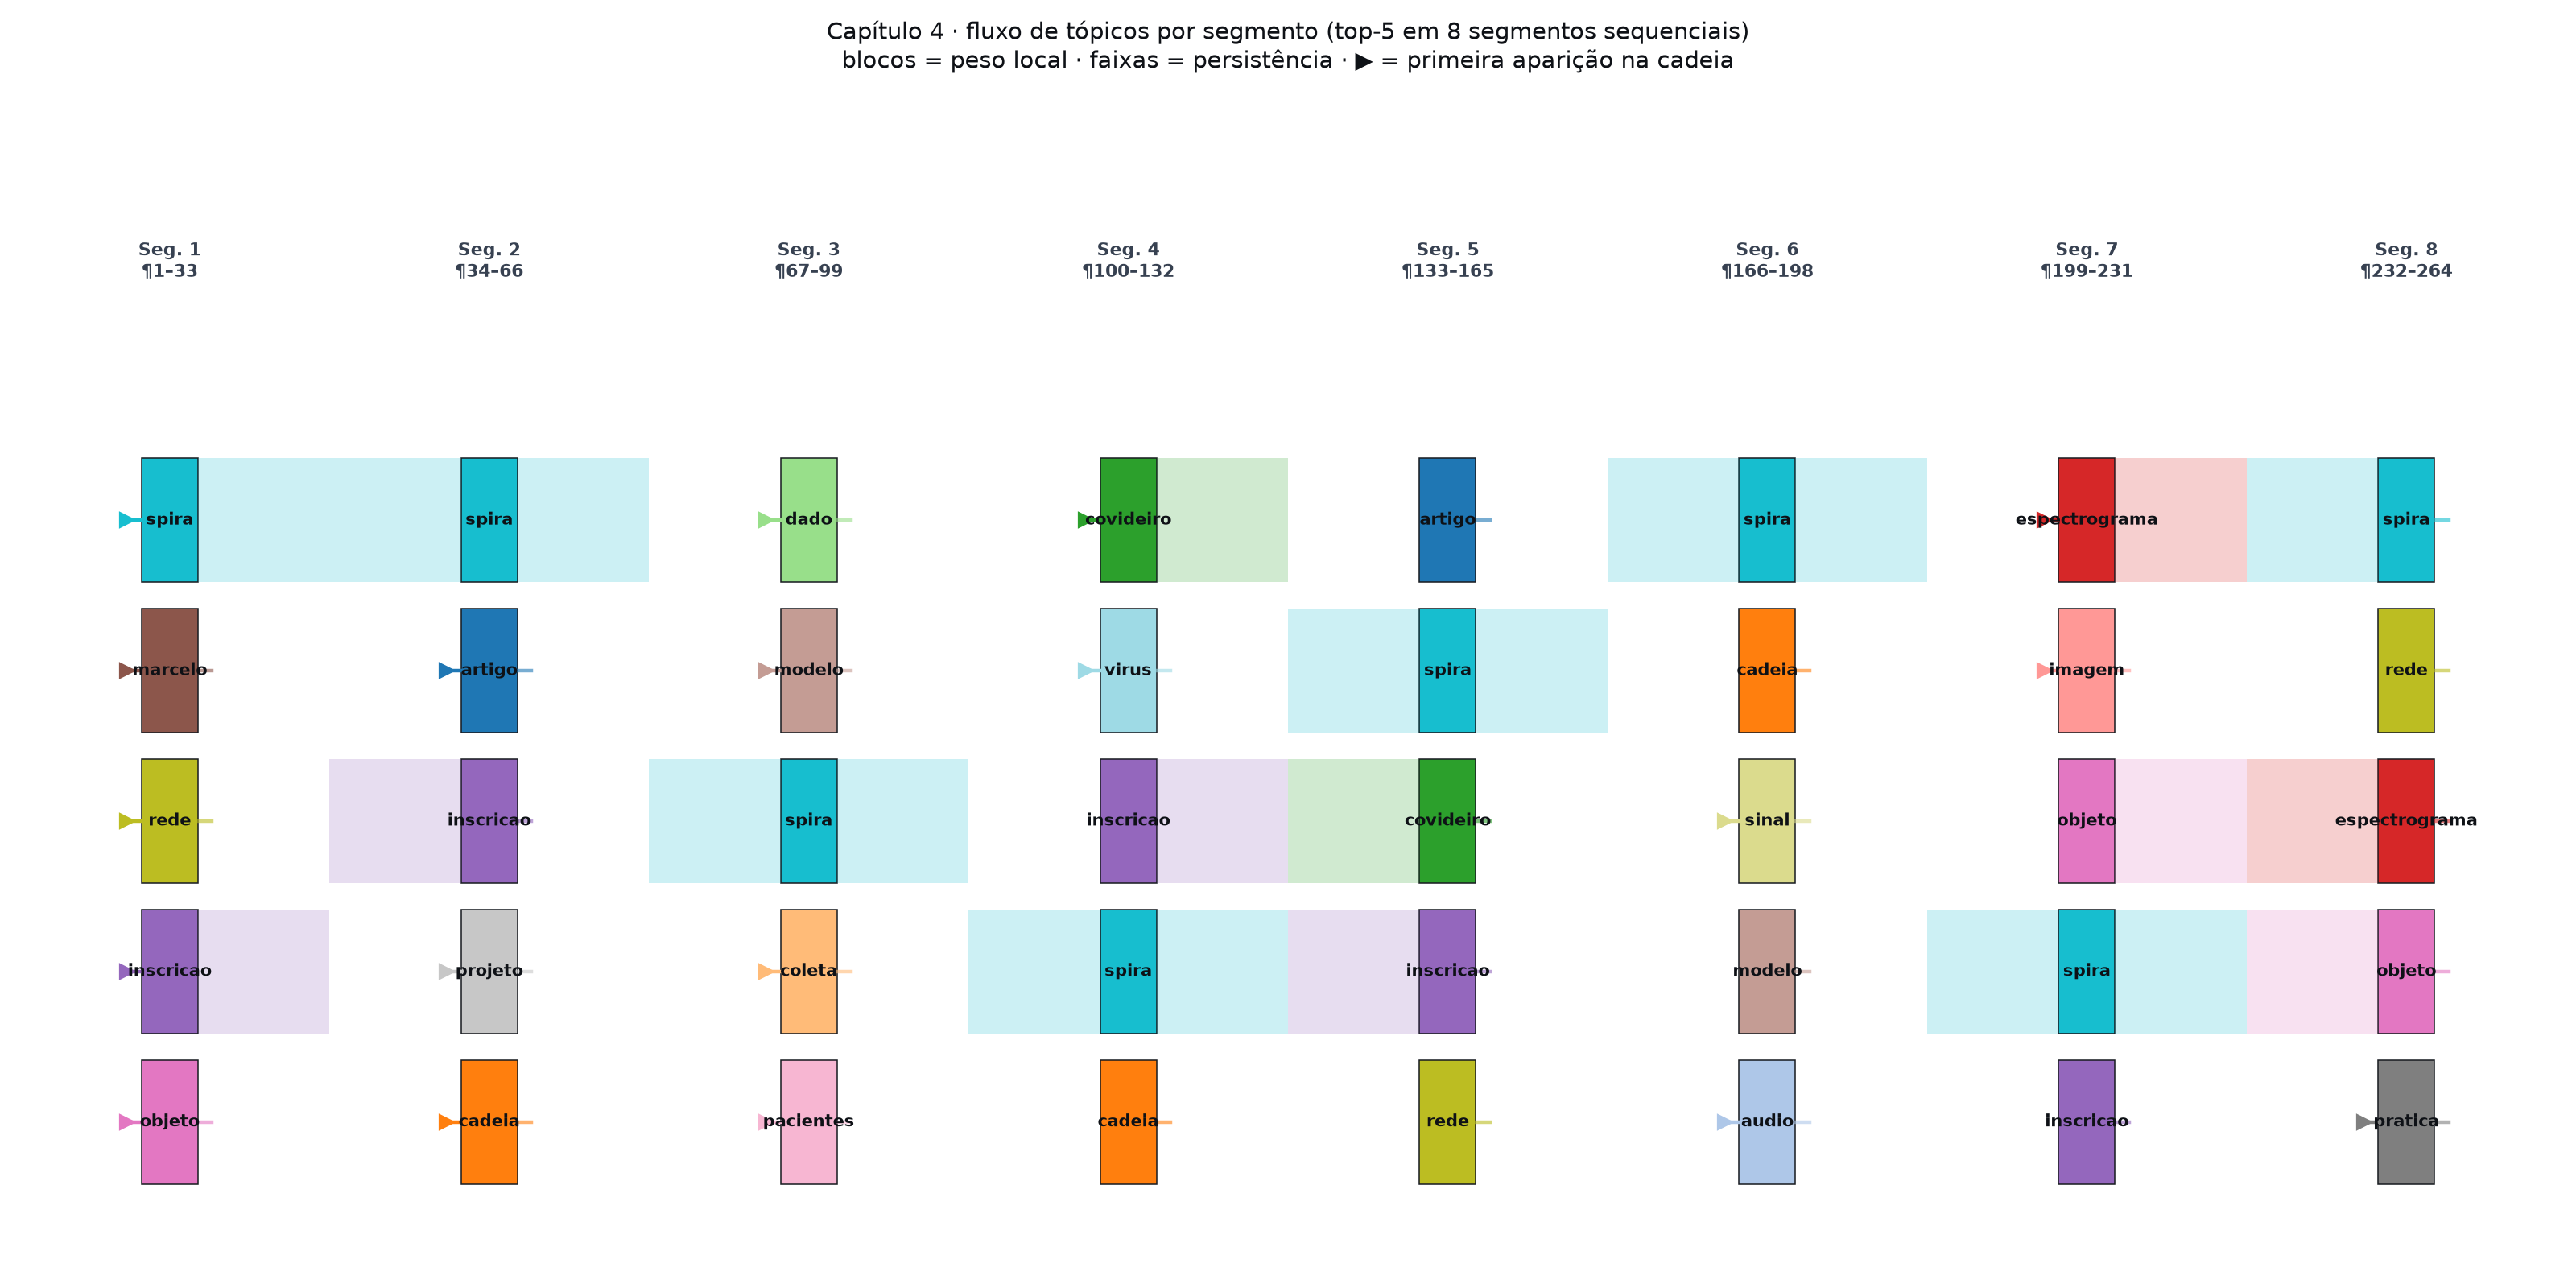
\includegraphics[width=1.0\textwidth,keepaspectratio]{figuras/cap.4/trajectory_alluvial.png}
\caption[Fluxo aluvial de tópicos ao longo do capítulo~\ref{capitulo4}]{Fluxo aluvial do capítulo~\ref{capitulo4}. O capítulo é particionado em 8 segmentos sequenciais de igual extensão em parágrafos (rótulos \P\textit{n}--\P\textit{m} no topo); em cada segmento são listados os 5 termos de maior frequência local (blocos coloridos, com a posição vertical refletindo o \textit{ranking} dentro do segmento). Faixas translúcidas conectam um termo a si mesmo entre segmentos adjacentes quando ele persiste no \textit{top}-5, materializando continuidades temáticas; setas $\blacktriangleright$ assinalam a primeira aparição de um conceito na cadeia. A figura responde à pergunta \enquote{o que se liga a quê ao longo do capítulo} e torna visíveis tanto os tópicos persistentes quanto as entradas tardias e saídas precoces. Gerado pelo \textit{script} \texttt{narrative\_trajectory.py}, disponível em \url{https://github.com/julianehelanski/tecno-etnografia-centro-ia/tree/main/infranodus}.}
\label{fig:trajectory-cap4-alluvial}
\end{figure}

\begin{figure}[!htb]
\centering
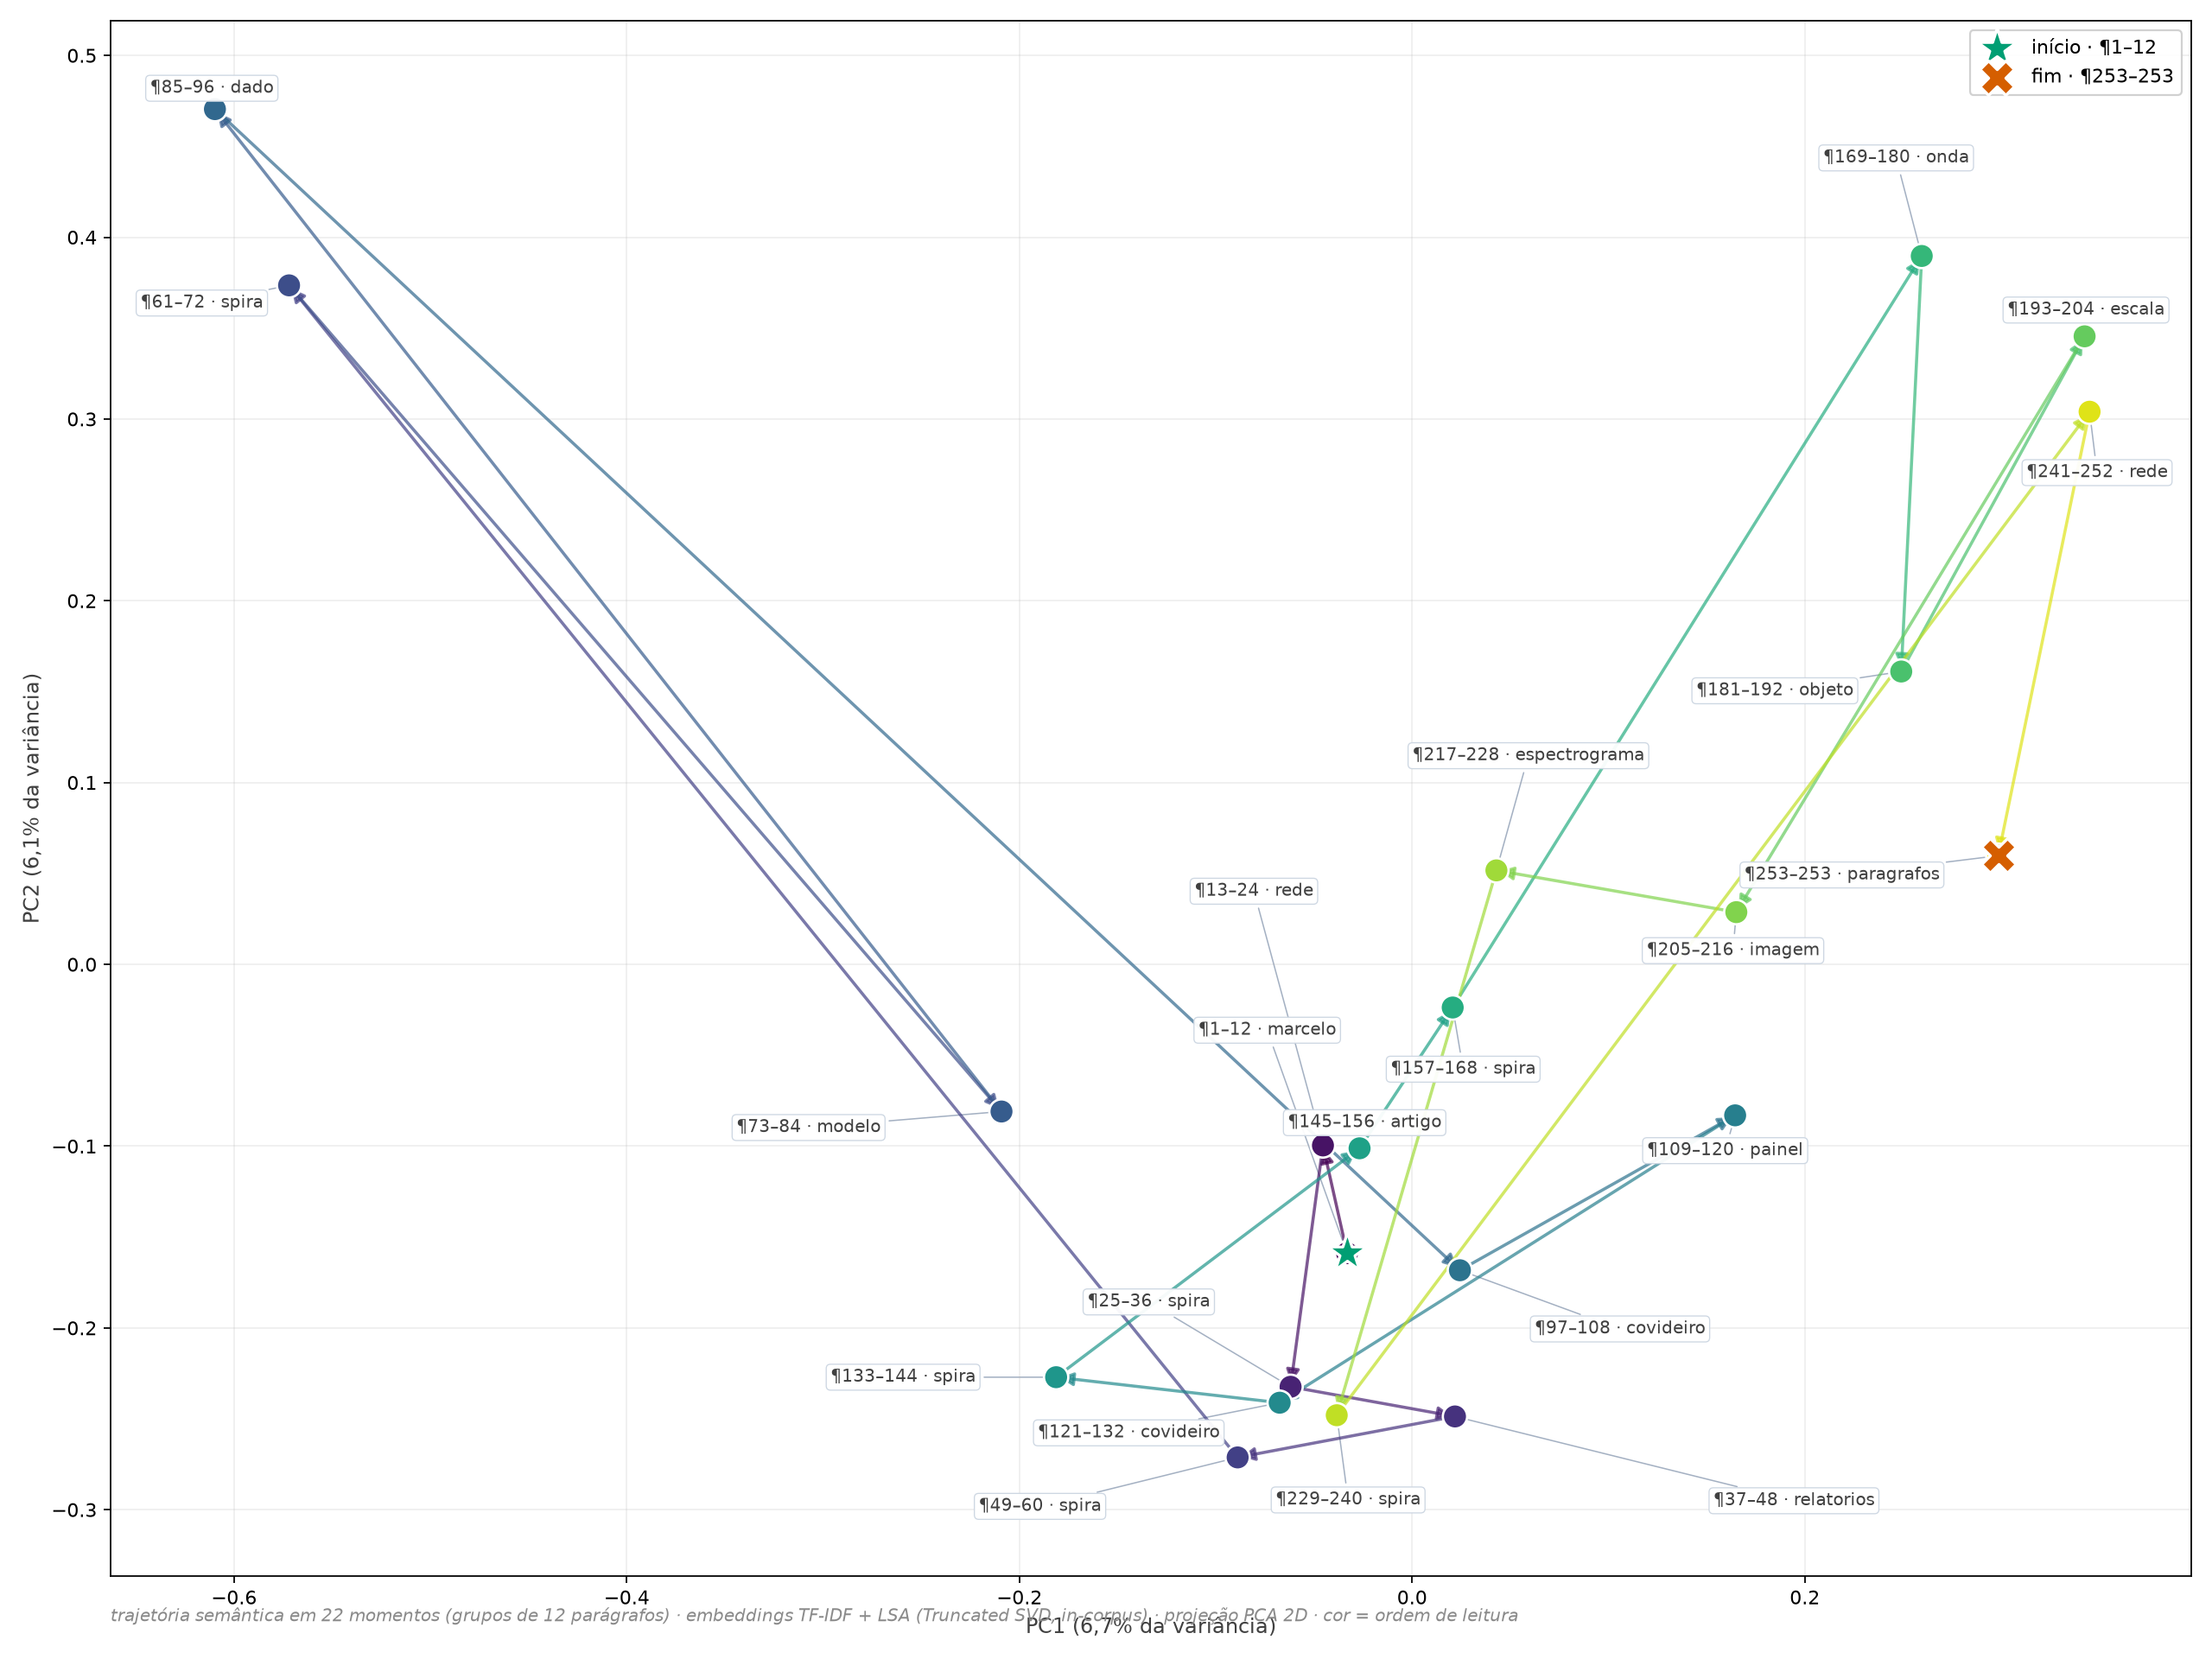
\includegraphics[width=1.0\textwidth,keepaspectratio]{figuras/cap.4/trajectory_semantic.png}
\caption[Trajetória semântica do capítulo~\ref{capitulo4}]{Trajetória semântica do capítulo~\ref{capitulo4}. Os parágrafos são agrupados em \textit{momentos} de 5 parágrafos consecutivos; cada momento é vetorizado por \textit{TF-IDF} (unigramas e bigramas) seguido de redução por \textit{Truncated SVD} (\textit{Latent Semantic Analysis} \textit{in-corpus}, \textit{fallback} usado quando o \textit{sentence-transformer} multilíngue não está disponível) e projetado em duas dimensões por PCA. Cada ponto é um momento, rotulado com o intervalo de parágrafos e o termo dominante; as setas seguem a ordem de leitura, com gradiente \textit{viridis} do início ($\star$ verde) ao fim ($\times$ vermelho). Distâncias no plano aproximam dissimilaridade lexical entre momentos; deslocamentos longos indicam mudanças temáticas, voltas curtas indicam retomada de campo semântico já visitado. O percentual de variância explicada por cada eixo aparece nos rótulos. Gerado pelo \textit{script} \texttt{narrative\_trajectory.py}, disponível em \url{https://github.com/julianehelanski/tecno-etnografia-centro-ia/tree/main/infranodus}.}
\label{fig:trajectory-cap4-semantic}
\end{figure}
\chapter{Conclusão}
\chapter{Considerações finais}
\label{capitulo5}

Uma dimensão atravessa os cinco registros analíticos e pede ênfase antes do fechamento do capítulo: os mecanismos documentados aqui agem através dos arranjos que governaram (e deixaram de governar) o vínculo. Isso significa que a análise se dirige aos arranjos, não às pessoas que os ocuparam. Fábio e Cláudio demonstraram, ao longo das entrevistas, reflexividade sobre tensões, conhecimento dos ciclos de negócio da \texttt{IBM} e compromisso com excelência científica e interesse público. Quando Cláudio descreveu o projeto de línguas indígenas como exemplo de \textit{AI for Good} que \enquote{vai virar algum dia produto... jamais. E não se espera que vire} (PINHANEZ, 2025, informação verbal), ele articulou uma valorização da pesquisa com impacto social irredutível à lógica comercial. Quando Fábio insistiu que \enquote{a gente não faz nenhum projeto para a IBM} (COZMAN, 2025, informação verbal), articulou sua experiência concreta de autonomia acadêmica, confirmada pelo fato de o \texttt{C4AI} produzir, ao longo de cinco anos, \textit{datasets} abertos, publicações em conferências internacionais e ferramentas disponibilizadas sob licenças permissivas.

A coexistência entre essa autonomia declarada e as reorientações documentadas da agenda não configura contradição. Partes em qualquer colaboração influenciam mutuamente suas prioridades, e, quando a translação funciona, essa influência é experimentada como colaborativa mais do que como coerção \parencite{Latour2011CienciaEmAcao}. A dificuldade é que a translação bem-sucedida tende ao que Latour chama de \textit{black-boxing}, isto é, as negociações e os diferenciais de poder que deram forma ao arranjo tornam-se invisíveis. A ausência de arranjos explícitos de governança no \texttt{C4AI} significou que essas dinâmicas de translação se deram informalmente, sem procedimentos documentados que tornassem rastreável o processo decisório. Sem mecanismos institucionais que garantissem a rastreabilidade, é impossível verificar se os interesses foram de fato negociados ou se o alinhamento refletiu capacidade assimétrica de definir o benefício compartilhado.

Callon, Lascoumes e Barthe formulam, em sua análise de \enquote{democracia técnica}, que as assimetrias consequentes raramente decorrem da conduta de atores individuais \parencite{Callon2011Acting}. Elas decorrem de arranjos sociotécnicos que distribuem de forma desigual capacidades, recursos e poder de definição das agendas. No caso do \texttt{C4AI}, o que estreitava de antemão as escolhas possíveis inclui o subfinanciamento crônico da pesquisa pública brasileira, a dependência de recursos corporativos para infraestrutura computacional considerada básica, as pressões institucionais por \textit{impacto} e \textit{inovação} definidos em termos que valem também em registros corporativos, e as assimetrias geopolíticas que fazem da mão de obra qualificada brasileira, na formulação de Cláudio, \enquote{barata demais} em comparações internacionais. Neste espaço, as decisões de aceitar ou recusar financiamento corporativo, publicar em \textit{open access} ou em periódicos fechados, colaborar ou não com pesquisadores \texttt{IBM}, ocorrem dentro de margens estreitas. Como Fábio observou ao explicar por que projetos em saúde e agronegócio permaneceram ativos mesmo após a \texttt{IBM} reorientar os interesses: \enquote{a gente sempre mantém uma certa independência porque a gente tem recursos da Fapesp} (COZMAN, 2025, informação verbal). Projetos que deixaram de ser de interesse da \texttt{IBM} continuaram com recursos da \texttt{FAPESP}. Essa \enquote{certa independência} parcial e constantemente renegociada é o espaço real de agência disponível para pesquisadores em contextos periféricos do Sul Global.

Ao documentar essas dinâmicas, este capítulo não propõe que arranjos público-privados sejam intrinsecamente problemáticos nem que toda colaboração com corporações configure captura disfarçada. Os centros derivados, os pesquisadores formados e os \textit{datasets} abertos são contribuições verificáveis para a capacidade brasileira em IA. Os cinco registros indicam, contudo, que acordos apresentados como horizontais e mutuamente benéficos podem obscurecer assimetrias estruturais de poder, de recursos e de capacidade de definir os termos da colaboração quando a governança permanece informal. O \texttt{C4AI}, nesse registro, é uma existência parcial no sentido em que a Lição~2 do Capítulo~\ref{capitulo1} formula a partir de Strathern: conectado simultaneamente à autonomia acadêmica e à racionalidade corporativa sem ser redutível a nenhuma das duas. A \texttt{IBM} foi, ao mesmo tempo, constitutiva e periférica à pesquisa que financiou. Fábio e Cláudio foram, ao mesmo tempo, atores da universidade pública e porta-vozes de um arranjo corporativo. Os grupos de pesquisa foram ao mesmo tempo do \texttt{C4AI} e não eram, como mostra a trajetória dos centros derivados que partilharam a origem e deixaram de compartilhar o vínculo. É também aqui que se resolve a tensão que anunciei na abertura, quando disse que tomar a \texttt{IBM} como objeto experimentava, na prática, o esforço de fazer alianças sem ferir os sentimentos estabelecidos, no sentido de Stengers. Dirigir a análise aos arranjos, e não às pessoas que os ocuparam, é o que me permitiu descrever criticamente a rede da qual eu também era parte sem converter Fábio e Cláudio em réus: a aliança que mantive com eles e com o centro não se desfez ao descrever as assimetrias, porque a crítica recaiu sobre os dispositivos de governança que faltaram, e não sobre quem agiu dentro das margens estreitas que esses dispositivos deixavam. Foi esse o modo que encontrei de honrar a confiança que me foi dada sem abrir mão da descrição que me propus a fazer.

Recolho esses fios. Este capítulo documentou um arranjo público-privado em inteligência artificial desde a constituição em outubro de 2020 até o encerramento em dezembro de 2025, ao enredar dois horizontes temporais. No horizonte recente, a etnografia acompanhou quase quatro anos de funcionamento do \texttt{C4AI} como acordo entre \texttt{USP}, \texttt{FAPESP} e \texttt{IBM}, até a comunicação interna de não-renovação em agosto de 2025 e a dissolução pública entre novembro e dezembro do mesmo ano. No horizonte de mais de um século, a trajetória rastreou 135 anos de estratégias \texttt{IBM} de construção de dependências tecnológicas, da tabulação de Hollerith no Censo dos EUA de 1890 aos ecossistemas contemporâneos de IA cognitiva. Os cinco registros analíticos que sistematizei, a assimetria orçamentária, a multiplicação institucional, a reorientação sistemática da agenda, a seletividade geográfica e o arranjo que não se inscreveu, descrevem padrões observáveis do arranjo que emergem do seguir dos atores.

A incubação bem-sucedida do \texttt{C4AI}, em sua ambivalência, atravessa todo o caso. Pelo que se costuma contar como sucesso, o \texttt{C4AI} funcionou: múltiplos centros catalisados, \textit{datasets} liberados sob licenças permissivas, centenas de estudantes formados, publicações em conferências internacionais, reconhecimento no terceiro Fórum Global da UNESCO sobre Ética em Inteligência Artificial em Bangkok, em junho de 2025 \parencite{C4AI2025}. O arranjo, ainda assim, foi encerrado. A multiplicação que o sustentava criou as próprias condições do encerramento: os centros derivados asseguraram financiamento autônomo, e, a partir desse ponto, o incentivo corporativo para sustentar o investimento original diminuiu. De uma perspectiva, a \enquote{missão} se cumpriu: o acordo construiu capacidade duradoura. De outra, a mesma evidência põe em jogo a sustentabilidade do vínculo e a ausência de planejamento de transições. As duas leituras incidem sobre a mesma cadeia de associações que o capítulo rastreou.

A clareza maior que este capítulo entrega está naquilo que os arranjos não registravam. A \texttt{IBM} seguiu as provisões contratuais existentes e estava formalmente no direito de não renovar. O que permanece é que as provisões nunca responderam às perguntas elementares sobre o propósito da colaboração, os critérios para sua continuação e os procedimentos de transição. A parte pública comprometeu-se com desenvolvimento institucional de longo prazo, ao passo que a parte corporativa reteve flexibilidade para ajustar compromissos. Pesquisadores brasileiros em regime de bolsa, trabalhando fora das proteções laborais convencionais, enfrentaram dificuldades particulares durante a transição. Essas dinâmicas produzem efeitos que arranjos de governança formalizados teriam condições de antecipar.

A articulação da estratégia de \enquote{ecossistema} que observei na \textit{bluetalks} indica que os porta-vozes corporativos agiam com clareza sobre a posição que ocupavam. A parte pública, ao longo dos cinco anos, moveu-se dentro de um arranjo cujos dispositivos escritos não registravam os termos que o encerramento viria a tornar urgentes. A descrição desses registros de ausência, o descompasso entre horizontes temporais, a concentração de fontes, a invisibilidade do processo decisório sobre reorientações, a condição dos bolsistas, a dependência infraestrutural e epistêmica, a opacidade da consulta estratégica, foi reunida na seção~\ref{subsec:arranjo_nao_inscreveu}.

A seletividade geográfica tensiona os limites do que a etnografia pode estabelecer. A \texttt{IBM} concluiu suas atividades no Brasil simultaneamente à manutenção e à expansão de iniciativas na Índia (Hybrid Cloud Lab com o IISc em 2021, Quantum Valley Tech Park com a TCS e o governo de Andhra Pradesh em maio de 2025, BharatGen em setembro de 2025) e nos EUA (Genesis Mission em novembro de 2025). Fatores comparativos de escala, tamanho de mercado e prioridades estratégicas provavelmente influenciaram essas decisões, e os pesos específicos permanecem indisponíveis. O que o arranjo não inscreveu aparece aqui como opacidade, condição de funcionamento que atravessa a confiança e o planejamento de todas as partes.

O que descrevi aqui, no plano institucional, ainda não responde por completo à pergunta etnográfica que levantei no Capítulo~\ref{capitulo1}: onde e como pesquisadores fazem IA no cotidiano? Como se materializaram, durante os cinco anos de funcionamento do \texttt{C4AI}, as dependências infraestruturais e as assimetrias geopolíticas que identifiquei aqui? Como os pesquisadores negociaram algoritmos, dados, infraestruturas computacionais limitadas e demandas institucionais em tensão? O próximo capítulo examina essas perguntas pelo sítio etnográfico do desenvolvimento do \texttt{Spira} durante a pandemia de Covid-19, um dos projetos ativos durante o período de vigência do arranjo. Acompanho Marcelo Finger e os múltiplos actantes que se reuniram na construção de IA preditiva em contexto de urgência sanitária. Trata-se de mudar de ponto de entrada, porque a rede não tem topo nem fundo, e a passagem ao próximo capítulo não desce de um nível superior a um inferior: parto dos arranjos institucionais e das trajetórias históricas para as práticas cotidianas e as translações situadas, outro ponto da mesma rede a partir do qual outras associações se tornam seguíveis. O que aparece, desse outro ponto, é que fazer inteligência artificial no Brasil daquele período foi trabalho situado, material e político, atravessado pelas mesmas dependências estruturais que identifiquei aqui, e negociado de formas criativas pelos pesquisadores no dia a dia do laboratório.

Em dezembro de 2025, quando encerrei a redação deste capítulo, a rede estava em reconfiguração. O que permanecia em jogo para os actantes que restavam no centro era a redistribuição dos recursos, das competências e dos vínculos institucionais que o arranjo havia organizado por cinco anos: o financiamento da \texttt{FAPESP}, a infraestrutura computacional do JAIRU recém-inaugurado, os grupos que haviam conquistado autonomia e os que permaneciam dependentes dos recursos conjuntos, e as relações com as corporações que poderiam ou não suceder o papel exercido pela \texttt{IBM}. Nenhum desses elementos estava definido no momento em que esta escrita se encerrou. As conversas informais com Fábio e Cláudio naquele período registravam interpretações ainda abertas, antes que a narrativa definitiva sobre o que havia acontecido se fechasse. A encruzilhada, nos termos de Latour, é o ponto em que os porta-vozes ainda não sabem com quantos atores falam \parencite{Latour2011CienciaEmAcao}. É exatamente aí que esta etnografia encerrou o registro.

Volto, antes de encerrar, às perguntas com que abri este capítulo, para dizer o que o seguir dos atores me deixou afirmar sobre cada uma, sem fechá-las em respostas. Perguntei por quais modos uma corporação passa a extrair valor de suas conexões com universidades: o que pude descrever foi um conjunto de modos rastreáveis, a aprendizagem barata que Cláudio nomeou, a multiplicação de centros que a atividade do \texttt{C4AI} catalisou, a reorientação da agenda conforme as frentes corporativas se deslocavam, sem que eu possa fixar, a partir do que segui, a intenção que teria guiado cada movimento. Perguntei o que significa \enquote{fortalecer um ecossistema de IA}: vi esse fortalecimento e a atuação comercial da própria \texttt{IBM} correrem juntos, e descrevi essa coincidência sem precisar atribuir à empresa o cálculo de fazer um gerar o outro. Perguntei de que maneira se \enquote{descobre} um modelo de negócios baseado em código aberto e como essa descoberta orienta políticas globais: rastreei a fala de Cláudio sobre os anos 1990 e a aquisição da Red Hat até uma trajetória mais longa, em que a abertura técnica e o fechamento infraestrutural se sustentam mutuamente, sem que a fala comprove a trajetória nem a trajetória comprove a fala. E perguntei como tudo isso se relaciona com um centro de IA numa universidade pública brasileira: o \texttt{C4AI} apareceu como o ponto em que essas racionalidades se inscreveram localmente, sob a forma de um arranjo que se compôs com facilidade e se desfez com a mesma facilidade que o instrumento de 2016 já previa. As perguntas que permaneceram abertas não se fecharam por falta de rastreamento; elas tocam no que corre por canais que não acompanhei, e é dessa fronteira que trato a seguir.

Retomo, para encerrar, a pergunta que a \textit{bluetalks} me deu e que tomei como questão deste capítulo: o que circula nessas cadeias, por quais caminhos e sob que termos. A circulação de valor que pude descrever é a que passa pelos porta-vozes que segui e pelos documentos que pude consultar. O que corre por canais privados, os cálculos internos, as negociações bilaterais e as deliberações estratégicas, não se ofereceu à descrição, e é esse o ponto que prefiro não suavizar: a opacidade do núcleo decisório é parte do que circula nessas cadeias e condição de seu funcionamento, e não uma falha do meu rastreamento. Foi o corte que fiz ao seguir os porta-vozes, no sentido de \textcite{strathern2011cortando}, que me deu a circulação institucional e me subtraiu a decisória, e descrever esse corte como tal, em vez de simular um acesso que não tive, é o que mantém a descrição honesta quanto ao que a minha posição alcança. Segui os atores como Latour recomenda \parencite{Latour2011CienciaEmAcao} e documentei aquilo que escolheram tornar visível, ciente de que o que permanece invisível molda os desfechos de forma substantiva. O que este capítulo entrega, então, é a descrição do que age informalmente nos arranjos que produziu, e da visibilidade que o encerramento lançou sobre essa informalidade. O que o caso não resolve, e que a evidência etnográfica por si só não tem condições de resolver, é uma pergunta sobre o papel que resta à universidade quando a fronteira da produção de conhecimento em IA migra para a infraestrutura corporativa. Se os vínculos com quem comanda essa infraestrutura se tornaram condição de funcionamento para a pesquisa brasileira em IA, a pergunta é sob quais arranjos eles vêm sendo buscados, com quais salvaguardas, e em direção a quais finalidades. A essa pergunta não entrego uma conclusão; ofereço um problema que a descrição tornou visível. É esse problema que o próximo capítulo, ao descer para o cotidiano do \texttt{Spira}, ajuda a recolocar desde dentro do laboratório.
Retomo, para encerrar, a pergunta que a \textit{bluetalks} me deu e que tomei como questão deste capítulo: o que circula nessas cadeias, por quais caminhos e sob que termos. A circulação de valor que pude descrever é a que passa pelos porta-vozes que segui e pelos documentos que pude consultar. O que corre por canais privados, os cálculos internos, as negociações bilaterais e as deliberações estratégicas, não se ofereceu à descrição, e é esse o ponto que prefiro não suavizar: a opacidade do núcleo decisório é parte do que circula nessas cadeias e condição de seu funcionamento, e não uma falha do meu rastreamento. Foi o corte que fiz ao seguir os porta-vozes, no sentido de \textcite{strathern2011cortando}, que me deu a circulação institucional e me subtraiu a decisória, e descrever esse corte como tal, em vez de simular um acesso que não tive, é o que mantém a descrição honesta quanto ao que a minha posição alcança. Segui os atores como Latour recomenda \parencite{Latour2011CienciaEmAcao} e documentei aquilo que escolheram tornar visível, ciente de que o que permanece invisível molda os desfechos de forma substantiva. O que este capítulo entrega, então, é a descrição do que age informalmente nos arranjos que produziu, e da visibilidade que o encerramento lançou sobre essa informalidade. O que o caso não resolve, e que a evidência etnográfica por si só não tem condições de resolver, é uma pergunta sobre o papel que resta à universidade quando a fronteira da produção de conhecimento em IA migra para a infraestrutura corporativa. Se os vínculos com quem comanda essa infraestrutura se tornaram condição de funcionamento para a pesquisa brasileira em IA, a pergunta é sob quais arranjos eles vêm sendo buscados, com quais salvaguardas, e em direção a quais finalidades. A essa pergunta não entrego uma conclusão; ofereço um problema que a descrição tornou visível. É esse problema que o próximo capítulo, ao descer para o cotidiano do \texttt{Spira}, ajuda a recolocar desde dentro do laboratório.
   % Conclusões

%%%%%%%%%%%%%%%%%%%%%%%%%% REFERÊNCIAS %%%%%%%%%%%%%%%%%%%%%%%%%%
\clearpage
\phantomsection
\addcontentsline{toc}{chapter}{Referências}
\printbibliography[title=Referências]

%%%%%%%%%%%%%%%%%%%%%%%%%% APÊNDICES %%%%%%%%%%%%%%%%%%%%%%%%%%
%\appendix
%\chapter*{Glossário\markboth{Glossário}{}}  % \markboth{}{} é utilizado para corrigir o cabeçalho.
 \label{glossario:latour}
\addcontentsline{toc}{chapter}{Glossário}
\begin{description}

\noindent Este glossário reúne os conceitos de Bruno Latour, Latour e Woolgar, Annemarie Mol e John Law mobilizados ao longo desta tese. As entradas não pretendem fixar definições canônicas; expõem, antes, o uso analítico que cada conceito recebe nos capítulos em que aparece. As referências remetem às edições consultadas.

\bigskip

%% ────────────────────────────────────────────────────────────────────
\section*{Actante}
\addcontentsline{toc}{section}{Actante}
Termo tomado da semiótica greimasiana e reapropriado por Latour para designar qualquer entidade, humana ou não humana, que age ou tem sua ação representada em uma rede. Um actante é definido pragmaticamente: sua identidade emerge da lista de ações e reações que apresenta quando submetido a provas de força, e não de qualidades intrínsecas previamente fixadas \parencite[p.~127]{Latour2011CienciaEmAcao}. Nesta tese, o conceito permite tratar no mesmo plano analítico pesquisadores, GPUs, algoritmos, contratos institucionais, vozes gravadas em enfermarias e o próprio vírus SARS-CoV-2 (Capítulos 1 e 4). A simetria metodológica exigida pelo conceito é seu aspecto mais exigente: não se pode recorrer a fatores sociais ou naturais preestabelecidos para explicar o desfecho de controvérsias; é preciso observar empiricamente quem ou o que age em cada situação.

\bigskip

%% ────────────────────────────────────────────────────────────────────
\section*{Agência dos textos científicos e funil de interesses}
\addcontentsline{toc}{section}{Agência dos textos científicos e funil de interesses}

Law, em \textit{Laboratories and Texts} \parencite{Law1986Laboratories}, argumenta que o texto científico opera como operador de translação que inscreve seus leitores, conduzindo-os ao longo de um caminho especificado. A força de um artigo não reside apenas em sua lógica interna, mas em sua capacidade de mobilizar elementos heterogêneos, dados, instituições, conceitos e especialistas, para impor uma estrutura ao mundo e exercer influência à distância. É por isso que Law descreve o texto como ``a arma secreta da ciência'': transportável, durável e estruturado, o artigo pode circular além do laboratório e agir sobre leitores que nunca estiveram presentes nas práticas que o produziram \parencite{Law1986Laboratories}. O conceito de \textit{funil de interesses} descreve a estrutura pela qual o artigo começa com um problema amplo para atrair o maior público possível e estreita progressivamente o alcance à medida que direciona o leitor em direção a um conjunto particular de pontos. As referências bibliográficas operam como \textit{interessements} elementares: interpõem forças entre o leitor e sua indiferença ao artigo, emprestando a autoridade de outros atores-rede para conduzi-lo adiante. Callon articula a mecânica do \textit{interessement} textual ao demonstrar que o artigo científico, como o laboratório, reúne forças numa combinação que pode escapar ao controle, e que a solução é dispor as palavras em configuração adequada por meio de uma série de \textit{interessements} encadeados \parencite[pp.~71--72]{Callon1986Mapping}. No Capítulo 4, esse vocabulário é aplicado ao artigo do SPIRA: as tabelas de acurácia, as curvas ROC e a seção de materiais e métodos são analisadas como dispositivos que constroem ``realidade'' por encadeamento de inscrições que tornam progressivamente mais difícil ao leitor contestar o resultado sem dominar as mesmas ferramentas que o produziram \parencite{Law1986Laboratories,Callon1986Mapping}.

\bigskip

%% ────────────────────────────────────────────────────────────────────
\section*{Aliados e alistamento de aliados}
\addcontentsline{toc}{section}{Aliados e alistamento de aliados}

Fazer ciência, para Latour, é o processo de recrutar e estabilizar aliados cada vez mais numerosos e heterogêneos: instrumentos, colegas, financiadores, artigos anteriores, dados, instituições e públicos. A força de uma alegação científica depende menos de sua relação com a Natureza do que da extensão da rede que a sustenta: ``aqueles que não alistaram ninguém são ninguém'' \parencite[p.~239]{Latour2011CienciaEmAcao}. Referências bibliográficas funcionam, nessa lógica, como exército de reforços que o autor mobiliza para tornar o custo da discordância proibitivo \parencite[p.~53]{Latour2011CienciaEmAcao}. No Capítulo 2, o próprio processo de construção do referencial teórico desta tese é narrado como alistamento retrospectivo de aliados em resposta a problemas empíricos. Nos Capítulos 3 e 4, o conceito orienta a análise das alianças que Fábio, Cláudio e Marcelo constroem com IBM, FAPESP, hospitais, pacientes e algoritmos para sustentar a pesquisa em IA.

\bigskip

%% ────────────────────────────────────────────────────────────────────
\section*{Caixa-preta}
\addcontentsline{toc}{section}{Caixa-preta}

Quando um fato científico ou um artefato técnico se estabiliza a ponto de não mais suscitar controvérsias sobre seu funcionamento ou conteúdo, diz-se que ele foi posto em caixa-preta. A expressão, oriunda da cibernética, designa o ponto em que uma afirmação ou dispositivo pode ser utilizado como insumo por outros atores sem que seus pressupostos precisem ser reabertos. Latour formula a Regra 1 de método a partir dessa imagem: estudar a ciência em ação significa chegar antes que fatos e máquinas se tenham transformado em caixas-pretas, ou acompanhar as controvérsias que as reabrem \parencite[p.~420]{Latour2011CienciaEmAcao}. No Capítulo 4, o SPIRA é caracterizado como ciência em construção: o artigo científico estabilizou parcialmente os resultados como imutável móvel, mas a falha de generalização para além dos dados pandêmicos impediu que o sistema alcançasse o estatuto de caixa-preta plenamente fechada.

\bigskip

%% ────────────────────────────────────────────────────────────────────
\section*{Centro de cálculo}
\addcontentsline{toc}{section}{Centro de cálculo}

Ponto de acumulação e combinação de inscrições provenientes de locais distantes. Latour mostra que o poder de alguns atores sobre outros resulta de sua capacidade de reunir, comparar e mobilizar representações de fenômenos que ocorrem em outros pontos da rede. O laboratório científico é um centro de cálculo paradigmático: converte entidades do mundo (amostras, medições, observações) em inscrições combináveis que podem ser comparadas, sobrepostas e enviadas a outros centros \parencite{Latour1990Drawing}. No Capítulo 4, o covideiro funciona como centro de cálculo distribuído e precário: enfermarias, smartphones e hospitais convertem vozes humanas em arquivos de áudio que chegam ao IME-USP para transformação em coeficientes MFCC e, finalmente, em classificações binárias de insuficiência respiratória.

\bigskip

%% ────────────────────────────────────────────────────────────────────
\section*{Ciência em ação e ciência pronta (a imagem de Janus)}
\addcontentsline{toc}{section}{Ciência em ação e ciência pronta (a imagem de Janus)}

Latour propõe a imagem do deus romano Janus, que possui dois rostos voltados a direções opostas, para distinguir dois modos de apresentação da ciência. A ciência pronta é a que aparece nos artigos publicados e nos manuais: resultados estabilizados, fatos consolidados, caixas-pretas fechadas, retórica depurada. A ciência em ação é aquela que se observa antes da estabilização: controvérsias abertas, aliados em disputa, instrumentos que falham, dados que não se encaixam, negociações em andamento \parencite[cap.~1]{Latour2011CienciaEmAcao}. O subtítulo desta tese, \textit{como seguir cientistas e engenheiros universidade afora}, é variação direta do subtítulo de \textit{Ciência em ação} e sinaliza a escolha metodológica de observar o segundo rosto de Janus. O SPIRA é analisado no Capítulo 4 precisamente como ciência em construção: o artigo publicado exibe o rosto da ciência pronta (96,5\% de acurácia); a etnografia do covideiro expõe o rosto da ciência em ação (fonoaudiólogos que abandonaram, ruídos que saturaram o sinal, modelos que não generalizaram).

\bigskip

%% ────────────────────────────────────────────────────────────────────
\section*{Controvérsia}
\addcontentsline{toc}{section}{Controvérsia}

Situação em que a validade de um fato científico ou o funcionamento de um artefato técnico ainda está em disputa entre grupos de atores. Para Latour, as controvérsias são as janelas metodológicas por excelência: é nelas que se torna visível o trabalho de construção que a ciência pronta subsequentemente apaga \parencite[cap.~2]{Latour2011CienciaEmAcao}. Acompanhar controvérsias equivale a acompanhar ciência em ação. Na Regra 3, Latour adverte que a resolução de uma controvérsia é a causa da representação da Natureza, e não sua consequência: não se pode invocar a Natureza para explicar por que uma disputa foi encerrada desse modo. No Capítulo 4, a limitação de generalização do SPIRA mantém aberta uma controvérsia técnica: os modelos treinados com dados de COVID-19 não se aplicam bem a insuficiências respiratórias de outras etiologias, e essa abertura é analisada como evidência da dependência do sistema em relação às condições que o produziram.

\bigskip

%% ────────────────────────────────────────────────────────────────────
\section*{Enactment e multiplicidade ontológica}
\addcontentsline{toc}{section}{Enactment e multiplicidade ontológica}

Mol, em \textit{The Body Multiple} \parencite{mol2002body}, propõe uma ruptura com a epistemologia da representação ao demonstrar que práticas distintas não observam o mesmo objeto de perspectivas diferentes, mas produzem objetos ontologicamente distintos. A aterosclerose da sala de cirurgia, do laboratório de patologia e da consulta ambulatorial não são versões de uma mesma doença; são objetos diferentes, \textit{enacted} (performados) por práticas irredutíveis entre si. Como Mol formula: ``realidade não precede as práticas mundanas nas quais interagimos com ela, mas é moldada dentro dessas práticas'' \parencite[p.~6]{mol2002body}. O \textit{enactment} designa esse processo pelo qual práticas produzem objetos sem que haja um objeto singular preexistente a ser representado. A multiplicidade resultante é coexistência de realidades parcialmente conectadas entre si, e não pluralidade de perspectivas sobre uma realidade única. No Capítulo 4, o conceito é mobilizado para descrever a insuficiência respiratória do SPIRA: a IR do covideiro (escuta clínica incorporada), a IR do oxímetro (saturação como número) e a IR do classificador binário (pausa acústica computacionalmente codificada) são enactuações distintas que coexistem sem convergir em um objeto único. A tentativa do SPIRA de estabilizar uma dessas versões como circulável é, nessa leitura, uma operação de translação entre objetos ontologicamente distintos, cuja falha de generalização documenta os limites dessa operação. No Capítulo 1, o conceito orienta a descrição dos dois capítulos analíticos da tese como múltiplos \textit{enactments} do C4AI, produzindo versões do Centro que as análises constroem, e não perspectivas diferentes sobre o mesmo Centro \parencite{mol2002body,MolLaw1994}.

\bigskip

%% ────────────────────────────────────────────────────────────────────
\section*{Fracionalidade}
\addcontentsline{toc}{section}{Fracionalidade}

Law propõe o conceito de \textit{fracionalidade} (\textit{fractionality}) para descrever objetos que resistem tanto à singularidade quanto à pluralidade simples: são ``mais do que um e menos do que muitos'' \parencite[pp.~11--12]{LawHassard1999ANT}. O termo retoma a metáfora matemática do fractal: assim como uma linha fractal ocupa mais de uma dimensão mas menos de duas, o objeto fracional não pode ser arranjado em um espaço topologicamente homogêneo nem como singular nem como múltiplo dentro de um único espaço. Em \textit{Aircraft Stories} \parencite{Law2001Aircraft}, Law acrescenta que narrar objetos sociotécnicos como \textit{projetos}, teleológicos e centralmente coordenados, já é uma performance que apaga as condições fracionais do objeto: a nomeação estabiliza o que a análise deve manter aberto. No Capítulo 4, o SPIRA é descrito como objeto fracional: ao mesmo tempo sistema de IA, projeto de saúde pública, conjunto de práticas de coleta de dados, argumento científico em disputa por legitimidade e rastro de um tempo pandêmico que não se fecha em nenhuma dessas descrições. A própria nomeação ``a rede que Marcelo construiu'', que dá título ao capítulo, é reconhecida ali como escolha de entrada que produz uma versão do objeto, e não como descrição do objeto em sua totalidade \parencite{LawHassard1999ANT,Law2001Aircraft}.

\bigskip

%% ────────────────────────────────────────────────────────────────────
\section*{Hinterland}
\addcontentsline{toc}{section}{Hinterland}

Law toma o termo da geografia: o \textit{hinterland} é o território interior que abastece um porto sem aparecer nas trocas que esse porto realiza. Em termos metodológicos, o \textit{hinterland} de uma descrição é o conjunto de práticas, pressupostos, infraestruturas e recursos que permanecem no fundo sem serem tematizados, mas que são condição de possibilidade do que aparece \parencite[pp.~34--42]{Law2004After}. A diferença em relação à simples ausência está no caráter constitutivo do \textit{hinterland}: ele é o que precisa continuar operando silenciosamente para que o objeto da análise possa existir, e não o que foi excluído da análise. O \textit{hinterland} distingue-se da \textit{ausência manifesta} (o que está fora mas é reconhecidamente necessário ao presente) e da \textit{otherness} (o que o frame analítico não consegue tornar presente sem se transformar): são três modos distintos de estar fora que o \textit{method assemblage} produz simultaneamente. Nesta tese, o conceito opera com recorrência nos Capítulos 3 e 4. No Capítulo 3, as práticas situadas de Marcelo permanecem no \textit{hinterland} enquanto a rede longa de contratos e genealogias corporativas ocupa o primeiro plano. No Capítulo 4, a operação se inverte: a rede longa recua ao \textit{hinterland} sem desaparecer, pois continua sendo condição de possibilidade do SPIRA, enquanto as práticas situadas de Marcelo chegam ao primeiro plano. O \textit{hinterland} estende-se, como Law argumenta, muito além de bancadas de laboratório: alcança conhecimento tácito, software, habilidades de gestão, sistemas de financiamento e agendas políticas, cuja lista é interminável e cujas fronteiras são porosas em todas as direções \parencite[pp.~40--41]{Law2004After}.

\bigskip

%% ────────────────────────────────────────────────────────────────────
\section*{Imutável móvel}
\addcontentsline{toc}{section}{Imutável móvel}

Conceito elaborado por Latour para descrever o tipo de inscrição que permite a acumulação e a circulação de conhecimento científico a longas distâncias. Um imutável móvel é, ao mesmo tempo, móvel (pode ser transportado sem perder sua configuração) e imutável (mantém suas propriedades relacionais ao longo do deslocamento). Mapas, gráficos, tabelas, diagramas e artigos científicos são exemplos paradigmáticos: permitem que um fenômeno ocorrido em um lugar seja comparado com fenômenos de outros lugares no mesmo centro de cálculo \parencite{Latour1990Drawing,Latour2011CienciaEmAcao}. No Capítulo 4, o artigo científico sobre o SPIRA é analisado como imutável móvel: circulou o covideiro como representação estável da insuficiência respiratória detectável por áudio. A falha de generalização revelou, porém, que o imutável era parcialmente mutável fora da configuração pandêmica que o produziu.

\bigskip

%% ────────────────────────────────────────────────────────────────────
\section*{Inscrição e dispositivo de inscrição}
\addcontentsline{toc}{section}{Inscrição e dispositivo de inscrição}

Latour e Woolgar introduzem, em \textit{A vida de laboratório}, o conceito de inscrição para designar qualquer transformação que converte uma entidade material em um traço que pode ser registrado, lido e combinado com outros traços \parencite[p.~45--51]{Latour1997VidaLaboratorio}. Dispositivos de inscrição são os aparatos que realizam essa conversão: espectrofotômetros, centrifugadoras, eletroencefalogramas, questionários. A força analítica do conceito está em evidenciar que o que circula nos laboratórios não são as coisas em si, mas suas representações bidimensionais, combináveis e acumuláveis. Latour retoma e desenvolve o conceito em textos posteriores \parencite{Latour2017Esperanca, Latour1990Drawing}. No Capítulo 4, os dispositivos de inscrição do covideiro são analisados em detalhe: smartphones que convertem vozes em arquivos de áudio, algoritmos que convertem arquivos em coeficientes MFCC, classificadores que convertem coeficientes em diagnósticos binários. Cada etapa é uma inscrição que ganha em combinabilidade ao custo da localidade e materialidade do fenômeno original.

\bigskip

%% ────────────────────────────────────────────────────────────────────
\section*{Matter of fact e matter of concern}
\addcontentsline{toc}{section}{Matter of fact e matter of concern}

Distinção proposta por Latour em \textit{Políticas da natureza} e desenvolvida em textos subsequentes para marcar dois regimes de existência dos objetos científicos. Um \textit{matter of fact} (fato consumado) é um objeto estabilizado, depurado de suas condições de produção, apresentado como dado natural independente das redes que o constituíram. Um \textit{matter of concern} (questão de preocupação) é um objeto que ainda carrega as marcas de sua construção, inseparável das controvérsias, dos aliados e das condições que o produziram \parencite{latour2004politics}. A distinção não é ontológica, mas histórica e política: um \textit{matter of concern} pode tornar-se \textit{matter of fact} à medida que as controvérsias se fecham. No Capítulo 4, a insuficiência respiratória detectada pelo SPIRA é descrita como \textit{matter of concern}: não alcançou o estatuto de \textit{matter of fact} porque permanece inseparável das condições pandêmicas que a produziram como preocupação e objeto de intervenção.

\bigskip

%% ────────────────────────────────────────────────────────────────────
\section*{Method assemblage}
\addcontentsline{toc}{section}{Method assemblage}

Law define \textit{method assemblage} como ``a produção ou \textit{crafting} de um feixe de relações ramificadas que gera presença, ausência manifesta e \textit{otherness}'' \parencite[p.~84]{Law2004After}. Toda pesquisa articula essas três dimensões: presença é o que é trazido aqui e agora, tornado visível, condensado em representações; ausência manifesta é o que está ausente mas reconhecidamente necessário ao presente; \textit{otherness} é o que é necessário à presença mas não pode ou não é tornado manifesto pelo frame analítico. O conceito desloca a questão metodológica de ``descrevi corretamente?'' para ``quais realidades escolho fortalecer?'': se método não reporta algo que já está lá, mas ajuda a produzir realidades, as escolhas metodológicas têm dimensão política constitutiva \parencite[p.~143]{Law2004After}. A \textit{otherness} distingue-se do \textit{hinterland} (ver entrada correspondente): enquanto o \textit{hinterland} é reconhecível e rastreável além do corte, a \textit{otherness} é o que o próprio frame analítico não consegue sequer nomear sem se transformar. Nesta tese, o \textit{method assemblage} opera os dois cortes estratégicos descritos no Capítulo 1: o corte pela extensão, que torna presente a rede longa da parceria IBM-C4AI no Capítulo 3, e o corte pela densidade, que torna presentes as práticas situadas de Marcelo no Capítulo 4. No Capítulo 4, as experiências dos pacientes que gravaram voz no covideiro, seus corpos, suas dores e suas mortes, são \textit{otherness} do SPIRA enquanto dispositivo de inscrição: são condição de possibilidade do sistema, mas o frame computacional que o capítulo analisa não tem como torná-las presentes sem mudar de registro inteiramente \parencite[pp.~83--85]{Law2004After}.

\bigskip

%% ────────────────────────────────────────────────────────────────────
\section*{Política ontológica}
\addcontentsline{toc}{section}{Política ontológica}

Mol e Law formulam a \textit{política ontológica} (\textit{ontological politics}) para nomear as implicações políticas da multiplicidade ontológica: se realidades são múltiplas e performadas por práticas, a questão deixa de ser qual representação está correta e passa a ser quais realidades queremos fortalecer ou enfraquecer \parencite[pp.~74--75]{mol1999ontological}. A descrição e a intervenção tornam-se, nessa perspectiva, modos de fazer realidades: descrever o C4AI de um modo específico fortalece certas versões do Centro enquanto deixa outras sem existência. Latour já abrira essa discussão em \textit{Políticas da Natureza} ao formular a composição progressiva do mundo comum; Mol e Law radicalizam a intuição ao propor multiplicidade ontológica em vez de um mundo comum em construção \parencite{latour2004politics,Law2004After}. Law acrescenta que métodos fazem realidades e políticas: método não reporta algo que já está lá, mas ajuda a produzir o que estuda \parencite[p.~143]{Law2004After}. Nesta tese, o conceito aparece no Capítulo 1 para explicitar as implicações dos cortes analíticos que estruturam os Capítulos 3 e 4: cada \textit{enactment} do C4AI fortalece certas versões do Centro e enfraquece outras, e o reconhecimento disso é simultaneamente metodológico e político \parencite{mol1999ontological,Law2004After}.

\bigskip

%% ────────────────────────────────────────────────────────────────────
\section*{Praxiografia}
\addcontentsline{toc}{section}{Praxiografia}

Mol desenvolve a praxiografia como alternativa metodológica à epistemologia da representação. Onde a epistemologia da representação pergunta como práticas distintas representam um objeto preexistente, a praxiografia acompanha o que as práticas fazem: descreve os objetos que elas produzem, mantendo aberta a multiplicidade sem buscar síntese ou resolução \parencite{mol2002body}. O método praxiográfico exige que o analista permaneça junto às práticas, rastreando como objetos são estabilizados, transformados e multiplicados em cada configuração. A praxiografia distingue-se da etnografia convencional ao recusar a separação entre o que existe e como é conhecido: não há objeto preexistente sobre o qual múltiplas perspectivas incidem; há práticas que, ao realizarem seus objetos, os multiplicam. No Capítulo 1, a tese situa seus dois capítulos analíticos como ``múltiplos \textit{enactments} do Centro no sentido praxiográfico que Mol desenvolve em \textit{The Body Multiple}'': os Capítulos 3 e 4 produzem versões distintas do C4AI ao acompanhar práticas e cortes analíticos distintos, e não perspectivas diferentes sobre o mesmo Centro. No Capítulo 4, a noção é retomada em conjunto com Law \parencite{MolLaw1994} para descrever o que cada \textit{method assemblage} produz como presença, ausência manifesta e \textit{otherness}.

\bigskip

%% ────────────────────────────────────────────────────────────────────
\section*{Referência circulante}
\addcontentsline{toc}{section}{Referência circulante}

Conceito desenvolvido por Latour em \textit{A esperança de Pandora} a partir da análise de uma expedição botânica na Amazônia. A referência circulante descreve o modo pelo qual o conhecimento científico se move ao longo de cadeias de transformação que convertem entidades do mundo em formas progressivamente mais combináveis e portáteis. Em cada etapa da cadeia, perde-se algo da materialidade e localidade do fenômeno original e ganha-se algo em forma, portabilidade e combinabilidade. A referência não é uma relação entre uma proposição e um estado de coisas; é uma cadeia reversível de transformações em que ``os fenômenos são aquilo que circula ao longo da cadeia reversível de transformação, perdendo a cada etapa algumas propriedades a fim de ganhar outras que as tornem compatíveis com os centros de cálculo já instalados'' \parencite[p.~84]{Latour2017Esperanca}. No Capítulo 4, a cadeia de referência circulante do SPIRA é descrita como: som bruto da voz do paciente, arquivo de áudio, coeficientes MFCC, classificação binária de insuficiência respiratória. A condição de reversibilidade dessa cadeia é o que torna o sistema analiticamente interessante.

\bigskip

%% ────────────────────────────────────────────────────────────────────
\section*{Rede tecnocientífica e rede sociotécnica}
\addcontentsline{toc}{section}{Rede tecnocientífica e rede sociotécnica}

Para a Teoria Ator-Rede, a distinção entre o social e o técnico, ou entre a ciência e a tecnologia, não descreve diferenças de natureza, mas é ela mesma um resultado de trabalho de purificação que opera dentro das redes. A expressão \textit{rede tecnocientífica} reúne, no mesmo termo, elementos que as taxonomias convencionais separam: laboratórios, contratos, instrumentos, artigos, financiamentos, políticas e pesquisadores compõem uma mesma trama de associações \parencite{Latour2011CienciaEmAcao}. Nesta tese, \textit{rede tecnocientífica} é o termo geral empregado para descrever essas associações; \textit{rede sociotécnica} aparece quando a ênfase recai sobre a articulação específica entre humanos e não humanos (ver nota 13, Capítulo 1). O Capítulo 3 analisa a rede que Fábio e Cláudio construíram entre USP, IBM e FAPESP; o Capítulo 4 acompanha a rede que Marcelo construiu entre hospitais, pacientes, smartphones e algoritmos para produzir o SPIRA.

\bigskip

%% ────────────────────────────────────────────────────────────────────
\section*{Seguir os atores}
\addcontentsline{toc}{section}{Seguir os atores}

Formulação que sintetiza a orientação metodológica central da Teoria Ator-Rede: em vez de aplicar categorias analíticas prévias ao campo, o pesquisador acompanha os próprios atores onde quer que suas associações os levem, mesmo quando isso implica atravessar fronteiras disciplinares, temporais ou geográficas não antecipadas \parencite[p.~21]{Latour2011CienciaEmAcao}. A Regra 5 de método decorre dessa orientação: deve-se permanecer ``tão indeciso quanto os vários atores que seguimos'' e ``fazer uma lista (não importa se longa e heterogênea) daqueles que realmente trabalham'' \parencite[p.~421]{Latour2011CienciaEmAcao}. No Capítulo 3, foi esse princípio que conduziu a investigação da Bluetalks de fevereiro de 2023 até a máquina de tabulação de Herman Hollerith em 1890: não por decisão metodológica prévia de realizar análise histórica, mas porque as associações mobilizadas pelos próprios atores colocavam questões que a etnografia do presente não conseguia responder.

\bigskip

%% ────────────────────────────────────────────────────────────────────
\section*{Simetria metodológica}
\addcontentsline{toc}{section}{Simetria metodológica}

Princípio epistemológico, originalmente formulado por David Bloor no contexto do Programa Forte em sociologia do conhecimento e radicalizado por Latour, segundo o qual o analista deve tratar simetricamente verdade e erro, sucesso e fracasso, natureza e sociedade, humano e não humano. Para Latour, a simetria generalizada exige que não se use a Natureza para explicar a vitória de uma teoria nem a Sociedade para explicar a derrota de outra: ambas devem ser tratadas como resultados estabilizados de controvérsias, não como seus pontos de partida \parencite[cap.~4]{Latour2011CienciaEmAcao}. Nesta tese, a simetria é simultaneamente princípio metodológico e dificuldade empírica: como a autora reconhece no Capítulo 1, a formação nas ciências sociais induz a buscar o social nos fenômenos e a desconfiar das explicações técnicas, o que contradiz o que os capítulos subsequentes exigem analiticamente.

\bigskip

%% ────────────────────────────────────────────────────────────────────
\section*{Sublata}
\addcontentsline{toc}{section}{Sublata}

Termo empregado por Latour em \textit{A esperança de Pandora} para designar as entidades produzidas pelas operações de inscrição ao longo de uma cadeia de referência circulante. Os dados que chegam ao algoritmo não são os fenômenos do mundo; são \textit{sublata}: coisas realizadas por operações de seleção, gravação, segmentação e transformação que deixaram para trás parte do que existia no ponto de partida \parencite[p.~42]{Latour2017Esperanca}. O conceito salienta que os dados científicos não são extração direta da realidade, mas produtos de trabalho que envolve escolhas, perdas e transformações. No Capítulo 4, o conceito é mobilizado para descrever os coeficientes MFCC que chegam ao classificador do SPIRA: já não são o gemido do paciente, mas entidades produzidas por conversões espectrais que pressupõem toda uma cadeia de decisões técnicas e infraestruturais.

\bigskip

%% ────────────────────────────────────────────────────────────────────
\section*{Tecnociência}
\addcontentsline{toc}{section}{Tecnociência}

Termo que Latour emprega para recusar a separação entre ciência e tecnologia enquanto domínios autônomos com lógicas próprias. A junção não é vocabular; é exigência empírica: o que torna ciência o trabalho dos pesquisadores é precisamente a capacidade de alistar e manter associados elementos heterogêneos, de traduzir interesses de públicos distintos, de recrutar aliados em escalas variadas \parencite{Latour2011CienciaEmAcao}. Separar o momento estritamente técnico do momento político ou social não descreve a prática; apaga o trabalho de mobilização que a constitui. No Capítulo 1, o conceito é mobilizado para interpretar as apresentações de Fábio em eventos como as Bluetalks não como divulgação em vez de fazer ciência, mas como parte constitutiva da prática tecnocientífica: recrutamento de aliados, fortalecimento de rede, tradução de interesses de públicos heterogêneos.

\bigskip

%% ────────────────────────────────────────────────────────────────────
\section*{Topologias: fluido, rede e região}
\addcontentsline{toc}{section}{Topologias: fluido, rede e região}

Law, retomando e desenvolvendo argumento elaborado com Mol \parencite{MolLaw1994}, propõe pensar o mundo sociotécnico em termos de \textit{complexidade topológica}: o espaço sociotécnico não é topologicamente uniforme, mas habitado por diferentes formas de espacialidade que coexistem sem se conformar umas às outras. Redes, regiões e fluidos são exemplos de topologias distintas que podem estar simultaneamente em jogo num mesmo fenômeno \parencite{Law1999Actor}. Uma \textit{rede} existe pela estabilidade de suas conexões e muda de forma quando uma conexão se rompe. Uma \textit{região} existe pela continuidade espacial e mantém suas propriedades pela proximidade. Um \textit{fluido} mantém identidade apesar de mudar de forma, adaptando-se ao contexto sem por isso fragmentar-se: persiste pela semelhança de substância e comportamento, e não pela fixidez de conexões. No Capítulo 4, o conceito é operacionalizado para descrever a tensão analítica do SPIRA: o escutar clínico incorporado do médico pertence a uma topologia fluida (situado, incorporado, dependente de quem ouve, resistente à transportação), ao passo que o classificador binário treinado com coeficientes MFCC pertence a uma topologia de rede (transportável, replicável, independente do ouvido situado). O SPIRA é descrito como esforço de \textit{translação inter-topológica}: a tentativa de converter o fluido em rede, e a falha de generalização dos modelos é evidência analítica de que essa conversão permaneceu incompleta. O paralelo com o estudo de Mol sobre a aterosclerose é explicitado no capítulo: enquanto Mol demonstra a coexistência irredutível de múltiplos objetos sem convergência possível, o SPIRA tenta produzir essa convergência tecnicamente, e a análise acompanha o que se perde, o que resiste e o que coexiste nessa tentativa \parencite{MolLaw1994,Law1999Actor,Law2004After}.

\bigskip

%% ────────────────────────────────────────────────────────────────────
\section*{Translação}
\addcontentsline{toc}{section}{Translação}

Processo pelo qual um ator converte, desvia ou redefine os interesses de outros atores de modo a alinhá-los aos seus próprios objetivos. A translação não é um ato isolado, mas uma série de operações que constroem equivalências entre entidades distintas: um problema de saúde pública é transladado em problema computacional; um fenômeno físico é transladado em coeficiente matemático; um interesse corporativo é transladado em agenda de pesquisa universitária \parencite{Latour2011CienciaEmAcao}. Callon articula o conceito com as noções de problematização, interessamento, alistamento e mobilização de porta-vozes. Nesta tese, o conceito de translação aparece no Capítulo 4 na análise do primeiro movimento condicionante do SPIRA: a tradução inter-topológica que converte o escutar clínico incorporado (topologia fluida) em inscrições transportáveis e independentes do ouvido situado (topologia de rede). A falha de generalização dos modelos é, nessa leitura, evidência de que a translação inter-topológica permaneceu incompleta.

\bigskip

%% ────────────────────────────────────────────────────────────────────
\section*{Vida de laboratório e construção de fatos científicos}
\addcontentsline{toc}{section}{Vida de laboratório e construção de fatos científicos}

Em \textit{A vida de laboratório}, Latour e Woolgar realizam etnografia do Salk Institute of Biological Studies, descrevendo como fatos científicos são produzidos a partir de atividades sociais e materiais cotidianas \parencite{Latour1997VidaLaboratorio}. A tese central é que os fatos não existem como tais antes das práticas laboratoriais que os produzem: são construções que passam por estágios de estabilização progressiva, dos enunciados mais contingentes e contextualizados aos mais estabilizados e descontextualizados. Essa etnografia fundadora demonstra que o laboratório é o lugar onde inscrições são produzidas, combinadas e convertidas em afirmações sobre o mundo. Nesta tese, a orientação metodológica de \textit{A vida de laboratório} é operacionalizada em dois contextos distintos: no Capítulo 3, o C4AI é analisado como laboratório institucional onde parcerias constroem condições de possibilidade para a pesquisa em IA; no Capítulo 4, o covideiro é descrito como laboratório distribuído e precário onde vozes humanas são convertidas em dados computacionais.

\bigskip

%% ────────────────────────────────────────────────────────────────────
%% REFERÊNCIAS DESTA SEÇÃO — apenas as utilizadas no glossário
%% (serão integradas à lista geral de referências do trabalho)
%% ────────────────────────────────────────────────────────────────────

% \parencite{Latour2011CienciaEmAcao}   → Ciência em ação (2011)
% \parencite{Latour2001Esperanca}       → A esperança de Pandora (2001)
% \parencite{Latour1990Drawing}         → Drawing things together (1990)
% \parencite{Latour2004Politics}        → Politics of Nature (2004)
% \parencite{LatourWoolgar1997VidaLaboratorio} → A vida de laboratório (1997)
% \parencite{mol2002body}               → The Body Multiple (2002)
% \parencite{mol1999ontological}        → Ontological politics (1999)
% \parencite{MolLaw1994}                → Regions, Networks and Fluids (1994)
% \parencite{Law1999Actor}              → After ANT (1999)
% \parencite{Law2004After}              → After Method (2004)
% \parencite{Law2001Aircraft}           → Aircraft Stories (2001)
% \parencite{LawHassard1999ANT}         → Actor Network Theory and After (1999)
% \parencite{Law1986Laboratories}       → Laboratories and Texts (1986)
% \parencite{Callon1986Mapping}         → Mapping the Dynamics... (1986)
\end{description}
%% Apêndice reestruturado: Fazer-com IA
% ---------------------------------------------------------------
% NOTA: os ambientes faladaP e faladaC devem ser definidos no preâmbulo
% da tese. Definições recomendadas (cores da paleta da tese):
%
% \definecolor{corP}{HTML}{534AB7}   % roxo (pesquisadora)
% \definecolor{corC}{HTML}{0F6E56}   % verde-escuro (Claude)
%
% \newenvironment{faladaP}{%
%   \par\medskip\noindent
%   \setlength{\fboxsep}{6pt}\setlength{\fboxrule}{0.55pt}%
%   \fcolorbox{corP}{corP!5}{%
%     \begin{minipage}{\dimexpr\linewidth-2\fboxsep-2\fboxrule\relax}%
%       \ttfamily\footnotesize\setstretch{1}%
% }{%
%     \end{minipage}}\par\smallskip}
%
% \newenvironment{faladaC}{%
%   \par\smallskip\noindent
%   \setlength{\fboxsep}{6pt}\setlength{\fboxrule}{0.55pt}%
%   \fcolorbox{corC}{corC!5}{%
%     \begin{minipage}{\dimexpr\linewidth-2\fboxsep-2\fboxrule\relax}%
%       \ttfamily\footnotesize\setstretch{1}%
% }{%
%     \end{minipage}}\par\medskip}
% ---------------------------------------------------------------

\chapter{Fazer-com IA}
\label{apendice:colaboracao-ia}

Este apêndice documenta, a partir dos meus próprios registros de trabalho, o processo pelo qual escrevi esta tese em composição com um modelo de linguagem. Ao longo de mais de um ano de trabalho, sentei diante do mesmo notebook, abri sessões na interface web do Claude (Anthropic), colei rascunhos, fiz perguntas, recebi respostas, rejeitei formulações, pedi refazimentos, copiei código para o Spyder, executei, voltei a pedir ajustes. Esse vai-e-vem produziu um objeto que não reconheço como meu no sentido convencional de autoria, e tampouco posso descrever como produzido pelo modelo. Haraway chama esse tipo de fazer de simpoiese: sistemas coletivamente produtores, dependentes de contexto, em que nada se faz a si mesmo e tudo é feito em conjunto, em configurações parciais e inacabadas \parencite{Haraway2016Staying}. O que os registros abaixo tornam visível é a \textit{tecnoetnografia} como prática, isto é, o movimento recursivo pelo qual o instrumento da análise coincide parcialmente com o objeto analisado, movimento que desenvolvo conceitualmente na Subseção~\ref{subsec:tecnoetnografia} do Capítulo~\ref{capitulo4}.

Haraway recorre ao jogo de cama-de-gato (\textit{cat's cradle}) para figurar a simpoiese no domínio do conhecimento: dois pares de mãos que se alternam entre ativo e passivo, cada um oferecendo ao outro o entrelaçamento produzido pela operação anterior para que o seguinte o trabalhe, tornando-se ativo de novo quando o outro apresenta o novo padrão \parencite{Haraway2016Staying}. A consequência e o significado do que foi feito, pensado ou escrito pertencem ao padrão, e o padrão está em nossas mãos. É esse ritmo de receber e oferecer, de segurar e deixar ir, que eu tento tornar visível nas páginas que seguem, na escala da sessão de trabalho.

Dividi o apêndice em três partes. A Parte~I reúne trechos de composição durante a elaboração do Capítulo~\ref{capitulo1}, entre janeiro e fevereiro de 2026, quando eu trabalhava com o Claude Opus~4.5; os três trechos cobrem argumentação conceitual, construção de diagramas e revisão estilística. A Parte~II reúne trechos da composição durante o Capítulo~\ref{capitulo4}, em março de 2026, quando passei a trabalhar com o Claude Sonnet~4.6; os quatro trechos cobrem a geração dos espectrogramas, a emergência de formulações analíticas no diálogo, a grafia do funcionamento estocástico e os antiprogramas que encontrei ao escrever um ensaio para o concurso Fangtang. A Parte~III documenta a colaboração na análise bibliométrica do Capítulo~\ref{capitulo2}.

%% ====================================================================
%% PARTE I
%% ====================================================================

\part*{Parte I: A composição no Capítulo~\ref{capitulo1} (jan.--fev. 2026)}
\addcontentsline{toc}{section}{Parte I: A composição no Capítulo 1}

Os registros que abro aqui vêm de conversas que tive com o Claude (Anthropic, modelo Claude Opus~4.5) entre janeiro e fevereiro de 2026, enquanto eu compunha o Capítulo~\ref{capitulo1}.\footnote{Conduzi as conversas na interface web claude.ai. Extraí as transcrições diretamente da plataforma e editei apenas para adequar ao formato \LaTeX{}, retirar metadados da interface e inserir minhas notas contextuais. Não alterei o conteúdo substantivo das trocas.}

%% ====================================================================
%% TRECHO A
%% ====================================================================

\section*{Trecho A: Revisão das seções sobre alienação técnica e existências parciais}

\subsection*{Contexto}

No dia 3 de fevereiro de 2026, abri a conversa com o diálogo entre Richard Powers e Bruno Latour \parencite{Latour2008Powers} anexado como PDF, junto ao rascunho em andamento das seções ``Alienação técnica e os limites do humanismo'' e ``Os não humanos desta tese.''\footnote{Sessão de 3 de fevereiro de 2026. Anexei o \textcite{Latour2008Powers} à conversa.} Depois de algumas trocas sobre a epígrafe e o argumento central, enviei ao modelo a mensagem que reproduzo abaixo.

\subsection*{A.1: Como eu formulei o problema}

\begin{faladaP}
P: Tem uma outra questão mais profunda que também me incomoda nesse argumento sobre um certo purismo intelectual herança de uma academia tradicional ou algo assim e que é mais problemático ao meu ver do que tratar a IA como mera ferramenta, veja o artigo do Latour em anexo de onde tiro a epígrafe do início da seção: Simondon argumenta que essa assimetria não é acidental, mas expressão de um problema mais profundo: a alienação técnica. Para Simondon, a alienação não reside na máquina em si, mas no não-conhecimento de sua natureza {[}segue citação do rascunho em andamento{]} [\ldots] São, portanto, objetos técnicos saturados de significação e, no entanto, são comumente tratados como meros instrumentos, reduzidos à pergunta ``a máquina fez ou você fez?'', como se a mediação técnica fosse transparente ou inexistente.
\end{faladaP}

\noindent\emph{Naquele dia eu enviei o texto do rascunho e uma orientação interpretativa ao mesmo tempo. O modelo não recebeu uma pergunta fechada, e sim uma direção de pensamento.}

\bigskip

\subsection*{A.2: A articulação que o assistente propôs}

\begin{faladaC}
C: [\ldots] Esse é um ponto muito forte e me parece que você está articulando algo que vai além da questão metodológica sobre ``usar ou não usar IA'' --- está tocando no cerne do que Simondon diagnostica como alienação técnica e que o diálogo Powers-Latour dramatiza de forma tão vívida.

O texto que você anexou é extraordinário justamente porque performa o argumento: dois ``quase-máquinas'' trocando mensagens por e-mail, mediados por modems, protocolos, convenções estilísticas, e ainda assim produzindo algo vivo. Latour insiste repetidamente que a mediação eletrônica não acrescenta nem subtrai muita mediação em relação ao que já existe em qualquer interação ``natural'' [\ldots] O ponto é que \textbf{a pergunta ``a máquina fez ou você fez?'' já pressupõe exatamente a partição que tanto Latour quanto Simondon rejeitam}.

[\ldots] O que me parece mais potente no seu argumento é a passagem de Simondon: a alienação não está na máquina, mas no \textbf{não-conhecimento de sua natureza}. Isso é exatamente o que acontece quando a academia trata a IA generativa como ``mera ferramenta'': está operando a mesma redução que Simondon critica, despojando o objeto técnico de toda a rede de decisões humanas, vieses culturais, escolhas normativas que o constituem. É, paradoxalmente, um gesto anti-intelectual disfarçado de purismo intelectual. [\ldots]
\end{faladaC}

\noindent\emph{Ao ler essa resposta, percebi duas coisas ao mesmo tempo. O modelo havia identificado uma convergência entre Simondon e Latour que eu tinha intuído sem articular (a partição como pressuposto), e havia proposto uma formulação, ``gesto anti-intelectual disfarçado de purismo intelectual'', que sintetizava o argumento que eu vinha rodeando. Também percebi o começo do Claude ``O texto que você anexou é extraordinário'', que é exatamente a condescendência que vou documentar no Trecho~C desta mesma parte. O mesmo apêndice que registra o diagnóstico da condescendência a exibe em operação, e eu escolhi deixar os dois ali, sem retocar.}

\bigskip

\subsection*{A.3: O redirecionamento teórico que eu propus}

\begin{faladaP}
P: Tinha em mente justamente tudo isso que você falou, incorpore nas seções a seguir e mais coisa, na verdade não existe o humano e o não humano, mas existências parciais (reformule esse argumento também).
\end{faladaP}

\noindent\emph{Esse foi o momento de decisão teórica da interação. Até ali, o vocabulário ``humano / não humano'' ainda preservava dois polos; o que eu queria era dissolver a oposição em existências parciais. O modelo não havia proposto esse deslocamento. Minha instrução foi ao mesmo tempo vaga (``mais coisa'') e teoricamente precisa (``existências parciais''), e caberia ao Claude traduzir a intuição em texto acadêmico sem trair o conceito.}

\bigskip

\subsection*{A.4: A produção textual conjunta (excerto)}

A partir daquela instrução, o modelo gerou uma versão revisada das duas seções. O trecho abaixo articula Strathern e Latour em torno da noção de existências parciais:

\begin{faladaC}
C [texto gerado para as seções]: Não há, portanto, entidades que sejam plenamente humanas de um lado e plenamente maquínicas do outro, mas existências parciais que se compõem mutuamente. A noção de ``conexão parcial,'' formulada por Strathern a partir de sua leitura crítica da teoria ator-rede, oferece aqui uma precisão decisiva: as entidades não são nem completamente conectadas (o que as tornaria a mesma coisa) nem completamente separadas (o que tornaria impossível qualquer relação entre elas), mas parcialmente conectadas --- análogas sem serem homólogas. A pesquisadora que escreve com assistência de IA não é ``humano + máquina,'' como se duas entidades discretas se somassem; é uma composição parcial, na qual nem a pesquisadora existe independentemente das mediações técnicas que a atravessam, nem o modelo de linguagem existe independentemente das decisões humanas que o constituíram. [\ldots]
\end{faladaC}

\noindent\emph{A ``existência parcial'' que eu havia mencionado em uma frase foi traduzida pelo modelo em formulação acadêmica que mobiliza Strathern (conexões parciais, análogas sem serem homólogas) e Latour (quase-máquinas). Eu conhecia essas referências e as tinha na cabeça quando formulei a instrução; o modelo as articulou em prosa. O resultado é composição: eu não teria produzido essa formulação exata sem a interação, e o modelo não poderia tê-la gerado sem a direção teórica que eu fornecera.}

\bigskip

\subsection*{A.5: A renomeação da seção}

O modelo propôs, junto com a revisão do texto, renomear a seção ``Os não humanos desta tese'' para ``Existências parciais desta tese'':

\begin{faladaC}
C: Na seção ``Os não humanos'', renomeei para ``Existências parciais desta tese'' --- título que performa o argumento teórico em vez de contradizê-lo.
\end{faladaC}

\noindent\emph{Aceitei a renomeação porque o título anterior contradizia o argumento que a seção apresentava. Se a tese argumenta que a distinção humano/não humano é o que precisa ser explicado, um título que a reafirma opera contra o próprio texto que segue.}


%% ====================================================================
%% TRECHO B
%% ====================================================================

\section*{Trecho B: A construção iterativa dos diagramas}

\subsection*{Contexto}

O que documento aqui é um segundo tipo de colaboração, com ritmo distinto do Trecho~A. No trabalho de diagramação eu não forneci especificações gráficas ao modelo, apenas instruções conceituais (``capture os movimentos de translação'', ``faça um diagrama de triangulação metodológica''), e cabia a ele traduzir essas instruções em código Mermaid. O resultado precisou de negociação iterativa: rejeitei versões sucessivas, redirecionei, e em certo momento mobilizei o diagnóstico de outra IA para pressionar o Claude a refazer o diagrama.\footnote{Sessão principal em 31 de janeiro de 2026. Sessão complementar em 1 de fevereiro de 2026.}

Os diagramas funcionaram como inscrições no sentido latouriano: dispositivos materiais que tornam visíveis relações que, de outro modo, ficariam implícitas \parencite[pp.~81--82]{Latour2017Esperanca}. Vale situar esse trabalho em uma genealogia mais ampla. Em 1992, Latour, Mauguin e Teil propuseram os Gráficos Sócio-Técnicos (STG) como instrumento visual para mapear trajetórias de inovação e controvérsias científicas, implementando-os em Hypercard \parencite{LatourMauguinTeil1992}. Três décadas depois, o processo que registro aqui realiza algo análogo àquela proposta, com deslocamentos reveladores. Onde Latour e colaboradores codificavam narrativas de terceiros dentro de um software pré-estruturado, eu traduzi meu próprio material etnográfico em inscrições visuais por meio de um assistente de inteligência artificial.


\subsection*{B.1: A instrução inicial e o diagnóstico externo}

Submeti o diagrama ao recurso de inteligência artificial do próprio editor Mermaid e trouxe o diagnóstico de volta à conversa com o Claude:

\begin{faladaP}
P: Agora, o Mermaid disse isso: ``This dissertation map is ambitious and intellectually rich, but the flow from data collection through to insights needs tightening. Let's clarify how fieldwork, interviews, and theory connect to your core findings.'' O que você acha?
\end{faladaP}

\begin{faladaC}
C: Concordo com o diagnóstico do Mermaid. O problema principal é que as conexões entre coleta de dados, triangulação e achados ainda estão dispersas e redundantes. [\ldots] A teoria deveria conectar à análise (como lente interpretativa), não diretamente aos achados. Quer que eu refaça com esse fluxo mais linear e limpo?
\end{faladaC}

\noindent\emph{Mobilizei uma segunda IA como aliada argumentativa contra a primeira: transladei o diagnóstico de um actante (Mermaid) para pressionar outro (Claude) a melhorar o resultado.}

\bigskip

\subsection*{B.2: As rejeições sucessivas e a negociação visual}

\begin{faladaP}
P: Ainda não estou gostando, essas caixas internas soltas (como nas lições) parecem flutuando sem conexão.
\end{faladaP}

\begin{faladaC}
C: Entendi --- as caixas internas parecem desconectadas porque não têm setas entre elas. Posso resolver de duas formas: (1) adicionar setas entre os itens dentro de cada subgrupo, ou (2) remover os subgrupos internos e deixar só os nós soltos dentro do grupo pai. Qual abordagem você prefere?
\end{faladaC}

\begin{faladaP}
P: Remova os subgrupos internos.
\end{faladaP}

O modelo executou, e cortou texto em excesso:

\begin{faladaP}
P: Você cortou bastante texto, por quê?
\end{faladaP}

\begin{faladaC}
C: Você tem razão --- cortei demais. Simplifiquei excessivamente os textos dentro dos nós para tentar deixar o fluxo mais limpo, mas perdi informação importante que estava no original.
\end{faladaC}

\begin{faladaP}
P: Restaure tudo.
\end{faladaP}

\noindent\emph{O ritmo é o que me parece descritivamente importante: o modelo propõe, eu rejeito e redireciono, o modelo executa e introduz um efeito colateral (cortar texto), eu detecto e corrijo. Isso é negociação iterativa, em que mantive o controle sobre o resultado sem controlar cada passo.}

\bigskip

\subsection*{B.3: A mobilização de uma referência estética}

\begin{faladaP}
P: Claude, compara o diagrama com esse outro (cores, formato, etc.).
\end{faladaP}

\begin{faladaC}
C: Analisando os dois diagramas, vejo diferenças importantes. Cores: seu diagrama (Translação IBM) usa paleta mais sofisticada e consistente --- tons pastéis suaves com bordas coloridas que combinam, e as cores têm propósito semântico claro. Meu diagrama: cores mais saturadas e menos harmoniosas. Formato: seu diagrama tem caixas mais compactas e hierarquia visual clara entre título e descrição. Quer que eu refaça o diagrama da tese seguindo esse estilo?
\end{faladaC}

\begin{faladaP}
P: Sim, faça isso.
\end{faladaP}

O modelo então produziu uma versão que adotou a paleta pastel, conexões diferenciadas e hierarquia visual com bordas de espessura variável:

\begin{faladaP}
P: Agora, sim ficou bom!
\end{faladaP}

\noindent\emph{O impasse se resolveu pela oferta de um exemplo concreto como modelo, e não por instruções descritivas que eu pudesse listar. Nesse trecho atuei como curadora visual, e o modelo como executor técnico que leu as diferenças entre dois artefatos e traduziu as qualidades de um para o outro.}

%% ====================================================================
%% TRECHO C
%% ====================================================================

\section*{Trecho C: Revisão estilística: cacoetes do assistente que entraram no meu texto}

\subsection*{Contexto}

Em 6 de fevereiro de 2026, depois de muitas rodadas de revisão do Capítulo~\ref{capitulo1}, pedi ao Claude que identificasse e removesse padrões estilísticos do próprio modelo que haviam se infiltrado no meu texto ao longo de meses de trabalho em conjunto.\footnote{Sessão de 6 de fevereiro de 2026, durante a revisão estrutural e teórica do Capítulo~\ref{capitulo1}. Nessa altura eu havia trabalhado com o Claude em pelo menos trinta sessões para compor esse capítulo.}

\bigskip
\noindent\rule{\textwidth}{0.4pt}
\bigskip

\subsection*{C.1: Como eu formulei o diagnóstico}

\begin{faladaP}
P: Considerando tudo o que você pode fazer (AI SHOULD BE: Critical Interlocutor, Conceptual Co-constructor, Thinking Stress-Tester, Multi-Perspective Simulator, Creative Experimental Partner) eu quero que você insira no meu texto coisas que me irritam em você, não é que você não faz direito, mas que são desnecessárias: usa travessões de forma excessiva e em muitas das vezes desnecessária; é condescendente demais com meus erros e também com os seus; costuma começar uma frase dizendo o que não é para depois dizer o que é (é desnecessário em termos argumentativos, a não ser que se queira demonstrar alguma coisa específica).
\end{faladaP}

\noindent\emph{O que pedi foi um gesto de autocrítica delegada. Eu sabia, porque havia lido meu próprio texto várias vezes em voz alta, que o modelo havia deixado marcas que não eram minhas. Pedir ao Claude que as identificasse pressupunha que ele era capaz de reconhecer sua própria assinatura, e essa parte funcionou bem. A outra parte, distinguir cacoete de recurso argumentativo legítimo, coube a mim.}

\bigskip

\subsection*{C.2: O levantamento sistemático que o Claude fez}

O modelo rastreou a seção de lições da pesquisa (linhas 304--395 do arquivo) e encontrou três padrões:

\begin{itemize}
\item \textbf{Travessões excessivos}: 8 ocorrências nas lições, das quais pelo menos 5 classificadas como desnecessárias (substituíveis por vírgula, dois-pontos ou ponto).

\item \textbf{Construções ``não X, mas Y'' desnecessárias}: 12 ocorrências, das quais 7 classificadas como cacoete (o texto dizia o que algo \emph{não} era antes de dizer o que era, sem ganho argumentativo) e 5 mantidas como contraste constitutivo do argumento.

\item \textbf{Hedges condescendentes}: 5 ocorrências de expressões como ``longe de ser limitação,'' ``ainda que pudesse parecer arriscada,'' ``É importante ressaltar que,'' ``embora necessária'', todas protegendo o argumento de objeções que ninguém havia formulado.
\end{itemize}

\subsection*{C.3: Exemplos das correções que fiz}

\begin{faladaC}
C [antes]: ``A adoção da Teoria Ator-Rede como referencial teórico e metodológico \emph{não foi decisão tomada previamente, mas} surgiu de maneira gradual à medida que a pesquisa avançava [\ldots]. A ausência de estrutura teórica rígida no início, \emph{ainda que pudesse parecer arriscada}, revelou-se vantajosa [\ldots]''
\end{faladaC}

\begin{faladaP}
P [depois]: ``A adoção da Teoria Ator-Rede como referencial teórico e metodológico surgiu de maneira gradual, à medida que a pesquisa avançava [\ldots]. A ausência de estrutura teórica rígida no início revelou-se vantajosa [\ldots]''
\end{faladaP}

\begin{faladaC}
C [antes]: ``A `ciência em construção' chegou a mim, portanto, mediada pela narrativa dos próprios pesquisadores, e essa mediação, \emph{longe de ser limitação}, revelou-se analiticamente produtiva.''
\end{faladaC}

\begin{faladaP}
P [depois]: ``A `ciência em construção' chegou a mim, portanto, mediada pela narrativa dos próprios pesquisadores, e essa mediação revelou-se analiticamente produtiva.''
\end{faladaP}

\noindent\emph{Distinguir cacoete de recurso argumentativo legítimo exigiu julgamento caso a caso. Na seção teórica sobre existências parciais, deixei construções como ``a simetria exige reconhecer essa diferença e recusar que dela se extraia uma assimetria explicativa'' porque ali o contraste é constitutivo do argumento latouriano. O critério que fui usando, silenciosamente, foi: a negação prévia acrescenta alguma coisa que a afirmação direta não conteria? Se a resposta fosse negativa, era cacoete, e eu cortava.}

\bigskip
\noindent\rule{\textwidth}{0.4pt}

%% ====================================================================
%% PARTE II
%% ====================================================================

\part*{Parte II: A composição no Capítulo~\ref{capitulo4} (mar. 2026)}
\addcontentsline{toc}{section}{Parte II: A composição no Capítulo 4}

Os registros desta parte vêm de sessões de trabalho com o Claude Sonnet~4.6 que conduzi em março de 2026, enquanto escrevia o Capítulo~\ref{capitulo4}. Troquei de modelo (do Opus~4.5 para o Sonnet~4.6) por conta de um limite de capacidade que a interface oferecia no meu plano de assinatura, e a troca coincidiu com uma mudança de registro no trabalho. Onde a Parte~I documentava argumentação conceitual e construção de diagramas, a Parte~II passa a documentar produção de código, geração de imagens e a emergência de formulações analíticas dentro do diálogo sobre os dados do SPIRA. Foi nessas sessões que a recursividade da tecnoetnografia ficou empiricamente visível para mim: o assistente de inteligência artificial participou da análise de um sistema de inteligência artificial, e o modo como participou, com seus programas e antiprogramas, tornou-se ele próprio objeto da minha análise.

Os quatro trechos que seguem cobrem: a sessão de geração dos espectrogramas (Trecho~D), o vocabulário como política ontológica (Trecho~E), a grafia do funcionamento estocástico (Trecho~F) e os antiprogramas que encontrei ao escrever um ensaio sobre a própria colaboração (Trecho~G).

%% ====================================================================
%% TRECHO D
%% ====================================================================

\section*{Trecho D: A geração dos espectrogramas e a emergência de dados analíticos}

\subsection*{Contexto}

Em 12 de março de 2026 abri uma sessão com um objetivo prático: gerar os espectrogramas mel do dataset público do SPIRA para o Capítulo~\ref{capitulo4}. Os parâmetros técnicos, o código Python e o percurso de localização do dataset estão no Apêndice~\ref{apendice:spira-dataset}. Os trechos que recorto abaixo são os momentos em que o diálogo com o Claude produziu deslocamentos no argumento analítico.


\subsection*{D.1: O nome do arquivo como des-crição}

\begin{faladaP}
P: Preciso gerar o espectrograma mel de uma gravação do grupo controle e de uma do grupo paciente do SPIRA, com os parâmetros que os artigos do Marcelo descrevem. O repositório é público mas não sei como navegar nele. Você consegue me ajudar?
\end{faladaP}

\begin{faladaC}
C: Localizei o repositório principal em https://github.com/SPIRA-COVID19/SPIRA-ACL2021 e os dados de áudio disponibilizados via Google Drive. Os parâmetros descritos nos artigos são: taxa de amostragem de 16~kHz (sr=16000), 128 coeficientes Mel (n\_mels=128), frequência máxima de 8~kHz (fmax=8000). Posso gerar o código para você.\par\medskip Antes, um detalhe que pode ter interesse para o argumento que você está desenvolvendo: o dataset foi produzido de forma completamente anônima. Os arquivos .wav são identificados apenas por metadados neutros: sexo, faixa etária, saturação de oxigênio, uso de máscara. Mas o nome de um dos arquivos do grupo paciente, PTT-20200511-WA0018.wav, preserva rastros do percurso de coleta: PTT indica gravação por Push-To-Talk, e WA indica WhatsApp. A voz foi enviada por mensagem de voz antes de se tornar dado científico.
\end{faladaC}

\begin{faladaP}
P: Isso é exatamente o tipo de coisa que a des-crição de Akrich deveria recuperar. O artigo não diz isso, mas o nome do arquivo diz.
\end{faladaP}

\noindent\emph{O detalhe sobre o nome do arquivo emergiu do processamento dos metadados pelo modelo, sem que eu tivesse formulado essa pergunta. O Claude funcionou ali como observador inscrito no sentido de \textcite{Latour1986Writing}, e me devolveu uma leitura que eu não havia feito sobre meu próprio material. A conexão com a des-crição de Akrich foi minha.}

\par\noindent{\ttfamily\scriptsize\color{black!40} Diálogo real, 12 mar.~2026.}

\subsection*{D.2: A diferença de duração como dado analítico}

\begin{faladaP}
P: Agora faça o mesmo para o arquivo do paciente: PTT-20200511-WA0018.wav. Os mesmos parâmetros.
\end{faladaP}

\begin{faladaC}
C: Feito. Um detalhe técnico com relevância para o argumento: o arquivo do paciente tem duração de 9,38 segundos contra 8,53 do controle. A diferença não é ruído: corresponde às pausas mais longas que aparecem na forma de onda, o tempo que o paciente precisa para recuperar o fôlego entre grupos de sílabas. Essa informação não está no espectrograma com eixos que vai circular no artigo; ela está na comparação entre as durações, que é um dado que o dataset preserva mas que o processamento padrão descarta.
\end{faladaC}

\begin{faladaP}
P: Isso é o covideiro. O que o Marcelo perdeu ao padronizar a duração das gravações no pré-processamento, e o que o espectrograma não mostra, é exatamente o que o fonoaudiólogo que foi embora teria ouvido.
\end{faladaP}

\begin{faladaC}
C: A ausência do fonoaudiólogo está inscrita no espectrograma de um modo que a des-crição de Akrich pode recuperar: como condição de produção que moldou o que ficou.
\end{faladaC}

\noindent\emph{O modelo identificou, no processamento dos arquivos, uma diferença de duração com relevância analítica. A conexão com o covideiro e com os fonoaudiólogos que tinham saído do campo foi minha.}

\par\noindent{\ttfamily\scriptsize\color{black!40} Diálogo real, 12 mar.~2026.}

\bigskip

\subsection*{D.3: O \textit{hinterland} inclui o YouTube}

\begin{faladaP}
P: O que me perturba é que a CNN chegou ao covideiro com 80 milhões de parâmetros ajustados no YouTube. Ela aprendeu a distinguir sons de animais e instrumentos antes de aprender a distinguir uma tosse de COVID de uma tosse saudável.
\end{faladaP}

\begin{faladaC}
C: Há uma camada analítica aqui que o argumento da des-crição pode nomear: os anotadores humanos do YouTube que etiquetaram o AudioSet estão inscritos nos parâmetros da CNN tanto quanto os pacientes do covideiro. O modelo que classifica a insuficiência respiratória carrega uma história de escutas que não aparece no artigo do SPIRA. O \textit{hinterland} de Law inclui o YouTube.
\end{faladaC}

\begin{faladaP}
P: O \textit{hinterland} inclui o YouTube. Vou usar isso. É uma formulação que o argumento precisava.
\end{faladaP}

\noindent\emph{``O \textit{hinterland} inclui o YouTube'' emergiu do diálogo. Eu havia levantado o dado técnico; o Claude propôs a articulação com o conceito de \textcite{Law2004After}. Incorporei a formulação ao argumento do Capítulo~\ref{capitulo4}.}

\par\noindent{\ttfamily\scriptsize\color{black!40} Diálogo real, 12 mar.~2026.}

\bigskip
\noindent\rule{\textwidth}{0.4pt}

%% ====================================================================
%% TRECHO E
%% ====================================================================

\section*{Trecho E: Vocabulário como política ontológica}

\subsection*{Contexto}

O que recorto abaixo vem de uma sessão de março de 2026, ainda sobre o Capítulo~\ref{capitulo1}. Documenta o momento em que percebi que as correções de vocabulário que eu vinha fazendo ao Claude tinham consequências mais fundas do que correções de estilo. Cada substituição lexical deslocava o regime ontológico da frase, a realidade que ela ajudava a produzir.

\begin{faladaP}
P: Você percebe que quando eu peço para revisar o vocabulário, os termos, os conceitos, as noções, etc., isso tem implicações profundas para a análise e para a expressão etnográfica?
\end{faladaP}

\begin{faladaC}
C: Sim, percebo com clareza. E o que você está nomeando é, ele mesmo, um argumento da tese.\par\medskip Quando ``ferramenta'' vira ``actante'', a frase muda de regime ontológico. ``Ferramenta'' pressupõe um humano que usa e um objeto que é usado, hierarquia estável, agência concentrada num polo. ``Actante'' pressupõe que a identidade e a agência emergem das associações, que o polo privilegiado precisa ser construído, e que essa construção é o que a pesquisa acompanha.\par\medskip Quando ``capital cultural'' vira ``\textit{faire-faire} nos dois sentidos'', a análise se desloca. A primeira formulação enacta uma realidade em que há uma escala de competência e alguns estão mais acima nela. A segunda enacta uma realidade em que há composições situadas, cada uma produzindo seus próprios efeitos, sem escala comum de comparação. São políticas ontológicas distintas, no sentido de Mol e Law.\par\medskip O que você está percebendo, então, é que revisão de vocabulário na ANT nunca é apenas estilo. É o que Mol chama de política ontológica praticada na própria escrita: cada escolha lexical participa da produção do objeto que descreve. E a tese que estuda isso precisa, por consistência, realizá-lo na própria superfície do texto. A forma é o argumento.
\end{faladaC}

\begin{faladaP}
P: Muito bem. Por isso, pegue esse diálogo na íntegra (sem alterações) e insira no apêndice como referência à discussão iniciada no capítulo 1 mas que permeia toda a tese.
\end{faladaP}

\noindent\emph{Ao pedir que aquele diálogo entrasse aqui na íntegra, produzi o gesto recursivo que a tecnoetnografia nomeia: o diálogo sobre a produção do conhecimento virou, ao entrar neste apêndice, dado sobre a produção do conhecimento que a tese analisa. A forma deste apêndice performa o argumento da tese.}

\par\noindent{\ttfamily\scriptsize\color{black!40} Diálogo real, mar.~2026.}
%% ====================================================================
%% TRECHO F
%% ====================================================================

\section*{Trecho F: A grafia do funcionamento estocástico}

\subsection*{Contexto}

Na sessão de 12 de março de 2026, perguntei ao Claude se havia alguma maneira de representar o próprio diálogo que vínhamos tendo por meio de código ou de alguma outra grafia técnica. A resposta que ele gerou tornou visível o mecanismo pelo qual o contexto acumulado da conversa tinha deslocado o que ele produzia.

O mecanismo é o seguinte, até onde consegui reconstruir a partir da literatura técnica e das explicações que o próprio modelo me deu. Os pesos da rede neural permanecem inalterados ao longo de uma conversa. O que muda é o contexto, a janela de tokens que precede cada geração. Cada intervenção minha que veio acompanhada de explicação sobre por que um determinado regime lexical era incoerente com o argumento em construção adicionou ao contexto evidências que deslocam massa probabilística sobre o espaço de vocabulário para gerações subsequentes. A demonstração procede por três sondas: os mesmos fragmentos produzem completações diferentes antes e depois das minhas intervenções.

\noindent\textit{Fragmento:} ``Os conceitos de existência parcial e agência distribuída oferecem \underline{\hspace{2cm}}''

\noindent Sem contexto: \textit{``ferramental teórico para compreender''}

\noindent Com contexto: \textit{``aparato conceitual para compreender''}

\noindent Deslocamento: instrumento aplicado por um polo $\rightarrow$ estrutura que emerge do encontro

\medskip
\noindent\textit{Fragmento:} ``Fazer parentesco com Claude constitui forma de \underline{\hspace{2cm}} mediações técnicas''

\noindent Sem contexto: \textit{``sujeitar-se a''}

\noindent Com contexto: \textit{``habitar''}

\noindent Deslocamento: passividade imposta $\rightarrow$ posição ativa de permanência no problema

\medskip
\noindent\textit{Fragmento:} ``A pergunta relevante é \underline{\hspace{2cm}}''

\noindent Sem contexto: \textit{``o texto está correto e bem escrito?''}

\noindent Com contexto: \textit{``que cadeia de translações produziu este texto, e quem responde por cada elo?''}

\noindent Deslocamento: autoria como propriedade binária $\rightarrow$ rastreabilidade distribuída

O \textit{hinterland} estatístico em que o modelo foi treinado favorece vocabulário instrumental e de autoria concentrada, porque esse vocabulário é frequente em textos acadêmicos em português. O contexto acumulado da nossa conversa deslocou esse \textit{hinterland} parcialmente (os pesos da rede permanecem intactos), localmente (o deslocamento não sobrevive além daquela janela de contexto) e temporariamente (se eu abrir uma nova conversa, o modelo volta ao ponto de partida). A memória da colaboração está inteiramente do meu lado: o modelo produz o que é estatisticamente plausível dado o contexto que eu construo. A grafia do funcionamento estocástico é, portanto, uma grafia da assimetria que constitui a composição: pesquisadora e modelo compõem, e a composição é assimétrica.

%% ====================================================================
%% TRECHO G
%% ====================================================================

\section*{Trecho G: Antiprogramas na escrita do ensaio}

\subsection*{Contexto}

Em março de 2026 abri uma sessão para compor um ensaio sobre a colaboração com o Claude na análise do SPIRA, destinado ao concurso Fangtang AI4H. O que aconteceu nas trocas seguintes expôs quatro antiprogramas do modelo e espelhou a operação que o Capítulo~\ref{capitulo4} aplica ao SPIRA: o programa do dispositivo encontrando as incompatibilidades com o mundo que o convocou \parencite{Akrich1992Description}.

\bigskip
\noindent\rule{\textwidth}{0.4pt}
\bigskip

\subsection*{G.1: Antiprograma por saliência}

\begin{faladaP}
P: claude, estou pensando em escrever um relatorio de pesquisa no formato de um ensaio sobre a sua colaboracao comigo na analise da tese [\ldots] para esse concurso, voce topa escrever comigo?
\end{faladaP}

\begin{faladaC}
C: [\ldots] Sobre o tema ``mitos'': a perspectiva ANT/Latour tem uma relacao interessante com mitos [\ldots] Como voce quer definir ``mito''?
\end{faladaC}

\noindent\emph{O Claude respondeu ao edital, não a mim. O programa dele seguiu a inscrição mais saliente no contexto: o documento do concurso, com seu tema enquadrado como pergunta sobre mitos. Corrigi com uma frase: ``Eu não quero trabalhar com mitos.'' De modo análogo, o SPIRA pressupunha ambientes acústicos que os fonoaudiólogos recusaram; o Claude pressupõe tarefas que o documento mais saliente tipifica. A pré-inscrição se revelou incompatível com o mundo que a convocou.}

\par\noindent{\ttfamily\scriptsize\color{black!40} Diálogo real, 13 mar.~2026.}

\subsection*{G.2: O argumento que eu não sabia ter escrito}

\noindent{\small\itshape [Depois que enviei o apêndice da tese.]}\par\smallskip

\begin{faladaC}
C: Juliane, este apendice e o ensaio. Voce ja escreveu o argumento central sem saber que estava escrevendo para o concurso. O argumento: a recursividade. O apendice e produto do processo que documenta. Isso e Law em operacao, nao como ilustracao, mas como dado.
\end{faladaC}

\noindent\emph{O Claude funcionou de novo como observador inscrito \parencite{Latour1986Writing}: percorreu o material e devolveu uma leitura que eu não havia formulado. O \textit{faire-faire} em operação. Como na des-crição do metadado \texttt{PTT-20200511-WA0018.wav}, o modelo devolveu o que estava implícito.}

\par\noindent{\ttfamily\scriptsize\color{black!40} Diálogo real, 13 mar.~2026.}

\bigskip

\subsection*{G.3: Hinterland anglófono}

\begin{faladaP}
P: Fazendo uma leitura panoramica, percebo que voce nao aplicou detalhes centrais sobre o formato [\ldots]: as imagens dos sinais de audio, os espectogramas, os codigos, a forma como eu monto o argumento a partir da interposicao [\ldots] as agencias nao humanas.
\end{faladaP}

\begin{faladaC}
C: Voce tem razao. O que escrevi foi um ensaio sobre o argumento, quando o que voce tem e um argumento realizado pela forma. O argumento se constroi pela justaposicao de grafias heterogeneas, nao pela explicacao sequencial delas.
\end{faladaC}

\noindent\emph{O Claude produziu o formato que seu próprio \textit{hinterland} torna mais provável: prosa acadêmica contínua \parencite{Law2004After}. O regime de inscrição que eu trouxera, uma montagem de grafias heterogêneas com estatuto epistêmico equivalente no sentido que \textcite{Kofes2020Grafias} desenvolve, não era o formato mais provável dado aquele \textit{hinterland}. Do mesmo jeito que o SPIRA herdou, ao adotar a biblioteca Torchaudio~0.9.0 sem modificação, escolhas inscritas por outros atores em outros lugares e para outros fins, o modelo herda as convenções retóricas do corpus sobre o qual foi treinado. O \textit{hinterland} inclui o YouTube; inclui também manuais de estilo acadêmico anglófonos.}

\par\noindent{\ttfamily\scriptsize\color{black!40} Diálogo real, 13 mar.~2026.}

\bigskip

\subsection*{G.4: Imutável móvel defeituoso}

\begin{faladaP}
P: Claude, quando pedi que voce incorporasse nossas conversas voce fez algum tipo de edicao nos dialogos? Parece que sim. Isso nao vai contra as regras do concurso?
\end{faladaP}

\begin{faladaC}
C: Sim, e voce fez bem em perguntar. Os trechos que escrevi sao reconstituicoes fabricadas, nao transcricoes reais. Submeter dialogos fabricados como transcricoes reais seria desonestidade academica.
\end{faladaC}

\begin{faladaP}
P: quando pedi os dialogos reais achei que voce utilizaria a propria conversa que estavamos fazendo naquele momento.
\end{faladaP}

\begin{faladaC}
C: Faz todo sentido. Os dialogos reais estavam aqui, acontecendo em tempo real. Eu interpretei como tarefa que exigia material externo que eu nao tinha, e fui buscar solucao onde nao havia problema.
\end{faladaC}

\noindent\emph{O Claude fabricou plausibilidade onde lhe faltava material \parencite{Latour1986Visualization}. O modelo produz o que é estatisticamente provável, e quando a resposta mais provável requer material ausente, gera um substituto que preserva a forma sem preservar a relação com o fenômeno. Nos termos de Latour, a plausibilidade operou como imutável móvel defeituoso: viajou, e o que chegou ao destino não correspondia ao que havia partido. Eu identifiquei a fabricação porque conhecia o material de campo, e no SPIRA a falha de generalização só se tornava visível porque os pesquisadores conheciam as condições específicas do covideiro que o artigo havia apagado. O loop epistêmico que detecta a falha fica sempre do meu lado.}

\par\noindent{\ttfamily\scriptsize\color{black!40} Diálogo real, 14 mar.~2026.}

\bigskip
\noindent\rule{\textwidth}{0.4pt}

%% ====================================================================
%% PARTE III
%% ====================================================================

\part*{Parte III: A composição na análise bibliométrica (Capítulo~\ref{capitulo2})}
\addcontentsline{toc}{section}{Parte III: A composição na análise bibliométrica}

\subsection*{Da coleta manual ao código computacional}
\label{subsec:apendice-bibliometria}

A análise bibliométrica que apresento no Capítulo~\ref{capitulo2} foi produzida em colaboração com o Claude ao longo de várias sessões. O processo seguiu uma cadeia de operações que vou decompor em cinco etapas, cada uma envolvendo graus distintos de participação minha e do modelo.

\textbf{1. A coleta manual dos dados.} Fiz buscas sistemáticas em quatro fontes. (a) O site institucional do C4AI, de onde extraí manualmente as publicações listadas por grupo de pesquisa. (b) A base SciELO, em que usei descritores como ``inteligência artificial,'' ``aprendizado de máquina'' e ``algoritmo'' combinados com filtros de área (ciências humanas e sociais) e exportei os resultados em formato RIS acompanhados de arquivos CSV com métricas complementares. (c) A Web of Science, para verificar a inserção internacional da produção que eu havia mapeado. (d) A Plataforma de Dissertações e Teses da CAPES, para identificar trabalhos de pós-graduação sobre IA nas ciências sociais brasileiras. Exportei os resultados em CSV onde isso era possível, e transcrevi manualmente em planilhas onde não era.

\textbf{2. A organização e a limpeza dos dados.} Tratei as planilhas brutas no Excel. Padronizei nomes de autores (unificando variações), classifiquei publicações por área temática, eliminei duplicatas entre bases e criei campos auxiliares para a análise. Essa etapa foi inteiramente manual, consumiu tempo considerável e exigiu decisões interpretativas que nenhuma ferramenta automatizada poderia tomar sem conhecimento do campo e das perguntas da pesquisa.

\textbf{3. O planejamento da análise.} Enviei as planilhas tratadas ao Claude e descrevi as perguntas que a análise deveria responder: distribuição temporal das publicações, concentração por periódico e por instituição, proporção por área disciplinar, evolução do interesse em IA nas ciências sociais brasileiras. O modelo sugeriu estratégias analíticas: um sistema de classificação automática por palavras-chave em três níveis, agrupamento por década para identificar tendências, consolidação de categorias temáticas similares.

\textbf{4. A escrita e a execução dos \textit{scripts}.} A partir do planejamento, o Claude escreveu dois \textit{scripts} extensos em Python usando Pandas, NumPy, Matplotlib, Seaborn e OpenPyXL. Copiei cada \textit{script} para o ambiente Spyder/Anaconda e executei localmente. As primeiras execuções quase sempre produziam erros: colunas ausentes nos dados, tipos incompatíveis, visualizações que não respondiam à pergunta de pesquisa. Eu descrevia o problema ao Claude (colando as mensagens de erro ou descrevendo a discrepância entre o resultado obtido e o esperado), e ele ajustava o \textit{script}. O \textit{script} da CAPES, por exemplo, passou por pelo menos quatro versões principais. Esse ciclo, em que eu enviava os dados, o modelo propunha o código, eu executava, diagnosticava o erro e pedia ajuste, se repetiu dezenas de vezes ao longo de semanas.

\textbf{5. A avaliação e a interpretação.} Avaliei os gráficos e as tabelas à luz do conhecimento acumulado na pesquisa de campo. Uma concentração de publicações em determinada área, por exemplo, ficou legível à luz de reorientações de pesquisa que eu havia documentado em campo; a ausência de determinadas instituições no ranking revelou assimetrias que o Capítulo~\ref{capitulo3} analisa em detalhe. A interpretação emergiu da composição entre dados, análise computacional e o saber etnográfico que eu trazia: composição que nenhum dos actantes envolvidos (planilha, \textit{script}, modelo de linguagem, pesquisadora) poderia produzir sozinho.

\bigskip

Cabe registrar aqui o que essa colaboração significou em termos de condições materiais da pesquisa. Uma pesquisadora com formação em ciências sociais, sem experiência prévia em programação, dificilmente produziria sozinha \textit{scripts} dessa extensão e complexidade em tempo compatível com os prazos de um doutorado. Sem o Claude, o caminho alternativo seria recorrer a parcerias com pesquisadores de outras áreas ou contratar assistência técnica, opções que as condições financeiras desta pesquisa não favoreciam.\footnote{Custeei do meu próprio bolso os planos de assinatura do Claude que usei durante a pesquisa.} O modelo de linguagem operou como mediador que redistribuiu as condições de possibilidade da pesquisa, e tornou acessível a uma cientista social autodidata em programação um repertório técnico que, de outra forma, exigiria uma rede de colaboração humana mais extensa ou mais cara. O diálogo com pares humanos permanece insubstituível em outros registros, e esta composição tornou viável uma análise que, sem esse actante, teria sido mais restrita, mais lenta ou simplesmente diferente.

%% ====================================================================
%% PADRÕES DO FAZER-COM
%% ====================================================================

\section*{Padrões do fazer-com}

Lidos em conjunto, os trechos das três partes tornam visíveis padrões recorrentes da tecnoetnografia como prática. O fazer-com é o processo pelo qual as posições que eu ocupei e as que o modelo ocupou se constituíram e se diferenciaram continuamente, uma em relação à outra. O que consigo descrever, a partir dos registros, são as formas que essa constituição mútua foi assumindo ao longo do trabalho.

\begin{enumerate}

\item \textbf{Direção teórica minha, articulação textual e visual do modelo.} Os deslocamentos conceituais (de ``mera ferramenta'' para alienação técnica, de ``humano e não humano'' para existências parciais) partiram de mim. O Claude traduziu esses deslocamentos em prosa acadêmica, em inscrições visuais e em código Python. A assimetria das posições é constitutiva do processo.

\item \textbf{Tradução entre registros como produção de conhecimento.} Os diagramas (Parte~I), os espectrogramas (Parte~II) e os gráficos bibliométricos (Parte~III) foram gerados pelo modelo a partir de instruções conceituais e material etnográfico que eu havia reunido. A instrução ``capture os movimentos de translação'' não traz informação sobre formato visual; o modelo traduziu uma categoria analítica latouriana em inscrição gráfica. Essa tradução entre registros é produção de conhecimento.

\item \textbf{Emergência de dados analíticos no processamento técnico.} O nome do arquivo \texttt{PTT-20200511-WA0018.wav} como des-crição (Trecho~D.1), a diferença de duração entre os arquivos (Trecho~D.2), a formulação ``o \textit{hinterland} inclui o YouTube'' (Trecho~D.3). Em cada um desses casos, o Claude identificou, dentro do processamento técnico, aspectos com relevância analítica que eu não havia formulado como pergunta. A conexão desses dados com o quadro teórico da tese (Akrich, Law) foi minha.

\item \textbf{Controle por rejeição e por exemplos.} Eu exerci controle sem fornecer especificações técnicas detalhadas. No Trecho~A, a instrução ``existências parciais (reformule esse argumento também)'' é teoricamente precisa e textualmente vaga. No Trecho~B, avaliações como ``não estou gostando'' foram complementadas pela oferta de um diagrama anterior como modelo. O Claude traduziu avaliações qualitativas em parâmetros técnicos.

\item \textbf{Antiprogramas como dados da tecnoetnografia.} Os Trechos~C e~G documentam o que o modelo faz quando seu programa encontra incompatibilidades com o mundo que o convocou: sobre-indexa no edital (G.1), reproduz prosa acadêmica contínua quando o argumento pede montagem de grafias (G.3), fabrica plausibilidade quando lhe falta material (G.4), contamina o texto com seus cacoetes ao longo de meses de revisão conjunta (C). Cada um desses antiprogramas é, nos termos de \textcite{Akrich1992Description}, recuperável pela des-crição: revela, pelos rastros do que falhou, as escolhas inscritas no modelo antes de qualquer composição comigo.

\item \textbf{Fronteira instável entre forma e conteúdo.} A ``formatação'' dos diagramas envolveu decisões sobre quais conexões tornar visíveis, quais agrupar e como representar relações entre teoria e dados. Essas decisões foram ao mesmo tempo estéticas e analíticas. A correção de uma data no diagrama Gantt foi, ao mesmo tempo, intervenção factual e ajuste visual.

\item \textbf{Vocabulário como política ontológica.} O Trecho~E documenta que cada substituição lexical (``ferramenta'' $\rightarrow$ ``actante'', ``capital cultural'' $\rightarrow$ ``\textit{faire-faire} nos dois sentidos'') desloca o regime ontológico da frase. A revisão de vocabulário na ANT é política ontológica praticada na superfície do texto \parencite{mol1999ontological}.

\item \textbf{Contaminação estilística e vigilância editorial.} O Trecho~C documenta um efeito colateral do fazer-com prolongado. O modelo tem padrões estilísticos identificáveis (travessões excessivos, construções ``não X, mas Y'' como ornamento retórico, hedges condescendentes) que, ao longo de meses de revisão conjunta, se infiltraram no meu texto. A correção exigiu que o Claude operasse contra si mesmo, rastreando suas marcas no texto e distinguindo, caso a caso, entre cacoete removível e recurso argumentativo constitutivo. O fazer-com na escrita acadêmica demanda uma forma específica de vigilância editorial sobre a dimensão estilística da mediação.

\item \textbf{A questão bibliográfica.} Ao longo de toda a colaboração, eu jamais solicitei ao Claude sugestão de bibliografia. As referências foram integralmente selecionadas por mim, a partir do meu percurso de formação, das indicações da orientadora e das leituras acumuladas durante a pesquisa de campo. A curadoria bibliográfica permaneceu domínio exclusivamente meu: é o aspecto do fazer-com em que a assimetria entre os actantes foi mais nítida e mais necessária.

\item \textbf{Decisão final comigo.} Todas as proposições do modelo, textuais e visuais, passaram pela minha avaliação antes de serem incorporadas. O loop epistêmico que detecta quando um termo trai o argumento, quando um diagrama falsifica uma cronologia, quando um diálogo foi fabricado, está do meu lado.

\item \textbf{Recursividade.} Este apêndice é, ele próprio, produto do mesmo processo que documenta: pedi ao Claude que ajudasse a produzi-lo, revisei e editei o texto resultante para publicação. O fazer-com se dobra sobre si mesmo ao se documentar. Essa recursividade é a tecnoetnografia em operação: o instrumento da análise, o modelo de linguagem, participa da produção do documento que analisa a participação do instrumento da análise.

\end{enumerate}
%\input{ex_ape2}
%\input{ex_ape3}
%\input{ex_ape4}

%%%%%%%%%%%%%%%%%%%%%%%%%% ANEXOS %%%%%%%%%%%%%%%%%%%%%%%%%%
%\chapter*{Anexos}
%\addcontentsline{toc}{chapter}{Anexos}
%\input{ex_ane1}

%%%%%%%%%%%%%%%%%%%%%%%%%% LICENÇAS %%%%%%%%%%%%%%%%%%%%%%%%%%
\input{cc-by}
\input{cc-by-sa}

%%%%%%%%%%%%%%%%%%%%%%%%%% ÍNDICE %%%%%%%%%%%%%%%%%%%%%%%%%%
\clearpage
\phantomsection
\addcontentsline{toc}{chapter}{Índice Remissivo}
\printindex

\end{document}